\documentclass[a4paper,12pt,oldfontcommands]{memoir}
\usepackage{a4wide}
\usepackage{times}
\usepackage{amssymb}
\usepackage{amsmath}
%\usepackage{textcomp}
%\usepackage[swedish]{babel} 
\usepackage[latin1]{inputenc} 
\usepackage{graphicx}
\usepackage{colortbl}
\usepackage{hyperref}
\usepackage{memhfixc}
\usepackage{natbib}
\usepackage{rotating} 
\usepackage[mathscr]{eucal}
\usepackage{qtree}
\usepackage{makeidx}
\usepackage{covington}
\usepackage{tikz}
% \usepackage{tikz-qtree}
\usepackage{adjustbox}
%\usepackage{arcs}
%\usepackage{accents}
\usepackage{todonotes}
\usetikzlibrary{decorations.pathmorphing}
\usepackage{ebproof}
\ebproofnewrulestyle{enth}{
rule code = {\hbox{\tikz
\draw[decorate,decoration={snake,amplitude=.1ex}]
(0,0) -- (\hsize,0);}}}

%\counterwithout{section}{chapter}

%\title{Type theory and language \\ From perception to linguistic communication}
 
% \title{From perception to linguistic communication \\ Using a theory
%   of types with records (TTR) to
%   model linguistic action and content}

%\title{From perception to communication: A unified model of meaning
%and action within a theory of types with records (TTR)} %Andy's
%suggestion

\title{From perception to communication \\ An analysis of  meaning and
  action using a theory of types with records (TTR)}

\author{Robin Cooper} 
 
\date{Draft, \today \\ PLEASE QUOTE WITH CARE} 

%\includeonly{intensional}

%\includeonly{percint,infex,gram,propnames,commonnouns,ttr,gramrules,dialrules}

\makeindex

\parindent = 0pt
\setlength{\parskip}{\baselineskip}
%\setlength{\topmargin}{2.5cm}
%\setlength{\oddsidemargin}{-0.7cm}
%\setlength{\textwidth}{18cm}
%\setlength{\textheight}{24cm}

\setsecnumdepth{subsubsection}

%TikZ

\usetikzlibrary{babel}
\usetikzlibrary{automata}
\usetikzlibrary{arrows.meta}
\usetikzlibrary{positioning}
\usetikzlibrary{shapes.geometric}
\usetikzlibrary{fit}


% Giotto: "Lamentation of Christ" - 1305-10
\definecolor{Lamentation1}{rgb}{.16,.09,.06} % Dark hair of man
\definecolor{Lamentation2}{rgb}{.91,.91,.94} % White robe at lower left
\definecolor{Lamentation3}{rgb}{.19,.22,.29} % Cloak of Christ
\definecolor{Lamentation4}{rgb}{.94,.94,.91} % Skin of Christ
\definecolor{Lamentation5}{rgb}{.55,.26,.22} % Mary Magdalene dress
\definecolor{Lamentation6}{rgb}{.19,.26,.52} % Sky
\definecolor{Lamentation7}{rgb}{.84,.74,.71} % Mary Magdalene sleeve

\colorlet{ObjectCol}{Lamentation3}
\colorlet{BTypeCol}{Lamentation6}
\colorlet{FirstTypeCol}{Lamentation6}
\colorlet{SecondTypeCol}{Lamentation6}
\colorlet{BorderCol}{Lamentation1}
\colorlet{ModalCol}{Lamentation7}

\newenvironment{display}{\begin{center}}{\end{center}}

% \newenvironment{Bibliography}{
% \begin{enumerate}}{\end{enumerate}}

% \renewcommand{\bibitem}[0]{\item[] \hspace*{-\leftmargin}}

%
% Reference the next example in the text:
%
%\newcommand{\nexteg}[1]{\addtocounter{examplectr}{1}(\arabic{examplectr}{#1})\addtocounter{examplectr}{-1}}
\def\theequation{\arabic{equation}}
\newcommand{\nexteg}[1]{\addtocounter{equation}{1}(\arabic{equation}{#1})\addtocounter{equation}{-1}}
%
% Reference the previous example in the text:
%
%\newcommand{\preveg}[1]{(\arabic{examplectr}{#1})}
\newcommand{\preveg}[1]{(\arabic{equation}{#1})}
%
% Reference examples by relative offsets:
%
\newcommand{\egnum}[2]{\addtocounter{examplectr}{#1}(\arabic{examplectr}{#2})\addtocounter{examplectr}{-#1}}
%
%
% ENVIRONMENTS
%
% Examples Environments
%
%\newcounter{examplectr}
%\newcounter{subexamplectr}[examplectr]
\newcounter{subexamplectr}[equation]
\renewcommand{\thesubexamplectr}{\alph{subexamplectr}}
%
% Sub-example Macro:
%
\newenvironment{subex}%
   {%\vspace*{-.9\baselineskip}
     \begin{list}
       {\alph{subexamplectr}.}%
       {\setlength{\topsep}{0in}
        \setlength{\leftmargin}{1em}%{0.25in}
        %\setlength{\listparindent}{-2em}
        %\setlength{\labelsep}{\baselineskip}
 \usecounter{subexamplectr} }
       }%
   {\end{list}}
%
% Single Example Macro
%
% \newenvironment{ex}%
%    { \refstepcounter{examplectr}
     
% \bigskip

%     % \begin{list}
%       % {
%        (\arabic{examplectr})%}%
%        % {%\setlength{\topsep}{0in}
% %         \setlength{\leftmargin}{4em}%{0.75in}
% %         \setlength{\labelsep}{\baselineskip}
% % }
%         \hspace*{1em}\begin{minipage}[t]{4in} 
% %\item
%    }%
%    {\end{minipage}

% \bigskip

%     %\end{list}
% }
%
% End of example macro
%

\renewenvironment{ex}{\begin{example}}{\end{example}}

\newcommand{\subegref}[2]{(\ref{#1}\ref{#2})}

\newcommand{\beg}{\begin{ex}}
\newcommand{\eeg}{\end{ex}}
\newcommand{\bseg}{\begin{subex}}
\newcommand{\eseg}{\end{subex}}


\newcommand{\egstack}[1]{\begin{tabular}[t]{@{}l@{}} #1 \\ \\
  \end{tabular}}


% %
% % Reference the next example in the text:
% %
% \newcommand{\nexteg}[1]{\addtocounter{examplectr}{1}(\arabic{examplectr}{#1})\addtocounter{examplectr}{-1}}
% %
% % Reference the previous example in the text:
% %
% \newcommand{\preveg}[1]{(\arabic{examplectr}{#1})}
% %
% % Reference examples by relative offsets:
% %
% \newcommand{\egnum}[2]{\addtocounter{examplectr}{#1}(\arabic{examplectr}{#2})\addtocounter{examplectr}{-#1}}
% %
% %
% % ENVIRONMENTS
% %
% % Examples Environments
% %
% \newcounter{examplectr}
% \newcounter{subexamplectr}[examplectr]
% \renewcommand{\thesubexamplectr}{\alph{subexamplectr}}
% %
% % Sub-example Macro:
% %
% \newenvironment{subex}%
%    {\begin{list}
%        {\alph{subexamplectr}.}%
%        {\setlength{\topsep}{0in}
%         \setlength{\leftmargin}{1em}%{0.25in}
%         %\setlength{\listparindent}{-2em}
%         %\setlength{\labelsep}{\baselineskip}
%  \usecounter{subexamplectr} }
%        }%
%    {\end{list}}
% %
% % Single Example Macro
% %
% \newenvironment{ex}%
%    { \refstepcounter{examplectr}
     
% %\bigskip

%     % \begin{list}
%       % {
%        (\arabic{examplectr})%}%
%        % {%\setlength{\topsep}{0in}
% %         \setlength{\leftmargin}{4em}%{0.75in}
% %         \setlength{\labelsep}{\baselineskip}
% % }
%         \hspace*{1em}\begin{minipage}[t]{4in} 
% %\item
%    }%
%    {\end{minipage}

% \bigskip

%     %\end{list}
% }
% %
% % End of example macro
% %

% \newcommand{\subegref}[2]{(\ref{#1}\ref{#2})}

% \newcommand{\beg}{\begin{ex}}
% \newcommand{\eeg}{\end{ex}}
% \newcommand{\bseg}{\begin{subex}}
% \newcommand{\eseg}{\end{subex}}


% \newcommand{\egstack}[1]{\begin{tabular}[t]{@{}l@{}} #1 \\ \\
%   \end{tabular}}

% upside down iota

\def\rotiota{\rotatebox[origin=C]{180}{$\iota$}}


%Records

\newcommand{\record}[1]{$\left[\mbox{\begin{tabular}{lcl} #1
\end{tabular}}\right]$} 
\newcommand{\smallrecord}[1]{$\left[\mbox{\begin{tabular}{@{}l@{}c@{}l@{}} #1
\end{tabular}}\right]$}

\newcommand{\field}[2]{#1 & = & #2}
\newcommand{\tfield}[2]{#1 & : & #2}
\newcommand{\smalltfield}[2]{#1:#2 & &}
\newcommand{\mfield}[3]{#1=#2 & : & #3}
\newcommand{\smallmfield}[3]{#1=#2:#3 & &}
\newcommand{\rfield}[3]{#1$\underline{\varepsilon}$#2 & : & #3}
\newcommand{\smallrfield}[3]{#1$\underline{\varepsilon}$#2:#3 & &}
\newcommand{\hfield}[2]{{\sc #1} & & #2}

\newcommand{\up}{\hat{}\, }

\newcommand{\ignore}[1]{}
 
\newcommand{\flconcat}[2]{#1$^{\textrm{---}}$#2}

%Meaning

\newcommand{\mng}[1]{\mbox {$[ \! [$ #1 $] \! ]$}}
\newcommand{\apply}[2]{#1 @ #2}

\newcommand{\fotrans}[1]{\mng{#1}$^{n,\pi,g}$}
\newcommand{\iltrans}[1]{\mng{#1}$^{n,\pi,g,t,\mathscr{M},\omega}$}

%Labelled brackets

\newcommand{\lb}[2]{[$_{\mbox{#1}}$ #2]}

%Complex category symbols

\DeclareMathOperator*{\V}{\textit{V}}
\DeclareMathOperator*{\VP}{\textit{VP}}
\DeclareMathOperator*{\Sent}{\textit{S}} 

\newsavebox{\boxone}

%Signs

\newcommand{\signtype}[1]{${\Sigma_{\textrm{#1}}}$}

%Types

\newcommand{\down}[1]{[\ \!\check{}\ \!#1]}
\newcommand{\downP}[1]{[\downarrow\!#1]}
\newcommand{\downPl}[2]{[\downarrow_{#2}\!#1]}

\newcommand{\dspec}{/\!/}
\newcommand{\drestr}{/\!\!\text{\rotatebox{-19}{$\restriction$}}}

%Update rules

\newcommand{\urule}[4]{{\sc rule:} {\bf #1} \\
                       {\sc class:} #2 \\
                       {\sc pre:} $\left\{\begin{tabular}{l}
                                               #3
                                         \end{tabular}\right .$\\
                       {\sc eff:} $\left\{\begin{tabular}{l}
                                               #4
                                         \end{tabular}\right .$}
%f2rec

\newcommand{\frec}[1]{\ulcorner#1\urcorner}

%depends on
\newcommand{\dep}[1]{(\!(#1)\!)}

%\includeonly{infex}



\makeatletter
\renewcommand{\part}{%
  \if@openright
    \cleardoublepage
  \else
    \clearpage
  \fi%
  \thispagestyle{empty}%
  \if@twocolumn
    \onecolumn
    \@tempswatrue
  \else
    \@tempswafalse
  \fi%
  \null\vfil%
  \secdef\@part\@spart%
}
\makeatother





\begin{document} 
 
\maketitle

\thispagestyle{empty}

\todo{Andy's suggested title}

\listoftodos

\thispagestyle{empty}




\frontmatter

%\pagenumbering{roman} 

\tableofcontents*


\chapter*{Acknowledgements}


\addcontentsline{toc}{chapter}{Acknowledgements}
\pagestyle{plain}

I am grateful to many people for discussion which has led to
significant changes in this material.  Among them are: Ellen
Breitholtz, Liz Coppock, Simon Dobnik, Elisabet Engdahl,
Tim Fernando, Jonathan Ginzburg, Eleni Gregoromichelaki, Torbj�rn
Lager, Staffan Larsson, Andy L�cking, Bill Noble, Bengt Nordstr�m,
Aarne Ranta, Hannes Rieser, Asad Sayeed, Kwong-Cheong Wong.  None of these people is responsible for what I have done
with their ideas and suggestions.

This research was supported in part by the following projects: Records, types
and computational dialogue semantics, Vetenskapsr�det, 2002-4879,
Library-based grammar engineering, Vetenskapsr�det, 2005-4211, Semantic
analysis of interaction and coordination in dialogue (SAICD),
Vetenskapsr�det, 2009-1569, and Vetenskapsr�det project 2014-39 for the establishment of the Centre for Linguistic Theory and Studies in Probability (CLASP) at the University of Gothenburg.  

\mainmatter

% \chapter*{Introduction}
% \label{ch:intro}

\chapter*{Introduction}
\label{ch:intro}
\addcontentsline{toc}{chapter}{Introduction}

\todo{Comments in introttl.pdf}

As we interact with the world and with each other we need to classify objects
and events, that is, we need to make judgements about what types of
objects and events we are confronted with.  This is an important part
of what is involved in planning the future actions we should carry
out and how we should coordinate with other agents in carrying out
collaborative actions.  This is true of action in general, including
linguistic action.  The aim of this book is to characterize a
notion of type which will cover both linguistic and non-linguistic
action and to lay the foundations for a theory of action based on
these types.  We will argue that a theory of language based on
action allows us to take a perspective on linguistic content which is
centered on interaction in dialogue and that this is importantly different to
the traditional view of natural languages as being essentially similar
to formal languages such as logics developed by philosophers or mathematicians.  At the same time we will argue that the
tremendous technical advances made by the formal language view of
semantics can be
incorporated into the action-based view and that this can lead to
important improvements both of intuitive understanding and empirical
coverage.

Part~I of the book (Chapters~\ref{ch:percint}--\ref{ch:gram}) deals with a theory of types related to perception
and action and shows a way of presenting a theory of grammar within a
theory of action.  Part~II
(Chapters~\ref{ch:propnames}--\ref{ch:quant}) then looks at a number of central issues in
semantics from a dialogical perspective and argues that there are
advantages to looking at some old puzzles from this perspective.

In Chapter~\ref{ch:percint} we introduce a notion of perception of an
object or event as making a judgement that the object is of a type.
In symbols, we write $a:T$ to indicate that object $a$ is of type $T$.
We shall talk interchangeably of an object being of a type or being a
witness for a type.  Our claim
is that we can only perceive something as being of a type, even if
that type is very general (like \textit{PhysicalObject} or
\textit{Event}) -- we cannot perceive it \textit{simpliciter}.  We
present basic notions of the theory of types which will be developed
in the book, TTR, a type theory with
records, which builds to a great extent on ideas taken from the type
theory of Per Martin-L�f although we have made significant changes
both in the general design and aims of the theory and a number of
details which appear to us to be motivated by cognitive and linguistic
considerations.  We also introduce some basic notions of a theory of
action based on these types which will be developed further as the
book progresses.  The overall approach presented here owes much to the
theory of situations and situation semantics presented by Barwise and
Perry in the 1980's.  One of the themes of this book is a
working out of parts of the old situation theory using ideas taken from
Martin-L�f's type theory.

A central notion in TTR is that of \textit{record}.  The term
``record'' is used in computer science for what is often called an
attribute-value matrix (AVM) or feature structure in linguistics.  A
record is a collection of fields consisting of a label (attribute or
feature in the standard linguistic way of talking) and an object of
some kind (which itself can be a record).  An schematic example of a
record is given in \nexteg{}, where the $\ell_i$ are labels and the
$o_i$ are objects.
\begin{ex} 
\record{\field{$\ell_0$}{\record{\field{$\ell_1$}{$o_0$}\\
                                 \field{$\ell_2$}{$o_1$}}}\\
        \field{$\ell_3$}{$o_2$}}
\label{ex:sch-rec} 
\end{ex} 
Records are witnesses for record types which are also collections of
fields. Rather than objects, the fields in a record type contain types.
In the schematic example in \nexteg{} the $T_i$ are types.
\begin{ex} 
\record{\tfield{$\ell_0$}{\record{\tfield{$\ell_1$}{$T_0$}\\
                                 \tfield{$\ell_2$}{$T_1$}}}\\
        \tfield{$\ell_3$}{$T_2$}} 
\end{ex} 
The record (\ref{ex:sch-rec}) will be of the type \preveg{} just in
case the objects are of the types with the same labelling, that is, $o_0:T_0$, $o_1:T_1$ and $o_2:T_2$. Martin-L�f's orginal type
theory did not have records or record types though there have been
many suggestions in the literature on how to add them.  We have
borrowed freely from some of these ideas in TTR although the way we
have developed the notions differs essentially from previous
proposals.  We will use records and record types to model situations
and situation types.   

In Chapter~\ref{ch:infex} we apply the theory of types from
Chapter~\ref{ch:percint} to basic notions of information update in
dialogue.  Here we build on seminal work on dialogue analysis by
Jonathan Ginzburg and also related computational implementation by
Staffan Larsson
leading to the information state update approach to dialogue systems.
We have adapted these ideas in a way that allows us to pursue the
questions of grammar and semantics that we take up in the remainder of
the book.  A central notion here is that of the dialogue gameboard
which we construe as a type of information state representing the
current state of play in the dialogue from the perspective of a
dialogue participant.  It includes the dialogue participant's view of what has been committed to as being
true in the dialogue so far and what questions are currently under discussion. 

In Chapter~\ref{ch:gram} we show how syntax and semantics can be
embedded in the theory of action characterized in
Chapters~\ref{ch:percint} and \ref{ch:infex}.  This is in contrast to
a formal language view where language is seen as a set of analyzed
strings of symbols associated with meanings of some kind.  The
philosophical ground of the action-based approach goes back to the relational theory of
meaning introduced in Barwise and Perry's situation semantics which
focusses on the relation between utterance situations and described
situations.  This was perhaps the first attempt to generalize the
Speech Act Theory developed by Austin and Searle to the concerns of
compositional interpretation of syntactic structure.  \ignore{We think that
placing the old situation semantics project within the theory of types
that we present makes it more convincing and also gives it greater
mathematical precision and detail.}  A more recent theory to which the
ideas in this chapter are related is that of Dynamic Syntax (DS).
While the particular formulations in our approach look rather
different from those in DS the two theories have common aims relating
to the analysis of language as action and an emphasis on the
incremental nature of language which in this chapter we relate to the
building of a chart type.  There is also a common interest in the
treatment of language as a system in flux where an act of speaking can
create a new previously unavailable linguistic resource that can be
reused in future speech events.

The theory of types that we employ gives us two important notions
which will be important in the development of semantics in Part~II.
The first is the notion of \textit{intensionality}.  Types in TTR are
intensional in that the identity of a type is not established in terms
of the set of objects which are of that type.  That is, types are not
\textit{extensional} in the way that sets are in a standard set
theory.  The axiom of extensionality in standard set theory requires
that there cannot be two sets which have the same members.  In contrast, there can be different types which have exactly the same set
of witnesses.  The second notion has to do with the facts that the
types themselves are treated as objects that can enter into relations
and be used to construct new types.  We will call this \textit{first
  class citizenship of types}, though it is related to notions of
\textit{intentionality} (with a ``t'') and \textit{reflection} in
programming languages, that is, the ability not only to carry out
procedures but to reflect on and reason about them.  In our terms, an
important enabling factor for human language is that we not only can
perceive objects and events in terms of types and act on these
perceptions but that we can also
reason about and act on the types themselves, for example, in ascribing them to
other agents as
beliefs or making a plan to achieve a goal by creating an event of a
certain type.  The types become cognitive
\textit{resources} which we can exploit in our communicative
activity.  In Part~II we will look at a number of examples of this.


In Chapter~\ref{ch:propnames} we examine reference by uses of proper names and
occurrences of pronouns which are not bound by quantifiers.  In order
to account for this we need a notion of \textit{parametric content},
which is to say that the content of an utterance depends on a context
belonging to a certain type.  For example, an utterance of the proper
name \textit{Sam} requires a context in which there is an individual
named ``Sam''.  But where in her resources should a dialogue
participant look for such a context?  One obvious place is the
conversational gameboard that we introduced in
Chapter~\ref{ch:infex}.  That is, the dialogue participant should
determine whether there has been reference to somebody of that name
already in the current dialogue according to her gameboard.  Another place is the visual scene, or more
generally the ambient situation which the agent can perceive by
different sense modalities.  This we also represent as a resource
using a type -- that is, the type for which the ambient situation
would be a witness if the agent's perception is correct.  Yet another
place to look is the agent's long term memory (which we will equate
with the agent's beliefs, although one may ultimately wish to make a
distinction).  This resource is also modelled as a type representing
how the world would be if the agent's memory or beliefs are correct.
The fact that we are reasoning about to what extent the context type
associated with the utterance matches the types modelling the agent's
relevant resources enables us to talk about cases where there are
names of non-existent objects (that is, the agent's resource types do
not exactly match the world) or where a single object in the world
corresponds to two objects in the resources or \textit{vice versa} (another way in which
there can be a mismatch between reality and an agent's resources).

In Chapter~\ref{ch:commonnouns} we look at frames associated with
common nouns.  The idea of frames goes back to early work on frame
semantics by Fillmore and also psychological work on frames by
Barsalou.  We will construe frames as situations (modelled as records
in TTR).  We will argue that frame types are an additional kind of
resource which is exploited in natural language semantics.  
A common noun like \textit{dog}, in addition to being
associated with the property of being a dog, can also be associated
with a type of situation (a frame type) which is common for dogs, for
example, where the dog has a name, an age and various other attributes
we commonly attribute to dogs.  We will argue that such a frame can
play an important role in interpreting utterances such as \textit{the
  dog is nine} in the sense of ``the dog is nine years old''.  Some
nouns, such as \textit{temperature}, seem to represent frame level
predicates, following an analysis suggested by Sebastian L�bner in
order to account for the analysis of utterances like \textit{the
  temperature is rising} where it is not the case that some particular
temperature is rising (say, 30\textdegree) but that different
situations (frames) with different temperatures are being compared.
Nouns which normally predicate of individuals can be coerced to
predicate of frames.  An example is the noun \textit{ship} in an
example originally discussed by Manfred Krifka: \textit{four thousand
  ships passed through the lock} which can either mean that four
thousand distinct ships passed through the lock or that there were
four thousand ship-passing-through-the-lock events some of which may
have involved the same ship. We argue that in order to interpret such
examples you need to have as a resource an appropriate frame type
associated with the noun \textit{ship}.

In Chapter~\ref{ch:intensional} we explore phenomena in natural
language which are standardly referred to as \textit{modality} and
\textit{intensionality}. We argue that types as we conceive them are better
placed to deal with these phenomena than possible worlds that are used
in standard formal semantics.  In standard formal semantics
propositions are regarded as sets of possible worlds.  For example,
the proposition corresponding to \textit{a boy hugged a dog} is the
set of all logically possible worlds in which a boy hugged a dog is true.  What we
substitute for this is the type of situations in which a boy hugged a
dog.  At an intuitive level these notions are quite similar.  They
both represent mathematical objects which allow for many different
possibilities as long as the fact that a boy hugged a dog is held
constant across them.  One important difference is that sets of
possible worlds are extensional sets whereas as our types are
intensional.  Thus it is possible for us to have two distinct types
which have exactly the same witnesses.  One pair of such examples we
discuss is \textit{Kim sold Syntactic Structures to Sam} and
\textit{Sam bought Syntactic Structures from Kim}.  Intuitively we
want these to represent different propositions and we argue that they
can yield different truth conditions when embedded under a predicate
like \textit{legal}.  (Under Swedish law, for example, it is illegal to buy sex but
legal to sell sex.) Another pair
involves so-called mathematical propositions which are true in all
possible worlds but which nevertheless we would want to represent
different propositions:  \textit{Two plus two equals four} and
\textit{Fermat's last theorem is true} (as proved by Andrew Wiles).

The chapter begins with a discussion of the problems associated with
possible worlds analyses. We then continue with a discussion of
modality and in particular of how Angelika Kratzer's notions of
conversational background and ideals can be seen with advantage as
resources based on types and the kind of topoi that Ellen Breitholtz
has introduced in the TTR literature.  In the third part of the
chapter we discuss what are traditionally regarded as intensional
constructions involving attitude verbs like \textit{believe} and
intensional verbs like \textit{need} and \textit{want}.  We treat
`believe' as a relation between individuals and types (corresponding
to the content of the embedded sentence).  For an
individual to believe a type it has to be the case that the type
matches (in a way we make precise) the type which models the beliefs
(or long term memory) of the individual, that is the same resource
that was needed in Chapter~\ref{ch:propnames} to get the dialogical
analysis of proper names to work out.  \ignore{Thus resources modelled as
types play an important role in our account of intensionality as well.}

In Chapter~\ref{ch:quant} we look at generalized quantifiers from the
perspective of dialogic interaction.  Traditionally generalized
quantifiers are treated as sets of sets or sets of properties and the
work of Barwise and Cooper on generalized quantifiers built on this
idea.  Barwise and Cooper also introduced the auxiliary notion of witness set
for quantifiers under the heading ``Processing quantified
statements''.  In this chapter we turn things around and make the
characterization of witness sets the primary notion in defining
quantifiers.  This makes it more straightforward to account for the
anaphoric possibilities relating to quantified expressions in
dialogue.
We often use quantified statements in dialogue when we have inadequate
information to determine their truth.  This is particularly true of
determiners like \textit{every} and \textit{most} when talking about
large sets.  We suggest that this phenomenon can be analyzed by
estimating a probability based on the evidence presented in our
cognitive resources (long-term memory or beliefs as discussed in
Chapters~\ref{ch:propnames} and \ref{ch:intensional}).
Finally, we give an account of how TTR types can be used to talk of
content which is underspecified for quantifier scope.  The idea is to
compute content types which have the various available contents which
can be associated with an utterance as witnesses.

There are a number of general themes which are woven together in this book and
which have different emphasis at different points in the text:
\begin{itemize} 
 
\item language as action 
 
\item linguistic content grounded in perception as type judgement

\item language as interaction and coordination

\item language as a system in flux 

\item types, not possible worlds

\item types and reference to non-existent objects

\item types and cognitive resources

\item getting the balance right between language, the external world
  and mental states

\item types as a way of doing underspecification

\item avoiding an intermediate ``semantic'' language such as logical
  form or discourse representation language but rather giving a direct
  interpretation of linguistic events in terms of semantic a semantic
  universe containing structured objects
 
\end{itemize} 
Behind all this is a desire to find a theory of types which can be
used to talk about cognition in general as well as allow us to give a
general account of language which includes many of the insights we
have gained from separate linguistic theories, a foundation for a
formal approach to cognition, if you like.

Why try to do all of this at once?  Would it not have been better to
write individual books and papers on each of these topics in turn?
These are questions that I have asked myself at various points while
writing this book.  It worries me (and it will probably worry you)
despite the fact that I know the answer:  it is important to have a
single approach to language in which all these issues can be addressed
simultaneously.  Taking the issues one at a time is not as
convincing or ultimately as interesting as showing how these different
aspects of language interact in a complex system, giving us a view
of linguistic interpretation which both embraces an action oriented
approach and preserves the insights we have gained from formal
semantics as well as addressing some of the puzzles that it failed to
solve adequately.  

%%% Local Variables:
%%% mode: latex
%%% TeX-master: "ttl"
%%% End:



\part{From perception and action to grammar}



%\pagenumbering{arabic}

% \chapter{From perception to intensionality}
% \label{ch:percint}


\chapter{From perception to intensionality}
\label{ch:percint}
\pagestyle{headings}


\section{Perception as type assignment}
\label{sec:perc}

Kim is out for a walk in the park and sees a tree.  She knows that it is a tree
immediately and does not really have to think anything particularly
linguistic, such as ``Aha, that's a tree''.  As a human being with
normal visual perception, Kim is pretty good at recognizing something
as a tree when she sees it, provided that it is a fairly standard
exemplar, and the conditions are right:  for example, there is enough
light and she is
not too far away or too close.  We shall say that Kim's perception of
a certain object, $a$, as a tree involves the ascription of a type
\textit{Tree} to $a$.  In terms of the kind of type theory discussed by
\cite{Martin-Loef1984,NordstromPeterssonSmith1990}, we might say that
Kim has made the \textit{judgement} that $a$ is of type \textit{Tree}
(in symbols $a$ : \textit{Tree}).

% Central to type theory is the notion of judgements that an object $a$
% is of a type $T$ (in symbols $a:T$).  We see this as being
% fundamentally related to perception.

Objects can be of several types.  An object $a$ can be of type
\textit{Tree} but also of type \textit{Oak} (a subtype of
\textit{Tree}, since all objects of type \textit{Oak} are also of type
\textit{Tree}) and \textit{Physical Object} (a supertype of
\textit{Tree}, since all objects of type \textit{Tree} are of type
\textit{Physical Object}).  It might also be of an intuitively more complicated type like
\textit{Objects Perceived by Kim} which is neither a subtype nor a
supertype of \textit{Tree} since not all objects perceived by Kim are
trees and not all trees are perceived by Kim.

There is no perception without some kind of judgement
with respect to types of the perceived object.  When we say that we do
not know what an object is, this normally means that we do not have a
type for the object which is narrow enough for the purposes at hand.
I trip over something in the dark, exclaiming ``What's that?'', but my
painful physical interaction with it through my big toe tells me at
least that
it is a physical object, sufficiently hard and heavy to offer
resistance to my toe.  The act of perceiving an object is perceiving
it \textit{as} something.  You cannot perceive something without
ascribing some type to it, even if it is a very general type such as
\textit{thing} or \textit{entity}.

Recognizing something as a tree may be immediate and not involve
conscious reasoning.  Recognizing a tree as an aspen, an elm or a tree
with Dutch elm disease may involve closer inspection and some conscious
reasoning about the shape of the leaves or the state of the bark.  For
humans the relating of objects to certain types can be the result of a
long chain of reasoning involving a great deal of conscious effort.
But whether the perception is immediate and automatic or the result of
a conscious reasoning process, from a logical point of view it still
seems to involve the ascription of a type to an object.

 

The kind of types we are talking about here correspond to pretty much
any useful way of classifying things and they correspond to what might
be called properties in other theories.  For example, in the classical
approach to formal semantics developed by \cite{Montague1974} and
explicated by \cite{DowtyWallPeters1981} among many others, properties
are regarded not as types but as functions from possible worlds and
times to (the characteristic functions of) sets of entities, that is,
the property \textit{tree} would be a function from possible worlds
and times to the set of all entities which are trees at that world and
time.  Montague has types based on 
a version of Russell's \citeyearpar{Russell1903} simple theory of
types but they were ``abstract'' types like \textit{Entity} and
\textit{Truth Value} and types of functions based on these types
rather than ``contentful'' types like \textit{Tree}.  Type
theory for Montague was a way of providing basic mathematical
structure to the semantic system in a way that would allow the
generation of interpretations of infinitely many natural language
expressions in an orderly fashion that would not get into
problems with logical paradoxes.  The development of the theory of types which
we will undertake here can be regarded as an enrichment of an
``abstract'' type theory like Montague's with ``contentful'' types.
We want to do this in a way that allows the
types to account for content and relate to cognitive processing such
as perception.  We want our types to have psychological relevance and
to correspond to what \cite{Gibson1979} might call
\textit{invariants}, that is, aspects that we can perceive to be the
same when confronted with similar objects or the same object from a
different perspective.  In this respect our types are similar to
notions developed in situation theory and situation semantics
\citep{BarwisePerry1983,Barwise1989}.

Gibson's notion of attunement is adopted by Barwise and Perry.  The
idea is that certain organisms are attuned to certain invariants while
others are not.  Suppose that Kim perceives a cherry tree with flowers
and that a bee alights on one of the flowers.  One assumes that the bee's
experience of the tree is very different from Kim's.  It seems
unlikely that the bee perceives the tree as a tree in the sense that
Kim does and it is not at all obvious that the bee perceives the tree
in its totality as an object.  Different species are attuned to
different types and even within a species different individuals
may vary in the types to which they are attuned.  This means that our
perception is limited by our cognitive apparatus -- not a very
surprising fact, of course, but philosophically very important.  If
perception involves the assignment of types to objects and we are only
able to perceive in terms of those types to which we are attuned, then
as \cite{Kant1781} pointed out we are not actually able to be aware of
\textit{das Ding an sich} (``the thing itself''), that is, we are not
able to be aware of an object independently of the categories (or
types) which are available to us through our cognitive apparatus.
  

\section{Modelling type systems in terms of mathematical objects}

In order to make our theory precise we are going to create
mathematical models of the systems we propose.  This
represents one  of the two main strategies that have been employed in
logic to create rigorous theories.  The other approach is to create a
formal language to describe the objects in the theory and define
rigorous rules of inference which explicate the properties of the
objects and the relations that hold between them.  At a certain level
of abstraction the two approaches are doing the same thing -- in order
to characterize a theory you need to say what objects are involved in
the theory, which important properties they have and what relations
they enter into.  However, the two approaches tend to get associated
with two different logical traditions: the \textit{model theoretic}
and \textit{proof theoretic} traditions.  

The philosophical foundation of type theory (as presented, for
example, by \citealp{Martin-Loef1984}) is normally seen as related to
intuitionism and constructive mathematics.  It is, at bottom,  a proof-theoretic
discipline rather than a model-theoretic one (despite the fact that model
theories have been provided for some type theories).  However, it seems that
many of the ideas in type theory that are important for the analysis
of natural language can be adopted into the classical set theoretic
framework familiar to linguists from the classical model-theoretic canon of formal
semantics starting from \cite{Montague1974}.  We
assume a standard underlying set theory such as ZF
(Zermelo-Fraenkel) with urelements (as formulated for example in \citealp{Suppes1960}).  This is what we take to be the
common or garden working set theory which is familiar from the core
literature on formal semantics deriving from Montague's original work.   

A theory is not very interesting if it does not
make \textit{predictions}, that is, by making certain assumptions you
can infer some conclusions.  This gives you one way to test your
theory:  see what you can conclude from premises that you know or
believe to be true and then test whether the conclusion is actually
true.  If you can show that your theory allows you to predict some
conclusion and its negation, then your theory is
\textit{inconsistent}, which means that it is not useful as a
scientific theory.  One way to discover whether a theory is consistent
or not is to formulate it very carefully and explicitly so that you
can show mathematical properties of the system and any
inconsistencies will appear. 

From the informal discussion of type theory that we have seen so far
it is clear that it should involve two kinds of entity:  the types and
the objects which are of those types.  (Here we use the word
``entity'' not in the sense that Montague did, that is, basic
individuals, but as an informal notion which includes both objects
and types.) This means that we should
characterize a type theory with two domains:
one domain for the objects of the types and another domain for the types to which
these objects belong.  Thus we see types as theoretical entities in
their own right, not, for example, as collections of the objects which
are witnesses for the types.
Diagrammatically we can represent this as in Figure~\ref{fig:basic}
where object $a$ is of type $T_1$.
\begin{figure}[h]
%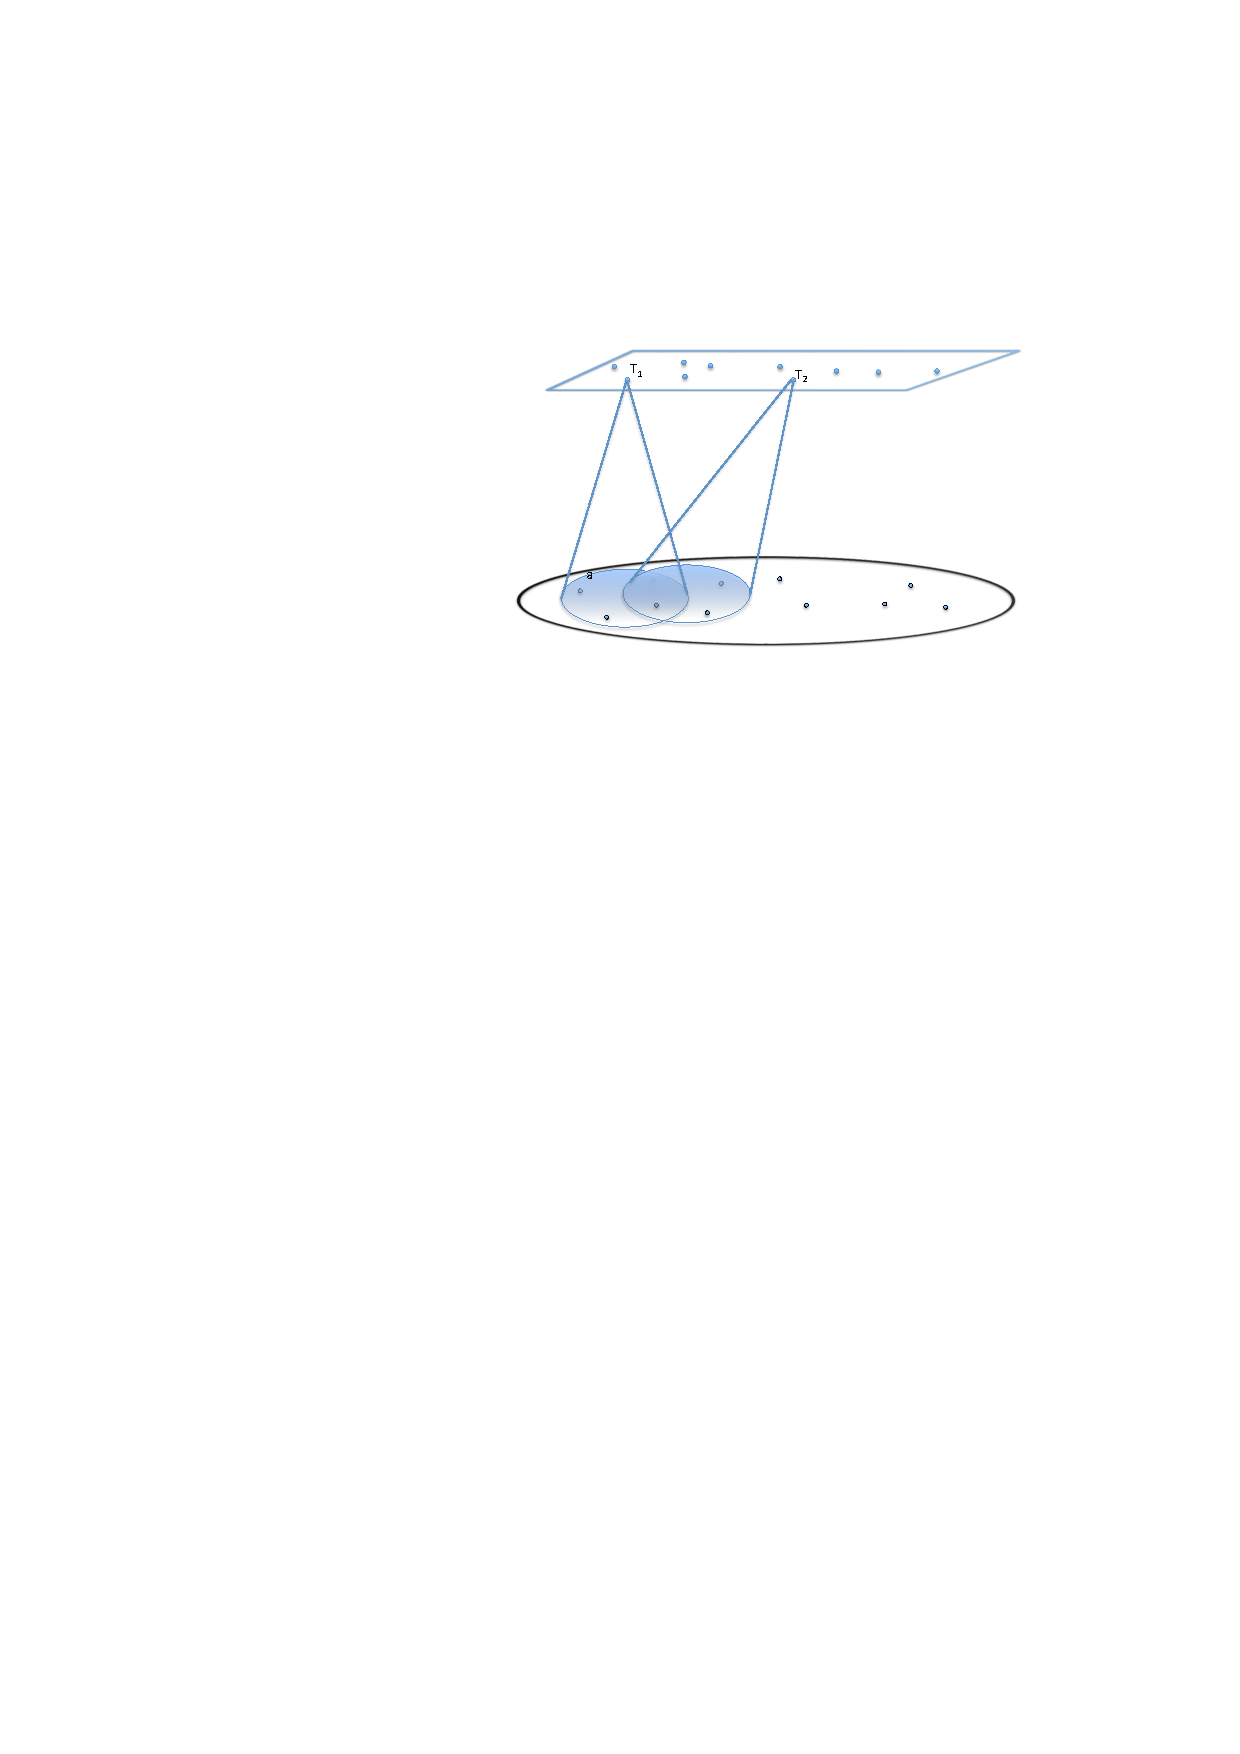
\includegraphics[width=\textwidth]{basic}
\begin{adjustbox}{max width=\textwidth}
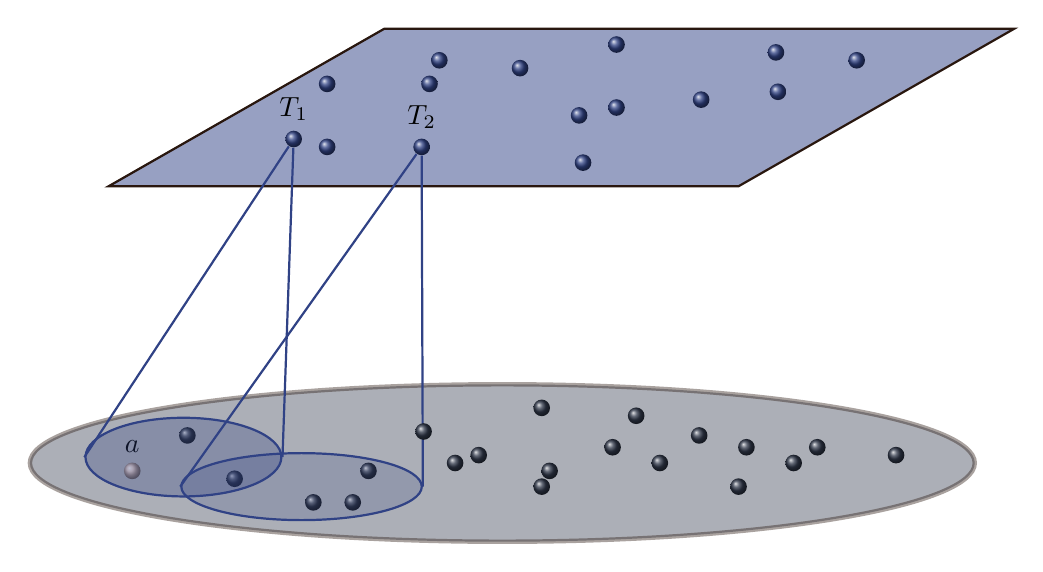
\begin{tikzpicture}[
  type/.style={circle, inner sep=0pt, minimum size=6pt, ball color=BTypeCol},
  firsttype/.style={circle, inner sep=0pt, minimum size=6pt, ball color=FirstTypeCol},
  secondtype/.style={circle, inner sep=0pt, minimum size=6pt, ball color=SecondTypeCol},
  objects/.style={circle, inner sep=0pt, minimum size=6pt, ball color=ObjectCol},
  modalobjects/.style={circle, inner sep=0pt, minimum size=6pt, ball color=ModalCol}
  ]

  % basic types:
  \begin{scope}[
    % every node/.append style={yslant=0,xslant=1.75},
    yslant=0,xslant=1.75
    ]
    \filldraw [fill=BTypeCol, draw=BorderCol, thick, fill opacity=0.5] (0,0) rectangle (8,2);

    \foreach \x/\y in {0.5/1.3, 1.4/1.6, 1.8/1.3, 1.9/0.5, 3.3/1.8, 2.6/1.5, 4.4/0.9, 4.7/1, 5.5/0.3, 5.6/1.1, 5.5/1.7, 6.4/1.2, 6.7/1.6} {
      \node [type] at (\x,\y) {};
    }

    \node [coordinate] (btypeleft) at (0,1) {};
    \node [coordinate] (btyperight) at (8,1) {};

    \node [type, label=above:$T_1$] (t1) at (1.3,0.6) {};
    \node [type, label=above:$T_2$] (t2) at (3.1,0.5) {};
  \end{scope}    


  % objects:
  \begin{scope}[
    % every node/.append style={yslant=0,xslant=1.75},
    %yslant=0,xslant=1.75,
    yshift=-100
    ]
    \filldraw [fill=ObjectCol, opacity=0.4, draw=BorderCol, ultra thick] (5,0) ellipse (6 and 1);

    \foreach \a/\b in {5.5/0.7, 6.4/0.2, 6.7/0.6, 7/0, 7.5/0.35, 8/-0.3, 8.1/0.2, 8.7/0, 9/0.2, 10/0.1} {
      \node [objects] at (\a,\b) {};
    }
    % for T1 from BType:
    \node [modalobjects, label=above:$a$] (o1) at (0.3,-0.1) {}; 
    \node [objects] (o2) at (1,0.35) {}; 
    \node [objects] (o3) at (1.6,-0.2) {};
    \node [ellipse, fit=(o1) (o2) (o3), yscale=0.7, draw=BTypeCol, thick, fill=BTypeCol, fill opacity=0.3] (fitA) {};
    \draw [BTypeCol, thick] (t1) -- (fitA.east);
    \draw [BTypeCol, thick] (t1) -- (fitA.west);

    % for T2 from BType:
    \node [objects] (o4) at (2.6,-0.5) {};
    \node [objects] (o5) at (3.1,-0.5) {};
    \node [objects] (o6) at (3.3,-0.1) {};
    \node [ellipse, fit=(o3) (o4) (o5) (o6), yscale=0.7, draw=BTypeCol, thick, fill=BTypeCol, fill opacity=0.2] (fitB) {};
    \draw [BTypeCol, thick] (t2) -- (fitB.east);
    \draw [BTypeCol, thick] (t2) -- (fitB.west);

    % % for T2 from Type1:
     \node [objects] (o7) at (4,0.4) {};
     \node [objects] (o8) at (4.4,0) {}; 
     \node [objects] (o9) at (4.7,0.1) {};
    % \node [ellipse, fit=(o3) (o4) (o5) (o6) (o7) (o8) (o9), yscale=0.6, xscale=0.9, draw=FirstTypeCol, thick, fill=FirstTypeCol, fill opacity=0.2] (fitC) {};

    % % for T2 from Type2:
     \node [objects] (o10) at (5.5,-0.3) {};
     \node [objects] (o11) at (5.6,-0.1) {};
    % \node [ellipse, fit=(o3) (o4) (o5) (o6) (o7) (o8) (o9) (o10) (o11), yscale=0.7, xscale=0.8, draw=SecondTypeCol, thick, fill=SecondTypeCol, fill opacity=0.2] (fitD) {};
  \end{scope}


  % % modal types:
  % \begin{scope}[
  %   % every node/.append style={yslant=0,xslant=1.75},
  %   %yslant=0,xslant=1.75,
  %   yshift=-35, 
  %   xshift=220
  %   ]
  %   \filldraw [fill=ObjectCol, opacity=0.4, draw=BorderCol, ultra thick] (3.5,0) ellipse (4 and 0.75);

  %   \foreach \a/\b in {0.3/-0.1, 1.5/-0.3, 3.9/0.2, 7/0} {
  %     \node [objects] at (\a,\b) {};
  %   }
  %   \node [modalobjects, label=above:$a$] at (0.7,0) {};
  %   \node [objects] (i1) at (5.7,-0.2) {};
  %   \node [objects] (i2) at (6.1,0.3) {};
  %   \node [objects] (i3) at (5,0) {};
  %   \node [ellipse, fit=(i1) (i2) (i3), yscale=0.7, draw=BTypeCol, thick, fill=BTypeCol, fill opacity=0.2] {};

  %   \node [objects] (i4) at (1.6,0.1) {};
  %   \node [objects] (i5) at (2,0.2) {};
  %   \node [modalobjects, label=above:$b$] (i6) at (2.5,-0.3) {};
  %   \node [objects] (i7) at (2.7,0.35) {};
  %   \node [ellipse, fit=(i4) (i5) (i6) (i7), yscale=0.7, xscale=1.1, draw=BTypeCol, thick, fill=BTypeCol, fill opacity=0.2] {};
  % \end{scope}


  % % Type1:
  % \begin{scope}[
  %   % every node/.append style={yslant=0,xslant=1.75},
  %   yslant=0,xslant=1.75,
  %   xshift=-100,
  %   yshift=80
  %   ]
  %   \filldraw [fill=FirstTypeCol, draw=BorderCol, thick, fill opacity=0.3] (0,0) rectangle (8,2);
  %   \node [coordinate] (firsttypeleft) at (0,1) {};
  %   \node [coordinate] (firsttyperight) at (8,1) {};

  %   \foreach \x/\y in {0.45/1.4, 1.4/1.6, 1.9/0.5, 3.3/1.8, 2.6/1.5, 4.7/1, 5.5/0.3, 5.6/1.1,  6.7/1.6} {
  %     \node [firsttype] at (\x,\y) {};
  %   }

  %   \node [firsttype, label=above:$T_1$] (ft1) at (1.8,1.1) {};
  %   \node [firsttype, label=above:$T_2$] (ft2) at (5.8,0.7) {};
  %   \node [firsttype, label=above:$T_3$] (ft3) at (6.4,1.2) {};
  %   \node [firsttype, label=above:{\textbf{Type$^1$}}] (ft) at (4,0.4) {};

  %   \draw [FirstTypeCol, thick] (ft) -- (btypeleft);
  %   \draw [FirstTypeCol, thick] (ft) -- (btyperight);
    
  %   \draw [FirstTypeCol, thick] (ft2) -- (fitC.east);
  %   \draw [FirstTypeCol, thick] (ft2) -- (fitC.west);
  % \end{scope}    


  % % Type2:
  % \begin{scope}[
  %   % every node/.append style={yslant=0,xslant=1.75},
  %   yslant=0,xslant=1.75,
  %   xshift=-200,
  %   yshift=160
  %   ]
  %   \filldraw [fill=SecondTypeCol, draw=BorderCol, thick, fill opacity=0.1] (0,0) rectangle (8,2);
  %   \foreach \x/\y in {1.4/1.6, 1.9/0.5, 3.2/1.5, 4.7/1, 5.4/1.2, 5.8/0.3, 6/0.3,  6.2/1.6} {
  %     \node [secondtype] at (\x,\y) {};
  %   }

  %   \node [secondtype, label=above:$T_1$] (st1) at (1.2,1) {};
  %   \node [secondtype, label=above:$T_2$] (st2) at (4.8,0.7) {};
  %   \node [secondtype, label=above:$T_3$] (st3) at (2.6,1.3) {};
  %   \node [secondtype, label=above:{\textbf{Type$^2$}}] (st) at (3.4,0.5) {};

  %   \draw [SecondTypeCol, thick] (st) -- (firsttypeleft);
  %   \draw [SecondTypeCol, thick] (st) -- (firsttyperight);
    
  %   \draw [SecondTypeCol, thick] (st2) -- (fitD.east);
  %   \draw [SecondTypeCol, thick] (st2) -- (fitD.west);
  % \end{scope}    
\end{tikzpicture}
\end{adjustbox}

\caption{System of basic types}
\label{fig:basic}
\end{figure}

A system of basic types consists of a set of types which are \textit{basic} in
the sense that they are not analyzed as
\textit{complex} entities composed of other entities in the theory.
Each of these types is associated with a set of objects, that is, the
objects which are of the type, the \textit{witnesses} for the type.  Thus if $T$ is a type and $A(T)$ is the
set of witnesses for $T$, then $a$ is of type $T$ (in
symbols, $a:T$) just in case $a\in A(T)$.  We require that any object $a$
which is a witness for a basic type is not itself one of the types in
the system.  A type may be \textit{empty} in the sense that it is
associated with the empty set, that is, there is nothing of that
type. 

Notice that we are starting with the types and associating sets
of objects with them.  This means that while there can be types for
which there are no witnesses, there cannot be objects which do not
belong to a type.  This relates back to our claim in
Section~\ref{sec:perc} that we cannot perceive an object without
assigning a type to it.

Notice also that the sets of objects associated with types may have
members in common.  Thus it is possible for objects to belong to more
than one type.  This is important if we want to have basic types
\textit{Elm}, \textit{Tree} and \textit{Physical Object} and say that
a single object $a$ belongs to all three types as discussed in
Section~\ref{sec:perc}.

An extremely important property of this kind of type system is that
there is nothing which prevents two types from being associated with
exactly the same set of objects.  In standard set theory the notion of
set is \textit{extensional}, that is sets are defined by their
membership.  You cannot have two distinct sets with the same members.
The choice of defining types as entities in their own right rather
than as the sets of their witnesses, means that they can be
\textit{intensional}, that is, you can have more than one type with
the same set of witnesses.  This can be important for the analysis of
natural language words like \textit{groundhog} and \textit{woodchuck}
which (as I have learned from the literature on natural language
semantics) are the same animal. In this case one may wish to say that
you have two different words which correspond to the same type, rather
than two types with the same \textit{extension} (that is, set of
witnesses).  Such an analysis is less appealing in the case of
\textit{unicorn} and \textit{centaur}, both mythical animals
corresponding to types which have an empty extension.  If types were
extensional, there would only be one empty type (just as there is only
one empty set in set theory).  In the kind of possible world semantics
espoused by Montague the distinction between \textit{unicorn} and
\textit{centaur} was made by considering their extension not only in
the actual world (where both are empty) but also in all possible
worlds, since there will be some worlds in which the extensions are
not the same.
However, this kind of possible worlds analysis of intensionality fails
when you have types whose extensions cannot possibly be different.
Consider \textit{round square} and \textit{positive number equal to
  $2-5$}.  The possible worlds analysis cannot distinguish between
these since their extensions are both empty no matter which possible
world you look at.

Finally, notice that there may be different systems of basic types,
possibly with different types and different objects.  One way of
exploiting this would be to associate different systems with different
organisms as discussed in Section~\ref{sec:perc}.  (Below we will see
different uses of this for the analysis of types which model the
cognitive system of a single
agent.) Thus properly we should say that an object $a$ is of type $T$
with respect to a basic systems of types {\bf TYPE$_B$}, in symbols,
$a:_{\mathbf{TYPE_B}}T$.  However,  we will continue
to write $a:T$ in our informal discussion when there is no danger of
confusion. 

The definition of a system of basic types is made precise in
\nexteg{}, which is repeated in
Appendix~\ref{sec:basic}.  

\begin{ex}
A {\it system of basic types\/} is a pair:
\begin{quote}
{\bf TYPE$_B$} = $\langle${\bf Type}, $A$$\rangle$
\end{quote}
where:
\begin{enumerate} 
 
\item \textbf{Type} is a non-empty set 
 
\item $A$ is a function whose domain is \textbf{Type}

\item for any $T\in\textbf{Type}$, $A(T)$ is a set disjoint from
  \textbf{Type}

\item for any $T\in\textbf{Type}$, $a:_{\mathbf{TYPE_B}}T$ iff $a\in A(T)$
 
\end{enumerate}

\label{ex:def-basic-types}
\end{ex} 

Some readers may prefer a slightly less formal characterization which
uses the kind of format normally employed in proof theory.  This may
provide a more easily readable overview of the definitions while
suppressing some of the details which are not necessary for intuitive
understanding.  We will use $\Gamma$, normally used for contexts in
prove theory, that is sequences of judgements to refer to type systems
like those characterized in \preveg{}.  Thus in \nexteg{} $\Gamma$
corresponds to \textbf{TYPE}$_B$.  We will write
$\Gamma\vdash T\in\textbf{Type}$ ``$T\in\textbf{Type}$ follows from
$\Gamma$'' to represent that \textbf{Type} is the set of types in
$\Gamma$  as
specified in \preveg{} and that the type $T$ is a member of this set.
We will similarly write $\Gamma\vdash a\in A(T)$ to indicate that
object $a$ is in the set assigned to $T$ by the function $A$ given by $\Gamma$.
We can then write a rule as in \nexteg{}.
\begin{ex} 
For $\Gamma$ a system of basic types:

\begin{prooftree}
\hypo{\Gamma\vdash T\in \textbf{Type}} \hypo{\Gamma\vdash a\in A(T)}
\infer2{\Gamma\vdash a:T}
\end{prooftree} 
\end{ex} 
We take this to be an inductive definition of the set of consequences.
That is, we are characterizing the smallest set of judgements
$\Gamma\vdash a:T$ which obey the premises.  In this way the inference
rule \preveg{} has the force of a biconditional corresponding to
clause~4 in (\ref{ex:def-basic-types}).   

What counts as an object may vary from agent to agent
(particularly if agents are of different species).  Different agents
have what \cite{Barwise1989} would call different \textit{schemes
  of individuation}.  There appears to be a complex relationship
between the types that an agent is attuned to and the parts of the
world which the agent will perceive as an object.  We model this in
part by allowing different type systems to have different
objects.  In addition we will make extensive use in our systems of a
basic type \textit{Ind} for ``individual'' which corresponds to
Montague's notion of ``entity''.  The type \textit{Ind} might be
thought of as modelling a large part of an agent's scheme of
individuation in Barwise's sense.  However, this clearly still leaves
a great deal to be explained and we do this in the hope that exploring the nature of the type
systems involved will ultimately give us more insight into how
individuation is achieved.


\section{Situation types}
\label{sec:sittypes}

Kim continues her walk in the park.  She sees a boy playing with a dog
and notices that the boy gives the dog a hug.  In perceiving this
event she is aware that two individuals are involved and that there is
a relation holding between them, namely hugging.  She also perceives
that the boy is hugging the dog and not the other way around.  She
sees that a certain action (hugging) is being performed by an agent
(the boy) on a patient (the dog).  This perception seems more complex
than the classification of an individual object as a tree in the sense
that it involves two individual participants and a relation between
them as well as the roles those two individuals play in the relation.
While it is undoubtably more complex than the simple classification of
an object as a tree, we want to say that it is still the assignment of
a type to an object.  The object is now an event and she classifies
the event as a hugging event with the boy as agent and the dog as
patient.  We shall have complex types which can be assigned to such events.

\textit{Complex} types are constructed out of
other entities in the theory.  As we have just seen,
cognitive agents, in addition to being able to assign types to
individual objects like trees, also perceive the world in terms of states and
events where objects have properties and stand in relations to each
other -- what \cite{Davidson1967} called events and
\cite{BarwisePerry1983} called situations.  

\subsection{Types constructed from predicates (ptypes)}
\label{sec:ptypes}
We
introduce types which are constructed from predicates (like `hug') and
objects which are arguments to this predicate like $a$ and $b$.  We
will represent such a constructed type as hug($a$,$b$) and we will
call it a \textit{ptype} to indicate that it is a type whose
main constructor is a predicate.  What would an
object belonging to such a type be?  According to the type-theoretic
approach introduced by Martin-L�f it should be an object which
constitutes a proof that $a$ is hugging $b$.  For Martin-L�f, who was
considering mathematical predicates, such proof objects might be numbers
with certain properties, ordered pairs and so on.  \cite{Ranta1994}
points out that for non-mathematical predicates the objects could be
events as conceived by \cite{Davidson1967,Davidson1980}.  Thus hug($a$,$b$) can be
considered to be an event or a situation type.  In some versions of
situation theory \cite{Barwise1989,SeligmanMoss1997}, objects (called \textit{infons})
constructed from a relation and its arguments was considered to be one
kind of situation type.  Thus one view would be that 
ptypes are playing a similar role in type theory to the role that
infons play in situation theory.

What kind of entity are predicates?  \ignore{The notion is made precise in
Appendix~\ref{app:predicates}.}  One important fact about predicates
is that they come along with an \textit{arity}.  The arity of a
predicate tells you what kind of arguments the predicate takes and
what order they come in. For us the arity of a predicate will be a
sequence of types.  The predicate `hug' as discussed above we can
think of as a two-place predicate both of whose arguments must be of
type \textit{Ind}, that is, an individual.  Thus the arity of `hug'
will be $\langle$\textit{Ind}, \textit{Ind}$\rangle$.  The idea is
that if you combine a predicate with arguments of the appropriate
types in the appropriate order indicated by the arity then you will
have a type.  Thus if $a$ : \textit{Ind} and $b$ : \textit{Ind} then
hug($a$,$b$) will be a type, intuitively the type of situation where
$a$ hugs $b$.  

We will introduce a function \textit{Arity} which is
defined on predicates and which assigns an arity to any predicate.
This function is introduced in a \textit{predicate signature} which in
addition tells you what predicates there are and what we can use to
characterize their arguments (a set of types in the way we will use
this. We define a predicate signature by the definition in \nexteg{}
(repeated in Appendix~\ref{app:predicates}).
\begin{ex} 
A \textit{predicate signature} 
is a triple
\begin{quote}
$\langle$\textbf{Pred}, \textbf{ArgIndices}, \textit{Arity}$\rangle$
\end{quote}
where:
\begin{enumerate} 
 
\item \textbf{Pred} is a set (of predicates)

\item \textbf{ArgIndices} is a set (of indices for predicate
  arguments, normally types)
 
\item \textit{Arity} is a function with domain \textbf{Pred} and range
  included in the set of finite sequences of members of \textbf{ArgIndices}. 
 
\end{enumerate}
\label{ex:pred-sig} 
\end{ex}
A simple example of a predicate signature would be given by \nexteg{}.
\begin{ex} 
\begin{subex} 
 
\item \textbf{Pred} = \{boy, dog, hug\} 
 
\item \textbf{ArgIndices} = \{\textit{Ind}\}

\item \textit{Arity} is defined by:
\begin{quote}
\textit{Arity}(boy) = $\langle\textit{Ind}\rangle$\\
\textit{Arity}(dog) = $\langle\textit{Ind}\rangle$\\
\textit{Arity}(hug) = $\langle\textit{Ind}, \textit{Ind}\rangle$
\end{quote} 
 
\end{subex} 
   
\end{ex} 
   
  

It may be desirable to allow some predicates to combine with more than
one assortment of argument types.  Thus, for example, one might wish
to say that the predicate `believe' can combine with two individuals
just like `hug' (as in \textit{Kim believes Sam}) or with an
individual and a ``proposition'' (as in \textit{Kim believes that Sam
  is telling the truth}).  Similarly the predicate `want' might be
both a two-place predicate for individuals (as in \textit{Kim wants
  the tree}) or a two-place predicate between individuals and
``properties'' (as in \textit{Kim wants to own the tree}).  We shall
have more to say about ``propositions'' and ``properties'' later.  For
now, we just note that we want to allow for the possibilities that
predicates can be \textit{polymorphic} in the sense that there may be
more than one sequence of types which characterize the arguments they
are allowed to combine with.  The sequences need not even be of the
same length (consider \textit{Kim walked} and \textit{Kim walked the
  dog}).  We thus allow for the possibility that these pairs of natural
language examples can be treated using the same polymorphic
predicate.  Another possibility, of course, is to say that the English
verbs can correspond to different (though related) predicates in the
example pairs and not allow this kind of predicate polymorphism in the
type theory. We do not take a stand on this issue but merely note that
both possibilities are available.  If predicates are to be considered
polymorphic then the arity of a predicate can be considered to be a
set of sequences of types.  In \nexteg{} we give a definition of
a polymorphic predicate signature (repeated in Appendix~\ref{app:predicates}).
\begin{ex} 
A \textit{polymorphic predicate signature} 
is a triple 
\begin{quote}
$\langle$\textbf{Pred}, \textbf{ArgIndices}, \textit{Arity}$\rangle$
\end{quote}
where:
\begin{enumerate} 
 
\item \textbf{Pred} is a set (of predicates)

\item \textbf{ArgIndices} is a set (of indices for predicate
  arguments, normally types)
 
\item \textit{Arity} is a function with domain \textbf{Pred} and range
  included in the powerset of the set of finite sequences of members
  of \textbf{ArgIndices}. 
 
\end{enumerate}
\label{ex:poly-pred-sig} 
\end{ex} 
A simple example of a polymorphic predicate signature is given in
\nexteg{}.
\begin{ex} 
\begin{subex} 
 
\item \textbf{Pred} = \{boy, dog, hug, walk\} 
 
\item \textbf{ArgIndices} = \{\textit{Ind}\}

\item \textit{Arity} is defined by:
\begin{quote}
\textit{Arity}(boy) = $\{\langle\textit{Ind}\rangle\}$\\
\textit{Arity}(dog) = $\{\langle\textit{Ind}\rangle\}$\\
\textit{Arity}(hug) = $\{\langle\textit{Ind}, \textit{Ind}\rangle\}$\\
\textit{Arity}(walk) = $\{\langle\textit{Ind}\rangle, \langle\textit{Ind}, \textit{Ind}\rangle\}$
\end{quote} 
 
\end{subex} 
   
\end{ex}   

An alternative to our characterization of predicates is to consider them as functions from sequences of objects
matching their arity to types.  As such they would be a
\textit{dependent type}, that is, an entity which returns a type when
provided with an appropriate object or sequence of objects.  However,
we have not done this because we want all those entities we call
dependent types to be representable as $\lambda$-expressions.  We can,
however, think of them as \textit{type constructors} as will be made
clear in our discussion of systems of complex types below.

A \textit{system of complex types} \ignore{(made precise in Appendix~\ref{app:comptypes})}
adds to a system of basic types a collection of types constructed from
a set of predicates with their arities, that is, it adds all the types
which you can construct from the predicates by combining them with
objects of the types corresponding to their arities according to the
types in the rest of the system.  The system also assigns a set of
objects to all the types thus constructed from predicates.  Many of
these types will be assigned the empty set.  Intuitively, if we have a
type hug($c$,$d$) and there are no situations in which $c$ hugs $d$
then there will be nothing in the extension of hug($c$,$d$), that is,
it will be assigned the empty set in the system of complex types.
Notice that the intensionality of our type system becomes very
important here.  There may be many individuals $x$ and $y$ for which
hug($x$,$y$) is empty but still we would want to say that the types
resulting from the combination of  `hug'
with the various different individuals corresponds to
different types of situations.  The formal characterization of a
system of complex types is given in \nexteg{} (repeated in
Appendix~\ref{app:comptypes}).
\begin{ex} 
A {\it system of complex types\/} is a quadruple:
\begin{quote}
{\bf TYPE$_C$} = $\langle${\bf Type}, {\bf BType},
$\langle$\textbf{PType}, {\bf Pred}, \textbf{ArgIndices}, {\it Arity\/}$\rangle$, $\langle A,F\rangle$$\rangle$
\end{quote}
where:  
\begin{enumerate} 
 
\item $\langle$\textbf{BType}, $A$$\rangle$ is a system of basic types 
 
\item \textbf{BType}$\subseteq$\textbf{Type}

\item for any $T\in\textbf{Type}$, if $a:_{\langle\mathbf{BType},
    A\rangle}T$ then $a:_{\mathbf{TYPE_C}}T$

\item \label{cl:predtypes}$\langle${\bf Pred}, \textbf{ArgIndices},
  {\it Arity\/}$\rangle$ is a (polymorphic) predicate
  signature

\item\hspace*{-1ex}\ignore{\footnote{This clause has been modified since
    \cite{Cooper2012} where it was a conditional rather than a biconditional.}} %\sloppy  
  $P(a_1,\ldots a_n)\in\textbf{PType}$ iff $P\in\textbf{Pred}$, $T_1\in \mathbf{Type},\ldots,T_n\in
  \mathbf{Type}$, \textit{Arity}($P$)=$\langle
  T_1,\ldots,T_n\rangle$  ($\langle
  T_1,\ldots,T_n\rangle$$\in$\textit{Arity}($P$)) and $a_1:_{\mathbf{TYPE_C}}T_1,\ldots,a_n:_{\mathbf{TYPE_C}}T_n$

% If $P\in\textbf{Pred}$, $T_1\in \mathbf{Type},\ldots,T_n\in
%   \mathbf{Type}$, \textit{Arity}($P$)=$\langle
%   T_1,\ldots,T_n\rangle$  ($\langle
%   T_1,\ldots,T_n\rangle$$\in$\textit{Arity}($P$)) and $a_1:_{\mathbf{TYPE_C}}T_1,\ldots,a_n:_{\mathbf{TYPE_C}}T_n$ then
%   $P(a_1,\ldots a_n)\in\textbf{PType}$



\item \textbf{PType}$\subseteq$\textbf{Type}

\item for any $T\in\textbf{PType}$, $F(T)$ is a set disjoint from \textbf{Type}

\item for any $T\in\textbf{PType}$, $a:_{\mathbf{TYPE_C}}T$ iff $a\in F(T)$
 
\end{enumerate} 
\label{ex:comp-types}
\end{ex} 
\preveg{} perhaps looks a little forbidding for something that says
that if you have a predicate $P$ whose arity is $\langle
T_1,\ldots,T_n\rangle$ and you have objects $a_1:T_1,\ldots,a_n:T_n$
then $P(a_1,\ldots,a_n)$ is a ptype and any ptype is also a type.  In
this definition we have not made explicit exactly what set theoretic
object we are representing with $P(a_1,\ldots,a_n)$.  We will take
this up below (in Section~\ref{sec:labelled-sets}) since it is part of
a general strategy we employ for representing objects in our type
theory as sets.  
\preveg{} also gives us a function $F$ which maps ptypes to a set of
witnesses and it also makes clear that a system of complex types adds
to a system of basic types.  The set of types of the new system
consists of the basic types and the ptypes.  Perhaps the informal
proof theoretic notation in \nexteg{} is a little less forbidding.
\begin{ex}
For $\Gamma$ a system of complex types: 
\begin{subex} 
 
\item  \begin{prooftree}
\hypo{\Gamma\vdash T\in\textbf{BType}} \hypo{\Gamma\vdash a\in A(T)}
\infer2{\Gamma\vdash a:T}
\end{prooftree}
 
\item \begin{prooftree}
\hypo{\Gamma\vdash T\in \textbf{BType}} \infer1{\Gamma\vdash
  T\in\textbf{Type}}
\end{prooftree}

\item \begin{prooftree}
\hypo{\Gamma\vdash P\in\textbf{Pred}} \hypo{\Gamma\vdash \langle
  T_1,\ldots,T_n\rangle=\textit{Arity}(P)} \hypo{\Gamma\vdash
  a_1:T_1,\ldots,\Gamma\vdash a_n:T_n} \infer3{\Gamma\vdash
  P(a_1,\ldots,a_n)\in\textbf{PType}}
\end{prooftree}

\medskip

or alternatively if we are considering our predicates to be
polymorphic:

\medskip

\begin{prooftree}
\hypo{\Gamma\vdash P\in\textbf{Pred}} \hypo{\Gamma\vdash \langle
  T_1,\ldots,T_n\rangle\in\textit{Arity}(P)} \hypo{\Gamma\vdash
  a_1:T_1,\ldots,\Gamma\vdash a_n:T_n} \infer3{\Gamma\vdash
  P(a_1,\ldots,a_n)\in\textbf{PType}}
\end{prooftree}

\item \begin{prooftree}
\hypo{\Gamma\vdash T\in\textbf{PType}} \infer1{\Gamma\vdash
  T\in\textbf{Type}}
\end{prooftree}

\item \begin{prooftree}
\hypo{\Gamma\vdash T\in\textbf{PType}} \hypo{\Gamma\vdash s\in F(T)}
\infer2{\Gamma\vdash s:T}
\end{prooftree} 
 
\end{subex} 
   
\end{ex} 
\preveg{a} is the rule that we had for basic type systems except that
we have identified the relevant set of types as \textbf{BType} (the
basic types).  \preveg{b} tells us that \textbf{BType} is a subset of
\textbf{Type}. \preveg{c} tells us how to form ptypes from a predicate
and an appropriate sequence of objects. \preveg{d} tells us that
ptypes are types.  \preveg{e} tells us that the witnesses of ptypes
are determined by the function $F$.
  

There are thus two important functions
in a system of complex types:  one, which we call $A$, which comes from
the system of basic types embedded in the system and assigns
extensions to basic types and the other, which we call $F$, which
assigns extensions to types constructed from predicates and arguments
corresponding to the arity of the predicates.  We have chosen the
letters $A$ and $F$ because they are used very often in the
characterization of models \label{pg:models} of first order logic.  A model for first
order logic is often characterized as a pair $\langle A,F\rangle$
where $A$ is the domain and $F$ a function which assigns denotations to
the basic expressions (constants and predicates) of the logic.  In a
slight variation on classical first order logic $A$ may be a sorted
domain, that is the domain is not a single set but a set divided into
various subsets, corresponding to \textit{sorts}. For
us, $A$ characterizes assignments to basic types and thus provides
something like a sorted domain in first order model theory.  In first
order logic $F$ gives us what we need to know to determine the truth
of expressions like `hug($a$,$b$)' in first order logic.  Thus $F$ will
assign to the predicate `hug' a set of ordered pairs telling us who
hugs whom.  Our $F$ also give us the information we need in order to
tell who stands in a predicate relation.  However, it does this, not
by assigning a set of ordered $n$-tuples to each predicate, but by
assigning sets of witnesses (or ``proofs'') to each type constructed from a predicate with
appropriate arguments.  The set of ordered pairs assigned to `hug' by
the first order logic $F$ corresponds to the set of pairs of arguments
$\langle x,y\rangle$ for which the $F$ in a complex system of types
assigns a non-empty set.  For this reason we call the pair $\langle
A,F\rangle$ a \textit{model} within the type system, even though it is not
technically a model in the sense of model theory for logic.  The
correspondence becomes important below, when we talk about modal type
systems.

What are the entities which are witnesses for ptypes?  The intuition is
that, for example, \nexteg{} means that $e$ is an event or situation where the individual $a$ is
running.
\begin{ex}
$e$ : run($a$)
\end{ex}
There are two competing intuitions about what $e$ could be.
One is that it is a ``part of the world'', a non-set (urelement).  That is, from
the perspective of set theory and the theory of types it is an unstructured
atom.  The other intuition we have is that it is a structured entity which
contains $a$ as a component and in which a running activity is going
on which involves smaller events such as picking feet up off the
ground, spending certain time in each step cycle with neither foot
touching the ground and so on.  We want to allow for both of these
intuitions.  That is, a witness for a ptype can be a non-set
corresponding to our notion of an event of a certain type.  Or it can
be the kind of labelled set which we call a record (see
Section~\ref{sec:rectypes}).  That is, $e$ is not only a witness for
the type `run($a$)' but also for a record type which
characterizes in more detail the structure of the event.  We will
argue that both intuitions are important and that
observers of the world shift between views where certain
ptypes are regarded as types of non-sets and views where those
ptypes are types of records.

The introduction of predicates  and ptypes raises
the question of how one-place predicates relate to basic types.  For
example, what is the relationship between a type \textit{Dog} whose
witnesses are dogs and a predicate `dog' whose arity is
$\langle\textit{Ind}\rangle$.  One way to relate the two is given in
\nexteg{}.
\begin{ex} 
$a:\textit{Dog}$ iff $\exists e\ e:\text{dog}(a)$ 
\end{ex} 
\preveg{} says that something is of type \textit{Dog} just in case
there is a situation which shows it to fall under the predicate
`dog'. In this book we will relate common nouns to predicates rather
than basic types, in part because common nouns can sometimes have
more than one argument and in part because we want to limit the number
of basic types we use.  If we need a type we can derive it from the
predicate using something like \preveg{}.

% We said above that the arity of `hug' is
% $\langle$\textit{Ind},\textit{Ind}$\rangle$.  However, when we look at
% (\ref{eg:rectype}b) where the types labelled with `x' and `y' are
% \textit{Boy} and \textit{Dog} we see that there is nothing explicit here that
% requires that the two arguments of `hug' are of type \textit{Ind}.
% One obvious way to achieve this would be to require that \textit{Boy}
% and \textit{Dog} are subtypes of \textit{Ind}, that is, that any
% object of type \textit{Boy} is also of type \textit{Ind} and similarly
% for \textit{Dog}.  However, now that we have introduced predicates
% there is nothing to stop us having two predicates `boy' and `dog' with
% arity $\langle$\textit{Ind}$\rangle$.  Thus we could have the record
% type \nexteg{}.
% \begin{ex} 
% \record{\tfield{x}{\textit{Ind}} \\
%         \tfield{c$_{\mathrm{boy}}$}{boy(x)} \\
%         \tfield{y}{\textit{Ind}} \\
%         \tfield{c$_{\mathrm{dog}}$}{dog(y)} \\
%               \tfield{c$_{\mathrm{hug}}$}{hug(x,y)}} 
% \end{ex} 
% How do we choose between a type like \preveg{} where common nouns like
% \textit{boy} and \textit{dog}
% correspond to one-place predicates and a type like
% (\ref{eg:rectype}{b}) where common nouns correspond to basic types?
% One advantage is that \preveg{} explicitly represents that the arity
% of `hug' is fulfilled.  Another advantage is that many, and on some
% analyses possibly all,
% nouns in natural languages will in more detailed treatments correspond
% to predicates of more than one argument.  Consider, for example, the
% fact that boys grow into men.  The same individual can be a boy at one
% time and a man at a later time.  One way of treating this is to say
% that  `boy' is a predicate of
% two arguments with arity
% $\langle$\textit{Ind},\textit{Time}$\rangle$.  In fact if we are going
% to deal with tense and aspect in natural language in this way we will probably
% want to add time arguments to most if not all of our predicates and
% thus allow ourselves record types like \nexteg{}.
% \begin{ex} 
% \record{\tfield{e-time}{\textit{Time}} \\
% \tfield{x}{\textit{Ind}} \\
%         \tfield{c$_{\mathrm{boy}}$}{boy(x,e-time)} \\
%         \tfield{y}{\textit{Ind}} \\
%         \tfield{c$_{\mathrm{dog}}$}{dog(y,e-time)} \\
%               \tfield{c$_{\mathrm{hug}}$}{hug(x,y,e-time)}} 
% \end{ex} 
% where `e-time' stands for ``event time''.  Here we have required that
% the times in all the predicate fields be the event time but this is
% not always the case.  Consider \nexteg{}.
% \begin{ex} 
% The minister smoked pot in his youth 
% \end{ex} 
% Here the time of the pot-smoking event most likely precedes 
% the time of the pot-smoking individual being a minister. We will thus
% use our basic types for basic ontological categories like \textit{individual}
% and \textit{time} and use predicates for words that occur in natural
% language.  Predicates can be $n$-ary whereas our types will always be
% unary.  Note that a ptype like hug($a$,$b$,$t$) is constructed from a
% ternary predicate `hug' but the type itself is a unary type of
% situations.  Thus we might have the judgement $s$ : hug($a$,$b$,$t$).

% Below we will propose an alternative to this treatment of
% time as an argument.  There is, however, another reason for allowing predicates
% corresponding to nouns to have more than one argument.  This is the existence of relational nouns such as \textit{friend}
% or \textit{daughter}.  (See \citealp{ParteeBorschev2012} for recent
% discussion.)

% In this book we will reserve basic types for two kinds of types:  (i)
% those which correspond to intuitively fundamental ontological categories
% such as individual and (ii) those types which require a recursive
% definition to characterize the set of their witnesses.  The latter is
% for a technical reason:  defining recursive types as, for instance,
% record types could lead to the types themselves being a
% non-well-founded set of ordered pairs which contain themselves.  We
% will discuss this more (????) when recursive types become relevant.


\subsection{Representing complex entities as labelled sets}
\label{sec:labelled-sets}
When we characterized ptypes in Section~\ref{sec:ptypes}, we did not
make explicit exactly which set-theoretic entity we were representing
by the notation for a ptype `$P(a_1,\ldots,a_n)$'.  In general complex
entities in our theory will be a particular kind of set.

We introduce a notion \textit{labelled sets} to model our complex entities. We
will assume that our set theory comes equipped with a set of
\textit{urelements} (entities which are not sets but which can be
members of sets).  We will assume that among the urelements is a countably infinite
set which is designated as the set of labels.  A \textit{labelled set}
(see also Appendix~\ref{app:sets}) is a set
of ordered pairs whose first member is a label and whose second
element is either an urelement which is not a label or a set (possibly a labelled
set), such that no more than one ordered pair can contain any
particular label as its first member.  This means that a labelled set
is the traditional set theoretic construction of an extensional
function from a set of labels onto some set.  Suppose that we have a
set \nexteg{a}
and that $\ell_0,\ell_1,\ell_2,\ell_3$ are labels.  Then examples of
labelled sets which are \textit{labellings} of \nexteg{a} would be \nexteg{b
  and c}.
\begin{ex} 
\begin{subex} 
 
\item $\{a,b,c,d\}$ 
 
\item
  $\{\langle\ell_0,a\rangle,\langle\ell_1,b\rangle,\langle\ell_2,c\rangle,\langle\ell_3,d\rangle\}$

\item $\{\langle\ell_0,\{\langle\ell_0,a\rangle,\langle\ell_1,b\rangle\}\rangle,\langle\ell_2,c\rangle,\langle\ell_3,d\rangle\}$ 
 
\end{subex} 
\label{ex:labelled-sets}   
\end{ex} 
We will refer to the first members of the pairs which constitute a
labelled set as \textit{labels} use in the labelled set and we will refer to
the second members of the ordered pairs as the \textit{labelled
  elements} of the labelled set.  If $X$ is a labelled set, we will
use $\mathrm{labels}(X)$ to represent the set of labels of $X$, that is,
the left projection of $X$ which means the set of objects which are
first members of the set of ordered pairs which are members of $X$.
Note that this means that if $X$ is the labelled set \preveg{c}, then
$\mathrm{labels}(X)$ is $\{\ell_0,\ell_2,\ell_3\}$, that is, the set of
those labels which occur at the topmost level of $X$, not including the set of
labels that occur within a labelled set contained in $X$, which in
this case would in addition include the label $\ell_1$.  If $X$ is a
labelled set and $\ell\in\mathrm{labels}(X)$ we will use $X.\ell$ to
represent the entity labelled by $\ell$.  Thus if $X$ is \preveg{b},
$X.\ell_0$ is $a$.  We can also define the set of \textit{paths} in
labelled sets given by the definition in \nexteg{}.
\begin{ex} 
If $X$ is a labelled set, then
\begin{enumerate} 
 
\item if $\ell\in\mathrm{labels}(X)$, then $\ell\in\mathrm{paths}(X)$ 
 
\item if $\ell\in\mathrm{labels}(X)$, $X.\ell$ is a labelled set and
  $\pi\in\mathrm{paths}(X.\ell)$, then $\ell.\pi\in\mathrm{paths}(X)$
\end{enumerate}  
\end{ex} 
By this definition the set of paths in (\ref{ex:labelled-sets}c) is
\nexteg{}.
\begin{ex} 
$\{\ell_0,\ell_2,\ell_3,\ell_0.\ell_0,\ell_0.\ell_1\}$ 
\end{ex} 
Note also that by these definitions, if $X$ is
(\ref{ex:labelled-sets}c), then $X.\ell_0.\ell_0$ is $a$, that is, we
can use the dot notation to take us down to a value on any path in the
labelled set.   

There are various ways in which labelled sets could be represented
graphically.  One way to represent the examples in (\ref{ex:labelled-sets}b and c)
would be as in \nexteg{}.
\begin{ex} 
\begin{subex} 
 
\item \mbox{\Tree [.$\ell_0$ \{$a$, ]\hspace*{1em} \Tree [.$\ell_1$ $b,$ ]\hspace*{1em} \Tree
  [.$\ell_2$ $c,$ ]\hspace*{1em} \Tree [.$\ell_3$ $d$\} ]}
 
\item \mbox{\Tree [.$\ell_0$ [.$\ell_0$ \{$a$, ] [.$\ell_1$ $b$, ] ]}  \raisebox{-2.054em}{\hspace*{1em}\Tree
  [.$\ell_2$ $c,$ ]\hspace*{1em} \Tree [.$\ell_3$ $d$\} ]}


 
\end{subex} 
   
\end{ex} 
  
  
Labelled sets where we identify particular distinguished labels will
always give us enough structure to model the structured entities that
we need and define operations on them as required by our theory of types.

The entity 
represented by $P(a_1,\ldots a_n)$ is the
labelled set in \nexteg{} where `pred', `arg$_i$' are reserved labels
(that is, not used except as
required here).
\begin{ex}
$\{\langle\mathrm{pred},P\rangle,\langle\mathrm{arg}_1,a_1\rangle,\ldots,\langle\mathrm{arg}_n,a_n\rangle\}$
\end{ex}



\subsection{Record types}
\label{sec:rectypes}
Kim sees a situation where $a$ (the boy) hugs $b$ (the dog) and
perceives it to be of type `hug($a$,$b$)'.  However, there are
intuitively other types which she could assign to this situation other
than the type of situation where $a$ hugs $b$ which is represented
here.  For example, a more general type, which would be useful in
characterizing all situations where hugging is going on between any
individuals, is that of ``situation where one
individual hugs another individual''.  Another type of situation she
might use is that of ``situation where a boy hugs a dog''.  This is a
more specific type than ``situation where one
individual hugs another individual'' but still does not tie us down to
the specific individuals $a$ and $b$ as the type `hug($a$,$b$)' does.

There are at least two different ways in type theory to approach
these more general types.  One is to use \textit{$\Sigma$-types} \label{pg:sigmatypes} such
as \nexteg{}.
\begin{ex} 
\begin{subex} 
 
\item $\Sigma x$:\textit{Ind}.$\Sigma y$:\textit{Ind}.hug($x$,$y$)
 
\item $\Sigma x$:\textit{Boy}.$\Sigma y$:\textit{Dog}.hug($x$,$y$) 
 
\end{subex} 
   
\end{ex}
% \preveg{b} uses the types \textit{Boy} and \textit{Dog} but we could
% also use ptypes constructed from the predicates `boy' and `dog' as
% discussed in Section~\ref{sec:ptypes} as in \nexteg{}.
% \begin{ex} 
% $\Sigma x$:\textit{Ind}.$\Sigma s_1$:boy($x$).$\Sigma
% y$:\textit{Ind}.$\Sigma s_2$:dog($y$).hug($x$,$y$) 
% \end{ex} 
  
We will use the notation $T\dep{x_1,\ldots,x_n}$ to represent that the
type $T$ depends on $x_1,\ldots,x_n$.  For example, the types
`hug($x$,$y$)' represented within the expressions in \preveg{} depend
on $x$ and $y$.
In general $\Sigma
x$:$T_1.T_2\dep{x}$ will have as witnesses any ordered pair the first
member of which is a witness for $T_1$ and the second member of which
is a witness for $T_2\dep{x}$.  Thus this type will be non-empty
(``true'') just in case there is something $a$ of type $T_1$ such that
there is something of type $T_2\dep{a}$.  This means that $\Sigma$-types
correspond to existential quantification.  A witness for \preveg{a} would be $\langle a,
\langle b, s\rangle\rangle$ where $a$:\textit{Ind}, $b$:\textit{Ind}
and $s$:hug($a$,$b$).  If there is such a witness then some individual
hugs another individual and conversely if some individual hugs another
individual there will be a witness for this type.  $\Sigma$-types are
exploited for the semantics of natural language by \cite{Ranta1994}
among others.

Another approach to these more general types is to use \textit{record
  types} such as \nexteg{a,b} or, as we will prefer given our decision
in Section~\ref{sec:ptypes}
to use ptypes constructed from predicates rather than types
corresponding to common nouns, \nexteg{c}.
\begin{ex}
\begin{subex} 
 
\item \record{\tfield{x}{\textit{Ind}} \\
              \tfield{y}{\textit{Ind}} \\
              \tfield{e}{hug(x,y)}}
 
\item \record{\tfield{x}{\textit{Boy}} \\
              \tfield{y}{\textit{Dog}} \\
              \tfield{e}{hug(x,y)}} 

\item \record{\tfield{x}{\textit{Ind}} \\
              \tfield{c$_1$}{boy(x)} \\
              \tfield{y}{\textit{Ind}} \\
              \tfield{c$_2$}{dog(y)} \\
              \tfield{e}{hug(x,y)}}
 
\end{subex} 
\label{ex:rectype} 
\end{ex} 
\ignore{We make the notion of record type precise in
Appendix~\ref{app:rectypes}.}  In TTR, record types are labelled
sets.  A first approximation to the labelled sets represented in
\preveg{} is given in \nexteg{}.  (In Section~\ref{sec:depfields} we will introduce
a complication in connection with the dependency represented by
`hug(x,y)', `boy(x)' and `dog(y)'.)
\begin{ex} 
\begin{subex} 
 
\item \{$\langle$x, \textit{Ind}$\rangle$, $\langle$y,
  \textit{Ind}$\rangle$, $\langle$e, hug(x, y)$\rangle$\} 
 
\item \{$\langle$x, \textit{Boy}$\rangle$, $\langle$y,
  \textit{Dog}$\rangle$, $\langle$e, hug(x, y)$\rangle$\} 

\item \{$\langle$x, \textit{Ind}$\rangle$, $\langle$c$_1$,
  boy(x)$\rangle$, $\langle$y,
  \textit{Ind}$\rangle$, $\langle$c$_2$, dog(y)$\rangle$, $\langle$e, hug(x, y)$\rangle$\} 
 
\end{subex} 
   
\end{ex} 
`x', `y', `c$_1$', `c$_2$' and `e' are particular labels.  In record types, the ordered
pairs whose first member is a label are called \textit{fields}.  Thus
record types are sets of fields.  We will give a precise
characterization of which labelled sets are record types later. 

The witnesses of record types are \textit{records}.  These
are also labelled sets, consisting of ordered pairs which we will call
fields of the record.  However, in this case the fields consist of a
label and an object belonging to a type, rather than a type, as in the
fields of record types.  A record, $r$, is a witness for a record
type, $T$, just in case $r$ contains fields with the same labels as
those in $T$  and the objects in the fields in $r$ are of the type
with the corresponding label in $T$.  The record may contain
additional fields with labels not mentioned in the record type with
the restriction there can only be one field within the record with a
particular label.  Thus both \nexteg{a} and \nexteg{b} are records of
type (\ref{ex:rectype}a).
\begin{ex} 
\begin{subex} 
 
\item \begin{tabular}{lp{.6\textwidth}}\record{\field{x}{$a$} \\
              \field{y}{$b$} \\
              \field{e}{$s$} } &  where $a$:\textit{Ind},
            $b$:\textit{Ind} and $s$:hug($a$,$b$) \end{tabular}
 
\item \begin{tabular}{lp{.6\textwidth}}\record{\field{x}{$c$} \\
              \field{y}{$d$} \\
              \field{e}{$s'$} \\
              \field{z}{$a'$} \\
              \field{w}{$a''$}} &  where $c$:\textit{Ind},
            $d$:\textit{Ind}, $s'$:hug($c$,$d$) and $a'$ and $a''$ are
            objects of some type \end{tabular}
 
\end{subex} 
   
\end{ex} 
Note that in our notation for records we have `=' between the two
elements of the field whereas in record types we have `:'.  Note also
that when we have types constructed from predicates in our record
types and the arguments are represented as labels as in
(\ref{ex:rectype}a) this means that the type is \textit{dependent} on
what objects you choose for those labels in the object of the record
type.  Thus in \preveg{a} the type of the object labelled `e' is
hug($a$,$b$) whereas in \preveg{b} the type is hug($c$,$d$).
Actually, the notation we are using here for the dependent types is a
convenient simplification of what is needed as we will explain later\ignore{in
Appendix~\ref{app:rectypes}}.

Record types and $\Sigma$-types are very similar in an important
respect.  The type (\ref{ex:rectype}a) will be witnessed (``true'')
just in case there are individuals $x$ and $y$ such that $x$ hugs
$y$.  Thus both record types and $\Sigma$-types can be used to model
existential quantification.  In fact record types and $\Sigma$-types
are so similar that you would probably not want to have both kinds of
types in a single system and we will not use $\Sigma$-types.  We have
chosen to use record types for a number of reasons:

\paragraph{fields are unordered} The $\Sigma$-types in \nexteg{} are
distinct, although there is an obvious equivalence which holds between
them.
\begin{ex} 
\begin{subex} 
 
\item $\Sigma x$:\textit{Ind}.$\Sigma y$:\textit{Ind}.hug($x$,$y$) 
 
\item $\Sigma y$:\textit{Ind}.$\Sigma x$:\textit{Ind}.hug($x$,$y$) 
 
\end{subex} 
   
\end{ex} 
They are not only distinct types but they also have distinct sets of
witnesses.  The object $\langle a, \langle b, s\rangle\rangle$  will
be of type \preveg{a} just in case $\langle b, \langle a,
s\rangle\rangle$ is of type \preveg{b}.  In contrast, since we are
regarding record types (and records) as \textit{sets} of fields,
\nexteg{a,b} are variant notations for the same type.
\begin{ex} 
\begin{subex} 
 
\item \record{\tfield{x}{\textit{Ind}} \\
              \tfield{y}{\textit{Ind}} \\
              \tfield{c}{hug(x,y)}} 
 
\item \record{\tfield{y}{\textit{Ind}} \\
              \tfield{x}{\textit{Ind}} \\
              \tfield{c}{hug(x,y)}} 
 
\end{subex} 
   
\end{ex} 

\paragraph{labels} Record types (and their witnesses) include labelled
fields which can be used to access \textit{components} of what is being
modelled.  Components of a record are defined as objects which occur
in a record.  (A precise definition will be given later.)  This is useful, for example, when we want to analyze
anaphoric phenomena in language where pronouns and other words refer
back to parts of previous meanings in the discourse.  They can also be
exploited in other cases where we want to refer to components of
utterances or their meanings as in clarification questions.

\paragraph{discourse representation}  The labels in record types can
play the role of discourse referents in discourse representation
structures  \citep[DRSs,][]{KampReyle1993} and record types of the kind we are
proposing can be used to model DRSs.

\paragraph{dialogue game boards}  Record types have been exploited to
model dialogue game boards or information states \citep[see in
particular][]{Ginzburg2012}.

\paragraph{feature structures} Record types can be used to model the
kind of feature structures that linguists like to use (as, for example, in linguistic
theories like Head Driven Phrase Structure Grammar, HPSG,
\citealp{Sag:Wasow:ea:03}).  Here the labels in record types
correspond to attributes in feature structures.

\paragraph{frames}  Record types can also be used to model something
very like the kinds of frames discussed in frame semantics
\citep{Fillmore1982,Fillmore1985,RuppenhoferEllsworthPetruckJohnsonScheffczyk2006}
or in the psychological literature \citep{Barsalou1992a,Barsalou1999}.
The labels in record types correspond to roles (frame elements).

For discussion of some of the various uses to which record types can
be put see \cite{Cooper2005a}.  We will take up all of the uses named
here as we progress.

Another way of approaching more general types such as ``situation
where a boy hugs a dog'' is
to use \textit{contexts} as used in type theory.  \ignore{In \nexteg{} we take
$T \textit{true}$ to represent a judgement that $T$ is witnessed.}  If
we wish to express that an inference from ``$x$ hugs $y$'' to ``$x$
touches $y$'' we might consider doing it as in \nexteg{}
\begin{ex} 
$x$ : \textit{Ind}, $y$ : \textit{Ind}, $e$ : hug($x$,$y$) $\vdash$
$e$ : touch($x$,$y$) 
   
\end{ex} 
\preveg{} means that in a context where $x$ and $y$ are
individuals and $e$ is a witness for the type `hug($x$,$y$)' then $e$ is
also a witness for the type `touch($x$,$y$)'.  
% This notation is normally taken to mean universal
% quantification over the parameters or variables in the context (i.e. sequence of
% parametric type judgements) to the left of `$\vdash$'.  Thus they
% would mean that for any two individuals or pair of a boy and a dog,
% the first hugs the second.  However, we can also devise ways for
% thinking of existential quantification over the variables of the
% context, e.g. for some boy, $x$, and some dog, $y$, the type
% hug($x$,$y$) is non-empty. 
Contexts (as represented to the left of the turnstile (`$\vdash$') in \preveg{}) are
standardly thought of as sequences of judgements.  They are not
standardly thought of
being
objects which are witnesses for types in the type theory.  However, as
we develop our semantic theory in this book, we will want to think of
contexts as objects belonging to a certain type and to give semantic
analyses in terms of types of context.  Records and record
types will enable us to do this.  Thus, for example,
(\ref{ex:rectype}a) models the type of context represented to the left
of the turnstile in \preveg{}.
% \begin{ex} 
% $x$ : \textit{Ind}, $y$ : \textit{Ind}, $c$ : hug($x$,$y$) 
% \end{ex} 
As in the comparison with $\Sigma$-types there is a difference in that
the judgements in a standard type theory context are ordered whereas
the fields in a record type are unordered.  This means that
technically \nexteg{} is a distinct context from that in \preveg{} even though
there is an obvious equivalence between them.  
\begin{ex} 
$y$ : \textit{Ind}, $x$ : \textit{Ind}, $e$ : hug($x$,$y$) 
\end{ex} 
They correspond to the
same record type, however. % Since we will use record types to model
% type theoretic contexts and records to model instantiations of
% contexts we will not introduce a separate notion of context.

Thus we use record types to replace both the $\Sigma$-types and
contexts that one often finds in standard versions of type theory.

\subsubsection{Dependent fields in record types}
\label{sec:depfields}
Consider again the record type (\ref{ex:rectype}c) repeated as
\nexteg{}.
\begin{ex} 
\record{\tfield{x}{\textit{Ind}} \\
              \tfield{c$_1$}{boy(x)} \\
              \tfield{y}{\textit{Ind}} \\
              \tfield{c$_2$}{dog(y)} \\
              \tfield{e}{hug(x,y)}} 
\label{ex:bhd-ty}
\end{ex} 
Strictly speaking the notations `boy(x)', `dog(y)' and `hug(x,y)' do
not represent ptypes as we have defined them since `x' and `y' are
labels, not objects of type \textit{Ind} as required by the arities of
the predicates.  What we mean by this notation is that the labels are
to be replaced by whatever is in the field with that label in the
record that we are checking against the type.  Thus, for example, if
we are checking whether the record in \nexteg{a} is of the type
\preveg{} we need to check that the judgements listed in \nexteg{b}
are correct.
\begin{ex} 
\begin{subex} 
 
\item \record{\field{x}{$a$}\\
              \field{c$_1$}{$s_1$}\\
              \field{y}{$b$}\\
              \field{c$_2$}{$s_2$}\\
              \field{e}{$s_3$}}
 
\item $a$ : \textit{Ind}\\
      $s_1$ : boy($a$)\\
      $b$ : \textit{Ind}\\
      $s_2$ : dog($b$)\\
      $s_3$ : hug($a$,$b$)
 
\end{subex} 
   
\end{ex} 
The notation `boy(x)' in (\ref{ex:bhd-ty}) thus actually encodes two
pieces of information: firstly that we have what is known as a
\textit{dependent type}, a function which takes a certain type of
object and returns a type, and secondly that we give an address where we should look for the object in the record that we are
checking.  We will represent functions using $\lambda$-expressions
from a variant of the $\lambda$-calculus.  The relevant functions for
(\ref{ex:bhd-ty}) are given in \nexteg{}.
\begin{ex}
\begin{subex} 
 
\item $\lambda v$:\textit{Ind} . boy($v$) 
 
\item $\lambda v$:\textit{Ind} . dog($v$)

\item $\lambda v_1$:\textit{Ind} . $\lambda v_2$:\textit{Ind} . hug($v_1$,$v_2$) 
 
\end{subex} 
   
 
\end{ex} 
We shall normally use $v$, $v_1$, $v_2$, \ldots for the variables in
our functions.  In general if $\xi$ is a variable and
$\varphi\dep{\xi}$ represents an object containing the value of $\xi$, then we
use the notation $\lambda\xi$:$T$ . $\varphi\dep{\xi}$ to
represent the total function $f$ whose domain is the set of witnesses
of the type $T$ and for any $a:T$, $f(a)=\varphi\dep{a}$.  We shall
say something more precise about functions in Section~\ref{sec:funs}.

The second piece of information we need to provide is where to find
the object(s) which will serve as the arguments to these functions.
This will be a sequence of \textit{paths} in the record, providing a
path for each argument to the function.  A path is a string of labels
separated by `.'.  We will make this notion precise in
Section~\ref{sec:recs-rectypes}.  In the case of our current example
we only need paths consisting of one label.

We will represent the dependent field as containing an ordered pair
consisting of the dependent type and the sequence of paths.  Thus
(\ref{ex:bhd-ty}) is more explicitly represented as \nexteg{}.
\begin{ex} 
\record{\tfield{x}{\textit{Ind}} \\
              \tfield{c$_1$}{$\langle\lambda v$:\textit{Ind}
                . boy($v$), $\langle$x$\rangle\rangle$} \\
              \tfield{y}{\textit{Ind}} \\
              \tfield{c$_2$}{$\langle\lambda v$:\textit{Ind}
                . dog($v$), $\langle$y$\rangle\rangle$} \\
              \tfield{e}{$\langle\lambda v_1$:\textit{Ind} . $\lambda
                v_2$:\textit{Ind} . hug($v_1$,$v_2$), $\langle$x,y$\rangle\rangle$}}  
\end{ex} 
This will
be our ``official'' notation although we will continue to use the
notation as in (\ref{ex:bhd-ty}) for the sake of readability when it
is not important to make this explicit.

The nature of dependent fields in record types as we have explained it
here means that before we can give an explicit account of record types,
we must first introduce type systems which contain
functions and ensure that those functions can return types in order to
give us the dependent types that we need.  This we will do in
Sections~\ref{sec:funs} and \ref{sec:type-Type}.



\subsubsection{Functions and function types}
\label{sec:funs} 

In \cite{Cooper2012} we left it open exactly what kind of object a
function is and assumed there was some theory of functions which would
allow us to characterize them in terms of their domain and range.  One
option commonly used in
a classical set theoretic setting is to let functions be modelled as
their \textit{graphs}, that is, a set of ordered pairs.  The graph of
a function $f$ can be characterized as the set in \nexteg{}.
\begin{ex} 
$\{\langle x,y\rangle\mid f(x)=y\}$ 
\end{ex} 
Ideally, we want a notion of function
that is more like a program or a procedure.  That is, functions can be
intensional in the sense that two distinct functions can correspond to
the same graph. However, it seems that for the purposes
at hand the standard extensional notion of function as a set of
ordered pairs is sufficient and consistent with the fact that we want
the $\lambda$-expressions we are using to represent unique functions.  For this
reason, we will model functions here as sets of ordered pairs in the
classical set-theoretic way.  Ultimately, we suspect that a more
computational and intensional notion of function should be
substituted.

In \nexteg{} we characterize a system of complex types with function
types (repeated in Appendix~\ref{app:funtypes}).
\begin{ex} 
A system of complex types {\bf TYPE$_C$} = $\langle${\bf Type}, {\bf BType},
$\langle$\textbf{PType}, {\bf Pred}, \textbf{ArgIndices}, {\it Arity\/}$\rangle$, $\langle A,F\rangle$$\rangle$ \textit{has function types} if
\begin{enumerate} 
 
\item for any $T_1,T_2 \in \textbf{Type}$, $(T_1\rightarrow T_2) \in \textbf{Type}$ 
 
\item for any $T_1,T_2 \in \textbf{Type}$, $f:_{\mathbf{TYPE_C}}(T_1\rightarrow T_2)$ iff
  $f$ is a function whose domain is $\{a\mid
  a:_{\mathbf{TYPE_C}}T_1\}$ and whose range is included in $\{a\mid a:_{\mathbf{TYPE_C}}T_2\}$ 
 
\end{enumerate}

\label{ex:funtypes}
\end{ex} 
We specify a function type $(T_1\rightarrow T_2)$ to be the labelled
  set \nexteg{} where `dmn' (``domain'') and `rng' (``range'') are reserved labels.
\begin{ex}
$\{\langle\mathrm{dmn},T_1\rangle,\langle\mathrm{rng},T_2\rangle\}$
\end{ex}

The choice of modelling functions as sets of ordered pairs means that
$f:_{\mathbf{TYPE_C}}(T_1\rightarrow T_2)$ just in case $f\subseteq \{a\mid
  a:_{\mathbf{TYPE_C}}T_1\} \times \{a\mid a:_{\mathbf{TYPE_C}}T_2\}$
  and if $b \in \{a\mid
  a:_{\mathbf{TYPE_C}}T_1\}$ then there is exactly one $c$, such that
  $\langle b,c\rangle\in f$.  We shall say that in this case the
  result of applying the function $f$ to $b$, in symbols, $f(b)$, is
  $c$.

The informal proof theory version of (\ref{ex:funtypes}) is given in
\nexteg{}.
\begin{ex} 
For $\Gamma$, a system of complex types with function types:
\begin{subex} 
 
\item \begin{prooftree}
\hypo{\Gamma \vdash T_1\in\textbf{Type}}
\hypo{\Gamma \vdash T_2\in\textbf{Type}}
\infer2{\Gamma \vdash (T_1\rightarrow T_2)\in\textbf{Type}} 
\end{prooftree}
 
\item \begin{prooftree}
\hypo{[\Gamma\vdash a:T_1]}
\ellipsis{}{\Gamma\vdash f(a):T_2}
\hypo{[\Gamma\vdash f(a):T_2]}
\ellipsis{}{\Gamma\vdash a:T_1}
\infer2{\Gamma\vdash f:(T_1\rightarrow T_2)}
\end{prooftree} 

\item \begin{prooftree}
\hypo{\Gamma\vdash f:(T_1\rightarrow T_2)}
\hypo{\Gamma\vdash a:T_1}
\infer2{\Gamma\vdash f(a):T_2}
\end{prooftree}

\item \begin{prooftree}
\hypo{\Gamma\vdash f:(T_1\rightarrow T_2)}
\hypo{\Gamma\vdash f(a):T_2}
\infer2{\Gamma\vdash a:T_1}
\end{prooftree}
 
\end{subex} 
  
\end{ex} 
\preveg{a} tells us that for any two types, $T_1$ and $T_2$, we can
form the function type $(T_1\rightarrow T_2)$.  \preveg{b} tells us
that if we can prove that $f(a):T_2$ from the assumption that $a:T_1$
and we can also prove from the assumption $f(a):T_2$ that $a:T_1$,
then $f:(T_1\rightarrow T_2)$.  The first premise requires that the
function is defined on all witnesses for $T_1$ and the second premise
requires that anything on which the function is defined is a witness
for $T_1$.  Jointly they require that the domain of the function (the
set of objects on which it is defined) is the set of witnesses for
$T_1$.  \preveg{c} tells us that if we have a function of type
$(T_1\rightarrow T_2)$ and an object of type $T_1$ then the result of
applying the function to that object will be of type $T_2$.
Conversely, \preveg{d} tells us that if we have a function of type
$(T_1\rightarrow T_2)$ and the result of applying it to some object is
of type $T_2$, then that object must be of type $T_1$.  

We introduce a notation for functions based on the $\lambda$-calculus.
The notation is characterized in \nexteg{} where $v$ is a variable in
our notation.
\begin{ex} 
$\lambda v\!:\!T\ .\ \varphi$ is that function $f$ such that for any
$a:T$, $f(a)$ (the result of applying $f$ to $a$) is represented by
$\varphi[v\leftarrow a]$ (the result of replacing any free occurrence
of $v$ in $\varphi$ with $a$).
\label{ex:fun-notation}
\end{ex} 
In our informal proof theoretic representation this can be expressed
by \nexteg{} (where again $[v\leftarrow a]$ represents the replacement
of any free occurrence of the variable $v$ by $a$).
\begin{ex} 
\begin{subex} 
 
\item \begin{prooftree}
% \hypo{\Gamma\vdash T_1\in\textbf{Type}}
% \hypo{\Gamma\vdash T_2\in\textbf{Type}}
\hypo{[\Gamma\vdash a:T_1]}
\ellipsis{}{\Gamma\vdash\varphi[v\leftarrow a]:T_2}
\infer1{\Gamma\vdash\lambda v\!:\!T_1\ .\ \varphi :(T_1\rightarrow T_2)}
\end{prooftree} 
 
\item \begin{prooftree}
\hypo{\Gamma\vdash\lambda v\!:\!T_1\ .\ \varphi :(T_1\rightarrow T_2)}
\hypo{\Gamma\vdash a:T_1}
\infer2{\Gamma\vdash\lambda v\!:\!T_1\ .\ \varphi\ (a) =
  \varphi[v\leftarrow a] : T_2}
\end{prooftree} 
 
\end{subex} 
   
\end{ex} 

In this section we have introduced functions from objects of one type
to objects of another type.  However, it does not yet give us the
functions we need in the dependent fields of our record types since
these are functions which take objects of a type and return a
\textit{type}, that is, they are \textit{dependent types}.       

\subsubsection{The type \textit{Type}}
\label{sec:type-Type}
Up until now we have said that the witnesses of any type do not
overlap with the set of types.  We are now going to relax this
requirement in a restricted way by introducing a special type called \textit{Type}
whose witnesses are any type, that is, members of the set
\textbf{Type}.  We will call type systems that have types of types in
this way \textit{intensional} since this will be a key feature of our
treatment of natural language intensional constructions in
Chapter~\ref{ch:intensional}.\footnote{In Martin-L�f type theory,
  types of types are called \textit{universes}.  This is, however,
  potentially a confusing terminology for a theory relating to the
  kind of model theory which has been used in linguistics where
  ``universe'' has a different meaning.}  Since \textit{Type} is itself a type it will also be a
member of the set \textbf{Type} and this will mean that it has itself
as a witness, that is, \textit{Type} : \textit{Type}.  For everyday
working purposes we will assume that this is the system we have and
ignore the fact that this is bringing us into danger of introducing
Russell's paradox.  In the remainder of this subsection we will show
how the paradox can be avoided by using a technique called
stratification.  We will in future assume that our type systems are
stratified in this way without mentioning it explicitly for the most
part.  If you are not interested in the details of this you can skip
the rest of this subsection and come back to it if you feel the need.

% An intensional type system is one in which the types themselves become
% objects of a type. We introduce a distinguished type \textit{Type} to
% which all the members of the set \textbf{Type} belong.  Things are a
% little more complicated than this, though, since we want \textit{Type}
% itself to be a type and therefore it should belong to the set
% \textbf{Type}.  This would mean that \textit{Type} belongs to itself,
% i.e. \textit{Type}:\textit{Type}.  
Allowing types to belong to
themselves puts us in danger of creating a situation in which
Russell's paradox arises.  If some members of \textbf{Type} belong to
themselves then we should be able to talk of the set of types which do
not belong to themselves,
$\{T\in\mathbf{Type}\mid T\not\ : T\}$.  Suppose that some model
assigns this set to $T'$.  Then the question arises whether $T'$
belongs to itself and we can show that if $T':T'$ then $T'\not\ :T'$
and if $T'\not\ :T'$ then $T':T'$.  
In order to avoid this problem we
will \textit{stratify} (or \textit{ramify}) our type system by introducing types of
different \textit{orders}.   A type system of order 0 will be a
system of complex types in the way we have defined it.  The
set of types, \textbf{Type}$^1$ of a type
system of order 1 based on this system will contain in addition to
everything in the original type system a type, \textit{Type}$^1$, to
which all the types of order 0, members of the set \textbf{Type}$^0$, belong.  In general for all the natural
numbers $n$, \textit{Type}$^{n+1}$ will be a type to which all the
types in \textbf{Type}$^n$ belong.

We characterize an intensional system of complex types in \nexteg{}
(repeated in Appendix~\ref{app:int}).
\begin{ex}
An {\it intensional system of complex types\/} is a family of
quadruples indexed by the natural numbers:
\begin{display}
{\bf TYPE$_\mathit{IC}$} = $\langle${\bf Type}$^n$, {\bf BType},
$\langle$\textbf{PType}$^n$, {\bf Pred}, \textbf{ArgIndices}, {\it
  Arity\/}$\rangle$, $\langle A,F^n\rangle$$\rangle_{n\in\mathit{Nat}}$
\end{display}
where (using $\mathbf{TYPE}_{\mathit{IC}_n}$ to refer to the quadruple
indexed by $n$):
\begin{enumerate} 
 
\item for each $n$,$\langle${\bf Type}$^n$, {\bf BType},
$\langle$\textbf{PType}$^n$, {\bf Pred}, \textbf{ArgIndices}, {\it
  Arity\/}$\rangle$, $\langle A,F^n\rangle$$\rangle$ is a 
system of complex types  
 
\item for each $n$, $\mathbf{Type}^n\subseteq\mathbf{Type}^{n+1}$ and
  $\mathbf{PType}^n\subseteq\mathbf{PType}^{n+1}$

\item for each $n$, if $T\in\mathbf{PType}^n$ then $F^n(T)\subseteq F^{n+1}(T)$

\item for each $n>0$, $\mathit{Type}^n\in\mathbf{Type}^n$

\item for each $n>0$,
  $T:_{\mathbf{TYPE}_{\mathit{IC}_n}}\mathit{Type}^n$ iff $T\in\mathbf{Type}^{n-1}$
 
\end{enumerate}
\label{ex:int-type-sys}
\end{ex}

Here, but not in \cite{Cooper2012}, we make explicit that
\textit{Type} is a distinguished urelement and that \textit{Type}$^n$
represents the labelled set
$\{\langle\mathrm{ord},n\rangle,\langle\mathrm{typ},\mathit{Type}\rangle\}$
where `ord' and `typ' are reserved labels (``order'', ``type'').

In our informal proof theoretic notation we can characterize
intensional systems of complex types as in \nexteg{}.
\begin{ex} 
For $\{\Gamma^n\}_{n\in\mathit{Nat}}$ an intensional system of complex
types
\begin{subex} 
 
\item \begin{prooftree}
\hypo{\Gamma^n\vdash T\in\textbf{Type}^n}
\infer1{\Gamma^{n+1}\vdash T\in\textbf{Type}^{n+1}}
\end{prooftree} 
 
\item \begin{prooftree}
\hypo{\Gamma^n\vdash T\in\textbf{PType}^n}
\infer1{\Gamma^{n+1}\vdash T\in\textbf{PType}^{n+1}}
\end{prooftree}

\item \begin{prooftree}
\hypo{\Gamma^n\vdash a:T}
\infer1{\Gamma^{n+1}\vdash a:T}
\end{prooftree}

\item \begin{prooftree}
\infer0[$n>0$]{\Gamma^n\vdash\textit{Type}^n\in\textbf{Type}^n}
\end{prooftree} 

\item \begin{prooftree}
\hypo{\Gamma^n\vdash T\in\textbf{Type}^n}
\infer1{\Gamma^{n+1}\vdash T:\textit{Type}^{n+1}}
\end{prooftree}

\item \begin{prooftree}
\hypo{\Gamma^n\vdash T:\textit{Type}^n}
\infer1[$n>0$]{\Gamma^{n-1}\vdash T\in\textbf{Type}^{n-1}}
\end{prooftree} 
 
\end{subex} 
   
\end{ex} 

For the most part in the remainder of this book we will suppress the
$n$-superscripts.  This means that we will characterize a function
such as \nexteg{a} as being of the type \nexteg{b} whereas in fact it
is a witness for all the types characterized in \nexteg{c}.
\begin{ex} 
\begin{subex} 
 
\item $\lambda v$:\textit{Ind} . dog($v$) 
 
\item (\textit{Ind}$\rightarrow$\textit{Type})

\item \{(\textit{Ind}$\rightarrow$\textit{Type}$^n$) $\mid$ $n>0$\} 
 
\end{subex} 
   
\end{ex} 
  
  


\subsubsection{Definitions of records and record types}
\label{sec:recs-rectypes}
A record according to a set of labels $\mathcal{L}$ and a type
system $\mathbb{T}$   is a
finite labelled set 
whose labels are included in $\mathcal{L}$ and whose labelled elements
are witnesses of some type according to $\mathbb{T}$.
Records are characterized by the definition in \nexteg{}.
\begin{ex} 
$r$ is a \textit{record according to a set of labels $\mathcal{L}$ and a type
system $\mathbb{T}$} (Appendix~\ref{app:rec}) iff $r$ is a finite labelled set
(Appendix~\ref{app:sets}) whose labels are included in $\mathcal{L}$
and for any labelled element, $v$, in $r$, there is some type $T$ such
that $v:_{\mathbb{T}}T$.
\label{ex:records} 
\end{ex}
In giving our informal proof theoretic characterization of the set of
records we will use \nexteg{} to mean
that $r$ is a record according to type system $\Gamma$ and set of
labels $\mathcal{L}$.
\begin{ex} 
$\Gamma,\mathcal{L}\vdash r \text{ record}$ 
\end{ex}     
We give the characterization inductively in
\nexteg{}.
\begin{ex}
For $\Gamma$ a type system and $\mathcal{L}$ a set of labels 
\begin{subex} 
 
\item \begin{prooftree}
\infer0{\Gamma,\mathcal{L}\vdash\emptyset\text{ record}}
\end{prooftree} 
 
\item \begin{prooftree}
\hypo{\Gamma\vdash a:T}
\hypo{\Gamma,\mathcal{L}\vdash r \text{ record}}
\hypo{\ell\in\mathcal{L}-\mathrm{labels}(r)}
\infer3{\Gamma,\mathcal{L}\vdash r\cup\{\langle\ell,a\rangle\}\text{
    record}}
\end{prooftree} 
 
\end{subex} 
   
\end{ex} 
  
 
If $r$ is a record and $\langle\ell,v\rangle$
is in $r$, we call $\langle\ell,v\rangle$ a \textit{field} of $r$,
$\ell$ a {\it label\/} in $r$ and $v$ a {\it value\/} in $r$ (the
\textit{value of $\ell$ in $r$}).
We use $r.\ell$ to denote $v$.  \ignore{$r.\ell$ is called a \textit{path}
in $r$.}

We use a tabular format to
represent records.  A record as given in \nexteg{a} 
 is displayed as \nexteg{b}.
\begin{ex} 
\begin{subex} 
 
\item $\{\langle\ell_1,v_1\rangle,\ldots,\langle\ell_n,v_n\rangle\}$ 
 
\item \record{\field{$\ell_1$}{$v_1$} \\
        &\vdots& \\
        \field{$\ell_n$}{$v_n$}} 
 
\end{subex} 
   
\end{ex} 

We now move to characterizing record types.  Record types are, with
two exceptions of distinguished non-complex record types, labelled sets.  We first characterize
type systems which have non-dependent record types (that is, record
types which do not have dependent fields).  Non-dependent record types
are labelled sets whose labelled elements are types.  We characterize a type
system with complex types and non-dependent record types in \nexteg{}
(repeated in Appendix~\ref{app:rectypes}).
\begin{ex} 
A system of complex types \textbf{TYPE}$_C$ = $\langle${\bf Type}, {\bf BType},
$\langle$\textbf{PType}, {\bf Pred}, \textbf{ArgIndices}, {\it
  Arity\/}$\rangle$, $\langle A,F\rangle$$\rangle$ \textit{has
  (non-dependent) record
  types based on $\langle \mathcal{L}, \mathbf{RType}\rangle$}, where $\mathcal{L}$ is a countably infinite set (of labels)
and \textbf{RType} $\subseteq$ \textbf{Type} and \textbf{RType} if
\begin{enumerate} 
 
\item $\mathit{Rec}\in\mathbf{RType}$

\item $r:_{\mathbf{TYPE}_C}\mathit{Rec}$ iff $r$ is a record according
  to $\mathcal{L}$ and\textbf{TYPE$_C$}.

\item $\mathit{ERec}\in\mathbf{RType}$

\item $r:_{\mathbf{TYPE}_C}\mathit{ERec}$ iff $r=\emptyset$

\item if $\ell\in\mathcal{L}$ and $T\in\mathbf{Type}$, then
  $\{\langle\ell,T\rangle\}\in\mathbf{RType}$.

\item $r:_{\mathbf{TYPE}_C}\{\langle\ell,T\rangle\}$ iff
  $r:_{\mathbf{TYPE}_C}\mathit{Rec}$, $\langle\ell,a\rangle\in r$ and
  $a:_{\mathbf{TYPE}_C}T$.

\item if $R\in\mathbf{RType}-\{\mathit{Rec},\mathit{ERec}\}$, $\ell\in\mathcal{L}$, $\ell$ does not occur as a
  label in $R$ (i.e. there is no field $\langle\ell',T'\rangle$ in $R$
  such that $\ell'=\ell$) and $T\in\mathbf{Type}$, then
  $R\cup\{\langle\ell,T\rangle\}\in\mathbf{RType}$.\label{cl:ndrectype-emb}

\item $r:_{\mathbf{TYPE}_C}R\cup\{\langle\ell,T\rangle\}$ iff
  $r:_{\mathbf{TYPE}_C}R$, $\langle\ell,a\rangle\in r$ and $a:_{\mathbf{TYPE}_C}T$.
 
\end{enumerate} 
\label{ex:ndrectypes}
\end{ex} 
In this definition we introduced two distinguished non-complex types:
\textit{Rec}, the type of all records (clauses 1 and 2), and
\textit{ERec}, the type of the empty record (clauses 3 and 4). In
clauses 5 and 6 we introduce records with a single field, $\langle\ell,T\rangle$, the type of
records which contain a field with label $\ell$ and an
object of type $T$.  Clauses 7 and 8 are recursion clauses that add a
single field, $\langle\ell,T\rangle$, to any record type with at least one field (that is,
those record types which are labelled sets).  A record will be a
witness for the new type if it is of the old type and it contains a
field with the label $\ell$ and an object of type $T$.

In terms of our informal proof theoretic notation this can be
expressed as \nexteg{}.
\begin{ex}
For $\Gamma$ a system of complex types which has record types based on
$\langle\mathcal{L},\text{RType}\rangle$, $\mathcal{L}$ a countably
infinite set of labels: 
\begin{subex} 
 
\item \begin{prooftree}
\infer0{\Gamma,\mathcal{L}\vdash\textit{Rec}\in\text{RType}}
\end{prooftree} 
 
\item \begin{prooftree}
\hypo{\Gamma,\mathcal{L}\vdash r\text{ record}}
\infer1{\Gamma,\mathcal{L}\vdash r:\textit{Rec}}
\end{prooftree}

\item \begin{prooftree}
\hypo{\Gamma,\mathcal{L}\vdash r:\textit{Rec}}
\infer1{\Gamma,\mathcal{L}\vdash r\text{ record}}
\end{prooftree}

\item \begin{prooftree}
\infer0{\Gamma,\mathcal{L}\vdash\textit{ERec}\in\text{RType}}
\end{prooftree}

\item \begin{prooftree}
\infer0{\Gamma,\mathcal{L}\vdash\emptyset:\textit{ERec}}
\end{prooftree}

\item \begin{prooftree}
\hypo{\Gamma,\mathcal{L}\vdash r:\textit{ERec}}
\infer1{\Gamma,\mathcal{L}\vdash r=\emptyset:\textit{ERec}}
\end{prooftree}

\item \begin{prooftree}
\hypo{\Gamma\vdash T\in\textbf{Type}}
\infer1{\Gamma,\mathcal{L}\vdash T\in\textbf{Type}}
\end{prooftree}

\item \begin{prooftree}
\hypo{\Gamma\vdash a:T}
\infer1{\Gamma,\mathcal{L}\vdash a:T}
\end{prooftree}

\item \begin{prooftree}
\hypo{\Gamma,\mathcal{L}\vdash T\in\text{RType}}
\infer1{\Gamma,\mathcal{L}\vdash T\in\textbf{Type}}
\end{prooftree}

\item \begin{prooftree}
\hypo{\Gamma,\mathcal{L}\vdash T\in\textbf{Type}}
\hypo{\ell\in\mathcal{L}}
\infer2{\Gamma,\mathcal{L}\vdash\{\langle\ell,T\rangle\}\in\text{RType}}
\end{prooftree}

\item \begin{prooftree}
\hypo{\Gamma,\mathcal{L}\vdash r:\textit{Rec}}
\hypo{\Gamma,\mathcal{L}\vdash a:T}
\hypo{\langle\ell,a\rangle\in r} 
\infer3{\Gamma,\mathcal{L}\vdash r:\{\langle\ell,T\rangle\}}
\end{prooftree}

\item \begin{prooftree}
\hypo{\Gamma,\mathcal{L}\vdash T\in\textbf{Type}}
\hypo{\Gamma,\mathcal{L}\vdash
  R\in\text{RType}-\{\textit{Rec},\textit{ERec}\}}
\hypo{\ell\in\mathcal{L}-\mathrm{labels}(R)}
\infer3{\Gamma,\mathcal{L}\vdash
  R\cup\{\langle\ell,T\rangle\}\in\text{RType}}
\end{prooftree}

\item \begin{prooftree}
\hypo{\Gamma,\mathcal{L}\vdash a:T}
\hypo{\Gamma,\mathcal{L}\vdash R\in\text{RType}}
\hypo{\Gamma,\mathcal{L}\vdash r:R}
\hypo{\ell\in\mathcal{L}-\mathrm{labels}(R)}
\hypo{\langle\ell,a\rangle\in r}
\infer5{\Gamma,\mathcal{L}\vdash r:R\cup\{\langle\ell,T\rangle\}}
\end{prooftree}
 
\end{subex} 
   
\end{ex} 
\preveg{a} tells us that \textit{Rec} is a distinguished record type
(corresponding to (\ref{ex:ndrectypes}), clause 1).
\preveg{b and c} tell us that $r$:\textit{Rec} just in case $r$ is a
record (corresponding to (\ref{ex:ndrectypes}), clause 2).  \preveg{d} introduces \textit{ERec} as a distinguished record
type (corresponding to (\ref{ex:ndrectypes}), clause 3) and \preveg{e and f} tells us that the empty set is the only
witness for \textit{ERec} (corresponding to (\ref{ex:ndrectypes}),
clause 4).  \preveg{g and h} tell us respectively that
anything which is a type according to the system is also a type
according to the system and the set of labels and similarly that
anything which is a witness for a type according to the system will be
a witness for that type according to the system and the set of labels.
\preveg{i} requires that any record type is also a type according to
the system (corresponding to the requirement \textbf{RType}$\subseteq$\textbf{Type}).  \preveg{j} introduces record types with one
field.$\langle\ell,T\rangle$ (corresponding to (\ref{ex:ndrectypes}),
clause 5) and
\preveg{k} tells us that a record containing a field with label $\ell$
and an object of type  $T$ will be a witness
for such a record type (corresponding to (\ref{ex:ndrectypes}), clause
6). \preveg{l and m} are inductive rules which,
respectively, tell us that you can add a new field,
$\langle\ell,T\rangle$, to a record type, $R$,
provided $\ell$ is not already a label of $R$ (corresponding to
(\ref{ex:ndrectypes}), clause 7) and that a record, $r$, is of
the new type just in case $r:R$ and it contains a field
$\langle\ell,a\rangle$ such that $a:T$ (corresponding to
(\ref{ex:ndrectypes}), clause 8).

We can add dependent record types to systems which have non-dependent
record types.  In order to do this we need dependent types, that is,
functions which return types and for this we need the type
\textit{Type} as introduced in intensional systems of complex types
characterized in (\ref{ex:int-type-sys}).  We characterize an
intensional system of types with (non-dependent) record types in
\nexteg{}, repeated in Appendix~\ref{app:rectypes}.
\begin{ex} 
An {\it intensional system of complex types\/} {\bf TYPE$_\mathit{IC}$} = $\langle${\bf Type}$^n$, {\bf BType},
$\langle$\textbf{PType}$^n$, {\bf Pred}, \textbf{ArgIndices}, {\it
  Arity\/}$\rangle$, $\langle
A,F^n\rangle$$\rangle_{n\in\mathit{Nat}}$ \textit{has (non-dependent) record types
  based on} $\langle\mathcal{L}, \mathbf{RType}^n\rangle_{n\in\mathit{Nat}}$ if
for each $n$,  $\langle${\bf Type}$^n$, {\bf BType},
$\langle$\textbf{PType}$^n$, {\bf Pred}, \textbf{ArgIndices}, {\it
  Arity\/}$\rangle$, $\langle
A,F^n\rangle$$\rangle$ has record types based on $\langle
L,\mathbf{RType}^n\rangle$ and
\begin{enumerate} 
 
\item for each $n$, \textbf{RType}$^n$ $\subseteq$ \textbf{RType}$^{n+1}$ 
 
\item for each $n>0$, \textit{RecType}$^n$ $\in$ \textbf{Type}$^n$

\item for each $n>0$,
  $T:_{\mathbf{TYPE}_{\mathit{IC}_n}}\mathit{RecType}^n$ iff $T\in\mathbf{RType}^{n-1}$
 
\end{enumerate}  
\label{ex:int-ndrectype-sys}
\end{ex} 
The definition in \preveg{} requires that an intensional system with
record types is a family of systems with record types, indexed by the
natural numbers such that any record type in a system indexed by a
natural number $n$ will also be a record type in the system indexed by
$n+1$.  It also introduces as distinguished type \textit{RecType}$^n$
for each level $n$ above 0 whose witnesses are the record types of the
level $n-1$.  In our informal proof-theoretic notation this can be
expressed in as in \nexteg{}.
\begin{ex} 
For $\{\Gamma^n\}_{n\in\textit{Nat}}$ an intensional system of complex
types with (non-dependent) record types
\begin{subex} 
 
\item \begin{prooftree}
\hypo{\Gamma^n\vdash T\in\textbf{RType}^n}
\infer1{\Gamma^{n+1}\vdash T\in\textbf{RType}^{n+1}}
\end{prooftree} 
 
\item \begin{prooftree}
\infer0[$n>0$]{\Gamma^n\vdash\textit{RecType}^n\in\textbf{Type}^n}
\end{prooftree}

\item \begin{prooftree}
\hypo{\Gamma^n\vdash T\in\textbf{RType}^n}
\infer1{\Gamma^{n+1}\vdash T:\textit{RecType}^{n+1}}
\end{prooftree}

\item \begin{prooftree}
\hypo{\Gamma^n\vdash T:\textit{RecType}^n}
\infer1[$n>0$]{\Gamma^{n-1}\vdash T\in\textbf{RType}^{n-1}}
\end{prooftree}

 
 
\end{subex} 
   
\end{ex} 
\preveg{a} requires that any record type on one level will be a record
type on the next higher level (corresponding to
(\ref{ex:int-ndrectype-sys}), clause 1).  \preveg{b} introduces the
distinguished type \textit{RecType} on all levels above 0 (corresponding to
(\ref{ex:int-ndrectype-sys}), clause 2).  \preveg{c and d} requires
that the witnesses of \textit{RecType} are exactly the record types
which are in the system one level down (corresponding to
(\ref{ex:int-ndrectype-sys}), clause 3).

Now we can introduce dependent record types by adding them to
intensional type systems with record types.  The 
characterization of type systems with dependent record types is given
in \nexteg{} (repeated in Appendix~\ref{app:rectypes}).
\begin{ex} 
An {\it intensional system of complex types\/} {\bf TYPE$_\mathit{IC}$} = $\langle${\bf Type}$^n$, {\bf BType},
$\langle$\textbf{PType}$^n$, {\bf Pred}, \textbf{ArgIndices}, {\it
  Arity\/}$\rangle$, $\langle
A,F^n\rangle$$\rangle_{n\in\mathit{Nat}}$ \textit{has dependent record types
  based on} $\langle\mathcal{L}, \mathbf{RType}^n\rangle_{n\in\mathit{Nat}}$,
if it has record types based on $\langle\mathcal{L},
\mathbf{RType}^n\rangle_{n\in\mathit{Nat}}$ and for each $n>0$
\begin{enumerate} 
 
\item if $R\in\textbf{RType}^n$, $\ell\in\mathcal{L}-\mathrm{labels}(R)$, $T_1,\ldots,T_m\in\mathbf{Type}^n$, $\pi_1,\ldots,\pi_m\in\mathrm{paths}(R)$ and
    % ${\cal F}$ is a function of type $((a_1:T_1)\rightarrow\ldots\rightarrow((a_m:T_m)\rightarrow\mathit{Type}^n)\ldots)$, then $R \cup \{\langle\ell, \langle{\cal F}, \langle\pi_1,\ldots,\pi_m\rangle\rangle\rangle\}\in\mathbf{RType}^n$.
${\cal T}$ is a function of type $(T_1\rightarrow\ldots\rightarrow(T_m\rightarrow\mathit{Type}^n)\ldots)$, then $R \cup \{\langle\ell, \langle{\cal T}, \langle\pi_1,\ldots,\pi_m\rangle\rangle\rangle\}\in\mathbf{RType}^n$.    


 
\item $r :_{\mathbf{TYPE}_{\mathit{IC}_n}}R\cup\{\langle\ell, \langle{\cal T}, \langle\pi_1,\ldots,\pi_m\rangle\rangle\rangle\}$ iff $r :_{\mathbf{TYPE}_{\mathit{IC}_n}} R$, $\langle\ell, a\rangle$ is a field
in $r$,  $r.\pi_1:_{\mathbf{TYPE}_{\mathit{IC}_n}}T_1,\ldots,r.\pi_m:_{\mathbf{TYPE}_{\mathit{IC}_n}}T_m$ and  $a :_{\mathbf{TYPE}_{\mathit{IC}_n}} {\cal T}(r.\pi_1)\ldots(r.\pi_m)$.  
 
\end{enumerate}
\label{ex:int-drectype-sys} 
 
\end{ex} 
\preveg{}, clause~1 says that for any record type $R$ we can create a new record
type by adding a field
$\langle\ell,\langle\mathcal{T},\langle\pi_1,...,\pi_m\rangle\rangle\rangle$,
where $\ell$ is not a topmost label in $R$, $\mathcal{T}$ is an
$m$-place function which returns a type and $\pi_1,...,\pi_m$ are
paths in $R$.  Clause~2 says that a record $r$ is of the new type just
in case it is of type $R$, $\langle\ell,a\rangle$ is a field in $r$,
$r.\pi_1,\ldots, r.\pi_m$ are appropriate arguments to $\mathcal{T}$ and
$a$ is of the type resulting from the application of $\mathcal{T}$ to
$r.\pi_1,\ldots, r.\pi_m$. In terms of our informal proof theoretic
notation we can express this as \nexteg{}.
\begin{ex} 
For $\{\Gamma^n\}_{n\in\textit{Nat}}$ an intensional system of complex
types with dependent record types based on
$\langle\mathcal{L},\textbf{RType}^n\rangle_{n\in\textit{Nat}}$
\begin{subex} 
 
\item \begin{prooftree}
\hypo{\text{\begin{tabular}{ccc}
$\Gamma^n\vdash R\in\textbf{RType}^n$&$\Gamma^n\vdash
                                     T_1,\ldots,T_m\in\textbf{Type}^n$&$\ell\in\mathcal{L}-\mathrm{labels}(R)$\\\multicolumn{2}{c}{$\Gamma^n\vdash\mathcal{T}:(T_1\rightarrow\ldots\rightarrow(T_m\rightarrow\textit{Type}^n)\ldots)$}
&$\pi_1,...,\pi_m\in\mathrm{paths}(R)$
\end{tabular}}}
\infer1{\Gamma^n\vdash
R\cup\{\langle\ell,\langle\mathcal{T},\langle\pi_1,\ldots,\pi_m\rangle\rangle\rangle\}\in\textbf{RType}^n}
\end{prooftree}

\item \begin{prooftree}
% \hypo{\text{\begin{tabular}{ccc}
% $\Gamma^n\vdash r:R$&$\langle\ell,a\rangle\in
%                       r$&$\ell\in\mathcal{L}-\mathrm{labels}(R)$\\
% \multicolumn{2}{c}{$\Gamma^n\vdash
%               r.\pi_1:T_1,\ldots,r.\pi_m:T_m$}&$\Gamma^n\vdash
%                                                 a:\mathcal{T}(r.\pi_1)\ldots(r.\pi_m)$
% \end{tabular}}}
\hypo{\Gamma^n\vdash r:R}
\hypo{\langle\ell,a\rangle\in r}
\hypo{\ell\in\mathcal{L}-\mathrm{labels}(R)}
% \hypo{\Gamma^n\vdash r.\pi_1:T_1,\ldots,r.\pi_m:T_m}
 \hypo{\Gamma^n\vdash a:\mathcal{T}(r.\pi_1)\ldots(r.\pi_m)}
\infer4{\Gamma^n\vdash
r:R\cup\{\langle\ell,\langle\mathcal{T},\langle\pi_1,\ldots,\pi_m\rangle\rangle\rangle\}} 
\end{prooftree}
 
\end{subex} 
   
\end{ex} 
\preveg{a} corresponds to (\ref{ex:int-drectype-sys}), clause~1.  It
says that for any record type $R$ not containing $\ell$ among its
labels, any sequencec of a subset of $R$'s paths, $\pi_1,\ldots,\pi_m$, and a
dependent type $\mathcal{T}$ with $m$ arguments, we can obtain a new
record type by adding the field,
$\langle\ell,\langle\mathcal{T},\langle\pi_1,\ldots,\pi_m\rangle\rangle\rangle$
to $R$.  \preveg{b} corresponds to (\ref{ex:int-drectype-sys}),
clause~2.  It says that if a record, $r$, is of type $R$ and contains
a field $\langle\ell,a\rangle$, where $\ell$ is not a label in $R$ and
$a$ is of the type obtained by applying the dependent type
$\mathcal{T}$ to $r.\pi_1,\ldots,r.\pi_m$, then $r$ is of the record
type resulting from adding the field $\langle\ell,\langle\mathcal{T},\langle\pi_1,\ldots,\pi_m\rangle\rangle\rangle$
to $R$. As usual, the force of the biconditional in
(\ref{ex:int-drectype-sys}b) is provided by the fact that \preveg{b}
is part of an inductive definition and it is the only rule which
specifies under which conditions a record is a witness for the record
type with the additional dependent field.

@@ 


% These types play a role in the ``propositions as types'' dictum which
% comes from type theory.  If hug($a$,$b$) is the type of events where
% $a$ hugs $b$ then the sentence ``$a$ hugs $b$'' will be true just in
% case this type is non-empty, that is, just in case there is an
% event where $a$ hugs $b$.  The type can function as the theoretical
% object corresponding to the informal notion of proposition.  It is
% ``true'' just in case it is non-empty.

% Types constructed from predicates are introduced in
% Section~\ref{sec:complex}.  We also introduce there a number of other
% kinds of complex types such as meets (conjunction), joins
% (disjunction) and function types.

\section{The string theory of events}
\label{sec:ev-strings}

Kim stands and watches the boy and the dog for a while.  They start to
play fetch.\footnote{\url{http://en.wikipedia.org/wiki/Fetch_(game)},
  accessed 10th Oct 2011.}  This is a moderately complex game in that
it consists of a number of components which are carried out in a
certain order.  The boy picks up a stick, attracts the attention of
the dog (possibly shouting ``Fetch!''), and throws the stick.  The dog
runs after the stick, picks it up in his mouth and brings it back to
the boy.  This sequence can be repeated arbitrarily many times.  One
thing that becomes clear from this is that events do not happen in a
single moment but rather they are stretched out over intervals of
time, characterized by the sub-events that constitute them.  So if we were to have a type of event (that is, a kind of situation)
play\_fetch($a$,$b$,$c$) where $a$ is a human, $b$ is a dog and
$c$ is a stick% , then $t$ should not be a moment of time but a time
% \textit{interval} starting with the time of the beginning of the event
% and ending with the time of the end of the event.  But 
we can %could also
say something about the series of subevents that we have identified.
So we might draw an informal diagram something like
Figure~\ref{fig:fetch}.
\begin{figure} 

%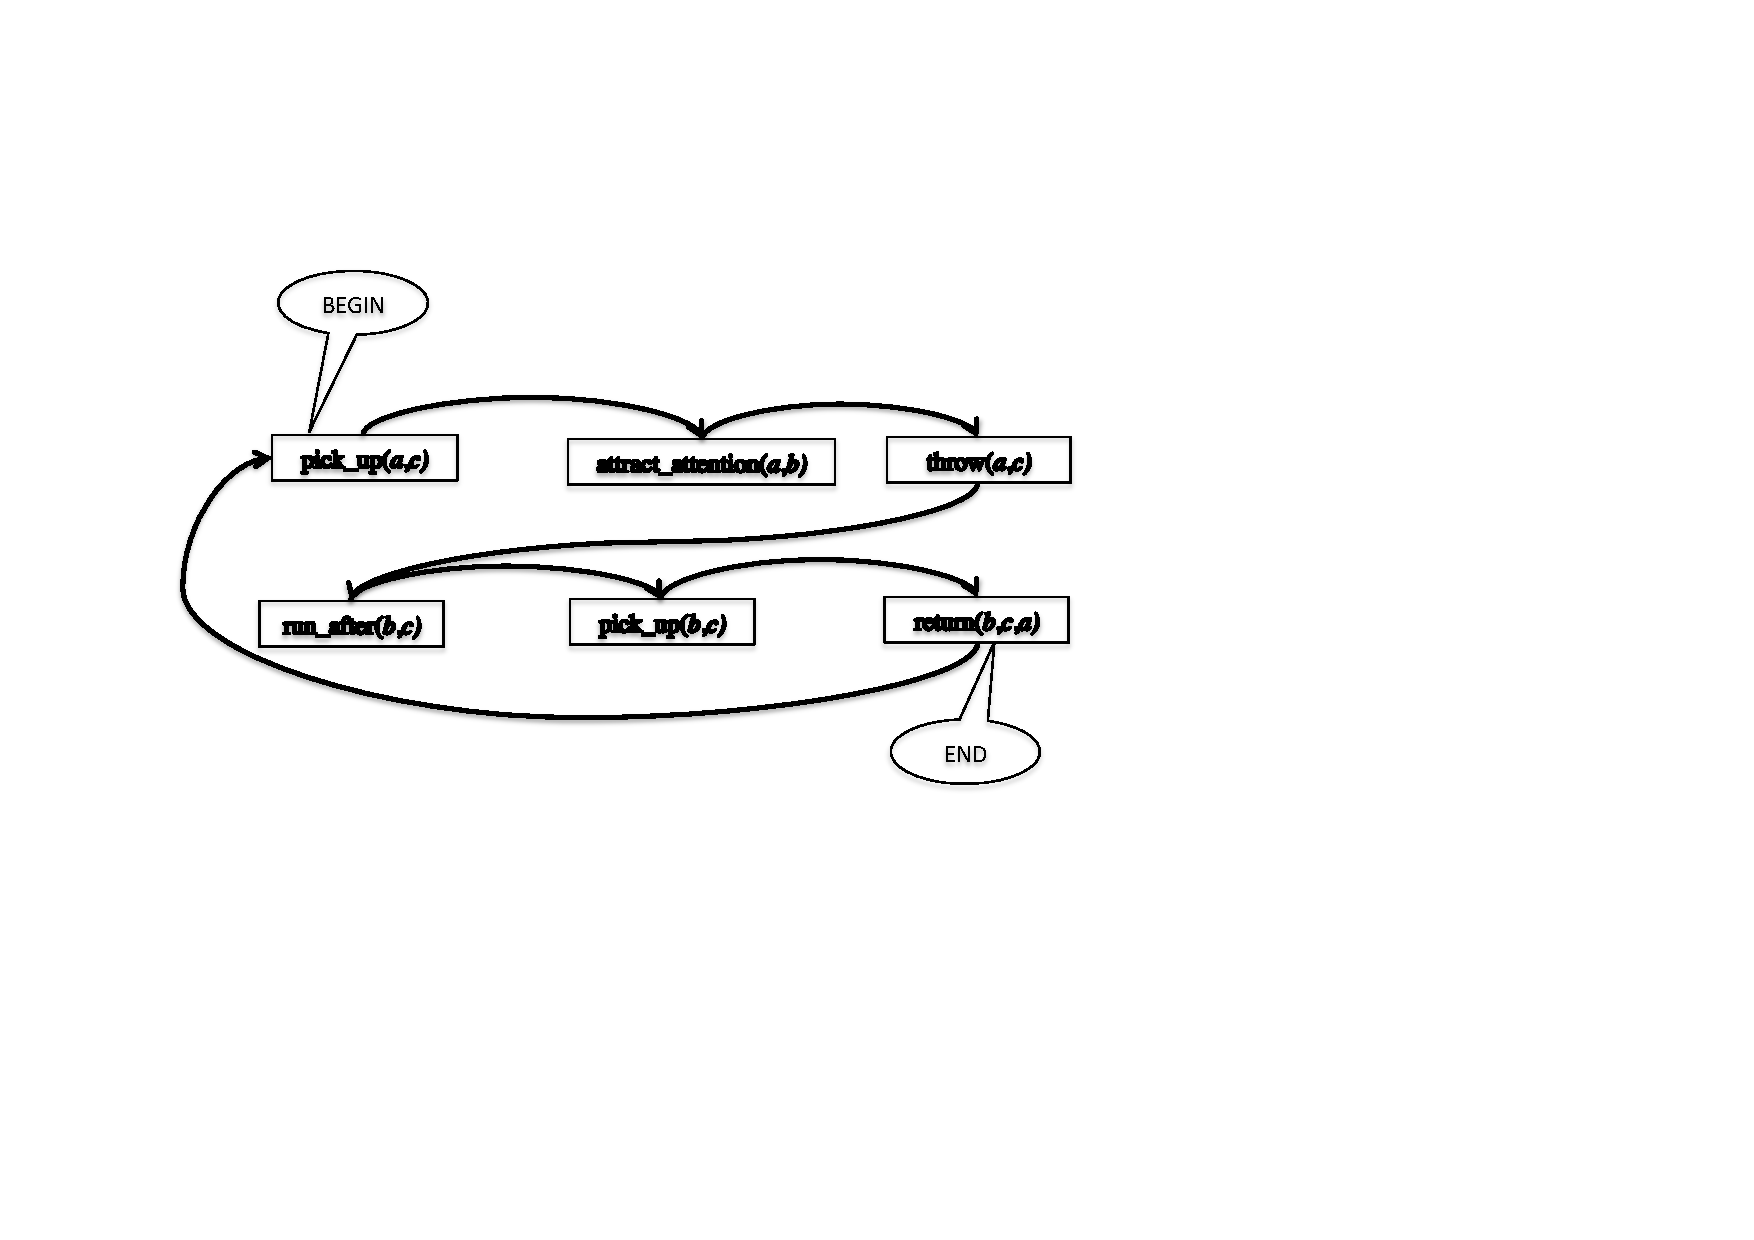
\includegraphics[width=6in]{fetch}

\hspace*{-4em}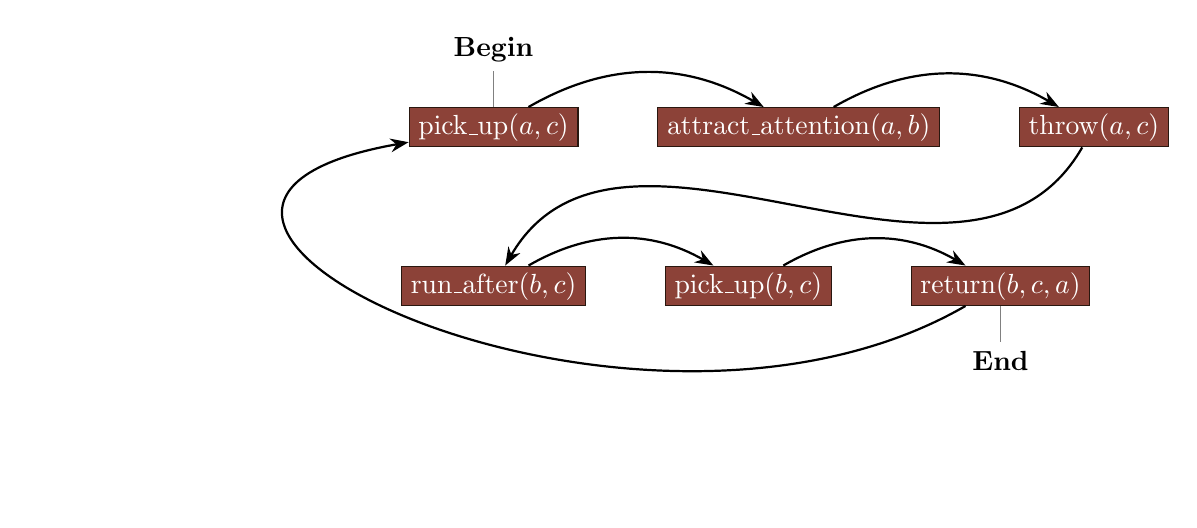
\begin{tikzpicture}[
  play/.style={rectangle, fill=Lamentation5, draw=Lamentation1, text=white, text depth=0.25ex, text height=1.5ex}
  ]

\node [play, pin=above:\textbf{Begin}] (p1) {pick\_up($a,c$)};
\node [play, right=of p1] (p2) {attract\_attention($a,b$)};
\node [play, right=of p2] (p3) {throw($a,c$)};
\node [play, below=1.5 of p1] (p4) {run\_after($b,c$)};
\node [play, right=of p4] (p5) {pick\_up($b,c$)};
\node [play, right=of p5, pin=below:\textbf{End}] (p6) {return($b,c,a$)};

\path [-{Stealth[]}, thick] 
(p1) edge [bend left] (p2)
(p2) edge [bend left] (p3)
(p3) edge [out=240, in=60] (p4)
(p4) edge [bend left] (p5)
(p5) edge [bend left] (p6)
(p6) edge [out=210, in=190, looseness=1.7] (p1);  
\end{tikzpicture}


\caption{play\_fetch($a$,$b$,$c$)}
\label{fig:fetch}
\end{figure}




   

In an important series of papers including
\cite{Fernando2004,Fernando2006,Fernando2008,Fernando2009,Fernando2011}, Fernando introduces a finite state
approach to event analysis where events are analyzed in terms of
finite state automata something like what we have represented in
Figure~\ref{fig:fetch-fs}.
\begin{figure} 

%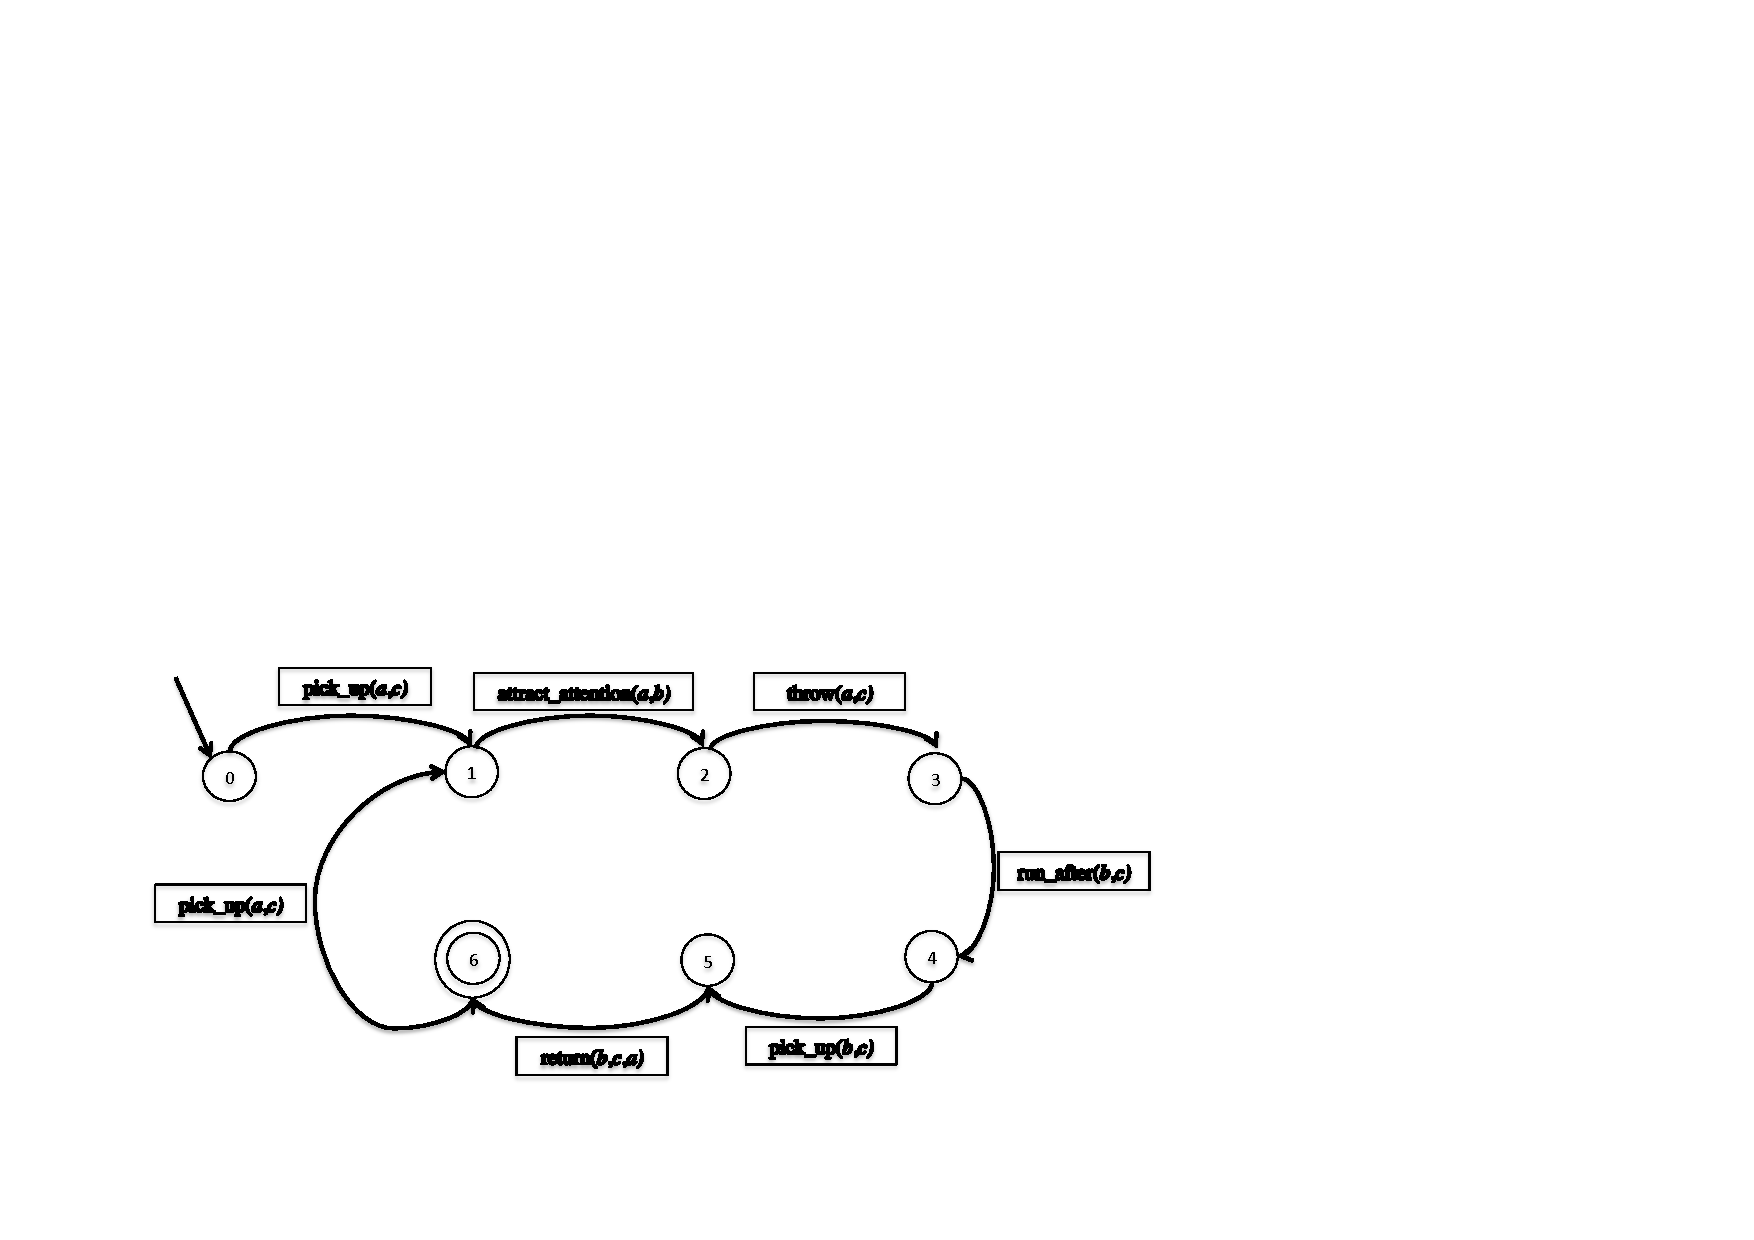
\includegraphics[width=6in]{fetch-fs}

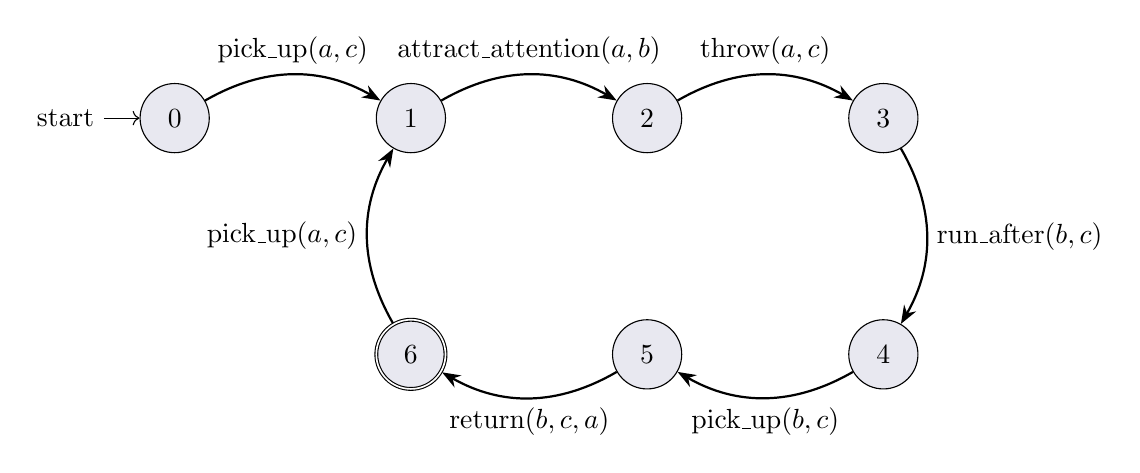
\begin{tikzpicture}[
  node distance=3cm, 
  on grid,
  every state/.style={fill=Lamentation2},
  ]

\node [state, initial] (n0) {0};
\node [state] (n1) [right=of n0] {1};
\node [state] (n2) [right=of n1] {2};
\node [state] (n3) [right=of n2] {3};
\node [state] (n4) [below=of n3] {4};
\node [state] (n5) [left=of n4] {5};
\node [state, accepting] (n6) [left=of n5] {6};

\path [-{Stealth[]}, thick] 
(n0) edge [bend left] node [above] {pick\_up($a,c$)} (n1)
(n1) edge [bend left] node [above] {attract\_attention($a,b$)} (n2)
(n2) edge [bend left] node [above] {throw($a,c$)} (n3)
(n3) edge [bend left] node [right] {run\_after($b,c$)} (n4)
(n4) edge [bend left] node [below] {pick\_up($b,c$)} (n5)
(n5) edge [bend left] node [below] {return($b,c,a$)} (n6)
(n6) edge [bend left] node [left] {pick\_up($a,c$)} (n1);
\end{tikzpicture}


\caption{play\_fetch($a$,$b$,$c$) as a finite state machine}
\label{fig:fetch-fs}
\end{figure}  
Such an automaton will recognize a string of
sub-events.  The idea is that our perception of complex events can be seen as strings of
punctual observations similar to the kind of sampling we are
familiar with from audio technology and digitization processing in
speech recognition.  Thus events can be analyzed as strings of smaller
events.  What we mean by a string is made precise in
Appendix~\ref{sec:regular}. Any object of any type can be part of a
string.  Any two objects (including strings themselves), $s_1$ and $s_2$, can be
\textit{concatenated} to form a string ${s_1}^{\frown}s_2$.  An
important property of concatenation is \textit{associativity}, that is
if we concatenate $s_1$ with $s_2$ and then concatenate the result
with $s_3$ we get the same string that we would obtain by
concatenating $s_2$ with $s_3$ and then concatenating $s_1$ with the
result.  In symbols: $({s_1}^{\frown}s_2)^{\frown}s_3 =
{s_1}^{\frown}({s_2}^{\frown}s_3)$.  For this reason we normally write
${s_1}^{\frown}{s_2}^{\frown}s_3$ (without the parentheses) or simply
$s_1s_2s_3$ if it is clear from the context that we mean this to be
string concatenation.  Following Fernando we will use these strings to
give us our notion of temporal order. 

Although we will present strings in this way, we will model them as
records \label{pg:stringsasrecords} with distinguished labels related to the natural numbers, 
t$_0$, t$_1$, \ldots (`t' for ``time'').  The field labelled t$_n$
will correspond to the $n$th place in the string.  Thus a string of
objects $a_1a_2a_3$
will be the record in \nexteg{}.
\begin{ex} 
\record{\field{t$_0$}{$a_1$} \\
        \field{t$_1$}{$a_2$} \\
        \field{t$_2$}{$a_3$}} 
\end{ex} 
The concatenation of \preveg{} with the string $a_4$, that is, \nexteg{a}, will
be \nexteg{b}.
\begin{ex} 
\begin{subex} 
 
\item \record{\field{t$_0$}{$a_4$}} 
 
\item  \record{\field{t$_0$}{$a_1$} \\
        \field{t$_1$}{$a_2$} \\
        \field{t$_2$}{$a_3$} \\
        \field{t$_3$}{$a_4$}}
 
\end{subex} 
   
\end{ex} 
We will continue to
represent strings for convenience in the traditional way but modelling
strings as records will become important when following paths in
records down to elements in strings.  We will use $s[n]$ to represent
the $n$th element in a string $s$ (where the first element in the
string is $s[0]$).  But in terms of the record notation
this is just a convenient abbreviation for $s$.t$_n$.    

Now let us build further on the
types that we have introduced so far to include string types. For any
two types, $T_1$ and $T_2$, we can form the type ${T_1}^{\frown}T_2$.
This is the type of strings $a^{\frown}b$ where $a:T_1$ and $b:T_2$.
The concatenation operation on types (just like that on objects) is
associative so we do not use parentheses when more than one type is
involved, e.g. ${T_1}^{\frown}{T_2}^{\frown}T_3$.

Let us return to Kim watching the boy, $a$, playing fetch with the
dog, $b$, using the stick, $c$. % over a time interval $t$
She
perceives the event as being of type play\_fetch($a$,$b$,$c$).
But what does it mean to be an event of this type?  Given our
concatenation types we can build a type which corresponds to most of
what we have sketched in Figure~\ref{fig:fetch}, namely \nexteg{}.
% (again ignoring time for the sake of simplification).
\begin{ex} 
pick\_up($a$,$c$)$^{\frown}$attract\_attention($a$,$b$)$^{\frown}$throw($a$,$c$)$^{\frown}$run\_after($b$,$c$)$^{\frown}$pick\_up($b$,$c$)$^{\frown}$return($b$,$c$,$a$) 
\end{ex} 
\preveg{} is a type corresponding to everything we have represented in
Figure~\ref{fig:fetch} except for the arrow which loops back from the
end state to the start state.    In order to get the loop into the event
type we will use a kind of type which introduces a Kleene-+.  In
standard notations for strings $s^+$ stands for a string consisting of
one or more occurrences of $s$.\footnote{This notation was introduced
  by the mathematician Stephen Kleene.}  We will adopt this into types
by saying that for any type $T$ there is also a type $T^+$ which is
the type of strings of objects of type $T$ containing one or more
members.  (See Appendix~\ref{sec:regular} for a more precise
definition.)  The type \nexteg{} will, then,
give us a type corresponding to the complete Figure~\ref{fig:fetch}
since it will be the type consisting of strings of one or more events
of the type \preveg{}.
\begin{ex} 
(pick\_up($a$,$c$)$^{\frown}$attract\_attention($a$,$b$)$^{\frown}$throw($a$,$c$)$^{\frown}$run\_after($b$,$c$)$^{\frown}$pick\_up($b$,$c$)$^{\frown}$
\\ return($b$,$c$,$a$))$^+$ 
\end{ex}


% In \preveg{} we simplified the string type by excluding time.  Now we
% will consider what is needed to put time back in.  Each of the
% subevents represented there is associated with a time interval, a
% different time interval for each subevent.  The type for time
% intervals, which we will abbreviate as \textit{TimeInt} is \nexteg{}\label{pg:TimeInt}.
% \begin{ex} 
% \record{\tfield{start}{\textit{Time}} \\
%         \tfield{end}{\textit{Time}} \\
%         \tfield{c$_<$}{start$<$end}}
% \end{ex} 
% where \textit{Time} is the type of time points and $<$ is the relation
% ``earlier than'' defined on the witnesses of this type.\footnote{We
%   use the infix notation $t_1<t_2$ rather than the official notation
%   $<(t_1,t_2)$.}  In order to get time intervals associated with each
% subevent we will treat the subevent types as record types rather than
% ptypes.  Thus as a first step towards characterizing the right type we
% have \nexteg{}.
% \begin{ex} 
% \smallrecord{\smalltfield{e-time}{\textit{TimeInt}} \\
%              \smalltfield{c$_{\mathrm{pick\_up}}$}{pick\_up($a$,$c$,e-time)}}$^{\frown}$\smallrecord{\smalltfield{e-time}{\textit{TimeInt}}
%              \\
%                   \smalltfield{c$_{\mathrm{attract\_attention}}$}{attract\_attention($a$,$b$,e-time)}}$^{\frown}$

% \medskip
% \smallrecord{\smalltfield{e-time}{\textit{TimeInt}} \\
%              \smalltfield{c$_{\mathrm{throw}}$}{throw($a$,$c$,e-time)}}$^{\frown}$\smallrecord{\smalltfield{e-time}{\textit{TimeInt}} \\
%              \smalltfield{c$_{\mathrm{run\_after}}$}{run\_after($b$,$c$,e-time)}}$^{\frown}$

% \medskip
% \smallrecord{\smalltfield{e-time}{\textit{TimeInt}} \\
%              \smalltfield{c$_{\mathrm{pick\_up}}$}{pick\_up($b$,$c$,e-time)}}$^{\frown}$\smallrecord{\smalltfield{e-time}{\textit{TimeInt}} \\
%              \smalltfield{c$_{\mathrm{return}}$}{return($b$,$c$,$a$,e-time) }}
% \end{ex}

% This will get us a time interval for each subevent but it does not
% require any relationship between the time intervals of the different
% subevents whereas, of course, each subevent should occur at a later
% time than the previous one.  In order to achieve this we will
% introduce a more restricted notion of type concatenation especially
% for record types which have a field
% \smallrecord{\smalltfield{e-time}{\textit{TimeInt}}} as in \nexteg{}.
% \begin{ex}
% \begin{enumerate} 
% \item If $T_1$ and $T_2$ are subtypes of
% \smallrecord{\smalltfield{e-time}{\textit{TimeInt}}}$^+$ then
% $T_1^{\frown_<}T_2$ is a type. 

% \item $a:T_1^{\frown_<}T_2$ iff $a=a_1^{\frown}a_2$, $a_1:T_1$, $a_2:T_2$ and
%   last($a_1$).e-time.end$<$first($a_2$).e-time.start
% \end{enumerate}
% \end{ex} 
% Here first($s$) and last($s$) pick out the first and last elements
% respectively of the string $s$.  We need to make a similar adjustment
% to the Kleene-+ type constructor.
% \begin{ex} 
% \begin{enumerate} 
 
% \item If $T$ is a subtype of
%   \smallrecord{\smalltfield{e-time}{\textit{TimeInt}}} then $T^{+_<}$
%   is a type
 
% \item $a:T^{+_<}$ iff $a=x_1^\frown\!\ldots^\frown\!x_n$, $n>0$ and
%   for $i$, $j$, $1\leq
% i<j\leq n$, $x_i:T$, $x_j:T$ and $x_i^{\frown}x_j:T^{\frown_<}T$ 
 
% \end{enumerate} 
   
% \end{ex} 

% [The details of temporal concatenation above should be included in the
% appendix.]

We will complicate \preveg{} slightly by substituting record types for
the ptypes as in \nexteg{}.  We do this because we
will want to allow for things happening simultaneously and record
types will give us a straightforward way of allowing this.
\begin{ex} 
(\smallrecord{\smalltfield{e}{pick\_up($a$,$c$)}}$^{\frown}$\smallrecord{\smalltfield{e}{attract\_attention($a$,$b$)}}$^{\frown}$\smallrecord{\smalltfield{e}{throw($a$,$c$)}}$^{\frown}$\smallrecord{\smalltfield{e}{run\_after($b$,$c$)}}$^{\frown}$\\
\smallrecord{\smalltfield{e}{pick\_up($b$,$c$)}}$^{\frown}$\smallrecord{\smalltfield{e}{return($b$,$c$,$a$)}})$^+$ 
\label{eg:fetch-type}
\end{ex}
The label `e' (``event'') occurs in each of the elements of the string
type.  In this case we will say that `e' labels a \textit{dimension}
of events of this type.  The `e'-dimension can be thought of as the
dimension which characterizes what is happening at each stage of the
event.  If you want to think geometrically, you can think of the
event-string as being located in a space of event types (that is, the ptypes).

% So now we can represent the event type for playing fetch as \nexteg{}.
% \begin{ex} 
% (\smallrecord{\smalltfield{e-time}{\textit{TimeInt}} \\
%              \smalltfield{c$_{\mathrm{pick\_up}}$}{pick\_up($a$,$c$,e-time)}}$^{\frown_<}$\smallrecord{\smalltfield{e-time}{\textit{TimeInt}}
%              \\
%                   \smalltfield{c$_{\mathrm{attract\_attention}}$}{attract\_attention($a$,$b$,e-time)}}$^{\frown_<}$

% \medskip
% \smallrecord{\smalltfield{e-time}{\textit{TimeInt}} \\
%              \smalltfield{c$_{\mathrm{throw}}$}{throw($a$,$c$,e-time)}}$^{\frown_<}$\smallrecord{\smalltfield{e-time}{\textit{TimeInt}} \\
%              \smalltfield{c$_{\mathrm{run\_after}}$}{run\_after($b$,$c$,e-time)}}$^{\frown_<}$

% \medskip
% \smallrecord{\smalltfield{e-time}{\textit{TimeInt}} \\
%              \smalltfield{c$_{\mathrm{pick\_up}}$}{pick\_up($b$,$c$,e-time)}}$^{\frown_<}$\smallrecord{\smalltfield{e-time}{\textit{TimeInt}} \\
%              \smalltfield{c$_{\mathrm{return}}$}{return($b$,$c$,$a$,e-time) }})$^{+_<}$
% \end{ex}

What happens when Kim perceives an event as being of this type?  She
makes a series of observations of events, assigning them to types in
the string type.  Note that the ptypes in each of the types can be
further broken down in a similar way.  This gives us a whole hierarchy
of perceived events which at some point have to bottom out in basic
perceptions which are not further analyzed.  In order to recognize an
event as being of this type Kim does not need to perceive a string of
events corresponding to each of the types in the string types.  She
may, for example, observe the boy waving the stick to attract the
dog's attention, get distracted by a bird flying overhead for a while,
and then return to the fetch event at the point where the dog is
running back to the boy with the stick.  This still enables her to
perceive the event as an event of fetch playing because she has seen
such events before and learned that such events are of the string type in \preveg{}.  It suffices for her to observe enough of the elements in
the string to distinguish the event from other event types she may
have available in her knowledge resources.  Suppose, for example, that
she has just two event string types available that begin with the picking
up of a stick by a human in the company of a dog.  One is \preveg{}.
The other is one that leads to the human beating the dog with the
stick.  If she only observes the picking up of the stick she cannot be
sure whether what she is observing is a game of fetch or a beating.
However, as soon as she observes something in the event string which
belongs only to the fetch type of string she can reasonably conclude
that she is observing an event of the fetch type.  She may, of course,
be wrong.  She may be observing an event of a type which she does not
yet have available in her resource of event types, in which case she
will need to learn about the new event type and add it to her
resources.  However, given the resources at her disposal she can make
a prediction about the nature of the rest of the event.  One could
model her prediction making ability in terms of a function which maps
a situation (modelled as a record) to a type of predicted situation,
for example \nexteg{}.
\begin{ex} 
$\lambda r$:\smallrecord{\smalltfield{x}{\textit{Ind}} \\
                         \smalltfield{c$_{\mathrm{human}}$}{human(x)}
                         \\
                         \smalltfield{y}{\textit{Ind}} \\
                         \smalltfield{c$_{\mathrm{dog}}$}{dog(y)} \\
                         \smalltfield{z}{\textit{Ind}} \\
                         \smalltfield{c$_{\mathrm{stick}}$}{stick(z)}
                         \\
                         \smalltfield{e}{\smallrecord{
             \smalltfield{e}{pick\_up(x,z)}}$^{\frown}$\smallrecord{
                  \smalltfield{e}{attract\_attention(x,y)}}}} .
            \\*[.75\baselineskip]
\hspace*{4em}\smallrecord{\smalltfield{e}{play\_fetch($r$.x,$r$.y,$r$.z)}
\\
\smalltfield{c$_{\mathrm{init}}$}{init($r$.e,e)}}
\label{ex:ev-predict-fun}
\end{ex} 
% \begin{ex} 
% $\lambda r$:\smallrecord{\smalltfield{x}{\textit{Ind}} \\
%                          \smalltfield{c$_{\mathrm{human}}$}{human(x)}
%                          \\
%                          \smalltfield{y}{\textit{Ind}} \\
%                          \smalltfield{c$_{\mathrm{dog}}$}{dog(y)} \\
%                          \smalltfield{z}{\textit{Ind}} \\
%                          \smalltfield{c$_{\mathrm{stick}}$}{stick(z)}
%                          \\
%                          \smalltfield{e-time}{\textit{TimeInt}} \\
%                          \smalltfield{e}{\smallrecord{\smalltfield{e-time}{\textit{TimeInt}}
%                              \\
% \smalltfield{c$_{\leq}$}{$\Uparrow$e-time.start$\leq$e-time.start} \\
%              \smalltfield{c$_{\mathrm{pick\_up}}$}{pick\_up($\Uparrow$x,$\Uparrow$z,e-time)}}$^{\frown_<}$\smallrecord{\smalltfield{e-time}{\textit{TimeInt}}
%              \\
% \smalltfield{c$_{\leq}$}{e-time.start$\leq\Uparrow$e-time.start} \\
%                   \smalltfield{c$_{\mathrm{attract\_attention}}$}{attract\_attention($\Uparrow$x,$\Uparrow$y,e-time)}}}}
%             \\*[.75\baselineskip]
% \hspace*{4em}(\smallrecord{\smalltfield{e-time}{\textit{TimeInt}} \\
%                            \smalltfield{c$_{\leq}$}{$r$.e-time.start$\leq$e-time.start} \\
%                            \smalltfield{e}{play\_fetch($r$.x,$r$.y,$r$.z,e-time)}})
% \label{ex:ev-predict-fun}
% \end{ex}

Here the predicate `init' has arity
$\langle$\textit{String}, \textit{String}$\rangle$.  The type init($s_1$,$s_2$) is
non-empty just in case $s_1$ is an initial substring of $s_2$.  We
achieve this by defining
\begin{quote}
If $s_1$ is a string of length $n$ and $s_2$ is a string of any
length, then $s$ : init($s_1$,$s_2$) iff the length of $s_2$ is
greater than or equal to $n$ and for each $i$, $0\leq i<n$,
$s_1[i]=s_2[i]$ and $s=s_2$.
\end{quote}
That is, if the initial substring condition holds then the second
argument to the predicate (and nothing else) is of the ptype.

% Here a `$\Uparrow$' prefixed to a path-name consisting of labels such
% as `e-time.start' or `x' means that the path-name is to start in the
% next higher record type in which the current record type is embedded.
% This notation is an abbreviation for something much less readable (but
% more precise) which is given in Appendix~\ref{app:rectypes}. [????
% This notation needs to be added to the appendix.]

The kind of function of which \preveg{} is an instance is a function
of the general form \nexteg{}.
\begin{ex} 
$\lambda a\!:\!T_1\ .\ T_2(a)$
\label{ex:deptypefun} 
\end{ex} 
where we use the notation $T_2(a)$ to represent the fact that $T_2$
depends on $a$. The nature of this dependence in
(\ref{ex:ev-predict-fun}) is seen in the occurrences of $r$ in the body
of the function, for example, `play\_fetch($r$.x,$r$.y,$r$.z)'.
Such a function maps an object of some type (represented by $T_1$) to
a type (represented by $T_2(a)$).  The type that results from an
application of this function will depend on what object it is applied
to -- that is, we have the possibility of obtaining different types
from different objects. In type theory such a function is often called
a \textit{dependent type}.  These functions will play an important
role in much of what is to come later in this book.  They will show up
many times in what appear at first blush to be totally unrelated
phenomena.  We want to suggest, however, that all of the phenomena we
will describe using such functions have their origin in our basic
cognitive ability to make predictions on the basis of partial
observation of objects and events.

What happens when Kim does not observe enough of the event to be able
to predict with any certainty that the complete event will be a game
of fetch?  One theory would be that she can only make categorical
judgements, and that she has to wait until she has seen enough so that
there is only one type that matches in the collection of situation
types in her resources.  Another theory would be
one where she predicts a disjunction of the available matching types when there is
more than one that matches.  One might refine this theory so that she
can choose one of the available types but assign it a probability
based on the number of matching types.  If $n$ is the number of
matching types the probability of any one of them might be
$\frac{1}{n}$.  This assumes that each of the types is equally likely
to be realized.  It would be natural to assume, however, that the
probability which Kim assigns to any one of the matching types would
be dependent on her previous experience.  Suppose, for example, that
she has seen 100 events of a boy picking up a stick in the company of
a dog, 99 of those events led to a game of fetch and only one led to
the boy beating the dog.  One might then assume that when she now sees
the boy pick up the stick she would assign a 99\% probability to the
type of fetch events and only 1\% probability to the boy beating the
dog.  That is, the probability she assigns to an event of a boy
picking up a stick leading to a game of fetch is the result of
dividing the number of instances of a game of fetch she has already
observed by the sum of the number of instances she has observed of any types whose
initial segment involves the picking up of a stick.  In more general
terms we can compute the probability which an agent $A$ assigns on the
basis of a string, $\omega$, of previous observations to a
predicted type $T_{\mathit{pr}}$ given an observed type $T_{\mathit{obs}}$, $P_{A,\omega}(T_{\mathit{pr}}\mid T_{\mathit{obs}})$, in the case where
$T_{\mathit{pr}}$ is a member of the set of alternatives which can be
predicted from $T_{\mathit{obs}}$ according to $A$'s resources based on $\omega$,
$\mathrm{alt}_{A,\omega}(T_{\mathit{obs}})$, by the following formula:
\[P_{A,\omega}(T_{\mathit{pr}}\mid T_{\mathit{obs}}) =
\frac{\mid\{T_{\mathit{pr}}\}^{A,\omega}\mid}{\sum\limits_{T_{\mathit{alt}}\in\mathrm{alt}_{A,\omega}(T_{\mathit{obs}})}\mid\{T_{\mathit{alt}}\}^{A,\omega}\mid}\]
where $\{T\}^{A,\omega}$ is the set of objects of type $T$ observed by $A$
in $\omega$.  If $T_{\mathit{pr}}$ is not a member of
$\mathrm{alt}_{A,\omega}(T_{\mathit{obs}})$, that is not one of the
alternatives, we say that $P_{A,\omega}(T_{\mathit{pr}}\mid
T_{\mathit{obs}}) = 0$.

While this is still a rather naive and simple view of how
probabilities might be assigned it is not without interest, as shown
by the following points:  
\paragraph{Probability distributions} It will always provide a probability distribution over sets
of alternatives, that is,
\[\sum\limits_{T_{\mathit{pr}}\in\mathrm{alt}_{A,\omega}(T_{\mathit{obs}})}P_{A,\omega}(T_{\mathit{pr}}\mid
T_{\mathit{obs}}) = 1\]
\paragraph{Alternatives} We have assumed a notion of alternatives based on types of completed
events for which the observed event is an initial segment but other
notions of alternativeness could be considered and perhaps even
combined.  
\paragraph{Relativity of probability assignments} The notion of
probability is both agent and resource relative.  It represents the
probability which an agent will assign to a type when observing a
given situation after a previous string of observations.  Two agents may assign different
probabilities depending on the resources they have available.
\paragraph{Learning} Relevant observations will update the probability
distributions an agent will assign to a given set of alternatives
since the probability is computed on the basis of previous
observations of the alternative types.

Kim is not alone in being able to draw conclusions based on partial
observations of an event.  The dog can do it too.  As soon as the boy
has raised the stick and attracted the dog's attention the dog is
excitedly snapping at the stick and starting to run in the direction
in which the boy seems to be about to throw.  The dog also seems to be
attuned to string types of events just as Kim is and also able to make
predictions on the basis of partial observations.  The types to which
a dog is attuned will not be the same as those to which humans can be
attuned and this can certainly lead to miscommunication between humans
and dogs.  For example, there may be many reasons why I would go to
the place where outdoor clothes are hanging and where the dog's lead
is kept.  Many times it will be because I am planning to take the dog
out for a walk, but not as often as the dog appears to think, judging
from the excitement he shows any time I go near the lead.  It is
difficult to explain to the dog that I am just looking for a receipt
that I think I might have left in my coat pocket.  But the basic
mechanism of being able to assemble types of events
into string types of more complex events and make predictions on the
basis of these types seems to be common to both humans and dogs and a
good number of other animals too.  Perhaps simple organisms do not
have this ability and can only react to events that have already
happened, but not to predicted outcomes.

This basic inferential ability is thus not parasitic on the ability to
communicate using a human language.  It is, however, an ability which
appears to be exploited to a great extent in our use of language as we
will see in later chapters.  In the remaining sections of this chapter
we will look at some aspects of the type theory which seem more likely
to
correspond to cognitive abilities which only humans have.


% When talking about the intuition behind this
% analysis Fernando sometimes refers to strings of frames in a movie
% (e.g. in \cite{Fernando2008}).  But in many cases what he is calling
% a movie frame 
% can also be seen as a frame in something like the sense of frame semantics as well.

\section{Doing things with types}
\label{sec:typeacts}

The boy and the dog have to coordinate and interact in order to create an
event of the game of fetch.  This involves doing more with types than
just making judgements.  For example, when the dog observes the
situation in which the boy raises the stick, it may not be clear
to the dog whether this is part of a fetch-game situation or a
stick-beating situation.  The dog may be in a situation of
entertaining these two types as possibilities prior to making the
judgement that the situation is of the fetch type.  We will call this
act a query as opposed to a judgement.  Once the dog has made the
judgement that what it has observed so far is an initial segment of a
fetch type situation it has to make its own contribution in order to
realize the fetch type, that is, it has to run after the stick and
bring it back.  This involves the creation of a situation of a certain
type.  Thus creation acts are another kind of act related to types.
Creating objects of a given type often has a \textit{de se}
\citep[see, for example,][]{Perry1979,Lewis1979a,Ninan2010,Schlenker2011} aspect.  The dog
has to know that it itself must run after the stick in order to make
this a situation in which it and the boy are playing fetch.  There is
something akin to what Perry calls an essential indexical here,
though, of course, the dog does not have indexical linguistic
expressions. It is nevertheless part of the basic competence that an
agent needs in order to be able to coordinate its action with the rest
of the world that it has a primitive sense of self which is distinct
from being able to identify an object which has the same properties as
itself.  We will follow Lewis in modelling \textit{de se} in terms of
functional abstraction over the ``self''.  In our terms this will mean
that \textit{de se} type acts involve dependent types.

In standard type theory we have judgements such as $o:T$ ``$o$ is of type $T$'' 
and 
$T$ \textit{true} ``there is something of type $T$''.    We want to
enhance this notion of judgement by including a reference to the agent
$A$ which makes the judgement, giving judgements such as
$o:_AT$ ``agent $A$ judges that $o$ is of type $T$''
and 
$:_AT$ ``agent $A$ judges that there is some object of type $T$''. We will call
the first of these a \textit{specific} judgement and the second a
\textit{non-specific} judgement.  Such
judgements are one of the three kinds of acts represented in \nexteg{}
that we want to include
in our type act theory.
\begin{ex} 
\textit{Type Acts}
\begin{description}
\item[judgements] \mbox{}

\begin{description}
\item[\textit{specific}] $o:_A T$ ``agent $A$ judges object $o$ to be of type
  $T$''

\item[\textit{non-specific}] $:_A T$ ``agent $A$ judges that there is some
  object of type $T$''
\end{description}

\item[queries] \mbox{}
\begin{description}
\item[\textit{specific}] $o:_A T?$ ``agent $A$ wonders whether object $o$ is of type
  $T$''

\item[\textit{non-specific}] $:_A T?$ ``agent $A$ wonders whether there is some object of type
$T$''
\end{description}
\item[creations] \mbox{}
\begin{description}
\item[\textit{non-specific}] $:_A T!$ ``agent $A$ creates something of type
  $T$''
\end{description}
\end{description}

\end{ex} 
Note that creations only come in the non-specific variant.  You cannot
create an object which already exists.  

Creations are also limited in
that there are certain types which a given agent is not able to
realize as the main actor.  Consider for example the event type involved in the fetch
game of the dog running after the stick.  The human cannot be the main
creator of such
an event since it is the dog who is the actor.  The most the human can
do is wait until the dog has carried out the action
and we will count this as a creation type act.  This will become
important when we discuss coordination in the fetch-game below.  It is
actually important that the human makes this passive contribution to
the creation of the event of the dog running after the stick and does
not, for example, get the game confused by immediately throwing
another stick before the dog has had a chance to retrieve the first
stick.  There are other cases of event types which require a less
passive contribution from an agent other than the main actor.
Consider the type of event where the dog returns the stick to the
human.  The dog is clearly the main actor here but the human has also
a role to play in making the event realized.  For example, if the
human turns her back on the dog and ignores what is happening or runs
away the event type will not be realized despite the dog's best
efforts.  Other event types, such as lifting a piano, involve more
equal collaboration between two or more agents, where it is not
intuitively clear that any one of the agents is the main actor.  So
when we say ``agent $A$ creates something of type $T$'' perhaps it
would be more accurate to phrase this as ``agent $A$ contributes to
the creation of something of type $T$'' where $A$'s contribution might
be as little as  not realizing any of the other types involved in the game until
$T$ has been realized.   
   
\textit{De se} type acts involve functions which have the agent in its
domain and return a type, that is, they are dependent types which,
given the agent, will yield a type.  We will say that agents are of
type \textit{Ind} and that the relevant dependent types, 
$\mathcal{T}$, are functions of type
  (\textit{Ind}$\rightarrow$\textit{Type}).  
We characterize \textit{de se} type acts in a way parallel to
\preveg{}, as given in \nexteg{}.
\begin{ex}
\textit{De Se Type Acts} 
\begin{description}
\item[\textit{judgements}] \mbox{}
\begin{description}
\item[\textit{specific}]  $o:_A \mathcal{T}(A)$ ``agent $A$ judges object $o$ to be of type
  $\mathcal{T}(A)$''
\item[\textit{non-specific}] $:_A \mathcal{T}(A)$ ``agent $A$ judges
  that there is some object of type $\mathcal{T}(A)$''
\end{description}

\item[\textit{queries}] \mbox{}
\begin{description}
\item[\textit{specific}] $o:_A \mathcal{T}(A)?$ ``agent $A$ wonders whether object $o$ is of type
  $\mathcal{T}(A)$''
\item[\textit{non-specific}] $:_A \mathcal{T}(A)?$ ``agent $A$ wonders whether there is some object of type
$\mathcal{T}(A)$''
\end{description}

\item[\textit{creations}] \mbox{}
\begin{description}
\item[\textit{non-specific}] $:_A \mathcal{T}(A)!$ ``agent $A$ creates
  something of type $\mathcal{T}(A)$''
\end{description}
\end{description} 
\end{ex} 

From the point of view of the type theory \textit{de se} type acts
seem more complex than non-\textit{de se} type acts since they involve
a dependent rather than a non-dependent type and a functional
application of that dependent type to the agent.  However, from a
cognitive perspective one might expect \textit{de se} type acts to be
more basic.  Agents which perform type acts using types directly
related to themselves are behaving egocentrically and one could regard
it as a more advanced level of abstraction to consider types which are
independent of the agent.  This seems a puzzling way in which our
notions of type seem in conflict with out intuitions about cognition.   

While these type acts are prelinguistic (we need them to account for
the dog's behaviour in the game of fetch) we will try to argue later
that they are the basis on which the notion of speech act
\citep{Austin1962,Searle1969} is built.  Our notion of using types in
query acts seems intuitively related to work on inquisitive semantics
\citep{GroenendijkRoelofsen2012} where some propositions (in
particular disjunctions) are regarded as inquisitive.  However, this
will still allow us to make a distinction between questions and
assertions in natural language as argued for by \cite{Ginzburg2012}.

Let us now apply these notions to the kind of interaction that has to
take place between the human and the dog in a game of fetch.  First
consider in more detail what is actually involved in playing a game of
fetch, that is creating an event of type (\ref{eg:fetch-type}).  Each
agent has to keep track in some way of where they are in the game and
in particular what needs to happen next.  We analyze this by saying
that each agent has an information state which we will model as a
record.  We need to keep track of the progression of types of
information state for an agent during the course of the game.  We will
refer to the types of information states as gameboards.\footnote{Our
  notions of \textit{information state} and \textit{gameboard} are
  taken from \cite{Larsson2002} and \cite{Ginzburg2012} respectively
  as well as a great deal of related literature on the gameboard or
  information state approach to dialogue analysis originating from
  \cite{Ginzburg1994}.  We have adapted the notions somewhat to our own
  purposes and will take this up in more detail in
  Chapter~\ref{ch:infex}.}  The idea is that as part of the event
occurs then the agent's gameboard is updated so that an event of the
next type in the string is expected.  For now, we will consider
gameboards which only place one requirement on information states,
namely that there is an agenda which indicates the type of the next
move in the game.  Thus if the agent is playing fetch and observes an
event of the type where the human throws the stick, then, according to
(\ref{eg:fetch-type}), the next move in the game will be an event of
the type where the dog runs after the stick.  If the actor in the next
move is the agent herself then the agent will need to create an event
of the type of the next move if the game is to progress.  If the actor in the next move is the
other player in the game, then the agent will need to observe an event
and judge it to be of the appropriate type in order for the game to
progress.  The type of information states, \textit{InfoState}, will be
\nexteg{a}.  (In Chapter~\ref{ch:infex}, when we apply these ideas to dialogue, we
will see more complex information states.)  The type of the initial
information state, \textit{InitInfoState}, will be one where the agenda is required to be the
empty list.
\begin{ex}
\begin{subex} 
\item \record{\tfield{agenda}{[\textit{RecType}]}}
\item \record{\mfield{agenda}{[]}{[\textit{RecType}]}} 
\end{subex}
\end{ex} 
We can now see the rules of the game corresponding to the type
(\ref{eg:fetch-type}) as a set of update functions which indicate for
an information state of a given type what type the next information
state may belong to if an event of a certain type occurs.  These
update functions correspond to the transitions in a finite state
machine.  This is
given in \nexteg{}.
\begin{ex} 
\{ \begin{tabular}[t]{l}
$\lambda
  r$:\smallrecord{\smallmfield{agenda}{[]}{[\textit{RecType}]}} . \\
\hspace*{1em}\smallrecord{\smallmfield{agenda}{[\smallrecord{\smalltfield{e}{pick\_up($a$,$c$)}}]}{[\textit{RecType}]}},
\\ 
$\lambda
r$:\smallrecord{\smallmfield{agenda}{[\smallrecord{\smalltfield{e}{pick\_up($a$,$c$)}}]}{[\textit{RecType}]}}
\\
\hspace*{1em}$\lambda
e$:\smallrecord{\smalltfield{e}{pick\_up($a$,$c$)}} . \\
\hspace*{2em}\smallrecord{\smallmfield{agenda}{[\smallrecord{\smalltfield{e}{attract\_attention($a$,$b$)}}]}{[\textit{RecType}]}},
\\
$\lambda
r$:\smallrecord{\smallmfield{agenda}{[\smallrecord{\smalltfield{e}{attract\_attention($a$,$b$)}}]}{[\textit{RecType}]}}
\\
\hspace*{1em}$\lambda
e$:\smallrecord{\smalltfield{e}{attract\_attention($a$,$b$)}} . \\
\hspace*{2em}\smallrecord{\smallmfield{agenda}{[\smallrecord{\smalltfield{e}{throw($a$,$c$)}}]}{[\textit{RecType}]}},
\\
$\lambda
r$:\smallrecord{\smallmfield{agenda}{[\smallrecord{\smalltfield{e}{throw($a$,$c$)}}]}{[\textit{RecType}]}}
\\
\hspace*{1em}$\lambda
e$:\smallrecord{\smalltfield{e}{throw($a$,$c$)}} . \\
\hspace*{2em}\smallrecord{\smallmfield{agenda}{[\smallrecord{\smalltfield{e}{run\_after($b$,$c$)}}]}{[\textit{RecType}]}},
\\
$\lambda
r$:\smallrecord{\smallmfield{agenda}{[\smallrecord{\smalltfield{e}{run\_after($b$,$c$)}}]}{[\textit{RecType}]}}
\\
\hspace*{1em}$\lambda
e$:\smallrecord{\smalltfield{e}{run\_after($b$,$c$)}} . \\
\hspace*{2em}\smallrecord{\smallmfield{agenda}{[\smallrecord{\smalltfield{e}{pick\_up($b$,$c$)}}]}{[\textit{RecType}]}},
\\
$\lambda
r$:\smallrecord{\smallmfield{agenda}{[\smallrecord{\smalltfield{e}{pick\_up($b$,$c$)}}]}{[\textit{RecType}]}}
\\
\hspace*{1em}$\lambda
e$:\smallrecord{\smalltfield{e}{pick\_up($b$,$c$)}} . \\
\hspace*{2em}\smallrecord{\smallmfield{agenda}{[\smallrecord{\smalltfield{e}{return($b$,$c$,$a$)}}]}{[\textit{RecType}]}},
\\
$\lambda
r$:\smallrecord{\smallmfield{agenda}{[\smallrecord{\smalltfield{e}{return($b$,$c$,$a$)}}]}{[\textit{RecType}]}}
\\
\hspace*{1em}$\lambda
e$:\smallrecord{\smalltfield{e}{return($b$,$c$,$a$)}} . \\
\hspace*{2em}\smallrecord{\smallmfield{agenda}{[]}{[\textit{RecType}]}}
\\
% $\lambda
% r$:\smallrecord{\smallmfield{agenda}{[\smallrecord{\smalltfield{e}{return($b$,$c$,$a$)}}]}{[\textit{RecType}]}}
% \\
% \hspace*{1em}$\lambda
% e$:\smallrecord{\smalltfield{e}{return($b$,$c$,$a$)}} . \\
% \hspace*{2em}\smallrecord{\smallmfield{agenda}{[\smallrecord{\smalltfield{e}{[pick\_up($a$,$c$)]}}]}{[\textit{RecType}]}}
 \end{tabular} \\
\hspace*{\textwidth} \} 
\label{eg:fetch-update-funs} 
 
   
\end{ex} 

Since we are treating an empty agenda as the condition for the input
to the initial state in the corresponding automaton and also the
output of the final state we automatically get the loop effect from
the final state to the initial state.  In order to prevent the loop we
would have to distinguish the type corresponding to the initial and
final states. Note that the functions in \preveg{} are of the
type \nexteg{}.
\begin{ex}
(\smallrecord{\smalltfield{agenda}{[\textit{RecType}]}}$\rightarrow$(\textit{Rec}$\rightarrow$\textit{RecType}))
\end{ex}
That is, they map an information state containing an agenda (modelled
as a record containing an agenda field) and an
event (modelled as a record) to a record type.   This is true of all
except for the function corresponding to the initial state which is of
type \nexteg{}.
\begin{ex}
(\smallrecord{\smalltfield{agenda}{[\textit{RecType}]}}$\rightarrow$\textit{RecType})
\end{ex}
That is, it maps an information state directly to a record type and does not
require an event.  We can think of this set as the set of rules which
define the game.  It is of the type \nexteg{}.
\begin{ex}
\{((\smallrecord{\smalltfield{agenda}{[\textit{RecType}]}}$\rightarrow$(\textit{Rec}$\rightarrow$\textit{RecType}))$\vee$(\smallrecord{\smalltfield{agenda}{[\textit{RecType}]}}$\rightarrow$\textit{RecType}))\}
\end{ex}
Let us call the type in \preveg{} \textit{GameRules}.  Sets of game
rules of this type define the rules for specific participants as in
(\ref{eg:fetch-update-funs}).  In order to characterize the game in
general we need to abstract out the roles of the individual
participants in the game.  This we will do by defining a function from
a record containing individuals appropriate to play the roles in the
game thus revising (\ref{eg:fetch-update-funs}) to \nexteg{}.

\begin{ex}
$\lambda r^*$:\record{\tfield{h}{\textit{Ind}} \\
                          \tfield{c$_{\mathrm{human}}$}{human(h)} \\
                          \tfield{d}{\textit{Ind}} \\
                          \tfield{c$_{\mathrm{dog}}$}{dog(d)} \\
                          \tfield{s}{\textit{Ind}} \\
                          \tfield{c$_{\mathrm{stick}}$}{stick(s)}}
                        . \\ 
\hspace*{1em}\{ \begin{tabular}[t]{l}
$\lambda
  r$:\smallrecord{\smallmfield{agenda}{[]}{[\textit{RecType}]}} . \\
\hspace*{1em}\smallrecord{\smallmfield{agenda}{[\smallrecord{\smalltfield{e}{pick\_up($r^*$.h,$r^*$.s)}}]}{[\textit{RecType}]}},
\\ 
$\lambda
r$:\smallrecord{\smallmfield{agenda}{[\smallrecord{\smalltfield{e}{pick\_up($r^*$.h,$r^*$.s)}}]}{[\textit{RecType}]}}
\\
\hspace*{1em}$\lambda
e$:\smallrecord{\smalltfield{e}{pick\_up($r^*$.h,$r^*$.s)}} . \\
\hspace*{2em}\smallrecord{\smallmfield{agenda}{[\smallrecord{\smalltfield{e}{attract\_attention($r^*$.h,$r^*$.d)}}]}{[\textit{RecType}]}},
\\
$\lambda
r$:\smallrecord{\smallmfield{agenda}{[\smallrecord{\smalltfield{e}{attract\_attention($r^*$.h,$r^*$.d)}}]}{[\textit{RecType}]}}
\\
\hspace*{1em}$\lambda
e$:\smallrecord{\smalltfield{e}{attract\_attention($r^*$.h,$r^*$.d)}} . \\
\hspace*{2em}\smallrecord{\smallmfield{agenda}{[\smallrecord{\smalltfield{e}{throw($r^*$.h,$r^*$.s)}}]}{[\textit{RecType}]}},
\\
$\lambda
r$:\smallrecord{\smallmfield{agenda}{[\smallrecord{\smalltfield{e}{throw($r^*$.h,$r^*$.s)}}]}{[\textit{RecType}]}}
\\
\hspace*{1em}$\lambda
e$:\smallrecord{\smalltfield{e}{throw($r^*$.h,$r^*$.s)}} . \\
\hspace*{2em}\smallrecord{\smallmfield{agenda}{[\smallrecord{\smalltfield{e}{run\_after($r^*$.d,$r^*$.s)}}]}{[\textit{RecType}]}},
\\
$\lambda
r$:\smallrecord{\smallmfield{agenda}{[\smallrecord{\smalltfield{e}{run\_after($r^*$.d,$r^*$.s)}}]}{[\textit{RecType}]}}
\\
\hspace*{1em}$\lambda
e$:\smallrecord{\smalltfield{e}{run\_after($r^*$.d,$r^*$.s)}} . \\
\hspace*{2em}\smallrecord{\smallmfield{agenda}{[\smallrecord{\smalltfield{e}{pick\_up($r^*$.d,$r^*$.s)}}]}{[\textit{RecType}]}},
\\
$\lambda
r$:\smallrecord{\smallmfield{agenda}{[\smallrecord{\smalltfield{e}{pick\_up($r^*$.d,$r^*$.s)}}]}{[\textit{RecType}]}}
\\
\hspace*{1em}$\lambda
e$:\smallrecord{\smalltfield{e}{pick\_up($r^*$.d,$r^*$.s)}} . \\
\hspace*{2em}\smallrecord{\smallmfield{agenda}{[\smallrecord{\smalltfield{e}{return($r^*$.d,$r^*$.s,$r^*$.h)}}]}{[\textit{RecType}]}},
\\
$\lambda
r$:\smallrecord{\smallmfield{agenda}{[\smallrecord{\smalltfield{e}{return($r^*$.d,$r^*$.s,$r^*$.h)}}]}{[\textit{RecType}]}}
\\
\hspace*{1em}$\lambda
e$:\smallrecord{\smalltfield{e}{return($r^*$.d,$r^*$.s,$r^*$.h)}} . \\
\hspace*{2em}\smallrecord{\smallmfield{agenda}{[]}{[\textit{RecType}]}}
\\
% $\lambda
% r$:\smallrecord{\smallmfield{agenda}{[\smallrecord{\smalltfield{e}{return($b$,$c$,$a$)}}]}{[\textit{RecType}]}}
% \\
% \hspace*{1em}$\lambda
% e$:\smallrecord{\smalltfield{e}{return($b$,$c$,$a$)}} . \\
% \hspace*{2em}\smallrecord{\smallmfield{agenda}{[\smallrecord{\smalltfield{e}{[pick\_up($a$,$c$)]}}]}{[\textit{RecType}]}}
 \end{tabular} \\
\hspace*{\textwidth} \} 
\end{ex}
\preveg{} is of type (\textit{Rec}$\rightarrow$\textit{GameRules})
which we will call \textit{Game}. 
  
Specifying the rules of the game in terms of update functions in this way will not actually getting
anything to happen, though.  For that we need type acts of the kind we
discussed. We link the update functions to type acts by means of
\textit{licensing conditions on type acts}.  A basic licensing
condition is that an agent can create (or contribute to the creation
of) a witness for the first type that occurs on the agenda in its
information state.  Such a licensing condition is expressed in
\nexteg{}.
\begin{ex} 
If $A$ is an agent, $s_i$ is $A$'s current information state, \\ $s_i
:_A$ \record{\mfield{agenda}{$T\!\mid\!
    R\ $}{[\textit{RecType}]}}, then $:_A T!$ is licensed. 
\end{ex}
(Here we use the notation $T\!\mid\!R$ to represent a list whose first
member is $T$ and whose rest is $R$.  For example, if the list is
$[T_1,T_2,T_3]$ then $T$ would correspond to $T_1$ and $R$ would
correspond to $[T_2,T_3]$. See Appendix~\ref{app:listtypes}.) 

Update functions of the kind we have discussed are handled by the
licensing conditions in \nexteg{}.
\begin{ex} 
\begin{subex} 
 
\item If $f:(T_1\rightarrow(T_2\rightarrow\textit{Type}))$ is an update
function, $A$ is an agent, $s_i$ is $A$'s current information state,
$s_i:_A T_i$, $T_i\sqsubseteq T_1$ (and $s_i:T_1$), then an event $e:_A
T_2$ (and $e:T_2$) licenses $s_{i+1}:_A f(s_i)(e)$. 
 
\item If $f:(T_1\rightarrow(T_2\rightarrow\textit{Type}))$ is an update
function, $A$ is an agent, $s_i$ is $A$'s current information state,
$s_i:_A T_i$, $T_i\sqsubseteq T_1$ (and $s_i:T_1$), $s_{i+1}:_A
f(s_i)$ is licensed. 
 
\end{subex} 
   
\end{ex} 
\preveg{a} is for the case where the update function requires an event in
order to be triggered and \preveg{b} is for the case where no event is
required. There are two variants of licensing conditions which can be
considered.  One variant is where the licensing conditions rely only
on the agent's judgement of information states and events occurring.
The other variant is where in addition we require that the information
states and events actually are of the types which the agent judges
them to be of.  (These conditions are represented in parentheses in
\preveg{}.)  In practical terms an agent has to rely on its own
judgement, of course, and there is one sense in which any resulting
action is licensed even if the agent's judgement was mistaken.  There
is another stricter sense of license which requires the agent's
judgement to be correct.  In the real world, though, the only way we
have of judging a judgement to be correct is to look at judgements by
other agents.

Licensing conditions will regulate the coordination of
successfully realized games like fetch.  They enable the agents to
coordinate their activity when they both have access to the same
objects of type \textit{Game} and are both willing to play.  The use
of the word ``license'' is important, however.  The agents have free
will and may choose not to do what is licensed and also may perform
acts that are not licensed.  We cannot build a theory that will
predict exactly what will happen but we can have a theory which tells
us what kinds of actions belong to a game.  It is up to the agents to
decide whether they will play the game or not.  At the same time,
however, we might regard whatever is licensed at a given point in the
game as an obligation.  That is, if there is a general obligation to
continue a game once you have embarked on it, then whatever type is
placed on an agent's agenda as the result of a previous event in the
game can be seen as an obligation on the agent to play its part in the
creation of an event of that type.



 

\section{Modal type systems}
\label{sec:percint-modal}

Kim continues her walk still thinking about the boy and the dog.  She
thinks,  ``Was
the boy standing too close to the pond?  Suppose he had fallen in.  If
he had been my son, I wouldn't have let him play just there.'' An
important aspect of human cognition is that we are not only able to
observe things as they are but also to conceive of alternatives which
go beyond the completion of observed events in the way discussed in
Section~\ref{sec:ev-strings}. We can not only observe objects and
perceive them to be of certain types we can also consider
possibilities in which they belong to different types and perhaps do
not belong to the type we have observed.  We have managed to unhook
type judgements from direct perception.  While the seeds of this
ability can be seen in the kind of event perception and prediction
discussed above in that it gives us a way to consider types which have
not yet been realized, it is at least one step further in cognitive
evolution to be able to consider alternative type assignments which do
not correspond to completions of events already perceived.

% While perception and typing are at the core of cognitive processing an
% important feature of cognitive systems is the ability to consider
% alternative typings which have not be observed. 

% While we perceive $a$ to
% be of type $T_1$ it is perhaps nevertheless conceivable that $a$ could
% have been of type $T_2$.

This leads us to construct \textit{modal type
systems} with alternative assignments of objects to
types.\footnote{The term \textit{modal} is taken from modal logic. See
  \cite{HughesCresswel1968} for a classic introduction. A modern
  introduction is to be found in \cite{BlackburnRijkeVenema2001}.}
Figure~\ref{fig:modal} provides an example of a modal system of basic
types with two
possibilities, one where the extensions of types $T_1$ and $T_2$
overlap and another possibility where they do not.  

\begin{figure}[h]
%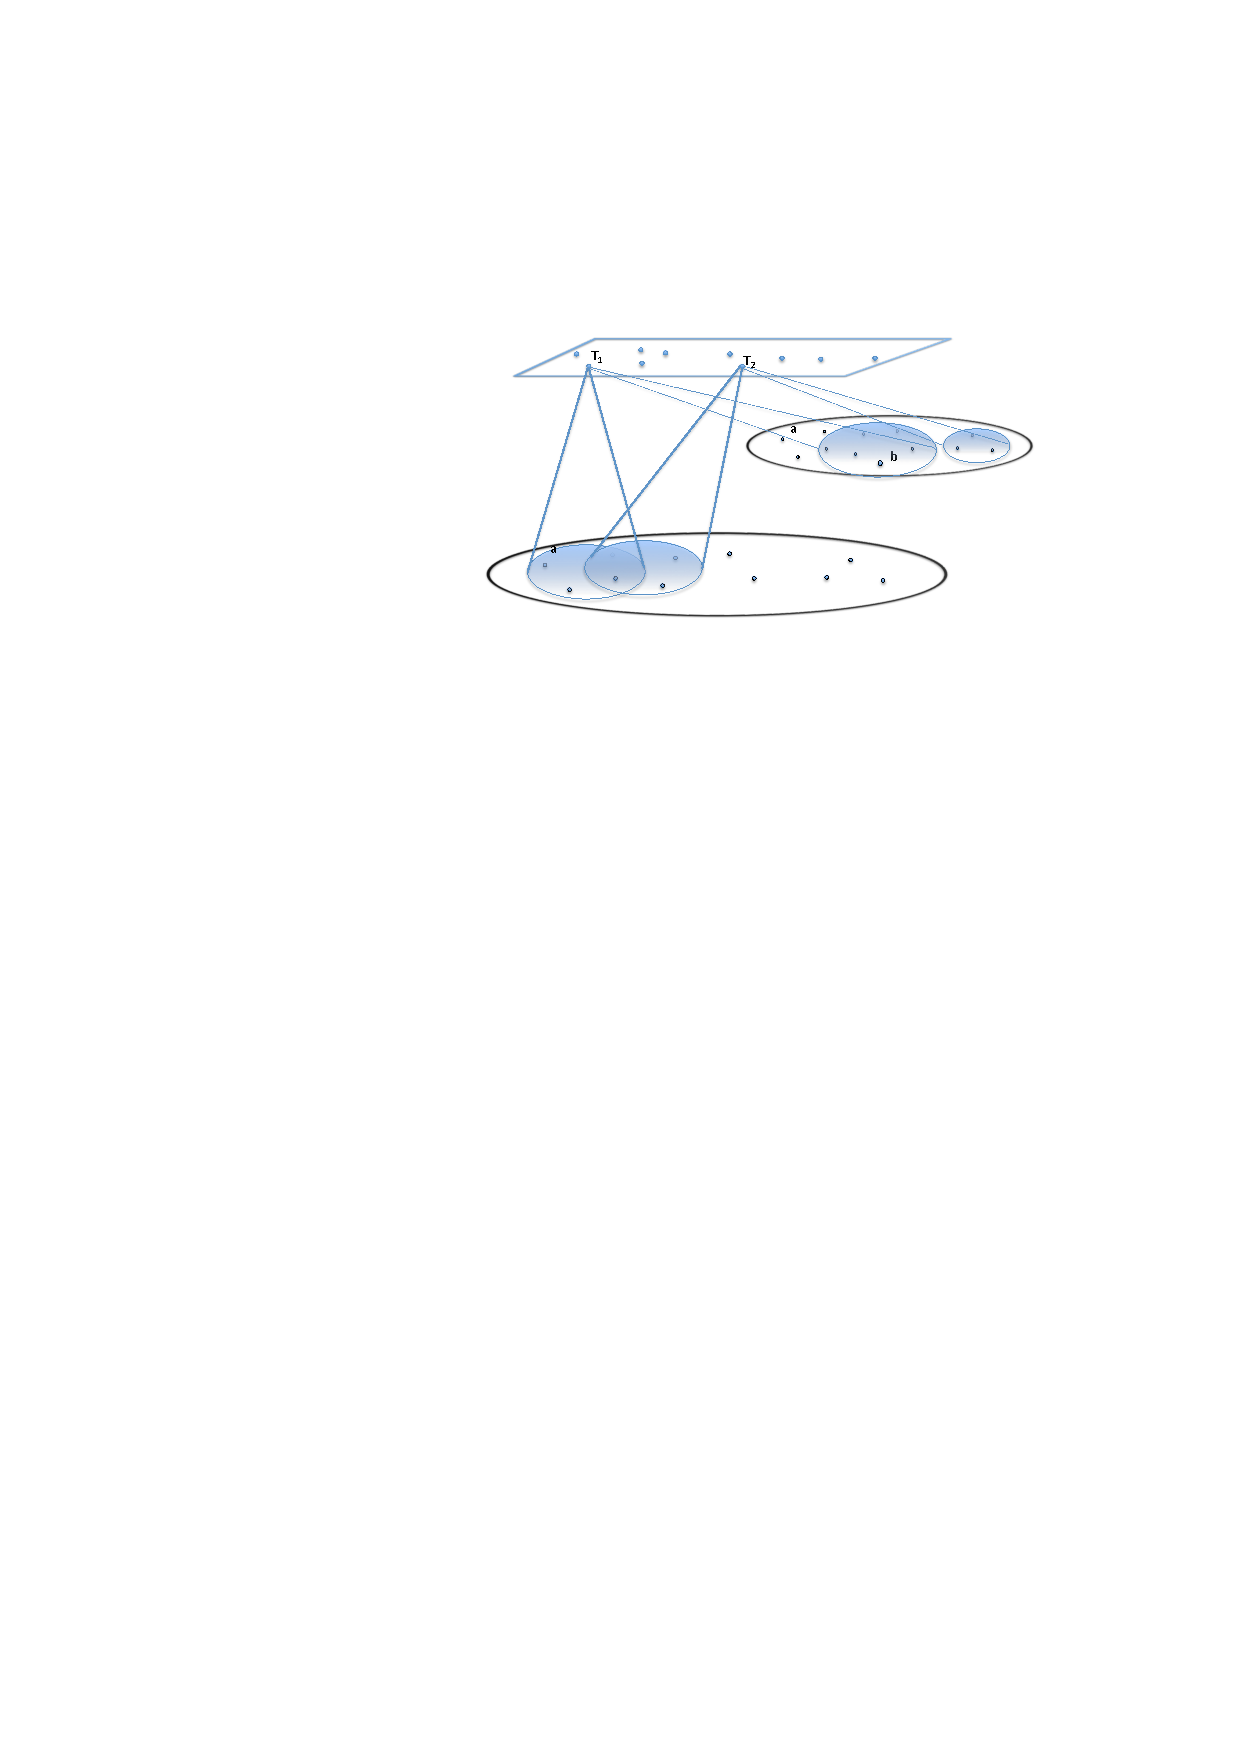
\includegraphics[width=\textwidth]{modal}
\begin{adjustbox}{max width=\textwidth}
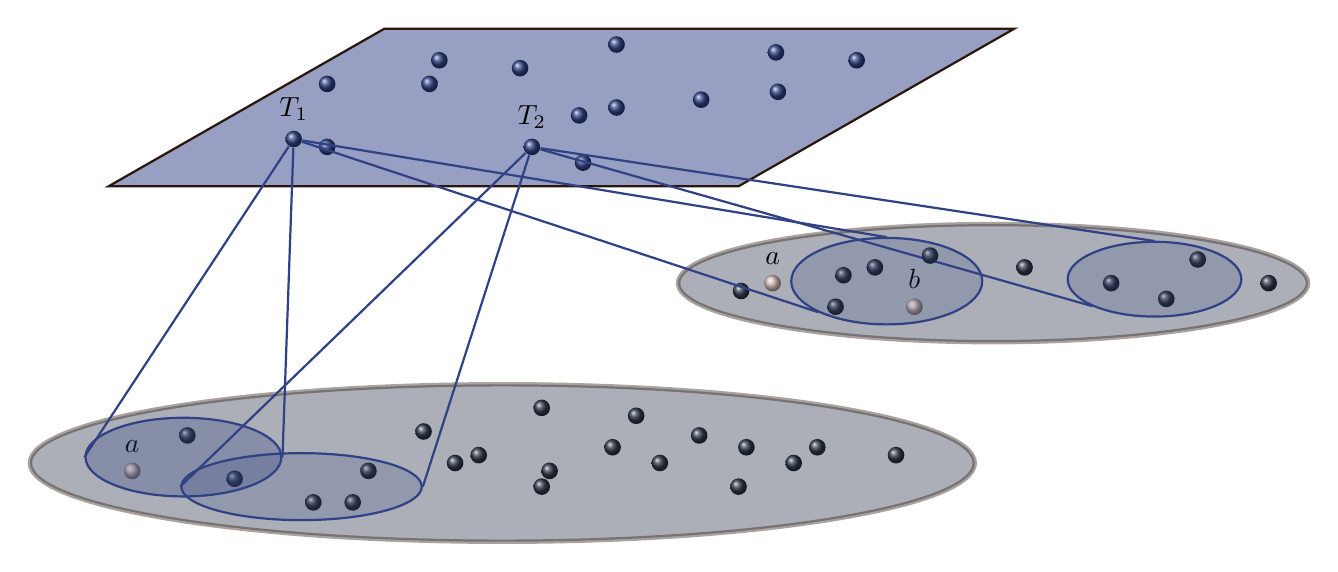
\begin{tikzpicture}[
  type/.style={circle, inner sep=0pt, minimum size=6pt, ball color=BTypeCol},
  firsttype/.style={circle, inner sep=0pt, minimum size=6pt, ball color=FirstTypeCol},
  secondtype/.style={circle, inner sep=0pt, minimum size=6pt, ball color=SecondTypeCol},
  objects/.style={circle, inner sep=0pt, minimum size=6pt, ball color=ObjectCol},
  modalobjects/.style={circle, inner sep=0pt, minimum size=6pt, ball color=ModalCol}
  ]

  % basic types:
  \begin{scope}[
    % every node/.append style={yslant=0,xslant=1.75},
    yslant=0,xslant=1.75
    ]
    \filldraw [fill=BTypeCol, draw=BorderCol, thick, fill opacity=0.5] (0,0) rectangle (8,2);

    \foreach \x/\y in {0.5/1.3, 1.4/1.6, 1.8/1.3, 1.9/0.5, 3.3/1.8, 2.6/1.5, 4.4/0.9, 4.7/1, 5.5/0.3, 5.6/1.1, 5.5/1.7, 6.4/1.2, 6.7/1.6} {
      \node [type] at (\x,\y) {};
    }

    \node [coordinate] (btypeleft) at (0,1) {};
    \node [coordinate] (btyperight) at (8,1) {};

    \node [type, label=above:$T_1$] (t1) at (1.3,0.6) {};
    \node [type, label=above:$T_2$] (t2) at (4.5,0.5) {};
  \end{scope}    


  % objects:
  \begin{scope}[
    % every node/.append style={yslant=0,xslant=1.75},
    %yslant=0,xslant=1.75,
    yshift=-100
    ]
    \filldraw [fill=ObjectCol, opacity=0.4, draw=BorderCol, ultra thick] (5,0) ellipse (6 and 1);

    \foreach \a/\b in {5.5/0.7, 6.4/0.2, 6.7/0.6, 7/0, 7.5/0.35, 8/-0.3, 8.1/0.2, 8.7/0, 9/0.2, 10/0.1} {
      \node [objects] at (\a,\b) {};
    }
    % for T1 from BType:
    \node [modalobjects, label=above:$a$] (o1) at (0.3,-0.1) {}; 
    \node [objects] (o2) at (1,0.35) {}; 
    \node [objects] (o3) at (1.6,-0.2) {};
    \node [ellipse, fit=(o1) (o2) (o3), yscale=0.7, draw=BTypeCol, thick, fill=BTypeCol, fill opacity=0.3] (fitA) {};
    \draw [BTypeCol, thick] (t1) -- (fitA.east);
    \draw [BTypeCol, thick] (t1) -- (fitA.west);

    % for T2 from BType:
    \node [objects] (o4) at (2.6,-0.5) {};
    \node [objects] (o5) at (3.1,-0.5) {};
    \node [objects] (o6) at (3.3,-0.1) {};
    \node [ellipse, fit=(o3) (o4) (o5) (o6), yscale=0.7, draw=BTypeCol, thick, fill=BTypeCol, fill opacity=0.2] (fitB) {};
    \draw [BTypeCol, thick] (t2) -- (fitB.east);
    \draw [BTypeCol, thick] (t2) -- (fitB.west);

    % % for T2 from Type1:
     \node [objects] (o7) at (4,0.4) {};
     \node [objects] (o8) at (4.4,0) {}; 
     \node [objects] (o9) at (4.7,0.1) {};
    % \node [ellipse, fit=(o3) (o4) (o5) (o6) (o7) (o8) (o9), yscale=0.6, xscale=0.9, draw=FirstTypeCol, thick, fill=FirstTypeCol, fill opacity=0.2] (fitC) {};

    % % for T2 from Type2:
     \node [objects] (o10) at (5.5,-0.3) {};
     \node [objects] (o11) at (5.6,-0.1) {};
    % \node [ellipse, fit=(o3) (o4) (o5) (o6) (o7) (o8) (o9) (o10) (o11), yscale=0.7, xscale=0.8, draw=SecondTypeCol, thick, fill=SecondTypeCol, fill opacity=0.2] (fitD) {};
  \end{scope}


  % modal types:
  \begin{scope}[
    % every node/.append style={yslant=0,xslant=1.75},
    %yslant=0,xslant=1.75,
    yshift=-35, 
    xshift=220
    ]
    \filldraw [fill=ObjectCol, opacity=0.4, draw=BorderCol, ultra thick] (3.5,0) ellipse (4 and 0.75);

    \foreach \a/\b in {0.3/-0.1, 1.5/-0.3, 3.9/0.2, 7/0} {
      \node [objects] at (\a,\b) {};
    }
    \node [modalobjects, label=above:$a$] at (0.7,0) {};
    \node [objects] (i1) at (5.7,-0.2) {};
    \node [objects] (i2) at (6.1,0.3) {};
    \node [objects] (i3) at (5,0) {};
    \node [ellipse, fit=(i1) (i2) (i3), yscale=0.7, draw=BTypeCol,
    thick, fill=BTypeCol, fill opacity=0.2] (fitAA) {};
    \draw [BTypeCol, thick] (t2) -- (fitAA.north);
    \draw [BTypeCol, thick] (t2) -- (fitAA.south west);

    \node [objects] (i4) at (1.6,0.1) {};
    \node [objects] (i5) at (2,0.2) {};
    \node [modalobjects, label=above:$b$] (i6) at (2.5,-0.3) {};
    \node [objects] (i7) at (2.7,0.35) {};
    \node [ellipse, fit=(i4) (i5) (i6) (i7), yscale=0.7, xscale=1.1,
    draw=BTypeCol, thick, fill=BTypeCol, fill opacity=0.2] (fitBB) {};
    \draw [BTypeCol, thick] (t1) -- (fitBB.north);
    \draw [BTypeCol, thick] (t1) -- (fitBB.south west);
  \end{scope}


  % % Type1:
  % \begin{scope}[
  %   % every node/.append style={yslant=0,xslant=1.75},
  %   yslant=0,xslant=1.75,
  %   xshift=-100,
  %   yshift=80
  %   ]
  %   \filldraw [fill=FirstTypeCol, draw=BorderCol, thick, fill opacity=0.3] (0,0) rectangle (8,2);
  %   \node [coordinate] (firsttypeleft) at (0,1) {};
  %   \node [coordinate] (firsttyperight) at (8,1) {};

  %   \foreach \x/\y in {0.45/1.4, 1.4/1.6, 1.9/0.5, 3.3/1.8, 2.6/1.5, 4.7/1, 5.5/0.3, 5.6/1.1,  6.7/1.6} {
  %     \node [firsttype] at (\x,\y) {};
  %   }

  %   \node [firsttype, label=above:$T_1$] (ft1) at (1.8,1.1) {};
  %   \node [firsttype, label=above:$T_2$] (ft2) at (5.8,0.7) {};
  %   \node [firsttype, label=above:$T_3$] (ft3) at (6.4,1.2) {};
  %   \node [firsttype, label=above:{\textbf{Type$^1$}}] (ft) at (4,0.4) {};

  %   \draw [FirstTypeCol, thick] (ft) -- (btypeleft);
  %   \draw [FirstTypeCol, thick] (ft) -- (btyperight);
    
  %   \draw [FirstTypeCol, thick] (ft2) -- (fitC.east);
  %   \draw [FirstTypeCol, thick] (ft2) -- (fitC.west);
  % \end{scope}    


  % % Type2:
  % \begin{scope}[
  %   % every node/.append style={yslant=0,xslant=1.75},
  %   yslant=0,xslant=1.75,
  %   xshift=-200,
  %   yshift=160
  %   ]
  %   \filldraw [fill=SecondTypeCol, draw=BorderCol, thick, fill opacity=0.1] (0,0) rectangle (8,2);
  %   \foreach \x/\y in {1.4/1.6, 1.9/0.5, 3.2/1.5, 4.7/1, 5.4/1.2, 5.8/0.3, 6/0.3,  6.2/1.6} {
  %     \node [secondtype] at (\x,\y) {};
  %   }

  %   \node [secondtype, label=above:$T_1$] (st1) at (1.2,1) {};
  %   \node [secondtype, label=above:$T_2$] (st2) at (4.8,0.7) {};
  %   \node [secondtype, label=above:$T_3$] (st3) at (2.6,1.3) {};
  %   \node [secondtype, label=above:{\textbf{Type$^2$}}] (st) at (3.4,0.5) {};

  %   \draw [SecondTypeCol, thick] (st) -- (firsttypeleft);
  %   \draw [SecondTypeCol, thick] (st) -- (firsttyperight);
    
  %   \draw [SecondTypeCol, thick] (st2) -- (fitD.east);
  %   \draw [SecondTypeCol, thick] (st2) -- (fitD.west);
  % \end{scope}    
\end{tikzpicture}
\end{adjustbox}

\caption{Modal system of basic types}
\label{fig:modal}
\end{figure}
The object $a$ is
of type $T_1$ in the first possibility but not in the second
possibility.  There is an object, $b$, of type $T_1$ in the second
possibility.  $b$ does not exist at all in the first possibility.
In the
figure we just show two possibilities but our general definition in Appendix~\ref{sec:basic}
allows for there to be any number of possibilities, including
infinitely many.

Given this apparatus we define four simple modal notions:
\begin{description}

\item[(necessary) equivalence] Two types are (necessarily) equivalent
  just in case the extension of one type is identical with that of
  the other type in all the possibilities.  While the different
  possibilities may provide different extensions for the types, it
  will always be the case that in any given possibility the two types
  will have the same extension.

\item[subtype] One type is a subtype of another just in case whatever
  possibility you look at it is always the case that the extension of
  the first type is a subset of the extension of the second.  We can
  also say that the first type ``entails'' the second, that is, any
  object which is of the first type will also be of the second type,
  no matter which possibility you are considering.

\item[necessity] The notion of necessity we characterize for a type
  could be glossed as ``necessarily realized'' or ``necessarily
  instantiated''.  A type will be necessary just in case there is
  something of the type in all the possibilities.

\item[possibility] This notion corresponds to ``possibly realized'' or
  ``possibly instantiated''.  A type will be possible just in case
  there is some possibility according to which it has a non-null
  extension.

\end{description}
These notions are made precise in Appendix~\ref{sec:basic}.  Note that
all of these notions are relativized to the modal system you are
considering and the possibilities it offers.  We may think of the
family of assignments $\mathcal{A}$ as providing a modal base
(cf. Kratzer) or alternatives (in the sense of ????).  For these kinds
of applications we may wish to consider very small families of
assignments corresponding to the knowledge we have.  Alternatively, we
may want to consider strong logical variants of these modal notions
where we consider all the logical possibilities, for example, all
possible assignments of extensions to types.

So far we have talked about modal systems of basic types.  Modal
systems of complex types, where we introduce ptypes, create a
minor complication.  What ptypes that are present in a system depends
on what objects there are of the types that are used in the arities of
the predicates.  Thus if we have some predicate $r$ with arity
$\langle\textit{Ind},\textit{Ind}\rangle$ and a possibility where the
set assigned to \textit{Ind} is $\{a,b\}$ then according to that
possibility the ptypes formed with $r$ will be $r(a,a)$, $r(a,b)$,
$r(b,a)$ and $r(b,b)$.  In a possibility where \textit{Ind} is
assigned a different set the set of available ptypes will be
different.  It is an important feature of type theories with types
constructed from predicates that the collection of such types depends
on what objects are available as arguments to the predicates.  This
makes type theory very different from a logical language such as
predicate calculus where the notion of well-formedness of syntactic
expressions containing predicates is defined independently of what is
provided by the model as denotations of arguments to the predicate.

This leads us (in Appendix~\ref{app:modal}) to define two variants of
each of our modal notions: \textit{restrictive} variants which are only defined
for types which exist in all possibilities and \textit{inclusive}
variants which require that the modal definition holds for all the
possibilities in which the types exist and disregards those in which
the types do not exist.  For example, a type is \textit{necessary}$_r$
(that is, ``restrictively necessary'') just in case the type is
available in all possibilities and has a non-empty set of witnesses in
all possibilities.  It is \textit{necessary}$_i$ (``inclusively
necessary'') just in case in all the possibilities in which the type
is provided it has a non-empty set of witnesses.  It is clear that if
a type is necessary$_r$ it will also be necessary$_i$ but there may be
types which are necessary$_i$ but not necessary$_r$ (if the type is
not provided in all possibilities).  A similar relationship between
the restrictive and inclusive notions holds for all the modal notions
we have discussed.

There may be significant classes of modal type systems in which the
types available in the different possibilities do not vary.  This
could be achieved by requiring that the types used in the arities of
predicates always have the same witnesses in all the possibilities.
This seems feasible if we restrict the types used in predicate arities
to basic ontological categories such as individual or time point.  It
seems reasonable to consider modal systems in which an individual in
one possibility will be an individual in any other possibility, for
example.  It seems reasonable to say that we wish to consider
possibilities where, for example, Kim is a man rather than a woman,
but not possibilities where Kim is a point in time rather than an
individual.  However, the notion ``basic ontological category'' is a
slippery one and we do not want to be forced to make commitments about that.

In the definition of a system of complex types in
section~\ref{app:comptypes}  we call the pair of an assignment to
basic types and assignment to ptypes, $\langle A,F\rangle$, a \textit{model} because of its
similarity to first order models.\footnote{For a more detailed
  discussion of the relationship between this and first order models
  as used in the interpretation of first order logic see
  \cite{Cooperforthcoming}.} The model provides an interface
between 
the type theoretical system and a domain external to the type theory.
The natural domain to relate to the type theory is that of individuals
and situations, that is the kind of things we can perceive or at least
consider as possibilities.  However, we may want to use models which
relate to our perceptual apparatus, as in \cite{Larsson2011}, rather
than directly to the world.  This can also be the key for relating the
type theory to a dynamically changing world where the models
representing our perceived possibilities are not fixed.  % We will
% return to this in Chapter~\ref{ch:coord}.



\section{Intensionality: propositions as types}

Kim continues to think about the boy and the dog as she walks along.
It was fun to see them playing together.  They seemed so happy.  The
boy obviously thought that the dog was a good playmate.  Kim is not
only able to perceive events as being of certain types.  She is able
to recall and reflect on these types.  She is able to form attitudes
towards these types: it was fun that the boy and the dog were playing but
a little worrying that they were so close to the pond.  This means
that the types themselves seem to be arguments to predicates like
`fun' and `worrying'.  This seems to be an important human ability --
not only to be able to take part in or observe an event and find it
fun or worrying but to be able to reflect independently of the actual
occurrence of the event that it or in general similar events are fun
or worrying.  This is a source of great richness in human cognition in
that it enables us to consider situation types independently of their
actual instantiation.\footnote{This richness also has its downside in
  that we often become so engaged in our internal cognitive abstraction
  that it can be difficult to be fully present and conscious of our
  direct perception of the world -- for example, worrying about what
  might happen in the future rather than enjoying the present.}  This
abstraction also enables us to consider what attitudes other
individuals might have.  For example, Kim believes that the boy
thought that the dog was a good playmate.  She is able to ascribe this
belief to the boy.  Furthermore, we are able to reflect on Kim's state
of mind where she has a belief concerning the type of situation where
the boy thinks that the dog was a good playmate.  And somebody else
could consider of us that we have a certain belief about Kim
concerning her belief about the boy's belief.  There
is in principle no limit to the depth of recursion concerning our
attitudes towards types.

We propose to capture this reflective nature of human cognition by
making the type theory technically \textit{reflective} in the sense
that we
allow types themselves to be objects which can belong to other types.
In classical model theoretic semantics we think of
\textit{believe} as corresponding to a relation between individuals
and propositions.  In our type theory, however, we are subscribing to
the ``propositions as types'' view which comes to us via
\cite{Martin-Loef1984} but has its origins in intuitionistic logic
[????].  Propositions are true or false.  Types of situations such as
hug($a$,$b$) correspond to propositions in the sense that if they are
non-empty then the proposition is true. If there is nothing of this
type then it is false.  The reasoning is thus that we do not need
propositions in our system as separate semantic objects if we already
have types.  We can use the types to play the role of propositions.
To believe a type is to believe it to be non-empty.  From the point of view
of a type theory for cognition in which we connect types to our basic
perceptual ability, this provides a welcome link between our perceptual
ability and our ability to entertain propositions (that is,  to
consider whether they are
true or false).

A predicate like `believe' which represents that an individual has an
attitude (of belief) to a certain type should thus have an arity which
requires its arguments to be an individual and a type.  That is, we
should be able to construct the type believe($c$, hug($a$,$b$))
corresponding to \textit{$c$ believes that $a$ hugs $b$}.  We thus
create \textit{intensional} type systems where types themselves can be treated
as objects and belong to types.  Care has to be taken in constructing
such systems in order to avoid paradoxes.  We use a standard
technique known as stratification \cite{Turner2005}.  We start with a
basic type system and then add higher order levels of types.  Each
higher order includes the types of the order immediately below as
objects.  In each of these higher orders $n$ there will be a type of
all types of the order $n-1$ but there is no ultimate ``type of all
types'' -- such a type would have to have itself as an object.  This
is made precise in Appendix~\ref{app:int}.  For more detailed
discussion see \cite{Cooperforthcoming}.  
Figure~\ref{fig:intensionalmodal} represents an intensional modal type
system where we indicate just the initial
three orders of an infinite hierarchy of type orders.
\begin{figure}[h]
%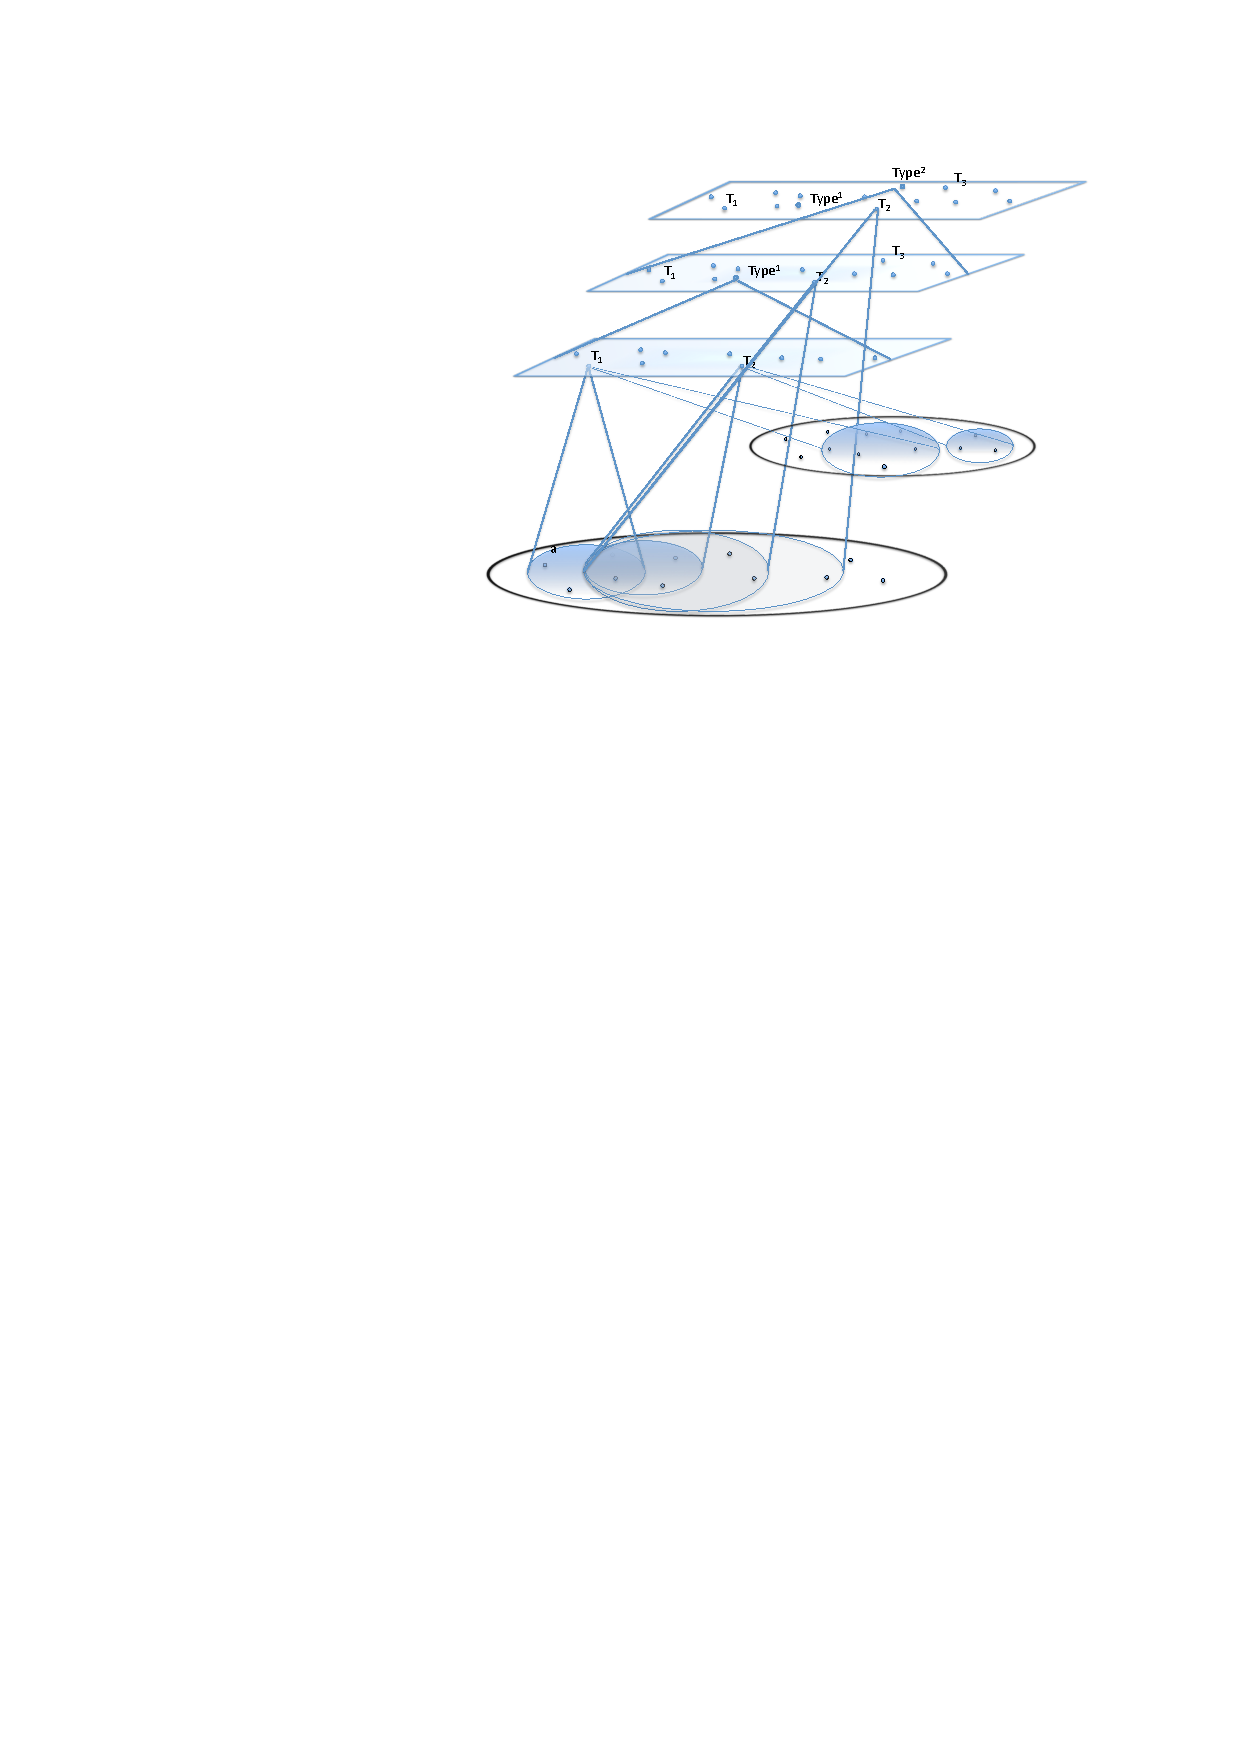
\includegraphics[width=\textwidth]{intensionalmodal}
\begin{adjustbox}{max width=\textwidth}
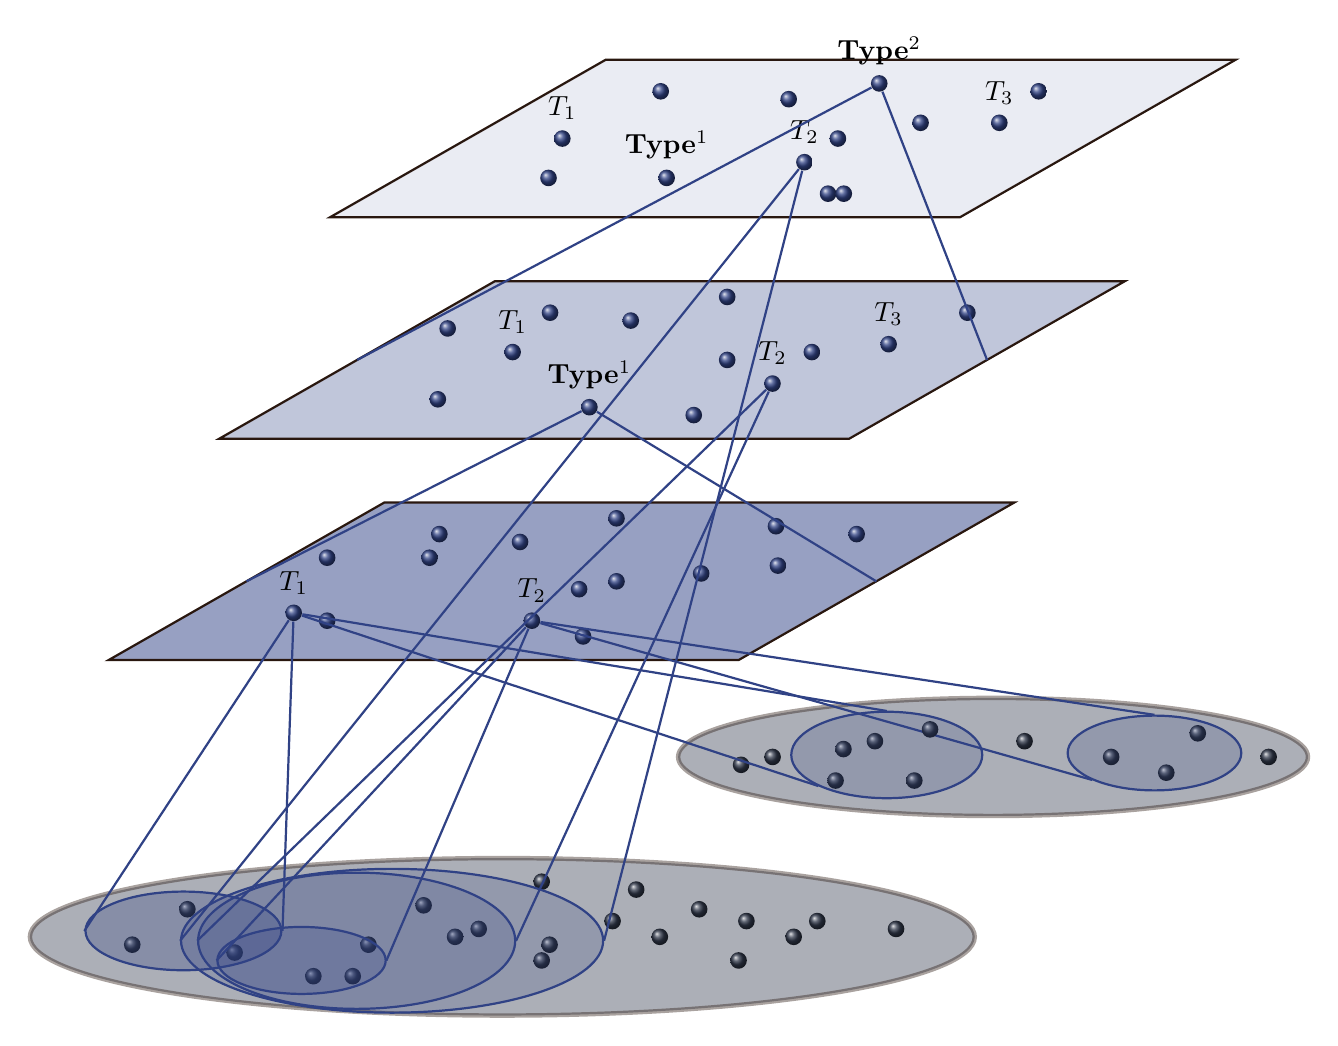
\begin{tikzpicture}[
  type/.style={circle, inner sep=0pt, minimum size=6pt, ball color=BTypeCol},
  firsttype/.style={circle, inner sep=0pt, minimum size=6pt, ball color=FirstTypeCol},
  secondtype/.style={circle, inner sep=0pt, minimum size=6pt, ball color=SecondTypeCol},
  objects/.style={circle, inner sep=0pt, minimum size=6pt, ball color=ObjectCol},
  modalobjects/.style={circle, inner sep=0pt, minimum size=6pt, ball color=ModalCol}
  ]

  % basic types:
  \begin{scope}[
    % every node/.append style={yslant=0,xslant=1.75},
    yslant=0,xslant=1.75
    ]
    \filldraw [fill=BTypeCol, draw=BorderCol, thick, fill opacity=0.5] (0,0) rectangle (8,2);

    \foreach \x/\y in {0.5/1.3, 1.4/1.6, 1.8/1.3, 1.9/0.5, 3.3/1.8, 2.6/1.5, 4.4/0.9, 4.7/1, 5.5/0.3, 5.6/1.1, 5.5/1.7, 6.4/1.2, 6.7/1.6} {
      \node [type] at (\x,\y) {};
    }

    \node [coordinate] (btypeleft) at (0,1) {};
    \node [coordinate] (btyperight) at (8,1) {};

    \node [type, label=above:$T_1$] (t1) at (1.3,0.6) {};
    \node [type, label=above:$T_2$] (t2) at (4.5,0.5) {};
  \end{scope}    


  % objects:
  \begin{scope}[
    % every node/.append style={yslant=0,xslant=1.75},
    %yslant=0,xslant=1.75,
    yshift=-100
    ]
    \filldraw [fill=ObjectCol, opacity=0.4, draw=BorderCol, ultra thick] (5,0) ellipse (6 and 1);

    \foreach \a/\b in {5.5/0.7, 6.4/0.2, 6.7/0.6, 7/0, 7.5/0.35, 8/-0.3, 8.1/0.2, 8.7/0, 9/0.2, 10/0.1} {
      \node [objects] at (\a,\b) {};
    }
    % for T1 from BType:
    \node [objects] (o1) at (0.3,-0.1) {}; 
    \node [objects] (o2) at (1,0.35) {}; 
    \node [objects] (o3) at (1.6,-0.2) {};
    \node [ellipse, fit=(o1) (o2) (o3), yscale=0.7, draw=BTypeCol, thick, fill=BTypeCol, fill opacity=0.3] (fitA) {};
    \draw [BTypeCol, thick] (t1) -- (fitA.east);
    \draw [BTypeCol, thick] (t1) -- (fitA.west);

    % for T2 from BType:
    \node [objects] (o4) at (2.6,-0.5) {};
    \node [objects] (o5) at (3.1,-0.5) {};
    \node [objects] (o6) at (3.3,-0.1) {};
    \node [ellipse, fit=(o3) (o4) (o5) (o6), yscale=0.7, xscale=0.7, draw=BTypeCol, thick, fill=BTypeCol, fill opacity=0.2] (fitB) {};
    \draw [BTypeCol, thick] (t2) -- (fitB.east);
    \draw [BTypeCol, thick] (t2) -- (fitB.west);

    % for T2 from Type1:
    \node [objects] (o7) at (4,0.4) {};
    \node [objects] (o8) at (4.4,0) {}; 
    \node [objects] (o9) at (4.7,0.1) {};
    \node [ellipse, fit=(o3) (o4) (o5) (o6) (o7) (o8) (o9), yscale=0.9, xscale=0.8, draw=FirstTypeCol, thick, fill=FirstTypeCol, fill opacity=0.2] (fitC) {};

    % for T2 from Type2:
    \node [objects] (o10) at (5.5,-0.3) {};
    \node [objects] (o11) at (5.6,-0.1) {};
    \node [ellipse, fit=(o3) (o4) (o5) (o6) (o7) (o8) (o9) (o10) (o11), yscale=0.95, xscale=0.85, draw=SecondTypeCol, thick, fill=SecondTypeCol, fill opacity=0.2] (fitD) {};
  \end{scope}


  % modal types:
  \begin{scope}[
    % every node/.append style={yslant=0,xslant=1.75},
    %yslant=0,xslant=1.75,
    yshift=-35, 
    xshift=220
    ]
    \filldraw [fill=ObjectCol, opacity=0.4, draw=BorderCol, ultra thick] (3.5,0) ellipse (4 and 0.75);

    \foreach \a/\b in {0.3/-0.1, 1.5/-0.3, 3.9/0.2, 7/0} {
      \node [objects] at (\a,\b) {};
    }
    \node [objects] at (0.7,0) {};
    \node [objects] (i1) at (5.7,-0.2) {};
    \node [objects] (i2) at (6.1,0.3) {};
    \node [objects] (i3) at (5,0) {};
    \node [ellipse, fit=(i1) (i2) (i3), yscale=0.7, draw=BTypeCol,
    thick, fill=BTypeCol, fill opacity=0.2] (fitAA) {};
\draw [BTypeCol, thick] (t2) -- (fitAA.north);
    \draw [BTypeCol, thick] (t2) -- (fitAA.south west);

    \node [objects] (i4) at (1.6,0.1) {};
    \node [objects] (i5) at (2,0.2) {};
    \node [objects] (i6) at (2.5,-0.3) {};
    \node [objects] (i7) at (2.7,0.35) {};
    \node [ellipse, fit=(i4) (i5) (i6) (i7), yscale=0.7, xscale=1.1,
    draw=BTypeCol, thick, fill=BTypeCol, fill opacity=0.2] (fitBB) {};
    \draw [BTypeCol, thick] (t1) -- (fitBB.north);
    \draw [BTypeCol, thick] (t1) -- (fitBB.south west);
  \end{scope}


  % Type1:
  \begin{scope}[
    % every node/.append style={yslant=0,xslant=1.75},
    yslant=0,xslant=1.75,
    xshift=-100,
    yshift=80
    ]
    \filldraw [fill=FirstTypeCol, draw=BorderCol, thick, fill opacity=0.3] (0,0) rectangle (8,2);
    \node [coordinate] (firsttypeleft) at (0,1) {};
    \node [coordinate] (firsttyperight) at (8,1) {};

    \foreach \x/\y in {0.45/1.4, 1.4/1.6, 1.9/0.5, 3.3/1.8, 2.6/1.5, 4.7/1, 5.5/0.3, 5.6/1.1,  6.7/1.6} {
      \node [firsttype] at (\x,\y) {};
    }

    \node [firsttype, label=above:$T_1$] (ft1) at (1.8,1.1) {};
    \node [firsttype, label=above:$T_2$] (ft2) at (5.8,0.7) {};
    \node [firsttype, label=above:$T_3$] (ft3) at (6.4,1.2) {};
    \node [firsttype, label=above:{\textbf{Type$^1$}}] (ft) at (4,0.4) {};

    \draw [FirstTypeCol, thick] (ft) -- (btypeleft);
    \draw [FirstTypeCol, thick] (ft) -- (btyperight);
    
    \draw [FirstTypeCol, thick] (ft2) -- (fitC.east);
    \draw [FirstTypeCol, thick] (ft2) -- (fitC.west);
  \end{scope}    


  % Type2:
  \begin{scope}[
    % every node/.append style={yslant=0,xslant=1.75},
    yslant=0,xslant=1.75,
    xshift=-200,
    yshift=160
    ]
    \filldraw [fill=SecondTypeCol, draw=BorderCol, thick, fill opacity=0.1] (0,0) rectangle (8,2);
    \foreach \x/\y in {1.4/1.6, 1.9/0.5, 3.2/1.5, 4.7/1, 5.4/1.2, 5.8/0.3, 6/0.3,  6.2/1.6} {
      \node [secondtype] at (\x,\y) {};
    }

    \node [secondtype, label=above:$T_1$] (st1) at (1.2,1) {};
    \node [secondtype, label=above:$T_2$] (st2) at (4.8,0.7) {};
    \node [secondtype, label=above:$T_3$] (st3) at (6.4,1.2) {};
    \node [secondtype, label=above:{\textbf{Type$^1$}}] (st4) at
    (3.4,0.5) {};
    \node [secondtype, label=above:{\textbf{Type$^2$}}] (st) at
    (4.0,1.7) {};

    \draw [SecondTypeCol, thick] (st) -- (firsttypeleft);
    \draw [SecondTypeCol, thick] (st) -- (firsttyperight);
    
    \draw [SecondTypeCol, thick] (st2) -- (fitD.east);
    \draw [SecondTypeCol, thick] (st2) -- (fitD.west);
  \end{scope}    
\end{tikzpicture}
\end{adjustbox}

\caption{Intensional modal type system}
\label{fig:intensionalmodal}
\end{figure}

\section{Summary}


%%% Local Variables: 
%%% mode: latex
%%% TeX-master: "ttl"
%%% End: 




% \chapter{Information exchange}
% \chapter{Information states and information exchange}
% \label{ch:infex}

\chapter[From event perception and action to information states and
information exchange][Information states and information
exchange]{From event perception and action to information states and information exchange}
\label{ch:infex}
\setcounter{equation}{0}

\section{Introduction}
In Chapter~\ref{ch:percint} we talked about two kinds of situation
types: ptypes and record types.  This presents a static view of
situations which are events, that is, those situations in which a
change takes place.  In Section~\ref{sec:ev-strings} we will introduce
string types which enable us to treat events as strings of smaller events.

\section{The string theory of events}
\label{sec:ev-strings}

Kim stands and watches the boy and the dog for a while.  They start to
play fetch.\footnote{\url{http://en.wikipedia.org/wiki/Fetch_(game)},
  accessed 10th Oct 2011.}  This is a moderately complex game in that
it consists of a number of components which are carried out in a
certain order.  The boy picks up a stick attracts the attention of
the dog (possibly shouting ``Fetch!''), and throws the stick.  The dog
runs after the stick, picks it up in his mouth and brings it back to
the boy.  This sequence can be repeated arbitrarily many times.  One
thing that becomes clear from this is that events do not happen in a
single moment but rather they are stretched out over intervals of
time, characterized by the sub-events that constitute them.  So if we were to have a type of event (that is, a type of situation)
play\_fetch($a$,$b$,$c$) where $a$ is a human, $b$ is a dog and
$c$ is a stick % , then $t$ should not be a moment of time but a time
% \textit{interval} starting with the time of the beginning of the event
% and ending with the time of the end of the event.  But 
we can %could also
say something about the series of subevents that we have identified.
So we might draw an informal diagram something like
Figure~\ref{fig:fetch}.
\begin{figure} 

%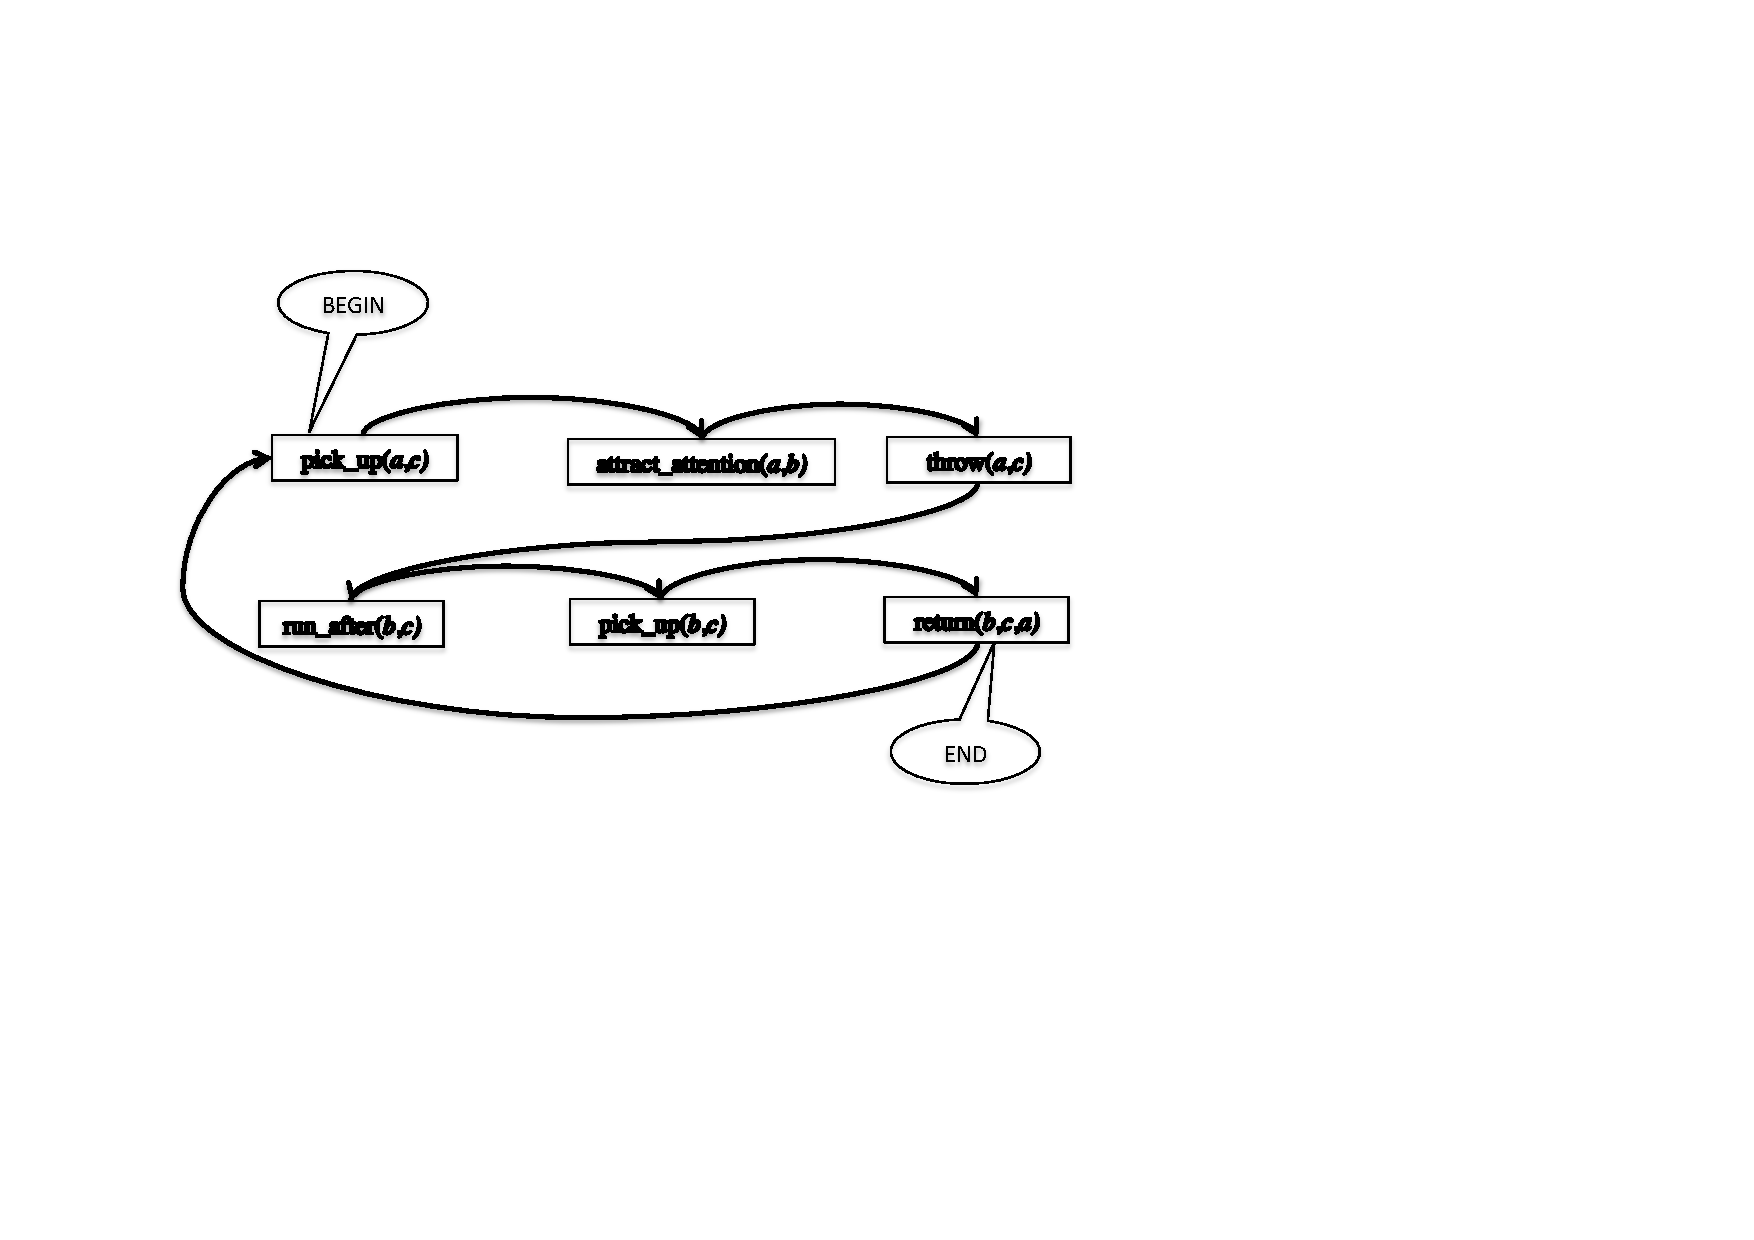
\includegraphics[width=6in]{fetch}

\hspace*{-4em}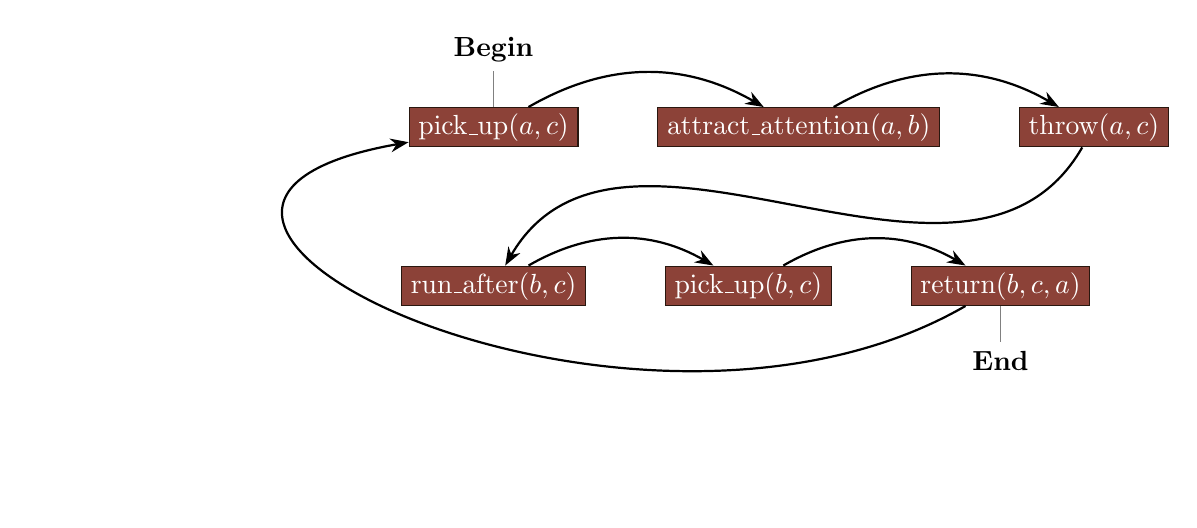
\begin{tikzpicture}[
  play/.style={rectangle, fill=Lamentation5, draw=Lamentation1, text=white, text depth=0.25ex, text height=1.5ex}
  ]

\node [play, pin=above:\textbf{Begin}] (p1) {pick\_up($a,c$)};
\node [play, right=of p1] (p2) {attract\_attention($a,b$)};
\node [play, right=of p2] (p3) {throw($a,c$)};
\node [play, below=1.5 of p1] (p4) {run\_after($b,c$)};
\node [play, right=of p4] (p5) {pick\_up($b,c$)};
\node [play, right=of p5, pin=below:\textbf{End}] (p6) {return($b,c,a$)};

\path [-{Stealth[]}, thick] 
(p1) edge [bend left] (p2)
(p2) edge [bend left] (p3)
(p3) edge [out=240, in=60] (p4)
(p4) edge [bend left] (p5)
(p5) edge [bend left] (p6)
(p6) edge [out=210, in=190, looseness=1.7] (p1);  
\end{tikzpicture}


\caption{play\_fetch($a$,$b$,$c$)}
\label{fig:fetch}
\end{figure}




   

In an important series of papers including
\cite{Fernando2004,Fernando2006,Fernando2008,Fernando2009,Fernando2011,Fernando2015}, Fernando introduces a finite state
approach to event analysis where events are analyzed in terms of
finite state automata something like what we have represented in
Figure~\ref{fig:fetch-fs}.
\begin{figure} 

%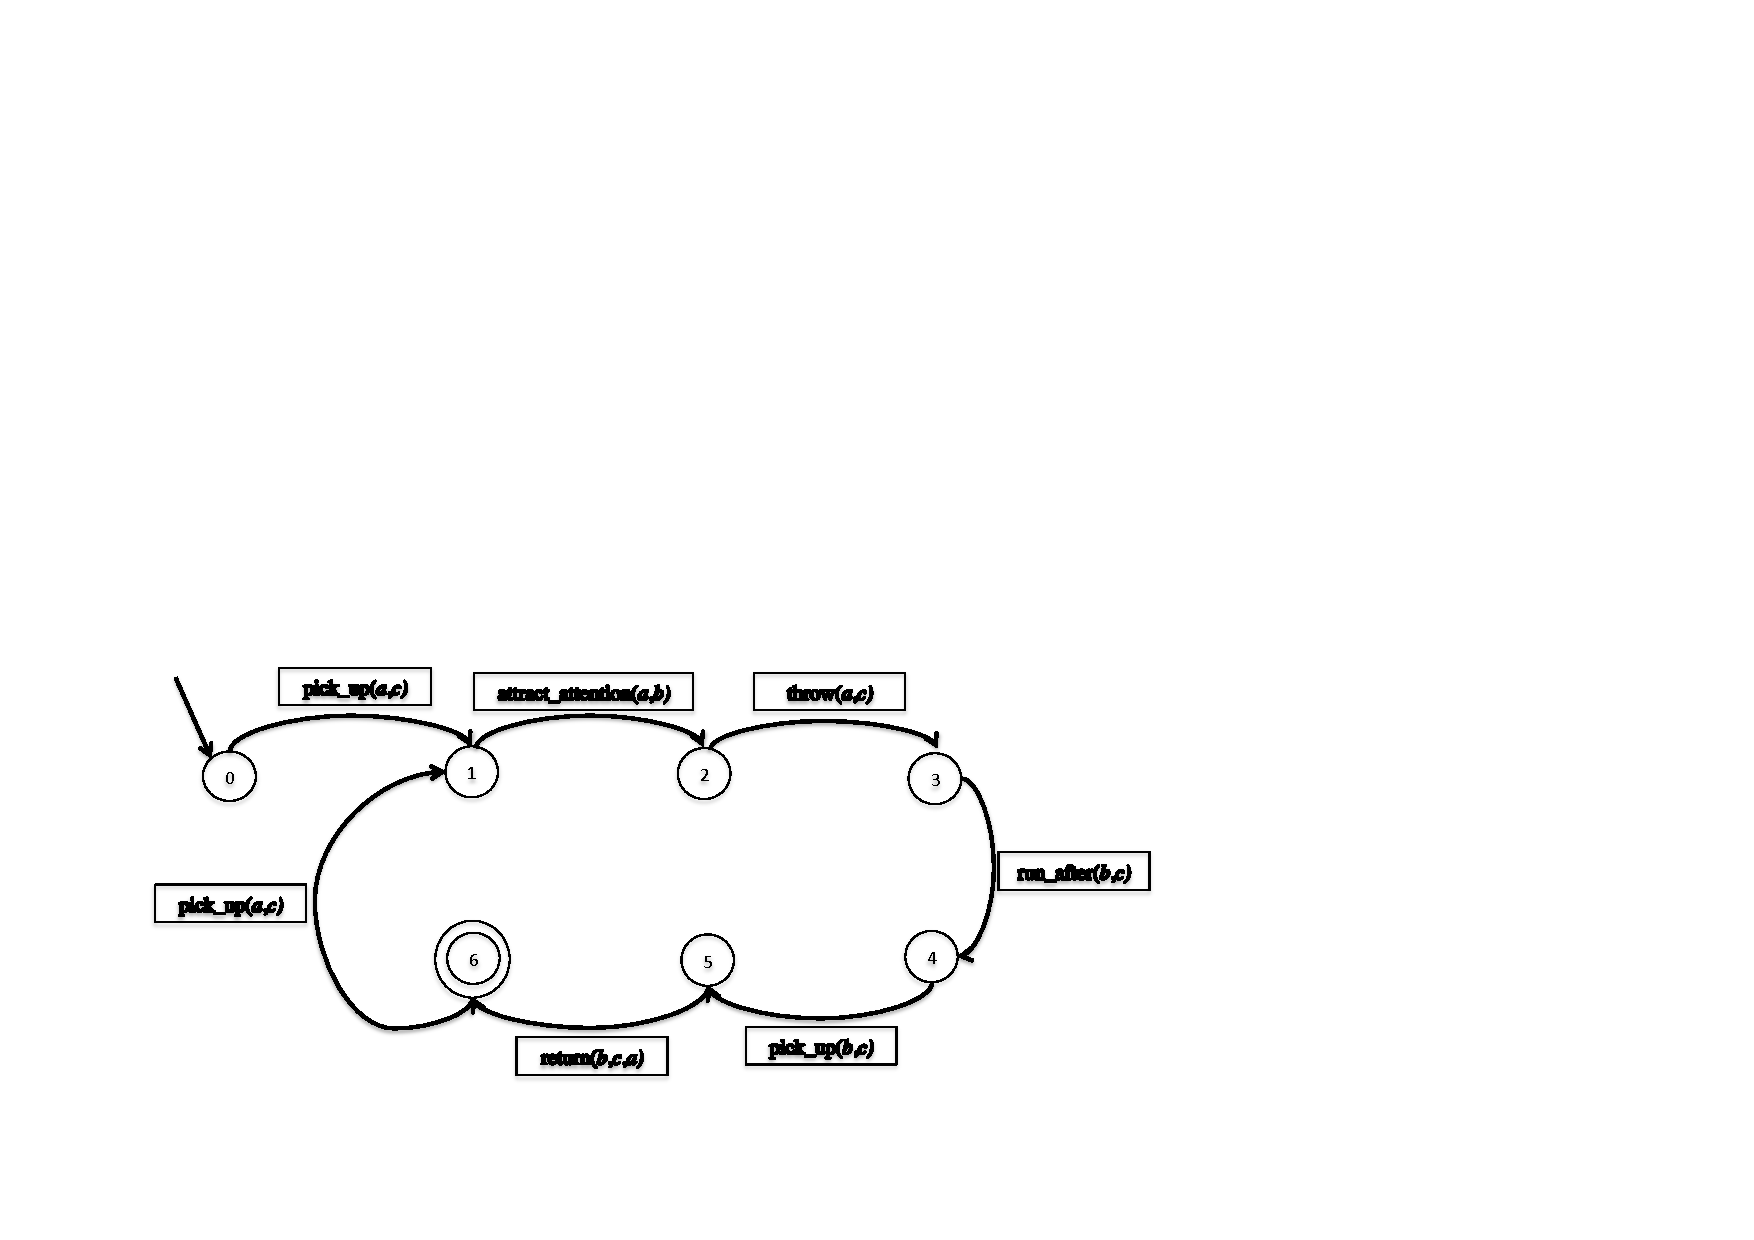
\includegraphics[width=6in]{fetch-fs}

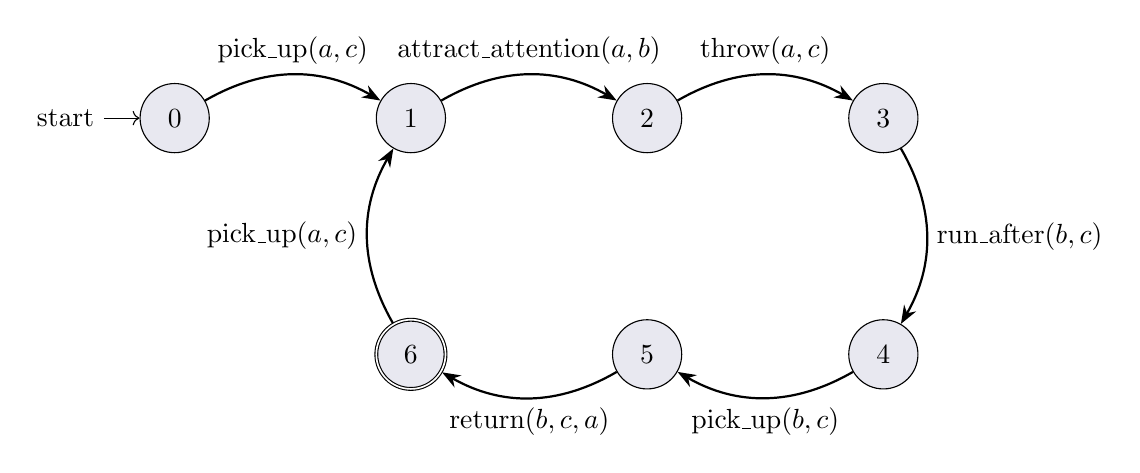
\begin{tikzpicture}[
  node distance=3cm, 
  on grid,
  every state/.style={fill=Lamentation2},
  ]

\node [state, initial] (n0) {0};
\node [state] (n1) [right=of n0] {1};
\node [state] (n2) [right=of n1] {2};
\node [state] (n3) [right=of n2] {3};
\node [state] (n4) [below=of n3] {4};
\node [state] (n5) [left=of n4] {5};
\node [state, accepting] (n6) [left=of n5] {6};

\path [-{Stealth[]}, thick] 
(n0) edge [bend left] node [above] {pick\_up($a,c$)} (n1)
(n1) edge [bend left] node [above] {attract\_attention($a,b$)} (n2)
(n2) edge [bend left] node [above] {throw($a,c$)} (n3)
(n3) edge [bend left] node [right] {run\_after($b,c$)} (n4)
(n4) edge [bend left] node [below] {pick\_up($b,c$)} (n5)
(n5) edge [bend left] node [below] {return($b,c,a$)} (n6)
(n6) edge [bend left] node [left] {pick\_up($a,c$)} (n1);
\end{tikzpicture}


\caption{play\_fetch($a$,$b$,$c$) as a finite state machine}
\label{fig:fetch-fs}
\end{figure}  
Such an automaton will recognize a string of
sub-events.  The idea is that our perception of complex events can be seen as strings of
punctual observations similar to the kind of sampling we are
familiar with from audio technology and digitization processing in
speech recognition.  Thus events can be analyzed as strings of smaller
events.  % What we mean by a string is made precise in
% Appendix~\ref{sec:regular}.
Any object of any type can be part of a
string.  Any two objects (including strings themselves), $s_1$ and $s_2$, can be
\textit{concatenated} to form a string $s_1s_2$.  An
important property of concatenation is \textit{associativity}, that is
if we concatenate $s_1$ with $s_2$ and then concatenate the result
with $s_3$ we get the same string that we would obtain by
concatenating $s_2$ with $s_3$ and then concatenating $s_1$ with the
result.  In symbols: $(s_1s_2)s_3 =
s_1(s_2s_3)$.  For this reason we normally write
$s_1s_2s_3$ (without the parentheses).  Following Fernando we will use these strings to
give us our notion of temporal order.

If $a_1,a_2,\ldots,a_n$ are objects we will normally represent the
string of these objects as $a_1a_2\ldots a_n$.  Where confusion might
arise from this notation we use $\mathrm{str}(a_1a_2\ldots a_n)$.
This latter notation will be particularly useful when distinguishing a
single object, $a$, from a unit string containing this object
$\mathrm{str}(a)$.  Although we will present strings in this way, we will model them as
records \label{pg:stringsasrecords} with distinguished labels related to the natural numbers, 
t$_0$, t$_1$, \ldots (`t' for ``time'').  The field labelled t$_n$
will correspond to the $n+1$th place in the string.  Thus a string of
objects $a_1a_2a_3$
will be the record in \nexteg{}.
\begin{ex} 
\record{\field{t$_0$}{$a_1$} \\
        \field{t$_1$}{$a_2$} \\
        \field{t$_2$}{$a_3$}} 
\end{ex} 
The concatenation of \preveg{} with the string $a_4$, that is, \nexteg{a}, will
be \nexteg{b}.
\begin{ex} 
\begin{subex} 
 
\item \record{\field{t$_0$}{$a_4$}} 
 
\item  \record{\field{t$_0$}{$a_1$} \\
        \field{t$_1$}{$a_2$} \\
        \field{t$_2$}{$a_3$} \\
        \field{t$_3$}{$a_4$}}
 
\end{subex} 
   
\end{ex}

\begin{shaded}
Strings can be introduced into a type system with record types by the
definition in \nexteg{} (repeated in Appendix~\ref{app:strings})
\begin{ex} 
A system of complex types  \textbf{TYPE}$_C$ = $\langle${\bf Type}, {\bf BType},
$\langle$\textbf{PType}, {\bf Pred}, \textbf{ArgIndices}, {\it
  Arity\/}$\rangle$, $\langle A,F\rangle$$\rangle$ with record types
based on $\langle\mathcal{L}, \mathbf{RType}\rangle$ \textit{has strings}
if
\begin{enumerate} 
 
\item for each natural number $i$, t$_i\in\mathcal{L}$
 
\item \textit{String} $\in$ \textbf{BType}

\item $\emptyset:_{\mathbf{TYPE}_C}$ \textit{String}

\item if $T \in$ \textbf{Type} and $a:_{\mathbf{TYPE}_C}T$ then
  $\{\langle\text{t}_0,a\rangle\} : \textit{String}$

\item if $s$ :$_{\mathbf{TYPE}_C}$ \textit{String}, t$_n\in\mathrm{labels}(s)$ such that
  there is no $i>n$ where t$_i\in\mathrm{labels}(s)$, $T \in$ \textbf{Type}
  and $a:_{\mathbf{TYPE}_C}T$ then $s\cup\{\langle \mathrm{t}_{n+1},a\rangle\}$ :$_{\mathbf{TYPE}_C}$
  \textit{String}

\item Nothing is of type \textit{String} except as required above.
 
\end{enumerate}
\label{ex:string-sys} 
\end{ex} 
\preveg{}, clause~1 ensures that the labels $t_i$ are among the labels
available for forming record types.  Clause~2 introduces a basic type
\textit{String}.  Clause~3 says the empty set (also known as the empty
record and empty string) is a string. Clause~4 says that if you have
an object, $a$, of some type then you can form a unit string
containing $a$.  That is the record
\smallrecord{\field{t$_0$}{$a$}}. Note that we always start with the
label `t$_0$'. Clause~5 says that we can always create a new string
from a string $s$ by adding an additional object to the end of it,
using a label `t$_{n+1}$' where $n$ is the highest number such that
$\text{t}_n\in\mathrm{labels}(s)$.  Clause~6 is an exclusion clause.
Clauses~3--6 constitute an inductive definition of the set of
witnesses of the type \textit{String}.

In our informal proof theoretic notation this can be characterized by
giving an inductive definition as in \nexteg{}.
\begin{ex} 
For $\Gamma$ a system of complex types with record types based on
$\langle\mathcal{L},\mathbf{RType}\rangle$ and strings
\begin{subex} 
 
\item \begin{prooftree}
\infer0[$i\in\textit{Nat}$]{\text{t}_i\in\mathcal{L}} 
\end{prooftree} 

\item \begin{prooftree}
\infer0{\Gamma\vdash\textit{String}\in\textbf{BType}}
\end{prooftree}

\item \begin{prooftree}
\infer0{\Gamma\vdash\emptyset:\textit{String}}
\end{prooftree}

\item \begin{prooftree}
\hypo{\Gamma\vdash a:T}
\infer1{\Gamma\vdash\{\langle\text{t}_0,a\rangle\}:\textit{String}}
\end{prooftree} 

\item \begin{prooftree}
\hypo{\Gamma\vdash s:\textit{String}}
\hypo{\Gamma\vdash a:T}
\hypo{\{\text{t}_0,\ldots,\text{t}_n\}=\mathrm{labels}(s)}
\infer3[$n\geq 0$]{\Gamma\vdash
  s\cup\{\langle\text{t}_{n+1},a\rangle\}:\textit{String}}
\end{prooftree}
 
\end{subex} 
   
\end{ex} 
    
\end{shaded} 
We will continue to
represent strings for convenience in the traditional way but modelling
strings as records will become important when following paths in
records down to elements in strings and any operations we define on
records will automatically generalize to strings.  We will use
$\varepsilon$ to represent the empty string (that is, the empty set). We will use $s[n]$ to represent
the $n$th element in a string $s$ (where the first element in the
string is $s[0]$).  In terms of the record notation
this is just a convenient abbreviation for $s$.t$_n$.

\label{pg:stringtype-notation}We will use $T^{=n}$, or, when there is no risk of confusion, simply
$T^n$, as the type of strings of length $n$ all of whose elements are
of type $T$. We will use $T^{\geq n}$ for the type of strings of
objects of type $T$ which have length greater than or equal to $n$.
In particular we will use $T^*$ (the Kleene star) for $T^{\geq0}$ and
$T^+$ (the Kleene plus) for $T^{\geq1}$.

\begin{shaded}
We can make this precise with the definition in \nexteg{} (repeated in
Appendix~\ref{app:strings})
\begin{ex} 
A system of complex types  \textbf{TYPE}$_C$ = $\langle${\bf Type}, {\bf BType},
$\langle$\textbf{PType}, {\bf Pred}, \textbf{ArgIndices}, {\it
  Arity\/}$\rangle$, $\langle A,F\rangle$$\rangle$ with strings has
\textit{length determining string types} if
\begin{enumerate} 
 
\item for any $T\in\textbf{Type}$ and $n$ a natural number, the string
  types $T^{=n}$,
  $T^{\leq n}$, $T^{\geq n}\in\textbf{Type}$ 
 
\item $s:_{\mathbf{TYPE}_C}T^{=n}\ (T^{\leq n}, T^{\geq n})$ iff
  $s:_{\mathbf{TYPE}_C}\textit{String}$, for all $i$, $0\leq
  i<\mathrm{length}(s)$, $s[i]:_{\mathbf{TYPE_C}}T$ and $\mathrm{length}(s) =
  (\leq,\geq)\ n$ 
 
\end{enumerate}
\label{ex:ldstringtypes} 
\end{ex} 

In our informal proof theoretic notation this can be expressed as
\nexteg{}.
\begin{ex} 
For $\Gamma$ a system of complex types with strings and length
determining string types:
\begin{subex} 
 
\item \begin{prooftree}
\hypo{\Gamma\vdash T\in\textbf{Type}}
\infer1[$n\in\textit{Nat}$]{\Gamma\vdash T^{=n}\in\textbf{Type}}
\end{prooftree}
\hspace*{2em}
\begin{prooftree}
\hypo{\Gamma\vdash T\in\textbf{Type}}
\infer1[$n\in\textit{Nat}$]{\Gamma\vdash T^{\leq n}\in\textbf{Type}}
\end{prooftree}
\hspace*{2em}
\begin{prooftree}
\hypo{\Gamma\vdash T\in\textbf{Type}}
\infer1[$n\in\textit{Nat}$]{\Gamma\vdash T^{\geq n}\in\textbf{Type}}
\end{prooftree}
 
 
\item  \begin{prooftree}
\hypo{\Gamma\vdash s:\textit{String}}
\hypo{\mathrm{length}(s)=n}
\hypo{[i<n]}
\ellipsis{}{\Gamma\vdash s[i]:T}
\infer3{\Gamma\vdash s:T^{=n}}
\end{prooftree}
\hspace*{2em}
\begin{prooftree}
\hypo{\Gamma\vdash s:\textit{String}}
\hypo{\mathrm{length}(s)\leq n}
\hypo{[i<\mathrm{length}(s)]}
\ellipsis{}{\Gamma\vdash s[i]:T}
\infer3{\Gamma\vdash s:T^{\leq n}}
\end{prooftree}
\hspace*{2em}
\begin{prooftree}
\hypo{\Gamma\vdash s:\textit{String}}
\hypo{\mathrm{length}(s)\geq n}
\hypo{[i<\mathrm{length}(s)]}
\ellipsis{}{\Gamma\vdash s[i]:T}
\infer3{\Gamma\vdash s:T^{\geq n}}
\end{prooftree} 
\end{subex} 
  
\end{ex}
\preveg{a} introduces the string types and \preveg{b} specifies
witness conditions for the types. 
  
  
\end{shaded}    

Next we introduce concatenation types.  For any
two types, $T_1$ and $T_2$, we can form the type ${T_1}^{\frown}T_2$.
This is the type of strings $ab$ where $a:T_1$ and $b:T_2$.
The concatenation operation on types (just like that on objects) is
associative so we do not use parentheses when more than one type is
involved, e.g. ${T_1}^{\frown}{T_2}^{\frown}T_3$.

\begin{shaded}
This can be made precise as \nexteg{}, repeated in
Appendix~\ref{app:strings}.
\begin{ex} 
A system of complex types  \textbf{TYPE}$_C$ = $\langle${\bf Type}, {\bf BType},
$\langle$\textbf{PType}, {\bf Pred}, \textbf{ArgIndices}, {\it
  Arity\/}$\rangle$, $\langle A,F\rangle$$\rangle$ with strings and
length determining string types has \textit{concatenation types}
if
\begin{enumerate} 
 
\item if $T_1$, $T_2\in\textbf{Type}$ then the string type $T_1^\frown T_2\in\textbf{Type}$ 
 
\item $s:_{\mathbf{TYPE}_C}T_1^\frown T_2$ iff there are $s_1$ and
  $s_2$ such that
\begin{enumerate} 
 
\item $s_1s_2=s$ 
 
\item $s_1:_{\mathbf{TYPE}_C}T_1$ if $T_1$ is a string type, otherwise
  $s_1:_{\mathbf{TYPE}_C}{T_1}^{=1}$

\item $s_2:_{\mathbf{TYPE}_C}T_2$ if $T_2$ is a string type, otherwise
  $s_2:_{\mathbf{TYPE}_C}{T_2}^{=1}$  
 
\end{enumerate} 
   
 
\end{enumerate} 
\label{ex:concatenation-types} 
\end{ex}
Clause~1 introduces concatenation types, $T_1^\frown T_2$, and clause~2 says that
witnesses for concatenative types must be the concatenation of two
strings which are of the types $T_1$ and $T_2$ resepctively if they
are string types of if they are not they must be of the type of
singleton strings whose only element is of type $T_1$ or $T_2$
respectively.  

We can express this in our informal proof theoretic notation as
\nexteg{}.
\begin{ex} 
For $\Gamma$ a system of complex types with strings, length
determining string types and concatenative string types
\begin{subex} 
 
\item \begin{prooftree}
\hypo{\Gamma\vdash T_1\in\textbf{Type}}
\hypo{\Gamma\vdash T_2\in\textbf{Type}}
\infer2{\Gamma\vdash {T_1}^\frown T_2\in\textbf{Type}}
\end{prooftree} 
 
\item \begin{prooftree}
\hypo{\Gamma\vdash s_1:T_1'}
\hypo{\Gamma\vdash s_2:T_2'}
\infer2[$T_i'=T_i$ if $T_i$ is a string type; otherwise
$T_i'=T_i^{=1}$]{\Gamma\vdash s_1s_2:T_1^\frown T_2}
\end{prooftree} 
 
\end{subex} 
   
\end{ex} 
\preveg{a} introduces concatenative types, $T_1^\frown T_2$,  and
\preveg{b} tells us that witnesses for these types are concatenations
of two strings, $s_1$ and $s_2$, where $s_1:T_1$ (or $s_1:T_1^{=1}$ if
$T_1$ is not a string type) and similarly for $s_2$ and $T_2$. 

To \preveg{} we can add \nexteg{} to express the associativity of
`$^\frown$'.
\begin{ex} 
\begin{prooftree}
\hypo{\Gamma\vdash (T_1^\frown T_2)^\frown T_3\in\textbf{Type}}
\hypo{\Gamma\vdash T_1^\frown(T_2^\frown T_3)\in\textbf{Type}}
\infer2{\Gamma\vdash(T_1^\frown T_2)^\frown T_3 =
  T_1^\frown(T_2^\frown T_3)\in\textbf{Type}}
\end{prooftree}
\end{ex} 
   
  

\end{shaded}

While strings as we have defined them are useful for modelling events
in terms of strings of subevents, it is not the case that all strings
of events
can be considered as occurring events.  Consider a case where we have
to events as characterized in \nexteg{}.
\begin{ex} 
\begin{subex} 
 
\item $e_1:T_1$ 
 
\item $e_2:T_2$ 
 
\end{subex} 
   
\end{ex} 
The type theory as we have defined it will yield both
juedgements in \nexteg{}.
\begin{ex} 
\begin{subex} 
 
\item $e_1e_2:T_1^{\frown}T_2$ 
 
\item $e_2e_1:T_2^{\frown}T_1$ 
 
\end{subex} 
   
\end{ex} 
However, if we are using event strings to model temporal ordering it
cannot be the case that both $e_1e_2$ and $e_2e_1$ both model
occurring events even though they are both strings of events.  That
is, if $e_1$ temporally precedes $e_2$ then $e_2$ cannot temporally
precede $e_1$  and \textit{vice versa}.  This has to do with the fact
that a particular event can only happen once.  It is, of course,
possible to have different events of the same types occurring in the
reverse order as in \nexteg{}.
\begin{ex} 
\begin{subex} 
 
\item $e_1e_2:T_1^{\frown}T_2$ 
 
\item $e_3e_4:T_2^{\frown}T_1$ 
 
\end{subex} 
   
\end{ex} 
One way to distinguish those strings which correspond to occurring
events from those which do not is to introduce a type \textit{Occur}
such that if $e_1e_2:\textit{Occur}$ then $e_2e_1\not:\textit{Occur}$.
Below we will use records to model the simultaneous occurrence of
events.  We can do this by allowing records to be witnesses for
\textit{Occur} and requiring that if $r:\textit{Occur}$ and
$\ell_1,\ell_2\in\mathrm{labels}(r)$ then
$r.\ell_1r.\ell_2\not:\textit{Occur}$.  We will not develop this idea
further here but assume it in the background.  

Let us return to Kim watching the boy, $a$, playing fetch with the
dog, $b$, using the stick, $c$. % over a time interval $t$
She
perceives the event as being of type play\_fetch($a$,$b$,$c$).
But what does it mean to be an event of this type?  Given our
concatenation types we can build a type which corresponds to most of
what we have sketched in Figure~\ref{fig:fetch}, namely \nexteg{}.
% (again ignoring time for the sake of simplification).
\begin{ex} 
pick\_up($a$,$c$)$^{\frown}$attract\_attention($a$,$b$)$^{\frown}$throw($a$,$c$)$^{\frown}$run\_after($b$,$c$)$^{\frown}$pick\_up($b$,$c$)$^{\frown}$\\
\hspace*{2em}return($b$,$c$,$a$) 
\end{ex} 
\preveg{} is a type corresponding to everything we have represented in
Figure~\ref{fig:fetch} except for the arrow which loops back from the
end state to the start state.    In order to get the loop into the event
type we will use a Kleene-+ type.  % In
% standard notations for strings $s^+$ stands for a string consisting of
% one or more occurrences of $s$.\footnote{This notation was introduced
%   by the mathematician Stephen Kleene.}
% We will adopt this into types
% by saying that for any type $T$ there is also a type $T^+$ which is
% the type of strings of objects of type $T$ containing one or more
% members.  (See Appendix~\ref{sec:regular} for a more precise
% definition.)
The type \nexteg{} will, then,
give us a type corresponding to the complete Figure~\ref{fig:fetch}
since it will be the type consisting of strings of one or more events
of the type \preveg{}.
\begin{ex} 
(pick\_up($a$,$c$)$^{\frown}$attract\_attention($a$,$b$)$^{\frown}$throw($a$,$c$)$^{\frown}$run\_after($b$,$c$)$^{\frown}$pick\_up($b$,$c$)$^{\frown}$
\\ \hspace*{2em}return($b$,$c$,$a$))$^+$ 
\end{ex}


% In \preveg{} we simplified the string type by excluding time.  Now we
% will consider what is needed to put time back in.  Each of the
% subevents represented there is associated with a time interval, a
% different time interval for each subevent.  The type for time
% intervals, which we will abbreviate as \textit{TimeInt} is \nexteg{}\label{pg:TimeInt}.
% \begin{ex} 
% \record{\tfield{start}{\textit{Time}} \\
%         \tfield{end}{\textit{Time}} \\
%         \tfield{c$_<$}{start$<$end}}
% \end{ex} 
% where \textit{Time} is the type of time points and $<$ is the relation
% ``earlier than'' defined on the witnesses of this type.\footnote{We
%   use the infix notation $t_1<t_2$ rather than the official notation
%   $<(t_1,t_2)$.}  In order to get time intervals associated with each
% subevent we will treat the subevent types as record types rather than
% ptypes.  Thus as a first step towards characterizing the right type we
% have \nexteg{}.
% \begin{ex} 
% \smallrecord{\smalltfield{e-time}{\textit{TimeInt}} \\
%              \smalltfield{c$_{\mathrm{pick\_up}}$}{pick\_up($a$,$c$,e-time)}}$^{\frown}$\smallrecord{\smalltfield{e-time}{\textit{TimeInt}}
%              \\
%                   \smalltfield{c$_{\mathrm{attract\_attention}}$}{attract\_attention($a$,$b$,e-time)}}$^{\frown}$

% \medskip
% \smallrecord{\smalltfield{e-time}{\textit{TimeInt}} \\
%              \smalltfield{c$_{\mathrm{throw}}$}{throw($a$,$c$,e-time)}}$^{\frown}$\smallrecord{\smalltfield{e-time}{\textit{TimeInt}} \\
%              \smalltfield{c$_{\mathrm{run\_after}}$}{run\_after($b$,$c$,e-time)}}$^{\frown}$

% \medskip
% \smallrecord{\smalltfield{e-time}{\textit{TimeInt}} \\
%              \smalltfield{c$_{\mathrm{pick\_up}}$}{pick\_up($b$,$c$,e-time)}}$^{\frown}$\smallrecord{\smalltfield{e-time}{\textit{TimeInt}} \\
%              \smalltfield{c$_{\mathrm{return}}$}{return($b$,$c$,$a$,e-time) }}
% \end{ex}

% This will get us a time interval for each subevent but it does not
% require any relationship between the time intervals of the different
% subevents whereas, of course, each subevent should occur at a later
% time than the previous one.  In order to achieve this we will
% introduce a more restricted notion of type concatenation especially
% for record types which have a field
% \smallrecord{\smalltfield{e-time}{\textit{TimeInt}}} as in \nexteg{}.
% \begin{ex}
% \begin{enumerate} 
% \item If $T_1$ and $T_2$ are subtypes of
% \smallrecord{\smalltfield{e-time}{\textit{TimeInt}}}$^+$ then
% $T_1^{\frown_<}T_2$ is a type. 

% \item $a:T_1^{\frown_<}T_2$ iff $a=a_1^{\frown}a_2$, $a_1:T_1$, $a_2:T_2$ and
%   last($a_1$).e-time.end$<$first($a_2$).e-time.start
% \end{enumerate}
% \end{ex} 
% Here first($s$) and last($s$) pick out the first and last elements
% respectively of the string $s$.  We need to make a similar adjustment
% to the Kleene-+ type constructor.
% \begin{ex} 
% \begin{enumerate} 
 
% \item If $T$ is a subtype of
%   \smallrecord{\smalltfield{e-time}{\textit{TimeInt}}} then $T^{+_<}$
%   is a type
 
% \item $a:T^{+_<}$ iff $a=x_1^\frown\!\ldots^\frown\!x_n$, $n>0$ and
%   for $i$, $j$, $1\leq
% i<j\leq n$, $x_i:T$, $x_j:T$ and $x_i^{\frown}x_j:T^{\frown_<}T$ 
 
% \end{enumerate} 
   
% \end{ex} 

% [The details of temporal concatenation above should be included in the
% appendix.]

We will complicate \preveg{} slightly by substituting record types for
the ptypes as in \nexteg{}.  We do this because we
will want to allow for things happening simultaneously and record
types will give us a straightforward way of allowing this.
\begin{ex} 
(\smallrecord{\smalltfield{e}{pick\_up($a$,$c$)}}$^{\frown}$\smallrecord{\smalltfield{e}{attract\_attention($a$,$b$)}}$^{\frown}$\smallrecord{\smalltfield{e}{throw($a$,$c$)}}$^{\frown}$\smallrecord{\smalltfield{e}{run\_after($b$,$c$)}}$^{\frown}$\\
\hspace*{2em}\smallrecord{\smalltfield{e}{pick\_up($b$,$c$)}}$^{\frown}$\smallrecord{\smalltfield{e}{return($b$,$c$,$a$)}})$^+$ 
\label{eg:fetch-type}
\end{ex}
The label `e' (``event'') occurs in each of the elements of the string
type.  In this case we will say that `e' labels a \textit{dimension}
of events of this type.  The `e'-dimension can be thought of as the
dimension which characterizes what is happening at each stage of the
event.  % If you want to think geometrically, you can think of the
% event-string as being located in a space of event types (that is, the ptypes).

% So now we can represent the event type for playing fetch as \nexteg{}.
% \begin{ex} 
% (\smallrecord{\smalltfield{e-time}{\textit{TimeInt}} \\
%              \smalltfield{c$_{\mathrm{pick\_up}}$}{pick\_up($a$,$c$,e-time)}}$^{\frown_<}$\smallrecord{\smalltfield{e-time}{\textit{TimeInt}}
%              \\
%                   \smalltfield{c$_{\mathrm{attract\_attention}}$}{attract\_attention($a$,$b$,e-time)}}$^{\frown_<}$

% \medskip
% \smallrecord{\smalltfield{e-time}{\textit{TimeInt}} \\
%              \smalltfield{c$_{\mathrm{throw}}$}{throw($a$,$c$,e-time)}}$^{\frown_<}$\smallrecord{\smalltfield{e-time}{\textit{TimeInt}} \\
%              \smalltfield{c$_{\mathrm{run\_after}}$}{run\_after($b$,$c$,e-time)}}$^{\frown_<}$

% \medskip
% \smallrecord{\smalltfield{e-time}{\textit{TimeInt}} \\
%              \smalltfield{c$_{\mathrm{pick\_up}}$}{pick\_up($b$,$c$,e-time)}}$^{\frown_<}$\smallrecord{\smalltfield{e-time}{\textit{TimeInt}} \\
%              \smalltfield{c$_{\mathrm{return}}$}{return($b$,$c$,$a$,e-time) }})$^{+_<}$
% \end{ex}


\section{Doing things with types}
\label{sec:typeacts}

\subsection{Type acts}

The boy and the dog have to coordinate and interact in order to create an
event of the game of fetch.  This involves doing more with types than
just making judgements.  For example, when the dog observes the
situation in which the boy raises the stick, it may not be clear
to the dog whether this is part of a fetch-game situation or a
stick-beating situation.  The dog may be in a situation of
entertaining these two types as possibilities prior to making the
judgement that the situation is of the fetch type.  We will call this
act a query as opposed to a judgement.  Once the dog has made the
judgement that what it has observed so far is an initial segment of a
fetch type situation it has to make its own contribution in order to
realize the fetch type, that is, it has to run after the stick and
bring it back.  This involves the creation of a situation of a certain
type.  Thus creation acts are another kind of act related to types.
Creating objects of a given type often has a \textit{de se}
\citep[see, for example,][]{Perry1979,Lewis1979a,Ninan2010,Schlenker2011} aspect.  The dog
has to know that it itself must run after the stick in order to make
this a situation in which it and the boy are playing fetch.  There is
something akin to what Perry calls an essential indexical here,
though, of course, the dog does not have indexical linguistic
expressions. It is nevertheless part of the basic competence that an
agent needs in order to be able to coordinate its action with the rest
of the world that it has a primitive sense of self which is distinct
from being able to identify an object which has the same properties as
itself.  We will follow Lewis in modelling \textit{de se} in terms of
functional abstraction over the ``self''.  In our terms this will mean
that \textit{de se} type acts involve dependent types.

In standard type theory we have judgements such as $o:T$ ``$o$ is of type $T$'' 
and 
$T$ \textit{true} ``there is something of type $T$''.    We want to
enhance this notion of judgement by including a reference to the agent
$A$ which makes the judgement, giving judgements such as
$o:_AT$ ``agent $A$ judges that $o$ is of type $T$''
and 
$:_AT$ ``agent $A$ judges that there is some object of type $T$''. We will call
the first of these a \textit{specific} judgement and the second a
\textit{non-specific} judgement.  Such
judgements are one of the three kinds of acts represented in \nexteg{}
that we want to include
in our type act theory.
\begin{ex} 
\textit{Type Acts}
\begin{description}
\item[judgements] \mbox{}

\begin{description}
\item[\textit{specific}] $o:_A T$ ``agent $A$ judges object $o$ to be of type
  $T$''

\item[\textit{non-specific}] $:_A T$ ``agent $A$ judges that there is some
  object of type $T$''
\end{description}

\item[queries] \mbox{}
\begin{description}
\item[\textit{specific}] $o:_A T?$ ``agent $A$ wonders whether object $o$ is of type
  $T$''

\item[\textit{non-specific}] $:_A T?$ ``agent $A$ wonders whether there is some object of type
$T$''
\end{description}
\item[creations] \mbox{}
\begin{description}
\item[\textit{non-specific}] $:_A T!$ ``agent $A$ creates something of type
  $T$''
\end{description}
\end{description}

\end{ex} 
Note that creations only come in the non-specific variant.  You cannot
create an object which already exists.  

Creations are also limited in
that there are certain types which a given agent is not able to
realize as the main actor.  Consider for example the event type involved in the fetch
game of the dog running after the stick.  The human cannot be the main
creator of such
an event since it is the dog who is the actor.  The most the human can
do is wait until the dog has carried out the action
and we will count this as a creation type act.  This will become
important when we discuss coordination in the fetch-game below.  It is
actually important that the human makes this passive contribution to
the creation of the event of the dog running after the stick and does
not, for example, get the game confused by immediately throwing
another stick before the dog has had a chance to retrieve the first
stick.  There are other cases of event types which require a less
passive contribution from an agent other than the main actor.
Consider the type of event where the dog returns the stick to the
human.  The dog is clearly the main actor here but the human has also
a role to play in making the event realized.  For example, if the
human turns her back on the dog and ignores what is happening or runs
away, the event type will not be realized despite the dog's best
efforts.  Other event types, such as lifting a piano, involve more
equal collaboration between two or more agents, where it is not
intuitively clear that any one of the agents is the main actor.  So
when we say ``agent $A$ creates something of type $T$'' perhaps it
would be more accurate to phrase this as ``agent $A$ contributes to
the creation of something of type $T$'' where $A$'s contribution might
be as little as  not realizing any of the other types involved in the game until
$T$ has been realized.   
   
\textit{De se} type acts involve functions which have the agent in its
domain and return a type, that is, they are dependent types which,
given the agent, will yield a type.  We will say that agents are of
type \textit{Ind} and that the relevant dependent types, 
$\mathcal{T}$, are functions of type
  (\textit{Ind}$\rightarrow$\textit{Type}).  
We characterize \textit{de se} type acts in a way parallel to
\preveg{}, as given in \nexteg{}.
\begin{ex}
\textit{De Se Type Acts} 
\begin{description}
\item[\textit{judgements}] \mbox{}
\begin{description}
\item[\textit{specific}]  $o:_A \mathcal{T}(A)$ ``agent $A$ judges object $o$ to be of type
  $\mathcal{T}(A)$''
\item[\textit{non-specific}] $:_A \mathcal{T}(A)$ ``agent $A$ judges
  that there is some object of type $\mathcal{T}(A)$''
\end{description}

\item[\textit{queries}] \mbox{}
\begin{description}
\item[\textit{specific}] $o:_A \mathcal{T}(A)?$ ``agent $A$ wonders whether object $o$ is of type
  $\mathcal{T}(A)$''
\item[\textit{non-specific}] $:_A \mathcal{T}(A)?$ ``agent $A$ wonders whether there is some object of type
$\mathcal{T}(A)$''
\end{description}

\item[\textit{creations}] \mbox{}
\begin{description}
\item[\textit{non-specific}] $:_A \mathcal{T}(A)!$ ``agent $A$ creates
  something of type $\mathcal{T}(A)$''
\end{description}
\end{description} 
\end{ex} 

From the point of view of the type theory \textit{de se} type acts
seem more complex than non-\textit{de se} type acts since they involve
a dependent rather than a non-dependent type and a functional
application of that dependent type to the agent.  However, from a
cognitive perspective one might expect \textit{de se} type acts to be
more basic.  Agents which perform type acts using types directly
related to themselves are behaving egocentrically and one could regard
it as a more advanced level of abstraction to consider types which are
independent of the agent.  This seems a puzzling way in which our
notions of type seem in conflict with out intuitions about cognition.   

While these type acts are prelinguistic (we need them to account for
the dog's behaviour in the game of fetch), it seems
that they are the basis on which the notion of speech act
\citep[and much subsequent literature]{Austin1962,Searle1969} is built.  % Our notion of using types in
% query acts seems intuitively related to work on inquisitive semantics
% \citep{GroenendijkRoelofsen2012} where some propositions (in
% particular disjunctions) are regarded as inquisitive.  However, this
% will still allow us to make a distinction between questions and
% assertions in natural language as argued for by \cite{Ginzburg2012}.

\subsection{Making inferences about events}
What happens
when Kim perceives an event as being of the type (\ref{eg:fetch-type})?  She
makes a series of observations of events, assigning them to types in
the string type.  Note that the ptypes in each of the types can be
further broken down in a similar way.  This gives us a whole hierarchy
of perceived events which at some point have to bottom out in basic
perceptions which are not further analyzed.  In order to recognize an
event as being of this type Kim does not need to perceive a string of
events corresponding to each of the types in the string types.  She
may, for example, observe the boy waving the stick to attract the
dog's attention, get distracted by a bird flying overhead for a while,
and then return to the fetch event at the point where the dog is
running back to the boy with the stick.  This still enables her to
perceive the event as an event of fetch playing because she has seen
such events before and learned that such events are of the string type in (\ref{eg:fetch-type}).  It suffices for her to observe enough of the elements in
the string to distinguish the event from other event types she may
have available in her knowledge resources.  Suppose, for example, that
she has just two event string types available that begin with the picking
up of a stick by a human in the company of a dog.  One is (\ref{eg:fetch-type}).
The other is one that leads to the human beating the dog with the
stick.  If she only observes the picking up of the stick she cannot be
sure whether what she is observing is a game of fetch or a beating.
However, as soon as she observes something in the event string which
belongs only to the fetch type she can reasonably conclude
that she is observing an event of the fetch type.  She may, of course,
be wrong.  She may be observing an event of a type which she does not
yet have available in her resource of event types, in which case she
will need to learn about the new event type and add it to her
resources.  However, given the resources at her disposal she can make
a prediction about the nature of the rest of the event.  One could
model her prediction making ability in terms of a function which maps
a situation (modelled as a record) to a type of predicted situation,
for example \nexteg{}.
\begin{ex} 
$\lambda r$:\smallrecord{\smalltfield{x}{\textit{Ind}} \\
                         \smalltfield{c$_{\mathrm{human}}$}{human(x)}
                         \\
                         \smalltfield{y}{\textit{Ind}} \\
                         \smalltfield{c$_{\mathrm{dog}}$}{dog(y)} \\
                         \smalltfield{z}{\textit{Ind}} \\
                         \smalltfield{c$_{\mathrm{stick}}$}{stick(z)}
                         \\
                         \smalltfield{e}{\smallrecord{
             \smalltfield{e}{pick\_up(x,z)}}$^{\frown}$\smallrecord{
                  \smalltfield{e}{attract\_attention(x,y)}}}} .
            \\*[.75\baselineskip]
\hspace*{4em}\smallrecord{\smalltfield{e}{play\_fetch($r$.x,$r$.y,$r$.z)}
\\
\smalltfield{c$_{\mathrm{init}}$}{init($r$.e,e)}}
\label{ex:ev-predict-fun}
\end{ex} 
% \begin{ex} 
% $\lambda r$:\smallrecord{\smalltfield{x}{\textit{Ind}} \\
%                          \smalltfield{c$_{\mathrm{human}}$}{human(x)}
%                          \\
%                          \smalltfield{y}{\textit{Ind}} \\
%                          \smalltfield{c$_{\mathrm{dog}}$}{dog(y)} \\
%                          \smalltfield{z}{\textit{Ind}} \\
%                          \smalltfield{c$_{\mathrm{stick}}$}{stick(z)}
%                          \\
%                          \smalltfield{e-time}{\textit{TimeInt}} \\
%                          \smalltfield{e}{\smallrecord{\smalltfield{e-time}{\textit{TimeInt}}
%                              \\
% \smalltfield{c$_{\leq}$}{$\Uparrow$e-time.start$\leq$e-time.start} \\
%              \smalltfield{c$_{\mathrm{pick\_up}}$}{pick\_up($\Uparrow$x,$\Uparrow$z,e-time)}}$^{\frown_<}$\smallrecord{\smalltfield{e-time}{\textit{TimeInt}}
%              \\
% \smalltfield{c$_{\leq}$}{e-time.start$\leq\Uparrow$e-time.start} \\
%                   \smalltfield{c$_{\mathrm{attract\_attention}}$}{attract\_attention($\Uparrow$x,$\Uparrow$y,e-time)}}}}
%             \\*[.75\baselineskip]
% \hspace*{4em}(\smallrecord{\smalltfield{e-time}{\textit{TimeInt}} \\
%                            \smalltfield{c$_{\leq}$}{$r$.e-time.start$\leq$e-time.start} \\
%                            \smalltfield{e}{play\_fetch($r$.x,$r$.y,$r$.z,e-time)}})
% \label{ex:ev-predict-fun}
% \end{ex}

Here the predicate `init' has arity
$\langle$\textit{String}, \textit{String}$\rangle$.  The type init($s_1$,$s_2$) is
non-empty just in case $s_1$ is an initial substring of $s_2$.  

\begin{shaded}
We
achieve this by the definition in \nexteg{}, repeated in Appendix~\ref{app:strings}.
\begin{ex}
If $s_1$ is a string of length $n$ and $s_2$ is a string of any
length, then $s$ : init($s_1$,$s_2$) iff the length of $s_2$ is
greater than or equal to $n$ and for each $i$, $0\leq i<n$,
$s_1[i]=s_2[i]$ and $s=s_2$.
\end{ex}
That is, if the initial substring condition holds then the second
argument to the predicate (and nothing else) is of the ptype.
\end{shaded}

% Here a `$\Uparrow$' prefixed to a path-name consisting of labels such
% as `e-time.start' or `x' means that the path-name is to start in the
% next higher record type in which the current record type is embedded.
% This notation is an abbreviation for something much less readable (but
% more precise) which is given in Appendix~\ref{app:rectypes}. [????
% This notation needs to be added to the appendix.]

The kind of function of which (\ref{ex:ev-predict-fun} is an instance is a function
of the general form \nexteg{}.
\begin{ex} 
$\lambda a\!:\!T_1\ .\ T_2\dep{a}$
\label{ex:deptypefun} 
\end{ex} 


Recall that the notation $T_2\dep{a}$ represents that $T_2$
depends on $a$. The nature of this dependence in
(\ref{ex:ev-predict-fun}) is seen in the occurrences of $r$ in the body
of the function, for example, \nexteg{}.
\begin{ex}
play\_fetch($r$.x,$r$.y,$r$.z)
\end{ex}
A function of the form (\ref{ex:deptypefun}) maps an object of some type (represented by $T_1$) to
a type (represented by $T_2\dep{a}$).  The type that results from an
application of this function will depend on what object it is applied
to -- that is, we have the possibility of obtaining different types
from different objects. This function is then a dependent type as
discussed, for example, on p.~\pageref{pg:deptype},  These functions will play an important
role in much of what is to come later in this book.  They will show up
many times in what appear at first blush to be totally unrelated
phenomena.  We want to suggest, however, that all of the phenomena we
will describe using such functions have their origin in our basic
cognitive ability to make predictions on the basis of partial
observation of objects and events.


Functions which are dependent types return types but they do not, of
themselves, tell us what to do with the type if we have obtained it by
applying the function to an argument.  Suppose $\mathcal{T}$ is the
function (\ref{ex:ev-predict-fun}) and that $T$ is the domain type of
$\mathcal{T}$, that is, \nexteg{}.
\begin{ex} 
\smallrecord{\smalltfield{x}{\textit{Ind}} \\
                         \smalltfield{c$_{\mathrm{human}}$}{human(x)}
                         \\
                         \smalltfield{y}{\textit{Ind}} \\
                         \smalltfield{c$_{\mathrm{dog}}$}{dog(y)} \\
                         \smalltfield{z}{\textit{Ind}} \\
                         \smalltfield{c$_{\mathrm{stick}}$}{stick(z)}
                         \\
                         \smalltfield{e}{\smallrecord{
             \smalltfield{e}{pick\_up(x,z)}}$^{\frown}$\smallrecord{
                  \smalltfield{e}{attract\_attention(x,y)}}}} 
\end{ex} 
Then we may have the action rule given in \nexteg{}.
\begin{ex} 
\begin{prooftree}
\hypo{s:_A T}
\infer[enth]1{:_A\mathcal{T}(s)}
\end{prooftree} 
\end{ex} 
\preveg{} represents that if an agent, $A$, judges a situation, $s$, to
be of type $T$ then $A$ is licensed to judge that there is some
situation of type $\mathcal{T}(s)$.  We use a wavy line in this
inference rule to indicate that it does not represent a conclusion
that follows from a premise in a logical sense, but rather that the
act above the line licenses the act below the line.  That is, on the
basis of what is above the line it is reasonable to perform what is
below the line, though without a guarantee that it is correct or even
that the action will be performed.  Given
that you observe a human pick up a stick and attract a dog's
attention, it is reasonable to conclude that there will be an event of
playing fetch, but there is no guarantee that there actually will be
such an event.  We have talked in terms of what is above the line
licensing what is below the line.  Another term that can be used is
\textit{afford} which goes back to Gibson's (\citeyear{Gibson1979})
notion of affordance.  Thus we can talk of the action above the line
as affording the action below the line. 

Sometimes dependent type functions like $\mathcal{T}$ can be
associated with more than one action rule.  Agents may get to choose
which they apply or perhaps there will be aspects of the context which
will determine which of the action rules is appropriate.  Thus in
addition to \preveg{} we might also have the action rules in
\nexteg{}.
\begin{ex} 
\begin{subex} 
 
\item  \begin{prooftree}
\hypo{s:_A T}
\infer[enth]1{s:_A\mathcal{T}(s)}
\end{prooftree}
 
\item \begin{prooftree}
\hypo{s:_A T}
\infer[enth]1{:_A\mathcal{T}(s)!}
\end{prooftree} 
 
\end{subex} 
   
\end{ex} 
\preveg{a} says that if $A$ judges $s$ to be of type $T$ then $A$ is
licensed to judge that $s$ is also of type $\mathcal{T}(s)$.
\preveg{b} says that if $A$ judges $s$ to be of type $T$ then $A$ is
licensed to create something of type $\mathcal{T}(s)$.   

What happens when Kim does not observe enough of the event to be able
to predict with any certainty that the complete event will be a game
of fetch?  One theory would be that she can only make categorical
judgements, and that she has to wait until she has seen enough so that
there is only one type that matches in the collection of situation
types in her resources.  Another theory would be
one where she predicts a disjunction of the available matching types when there is
more than one that matches.  One might refine this theory so that she
can choose one of the available types but assign it a probability
based on the number of matching types.  If $n$ is the number of
matching types the probability of any one of them might be
$\frac{1}{n}$.  This assumes that each of the types is equally likely
to be realized.  It would be natural to assume, however, that the
probability which Kim assigns to any one of the matching types would
be dependent on her previous experience.  Suppose, for example, that
she has seen 100 events of a boy picking up a stick in the company of
a dog, 99 of those events led to a game of fetch and only one led to
the boy beating the dog.  One might then assume that when she now sees
the boy pick up the stick she would assign a .99 probability (on a
scale of 0 to 1) to the
type of fetch events and only .01 probability to the boy beating the
dog.  That is, the probability she assigns to an event of a boy
picking up a stick leading to a game of fetch is the result of
dividing the number of instances of a game of fetch she has already
observed by the sum of the number of instances she has observed of any types whose
initial segment involves the picking up of a stick.  In more general
terms we can compute the probability which an agent $A$ assigns on the
basis of a string, $s$, of previous observations to a
predicted type $T_{\mathit{pr}}$ given an observed type $T_{\mathit{obs}}$, $p_{A,\omega}(T_{\mathit{pr}}\mid T_{\mathit{obs}})$, in the case where
$T_{\mathit{pr}}$ is a member of the set of alternatives which can be
predicted from $T_{\mathit{obs}}$ according to $A$'s resources based on $p$,
$\mathrm{alt}_{A,s}(T_{\mathit{obs}})$, by the formula in
\nexteg{}.
\begin{ex}
$p_{A,s}(T_{\mathit{pr}}\mid T_{\mathit{obs}}) =
\frac{\mid\{T_{\mathit{pr}}\}^{A,s}\mid}{\sum\limits_{T_{\mathit{alt}}\in\mathrm{alt}_{A,s}(T_{\mathit{obs}})}\mid\{T_{\mathit{alt}}\}^{A,s}\mid}$
\end{ex}
where $\{T\}^{A,s}$ is the set of objects of type $T$ observed by $A$
in $s$.  If $T_{\mathit{pr}}$ is not a member of
$\mathrm{alt}_{A,s}(T_{\mathit{obs}})$, that is not one of the
alternatives, we say that $p_{A,s}(T_{\mathit{pr}}\mid
T_{\mathit{obs}}) = 0$.  

Where does the set of alternatives come from?  We assume that an agent
has a set of functions similar to (\ref{ex:ev-predict-fun}) available
as cognitive resources, that is, a set of resources that associates
objects of given types with another type, that is collections of
dependent types.  We could think of these
resources as topoi in the sense of \cite{Breitholtzfthca}.  Among this collection of functions may be several which
share the same domain type, that is, for some particular type $T$ they
are witnesses of the function type $(T\rightarrow\textit{Type})$.
Suppose that $F$ is a set of such resources sharing the type $T$ as a
domain type.  Then the set of alternatives for an object $r$ of type
$T$ with respect to $F$ is $\{T'\mid T'=f(r)\text{ for some } f\in F\}$. 

While this is still a rather naive and simple view of how
probabilities might be assigned it is not without interest, as shown
by the following points:  
\paragraph{Probability distributions} It will always provide a probability distribution over sets
of alternatives, that is \nexteg{}.
\begin{ex}
$\sum\limits_{T_{\mathit{pr}}\in\mathrm{alt}_{A,s}(T_{\mathit{obs}})}p_{A,s}(T_{\mathit{pr}}\mid
T_{\mathit{obs}}) = 1$
\end{ex}
\paragraph{Alternatives} We have assumed a notion of alternatives based on types of completed
events for which the observed event is an initial segment but other
notions of alternativeness could be considered and perhaps even
combined.  
\paragraph{Relativity of probability assignments} The notion of
probability is both agent and resource relative.  It represents the
probability which an agent will assign to a type when observing a
given situation after a previous string of observations.  Two agents may assign different
probabilities depending on the resources they have available.
\paragraph{Learning} Relevant observations will update the probability
distributions an agent will assign to a given set of alternatives
since the probability is computed on the basis of previous
observations of the alternative types.

Kim is not alone in being able to draw conclusions based on partial
observations of an event.  The dog can do it too.  As soon as the boy
has raised the stick and attracted the dog's attention the dog is
excitedly snapping at the stick and starting to run in the direction
in which the boy seems to be about to throw.  The dog also seems to be
attuned to string types of events just as Kim is and also able to make
predictions on the basis of partial observations.  The types to which
a dog is attuned will not be the same as those to which humans can be
attuned and this can certainly lead to miscommunication between humans
and dogs.  For example, there may be many reasons why I would go to
the place where outdoor clothes are hanging and where the dog's lead
is kept.  Many times it will be because I am planning to take the dog
out for a walk, but not as often as the dog appears to think, judging
from the excitement he shows any time I go near the lead.  It is
difficult to explain to the dog that I am just looking for a receipt
that I think I might have left in my coat pocket.  But the basic
mechanism of being able to assemble types of events
into string types of more complex events and make predictions on the
basis of these types seems to be common to both humans and dogs and a
good number of other animals too.  Perhaps simple organisms do not
have this ability and can only react to events that have already
happened, but not to predicted outcomes.

This basic inferential ability is thus not parasitic on the ability to
communicate using a human language.  It is, however, an ability which
appears to be exploited to a great extent in our use of language as we
will see in later chapters.  


% When talking about the intuition behind this
% analysis Fernando sometimes refers to strings of frames in a movie
% (e.g. in \cite{Fernando2008}).  But in many cases what he is calling
% a movie frame 
% can also be seen as a frame in something like the sense of frame semantics as well.

\subsection{Coordination and games}

Let us now apply these notions to the kind of interaction that has to
take place between the human and the dog in a game of fetch.  First
consider in more detail what is actually involved in playing a game of
fetch, that is creating an event of type (\ref{eg:fetch-type}).  Each
agent has to keep track in some way of where they are in the game and
in particular what needs to happen next.  We analyze this by saying
that each agent has an information state which we will model as a
record.  We need to keep track of the progression of types of
information state for an agent during the course of the game.  We will
refer to the types of information states as gameboards.\footnote{Our
  notions of \textit{information state} and \textit{gameboard} are
  taken from \cite{Larsson2002} and \cite{Ginzburg2012} respectively
  as well as a great deal of related literature on the gameboard or
  information state approach to dialogue analysis originating from
  \cite{Ginzburg1994}.  We have adapted the notions somewhat to our own
  purposes.}  The idea is that as part of the event
occurs, the agent's gameboard is updated so that an event of the
next type in the string is expected.  For now, we will consider
gameboards which only place one requirement on information states,
namely that there is an agenda which indicates the type of the next
move in the game.  Thus if the agent is playing fetch and observes an
event of the type where the human throws the stick, then, according to
(\ref{eg:fetch-type}), the next move in the game will be an event of
the type where the dog runs after the stick.  If the actor in the next
move is the agent herself then the agent will need to create an event
of the type of the next move if the game is to progress.  If the actor in the next move is the
other player in the game, then the agent will need to observe an event
and judge it to be of the appropriate type in order for the game to
progress.  The type of information states, \textit{InfoState}, will be
\nexteg{a}.    The type of the initial
information state, \textit{InitInfoState}, will be one where the agenda is required to be the
empty list.  % We use $\mathrm{list}(T)$ to represent the type of lists
% of objects of type $T$ and [ ] to represent the empty list.  We use
% $\mathrm{fst}(L)$ to represent the first member of the list and
% $\mathrm{rst}(L)$ to represent the rest of the list, that is, the list
% of all the members of list except the first.
\begin{ex}
\begin{subex} 
\item \record{\tfield{agenda}{$\mathrm{list}(\textit{RecType})$}}
\item \record{\mfield{agenda}{[ ]}{$\mathrm{list}(\textit{RecType})$}} 
\end{subex}
\label{ex:InfoState-InitInfoState}
\end{ex}
The type \textit{RecType} is the type of record types, that is, the
witnesses for this type will be record types.  Just like the type
\textit{Type}, \textit{RecType} should have a superscript as in
\textit{RecType}$^n$, representing
the order with which it is associated in the stratification of the
type system.  This was made precise in Chapter~\ref{ch:percint},
p.~\pageref{ex:int-ndrectype-sys}ff.  As with \textit{Type},
we ignore the stratification order superscript except where it becomes
important to mention it. For any type, $T$, $\mathrm{list}(T)$ is also
a type, the type whose witnesses are lists all of whose members are of
type $T$.  Suppose that $a,b,c$ are of type $T$, then the list
$[a,b,c]$ is of type $\mathrm{list}(T)$.  We use $[\ ]$, as in \preveg{b} to represent
the empty list, identical with the empty set, $\emptyset$.
The field in this type is an example of a
manifest field \citep{CoquandPollackTakeyama2004}.  We use the
notation \smallrecord{\smallmfield{$\ell$}{$a$}{$T$}} to represent
\smallrecord{\smalltfield{$\ell$}{$T_a$}} where $T_a$ is a type such
that $b:T_a$ just in case $b:T$ and $b=a$, that is it either has no
witnesses because $a$ is not of type $T$ or it has exactly one
witness, $a$, of type $T$.  We call $T_a$ a \textit{singleton type}.  

$[a,b,c]$ is a convenient
standard notation for the list consisting of $a$, $b$ and $c$ in that
order but, as with strings, we will actually model lists as records
with a first and rest structure as in \nexteg{} and we will use the
standard notation as a convenient abbreviation.
\begin{ex} 
  \record{\field{fst}{$a$}\\
    \field{rst}{\record{\field{fst}{$b$}\\
        \field{rst}{\record{\field{fst}{$c$}\\
                           \field{rst}{[ ]}}}}}}
\end{ex} 
We
introduce list types and singleton types in detail below.

\begin{shaded}
We can introduce lists and list types into our type systems by the
definition in \nexteg{}, repeated in Appendix~\ref{app:listtypes}.
\begin{ex} 
A system of complex types with record types {\bf TYPE$_C$} = $\langle${\bf Type}, {\bf BType},
$\langle$\textbf{PType}, {\bf Pred}, \textbf{ArgIndices}, {\it
  Arity\/}$\rangle$, $\langle A,F\rangle$$\rangle$ \textit{has list
  types}  if
\begin{enumerate} 
 
\item for any $T \in \textbf{Type}$, $\mathrm{list}(T) \in \textbf{Type}$ 
 
\item for any $T \in \textbf{Type}$, 
\begin{enumerate} 
 
\item $[\ ]:_{\mathbf{TYPE_C}}\mathrm{list}(T)$ 

\item $a\!\mid\! L:_{\mathbf{TYPE_C}}\mathrm{list}(T)$ iff
  $a:_{\mathbf{TYPE_C}}T$ and $L:_{\mathbf{TYPE_C}}\mathrm{list}(T)$ 
 
\end{enumerate}

\end{enumerate}
\label{ex:listtypes} 
\end{ex} 
Lists are a common data structure used in computer science but they
are not normally defined in basic set theory, although it is
straightforward to define them in terms of records.  We
will use the reserved labels
`fst' and `rst' for the first member of the list and the remainder
(``rest'') of
the list respectively.  We let the empty list, [], be the empty set,
$\emptyset$.  If $L$ is a list then $a\!\mid\! L$
is to be the record in \nexteg{}.% labelled set
% $\{\langle\mathrm{fst},a\rangle,\langle\mathrm{rst},L\rangle\}$.
\begin{ex} 
  \record{\field{fst}{$a$}\\
          \field{rst}{$L$}}
\end{ex} 
  
If
$L$ is a list we often use $\mathrm{fst}(L)$ and $\mathrm{rst}(L)$ to
represent $L$.fst and $L$.rst respectively.

In our informal proof theoretic notation we can characterize type
systems with lists as in \nexteg{}.

\begin{ex}
For $\Gamma$ a system of complex types with list types
\begin{subex} 
 
\item \begin{prooftree}
\hypo{\Gamma\vdash T\in\textbf{Type}}
\infer1{\Gamma\vdash\mathrm{list}(T)\in\textbf{Type}}
\end{prooftree}
 
\item \begin{prooftree}
\infer0{\Gamma\vdash[\ ]:\mathrm{list}(T)}
\end{prooftree}
\hspace*{2em}
\begin{prooftree}
\hypo{\Gamma\vdash a:T}
\hypo{\Gamma\vdash L:\mathrm{list}(T)}
\infer2{\Gamma\vdash a\!\mid\!L:\mathrm{list}(T)}
\end{prooftree} 
 
\end{subex} 
   
 
\end{ex} 
\preveg{a} introduces list types and corresponds to clause~1 of
(\ref{ex:listtypes}).  \preveg{b} gives an inductive definitions of
the set of witnesses for an arbitrary list type and corresponds to
clause~2 of (\ref{ex:listtypes}).

We introduce singleton types by the definition in \nexteg{}, repeated
in Appendix~\ref{app:singletontypes}.
\begin{ex} 
A system of complex types {\bf TYPE$_C$} = $\langle${\bf Type}, {\bf BType},
$\langle$\textbf{PType}, {\bf Pred}, \textbf{ArgIndices}, {\it
  Arity\/}$\rangle$, $\langle A,F\rangle$$\rangle$ \textit{has
  singleton types} if
\begin{enumerate} 
 
\item for any $T,T' \in \textbf{Type}$ and $a:_{\mathbf{TYPE_C}}T'$, $T_a \in \textbf{Type}$ 
 
\item for any $T,T' \in \textbf{Type}$ and $a:_{\mathbf{TYPE_C}}T'$, 
$b:_{\mathbf{TYPE_C}}T_a$ iff  $b:_{\mathbf{TYPE_C}}T$ and $a=b$
   
 
\end{enumerate}
\label{ex:singleton-types} 
\end{ex}

Note that this definition allows the formation of singleton types
from singleton types.  We sometimes refer to these as
\textit{multiple} singleton types\label{pg:multiple-singleton-types} and notate them as $T_{a,b,\ldots}$.
Following the definition above an object $c$ will be of type $T_{a,b}$
just in case $c:T$ and $a=b=c$.

In our informal proof theoretic notation we can characterize type
systems with singleton types as in \nexteg{}.
\begin{ex} 
For $\Gamma$ a system of complex types with singleton types
\begin{subex} 
 
\item \begin{prooftree}
\hypo{\Gamma\vdash T\in\textbf{Type}} 
\hypo{\Gamma\vdash a:T'}
\infer2{\Gamma\vdash T_a\in\textbf{Type}}
\end{prooftree}
 
\item \begin{prooftree}
\hypo{\Gamma\vdash a=b:T}
\infer1{\Gamma\vdash b:T_a}
\end{prooftree} 
 
\end{subex} 
   
\end{ex} 
   
  
    
\end{shaded} 


We can now see the rules of the game corresponding to the type
(\ref{eg:fetch-type}) as a set of update functions which indicate for
an information state of a given type what type the next information
state may belong to if an event of a certain type occurs.  These
update functions correspond to the transitions in a finite state
machine.  This is
given in \nexteg{}.
\begin{ex} 
\{ \begin{tabular}[t]{l}
$\lambda
  r$:\smallrecord{\smallmfield{agenda}{[]}{$\mathrm{list}(\textit{RecType})$}} . \\
\hspace*{1em}\smallrecord{\smallmfield{agenda}{[\smallrecord{\smalltfield{e}{pick\_up($a$,$c$)}}]}{$\mathrm{list}(\textit{RecType})$}},
\\ 
$\lambda
r$:\smallrecord{\smallmfield{agenda}{[\smallrecord{\smalltfield{e}{pick\_up($a$,$c$)}}]}{$\mathrm{list}(\textit{RecType})$}}
\\
\hspace*{1em}$\lambda
e$:\smallrecord{\smalltfield{e}{pick\_up($a$,$c$)}} . \\
\hspace*{2em}\smallrecord{\smallmfield{agenda}{[\smallrecord{\smalltfield{e}{attract\_attention($a$,$b$)}}]}{$\mathrm{list}(\textit{RecType})$}},
\\
$\lambda
r$:\smallrecord{\smallmfield{agenda}{[\smallrecord{\smalltfield{e}{attract\_attention($a$,$b$)}}]}{$\mathrm{list}(\textit{RecType})$}}
\\
\hspace*{1em}$\lambda
e$:\smallrecord{\smalltfield{e}{attract\_attention($a$,$b$)}} . \\
\hspace*{2em}\smallrecord{\smallmfield{agenda}{[\smallrecord{\smalltfield{e}{throw($a$,$c$)}}]}{$\mathrm{list}(\textit{RecType})$}},
\\
$\lambda
r$:\smallrecord{\smallmfield{agenda}{[\smallrecord{\smalltfield{e}{throw($a$,$c$)}}]}{$\mathrm{list}(\textit{RecType})$}}
\\
\hspace*{1em}$\lambda
e$:\smallrecord{\smalltfield{e}{throw($a$,$c$)}} . \\
\hspace*{2em}\smallrecord{\smallmfield{agenda}{[\smallrecord{\smalltfield{e}{run\_after($b$,$c$)}}]}{$\mathrm{list}(\textit{RecType})$}},
\\
$\lambda
r$:\smallrecord{\smallmfield{agenda}{[\smallrecord{\smalltfield{e}{run\_after($b$,$c$)}}]}{$\mathrm{list}(\textit{RecType})$}}
\\
\hspace*{1em}$\lambda
e$:\smallrecord{\smalltfield{e}{run\_after($b$,$c$)}} . \\
\hspace*{2em}\smallrecord{\smallmfield{agenda}{[\smallrecord{\smalltfield{e}{pick\_up($b$,$c$)}}]}{$\mathrm{list}(\textit{RecType})$}},
\\
$\lambda
r$:\smallrecord{\smallmfield{agenda}{[\smallrecord{\smalltfield{e}{pick\_up($b$,$c$)}}]}{$\mathrm{list}(\textit{RecType})$}}
\\
\hspace*{1em}$\lambda
e$:\smallrecord{\smalltfield{e}{pick\_up($b$,$c$)}} . \\
\hspace*{2em}\smallrecord{\smallmfield{agenda}{[\smallrecord{\smalltfield{e}{return($b$,$c$,$a$)}}]}{$\mathrm{list}(\textit{RecType})$}},
\\
$\lambda
r$:\smallrecord{\smallmfield{agenda}{[\smallrecord{\smalltfield{e}{return($b$,$c$,$a$)}}]}{$\mathrm{list}(\textit{RecType})$}}
\\
\hspace*{1em}$\lambda
e$:\smallrecord{\smalltfield{e}{return($b$,$c$,$a$)}} . \\
\hspace*{2em}\smallrecord{\smallmfield{agenda}{[]}{$\mathrm{list}(\textit{RecType})$}}
\\
% $\lambda
% r$:\smallrecord{\smallmfield{agenda}{[\smallrecord{\smalltfield{e}{return($b$,$c$,$a$)}}]}{[\textit{RecType}]}}
% \\
% \hspace*{1em}$\lambda
% e$:\smallrecord{\smalltfield{e}{return($b$,$c$,$a$)}} . \\
% \hspace*{2em}\smallrecord{\smallmfield{agenda}{[\smallrecord{\smalltfield{e}{[pick\_up($a$,$c$)]}}]}{[\textit{RecType}]}}
 \end{tabular} \\
\hspace*{.65\textwidth} \} 
\label{eg:fetch-update-funs} 
 
   
\end{ex} 

Since we are treating an empty agenda as the condition for the input
to the initial state in the corresponding automaton and also the
output of the final state we automatically get the loop effect from
the final state to the initial state.  In order to prevent the loop we
would have to distinguish the type corresponding to the initial and
final states. 

The first function listed in \preveg{} is of the type \nexteg{}.
\begin{ex} 
  (\textit{InitInfoState}$\rightarrow$\textit{RecType})
  \label{ex:initrule}
\end{ex}   
It
maps an initial information state, that is, with an empty agenda, to a
record type where the type of event where the human, $a$, picks up the
stick $c$ is on the agenda.

The remaining functions all map information states of some type to a
function.  For example, the first of these functions is of the type in
\nexteg{}.
\begin{ex} 
(($r$:\smallrecord{\smallmfield{agenda}{[\smallrecord{\smalltfield{e}{pick\_up($a$,$c$)}}]}{$\mathrm{list}(\textit{RecType})$}})$\rightarrow$($\mathrm{fst}(r.\text{agenda})$$\rightarrow$\textit{RecType})) 
\end{ex} 
They map an information state where some type is on the
agenda and an event of that type to a new type of information state
where the next type to be realized in the game is on the agenda.
% \begin{ex}
% \begin{subex}
% \item (\textit{InitInfoState}$\rightarrow$\textit{RecType})
% \item
%   (($r$:\textit{InfoState})$\rightarrow$($\mathrm{fst}(r.\text{agenda})$$\rightarrow$\textit{RecType}))\todo{This
%     type is wrong}
% \end{subex}
% \label{ex:gamerules-types}
% \end{ex}
\preveg{} is a dependent function type.  A function of this type maps
something, $r$, of type  \smallrecord{\smallmfield{agenda}{[\smallrecord{\smalltfield{e}{pick\_up($a$,$c$)}}]}{$\mathrm{list}(\textit{RecType})$}}, to a function from records of the
first type on the list in the `agenda'-field in $r$ to a record type.
For any list, $L$, we use $\mathrm{fst}(L)$ to represent the first
member of $L$.  Dependent functions are slightly more complex than the
function types we have seen previously in that they introduce a
variable (in this case, $r$) on which type of the object they return
can depend.  Schematically, we can represent the difference between
non-dependent function types and dependent function types as the
difference between $(T_1\rightarrow T_2)$ and $(a:T_1)\rightarrow
T_2\dep{a}$.
\begin{shaded}
We can introduce dependent function types into our type systems as in
\nexteg{}, repeated in Appendix~\ref{app:int}.
\begin{ex} 
An intensional system of complex types \textbf{TYPE}$_\mathit{IC}$,
\begin{display}
{\bf TYPE$_\mathit{IC}$} = $\langle${\bf Type}$^n$, {\bf BType},
$\langle$\textbf{PType}$^n$, {\bf Pred}, \textbf{ArgIndices}, {\it
  Arity\/}$\rangle$, $\langle A,F^n\rangle$$\rangle_{n\in\mathit{Nat}}$
\end{display} 
\textit{has dependent function types} if
\begin{enumerate} 
 
\item for any $n>0$, $T \in \mathbf{Type}^n$ and
  $\mathcal{T}:_{\mathbf{TYPE}_{\mathit{IC}_n}}(T\rightarrow\mathit{Type^n})$,
  $((a:T)\rightarrow \mathcal{T}(a)) \in \mathbf{Type}^n$ 
 
\item for each $n>0$,
$f:_{\mathbf{TYPE}_{\mathit{IC}_n}}((a:T)\rightarrow \mathcal{T}(a))$
iff $f$ is a function whose domain is $\{a\mid
a:_{\mathbf{TYPE}_{\mathit{IC}_n}}T\}$ and such that for any $a$ in the
domain of $f$, $f(a):_{\mathbf{TYPE}_{\mathit{IC}_n}}\mathcal{T}(a)$.
   

   
\end{enumerate} 
\label{ex:dep-fun-types} 
\end{ex}

We can express this in our formal proof theoretic notation as
\nexteg{}.
\begin{ex} 
For $\{\Gamma^n\}_{n\in\textit{Nat}}$ an intensional system with
complex types and dependent function types
\begin{subex} 
 
\item \begin{prooftree}
\hypo{\Gamma^n\vdash T\in\textbf{Type}^n}
\hypo{\Gamma^n\vdash\mathcal{T}:(T\rightarrow\textit{Type}^n)}
\infer2{\Gamma^n\vdash((a:T)\rightarrow\mathcal{T}(a))\in\textbf{Type}^n}
\end{prooftree} 
 
\item \begin{prooftree}
\hypo{[\Gamma^n\vdash a:T]}
\ellipsis{}{\Gamma^n\vdash f(a):\mathcal{T}(a)}
\infer1{\Gamma^n\vdash f:((a:T)\rightarrow\mathcal{T}(a))}
\end{prooftree}
\hspace*{2em}
\begin{prooftree}
\hypo{\Gamma^n\vdash f:((a:T)\rightarrow\mathcal{T}(a))}
\hypo{\Gamma^n\vdash f(a):\mathcal{T}(a)}
\infer2{\Gamma^n\vdash a:T}
\end{prooftree} 
 
\end{subex} 
   
\end{ex}  
\preveg{a} introduces dependent function types.  \preveg{b}
characterizes what it means for a function to be a witness for a
dependent function type.  The first rule says that if, assuming $a:T$,
we can conclude that $f(a):\mathcal{T}(a)$, then $f$ is of the
dependent function type $((a:T)\rightarrow\mathcal{T}(a))$.  The
second rule says that if a function $f$ is of this type and $f$
applied to some object $a$ is of type $\mathcal{T}(a)$ then $a:T$.  We
have included this second rule in order to require that the domain
type of $f$ is $T$.  The first rule requires that $f$ will be
defined on anything of type $T$ and the second requires that anything
the function is defined on is of type $T$, that is, a function $f$ of
type $((a:T)\rightarrow\mathcal{T}(a))$ is defined on all and only
witnesses of $T$.  
\end{shaded}



We can think of the set (\ref{eg:fetch-update-funs}) of update
functions as the set of rules which
define the game.  With the types we have so far these rules will not
have a type in common.  All the rules, except for the first one listed
will be defined on some type of information state with a
non-empty agenda.  If $T$ is a type we will use $\mathrm{nelist}(T)$
to represent the type of non-empty lists of objects of type $T$ given
in \nexteg{}.
\begin{ex} 
\record{
    \tfield{fst}{$T$}\\
    \tfield{rst}{$\mathrm{list}(T)$}
    }
\end{ex} 
  
% \begin{shaded}
% We introduce the type of non-empty lists formally as in
% \nexteg{}, repeated in Appendix~\ref{app:listtypes}.
% \begin{ex}
% A system of complex types {\bf TYPE$_C$} = $\langle${\bf Type}, {\bf BType},
% $\langle$\textbf{PType}, {\bf Pred}, \textbf{ArgIndices}, {\it
%   Arity\/}$\rangle$, $\langle A,F\rangle$$\rangle$ \textit{has
%   non-empty list types} if
% \begin{enumerate} 
 
% \item for any $T \in \textbf{Type}$, $\mathrm{nelist}(T) \in \textbf{Type}$ 
 
% \item for any $T \in \textbf{Type}$, 
% \begin{enumerate} 

% \item $[a]:_{\mathbf{TYPE_C}} \mathrm{nelist}(T)$ iff $a:T$
 
% \item $a\mid L:_{\mathbf{TYPE_C}} \mathrm{nelist}(T)$ iff
%   $a:_{\mathbf{TYPE_C}}T$ and $L:_{\mathbf{TYPE_C}} \mathrm{nelist}(T)$ 
 

 
% \end{enumerate}

% \end{enumerate}
 
  

% \label{ex:nelisttypes}
% \end{ex}

% In our informal proof theoretic notation this can be expressed as
% \nexteg{}.
% \begin{ex} 
%   For $\Gamma$ a system of complex types with non-empty list types:
% \begin{subex} 
 
% \item \begin{prooftree}
%     \hypo{\Gamma\vdash T\in\textbf{Type}}
%     \infer1{\Gamma\vdash \mathrm{nelist}(T)\in\textbf{Type}}
%     \end{prooftree}
 
%   \item \begin{prooftree}
%       \hypo{\Gamma\vdash a:T}
%       \infer1{\Gamma\vdash [a]:\mathrm{nelist}(T)}
%     \end{prooftree}
%     \hspace*{2em}
%     \begin{prooftree}
%       \hypo{\Gamma\vdash a:T}
%       \hypo{\Gamma\vdash L:\mathrm{nelist}(T)}
%       \infer2{\Gamma\vdash a\mid L:\mathrm{nelist}(T)}
%     \end{prooftree}
    
 
% \end{subex} 
  
% \end{ex}
  
% \end{shaded}

We might think that all the functions listed in
(\ref{eg:fetch-update-funs}) are of the type \nexteg{}.
\begin{ex} 
(($r$:\smallrecord{\smalltfield{agenda}{$\mathrm{nelist}(\textit{RecType})$}}))$\rightarrow$($\mathrm{fst}(r.\text{agenda})$$\rightarrow$\textit{RecType})) 
\end{ex}
This would, however, be incorrect since functions of the type
\preveg{} would have to be defined on all information states with a
non-empty agenda.  However,  the functions in
(\ref{eg:fetch-update-funs}) are only defined on some of the
information states with a non-empty agenda, since they require a
particular type to be on the agenda.  That is they are
 \textit{partial} functions on information states with
non-empty agenda. We shall use $(T_1\rightharpoonup T_2)$ to represent
the type of partial functions from objects of type $T_1$ to objects of
type $T_2$.  Functions of this type are not arbitrary partial
functions but those which are of some total function type
$(T\rightarrow T_2)$ such that any object of type $T$ is also of type
$T_1$.  That is, we only consider partial functions which are total
functions on the objects of some type.

\begin{shaded}
We can characterize this formally by \nexteg{}, repeated in
Appendix~\ref{app:funtypes}.
\begin{ex}
  A system of complex types {\bf TYPE$_C$} = $\langle${\bf Type}, {\bf BType},
$\langle$\textbf{PType}, {\bf Pred}, \textbf{ArgIndices}, {\it
  Arity\/}$\rangle$, $\langle A,F\rangle$$\rangle$ with function types
\textit{has
  partial function types} if
\begin{enumerate} 
 
\item for any $T_1,T_2 \in \textbf{Type}$,
  $(T_1\rightharpoonup T_2) \in \textbf{Type}$ 
 
\item for any $T_1,T_2 \in \textbf{Type}$,
  $f:_{\mathbf{TYPE_C}}(T_1\rightharpoonup T_2)$ iff there is some type $T'$ such that
  $f:(T'\rightarrow T_2)$ and for any $a$, if $a:T'$ then $a:T_1$
   
 
\end{enumerate}
  

  \label{ex:partialfuntypes}
\end{ex}
This can be expressed in our informal proof theoretic notation as
\nexteg{}. 
\begin{ex} 
  For $\Gamma$ a system of complex types with partial function types:
  \begin{subex} 
 
  \item \begin{prooftree}
      \hypo{\Gamma\vdash T_1\in\textbf{Type}}
      \hypo{\Gamma\vdash T_2\in\textbf{Type}}
      \infer2{\Gamma\vdash(T_1\rightharpoonup T_2)\in\textbf{Type}}
      \end{prooftree}
 
  \item \begin{prooftree}
      \hypo{\Gamma\vdash f:(T\rightarrow T_2)}
      \hypo{[\Gamma\vdash x:T]}
      \ellipsis{}{\Gamma\vdash x:T_1}
      \infer2{\Gamma\vdash f:(T_1\rightharpoonup T_2)}
    \end{prooftree}

    \medskip
    
    \hspace*{2em}
    \begin{prooftree}
      \hypo{\Gamma\vdash f:(T_1\rightharpoonup T_2)}
      \hypo{a\in\mathrm{dom}(f)}
      \infer2{\Gamma\vdash a:T_1}
    \end{prooftree}
    \hspace*{2em}
    \begin{prooftree}
      \hypo{\Gamma\vdash f:(T_1\rightharpoonup T_2)}
      \hypo{a\in\mathrm{dom}(f)}
      \infer2{\Gamma\vdash f(a):T_2}
     \end{prooftree}   
 
\end{subex}
  
\end{ex}

Essentially these definitions characterize a type $(T_1\rightharpoonup
T_2)$ as a limited kind of \textit{polymorphic} function type.  That
is, a function will be of this type just in case it is a witness for
one of many types $(T\rightarrow T_2)$ where any witness for type $T$
is also a witness for type $T_1$.
  
  
\end{shaded}
  
The rules in the game (\ref{eg:fetch-update-funs}) are either of type
(\ref{ex:initrule}) or \nexteg{}.
\begin{ex} 
(($r$:\smallrecord{\smalltfield{agenda}{$\mathrm{nelist}(\textit{RecType})$}}))$\rightharpoonup$($\mathrm{fst}(r.\text{agenda})$$\rightarrow$\textit{RecType}))  
\end{ex} 
  

That is,
they are all of the \textit{join type} in \nexteg{}, which we will
call \textit{GameRule}.
\begin{ex} 
((\textit{InitInfoState}$\rightarrow$\textit{RecType})$\vee$(($r$:\smallrecord{\smalltfield{agenda}{$\mathrm{nelist}(\textit{RecType})$}}))$\rightharpoonup$($\mathrm{fst}(r.\text{agenda})$$\rightarrow$\textit{RecType}))) 
\end{ex} 
In general we can say that for any two types, $T_1$ and $T_2$, there
is another type $(T_1\vee T_2)$ and that $a:(T_1\vee T_2)$ just in case
either $a:T_1$ or $a:T_2$.  Join types can also be called union or
disjunctive types.

\begin{shaded}
We can introduce join types formally as in
\nexteg{}, repeated in Appendix~\ref{app:jointypes}.
\begin{ex} 
A system of complex types {\bf TYPE$_C$} = $\langle${\bf Type}, {\bf BType},
$\langle$\textbf{PType}, {\bf Pred}, \textbf{ArgIndices}, {\it
  Arity\/}$\rangle$, $\langle A,F\rangle$$\rangle$ \textit{has join
  types} if 

\begin{enumerate} 
 
\item for any $T_1,T_2 \in \mathbf{Type}$, $(T_1\vee T_2) \in \mathbf{Type}$ 
 
\item for any $T_1,T_2 \in \mathbf{Type}$, $a:_{\mathbf{TYPE_C}}(T_1\vee T_2)$ iff
  $a:_{\mathbf{TYPE_C}}T_1$ or $a:_{\mathbf{TYPE_C}}T_2$ 
 
\end{enumerate} 
\label{ex:jointypes}
\end{ex}
In our informal proof theoretic notation this can be expressed as
\nexteg{}.
\begin{ex} 
For $\Gamma$ a system of complex types with join types:
\begin{subex} 
 
\item \begin{prooftree}
\hypo{\Gamma\vdash T_1\in\textbf{Type}}
\hypo{\Gamma\vdash T_2\in\textbf{Type}}
\infer2{\Gamma\vdash (T_1\vee T_2)\in\textbf{Type}}
\end{prooftree} 
 
\item \begin{prooftree}
\hypo{\Gamma\vdash a:T_1}
\hypo{\Gamma\vdash T_2\in\textbf{Type}}
\infer2{\Gamma\vdash a:(T_1\vee T_2)}
\end{prooftree}
\hspace*{2em}
\begin{prooftree}
\hypo{\Gamma\vdash T_1\in\textbf{Type}}
\hypo{\Gamma\vdash a:T_2}
\infer2{\Gamma\vdash a:(T_1\vee T_2)}
\end{prooftree}
\hspace*{2em}
\begin{prooftree}
\hypo{\Gamma\vdash a:(T_1\vee T_2)}
\hypo{[\Gamma\vdash x:T_1]}
\ellipsis{}{\Gamma\vdash x:T}
\hypo{[\Gamma\vdash x:T_2]}
\ellipsis{}{\Gamma\vdash x:T}
\infer3{\Gamma\vdash a:T}
\end{prooftree} 
 
\end{subex} 
  
\end{ex}
\preveg{a} tells us that for any two types in the system there is a
join type which can be constructed from them.  The first two rules in \preveg{b}
tell us it is sufficient for an object to be a witness of one of the
two types in order to be a witness for the join type.  The third rule
tells us that if something, $a$, is a witness for a join type and there is
some type, $T$, such that we can show that witnesses for either of the two
types used to construct the join type are also witnesses for $T$, then
$a$ is a witness for $T$.

 
We specify that $(T_1\vee T_2)$
represents the labelled set \nexteg{}
\begin{ex}
$\{\langle\mathrm{disj}_1,T_1\rangle,\langle\mathrm{disj_2},T_2\rangle\}$
\end{ex}
where `disj$_1$' and `disj$_2$' are reserved labels
(``disjunct''). For many purposes it may be an unwanted consequence of
this characterization of join types that the types
$T_1\vee T_2$ and $T_2\vee T_1$ are distinct types, albeit with the
same set of witnesses.  For cases where this is not desired we
introduce \textit{generalized join types} as in \nexteg{}, repeated in
Appendix~\ref{app:jointypes}.
\begin{ex} 
A system of complex types {\bf TYPE$_C$} = $\langle${\bf Type}, {\bf BType},
$\langle$\textbf{PType}, {\bf Pred}, \textbf{ArgIndices}, {\it
  Arity\/}$\rangle$, $\langle A,F\rangle$$\rangle$ \textit{has
  generalized join
  types} if 

\begin{enumerate} 
 
\item for any finite set of types, $\mathscr{T}$, such that $\mathscr{T}
  \subseteq\mathbf{Type}$, $\bigvee\mathscr{T} \in \mathbf{Type}$ 
 
\item for any finite $\mathscr{T} \subseteq\mathbf{Type}$, $a:_{\mathbf{TYPE_C}}\bigvee\mathscr{T}$ iff
  $a:_{\mathbf{TYPE_C}}T$ for some $T\in\mathscr{T}$
 
\end{enumerate}
\label{ex:genjointypes} 
\end{ex} 
In our informal proof theoretic notation, this is expressed as
\nexteg{}.
\begin{ex}
For $\Gamma$ a system of complex types with generalized join types:
\begin{subex} 
 
\item \begin{prooftree}
\hypo{\Gamma\vdash T_1\in\textbf{Type}, T_2\in\textbf{Type}, \ldots,
  T_n\in\textbf{Type}}
\infer1{\Gamma\vdash\bigvee\{T_1,T_2,\ldots,T_n\}\in\textbf{Type}}
\end{prooftree}
 
\item \begin{prooftree}
\hypo{\Gamma\vdash\bigvee\{T_1,\ldots,T_i,\ldots,T_n\}\in\textbf{Type}}
\hypo{\Gamma\vdash a:T_i}
\infer2{\Gamma\vdash a:\bigvee\{T_1,\ldots,T_i,\ldots,T_n\}}
\end{prooftree}
\hspace*{2em}
\begin{prooftree}
\hypo{\Gamma\vdash a:\bigvee\{T_1,\ldots,T_n\}}
\hypo{[\Gamma\vdash x:T_1]}
\ellipsis{}{\Gamma\vdash x:T}
\hypo{\text{\raisebox{\baselineskip}{$\cdots$}}}
\hypo{[\Gamma\vdash x:T_n]}
\ellipsis{}{\Gamma\vdash x:T}
\infer4{\Gamma\vdash a:T}
\end{prooftree}
 
 
\end{subex} 
   
 
\end{ex} 
We can then, if desired, use the notation $(T_1\vee T_2\vee\ldots\vee T_n)$ to
express $\bigvee\{T_1,T_2,\ldots,T_n\}$.       
\end{shaded}  



The set in (\ref{eg:fetch-update-funs}) is thus a set all of whose
members are witness of type \textit{GameRule}, that is the set is of
type $\mathrm{set}(\textit{GameRule})$.  For any type, $T$, there is a
type $\mathrm{set}(T)$ whose witnesses are sets each of whose members
are of type $T$. 

\begin{shaded}
We can introduce set types formally as in \nexteg{}, repeated in
Appendix~\ref{app:settypes}.
\begin{ex}
A system of complex types {\bf TYPE$_C$} = $\langle${\bf Type}, {\bf BType},
$\langle$\textbf{PType}, {\bf Pred}, \textbf{ArgIndices}, {\it Arity\/}$\rangle$, $\langle A,F\rangle$$\rangle$ \textit{has set types} if
\begin{enumerate} 
 
\item for any $T \in \textbf{Type}$, $\mathrm{set}(T) \in \textbf{Type}$ 
 
\item for any $T \in \textbf{Type}$, 
$X:_{\mathbf{TYPE_C}}\mathrm{set}(T)$ iff  $X$ is a set and 
  for all $a\in X$, $a:_{\mathbf{TYPE_C}}T$
   
 
\end{enumerate} 
 
\label{ex:settypes}
\end{ex} 
In our informal proof theoretic notations, this is expressed as
\nexteg{}. 
\begin{ex} 
For $\Gamma$ a system of complex types with set types:
\begin{subex} 
 
\item \begin{prooftree}
\hypo{\Gamma\vdash T\in\textbf{Type}}
\infer1{\Gamma\vdash\mathrm{set}(T)\in\textbf{Type}}
\end{prooftree} 
 
\item \begin{prooftree}
\hypo{X\ \textrm{set}}
\hypo{[x\in X]}
\ellipsis{}{\Gamma\vdash x:T}
\infer2{X:\mathrm{set}(T)}
\end{prooftree}
\hspace*{2em}
\begin{prooftree}
\hypo{\Gamma\vdash X:\mathrm{set}(T)}
\hypo{a\in X}
\infer2{\Gamma\vdash a:T}
\end{prooftree} 
 
\end{subex} 
   
\end{ex} 
\preveg{a} tells us that for any type, $T$, there is another type
$\mathrm{set}(T)$.  In \preveg{b} we use `$X$ set' to represent that
$X$ is a set, in the sense of set theory.  The first rule in
\preveg{b} tells that if we have a set, $X$, and a way of showing that any
member of $X$ is of type $T$, then $X$ is of type $\mathrm{set}(T)$.
The second rule tells us conversely that if we have a set of type
$\mathrm{set}(T)$ then any member of $X$ is of type $T$.  The
inference rules in \preveg{b} are presumably not rules that would be
available in a constructive type theory in that they rely on the set
theoretic notion of set (including infinite and non-denumerable sets)
and it may not be decidable whether all the members of an arbitrary
set are of type $T$ or not.  One strategy that can be used,  if we are
concerned about this, is to limit the notion of set to those which are
recursive.  For many of the applications we have in mind, finite sets
are adequate.  For example, we would want probably want to limit games
to having a finite set of rules.   

\end{shaded}
 

% It is of the type \nexteg{}.
% \begin{ex}
% \{((\smallrecord{\smalltfield{agenda}{[\textit{RecType}]}}$\rightarrow$(\textit{Rec}$\rightarrow$\textit{RecType}))$\vee$(\smallrecord{\smalltfield{agenda}{[\textit{RecType}]}}$\rightarrow$\textit{RecType}))\}
% \end{ex}



The set of game
rules in
(\ref{eg:fetch-update-funs}) gives the rules for specific
participants, $a$, $b$ and $c$.  In order to characterize the game in
general we need to abstract out the roles of the individual
participants in the game.  This we will do by defining a function from
a record containing individuals appropriate to play the roles in the
game thus revising (\ref{eg:fetch-update-funs}) to \nexteg{}.

\begin{ex}
$\lambda r^*$:\record{\tfield{h}{\textit{Ind}} \\
                          \tfield{c$_{\mathrm{human}}$}{human(h)} \\
                          \tfield{d}{\textit{Ind}} \\
                          \tfield{c$_{\mathrm{dog}}$}{dog(d)} \\
                          \tfield{s}{\textit{Ind}} \\
                          \tfield{c$_{\mathrm{stick}}$}{stick(s)}}
                        . \\ 
\hspace*{1em}\{ \begin{tabular}[t]{l}
$\lambda
  r$:\smallrecord{\smallmfield{agenda}{[]}{[\textit{RecType}]}} . \\
\hspace*{1em}\smallrecord{\smallmfield{agenda}{[\smallrecord{\smalltfield{e}{pick\_up($r^*$.h,$r^*$.s)}}]}{[\textit{RecType}]}},
\\ 
$\lambda
r$:\smallrecord{\smallmfield{agenda}{[\smallrecord{\smalltfield{e}{pick\_up($r^*$.h,$r^*$.s)}}]}{[\textit{RecType}]}}
\\
\hspace*{1em}$\lambda
e$:\smallrecord{\smalltfield{e}{pick\_up($r^*$.h,$r^*$.s)}} . \\
\hspace*{2em}\smallrecord{\smallmfield{agenda}{[\smallrecord{\smalltfield{e}{attract\_attention($r^*$.h,$r^*$.d)}}]}{[\textit{RecType}]}},
\\
$\lambda
r$:\smallrecord{\smallmfield{agenda}{[\smallrecord{\smalltfield{e}{attract\_attention($r^*$.h,$r^*$.d)}}]}{[\textit{RecType}]}}
\\
\hspace*{1em}$\lambda
e$:\smallrecord{\smalltfield{e}{attract\_attention($r^*$.h,$r^*$.d)}} . \\
\hspace*{2em}\smallrecord{\smallmfield{agenda}{[\smallrecord{\smalltfield{e}{throw($r^*$.h,$r^*$.s)}}]}{[\textit{RecType}]}},
\\
$\lambda
r$:\smallrecord{\smallmfield{agenda}{[\smallrecord{\smalltfield{e}{throw($r^*$.h,$r^*$.s)}}]}{[\textit{RecType}]}}
\\
\hspace*{1em}$\lambda
e$:\smallrecord{\smalltfield{e}{throw($r^*$.h,$r^*$.s)}} . \\
\hspace*{2em}\smallrecord{\smallmfield{agenda}{[\smallrecord{\smalltfield{e}{run\_after($r^*$.d,$r^*$.s)}}]}{[\textit{RecType}]}},
\\
$\lambda
r$:\smallrecord{\smallmfield{agenda}{[\smallrecord{\smalltfield{e}{run\_after($r^*$.d,$r^*$.s)}}]}{[\textit{RecType}]}}
\\
\hspace*{1em}$\lambda
e$:\smallrecord{\smalltfield{e}{run\_after($r^*$.d,$r^*$.s)}} . \\
\hspace*{2em}\smallrecord{\smallmfield{agenda}{[\smallrecord{\smalltfield{e}{pick\_up($r^*$.d,$r^*$.s)}}]}{[\textit{RecType}]}},
\\
$\lambda
r$:\smallrecord{\smallmfield{agenda}{[\smallrecord{\smalltfield{e}{pick\_up($r^*$.d,$r^*$.s)}}]}{[\textit{RecType}]}}
\\
\hspace*{1em}$\lambda
e$:\smallrecord{\smalltfield{e}{pick\_up($r^*$.d,$r^*$.s)}} . \\
\hspace*{2em}\smallrecord{\smallmfield{agenda}{[\smallrecord{\smalltfield{e}{return($r^*$.d,$r^*$.s,$r^*$.h)}}]}{[\textit{RecType}]}},
\\
$\lambda
r$:\smallrecord{\smallmfield{agenda}{[\smallrecord{\smalltfield{e}{return($r^*$.d,$r^*$.s,$r^*$.h)}}]}{[\textit{RecType}]}}
\\
\hspace*{1em}$\lambda
e$:\smallrecord{\smalltfield{e}{return($r^*$.d,$r^*$.s,$r^*$.h)}} . \\
\hspace*{2em}\smallrecord{\smallmfield{agenda}{[]}{[\textit{RecType}]}}
\\
% $\lambda
% r$:\smallrecord{\smallmfield{agenda}{[\smallrecord{\smalltfield{e}{return($b$,$c$,$a$)}}]}{[\textit{RecType}]}}
% \\
% \hspace*{1em}$\lambda
% e$:\smallrecord{\smalltfield{e}{return($b$,$c$,$a$)}} . \\
% \hspace*{2em}\smallrecord{\smallmfield{agenda}{[\smallrecord{\smalltfield{e}{[pick\_up($a$,$c$)]}}]}{[\textit{RecType}]}}
 \end{tabular} \\
\hspace*{.7\textwidth} \} 
\end{ex}
\preveg{} is of type $(\textit{Rec}\rightharpoonup\mathrm{set}(\textit{GameRule}))$
which we will call \textit{Game}. 
  


Specifying the rules of the game in terms of update functions in this way will not actually getting
anything to happen, though.  For that we need type acts of the kind we
discussed. We link the update functions to type acts by means of
\textit{licensing conditions on type acts} which we can also refer to
as action rules as discussed in Section~\ref{sec:typeacts}.  A basic licensing
condition is that an agent can create (or contribute to the creation
of) a witness for the first type that occurs on the agenda in its
information state.  Such a licensing condition is expressed in
\nexteg{} where we use $s_{i,A}$ to represent the current information
state of the agent $A$.
\begin{ex} 
% If $A$ is an agent, $s_i$ is $A$'s current information state, \\ $s_i
% :_A$ \record{\mfield{agenda}{$T\!\mid\!
%     R\ $}{[\textit{RecType}]}}, then $:_A T!$ is licensed.
\begin{prooftree}
  \hypo{s_{i,A}:_A\text{\smallrecord{
        \smalltfield{agenda}{\smallrecord{
            \smalltfield{fst}{\textit{RecType}}\\
            \smalltfield{rst}{$\mathrm{list}(\textit{RecType})$}}}}}}
\infer[enth]1{:_A s_{i,A}.\text{agenda}.\text{fst}!}
\end{prooftree} 
\end{ex}
% (Here we use the notation $T\!\mid\!R$ to represent a list whose first
% member is $T$ and whose rest is $R$.  For example, if the list is
% $[T_1,T_2,T_3]$ then $T$ would correspond to $T_1$ and $R$ would
% correspond to $[T_2,T_3]$. See Appendix~\ref{app:listtypes}.) 

Update functions (or game rules) of the kind we have discussed are handled by the
licensing conditions in \nexteg{}, where we use $f$ to represent an
update function available to the agent, $A$, and $e$ an event currently
observed by the agent.  As before $s_{i,A}$ refers to $A$'s current
information state and $s_{i+1,A}$ is used to refer to $A$'s updated
information state.  We use $e^*$ to refer to a current event.
\begin{ex} 
\begin{subex} 
 
\item % If $f:(T_1\rightarrow(T_2\rightarrow\textit{Type}))$ is an update
% function, $A$ is an agent, $s_i$ is $A$'s current information state,
% $s_i:_A T_i$, $T_i\sqsubseteq T_1$ (and $s_i:T_1$), then an event $e:_A
% T_2$ (and $e:T_2$) licenses $s_{i+1}:_A f(s_i)(e)$.

\begin{prooftree}
  \hypo{f:(T_1\rightarrow(T_2\rightarrow\textit{Type}))}
  \hypo{s_{i,A}:_A T_1}
  \hypo{e^*:_A T_2}
  \infer[enth]3{s_{i+1,A}:_A f(s_{i,A})(e^*)}
\end{prooftree}

 
\item % If $f:(T_1\rightarrow(T_2\rightarrow\textit{Type}))$ is an update
% function, $A$ is an agent, $s_i$ is $A$'s current information state,
% $s_i:_A T_i$, $T_i\sqsubseteq T_1$ (and $s_i:T_1$), $s_{i+1}:_A
% f(s_i)$ is licensed.

\begin{prooftree}
  \hypo{f:(T\rightarrow\textit{Type})}
  \hypo{s_{i,A}:_A T}
  \infer[enth]2{s_{i+1,A}:_A f(s_{i,A})}
\end{prooftree}

 
\end{subex} 
   
\end{ex} 
\preveg{a} is for the case where the update function requires an event in
order to be triggered and is thereby licensed (or ``afforded'') to
judge their updated information state as being of the type resulting
from applying the update function to their current information state
and the observed event. \preveg{b} is for the case where no event is
required. We can think of updates to the information state licensed by
this as \textit{tacit} updates, that is, updates that do not require
an external event such as a speech event or move in a game.  % There are two variants of licensing conditions which can be
% considered.  One variant is where the licensing conditions rely only
% on the agent's judgement of information states and events occurring.
% The other variant is where in addition we require that the information
% states and events actually are of the types which the agent judges
% them to be of.  (These conditions are represented in parentheses in
% \preveg{}.)  In practical terms an agent has to rely on its own
% judgement, of course, and there is one sense in which any resulting
% action is licensed even if the agent's judgement was mistaken.  There
% is another stricter sense of license which requires the agent's
% judgement to be correct.  In the real world, though, the only way we
% have of judging a judgement to be correct is to look at judgements by
% other agents.

Licensing conditions will regulate the coordination of
successfully realized games like fetch.  They enable the agents to
coordinate their activity when they both have access to the same
objects of type \textit{Game} and are both willing to play.  The use
of the word ``license'' is important, however.  The agents have free
will and may choose not to do what is licensed and also may perform
acts that are not licensed.  We cannot build a theory that will
predict exactly what will happen but we can have a theory which tells
us what kinds of actions belong to a game.  It is up to the agents to
decide whether they will play the game or not.  At the same time,
however, we might regard whatever is licensed at a given point in the
game as an obligation.  That is, if there is a general obligation to
continue a game once you have embarked on it, then whatever type is
placed on an agent's agenda as the result of a previous event in the
game can be seen as an obligation on the agent to play its part in the
creation of an event of that type.





\section{Speech events}
\label{sec:spev}

In Chapter~\ref{ch:percint} we talked about the perception of events
such as a boy and a dog playing fetch.  We imagined Kim walking
through the park and perceiving various kinds of events.  Suppose that
she meets a friend in the park and they start to have a conversation.
A conversation is a kind of event involving language which seems to be
uniquely human.  The kind of dialogue involved in a conversation
enables humans to exchange information in a way that is more complex
and more abstracted from currently occurring events than other animals
seem capable of.  Nevertheless, we will argue that the basic
mechanisms of dialogue involve assigning types to events in way that
we discussed in Chapter~\ref{ch:percint}.  The events involved are
\textit{speech events}.

Consider the kind of event type prediction that we considered in
Chapter~\ref{ch:percint}.  Suppose that Kim sees the boy playing fetch
with the dog and the boy is standing close to the lake with his back
to it.  As the dog runs towards him with the stick he takes a step
backwards.  ``No,'' says Kim, seeing that the boy is about to fall in
the lake. ``Watch out,'' she shouts to the boy who takes a step
forward just in time and narrowly misses falling in the lake.  Her
utterance of \textit{no} represents a negative attitude towards a
predicted outcome.  This kind of negation is discussed briefly in
\cite{CooperGinzburg2011,CooperGinzburg2011a} where examples are given
of cases where \textit{no} is a response to a completed event and
where it is used as an attempt to prevent the predicted outcome.  This
latter exploits the fact that agents cannot only perceive and classify
events according to the types to which they are attuned but can also
intervene and prevent a predicted outcome.  Kim's linguistic utterance
of \textit{watch out} is used in this way.  While Kim is using words
of English this is not yet completely linguistic interaction.  A dog,
sensing danger, will begin to bark and this can have the effect of
preventing a predicted outcome.  It is a kind of inter-agent
communication nevertheless in that it is an intervention in the flow
of events which involves predicting and changing the behaviour of
another agent.  In this sense it is similar to human dialogue,
although human dialogue is normally a much more abstract affair,
involving predicting and influencing the other agent's linguistic
behaviour and the attitudes and beliefs which the other agent has
concerning certain types.

Dialogues themselves are events and, just like other events, can be
regarded as strings of smaller events.  Consider the dialogue excerpt
\nexteg{} from the British National Corpus which is the beginning of a
consultation between a patient (John) and a doctor (Anon 1).

%\begin{figure}
\begin{ex} 
\begin{tabular}[t]{ll}
John:	&	Hello doctor. \\
Anon 1:	&	Hello. \\
        &	Well Mr [last or full name], what can I [do for you
today]$_1$? \\
John:	&	[Er, it's]$_1$ a wee problem I've had for a $\langle$pause$\rangle$
say about a year now. \\
Anon 1:	&	Mhm. \\
John:	&	It's er my face. \\
        &	And my skin. \\
        &	I seem to get an awful lot of, it's like \\
Anon 1:	&	Aha. \\
John:	&	dry flaky skin. \\
Anon 1:	&	Yeah. \\
John:	&	And I get it on my forehead, [down here]$_2$ \\
Anon 1:	&	[I can see]$_2$
\end{tabular}

\vspace*{\baselineskip}

\footnotesize{BNC file G43, sentences 1--13}

\label{ex:dryskin}
\end{ex} 
%\end{figure}

We might assign the whole dialogue of which this is a part to a genre
type for patient doctor consultation.\footnote{For a discussion
  of genre in the kind of framework that we are describing see
  \cite{Ginzburg2010,Ginzburg2012}.}  The genre type could be
seen as an event type which, like the type for the game of fetch
discussed in Chapter~\ref{ch:percint}, can
be broken down into a string of subevent types such as greeting
(realized here by the exchange \textit{Hello doctor./Hello}),
establishing the patient's symptoms (realized here by the remainder of
\preveg{}), making a diagnosis, prescribing treatment and so on.
These subevents can be further broken down into
strings of turns which further can be broken down into strings of
utterances of phrases.  In turn phrase utterances are constituted by
strings of word utterances which in
turn can be regarded as strings of phoneme events.  Notice that the
temporal relationships between the elements of these strings is more
varied than we accounted for in Chapter~\ref{ch:percint}.  In dialogue
utterances may temporally overlap each other (as indicated in
\preveg{} by the notation [\ldots]$_n$).  When we consider adjacent
phoneme events in a string overlap becomes the norm (referred to as coarticulation in
phonetics).  Although we did not take it up in
Chapter~\ref{ch:percint}, temporal overlap in event strings is not
restricted to speech events.  For example, in the game of fetch it is
quite often the case that the dog will start running after the stick
before the human has finished throwing it.  Perceiving temporally
overlapping events is part of our basic perceptual apparatus.

We will work on developing a type for speech events,
\textit{SEvent}.\footnote{This type will be different for different
  languages, dialects, even idiolects.  Thus there will be a different
  type corresponding to what we think of as speech events of English
  as opposed to speech events of French.  Similar remarks can be made
  about all the linguistic types that we introduce.  We will ignore
  this in our grammatical types in order to avoid proliferation of subscripts.}
Crucial here is the type of phonological event, \textit{Phon}, that is
the type of event where certain speech sounds are produced.
A field for events of this type will play a role corresponding to the phonology feature in HPSG
\citep{Sag:Wasow:ea:03}.  For simplicity we might assume that \textit{Phon} is
an abbreviation for \smallrecord{\smalltfield{e}{\textit{Word}}}$^+$ that is a non-empty string of
events where a word is uttered.\footnote{If we want to be more grammatically sophisticated we
  might want to allow silent speech events by allowing empty
  phonologies, that is, we say that \textit{Phon} is the type
  \smallrecord{\smalltfield{e}{\textit{Word}}}$^*$.} Here
\textit{Word} is the type of event where word forms of the language
are uttered.  A more accurate proposal
might be that \textit{Phon} is \smallrecord{\smalltfield{e}{\textit{Phoneme}}}$^+$\footnote{Or
  \smallrecord{\smalltfield{e}{\textit{Phoneme}}}$^*$.} where \textit{Phoneme} is the type of
utterance event where a phoneme is uttered.  This would still be a
simplification and an abstraction from the actual events that are
being classified, however.  A phoneme type is rather to be regarded as
a complex
type of acoustic and articulatory event and what we regard as a string
of phonemes is in fact a string of events where the phoneme types
overlap (corresponding to what is know as \textit{coarticulation} in
phonological and phonetic theory).  For example, the pronunciation of
the phoneme /k/ in ``kit'' is distinct from its pronunciation in
``cat'' due to the influence of the following vowel. Suppose that the
dimensions of phoneme utterance events are given by place, manner,
rounding, voicing and nasality.  Then we might represent the type of an
utterance of /k/ as
\begin{ex} 
\record{\tfield{place}{\textit{Velar}}\\
        \tfield{manner}{\textit{Stop}} \\
        \tfield{rounding}{\textit{NonRound}} \\
        \tfield{voicing}{\textit{NonVoiced}} \\
        \tfield{nasal}{\textit{NonNasal}} }
\end{ex} 
the type of an utterance of /i/ by
\begin{ex} 
\record{\tfield{place}{\textit{FrontHigh}}\\
        \tfield{manner}{\textit{Vocalic}} \\
        \tfield{rounding}{\textit{NonRound}} \\
        \tfield{voicing}{\textit{Voiced}} \\
        \tfield{nasal}{\textit{NonNasal}} } 
\end{ex} 
and the type of an utterance of /{\ae}/ by
\begin{ex} 
\record{\tfield{place}{\textit{BackHigh}}\\
        \tfield{manner}{\textit{Vocalic}} \\
        \tfield{rounding}{\textit{NonRound}} \\
        \tfield{voicing}{\textit{Voiced}} \\
        \tfield{nasal}{\textit{NonNasal}} } 
\end{ex}    

Naively, one might think that the type of the phoneme string /ki/
would be
\begin{ex} 
\record{\tfield{e}{\record{\tfield{place}{\textit{Velar}}\\
        \tfield{manner}{\textit{Stop}} \\
        \tfield{rounding}{\textit{NonRound}} \\
        \tfield{voicing}{\textit{NonVoiced}} \\
        \tfield{nasal}{\textit{NonNasal}} }}}$^{\frown}$\record{\tfield{e}{\record{\tfield{place}{\textit{FrontHigh}}\\
        \tfield{manner}{\textit{Vocalic}} \\
        \tfield{rounding}{\textit{NonRound}} \\
        \tfield{voicing}{\textit{Voiced}} \\
        \tfield{nasal}{\textit{NonNasal}} }}} 
\end{ex} 
However, the place of articulation of the /k/ will be influenced by
the place of articulation of the following vowel as in \nexteg{}
\begin{ex} 
\record{\tfield{e}{\record{\tfield{place}{\textit{Palatal}}\\
        \tfield{manner}{\textit{Stop}} \\
        \tfield{rounding}{\textit{NonRound}} \\
        \tfield{voicing}{\textit{NonVoiced}} \\
        \tfield{nasal}{\textit{NonNasal}} }}}$^{\frown}$\record{\tfield{e}{\record{\tfield{place}{\textit{FrontHigh}}\\
        \tfield{manner}{\textit{Vocalic}} \\
        \tfield{rounding}{\textit{NonRound}} \\
        \tfield{voicing}{\textit{Voiced}} \\
        \tfield{nasal}{\textit{NonNasal}} }}} 
\end{ex} 
In addition to this the voice onset associated with the vowel will
normally begin before the articulation of the stop is complete as in \nexteg{}.
\begin{ex}
\record{\tfield{e}{\record{\tfield{place}{\textit{Palatal}}\\
        \tfield{manner}{\textit{Stop}} \\
        \tfield{rounding}{\textit{NonRound}} \\
        \tfield{voicing}{\textit{NonVoiced}$^{\frown}$\textit{Voiced}} \\
        \tfield{nasal}{\textit{NonNasal}} }}}$^{\frown}$\record{\tfield{e}{\record{\tfield{place}{\textit{FrontHigh}}\\
        \tfield{manner}{\textit{Vocalic}} \\
        \tfield{rounding}{\textit{NonRound}} \\
        \tfield{voicing}{\textit{Voiced}} \\
        \tfield{nasal}{\textit{NonNasal}} }}}
% \record{\tfield{e}{\record{\tfield{place}{\textit{Palatal}}\\
%         \tfield{manner}{\textit{Stop}} \\
%         \tfield{rounding}{\textit{NonRound}} \\
%         \tfield{voicing}{\textit{NonVoiced}} \\
%         \tfield{nasal}{\textit{NonNasal}} }}}$^{\frown}$\record{\tfield{e}{\record{\tfield{place}{\textit{Palatal}}\\
%         \tfield{manner}{\textit{Stop}} \\
%         \tfield{rounding}{\textit{NonRound}} \\
%         \tfield{voicing}{\textit{Voiced}} \\
%         \tfield{nasal}{\textit{NonNasal}} }}}$^{\frown}$\\ \hspace*{5em}\record{\tfield{e}{\record{\tfield{place}{\textit{FrontHigh}}\\
%         \tfield{manner}{\textit{Vocalic}} \\
%         \tfield{rounding}{\textit{NonRound}} \\
%         \tfield{voicing}{\textit{Voiced}} \\
%         \tfield{nasal}{\textit{NonNasal}} }}} 
\end{ex}
This is not meant to be a serious phonological analysis.  We include
it here to show how the well-studied phenomenon of coarticulation
could be included in the general framework and to show that the notion
of overlapping events which we will need later for semantics and
dialogue is the
same notion that is needed for phonology. We have no more to say about
phonology and will limit our analysis of phonological events to
strings of words.     

We will keep the simplifying
assumption that phonology is a string of words here (that is, that
\textit{Phon} is \textit{Word}$^+$ and we do not say more about what
is of type \textit{Word}) as we do not aim to give a detail account of
phonology.  Thus a proposal for the type \textit{SEvent} might be
\nexteg{}.
\begin{ex} 
% \record{\tfield{e-time}{\textit{TimeInt}} \\ 
%         \tfield{phon}{\textit{Phon}} \\
%         \tfield{e}{uttered\_at(phon,e-time)}}
\record{\tfield{e}{\textit{Phon}}}
\label{ex:SEvent}
\end{ex}
% where \textit{TimeInt} is the type of time intervals as defined on page~\pageref{pg:TimeInt}. 
To this we might usefully add the speech location as in \nexteg{}.
\begin{ex} 
\record{\tfield{e-loc}{\textit{Loc}} \\ 
        \tfield{e}{\textit{Phon}} \\
        \tfield{c$_{\mathrm{loc}}$}{loc(e,e-loc)}}
\label{ex:SEventLoc}
\end{ex} 
We will take \textit{Loc} to be the type of regions in three
dimensional space without specifying more detail.  Further if $e$ is
an event and $l$ a location we will say that the type loc($e$,$l$) is
non-empty just in case $e$ is located at $l$, again without saying
exactly what that means for now.

It might seem natural to add roles of speaker and audience, given what
we know about speech act theory \citep{Searle1969}.  Thus we might
consider \textit{SEvent} to be the type in \nexteg{}.
\begin{ex} 
\record{\tfield{e-loc}{\textit{Loc}} \\
        \tfield{sp}{\textit{Ind}} \\
        \tfield{au}{\textit{Ind}} \\
        \tfield{e}{\textit{Phon}} \\
        \tfield{c$_{\mathrm{loc}}$}{loc(e,e-loc)} \\
        \tfield{c$_{\mathrm{sp}}$}{speaker(e,sp)} \\
        \tfield{c$_{\mathrm{au}}$}{audience(e,au)}}
%        \tfield{e}{utter(sp,phon,au,e-time,e-loc)}}
\label{ex:SEventLocSpAu}
\end{ex} 
However, while many speech events may be considered to be of this
type, not all will.  Of course, some speech events are not addressed
to any audience.  An example might be an exclamation uttered after
hitting one's thumb with a hammer.  Longer speech events like dialogues
will not have a single speaker or audience.  Even shorter chunks
corresponding perhaps to single speech acts do not always have a
single speaker or audience.  For example, consider split utterances as
discussed by \cite{PurverGregoromichelakiMeyer-ViolCann2010} who give
the example \nexteg{}.
\begin{ex}
\begin{tabular}[t]{ll} 
A: & I heard a shout. Did you \\
B: & Burn myself? No, luckily. 
\end{tabular}
\end{ex} 
Here we probably want to consider the utterance of \textit{Did you
  \ldots burn myself?} as a speech event on which $A$ and $B$
collaborate.  Otherwise it might be hard to explain how \textit{you}
can be interpreted as the subject of \textit{burn}.  We have a single
predication split across two speakers. Similarly, speakers can address
different audiences within the same predicate structure as in
\nexteg{}.
\begin{ex} 
You [pointing] work with you [pointing] and you [pointing] work on
your own. 
\end{ex} 
Nevertheless, we might consider that the majority of speech events
would belong to the more restricted type (\ref{ex:SEventLocSpAu}).

Because we have taken a neo-Davidsonian \citep{Dowty1989} approach to
the more restricted speech-event types, where the objects
playing the various roles in the speech events are introduced in
separate fields, both (\ref{ex:SEventLoc}) and
(\ref{ex:SEventLocSpAu}) are subtypes of (\ref{ex:SEvent}).  % However, technically this will not necessarily be the case because
% we have chosen different predicates for the event conditions labelled
% `e'.  We could fix this in a number of ways.  We could stipulate that
% uttered\_at\_loc($\pi$,$t$,$l$) is a subtype of
% uttered\_at($\pi$,$t$) and that utter($a$,$\pi$,$b$,$t$,$l$) is a
% subtype of uttered\_at\_loc($\pi$,$t$,$l$), or we could define
% witnesses for these types so that the subtyping is required.
% Alternatively, we could redefine the speech event types so that the
% subtyping is required, as in \nexteg{}.
% \begin{ex} 
% \begin{subex} 
% 
% \item \record{\tfield{e-time}{\textit{TimeInt}} \\ 
%         \tfield{phon}{\textit{Phon}} \\
%         \tfield{e}{\smallrecord{\smalltfield{c$_{\mathrm{uttered\_at}}$}{uttered\_at(phon,e-time)}}}} 
% 
% \item \record{\tfield{e-time}{\textit{TimeInt}} \\
%         \tfield{e-loc}{\textit{Loc}} \\ 
%         \tfield{phon}{\textit{Phon}} \\
%         \tfield{e}{\smallrecord{\smalltfield{c$_{\mathrm{uttered\_at}}$}{uttered\_at(phon,e-time)}\\
%                                 \smalltfield{c$_{\mathrm{uttered\_loc}}$}{uttered\_loc(phon,e-loc)}}}}
%
% \item \record{\tfield{e-time}{\textit{TimeInt}} \\
%         \tfield{e-loc}{\textit{Loc}} \\
%         \tfield{sp}{\textit{Ind}} \\
%         \tfield{au}{\textit{Ind}} \\
%         \tfield{phon}{\textit{Phon}} \\
%         \tfield{e}{\smallrecord{\smalltfield{c$_{\mathrm{uttered\_at}}$}{uttered\_at(phon,e-time)}\\
%                                 \smalltfield{c$_{\mathrm{uttered\_loc}}$}{uttered\_loc(phon,e-loc)}
%                                 \\
%                                 \smalltfield{c$_{\mathrm{utter}}$}{utter(sp,phon,au)}}}}
% 
% \end{subex} 
%   
% \end{ex} 
% While \preveg{} is possibly the most directly explicit way of
% requiring the subtyping it is probably the least elegant.
We will use
\textit{SEvent} below to represent the most specific of the types,
(\ref{ex:SEventLocSpAu}), while bearing in mind that many events we
may want to call ``speech events'' will
belong only to more general types such as (\ref{ex:SEventLoc}) and
(\ref{ex:SEvent}).  

     

\section{Signs}
\label{sec:signs}

We interpret many speech events as being associated with a semantic
content, but not all.  When John in (\ref{ex:dryskin}) says
\textit{It's a wee problem I've had for a, say, about a year now} he
is using the speech event to refer to another situation - a situation
in which he has dry skin for a period of a year.  This is what
\cite{BarwisePerry1983} would refer to as the \textit{described
  situation} which is distinct from the speech situation.  In contrast
the doctor's utterance of \textit{Hello} in (\ref{ex:dryskin}) does
not tell us anything about a described situation external to the
current conversation, although it does give us information about where
we are in the conversation (the beginning) and indicate that the
doctor is paying attention.  We shall say that the former utterance is
associated
with a type of described situation and call this the \textit{content}
of the utterance.  A situation type is an appropriate content for a
declarative sentence used to make an assertion.\footnote{We will
  discuss later that alternative proposed in \cite{Ginzburg2012} that
  it should be a pairing of a situation type with a situation, that is
  an Austinian proposition as introduced by \cite{BarwisePerry1983}
  based on \cite{Austin1961}.}  The contents of phrases within such a sentence
such as \textit{a wee problem} or \textit{about a year} will be
objects which can be combined to produce such a type.  The contents of
other kinds of speech acts, for example, associated with questions
like the doctor's utterance of \textit{what can I do for you today?}
will be objects based on situation types, in the case of this question
a function which maps actions to a situation type.  (See
\cite{Ginzburg2012} for a
discussion of the kind of treatment of questions we have in mind.)

We can think of this association of content with a speech event in
similar terms to prediction of event completion discussed in
Section~\ref{sec:ev-strings} of Chapter~\ref{ch:percint}.  At least in
the case of declarative assertions it is a mapping from an observation
of a situation to a type of situation.  In the case of the event
completion the result of the mapping was a type for the completion of
the event so far observed.  In the case of the speech event we are
relating the observation to a type of situation which is entirely
distinct from the speech event.  The association is less immediate and
more abstract but the underlying mechanism, associating the
observation of a situation of a given type with another type and
drawing the conclusion that the second type must be non-empty, is the
same.  We could represent the association by a function of the form
\nexteg{}, corresponding to (\ref{ex:deptypefun}) in
Chapter~\ref{ch:percint}.
\begin{ex} 
$\lambda s\!:\!T_{\mathit{SpEv}}\ .\ T_{\mathit{Cont}}(s)$
\label{ex:signfun} 
\end{ex} 
This represents a mapping from a speech event $s$ of a given type
$T_{\mathit{SpEv}}$ to a type $T_{\mathit{Cont}}$ which is the content
of the speech event.  The type $T_{\mathit{Cont}}$ can depend on
$s$ (for example, the type of the described situation may require that
the described situation be related
to the utterance situation temporally or spatially). 

\cite{Saussure1916} called the association between speech and content
a sign and this notion has been taken up in modern linguistics in Head
Driven Phrase Structure Grammar \citep[HPSG,][]{Sag:Wasow:ea:03}.  In
HPSG a sign is regarded technically as a feature structure and our
notion of record type correponds to a feature structure.  One way in
which our type system differs from HPSG is that we have both records
and record types where HPSG has just feature structures.  We will
consider a sign to be a record representing a pairing of a speech
event and a type representing the content.  One advantage of considering a sign as a record rather
than a function as in \preveg{} is that there is no directionality in
a record as there is in a function.  Thus the record can be associated
with either interpretation (from speech event to content) or
generation (from content to speech event).  We can make a straightforward
relationship between a function such as \preveg{} and a record type
\nexteg{}.
\begin{ex} 
\record{\tfield{s-event}{$T_{\mathit{SpEv}}$ }\\
        \mfield{cont}{$T_{\mathit{Cont}}$}{\textit{Cont}}} 
\end{ex} 
\preveg{} is a type of signs.  Notice that the `cont'-field in \preveg{} is a manifest field
corresponding to the fact that the function in (\ref{ex:signfun})
returns the type $T_{\mathit{Cont}}$, not an object of type
$T_{\mathit{Cont}}$.  This means that the `cont' field in \preveg{}
requires that the type itself is in the `cont' field in a record of the
type, that is, in the sign.  The type \textit{Cont} is
the type of contents.  For the moment we will say that \textit{Cont} is
the type \textit{RecType}, that is, that contents are record types.
This is because, for the moment, we will restrict our attention to
declarative sentences.  When we come to look at constituents of
sentences and speech acts other than assertions we will need to expand
\textit{Cont} to include other kinds of entities as well.  Restricting
our attention first to complete declarative sentences is similar to
starting with propositional logic before moving on to more complex
analysis.  The type \textit{Sign} of signs in general is given in \nexteg{}.
\begin{ex} 
\record{\tfield{s-event}{\textit{SEvent}} \\
        \tfield{cont}{\textit{Cont}}}
\label{eg:infex-sign-type} 
\end{ex} 
A record of this type, a sign, will pair a speech event with a
content.  We will refine our definition of \textit{Sign} as we
progress. We will often have occasion to use subtypes of \textit{Sign}
to characterize the signs used in our analyses.  We will call these
\textit{sign types} and introduce the type \textit{SignType} whose
witnesses we characterize in \nexteg{}.
\begin{ex} 
$T:\textit{SignType}$ iff $T\sqsubseteq\textit{Sign}$ 
\end{ex} 
Sign types are a particular kind of record type so we will also have
\nexteg{}.
\begin{ex} 
$\textit{SignType}\sqsubseteq\textit{RecType}$ 
\end{ex} 
  

\section{Information exchange in dialogue}

We start by considering simple dialogues such as \nexteg{} which might
occur between two people one of whom is instructing the other about
simple facts or between a user and a system where the user is adding
simple facts to a database using a natural lanuage interface.
\begin{ex}
\begin{tabular}[t]{ll}
User: & Dudamel is a conductor \\
System: & Aha \\
User: & Beethoven is a composer \\
System: & OK
\label{ex:DudamelBeethoven}
\end{tabular}

% \item \begin{tabular}{ll}
% User: & Dudamel �r dirigent \\
% System: & jaha \\
% User: & Beethoven �r tons�ttare \\
% System: & OK
% \end{tabular}
\label{ex:ass-ack}
\end{ex}
The job of the dialogue partner identified as ``System'' is to record the facts in
memory and confirm to the dialogue partner identified as ``User'' that
this has happened.  It seems straightforward to think of the user's
utterances in \preveg{} as corresponding to signs as described in
Section~\ref{sec:signs}.  For example, the user's first utterance
could be regarded as corresponding to a sign of the type in \nexteg{}.
\begin{ex} 
\record{\smalltfield{s-event}{\record{\tfield{e}{``Dudamel is a conductor''}} } \\
        \mfield{cont}{\record{\tfield{e}{conductor(dudamel)} \\
                             \tfield{c$_{\mathrm{tns}}$}{final\_align($\Uparrow$s-event.e,e)}}}{\textit{RecType}}} 
\label{eg:diac}
\end{ex} 
Here ``Dudamel is a conductor'' is a convenient abbreviation for
\nexteg{}.
\begin{ex} 
\smallrecord{\smalltfield{e}{``Dudamel''}}$^\frown$\smallrecord{\smalltfield{e}{``is''}}$^\frown$\smallrecord{\smalltfield{e}{``a''}}$^\frown$\smallrecord{\smalltfield{e}{``conductor''} }
\end{ex} 
where for any word $w$, ``$w$'' is the type of event where $w$ is
uttered.  ``Dudamel is a conductor'' is thus a type of string of
events of word utterances and is thus a subtype of \textit{Phon},
given our assumptions in Section~\ref{sec:spev}.   

The content is that
Dudamel is a conductor and that his being a conductor is aligned with
the speech event in that the speech event occurs simultaneously with
the end of the event of Dudamel being a conductor.  This is not to say
that Dudamel will not continue to be a conductor after the speech event but
rather to say that we are aligning the speech event with what has
happened so far up to and including the speech event.  (The simple
present in English in contrast to the present progressive and the
simple present in many other languages seems to require this.)  How do
we align events? We use the technique developed by Fernando
\citep[see, for example,][]{Fernando2008} of
creating a single event which includes both events as a part.  We will
exploit our record technology to keep track of the separate events in
the larger event and to achieve something corresponding to what
Fernando calls \textit{superposition}.  We might require that the
event which is the
coordination of the two events of type ``Dudamel is a conductor'' and
`conductor(dudamel)' is of the type in \nexteg{}.
\begin{ex} 
\record{\tfield{e$_1$}{``Dudamel is a conductor''} \\
        \tfield{e$_2$}{conductor(dudamel)}} 
\end{ex} 
Another option is to require that the coordinated event type
explicitly allow for there to be events of the type
`conductor(dudamel)' prior to the utterance as in \nexteg{}.
\begin{ex} 
\record{\tfield{e}{conductor(dudamel)}}$^{*\frown}$\record{\tfield{e}{\record{\tfield{e$_1$}{``Dudamel
        is a conductor''} \\
\tfield{e$_2$}{conductor(dudamel)}}}}
\label{eg:diac-whole} 
\end{ex} 
Here the dimension `e' splits into two subdimension `e.e$_1$' and
`e.e$_2$'.  If we wish to be explicit about the fact that a situation
of type ``Dudamel is a conductor'' is a string of word utterances we
can give the more detail type in \nexteg{}.
\begin{ex} 
\record{\tfield{e}{conductor(dudamel)}}$^{*\frown}$\record{\tfield{e}{\record{\tfield{e$_1$}{``Dudamel''} \\
\tfield{e$_2$}{conductor(dudamel)}}}}$^{\frown}$ \\ \hspace*{1em}\record{\tfield{e}{\record{\tfield{e$_1$}{``is''} \\
\tfield{e$_2$}{conductor(dudamel)}}}}$^{\frown}$ \\ \hspace*{2em} \record{\tfield{e}{\record{\tfield{e$_1$}{``a''} \\
\tfield{e$_2$}{conductor(dudamel)}}}}$^{\frown}$ \\ \hspace*{3em} \record{\tfield{e}{\record{\tfield{e$_1$}{``conductor''} \\
\tfield{e$_2$}{conductor(dudamel)}}}}
\label{eg:diac-split} 
\end{ex} 

This explicitly requires that Dudamel is a conductor during the
utterance of each individual word.  Both the types (\ref{eg:diac-whole}--\ref{eg:diac-split}) are
facilitated by the fact that `conductor(dudamel)' is a
\textit{state}-type, that is, given a situation $e$ :
conductor(dudamel) we can regard it as a string of events of type
\smallrecord{\smalltfield{e}{conductor(dudamel)}}$^+$. We will return
to aspectual types other than state below.  The predicate
`final\_align' in (\ref{eg:diac}) requires alignment of the speech
event and the described event in the way we have exemplified in
(\ref{eg:diac-whole}) and (\ref{eg:diac-split}).

\begin{shaded}

If $s$ is a string, we use the notation $s[i]$ to represent the object
which is in the $i$th position of $s$, that is, in the records that we
use to code strings, $s.t_i$.  $s[0]$ represents the first element in
$s$.  The definition of
what counts as a witness for final\_align($e_1$,$e_2$), given in
\nexteg{} and repeated in
Appendix~\ref{app:stringrels}, requires that $e$ is of this type just in
case $e$ is an event where $e_1$ is aligned with a final segment of
$e_2$, that is in $e$ there is a split in dimension in the final
segment as illustrated in (\ref{eg:diac-split}).
\begin{ex} 
If $s_1$:\textit{Rec}$^+$ is a string of length $n$ and $s_2$:\textit{Rec}$^+$ is a string of 
length $m$, then $s$ : final\_align($s_1$,$s_2$) iff 
\begin{enumerate} 
 
\item $m$ is
greater than or equal to $n$ 
 
\item  $s$ is a string of length $m$

\item for each
$i$, $0\leq i<n$, 

\begin{enumerate} 
 
\item  $s[(m-n)+i]$ :
\smallrecord{\smalltfield{e$_1$}{\textit{Rec}} \\
             \smalltfield{e$_2$}{\textit{Rec}}} 
\item  $s[(m-n)+i]$.e$_1$ =
$s_1[i]$

\item $s[(m-n)+i]$.e$_2$ = $s_2[(m-n)+i]$
 
\end{enumerate} 

\item  otherwise for each
$i$, $0\leq i<m$, $s[i]=s_2[i]$ 
 
\end{enumerate} 
 
\end{ex}
Suppose that $s_1$ and $s_2$ are the two strings in \nexteg{} of
lengths 4 and 5 respectively.
\begin{ex} 
\begin{subex} 
 
\item $s_1[0] s_1[1] s_1[2] s_1[3]$ 
 
\item $s_2[0] s_2[1] s_2[2] s_2[3] s_2[4]$ 
 
\end{subex} 
   
\end{ex} 
Then $s$ will be the string in \nexteg{}.
\begin{ex} 
  $s_2[0]$\record{\field{e$_1$}{$s_1[0]$}\\
                  \field{e$_2$}{$s_2[1]$}}\record{\field{e$_1$}{$s_1[1]$}\\
                                                  \field{e$_2$}{$s_2[2]$}}\record{\field{e$_1$}{$s_1[2]$}\\
                                \field{e$_2$}{$s_2[3]$}}\record{\field{e$_1$}{$s_1[3]$}\\
                                \field{e$_2$}{$s_2[4]$}}     
\end{ex} 
In terms of our informal proof theoretic notation we might write
\nexteg{}.
\begin{ex} 
  For $\Gamma$ with string types
  \begin{subex} 
 
  \item \begin{prooftree}
      \hypo{\begin{array}{c}\Gamma\vdash s_1:\textit{Rec}^n\\
      \Gamma\vdash s_2:\textit{Rec}^m\\
      \Gamma\vdash s:\textit{Rec}^m\end{array}}
      \hypo{m\geq n}
      \hypo{[0\leq i<n]}
      \ellipsis{}{\Gamma\vdash
        s[(m-n)+i]=\text{\record{\field{e$_1$}{$s_1[i]$}\\
            \field{e$_2$}{$s_2[(m-n)+i]$}}}}
      \infer3{\Gamma\vdash s:\text{final\_align}(s_1,s_2)}
      \end{prooftree}
 
    \item \begin{prooftree}
      \hypo{\begin{array}{c}\Gamma\vdash s_1:\textit{Rec}^n\\
      \Gamma\vdash s_2:\textit{Rec}^m\\
      \Gamma\vdash s:\textit{Rec}^m\end{array}}
      \hypo{\begin{array}{c}m\geq n\\
      0\leq i<n\end{array}}
      \hypo{\Gamma\vdash s:\text{final\_align}(s_1,s_2)}
      \infer3{\Gamma\vdash s[(m-n)+i]=\text{\record{\field{e$_1$}{$s_1[i]$}\\
            \field{e$_2$}{$s_2[(m-n)+i]$}}}}
      \end{prooftree}
 
\end{subex} 
  
\end{ex} 
  
  

\end{shaded}

The notation
`$\Uparrow$' in (\ref{eg:diac}) indicates that the path `x' is not to
be found in the local record type which is required to be the value of `cont'
but in the next higher record type with the fields `s-event' and
`cont'.  % This notation is explained in
% Appendix~\ref{app:rectypes}.

\begin{shaded}
(\ref{eg:diac}) is a more friendly
notation for \nexteg{}.
\begin{ex}
 \hspace*{-1em}\scalebox{0.9}{
\smallrecord{\smalltfield{s-event}{\smallrecord{\smalltfield{e}{``Dudamel is a conductor''}} } \\
  \smalltfield{cont}{$\langle\lambda v_1$:``Dudamel is a conductor'' . \textit{RecType}{\textsubscript{\smallrecord{\smalltfield{e}{conductor(dudamel)} \\
                             \smalltfield{c$_{\mathrm{tns}}$}{$\langle\lambda
                               v_2$:conductor(dudamel)
                               . final\_align($v_1$, $v_2$),
                               $\langle$e$\rangle\rangle$}}}},
                       $\langle$s-event.e$\rangle\rangle$}}
                   }
                 \end{ex}

The `$\Uparrow$' notation is inspired by the use of `$\Uparrow$' in
Lexical Function Grammar \citep{DalrympleKaplanMaxwellZaenen1995}
pointing up a hierarchical structure.

An alternative involves unique identifiers and is inspired by the
notation used for reentrancy in Head-Driven Phrase Structure Grammar
\citep{Sag:Wasow:ea:03}.  The example in this notation is given in
\nexteg{}.
\begin{ex} 
\record{\smalltfield{s-event}{\record{\tfield{e$_{\text{\fbox{0}}}$}{``Dudamel is a conductor''}} } \\
        \mfield{cont}{\record{\tfield{e$_{\text{\fbox{1}}}$}{conductor(dudamel)} \\
                             \tfield{c$_{\mathrm{tns}}$}{final\_align(\fbox{0},\fbox{1})}}}{\textit{RecType}}}  
\end{ex} 
  

\end{shaded}



The sign type (\ref{eg:diac})/\preveg{} seems to give us what we need in order to explain how
an utterance of \textit{Dudamel is a conductor} can convey the
information that Dudamel is a conductor.  If both dialogue
participants have this sign type among their resources then the User
knows that in order to convey this content she has to make an
utterance which witnesses the appropriate speech event type.  The
System knows that on observing a speech event of this type the
corresponding content should be recorded.  Simple action rules
relating to the sign type  (\ref{eg:diac})/\preveg{} are given in
\nexteg{} to illustrate the kind of reasoning we are thinking of.
These rules assume that the agent $A$ has access to the type
(\ref{eg:diac})/\preveg{} as a resource, either stored in memory or
available through computation using other accessible resources.
\begin{ex} 
\begin{subex} 
 
\item
  \begin{prooftree}
    \hypo{u:_A\text{``Dudamel is a conductor''}}
    \infer[enth]1{:_A\text{
        \smallrecord{
          \smalltfield{s-event}{
            \smallrecord{\smallmfield{e}{$u$}{``Dudamel is a conductor''}}}\\
          \smallmfield{cont}{
            \smallrecord{
              \smalltfield{e}{conductor(dudamel)}\\
              \smalltfield{c$_{\mathrm{tns}}$}{final\_align($\Uparrow$s-event.e,e)}}}
          {\textit{RecType}}
        }}}
    \end{prooftree}
 
  \item
    \begin{prooftree}
      \hypo{s_{i,A}:_A\text{
          \smallrecord{\smalltfield{agenda}{
              \smallrecord{
                \smallmfield{fst}{
                  \smallrecord{
                    \smalltfield{s-event}{
                      \smallrecord{
                        \smalltfield{e}{\textit{Phon}}}}\\
                    \smallmfield{cont}{
                      \smallrecord{
                        \smalltfield{e}{conductor(dudamel)}\\
                        \smalltfield{c$_{\mathrm{tns}}$}{final\_align($\Uparrow$s-event.e,e)}}}{\textit{RecType}}}}{\textit{RecType}}\\
                \smalltfield{rst}{$\mathrm{list}(\textit{RecType})$}}}}}}
      \infer[enth]1{s_{i+1,A}:_A\text{
          \smallrecord{\smalltfield{agenda}{\smallrecord{\smallmfield{fst}{\smallrecord{\smalltfield{s-event}{\smallrecord{\smalltfield{e}{``Dudamel is a conductor''}} } \\
        \smallmfield{cont}{\smallrecord{\smalltfield{e}{conductor(dudamel)} \\
            \smalltfield{c$_{\mathrm{tns}}$}{final\_align($\Uparrow$s-event.e,e)}}}{\textit{RecType}}}}{\textit{RecType}}\\
    \smallmfield{rst}{$s_{i,A}$.agenda.rst}{$\mathrm{list}(\textit{RecType})$}}}}}}
\end{prooftree}
 
\end{subex} 
   
\end{ex} 
\preveg{a} tells us that if an agent, $A$, judges an utterance, $u$,
to be of the phonological type we are representing as ``Dudamel is a
conductor'' then $A$ is licensed to make the judgement that there is a
sign, that is, an event, of the type (\ref{eg:diac})/\preveg{} of
which $u$ is the speech component.  \preveg{b} tells us that if an
agent, $A$, is planning to make an utterance with the content that
Dudamel is a conductor, that is, there is a sign type on $A$'s agenda
which specifies the content but not specify the exact nature of the
phonological event required, then $A$ is licensed to update her
information state with the type (\ref{eg:diac})/\preveg{} which does
specify the type of the phonological content and has the same content.
The rules in \preveg{} are, of course, very specific and rely on a
simple notion of information state in which there is an agenda.  In
what follows we will try to move towards more general rules based on
sign types which can be derived by parsing and generation techniques
and compositional processing of speech events.  However, these rules
illustrate how we can relate the kind of abstract and static sign types that we
are proposing to dynamic actions afforded by given events and
information states of an agent.   

% \begin{ex} 
% \begin{subex} 
 
% \item \begin{prooftree}
%     \hypo{\sigma:_A\textit{Sign}}
%     \hypo{
 
% \item  
 
% \end{subex} 
%    
% \end{ex} 
%   

Things are not as straightforward, however, for the acknowledgements
\textit{Aha} and \textit{OK} expressed by the system.  It is not
obvious whether these utterances are to be regarded as signs at all.
Certainly a speech event is involved but one might question what
content they have.  One suggestion would be that the content of
\textit{Aha} uttered after an assertion by the other dialogue partner
would be the same as the content of that assertion.  Thus the system
is expressing the same content as the user.  This may or may not be
true.  But such an analysis seems to be missing a central point about
what is going on in this dialogue, namely that the user is making an
assertion and the system is acknowledging that the content has been
accepted and duly processed. In order to account for this kind of fact
Ginzburg in a large body of work has developed the notion of a
dialogue game-board, most recently formulated in terms of TTR in
\cite{Ginzburg2012,GinzburgFernandez2010}.  In the
computational dialogue systems literature this have given rise to the
Information State Update (ISU) approach
\citep{LarssonTraum2001,Larsson2002} which is also described in
\cite{GinzburgFernandez2010}.  In Chapter~\ref{ch:percint} we
introduced the notion of an information state as a record containing a
field labelled `agenda' and used the word ``gameboard'' to refer to a
type of information state.  Our aim there was to show that the kind of
gameboard analysis introduced for dialogue in this literature is also
important for the coordination of joint action by agents in general.
The gameboards that have been used for dialogue analysis have a number
of fields in addition to the agenda.  Each dialogue participant will have among
their resources a record type, their dialogue gameboard which
represents their understanding of (what Larsson call their take on)
their current information state.  Following \cite{Larsson2002} we place
information which the agent assumes to be common with its
interlocutors under the label `shared' in the gameboard and also
have a field with the label `private' representing information about
the state of the dialogue which is not shared with other dialogue
participants.  This will include, for example, plans for what should
be said next represented in the agenda.
In Figure~\ref{fig:simple-dm-diac} we give a schematic view of the
gameboards associated with each of the dialogue
participants in the first exchange in (\ref{ex:ass-ack}).  

\begin{sidewaysfigure}
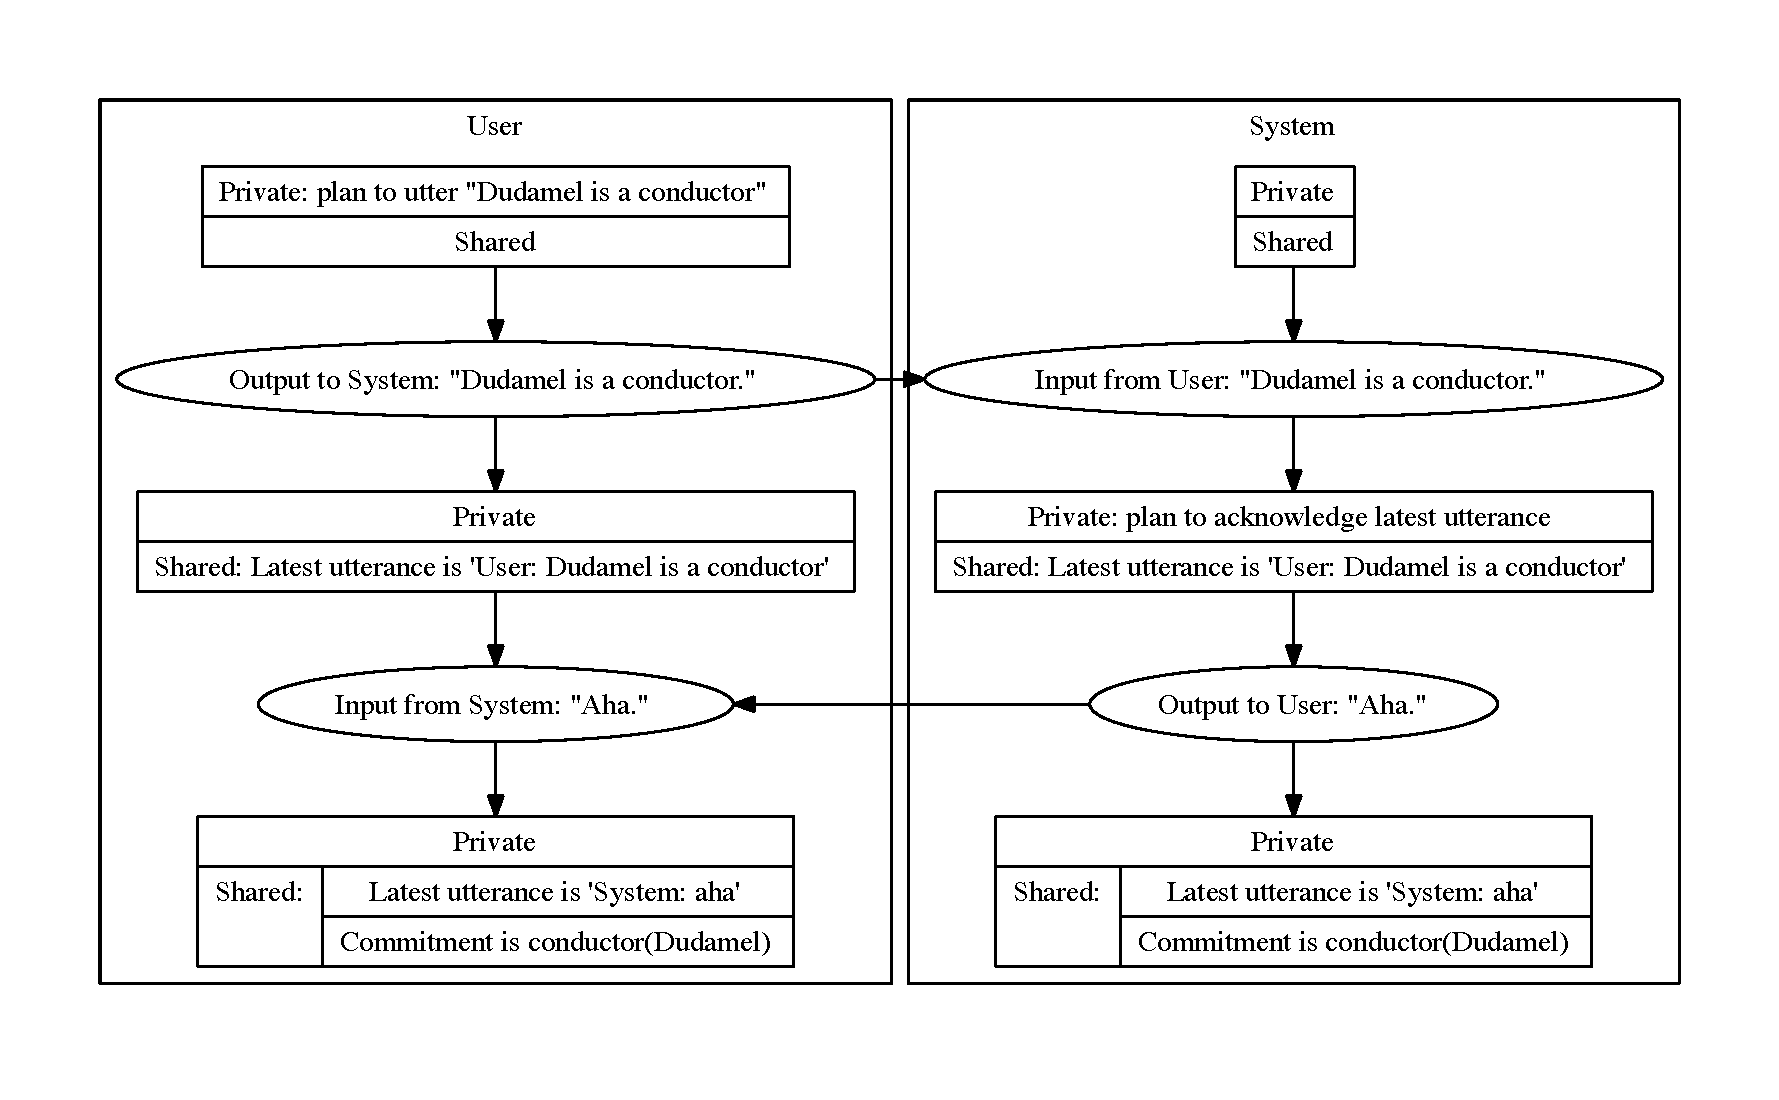
\includegraphics[width=\textheight]{simple-dm-diac}
\caption{Dialogue management:``Dudamel is a conductor''}
\label{fig:simple-dm-diac}
\end{sidewaysfigure}

%\clearpage

This assumes ideal
communication.  There is lots that could go wrong which could have the
consequence that the two agents become misaligned and an important
part of this framework is to provide a basis for the description of
miscommunication as well as communication.  (See
\cite{Ginzburg2012} for more discussion of this.)


We treat the dialogue information states represented by the square
boxes as records as in \nexteg{}.  


\begin{ex} 
\record{\field{private}{\record{\field{agenda}{\textit{AGENDA}}}} \\
        \field{shared}{\record{\field{latest-utterance}{\textit{L-UTT}} \\
                               \field{commitments}{\textit{COMM}}}}} 
\end{ex} 
  

What kinds of objects should \textit{AGENDA}, \textit{L-UTT} and
\textit{COMM} be?  % They will be defined with respect to the agent who
% owns the information state which, for convenience, we will refer to as
% \textit{SELF}.  We will see as we proceed with the discussion below
% that \textit{SELF} is related to the notion of \textit{de se} type act discussed in Section~\ref{sec:typeacts}.

We will say that \textit{AGENDA} is a list of sign \ignore{dialogue move} types,
that is,  the types of sign \ignore{dialogue moves} that the agent \ignore{\textit{SELF}} plans to
realize by means of a creation type act.  Recall from
Chapter~\ref{ch:percint} that this does not necessarily mean that
the agent \ignore{\textit{SELF}} is the main actor in the event
realizing the sign \ignore{move} type.
It can for example be a type of move to be carried out by an
interlocutor which the agent \ignore{\textit{SELF}} should wait for.  This will give us a
mechanism for handling basic turn-taking in dialogue.  (See
\citealp{SacksSchegloffJefferson1974} for the classic work on
turn-taking.) % We will define a dependent type \textit{Move} such that for any agent
% $A$, \textit{Move}($A$) is the type of dialogue moves in which $A$ is involved.
For now we will say that there are two ways in which an agent can be
involved in a dialogue act:  as speaker (or performer) or as hearer
(part of the audience to whom the dialogue act is
addressed).\footnote{A third way of being involved in a dialogue act
  which we will not take account of here is as an overhearer.}  % Performing a dialogue move is a \textit{de se} type act of creation as
% discussed in Chapter~\ref{sec:typeacts}.  Being the hearer or audience
% of a move type involves a \textit{de se} type act of judgement as
% discussed there.
% \textit{AGENDA}  should thus be a list of move types depending on
% \textit{SELF} (that
% is, subtypes of \textit{Move}(\textit{SELF})).  We introduce a
% dependent type,
% \textit{MoveType}, such that for any $a$:\textit{Ind},
% $T$:\textit{MoveType}($a$) iff $T\sqsubseteq\textit{Move}(a)$.
% \textit{AGENDA} is thus a list of move types and will
% have type [\textit{MoveType}(\textit{SELF})].   For any type $T$, $[T]$ is the type of
% lists all of whose members are of type $T$ (see
% Appendix~\ref{app:listtypes}).  We will come back to the details of
% \textit{Move} below.
% \todo{Move vs Sign?}

\textit{L-UTT} should tell us what the latest utterance in the
dialogue was.  This will be the witness of a sign type.  % move (or moves\footnote{See
%   \cite{Larsson2002} for a proposal where dialogue contributions
%   involve several moves. For now we will make the simplifying
%   assumption that utterances are associated with a single move.}) has just been carried out.
% But we will need more information than this.  We will need information about
% what (the agent \textit{SELF} thinks) was actually said.  For this we will use a
% chart, i.e. a set of edges between vertices representing hypotheses
% about parts of the utterance, that is, sign types associated with
% parts of the utterance.  The move should be predictable from the chart
% by a process of move-interpretation for which we will use the
% predicate `m-interp'.  Thus \textit{L-UTT} should itself be of
% the type \nexteg{}.

% \begin{ex} 
% \record{\tfield{move}{\textit{Move}(\textit{SELF})} \\
%         \tfield{chart}{\textit{Chart}} \\
%         \tfield{e}{m-interp(chart,move)}} 
% \end{ex} 
  

% The type \textit{Chart}
% we will say more about in Chapter~\ref{ch:gram}.

The commitments field has normally been considered as a set of
facts or propositions \citep{Ginzburg2012,Larsson2002}.  Here we will
treat them as a single record type, i.e. a witness of the type
\textit{RecType}.  Using a single type will make it more
straightforward to deal with issues like consistency and anaphora as
we will see in later chapters.

Thus information states can belong to the type \nexteg{}, our current
version of the type \textit{InfoState}.

\begin{ex} 
  \record{
    \tfield{private}{
      \record{
        \tfield{agenda}{$\mathrm{list}(\textit{RecType})$}}} \\
    \tfield{shared}{
      \record{
        \tfield{latest-utterance}{\textit{Sign}$^*$}\\
        \tfield{commitments}{\textit{RecType}}}}} 
\label{ex:InfoStatePrelim}
\end{ex}
Here \textit{Sign}$^*$ is the type of strings of signs of length 0 or
more using the string type notation introduced on
p.~\pageref{pg:stringtype-notation}.  At the beginning of a dialogue
there will be no latest utterance and we will represent this by having
the empty string of signs in `latest-utterance'-field.  By using
\textit{Sign}$^*$ we allow for the possibility that the previous
utterance can be represented by a string of several signs although in
the examples we will discuss here we will only have strings of length 1.

% (Here, by convention the labels `chart' and `move' in
% \smallrecord{\smalltfield{e}{m-interp(chart,move)}} refer to the path down to the minimal record in
% which the e-field occurs, that is `shared.latest-utterance.chart' and
% `shared.latest-utterance.move' respectively.)

% \preveg{} is, however, not quite general enough.  It requires that
% there always will be a latest utterance.  At the beginning of a
% dialogue this will not be the case and we need a way of representing
% that there is no previous utterance.  We will use a type whose only
% witness is the empty record for this.  Records, it will be recalled,
% are sets of ordered pairs (see
% Appendix~\ref{app:rectypes}).  This will include the empty set,
% $\emptyset$ which could also be notated as `[\ ]' if we are thinking
% of the empty set as the empty record.  However, this latter notation
% is confusing since it could also be used to represent the empty record
% type, that is the type that does not place any constraints on which
% records it has as witnesses, that is, the type of all records which we
% represent as \textit{Rec} in order to avoid confusion.  The type of
% the empty record could be constructed as the singleton type
% \textit{Rec}$_\emptyset$ (or if you are using the bracket notation for
% the empty record, \textit{Rec}$_{[\ ]}$).  In order to avoid
% notational confusion we will use \textit{ERec} to represent the type
% whose only witness is the empty record, that is, the empty set.  Thus
% \nexteg{} will hold.
% \begin{ex} 
% $a$ : \textit{ERec} iff $a=\emptyset$ 
% \end{ex} 
At the beginning of a
dialogue there will not be any shared commitments either.  Therefore, it
will be natural to use \textit{Rec} for the
commitments at the beginning of a dialogue.  \textit{Rec} is the type
of all records.  If we think of records as modelling situations then a
commitment represented by
\textit{Rec} is a commitment to the existence of a situation but not
to a situation of any particular type.  Thus it corresponds to ``there
is a situation'' or ``the world is not empty''.  It plays a similar
role in our theory to the set of all possible worlds in a system based
on possible worlds.  It represents a state where no constraints have
been placed on the nature of the world.   % The 
% adjustment we need to make to (\ref{ex:InfoStatePrelim}) in order to include dialogue
% initial information states is to the shared.latest-utterance field as
% in \nexteg{}.
% The `commitments'-field does not need to be adjusted as
The type \textit{Rec} is one of the witnesses of \textit{RecType} (see
Appendix~\ref{app:rectypes}).  The type of an initial information
state based on \preveg{} is \nexteg{}, that is, our current version of
the type \textit{InitInfoState}.
\begin{ex}
 \record{
    \tfield{private}{
      \record{
        \mfield{agenda}{[ ]}{$\mathrm{list}(\textit{RecType})$}}} \\
    \tfield{shared}{
      \record{
        \mfield{latest-utterance}{$\varepsilon$}{\textit{Sign}$^*$}\\
        \mfield{commitments}{\textit{Rec}}{\textit{RecType}}}}}   
% \smallrecord{\smalltfield{private}{\smallrecord{\smalltfield{agenda}{[\textit{MoveType}(\textit{SELF})]}}} \\
%         \smalltfield{shared}{\smallrecord{\smalltfield{latest-utterance}{\smallrecord{\smalltfield{move}{\textit{Move}(\textit{SELF})} \\
%                                                                   \smalltfield{chart}{\textit{Chart}}
%                                                                 \\
%                                                                   \smalltfield{e}{m-interp(chart,move)}}$\vee$\textit{ERec}}\\
%                                \smalltfield{commitments}{\textit{RecType}}}}}
% \label{ex:gameboard}
\end{ex}
% \preveg{} uses a join type (Appendix~\ref{app:jointypes}).  For any two
% types $T_1$ and $T_2$ you can form the join (or disjunction) $T_1\vee
% T_2$.  $a:T_1\vee T_2$ just in case either $a:T_1$ or $a:T_2$.

% \label{pg:SELF}We will use notation including `\textit{SELF}' as in \preveg{} to
% represent types which are derived from dependent types by applying
% them to the argument represented by \textit{SELF}.  This notational
% convention will save us a good deal of complication in presentation
% and it is always possible to recover the dependent type from which the
% type is derived by creating a function which maps an individual to the
% appropriate type.  Thus in the case of \preveg{} the dependent type
% would be \nexteg{}.
% \begin{ex}
% $\lambda a$:\textit{Ind} . \smallrecord{\smalltfield{private}{\smallrecord{\smalltfield{agenda}{[\textit{MoveType}($a$)]}}} \\
%         \smalltfield{shared}{\smallrecord{\smalltfield{latest-utterance}{\smallrecord{\smalltfield{move}{\textit{Move}($a$)} \\
%                                                                   \smalltfield{chart}{\textit{Chart}}
%                                                                 \\
%                                                                   \smalltfield{e}{m-interp(chart,move)}}$\vee$\textit{ERec}}\\
%                                \smalltfield{commitments}{\textit{RecType}}}}}
% \end{ex} 
% [???? This needs revising in order to include moves by agents other
% than \textit{SELF}!]

Some signs (but not all) will be associated with an \textit{illocutionary
force}, a term which originally comes from \cite{Austin1962}.  The four illocutionary forces we will consider here are:
assertion, query, command and acknowledgement.  Signs which have an
illocutionary force can be thought of as \textit{dialogue moves} or in
Austin's original terminology \textit{illocutionary acts}.
Those signs which are not associated with an illocutionary force are
normally constituents of something which does have illocutionary
force.  Thus, for example, if somebody says \textit{The dog barked}
the whole utterance can be thought of as an assertion.  However, the
utterance of \textit{the dog} which is part of this utterance does not
have illocutionary force.  This is not to say that some other
utterance of \textit{the dog} could not have illocutionary force.  For
example, in response to the question \textit{What made all the mess?},
an utterance of \textit{the dog} might be regarded as an assertion
that the dog made all the mess.

% Dialogue moves are a type of
% event in which an actor (normally speaker) is related to an intended
% audience, an illocutionary force (such as `assert') and a content
% (that is, for our present purposes, a record type such as \smallrecord{\smalltfield{e}{conductor(Dudamel)}}).

% , e.g. assert(User, System,
% conductor(Dudamel)).  We shall need to refine our view of what the
% third argument is.  But for now let us note that assert($a$,$b$,$c$)
% is a \textit{type}.  An object of this type will be an event or
% situation in which $a$ asserts $c$ with $b$ as the intended
% audience. ($b$ may or may not be able hear or comprehend $a$'s
% utterance.)  For technical reasons we will not use this type but one
% where the illocutionary force \textit{assert} is an argument:
% move(User, System, assert, conductor(Dudamel)).  We will need to access the various
% components of move types so that we can partially specify them.
% Therefore we will use the record type

% We will take dialogue moves to be a pairing of speech acts and content.
% The type of speech acts (\textit{SpeechAct}) will be taken to be a
% subtype of the type of speech events (\textit{SEvent}) as defined in
% (\ref{ex:SEventLocSpAu}) on p.~\pageref{ex:SEventLocSpAu}.  In
% particular this will mean that there is a field in a speech act for
% the speaker (labelled by `sp') and another for the audience (labelled
% by `au').  More
% specifically we will take the type \textit{Move}($a$) to be an abbreviation for
% \nexteg{}. 
% \begin{ex} 
% % \record{\tfield{actor}{\textit{Ind}} \\
% %         \tfield{audience}{\{\textit{Ind}\}} \\
% %         \tfield{orientation}{eq(\textit{SELF},actor)$\vee$member(\textit{SELF},audience)}
% %         \\
% %         \tfield{i-force}{\textit{IForce}} \\
% %         \tfield{content}{\textit{RecType}} \\
% %         \tfield{e}{move(actor, audience, i-force, content)}}
% \smallrecord{\smalltfield{e}{\textit{SpeechAct}}} $\wedge$ (
% \smallrecord{\smalltfield{e}{\smallrecord{\smallmfield{sp}{$a$}{\textit{Ind}}}}}
% $\vee$
% \smallrecord{\smalltfield{e}{\smallrecord{\smallmfield{au}{$a$}{\textit{Ind}}}}}
% )
% $\wedge$ \textit{MoveContent} 
% \label{ex:Move-a}
% \end{ex}
% The type in \preveg{} is a
% meet type (Appendix~\ref{app:meettypes}).\footnote{Strictly speaking, this type should be
%   written with parentheses since we are assuming a binary meet
%   operation:
%   (\smallrecord{\smalltfield{e}{\textit{SpeechAct}}} $\wedge$ ((
% \smallrecord{\smalltfield{e}{\smallrecord{\smallmfield{sp}{$a$}{\textit{Ind}}}}}
% $\vee$
% \smallrecord{\smalltfield{e}{\smallrecord{\smallmfield{au}{$a$}{\textit{Ind}}}}}
% )
% $\wedge$ \textit{MoveContent})) 
%   but we will often omit parentheses for clarity.} If $T_1$ and $T_2$ are
% types, then an object $a$ is of type  $T_1\wedge T_2$ just in case
% $a:T_1$ and $a:T_2$.  

% Note that \preveg{} requires $a$ to be either the speaker or the
% audience of the speech act and does not rule out the possibility that
% $a$ is both speaker and audience (i.e. $a$ is talking to herself).

% We
% will not attempt a complete inventory of speech act types here.
% Preliminarily, we could define \textit{SpeechAct} to be
% \begin{quote}
% \textit{Assertion}$\vee$\textit{Query}$\vee$\textit{Command}$\vee$\textit{Acknowledgement},
% \end{quote}
% that
% is, a join type (Appendix~\ref{app:jointypes}) of all the available
% speech act types.\footnote{Strictly speaking, this type should be
%   written with parentheses since we are assuming a binary join
%   operation:
%   (\textit{Assertion}$\vee$(\textit{Query}$\vee$(\textit{Command}$\vee$\textit{Acknowledgement})))
%   but we will often omit parentheses for clarity.}  Something will be of
% this type just in case it is of at least one of the types of the
% join.
% Each of the speech act types are subtypes of \textit{SEvent}
% and can be defined as in \nexteg{}.
We introduce four subtypes of \textit{Sign}:
\textit{Assertion}, \textit{Query}, \textit{Command} and
\textit{Acknowledgement}.  These are characterized in \nexteg{}. 
\begin{ex}
\begin{tabular}[t]{lcl}
\textit{Assertion} & -- & % \textit{SEvent} \d{$\wedge$} 
% \smallrecord{\smalltfield{e}{\textit{Phon}} \\
%              \smalltfield{c$_{\mathrm{illoc}}$}{assertion(e)}}
  \record{
  \tfield{s-event}{\textit{SEvent}}\\
  \tfield{cont}{\textit{RecType}}\\
  \tfield{illoc}{assert(s-event, cont)}
  }
  \\
\textit{Query} & -- & % \textit{SEvent} \d{$\wedge$} 
% \smallrecord{\smalltfield{e}{\textit{Phon}} \\
% \smalltfield{c$_{\mathrm{illoc}}$}{query(e)}}
  \record{
  \tfield{s-event}{\textit{SEvent}}\\
  \tfield{cont}{\textit{Question}}\\
  \tfield{illoc}{query(s-event, cont)}
  }
  \\
\textit{Command} & -- & % \textit{SEvent} \d{$\wedge$} 
% \smallrecord{\smalltfield{e}{\textit{Phon}} \\
% \smalltfield{c$_{\mathrm{illoc}}$}{command(e)}}
  \record{
  \tfield{s-event}{\textit{SEvent}}\\
  \tfield{cont}{\textit{RecType}}\\
  \tfield{illoc}{command(s-event, cont)}
  }
  \\
\textit{Acknowledgement} & -- & % \textit{SEvent} \d{$\wedge$} 
% \smallrecord{\smalltfield{e}{\textit{Phon}} \\
% \smalltfield{c$_{\mathrm{illoc}}$}{acknowledgement(e)}}
  \record{
  \tfield{s-event}{\textit{SEvent}}\\
  \tfield{cont}{\textit{RecType}}\\
  \tfield{illoc}{acknowledge(s-event, cont)}
  }
  

\end{tabular} 
\end{ex}
Note that the type of the content varies with the illocutionary
force.  We use the type \textit{Question} for queries and
\textit{RecType} for the others.  We will say more about
\textit{Question} in later chapters.  It is quite likely that the
content type for commands should be something other than
\textit{RecType}, for example, the type \textit{Ppty} (``property'')
that we will develop in later chapters, but we do not have more to say
about commands in this work.  In a more complete treatment of
illocutionary force the nature of the speech event could also be made
to vary with illocutionary force.  For example, we could require
question syntax for queries, although that would not take account of
the fact that declarative sentence syntax can also be used to ask
questions.  It is not our aim here to give a detailed analysis of such
phenomena but to provide a general framework in which they could be
analyzed.

We will also introduce types \textit{AssertionType},
\textit{QueryType}, \textit{CommandType} and
\textit{AcknowledgementType} which are characterized in a similar way
to \textit{SignType} as in \nexteg{}.
\begin{ex} 
\begin{subex} 
 
\item $T:\textit{AssertionType}$ iff $T\sqsubseteq \textit{Assertion}$ 
 
\item $T:\textit{QueryType}$ iff $T\sqsubseteq \textit{Query}$

  
\item $T:\textit{CommandType}$ iff $T\sqsubseteq \textit{Command}$

  
\item $T:\textit{AcknowledgementType}$ iff $T\sqsubseteq \textit{Acknowledgement}$ 
 
\end{subex} 
   
\end{ex} 
  

% Here the subscript `illoc' stands for ``illocutionary'' indicating
% that the condition provides information about the illocutionary force
% of the speech act. The symbol \d{$\wedge$} represents the merge operation defined in
% Appendix~\ref{app:merge}.  In \preveg{} the relevant merges will be
% the unions of the sets of fields represented by \textit{SEvent} and
% the type consisting of the `e' and `illoc' fields.  This is
% illustrated in \nexteg{} for \textit{Assertion}. \nexteg{a} (where
% \textit{SEvent} is spelled out) is
% identical with \nexteg{b}.
% \begin{ex} 
% \begin{subex} 
 
% \item \record{\tfield{e-loc}{\textit{Loc}} \\
%         \tfield{sp}{\textit{Ind}} \\
%         \tfield{au}{\textit{Ind}} \\
%         \tfield{e}{\textit{Phon}} \\
%         \tfield{c$_{\mathrm{loc}}$}{loc(e,e-loc)} \\
%         \tfield{c$_{\mathrm{sp}}$}{speaker(e,sp)} \\
%         \tfield{c$_{\mathrm{au}}$}{audience(e,au)}} \d{$\wedge$} 
% \smallrecord{\smalltfield{e}{\textit{Phon}} \\
%              \smalltfield{c$_{\mathrm{illoc}}$}{assertion(e)}}
 
% \item \record{\tfield{e-loc}{\textit{Loc}} \\
%         \tfield{sp}{\textit{Ind}} \\
%         \tfield{au}{\textit{Ind}} \\
%         \tfield{e}{\textit{Phon}} \\
%         \tfield{c$_{\mathrm{loc}}$}{loc(e,e-loc)} \\
%         \tfield{c$_{\mathrm{sp}}$}{speaker(e,sp)} \\
%         \tfield{c$_{\mathrm{au}}$}{audience(e,au)} \\
%         \tfield{c$_{\mathrm{illoc}}$}{assertion(e)}}

 
% \end{subex} 
   
% \end{ex} 
  

% Finally, the type \textit{MoveContent} in (\ref{ex:Move-a}) relates the type
% of the content of the move to the type of the move.  We define it
% preliminarily as the join type in \nexteg{}.
% \begin{ex} 
% \record{\tfield{e}{\textit{Assertion}} \\
%         \tfield{cont}{\textit{RecType}} \\
%         \tfield{c$_{\mathrm{cont}}$}{content(e,cont)}}$\vee$
% \record{\tfield{e}{\textit{Query}} \\
%         \tfield{cont}{\textit{Question}} \\
%         \tfield{c$_{\mathrm{cont}}$}{content(e,cont)}}$\vee$
% \record{\tfield{e}{\textit{Command}} \\
%         \tfield{cont}{\textit{RecType}} \\
%         \tfield{c$_{\mathrm{cont}}$}{content(e,cont)}}$\vee$
% \record{\tfield{e}{\textit{Acknowledgement}}} 
% \end{ex} 
% Note that this allows for acknowledgements such as \textit{ok} not to
% have any content (although it does not prevent them from having content).  We will return later to discussion of whether this
% is a reasonable claim for acknolwedgements, while noting that this would  be one way of
% dealing with ``phatic'' communication such as greetings like \textit{Hello}.

% We place a condition on `self' that it be the ``ego'', that is, that
% it involves a situation which is of the type ego(self).  The idea is
% that this is a type \textit{de se} by which we mean that a judgement
% that a situation $s$ is of the type ego($a$) requires that $a$ is the
% individual making the judgement.  We do not have a formal treatment of
% this.  We have relativized our judgements in Appendix~\ref{app:ttr} to
% systems of types involving assignments to the basic types but not to
% the agent making the judgement.  We will not develop this further here
% but merely note that the perception of oneself as the actor or the
% audience of a dialogue move is an essentially \textit{de se}
% phenomenon. For recent discussion of and a survey of the literature on
% \textit{de se} phenomena see \cite{Ninan2010,Hanks2012}.
  

% We will be able to read partial information about
% a dialogue move from certain aspects of a speech-event.  For example,
% an utterance of \textit{ok}
% may tell us that the dialogue move is of type \nexteg{}.

% \begin{ex} 
% % \record{\tfield{actor}{\textit{Ind}} \\
% %         \tfield{audience}{\{\textit{Ind}\}} \\
% %         \tfield{orientation}{member(\textit{SELF},audience)} \\
% %         \mfield{i-force}{acknowledge}{\textit{IForce}} \\
% %         \tfield{content}{\textit{RecType}} \\
% %         \tfield{e}{move(actor, audience, i-force, content)}} 
% \record{\tfield{e}{\textit{Acknowledgement}} \\
%         \mfield{sp}{\textit{SELF}}{\textit{Ind}}}
% \end{ex} 
In order to find the content of an utterance of \textit{ok}, we look
to the content of the previous utterance.  Thus an utterance of
\textit{ok} following an utterance of \textit{Dudamel is a conductor}
will have the same content as the assertion,  namely \nexteg{}.
\begin{ex} 
\record{\tfield{e}{conductor(dudamel)}} 
\end{ex} 
Assigning \preveg{} as the content of \textit{Dudamel is a conductor}
involves the naive assumption that a proper name uniquely identifies a
particular individual.  We will develop a more sophisticated approach
to proper names in Chapters~\ref{ch:gram} and \ref{ch:propnames}.  
% An
% utterance of \textit{Dudamel is a conductor} may give us information
% about the type of speech act (\textit{Assertion}) and the content
% (\smallrecord{\smalltfield{e}{conductor(Dudamel)}}).  Note, however,
% that we only get such a fully specified content if we have a unique
% individual `Dudamel' whom we associate with utterances of the name
% \textit{Dudamel}.  If the resources we have available do not give us
% such an individual associated with \textit{Dudamel} then we only get
% the information that somebody named Dudamel is a conductor, that is,
% we may only get partial information about the content the speaker
% intended to communicate.  Consider the example \textit{Strauss is a
%   composer}.  There are at least two famous composers named Strauss
% (and also some more not so famous ones).  If our available resources
% give us two people associated with the name \textit{Strauss} we will
% not know which of them is being referred to.  Representing contents as record types will 
% enable us to handle this content underspecification. However, in order
% to do this we will need to abandon our current simplifying
% ``propositional logic'' assumption
% that sentences come as unanalyzed wholes associated with their
% contents.  This we will do in Chapter~\ref{ch:gram}.
% We will talk
% about the exact nature of the record type when we talk about semantics below.


% Not surprisingly, when we are dealing with an agenda as in (\ref{ex:gameboard}), a
% plan for future action, we have got ourselves into a situation
% where we need types rather than the objects.  The things that are on
% the agenda list are not actual events, but rather \textit{types} of
% events planned for the future.  Normally the types occurring on the
% agenda will be subtypes of \textit{Move}(\textit{SELF}), though we may wish to
% include types of events like looking something up in a database,
% i.e. non-speech events.

% For the most part types on the agenda will not be completely specified
% types.  That is they will not be types all of whose fields are
% manifest (restricted to particular objects of those types).
% Frequently it will be the case that we specify the content of the move
% but leave open the phonology, that is, the type will specify the
% content of what is to be said but not actually what is to be said or
% even perhaps which language it should.  We want, for example, to be able to
% say that a speaker is carrying out the same type of move independently of which
% language they are speaking.  Thus, if the user says to the system ``Dudamel is a conductor''
% or (in Swedish) ``Dudamel �r dirigent'' she will in both cases have carried out a
% move involving the assertion of the content \smallrecord{\smalltfield{e}{conductor(Dudamel)}}.  This abstraction will
% be important, for example, if we want to change language in the middle
% of a dialogue, as people sometimes do.\footnote{This phenomenon is
%   known as code-switching \citep{BullockToribio2009}.}  At the same time it is the
% normal case to continue a dialogue in the same language and thus we
% need to note which language was used in the previous utterance,
% i.e. keep track of what was actually said.  This information will be
% in the chart which is part of the latest move.  In the chart there
% will be
% more information about what was actually said which will be important when it comes to dealing
% with parts of the utterance for things like clarification and
% anaphora.  But this again requires us to abandon our current
% simplifying ``propositional logic'' assumption.
    

% We will assume that agents do not have complete
% information about the information state, that is, they reason in terms
% of \textit{types} of information state (that is, gameboards).
% The basic intuition behind our reasoning about information state
% updates can be expressed as in \nexteg{}.

% \begin{ex} 
% If $r_i$ : $T_i$, then $r_{i+1}$ : $T_{i+1}(r_i)$ 
% \end{ex} 
  

% That is, given that we believe that the current information state is
% of type $T_i$ (recall that we can come to this belief without having
% any belief about which specific information state is involved), then
% we can conclude that the next information state is of type $T_{i+1}$
% which can depend on the current information state.  According to this,
% we can have a hypothesis about the type of the next information state
% even though we may not know exactly what the current information state
% is.  Exactly which type the next information state belongs to depends,
% though, on the exact nature of the current information state.  Thus
% the dependency in our types provides us with an additional means for
% representing underspecification.

% This basic rule of inference corresponds to a function from records to
% record types, a function of type ($T_i$ $\rightarrow$ {\it
%   RecType\/}), that is, one kind of update function we were using in Chapter~\ref{ch:percint}.  Such a function is of
% the form \nexteg{}. 

% \begin{ex} 
% $\lambda r\!:\!T_i\ .\ T_{i+1}(r)$ 
% \end{ex} 
  

% Things are a litte more complicated than this, however, because this
% only represents the change from one information state to another,
% whereas in fact this change is triggered by a speech
% event which bears an appropriate relation to the current information
% state represented by $r$.  Thus we are actually interested in
% functions from the current information state to a function from events
% to the new information state, as in \nexteg{}.

% \begin{ex}
% $\lambda r\!:\!T_i\ .\ \lambda e\!:\!T_e(r)\ .\ T_{i+1}(r,e)$
% \label{eg:updateFun}
% \end{ex}

% This is the other kind of update function we were using in Chapter~\ref{ch:percint}.\footnote{This is
%   one of a number of ways of characterizing update in this kind of
%   framework.  One might for instance think of the type of the speech event as
%   being part of the current information state.  Also instead of using
%   an update function one can use a record type with a
%   `preconditions'-field and an `effect'-field.  Both
%   \cite{Ginzburg2012} and \cite{Larsson2002} have this kind of approach.}
Let us consider
the update function and update rule which the user could use in order to update her
information state after her own utterance of \textit{Dudamel is
  a conductor}.  This is modelled on the kind of integration rules
discussed in \cite{Larsson2002}.  The update function we wish to
characterize will be defined on information states which have some
assertion type as the first element on the agenda, that is the type in
\nexteg{}.
\begin{ex} 
\record{
    \tfield{private}{
      \record{
        \tfield{agenda}{
          \record{
            \tfield{fst}{\textit{AssertionType}}\\
            \tfield{rst}{$\mathrm{list}(\textit{RecType})$}}}}} \\
    \tfield{shared}{
      \record{
        \tfield{latest-utterance}{\textit{Sign}$^*$}\\
        \tfield{commitments}{\textit{RecType}}}}}  
\end{ex} 
Rather than writing out such types in our update functions we can
think of the objects in the domain of our update
function as meeting the requirement that they belong to two types as
in \nexteg{}.
\begin{ex} 
\begin{subex} 
 
\item \textit{InfoState} 
 
\item
  \record{
    \tfield{private}{
      \record{
        \tfield{agenda}{
          \record{
            \tfield{fst}{\textit{AssertionType}}}}}}}
 
\end{subex} 
   
\end{ex} 
A statement of the update function in terms of the abbreviation
\textit{InfoState} will not only save space but also be helpful as we
further develop our notion of what type \textit{InfoState} represents.
If we are just adding extra fields to the type \textit{InfoState},
that is we develop our theory monotonically just by adding more
detail, then we do not have to go back and revise the formulation of
the update functions based on earlier versions of the theory.

However, we still need to give a characterization of a single type
which will serve as the domain type of the update function.  One way
to do this is to use TTR's \textit{meet types} such as \nexteg{}.
\begin{ex} 
  (\textit{InfoState} $\wedge$
  \record{
    \tfield{private}{
      \record{
        \tfield{agenda}{
          \record{
            \tfield{fst}{\textit{AssertionType}}}}}}}) 
\end{ex} 
In general $a:(T_1\wedge T_2)$ just in case $a:T_1$ and $a:T_2$.

\begin{shaded}
We can introduce meet (also known as intersection or conjunctive
types) into a type system as in \nexteg{}, repeated in
Appendix~\ref{app:meettypes}.
\begin{ex} 
A system of complex types \textbf{TYPE}$_C$ = $\langle${\bf Type}, {\bf BType},
$\langle$\textbf{PType}, {\bf Pred}, \textbf{ArgIndices}, {\it
  Arity\/}$\rangle$, $\langle A,F\rangle$$\rangle$ \textit{has meet types} if
\begin{enumerate} 
 
\item for any $T_1,T_2 \in \mathbf{Type}$, $(T_1\wedge T_2) \in \mathbf{Type}$ 
 
\item for any $T_1,T_2 \in \mathbf{Type}$, $a:_{\mathbf{TYPE_C}}(T_1\wedge T_2)$ iff
  $a:_{\mathbf{TYPE_C}}T_1$ and $a:_{\mathbf{TYPE_C}}T_2$ 

\end{enumerate}
\label{ex:meettypes}
\end{ex} 
In our informal proof theoretic notation this can be represented as
\nexteg{}.
\begin{ex} 
  For $\Gamma$ a system of complex types
  \begin{subex} 
 
  \item
    \begin{prooftree}
      \hypo{\Gamma\vdash T_1\in\textbf{Type}}
      \hypo{\Gamma\vdash T_2\in\textbf{Type}}
      \infer2{\Gamma\vdash (T_1\wedge T_2)\in\textbf{Type}}
    \end{prooftree}
    
 
  \item
    \begin{prooftree}
      \hypo{\Gamma\vdash a:T_1}
      \hypo{\Gamma\vdash a:T_2}
      \infer2{\Gamma\vdash a:(T_1\wedge T_2)}
    \end{prooftree}

    
  \item
    \begin{prooftree}
      \hypo{\Gamma\vdash a:(T_1\wedge T_2)}
      \infer1{\Gamma\vdash a:T_1}
    \end{prooftree}

    
  \item
    \begin{prooftree}
      \hypo{\Gamma\vdash a:(T_1\wedge T_2)}
      \infer1{\Gamma\vdash a:T_2}
    \end{prooftree}
 
\end{subex} 
  
\end{ex} 
Just as we did for join types we can introduce a generalized version
of meet types as in \nexteg{}, repeated in Appendix~\ref{app:meettypes}.
\begin{ex} 
A system of complex types {\bf TYPE$_C$} = $\langle${\bf Type}, {\bf BType},
$\langle$\textbf{PType}, {\bf Pred}, \textbf{ArgIndices}, {\it
  Arity\/}$\rangle$, $\langle A,F\rangle$$\rangle$ \textit{has
  generalized meet
  types} if 

\begin{enumerate} 
 
\item for any non-empty finite set of types, $\mathbb{T}$, such that $\mathbb{T}
  \subseteq\mathbf{Type}$, $\bigwedge\mathbb{T} \in \mathbf{Type}$ 
 
\item for any finite $\mathbb{T} \subseteq\mathbf{Type}$, $a:_{\mathbf{TYPE_C}}\bigwedge\mathbb{T}$ iff
  $a:_{\mathbf{TYPE_C}}T$ for all $T\in\mathbb{T}$
 
\end{enumerate}
\label{ex:genmeettypes}
\end{ex} 
In our informal proof theoretic notation this can be represented as
\nexteg{}.
\begin{ex} 
  For $\Gamma$ a system of complex types
  \begin{subex} 
 
  \item
    \begin{prooftree}
      \hypo{\Gamma\vdash T_1,\ldots,T_n\in\textbf{Type}}
      \infer1{\Gamma\vdash\bigwedge\{T_1,\ldots,T_n\}\in\textbf{Type}}
    \end{prooftree}
    
 
  \item
    \begin{prooftree}
      \hypo{\Gamma\vdash a:T_1,\ldots,a:T_n}
      \infer1{\Gamma\vdash a:\bigwedge\{T_1,\ldots,T_n\}}
    \end{prooftree}

    
  \item
    \begin{prooftree}
      \hypo{\Gamma\vdash a:\bigwedge\{T_1,\ldots,T_n\}}
      \hypo{1\leq i\leq n}
      \infer2{\Gamma\vdash a:T_i}
    \end{prooftree}
    
 
\end{subex} 
  
\end{ex}
As with join types, we can, if we wish, use $T_1\wedge\ldots\wedge
T_n$ to represent $\bigwedge\{T_1,\ldots,T_n\}$.
  
\end{shaded}

If $T_1$ and $T_2$ are record types then there will always be a record
type (not a meet) 
$T_3$ which is necessarily equivalent to $T_1\wedge T_2$, that is any
record, $r$ of type $T_1\wedge T_2$ will be of type $T_3$ and
\textit{vice versa}.  We will call this the \textit{merge} of $T_1$
and $T_2$ which we will represent as $T_1$\d{$\wedge$}$T_2$ (with a dot
under `$\wedge$').  For example, \nexteg{a} will have the same set
of witnesses as \nexteg{b}.
\begin{ex} 
\begin{subex} 
 
\item  \record{\tfield{f}{$T_1$}}$\wedge$\record{\tfield{g}{$T_2$}}
 
\item \record{\tfield{f}{$T_1$}\\
        \tfield{g}{$T_2$}} 
 
\end{subex} 
   
\end{ex} 
When a label only occurs in one of the types being merged then the
field with that label is also a field of the merge of the two types.
Thus \nexteg{} holds.
\begin{ex} 
\record{\tfield{f}{$T_1$}}\d{$\wedge$}\record{\tfield{g}{$T_2$}} = \record{\tfield{f}{$T_1$}\\
        \tfield{g}{$T_2$}} 
\end{ex} 
When the same label, $\ell$, occurs in both types, then whatever
occurs in the $\ell$-field must be of the types required in those
fields by both the types.  Thus \nexteg{a} and \nexteg{b} will have
the same witnesses.
\begin{ex} 
\begin{subex} 
 
\item \record{\tfield{f}{$T_1$}}$\wedge$\record{\tfield{f}{$T_2$}} 
 
\item \record{\tfield{f}{$T_1\wedge T_2$}} 
 
\end{subex} 
   
\end{ex} 
In a case like this we will make the merge recursive down inside the
type, that is, we will make merge the types in the `f'-field in
\preveg{b}.  Thus \nexteg{} will hold.
\begin{ex} 
  \record{\tfield{f}{$T_1$}}\d{$\wedge$}\record{\tfield{f}{$T_2$}} =
  \record{\tfield{f}{$T_1$\d{$\wedge$}$T_2$}}
\end{ex} 
If one or the other of $T_1$ and $T_2$ is not a record type then
$T_1$\d{$\wedge$}$T_2$ will be $T_1\wedge T_2$.  If $T_1\sqsubseteq T_2$
then $T_1$\d{$\wedge$}$T_2$ is $T_1$ and if $T_2\sqsubseteq T_1$
then $T_1$\d{$\wedge$}$T_2$ is $T_2$.  

\begin{shaded}
We can define the merge operation on types in the following way
(repeated in Appendix~\ref{app:merge}).\label{pg:merge} The definition
is closely related to the unification algorithms used in feature based
grammar (see \citealp{Shieber1986} for the classic reference).

We define a function $\mu$ which maps meets of record types to an
equivalent record type, record types to equivalent types where meets
in their values have been simplified by $\mu$ and any other types to
themselves:
\begin{enumerate}
  \item if for some $T_1,T_2$, $T=(T_1\wedge T_2)$ and $T_1\sqsubseteq T_2$
  then $\mu(T)=T_1$ 
 
\item if for some $T_1,T_2$, $T=(T_1\wedge T_2)$ and $T_2\sqsubseteq T_1$
  then $\mu(T)=T_2$
  
\item otherwise:
\begin{enumerate} 
 
\item if for some $T_1$, $T_2$, $T=(T_1\wedge T_2)$ then
  $\mu(T)=\mu'(\mu(T_1)\wedge\mu(T_2))$. 
 
\item if $T$ is a record type then $\mu(T)$ is $T'$ such that for any
  $\ell$,$v$, $\langle\ell,\mu(v)\rangle\in T'$ iff
  $\langle\ell,v\rangle\in T$.

\item otherwise $\mu(T)=T$.
 
\end{enumerate}
\end{enumerate}

$\mu'(T_1\wedge T_2)$ is defined by:
\begin{enumerate} 
 
\item if $T_1$ and $T_2$ are record types, then $\mu'(T_1\wedge
  T_2)=T_3$ such that
\begin{enumerate} 
 
\item for any $\ell,v_1,v_2$, if $\langle\ell,v_1\rangle\in T_1$ and
  $\langle\ell,v_2\rangle\in T_2$, then 

\begin{enumerate} 
 
\item if $v_1$ and $v_2$ are
\begin{quote}
  $\langle\lambda u_1\!\!:\!\!T'_1\ldots\lambda
  u_i\!\!:\!\!T'_i\ .\ \phi,\langle\pi_1\ldots\pi_i\rangle\rangle$
  \end{quote}
  and
  \begin{quote}
    $\langle\lambda u'_1\!\!:\!\!T''_1\ldots\lambda
  u'_k\!\!:\!\!T''_k\ .\ \psi,\langle\pi'_1\ldots\pi'_k\rangle\rangle$
\end{quote}
respectively, then
\begin{quote}
$\langle\lambda u_1\!\!:\!\!T'_1\ldots\lambda
  u_i\!\!:\!\!T'_i,\lambda u'_1\!\!:\!\!T''_1\ldots\lambda
  u'_k\!\!:\!\!T''_k\ .\ \mu(\phi\wedge\psi), \langle\pi_1\ldots\pi_i,\pi'_1\ldots\pi'_k\rangle\rangle\in T_3$
\end{quote}

\item if $v_1$ is
  \begin{quote}
$\langle\lambda u_1\!\!:\!\!T'_1\ldots\lambda
u_i\!\!:\!\!T'_i\ .\ \phi,\langle\pi_1\ldots\pi_i\rangle\rangle$
\end{quote}
and $v_2$ is a
  type (i.e. not of the form $\langle f,\Pi\rangle$ for some function
  $f$ and sequence of paths $\Pi$), then
  \begin{quote}
    $\langle\lambda u_1\!\!:\!\!T'_1\ldots\lambda
  u_i\!\!:\!\!T'_i\ .\ \mu(\phi\wedge
  v_2),\langle\pi_1\ldots\pi_i\rangle\rangle\in T_3$
\end{quote}

\item if $v_2$ is
  \begin{quote}
    $\langle\lambda u'_1\!\!:\!\!T''_1\ldots\lambda
  u'_k\!\!:\!\!T''_k\ .\
  \psi),\langle\pi'_1\ldots\pi'_k\rangle\rangle$
\end{quote}
and $v_1$
is a type, then
\begin{quote}
  $\langle\lambda u'_1\!\!:\!\!T''_1\ldots\lambda
  u'_k\!\!:\!\!T''_k\ .\ \mu(v_1\wedge\psi)),\langle\pi'_1\ldots\pi'_k\rangle\rangle\in
  T_3$
  \end{quote}

\item otherwise $\langle\ell,\mu(v_1\wedge
  v_2)\rangle\in T_3$ 
 
\end{enumerate} 
  


 
\item for any $\ell,v_1$, if $\langle\ell,v_1\rangle\in T_1$ and there
  is no $v_2$ such that $\langle\ell,v_2\rangle\in T_2$, then
  $\langle\ell,v_1\rangle\in T_3$

\item for any $\ell,v_2$, if $\langle\ell,v_2\rangle\in T_2$ and there
  is no $v_1$ such that $\langle\ell,v_1\rangle\in T_1$, then
  $\langle\ell,v_2\rangle\in T_3$
 
\end{enumerate} 

% \item if $T_1$ and $T_2$ are record types and $T_2\sqsubseteq T_1$, then
%   $\mu'(T_1\wedge T_2)=T_2$

% \item if $T_1$ and $T_2$ are record types and $T_1\sqsubseteq T_2$, then
%   $\mu'(T_1\wedge T_2)=T_1$

\item if $T_1$ is $\mathrm{list}(T_1')$ ($\mathrm{set}(T_1')$, $\mathrm{plurality}(T_1')$) and
  $T_2$ is $\mathrm{list}(T_2')$ ($\mathrm{set}(T_2')$, $\mathrm{plurality}( T_2')$), then
  $\mu'(T_1\wedge T_2)=\mathrm{list}(\mu(T_1'\wedge T_2'))$ ($\mathrm{set}(\mu(T_1'\wedge
  T_2'))$, $\mathrm{plurality}(\mu(T_1'\wedge T_2'))$)
   
 
\item \label{item:mergeotherwise} otherwise $\mu'(T_1\wedge T_2)=T_1\wedge T_2$ 
 
\end{enumerate} 

$(T_1$ \d{$\wedge$} $T_2)$ is used to represent $\mu(T_1\wedge T_2)$.
We call  $(T_1$ \d{$\wedge$} $T_2)$ the \textit{merge} of $T_1$ and
$T_2$.

It is important for this characterization of merge to work properly
that paths in record types extend into meet types within the record
type.  Consider the merge expressed in \nexteg{a} where we assume that
\textit{Sit} is a basic type, for example the type of situations.
According to the above definition \nexteg{a} will be identical with
\nexteg{b}.
\begin{ex} 
\begin{subex} 
 
\item \record{
    \tfield{e}{\record{
        \tfield{x}{\textit{Ind}}\\
        \tfield{y}{\textit{Ind}}\\
        \tfield{e}{hug(x,y)}}} \\
    \tfield{c$_1$}{boy(e.x)}\\
    \tfield{c$_2$}{dog(e.y)} 
  } \d{$\wedge$} \record{\tfield{e}{\textit{Sit}}} 
 
\item \record{
    \tfield{e}{\record{
        \tfield{x}{\textit{Ind}}\\
        \tfield{y}{\textit{Ind}}\\
        \tfield{e}{hug(x,y)}} $\wedge$ \textit{Sit}} \\
    \tfield{c$_1$}{boy(e.x)}\\
    \tfield{c$_2$}{dog(e.y)} 
  } 
 
\end{subex} 
\label{ex:paths-into-meets}   
\end{ex} 
If the paths of record types do not extend into meet types then the
paths of \preveg{b} would be \nexteg{} and \preveg{} would not be a
well-formed record type since the `c$_1$' and `c$_2$'-fields would
reference non-existant paths.
\begin{ex} 
\{e, c$_1$, c$_2$\} 
\end{ex} 
However, clearly any record which is of the type (\ref{ex:paths-into-meets}b)  must in addition
have the paths `e.x' and `e.y' because of the requirement expressed by
the meet type.  Thus it is appropriate and intuitive that these should
count as paths in the record type thus making
(\ref{ex:paths-into-meets}b) well-formed.  


\end{shaded}

In our update action rules we will make use of an operation called
\textit{asymmetric merge}.\label{pg:asymmerge}  The asymmetric merge of types $T_1$ and
$T_2$, $T_1$\fbox{\d{$\wedge$}}$T_2$ is like their merge except that
if either $T_1$ or $T_2$ is not a record type then
$T_1$\fbox{\d{$\wedge$}}$T_2$ is $T_2$.  Also asymmetric merge does
not check for subtyping in the way that ordinary merge does.  Thus
when asymmetrically merging non-record types, $T_1$ and $T_2$,
$T_1$\fbox{\d{$\wedge$}}$T_2$ will always be $T_2$ regardless of
whether the subtype relation holds between the two types.

\begin{shaded}
We can define asymmetric merge in the following way (repeated in
Appendix~\ref{app:merge}).  The definition is closely related to the
priority unification algorithms used in feature based grammar
\citep{Shieber1986}.

The \textit{asymmetric merge} of $T_1$ and
$T_2$ is defined by a function, $\mu_{\mathrm{asym}}$, exactly
like $\mu$ except that the first two clauses of the definition of
$\mu$ are missing and $\mu'$ is replaced by another function
$\mu_{\mathrm{asym}}'$.  Thus the definition of $\mu_{\mathrm{asym}}$
is:
\begin{enumerate} 
 
\item if for some $T_1$, $T_2$, $T=(T_1\wedge T_2)$ then
  $\mu_{\mathrm{asym}}(T)=\mu_{\mathrm{asym}}'(\mu_{\mathrm{asym}}(T_1)\wedge\mu_{\mathrm{asym}}(T_2))$. 
 
\item if $T$ is a record type then $\mu_{\mathrm{asym}}(T)$ is $T'$ such that for any
  $\ell$,$v$, $\langle\ell,\mu_{\mathrm{asym}}(v)\rangle\in T'$ iff
  $\langle\ell,v\rangle\in T$.

\item otherwise $\mu_{\mathrm{asym}}(T)=T$.
 
\end{enumerate}

The definition of $\mu_{\mathrm{asym}}'$ is exactly like $\mu'$,
replacing $\mu$ and $\mu'$ with $\mu_{\mathrm{asym}}$ and $\mu_{\mathrm{asym}}'$ respectively, except that
the
clause~\ref{item:mergeotherwise} of the definition of $\mu'$ is replaced by 
\begin{enumerate} 
 
\item[\ref{item:mergeotherwise}$'$.] otherwise $\mu_{\mathrm{asym}}'(T_1\wedge T_2)=T_2$ 
 
\end{enumerate} 
  
We use $T_1$ \fbox{\d{$\wedge$}} $T_2$  to represent the asymmetric
merge of $T_1$ and $T_2$.  

Asymmetric merge may result in an ill-formed record type if we take
the asymmetric merge of a record type, $T_1$, and a non-record type,
$T_2$, since $T_1$ may be embedded in a larger type with fields
dependent on paths into $T_1$ which will not be present in the result
where $T_2$ has been substituted for $T_1$ thus removing the relevant
paths.  Consider the asymmetric merge \nexteg{a} which is \nexteg{b},
where, as above, \textit{Sit} is a basic type.
\begin{ex} 
\begin{subex} 
 
\item \record{
    \tfield{e}{\record{
        \tfield{x}{\textit{Ind}}\\
        \tfield{y}{\textit{Ind}}\\
        \tfield{e}{hug(x,y)}}} \\
    \tfield{c$_1$}{boy(e.x)}\\
    \tfield{c$_2$}{dog(e.y)} 
  } \fbox{\d{$\wedge$}} \record{\tfield{e}{\textit{Sit}}} 
 
\item \record{
    \tfield{e}{\textit{Sit}} \\
    \tfield{c$_1$}{boy(e.x)}\\
    \tfield{c$_2$}{dog(e.y)} 
  } 
 
\end{subex} 

\end{ex} 
\preveg{b} is clearly not a well-formed type since the fields labelled
by `c$_1$' and `c$_2$' address non-existent paths.

\end{shaded}

Armed with this technology we can define an update function,
f$_{\textsc{PlanAccAss}}$,  and action
rule which plan an acknowledgement to an assertion as in \nexteg{}.
\begin{ex} 
\begin{subex} 
 
\item f$_{\textsc{PlanAckAss}}$

  $\lambda r$:\textit{InfoState} . \\
  \hspace*{2em}$\lambda u$:\textit{Assertion} . \\
  \hspace*{4em}
  \smallrecord{
    \smalltfield{private}{\smallrecord{
        \smalltfield{agenda}{\smallrecord{
            \smalltfield{fst}{\smallrecord{
                \smalltfield{s-event}{\textit{SEvent} \d{$\wedge$} \smallrecord{
                    \smallmfield{sp}{$u$.s-event.au}{\textit{Ind}}\\
                    \smallmfield{au}{$u$.s-event.sp}{\textit{Ind}}}}\\
                \smallmfield{cont}{$u$.cont}{\textit{Cont}}\\
                \smalltfield{illoc}{acknowledge(s-event, cont)}}}\\
            \smallmfield{rst}{$r$.private.agenda}{$\mathrm{list}(\textit{RecType})$}}}}}\\
    \smalltfield{shared}{\smallrecord{
        \smallmfield{latest-utterance}{$u$}{\textit{Assertion}}}}}
        
 
\item \textsc{PlanAckAss}

  \begin{prooftree}
    \hypo{s_{i,A}:_A T_{\mathrm{curr}}}
    \hypo{T_{\mathrm{curr}}\sqsubseteq\mathrm{domtype}(\text{f}_{\textsc{PlanAckAss}})}
    \hypo{u^*:_A T_{\mathrm{utt}}}
    \hypo{T_{\mathrm{utt}}\sqsubseteq\textit{Assertion}}
    \infer[enth]4{s_{i+1,A}:_A
      T_{\mathrm{curr}}\text{\fbox{\d{$\wedge$}}}(\text{f}_{\textsc{PlanAccAss}}(s_{i,A})(u^*)\text{\d{$\wedge$}}\text{\smallrecord{\smalltfield{shared}{\smallrecord{
              \smalltfield{latest-utterance}{$T_{\mathrm{utt}}$}}}}})}
  \end{prooftree}
  
 
\end{subex} 
   
\end{ex} 
  





% \begin{ex} \mbox{}

% \hspace*{-3em}\begin{minipage}{\textwidth}$\lambda
% r$:\record{\tfield{private}{\record{\tfield{agenda}{$_{\mathit{ne}}$[\textit{MoveType}(\textit{SELF})]}}}}
% \\
% \hspace*{2em}$\lambda
% u$:\record{\tfield{move}{fst($r$.private.agenda)
% \d{$\wedge$}
% \smallrecord{\smalltfield{e}{\smallrecord{\smallmfield{sp}{\textit{SELF}}{\textit{Ind}}
%       \\
%                                           \smalltfield{au}{\textit{Ind}}}}}
% \d{$\wedge$}
% \smallrecord{\smalltfield{e}{\textit{Assertion}}}} \\
%                                 \tfield{chart}{\textit{Chart}} \\
%                                 \tfield{e}{m-interp(chart,move)}}\hspace*{.5em}. \\
% \hspace*{4em}\smallrecord{\smalltfield{private}{\smallrecord{\smallmfield{agenda}{\begin{tabular}{l}
% \smallrecord{\smalltfield{e}{\textit{Acknowledgement}\d{$\wedge$}\smallrecord{\smallmfield{sp}{$u$.move.e.au}{\textit{Ind}}
%       \\
%                                                                            \smallmfield{au}{\textit{SELF}}{\textit{Ind}}}}
%                                                                        \\
%              \smallmfield{cont}{$u$.move.cont}{\textit{RecType}} \\
%              \smalltfield{c$_{\mathrm{cont}}$}{content(e,cont)}}  \\
% \hspace*{10em}$\mid$ rst($r$.private.agenda) \end{tabular}}{[\textit{MoveType}(\textit{SELF})]}}}
%   \\
%                       \smalltfield{shared}{\smallrecord{\smalltfield{latest-utterance}{\smallrecord{\smallmfield{move}{$u$.move}{\textit{Move}(\textit{SELF})} \\
%                                                                                 \smallmfield{chart}{$u$.chart}{\textit{Chart}}
%                                                                               \\
% \smallmfield{e}{$u$.e}{m-interp(chart,move)}}}}}}
% \end{minipage}
% \label{eg:updateFunIntegOwn}

% \end{ex}



\preveg{a} maps information states (records), $r$, to a function that maps events to a type of information
state. The second
argument to the function (represented by $u$) requires a 
speech event  which is an assertion.  The type that results from applying the function to
its arguments represents the effect of the update.
This type requires the agenda to be result of pushing the type of an
acknowledgement of the content of $u$ onto the agenda and recording
$u$ as the latest utterance.  It also requires that the speaker of the
acknowledgement is the addressee of $u$ and that the addressee of the
acknolwedgement be the speaker of $u$.  The content of the acknowledgement is the same as
the content of the assertion.  That is, what is being acknowledged is
the content of the assertion.

\preveg{b} we give the action rule \textsc{PlanAckAss} which
characterizes the conditions under which  an agent
$A$ can be licensed to plan to acknowledge an assertion.  As before we
use $s_{i,A}$ for $A$'s current information state and $s_{i+1,A}$ for
$A$'s updated information state.  $T_{\mathrm{curr}}$ is used for the
type $A$ assigns to her current information state.  $u^*$ is used for
the current utterance and $T_{\mathrm{utt}}$ for the type that $A$
assigns to the current utterance.  The rule says that if
$T_{\mathrm{curr}}$ is a subtype of the domain type of the update
function \preveg{a} and $T_{\mathrm{utt}}$ is a subtype of
\textit{Assertion} then $A$ is licensed to judge that her updated
information state is of the type $T_{\mathrm{curr}}$ asymmetrically
merged with the result of applying the update function to the current
information state and the current utterance and merged with the
information that the latest utterance is of type $T_{\mathrm{utt}}$.



% We will now examine how such an update function could be used to
% reason about an update.  Let us suppose that the user considers the current information state
% to be of type:

% \begin{ex}
% \smallrecord{\smalltfield{private}{\smallrecord{\smallmfield{agenda}{[
%                    \smallrecord{\smalltfield{e}{\textit{Assertion}
%                      \d{$\wedge$} \smallrecord{\smallmfield{sp}{\textit{SELF}}{\textit{Ind}}}}                               \\
%                                 \smallmfield{cont}{\smallrecord{\smalltfield{e}{conductor(dudamel)}}}{\textit{RecType}}
%                                 \\
%                                 \smalltfield{c$_{\mathrm{cont}}$}{content(e,cont)}}
% ]
% }{[\textit{RecType}]}}} \\
%         \smalltfield{shared}{\smallrecord{\smalltfield{latest-utterance}{\textit{ERec}}\\
%                                \smallmfield{commitments}{\textit{Rec}}{\textit{RecType}}}}}
% \label{eg:initialInfoDiac}
% \end{ex}

% This represents that the user intends to assert that Dudamel is a conductor
% represented by the record type
% \smallrecord{\smalltfield{e}{conductor(Dudamel)}}.  
% The user also believes that there was no previous utterance and no commitments,
% i.e. that the planned utterance will be dialogue initial.  
% % Given the
% % assumption that information states may not contain any additional fields, there is no question about what
% % the current information state is.  It must be:

% % \record{\field{private}{\record{\field{agenda}{$\left[\mbox{\smallrecord{\smallmfield{actor}{User}{\textit{Ind}} \\
% %                                                               \smallmfield{audience}{System}{\{\textit{Ind}\}} \\
% %                                                               \smallmfield{i-force}{assert}{\textit{IForce}} \\
% %                                                               \smallmfield{content}{\smallrecord{\smalltfield{c}{conductor(Dudamel)}}}{\textit{RecType}} \\
% %                                                               \smalltfield{c}{move(actor, audience, i-force, content)}}}\right]$}}} \\
% %         \field{shared}{\record{\field{latest-utterance}{\record{\field{moves}{$\emptyset$} \\
% %                                                                 \field{chart}{$\emptyset$}}}\\
% %                                \field{commitments}{[]}}}}

% Suppose now that the user utters \textit{Dudamel is a conductor} and
% judges this utterance event $u_1$ to be an event of type \nexteg{}.
% \begin{ex} 
%  \record{\tfield{move}{\smallrecord{\smalltfield{e}{\textit{Assertion}\d{$\wedge$} \smallrecord{\smallmfield{sp}{\textit{SELF}}{\textit{Ind}}}} 
%                                 \\
%                                 \smallmfield{cont}{\smallrecord{\smalltfield{e}{conductor(Dudamel)}}}{\textit{RecType}}
%                                 \\
%                                 \smalltfield{c$_{\mathrm{cont}}$}{content(e,cont)}}} \\
%           \tfield{chart}{\textit{Chart}} \\
%           \tfield{e}{m-interp(chart,move)}}
% \end{ex} 
  



% % \record{\field{moves}{\{$m$\}} \\
% %         \field{m}{$m$} \\
% %         \field{chart}{$K$}}

% % where $m$:\smallrecord{\smallmfield{actor}{User}{\textit{Ind}} \\
% %                        \smallmfield{audience}{System}{\{\textit{Ind}\}} \\
% %                        \smallmfield{i-force}{assert}{\textit{IForce}} \\
% %                        \smallmfield{content}{\smallrecord{\smalltfield{c}{conductor(Dudamel)}}}{\textit{RecType}} \\
% %                        \smalltfield{c}{move(actor, audience, i-force,
% %                          content)}}
% The user will have more information about the nature of the chart
% (that is, about what was actually said and how it might be analyzed) than
% we have represented but we will leave this underspecified for now.

% Clearly in the user's judgement the utterance $u_1$ fulfils the requirements
% placed on it by (\ref{eg:updateFunIntegOwn}) since the move
% interpretation associated with it is of the type which occurs at
% the head of the agenda.  Note that we are reasoning with this function without actually
% providing it with an argument since we only have a (hypothesized) type
% of the current information state, not the actual information state.
% The crucial judgement is that the type of the current information state is
% a subtype of the domain type of the function.  This is sufficient to
% allow us to come to a conclusion about the type of the new information
% state.  

% According to the update function the next information state
% must be of the type \nexteg{}.

% \begin{ex} 
% \smallrecord{\smalltfield{private}{\smallrecord{\smallmfield{agenda}{[\smallrecord{\smalltfield{e}{\textit{Acknowledgement}\d{$\wedge$}\smallrecord{\smallmfield{sp}{$u_1$.move.e.au}{\textit{Ind}}
%       \\
%                                                                            \smallmfield{au}{\textit{SELF}}{\textit{Ind}}}}
%                                                                        \\
%              \smallmfield{cont}{$u_1$.move.cont}{\textit{RecType}} \\
%              \smalltfield{c$_{\mathrm{cont}}$}{content(e,cont)}}]}{[\textit{RecType}]}}}
%   \\
%                       \smalltfield{shared}{\smallrecord{\smalltfield{latest-utterance}{\smallrecord{\smallmfield{move}{$u_1$.move}{\textit{Move}} \\
%                                                                                 \smallmfield{chart}{$u_1$.chart}{\textit{Chart}}
%                                                                               \\
% \smallmfield{e}{$u_1$.e}{m-interp(chart,move)}}}}}}\label{eg:typepr} 
% \end{ex} 
  

% % \record{\tfield{private}{\record{\mfield{agenda}{[]}{[\textit{Move}]}}}
% %   \\
% %                       \tfield{shared}{\record{\tfield{latest-utterance}{\record{\mfield{moves}{\{$m$\}}{\{\textit{Move}\}} \\
% %                                                                                 \mfield{chart}{$K$}{\textit{Chart}}}}}}}

% \ignore{
% Note that we could have come to this conclusion even without the
% simplifying assumption that information states cannot contain
% additional fields.  Even if the type had been less specified we could
% still have drawn the conclusion as long as the agenda field was
% specified, e.g. the user might have been unsure whether the dialogue
% was already started or not:

% \record{\tfield{private}{\record{\mfield{agenda}{[move(User, System, assert, conductor(Dudamel))]}{[\textit{Move}]}}} \\
%         \tfield{shared}{\record{\tfield{latest-utterance}{\record{\tfield{moves}{\{\textit{Move}\}} \\
%                                                                   \tfield{utterance}{\textit{Chart}}}}\\
%                                \tfield{commitments}{\textit{RecType}}}}}
% }
% But we know more about the new information state than what is
% expressed by the type which results from the update function.
% Everything we know about the current information state which remains unchanged by the function must be carried
% over from the current information state.  This is related to the frame
% problem introduced by \cite{McCarthyHayes1969}.\footnote{For a recent
%   overview of the frame problem see \cite{Shanahan2009}.}  We 
% handle this performing an \textit{asymmetric merge} (see
% Appendix~\ref{app:merge}) of the type we have for the current
% information state with the type
% resulting from the update function.  The asymmetric merge of two types
% $T_1$ and $T_2$ is represented by $T_1$\fbox{\d{$\wedge$}}$T_2$.  If
% one or both of $T_1$ and $T_2$ are 
% non-record types then $T_1$\fbox{\d{$\wedge$}}$T_2$ will be $T_2$. If
% they are both record types, then for any label $\ell$ which occurs in
% both $T_1$ and $T_2$, $T_1$\fbox{\d{$\wedge$}}$T_2$ will contain a
% field labelled $\ell$ with the type resulting from the asymmetric
% merge of the corresponding types in the $\ell$-fields of the two types
% (in order).  For labels which do not occur in both types,
% $T_1$\fbox{\d{$\wedge$}}$T_2$ will contain the fields from $T_1$ and
% $T_2$ unchanged.  In this informal statement we have ignored
% complications that arise concerning dependent types in record types.
% This is discussed in Appendix~\ref{app:merge}.  Our notion of
% asymmetric merge is related to the notion of priority unification \citep{Shieber1986}.

% Let us see how this works with our example.  We have assumed that the
% type under consideration for the
% current information state, $T_{\mathit{curr}}$, is
% (\ref{eg:initialInfoDiac}) and computed that the predicted type of the updated information
% state, $T_{\mathit{pr}}$, is (\ref{eg:typepr}).  Therefore we need to
% compute $T_{\mathit{curr}}$\fbox{\d{$\wedge$}}$T_{\mathit{pr}}$, that
% is, \nexteg{}.
% \begin{ex} 
% \smallrecord{\smalltfield{private}{\smallrecord{\smallmfield{agenda}{[\smallrecord{\smalltfield{e}{\textit{Assertion}\d{$\wedge$} \smallrecord{\smallmfield{sp}{\textit{SELF}}{\textit{Ind}}}} 
%                                 \\
%                                 \smallmfield{cont}{\smallrecord{\smalltfield{e}{conductor(Dudamel)}}}{\textit{RecType}}
%                                 \\
%                                 \smalltfield{c$_{\mathrm{cont}}$}{content(e,cont)}}]}{[\textit{Move}(SELF)]}}} \\
%         \smalltfield{shared}{\smallrecord{\smalltfield{latest-utterance}{\textit{ERec}}\\
%                                \smallmfield{commitments}{\textit{Rec}}{\textit{RecType}}}}}
% \fbox{\d{$\wedge$}}
% \smallrecord{\smalltfield{private}{\smallrecord{\smallmfield{agenda}{[\smallrecord{\smalltfield{e}{\textit{Acknowledgement}\d{$\wedge$}\smallrecord{\smallmfield{sp}{$u_1$.move.e.au}{\textit{Ind}}
%       \\
%                                                                            \smallmfield{au}{\textit{SELF}}{\textit{Ind}}}}
%                                                                        \\
%              \smallmfield{cont}{$u_1$.move.cont}{\textit{RecType}} \\
%              \smalltfield{c$_{\mathrm{cont}}$}{content(e,cont)}}]}{[\textit{RecType}]}}}
%   \\
%                       \smalltfield{shared}{\smallrecord{\smalltfield{latest-utterance}{\smallrecord{\smallmfield{move}{$u_1$.move}{\textit{Move}} \\
%                                                                                 \smallmfield{chart}{$u_1$.chart}{\textit{Chart}}
%                                                                               \\
% \smallmfield{e}{$u_1$.e}{m-interp(chart,move)}}}}}} 
% \end{ex} 
% A straightforward way to think of the asymmetric merge of two record
% types is in terms of the
% paths in each of them.  Both $T_{\mathit{curr}}$ and
% $T_{\mathit{pr}}$ contain paths `private.agenda'.  The types at the
% end of the respective paths, however,  are distinct singleton types.
% (Recall that manifest fields
% \smallrecord{\smallmfield{$\ell$}{$a$}{$T$}} are a convenient notation
% for \smallrecord{\smalltfield{$\ell$}{$T_a$}} where $T_a$ is a
% restriction of the type $T$ whose only witness is $a$.)  Therefore we
% include the complete path from the second type in the result of the
% asymmetric merge.  In the case of the path `shared.latest-utterance'
% we have the type of the empty record \textit{ERec} compared with a
% record type of non-empty records
% in $T_{\mathit{pr}}$ and since these cannot be merged  we choose the
% second record type in the
% result.  Finally, the path `shared.commitments'
% occurs in the first type but not in the second and therefore it occurs
% in its form from the first type in the result of the asymmetric
% merge.  The result is given in \nexteg{} which represents the type of
% the new information state which has been computed as a result of the update.
% \begin{ex} 
% \smallrecord{\smalltfield{private}{\smallrecord{\smallmfield{agenda}{[\smallrecord{\smalltfield{e}{\textit{Acknowledgement}\d{$\wedge$}\smallrecord{\smallmfield{sp}{$u_1$.move.e.au}{\textit{Ind}}
%       \\
%                                                                            \smallmfield{au}{\textit{SELF}}{\textit{Ind}}}}
%                                                                        \\
%              \smallmfield{cont}{$u_1$.move.cont}{\textit{RecType}} \\
%              \smalltfield{c$_{\mathrm{cont}}$}{content(e,cont)}}]}{[\textit{RecType}]}}}
%   \\
%                       \smalltfield{shared}{\smallrecord{\smalltfield{latest-utterance}{\smallrecord{\smallmfield{move}{$u_1$.move}{\textit{Move}} \\
%                                                                                 \smallmfield{chart}{$u_1$.chart}{\textit{Chart}}
%                                                                               \\
% \smallmfield{e}{$u_1$.e}{m-interp(chart,move)}}}
%                         \\
% \smallmfield{commitments}{\textit{Rec}}{\textit{RecType}}}}} 
% \end{ex} 


Note that the field `shared.commitments' not been updated after the
assertion.  This is because the assertion has not yet been acknowledged.
This models cases in which  agents are \textit{cautious} and do not
assume that commitments are shared until the dialogue participant(s)
they are addressing have confirmed acceptance.  This interaction is
known as grounding and is discussed (among other places) in
\cite{Traum1994} and \cite{Larsson2002}.



% We shall call the update function (\ref{eg:updateFunIntegOwn})
% \textbf{IntegrateOwnAssertion} following the style of \cite{Larsson2002} although
% this does not correspond exactly to any of Larsson's particular update
% rules.  This then can be used to account for the state that the user
% is in after asserting that Dudamel is a conductor.  


% We now need an
% update function that will account for the effect of this utterance on
% another dialogue participant.  For this we will define a function
% \textbf{IntegrateOtherAssertion} which allows an agent to integrate a
% move which it perceives to be an assertion.


% \begin{ex} 
% $\lambda
% r$:\record{\tfield{private}{\record{\tfield{agenda}{[\textit{RecType}]}}}}
% \\
% \hspace*{1em}$\lambda
% u$:\smallrecord{\smalltfield{move}{\smallrecord{\smalltfield{e}{\textit{Assertion}\d{$\wedge$}\smallrecord{\smalltfield{sp}{\textit{Ind}} \\
%                            \smallmfield{au}{\textit{SELF}}{\textit{Ind}}}} 
%                                 \\
%                                 \smalltfield{cont}{\textit{RecType}}
%                                 \\
%                                 \smalltfield{c$_{\mathrm{cont}}$}{content(e,cont)}}}
%                             \\
%                 \smalltfield{chart}{\textit{Chart}} \\
%                 \smalltfield{e}{m-interp(chart,move)}}\hspace*{.5em}.
% \hspace*{3em}\smallrecord{\smalltfield{private}{\smallrecord{\smallmfield{agenda}{\begin{tabular}{l}\smallrecord{\smalltfield{e}{\textit{Acknowledgement}
% \d{$\wedge$}\smallrecord{\smallmfield{sp}{\textit{SELF}}{\textit{Ind}} \\
%                            \smallmfield{au}{$u$.move.e.sp}{\textit{Ind}}}} 
%                                 \\
%                                 \smallmfield{cont}{$u$.move.cont}{\textit{RecType}}
%                                 \\
%                                 \smalltfield{c$_{\mathrm{cont}}$}{content(e,cont)}} \\
% \hspace*{12em}$|\ r$.private.agenda\end{tabular}}{[\textit{RecType}]}}}
%   \\
%                       \smalltfield{shared}{\smallrecord{\smalltfield{latest-utterance}{\smallrecord{\smallmfield{move}{$u$.move}{\textit{Move}} \\
%                                                                                 \smallmfield{chart}{$u$.chart}{\textit{Chart}}
%                                                                               \\
% \smallmfield{e}{$u$.e}{m-interp(chart,move)}}
%                                                                           }}}} 
% \end{ex} 
% If an agent uses \preveg{} to update then the new information state
% will contain a move type on the agenda which involves acknowledging
% the content of the assertion by the other dialogue partner.  This
% update function is also cautious in that it does not yet update the
% shared commitments since the acknowledgement is only scheduled on the
% agenda but has not yet been performed.  
It is at the point that an agent performs an acknowledge-event (``ok'')
which will license an
update of shared.commitments.  Before we define this update function
and action rule
we will examine what needs to happen in order to update the
commitments.  

Suppose that in the dialogue so far it has been established that
Dudamel is a conductor and that this is represented by the record type
\nexteg{}.
\begin{ex} 
\record{\tfield{e}{conductor(Dudamel)}} 
\end{ex} 
Suppose further that the latest utterance has the content that Beethoven is
a composer, namely \nexteg{}.
\begin{ex} 
\record{\tfield{e}{composer(Beethoven)}} 
\end{ex} 
One obvious way to combine them would be to merge them, that is,
\nexteg{a} which is identical with \nexteg{b} which in turn is
identical with \nexteg{c}, given the definition in
Appendix~\ref{app:merge} which requires that the merge of any two
types which are not both record types is identical with the
meet of the two types.
\begin{ex} 
\begin{subex} 
 
\item \record{\tfield{e}{conductor(Dudamel)}} \nolinebreak\d{$\wedge$} \nolinebreak\record{\tfield{e}{composer(Beethoven)}} 
 
\item
  \record{\tfield{e}{conductor(Dudamel) \d{$\wedge$} composer(Beethoven)}} 

\item \record{\tfield{e}{conductor(Dudamel) $\wedge$ composer(Beethoven)}}
 
\end{subex} 
   
\end{ex} 
For the simple storing of information represented by predicates and
names represented  in (\ref{ex:DudamelBeethoven}) this might be
sufficient.  It makes the claim that all the information is collected
into one eventuality.  In more narrative dialogues referring to
separate events which we may wish to be able to refer back to this
would be an inadequate solution, however.  It would be better if we
have a way of keeping the labels `e' separate so that they don't
clash, for example in \nexteg{a} which is identical with \nexteg{b}
\begin{ex} 
\begin{subex} 
 
\item \record{\tfield{e$_1$}{conductor(Dudamel)}} \nolinebreak\d{$\wedge$} \nolinebreak\record{\tfield{e$_2$}{composer(Beethoven)}} 
 
\item \record{\tfield{e$_1$}{conductor(Dudamel)} \\
              \tfield{e$_2$}{composer(Beethoven)}} 
 
\end{subex} 
   
\end{ex} 
The potential problems of label clash become very clear if we consider
the types in \nexteg{a} corresponding to \textit{a boy hugged a dog}
and \textit{a girl stroked a cat}. \nexteg{a} is identical with
\nexteg{b} and has a single individual which is both a girl and a
boy stroking another individual which is both a dog and a cat.
\begin{ex} 
\begin{subex} 
 
\item \record{\tfield{x}{\textit{Ind}} \\
              \tfield{c$_{\mathrm{boy}}$}{boy(x)} \\
              \tfield{y}{\textit{Ind}} \\
              \tfield{c$_{\mathrm{dog}}$}{dog(y)} \\
              \tfield{e}{hug(x,y)}} \d{$\wedge$} 
      \record{\tfield{x}{\textit{Ind}} \\
              \tfield{c$_{\mathrm{girl}}$}{girl(x)} \\
              \tfield{y}{\textit{Ind}} \\
              \tfield{c$_{\mathrm{cat}}$}{cat(y)} \\
              \tfield{e}{stroke(x,y)}}
 
\item \record{\tfield{x}{\textit{Ind}} \\
              \tfield{c$_{\mathrm{boy}}$}{boy(x)} \\
              \tfield{c$_{\mathrm{girl}}$}{girl(x)} \\
              \tfield{y}{\textit{Ind}} \\
              \tfield{c$_{\mathrm{dog}}$}{dog(y)} \\
              \tfield{c$_{\mathrm{cat}}$}{cat(y)} \\
              \tfield{e}{hug(x,y)$\wedge$stroke(x,y)}} 
 
\end{subex} 
   
\end{ex} 
One way to get around this problem is to ensure that whenever you
introduce new types you always use fresh labels that have not been
used before and then use explicit constraints to require identity in
cases where it is required.  However, when we come to examine
compositional semantics in Chapter~\ref{ch:gram} we will see that it
is quite important to refer to particular labels in our rules of
combination.  Instead of introducing unique \textit{labels} we will
use the power of records to introduce unique \textit{paths} when contents
are combined.  We will use the label `prev' (``previous'').  If
$T_{\mathrm{old}}$ is the content so far and $T_{\mathrm{new}}$ is the
content we wish to add then the new combined content will be as in
\nexteg{a}.  Thus adding the content of \textit{a girl stroked a cat}
to that of \textit{a boy hugged a dog} will yield \nexteg{b}.
\begin{ex} 
\begin{subex} 
 
\item \record{\tfield{prev}{$T_{\mathrm{old}}$}} \d{$\wedge$} $T_{\mathrm{new}}$ 
 
\item \record{\tfield{prev}{\record{\tfield{x}{\textit{Ind}} \\
                                    \tfield{c$_{\mathrm{boy}}$}{boy(x)} \\
                                    \tfield{y}{\textit{Ind}} \\
                                    \tfield{c$_{\mathrm{dog}}$}{dog(y)} \\
                                    \tfield{e}{hug(x,y)}}} \\
              \tfield{x}{\textit{Ind}} \\
              \tfield{c$_{\mathrm{girl}}$}{girl(x)} \\
              \tfield{y}{\textit{Ind}} \\
              \tfield{c$_{\mathrm{cat}}$}{cat(y)} \\
              \tfield{e}{stroke(x,y)}} 
 
\end{subex} 
   
\end{ex} 
In the case of our example with Dudamel and Beethoven the result will
be \nexteg{}.
\begin{ex} 
\record{\tfield{prev}{\record{\tfield{e}{conductor(Dudamel)}} \\
        \tfield{e}{composer(Beethoven)}}} 
\end{ex} 
If we add a further fact to this, say, that Uchida is a pianist we
would obtain \nexteg{}
\begin{ex} 
\record{\tfield{prev}{\record{\tfield{prev}{\record{\tfield{e}{conductor(Dudamel)}} \\
                               \tfield{e}{composer(Beethoven)}}}} \\
        \tfield{e}{pianist(Uchida)}} 
\end{ex} 
This means that we now have to add additional information if we want
to require identity, for example if we want the Beethoven and Uchida
eventualities (prev.e and e in \preveg{}) to be identical.  We will
return to these matters when we deal with anaphora in
Chapter~\ref{ch:gram}.  Note that this strategy also gives us a
straightforward record of the order in which content was added.

The update function f$_{\textsc{IntegAck}}$ and action rule
\textsc{IntegAck} which allow for the integration of an
acknowledgement into an information state are given in \nexteg{}.
% \begin{ex} 
% $\lambda
% r$:\record{\tfield{private}{\record{\tfield{agenda}{$_{\mathit{ne}}$[\textit{RecType}]}}}\\
%            \tfield{shared}{\record{\tfield{latest-utterance}{
%                                       \record{\tfield{move}{
%                                             \record{\tfield{content}{\textit{RecType}}}}}}
%                                     \\
%                                    \tfield{commitments}{\textit{RecType}}}}}
% \\
% \hspace*{1em}$\lambda
% u$:\record{\tfield{move}{fst($r$.private.agenda)\d{$\wedge$}\smallrecord{
% \smalltfield{e}{\textit{Acknowledgement}}}\d{$\wedge$}\smallrecord{\smalltfield{e}{\smallrecord{\smallmfield{sp}{\textit{SELF}}{\textit{Ind}}}}}
% } \\
%            \tfield{chart}{\textit{Chart}} \\
%            \tfield{e}{m-interp(chart,move)}}\hspace*{.5em}. \\
% \hspace*{2em}\smallrecord{\smalltfield{private}{\smallrecord{\smallmfield{agenda}{rst($r$.private.agenda)}{[\textit{RecType}]}}}
%   \\
%                       \smalltfield{shared}{\smallrecord{\smalltfield{latest-utterance}{\smallrecord{\smallmfield{move}{$u$.move}{\textit{Move}} \\
%                                                                                 \smallmfield{chart}{$u$.chart}{\textit{Chart}}
%                                                                               \\
% \smallmfield{e}{$u$.e}{m-interp(chart,move)}}}
%                         \\
% \smallmfield{commitments}{\smallrecord{\smalltfield{prev}{$r$.commitments}}\d{$\wedge$}$u$.move.cont}{\textit{RecType}}}}} 
% \end{ex}
\begin{ex} 
\begin{subex} 
 
\item f$_{\textsc{IntegAck}}$

  $\lambda r$:\textit{InfoState} . \\
  \hspace*{2em}$\lambda u$:\textit{Acknowledgement} . \\
  \hspace*{4em}\smallrecord{
    \smalltfield{shared}{\smallrecord{
        \smallmfield{commitments}{\smallrecord{
            \smalltfield{prev}{$r$.shared.commitments}}\d{$\wedge$}$u$.cont}{\textit{RecType}}\\
        \smallmfield{latest-utterance}{$u$}{\textit{Acknowledgement}}}}}
        
 
\item \textsc{IntegAck}

  \begin{prooftree}
    \hypo{s_{i,a}:_A T_{\mathrm{curr}}}
    \hypo{T_{\mathrm{curr}}\sqsubseteq\mathrm{domtype}(\text{f}_{\mathrm{IntegAck}})}
    \hypo{u^*:_A T_{\mathrm{utt}}}
    \hypo{T_{\mathrm{utt}}\sqsubseteq\textit{Acknowledgement}}
    \infer[enth]4{s_{i+1,A}:_A
      T_{\mathrm{curr}}\text{\fbox{\d{$\wedge$}}}(\text{f}_{\textsc{IntegAck}}(s_{i,A})(u^*)\text{
        \d{$\wedge$} \smallrecord{\smalltfield{shared}{\smallrecord{
             \smalltfield{latest-utterance}{$T_{\mathrm{utt}}$}}}}})} 
 \end{prooftree}
\end{subex} 
   
\end{ex}
The update function \preveg{a} takes an information state and an
acknowledgement to a type of information state where the content of
the acknowledgement is used to update the shared commitments and the
acknowledgement utterance is recorded as the latest utterance.  The
action rule \preveg{b} is parallel to \textsc{PlanAckAss}.
  
% This function will
% \begin{enumerate} 
 
% \item update the agenda with the result of removing the first item on
%   the agenda in $r$, the information state prior to update 
 
% \item update the latest utterance with the current utterance (e.g. the
%   utterance of \textit{ok})

% \item update the commitments to be the result of placing the
%   commitments of $r$ under the label `prev'  and merging with the
%   content of the move in the acknolwedgement, $u$,
%   (which by the update function \textbf{IntegrateOtherAssertion} will
%   be the content of the previous assertion, e.g. the utterance of \textit{Dudamel is a conductor}) 
 
% \end{enumerate} 
    


% We then need an update function
%   \textbf{IntegrateOtherAcknowledgement} which 
% is like \textbf{IntegrateOwnAcknowledgment} except that it requires
% that the move event is directed towards the agent doing the updating.  This is given in \nexteg{}.
% \begin{ex} 
% $\lambda
% r$:\record{\tfield{private}{\record{\tfield{agenda}{$_{\mathit{ne}}$[\textit{RecType}]}}}\\
%            \tfield{shared}{\record{\tfield{latest-utterance}{
%                                       \record{\tfield{move}{
%                                             \record{\tfield{content}{\textit{RecType}}}}}}
%                                     \\
%                                    \tfield{commitments}{\textit{RecType}}}}}
% \\
% \hspace*{1em}$\lambda
% u$:\record{\tfield{move}{fst($r$.private.agenda)\d{$\wedge$}\smallrecord{
% \smalltfield{e}{\textit{Acknowledgement}}}\d{$\wedge$}\smallrecord{\smalltfield{e}{\smallrecord{\smallmfield{au}{\textit{SELF}}{\textit{Ind}}}}}
% } \\
%            \tfield{chart}{\textit{Chart}} \\
%            \tfield{e}{m-interp(chart,move)}}\hspace*{.5em}. \\
% \hspace*{2em}\smallrecord{\smalltfield{private}{\smallrecord{\smallmfield{agenda}{rst($r$.private.agenda)}{[\textit{RecType}]}}}
%   \\
%                       \smalltfield{shared}{\smallrecord{\smalltfield{latest-utterance}{\smallrecord{\smallmfield{move}{$u$.move}{\textit{Move}} \\
%                                                                                 \smallmfield{chart}{$u$.chart}{\textit{Chart}}
%                                                                               \\
% \smallmfield{e}{$u$.e}{m-interp(chart,move)}}}
%                         \\
% \smallmfield{commitments}{\smallrecord{\smalltfield{prev}{$r$.commitments}}\d{$\wedge$}$u$.move.cont}{\textit{RecType}}}}} 
% \end{ex}


% Note that neither of these update functions place constraints on the
% content of the acknowledgement but rather update the commitments with
% the content of the previous utterance.  This leaves the way open for
% giving an analysis of acknowledgements without any propositional
% content.  Their occurrence in a dialogue serves as an instruction to
% add the content of the previous utterance not the current utterance.
% Thus we see how dialogue moves can make a procedural contribution
% (``update the commitments with the content of the previous
% utterance!'') rather than expressing a propositional content
% themselves.


% We have so far talked of update functions in this chapter, functions
% which given an information state and an utterance will return
% a type for an updated information state.  Update functions specify
% something about the state that an agent will be in after the
% occurrence of a certain type of event.  We have not, however,
% specified what it is that will specify that an agent should carry out
% an action which gives rise to an event of the appropriate
% type. Formally, these will also be functions which map an information
% state of a given type to a new type, the type of event which the agent
% is to bring about.  Thus they too will be functions from objects to
% types (or dependent functions).  We will call such functions
% \textit{action functions}.  These are associated with creation type
% acts (Chapter~\ref{sec:typeacts}).  We will introduce one such function,
% \textbf{ExecTopAgenda}, which takes an information state with a
% non-empty agenda and returns a type for a move of that type and a
% chart which can be interpreted as that move.  It is given in
% \nexteg{}.
% \begin{ex} 
% $\lambda
% r$:\record{\tfield{private}{\record{\tfield{agenda}{$_{\mathit{ne}}$[\textit{RecType}]}}}}\hspace*{.5em}.
% \\
% \hspace*{2em}\record{\tfield{move}{fst($r$.private.agenda)} \\
%                                 \tfield{chart}{\textit{Chart}} \\
%                                 \tfield{e}{m-interp(chart,move)}} 
% \label{eg:ExecTopAgenda}
% \end{ex}

We need two more action rules relating to the agenda:
\textsc{ExecTopAgenda} which allows the agent to make their
contribution to executing what is uppermost on the agenda and
\textsc{DowndateAgenda} which allows the removal of a type from the
top of the agenda if an the current event is of that type.  These two
rules are given in \nexteg{}.
\begin{ex} 
\begin{subex} 
 
\item \textsc{ExecTopAgenda}

  \begin{prooftree}
    \hypo{s_{i,A}:_A\textit{InfoState}\text{\d{$\wedge$}
        \smallrecord{\smalltfield{private}{\smallrecord{
              \smalltfield{agenda}{\smallrecord{
                  \smalltfield{fst}{\textit{RecType}}\\
                  \smalltfield{rst}{$\mathrm{list}(\textit{RecType})$}}}}}}}}
    \infer[enth]1{:_A
      s_{i,A}.\text{private}.\text{agenda}.\text{fst}!}
  \end{prooftree}
  
 
\item \textsc{DowndateAgenda}

  \hspace*{-3em}\begin{prooftree}
    \hypo{s_{i,A}:_A T_{\mathrm{curr}}}
    \hypo{T_{\mathrm{curr}}\sqsubseteq\text{
        \smallrecord{
          \smalltfield{private}{\smallrecord{
              \smalltfield{agenda}{\smallrecord{
                  \smalltfield{fst}{\textit{RecType}}\\
                  \smalltfield{rst}{$\mathrm{list}(\textit{RecType})$}}}}}}}}
    \hypo{u^*:_A s_{i,A}.\text{private}.\text{agenda}.\text{fst}}
    \infer[enth]3{s_{i+1,A}:_A
      T_{\mathrm{curr}}\text{\fbox{\d{$\wedge$}}
        \smallrecord{
          \smalltfield{private}{\smallrecord{
              \smallmfield{agenda}{$s_{i,A}$.private.agenda.rst}{$\mathrm{list}(\textit{RecType})$}}}}}}
  \end{prooftree}
  
 
\end{subex} 
   
\end{ex} 



\section{Resources}

% While there is no formal distinction between update functions and
% action functions they are to be used in different ways.  Update
% functions are to be used as instructions to conclude that there is
% something of the resulting type. Action functions are to be used as
% instructions to create something of the resulting type.
We shall say that update functions and action rules  are different kinds of
\textit{resources} that are available to an agent. Those that we have
discussed in the previous section are resources associated with
\textit{dialogue management}.  We shall see more examples of resources
as the book progresses.  In general they can be viewed as related to
the theory of topoi and
enthymemes as discussed in Breitholtz' work
\citep{BreitholtzVilling2008,Breitholtz2010,BreitholtzCooper2011,Breitholtz2014,Breitholtzfthca}.

% We need more resources:  signs and move-interpretations of charts
% containing signs.  
In this chapter we are taking signs to be objects
of type (\ref{eg:infex-sign-type}) and the sign corresponding to
\textit{Dudamel is a conductor} is (\ref{eg:diac}).  For compactness
of representation we can define an operation which takes a speech
event type and a content and constructs the corresponding sign.  This
can be defined as in \nexteg{}.
\begin{ex} 
If $\sigma$ is a type of speech event and $\kappa$ is a type (of
situation) then \\
sign($\sigma$,$\kappa$)= \smallrecord{\smalltfield{s-event}{\smallrecord{\smalltfield{e}{$\sigma$}} } \\
        \mfield{cont}{\smallrecord{\smalltfield{e}{$\kappa$} \\
                             \smalltfield{c$_{\mathrm{tns}}$}{final\_align($\Uparrow$s-event.e,e)}}}{\textit{RecType}}} 
\end{ex} 
Note that the operation `sign' introduces the interpretation of
present tense (represented by the field `c$_{\mathrm{tns}}$').  This
is only possible because the resources we are considering concern only
simple present tense assertions such as \textit{Dudamel is a
  conductor}.  We will see already in the next chapter that things are
not this simple.  We can use \preveg{} to create signs types for
utterances with specific contents such as \textit{Dudamel is a
  conductor} or \textit{Beethoven is a composer}.  We will use another
operation `sign$_{\mathit{uc}}$' to create signs with underspecified
content as defined in \nexteg{}.
\begin{ex} 
If $\sigma$ is a type of speech event then \\
sign$_{\mathit{uc}}$($\sigma$)= \smallrecord{\smalltfield{s-event}{\smallrecord{\smalltfield{e}{$\sigma$}} } \\
        \smalltfield{cont}{\textit{RecType}}} 
\end{ex}
Now we can characterize the sign types that an agent that can deal
with the simple dialogues that we have been characterizing in this
chapter as \nexteg{}.
\begin{ex} 
\{sign(``Dudamel is a conductor'', conductor(dudamel)), \\ 
\hspace*{1em}sign(``Beethoven
is a composer'', composer(beethoven)), \\
\hspace*{1em}sign(``Uchida is a
pianist'', pianist(uchida)), \\
\hspace*{1em}sign$_{\mathit{uc}}$(``ok''), \\
\hspace*{1em}sign$_{\mathit{uc}}$(``aha'')\}
\label{eg:signdef}
 
\end{ex} 
Recall that ``Dudamel is a conductor'' etc. represent a type of a
string of word utterance events.  For any word $w$, ``$w$'' is the
type of event where $w$ is uttered.  For present purposes we assume
that  the agent has basic types of word utterances as given in
\nexteg{a}.  In order to cope with the content the agent must have a
basic type \textit{Ind} to which certain individuals belong as given
in \nexteg{b}.  Finally in order to construct the ptypes used for the
content the agent would have to have the predicates given in
\nexteg{c}.
\begin{ex} 
\begin{subex} 
 
\item ``Dudamel'', ``is'', ``a'', ``conductor'', ``Beethoven'',
  ``composer'', ``Uchida'', ``pianist'', ``aha'', ``ok'' 
 
\item dudamel, beethoven, uchida : \textit{Ind}

\item predicates with arity $\langle$\textit{Ind}$\rangle$:  conductor, composer, pianist 
 
\end{subex} 
   
\end{ex} 
The set of ptypes based on \preveg{b,c} is thus \nexteg{}.
\begin{ex} 
\{$p(a)$ $\mid$
$p\in\{\mathrm{conductor},\mathrm{composer},\mathrm{pianist}\}$ and \\
\hspace*{3em}$a\in\{\mathrm{dudamel},\mathrm{beethoven},\mathrm{uchida}\}$\} 
\end{ex} 
Of the ptypes in \preveg{} we could say that `conductor(dudamel)',
`composer(beethoven)' and `pianist(uchida)' are non-empty (``true'')
and the rest are empty, although that may not correspond to the actual
facts of the world.  (Beethoven was a pianist, for example.)  Very
often, we are mainly interested in whether a ptype has witnesses
(something of the type) or not and not particularly what those
witnesses are.  In a complete formal treatment, of course, the type
system would specify objects which belong to those types.  For
example, we could say $s_1$ : conductor(dudamel),
$s_2$ : composer(beethoven) and $s_3$ : pianist(uchida).  Informally, we
can say $s_1$ is a situation where Dudamel is a conductor or which
shows that Dudamel is a conductor and so on.  The idea of saying that
an agent has a certain type in its resources is not so much to say
that it has complete information about what belongs to the type
(although its memory will contain partial information about what
belongs to what types) but
rather that it has a way (possibly not entirely decidable) of recognizing an object of the type if
it sees one.  Thus since I am an agent with the type
`composer(uchida)' in my resources I know (sort of) what it would mean
for a situation to be of this type, e.g. a situation in which Uchida
has written original musical compositions, had them performed and so
on.  When we are using our type theory to give an analysis of certain
fragments of language we are sometimes interested in going into more
detail concerning the criteria for belonging to a given type.  Other
times we just treat the type as basic and only need to assume that the
agent has some way of recognizing objects of the type.  It depends on
the level of detail we are interested in for the particular analysis.

% We have used predicates other than those given in \preveg{} in the
% types that we have discussed in this chapter.  There are ``technical''
% predicates such as `m-interp' (``move interpretation'') which takes as
% its arguments a chart and a move.  If $c$ is a chart and $m$ is a move
% then m-interp($c$,$m$) will be a non-empty type just in case ``$m$ is
% an interpretation of $c$''.  Clearly, this is a case where it is of
% theoretical interest to us to say more about what constraints this
% places on $c$ and $m$.

% For the purposes of this chapter, since the parsing involved is a
% trivial association of strings of words with signs without any
% constituent analysis, we will equate charts with signs, that is $a$ :
% \textit{Chart} just in case $a$ : \textit{Sign}.  Thus `m-interp' will
% relate signs to moves.  The definition is given in \nexteg{}.
% \begin{ex} 
% \begin{subex} 
 
% \item if $c$ : \textit{Chart} and $m$ : \textit{Move} and for some $\sigma$ and $\kappa$, $c$=sign($\sigma$,$\kappa$),
%   then m-interp($c$,$m$) is non-empty iff $m$ : 
% \smallrecord{\smalltfield{e}{\textit{Assertion}} \\
%              \smallmfield{cont}{$c$.cont}{\textit{RecType}}} 
 
% \item if $c$ : \textit{Chart} and $m$ : \textit{Move} and for some
%   $\sigma$, $c$=sign$_{uc}$($\sigma$),  then m-interp($c$,$m$) is
%   non-empty iff $m$ :
% \smallrecord{\smalltfield{e}{\textit{Acknowledgement}} \\
%              \smalltfield{cont}{\textit{RecType}}}
 
% \end{subex} 
   
% \end{ex}
% The role that SELF plays in the move is determined by whether SELF is
% the speaker or the audience in the speech event as defined in \nexteg{}.
% \begin{ex} 
% if $c$ : \textit{Chart} and $m$ : \textit{Move} and m-interp($c$,$m$)
% is non-empty, then $c$.s-event.sp=SELF implies $m$ :
% \smallrecord{\smalltfield{e}{\textit{SpeechAct}} \\
%              \smalltfield{c$_{\mathrm{SELF}}$}{actor(e,SELF)}} and \\
% $c$.s-event.au=SELF implies $m$ :
% \smallrecord{\smalltfield{e}{\textit{SpeechAct}} \\
%              \smalltfield{c$_{\mathrm{SELF}}$}{addressed(e,SELF)}}
% \end{ex} 

Let us now check that we can characterize the types of information
states of $A$ and $B$ in the dialogue \nexteg{}, where we represent
the information states associated with the two agents at various
points in the dialogue as $a_i$ and $b_i$, and the utterance events as $u_i$.
\begin{ex} 
\begin{tabular}[t]{llc}
\multicolumn{2}{c}{$a_0$,$b_0$} & \\
A: & Dudamel is a conductor & $u_1$ \\
\multicolumn{2}{c}{$a_1$,$b_1$} & \\
B: & Aha & $u_2$\\
\multicolumn{2}{c}{$a_2$,$b_2$} & \\
A: & Beethoven is a composer & $u_3$ \\
\multicolumn{2}{c}{$a_3$,$b_3$} & \\
B: & ok & $u_4$ \\
\multicolumn{2}{c}{$a_4$,$b_4$} & \\
A: & Uchida is a pianist & $u_5$ \\
\multicolumn{2}{c}{$a_5$,$b_5$} & \\
B: & ok & $u_6$ \\
\multicolumn{2}{c}{$a_6$,$b_6$} & 
\end{tabular} 
\label{ex:ass-ack-dial}

\end{ex} 
We will assume that $a_0$ and $b_0$ are initial states, essentially
empty except for $A$'s agenda to make the three assertions.  This is
shown in \nexteg{}.
\begin{ex} 
\begin{subex} 
 
\item $a_0$ : % \smallrecord{\smalltfield{private}{\smallrecord{\smallmfield{agenda}{[
%                    \smallrecord{\smalltfield{e}{\textit{Assertion} \d{$\wedge$}
% \smallrecord{\smallmfield{sp}{\textit{SELF}}{\textit{Ind}}}} 
%                                 \\
%                                 \smallmfield{cont}{\smallrecord{\smalltfield{e}{conductor(dudamel)}}}{\textit{RecType}}
%                                 \\
%                                 \smalltfield{c$_{\mathrm{cont}}$}{content(e,cont)}}, \\
% \hspace*{5em}\smallrecord{\smalltfield{e}{\textit{Assertion} \d{$\wedge$}
% \smallrecord{\smallmfield{sp}{\textit{SELF}}{\textit{Ind}}}} 
%                                 \\
%                                 \smallmfield{cont}{\smallrecord{\smalltfield{e}{composer(beethoven)}}}{\textit{RecType}}
%                                 \\
%                                 \smalltfield{c$_{\mathrm{cont}}$}{content(e,cont)}}, \\
% \hspace*{6em}\smallrecord{\smalltfield{e}{\textit{Assertion} \d{$\wedge$}
% \smallrecord{\smallmfield{sp}{\textit{SELF}}{\textit{Ind}}}} 
%                                 \\
%                                 \smallmfield{cont}{\smallrecord{\smalltfield{e}{pianist(uchida)}}}{\textit{RecType}}
%                                 \\
%                                 \smalltfield{c$_{\mathrm{cont}}$}{content(e,cont)}}
% ]
% }{[\textit{RecType}]}}} \\
%         \smalltfield{shared}{\smallrecord{\smalltfield{latest-utterance}{\textit{ERec}}\\
%                                \smallmfield{commitments}{\textit{Rec}}{\textit{RecType}}}}}  
  \hspace*{-2em}
\smallrecord{
    \smalltfield{private}{\smallrecord{
        \smalltfield{agenda}{\smallrecord{
        \smallmfield{fst}{(\textit{Assertion} \d{$\wedge$}
        \smallrecord{
          \smalltfield{s-event}{\smallrecord{
              \smallmfield{sp}{$A$}{\textit{Ind}}}}\\
          \smallmfield{cont}{\smallrecord{
              \smalltfield{e}{conductor(dudamel)}}}{\textit{RecType}}})}{\textit{RecType}}\\
      \smalltfield{rst}{\smallrecord{
          \smallmfield{fst}{(\textit{Assertion} \d{$\wedge$}
        \smallrecord{
          \smalltfield{s-event}{\smallrecord{
              \smallmfield{sp}{$A$}{\textit{Ind}}}}\\
          \smallmfield{cont}{\smallrecord{
              \smalltfield{e}{composer(beethoven)}}}{\textit{RecType}}})}{\textit{RecType}}\\
      \smalltfield{rst}{\smallrecord{
          \smallmfield{fst}{(\textit{Assertion} \d{$\wedge$} \smallrecord{
              \smalltfield{s-event}{\smallrecord{
                  \smallmfield{sp}{$A$}{\textit{Ind}}}}\\
              \smallmfield{cont}{\smallrecord{
              \smalltfield{e}{pianist(uchida)}}}{\textit{RecType}}})}{\textit{RecType}}\\
      \smallmfield{rst}{[ ]}{$\mathrm{list}(\textit{RecType})$}}}}}}}}}\\
\smalltfield{shared}{\smallrecord{
    \smalltfield{latest-utterance}{\textit{ERec}}\\
    \smallmfield{commitments}{\textit{Rec}}{\textit{RecType}}}}}
      
\item $b_0$ :
  \smallrecord{\smalltfield{private}{\smallrecord{\smallmfield{agenda}{[
          ]}{$\mathrm{list}(\textit{RecType})$}}} \\
        \smalltfield{shared}{\smallrecord{\smalltfield{latest-utterance}{\textit{ERec}}\\
                               \smallmfield{commitments}{\textit{Rec}}{\textit{RecType}}}}} 
 
\end{subex} 
\label{eg:initial-states}   
\end{ex}



\preveg{} indicates that $a_0$ meets the premise of the action rule
\textsc{ExecTopAgenda} and in accordance with this $A$ creates the
utterance $u_1$ which is of the first type on the agenda in $a_0$.
The existence of $u_1$ will now trigger the action rule
\textsc{DowndateAgenda} which will remove the first type on the agenda
in $a_0$.  From this we derive that there is an intermediate
information state for $A$ which is of the type \nexteg{}.
\begin{ex} 
 \smallrecord{
   \smalltfield{private}{\smallrecord{
       \smalltfield{agenda}{\smallrecord{
          \smallmfield{fst}{(\textit{Assertion} \d{$\wedge$}
        \smallrecord{
          \smalltfield{s-event}{\smallrecord{
              \smallmfield{sp}{$A$}{\textit{Ind}}}}\\
          \smallmfield{cont}{\smallrecord{
              \smalltfield{e}{composer(beethoven)}}}{\textit{RecType}}})}{\textit{RecType}}\\
      \smalltfield{rst}{\smallrecord{
          \smallmfield{fst}{(\textit{Assertion} \d{$\wedge$} \smallrecord{
              \smalltfield{s-event}{\smallrecord{
                  \smallmfield{sp}{$A$}{\textit{Ind}}}}\\
              \smallmfield{cont}{\smallrecord{
              \smalltfield{e}{pianist(uchida)}}}{\textit{RecType}}})}{\textit{RecType}}\\
      \smallmfield{rst}{[ ]}{$\mathrm{list}(\textit{RecType})$}}}}}}}\\
\smalltfield{shared}{\smallrecord{
    \smalltfield{latest-utterance}{\textit{ERec}}\\
    \smallmfield{commitments}{\textit{Rec}}{\textit{RecType}}}}}
      

 
\end{ex}

This in turn triggers the action rule \textsc{PlanAckAss} which will
put the type of a speech act on the top of the agenda which
acknowledges $u_0$ with speaker $B$ and addressee $A$ and also record
$u_0$ as the latest utterance.  Thus the state $a_1$, $A$'s state
after $u_0$, will be of the type \nexteg{}.
\begin{ex}
  \hspace*{-2em}
  \smallrecord{
    \smalltfield{private}{\smallrecord{
        \smalltfield{agenda}{\smallrecord{
            \smallmfield{fst}{(\textit{Acknowledgement} \d{$\wedge$}
              \smallrecord{
                \smalltfield{s-event}{\smallrecord{
                    \smallmfield{sp}{$B$}{\textit{Ind}}\\
                    \smallmfield{au}{$A$}{\textit{Ind}}}}\\
                \smallmfield{cont}{$u_1$.cont}{\textit{RecType}}})}{\textit{RecType}}\\
            \smalltfield{rst}{\smallrecord{
                \smallmfield{fst}{(\textit{Assertion} \d{$\wedge$}
                  \smallrecord{
                    \smalltfield{s-event}{\smallrecord{
                        \smallmfield{sp}{$A$}{\textit{Ind}}}}\\
                    \smallmfield{cont}{\smallrecord{\smalltfield{e}{composer(beethoven)}}}{\textit{RecType}}})}{\textit{RecType}}\\
                \smalltfield{rst}{\smallrecord{
                    \smallmfield{fst}{(\textit{Assertion} \d{$\wedge$} \smallrecord{
                        \smalltfield{s-event}{\smallrecord{
                            \smallmfield{sp}{$A$}{\textit{Ind}}}}\\
                        \smallmfield{cont}{\smallrecord{
                            \smalltfield{e}{pianist(uchida)}}}{\textit{RecType}}})}{\textit{RecType}}\\
                    \smallmfield{rst}{[ ]}{$\mathrm{list}(\textit{RecType})$}}}}}}}}}\\
    \smalltfield{shared}{\smallrecord{
        \smallmfield{latest-utterance}{$u_1$}{(\textit{Assertion}
          \d{$\wedge$} \smallrecord{
            \smalltfield{s-event}{\smallrecord{
                \smallmfield{sp}{$A$}{\textit{Ind}}\\
                \smallmfield{au}{$B$}{\textit{Ind}}}}\\
            \smallmfield{cont}{\smallrecord{
                \smalltfield{e}{conductor(dudamel)}}}{\textit{RecType}}})}\\
        \smallmfield{commitments}{\textit{Rec}}{\textit{RecType}}}}}
\end{ex}
This assumes that $A$ has judged $u_1$ to be of the type in \nexteg{}
(corresponding to $T_{\mathrm{utt}}$ in \textsc{PlanAckAss}),
as represented in the `shared.latest-utterance'-field in \preveg{}.
\begin{ex} 
 (\textit{Assertion}
          \d{$\wedge$} \smallrecord{
            \smalltfield{s-event}{\smallrecord{
                \smallmfield{sp}{$A$}{\textit{Ind}}\\
                \smallmfield{au}{$B$}{\textit{Ind}}}}\\
            \smallmfield{cont}{\smallrecord{
                \smalltfield{e}{conductor(dudamel)}}}{\textit{RecType}}})
\end{ex} 
  

Thus the first type on $A$'s agenda is now the type of an
acknowledgement event in which $B$ is the speaker and $A$ is the
audience.  This means that $A$ has to wait for $B$ to make the
acknowledgement and to pay attention to it before continuing with the
next item on the agenda.  

  



% is an appropriate argument to the
% function \textbf{ExecTopAgenda} given in (\ref{eg:ExecTopAgenda}) and
% repeated in Appendix~\ref{app:dialrules}.  The result of applying
% \textbf{ExecTopAgenda} to $a_0$ is given in \nexteg{}.
% \begin{ex} 
% \textbf{ExecTopAgenda}($a_0$) = 
% \smallrecord{\smalltfield{move}{\smallrecord{\smalltfield{e}{\textit{Assertion}
%      \d{$\wedge$}
% \smallrecord{\smallmfield{sp}{\textit{SELF}}{\textit{Ind}}} } 
%                                 \\
%                                 \smallmfield{cont}{\smallrecord{\smalltfield{e}{conductor(dudamel)}}}{\textit{RecType}}
%                                 \\
%                                 \smalltfield{c$_{\mathrm{cont}}$}{content(e,cont)}}}
%                             \\
%              \smalltfield{chart}{\textit{Chart}} \\
%              \smalltfield{e}{m-interp(chart,move)}} 
% \label{eg:exectopag(a0)}
% \end{ex} 
% Note that given our notational convention on using \textit{SELF} (p.~\pageref{pg:SELF}), \preveg{} is
% actually a dependent type as in \nexteg{}.
% \begin{ex} 
% $\lambda a$:\textit{Ind} . \smallrecord{\smalltfield{move}{\smallrecord{\smalltfield{e}{\textit{Assertion}\d{$\wedge$}
% \smallrecord{\smallmfield{sp}{$a$}{\textit{Ind}}}} 
%                                 \\
%                                 \smallmfield{cont}{\smallrecord{\smalltfield{e}{conductor(dudamel)}}}{\textit{RecType}}
%                                 \\
%                                 \smalltfield{c$_{\mathrm{cont}}$}{content(e,cont)}}}
%                             \\
%              \smalltfield{chart}{\textit{Chart}} \\
%              \smalltfield{e}{m-interp(chart,move)}} 
% \end{ex} 
% This means that the appropriate licensing condition on type acts
% associated with \textbf{ExecTopAgenda} (given in
% Appendix~\ref{app:actfuns}) is the \textit{de se} variant in \nexteg{}.
% \begin{ex} 
% If
% $f:(T\rightarrow(\textit{Ind}\rightarrow\textit{Type}))$ is an action function then for any
% object $a$ and agent $A$, $a:_A T$ licenses $:_A f(a)(A)!$ 
% \end{ex} 
% That is, $A$ is licensed to create (or contribute to the creation of) something of the type
% (\ref{eg:exectopag(a0)}) with $A$ itself as \textit{SELF}.  We have not yet
% said anything about what is involved in creating something of this
% type.  The procedure involves generating a chart (in this chapter
% conceived of as a sign) whose content corresponds to the content of
% the move.  We will not make this formally precise here but will wait
% until Chapter~\ref{ch:gram} where we have developed a more serious
% approach to grammar.  Suffice it to say that the agent's resources
% must include the sign types introduced in
% (\ref{eg:signdef}) and that there is just one sign type here involving the
% type `conductor(dudamel)' which figures in the content of the move
% specified in (\ref{eg:exectopag(a0)}), namely sign(``Dudamel is a
% conductor'', conductor(dudamel)).  For convenience we will abbreviate
% the notation of this type as \signtype{``Dudamel is a conductor''}.  Only a sign of this type will
% satisfy m-interp for a move of the move type.  Thus in order to
% realize something of type (\ref{eg:exectopag(a0)}) $A$ must in fact
% create something of type \nexteg{}, a subtype of
% (\ref{eg:exectopag(a0)}).
% \begin{ex} 
% \record{\tfield{move}{\record{\tfield{e}{\textit{Assertion} \d{$\wedge$}
% \smallrecord{\smallmfield{sp}{\textit{SELF}}{\textit{Ind}}}} 
%                                 \\
%                                 \mfield{cont}{\smallrecord{\smalltfield{e}{conductor(dudamel)}}}{\textit{RecType}}
%                                 \\
%                                 \tfield{c$_{\mathrm{cont}}$}{content(e,cont)}}}
%                             \\
%              \tfield{chart}{\signtype{``Dudamel is a conductor''}} \\
%              \tfield{e}{m-interp(chart,move)}} 
% \end{ex}
% (Here it is important that \signtype{``Dudamel is a conductor''} is an
% abbreviation for the \textit{notation} of the sign type, since when
% the notation is interpreted \textit{in situ} in \preveg{} each
% local path-name occurring as an argument to a predicate will be prefixed by
% `chart.' and thus what occurs in the `chart'-field of \preveg{} is
% actually a modified version of the original type.  It is possible to
% develop a notation that is more explicit but it becomes cluttered and unwieldy.)

% Thus we can conclude that $u_1$ is judged by $A$ to be of type \preveg{}.  We can now
% predict that $a_1$ is of type
% \textbf{IntegrateOwnAssertion}($a_0$)($u_1$) which, given the types we
% have hypothesized for $a_0$ and $u_1$ will be \nexteg{}.
% \begin{ex} 
% \smallrecord{\smalltfield{private}{\smallrecord{\smallmfield{agenda}{[
% \smallrecord{\smalltfield{e}{\textit{Acknowledgement}\d{$\wedge$}\smallrecord{\smallmfield{sp}{$u_1$.move.e.au}{\textit{Ind}}
%       \\
%                                                                            \smallmfield{au}{\textit{SELF}}{\textit{Ind}}}}
%                                                                        \\
%              \smallmfield{cont}{$u_1$.move.cont}{\textit{RecType}} \\
%              \smalltfield{c$_{\mathrm{cont}}$}{content(e,cont)}}, \\
% \hspace*{5em}\smallrecord{\smalltfield{e}{\textit{Assertion}
%           \d{$\wedge$}
% \smallrecord{\smallmfield{sp}{\textit{SELF}}{\textit{Ind}}}} 
%                                 \\
%                                 \smallmfield{cont}{\smallrecord{\smalltfield{e}{composer(beethoven)}}}{\textit{RecType}}
%                                 \\
%                                 \smalltfield{c$_{\mathrm{cont}}$}{content(e,cont)}}, \\
% \hspace*{7em}\smallrecord{\smalltfield{e}{\textit{Assertion} \d{$\wedge$}
% \smallrecord{\smallmfield{sp}{\textit{SELF}}{\textit{Ind}}}} 
%                                 \\
%                                 \smallmfield{cont}{\smallrecord{\smalltfield{e}{pianist(uchida)}}}{\textit{RecType}}
%                                 \\
%                                 \smalltfield{c$_{\mathrm{cont}}$}{content(e,cont)}}
% ]}{[\textit{RecType}]}}} \\
% \smalltfield{shared}{\smallrecord{\smalltfield{latest-utterance}{\smallrecord{\smallmfield{move}{$u_1$.move}{\smallrecord{\smalltfield{e}{\textit{Assertion}
%             \d{$\wedge$}
% \smallrecord{\smallmfield{sp}{\textit{SELF}}{\textit{Ind}}}} 
%                                 \\
%                                 \smallmfield{cont}{\smallrecord{\smalltfield{e}{conductor(dudamel)}}}{\textit{RecType}}
%                                 \\
%                                 \smalltfield{c$_{\mathrm{cont}}$}{content(e,cont)}}}\\
% \smallmfield{chart}{$u_1$.chart}{\signtype{``Dudamel is a conductor''}} \\
% \smallmfield{e}{$u_1$.e}{m-interp(chart,move)}}}}}}
 
% \end{ex} 
% We can now use \preveg{} to update the type we had for $a_0$, given in
% (\ref{eg:initial-states}a), as in \nexteg{a} which is identical with
% \nexteg{b}.
% \begin{ex} 
% \begin{subex} 
 
% \item \smallrecord{\smalltfield{private}{\smallrecord{\smallmfield{agenda}{[
%                    \smallrecord{\smalltfield{e}{\textit{Assertion} \d{$\wedge$}
% \smallrecord{\smallmfield{sp}{\textit{SELF}}{\textit{Ind}}}} 
%                                 \\
%                                 \smallmfield{cont}{\smallrecord{\smalltfield{e}{conductor(dudamel)}}}{\textit{RecType}}
%                                 \\
%                                 \smalltfield{c$_{\mathrm{cont}}$}{content(e,cont)}}, \\
% \hspace*{5em}\smallrecord{\smalltfield{e}{\textit{Assertion} \d{$\wedge$}
% \smallrecord{\smallmfield{sp}{\textit{SELF}}{\textit{Ind}}}} 
%                                 \\
%                                 \smallmfield{cont}{\smallrecord{\smalltfield{e}{composer(beethoven)}}}{\textit{RecType}}
%                                 \\
%                                 \smalltfield{c$_{\mathrm{cont}}$}{content(e,cont)}}, \\
% \hspace*{6em}\smallrecord{\smalltfield{e}{\textit{Assertion} \d{$\wedge$}
% \smallrecord{\smallmfield{sp}{\textit{SELF}}{\textit{Ind}}}} 
%                                 \\
%                                 \smallmfield{cont}{\smallrecord{\smalltfield{e}{pianist(uchida)}}}{\textit{RecType}}
%                                 \\
%                                 \smalltfield{c$_{\mathrm{cont}}$}{content(e,cont)}}
% ]
% }{[\textit{RecType}]}}} \\
%         \smalltfield{shared}{\smallrecord{\smalltfield{latest-utterance}{\textit{ERec}}\\
%                                \smallmfield{commitments}{\textit{Rec}}{\textit{RecType}}}}}  
% \fbox{\d{$\wedge$}} \\
% \smallrecord{\smalltfield{private}{\smallrecord{\smallmfield{agenda}{[\smallrecord{\smalltfield{e}{\textit{Acknowledgement}\d{$\wedge$}\smallrecord{\smallmfield{sp}{$u_1$.move.e.au}{\textit{Ind}}
%       \\
%                                                                            \smallmfield{au}{\textit{SELF}}{\textit{Ind}}}}
%                                                                        \\
%              \smallmfield{cont}{$u_1$.move.cont}{\textit{RecType}} \\
%              \smalltfield{c$_{\mathrm{cont}}$}{content(e,cont)}}, \\
% \hspace*{5em}\smallrecord{\smalltfield{e}{\textit{Assertion}
%           \d{$\wedge$}
% \smallrecord{\smallmfield{sp}{\textit{SELF}}{\textit{Ind}}}} 
%                                 \\
%                                 \smallmfield{cont}{\smallrecord{\smalltfield{e}{composer(beethoven)}}}{\textit{RecType}}
%                                 \\
%                                 \smalltfield{c$_{\mathrm{cont}}$}{content(e,cont)}}, \\
% \hspace*{7em}\smallrecord{\smalltfield{e}{\textit{Assertion} \d{$\wedge$}
% \smallrecord{\smallmfield{sp}{\textit{SELF}}{\textit{Ind}}}} 
%                                 \\
%                                 \smallmfield{cont}{\smallrecord{\smalltfield{e}{pianist(uchida)}}}{\textit{RecType}}
%                                 \\
%                                 \smalltfield{c$_{\mathrm{cont}}$}{content(e,cont)}}
% ]}{[\textit{RecType}]}}} \\
% \smalltfield{shared}{\smallrecord{\smalltfield{latest-utterance}{\smallrecord{\smallmfield{move}{$u_1$.move}{\smallrecord{\smalltfield{e}{\textit{Assertion}
%             \d{$\wedge$}
% \smallrecord{\smallmfield{sp}{\textit{SELF}}{\textit{Ind}}}} 
%                                 \\
%                                 \smallmfield{cont}{\smallrecord{\smalltfield{e}{conductor(dudamel)}}}{\textit{RecType}}
%                                 \\
%                                 \smalltfield{c$_{\mathrm{cont}}$}{content(e,cont)}}}\\
% \smallmfield{chart}{$u_1$.chart}{\signtype{``Dudamel is a conductor''}} \\
% \smallmfield{e}{$u_1$.e}{m-interp(chart,move)}}}}}}
 
 
% \item
%   \smallrecord{\smalltfield{private}{\smallrecord{\smallmfield{agenda}{[\smallrecord{\smalltfield{e}{\textit{Acknowledgement}\d{$\wedge$}\smallrecord{\smallmfield{sp}{$u_1$.move.e.au}{\textit{Ind}}
%       \\
%                                                                            \smallmfield{au}{\textit{SELF}}{\textit{Ind}}}}
%                                                                        \\
%              \smallmfield{cont}{$u_1$.move.cont}{\textit{RecType}} \\
%              \smalltfield{c$_{\mathrm{cont}}$}{content(e,cont)}}, \\
% \hspace*{5em}\smallrecord{\smalltfield{e}{\textit{Assertion}
%           \d{$\wedge$}
% \smallrecord{\smallmfield{sp}{\textit{SELF}}{\textit{Ind}}}} 
%                                 \\
%                                 \smallmfield{cont}{\smallrecord{\smalltfield{e}{composer(beethoven)}}}{\textit{RecType}}
%                                 \\
%                                 \smalltfield{c$_{\mathrm{cont}}$}{content(e,cont)}}, \\
% \hspace*{7em}\smallrecord{\smalltfield{e}{\textit{Assertion} \d{$\wedge$}
% \smallrecord{\smallmfield{sp}{\textit{SELF}}{\textit{Ind}}}} 
%                                 \\
%                                 \smallmfield{cont}{\smallrecord{\smalltfield{e}{pianist(uchida)}}}{\textit{RecType}}
%                                 \\
%                                 \smalltfield{c$_{\mathrm{cont}}$}{content(e,cont)}}
% ]}{[\textit{RecType}]}}} \\
% \smalltfield{shared}{\smallrecord{\smalltfield{latest-utterance}{\smallrecord{\smallmfield{move}{$u_1$.move}{\smallrecord{\smalltfield{e}{\textit{Assertion}
%             \d{$\wedge$}
% \smallrecord{\smallmfield{sp}{\textit{SELF}}{\textit{Ind}}}} 
%                                 \\
%                                 \smallmfield{cont}{\smallrecord{\smalltfield{e}{conductor(dudamel)}}}{\textit{RecType}}
%                                 \\
%                                 \smalltfield{c$_{\mathrm{cont}}$}{content(e,cont)}}}\\
% \smallmfield{chart}{$u_1$.chart}{\signtype{``Dudamel is a conductor''}} \\
% \smallmfield{e}{$u_1$.e}{m-interp(chart,move)}}} \\
% \smallmfield{commitments}{\textit{Rec}}{\textit{RecType}}}}}
 
 
% \end{subex} 
% \label{ex:type-a1}
   
% \end{ex} 
% Thus we can conclude that $a_1$ is of type \preveg{b}.

A type for
$b_1$ can be obtained in a similar fashion using
\textsc{PlanAckAss}, assuming that $B$ also classifies $u_1$ as a
witness of the type \preveg{}.  This type is given in \nexteg{}.
\begin{ex} 
\smallrecord{
    \smalltfield{private}{\smallrecord{
        \smalltfield{agenda}{\smallrecord{
            \smallmfield{fst}{(\textit{Acknowledgement} \d{$\wedge$}
              \smallrecord{
                \smalltfield{s-event}{\smallrecord{
                    \smallmfield{sp}{$B$}{\textit{Ind}}\\
                    \smallmfield{au}{$A$}{\textit{Ind}}}}\\
                \smallmfield{cont}{$u_1$.cont}{\textit{RecType}}})}{\textit{RecType}}\\
            \smallmfield{rst}{[ ]}{$\mathrm{list}(\textit{RecType})$}}}}}\\
    \smalltfield{shared}{\smallrecord{
        \smallmfield{latest-utterance}{$u_1$}{(\textit{Assertion}
          \d{$\wedge$} \smallrecord{
            \smalltfield{s-event}{\smallrecord{
                \smallmfield{sp}{$A$}{\textit{Ind}}\\
                \smallmfield{au}{$B$}{\textit{Ind}}}}\\
            \smallmfield{cont}{\smallrecord{
                \smalltfield{e}{conductor(dudamel)}}}{\textit{RecType}}})}\\
        \smallmfield{commitments}{\textit{Rec}}{\textit{RecType}}}}} 
\end{ex} 
  

% The type that $B$
% will assign to $u_1$ can be predicted by the perception function
% (Appendix~\ref{app:dialrules}) in \nexteg{}.
% \begin{ex} 
% $\lambda e$:\smallrecord{\smalltfield{e}{``Dudamel is a conductor''} \\
%                          \smallmfield{au}{\textit{SELF}}{\textit{Ind}}}\hspace*{.5em}. \\
% \hspace*{2em}\record{\tfield{move}{\record{\tfield{e}{\textit{SpeechAct}
%       \d{$\wedge$}
% \smallrecord{\smallmfield{au}{\textit{SELF}}{\textit{Ind}}}}
%                                                           \\
%                                                           \tfield{cont}{\textit{Cont}}
%                                                           \\
%                                                           \tfield{c$_{\mathrm{cont}}$}{content(e,cont)}}}
%                                                       \\
%                           \tfield{chart}{\signtype{``Dudamel is a conductor''}} \\
%                           \tfield{e}{m-interp(chart,move)}} 
% \end{ex} 
% \preveg{} together with the type we have for   
% $b_0$ predicts that \textbf{IntegrateOtherAssertion}($b_0$)($u_1$)
% will be the type \nexteg{}.
% \begin{ex} 
% \smallrecord{\smalltfield{private}{\smallrecord{\smallmfield{agenda}{\begin{tabular}{l}[\smallrecord{\smalltfield{e}{\textit{Acknowledgement}
%             \d{$\wedge$}
% \smallrecord{\smallmfield{sp}{\textit{SELF}}{\textit{Ind}}}} 
%                                 \\
%                                 \smallmfield{cont}{\smallrecord{\smalltfield{e}{conductor(dudamel)}}}{\textit{RecType}}
%                                 \\
%                                 \smalltfield{c$_{\mathrm{cont}}$}{content(e,cont)}}]
% \end{tabular}}{[\textit{RecType}]}}}
%   \\
%                       \smalltfield{shared}{\smallrecord{\smalltfield{latest-utterance}{\smallrecord{\smallmfield{move}{$u_1$.move}{\smallrecord{\smalltfield{e}{\textit{Assertion}
%                                   \d{$\wedge$}
% \smallrecord{\smallmfield{au}{\textit{SELF}}{\textit{Ind}}}} 
%                                 \\
%                                 \smallmfield{cont}{\smallrecord{\smalltfield{e}{conductor(dudamel)}}}{\textit{RecType}}
%                                 \\
%                                 \smalltfield{c$_{\mathrm{cont}}$}{content(e,cont)}}} \\
%                                                                                 \smallmfield{chart}{$u_1$.chart}{
% \signtype{``Dudamel is a conductor''}}
%                                                                               \\
% \smallmfield{e}{$u_1$.e}{m-interp(chart,move)}}
%                                                                           }}}}

% \end{ex} 
% We can now use \preveg{} to update the type we had for $b_0$,
% obtaining \nexteg{a} identical with \nexteg{b}.
% \begin{ex} 
% \begin{subex} 
 
% \item \smallrecord{\smalltfield{private}{\smallrecord{\smallmfield{agenda}{[]}{[\textit{RecType}]}}} \\
%         \smalltfield{shared}{\smallrecord{\smalltfield{latest-utterance}{\textit{ERec}}\\
%                                \smallmfield{commitments}{\textit{Rec}}{\textit{RecType}}}}}
%                          \fbox{\d{$\wedge$}} \\
% \hspace*{2em}\smallrecord{\smalltfield{private}{\smallrecord{\smallmfield{agenda}{\begin{tabular}{l}[\smallrecord{\smalltfield{e}{\textit{Acknowledgement}
%             \d{$\wedge$}
% \smallrecord{\smallmfield{sp}{\textit{SELF}}{\textit{Ind}}}} 
%                                 \\
%                                 \smallmfield{cont}{\smallrecord{\smalltfield{e}{conductor(dudamel)}}}{\textit{RecType}}
%                                 \\
%                                 \smalltfield{c$_{\mathrm{cont}}$}{content(e,cont)}}]
% \end{tabular}}{[\textit{RecType}]}}}
%   \\
%                       \smalltfield{shared}{\smallrecord{\smalltfield{latest-utterance}{\smallrecord{\smallmfield{move}{$u_1$.move}{\smallrecord{\smalltfield{e}{\textit{Assertion}
%                                   \d{$\wedge$}
% \smallrecord{\smallmfield{au}{\textit{SELF}}{\textit{Ind}}}} 
%                                 \\
%                                 \smallmfield{cont}{\smallrecord{\smalltfield{e}{conductor(dudamel)}}}{\textit{RecType}}
%                                 \\
%                                 \smalltfield{c$_{\mathrm{cont}}$}{content(e,cont)}}} \\
%                                                                                 \smallmfield{chart}{$u_1$.chart}{
% \signtype{``Dudamel is a conductor''}}
%                                                                               \\
% \smallmfield{e}{$u_1$.e}{m-interp(chart,move)}}
%                                                                           }}}} 
 
% \item
%   \smallrecord{\smalltfield{private}{\smallrecord{\smallmfield{agenda}{\begin{tabular}{l}[\smallrecord{\smalltfield{e}{\textit{Acknowledgement}
%               \d{$\wedge$}
% \smallrecord{\smallmfield{sp}{\textit{SELF}}{\textit{Ind}}}} 
%                                 \\
%                                 \smallmfield{cont}{\smallrecord{\smalltfield{e}{conductor(dudamel)}}}{\textit{RecType}}
%                                 \\
%                                 \smalltfield{c$_{\mathrm{cont}}$}{content(e,cont)}}]
% \end{tabular}}{[\textit{RecType}]}}}
%   \\
%                       \smalltfield{shared}{\smallrecord{\smalltfield{latest-utterance}{\smallrecord{\smallmfield{move}{$u_1$.move}{\smallrecord{\smalltfield{e}{\textit{Assertion}
%                                   \d{$\wedge$}
% \smallrecord{\smallmfield{au}{\textit{SELF}}{\textit{Ind}}}} 
%                                 \\
%                                 \smallmfield{cont}{\smallrecord{\smalltfield{e}{conductor(dudamel)}}}{\textit{RecType}}
%                                 \\
%                                 \smalltfield{c$_{\mathrm{cont}}$}{content(e,cont)}}} \\
%                                                                                 \smallmfield{chart}{$u_1$.chart}{
% \signtype{``Dudamel is a conductor''}}
%                                                                               \\
% \smallmfield{e}{$u_1$.e}{m-interp(chart,move)}}
%                                                                           }}}
%                                                                     \\
% \smallmfield{commitments}{\textit{Rec}}{\textit{RecType}}}
 
% \end{subex} 
% \label{ex:type-b1}   
% \end{ex} 

Now we are in a situation where both $A$ and $B$ are in information
states ($a_1$ and $b_1$) with non-empty agendas.  $A$ and $B$ are
\textit{coordinated} because the type labelled by `shared' on
their respective gameboards are the same.  In addition, they are
coordinated because they both
have the same type at the top of their respective agendas. That is,
they are both plannning that the next move will be one in which $B$
acknowledges the content of $u_1$.  % But they are
% coordinated in that $A$ has an acknowledgement to be spoken by $B$
% topmost on the agenda and $B$ has an acknowledgement with the same
% content to be spoken by $B$ with $A$ as the audience.

\textsc{ExecTopAgenda} is applicable to both $a_1$ and $b_1$ followed
by \textsc{DowndateAgenda}.  In $A$'s case realizing the
acknowledgement type involves waiting for $B$ to speak and paying
attention to the acknowledgement when it comes.  In $B$'s case
realizing the type involves making the utterance $u_2$.  
% \nexteg{a} is \textbf{ExecTopAgenda}($a_1$) and \nexteg{b} is
% \textbf{ExecTopAgenda}($b_1$).
% \begin{ex} 
% \begin{subex} 
% 
% \item
%   \record{\tfield{move}{\smallrecord{\smalltfield{e}{\textit{Acknowledgement}
%           \d{$\wedge$}\smallrecord{\smallmfield{sp}{$u_1$.move.e.au}{\textit{Ind}}
%       \\
%                                                                            \smallmfield{au}{\textit{SELF}}{\textit{Ind}}}}
%                                                                        \\
%              \smallmfield{cont}{$u_1$.move.cont}{\textit{RecType}} \\
%              \smalltfield{c$_{\mathrm{cont}}$}{content(e,cont)}}} \\
%              \tfield{chart}{\textit{Chart}} \\
%              \tfield{e}{m-interp(chart,move)}} 
% 
% \item \record{\tfield{move}{\smallrecord{\smalltfield{e}{\textit{Acknowledgement}
%             \d{$\wedge$}
% \smallrecord{\smallmfield{sp}{\textit{SELF}}{\textit{Ind}} \\
%              \smallmfield{au}{$u_1$.move.e.sp}{\textit{Ind}}}} 
%                                 \\
%                                 \smallmfield{cont}{\smallrecord{\smalltfield{e}{conductor(dudamel)}}}{\textit{RecType}}
%                                 \\
%                                 \smalltfield{c$_{\mathrm{cont}}$}{content(e,cont)}}}
%                             \\
%              \tfield{chart}{\textit{Chart}} \\
%              \tfield{e}{m-interp(chart,move)}}
% 
% \end{subex} 
%   
% \end{ex} 
% By substituting values for \textit{SELF} and values from $u_1$ we can
% see the extent to which $A$ and $B$ are coordinated.  Both \preveg{a}
% and \preveg{b} reduce to the type in 
% \nexteg{}.
% \begin{ex} 
%
%   \record{\tfield{move}{\smallrecord{\smalltfield{e}{\textit{Acknowledgement}
%           \d{$\wedge$}\smallrecord{\smallmfield{sp}{$B$}{\textit{Ind}}
%       \\
%                                                                            \smallmfield{au}{$A$}{\textit{Ind}}}}
%                                                                        \\
%              \smallmfield{cont}{\smallrecord{\smalltfield{e}{conductor(dudamel)}}}{\textit{RecType}} \\
%              \smalltfield{c$_{\mathrm{cont}}$}{content(e,cont)}}} \\
%              \tfield{chart}{\textit{Chart}} \\
%              \tfield{e}{m-interp(chart,move)}} 
%
%
%
%
%  
% \end{ex}      
% Both $A$ and $B$ can now, in virtue of \textbf{ExecTopAgenda} play
% their respective roles in creating an event of type \preveg{}, $A$ by
% waiting for and paying attention to the acknowledgement and $B$ by
% uttering the acknowledgement. 
This is an elementary form of what is
known as \textit{turn-taking} in the dialogue literature
\citep{SacksSchegloffJefferson1974}.  % The acknowledgement is $u_2$ in
% (\ref{ex:ass-ack-dial}).  In virtue of what is on the top of their
% respective agendas both $A$ and $B$ can judge $u_2$ to be of the type
% \preveg{}.
%

Once $u_2$
has been uttered, its content has to be integrated into
`shared.commitments' on both $A$'s and $B$'s gameboards.  This can be
achieved by applying \textsc{IntegAck}.  The results for both
gameboards are given in \nexteg{}.
\begin{ex} 
\begin{subex} 
 
\item $a_2$ : \smallrecord{
    \smalltfield{private}{\smallrecord{
        \smalltfield{agenda}{\smallrecord{
                \smallmfield{fst}{(\textit{Assertion} \d{$\wedge$}
                  \smallrecord{
                    \smalltfield{s-event}{\smallrecord{
                        \smallmfield{sp}{$A$}{\textit{Ind}}}}\\
                    \smallmfield{cont}{\smallrecord{\smalltfield{e}{composer(beethoven)}}}{\textit{RecType}}})}{\textit{RecType}}\\
                \smalltfield{rst}{\smallrecord{
                    \smallmfield{fst}{(\textit{Assertion} \d{$\wedge$} \smallrecord{
                        \smalltfield{s-event}{\smallrecord{
                            \smallmfield{sp}{$A$}{\textit{Ind}}}}\\
                        \smallmfield{cont}{\smallrecord{
                            \smalltfield{e}{pianist(uchida)}}}{\textit{RecType}}})}{\textit{RecType}}\\
                    \smallmfield{rst}{[ ]}{$\mathrm{list}(\textit{RecType})$}}}}}}}\\
    \smalltfield{shared}{\smallrecord{
        \smallmfield{latest-utterance}{$u_2$}{(\textit{Acknowledgement}
          \d{$\wedge$} \smallrecord{
            \smalltfield{s-event}{\smallrecord{
                \smallmfield{sp}{$B$}{\textit{Ind}}\\
                \smallmfield{au}{$A$}{\textit{Ind}}}}\\
            \smallmfield{cont}{\smallrecord{
                \smalltfield{e}{conductor(dudamel)}}}{\textit{RecType}}})}\\
        \smallmfield{commitments}{\smallrecord{
            \smalltfield{prev}{\textit{Rec}}\\
            \smalltfield{e}{conductor(dudamel)}}}{\textit{RecType}}}}}
 
 
\item $b_2$ : \smallrecord{
    \smalltfield{private}{\smallrecord{
        \smallmfield{agenda}{[ ]}{$\mathrm{list}(\textit{RecType})$}}}\\
    \smalltfield{shared}{\smallrecord{
        \smallmfield{latest-utterance}{$u_2$}{(\textit{Acknowledgement}
          \d{$\wedge$} \smallrecord{
            \smalltfield{s-event}{\smallrecord{
                \smallmfield{sp}{$B$}{\textit{Ind}}\\
                \smallmfield{au}{$A$}{\textit{Ind}}}}\\
            \smallmfield{cont}{\smallrecord{
                \smalltfield{e}{conductor(dudamel)}}}{\textit{RecType}}})}\\
        \smallmfield{commitments}{\smallrecord{
            \smalltfield{prev}{\textit{Rec}}\\
            \smalltfield{e}{conductor(dudamel)}}}{\textit{RecType}}}}} 
 
\end{subex} 
   
\end{ex} 



% $A$ and $B$ can now update their gameboards in virtue of
% \textbf{IntegrateOtherAcknowledgement} and
% \textbf{IntegrateOwnAcknowledgement} respectively.  $A$ will thus judge
% $a_2$ to be of type \nexteg{a} as a result of updating
% (\ref{ex:type-a1}b) and $B$ will judge $b_2$ to be of type \nexteg{b}
% as a result of updating (\ref{ex:type-b1}b).
% \begin{ex} 
% \begin{subex} 
% % 
% \item \smallrecord{\smalltfield{private}{\smallrecord{\smallmfield{agenda}
% {[\smallrecord{\smalltfield{e}{\textit{Assertion}
%           \d{$\wedge$}
% \smallrecord{\smallmfield{sp}{\textit{SELF}}{\textit{Ind}}}} 
%                                 \\
%                                 \smallmfield{cont}{\smallrecord{\smalltfield{e}{composer(beethoven)}}}{\textit{RecType}}
%                                 \\
%                                 \smalltfield{c$_{\mathrm{cont}}$}{content(e,cont)}}, \\
% \hspace*{5em}\smallrecord{\smalltfield{e}{\textit{Assertion} \d{$\wedge$}
% \smallrecord{\smallmfield{sp}{\textit{SELF}}{\textit{Ind}}}} 
%                                 \\
%                                 \smallmfield{cont}{\smallrecord{\smalltfield{e}{pianist(uchida)}}}{\textit{RecType}}
%                                 \\
%                                 \smalltfield{c$_{\mathrm{cont}}$}{content(e,cont)}}
% ]}{[\textit{RecType}]}}} \\
% \smalltfield{shared}{\smallrecord{\smalltfield{latest-utterance}{\smallrecord{\smallmfield{move}{$u_2$.move}{\smallrecord{\smalltfield{e}{\textit{Acknowledgement}
%             \d{$\wedge$}
% \smallrecord{\smallmfield{au}{\textit{SELF}}{\textit{Ind}}}} 
%                                 \\
%                                 \smallmfield{cont}{\smallrecord{\smalltfield{e}{conductor(dudamel)}}}{\textit{RecType}}
%                                 \\
%                                 \smalltfield{c$_{\mathrm{cont}}$}{content(e,cont)}}}\\
% \smallmfield{chart}{$u_2$.chart}{\signtype{``Aha''}} \\
% \smallmfield{e}{$u_2$.e}{m-interp(chart,move)}
% }} \\
% \smallmfield{commitments}{\smallrecord{\smalltfield{prev}{\textit{Rec}}
%     \\
%                                        \smalltfield{e}{conductor(dudamel)}}}
%                                    {\textit{RecType}}
%                                  }}}
% %  
% %
% \item \smallrecord{\smalltfield{private}{\smallrecord{\smallmfield{agenda}{\begin{tabular}{l}[]
% \end{tabular}}{[\textit{RecType}]}}}
%   \\
%                       \smalltfield{shared}{\smallrecord{\smalltfield{latest-utterance}{\smallrecord{\smallmfield{move}{$u_2$.move}{\smallrecord{\smalltfield{e}{\textit{Acknowledgement}
%                                   \d{$\wedge$}
% \smallrecord{\smallmfield{sp}{\textit{SELF}}{\textit{Ind}}}} 
%                                 \\
%                                 \smallmfield{cont}{\smallrecord{\smalltfield{e}{conductor(dudamel)}}}{\textit{RecType}}
%                                 \\
%                                 \smalltfield{c$_{\mathrm{cont}}$}{content(e,cont)}}} \\
%                                                                                 \smallmfield{chart}{$u_2$.chart}{
% \signtype{``Aha''}}
%                                                                               \\
% \smallmfield{e}{$u_2$.e}{m-interp(chart,move)}}
%                                                                           }
%                                                                     \\
% \smallmfield{commitments}{\smallrecord{\smalltfield{prev}{\textit{Rec}}
%     \\
%                                        \smalltfield{e}{conductor(dudamel)}}}{\textit{RecType}}}}}
% %  
% %
% \end{subex} 
   
% \end{ex} 
$A$ and $B$ are coordinated in that they both hypothesize the same
type for shared.commitments.  Now the assertion-acknowledgement cycle
can begin again and repeat until both agents have gameboards with
empty agendas.  The final gameboards for $A$ and $B$  are both of the type
given in \nexteg{}.  Thus $A$ and $B$ are aligned at the end of this dialogue.
\begin{ex} 
\smallrecord{
    \smalltfield{private}{\smallrecord{
        \smallmfield{agenda}{[ ]}{$\mathrm{list}(\textit{RecType})$}}} \\
    \smalltfield{shared}{\smallrecord{
        \smallmfield{latest-utterance}{$u_6$}{(\textit{Acknowledgement}
            \d{$\wedge$}
            \smallrecord{
              \smalltfield{s-event}{\smallrecord{
                  \smallmfield{sp}{$B$}{\textit{Ind}}\\
                  \smallmfield{au}{$A$}{\textit{Ind}}}} \\
              \smallmfield{cont}{\smallrecord{
                  \smalltfield{e}{pianist(uchida)}}}{\textit{RecType}}
                                })} \\
                              \smallmfield{commitments}{\smallrecord{
                                \smalltfield{prev}{\smallrecord{
                                    \smalltfield{prev}{\smallrecord{
                                        \smalltfield{prev}{\textit{Rec}}\\
                                        \smalltfield{e}{conductor(dudamel)}}}\\
                                    \smalltfield{e}{composer(beethoven)}}}\\
                                \smalltfield{e}{pianist(uchida)}}}
                                   {\textit{RecType}}
                                 }}}
  
 
\label{ex:gameboardDudamelBeethovenUchida}   
\end{ex}
  
The dialogue we have analyzed here is, of course, extremely simple and
we have assumed ideal conditions under which the dialogue participants
completely understand each other.  However, it seems that the tools
developed in this chapter could be developed further to account for
the kind of dialogue data, including misunderstandings and phenomena
such as repair.  In particular we could build on the kind of analyses
presented in \cite{Ginzburg2012}.  In the remainder of the book we
will not develop this further but concentrate on what is involved in
incorporating treatments of more traditional grammatical and semantic
concerns into an action based framework capable of dealing with
dialogue phenomena and examining what might be gained by taking a
dialogical approach to these concerns. 

    
 
  
\section{Summary}

In this chapter we have been concerned with relating a general
approach to event perception and action to the particular case of the
kind of information states that are need to take part in linguistic
events and how such events facilitate information exchange.

We started with the string theory of events based on important work by
Tim Fernando.  This is the idea that events can be seen as strings of
smaller events and that our perception of events involves a string of
observations which involve classifying smaller events as witnesses for
certain types.

The second component in our approach is that the idea that there are
various kinds of acts which can be associated with types.  This builds
on the notion of judgement which is present in Martin-L�f's type
theory.  We say that in addition to this type act one can also query
whether objects belong to a type and, crucially for the proposals in
this chapter, one can create witnesses (such as events) for a type.

Building on these notions we talked about non-linguistic games and the
kind of information states which an agent must be in in order to
coordinate with an agent in playing a game, that is, in creating an
event of a type corresponding to the game.  A crucial component of
these information states is the agenda which indicates the types of
events which the agent is currently planning to create witnesses for.

Associated with information states are update functions which will map
from an information state of a certain type to the type of the next
information state.  Such update functions provide affordances which
license the agent to progress from one information state to another.
These affordances are treated in terms of action rules which look very
much like inference rules in a logic except that they represent
affordances rather than inferences.

We showed how this view of action in general can be applied to the
special case of action in linguistic communication.  In approaching
linguistic action from this direction our aim is to move towards a
theory of language related, for example, to that proposed by
\cite{ChristiansenChater2008} where we ask not how the brain is
adapted to language but rather how language is adapted to the
brain.  That is, we want to explore the extent to which language is
based on prelinguistic cognitive abilities.

We characterized
a type of speech events (although we pointed out that the type we used
is not the only type for speech events, as shown, among other things,
by split utterances).  We developed a notion of sign and sign type
closely related to the kind of signs which are found in the feature
based theory HPSG.  We showed how signs can be related to action rules
corresponding to speech event understanding and speech event generation.

Finally, we proposed some simple update functions and action rules for
dialogue which make use of the notion of sign and showed how these can
be used to account for a very simple dialogue.

An important notion that we introduced is that of a cognitive resource
available to an agent, a notion that we make precise in terms of types.

% We will need to account for:
% \begin{description}

% \item[dialogue management] asserting a proposition, integrating a
%   proposition asserted by another dialogue participant,
%   acknowledgement that an assertion has been understood and
%   integrated, integration of such an acknowledgement.

% \item[type theory] representing propositions as types, individuals
%   like Dudamel and Beethoven and predicates like conductor and
%   composer, predication, support for compositional interpretation

% \item[grammar and semantics] indefinite noun-phrases, proper names,
%   predications and relationship between indefinite noun-phrases and
%   simple predicates in predication

% \end{description}




%\section{Grammar}


%\section{Semantics}



%%% Local Variables:
%%% mode: latex
%%% TeX-master: "ttl"
%%% End:



% \chapter{Grammar}
% \chapter{Grammar in a theory of action}
% \label{ch:gram}


\chapter{Grammar in a theory of action}
\label{ch:gram}
\setcounter{equation}{0}

% \todo{Christiansen and Chater Now-or-Never bottleneck}

\section{Introduction}

In Chapter~\ref{ch:infex} we made the simplifying assumption that
sentences come as single unanalyzed units (something like the
assumption that is made in propositional logic).  In this chapter we
will deal with the same simple examples but break the sentences down
into their constituent parts.  (This will be something like moving
from propositional logic to predicate logic without quantifiers.)
In order to do this we will need more complex signs.

\section{Constituent structure and events}

We will first consider how linguistic constituent structure is related
to our general perception of events.  We have so far talked of events
in terms of string types which we have related to finite state
automata.  Finite state automata are equivalent to regular grammars.
We will now consider an example of how we perceive events which
suggest a more complex structure in terms of strings of regular
types.  This gives us something which is equivalent to recursive
transition networks (RTNs) which are in turn equivalent to context
free grammars.\footnote{For a general introduction to automata theory
  and its relation to the Chomsky hierarchy see, for example,
  \cite{ParteeMeulenWall1990}.}  Consider an event type of bus trips,
\textit{BusTrip}.  This could be defined as in \nexteg{}.
\begin{ex} 
%\textit{BusTrip} $\equiv$
\textit{GetBus}$^{\frown}$\textit{TravelOnBus}$^{\frown}$\textit{GetOffBus} 
\label{ex:bustrip}
\end{ex} 
Each of the three event types which are concatenated in \preveg{}
could be further broken down into strings of events.  For example,
\textit{GetBus} might be defined as in \nexteg{}.
\begin{ex} 
  % \textit{GetBus} $\equiv$
 \textit{WaitAtBusstop}*$^{\frown}$\textit{BusArrive}$^{\frown}$\textit{GetOnBus} 
\end{ex} 
The elements in \preveg{} could be broken down further.  For example,
getting on the bus could be analyzed in terms of going towards a door
on the bus, waiting for the door to open, placing one foot on the step
into the bus and then the other, paying for your ticket and so on.
There seems almost no limit to how finegrained an analysis of events
we can give.  Which muscles do you have to move in order to place your
right foot inside the bus?  What events are involved in the contraction
of this muscle?  However, there seems to be a limit on the level of
detail we need to be conscious of (or even are capable of being
conscious of) in order to carry out a high level action like getting
on a bus.  We can also build upwards from the type \textit{BusTrip}.
For example, many bus trips are not direct in that we have to change
buses in order to reach our destination.  Thus a bus trip can consist
of a string of events where you get on a bus, travel on it and then
get off it again.  A return bus trip involves a bus trip from one
place to another followed (after intervening events) by a bus trip
from the second place back to the first.  Both of those bus trips
might involve several buses if the connection is not direct.   

% The notation we have used in (\ref{ex:bustrip}) and \preveg{} is used
% to mean that what occurs to the left of $\equiv$ is a convenient
% notational abbreviation for what occurs on the right.  That is,
% whenever we write the symbol on the left, that is just shorthand for
% the longer expression on the right.
Given the two definitions in
(\ref{ex:bustrip}) and \preveg{}, \textit{BusTrip} could be seen as an
abbreviation for the regular string type in \nexteg{}.
\begin{ex} 
\textit{WaitAtBusstop}*$^{\frown}$\textit{BusArrive}$^{\frown}$\textit{GetOnBus}$^{\frown}$\textit{TravelOnBus}$^{\frown}$\textit{GetOffBus} 
\end{ex} 
Thus while our notation is giving us the beginnings of a hierarchical
organization, the type that is represented by the notation is not
hierarchically organized.  We are still in the realm of a finite state
system.
Compare this with the statements in \nexteg{}.
\begin{ex} 
\begin{subex} 
 
\item $e$ : \textit{BusTrip} iff $e$ : \textit{GetBus}$^{\frown}$\textit{TravelOnBus}$^{\frown}$\textit{GetOffBus} 
 
\item $e$ : \textit{GetBus} iff $e$ : \textit{WaitAtBusstop}*$^{\frown}$\textit{BusArrive}$^{\frown}$\textit{GetOnBus} 
 
\end{subex} 
   
\end{ex} 
The statements in \preveg{} claim that there are distinct types
\textit{BusTrip} and \textit{GetBus} in addition to the regular types
used on the right-hand side of `iff'.  These types are
\textit{equivalent} to the regular types in the sense that anything of
the one type will be of the other type.  Now the type system
is
hierarchically organized and includes two additional ``higher''
types \textit{BusTrip} and \textit{GetBus}.  On the face of it one
might think that the type system with the additional higher types
would be just a more complicated way of achieving the same result and
would be less efficient than a system which just includes the regular
types.  However, there seems to be good reason to suppose that an
organism that organizes its event perception in terms of such a
hierarchical type system would have serious advantages over an
organism that lacks the hierachical organization.  These advantages
include at least the following:
\begin{description}
\item[access and compact representation] Recall from
  Chapter~\ref{ch:percint} that we want to consider the types that an
  agent has available as resources as being represented in the brain
  states of the agent.  Having higher types means
  that something corresponding to a complex type can be stored as a
  single element.  In a complex reasoning task this can give
  considerable advantage in that the task can be represented in a more
  compact fashion and it can be easier to access (search and find)
  something which is a single element rather than something which is
  represented in terms of a complex string each element of which has
  to be checked in order to be sure that you have found the right element.
\item[planning] Having a compact representation facilitates
  planning.  It is feasible to plan to take a bus trip given that we
  can conceive of it as such without having to plan for all the small
  subevents that make it up, for example, all that is involved in
  lifting your legs in the right way in order get on the bus.  The
  ability to plan actions seems based on an ability to classify events
  in a hierarchical way.
\item[reuse] A hierarchical organization of event types means that
  certain event types can be reused in other event types.  For
  example, getting on a bus (waiting for the doors to open, putting
  one foot inside and so on) can be very much like getting on a
  train.  Similarly, paying for a ticket on a bus trip involves an
  exchange of money for a ticket in much the same way for a bus, a
  tram, a train, a theatre performance and so on.  An agent which is
  not able to perceive this kind of generalization would at best use
  up a lot of memory coding the same event types over and over as
  parts of different larger event types.
\item[learning] The hierarchical organization of event types and the reuse
  capabilities it offers also facilitates learning of new event
  types.  In learning to take the tram it can be useful to reuse what
  you have learnt about buying tickets on buses and insert it ready
  made into your type for tram trips.  If it turns out that the
  procedure for buying tickets for trams is slightly different from
  for buses (for example, you can buy a ticket on the bus but you have
  to pay before you get on the tram) you nevertheless have a buying
  ticket type which you can modify.  This might involve creating more
  types corresponding to those strings which the two ticket buying
  procedures have in common to separate out the differences between
  the two procedures. 

\end{description}   
Related observations about the importance of hierarchical structure
for behaviour and its relationship to hierarchical reinforcement
learning and neurological structure have been
made for example by
\cite{Botvinick2008,BotvinickNivBarto2009,Ribas-FernandesSolwayDiukMcGuireBartoNivBotvinick2011}.

Introducing hierarchical types in this way is an important step in our
cognitive processing of events because of the computational and
learning processes indicated above even if the class of events we are
formally able to recognize is the same as what could be recognized by
non-hierarchical regular string types, that is, technically, finite
state languages.  An organism with hierarchically organized types will
have important advantages in acquiring new finite state event
patterns.  An evolutionary step from non-hierarchically organized
string types to hierarchically organized types is a significant
development and organisms with hierarchical types will have clear
evolutionary advantages over those that do not.

However, hierarchical organization brings with it, almost as a kind of
side effect, something which means that the organism could recognize
classes of events that are not finite state.  This is known as
\textit{recursion}. Hierarchical organization means that we can give
type definitions of the form in \nexteg{}.
\begin{ex} 
$a:T$ iff $a:T_1^{\frown}\ldots^{\frown}T_n$ 
\end{ex} 
If we do not explicitly rule it out there is nothing to say that one
of the $T_i$ is not $T$ itself.  Of course, things will go badly wrong
if we have a definition such as \nexteg{}.
\begin{ex} 
$a:T$ iff $a:T_1^{\frown}T^{\frown}T_2$ 
\end{ex} 
If we try to perceive or create something of this type we will not be
able to terminate and get into an endless string of objects of type
$T_1$ and never be able to move on to $T_2$. However, if we define $T$
in terms of a join type where at least one of the types in the join
does not contain $T$, things will work fine.  For example, \nexteg{}:
\begin{ex} 
$a:T$ iff $a:(T_1^{\frown}T^{\frown}T_2\vee T_1^{\frown}T_2)$
\end{ex} 
According to \preveg{} anything of type $T$ will be a string of
objects of type $T_1$ followed by a string of equal length of objects
of type $T_2$.  It is the requirement ``of equal length'' which means
that this type is not a regular type.  For example, we could have the
the regular type $T_1^{+\frown}T_2^+$ but this only expresses that we
require a non-empty string of objects of type $T_1$ followed by a
non-empty string of objects of type $T_2$ without the equal length
requirement.   What we have done here is restate a basic result from
formal language theory in terms of our types.  In formal language
theory one talks of languages of the form $a^nb^m$ (the set of strings of $n$
$a$'s followed by a string of $m$ $b$'s, for any $n$ and $m$ greater
than 0) which is
a regular or finite state language and $a^nb^n$ (the set of strings of
$n$ $a$'s followed by $n$ $b$'s, for any $n$ greater than 0) which is
context free.  While this possibility of recursion is offered as soon as we allow
the hierarchical typing of events in this way, it is not clear that it
is exploited to a great extent in non-linguistic events.  The clear
examples that seem to exist are examples like opening and closing Chinese boxes, that is,
boxes within boxes.  The type of opening and closing (reassembling) a
Chinese box could be characterized as the $a^nb^n$-type in \nexteg{}.
\begin{ex} 
$e$ : \textit{OpenClose} iff \\
$e$ : (\textit{Open}$^{\frown}$\textit{OpenClose}$^{\frown}$\textit{Close}
$\vee$ \textit{Open}$^{\frown}$\textit{Close}) 
\end{ex} 
It is significant in this kind of example that the ordering of the
events is forced on the agent by the physical reality of the boxes.
There is only one order in which you can open all the boxes and only
one order (the reverse order) in which you can close them if you are
going to assemble all the boxes within a single box.  It is unclear
that such ordering is required in non-linguistic event types when it
is not dictated by physical reality.  



     

\section{Syntax}

We now turn our attention to how this hierarchical organization is
reflected in the nature of linguistic events.  In
Chapter~\ref{ch:infex} we used \nexteg{} as our sign type.
\begin{ex} 
\record{\tfield{s-event}{\textit{SEvent}} \\
        \tfield{cont}{\textit{Cont}}} 
\end{ex} 
This represents the pairing of a speech event with content in a
Saussurean sign.  It does not, however, require the presence of any
hierarchical information in the sign corresponding to what in
linguistic theory is normally referred to as the \textit{constituent} (or
\textit{phrase}) structure of the utterance.  To some extent it is
arbitrary where we add this information.  We could, for example, add
it under the label `s-event', perhaps by dividing `s-event.e' into two
fields `phon' and `syn' (``syntax'').  However, it will be more
convenient (in terms of keeping paths that we need to refer to often
shorter) to add a third field labelled `syn' at the top level of the
sign type as in \nexteg{}.
\begin{ex} 
 \record{\tfield{s-event}{\textit{SEvent}} \\
         \tfield{syn}{\textit{Syn}} \\
        \tfield{cont}{\textit{Cont}}} 
\end{ex}
As we will see below, \textit{Syn} will require a
`daughters'-field for a string of signs.  This means that
\textit{Sign} becomes a recursive type.  It will be a \textit{basic}
type with its witnesses defined by \nexteg{}.
\begin{ex} 
$\sigma$ : \textit{Sign} iff $\sigma$ :  \record{\tfield{s-event}{\textit{SEvent}} \\
         \tfield{syn}{\textit{Syn}} \\
        \tfield{cont}{\textit{Cont}}} 
\end{ex} 
We shall take \textit{Syn} to be the type \nexteg{}.\footnote{One
  might think that \textit{Syn} should also be defined as a recursive
  type since it can contain \textit{Sign} which in its turn can
  contain \textit{Syn}.  However, in the types we are currently
  proposing the only way for \textit{Syn} to recur is through
  \textit{Sign} and it is sufficient for \textit{Sign} to
  be defined recursively to ensure that we do not introduce record
  types that are non-well founded sets of ordered pairs.  That is, we
  want to avoid the mathematical object which is the type being a set
  which contains itself.  In contrast the set of witnesses for
  a recursive type, while it will be infinite, will be well-founded.}
\begin{ex} 
\record{\tfield{cat}{\textit{Cat}} \\
        \tfield{daughters}{\textit{Sign}$^*$}} 
\end{ex}

The type \textit{Sign}, as so far defined, can be seen as a
\textit{universal resource}.  By this we mean that it is a type which
is available for all languages. 
\textit{Cat} is the type of names of syntactic categories.  In this chapter we
will take the witnesses of \textit{Cat} to be: `s' (``sentence''), `np' (``noun phrase''),
`det' (``determiner''), `n' (``noun''), `v' (``verb'') and `vp' (``verb
phrase'').  These correspond to the categories we will use to cover
the expressions of the fragment of English we introduced in
Chapter~\ref{ch:infex}. We will use capitalized versions of these
category names to represent types of signs with the appropriate path in a
sign type as in \nexteg{}.
\begin{ex} 
\begin{subex} 

\item \textit{S} represents (\textit{Sign} \d{$\wedge$} \smallrecord{\smalltfield{syn}{\smallrecord{\smallmfield{cat}{s}{\textit{Cat}}}}})
 
\item \textit{NP} represents  (\textit{Sign} \d{$\wedge$} \smallrecord{\smalltfield{syn}{\smallrecord{\smallmfield{cat}{np}{\textit{Cat}}}}}) 
 
\item \textit{Det} represents
   (\textit{Sign} \d{$\wedge$} \smallrecord{\smalltfield{syn}{\smallrecord{\smallmfield{cat}{det}{\textit{Cat}}}}})

\item \textit{N} represents
   (\textit{Sign} \d{$\wedge$} \smallrecord{\smalltfield{syn}{\smallrecord{\smallmfield{cat}{n}{\textit{Cat}}}}}) 

\item \textit{V} represents
   (\textit{Sign} \d{$\wedge$} \smallrecord{\smalltfield{syn}{\smallrecord{\smallmfield{cat}{v}{\textit{Cat}}}}})

\item \textit{VP} represents  (\textit{Sign} \d{$\wedge$} \smallrecord{\smalltfield{syn}{\smallrecord{\smallmfield{cat}{vp}{\textit{Cat}}}}})
 
\end{subex}
\label{ex:catsigntypes}   
\end{ex}

Recall that the symbol \d{$\wedge$} represents the merge operation on
types as defined in Appendix~\ref{app:merge}.  This means that, for
example, \preveg{a} is the type in \nexteg{}.
\begin{ex} 
\record{\tfield{s-event}{\record{\tfield{e-loc}{\textit{Loc}} \\
        \tfield{sp}{\textit{Ind}} \\
        \tfield{au}{\textit{Ind}} \\
        \tfield{e}{\textit{Phon}} \\
        \tfield{c$_{\mathrm{loc}}$}{loc(e,e-loc)} \\
        \tfield{c$_{\mathrm{sp}}$}{speaker(e,sp)} \\
        \tfield{c$_{\mathrm{au}}$}{audience(e,au)}}} \\
         \tfield{syn}{\record{\mfield{cat}{s}{\textit{Cat}} \\
        \tfield{daughters}{\textit{Sign}$^*$}}} \\
        \tfield{cont}{\textit{Cont}}}  
\end{ex} 
  

We might think that the type \textit{Cat} is a language specific
resource and indeed if we were being more precise we might introduce
separate types for different languages such as
\textit{Cat}$_{\mathit{eng}}$, \textit{Cat}$_{\mathit{swe}}$ and
\textit{Cat}$_{\mathit{tag}}$ for
the type of category names of English, Swedish and Tagalog respectively.
However, there is a strong intuition that categories in different
languages are more or less related.  For example, we would not be
surprised to find that the categories available for English and
Swedish closely overlap (despite the fact that their internal
syntactic structure differs) whereas the categories of English and Tagalog
have less overlap.  (See \citealp{Gil2000} for discussion.)  For this
reason we assume that there is a universal resource \textit{Cat} and
that each language will have a subtype of \textit{Cat} which specifies
which of the categories are used in that particular language.  This is
related to the kind of view of linguistic universals as a kind of
toolbox from which languages can choose which is put forward by
\cite{Jackendoff2002}.

The ontological status of objects of type \textit{Cat} as we have
presented them is a little suspicious.  Intuitively, categories should
be subtypes of \textit{Sign}, that is, like the types such as \textit{S},
\textit{NP} and so on in (\ref{ex:catsigntypes}).  We have identified
signs belonging to these types as containing a particular object in
\textit{Cat} in their `cat'-field.  But one might try to characterize
such signs in a different way, for example,as fulfilling certain conditions
such as having  certain kinds of daughters.  However, this is not quite enough, for
example, for lexical categories, which do not have daughters.  We have
to have a way of assigning categories to words and we need to create
something in the sign-type that will indicate the arbitrary assignment
of a category to a word.  For want of a better solution we will
introduce the category names which belong to the type \textit{Cat}
as a kind of ``book-keeping'' device that will identify a sign-type as
being one whose witnesses belong to the category bearing that name.  

The `daughters'-field is required to be a string of signs, possibly
the empty string, since the type \textit{Sign}$^*$ uses the Kleene-*,
that is the type of strings of signs including the empty string,
$\varepsilon$.  (See Appendix~\ref{sec:regular}.) Lexical items, that is words and phrases which are
entered in the lexicon, will be related to signs which have the empty
string of daughters.  We will use \textit{NoDaughters} to represent
the type
\smallrecord{\smalltfield{syn}{\smallrecord{\smallmfield{daughters}{$\varepsilon$}{\textit{Sign}$^*$}}}}.

If $T_{\mathrm{phon}}$ is a phonological type (that is,
$T_{\mathrm{phon}}\sqsubseteq\textit{Phon}$) and $T_{\mathrm{sign}}$
is a sign type (that is, $T_{\mathrm{sign}}\sqsubseteq\textit{Sign}$, then we shall use
Lex($T_{\mathrm{phon}}$, $T_{\mathrm{sign}}$) to represent \nexteg{}
\begin{ex} 
(($T_{\mathrm{sign}}$ \d{$\wedge$}
\smallrecord{\smalltfield{s-event}{\smallrecord{\smalltfield{e}{$T_{\mathrm{phon}}$}}}})
      \d{$\wedge$} \textit{NoDaughters}) 
\end{ex} 
This means, for
example, that \nexteg{a} represents the type in \nexteg{b}
which, after spelling out the abbreviations, can be seen to be the
type in \nexteg{c}.
\begin{ex} 
\begin{subex}

\item  Lex(``Dudamel'', \textit{NP})
 
\item ((\textit{NP} \d{$\wedge$}
\smallrecord{\smalltfield{s-event}{\smallrecord{\smalltfield{e}{``Dudamel''}}}})
      \d{$\wedge$} \textit{NoDaughters}) 
 
\item \record{\tfield{s-event}{\record{\tfield{e-loc}{\textit{Loc}} \\
        \tfield{sp}{\textit{Ind}} \\
        \tfield{au}{\textit{Ind}} \\
        \tfield{e}{``Dudamel''} \\
        \tfield{c$_{\mathrm{loc}}$}{loc(e,e-loc)} \\
        \tfield{c$_{\mathrm{sp}}$}{speaker(e,sp)} \\
        \tfield{c$_{\mathrm{au}}$}{audience(e,au)}}} \\
         \tfield{syn}{\record{\mfield{cat}{np}{\textit{Cat}} \\
        \mfield{daughters}{$\varepsilon$}{\textit{Sign}$^*$}}} \\
        \tfield{cont}{\textit{Cont}}} 
 
\end{subex} 
\label{ex:DudamelLex}   
\end{ex} 
We can think of `Lex' as the function in \nexteg{}\footnote{We are
  using the notational convention for function application as used,
  for example, by
  \cite{Montague1973} that if $f$ is a function $f(a,b)$ is $f(b)(a)$.}
\begin{ex} 
$\lambda T_1$:\textit{SignType}\\
\hspace*{.25em}$\lambda T_2$:\textit{PhonType} . \\
\hspace*{.5em}\mbox{(($T_1$ \d{$\wedge$}
\smallrecord{\smalltfield{s-event}{\smallrecord{\smalltfield{e}{$T_2$}}}})
      \d{$\wedge$} \textit{NoDaughters})}
\end{ex} 
This function, which creates sign types for lexical items in a
language, associating types with a syntactic category, can be seen as
a universal resource.  We can think of it as representing a (somewhat
uninteresting, but nevertheless true) linguistic universal:  ``There
can be speech events of given types which have 
no daughters (lexical items)''.  
  
   

The lexical resources needed to cover our example
fragment is given in \nexteg{}.
\begin{ex} 
Lex(``Dudamel'', \textit{NP}) \\
Lex(``Beethoven'', \textit{NP}) \\
Lex(``a'', \textit{Det}) \\
Lex(``composer'', \textit{N}) \\
Lex(``conductor'', \textit{N}) \\
Lex(``is'', \textit{V}) \\
Lex(``ok'', \textit{S}) \\
Lex(``aha'',\textit{S})
\label{ex:gramlexres} 
\end{ex}
The choice of \textit{S} for ``ok'' and ``aha'' might be seen as an
arbitrary choice for the sake of this particular restricted fragment
of English.  We will not pursue details of the syntax of these
particles here.

The types in \preveg{} belong to the specific resources required for
English. This is not to say that these resources cannot be shared with
other languages.  Proper names like \textit{Dudamel} and
\textit{Beethoven} have a special status in that they can be reused in
any language, though often in modified form, at least in terms of the
phonological type with which they are associated without this being
perceived as quotation, code-switching or simply showing off that you
know another language. 

Resources like \preveg{} can be exploited by action rules.  If
Lex($T_w$, $C$)
is one of the lexical resources available to an agent $A$
and $A$ judges an event $e$ to be of type $T_w$, then $A$ is
licensed to update their gameboard with the type Lex($T_w$, $C$).
Intuitively, this means that if the agent hears an utterance of the
word ``composer'', then they can conclude that they have heard a sign
which has the category noun.  This is the beginning of
\textit{parsing}, which we will regard as the same kind of update
involved in event perception as discussed in the previous chapters.
The action rule corresponding to lexical resources
like \preveg{} is given in \nexteg{}, where we use `$T$
resource$_A$' to mean that the type $T$ is a resource available to
$A$.  Here the relevant resource is a type returned by the function `Lex'.)  We will return below to how
this relates to gameboard update.  
\begin{ex}
  \begin{prooftree}
    \hypo{\text{Lex}(T,C) \text{ resource}_A}
    \hypo{u:_A T}
    \infer[enth]2{:_A(\text{Lex}(T,C)\text{\d{$\wedge$}\smallrecord{\smalltfield{s-event}{\smallrecord{\smallmfield{e}{$u$}{$T$}}}}})}
  \end{prooftree}
  
% If Lex($T$, $C$) is a resource available to agent $A$, then for any
% $u$, $u:_A T$ licenses $:_A$ Lex($T$, $C$)
% \d{$\wedge$}\smallrecord{\smalltfield{s-event}{\smallrecord{\smallmfield{e}{$u$}{$T_1$}}}}

\end{ex} 
\preveg{} says that an agent with lexical resource Lex($T$, $C$) who
judges a speech event, $u$, to be of type $T$ is licensed to judge that
there is a sign of type Lex($T$, $C$) whose `s-event.e'-field contains
$u$. 

Strings of utterances of words can be classified as utterances of
phrases.  That is, speech events are hierarchically organized into
types of speech events in the way that we discussed at the beginning
of this chapter.  Agents have resources which allow them to reclassify
a string of signs of certain types (``the daughters'') into a single
sign of another type (``the mother'').  So for example a string of
type \textit{Det}$^{\frown}$\textit{N} can lead us to the conclusion
that we have observed a sign of type \textit{NP} whose daughters are
of the type \textit{Det}$^{\frown}$\textit{N}.  The resource that
allows us to do this is a rule which we will
model as the function in \nexteg{a} which we will represent as \nexteg{b}.
\begin{ex}
\begin{subex} 
\item $\lambda u$ : \textit{Det}$^{\frown}$\textit{N} . \\
\hspace*{1em}\textit{NP} \d{$\wedge$}
\smallrecord{\smalltfield{syn}{\smallrecord{\smallmfield{daughters}{$u$}{\textit{Det}$^{\frown}$\textit{N}}}}}

\item RuleDaughters(\textit{NP}, \textit{Det}$^{\frown}$\textit{N})
\end{subex}
\label{ex:NPDetNDaughters}
\end{ex}

@@

`RuleDaughters' is to be the function in \nexteg{}.
\begin{ex} 
$\lambda T_1$ : \textit{Type} \\
\hspace*{1em} $\lambda T_2$ : \textit{Type}\ . \\
\hspace*{2em} $\lambda u : T_1$\ . $T_2$ \d{$\wedge$} \smallrecord{\smalltfield{syn}{\smallrecord{\smallmfield{daughters}{$u$}{$T_1$}}}} 
\end{ex} 
Thus `RuleDaughters', if provided with a subtype of \textit{Sign}$^+$
and a subtype of \textit{Sign} as arguments, will return a function which 
maps a string of signs of the first type to the second type with the
restriction that the daughters field is filled by the string of
signs. `RuleDaughters' is one of a number of sign type construction
operations which we will introduce as universal resources which have
the property of returning what we will call a sign combination function.  The licencing conditions
associated with sign combination functions are as characterized in
\nexteg{}.

@@ Give names to such principles

\begin{ex} 
If $f:(T_1\rightarrow Type)$ is a sign combination function available to agent $A$, then for
any $u$, $u :_A T_1$ licenses $:_A f(u)$ 
\end{ex} 
This means, for example, that if you categorize a string of signs as
being of type \textit{Det}$^{\frown}$\textit{N} then you can conclude
that there is a sign of type \textit{NP} with the additional
restriction that its daughters are $u$.   

`RuleDaughters' takes care of the `daughters'-field but it says
nothing about the `s-event.e'-field, that is the phonological type
associated with the new sign.  This should be required to be the
concatenation of all the `s-event.e'-fields in the daughters. If
$u:T^+$ where $T$ is a record type containing the path $\pi$, we will
use concat$_i$($u[i].\pi$),
the concatenation of all the values $u[i].\pi$ for each element in the
string $u$ in the order in which they occur in the string. (This
notation is made precise in Appendix~\ref{sec:regular}.) We can now
formulate the function ConcatPhon as in \nexteg{}
\begin{ex} 
$\lambda
u$:\smallrecord{\smalltfield{s-event}{\smallrecord{\smalltfield{e}{\textit{Phon}}}}}$^+$\
. \\
\hspace*{1em}\record{\tfield{s-event}{\record{\mfield{e}{concat$_i$($u[i]$.s-event.e)}{\textit{Phon}}}}} 
\end{ex} 
ConcatPhon will map any string of speech events to the type of a
single speech event whose phonology (that is the value of `s-event.e')
is the concatenation of the phonologies of the individual speech
events in the string.

We want to combine the function \preveg{} with a function like that in
(\ref{ex:NPDetNDaughters}). We do this by merging the domain types of
the two functions and also merging the types that they return.  This
is shown in \nexteg{a} which in deference to standard linguistic
notation for phrase structure rules could be represented as
\nexteg{b}.\footnote{Note that `$\longrightarrow$' used in the phrase
  structure rule in \nexteg{b} is not the same arrow as `$\rightarrow$'
  which is used in our notation for function types.  We trust that the
  different contexts in which they occur will help to distinguish them.}
\begin{ex} 
\begin{subex}
\item  $\lambda u$ : \textit{Det}$^{\frown}$\textit{N} \d{$\wedge$} \smallrecord{\smalltfield{s-event}{\smallrecord{\smalltfield{e}{\textit{Phon}}}}}$^+$ . \\
\hspace*{1em}\textit{NP} \d{$\wedge$}
\smallrecord{\smalltfield{syn}{\smallrecord{\smallmfield{daughters}{$u$}{\textit{Det}$^{\frown}$\textit{N}}}}}
\\
\hspace*{2.5em}\d{$\wedge$}
\smallrecord{\smalltfield{s-event}{\smallrecord{\smallmfield{e}{concat$_i$($u[i]$.s-event.e)}{\textit{Phon}}}}}

\item \textit{NP} $\longrightarrow$ \textit{Det} \textit{N}
\end{subex}
\label{eg:NPDetN}
\end{ex}
In general we say that if $C,C_1,\ldots,C_n$ are category sign types
as in (\ref{ex:catsigntypes}) then $C \longrightarrow C_1 \ldots C_n$ represents RuleDaughters($C$,
${C_1}^{\frown}\ldots^{\frown}C_n$) \d{\d{$\wedge$}} ConcatPhon where
for any type returning functions $\lambda r\!:\!T_1\ .\ T_2(r)$ and
$\lambda r\!:\!T_3\ .\ T_4(r)$, $\lambda r\!:\!T_1\ .\ T_2(r)$ \d{\d{$\wedge$}} $\lambda r\!:\!T_3\ .\ T_4(r)$
denotes the function $\lambda r\!:\!T_1$\d{$\wedge$}$T_3\ .\
T_2(r)$\d{$\wedge$}$T_4(r)$.  

@@Make the definition of function merging displayed.

Thus the function in \preveg{} can be
represented in a third way as in \nexteg{}.
\begin{ex} 
RuleDaughters(\textit{NP}, \textit{Det}$^{\frown}$\textit{N})
\d{\d{$\wedge$}} ConcatPhon 
\end{ex} 
The hope is that the ability to factorize rules into ``bite-size''
components will enable us to build a theory of resources
that will allow us to study them in isolation and will also facilitate
the development of theories of learning.  It gives us a clue to how agents can build new
rules by combining existing components in novel ways.  It has implications for universality
as well. For example, while the rule
\textit{NP} $\longrightarrow$ \textit{Det} \textit{N} is not universal
(though it may be shared by a large number of languages), ConcatPhon
is a universally available rule component, allbeit a trivial universal
which says that you can have concatenations of speech events to make a
larger speech event.    
     

The rules associated with our small grammar are given by \nexteg{}
\begin{ex} 
\textit{S} $\longrightarrow$ \textit{NP} \textit{VP} \\
\textit{NP} $\longrightarrow$ \textit{Det} \textit{N} \\
\textit{VP} $\longrightarrow$ \textit{V} \textit{NP} 
\end{ex} 
  
It may seem that we have done an awful of work to arrive at simple
phrase structure rules.  Some readers might wonder why it is worth all
this trouble to ground the rules in a theory of events and action when
what we come up with in the end is something that can be expressed in
a standard notation which is one of the first things that a student of
syntax learns.  One reason has to do with our desire to explore the
relationship between the perception and processing of non-linguistics
events and speech events as discussed at the beginning of this
chapter.  Another reason has to do with placing natural constraints on
syntax.  By grounding syntactic structure in types of events we
provide a motivation for the kind of discussion in
\cite{Cooper1982}.  An abstract
syntax which proposes constituent structure which does not correspond
to speech events is not grounded in the same way and thus presents a
different kind of theory.

 
\section{Semantics}
We have so far specified our sign types in terms of phonology and
syntax.  Now we need to specify the content in the `cont'-field.  We
shall start by accounting for the contents of the lexical items
specified in (\ref{ex:gramlexres}).  We consider first the common
nouns \textit{composer} and \textit{conductor}.  For each of these we
introduce a predicate of arity $\langle$\textit{Ind}$\rangle$.  (See
Appendix~\ref{app:comptypes} for discussion of predicates and
arity.)  Our universal resources will include a function,
`SemCommonNoun' which will construct a common noun content from such a
predicate, $p$.  This is defined as in \nexteg{}.
\begin{ex} 
SemCommonNoun($p$) = $\lambda
r$:\smallrecord{\smalltfield{x}{\textit{Ind}}} . \record{\tfield{e}{$p$($r$.x)}} 
\end{ex} 
The function in \preveg{} is of type
(\smallrecord{\smalltfield{x}{\textit{Ind}}}$\rightarrow$\textit{RecType}).
That is, it is a function which maps any record containing a field
labelled `x' with an individual as value to a record type.  We will
abbreviate this type as \textit{Ppty} (for ``property'') and we will
call functions of this type \textit{properties}.  In our compositional
semantics, properties will play a similar role as functions from
individuals to truth values ($\langle e,t\rangle$) in Montague
semantics.  In place of individuals, we use records with an `x'-field
containing an individual.  The motivation for this will become
apparent in Chapter~\ref{ch:commonnouns} when we discuss the temperature
puzzle. In place of Montague's truth-values (that is, objects of
Montague's type $t$) we use record types.  Record types play the role
of ``propositions'' in our system.  Types, thought of as types of
situations, can be considered as truth-bearing objects.  They are true
just in case there is something of the type and false otherwise, that
is, if there is
nothing of the type.  The fact that we use the ``proposition-like''
objects as the results that our properties return is an essential
ingredient in our intensional treatment of properties.  In this way it
follows in the tradition of property theory
\citep{ChierchiaTurner1988,FoxLappin2005}  and Thomason's intensional
approach to propositional attitudes \citep{Thomason1980}.

We can now combine the `Lex'-function which builds sign types
excluding content information with our new way of constructing common
noun content.  We define a function Lex$_{\mathrm{CommonNoun}}$ which
takes a phonological type and a predicate and returns a sign type.
This is defined in \nexteg{}.
\begin{ex} 
Lex$_{\mathrm{CommonNoun}}$($T_{\mathrm{phon}}$, $p$) = \\
\hspace*{1em}Lex($T_{\mathrm{phon}}$, \textit{N}) \d{$\wedge$} \smallrecord{\smallmfield{cont}{SemCommonNoun($p$)}{\textit{Ppty}}} 
\end{ex} 
Note that the type of the content required here is \textit{Ppty}.  In
Chapter~\ref{ch:infex} we defined the content type \textit{Cont} to be
identical with \textit{RecType}.  Now we have to revise the definition
of \textit{Cont} to be (\textit{RecType} $\vee$ \textit{Ppty}).  We
will add further disjuncts to allow for more possibilities as we
progress.

In order to cover the two common nouns \textit{conductor} and
\textit{composer} we can include the sign types in \nexteg{} among our
resources.
\begin{ex} 
\begin{subex} 
 
\item Lex$_{\mathrm{CommonNoun}}$(``composer'', composer) 
 
\item Lex$_{\mathrm{CommonNoun}}$(``conductor'', conductor) 
 
\end{subex} 
   
\end{ex} 

Following Montague's (\citeyear{Montague1973}) original strategy we
shall treat the contents of noun-phrases such as \textit{Dudamel} or
\textit{a conductor} as being functions from properties to
truth-bearing elements, that is, in our terms, record types.  That is,
noun-phrase contents will be of type
(\textit{Ppty}$\rightarrow$\textit{RecType}) which we will abbreviate
as \textit{Quant} (for ``quantifier''). This means that we should now
redefine the type of contents, \textit{Cont}, as \textit{RecType}
$\vee$ \textit{Ppty} $\vee$ \textit{Quant}.\footnote{Omitting
  parentheses for clarity.}
   

\textit{Dudamel} and
\textit{Beethoven} will receive proper name contents.  The recipe for
constructing a proper name content based on a particular individual
$a$ is given by SemPropName($a$) as defined in \nexteg{}.
\begin{ex} 
SemPropName($a$) = \\
\hspace*{1em}$\lambda P$:\textit{Ppty} . $P$(\smallrecord{\field{x}{$a$}}) 
\end{ex} 
We define Lex$_{\mathrm{PropName}}$ which takes a phonological type (a
name) and an individual (the referent of the name) and returns a sign
type as in \nexteg{}.
\begin{ex} 
Lex$_{\mathrm{PropName}}$($T_{\mathrm{Phon}}$, $a$) = \\
\hspace*{1em}Lex($T_{\mathrm{Phon}}$, \textit{NP}) \d{$\wedge$} \smallrecord{\smallmfield{cont}{SemPropName($a$)}{\textit{Quant}}} 
\end{ex} 
Resources to cover the proper names in our grammar could be as in
\nexteg{} where $d,b$ : \textit{Ind} (two individuals, Dudamel and
Beethoven).
\begin{ex} 
\begin{subex} 
 
\item Lex$_{\mathrm{PropName}}$(``Dudamel'', $d$) 
 
\item Lex$_{\mathrm{PropName}}$(``Beethoven'', $b$) 
 
\end{subex} 
   
\end{ex} 
Note that there is nothing to prevent us from constructing sign types
with the same phonological type but different contents.  Thus proper
names are not required to be ``logically proper'' in the sense that
there is one and only one individual which can be referred to by an
utterance belonging to the phonological type.  Names can be ambiguous.
For example, there are many composers named Bach and Strauss.  We have
the means to construct sign types for all of them on an as needed
basis.

Now that we have both properties and quantifiers let us check at this
point that we are on the right track for combining them in something
like the kind of way that we will need for compositional semantics.
Suppose we want to combine a proper name content for \textit{Dudamel}
\nexteg{a} with the property of being a conductor \nexteg{b}.  The
obvious way to do this is by applying the function in \nexteg{a} to
the argument \nexteg{b} as represented in \nexteg{c}.  According to
the definition of functional application in
Appendix~\ref{app:funtypes}, \nexteg{c} is identical to \nexteg{d}
which in turn is identical to \nexteg{e}.  In turn the dot notation
for record path values defined in Appendix~\ref{app:rectypes} shows
\nexteg{e} to be identical to \nexteg{f}.
\begin{ex} 
\begin{subex} 
 
\item $\lambda P$:\textit{Ppty} . $P$(\smallrecord{\field{x}{$d$}}) 
 
\item $\lambda
r$:\smallrecord{\smalltfield{x}{\textit{Ind}}}
. \record{\tfield{e}{conductor($r$.x)}} 

\item $\lambda P$:\textit{Ppty} . $P$(\smallrecord{\field{x}{$d$}}) \\
\hspace*{1em}($\lambda
r$:\smallrecord{\smalltfield{x}{\textit{Ind}}}
. \record{\tfield{e}{conductor($r$.x)}})

\item $\lambda
r$:\smallrecord{\smalltfield{x}{\textit{Ind}}}
. \record{\tfield{e}{conductor($r$.x)}}(\smallrecord{\field{x}{$d$}})

\item \record{\tfield{e}{conductor(\smallrecord{\field{x}{$d$}}.x)}}

\item \record{\tfield{e}{conductor($d$)}}
 
\end{subex} 
\label{ex:diac}  
\end{ex} 
      

This means that if we were dealing with a language like Russian where
\textit{Dudamel is a conductor} corresponds to a proper name followed
by a common noun we would have a good way of combining the two
contents by applying the content of the proper name to the content of
the common noun.\footnote{An alternative would be to treat the content
  of a proper name as a record rather than a quantifier and apply the
  property to the record as in \preveg{d}.  This would correspond to
  the treatment of proper names as individual denoting as discussed,
  for example, by \cite{Partee1986}.} However, things are not quite so
straightforward in English.  Here we use an indefinite article to form
the noun phrase \textit{a conductor}.  We shall treat the content of
indefinite articles as a function that maps properties to quantifiers
involving the existential relation between properties.  That is, it
will be a function of type (\textit{Ppty}$\rightarrow$\textit{Quant}),
a type which should be added to our definition of \textit{Cont} which
now becomes \textit{RecType}
$\vee$ \textit{Ppty} $\vee$ \textit{Quant} $\vee$
(\textit{Ppty}$\rightarrow$\textit{Quant}).  As part of our
universal resources we introduce a function `SemIndefArt' which is
defined as the function in \nexteg{}.
\begin{ex} 
$\lambda Q$:\textit{Ppty} . \\
\hspace*{1em} $\lambda P$:\textit{Ppty}
. \record{\mfield{restr}{$Q$}{\textit{Ppty}} \\
          \mfield{scope}{$P$}{\textit{Ppty}} \\
          \tfield{e}{exist(restr, scope)}}
\label{ex:semindefart}
\end{ex} 
We can also define a universal resource, Lex$_{\mathrm{IndefArt}}$, which associates a
phonological type (corresponding to an indefinite article in the
language) with this content, as defined in \nexteg{}.
\begin{ex} 
Lex$_{\mathrm{IndefArt}}$($T_{\mathrm{Phon}}$) = \\
\hspace*{1em} Lex($T_{\mathrm{Phon}}$, \textit{Det}) \d{$\wedge$} \smallrecord{\smallmfield{cont}{SemIndefArt}{(\textit{Ppty}$\rightarrow$\textit{Quant})}} 
\end{ex} 
The local resource for the English indefinite article would thus be
\nexteg{}.
\begin{ex} 
Lex$_{\mathrm{IndefArt}}$(``a'') 
\end{ex} 

The compositional semantics of a noun-phrase consisting of a
determiner followed by a noun will be the content of the determiner
applied to the content of the noun.  This is a case of \textit{content
  forward application}.  We define a function `ContForwardApp', which is
part of the universal resources, as in \nexteg{}.
\begin{ex} 
$\lambda T_1$:\textit{Type} $\lambda T_2$:\textit{Type} . \\
\hspace*{1em}$\lambda
u$:\smallrecord{\smalltfield{cont}{$(T_2\rightarrow
    T_1)$}}$^{\frown}$\smallrecord{\smalltfield{cont}{$T_2$}} . \\
\hspace*{2em}\smallrecord{\smallmfield{cont}{$u$[0].cont($u$[1].cont)}{$T_1$}} 
\end{ex} 
The intuition behind this function is that if you observe a string of
two utterances, the first of which has a content of type
$(T_2\rightarrow T_1)$ and the second of which has a content of type
$T_2$ then you are licensed to conclude that there is an utterance
whose content is the result of applying the content of the first
element in the string to the content of the second element of the
string. (For the notation $s[n]$ representing the $n$th element of a
string $s$ see Appendix~\ref{app:strings}.)  We can use
`ContForwardApp' to add constraints on content to a phrase structure
rule as in the example in \nexteg{}.
\begin{ex} 
\textit{NP} $\longrightarrow$ \textit{Det} \textit{N} \d{\d{$\wedge$}} ContForwardApp(\textit{Ppty},\textit{Quant}) 
\end{ex} 
Recall from (\ref{eg:NPDetN}a) that  \textit{NP} $\longrightarrow$
\textit{Det} \textit{N} is the function
\nexteg{a}. ContForwardApp(\textit{Ppty},\textit{Quant}) is the
function \nexteg{b}.  Merging these two functions yields \nexteg{c}.
\begin{ex} 
\begin{subex} 
 
\item $\lambda u$ : \textit{Det}$^{\frown}$\textit{N} \d{$\wedge$} \smallrecord{\smalltfield{s-event}{\smallrecord{\smalltfield{e}{\textit{Phon}}}}}$^+$ . \\
\hspace*{1em}\textit{NP} \d{$\wedge$}
\smallrecord{\smalltfield{syn}{\smallrecord{\smallmfield{daughters}{$u$}{\textit{Det}$^{\frown}$\textit{N}}}}}
\\
\hspace*{2.5em}\d{$\wedge$}
\smallrecord{\smalltfield{s-event}{\smallrecord{\smallmfield{e}{concat$_i$($u[i]$.s-event.e)}{\textit{Phon}}}}} 
 
\item $\lambda
u$:\smallrecord{\smalltfield{cont}{$(\mathit{Ppty}\rightarrow
    \mathit{Quant})$}}$^{\frown}$\smallrecord{\smalltfield{cont}{\textit{Ppty}}} . \\
\hspace*{2em}\smallrecord{\smallmfield{cont}{$u$[0].cont($u$[1].cont)}{\textit{Quant}}} 

\item $\lambda u$ : \textit{Det}$^{\frown}$\textit{N} \d{$\wedge$}
  \smallrecord{\smalltfield{s-event}{\smallrecord{\smalltfield{e}{\textit{Phon}}}}}$^+$ \\
\hspace*{4.9em}  \d{$\wedge$} \smallrecord{\smalltfield{cont}{$(\mathit{Ppty}\rightarrow
    \mathit{Quant})$}}$^{\frown}$\smallrecord{\smalltfield{cont}{\textit{Ppty}}}
. \\
\hspace*{1em}\textit{NP} \d{$\wedge$}
\smallrecord{\smalltfield{syn}{\smallrecord{\smallmfield{daughters}{$u$}{\textit{Det}$^{\frown}$\textit{N}}}}}
\\
\hspace*{2.5em}\d{$\wedge$}
\smallrecord{\smalltfield{s-event}{\smallrecord{\smallmfield{e}{concat$_i$($u[i]$.s-event.e)}{\textit{Phon}}}}}
\\
\hspace*{2.5em}\d{$\wedge$}
\smallrecord{\smallmfield{cont}{$u$[0].cont($u$[1].cont)}{\textit{Quant}}}
 
\end{subex} 
   
\end{ex}
A convenient abbreviatory notation for this interpreted phrase
structure rule is given in \nexteg{}.
\begin{ex} 
\textit{NP} $\longrightarrow$ \textit{Det N} $\mid$ \textit{Det}$'$(\textit{N}$'$)
\end{ex} 
Here \textit{Det}$'$ and \textit{N}$'$ represent the contents of the
determiner and noun.
  
We can represent the type \nexteg{a} using an informal diagrammatic
tree notation which is common in linguistics as in
\nexteg{b}.\footnote{A similar use of tree notation, though relating
  to typed feature structures rather than types, is used in HPSG
  \citep[see, for example,][Chapter~2]{GinzburgSag2000}.}
\begin{ex} 
\begin{subex} 
 
\item \hspace*{1em}\textit{NP} \d{$\wedge$}
\smallrecord{\smalltfield{s-event}{\smallrecord{\smallmfield{e}{syn.daughters[0].s-event.e$^{\frown}$syn.daughters[0].s-event.e}{\textit{Phon}}}}\\
\smalltfield{syn}{\smallrecord{\smalltfield{daughters}{\textit{Det}$^{\frown}$\textit{N}}}}
\\
\smallmfield{cont}{syn.daughters[0].cont(syn.daughters[1].cont)}{\textit{Quant}}}


 
\item \Tree [.\textit{NP}\\$\alpha(\beta)$ 
\textit{Det}\\$\alpha$ \textit{N}\\$\beta$ ]
 
\end{subex} 
   
\end{ex}
Here what is written under the category type (e.g. $\alpha$, $\beta$) represents the value in
the `cont'-field. 
     
The content of an utterance of \textit{a conductor}
will be \nexteg{a} applied to \nexteg{b}, that is \nexteg{c}.
\begin{ex} 
\begin{subex} 
 
\item  $\lambda Q$:\textit{Ppty} . \\
\hspace*{1em} $\lambda P$:\textit{Ppty}
. \record{\mfield{restr}{$Q$}{\textit{Ppty}} \\
          \mfield{scope}{$P$}{\textit{Ppty}} \\
          \tfield{e}{exist(restr, scope)}}
 
\item $\lambda
r$:\smallrecord{\smalltfield{x}{\textit{Ind}}}
. \record{\tfield{e}{conductor($r$.x)}} 

\item $\lambda P$:\textit{Ppty}
. \record{\mfield{restr}{$\lambda
r$:\smallrecord{\smalltfield{x}{\textit{Ind}}}
. \record{\tfield{e}{conductor($r$.x)}}}{\textit{Ppty}} \\
          \mfield{scope}{$P$}{\textit{Ppty}} \\
          \tfield{e}{exist(restr, scope)}}
 
\end{subex} 
\label{ex:a-conductor}   
\end{ex} 

We will now look in more detail at the nature of the generalized
quantifier in \preveg{c}.  `exist' is a predicate with arity
$\langle$\textit{Ppty},\textit{Ppty}$\rangle$, that is, it corresponds
to a relation between two properties.  The classical account of
generalized quantifiers \citep[][and much other
literature]{BarwiseCooper1981,PetersWesterstahl2006} treats such
quantifier relations as relations between sets.  Here we will follow
\cite{Cooper2011,Cooper2013} in relating our treatment directly to the
classical relation between sets, although, as argued in
\cite{Cooper2012a} based on earlier work by \cite{KeenanStavi1986}, there are ultimately good reasons for exploiting
the intensionality of properties.   If $P$ is a property the relevant
set is the set of individuals which have the property, which we will
represent as $\downP{P}$.  This is defined as in \nexteg{} where
we use the notation $\down{T}$ to represent $\{a\mid a:T\}$.\label{pg:type-extension}

\begin{ex} 
$\downP{P}$ = $\{a\mid\exists r[r:$\smallrecord{\smallmfield{x}{$a$}{\textit{Ind}}}
\text {and} $\down{P(r)}\not=\emptyset]\}$ 
\label{ex:propext}
\end{ex} 
Following the terminology of \cite{Cooper2011,Cooper2013} we will call
$\downP{P}$ the property extension, or \textit{P-extension}, of
property $P$. Intuitively the property extension of $P$ is the set of
objects which have the property in some situation.  Let us compute
this for a particular example of a property, the property of being a
dog given in \nexteg{}. 
\begin{ex} 
$\lambda r$:\smallrecord{\smalltfield{x}{\textit{Ind}}} . \record{\tfield{e}{dog($r$.x)}} 
\end{ex}
The property extension of \preveg{} is given in \nexteg{}.
\begin{ex} 
$\{a\mid\exists
  r[r$:\smallrecord{\smallmfield{x}{$a$}{\textit{Ind}}} and \\
\hspace*{2em}$\down{\lambda
  r:\text{\smallrecord{\smalltfield{x}{\textit{Ind}}}}
  . \text{\record{\tfield{e}{dog($r$.x)}}}(r)} \not=\emptyset]\}$ 
\end{ex} 
By $\beta$-reduction \preveg{} is the same set as \nexteg{}.
\begin{ex} 
$\{a\mid\exists
  r[r$:\smallrecord{\smallmfield{x}{$a$}{\textit{Ind}}} and 
$\down{\text{\record{\tfield{e}{dog($r$.x)}}}} \not=\emptyset]\}$  
\end{ex} 
Since $r$ is required to be of the type
\smallrecord{\smallmfield{x}{$a$}{\textit{Ind}}} we know that $r$.x
must be $a$.  Therefore \preveg{} is identical to \nexteg{}.
\begin{ex} 
$\{a\mid\exists
  r[r$:\smallrecord{\smallmfield{x}{$a$}{\textit{Ind}}} and 
$\down{\text{\record{\tfield{e}{dog($a$)}}}} \not=\emptyset]\}$ 
\end{ex} 
By the definition of record types, a record
\smallrecord{\field{e}{$s$}} is of type
\smallrecord{\smalltfield{e}{dog($a$)}} just in case $s:\text{dog}(a)$.
Therefore this type is non-empty just in case there is such an $s$.
For this reason \preveg{} is the same set as \nexteg{}.
\begin{ex} 
$\{a\mid\exists
  r[r$:\smallrecord{\smallmfield{x}{$a$}{\textit{Ind}}} and 
$\exists s [s:\text{dog}(a)]]\}$ 
\end{ex}
Since $r$ is no longer bound in the second conjunct of \preveg{},
\nexteg{} also defines the same set.
\begin{ex} 
$\{a\mid\exists
  r[r$:\smallrecord{\smallmfield{x}{$a$}{\textit{Ind}}}] and 
$\exists s [s:\text{dog}(a)]\}$ 
\end{ex} 
Given the nature of records, there will be an $r$ of the required type
just in case $a$:\textit{Ind}.  Therefore we can characterize the same set
as in \nexteg{}.
\begin{ex} 
$\{a\mid a$:\textit{Ind} and 
$\exists s [s:\text{dog}(a)]\}$ 
\end{ex} 
Finally, since the existence of a situation of type dog($a$) requires
the $a$ is an individual given that the arity of `dog' is
$\langle\textit{Ind}\rangle$ we can eliminate the first conjunct
altogether so the minimal characterization of this set is \nexteg{}.
\begin{ex} 
$\{a\mid  
\exists s [s:\text{dog}(a)]\}$  
\end{ex} 
       
   
   
  

If $P$ and $Q$ are properties we want exist($P$, $Q$)
to be a type of situations which will be non-empty (that is, ``true'')
just in case the P-extensions of $P$ and $Q$ have a non-empty overlap,
that is there is some individual which has both property $P$ and
property $Q$.  In symbols we can express this as \nexteg{}.
\begin{ex} 
$\down{\mathrm{exist}(P,Q)}\not=\emptyset$ iff
$\downP{P}\cap\downP{Q}\not=\emptyset$ 
\label{ex:constraintexist}
\end{ex} 
This places a requirement on objects which are assigned to the type `exist($P$, $Q$)'
without actually tying down what kind of object they have to be.  That
is, it leaves it open as to which objects get assigned to the type, as
long as they respect this requirement.  It places a constraint on $F$
in the models discussed on p.~\pageref{pg:models}.  We can, however,
go a step further and make precise exactly which objects these should
be.  The intution is that a situation $e$ should be of type exist($P$,
$Q$) just in case it is a witness (or ``proof'') of the fact that the
``exist''-relation holds between $P$ and $Q$ (that is, that the
P-extensions of $P$ and $Q$ have a non-empty overlap). We will say
that a situation is such a witness just in case the P-extensions of
the properties restricted to the situation in question stand in the
required relation, that is, intuitively that the set of objects in the
situation which have $P$ overlaps with the set of objects in the
situation which have $Q$.  We will get at this notion by restricting
properties to a particular situation (what we have called a
resource situation in previous literature such as
\citealp{BarwisePerry1983,Cooper1996a}). We will represent the
restriction of property $P$ to situation $s$ as $P\!\restriction\!
s$. We take our previous example of the property of being a dog,
repeated in \nexteg{a}.  Its restriction to the situation $s$ is given
in \nexteg{b}.
\begin{ex} 
\begin{subex} 
 
\item $\lambda r$:\smallrecord{\smalltfield{x}{\textit{Ind}}} . \record{\tfield{e}{dog($r$.x)}} 
 
\item $\lambda r$:\smallrecord{\smalltfield{x}{\textit{Ind}}} . \record{\rfield{e}{$s$}{dog($r$.x)}} 
 
\end{subex} 
   
\end{ex} 
In \preveg{b} the restricted field\label{pg:restfld}
\smallrecord{\smallrfield{e}{$s$}{dog($r$.x)}} requires that the
object in `e'-field is not only of type `dog($r$.x)' but also that it
is either $s$ itself or a component of $s$, that is, for some
path $\pi$ in $s$ it is the object $s.\pi$.  See
Appendix~\ref{app:rectypes} for the definition of components.  A definition of restriction for properties in general is given in
Appendix~\ref{app:gramrulesuniv}.  We will not be concerned with the
general definition here.  

Now we can compute the property extension of
\preveg{b} in a similar fashion to the calculation for the
non-restricted property.   
The property extension of \preveg{b} is given in \nexteg{}.\label{pg:set-reduction-gq}
\begin{ex} 
$\{a\mid\exists
  r[r$:\smallrecord{\smallmfield{x}{$a$}{\textit{Ind}}} and \\
\hspace*{2em}$\down{\lambda
  r:\text{\smallrecord{\smalltfield{x}{\textit{Ind}}}}
  . \text{\record{\rfield{e}{$s$}{dog($r$.x)}}}(r)} \not=\emptyset]\}$ 
\end{ex} 
By $\beta$-reduction \preveg{} is the same set as \nexteg{}.
\begin{ex} 
$\{a\mid\exists
  r[r$:\smallrecord{\smallmfield{x}{$a$}{\textit{Ind}}} and 
$\down{\text{\record{\rfield{e}{$s$}{dog($r$.x)}}}} \not=\emptyset]\}$  
\end{ex} 
Since $r$ is required to be of the type
\smallrecord{\smallmfield{x}{$a$}{\textit{Ind}}} we know that $r$.x
must be $a$.  Therefore \preveg{} is identical to \nexteg{}.
\begin{ex} 
$\{a\mid\exists
  r[r$:\smallrecord{\smallmfield{x}{$a$}{\textit{Ind}}} and 
$\down{\text{\record{\rfield{e}{$s$}{dog($a$)}}}} \not=\emptyset]\}$ 
\end{ex} 
By the definition of record types, a record
\smallrecord{\field{e}{$s'$}} is of type
\smallrecord{\smallrfield{e}{$s$}{dog($a$)}} just in case $s'\underline{\varepsilon}s$ and
$s':\text{dog}(a)$.
Therefore this type is non-empty just in case there is some $s'$ such
that $s'\underline{\varepsilon}s$ and $s':\text{dog}(a)$.
For this reason \preveg{} is the same set as \nexteg{}.
\begin{ex} 
$\{a\mid\exists
  r[r$:\smallrecord{\smallmfield{x}{$a$}{\textit{Ind}}} and 
$\exists s'[s'\underline{\varepsilon}s \text{ and } s':\text{dog}(a)]\}$ 
\end{ex}
Since $r$ is no longer bound in the second conjunct of \preveg{},
\nexteg{} also defines the same set.
\begin{ex} 
$\{a\mid\exists
  r[r$:\smallrecord{\smallmfield{x}{$a$}{\textit{Ind}}}] and 
$\exists s'[s'\underline{\varepsilon}s \text{ and } s':\text{dog}(a)\}$ 
\end{ex} 
Given the nature of records, there will be an $r$ of the required type
just in case $a$:\textit{Ind}.  Therefore we can characterize the same set
as in \nexteg{}.
\begin{ex} 
$\{a\mid a$:\textit{Ind} and 
$\exists s'[s'\underline{\varepsilon}s \text{ and } s':\text{dog}(a)\}$ 
\end{ex} 
Finally, since the existence of a situation of type dog($a$) requires
the $a$ is an individual given that the arity of `dog' is
$\langle\textit{Ind}\rangle$ we can eliminate the first conjunct
altogether so the minimal characterization of this set is \nexteg{}.
\begin{ex} 
$\{a\mid  
\exists s'[s'\underline{\varepsilon}s \text{ and } s':\text{dog}(a)\}$  
\end{ex} 

Now we can use the notion of property restriction to characterize the
witness condition for ptypes constructed with `exist', as in
\nexteg{}.
\begin{ex} 
$e$:exist($P$,$Q$) iff $\downP{P}\cap\downP{Q\!\restriction\! e}\not=\emptyset$ 
\label{ex:existwitcond}
\end{ex} 
This will have the consequence that any record of the type \nexteg{a}
will be of type \nexteg{b}.
\begin{ex} 
\begin{subex} 
 
\item \record{\tfield{x}{\textit{Ind}}\\
              \tfield{c}{dog(x)}\\
              \tfield{e}{run(x)}}
 
\item exist($\lambda r$:\smallrecord{\smalltfield{x}{\textit{Ind}}}
    . \smallrecord{\smalltfield{e}{dog($r$.x)}},
            $\lambda r$:\smallrecord{\smalltfield{x}{\textit{Ind}}} . \smallrecord{\smalltfield{e}{run($r$.x)}})
 
\end{subex} 
\label{ex:adogruns}
   
\end{ex} 
In other words, \preveg{a} is a subtype of \preveg{b}.  We abbreviate
the two properties in \preveg{b} as `dog$'$' and `run$'$'
respectively.  Consider an
arbitrary record, $r$, of type \preveg{a} as given in \nexteg{}.
\begin{ex} 
$r$ = \record{\field{x}{$a$}\\
        \field{c}{$s_1$}\\
        \field{e}{$s_2$}\\
        \ldots}

\medskip

where $s_1$ : dog($a$) and $s_2$ : run($a$)
\end{ex} 
Given $r$ we know that $a$ must be a member of both
$\downP{\text{dog}'}$ and $\downP{\text{run}'\restriction r}$ and that
therefore $r$ must be of type (\ref{ex:adogruns}b).  Therefore
(\ref{ex:adogruns}a)$\sqsubseteq$(\ref{ex:adogruns}b).  The argument does
not go the other way,
however: (\ref{ex:adogruns}b)$\not\sqsubseteq$(\ref{ex:adogruns}a).  Consider
the situation $r$ in \nexteg{}.
\begin{ex} 
$r$ = \record{\field{e}{$s_1$}}

\medskip

where there is some situation $s\not=r$ such that $s$ : dog($a$) and $s_1$ : run($a$) 
\end{ex} 
In \preveg{}, $r$:(\ref{ex:adogruns}b) but $r$ is not of type
(\ref{ex:adogruns}a), since $r$ does not ``contain the information'' that
$a$ is a dog.  

% The two relevant property extensions to be considered will both be the
% set $\{a\}$ and thus the conditions for \preveg{} being of type
% (\ref{ex:adogruns}b) will be fulfilled since the two property
% extensions have a non-empty overlap.   


% Another
% intuition is that a witness for the type would be the pair $\langle
% P,Q\rangle$ just in case the
% ``exist''-relation holds between $P$ and $Q$.  This is reminiscent of
% the way in which $\Sigma$-types are treated in constructive type
% theory (as discussed on p.~\pageref{pg:sigmatypes}).  There is a way
% of combining these two intuitions.  We model situations as records and
% we can model a pair as a record with two fields containing the
% respective members of the pair.  Thus we can think of the pair as a
% situation which has the two properties in appropriate roles.  Our
% definition is given in \nexteg{}.\footnote{Note that this runs
%   dangerously close to Russell's paradox.  In
%   Appendix~\ref{app:comptypes} we say that ptypes are labelled
%   sets.  The ptype we represent as exist($P$,$Q$) would be the
%   labelled set
%   $\{\langle\mathrm{pred},\mathrm{exist}\rangle,\langle\mathrm{arg}_1,P\rangle,\langle\mathrm{arg}_2,Q\rangle\}$.
%   Records are also labelled sets.  The only thing that stops this
%   labelled set from being a record and therefore according to
%   \nexteg{} allowing for the possibility that exist($P$,$Q$) :
%   exist($P$,$Q$) is that predicates are not technically assigned to a
%   type according to our definitions.  They are considered as type
%   constructors but not themselves objects of a type.  There are a
%   number of other ways to avoid the problem if this way were to be
%   deemed unacceptable for some reason.  We just flag here, that
%   however one constructs ptypes and the objects that are of ptypes, we
% should probably avoid allowing ptypes to be of themselves.  Doing so,
% would not only run the risk of paradox, but would also not make much
% intuitive sense.}
% \begin{ex} 
% $e$ : exist($P$, $Q$) iff $e$ :
% \smallrecord{\smallmfield{arg$_1$}{$P$}{\textit{Ppty}} \\
%              \smallmfield{arg$_2$}{$Q$}{\textit{Ppty}}} and $\downP{P}\cap\downP{Q}\not=\emptyset$ 
% \end{ex} 
Let us consider what we get when we apply the content we have for \textit{a
conductor}, \nexteg{a} (repeated from (\ref{ex:a-conductor}c)), to the property of composing, \nexteg{b}.  The
result which would correspond to \textit{a conductor composes} if we
were to introduce \textit{composes} as an intransitive verb in our
resources, is given in
\nexteg{c}.
\begin{ex} 
\begin{subex} 
 
\item  $\lambda P$:\textit{Ppty}
. \record{\mfield{restr}{$\lambda
r$:\smallrecord{\smalltfield{x}{\textit{Ind}}}
. \record{\tfield{e}{conductor($r$.x)}}}{\textit{Ppty}} \\
          \mfield{scope}{$P$}{\textit{Ppty}} \\
          \tfield{e}{exist(restr, scope)}}
 
\item $\lambda
r$:\smallrecord{\smalltfield{x}{\textit{Ind}}}
. \record{\tfield{e}{compose($r$.x)}}

\item \record{\mfield{restr}{$\lambda
r$:\smallrecord{\smalltfield{x}{\textit{Ind}}}
. \record{\tfield{e}{conductor($r$.x)}}}{\textit{Ppty}} \\
          \mfield{scope}{$\lambda
r$:\smallrecord{\smalltfield{x}{\textit{Ind}}}
. \record{\tfield{e}{compose($r$.x)}}}{\textit{Ppty}} \\
          \tfield{e}{exist(restr, scope)}} 
 
\end{subex} 
   
\end{ex} 
What would it mean for there to be something of type \preveg{c}? In
other words, what would be required to make the sentence \textit{a
  conductor composes} true? There would have to be a record, $r^*$, which
contains the three fields in the record in \nexteg{} and which meets
the condition indicated.
\begin{ex} 
$r^*$ = \record{\field{restr}{$\lambda
                      r$:\smallrecord{\smalltfield{x}{\textit{Ind}}}
                        . \record{\tfield{e}{conductor($r$.x)}}} \\
          \field{scope}{$\lambda
r$:\smallrecord{\smalltfield{x}{\textit{Ind}}}
. \record{\tfield{e}{compose($r$.x)}}} \\
          \field{e}{$s$}}

where $\downP{r^*.\mathrm{restr}\!\!\restriction\!\!s}$ and $\downP{r^*.\mathrm{scope}\!\!\restriction\!\!s}$
                        have a non-empty overlap.    
\end{ex} 
% Given the availability of appropriate labels and predicates, the type
% theory will guarantee that a record of the form in \preveg{} will
% exist, but it will not necessarily guarantee that the condition is
% met.  This will depend on what is assigned to the basic types and
% ptype, that is, it will depend on the model.

This gives us a version of the classical treatment of indefinite
articles as involving the existential quantifier, expressed in terms
of a generalized quantifier which compares sets.  There is, of course,
a real and important question whether this is an appropriate content
for the sentence \textit{a conductor composes} which tends to get a
generic reading something like ``conductors, in general, compose''.
We will return to this issue in Chapter~\ref{ch:quant} where we will
deal with the indefinite article in more detail.  For now, we will
ignore the sentence \textit{a conductor composes} since we are not
considering syntactic resources for it anyway.  

We are concerned
with finding a way to interpret the verb phrase \textit{is a
  conductor}.  Can we find a content for \textit{is} which could be
combined with the content for \textit{a conductor} given in
(\ref{ex:a-conductor}c) to produce an appropriate interpretation for
the verb-phrase?  Montague's (\citeyear{Montague1973}) strategy for
assigning a content to \textit{is} is reproduced in our terms in
\nexteg{}.
\begin{ex} 
$\lambda\mathcal{Q}$:\textit{Quant} . \\
\hspace*{1em} $\lambda r_1$:\smallrecord{\tfield{x}{\textit{Ind}}}
. \\
\hspace*{2em} $\mathcal{Q}$($\lambda
r_2$:\smallrecord{\tfield{x}{\textit{Ind}}}
. \record{\mfield{x}{$r_2$.x, $r_1$.x}{\textit{Ind}}\\
          \tfield{e}{be(x)}})
\label{ex:cont-is} 
\end{ex} 
Here we use a manifest field based on a multiple singleton type (a
singleton type formed from a singleton type, see
Appendices~\ref{app:singletontypes} and \ref{app:rectypes}) to require
the identity of $r_1$.x and $r_2$.x.  In the `e'-field of the type
with the manifest field we use the predicate 'be' which we will take
to be polymorphic with the set of arities  as given in \nexteg{a}.  The witness
condition associated with types constructed with `be' is given in
\nexteg{b}.
\begin{ex} 
\begin{subex} 
 
\item arity(be) = \{$\langle T\rangle\mid T$ is a type\} 
 
\item $e:\text{be}(a)$ iff $a\varepsilon e$ 
 
\end{subex} 
   
\end{ex} 
The intuition behind \preveg{b} could be expressed as ``To be is to be
a component of a situation'', that is, more technically, $a$ ``is''
just in case there is a path, $\pi$, 
in some record, $r$, such that $r.\pi=a$.\footnote{This might be
  compared with Quine's (\citeyear{Quine1948}) dictum:  ``To be is to
  be the value of a variable''.}   
  
% take `=' to be a predicate (used in infix notation, that is
% $a=b$ to mean $=(a,b)$) with arity
% $\langle$\textit{Ind},\textit{Ind}$\rangle$.\footnote{Actually, we
%   would want `=' to be polymorphic and assign it the set of arities
%   \{$T\in$ \textbf{Type} $\mid$ $\langle T,T\rangle$\}}  The
% conditions for being of this type could be expressed as \nexteg{}.
% \begin{ex} 
% $e$ : $a=b$ iff $e$ :
% \smallrecord{\smallmfield{arg$_1$}{$a$}{\textit{Ind}} \\
%              \smallmfield{arg$_2$}{$b$}{\textit{Ind}}} and $a$ is
%            identical with $b$ 
% \end{ex}
We will call (\ref{ex:cont-is}) `SemBe'.  It will be included among the
universal resources, together with the `Lex$_{\mathrm{be}}$' as defined in
\nexteg{}.
\begin{ex} 
If $T_{\mathrm{Phon}}$ is a phonological type, then
Lex$_{\mathrm{be}}$($T_{\mathrm{Phon}}$) is Lex($T_{\mathrm{Phon}}$,
\textit{V}) \d{$\wedge$} \smallrecord{\smallmfield{cont}{SemBe}{(\textit{Quant}$\rightarrow$\textit{Ppty})}} 
\end{ex} 
Among the lexical resources for English we have Lex$_{\mathrm{be}}$(``is'').
   
Now let us see what we get when we combine  (\ref{ex:cont-is}) with the content of
\textit{a conductor}.  This involves applying (\ref{ex:cont-is}),
repeated as \nexteg{a}, to (\ref{ex:a-conductor}c), repeated as
\nexteg{b}.  The result of this application is \nexteg{c}.
\begin{ex} 
\begin{subex} 
 
\item $\lambda\mathcal{Q}$:\textit{Quant} . \\
\hspace*{1em} $\lambda r_1$:\smallrecord{\tfield{x}{\textit{Ind}}}
. \\
\hspace*{2em} $\mathcal{Q}$($\lambda
r_2$:\smallrecord{\tfield{x}{\textit{Ind}}}
. \record{\mfield{x}{$r_2$.x, $r_1$.x}{\textit{Ind}} \\
          \tfield{e}{be(x)}}) 
 
\item $\lambda P$:\textit{Ppty}
. \record{\mfield{restr}{$\lambda
r$:\smallrecord{\smalltfield{x}{\textit{Ind}}}
. \record{\tfield{e}{conductor($r$.x)}}}{\textit{Ppty}} \\
          \mfield{scope}{$P$}{\textit{Ppty}} \\
          \tfield{e}{exist(restr, scope)}}

\item $\lambda
r_1$:\smallrecord{\tfield{x}{\textit{Ind}}}
. \\
\hspace*{1em}\record{\mfield{restr}{$\lambda
r$:\smallrecord{\smalltfield{x}{\textit{Ind}}}
. \record{\tfield{e}{conductor($r$.x)}}}{\textit{Ppty}} \\
          \mfield{scope}{$\lambda
r_2$:\smallrecord{\tfield{x}{\textit{Ind}}}
. \record{\mfield{x}{$r_2$.x, $r_1$.x}{\textit{Ind}} \\
          \tfield{e}{be(x)}}}{\textit{Ppty}} \\
          \tfield{e}{exist(restr, scope)}} 
 
\end{subex} 
   
\end{ex} 

In order to obtain a content for \textit{Dudamel is a conductor} we
apply the content of \textit{Dudamel}, (\ref{ex:diac}a), repeated as
\nexteg{a}, to  \preveg{c}, repeated as \nexteg{b}, with result
\nexteg{c}.
\begin{ex} 
\begin{subex} 
 
\item $\lambda P$:\textit{Ppty} . $P$(\smallrecord{\field{x}{$d$}})
 
\item $\lambda
r_1$:\smallrecord{\tfield{x}{\textit{Ind}}}
. \\
\hspace*{1em}\record{\mfield{restr}{$\lambda
r$:\smallrecord{\smalltfield{x}{\textit{Ind}}}
. \record{\tfield{e}{conductor($r$.x)}}}{\textit{Ppty}} \\
          \mfield{scope}{$\lambda
r_2$:\smallrecord{\tfield{x}{\textit{Ind}}}
. \record{\mfield{x}{$r_2$.x, $r_1$.x}{\textit{Ind}} \\
          \tfield{e}{be(x)}}}{\textit{Ppty}} \\
          \tfield{e}{exist(restr, scope)}} 

\item  \record{\mfield{restr}{$\lambda
r$:\smallrecord{\smalltfield{x}{\textit{Ind}}}
. \record{\tfield{e}{conductor($r$.x)}}}{\textit{Ppty}} \\
          \mfield{scope}{$\lambda
r_2$:\smallrecord{\tfield{x}{\textit{Ind}}}
. \record{\mfield{x}{$r_2$.x, $d$}{\textit{Ind}} \\
          \tfield{e}{be(x)}}}{\textit{Ppty}} \\
          \tfield{e}{exist(restr, scope)}}
 
\end{subex} 
\label{ex:diac1}   
\end{ex} 

The type \preveg{c} is distinct from the type (\ref{ex:diac}f),
repeated as \nexteg{}, which we obtained by applying the content of
\textit{Dudamel} directly to the content of \textit{conductor}.
\begin{ex} 
\record{\tfield{e}{conductor($d$)}}
\label{ex:diac-simple} 
\end{ex} 
There is, however, an equivalence that holds between (\ref{ex:diac1}c)
and \preveg{}.  The equivalence is not that they share the same set of
witnesses.  We can characterize the set of witnesses of
(\ref{ex:diac1}c) and \nexteg{a} and the witnesses of \preveg{} as
\nexteg{b}.
\begin{ex} 
\begin{subex} 
 
\item  \{\record{\field{restr}{$P$} \\
          \field{scope}{$Q$} \\
          \field{e}{$s$}} $\mid$ \begin{tabular}{l}
$P$ = $\lambda
                      r$:\smallrecord{\smalltfield{x}{\textit{Ind}}}
                        . \record{\tfield{e}{conductor($r$.x)}} \\
                        and 
$Q$ = $\lambda
r$:\smallrecord{\smalltfield{x}{\textit{Ind}}}
. \record{\mfield{x}{$r$.x, $d$}{\textit{Ind}} \\
          \tfield{e}{be(x)}} \\ and  
$\downP{P\!\!\restriction\!\!s}\cap\downP{Q\!\!\restriction\!\!s}\not=\emptyset$\end{tabular}\}
 
\item \{\record{\field{e}{$s$}} $\mid$ $s$ : conductor($d$)\} 
 
\end{subex} 
   
\end{ex} 
The sets in \preveg{} do not have any members in common.  The
equivalence is a weaker ``truth-conditional'' equivalence.
(\ref{ex:diac1}c) has a witness (``is true'') if and only if
(\ref{ex:diac-simple}) has a witness.  This is because the
P-extensions of the property of being a conductor and the property of
being identical with Dudamel can have a non-empty overlap if and only
if Dudamel is a conductor.  We might try to characterize the
difference between the property associated with \textit{conductor} and
the property associated with \textit{is a conductor} as ``the property
of being an $x$ such that conductor($x$)'' and ``the property of being
an $x$ such that there is a $y$ such that conductor($y$) and $y=x$''.
The two are truth-conditionally equivalent and for this reason in
Montague's system they turn out to be the same property.  For us,
since we are taking a more intensional approach than Montague, they
are distinct properties but they are nevertheless truth-conditionally
equivalent.

Since we have two distinct properties, the question is raised whether
the property that is associated with the verb-phrase should be the
same as the property associated with the common noun or whether it
should be the property proposed here involving existential
quantification. One way to do this is to create a type corresponding
to the tree in \nexteg{}.
\begin{ex} 

\Tree [.\textit{VP}\\$\gamma$ 
         [.\textit{V}\\$\alpha$ ``is'' ]
         [.\textit{NP}\\$\beta(\gamma)$ 
               [.\textit{Det}\\$\beta$ ``a'' ]
               \textit{N}\\$\gamma$ ] ] 



\end{ex} 
This is not compositional in the standard sense because the content of
the verb phrase is not defined as some operation applied to the
contents of the verb and the noun phrase, but rather it makes the
content of the verb phrase be the content of the noun.  Furthermore,
it requires the verb and determiner utterances be of the specific
types ``is'' and ``a'' respectively.  This gives \preveg{} the flavour
of representing a construction type as discussed in a variety of
approaches to Construction Grammar, see, for example,
\cite{BoasSag2012}.  We can allow the type corresponding to
\preveg{} by introducing the update function \nexteg{}.
\begin{ex} 
$\lambda
u$:\textit{V}\d{$\wedge$}\smallrecord{\smalltfield{s-event}{\smallrecord{\smalltfield{e}{``is''}}}}$^{\frown}$\textit{NP}\d{$\wedge$}\smallrecord{\smalltfield{syn}{\smallrecord{\smalltfield{daughters}{\textit{Det}\d{$\wedge$}\smallrecord{\smalltfield{s-event}{\smallrecord{\smalltfield{e}{``a''}}}} \\
                                                                    \hspace*{5em}$^{\frown}$
\textit{N}\d{$\wedge$}\smallrecord{\smalltfield{cont}{\textit{Ppty}}}}
}}}. \\
\hspace*{1em} \textit{VP}\d{$\wedge$}\smallrecord{\smallmfield{cont}{$u$[2].syn.daughters[2].cont}{\textit{Ppty}}} 
\end{ex} 
We can call this function CnstrIsA (``is-a construction'') and merge
it with \textit{VP} $\longrightarrow$ \textit{V} \textit{NP}.   Thus
one of the resources available for English is \nexteg{}.
\begin{ex} 
\textit{VP} $\longrightarrow$ \textit{V} \textit{NP} \d{\d{$\wedge$}} CnstrIsA 
\label{ex:ruleIsA}
\end{ex} 
This suggests that a phrase structure and construction based
approach can be combined within a single framework.  Since we are
working with a toy fragment where the only verb is \textit{is} and the
only determiner is \textit{a}, we can make do with \preveg{} as the
only resource for assigning content to verb-phrases.  In a more
general grammar we would, of course, require in addition a rule that
applies the content of the verb to the content of the object
noun-phrase as in \nexteg{}.
\begin{ex} 
\textit{VP} $\longrightarrow$ \textit{V} \textit{NP} \d{\d{$\wedge$}}
ContForwardApp(\textit{Quant}, \textit{Ppty})  
\label{ex:VPForwardApp}
\end{ex} 
Allowing both resources (\ref{ex:ruleIsA}) and \preveg{} simultaneously raises the issue of what the
relationship should be between them.  Should the more specific rule
(\ref{ex:ruleIsA}) take precedence and guarantee that the only content
associated with the verb phrase \textit{is a conductor} is the
property which is the content of \textit{conductor}?  Or should the
verb phrase be ambiguous between this interpretation and the property
obtained by applying the content of \textit{is} to the content of
\textit{a conductor}?  

A more pressing issue, perhaps, is what to do about the sentence in
\nexteg{}.
\begin{ex} 
\#A conductor is Dudamel
\label{ex:acid} 
\end{ex} 
We have used the marking `\#' in \preveg{} to indicate that an
utterance of this sentence would under most, if not all, circumstances
be considered to be odd, though it is difficult to rule it out as
ungrammatical, particularly if we are to use something corresponding
to context-free phrase structure rules as we are.  The oddness of
\preveg{} may have something to do with the tendency to interpret noun
phrases with indefinite articles in subject position as generic as in
\nexteg{}.
\begin{ex} 
A conductor is a high-ranking individual in the musical hierarchy 
\end{ex} 
(\ref{ex:acid}) can be improved without becoming generic.  Examples
are given in \nexteg{}.
\begin{ex} 
\begin{subex} 
 
\item A conductor to reckon with is Dudamel 
 
\item A conductor to consider is Dudamel

\item A conductor who impresses me as a leader in his generation is
  Dudamel

\item A conductor I would like to see more often in Gothenburg is Dudamel 
 
\end{subex} 
   
\end{ex} 
This raises a lot of issues which we do not currently have tools to
deal with.  There is, however, something we can say, if we choose to
allow the is-a construction interpretation of \textit{is a conductor}.
The content of the sentence \textit{Dudamel is a conductor} on the
construction analysis becomes (\ref{ex:diac-simple}), repeated as
\nexteg{a}, rather than (\ref{ex:diac1}c), repeated as \nexteg{b}.
\begin{ex} 
\begin{subex} 
 
\item \record{\tfield{e}{conductor($d$)}} 
 
\item \record{\mfield{restr}{$\lambda
r$:\smallrecord{\smalltfield{x}{\textit{Ind}}}
. \record{\tfield{e}{conductor($r$.x)}}}{\textit{Ppty}} \\
          \mfield{scope}{$\lambda
r_2$:\smallrecord{\tfield{x}{\textit{Ind}}}
. \record{\mfield{x}{$r_2$.x, $d$}{\textit{Ind}} \\
          \tfield{e}{be(x)}}}{\textit{Ppty}} \\
          \tfield{e}{exist(restr, scope)}} 

\end{subex} 
\label{ex:diacTwice}    
\end{ex} 
If we include the resource (\ref{ex:VPForwardApp}) then the
content of \textit{is Dudamel} is \nexteg{a} applied to \nexteg{b},
that is, \nexteg{c}.
\begin{ex} 
\begin{subex} 
 
\item $\lambda\mathcal{Q}$:\textit{Quant} . \\
\hspace*{1em} $\lambda r_1$:\smallrecord{\tfield{x}{\textit{Ind}}}
. \\
\hspace*{2em} $\mathcal{Q}$($\lambda
r_2$:\smallrecord{\tfield{x}{\textit{Ind}}}
. \record{\mfield{x}{$r_2$.x, $r_1$.x}{\textit{Ind}} \\
          \tfield{e}{be(x)}})  
 
\item $\lambda P$:\textit{Ppty} . $P$(\smallrecord{\field{x}{$d$}})

\item  $\lambda r_1$:\smallrecord{\tfield{x}{\textit{Ind}}}
. \record{\mfield{x}{$d$, $r_1$.x}{\textit{Ind}} \\
          \tfield{e}{be(x)}})
 
\end{subex} 
   
\end{ex}
The content of \textit{A conductor is Dudamel} is \nexteg{a} applied
to \nexteg{b} (identical with \preveg{c}), which is \nexteg{c}.
\begin{ex} 
\begin{subex} 
 
\item $\lambda P$:\textit{Ppty}
. \record{\mfield{restr}{$\lambda
r$:\smallrecord{\smalltfield{x}{\textit{Ind}}}
. \record{\tfield{e}{conductor($r$.x)}}}{\textit{Ppty}} \\
          \mfield{scope}{$P$}{\textit{Ppty}} \\
          \tfield{e}{exist(restr, scope)}} 
 
\item $\lambda r_1$:\smallrecord{\tfield{x}{\textit{Ind}}}
. \record{\mfield{x}{$d$, $r_1$.x}{\textit{Ind}}})

\item \record{\mfield{restr}{$\lambda
r$:\smallrecord{\smalltfield{x}{\textit{Ind}}}
. \record{\tfield{e}{conductor($r$.x)}}}{\textit{Ppty}} \\
          \mfield{scope}{$\lambda r_1$:\smallrecord{\tfield{x}{\textit{Ind}}}
. \record{\mfield{x}{$d$, $r_1$.x}{\textit{Ind}} \\
          \tfield{e}{be(x)}})}{\textit{Ppty}} \\
          \tfield{e}{exist(restr, scope)}} 
 
\end{subex} 
   
\end{ex} 
\preveg{c} is almost exactly the same type as (\ref{ex:diacTwice}b).
The difference between them is that $d$ is the first restrictor of
\textit{Ind} in \preveg{c} whereas in (\ref{ex:diacTwice}b) it is
the second restrictor.   In \preveg{c} we have, for some conductor,
$c$, \textit{Ind}$_{d,c}$ whereas in (\ref{ex:diacTwice}b) we have
\textit{Ind}$_{c,d}$.  Thus while an analysis that only uses the content of
\textit{is} that is based on Montague's original interpretation does
predict different contents for \textit{Dudamel is a conductor} and
\textit{a conductor is Dudamel}, the difference between the types
hardly seems enough to explain the difference in reaction we have to
the two sentences.  Given the construction analysis for
\textit{Dudamel is a conductor} we get a markedly different type
(\ref{ex:diacTwice}a) which
does not involve existential quantification (even though it is truth
conditionally equivalent to both the types with existential
quantification). The only way that  (\ref{ex:diacTwice}a) can be
expressed according to the resources that we have developed in this
chapter is by the sentence \textit{Dudamel is a conductor}, using the
non-compositional construction `CnstrIsA'.  Thus if
(\ref{ex:diacTwice}a) is the target content and we do not wish to
express a content involving existential quantification, \textit{a
  conductor is Dudamel} is not an option.  

We thus have the beginnings of an explanation of the difference in
acceptability between the two sentences.  It is not the whole story
since we have not explained why the quantificational readings appear
odd in these cases.  Note that the distinction we are making between a
non-quantified reading and a reading involving an existential
quantification is not available on Montague's \citeyear{Montague1973}
original approach since the fact that the two contents are
truth-conditionally equivalent means for Montague that they are
identical.  The same holds for the kind of analysis discussed in
\cite{Partee1986} where even though the content may not be built up
using existential quantification the final result is still the same
content that would be expressed by using existential quantification
because of the truth-conditional equivalence.  One might try to
introduce the distinction we are making by relating utterances to an expression
in an artificial logical language in addition to the content.  This
would correspond to the notion of logical form as discussed for
example by \cite{HeimKratzer1998} and much current work in linguistic
semantics.  The idea might be that there are two distinct logical
forms such as \nexteg{} which correspond to identical contents in
Montague's terms.
\begin{ex} 
\begin{subex} 
 
\item conductor(dudamel) 
 
\item $\exists x$ [conductor($x$) $\wedge$ $x$=dudamel] 
 
\end{subex} 
   
\end{ex} 
Here the challenge would be to give an explanatory account of why one
expression in an artificial language \preveg{a} should be preferred
over another \preveg{b} when they both express the same content.  An
alternative is to follow \cite{Lewis1972} (further developed by
\citealp{Cresswell1985}). The idea here is that we keep a record not
only of the final content but the way in which that content is
constructed -- that is we keep a record of the content of each of the syntactic
constituents of the English sentence and the way these contents are
combined.  This idea, which goes back to the notion of intensional
isomorphism introduced by \cite{Carnap1956}, provides enough structure
to make the distinction required here.  However, there are other
problems with the proposal which we will take up in
Chapter~\ref{ch:intensional} when we discuss intensionality. 

@@Do we really want to say that ``ok'' and ``aha'' don't have content?

Since acknowledgements like \textit{aha} and
\textit{ok} do not have a specified content (\textit{cf.} the function
`sign$_{\mathit{uc}}$' we used for these words in
Chapter~\ref{ch:infex}), we do not need a function that specifies
their content but can make do with the function `Lex' which associates
them with a sign type in which the content is unspecified.

\section{Building a chart type}

In Chapter~\ref{ch:infex} we made the simplifying assumption that a
chart was a sign.  Now we have a grammar we need to complicate this
picture.  We will present here a version of chart parsing as it is
used in computational linguistics.  For a recent textbook introduction
to chart parsing see \cite{JurafskyMartin2009}, Chap.~13.  The idea of
a chart is that it should store all the hypotheses that we make during
the processing of an utterance and allow us to compute new hypotheses
to be added to the chart
on the basis of what is already present in the chart.  We will say
that a chart is a record and we will use our resources to compute a
chart type on the basis of utterance events.  We will first go through
an example of the incremental construction of a chart type for an
agent processing an utterance of the sentence \textit{Dudamel is a
  conductor}.  Then we will consider what kind of update functions are
needed in order to achieve this.  We will, as usual, make the
simplifying assumption that what we have at bottom is a string of word
utterances as we are not dealing with the details of phonology.  Thus
we are giving a simplified view of incremental processing at the word
level.

Suppose that we have so far heard an utterance of the word
\textit{Dudamel}.  At this point we will say that the type of the
chart is \nexteg{}.
\begin{ex} 
\record{\tfield{e$_1$}{``Dudamel''} \\
        \tfield{e}{\smallrecord{\smalltfield{e$_1$}{start($\Uparrow^2$e$_1$)}}$^{\frown}$\smallrecord{\smalltfield{e$_1$}{end($\Uparrow^2$e$_1$)}}}} 
\label{ex:Dudamelchart}
\end{ex} 
The main event of the chart type (represented by the e-field) breaks
the phonological event of type ``Dudamel'' down into a string of two
events, the start and the end of the ``Dudamel''-event.\footnote{These
  starting and ending events correspond to what are standardly called
  \textit{vertices} in the chart parsing literature.}  

Why are the arguments to `start' and `end' in the string type prefixed
by `$\Uparrow^2$'?  Recall from the discussion on
p.~\pageref{pg:stringsasrecords} that a string of type \nexteg{a} will
be a record of type \nexteg{b}.  
\begin{ex} 
\begin{subex} 
 
\item  \smallrecord{\smalltfield{e$_1$}{$T_1$}}$^{\frown}$\smallrecord{\smalltfield{e$_1$}{$T_2$}}
 
\item
  \record{\tfield{t$_0$}{\smallrecord{\smalltfield{e$_1$}{$T_1$}}}\\
          \tfield{t$_1$}{\smallrecord{\smalltfield{e$_1$}{$T_2$}}}}
 
\end{subex} 
 

   
\end{ex} 
Thus a record of type (\ref{ex:Dudamelchart}) will be of the type
\nexteg{}.
\begin{ex} 
\record{\tfield{e$_1$}{``Dudamel''} \\
        \tfield{e}{\smallrecord{\smalltfield{t$_0$}{\smallrecord{\smalltfield{e$_1$}{start($\Uparrow^2$e$_1$)}}}\\
                                \smalltfield{t$_1$}{\smallrecord{\smalltfield{e$_1$}{end($\Uparrow^2$e$_1$)}}}}}} 
\end{ex} 
Thus the arguments to the `start' and `end' predicates are to be found
two levels up.  

Thus (\ref{ex:Dudamelchart})
records that we have observed an event of the phonological type
``Dudamel'' and an event consisting of the start of that event
followed by the end of that event.  Given that we have the resource
the resource Lex$_{\mathrm{PropName}}$(``Dudamel'', $d$) available
(see Appendix~\ref{app:gramrules}), we can update \preveg{} to
\nexteg{}.
\begin{ex} 
\record{\tfield{e$_1$}{``Dudamel''} \\
        \tfield{e$_2$}{Lex$_{\mathrm{PropName}}$(``Dudamel'', $d$)
          \d{$\wedge$} \smallrecord{\smalltfield{s-event}{\smallrecord{\smallmfield{e}{e$_1$}{\textit{Phon}}}
         }
        }} \\
        \tfield{e}{\smallrecord{\smalltfield{e$_1$}{start($\Uparrow^2$e$_1$)} \\
                                \smalltfield{e$_2$}{start($\Uparrow^2$e$_2$)}}$^{\frown}$\smallrecord{\smalltfield{e$_1$}{end($\Uparrow^2$e$_1$)}
                              \\
         \smalltfield{e$_2$}{end($\Uparrow^2$e$_2$)}}}} 
\end{ex} 
That is, we add the information to the chart that there is an event
(labelled `e$_2$') of
the type which is the sign type corresponding to ``Dudamel'' and that
the event which is the speech event referred to in that sign type is
the utterance event, labelled by `e$_1$'.  Furthermore the duration of
the event labelled `e$_2$' is the same as that labelled `e$_1$'.  One
could discuss where there are two events which are contemporaneous or whether there is a single utterance event
which is of both types.  The fact that we have presented two fields
labelled `e$_1$' and `e$_2$' does not of itself prevent the two fields
containing the same event.  However, the fact that we have analyzed
the sign as containing the speech event as a part (corresponding to
the basic intuition that signs are pairings of utterances and
contents) decides the issue for us.  A sign is a record (a labelled
set) which models a situation and we are not allowing sets to be members of themselves.  Thus
records cannot be a part of themselves.\footnote{`e$_1$' and `e$_2$'
  correspond to what are known as \textit{passive edges} in the chart
  parsing literature.  They represent information about potential
  constituents that have been found.}   

The type Lex$_{\mathrm{PropName}}$(``Dudamel'', $d$) is a subtype of
\textit{NP}.  Thus the event labelled `e$_2$' could be the first item
in a string that would be appropriate for the function which we have
abbreviated as \nexteg{a} (see Appendix~\ref{app:gramrules}) which has the type \nexteg{b}.
\begin{ex} 
\begin{subex} 
 
\item \textit{S} $\longrightarrow$ \textit{NP} \textit{VP} $\mid$
\textit{NP}$'$(\textit{VP}$'$) 
 
\item (\textit{NP}$^{\frown}$\textit{VP} $\rightarrow$ \textit{Type}) 
 
\end{subex} 
   
\end{ex} 
Thus in a way that is similar to the prediction by the dog in
Chapter~\ref{ch:percint} that it should run after the stick which is
help up and the
kind of event that this will contribute to is a game of fetch so on
observing a noun-phrase event we can predict that it might be followed
by a verb phrase event thus creating a sentence event.  We will add a
hypothesis event to our chart which takes place at the end of the
noun-phrase event as in \nexteg{}.\footnote{In terms of the traditional chart parsing
  terminology this corresponds to an \textit{active edge} involving a
  \textit{dotted rule}.  The fact that the addition of this type to
  the chart type is triggered by finding something of an appropriate
  type to be the leftmost element in a string the would be an
  appropriate argument to the rule corresponds to what is called a
  \textit{left-corner} parsing strategy.} 
\begin{ex} 
\record{\tfield{e$_1$}{``Dudamel''} \\
        \tfield{e$_2$}{Lex$_{\mathrm{PropName}}$(``Dudamel'', $d$)
          \d{$\wedge$} \smallrecord{\smalltfield{s-event}{\smallrecord{\smallmfield{e}{$\Uparrow^2$e$_1$}{\textit{Phon}}}
         }
        }} \\
       \tfield{e$_3$}{\smallrecord{\smallmfield{rule}{\textit{S} $\longrightarrow$ \textit{NP} \textit{VP} $\mid$
\textit{NP}$'$(\textit{VP}$'$)}{(\textit{NP}$^{\frown}$\textit{VP}
$\rightarrow$ \textit{Type})} \\
                                   \smallmfield{fnd}{$\Uparrow$e$_2$}{\textit{Sign}}
                                   \\
                                   \smallmfield{req}{\textit{VP}}{\textit{Type}}
                                     \\
                                   \smalltfield{e}{required(req,rule)}}} \\  
        \tfield{e}{\smallrecord{\smalltfield{e$_1$}{start($\Uparrow^2$e$_1$)} \\
                                \smalltfield{e$_2$}{start($\Uparrow^2$e$_2$)}}$^{\frown}$\smallrecord{\smalltfield{e$_1$}{end($\Uparrow^2$e$_1$)}
                              \\
         \smalltfield{e$_2$}{end($\Uparrow^2$e$_2$)} \\
         \smalltfield{e$_3$}{start($\Uparrow^3$e$_3$)$^{\frown}$end($\Uparrow^3$e$_3$)}}}}  
\end{ex}
In the e$_3$-field the  `rule'-field is for a syntactic rule, that is,
a function from a string of signs of a given type to a type.  The
`fnd'-field is for a sign or string of signs so far found which match an initial
segment of a string of the type required by the rule.  The `req'-field
is the type of the remaining string required to satisfy the rule as
expressed in the `e'-field.  This hypothesis event both starts and
ends at the end of the event of the noun-phrase event
e$_2$.\footnote{With respect to the word string event labelled by `e',
  it is a \textit{punctual} event.} 

We can now progress to the next word in the input string as shown in
\nexteg{}.
\begin{ex} 
 \record{\tfield{e$_1$}{``Dudamel''} \\
        \tfield{e$_2$}{Lex$_{\mathrm{PropName}}$(``Dudamel'', $d$)
          \d{$\wedge$} \smallrecord{\smalltfield{s-event}{\smallrecord{\smallmfield{e}{$\Uparrow^2$e$_1$}{\textit{Phon}}}
         }
        }} \\
       \tfield{e$_3$}{\smallrecord{\smallmfield{rule}{\textit{S} $\longrightarrow$ \textit{NP} \textit{VP} $\mid$
\textit{NP}$'$(\textit{VP}$'$)}{(\textit{NP}$^{\frown}$\textit{VP}
$\rightarrow$ \textit{Type})} \\
                                   \smallmfield{fnd}{$\Uparrow$e$_2$}{\textit{Sign}}
                                   \\
                                   \smallmfield{req}{\textit{VP}}{\textit{Type}}
                                     \\
                                   \smalltfield{e}{required(req,rule)}}}
                               \\
\tfield{e$_4$}{``is''} \\  
        \tfield{e}{\smallrecord{\smalltfield{e$_1$}{start($\Uparrow^2$e$_1$)} \\
                                \smalltfield{e$_2$}{start($\Uparrow^2$e$_2$)}}$^{\frown}$\smallrecord{\smalltfield{e$_1$}{end($\Uparrow^2$e$_1$)}
                              \\
         \smalltfield{e$_2$}{end($\Uparrow^2$e$_2$)} \\
         \smalltfield{e$_3$}{start($\Uparrow^3$e$_3$)$^{\frown}$end($\Uparrow^3$e$_3$)} \\
         \smalltfield{e$_4$}{start($\Uparrow^2$e$_4$)}}$^{\frown}$\smallrecord{\smalltfield{e$_4$}{end($\Uparrow^2$e$_4$)}}}}   
\end{ex} 
Note that the start of the ``is''-event is aligned with the end of
``Dudamel''-event.  This allows for the fact that there is no break
between the words and that the exact pronunciation of the final /l/ in
``Dudamel'' is influenced by the pronuniciation of the initial /i/ in
``is'' through coarticulation.\footnote{It also means that the number
  of elements in the string labelled `e' is the same as the number of
  vertices in a standard chart.}

We can now go through similar procedures as we did for
\textit{Dudamel} adding both a lexical event based on our lexical
resources and a hypothesis event based on the only rule for
strings beginning with a $V$ that we have in our resources. The result
of these two steps is given in \nexteg{}.
\begin{ex} 
 \record{\tfield{e$_1$}{``Dudamel''} \\
        \tfield{e$_2$}{Lex$_{\mathrm{PropName}}$(``Dudamel'', $d$)
          \d{$\wedge$} \smallrecord{\smalltfield{s-event}{\smallrecord{\smallmfield{e}{$\Uparrow^2$e$_1$}{\textit{Phon}}}
         }
        }} \\
       \tfield{e$_3$}{\smallrecord{\smallmfield{rule}{\textit{S} $\longrightarrow$ \textit{NP} \textit{VP} $\mid$
\textit{NP}$'$(\textit{VP}$'$)}{(\textit{NP}$^{\frown}$\textit{VP}
$\rightarrow$ \textit{Type})} \\
                                   \smallmfield{fnd}{$\Uparrow$e$_2$}{\textit{Sign}}
                                   \\
                                   \smallmfield{req}{\textit{VP}}{\textit{Type}}
                                     \\
                                   \smalltfield{e}{required(req,rule)}}}
                               \\
\tfield{e$_4$}{``is''} \\
\tfield{e$_5$}{Lex$_{\mathrm{be}}$(``is'')\d{$\wedge$}\smallrecord{\smalltfield{s-event}{\smallrecord{\smallmfield{e}{$\Uparrow^2$e$_4$}{\textit{Phon}}}
         }
        }} \\
\tfield{e$_6$}{\smallrecord{\smallmfield{rule}{\textit{VP} $\longrightarrow$ \lb{\textit{V}}{``is''}
\lb{\textit{NP}}{\lb{\textit{Det}}{``a''} \textit{N}} $\mid$
\textit{N}$'$}{\\ 
\hspace*{9.5em}(\textit{V}\d{$\wedge$}\smallrecord{\smalltfield{s-event}{\smallrecord{\smalltfield{e}{``is''}}}}$^{\frown}$\\
\hspace*{10em}\textit{NP}\d{$\wedge$}\smallrecord{\smalltfield{syn}{\smallrecord{\smalltfield{daughters}{\textit{Det}\d{$\wedge$}\smallrecord{\smalltfield{s-event}{\smallrecord{\smalltfield{e}{``a''}}}} \\
                                                                    \hspace*{5em}$^{\frown}$
\textit{N}\d{$\wedge$}\smallrecord{\smalltfield{cont}{\textit{Ppty}}}}
}}} \\
\hspace*{12em}$\rightarrow$ \textit{Type})} \\
                                   \smallmfield{fnd}{$\Uparrow$e$_5$}{\textit{Sign}}
                                   \\
                                   \smallmfield{req}{\textit{NP}}{\textit{Type}}
                                     \\
                                   \smalltfield{e}{required(req,rule)}}}
                               \\  
        \tfield{e}{\smallrecord{\smalltfield{e$_1$}{start($\Uparrow^2$e$_1$)} \\
                                \smalltfield{e$_2$}{start($\Uparrow^2$e$_2$)}}$^{\frown}$\smallrecord{\smalltfield{e$_1$}{end($\Uparrow^2$e$_1$)}
                              \\
         \smalltfield{e$_2$}{end($\Uparrow^2$e$_2$)} \\
         \smalltfield{e$_3$}{start($\Uparrow^3$e$_3$)$^{\frown}$end($\Uparrow^3$e$_3$)} \\
         \smalltfield{e$_4$}{start($\Uparrow^2$e$_4$)} \\
         \smalltfield{e$_5$}{start($\Uparrow^2$e$_5$)}}$^{\frown}$\smallrecord{\smalltfield{e$_4$}{end($\Uparrow^2$e$_4$)}\\
                                                    \smalltfield{e$_5$}{end($\Uparrow^2$e$_5$)}\\
                                                  \smalltfield{e$_6$}{start($\Uparrow^3$e$_6$)$^{\frown}$end($\Uparrow^3$e$_6$)}}}}  
\end{ex} 
Now we can add \textit{a} and \textit{conductor} in a similar way with
the result shown in \nexteg{}.
\begin{ex} 
 \record{\tfield{e$_1$}{``Dudamel''} \\
        \tfield{e$_2$}{Lex$_{\mathrm{PropName}}$(``Dudamel'', $d$)
          \d{$\wedge$} \smallrecord{\smalltfield{s-event}{\smallrecord{\smallmfield{e}{$\Uparrow^2$e$_1$}{\textit{Phon}}}
         }
        }} \\
       \tfield{e$_3$}{\smallrecord{\smallmfield{rule}{\textit{S} $\longrightarrow$ \textit{NP} \textit{VP} $\mid$
\textit{NP}$'$(\textit{VP}$'$)}{(\textit{NP}$^{\frown}$\textit{VP}
$\rightarrow$ \textit{Type})} \\
                                   \smallmfield{fnd}{$\Uparrow$e$_2$}{\textit{Sign}}
                                   \\
                                   \smallmfield{req}{\textit{VP}}{\textit{Type}}
                                     \\
                                   \smalltfield{e}{required(req,rule)}}}
                               \\
\tfield{e$_4$}{``is''} \\
\tfield{e$_5$}{Lex$_{\mathrm{be}}$(``is'')\d{$\wedge$}\smallrecord{\smalltfield{s-event}{\smallrecord{\smallmfield{e}{$\Uparrow^2$e$_4$}{\textit{Phon}}}
         }
        }} \\
\tfield{e$_6$}{\smallrecord{\smallmfield{rule}{\textit{VP} $\longrightarrow$ \lb{\textit{V}}{``is''}
\lb{\textit{NP}}{\lb{\textit{Det}}{``a''} \textit{N}} $\mid$
\textit{N}$'$}{\\ 
\hspace*{9.5em}(\textit{V}\d{$\wedge$}\smallrecord{\smalltfield{s-event}{\smallrecord{\smalltfield{e}{``is''}}}}$^{\frown}$\\
\hspace*{10em}\textit{NP}\d{$\wedge$}\smallrecord{\smalltfield{syn}{\smallrecord{\smalltfield{daughters}{\textit{Det}\d{$\wedge$}\smallrecord{\smalltfield{s-event}{\smallrecord{\smalltfield{e}{``a''}}}} \\
                                                                    \hspace*{5em}$^{\frown}$
\textit{N}\d{$\wedge$}\smallrecord{\smalltfield{cont}{\textit{Ppty}}}}
}}} \\
\hspace*{12em}$\rightarrow$ \textit{Type})} \\
                                   \smallmfield{fnd}{$\Uparrow$e$_5$}{\textit{Sign}}
                                   \\
                                   \smallmfield{req}{\textit{NP}}{\textit{Type}}
                                     \\
                                   \smalltfield{e}{required(req,rule)}}}
                               \\
\tfield{e$_7$}{``a''} \\
\tfield{e$_8$}{Lex$_{\mathrm{IndefArt}}$(``a'') }\d{$\wedge$}\smallrecord{\smalltfield{s-event}{\smallrecord{\smallmfield{e}{$\Uparrow^2$e$_7$}{\textit{Phon}}}
         }
        } \\ 
\tfield{e$_9$}{\smallrecord{\smallmfield{rule}{\textit{NP} $\longrightarrow$ \textit{Det} \textit{N} $\mid$
\textit{Det}$'$(\textit{N}$'$)}{(\textit{Det}$^{\frown}$\textit{N}
$\rightarrow$ \textit{Type})} \\
                                   \smallmfield{fnd}{$\Uparrow$e$_8$}{\textit{Sign}}
                                   \\
                                   \smallmfield{req}{\textit{N}}{\textit{Type}}
                                     \\
                                   \smalltfield{e}{required(req,rule)}}}
                               \\
\tfield{e$_{10}$}{``conductor''}\\ 
\tfield{e$_{11}$}{Lex$_{\mathrm{CommonNoun}}$(``conductor'', conductor)\d{$\wedge$}\smallrecord{\smalltfield{s-event}{\smallrecord{\smallmfield{e}{$\Uparrow^2$e$_{10}$}{\textit{Phon}}}
         }
        }}\\
        \tfield{e}{\smallrecord{\smalltfield{e$_1$}{start($\Uparrow^2$e$_1$)} \\
                                \smalltfield{e$_2$}{start($\Uparrow^2$e$_2$)}}$^{\frown}$\smallrecord{\smalltfield{e$_1$}{end($\Uparrow^2$e$_1$)}
                              \\
         \smalltfield{e$_2$}{end($\Uparrow^2$e$_2$)} \\
         \smalltfield{e$_3$}{start($\Uparrow^3$e$_3$)$^{\frown}$end($\Uparrow^3$e$_3$)} \\
         \smalltfield{e$_4$}{start($\Uparrow^2$e$_4$)} \\
         \smalltfield{e$_5$}{start($\Uparrow^2$e$_5$)}}$^{\frown}$\smallrecord{\smalltfield{e$_4$}{end($\Uparrow^2$e$_4$)}\\
                                                    \smalltfield{e$_5$}{end($\Uparrow^2$e$_5$)}\\
                                                  \smalltfield{e$_6$}{start($\Uparrow^3$e$_6$)$^{\frown}$end($\Uparrow^3$e$_6$)}\\
                                                  \smalltfield{e$_7$}{start($\Uparrow^2$e$_7$)}\\
                                                  \smalltfield{e$_8$}{start($\Uparrow^2$e$_8$)}}$^{\frown}$\\
& & \hspace{2em}\smallrecord{\smalltfield{e$_7$}{end($\Uparrow^2$e$_7$)}\\
                             \smalltfield{e$_8$}{end($\Uparrow^2$e$_8$)}\\
                             \smalltfield{e$_9$}{start($\Uparrow^3$e$_9$)$^{\frown}$end($\Uparrow^3$e$_9$)}\\
                             \smalltfield{e$_{10}$}{start($\Uparrow^2$e$_{10}$)}\\
                             \smalltfield{e$_{11}$}{start($\Uparrow^2$e$_{11}$)}}$^{\frown}$\smallrecord{\smalltfield{e$_{10}$}{end($\Uparrow^2$e$_{10}$)}\\
                                                                                           \smalltfield{e$_{11}$}{end($\Uparrow^2$e$_{11}$)}}}}  
\end{ex}     
Note that there is no possibility of adding a hypothesis event based
on the utterance of \textit{conductor} given the resources we have
since our small grammar does not include a phrase structure rule for
strings whose first element is of type \textit{N}.  However, now for
the first time we have found something which fulfills one of our
hypotheses.  The hypothesis event labelled `e$_9$' has the type
\textit{N} in its `req'-field.  The event labelled `e$_{11}$' is
required to be of a subtype of \textit{N} and thus fulfils the
requirement of `e$_9$'.  Furthermore, the start of e$_{11}$ is aligned
with the end (and also the start) of `e$_9$'.  This means that we can
update the chart-type by adding a new field for an event of the type
returned by applying `e$_9$.rule' (a function) to the string
e$_9$.fnd$^{\frown}$e$_{11}$.  The start of this new \textit{NP}-event
will be aligned with the start of e$_9$.fnd (that is, e$_8$).  The end
of the new event is aligned with the end of e$_{11}$.  The resulting
chart-type is given in \nexteg{}.
\begin{ex} 
 \record{\tfield{e$_1$}{``Dudamel''} \\
        \tfield{e$_2$}{Lex$_{\mathrm{PropName}}$(``Dudamel'', $d$)
          \d{$\wedge$} \smallrecord{\smalltfield{s-event}{\smallrecord{\smallmfield{e}{$\Uparrow^2$e$_1$}{\textit{Phon}}}
         }
        }} \\
       \tfield{e$_3$}{\smallrecord{\smallmfield{rule}{\textit{S} $\longrightarrow$ \textit{NP} \textit{VP} $\mid$
\textit{NP}$'$(\textit{VP}$'$)}{(\textit{NP}$^{\frown}$\textit{VP}
$\rightarrow$ \textit{Type})} \\
                                   \smallmfield{fnd}{$\Uparrow$e$_2$}{\textit{Sign}}
                                   \\
                                   \smallmfield{req}{\textit{VP}}{\textit{Type}}
                                     \\
                                   \smalltfield{e}{required(req,rule)}}}
                               \\
\tfield{e$_4$}{``is''} \\
\tfield{e$_5$}{Lex$_{\mathrm{be}}$(``is'')\d{$\wedge$}\smallrecord{\smalltfield{s-event}{\smallrecord{\smallmfield{e}{$\Uparrow^2$e$_4$}{\textit{Phon}}}
         }
        }} \\
\tfield{e$_6$}{\smallrecord{\smallmfield{rule}{\textit{VP} $\longrightarrow$ \lb{\textit{V}}{``is''}
\lb{\textit{NP}}{\lb{\textit{Det}}{``a''} \textit{N}} $\mid$
\textit{N}$'$}{\\ 
\hspace*{9.5em}(\textit{V}\d{$\wedge$}\smallrecord{\smalltfield{s-event}{\smallrecord{\smalltfield{e}{``is''}}}}$^{\frown}$\\
\hspace*{10em}\textit{NP}\d{$\wedge$}\smallrecord{\smalltfield{syn}{\smallrecord{\smalltfield{daughters}{\textit{Det}\d{$\wedge$}\smallrecord{\smalltfield{s-event}{\smallrecord{\smalltfield{e}{``a''}}}} \\
                                                                    \hspace*{5em}$^{\frown}$
\textit{N}\d{$\wedge$}\smallrecord{\smalltfield{cont}{\textit{Ppty}}}}
}}} \\
\hspace*{12em}$\rightarrow$ \textit{Type})} \\
                                   \smallmfield{fnd}{$\Uparrow$e$_5$}{\textit{Sign}}
                                   \\
                                   \smallmfield{req}{\textit{NP}}{\textit{Type}}
                                     \\
                                   \smalltfield{e}{required(req,rule)}}}
                               \\
\tfield{e$_7$}{``a''} \\
\tfield{e$_8$}{Lex$_{\mathrm{IndefArt}}$(``a'') }\d{$\wedge$}\smallrecord{\smalltfield{s-event}{\smallrecord{\smallmfield{e}{$\Uparrow^2$e$_7$}{\textit{Phon}}}
         }
        } \\ 
\tfield{e$_9$}{\smallrecord{\smallmfield{rule}{\textit{NP} $\longrightarrow$ \textit{Det} \textit{N} $\mid$
\textit{Det}$'$(\textit{N}$'$)}{(\textit{Det}$^{\frown}$\textit{N}
$\rightarrow$ \textit{Type})} \\
                                   \smallmfield{fnd}{$\Uparrow$e$_8$}{\textit{Sign}}
                                   \\
                                   \smallmfield{req}{\textit{N}}{\textit{Type}}
                                     \\
                                   \smalltfield{e}{required(req,rule)}}}
                               \\
\tfield{e$_{10}$}{``conductor''}\\ 
\tfield{e$_{11}$}{Lex$_{\mathrm{CommonNoun}}$(``conductor'', conductor)\d{$\wedge$}\smallrecord{\smalltfield{s-event}{\smallrecord{\smallmfield{e}{$\Uparrow^2$e$_{10}$}{\textit{Phon}}}
         }
        }}\\
\tfield{e$_{12}$}{e$_9$.rule(e$_9$.fnd$^{\frown}$e$_{11}$)}\\
        \tfield{e}{\smallrecord{\smalltfield{e$_1$}{start($\Uparrow^2$e$_1$)} \\
                                \smalltfield{e$_2$}{start($\Uparrow^2$e$_2$)}}$^{\frown}$\smallrecord{\smalltfield{e$_1$}{end($\Uparrow^2$e$_1$)}
                              \\
         \smalltfield{e$_2$}{end($\Uparrow^2$e$_2$)} \\
         \smalltfield{e$_3$}{start($\Uparrow^3$e$_3$)$^{\frown}$end($\Uparrow^3$e$_3$)} \\
         \smalltfield{e$_4$}{start($\Uparrow^2$e$_4$)} \\
         \smalltfield{e$_5$}{start($\Uparrow^2$e$_5$)}}$^{\frown}$\smallrecord{\smalltfield{e$_4$}{end($\Uparrow^2$e$_4$)}\\
                                                    \smalltfield{e$_5$}{end($\Uparrow^2$e$_5$)}\\
                                                  \smalltfield{e$_6$}{start($\Uparrow^3$e$_6$)$^{\frown}$end($\Uparrow^3$e$_6$)}\\
                                                  \smalltfield{e$_7$}{start($\Uparrow^2$e$_7$)}\\
                                                  \smalltfield{e$_8$}{start($\Uparrow^2$e$_8$)}\\
                                                  \smalltfield{e$_{12}$}{start($\Uparrow^2$e$_{12}$)}}$^{\frown}$\\
& & \hspace{2em}\smallrecord{\smalltfield{e$_7$}{end($\Uparrow^2$e$_7$)}\\
                             \smalltfield{e$_8$}{end($\Uparrow^2$e$_8$)}\\
                             \smalltfield{e$_9$}{start($\Uparrow^3$e$_9$)$^{\frown}$end($\Uparrow^3$e$_9$)}\\
                             \smalltfield{e$_{10}$}{start($\Uparrow^2$e$_{10}$)}\\
                             \smalltfield{e$_{11}$}{start($\Uparrow^2$e$_{11}$)}}$^{\frown}$\smallrecord{\smalltfield{e$_{10}$}{end($\Uparrow^2$e$_{10}$)}\\
                                                                                           \smalltfield{e$_{11}$}{end($\Uparrow^2$e$_{11}$)}\\
                                                                                           \smalltfield{e$_{12}$}{end($\Uparrow^2$e$_{12}$)}}}}  
\end{ex}

The event labelled `e$_{12}$' will be of type \textit{NP} and thus
satisfy the requirement of e$_6$.  By carrying out the same procedure
as before we will obtain a new event (labelled `e$_{13}$') of type
\textit{VP} which will satisfy the requirement of `e$_3$' which will
allow us to add a new event (labelled `e$_{14}$') of type \textit{S}
whose start is at the beginning of the string labelled `e' and whose
end is at the end of that string.  The final chart type is given in
\nexteg{}.
\begin{ex} 
 \record{\tfield{e$_1$}{``Dudamel''} \\
        \tfield{e$_2$}{Lex$_{\mathrm{PropName}}$(``Dudamel'', $d$)
          \d{$\wedge$} \smallrecord{\smalltfield{s-event}{\smallrecord{\smallmfield{e}{$\Uparrow^2$e$_1$}{\textit{Phon}}}
         }
        }} \\
       \tfield{e$_3$}{\smallrecord{\smallmfield{rule}{\textit{S} $\longrightarrow$ \textit{NP} \textit{VP} $\mid$
\textit{NP}$'$(\textit{VP}$'$)}{(\textit{NP}$^{\frown}$\textit{VP}
$\rightarrow$ \textit{Type})} \\
                                   \smallmfield{fnd}{$\Uparrow$e$_2$}{\textit{Sign}}
                                   \\
                                   \smallmfield{req}{\textit{VP}}{\textit{Type}}
                                     \\
                                   \smalltfield{e}{required(req,rule)}}}
                               \\
\tfield{e$_4$}{``is''} \\
\tfield{e$_5$}{Lex$_{\mathrm{be}}$(``is'')\d{$\wedge$}\smallrecord{\smalltfield{s-event}{\smallrecord{\smallmfield{e}{$\Uparrow^2$e$_4$}{\textit{Phon}}}
         }
        }} \\
\tfield{e$_6$}{\smallrecord{\smallmfield{rule}{\textit{VP} $\longrightarrow$ \lb{\textit{V}}{``is''}
\lb{\textit{NP}}{\lb{\textit{Det}}{``a''} \textit{N}} $\mid$
\textit{N}$'$}{\\ 
\hspace*{9.5em}(\textit{V}\d{$\wedge$}\smallrecord{\smalltfield{s-event}{\smallrecord{\smalltfield{e}{``is''}}}}$^{\frown}$\\
\hspace*{10em}\textit{NP}\d{$\wedge$}\smallrecord{\smalltfield{syn}{\smallrecord{\smalltfield{daughters}{\textit{Det}\d{$\wedge$}\smallrecord{\smalltfield{s-event}{\smallrecord{\smalltfield{e}{``a''}}}} \\
                                                                    \hspace*{5em}$^{\frown}$
\textit{N}\d{$\wedge$}\smallrecord{\smalltfield{cont}{\textit{Ppty}}}}
}}} \\
\hspace*{12em}$\rightarrow$ \textit{Type})} \\
                                   \smallmfield{fnd}{$\Uparrow$e$_5$}{\textit{Sign}}
                                   \\
                                   \smallmfield{req}{\textit{NP}}{\textit{Type}}
                                     \\
                                   \smalltfield{e}{required(req,rule)}}}
                               \\
\tfield{e$_7$}{``a''} \\
\tfield{e$_8$}{Lex$_{\mathrm{IndefArt}}$(``a'') }\d{$\wedge$}\smallrecord{\smalltfield{s-event}{\smallrecord{\smallmfield{e}{$\Uparrow^2$e$_7$}{\textit{Phon}}}
         }
        } \\ 
\tfield{e$_9$}{\smallrecord{\smallmfield{rule}{\textit{NP} $\longrightarrow$ \textit{Det} \textit{N} $\mid$
\textit{Det}$'$(\textit{N}$'$)}{(\textit{Det}$^{\frown}$\textit{N}
$\rightarrow$ \textit{Type})} \\
                                   \smallmfield{fnd}{$\Uparrow$e$_8$}{\textit{Sign}}
                                   \\
                                   \smallmfield{req}{\textit{N}}{\textit{Type}}
                                     \\
                                   \smalltfield{e}{required(req,rule)}}}
                               \\
\tfield{e$_{10}$}{``conductor''}\\ 
\tfield{e$_{11}$}{Lex$_{\mathrm{CommonNoun}}$(``conductor'', conductor)\d{$\wedge$}\smallrecord{\smalltfield{s-event}{\smallrecord{\smallmfield{e}{$\Uparrow^2$e$_{10}$}{\textit{Phon}}}
         }
        }}\\
\tfield{e$_{12}$}{e$_9$.rule(e$_9$.fnd$^{\frown}$e$_{11}$)}\\
\tfield{e$_{13}$}{e$_6$.rule(e$_6$.fnd$^{\frown}$e$_{12}$)}\\
\tfield{e$_{14}$}{e$_3$.rule(e$_3$.fnd$^{\frown}$e$_{13}$)}\\
        \tfield{e}{\smallrecord{\smalltfield{e$_1$}{start($\Uparrow^2$e$_1$)} \\
                                \smalltfield{e$_2$}{start($\Uparrow^2$e$_2$)}\\
                                \smalltfield{e$_{14}$}{start($\Uparrow^2$e$_{14}$)}}$^{\frown}$\smallrecord{\smalltfield{e$_1$}{end($\Uparrow^2$e$_1$)}
                              \\
         \smalltfield{e$_2$}{end($\Uparrow^2$e$_2$)} \\
         \smalltfield{e$_3$}{start($\Uparrow^3$e$_3$)$^{\frown}$end($\Uparrow^3$e$_3$)} \\
         \smalltfield{e$_4$}{start($\Uparrow^2$e$_4$)} \\
         \smalltfield{e$_5$}{start($\Uparrow^2$e$_5$)}\\
         \smalltfield{e$_{13}$}{start($\Uparrow^2$e$_{13}$)}}$^{\frown}$\smallrecord{\smalltfield{e$_4$}{end($\Uparrow^2$e$_4$)}\\
                                                    \smalltfield{e$_5$}{end($\Uparrow^2$e$_5$)}\\
                                                  \smalltfield{e$_6$}{start($\Uparrow^3$e$_6$)$^{\frown}$end($\Uparrow^3$e$_6$)}\\
                                                  \smalltfield{e$_7$}{start($\Uparrow^2$e$_7$)}\\
                                                  \smalltfield{e$_8$}{start($\Uparrow^2$e$_8$)}\\
                                                  \smalltfield{e$_{12}$}{start($\Uparrow^2$e$_{12}$)}}$^{\frown}$\\
& & \hspace{2em}\smallrecord{\smalltfield{e$_7$}{end($\Uparrow^2$e$_7$)}\\
                             \smalltfield{e$_8$}{end($\Uparrow^2$e$_8$)}\\
                             \smalltfield{e$_9$}{start($\Uparrow^3$e$_9$)$^{\frown}$end($\Uparrow^3$e$_9$)}\\
                             \smalltfield{e$_{10}$}{start($\Uparrow^2$e$_{10}$)}\\
                             \smalltfield{e$_{11}$}{start($\Uparrow^2$e$_{11}$)}}$^{\frown}$\smallrecord{\smalltfield{e$_{10}$}{end($\Uparrow^2$e$_{10}$)}\\
                                                                                           \smalltfield{e$_{11}$}{end($\Uparrow^2$e$_{11}$)}\\
                                                                                           \smalltfield{e$_{12}$}{end($\Uparrow^2$e$_{12}$)}\\
                                                                                           \smalltfield{e$_{13}$}{end($\Uparrow^2$e$_{13}$)}\\
                                                                                           \smalltfield{e$_{14}$}{end($\Uparrow^2$e$_{14}$)}}}}  
\end{ex}

We now need to turn our attention to the update functions that will
achieve this building of the chart type.  We will introduce a field
`current-utterance' into the field `shared' on the gameboard.  This
field will be used for the incremental construction of a chart during
the course of an utterance.  We will not at this point include a
`move'-field here but reserve that for the field `latest-utterance',
though one could, of course, consider an alternative with incremental hypotheses about
moves that have or about to be made formed on the basis of the
utterance so far.  Here, however, we will restrict ourselves to the
mechanisms involved in the construction of the chart.  We will add a
field to the gameboard `shared.current-utterance' which will be used
to store the chart during the course of processing an utterance.  The
new type \textit{InfoState} is given in \nexteg{}.
\begin{ex} 
\smallrecord{\smalltfield{private}{\smallrecord{\smalltfield{agenda}{[\textit{RecType}]}}} \\
        \smalltfield{shared}{\smallrecord{\smalltfield{latest-utterance}{\smallrecord{\smalltfield{move}{\textit{Move}} \\
                                                                  \smalltfield{chart}{\textit{RecType}}
                                                                \\
                                                                  \smalltfield{e}{m-interp(chart,move)}}$\vee$\textit{ERec}}\\
                               \smalltfield{current-utterance}{\smallrecord{\smalltfield{chart}{\textit{RecType}}}} \\                               
                               \smalltfield{commitments}{\textit{RecType}}}}} 
\end{ex}
The initial type \textit{InitInfoState} is now \nexteg{}.
\begin{ex} 
\smallrecord{\smalltfield{private}{\smallrecord{\smallmfield{agenda}{[]}{[\textit{RecType}]}}} \\
        \smalltfield{shared}{\smallrecord{\smalltfield{latest-utterance}{\textit{ERec}}\\
\smalltfield{current-utterance}{\smallrecord{\smallmfield{chart}{\textit{Rec}}{\textit{RecType}}}} \\
                               \smallmfield{commitments}{\textit{Rec}}{\textit{RecType}}}}}  
\end{ex} 

We first address update functions for integrating lexical events into
the chart.  We introduce update functions defined by
\textbf{IntegrateLexicalEvent}($T_{\mathrm{phon}}$,
$T_{\mathrm{chart}}$) where $T_{\mathrm{phon}}$ is the type the agent
assigns to the
phonological event perceived and $T_{\mathrm{chart}}$ is the type the
agent assigns to the current chart.  This is governed by the clauses
in \nexteg{}.
\begin{ex} 
\begin{subex} 
 
\item If $T_{\mathrm{phon}}$ is a lexical phonological resource and
  $T_{\mathrm{chart}}$ is \textit{Rec}, then
  \textbf{IntegrateLexicalEvent}($T_{\mathrm{phon}}$,
  $T_{\mathrm{chart}}$) is

$\lambda
r$:\smallrecord{\smalltfield{shared}{\smallrecord{\smalltfield{current-move}{\smallrecord{\smalltfield{chart}{$T_{\mathrm{chart}}$}}}}}}
\\
\hspace*{1em} $\lambda u$:$T_{\mathrm{phon}}$ . \\
\hspace*{2em}
\smallrecord{\smalltfield{shared}{\smallrecord{\smalltfield{current-move}{\smallrecord{\smalltfield{chart}{\smallrecord{\smalltfield{e$_1$}{$T_{\mathrm{phon}}$}\\
                                                                                                                        \smalltfield{e}{\smallrecord{\smalltfield{e$_1$}{start(e$_1$)}}$^{\frown}$\smallrecord{\smalltfield{e$_1$}{end(e$_1$)}}}}}}}}}}


 
\item If $T_{\mathrm{phon}}$ is a lexical phonological resource,
  $T_{\mathrm{chart}}$ is a record type such that `e$_n$' is the maximal
  distinguished label `e$_i$' in $T_{\mathrm{chart}}$ and
  $T_{\mathrm{chart}}$ is
  $T_1$\d{$\wedge$}\smallrecord{\smalltfield{e}{${T_2}^{\frown}T_3$}}
  where $T_1$ is a record type, $T_2$ is a string type and
  $T_3\sqsubseteq$ \smallrecord{\smalltfield{e$_n$}{end(e$_n$)}}, \\
then
  \textbf{IntegrateLexicalEvent}($T_{\mathrm{phon}}$,
  $T_{\mathrm{chart}}$) is

  $\lambda
r$:\smallrecord{\smalltfield{shared}{\smallrecord{\smalltfield{current-move}{\smallrecord{\smalltfield{chart}{$T_{\mathrm{chart}}$}}}}}}
\\
\hspace*{1em} $\lambda u$:$T_{\mathrm{phon}}$ . \\
\hspace*{2em}
\smallrecord{\smalltfield{shared}{\smallrecord{\smalltfield{current-move}{\smallrecord{\smalltfield{chart}{\smallrecord{\smalltfield{e$_{n+1}$}{$T_{\mathrm{phon}}$}\\
                                                                                                                        \smalltfield{e}{${T_2}^{\frown}$($T_3$
                                                                                                                          \d{$\wedge$}
\smallrecord{\smalltfield{e$_{n+1}$}{start(e$_{n+1}$)}})$^{\frown}$\\ \hspace*{1em}\smallrecord{\smalltfield{e$_{n+1}$}{end(e$_{n+1}$)}}}}}}}}}}
 
\end{subex} 
   
\end{ex} 
The licensing condition associated with chart update functions is the
same as for other update functions (see Appendix~\ref{app:updatefuns}).

We now need update rules that will add signs to the chart which are
derived from the lexical resources for signs associated with
phonological types.  For the lexical resources associated with this
chapter in Appendix~\ref{app:lexeng} we will define the notion of a
resource lexical sign type based on a phonological type as in
\nexteg{}.
\begin{ex} 
$T_{\mathrm{lex}}$ is a \textit{resource lexical sign type based on
  phonological type $T_{\mathrm{phon}}$ according to a
  collection of resources $R$} just in case $T_{\mathrm{lex}}$ is in
$R$ and is identical with either
Lex$_{\mathrm{PropName}}$($T_{\mathrm{phon}}$, $a$), for some
$a$:\textit{Ind},  Lex$_{\mathrm{CommonNoun}}$($T_{\mathrm{phon}}$,
$p$), for some predicate $p$,
Lex$_{\mathrm{IndefArt}}$($T_{\mathrm{phon}}$) or Lex$_{\mathrm{be}}$($T_{\mathrm{phon}}$)
\end{ex} 
We introduce update functions for integrating such lexical resources
into the chart.  These update functions are defined by
\textbf{IntegrateLexicalResources}($T_{\mathrm{phon}}$,
$T_{\mathrm{chart}}$) where $T_{\mathrm{phon}}$ is the type the agent
assigns to the phonological event perceived and $T_{\mathrm{chart}}$
is the type the agent assigns to the current chart.  This is governed
by the clause in \nexteg{}.
\begin{ex} 
If 
\begin{enumerate}
\item $T_{\mathrm{phon}}$ is a resource phonological type
\item $T_{\mathrm{event}}$ is either
${T_{\mathrm{start}}}^{\frown}T_{\mathrm{end}}$ or
${T_{\mathrm{evpref}}}^{\frown}{T_{\mathrm{start}}}^{\frown}T_{\mathrm{end}}$ 
\hspace*{1em}(where $T_{\mathrm{start}}\sqsubseteq$
\smallrecord{\smalltfield{e$_k$}{start(e$_k$)}},
$T_{\mathrm{end}}\sqsubseteq$
\smallrecord{\smalltfield{e$_k$}{end(e$_k$)}} and
$T_{\mathrm{evpref}}$, ``event prefix'', is a type)
\label{ex:integlexresTevent} 
\item $T_{\mathrm{chart}}\sqsubseteq$
  \smallrecord{\smalltfield{e$_k$}{$T_{\mathrm{phon}}$}\\
               \smalltfield{e}{$T_{\mathrm{event}}$}} whose maximal
             `e$_i$' label is `e$_n$' 
\label{ex:integlexresTchart}
\item $T_{\mathrm{sign}}$ is a resource lexical sign type based on
$T_{\mathrm{phon}}$ such that for no $j$
\begin{enumerate}
\item $T_{\mathrm{chart}}\sqsubseteq$
\smallrecord{\smalltfield{e$_j$}{$T_{\mathrm{sign}}$}},
\item   $T_{\mathrm{start}}\sqsubseteq$
  \smallrecord{\smalltfield{e$_j$}{start(e$_j$)}} and 
\item   $T_{\mathrm{end}}\sqsubseteq$
  \smallrecord{\smalltfield{e$_j$}{end(e$_j$)}} 
\end{enumerate}
\label{ex:integlexresTsign}
\end{enumerate}
then \textbf{IntegrateLexicalResources}($T_{\mathrm{phon}}$,
$T_{\mathrm{chart}}$) is 

\medskip

$\lambda
r:$\smallrecord{\smalltfield{shared}{\smallrecord{\smalltfield{current-move}{\smallrecord{\smalltfield{chart}{$T_{\mathrm{chart}}$}}}}}}
. \\
\hspace*{1em}\smallrecord{\smalltfield{shared}{\smallrecord{\smalltfield{current-move}{\smallrecord{\smalltfield{chart}{\smallrecord{\smalltfield{e$_{n+1}$}{$T_{\mathrm{sign}}$}\\
                                                                                                                                     \smalltfield{e}{$T_{\mathrm{newevent}}$}}}}}}}}

\medskip                                                                                                                       

where $T_{\mathrm{newevent}}$ is 
\begin{enumerate}
\item []\textbf{either} 
($T_{\mathrm{start}}$\d{$\wedge$}\smallrecord{\smalltfield{e$_{n+1}$}{start(e$_{n+1}$)}})$^{\frown}$($T_{\mathrm{end}}$\d{$\wedge$}\smallrecord{\smalltfield{e$_{n+1}$}{end(e$_{n+1}$)}})

\item []\textbf{or} 
${T_{\mathrm{evpref}}}^{\frown}$($T_{\mathrm{start}}$\d{$\wedge$}\smallrecord{\smalltfield{e$_{n+1}$}{start(e$_{n+1}$)}})$^{\frown}$($T_{\mathrm{end}}$\d{$\wedge$}\smallrecord{\smalltfield{e$_{n+1}$}{end(e$_{n+1}$)}})
\end{enumerate}
depending on whether $T_{\mathrm{event}}$ is ${T_{\mathrm{start}}}^{\frown}T_{\mathrm{end}}$ or
${T_{\mathrm{evpref}}}^{\frown}{T_{\mathrm{start}}}^{\frown}T_{\mathrm{end}}$ 
\label{ex:integlexres}
\end{ex} 
There are several complexities in \preveg{} which need some
explanation.  Firstly, notice that the update functions generated by
\textbf{IntegrateLexicalResources} are of the form \nexteg{}.
\begin{ex} 
$\lambda r$:$T_1$ . $T_2$ 
\end{ex} 
That is, they are \textit{tacit} update functions which do not require
a second event argument.  They map directly from an information state
of a certain type to a type for the new information state.  An update
using this update function is thus not driven by an agent-external
event, merely by the state that the agent is currently in. An
important issue in the design of tacit update functions is to develop
mechanisms to prevent them from applying indefinitely many times
adding the same information repeatedly and getting the agent carrying
out the updates into a infinite loop.  We will discuss how this has
been avoided here below.

Condition~\ref{ex:integlexresTevent} in (\ref{ex:integlexres}) allows
the `e'-field in the current chart to contain either a concatenation
of just two events or to be a string of events ending in two events.
The two final events of the event string are required to include the
starting and ending respectively of some particular event labelled by
`e$_k$' (for some natural number $k$).  Note that other things can
also be going on in these two final events as indicated by the use of
subtyping to characterize $T_{\mathrm{start}}$ and $T_{\mathrm{end}}$
here.

Condition~\ref{ex:integlexresTchart} in (\ref{ex:integlexres})
requires that the event labelled `e$_k$' in the current information
state is of the phonological type which we are going to use to construct
the sign which we are going to add to the chart.  We might have required
`e$_k$' to be the maximal `e$_i$', that is, we might have required
that the field labelled `e$_k$' was the last to have been added.  This
would have been one way of avoiding an infinite loop, since once we
have added the new field with the sign type, `e$_k$' would no longer
be maximal and \textbf{IntegrateLexicalResources} would not become
applicable again until a further lexical event was entered into the
chart.  This would in fact have worked given the restricted collection
of resources we are considering in this chapter, since they only allow
for one sign type to be associated with any phonological type
corresponding to a word.  In general, this will not be the case since
we want to allow for ambiguous words like \textit{bank} and
\textit{can} to be associated with different sign types and we want to
allow for all of the alternative sign types to be added to the same
chart.  For this reason we want \textbf{IntegrateLexicalResources} to
apply even if `e$_k$' is not maximal.

As condition~\ref{ex:integlexresTchart} does not prevent looping we
introduce a mechanism that will prevent it in
condition~\ref{ex:integlexresTsign} in (\ref{ex:integlexres})
instead.  This introduces a sign type based on the relevant
phonological type which is going to be used for the update.  But it
requires that the sign type has not already be introduced on the chart
with the start and end of the sign at the end of the event string we
are considering.  (We do not wish to prevent it having be associated
with a previous part of the event, of course, since the same word can
occur more than once in an utterance.)

After integrating lexical sign types into the chart, the next step is to
integrate rules from our resources that apply to strings which could
begin with a lexical sign of this type.  We will use
\textbf{IntegrateRule}($f_{\mathrm{rule}}$, $T_{\mathrm{chart}}$) to
generate such update rules.  This is governed by the clause in
\nexteg{}.
\begin{ex} 
If
\begin{enumerate}
\item $T_{\mathrm{chart}}$ $\sqsubseteq$ 
\smallrecord{\smalltfield{e$_k$}{$T_{\mathrm{sign}}$}\\
             \smalltfield{e}{${T_{\mathrm{evpref}}}^{\frown}T_{\mathrm{end}}$}}

where: 
\begin{enumerate}

\item [] $T_{\mathrm{sign}}$ $\sqsubseteq$ $T_{\mathrm{cat}}$
($T_{\mathrm{cat}}$ is one of \textit{NP}, \textit{VP}, \ldots)

\item [] $T_{\mathrm{end}}$ $\sqsubseteq$ 
 \smallrecord{\smalltfield{e$_k$}{end(e$_k$)}}
\end{enumerate}


\item `e$_i$' max in $T_{\mathrm{chart}}$ is `e$_n$'

\item $f_{\mathrm{rule}} :
  (({T_1}^{\frown}{T_2}^{\frown}\ldots^{\frown}T_m)\rightarrow\textit{Type})$
  where $T_{\mathrm{sign}}\sqsubseteq T_1$

\item there is no $l$ such that 
\begin{enumerate}
\item []$T_{\mathrm{chart}}$ $\sqsubseteq$ 
\smallrecord{\smalltfield{e$_l$}{\smallrecord{\smallmfield{rule}{$f_{\mathrm{rule}}$}{((${T_1}^{\frown}{T_2}^{\frown}\ldots^{\frown}T_m)\rightarrow\textit{Type}$)}}}
  \\
\smalltfield{e}{${T_{\mathrm{evpref}}}^{\frown}$\smallrecord{\smalltfield{e$_l$}{start($\Uparrow^3$e$_l$)$^{\frown}$end($\Uparrow^3$e$_l$)}}}}
\end{enumerate}
\end{enumerate}

then \textbf{IntegrateRule}($f_{\mathrm{rule}}$, $T_{\mathrm{chart}}$)
is

$\lambda r$:$T_{\mathrm{chart}}$ . \\
\hspace*{1em}
\smallrecord{\smallmfield{e$_k$}{$r$.e$_k$}{$T_{\mathrm{sign}}$}\\
             \smalltfield{e$_{n+1}$}{\smallrecord{\smallmfield{rule}{$f_{\mathrm{rule}}$}{$(({T_1}^{\frown}{T_2}^{\frown}\ldots^{\frown}T_m)\rightarrow\textit{Type})$}\\
                                                 \smallmfield{fnd}{$\Uparrow$e$_k$}{\textit{Sign}}\\
                                                 \smallmfield{req}{${T_2}^{\frown}\ldots^{\frown}T_m$}{\textit{Type}}\\
                                                 \smalltfield{e}{required(req,rule)}}}\\
             \smalltfield{e}{${T_{\mathrm{evpref}}}^{\frown}$($T_{\mathrm{end}}$\d{$\wedge$}\smallrecord{\smalltfield{e$_{n+1}$}{start($\Uparrow^3$e$_{n+1}$)$^{\frown}$end($\Uparrow^3$e$_{n+1}$)}})}}

\end{ex}

Condition~1 in \preveg{} identifies a category field in the chart
whose event is the latest event in the event string which has been
processed.  Condition~2 identifies the label of the latest addition to
the chart so that it can be incremented for what is now going to be
added.  Condition~3 identifies a rule whose ``left corner'' ($T_1$) is
a supertype of the type in the category field and Condition~4 requires
that this rule has not already been added to the chart and related to
the current final event in the event string --- this in order to
prevent an infinite loop.  The result of
\mbox{\textbf{IntegrateRule}($f_{\mathrm{rule}}$, $T_{\mathrm{chart}}$)} is
then a function which adds a new field to the chart which contains a
record of the rule, what has so far been found matching the ``left
corner'' of the rule (that is, the category field that has been
identified by Condition~1), and what is still required in order for the
rule to be fully satisfied (that is, that is the type of strings
required by the rule minus the ``left corner'').  Finally, the new
event is added as both starting and ending at the current end of the
event string (that is, it does not extend the length of the event
string, but the new event starts and ends simultaneously with the end
of the event matching the ``left corner'' of the rule.\footnote{The fact that
the new event has a non-empty requirement for future events means that
it corresponds to what is known in the chart parsing literature as an
active edge and the new event encodes a dotted rule.}

The final kind of update functions that we need in order to build charts
involves combining an event with a non-empty requirement with an event
of a type matching the requirement whose start coincides with the end
of the first event.  In general there are two variants of such update
functions that we need: one for the case where what is required is a
string of category signs and one for the case where what is required
is a single category sign.  In the first case we need to create a new
event with a requirement which is the remainder of the requirement
after removing the left corner of the original requirement and a found
string which concatenates the found event at the end of the original
found event string.  In the second case we need to add an event of the type
which results from applying the rule to the concatenation of the found
event to
original found event string. As we only have binary rules in our small
grammar the first case will not be necessary as we will only introduce
a rule onto the chart when we have found an event matching its first
element and the requirement result from this addition will thus be a
single event of a given category type.  We will thus only introduce
update functions for the second case.  We will use
\textbf{Combine}($T_{\mathrm{chart}}$, $\ell_1$, $\ell_2$) to generate
such update rules.  This is governed by the clause in \nexteg{}.
\begin{ex} 
If
\begin{enumerate} 
 
\item $T_{\mathrm{chart}}$ $\sqsubseteq$ 
\smallrecord{\smalltfield{e$_f$}{$T_{\mathrm{sign}_1}$} \\
             \smalltfield{e$_k$}{\smallrecord{\smallmfield{rule}{$f_{\mathrm{rule}}$}{($T\rightarrow\textit{Type}$)}
                 \\
                                              \smallmfield{fnd}{$\Uparrow$e$_f$}{\textit{Sign}}
                                              \\
                                              \smallmfield{req}{$T_{\mathrm{sign}_2}$}{\textit{Type}}}} \\
             \smalltfield{e$_l$}{$T_{\mathrm{sign}_3}$} \\
             \smalltfield{e}{${T_1}^{\frown}$\smallrecord{\smalltfield{e$_f$}{start($\Uparrow^3$e$_f$)}}$^{\frown}{T_2}^{\frown}$ \\
                                             \hspace*{2.5em}\smallrecord{\smalltfield{e$_f$}{end($\Uparrow^3$e$_f$)}\\
                                                                      \smalltfield{e$_k$}{start($\Uparrow^3${e$_k$})$^{\frown}$end($\Uparrow^3$e$_k$)}
                               \\
                                                                      \smalltfield{e$_l$}{start($\Uparrow^3$e$_l$)}}$^{\frown}{T_3}^{\frown}$ \\
                             \hspace*{2.5em}\smallrecord{\smalltfield{e$_l$}{end($\Uparrow^3$e$_l$)}}$^{\frown}{T_4}$}}

where

\begin{enumerate} 
 
\item [] $T_{\mathrm{sign}_1}$, $T_{\mathrm{sign}_2}$ and
  $T_{\mathrm{sign}_3}$ are subtypes of one of \textit{NP},
  \textit{VP}, \ldots, that is, they are types of category signs.

\item [] $T_{\mathrm{sign}_3}$ $\sqsubseteq$ $T_{\mathrm{sign}_2}$
 
\item [] $T$ is a type of strings of category signs
 
 
\end{enumerate} 
   
 
\item `e$_i$' max in $T_{\mathrm{chart}}$ is `e$_n$'

\item There is no $i$ such that

\begin{enumerate}
\item []$T_{\mathrm{chart}}\ \sqsubseteq$ 
\smallrecord{\smalltfield{e$_f$}{$T_{\mathrm{sign}_1}$} \\
             \smalltfield{e$_l$}{$T_{\mathrm{sign}_3}$} \\
             \smalltfield{e$_i$}{$f_{\mathrm{rule}}$({e$_f$}$^{\frown}$e$_l$)} \\
             \smalltfield{e}{{\textit{Rec}$^*$}$^{\frown}$\smallrecord{\smalltfield{e$_i$}{start($\Uparrow$e$_i$)}
                 \\
                                                                    \smalltfield{e$_f$}{start($\Uparrow$e$_f$)}}$^{\frown}$\textit{Rec}$^*$}}
\end{enumerate}
 
\end{enumerate}

then \textbf{Compose}($T_{\mathrm{chart}}$, e$_k$, e$_l$) is

$\lambda r$:$T_{\mathrm{chart}}$ . \\
\hspace*{1em}\smallrecord{\smalltfield{e$_f$}{$T_{\mathrm{sign}_1}$} \\
                          \smalltfield{e$_k$}{\smallrecord{\smallmfield{rule}{$f_{\mathrm{rule}}$}{($T\rightarrow\textit{Type}$)}
                 \\
                                                           \smallmfield{fnd}{$\Uparrow$e$_f$}{\textit{Sign}}
                                              \\
                                                           \smallmfield{req}{$T_{\mathrm{sign}_2}$}{\textit{Type}}}} \\
             \smalltfield{e$_l$}{$T_{\mathrm{sign}_3}$} \\
                          \smalltfield{e$_{n+1}$}{$r$.e$_k$.rule({$r$.e$_f$}$^{\frown}r$.e$_l$)}
    \\
                          \smalltfield{e}{${T_1}^{\frown}$\smallrecord{\smalltfield{e$_f$}{start($\Uparrow^3$e$_f$)}\\
                                                                      \smalltfield{e$_{n+1}$}{start($\Uparrow^3$e$_{n+1}$)}}$^{\frown}{T_2}^{\frown}$\smallrecord{\smalltfield{e$_k$}{start($\Uparrow^3$e$_k$)$^{\frown}$end($\Uparrow^3$e$_k$)}\\
                                                                                                                                                              \smalltfield{e$_l$}{start($\Uparrow^3$e$_l$)}}\\\hspace*{3em}$^{\frown}{T_3}^{\frown}$\smallrecord{\smalltfield{e$_l$}{end($\Uparrow^3$e$_l$)}\\
                                                               \smalltfield{e$_{n+1}$}{end($\Uparrow^3$e$_{n+1}$)}}$^{\frown}T_4$}} 
   
\end{ex} 
Condition~1 in \preveg{} requires that the chart to be updated has a
rule event labelled `e$_k$' where the found event is labelled `e$_f$'
and that there is an event `e$_l$', starting at the end of `e$_f$',
simultaneously with `e$_k$'.  The type specified for `e$_l$' must be a
subtype of the type identified as the required type in `e$_k$', that
is $T_{\mathrm{sign}_2}$.

Condition~2 identifies the maximum event index in the chart as $n$.

Condition~3 requires that the result of applying the rule to the event
string {e$_f$}$^{\frown}$e$_l$ has not already been added to the
chart.  (This will prevent the creation of an infinite loop.)

The resulting update function \textbf{Compose}($T_{\mathrm{chart}}$,
e$_k$, e$_l$) is a function which adds a new event field labelled
`e$_{n+1}$' for an event of the type returned by applying the rule to
the event string consisting of the found event, `e$_f$', followed by the
required event, `e$_l$'.  Event `e$_{n+1}$' starts at the beginning of
`e$_f$' and ends at the end of `e$_l$'.    
 
  
\section{Summary}

In this chapter we have explored how the type theoretical apparatus
developed in Chapters~\ref{ch:percint} and \ref{ch:infex} can be
applied to the notion of grammar, viewing grammatical phenomena in
terms of event perception and information state update.  While we have
included both syntax and semantics in this framework and taken a
fairly detailed look at how incremental parsing can be incorporated in
this approach, the actual grammatical phenomena that we have looked at
are linguistically trivial. In Part~\ref{part:sem} we will look at
a variety of linguistic phenomena and argue that this approach
provides theoretically interesting insights into the way that they
function in dialogue.


%%% Local Variables: 
%%% mode: latex
%%% TeX-master: "ttl"
%%% End: 


\part{Towards a dialogical view of semantics}
\label{part:sem}

% \chapter{Proper names, salience and accommodation}
% \chapter{Reference and mental states}
% \label{ch:propnames}

\chapter{Reference and mental states}
\label{ch:propnames}
\setcounter{equation}{0}

\section{Montague's PTQ as a semantic benchmark}

In this chapter\footnote{An version of some of the material in this
  chapter has appeared in \cite{Cooper2017a}.} and the following chapters we will extend the linguistic coverage of the toy
grammar we presented in Chapter~\ref{ch:gram}.  We will take
Montague's PTQ \citep{Montague1973,Montague1974} as providing a benchmark of linguistic phenomena that
need to be covered and try to cover a sizeable part of what Montague covered, although we will add a few things which are
obviously closely related to Montague's original benchmark and which
have been treated subsequently in the literature.

For many of the phenomena we discuss we will first present a treatment
which is as close as possible to Montague's original treatment and
then present a treatment which exploits the advantages of the approach
we are proposing in this book as well as more recent developments
since Montague's original work.  Our aim is to show that we have
something to say about all these phenomena in an overall consistent
framework, that is, to show that we can cover a significant part of the benchmark using the
tools we are proposing and in many cases say something new concerning
a dialogical approach to these phenomena.  In doing this within the
space of a single book we will not be able to cover all the aspects of
these phenomena which have been studied in the literature following
after Montague.  We hope, however, to show that it is a fruitful line
of research to add a rich type theoretic perspective and a dialogical
approach to current work in linguistic semantics.   
 



\section{Montague's treatment of proper names and a sign-based approach}

The treatment of proper names that we presented in
Chapter~\ref{ch:gram}, encapsulated in the definition of SemPropName
and Lex$_{\mathrm{PropName}}$, is an adaptation of Montague's
original treatment in that it has the content of a proper name utterance
as a quantifier generated from an individual.  The essence of
Montague's treatment was that if we have a proper name \textit{Sam}
whose denotation is based on an individual `sam', then the denotation
of \textit{Sam} is the characteristic function of the set of
properties possessed by the individual concept of `sam'.  Montague
modelled individual concepts as functions from possible worlds to
individuals.  Using more or less Montague's logical notation, the denotation of
\textit{Sam} would be represented by \nexteg{}.
\begin{ex} 
$\lambda P.P\{[\,\up\mathrm{sam}]\}$ 
\label{ex:MontagueSam}
\end{ex} 
Here $[\,\up\mathrm{sam}]$ represents the individual concept of `sam',
that is,
that function, $f$, on the set of possible worlds such that for any
world $w$, $f(w)=\mathrm{sam}$.  The reason that Montague used the
individual concept (and the associated special notion of application
involved in applying a property to an individual concept represented
by the `\{\}'-brackets) was to treat what is known as the Partee-puzzle
concerning temperature and price which we will discuss in Chapter~\ref{ch:commonnouns}.  Many
subsequent researchers came to the conclusion that Montague's treatment of
this puzzle was not the correct one and that the individual concept
was not necessary in the treatment of proper names.  Thus \preveg{}
could be simplified to \nexteg{}.
\begin{ex} 
$\lambda P.P(\mathrm{sam})$ 
\end{ex} 
The content that we assigned to an utterance of \textit{Sam} in
Chapter~\ref{ch:gram} is represented in \nexteg{}.
\begin{ex} 
$\lambda P$:\textit{Ppty}.$P$(\smallrecord{\field{x}{sam}}) 
\end{ex} 
The reason that we have chosen to characterize properties as having
records as their domain rather than individuals, has to do with our
treatment of the Partee puzzle as we will explain in Chapter~\ref{ch:commonnouns}.  Thus the
reason that we have the record \smallrecord{\field{x}{sam}} as the
argument to the property rather than an individual as in \nexteg{} is for the same reason as
Montague introduced an individual concept.
\begin{ex} 
$\lambda P$:\textit{Ppty}.$P$(sam) 
\end{ex} 
The treatment of proper names we presented in Chapter~\ref{ch:gram}
has an important advantage over
Montague's original.  For Montague, (\ref{ex:MontagueSam}) is the
result of applying an interpretation function to the linguistic
expression \textit{Sam} and a number of indices for the
interpretation, $\mathfrak{A}$, a possible world, $i$, a time, $j$,
and an assignment to variables, $g$.  This is represented in
\nexteg{}.
\begin{ex} 
\mng{Sam}$^{\mathfrak{A},i,j,g}$ = $\lambda P.P\{[\,\up\mathrm{sam}]\}$ 
\end{ex} 
This requires that the English expression \textit{Sam} is always
associated with the same individual `sam' with respect to
$\mathfrak{A}$ and any $i,j,g$ related to $\mathfrak{A}$.  This seems to go against the obvious fact that
more than one individual can have the name \textit{Sam}.  It does not
work to say that a different individual can be associated with
\textit{Sam} when it is evaluated with respect to different
parameters.  $g$ is irrelevant since it is defined as an assignment to
variables and the English expression \textit{Sam} is not (associated
with) a variable --- it cannot be bound by a quantifier.\footnote{This
  claim has been called into question by later research.  See
  \cite{Maier2009} for discussion.}  A strategy
which involves varying the
possible world and time to get a different individual associated with
\textit{Sam} would be defeated by the fact that there are many people
called Sam in the actual world right now as well as having the
unintuitive consequence that \textit{Sam might be Sam} would be true if it is true
that Sam might be somebody else called Sam and \textit{Sam will be
  Sam} could be true if somebody called Sam now is somebody else
called Sam at a future time.  We might try saying that associating a
different individual with Sam involves a different interpretation,
$\mathfrak{A}'$, of the language.  This has some intuitive appeal and
we will discuss a variant of it in Section~\ref{sec:Paderewski} in
relation to a proposal by \cite{Ludlow2014}. But
it will come to grief when we need to talk about two people named Sam
in the same sentence unless we allow a switch in interpretation
mid-sentence.  While allowing interpretation to change mid-sentence
may be an attractive option for other reasons it is not an option that
is available on Montague's account of meaning.  The normal assumption
is that in cases where two individuals have the same name the language
contains two expressions which are pronounced the same, for example,
\textit{Sam}$_1$ and \textit{Sam}$_2$.  This would make the treatment
of proper names somewhat like Montague's treatment of pronouns in that
they have silent numerical subscripts attached to them.  How many
\textit{Sam}$_i$ should the language contain? One for each person
named Sam, now, in the past and future and who could be named Sam in
some non-actual world?  If we follow the strategy with variables we
would introduce countably many \textit{Sam}$_i$ so that we would
always have enough.  But with assignments to variables we can always
assign individuals to more that one variable without this causing a
problem.  But the consequence of doing this with proper names would be
to say that an individual can have many names that are pronounced the
same.  (Sam says, ``My name is Sam'', not ``My names are Sam''.) Similarly no two individuals would have the same name, although
they would be able to have distinct names which are pronounced the
same.  This would mean that the interpretation of \textit{have the
  same name} would have to mean ``have names which are pronounced the
same''.  This might cause difficulties distinguishing between a case
where we have two people named Sam and a case where people really do
have distinct names which are pronounced the same such as \textit{Ann}
and \textit{Anne} (unless you want to count this as a case of spelling
the same name differently).

In contrast the analysis of proper names we presented in
Chapter~\ref{ch:gram} is sign-based.  It allows several sign types to
share the same phonology but be associated with different contents.
Treating the language in terms of signs eliminates the need for
arbitrary indexing of proper names.  It also allows us to individuate
names in a sensible way.  One way to individuate names is by the
phonologies occurring in proper name sign types.  Thus if we have two
proper name sign types with the same phonology but contents associated
with different individuals, then we have two individuals with the same
name.  Note that this proposal would make \textit{Ann} and
\textit{Anne} different spellings of the same name since they are both
associated with the same phonological type.  How we individuate names
can be different in different contexts if we follow the kind of
proposal for counting discussed by \cite{Cooper2011}.  We could, for
example, introduce a field into lexical sign types for an
orthographical type and allow the individuation of names by either
phonology or orthography or a combination of both depending on what is
most useful to the purpose at hand.

Using signs in this way seems to give us a clear, if rather simple,
advantage over Montague's formal language approach, even though we
have so far essentiually just transplanted Montague's analysis of
proper names into our variant of a sign-based approach.  However,
there is a remaining question within sign-based approaches which is
a kind of correlate to the need on Montague's approach to create many
different names \textit{Sam}$_i$.  We are tempted to think of a
``language'' as being defined as a collection of sign types.  Thus a
person who knows English will know sign types which pair the
phonological type ``Sam'' with various individuals who are called
Sam.  The problem with this is that different speakers of English will
know different people named Sam and thus technically we would have to
say that they speak different languages.  This may well be a coherent
technical notion of language.  In the terminology of
Chapter~\ref{ch:gram} we would say that the two agents indeed have
different linguistic resources available to them.  But there is also a
resource which the two agents share, even if they do not have any
overlap in the people named Sam that they are aware of.  This is the
knowledge that \textit{Sam} is a proper name in English and can be
used to name individuals.  Arguably it is this knowledge which is
constitutive of English, rather than the knowledge of who is actually
called Sam, important though that might be for performing adequately
in linguistic situations.  In Chapter~\ref{ch:gram} we introduced sign
type contruction operations and in particular
`Lex$_{\mathrm{PropName}}$' which maps a phonological type and an
individual to an appropiate proper name sign type.  We called this a universal resource
since it represents the general knowledge that utterances can be used
to name individuals.  In the English resources we defined there we
named sign types such as `Lex$_{\mathrm{PropName}}$(``Sam'', sam)',
where we specify both the phonological type and the individual
associated with it.  But, given the power of functional abstraction,
we can identify \nexteg{} as an English resource where the
phonological type is specified but not the particular individual.
\begin{ex} 
$\lambda x$:\textit{Ind} . Lex$_{\mathrm{PropName}}$(``Sam'', $x$)
\label{ex:lexpropnameSamResource} 
\end{ex} 
Saying that an agent has this function available as an English resource could
be argued to encode the fact that the agent has the knowledge that
\textit{Sam} is a proper name in English.  An agent who has this
resource has a recipe for constructing an appropriate sign type in
their resources whenever they meet somebody called Sam.  Knowing that
\textit{Sam} is a proper name in English is not a matter of knowing
who is called Sam but rather a matter of knowing what to do
linguistically when you encounter somebody called Sam.  Thus while we
have so far just taken over Montague's original analysis of proper
names we have given ourselves the opportunity to recast it in terms of
a theory which enables agents to update their linguistic resources as
they become aware of new facts about the world.

\section{Proper names and communication}

However, what we have done so far tells us little about the
communicative processes associated with utterances of proper names.
In \cite{Cooper2013b} we pointed out that this kind of analysis does not give us any way of placing the requirement
on the interlocutor's gameboard that there already be a person named
Sam available in order to integrate the new information onto the
gameboard.  As \cite{Ginzburg2012} points out, the successful use
of a proper name to refer to an individual $a$ requires that the name
be publically known as a name for $a$.  We will follow the analysis of
\cite{Cooper2013b} in parametrizing the content.  A
\textit{parametric content} is a function which maps a context to a
content.  As such it relates to Montague's technical notion of
  \textit{meaning} in his paper `Universal Grammar'
  \citep{Montague1970,Montague1974} where he regarded meaning as a
  function from possible worlds and contexts of use to
  denotations.\footnote{See Section~4 (Semantics: Theory of Reference)
    of `Universal Grammar'.}
  This also corresponds to the notion of \textit{character} in
  \cite{Kaplan1978}.

We will take a context to be a situation
modelled as a record.  A simple proposal for a parametric content for
a proper name might be \nexteg{}.
\begin{ex} 
$\lambda r$:\smallrecord{\smalltfield{x}{\textit{Ind}}} . \\
\hspace*{1em}$\lambda P$:\textit{Ppty} . $P(r)$
\label{ex:paramcontpropname} 
\end{ex} 
This would allow any record with an individual labelled `x' to be
mapped to a proper name content.  Recall that the label `x' is picked
up by the notion of property that we defined in Chapter~\ref{ch:gram}
as being of type
(\smallrecord{\smalltfield{x}{\textit{Ind}}}$\rightarrow$\textit{RecType}),
an example being \nexteg{}. 
\begin{ex} 
$\lambda r$:\smallrecord{\smalltfield{x}{\textit{Ind}}} . \smallrecord{\smalltfield{e}{run($r$.x)}} 
\end{ex} 
Associating the phonological type ``Sam'' with
(\ref{ex:paramcontpropname}) would essentially be a way of
encapsulating in the interpretation of \textit{Sam} what is expressed
by (\ref{ex:lexpropnameSamResource}) --- namely, that potentially any
individual can be called Sam.  However, we want the parametric content of
\textit{Sam} to be
more restrictive than this.  It is going to be the tool that we use to
help us identify an appropriate referent when we are confronted with
an utterance of type ``Sam''.  The obvious constraint that we should
place is that the referent is indeed named Sam.  Thus we can restrict
(\ref{ex:paramcontpropname}) so that it is an appropriate parametric
content for \textit{Sam} rather than something that appears to be a
parametric content appropriate to proper names in general.  The
modification is given in \nexteg{}.
\begin{ex} 
$\lambda r$:\smallrecord{\smalltfield{x}{\textit{Ind}}\\
                         \smalltfield{e}{named(x, ``Sam'')}} . \\
\hspace*{5em}$\lambda P$:\textit{Ppty} . $P(r)$ 
\label{ex:parametricSam}
\end{ex} 
This is closely related to treatments of proper
names that were proposed earlier in situation semantics
\citep{GawronPeters1990,Cooper1991,BarwiseCooper1993}.  A more recent
close relation is Maier's (\citeyear{Maier2009}) proposal for the
treatment of proper names in terms of layered discourse representation
theory (LDRT).  Maier points out in a useful overview of the history
of semantic treatments of proper names that this view of proper
names is a hybrid of the descriptivist and referential approaches:
it uses a description like ``named Sam'' to provide a presuppositional
restriction on the kind of referent which can be assigned to the
proper name.  \preveg{}
maps a context in which there is an individual named Sam to a proper
name content based on that individual.  Care has to be taken with the
predicate `named' on this kind of analysis.  It is important that it
not be too restrictive, for example, requiring the legal registering
of the name.  It may be sufficient that someone at some point has
called the individual by the name.  The exact conditions under which a
situation may be of a type constructed with this predicate will vary
depending on the needs associated with the conversation at hand.  We
may, for example, take a stricter view of what it means to have a
certain name if we are talking in a court of law than if we are trying
to attract somebody's attention to avoid an accident on a
mountainside.  This flexibility of meaning ``in flux'' has been
discussed in \cite{CooperKempson2008,Cooper2012,Ludlow2014,GinzburgCooper2014,KrachtKlein2014} among many other
places and we will return to it several times in the following chapters.

An alternative to the use of parametric contents is to use parametric
signs.  This could be formulated as in \nexteg{} where
Lex$_{\mathrm{PropName}}$ is the function for associating lexical
content with phonological types that was introduced in
Chapter~\ref{ch:gram}.
\begin{ex} 
$\lambda r$:\smallrecord{\smalltfield{x}{\textit{Ind}}\\
                         \smalltfield{e}{named(x, ``Sam'')}} . \\
\hspace*{5em}Lex$_{\mathrm{PropName}}$(``Sam'', $r$.x) 
\end{ex} 
Intuitively, \preveg{} says that given a situation in which there is
an individual named by the phonological type ``Sam'' we can construct
a sign type in which the phonological type ``Sam'' is associated with
that individual.  From the point of view of the formal semantics
tradition \preveg{} is a much more radical proposal than
(\ref{ex:parametricSam}).  The function (\ref{ex:parametricSam}) is a
close relative of Montague's \textit{meaning} and Kaplan's \textit{character}.
It is a function from contexts to contents, although our theory of
what contexts and contents are differs from both Montague's and
Kaplan's proposals.  The function in \preveg{}, however, is something
that creates a kind of linguistic resource on the basis of a context.
That is, given a context in which `sam' is named by ``Sam'' we derive
the information that linguistic signs can be used which associate
``Sam'' with `sam'.  If we did not know this before we are extending
the collection of linguistic resources we have available.  We suspect
that both parametric contents and parametric sign types could be of
importance for a theory of linguistic interpretation and learning.
For now, we will work with the less radical notion of parametric
content.  

Parametric contents as we have presented them so far are problematic
for compositional semantics because the domain type of the
function (representing the ``presupposition'') which is the parametric
content varies from case to case depending on what the intuitive
presupposition of the phrase is.  According to our rules it will
always be some subtype of \textit{RecType} (since we are thinking of
contexts as records/situations) and we can therefore assign them to
the type of partial functions from records to quantifiers,
$(\textit{Rec}\rightharpoonup\textit{Quant})$. However, while types of
partial functions as we have defined them are useful for gathering together functions of
different types into a single class they are not useful in a setting
where we need to guarantee that a given function is provided with an
argument which is in its domain.
%but it would not be possible to state
% a single type of parametric content for proper names or other
% syntactic categories.

For this reason we will say that a parametric content is a pair
(construed as a record with two fields) containing a type and a
function whose domain type is that type.  We can create such a
parametric content by using a redefined version of `SemPropName' which
we introduced in Chapter~\ref{ch:gram}.  Whereas the version from
Chapter~\ref{ch:gram} took an individual as argument and created the
content of a name of that individual, the new version will take a
phonological type as argument and create a parametric content
requiring an individual named by that phonological type.  The new
version is given in \nexteg{}.
\begin{ex} 
SemPropName($T$), where $T$ is a phonological type,
is

\record{\field{bg}{\smallrecord{\smalltfield{x}{\textit{Ind}}\\
                         \smalltfield{e}{named(x, $T$)}}} \\
        \field{fg}{$\lambda r$: \smallrecord{\smalltfield{x}{\textit{Ind}}\\
                         \smalltfield{e}{named(x, $T$)}} . \\
& & \hspace*{5em}$\lambda P$:\textit{Ppty} . $P(r)$}}
\label{ex:SemPropName-chpropnames} 
\end{ex}
Here the field labelled `bg' (``background'') contains a record type
and the field labelled `fg' (``foreground'') is a function whose
domain type is the background record type.  From now on we will mean
records of this kind by \textit{parametric content}.

While it is useful to think of parametric contents as records of this
kind the record notation in \preveg{} is clumsy and repetitive and we
will need to talk a good deal about different parametric contents.  We
will therefore use a more concise notation for such records as given
in \nexteg{}.
\begin{ex} 
  $\ulcorner\lambda v\!:\!T\ .\ \varphi\urcorner$ represents the record
  \begin{quote}
    \record{\field{bg}{$T$}\\
      \field{fg}{$\lambda v\!:\!T\ .\ \varphi$}}
  \end{quote}
\label{ex:cornerquote-notation} 
\end{ex}
This means that we can write (\ref{ex:SemPropName-chpropnames}) more
economically as \nexteg{}
\begin{ex} 
SemPropName($T$), where $T$ is a phonological type,
is
\begin{quote}
$\ulcorner\lambda r$: \smallrecord{\smalltfield{x}{\textit{Ind}}\\
                         \smalltfield{e}{named(x, $T$)}} . $\lambda
                       P$:\textit{Ppty} . $P(r)\urcorner$
                     \end{quote}
                     
\label{ex:SemPropName-chpropnames-econ} 
\end{ex}
  


The type of a parametric content of proper names is \nexteg{}.
\begin{ex}
\record{\tfield{bg}{\textit{RecType}} \\
        \tfield{fg}{(bg$\rightarrow$\textit{Quant})}}
% $\displaystyle{\bigvee_{T\sqsubseteq
%     \mathit{Rec}}}(T\rightarrow\textit{Quant})$
\end{ex}
That is, the foreground is a function from
records of the  background type (modelling contexts) to quantifiers.  We will refer to this type as
\textit{PQuant} (``parametric quantifiers'').  The universal resource
Lex$_{\mathrm{PropName}}$ for associating proper name content with
phonological types, creating a sign type for a proper name, will now be
redefined so that it only takes a phonological type as argument as in
\nexteg{}.

\begin{ex} 
Lex$_{\mathrm{PropName}}$($T_{\mathrm{Phon}}$), where
$T_{\mathrm{Phon}}$ is a phonological type,
\\
is defined as \\
Lex($T_{\mathrm{Phon}}$, \textit{NP}) \d{$\wedge$}
\smallrecord{\smallmfield{cnt}{SemPropName($T_{\mathrm{Phon}}$)}{\textit{PQuant}}} 
\end{ex} 
Note that the phonological type plays a dual role here.  It figures
once as determining the phonology of the sign and again as determining
the presupposition associated with the parametric content.   
  

There are two main questions that need to be answered about parametric
contents.  One concerns how the compositional semantics works and the
other concerns the nature of contexts and how you compute with them.
We will take the compositionality issue first.  Let us assume that all
signs provide us with a parametric content rather than a content.  In
those cases where there is no constraint on what the context must be
we will use a trivial parametric content, that is, one that maps any
context (modelled as a record) to the same content.  Thus, for
example, if we wish to represent a theory in which the intransitive
verb \textit{leave} does not place any restrictions on the context, we
could represent its parametric content as \nexteg{a} which is of the
type for parametric properties (\textit{PPpty}) given in \nexteg{b}.
\begin{ex}
\begin{subex}
\item $\ulcorner\lambda r_1$:\textit{Rec}.$\lambda r_2$:\smallrecord{\smalltfield{x}{\textit{Ind}}}.
\smallrecord{\smalltfield{e}{leave($r_2$.x)}}$\urcorner$

\item \record{\tfield{bg}{\textit{RecType}}\\
              \tfield{fg}{(bg$\rightarrow$\textit{Ppty})}}
\end{subex}
\label{ex:parametricLeave}

\end{ex}
The foreground of this parametric property will map any context $r_1$ to the function \nexteg{} which does not depend in
any way on $r_1$.
\begin{ex} 
$\lambda r_2$:\smallrecord{\smalltfield{x}{\textit{Ind}}}.
\smallrecord{\smalltfield{e}{leave($r_2$.x)}} 
\end{ex} 
  
Such a content could be introduced by a resource for
lexical content construction `SemIntransVerb' as characterized in
\nexteg{}, where $T_{\mathrm{bg}}$, the
``background'' or ``presupposition'' type, is a record type and $p$ is a predicate with arity $\langle$\textit{Ind}$\rangle$.
\begin{ex} 
  SemIntransVerb($T_{\mathrm{bg}}$, $p$) is
  \begin{quote}
$\ulcorner\lambda r_1$:$T_{\mathrm{bg}}$ . $\lambda
r_2$:\smallrecord{\smalltfield{x}{\textit{Ind}}}
. \record{\tfield{e}{$p$($r_2$.x)}}$\urcorner$
\end{quote}

\end{ex}


 
Note that if \preveg{} is the only way of constructing parametric content for
lexical intransitive verbs, then although it is possible to place
restrictions on the context by choosing a non-trivial record type
(something other than \textit{Rec}) for $T_{\mathrm{bg}}$ this will
not have any effect on the property returned as the content.  As we
are not here concerned with presuppositions introduced by lexical
intransitive verbs we will leave open whether it is necessary to
change this.  `SemIntransVerb' will be used by the universal resource
`Lex$_{\mathrm{IntransVerb}}$' defined in \nexteg{}, where
$T_{\mathrm{phon}}$ is a phonological type and $p$ is a predicate with
arity $\langle$\textit{Ind}$\rangle$.
\begin{ex} 
Lex$_{\mathrm{IntransVerb}}$($T_{\mathrm{phon}}$, $T_{\mathrm{bg}}$, $p$)\\
is defined as \\
Lex($T_{\mathrm{phon}}$, \textit{N}) \d{$\wedge$}
\smallrecord{\smallmfield{cnt}{SemIntransVerb($T_{\mathrm{bg}}$, $p$)}{\textit{PPpty}}}  
\end{ex} 
This means that the English resource corresponding to the lexical
entry for \textit{leave} can be defined as \nexteg{}.
\begin{ex} 
Lex$_{\mathrm{IntransVerb}}$(``leave'', \textit{Rec}, leave) 
\end{ex} 
       

A standard strategy for dealing with compositional semantics when
using parametric contents is to use a version of what is known in
combinatorial logic as the S-combinator.  In its $\lambda$-calculus
version this is \nexteg{}.
\begin{ex} 
$\lambda z\ .\ \alpha(z)(\beta(z))$ 
\end{ex} 
Our version of the S-combinator including different type requirements
on the context arising from the function and the argument will be
\nexteg{}.
\begin{ex}
If $\alpha$ : \smallrecord{\smalltfield{bg}{\textit{RecType}}\\
                           \smalltfield{fg}{(bg$\rightarrow$($T_1\rightarrow
                             T_2$))}} 
and $\beta$ : \smallrecord{\smalltfield{bg}{\textit{RecType}}\\
                           \smalltfield{fg}{(bg$\rightarrow T_1$)}}
                         then the \textit{combination of $\alpha$ and
    $\beta$  based on functional application}, $\alpha\text{@}\beta$, is
\begin{quote}
$\ulcorner\lambda r$:\smallrecord{\smalltfield{f}{$\alpha$.bg}\\
                                \smalltfield{a}{$\beta$.bg}} . $\alpha$.fg($r$.f)($\beta$.fg($r$.a))$\urcorner$
\end{quote}
% if $\alpha : (T_1 \rightarrow (T_2 \rightarrow T_3))$ and 
% \hspace*{1em}$\beta
%   : (T_4\rightarrow T_2)$ then the \textit{combination of $\alpha$ and
%     $\beta$  based on functional application} is 
% \begin{quote}
% $\lambda r$:\smallrecord{\smalltfield{f}{$T_1$} \\
%                          \smalltfield{a}{$T_4$}}. $\alpha(r.\textrm{f})(\beta(r.\textrm{a}))$
% \end{quote} 
\end{ex}



Note that in the background for the result we have kept the
backgrounds of $\alpha$ and $\beta$
separated in their own fields labelled `f' (``function'') and `a'
(``argument'').% \footnote{While textually this statement of the combination
  % will be correct, we need to take account of the fact that the
  % abbreviatory notation for labels in argument positions to predicates
  % now represent path-names in $\alpha$.bg and $\beta$.bg to which the labels `f'
  % and `a' have been prefixed respectively.  To be precise we could
  % notate this as $[\alpha.\text{bg}]^{f.}$ and $[\beta.\text{bg}]^{a.}$.}
This means that we avoid an unwanted clash of labels
if $\alpha$.bg and $\beta$.bg should happen to share
labels.

This new method of combination for parametric contents means that we
also have to adjust the sign combination operation CntForwardApp
(``forward application of contents'') used in the definition of
interpreted phrase structure rules (see Chapter~\ref{ch:gram},
example~(\ref{ex:ContForwardApp})).  The new version using `@' rather
than straightforward application is given in \nexteg{}.
\begin{ex} 
$\lambda T_1$:\textit{Type} $\lambda T_2$:\textit{Type} . \\
\hspace*{1em}$\lambda
u$:\smallrecord{\smalltfield{cont}{\smallrecord{\smalltfield{bg}{\textit{RecType}}\\
                                               \smalltfield{fg}{(bg$\rightarrow$($T_2\rightarrow T_1$))}}}}$^{\frown}$
   \smallrecord{\smalltfield{cont}{\smallrecord{\smalltfield{bg}{\textit{RecType}}\\
                                               \smalltfield{fg}{(bg$\rightarrow T_2$)}}}} . \\
\hspace*{2em}\smallrecord{\smallmfield{cont}{$u$[0].cont@$u$[1].cont}{\smallrecord{\smalltfield{bg}{\textit{RecType}}\\
                                                                                \smalltfield{fg}{(bg$\rightarrow T_1$)}}}}  
\end{ex} 
  

We can use \preveg{} to combine the contents (\ref{ex:parametricSam}) and
(\ref{ex:parametricLeave}).  The result is given in \nexteg{} where we can
show by successive applications of $\beta$-reduction that
\nexteg{a--d} are all identical.



\begin{ex} 
\begin{subex} 
 
\item $\ulcorner\lambda
  r_1$:\smallrecord{\smalltfield{f}{\smallrecord{\smalltfield{x}{\textit{Ind}}\\
                                               \smalltfield{e}{named(x,
                                                 ``Sam'')}}}\\
                  \smalltfield{a}{\textit{Rec}}} . \\
\hspace*{2em}($\lambda r_2$:\smallrecord{\smalltfield{x}{\textit{Ind}}\\
                         \smalltfield{e}{named(x, ``Sam'')}} . $\lambda P$:\textit{Ppty} . $P(r_2)$)($r_1$.f)\\
\hspace*{4em}($\lambda r_3$:\textit{Rec}.$\lambda r_4$:\smallrecord{\smalltfield{x}{\textit{Ind}}}.
\smallrecord{\smalltfield{e}{leave($r_4$.x)}}($r_1$.a))$\urcorner$ 
 
\item  $\ulcorner\lambda
  r_1$:\smallrecord{\smalltfield{f}{\smallrecord{\smalltfield{x}{\textit{Ind}}\\
                                               \smalltfield{e}{named(x,
                                                 ``Sam'')}}}\\
                  \smalltfield{a}{\textit{Rec}}} . \\
\hspace*{2em}$\lambda P$:\textit{Ppty} . $P$($r_1$.f)\\
\hspace*{4em}($\lambda r_4$:\smallrecord{\smalltfield{x}{\textit{Ind}}}.
\smallrecord{\smalltfield{e}{leave($r_4$.x)}})$\urcorner$ 

\item $\ulcorner\lambda
  r_1$:\smallrecord{\smalltfield{f}{\smallrecord{\smalltfield{x}{\textit{Ind}}\\
                                               \smalltfield{e}{named(x,
                                                 ``Sam'')}}}\\
                  \smalltfield{a}{\textit{Rec}}} . \\
\hspace*{2em}$\lambda r_4$:\smallrecord{\smalltfield{x}{\textit{Ind}}}.
\smallrecord{\smalltfield{e}{leave($r_4$.x)}}($r_1$.f)$\urcorner$

\item $\ulcorner\lambda
  r_1$:\smallrecord{\smalltfield{f}{\smallrecord{\smalltfield{x}{\textit{Ind}}\\
                                               \smalltfield{e}{named(x,
                                                 ``Sam'')}}}\\
                  \smalltfield{a}{\textit{Rec}}} . \\
\hspace*{2em}
\smallrecord{\smalltfield{e}{leave($r_1$.f.x)}}$\urcorner$
 
 
\end{subex} 
\label{ex:paramcontSamLeft}   
\end{ex}

\preveg{} represents the parametric content of \textit{Sam leaves}.
Given a situation containing an individual, $a$, named by ``Sam'' the
function which is its foreground
returns a type of situation in which $a$ leaves.  As usual this type
can play the role of a ``proposition''.  It  is ``true''
if there is a situation of the type and ``false'' if there is no
situation of the type.

The background of the parametric content, that is the domain type
of it foreground,
is to be thought of as placing a constraint on the context.  The idea
is that you can only get to the non-parametric content if you have an
appropriate situation available.  The background of the parametric
content is a type which represents a kind of \textit{presupposition}.  We shall treat
presuppositions as constraints on the resources available to dialogue
participants.  In Chapter~\ref{ch:infex} we introduced the notion of a
dialogue gameboard as a type of dialogue information state.  The most
obvious place to look for the referent of an utterance of a proper
name is in the shared commitments represented on the gameboard
representing what has been committed to in the dialogue so far.  If an
individual named Sam has already been introduced in the dialogue, then
a subsequent utterance of \textit{Sam} in that dialogue is most likely
to refer to that individual unless there is an explicit indication to
the contrary.  The shared commitments on an agent's dialogue gameboard
represent information that is particularly \textit{salient} to the
agent.  The notion of salience in semantics was first introduced by
\cite{Lewis1979} in connection with the analysis of definite
descriptions.  As Lewis says, ``There are various ways for something
to gain salience. Some have to do with the course of conversation,
others do not.''  We wish to suggest that a way of gaining salience in
a conversation is by figuring in the shared commitments on the
gameboard.  (\citealp{Ginzburg2012}, argues that being on shared
commitments, or FACTS in his terminology, is not always sufficient to
indicate salience.)

A reasonable strategy, then, is to look at the shared
commitments on the dialogue gameboard first and then look elsewhere if
that fails.  We will first explore what we need to do to match the
background type of a parametric content against the type which models the
shared commitments of the dialogue and then we will discuss what needs
to be done if there is not a successful match with the shared
commitments. In Chapter~\ref{ch:infex}  we treated the gameboard as a
record type.  In Chapter~\ref{ch:infex}, example 
(\ref{ex:gameboardDudamelBeethovenUchida}), for instance, the shared commitments
were represented as the type \nexteg{}.
\begin{ex} 
\smallrecord{\smalltfield{prev}{\smallrecord{\smalltfield{prev}{\smallrecord{\smalltfield{prev}{\textit{Rec}}
    \\
                                                                                                       \smalltfield{e}{conductor(dudamel)}}}
                                                                   \\
                                                                       \smalltfield{e}{composer(beethoven)}}}
                                   \\
                                       \smalltfield{e}{pianist(uchida)}} 
\end{ex} 
Recall that with each successive updating of the shared commitments
the record type representing the previous state of shared commitments
was embedded under the label `prev' (``previous'').  This prevented
label clash and also kept a record of the order in which information
was introduced.  As \cite{Lewis1979} observed, information introduced
later in the dialogue tends to be more salient than information
introduced earlier.  Thus keeping track of the order also gives us one
measure of relative salience.

In Chapter~\ref{ch:infex} we were using the Montague treatment of
proper names that did not introduce the naming predicate.  In this
chapter we will work towards shared commitments where the naming
associated with proper names is made explicit, as in \nexteg{}.
\begin{ex} 
\smallrecord{\smalltfield{prev}{\smallrecord{\smalltfield{prev}{\smallrecord{\smalltfield{prev}{\textit{Rec}}\\
                                                                             \smalltfield{bg}{\smallrecord{\smalltfield{x}{\textit{Ind}}\\
                                                                                                           \smalltfield{e}{named(x, ``Dudamel'')}}}\\
                                                                              \smalltfield{fg}{\smallrecord{\smalltfield{e}{conductor($\Uparrow$bg.x)}}}}}
                                                                   \\
                                              \smalltfield{bg}{\smallrecord{\smalltfield{x}{\textit{Ind}}\\
                                                                            \smalltfield{e}{named(x, ``Beethoven'')}}}\\
                                              \smalltfield{fg}{\smallrecord{\smalltfield{e}{composer($\Uparrow$bg.x)}}}}}
                                   \\
              \smalltfield{bg}{\smallrecord{\smalltfield{x}{\textit{Ind}}\\
                                            \smalltfield{e}{named(x, ``Uchida'')}}}\\
              \smalltfield{fg}{\smallrecord{\smalltfield{e}{pianist($\Uparrow$bg.x)}}}}
\label{ex:gameboardDudamelBeethovenUchidaBg}  
\end{ex} 
Here we are using the label `bg' to represent background information
in the manner suggested by \cite{Larsson2010} and we see also that
this labelling
corresponds to our use of `bg' and `fg' in parametric contents.  Note that in this
version of the shared commitments we have lost the connection with the
actual individuals `dudamel', `beethoven' and `uchida'.  This can be
seen as an advantage if we are representing the information state of
an agent in the kind of situation described in Chapter~\ref{ch:infex}.
If we simply inform an agent with no previous knowledge of Dudamel that Dudamel
is a conductor, then the information that this agent will get is that
there is somebody named Dudamel who is a conductor.  There will be no
connection to a particular individual of whom the agent is aware.  If
this is not the case, we can reinstate the connection to the
individuals by using manifest fields to anchor the information as in
\nexteg{}.
\begin{ex} 
\smallrecord{\smalltfield{prev}{\smallrecord{\smalltfield{prev}{\smallrecord{\smalltfield{prev}{\textit{Rec}}\\
                                                                             \smalltfield{bg}{\smallrecord{\smallmfield{x}{dudamel}{\textit{Ind}}\\
                                                                                                           \smalltfield{e}{named(x, ``Dudamel'')}}}\\
                                                                              \smalltfield{fg}{\smallrecord{\smalltfield{e}{conductor($\Uparrow$bg.x)}}}}}
                                                                   \\
                                              \smalltfield{bg}{\smallrecord{\smallmfield{x}{beethoven}{\textit{Ind}}\\
                                                                            \smalltfield{e}{named(x, ``Beethoven'')}}}\\
                                              \smalltfield{fg}{\smallrecord{\smalltfield{e}{composer($\Uparrow$bg.x)}}}}}
                                   \\
              \smalltfield{bg}{\smallrecord{\smallmfield{x}{uchida}{\textit{Ind}}\\
                                            \smalltfield{e}{named(x, ``Uchida'')}}}\\
              \smalltfield{fg}{\smallrecord{\smalltfield{e}{pianist($\Uparrow$bg.x)}}}}   
\end{ex} 
The `bg'-fields in (\ref{ex:gameboardDudamelBeethovenUchidaBg}) can
be thought of as corresponding to the internal anchors of
\cite{Kamp1990,KampGenabithReyle2011}.  The use of manifest fields in
\preveg{} would then correspond to the association of what they call external anchors
with those internal anchors.

The task we have before us is to try to match the domain type of the function
in (\ref{ex:paramcontSamLeft}), that is, the type which is the
background of the paramertric content, repeated in \nexteg{}, against the types of shared commitments
in (\ref{ex:gameboardDudamelBeethovenUchidaBg}) or \preveg{}.
\begin{ex} 
\smallrecord{\smalltfield{f}{\smallrecord{\smalltfield{x}{\textit{Ind}}\\
                                               \smalltfield{e}{named(x,
                                                 ``Sam'')}}}\\
                  \smalltfield{a}{\textit{Rec}}}
\label{ex:namedSam} 
\end{ex} 
Intuitively, this attempt at matching should fail since there is no
commitment to an individual named Sam in the shared commitments.
Suppose now that we add to
(\ref{ex:gameboardDudamelBeethovenUchidaBg}) as in \nexteg{}.
\begin{ex} 
\smallrecord{\smalltfield{prev}{\smallrecord{\smalltfield{prev}{\smallrecord{\smalltfield{prev}{\smallrecord{\smalltfield{prev}{\textit{Rec}}\\
                                                                             \smalltfield{bg}{\smallrecord{\smalltfield{x}{\textit{Ind}}\\
                                                                                                           \smalltfield{e}{named(x, ``Dudamel'')}}}\\
                                                                              \smalltfield{fg}{\smallrecord{\smalltfield{e}{conductor($\Uparrow$bg.x)}}}}}
                                                                   \\
                                              \smalltfield{bg}{\smallrecord{\smalltfield{x}{\textit{Ind}}\\
                                                                            \smalltfield{e}{named(x, ``Beethoven'')}}}\\
                                              \smalltfield{fg}{\smallrecord{\smalltfield{e}{composer($\Uparrow$bg.x)}}}}}
                                   \\
              \smalltfield{bg}{\smallrecord{\smalltfield{x}{\textit{Ind}}\\
                                            \smalltfield{e}{named(x, ``Uchida'')}}}\\
              \smalltfield{fg}{\smallrecord{\smalltfield{e}{pianist($\Uparrow$bg.x)}}}}}\\
     \smalltfield{bg}{\smallrecord{\smalltfield{x}{\textit{Ind}}\\
                                   \smalltfield{e}{named(x,
                                     ``Sam'')}}}\\
     \smalltfield{fg}{\smallrecord{\smalltfield{e}{singer($\Uparrow$bg.x)}}}} 
\label{ex:sharedcommsnonexpanded}
\end{ex} 
Intuitively, this should enable a match since this does commit to an
individual named Sam.  However, there is not a direct formal
relationship between (\ref{ex:namedSam}) and \preveg{} corresponding
to this intuition. We will use relabelling of record
types (see Appendix~\ref{app:relabelling-rectypes}) in order to
capture the relationship.  
% First recall that
% \preveg{} is an abbreviated form of \nexteg{} where we have expanded
% the paths of the labels which are used as arguments to predicates.  (We
% use $\ell^n$ for $\ell.\ell.\ldots.\ell$ where the label $\ell$ occurs $n$ times.) 
% \begin{ex} 
% \smallrecord{\smalltfield{prev}{\smallrecord{\smalltfield{prev}{\smallrecord{\smalltfield{prev}{\smallrecord{\smalltfield{prev}{\textit{Rec}}\\
%                                                                              \smalltfield{bg}{\smallrecord{\smalltfield{x}{\textit{Ind}}\\
%                                                                                                            \smalltfield{e}{named(prev$^3$.bg.x, ``Dudamel'')}}}\\
%                                                                               \smalltfield{fg}{\smallrecord{\smalltfield{e}{conductor(prev$^3$.bg.x)}}}}}
%                                                                    \\
%                                               \smalltfield{bg}{\smallrecord{\smalltfield{x}{\textit{Ind}}\\
%                                                                             \smalltfield{e}{named(prev$^2$.bg.x, ``Beethoven'')}}}\\
%                                               \smalltfield{fg}{\smallrecord{\smalltfield{e}{composer(prev$^2$.bg.x)}}}}}
%                                    \\
%               \smalltfield{bg}{\smallrecord{\smalltfield{x}{\textit{Ind}}\\
%                                             \smalltfield{e}{named(prev.bg.x, ``Uchida'')}}}\\
%               \smalltfield{fg}{\smallrecord{\smalltfield{e}{pianist(prev.bg.x)}}}}}\\
%      \smalltfield{bg}{\smallrecord{\smalltfield{x}{\textit{Ind}}\\
%                                    \smalltfield{e}{named(bg.x,
%                                      ``Sam'')}}}\\
%      \smalltfield{fg}{\smallrecord{\smalltfield{e}{singer(bg.x)}}}}
% \label{ex:nonflatsharedcomms} 
% \end{ex}
% The result of flattening \preveg{} will be a new type \nexteg{} where each path
% has been replaced by a single complex label consisting of the sequence
% of labels on the path (which we represent using the normal
% dot-notation for paths).
% \begin{ex} 
% \record{\tfield{prev$^4$}{\textit{Rec}} \\
%         \tfield{prev$^3$.bg.x}{\textit{Ind}} \\
%         \tfield{prev$^3$.bg.e}{named(prev$^3$.bg.x, ``Dudamel'')} \\
%         \tfield{prev$^3$.fg.e}{conductor(prev$^3$.bg.x)} \\
%         \tfield{prev$^2$.bg.x}{\textit{Ind}} \\
%         \tfield{prev$^2$.bg.e}{named(prev$^2$.bg.x, ``Beethoven'')} \\
%         \tfield{prev$^2$.fg.e}{composer(prev$^2$.bg.x)} \\
%         \tfield{prev.bg.x}{\textit{Ind}} \\
%         \tfield{prev.bg.e}{named(prev.bg.x, ``Uchida'')} \\
%         \tfield{prev.fg.e}{pianist(prev.bg.x)} \\
%         \tfield{bg.x}{\textit{Ind}} \\
%         \tfield{bg.e}{named(bg.x, ``Sam'')} \\
%         \tfield{fg.e}{singer(bg.x)}}
% \label{ex:flatsharedcomms}
% \end{ex} 
% While (\ref{ex:nonflatsharedcomms}) and \preveg{} are distinct record types which do
% not share any witnesses there is nevertheless a strong equivalence
% between them in that for any record which is of the type
% (\ref{ex:nonflatsharedcomms}) there is a multiset extensionally
% equivalent record (see Appendix~\ref{app:rectypes}) of type \preveg{} and \textit{vice
%   versa}.  There is a one-one mapping between the two types which
% preserves multiset extension.  Intuitively, this means that the two
% types represent the same basic commitments about the world, namely
% Dudamel is a conducor, Beethoven is a composer, Uchida is a pianist
% and Sam is a singer.  The difference between the two types involves
% the structure they impose on this world.  In the case of \preveg{} we
% have one big situation in which all of these facts hold and in
% (\ref{ex:nonflatsharedcomms}) we have a situation which is made up of
% several smaller situations for each of the individuals involved. Note,
% however, that because we have used the complex labels representing the
% paths we are able to recreate that structure from the flattened type
% in \preveg{}.
% Note also that we can still read off the relative salience of the
% various individuals and facts by checking the number of occurrences
% of `prev' in the label.  

% In the type of the potential new information state that we are hoping
% to create (\ref{ex:nonflatsharedcomms}) would be embedded under the
% label `prev' showing that it is the type representing shared
% commitments in the previous information state. Thus the actual
% flattened type we want to relate the background of the parametric
% content to is \nexteg{}.
% \begin{ex} 
% \record{\tfield{prev$^5$}{\textit{Rec}} \\
%         \tfield{prev$^4$.bg.x}{\textit{Ind}} \\
%         \tfield{prev$^4$.bg.e}{named(prev$^3$.bg.x, ``Dudamel'')} \\
%         \tfield{prev$^4$.fg.e}{conductor(prev$^3$.bg.x)} \\
%         \tfield{prev$^3$.bg.x}{\textit{Ind}} \\
%         \tfield{prev$^3$.bg.e}{named(prev$^2$.bg.x, ``Beethoven'')} \\
%         \tfield{prev$^3$.fg.e}{composer(prev$^2$.bg.x)} \\
%         \tfield{prev$^2$.bg.x}{\textit{Ind}} \\
%         \tfield{prev$^2$.bg.e}{named(prev.bg.x, ``Uchida'')} \\
%         \tfield{prev$^2$.fg.e}{pianist(prev.bg.x)} \\
%         \tfield{prev.bg.x}{\textit{Ind}} \\
%         \tfield{prev.bg.e}{named(bg.x, ``Sam'')} \\
%         \tfield{prev.fg.e}{singer(bg.x)}}
% \label{ex:prevflatsharedcomms}
% \end{ex} 

% We can also flatten the type we are trying to match, that is
% (\ref{ex:namedSam}).  The result is \nexteg{}.
% \begin{ex} 
% \record{\tfield{f.x}{\textit{Ind}} \\
%         \tfield{f.e}{named(f.x, ``Sam'')} \\
%         \tfield{a}{\textit{Rec}}}
%       \end{ex}

In order to match (\ref{ex:namedSam})  against \preveg{}  we look
for a relabelling, $\eta$, of (\ref{ex:namedSam}) that would make
\preveg{} be a subtype of (\ref{ex:namedSam}).  Such a
relabelling is given in \nexteg{a} which we will write as \nexteg{b}.and the result of applying it to
(\ref{ex:namedSam}) is given in \nexteg{c}.
\begin{ex}
\begin{subex}
\item $\eta$ is a function with domain \{f.x,f.e,a\} such that
\begin{quote}
$\eta$(f.x) = bg.x\\
$\eta$(f.e) = bg.e\\
$\eta$(a) = prev$^4$
\end{quote}
where prev$^4$ stands for prev.prev.prev.prev
\item f.x $\leadsto$ bg.x\\
f.e $\leadsto$ bg.e\\
a $\leadsto$ prev$^4$
 
\item 
\record{\tfield{bg}{\record{\tfield{x}{\textit{Ind}}\\
                            \tfield{e}{named(x, ``Sam'')}}}\\
        \tfield{prev}{\record{\tfield{prev}{\record{\tfield{prev}{\record{\tfield{prev}{\textit{Rec}}}}}}}}}

% \record{\tfield{prev.bg.x}{\textit{Ind}} \\
%         \tfield{prev.bg.e}{named(bg.x, ``Sam'')} \\
%         \tfield{prev$^5$}{\textit{Rec}}}
\end{subex}
\end{ex}
This means, then, that any situation which is of the type required by
the shared commitments would, modulo the relabelling, be of the type
which is the background of the parametric content under consideration,
spelled out in \nexteg{}.
\begin{ex}
$\ulcorner\lambda
  r$:\smallrecord{\smalltfield{f}{\smallrecord{\smalltfield{x}{\textit{Ind}}\\
                                               \smalltfield{e}{named(x,
                                                 ``Sam'')}}}\\
                  \smalltfield{a}{\textit{Rec}}} . 
\smallrecord{\smalltfield{e}{leave($r$.f.x)}}$\urcorner$ 
\label{ex:pcont-samleft} 
\end{ex}
The background of the parametric content is
being used as a presupposition which is being matched against the
hearer's current information state.

\begin{shaded}
In order to give a more precise characterization of relabelling we
will need two auxiliary notions.  If $T$ is a record type, we will use
$\mathrm{dpaths}(T)$ to represent the dependent paths of $T$, that is,
the set of paths which occur in any field within $T$ in a dependent
field, that is any path $\pi$ that occurs in $\Pi$ in some dependent
field $[\ell:\langle f,\Pi\rangle]$ anywhere within $T$.  We also use
a notion of \textit{initial subpath}.  To characterize this we will
use the notation given in \nexteg{}.
\begin{ex} 
If $\pi_1$ is $\ell_1.\ \ldots\ .\ell_n$ and $\pi_2$ is
$\ell_{n+1}.\ \ldots\ .\ell_m$ (where all $\ell_i$ are labels), then
$\pi_1.\pi_2$ represents $\ell_1.\ \ldots\ .\ell_n.\ell_{n+1}.\
\ldots\ .\ell_m$ 
\end{ex}
We can now characterize the notion of initial subpath as in \nexteg{}.
\begin{ex}
  \begin{subex}
  \item $\pi_1$ is an \textit{initial subpath} of $\pi_2$,
    $\pi_1\leq\pi_2$, just in case either $\pi_1=\pi_2$ or there is
    some $\pi$ such that $\pi_2=\pi_1.\pi$.
    
  \item $\pi_1$ is a \textit{proper initial subpath} of $\pi_2$,
    $\pi_1<\pi_2$, just in case there is
    some $\pi$ such that $\pi_2=\pi_1.\pi$.
  \end{subex}
  
\end{ex}

If $\mathcal{L}$ is a set of labels, we use $\mathcal{L}^\pi$ to
represent the set of potential paths $\ell_1.\ \ldots\ .\ell_n$ where
$n$ is a natural number and each $\ell_i$ is a member of $\mathcal{L}$. The notion of a relabelling of a record type can now be characterized
as in \nexteg{}.
\begin{ex} 
A \textit{relabelling, $\eta$, of a record type $T$ relative to a set of
  labels $\mathcal{L}$ on which $T$ is based} is a one-one function whose
domain is included in $\mathrm{paths(T)}$ and whose range is included
in $\mathcal{L}^\pi$ such that
\begin{enumerate} 
 
\item if $\pi_1,\pi_2\in\mathrm{dom}(\eta)$ then $\pi_1<\pi_2$ iff $\eta(\pi_1)<\eta(\pi_2)$ 
 
\item if $\pi\in\mathrm{dpaths}(T)$, then $\pi\in\mathrm{dom}(\eta)$

  
\item if $\pi\in\mathrm{paths}(T)-\mathrm{dom}(\eta)$, then it is not
  the case for any $\pi'\in\mathrm{dom}(\eta)$ that $\eta(\pi')=\pi$
 
\end{enumerate} 
  
\end{ex} 
Note that we allow $\eta(\pi)=\pi$.  Thus while clause~2 of \preveg{} requires each path
mentioned in a dependent field of the record type
(i.e. $\mathrm{dpaths}(T)$) is in the domain of
the relabelling, we do not require that the relabelling actually
change that path.  It is, however, important that we guarantee that
there is a path in the relabelled type which the dependent field can
refer to.  This becomes important when we have paths in dependent
fields which are not total.  Consider \nexteg{} which could
intuitively be a type corresponding to \textit{Sam saw a dog run}.
\begin{ex} 
\record{\tfield{s}{\record{\tfield{x}{\textit{Ind}}\\
                           \tfield{c}{dog(x)}\\
                           \tfield{e}{run(x)}}}\\
        \tfield{e}{see(sam,s)}} 
\end{ex} 
Suppose that we tried to apply the relabelling in \nexteg{} to this.
\begin{ex} 
  s.x $\leadsto$ x\\
  s.c $\leadsto$ c\\
  s.e $\leadsto$ e$_1$
\end{ex} 
We might expect this relabelling to result in the type in \nexteg{}
which is ill-formed because the `e'-field depends on a path `s' which
is not present.
\begin{ex} 
  \record{
    \tfield{x}{\textit{Ind}}\\
    \tfield{c}{dog(x)}\\
    \tfield{e$_1$}{run(x)}\\
    \tfield{e}{see(sam,s)}}
    
\end{ex} 
This relabelling is prevented by the requirement in clause~2 that all
paths mentioned in dependent fields (the ``dpaths'') be assigned something by the
relabelling.  In this example the dpaths are `s' and `s.x'
(represented just by `x' in the abbreviatory notation).  Furthermore,
it is required that $\eta(\text{s})<\eta(\text{s.x})$ by clause~1.
That is, in intuitive terms, we must provide a path to what Sam sees
in the relabelled type.  In \nexteg{} is an example of a relabelling
which respects the requirements.
\begin{ex} 
  s $\leadsto$ sit\\
  s.x $\leadsto$ sit.id.x\\
  s.c $\leadsto$ sit.id.e\\
  s.e $\leadsto$ sit.e
\end{ex} 
This results in \nexteg{}.
\begin{ex} 
  \record{
    \tfield{sit}{\record{
        \tfield{id}{\record{
            \tfield{x}{\textit{Ind}}\\
            \tfield{e}{dog(x)}}}\\
        \tfield{e}{run(x)}}}\\
    \tfield{e}{see(sam,sit)}}
\end{ex} 

We represent the result of relabelling a type $T$ with a relabelling,
$\eta$, for $T$, as $[T]_\eta$.  We characterize this in terms of the
unique identifier notation for record types introduced in
Chapter~\ref{ch:infex}, p.~\pageref{pg:unique-identifier-notation}.
We will use three additional notions based on this notation as given
in \nexteg{}.
\begin{ex} 
\begin{subex} 
 
\item A \textit{unique identifier segment} is a path $\ell_1.\ \ldots\
  .{\ell_n}_{\text{\fbox{$i$}}}$ such that only
  ${\ell_n}_{\text{\fbox{$i$}}}$ has a unique identifier subscript in $\ell_1,\ldots,{\ell_n}_{\text{\fbox{$i$}}}$
 
\item A \textit{unique identifier segmentation} is a path
  ${\pi_1}_{\text{\fbox{$i$}}}.{\pi_2}_{\text{\fbox{j}}}.\ \ldots\
  .{\pi_n}_{\text{\fbox{$k$}}}$ or ${\pi_1}_{\text{\fbox{$i$}}}.{\pi_2}_{\text{\fbox{j}}}.\ \ldots\
  .{\pi_n}$ where ${\pi_1}_{\text{\fbox{$i$}}},{\pi_2}_{\text{\fbox{j}}},\ldots,
  {\pi_n}_{\text{\fbox{$k$}}}$ or ${\pi_1}_{\text{\fbox{$i$}}},{\pi_2}_{\text{\fbox{j}}},\ldots,
  {\pi_{n-1}}_{\text{\fbox{$k$}}}$ are unique identifier segments

  
\item The \textit{result of removing the prefix $\pi_1$ from a path
  $\pi_1.\pi_2$}, in symbols $\pi_1.\pi_2\backslash\pi_1$, is $\pi_2$
 
\end{subex} 
   
\end{ex}
We can now characterize $[T]_\eta$ as in \nexteg{}.
\begin{ex} 
The \textit{result of relabelling a type $T$ with a relabelling,
  $\eta$, for $T$}, $[T]_\eta$, is defined by carrying out the
following on the unique identifier notation of $T$.
\begin{enumerate} 
 
\item if $\pi\in\mathrm{dom}(\eta)$ and $\pi$ (that is, without unique
  identifiers) is represented as a path in $T$, then replace $\pi$
  with $\eta(\pi)$ 
 
\item if ${\pi_1}_{\text{\fbox{$i$}}}.{\pi_2}_{\text{\fbox{j}}}.\ \ldots\
  .{\pi_n}_{\text{\fbox{$k$}}}$ is a unique identifier
  segmentation in $\mathrm{dom}(\eta)$ then replace it with
  $\eta(\pi_1)_{\text{\fbox{$i$}}}.(\eta(\pi_1.\pi_2)\backslash\eta(\pi_1))_{\text{\fbox{$j$}}}.\
  \ldots\ .(\eta(\pi_1.\pi_2.\ \ldots\
  .\pi_n)\backslash\eta(\pi_1.\pi_2.\ \ldots\
  .\pi_{n-1}))_{\text{\fbox{$k$}}}$

  
\item if ${\pi_1}_{\text{\fbox{$i$}}}.{\pi_2}_{\text{\fbox{j}}}.\ \ldots\
  .{\pi_n}$ is a unique identifier segmentation in
  $\mathrm{dom}(\eta)$ then replace it with $\eta(\pi_1)_{\text{\fbox{$i$}}}.(\eta(\pi_1.\pi_2)\backslash\eta(\pi_1))_{\text{\fbox{$j$}}}.\
  \ldots\ .\eta(\pi_1.\pi_2.\ \ldots\
  .\pi_n)\backslash\eta(\pi_1.\pi_2.\ \ldots\
  .\pi_{n-1})$

\end{enumerate} 
  
\end{ex}

Note that using this definition in terms of unique identifier notation
will automatically account for cases in which the scope of the
dependent field has to be adjusted in the relabelling.  Consider the
record type in \nexteg{a} and the relabelling in \nexteg{b} which
should result in \nexteg{c}.
\begin{ex} 
\begin{subex} 
 
\item \record{\tfield{x}{\record{\tfield{x}{\textit{Ind}}\\
                           \tfield{e}{$\langle\lambda v$:\textit{Ind}
                             .  dog($v$), $\langle$x$\rangle\rangle$}}}} 
 
\item x.x $\leadsto$ y

                     
\item \record{\tfield{y}{\textit{Ind}}\\
        \tfield{x}{$\langle\lambda v$:\textit{Ind}
                             . \record{\tfield{e}{dog($v$)}},
                             $\langle$y$\rangle\rangle$}}
 
\end{subex} 
   
\end{ex} 
The unique identifier notation for \preveg{a} and \preveg{c} are
\nexteg{a} and \nexteg{b} respectively and \nexteg{b} is the result of
relabelling \nexteg{a} with \preveg{b} according to the definition we
have given.
\begin{ex} 
\begin{subex} 
 
\item
  \record{
    \tfield{x}{\record{
        \tfield{x$_{\text{\fbox{0}}}$}{\textit{Ind}}\\
        \tfield{e}{dog(\fbox{0})}}}}
 
  \item
    \record{
      \tfield{y$_{\text{\fbox{0}}}$}{\textit{Ind}}\\
      \tfield{x}{\record{
          \tfield{e}{dog(\fbox{0})}}}}
 
\end{subex} 
   
\end{ex} 
To understand why this works, see the characterization of unique
identifier notation in Chapter~\ref{ch:infex}, p.~\pageref{pg:unique-identifier-notation}.  


  
  
  

\end{shaded}



Given that we have now found a match, how can we go about updating the
shared commitments with the new information represented by the
parametric content?  % The technique for doing this will involve the
% notion of a \textit{fixed point type}.  Given a function, $f$, that returns
% a type, we can always ask the question:  is there an object, $a$, such
% that $a:f(a)$.  That is, $a$ is of the type which is the result of
% applying $f$ to $a$ itself.  This means that $a$ is a \textit{fixed
%   point} for $f$.  This raises a further question: can we characterize
% a type $T$ such that any $a$ which is of type $T$ will be a fixed
% point for $f$?  In this case $T$ will be called a \textit{fixed point
%   type} for $f$.  Consider the example of the foreground of the parametric content of
% \textit{Sam left} in (\ref{ex:paramcontSamLeft}) repeated as
% \nexteg{a}.  A fixed point type of this function is given in
% \nexteg{b}.
% \begin{ex} 
% \begin{subex} 
 
% \item $\lambda
%   r_1$:\smallrecord{\smalltfield{f}{\smallrecord{\smalltfield{x}{\textit{Ind}}\\
%                                                \smalltfield{e}{named(x,
%                                                  ``Sam'')}}}\\
%                   \smalltfield{a}{\textit{Rec}}} . 
% %\hspace*{2em}
% \smallrecord{\smalltfield{e}{leave($r_1$.f.x)}} 
 
% \item \smallrecord{\smalltfield{f}{\smallrecord{\smalltfield{x}{\textit{Ind}}\\
%                                                \smalltfield{e}{named(x,
%                                                  ``Sam'')}}}\\
%                   \smalltfield{a}{\textit{Rec}} \\
%                   \smalltfield{e}{leave(f.x)}} 
 
% \end{subex} 
% \label{ex:parcontfixedpoint}   
% \end{ex} 
% Any record of type \preveg{b} will be a fixed point for
% \preveg{a}. \preveg{b} can be obtained by applying the fixed point
% type construction function, $\mathcal{F}$, to \preveg{a}.  This
% function is defined explicitly in Appendix~\ref{app:merge},
% p.~\pageref{pg:fixedpointtype}. 

If we are updating (\ref{ex:sharedcommsnonexpanded}) with the parametric
content (\ref{ex:pcont-samleft}a) then the result should be \nexteg{} where
(\ref{ex:sharedcommsnonexpanded}) has been embedded under the label
`prev' and the new information provided by the parametric content has
been added at the top level of the new type, suitably relabelled so as
to pick out the individual named Sam which has been previously introduced.
\begin{ex}

\smallrecord{\smalltfield{prev}{\smallrecord{\smalltfield{prev}{\smallrecord{\smalltfield{prev}{\smallrecord{\smalltfield{prev}{\smallrecord{\smalltfield{prev}{\textit{Rec}}\\
                                                                             \smalltfield{bg}{\smallrecord{\smalltfield{x}{\textit{Ind}}\\
                                                                                                           \smalltfield{e}{named(x, ``Dudamel'')}}}\\
                                                                              \smalltfield{fg}{\smallrecord{\smalltfield{e}{conductor($\Uparrow$bg.x)}}}}}
                                                                   \\
                                              \smalltfield{bg}{\smallrecord{\smalltfield{x}{\textit{Ind}}\\
                                                                            \smalltfield{e}{named(x, ``Beethoven'')}}}\\
                                              \smalltfield{fg}{\smallrecord{\smalltfield{e}{composer($\Uparrow$bg.x)}}}}}
                                   \\
              \smalltfield{bg}{\smallrecord{\smalltfield{x}{\textit{Ind}}\\
                                            \smalltfield{e}{named(x, ``Uchida'')}}}\\
              \smalltfield{fg}{\smallrecord{\smalltfield{e}{pianist($\Uparrow$bg.x)}}}}}\\
     \smalltfield{bg}{\smallrecord{\smalltfield{x}{\textit{Ind}}\\
                                   \smalltfield{e}{named(x,
                                     ``Sam'')}}}\\
     \smalltfield{fg}{\smallrecord{\smalltfield{e}{singer($\Uparrow$bg.x)}}}}}
 \\
\smalltfield{bg}{\smallrecord{\smalltfield{f}{\smallrecord{\smallmfield{x}{$\Uparrow^2$prev.bg.x}{\textit{Ind}}\\
                                               \smallmfield{e}{$\Uparrow^2$prev.bg.e}{named(x,
                                                 ``Sam'')}}}\\
                  \smallmfield{a}{$\Uparrow$prev$^5$}{\textit{Rec}}}}\\
\smalltfield{fg}{\smallrecord{\smalltfield{e}{leave($\Uparrow$bg.f.x)}}}} 
\end{ex}
Note that this both achieves a link to a previous mention of Sam and
simultaneously ensures that Sam is the most salient individual in
shared commitments in virtue of the new mention.


We can achieve this update by the following method.  Suppose that $T_{\mathrm{comm}}$ is the
type representing shared commitments that we wish to update with a
parametric content given in \nexteg{}.
\begin{ex}
\record{\field{bg}{$T_{\mathrm{bg}}$}\\
        \field{fg}{$f$}}
\end{ex}
where $f:(T_{\mathrm{bg}}\rightarrow\textit{RecType})$.  % The
% first thing to do is embed  $T_{\mathrm{comm}}$ under the label `prev', obtaining
% \smallrecord{\smalltfield{prev}{$T_{\mathrm{comm}}$}}.
% Let
% $r_{\mathrm{prev}}$ be a record of this type.  We need to
% consider the flattened version of this type, that is,
% $\varphi$(\smallrecord{\smalltfield{prev}{$T_{\mathrm{comm}}$}}). 
We
need to find a relabelling, $\eta$, of 
$T_{\mathrm{bg}}$ such that $T_{\mathrm{comm}}\sqsubseteq[T_{\mathrm{bg}}]_\eta$.
% $\varphi$(\smallrecord{\smalltfield{prev}{$T_{\mathrm{comm}}$}})
% $\sqsubseteq$ $[\varphi(T_{\mathrm{bg}})]_\eta$, that is, the
% flattened version of
% \smallrecord{\smalltfield{prev}{$T_{\mathrm{comm}}$}} is a subtype of
% result of relabelling the flattened version of $T_{\mathrm{bg}}$ with
% $\eta$.
Suppose that we have a record, $r_{\mathrm{comm}}$, of type
$T_{\mathrm{comm}}$.  We can use this together with $\eta$ to anchor
$T_{\mathrm{bg}}$.  The result of the anchoring is notated as 
$T_{\mathrm{bg}}\parallel_\eta r_{\mathrm{comm}}$. The operation
$T \parallel_\eta r$ % (defined explicitly in
% Appendix~\ref{app:specrec})
replaces fields in $T$, \smallrecord{\smalltfield{$\ell$}{$T'$}}, such
that $\ell$ is in the
domain of the relabelling, $\eta$, and for which $\eta$ returns a
path, $\pi$,
in $r$ such that $r.\pi:T'$ with a manifest
field \smallrecord{\smallmfield{$\ell$}{$r.\pi$}{$T'$}}. For example,
suppose that $T_{\mathrm{bg}}$ is \nexteg{a},
$r_{\mathrm{comm}}:T_{\mathrm{comm}}$ and $\eta$ is \nexteg{b}. Then
\mbox{$T_{\mathrm{bg}}\parallel_\eta r_{\mathrm{comm}}$} is \nexteg{c}.
\begin{ex} 
\begin{subex} 
 
\item \record{\tfield{x}{\textit{Ind}}\\
              \tfield{e}{named(x, ``Sam'')}} 
 
\item x $\leadsto$ bg.x\\
      e $\leadsto$ bg.e

\item \record{\mfield{x}{$r_{\mathrm{comm}}$.bg.x}{\textit{Ind}}\\
              \mfield{e}{$r_{\mathrm{comm}}$.bg.e}{named(x, ``Sam'')}}
 
\end{subex} 
   
\end{ex} 
  

In the type of the updated shared
commitments the background will be the background of the parametric
content anchored to the previous shared commitments and the foreground
will be the result of applying the function which is the foreground of
the parametric content to this background.
The updated type of the shared commitments
will thus be that given in \nexteg{}.   
\begin{ex} 
\record{\tfield{prev}{$T_{\mathrm{comm}}$}\\
             \tfield{bg}{$T_{\mathrm{bg}}$ $\parallel_\eta$
               prev}\\
             \tfield{fg}{$f$(bg)}}
         \end{ex}



\begin{shaded}
  % anchoring types with records
  Recall that a dependent field in a record type normally represented
  as $[\ell=a:T]$ is in actual fact $[\ell:T_a]$ where $T_a$ is a
  singleton type.  The intuition in defining $T\parallel r$ is 
  that for any path, $\pi$, in $T$ leading to a type $T.\pi$, $T.\pi$ is
  replaced by the singleton type constructed from $T.\pi$ and $r.\pi$.
  This is made precise in \nexteg{}.
  \begin{ex} 
  If $T$ is a record type and $r$ is a record, then $T\parallel r$,  the
\textit{specification (or anchoring) of $T$ by
$r$} is a type, $T'$, like $T$ except that if $\pi$ is a path in both
$T$ and $r$,  
\begin{enumerate}
\item  if
$T.\pi$ is a type, then $T'.\pi$ is $(T.\pi)_{r.\pi}$ (that is, if
$\ell$ is the last label in $\pi$ then $[\ell:T.\pi]$ is replaced by
$[\ell=r.\pi:T.\pi]$ at the end of $\pi$ in $T$)

\item if $T.\pi$ is $\langle f,\langle\pi_1,\ldots,\pi_n\rangle\rangle$, then
  $T'.\pi$ is $\langle f',\langle\pi_1,\ldots,\pi_n\rangle\rangle$ where for any
  $a_1,\ldots,a_n$, $f'(a_1)\ldots(a_n)$ is defined iff
  $f(a_1)\ldots(a_n)$ is defined and $f'(a_1)\ldots(a_n) =
  (f(a_1)\ldots(a_n))_{r.\ell}$
\end{enumerate}
\end{ex}
Note that according to this definition is the type at the end of path
$\pi$ is already a singleton type, that is, the field is already
manifest, this will add an additional identity constraint.  Recall
that $c:(T_a)_b$ iff $c:T_a$ and $c=b$.  Thus $c:(T_a)_b$ requires $a=b=c$.

@@

A variant of this notion of specification is default specification
which will only require specification of fields which are not already
specified. If $T$ is a record type and $r$ is a record, then
$T\dspec r$, the
\textit{default specification} (or \textit{default anchoring}) of $T$ by
$r$ is the result
of replacing each field, $\langle \ell, T'\rangle$, in $T$ such that
$\ell$ is a label in $r$, with 
\begin{enumerate}
\item  $\langle\ell,T'_{r.\ell}\rangle$, if
$T'$ is a type but not a singleton type. (That is, $\langle
  \ell, T'\rangle$ is not already a manifest field.) If $T'$ is a
singleton type then $\langle \ell, T'\rangle$ is replaced by itself.
\item $\langle\ell,\langle f',\Pi\rangle\rangle$, if $T'=\langle
  f,\Pi\rangle$ where $f$ is a function and $\Pi$ is a sequence of
  paths of length $n$ and for any
  $a_1,\ldots,a_n$, $f'(a_1)\ldots(a_n)$ is defined iff
  $f(a_1)\ldots(a_n)$ is defined and $f'(a_1)\ldots(a_n) =
  f(a_1)\ldots(a_n)_{r.\ell}$ if $f(a_1)\ldots(a_n)$ is not a
  singleton type. Otherwise, $f'(a_1)\ldots(a_n) =
  f(a_1)\ldots(a_n)$.
\end{enumerate}  

Types can also be specified by records which have different labels to
the type by using a relabelling.  Thus
  $T\parallel_\eta r$ is the
result of replacing each field in $T$, $\langle\ell,T'\rangle$,  such
that $\eta(\ell)$ is a label in $r$ and $r.\eta(\ell):T'$, with a
manifest field$\langle\ell,T'_{r.\eta(\ell)}\rangle$.  More exactly we
will define $T\parallel_\eta r$ in terms of flattening, relabelling
and specification by a record:
\begin{quote}
$T\parallel_\eta r$ =
$\varphi^-([[\varphi(T)]_\eta\parallel\varphi(r)]_{\eta^-})$
\end{quote}
Here are two examples:  suppose that % $a:T_1$, $b:T_2$ and 
$\eta$ is a
function with domain $\{\ell_1,\ell_2\}$ such that
$\eta(\ell_1)=\ell_3$ and $\eta(\ell_2)=\ell_4$.  Then:
\begin{quote}
\record{\tfield{$\ell_1$}{$T_1$}\\
        \tfield{$\ell_2$}{$T_2$}} $\parallel_\eta$ 
\record{\field{$\ell_3$}{$a$}\\
        \field{$\ell_4$}{$b$}}
=
\record{\mfield{$\ell_1$}{$a$}{$T_1$}\\
        \mfield{$\ell_2$}{$b$}{$T_2$}}
\end{quote}
Suppose now that % $a$ and $b$ are as above and that 
$\eta$ is a
function with domain $\{\ell_5.\ell_1, \ell_5.\ell_2, \ell_6\}$ (where
$\ell_5.\ell_1$ and $\ell_5.\ell_2$ are complex labels) such that
$\eta(\ell_5.\ell_1)=\ell_7.\ell_3$,
$\eta(\ell_5.\ell_2)=\ell_8.\ell_4$ and $\eta(\ell_6)=\ell_6$.  Then:
\begin{quote}
\record{\tfield{$\ell_5$}{\record{\tfield{$\ell_1$}{$T_1$}\\
                                  \tfield{$\ell_2$}{$T_2$}}}\\
        \tfield{$\ell_6$}{$T_3$}} $\parallel_\eta$
\record{\field{$\ell_7$}{\record{\field{$\ell_3$}{$a$}}}\\
        \field{$\ell_8$}{\record{\field{$\ell_4$}{$b$}\\
                                 \field{$\ell_9$}{$c$}}}} =
\begin{quote}
\record{\tfield{$\ell_5$}{\record{\mfield{$\ell_1$}{$a$}{$T_1$}\\
                                  \mfield{$\ell_2$}{$b$}{$T_2$}}}\\
        \tfield{$\ell_6$}{$T_3$}}
\end{quote}
\end{quote}  

\end{shaded}

           
We can tie all this together in a single update function, given in
\nexteg{}, a preliminary version which we will revise slightly later
in the light of other accommodation functions which we will introduce
in Section~\ref{sec:accommodation}.
\begin{ex} 
\textbf{AccGB}($\eta$) -- preliminary version

$\lambda T$:\textit{GameBoard} . \\
\hspace*{1em} $\lambda
f$:\smallrecord{\smalltfield{bg}{\textit{RecType}}\\
                \smalltfield{fg}{(bg$\rightarrow$\textit{RecType})}}
              . \\
\hspace*{2em} $\lambda r$:$T$ . \\ 
\hspace*{3em} $T$ \fbox{\d{$\wedge$}} 
\smallrecord{\smalltfield{shared}{\smallrecord{\smallmfield{commitments}{\smallrecord{\smalltfield{prev}{$r$.shared.commitments}\\
                                                                                      \smalltfield{bg}{$f$.bg
                                                                                        $\parallel_\eta$
                                                                                        prev}\\
                                                                                      \smalltfield{fg}{$f$.fg(bg)}}}{\textit{RecType}}}}}
\label{ex:AccGBprelim} 
\end{ex} 
This function takes a game-board, $T$, (recall that a gameboard is a type of
an information state which in turn is a record) and a parametric
content and returns a function that will map an information state of
type $T$ to a new type which is the result of an asymmetric merge of
$T$ with a type that will replace the type representing shared
commitments according to $T$ with a new type where the old shared
commitments is labelled with `prev'  and new `bg' and `fg' fields are
added as described above.

  

%  $\eta$ in general will not be defined
% on all the labels of $\mathcal{F}(f)$ since its set of labels will be
% a superset of the set of labels of $T_{\mathrm{bg}}$.  What we need is
% a relabelling of $\mathcal{F}(f)$, $\eta'$ which is an extension of
% $\eta$, that is, the domain of $\eta$ is a subset of the domain of
% $\eta'$ and  for any label, $\ell$, in the domain of $\eta$,
% $\eta'(\ell)=\eta(\ell)$.\label{pg:etaprime}  We can now compute the merge of the two
% flattened types we have obtained, that is,
% $\varphi$(\smallrecord{\smalltfield{prev}{$T_{\mathrm{comm}}$}})\d{$\wedge$}$[\varphi(\mathcal{F}(f))]_{\eta'}$.
% Finally, we can unflatten the resulting merge, obtaining the final
% result of the update,
% $\varphi^-$($\varphi$(\smallrecord{\smalltfield{prev}{$T_{\mathrm{comm}}$}})\d{$\wedge$}$[\varphi(\mathcal{F}(f))]_{\eta'}$).

\section{Proper names, salience and accommodation}
\label{sec:accommodation}

What we have presented so far enables us to find a match for
presuppositions introduced by a parametric content when such a match
is present in shared commitments.  Suppose there is more than one such
match.  In that case there will be a choice of relabellings $\eta$.
In this case we may wish to choose the relabelling that corresponds to
a match with the most salient match in terms of recency of
introduction into the shared commitments.  Technically, this means
that we choose the relabelling which introduces labels with the least
number of occurrences of `prev'.  Note that the most recent match may
be anchored to a match that was introduced earlier in the manner we
have just described.  There may be other factors than recency which
contribute to salience, for example, the kinds of factors that are
discussed in centering theory \citep{JoshiWeinstein1981,GroszJoshiWeinstein1983,GroszJoshiWeinstein1995,WalkerJoshiPrince1998,PoesioStevensonEugenioHitzeman2004}.  We will leave it to future work to give a
more detailed account of saliency in the current framework.

What happens when there is no match for \textit{Sam} in the shared
commitments?  Here we need some kind of accommodation in order to use
the parametric content to update the gameboard.  There are two kinds
of accommodation we will consider.  The first is where the agent knows
of a person named Sam independently of the current conversation.  That
is, a match for \textit{Sam} can be found in the agent's resources
corresponding to long term memory.  We will not attempt a detailed
account of the stucture of long term memory.  We assume that it is
complex and constantly in flux not only in terms of new information
being added but also in terms of what is salient in the old
information, depending on which part of the memory is being focussed
on at any particular time.  Here we will content ourselves with a
simple model of long term memory as a record type of a similar kind to
that we have proposed for shared commitments.  This means that the
techniques we need for matching will be the same as those discussed
above.  In reality the notion of salience with respect to long term
memory will be a good deal more complicated than salience with respect
to the shared commitments on the dialogue gameboard.  You have to take
into account not only recency but also likelihood based on other
knowledge that it is this particular Sam that is being referred to.
For example, if you believe that your interlocutor could not possibly
know of the Sam in your memory who is otherwise the most likely
candidate you should not choose that Sam as a match.  Choosing an
appropriate match involves a great deal of world knowledge and common
sense.  We will ignore these matters and concentrate our attention on
what needs to be done if we find a suitable match.  The idea is that
if you have failed to find a match in shared commitments on the
gameboard but you do find a match in long term memory, then you need
to load the item from long term memory into the shared commitments on
your gameboard.  This is what will constitute accommodation in this
case.

We will introduce the notion of a \textit{total information state} \citep[\textit{cf.}][]{Larsson2002}
which includes a record type corresponding to long term memory,
represented by the `ltm'-field in \nexteg{} and a dialogue gameboard,
represented by the `gb'-field in \nexteg{}.  Up until now we have
thought of the gameboard as a record type.  Now, however, we want to
be able to make links from the gameboard to long term memory and we
will achieve this by making the gameboard be a dependent type which
maps records (situations) of the type representing long term memory to
the record type representing the gameboard.  Thus a total information state
will be of the type \nexteg{}.
\begin{ex} 
\record{\tfield{ltm}{\textit{RecType}} \\
        \tfield{gb}{(ltm$\rightarrow$\textit{GameBoard})}} 
\end{ex} 
Here we use \textit{GameBoard} as the type of types which are a
subtype of \textit{InfoState} (as defined in Appendix~\ref{app:infostate}), that is, a gameboard is a type of
information states.  Formally, this is expressed as in \nexteg{}.
\begin{ex} 
$T$ : \textit{GameBoard} iff $T\sqsubseteq$ \textit{InfoState}
\label{ex:GameBoard}
\end{ex} 

  
An example of a type corresponding to long term memory is given in
\nexteg{}.
\begin{ex} 
\smallrecord{\smalltfield{id$_0$}{\textit{Rec}}\\
             \smalltfield{id$_1$}{\smallrecord{\smalltfield{x}{\textit{Ind}}\\
                                               \smalltfield{e}{named(x,
                                                 ``Dudamel'')}}}\\ 
             \smalltfield{id$_2$}{\smallrecord{\smalltfield{e}{conductor($\Uparrow$id$_1$.x)}}}\\
             \smalltfield{id$_3$}{\smallrecord{\smalltfield{x}{\textit{Ind}}\\
                                               \smalltfield{e}{named(x,
                                                 ``Beethoven'')}}}\\
             \smalltfield{id$_4$}{\smallrecord{\smalltfield{e}{composer($\Uparrow$id$_3$.x)}}}\\
             \smalltfield{id$_5$}{\smallrecord{\smalltfield{x}{\textit{Ind}}\\
                                               \smalltfield{e}{named(x,
                                                 ``Uchida'')}}}\\
             \smalltfield{id$_6$}{\smallrecord{\smalltfield{x}{pianist($\Uparrow$id$_5$.x)}}}\\
             \smalltfield{id$_7$}{\smallrecord{\smalltfield{x}{\textit{Ind}}\\
                                               \smalltfield{e}{named(x,
                                                 ``Sam'')}}}\\
             \smalltfield{id$_8$}{\smallrecord{\smalltfield{e}{singer($\Uparrow$id$_7$.x)}}}}
\label{ex:ltm} 
\end{ex} 
\preveg{} is one way of putting the information in shared commitments represented by
(\ref{ex:sharedcommsnonexpanded}) into a type corresponding to long term
memory.  We are assuming that in long term memory information is
indexed by unique identifiers modelled here by the labels `id$_n$' (of
which we assume there is a countably infinite stock, one for each
natural number, $n$).  It is important that in long term memory paths
are persistent under updating, that is, the old paths do not change
when we add information to long term memory.  This is in contrast to
the kind of updating we proposed for the gameboard, adding the label
`prev' to the path for the old gameboard.  This meant that all paths
within the old gameboard were adjusted by an update.  When we link from the
gameboard to long term memory we want to make sure that the link uses
a persistent path which will still be correct if the long term memory
should get updated.  When long term memory is updated we prefix the
path to the new information with 
the identifier `id$_{i+1}$', where $i$ is the highest index on an
`id'-label in the long term memory type we are updating.  (This is the
same technique we used for `e'-labels in our treatment of chart parsing
in Chapter~\ref{ch:gram}.) The way of achieving the link is
illustrated schematically in \nexteg{} where we use $M$ to represent
the long term memory \preveg{} and leave out all irrelevant details of
the gameboard.
\begin{ex} 
\smallrecord{\smallmfield{ltm}{$M$}{\textit{RecType}}\\
        \smallmfield{gb}{$\lambda r$:ltm . \smallrecord{\ldots\\
                                              \smalltfield{shared}{\smallrecord{\smallmfield{commitments}{\smallrecord{\ldots\\
                                                                                                   \smalltfield{bg}{\smallrecord{\smallmfield{x}{$r$.id$_7$.x}{\textit{Ind}}\\
                                                                                                                                 \smallmfield{e}{$r$.id$_7$.e}{named(x,``Sam'')}}}\\
                                                                                                   \smalltfield{fg}{\smallrecord{\smalltfield{e}{leave($\Uparrow$bg.x)}}}
                                                                                                   }}{\textit{RecType}}}}\\
                                              \ldots}}{\\ \hspace*{27em}(ltm$\rightarrow$\textit{RecType})}}
\label{ex:tisSamLeaves}
\end{ex} 
The intuition expressed in \preveg{} is as follows:  given a
situation, $r$,
of the type represented by our long term memory, that is one in which
a particular appropriate individual is labelled by `id$_7$', the gameboard will
be a type of information state where the background of the parametric
content used to update the shared commitments is anchored to `id$_7$'.  Two agents are aligned in their shared
commitments to the extent that we can find an equivalence between the
two types which represent their respective view of the shared
commitments obtained by applying their respective functions labelled `gb' to a
situation of their respective memory types. 


The link represented by the dependence on the long term memory type corresponds
to what \cite{Kamp1990,KampGenabithReyle2011} call an internal
anchor.  We are representing here how individual roles in an agent's
view of shared commitments can be anchored in that agent's long term
memory.  In a more complete treatment we could in addition make the
gameboard depend on a type for the current visual scene and also types
for other sensory input.  Our use of dependent types and Kamp
\textit{et al.}'s use of internal anchors allow us to link different
components of cognitive structure.  Cognitive structure can also be
linked to objects in the external world, giving rise to what Kamp
\textit{et al.} call external anchors.  Our manifest fields can be
used to correspond to their external anchors.  Suppose, for example,
that we have an individual `sam' who is named Sam.  We can use a
manifest field to restrict the long term memory type (\ref{ex:ltm}) so that any record
(``situation'') of that type has `sam' in the `id$_7$.x'-field.  This
is represented in \nexteg{} where for convenience we have omitted all but the
`id$_7$'-field in (\ref{ex:ltm}).
\begin{ex} 
\smallrecord{\ldots\\
             \smalltfield{id$_7$}{\smallrecord{\smallmfield{x}{sam}{\textit{Ind}}\\
                                               \smalltfield{e}{named(x,
                                                 ``Sam'')}}}\\
             \ldots}
\end{ex} 
If $M$ in (\ref{ex:tisSamLeaves}) is the type \preveg{} then for any
$r:M$, it will be the case that $r$.id$_7$.x will be `sam'.  Thus the
shared commitment is that `sam' leaves.  Given that manifest fields
can occur in any record type, this kind of external anchoring is not
restricted to long term memory but could also be directly in the
gameboard if that is desired. 

Let us now consider how the update of a gameboard dependent on long
term memory can be carried out when there is a match between the
parametric content used for updating and an item in long term memory.
Suppose that the current total information state, $\iota_{\mathrm{curr}}$, is of the type in \nexteg{}
\begin{ex} 
\record{\tfield{ltm}{\textit{RecType}}\\
        \mfield{gb}{$\lambda r$:ltm . $T_{\mathrm{gb}}(r)$}{(ltm$\rightarrow$\textit{RecType})}}
\end{ex} 
and that we wish to update this with the parametric content, $f$, given in \nexteg{} (where
$T_{\mathrm{bg}}\sqsubseteq$ \smallrecord{\smalltfield{x}{\textit{Ind}}}).
\begin{ex}
\record{\field{bg}{$T_{\mathrm{bg}}$}\\ 
        \field{fg}{$\lambda r$:$T_{\mathrm{bg}}$ . $T_{\mathrm{upd}}(r)$}}
\end{ex} 
In order to find a match between $f$.bg, that is, $T_{\mathrm{bg}}$ and $\iota_{\mathrm{curr}}$.ltm
(that is, to ascertain that the presupposition associated with the
parametric content is met by the long term memory of the current total
information state) we need to find a relabelling, $\eta$, of $T_{\mathrm{bg}}$ such that
\nexteg{} holds.
\begin{ex} 
$\iota_{\mathrm{curr}}$.ltm $\sqsubseteq$ $[T_{\mathrm{bg}}]_\eta$ 
\end{ex} 
Then we can derive \nexteg{} as a type of the updated total
information state.
\begin{ex} 
\smallrecord{\smallmfield{ltm}{$\iota_{\mathrm{curr}}$.ltm}{\textit{RecType}}\\
        \smallmfield{gb}{$\lambda r$:ltm
          . ($T_{\mathrm{gb}}(r)$\fbox{\d{$\wedge$}}\\\hspace*{5em}\smallrecord{\smalltfield{shared}{\smallrecord{\smallmfield{commitments}{\smallrecord{\smalltfield{prev}{$\iota_{\mathrm{curr}}$.gb.shared.commitments}\\
                                                                                                                           \smalltfield{bg}{$T_{\mathrm{bg}}\parallel_\eta
                                                                                                                             r$}\\
                                                                                                                           \smalltfield{fg}{$f$(bg)}}}{\textit{RecType}}}}})\\\hspace*{25em}}{(ltm$\rightarrow$\textit{RecType})}}

 
\end{ex}
Here the notation $T_{\mathrm{bg}}\parallel_\eta r$ represents the
specification or anchoring of the type $T_{\mathrm{bg}}$ by the record $r$
according to the relabelling $\eta$.  That is, we replace fields in
$T_{\mathrm{bg}}$ with manifest fields according to the matches we
have in the `ltm'-field.  Thus, for example, if $T_{\mathrm{bg}}$ is
(\ref{ex:namedSam}), repeated as \nexteg{a}, $r$ is a record
representing long term memory of type (\ref{ex:ltm}), repeated as
\nexteg{b} and $\eta$ is the relabelling in \nexteg{c}, then
$T_{\mathrm{bg}}\parallel_\eta r$ is \nexteg{d}.
\begin{ex} 
\begin{subex} 
 
\item \smallrecord{\smalltfield{f}{\smallrecord{\smalltfield{x}{\textit{Ind}}\\
                                               \smalltfield{e}{named(x,
                                                 ``Sam'')}}}\\
                  \smalltfield{a}{\textit{Rec}}} 
 
\item \smallrecord{\smalltfield{id$_0$}{\textit{Rec}}\\
             \smalltfield{id$_1$}{\smallrecord{\smalltfield{x}{\textit{Ind}}\\
                                               \smalltfield{e}{named(x,
                                                 ``Dudamel'')}}}\\ 
             \smalltfield{id$_2$}{\smallrecord{\smalltfield{e}{conductor(id$_1$.x)}}}\\
             \smalltfield{id$_3$}{\smallrecord{\smalltfield{x}{\textit{Ind}}\\
                                               \smalltfield{e}{named(x,
                                                 ``Beethoven'')}}}\\
             \smalltfield{id$_4$}{\smallrecord{\smalltfield{e}{composer(id$_3$.x)}}}\\
             \smalltfield{id$_5$}{\smallrecord{\smalltfield{x}{\textit{Ind}}\\
                                               \smalltfield{e}{named(x,
                                                 ``Uchida'')}}}\\
             \smalltfield{id$_6$}{\smallrecord{\smalltfield{x}{pianist(id$_5$.x)}}}\\
             \smalltfield{id$_7$}{\smallrecord{\smalltfield{x}{\textit{Ind}}\\
                                               \smalltfield{e}{named(x,
                                                 ``Sam'')}}}\\
             \smalltfield{id$_8$}{\smallrecord{\smalltfield{e}{singer(id$_7$.x)}}}}

\item  f.x $\leadsto$ id$_7$.x\\
       f.e $\leadsto$ id$_7$.e\\
       a $\leadsto$ id$_0$

\item \smallrecord{\smalltfield{f}{\smallrecord{\smallmfield{x}{$r$.id$_7$.x}{\textit{Ind}}\\
                                               \smallmfield{e}{$r$.id$_7$.e}{named(x,
                                                 ``Sam'')}}}\\
                  \smallmfield{a}{$r$.id$_0$}{\textit{Rec}}} 
 
\end{subex} 
   
\end{ex} 
A precise and general definition of this notation is in Appendix~\ref{app:specrec}.   


 
We can now put all this together as the update function in \nexteg{},
which we call \textbf{AccLTM}($\eta$) (``accommodate match with long term memory'').
\begin{ex}
\textbf{AccLTM}($\eta$) =\\ 
$\lambda r$:\record{\tfield{ltm}{\textit{RecType}}\\
        \tfield{gb}{(ltm$\rightarrow$\textit{GameBoard})}}\\
\hspace*{1em}$\lambda
f$: \record{\tfield{bg}{\textit{RecType}}\\
            \tfield{fg}{(bg$\rightarrow$\textit{RecType})}} . \\
\hspace*{2em} \smallrecord{\smallmfield{ltm}{$r$.ltm}{\textit{RecType}}\\
        \smallmfield{gb}{$\lambda r_1$:ltm
          . (($r$.gb)($r_1$)\fbox{\d{$\wedge$}}\\\hspace*{3em}\smallrecord{\smalltfield{shared}{\smallrecord{\smallmfield{commitments}{
\smallrecord{\smalltfield{prev}{($r$.gb)($\Uparrow^3$ltm).shared.commitments}\\
             \smalltfield{bg}{$f$.bg $\parallel_\eta r_1$}\\
             \smalltfield{fg}{$f$.fg(bg)}
}}{\textit{RecType}}}}})\\\hspace*{25em}}{(ltm$\rightarrow$\textit{GameBoard})}}
\label{ex:AccLTM}
\end{ex}
\label{pg:inverserelabelling} 
Here \textit{GameBoard} is as defined in (\ref{ex:GameBoard}).
     
We have used accommodation from long term memory to represent the kind
of accommodation where the agent has a resource which provides a
match.  In a more complete treatment we could use this technique for
accommodation from other available resources such as the visual scene.
We now turn our attention to accommodation where there is no
appropriate match
with other resources.  This corresponds to the case where the hearer
does not know any appropriate person named Sam but merely adds that
there is a person named Sam to the shared dialogue commitments.

The first step in this update is to create a type from the parametric
content under consideration so that we can merge it with
\smallrecord{\smalltfield{prev}{$T$}}, where $T$ is the type
representing the current shared commitments.  
% The type we create is
% one where the domain type of the function which is the parametric
% content is embedded under the label `bg' (for ``background'') and the
% result is merged with the type which the function returns,
% appropriately relabelled.  In \nexteg{a} we repeat the parametric
% content given in (\ref{ex:parcontfixedpoint}) and in \nexteg{b} we
% give the corresponding backgrounding type. 
Suppose we are considering the parametric content, $\xi$, given in
\nexteg{a}.  Then the type we will create from $\xi$ is defined as in
\nexteg{b} which is identical with \nexteg{c}.
\begin{ex} 
\begin{subex} 
 
\item $\xi$ = \record{\field{bg}{\smallrecord{\smalltfield{f}{\smallrecord{\smalltfield{x}{\textit{Ind}}\\
                                               \smalltfield{e}{named(x,
                                                 ``Sam'')}}}\\
                  \smalltfield{a}{\textit{Rec}}}}\\
              \field{fg}{$\lambda
  r$:\smallrecord{\smalltfield{f}{\smallrecord{\smalltfield{x}{\textit{Ind}}\\
                                               \smalltfield{e}{named(x,
                                                 ``Sam'')}}}\\
                  \smalltfield{a}{\textit{Rec}}} . 
%\hspace*{2em}
\smallrecord{\smalltfield{e}{leave($r$.f.x)}}}} 

\item \record{\tfield{bg}{$\xi$.bg}\\
              \tfield{fg}{\record{\tfield{e}{$\xi$.fg(bg)}}}}
 
\item \smallrecord{\smalltfield{bg}{\smallrecord{\smalltfield{f}{\smallrecord{\smalltfield{x}{\textit{Ind}}\\
                                               \smalltfield{e}{named(x,
                                                 ``Sam'')}}}\\
                                                 \smalltfield{a}{\textit{Rec}}}} \\
                  \smalltfield{fg}{\smallrecord{\smalltfield{e}{leave(bg.f.x)}}}} 
 
\end{subex} 
   
\end{ex}
% An explicit definition of how to obtain the backgrounding type, $\mathcal{B}(f)$, from
% a function, $f$, is given in Appendix~\ref{app:comptypes},
% p.~\pageref{pg:backgroundingtype}.
Suppose now that the current shared
commitments are given by the type in \nexteg{}.
\begin{ex} 
\smallrecord{\smalltfield{prev}{\smallrecord{\smalltfield{prev}{\smallrecord{\smalltfield{prev}{\textit{Rec}}\\
                                                                             \smalltfield{bg}{\smallrecord{\smalltfield{x}{\textit{Ind}}\\
                                                                                                           \smalltfield{e}{named(x, ``Dudamel'')}}}\\
                                                                              \smalltfield{fg}{\smallrecord{\smalltfield{e}{conductor($\Uparrow$bg.x)}}}}}
                                                                   \\
                                              \smalltfield{bg}{\smallrecord{\smalltfield{x}{\textit{Ind}}\\
                                                                            \smalltfield{fg}{\smallrecord{\smalltfield{e}{named(x, ``Beethoven'')}}}}}\\
                                              \smalltfield{fg}{\smallrecord{\smalltfield{e}{composer($\Uparrow$bg.x)}}}}}
                                   \\
              \smalltfield{bg}{\smallrecord{\smalltfield{x}{\textit{Ind}}\\
                                            \smalltfield{e}{named(x, ``Uchida'')}}}\\
              \smalltfield{fg}{\smallrecord{\smalltfield{e}{pianist($\Uparrow$bg.x)}}}}
       
\end{ex} 
Then the new shared commitments will be \nexteg{a} which is
\nexteg{b}.
\begin{ex} 
\begin{subex} 
 
\item  \smallrecord{\smalltfield{prev}{\smallrecord{\smalltfield{prev}{\smallrecord{\smalltfield{prev}{\smallrecord{\smalltfield{prev}{\textit{Rec}}\\
                                                                             \smalltfield{bg}{\smallrecord{\smalltfield{x}{\textit{Ind}}\\
                                                                                                           \smalltfield{e}{named(x, ``Dudamel'')}}}\\
                                                                              \smalltfield{fg}{\smallrecord{\smalltfield{e}{conductor($\Uparrow$bg.x)}}}}}
                                                                   \\
                                              \smalltfield{bg}{\smallrecord{\smalltfield{x}{\textit{Ind}}\\
                                                                            \smalltfield{e}{named(x, ``Beethoven'')}}}\\
                                              \smalltfield{fg}{\smallrecord{\smalltfield{e}{composer($\Uparrow$bg.x)}}}}}
                                   \\
              \smalltfield{bg}{\smallrecord{\smalltfield{x}{\textit{Ind}}\\
                                            \smalltfield{e}{named(x, ``Uchida'')}}}\\
              \smalltfield{fg}{\smallrecord{\smalltfield{e}{pianist($\Uparrow$bg.x)}}}}}} \d{$\wedge$} \smallrecord{\smalltfield{bg}{\smallrecord{\smalltfield{f}{\smallrecord{\smalltfield{x}{\textit{Ind}}\\
                                               \smalltfield{e}{named(x,
                                                 ``Sam'')}}}\\
                                                 \smalltfield{a}{\textit{Rec}}}} \\
                  \smalltfield{fg}{\smallrecord{\smalltfield{e}{leave($\Uparrow$bg.f.x)}}}}
 
\item \smallrecord{\smalltfield{prev}{\smallrecord{\smalltfield{prev}{\smallrecord{\smalltfield{prev}{\smallrecord{\smalltfield{prev}{\textit{Rec}}\\
                                                                             \smalltfield{bg}{\smallrecord{\smalltfield{x}{\textit{Ind}}\\
                                                                                                           \smalltfield{e}{named(x, ``Dudamel'')}}}\\
                                                                              \smalltfield{fg}{\smallrecord{\smalltfield{e}{conductor($\Uparrow$bg.x)}}}}}
                                                                   \\
                                              \smalltfield{bg}{\smallrecord{\smalltfield{x}{\textit{Ind}}\\
                                                                            \smalltfield{e}{named(x, ``Beethoven'')}}}\\
                                              \smalltfield{fg}{\smallrecord{\smalltfield{e}{composer($\Uparrow$bg.x)}}}}}
                                   \\
              \smalltfield{bg}{\smallrecord{\smalltfield{x}{\textit{Ind}}\\
                                            \smalltfield{e}{named(x, ``Uchida'')}}}\\
              \smalltfield{fg}{\smallrecord{\smalltfield{e}{pianist($\Uparrow$bg.x)}}}}}\\
\smalltfield{bg}{\smallrecord{\smalltfield{f}{\smallrecord{\smalltfield{x}{\textit{Ind}}\\
                                               \smalltfield{e}{named(x,
                                                 ``Sam'')}}}\\
                                                 \smalltfield{a}{\textit{Rec}}}} \\
                  \smalltfield{fg}{\smallrecord{\smalltfield{e}{leave($\Uparrow$bg.f.x)}}}}
 
\end{subex} 
   
\end{ex} 
We can now put this together as the update function in \nexteg{},
which we call \textbf{AccNM} (``accommodate no match'').  [???? Fix formatting]
\begin{ex}

\textbf{AccNM} =\\
$\lambda r$:\record{\tfield{ltm}{\textit{RecType}}\\
        \tfield{gb}{(ltm$\rightarrow$\textit{GameBoard})}}\\
\hspace*{1em}$\lambda
f$: \record{\tfield{bg}{\textit{RecType}}\\
            \tfield{fg}{(bg$\rightarrow$\textit{RecType})}} . \\
\hspace*{2em} \smallrecord{\smallmfield{ltm}{$r$.ltm}{\textit{RecType}}\\
        \smallmfield{gb}{$\lambda r_1$:ltm
          . (($r$.gb)($r_1$)\fbox{\d{$\wedge$}}\\\hspace*{3em}\smallrecord{\smalltfield{shared}{\smallrecord{\smallmfield{commitments}{
\smallrecord{\smalltfield{prev}{($r$.gb)($\Uparrow^3$ltm).shared.commitments}\\
             \smalltfield{bg}{$f$.bg}\\
             \smalltfield{fg}{$f$.fg(bg)}
}}{\textit{RecType}}}}})\\\hspace*{25em}}{(ltm$\rightarrow$\textit{GameBoard})}} 
% $\lambda r$:\record{\tfield{ltm}{\textit{RecType}}\\
%                     \tfield{gb}{(ltm$\rightarrow$\textit{GameBoard})}}\\
% \hspace*{1em}$\lambda
% f$:$\displaystyle{\bigvee_{T\sqsubseteq [\mathrm{x}:\mathit{Ind}]}}(T\rightarrow \mathit{RecType})$ . \\
% \hspace*{2em} \smallrecord{\smallmfield{ltm}{$r$.ltm}{\textit{RecType}}\\
%                            \smallmfield{gb}{$\lambda r_1$:ltm
%           . (($r$.gb)($r_1$)\fbox{\d{$\wedge$}}\\\hspace*{5em}\smallrecord{\smalltfield{shared}{\smallrecord{\smallmfield{commitments}{\smallrecord{\smalltfield{prev}{($r$.gb)($\Uparrow^3$ltm).shared.commitments}}\d{$\wedge$}$\mathcal{B}(f)$}{\textit{RecType}}}}})\\\hspace*{25em}}{(ltm$\rightarrow$\textit{GameBoard})}}
\end{ex}


This is the same as \textbf{AccLTM} in (\ref{ex:AccLTM}) except that
in the update for shared commitments 
there is no anchoring to long term memory.

We can now adjust the preliminary version of \textbf{AccGB} given in
(\ref{ex:AccGBprelim}) which was the update function for cases where there is a
match on the gameboard so that it is accommodated in the general format of update functions for
total information states.  % Assuming that we have relabellings $\eta$ and $\eta'$
% as defined on p.~% \pageref{pg:etaprime}
% we can formulate the update
% function in \nexteg{}, which we call \textbf{AccGB}($\eta'$)
% (``accommodate match on gameboard'').


\begin{ex} 
%\scalebox{.9}{
\textbf{AccGB}($\eta$) -- final version


\hspace*{-3em}$\lambda r$:\record{\tfield{ltm}{\textit{RecType}}\\
        \tfield{gb}{(ltm$\rightarrow$\textit{GameBoard})}} . \\
\hspace*{-2em} $\lambda
f$:\smallrecord{\smalltfield{bg}{\textit{RecType}}\\
                \smalltfield{fg}{(bg$\rightarrow$\textit{RecType})}}
              . \\
\hspace*{-1em} \smallrecord{\smallmfield{ltm}{$r$.ltm}{\textit{RecType}}\\
        \smallmfield{gb}{$\lambda r_1$:ltm
          . $r$.gb($r_1$)\fbox{\d{$\wedge$}} 
\smallrecord{\smalltfield{shared}{\smallrecord{\smallmfield{commitments}{\smallrecord{\smalltfield{prev}{$r$.gb.shared.commitments}\\
                                                                                      \smalltfield{bg}{$f$.bg
                                                                                        $\parallel_\eta$
                                                                                        prev}\\
                                                                                      \smalltfield{fg}{$f$.fg(bg)}}}{\textit{RecType}}}}}}{\\\hspace*{30em}(ltm$\rightarrow$\textit{RecType})}}
%} 
\end{ex}  

% \scalebox{.9}
% {\begin{ex}
% \textbf{AccGB}($\eta'$) =\\ 
% \hspace*{-1em}$\lambda r$:\record{\tfield{ltm}{\textit{RecType}}\\
%                     \tfield{gb}{(ltm$\rightarrow$\textit{GameBoard})}}\\
% \hspace*{-.7em}$\lambda
% f$:$\displaystyle{\bigvee_{T\sqsubseteq [\mathrm{x}:\mathit{Ind}]}}(T\rightarrow \mathit{RecType})$ . \\
% \hspace*{-.6em} \smallrecord{\smallmfield{ltm}{$r$.ltm}{\textit{RecType}}\\
%                            \smallmfield{gb}{$\lambda r_1$:ltm
%           . (($r$.gb)($r_1$)\fbox{\d{$\wedge$}}\\\hspace*{5em}\smallrecord{\smalltfield{shared}{\smallrecord{\smallmfield{commitments}{$\varphi^-$($\varphi$(\smallrecord{\smalltfield{prev}{($r$.gb)($\Uparrow^3$ltm).shared.commitments}})\d{$\wedge$}$[\varphi(\mathcal{F}(f))]_{\eta'}$)\\\hspace*{25em}}{\textit{RecType}}}}})\\\hspace*{25em}}{(ltm$\rightarrow$\textit{GameBoard})}}

% \end{ex}}

The three update functions for accommodation that we have defined are
governed by the single licensing condition given in \nexteg{}.
\begin{ex} 
If $A$ is an agent, $s_i$ is $A$'s current information state, $f$ is a
parametric content of type $T_f$ such that
\begin{quote}
$T_f$ $\sqsubseteq$ \record{\tfield{bg}{\textit{RecType}}\\
        \tfield{fg}{(bg$\rightarrow$\textit{RecType})}}
\end{quote}
 and
$s_i:_A T_i$ for some $T_i$ such that 
\begin{quote}
$T_i$ $\sqsubseteq$ \smallrecord{\smalltfield{ltm}{\textit{RecType}}\\
                                 \smalltfield{gb}{\smallrecord{\smalltfield{shared}{\smallrecord{\smalltfield{commitments}{\textit{RecType}}\\
                                                                                                 \smalltfield{latest-move}{\smallrecord{\smallmfield{cont}{$f$}{$T_f$}}}}}}}}
\end{quote}
then \\
\begin{quote}
if there is some $\eta$ which is a relabelling of $f$.bg such that 
\begin{quote}
\mbox{$s_i$.gb.shared.commitments $\sqsubseteq$ $[f.\mathrm{bg}]_\eta$}
\end{quote}
% and there is some $\eta'$ which is a labelling of $\mathcal{F}(f)$ such that $\eta'$ is an extension of
% $\eta$,\\[.25\baselineskip]  
then $s_{i+1} :_A
T_i$\fbox{\d{$\wedge$}}\textbf{AccGB}($\eta$)($s_i$)($f$) is
licensed\\[\baselineskip]
else if there is some $\eta$ which is a relabelling of
$f$.bg such that $s_i$.ltm
$\sqsubseteq$ $[f.\mathrm{bg}]_\eta$\\[.25\baselineskip]
then $s_{i+1} :_A
T_i$\fbox{\d{$\wedge$}}\textbf{AccLTM}($\eta$)($s_i$)($f$) is
licensed\\[\baselineskip] 
else $s_{i+1} :_A
T_i$\fbox{\d{$\wedge$}}\textbf{AccNM}($s_i$)($f$) is
licensed
\end{quote} 
\label{ex:propname-acc-lic}
\end{ex}


This account of accommodation for proper names where a new item is
allowed to be created in memory when attempts at matching have failed
is similar to a proposal by \cite{GrooteLebedeva2010} to treat
accommodation as error handling when a match has failed to be found.
Our information states can be thought of as corresponding to their
environment which they consider to be not simply a list of individuals
but individuals with their properties, thus providing objects similar
to those like the record types which can be found in our information
states.  One difference between the two proposals, apart from the
obvious fact that our aim here has been to embed the theory in a more
general theory of dialogue, is that
\citeauthor{GrooteLebedeva2010} use a selection function to select the
matches thus apparently assuming an algorithm which yields a unique
result.  We, on the other hand, talk in terms of matches being licensed
and thereby allow for the possibility of non-deterministic
selection. What we have in common, though, is that in order to account
for the way accommodation is carried out we both add an additional
layer to a type
theory based  semantics and talk in procedural terms of
actions to be carried out:  we with our licensing conditions for type
acts and \citeauthor{GrooteLebedeva2010} with their error handling mechanism.
     
\section{Paderewski}
\label{sec:Paderewski}

\cite{Kripke1979} discusses the case of Peter who hears about a
pianist called Paderewski.  Later, in a different
context, he learns of a Polish national leader and Prime Minister
called Paderewski.  In reality there was a single (remarkable) man
called Paderewski who was both a famous concert pianist and a
distinguished statesman.  But Peter does not realize this and thinks
that he has learned about two distinct people, both named Paderewski.
Thus, in our terms, Peter's long term memory might be a subtype of
\nexteg{} for some natural numbers $i$, $j$, $k$ and $l$.
\begin{ex} 
\smallrecord{\smalltfield{id$_i$}{\smallrecord{\smalltfield{x}{\textit{Ind}}\\
                                               \smalltfield{e}{named(x,
                                                 ``Paderewski'')}}}\\
             \smalltfield{id$_j$}{\smallrecord{\smalltfield{e}{pianist($\Uparrow$id$_i$.x)}}}\\
             \smalltfield{id$_k$}{\smallrecord{\smalltfield{x}{\textit{Ind}}\\
                                               \smalltfield{e}{named(x,
                                                 ``Paderewski'')}}}\\
             \smalltfield{id$_l$}{\smallrecord{\smalltfield{e}{statesman($\Uparrow$id$_k$.x)}}}}
\label{ex:paderewski-unlinked}
\end{ex} 
\preveg{} technically allows for the two Paderewskis to be the same
individual but if there is nothing in Peter's long term memory that
requires them to be the same individual we will count that as
corresponding to his view of them as distinct.  If Peter were in this
state and asked whether the pianist Paderewski and the statesman
Paderewski were the same person Peter might reply, ``Well, I wouldn't
have thought so, but I suppose they could be the same person.  I don't
know.''  On being told that the two Paderewskis are in fact the same
person he might update his long term memory by carrying out the 
merge in \nexteg{a}, that is, his long term memory would now be
\nexteg{b}.
\begin{ex} 
\begin{subex} 
 
\item \smallrecord{\smalltfield{id$_i$}{\smallrecord{\smalltfield{x}{\textit{Ind}}\\
                                               \smalltfield{e}{named(x,
                                                 ``Paderewski'')}}}\\
             \smalltfield{id$_j$}{\smallrecord{\smalltfield{e}{pianist($\Uparrow$id$_i$.x)}}}\\
             \smalltfield{id$_k$}{\smallrecord{\smalltfield{x}{\textit{Ind}}\\
                                               \smalltfield{e}{named(x,
                                                 ``Paderewski'')}}}\\
             \smalltfield{id$_l$}{\smallrecord{\smalltfield{e}{statesman($\Uparrow$id$_k$.x)}}}}\d{$\wedge$}\smallrecord{\smalltfield{id$_i$}{\smallrecord{\smalltfield{x}{\textit{Ind}}}}\\
                        \smalltfield{id$_k$}{\smallrecord{\smallmfield{x}{$\Uparrow$id$_i$.x}{\textit{Ind}}}}} 
 
\item \smallrecord{\smalltfield{id$_i$}{\smallrecord{\smalltfield{x}{\textit{Ind}}\\
                                               \smalltfield{e}{named(x,
                                                 ``Paderewski'')}}}\\
             \smalltfield{id$_j$}{\smallrecord{\smalltfield{e}{pianist($\Uparrow$id$_i$.x)}}}\\
             \smalltfield{id$_k$}{\smallrecord{\smallmfield{x}{$\Uparrow$id$_i$.x}{\textit{Ind}}\\
                                               \smalltfield{e}{named(x,
                                                 ``Paderewski'')}}}\\
             \smalltfield{id$_l$}{\smallrecord{\smalltfield{e}{statesman($\Uparrow$id$_k$.x)}}}} 
 
\end{subex} 
\label{eg:Paderewski-linked}   
\end{ex} 
Eventually, his long term memory may be restructured to the type in
\nexteg{} which is set equivalent to that in \preveg{}, though not
multiset equivalent to it since in any record of this type the
individual named Paderewski will only occur once, not twice as in
\preveg{}.
\begin{ex} 
\smallrecord{\smalltfield{id$_i$}{\smallrecord{\smalltfield{x}{\textit{Ind}}\\
                                               \smalltfield{e}{named(x,
                                                 ``Paderewski'')}}}\\
             \smalltfield{id$_j$}{\smallrecord{\smalltfield{e}{pianist($\Uparrow$id$_i$.x)}}}\\
             
             \smalltfield{id$_l$}{\smallrecord{\smalltfield{e}{statesman($\Uparrow$id$_i$.x)}}}}  
\end{ex} 
We might think of the two types (\ref{eg:Paderewski-linked}b) and \preveg{} as
representing two subtly different states of mind which Peter could be
in.  In (\ref{eg:Paderewski-linked}b) he has two concepts of Paderewski, one concept associated with him
being a pianist and perhaps other associated properties, such as
practicing hard, wearing tails when he is performing, and so on and
the other concept where he is a statesman, and perhaps associated with
other properties such as being a dynamic national leader, a driver of
hard political bargains or whatever.  In \preveg{} he has a
single concept of Paderewski including all he knows about him. The
first state is perhaps a natural one to be in after just learning that
the two Paderewskis are in fact the same, before you have fully
assimilated the identity.  It is harder to discover contradictions
between the two concepts here since it will only be the manifest field
linking the two concepts which will reveal the contradiction.
Suppose, for example, Peter's concept of the statesman Paderewski has
him always late for appointments and pressed for time whereas his
concept of the pianist Paderewski has him never late for appointments
and not pressed for time.  There is no contradiction in the state when
Peter believes there to be two Paderewskis.  Checking for the
inconsistency in the two concept state involves reasoning about the
identity expressed by the manifest field.  One could imagine a simple
consistency checker that does not do this -- logically inadequate, of
course, but human perhaps.  The single concept state could however
involve a direct conflict between type and its negation which, one
imagines, even the simplest of consistency checkers would find.  Thus
if Peter finds himself in such a state he might need to refine the
properties that he was ascribing to the two Paderewskis in order to
make the unified concept of the single Paderewski consistent, for
example, by modifying the properties to be always late for political
meetings and pressed for time in his political life but never late to
a musical event and not pressed for time in concerts.

Note that the link that we have expressed between the two concepts in (\ref{eg:Paderewski-linked}b) 
does not involve anything like an external anchor. An alternative
offered us by the type theory to represent that the two Paderewskis
are identical is \nexteg{}, where we are using $p$ to represent the
individual Paderewski.
\begin{ex} 
\smallrecord{\smalltfield{id$_i$}{\smallrecord{\smallmfield{x}{$p$}{\textit{Ind}}\\
                                               \smalltfield{e}{named(x,
                                                 ``Paderewski'')}}}\\
             \smalltfield{id$_j$}{\smallrecord{\smalltfield{e}{pianist(id$_i$.x)}}}\\
             \smalltfield{id$_k$}{\smallrecord{\smallmfield{x}{$p$}{\textit{Ind}}\\
                                               \smalltfield{e}{named(x,
                                                 ``Paderewski'')}}}\\
             \smalltfield{id$_l$}{\smallrecord{\smalltfield{e}{statesman(id$_k$.x)}}}}  
\end{ex} 
Here the link between Peter's two concepts goes through the world
since both his Paderewski concepts are linked to the individual
$p$. If an agent's long term memory is a subtype of \preveg{}, then
\textit{Ind}$_p$ figures in the long term memory type (recall that the
manifest field \smallrecord{\smallmfield{x}{$p$}{\textit{Ind}}} is a
notation for \smallrecord{\smalltfield{x}{\textit{Ind}$_p$}}, where
\textit{Ind}$_p$ is a type whose only witness is $p$ (see
Appendix~\ref{app:singletontypes})).  We take this to mean that the
agent has a direct way of identifying Paderewski but that he has not
in this case become conscious of the identity of the object involved
in different perceptions of Paderewski.\footnote{One could choose to
  interpret such types differently in cognitive terms.}  The situation
could be that Peter observes Paderewski on the concert platform in
tails and then sees him later in the parliament building.  His
observations are connected to the same individual although without him
realizing that he has observed the same Paderewski twice.  Thus the
situation is similar to that decribed for \textit{Hesperus} and
\textit{Phosphorus} in \cite{Frege1892}.  In Frege's case the agent
was visually aware of the planet Venus on different occasions, conceived of as the Evening
Star (Hesperus) and the Morning Star (Phosphorus) without being aware
that the same heavenly body was being observed in the morning as in
the evening.  The difference between Frege's example and that
represented by \preveg{} is that in Frege's case two different proper
names were associated with the different observations of the same
individual whereas here the same proper name is being used for the
same individual, though without awareness that the proper name is
being associated with the same individual on both occasions.    

\cite{Ludlow2014} has discussed Kripke's Paderewski recently and
argues that the reason that proper names can be used to refer to
different individuals can be due to the fact that our lexicons are
dynamic and that we use different microlanguages on different
occasions.  In this discussion he is building on previous work by
\cite{LarsonLudlow1993} although in that work the emphasis is on
interpreted logical forms (pairs of abstract syntactic representations
and semantic values such as truth values for sentences) rather than on
local microlanguages constructed for use in a particular situation as
argued for on the basis of a number of different kinds of examples in
\cite{Ludlow2014}.  In general the idea of local microlanguages being
constructed on the fly during the course of dialogues and for the
purposes at hand is something for which I have a great deal of
sympathy and have argued for in the past
\citep{CooperRanta2008,LarssonCooper2009,Cooper2010,Cooper2012}.  And
indeed \cite{Ludlow2014} is right to argue that proper names provide
support for this view of language.  The argument is straightforward in
the case of proper names and does not involve the kinds of subtleties
of meaning variation which can lead some people to suspicion of this view in the
case of other words. If somebody says to me at a party, ``I'd like to
introduce you to my friend Sam'' and indeed I have never met Sam
before, I can, as a competent speaker of English, immediately form an
association between the phonological type ``Sam'' and the individual
to whom I have been introduced.  It is obviously not part of my
competence as a speaker of English to know all of the individuals in
the universe named Sam.  Our competence lies rather in our ability to
make the connection between the phonological type (a name) and an
individual as the need arises.  The competence involves a
\textit{dynamic} process of acquiring a linguistic coupling of a
speech event type with another part of the world and not a \textit{static}
knowledge of all the available couplings.  Once I have added this
pairing, modelled in our terms as a sign type, to my resources, I have in a technical
sense modified my language.\footnote{In my case the resource is quite
  likely to disappear again shortly afterwards.  People vary in their
  ability to remember names.}  An advantage of sign-based approaches of
the kind we are proposing is that you do not have to resort to
subscripts in some logical language in order to distinguish between
pairings of the same phonological type with different individuals.
This is a trap which \cite{LarsonLudlow1993} fall into when they claim
that there are two (or more) names in such cases distinguished by
subscripts in logical form.  A disadvantage of this analysis is that
no two individuals could have the same name in logical form and thus
we would have to use something else to analyze sentences like \nexteg{}.
\begin{ex} 
My wife's sister, one of my graduate students and our
  neighbour all have the same name: Karin 
\end{ex} 
\preveg{} describes a confusing situation
which I have to contend with on a daily basis.  If the logical form
theory with subscripts were correct this sentence would be necessarily
false and one might have expected that the
natural way to describe this situation would rather have been
\nexteg{}.
\begin{ex} 
My wife's sister, one of my graduate students and our neighbour all
have similar names in that they are pronounced ``Karin'' 
\end{ex} 
\preveg{}, according to my intuitions, is not a natural way of
describing the situation.  This suggests to me that one would need
something in addition to, or in place of, a logical form with subscripts to explain how
speakers of natural languages individuate names.

One interpretation of Ludlow's proposal is that when a proper name is
used to refer to different individuals, different microlanguages
are used for the references to the different individuals.  Thus when
Elisabet says \textit{Karin} and means her sister, she is using a
slightly different language than when she says \textit{Karin} and means
our neighbour. While I am much in sympathy with the idea of different
microlanguages in general it seems to me that such a proposal could
not be quite right.  Consider dialogues like \nexteg{}, a kind of
dialogue which is not infrequent in our house.
\begin{ex} 
\begin{tabular}[t]{ll}
Elisabet: & Karin called \\
Robin: & Karin? \\
Elisabet: & My sister
\end{tabular} 
\end{ex} 
My utterance in \preveg{} is an example of what is called a
clarification request in the dialogue
literature \citep[and much other
literature]{GinzburgCooper2004,Ginzburg2012}.  According to that
literature one of the uses of a clarification request such as
\textit{Karin?} is to ask for further identification of the referent
of the use of the proper name in the previous dialogue turn.  It might
initially seem tempting to regard such a request as being in effect a
request for (partial) identification of the microlanguage Elisabet is
talking.  But if we take that route then we have to ask ourselves what
language the clarification request itself is in.  Assuming that we
have three variants of microlanguages available, one where
\textit{Karin} refers to Elisabet's sister, one where it refers to our
neighbour and one where it refers to my graduate student, then if the
request is in any of those languages the answer to the question is
selfevident and it is hard to see why I would ask it.  And in
particular if I was thinking of Karin, my graduate student, I might be
justified in saying that Elisabet's answer was wrong.  This, of
course, is not at all what is going on.  It seems that the
clarification request is part of a microlanguage in which
\textit{Karin} can be used to refer to any of the three and I am
interested in finding out which was meant here.  This is the kind of
option that might be offered by our sign-based approach where a single
(micro)language can contain several different signs with the same
phonology but with different contents.  The exact treatment of this
needs, of course, an account of questions and clarification questions
in particular which we will not undertake here.

One can understand, however, why the idea of a single referent for
a proper name in a single microlanguage might seem attractive.  When
\cite{Kripke1979} introduces the puzzle about Peter and Paderewski he
is careful to point out the circumstances under which Peter came to
the conclusion that there were two Paderewskis.  Peter first learns
the name Paderewski in connection with the famous pianist.  Then:
``Later, in a different circle, Peter learns of someone called
`Paderewski' who was a Polish nationalist leader and prime minister.''
Kripke's example would not have been at all as convincing if Peter had
learned about Paderewski, the pianist and Paderewski, the statesman
from the same person in the same conversation.  \cite{Ludlow2014} makes a similar
point in criticising Kripke's construction of the apparent
contradiction that Peter believes, namely that Paderewski both is and
is not a pianist.  ``The fallacy involves the conjunction of two
sentences that have the appearance of contradicting each other\ldots
but they do not contradict because they come from different
microlanguages.'' (p. 148).  The fact of the matter is that we do tend
to use proper names to refer uniquely within the same dialogue, all
other things being equal.  Suppose we are involved in a conversation about
pianists and have been, say, comparing the relative merits of
Paderewski and Ashkenazy, and at some point I say \nexteg{}
\begin{ex} 
Paderewski was a
leading statesman in Poland 
\end{ex} 
You would naturally infer that I was
talking about the same Paderewski, unless I explicitly point out that
I intend to refer to a different person with the same name.   It
is, of course, possible to refer to two different people with the same
name within the same dialogue and even within the same sentence, even
though it may lead to confusion.  The assumption is normally, though,
that within the space of a dialogue a name will refer to a unique
individual unless it is explicitly stated otherwise.  One way of being
explicit is to say something like \nexteg{}
\begin{ex} 
I know another person named
Paderewski 
\end{ex} 
If both dialogue participants are aware of the two
people with the same name it is possible to use the names together in
a construction which normally requires different intended referents as
in \nexteg{}.\footnote{I am
  grateful to Anders Tolland and Stellan Petersson for calling my
  attention to the fact that the Churchlands are often referred to as
  ``Churchland and Churchland''.}
\begin{ex} 

Churchland and Churchland think that replacement of symbol
manipulation computer-like devices\ldots with connectionist machines
hold (\textit{sic}) great promise 

\hfill\citep[][p. 21]{Globus1995} 
\end{ex} 
Two people named John engaged in conversation with a third person can
refer to each other with the name \textit{John} when addressing the
third person without risk of confusion as in \nexteg{}
\begin{ex} 
\begin{tabular}[t]{ll}
John E: & I remember John as an inspiring professor when I was a
student \\
John P: & Well, I remember John as an extremely bright student \\
Third person: & I didn't realize you'd known each other that long
\end{tabular} 
\end{ex} 
When addressing a person you can always use their name as a vocative
even if the message you wish to convey involves a person with the same
name as in \nexteg{}.
\begin{ex} 
\begin{tabular}[t]{ll}
A: & John, I'd like to introduce you to my good friend John \\
B: & Glad to meet you.  Another John, eh?
\end{tabular} 
\end{ex} 
It is conceivable that somebody would want to argue that all of these
cases where the same name is used twice to refer to different people
are examples of code-switching between microlanguages within the space
of a dialogue or sentence.  Since code-switching does take place even
between different languages like English and Portuguese within single
dialogues and sentences it is hard to say that such an analysis is
impossible.  However, given that a sign-based analysis of proper names
does not require these examples to be cases of code-switching perhaps
the onus is on the proponent of the code-switching analysis to
motivate this more complex analysis. 

Puzzles about proper names and reference such as the Paderewski puzzle
and Frege's (\citeyear{Frege1892}) original puzzle about
\textit{Hesperus} and \textit{Phosphorus} are standardly presented as
puzzles about belief reports.  Indeed the matters we have discussed in
this section do give rise to puzzles in belief reports and we will
return to this later.  However, we would like to claim that
the discussion here shows that the basis of these puzzles does not lie in
the analysis of belief reports \textit{per se} but in the nature of
communication in dialogue and the resulting organization of memory.
While these phenomena seem puzzling from a Fregean or Montagovian
formal language perspective, from the point of view of a dialogic
approach employing a sign-based analysis they seem to be a natural
consequence of the way that communication takes place and knowledge
gets stored.

\section{The interpretation of unbound pronouns}\todo{Moved from
  Ch.~\ref{ch:quant}.  Needs rewriting}
\label{sec:unbound}
We will consider how to recreate a simple interpretation of pronouns
ranging over individuals, first treating them in a similar way to free
variables in logic and then showing how they can be bound by
quantifiers.  The central idea is to use records as \textit{pronominal
  contexts} which correspond to partial assignments to variables in
standard logical treatments.  Consider first a simple sentence with a deictic
pronoun as in \nexteg{}.
\begin{ex} 
he left 
\end{ex} 
In our initial pass we will ignore matters
of gender to make things simpler.  The content of \preveg{} is a type
which depends on a context (a situation) which provides a value of the
pronoun \textit{he}. Thus it will have a parametric content which is a
function from a context assigning a value to the pronoun to a
type.\footnote{We will consider later how to combine types of context
  which assign values to pronouns with other context types which we
  have introduced with parametric contents.}  We will use the variable
`$\mathfrak{s}$' to represent such contexts.  Thus the foreground of a parametric content for
\textit{he} could be that given in \nexteg{a}, for \textit{left}
(ignoring tense) that given in \nexteg{b} and their combination, using a variant
of S-combination which we will discuss as we progress, is represented
in \nexteg{c}.
\begin{ex} 
\begin{subex} 
 
\item $\lambda\mathfrak{s}$:\smallrecord{\smalltfield{x$_0$}{\textit{Ind}}} . 
        $\lambda P$:\textit{Ppty} . $P$(\smallrecord{\field{x}{$\mathfrak{s}$.x$_0$}})
 
\item $\lambda\mathfrak{s}$:\textit{Rec} . 
        $\lambda r$:\smallrecord{\smalltfield{x}{\textit{Ind}}} . 
              \record{\tfield{e}{leave($r$.x)}}

\item $\lambda\mathfrak{s}$:\smallrecord{\smalltfield{x$_0$}{\textit{Ind}}}
  . 
         \record{\tfield{e}{leave($\mathfrak{s}$.x$_0$)}}
 
\end{subex} 
   
\end{ex}
We follow Montague's strategy in allowing the content of \textit{he}
to be \nexteg{} for any natural number $i$.
\begin{ex}
$\lambda\mathfrak{s}$:\smallrecord{\smalltfield{x$_i$}{\textit{Ind}}} . 
        $\lambda P$:\textit{Ppty}
        . $P$(\smallrecord{\field{x}{$\mathfrak{s}$.x$_i$}})
\label{ex:pronoun-cont}
\end{ex} 
Thus considering the boy and the dog, a
content for \nexteg{a} will be \nexteg{b}.
\begin{ex} 
\begin{subex} 
 
\item he hugged it 
 
\item $\lambda\mathfrak{s}$:\smallrecord{\smalltfield{x$_0$}{\textit{Ind}}\\
                                   \smalltfield{x$_1$}{\textit{Ind}}}
                                 . 
\record{\tfield{e}{hug($\mathfrak{s}$.x$_0$, $\mathfrak{s}$.x$_1$)}} 
 
\end{subex} 
   
\end{ex} 
An advantage of using record types to characterize pronominal contexts
rather than variable assignments is that we can add further
information represented by the pronoun such as gender.   Thus a simple
treatment of gender for \preveg{} might be given by making the content
be \nexteg{}.
\begin{ex} 
$\lambda\mathfrak{s}$:\smallrecord{\smalltfield{x$_0$}{\textit{Ind}}\\
                             \smalltfield{c$_0$}{male(x$_0$)}\\
                             \smalltfield{x$_1$}{\textit{Ind}}\\
                             \smalltfield{c$_1$}{neuter(x$_1$)}}
                                 . 
\record{\tfield{e}{hug($\mathfrak{s}$.x$_0$, $\mathfrak{s}$.x$_1$)}} 
\end{ex} 
As we will see below, there are some complications with this simple
idea when it comes to the interpretation of pronouns which are bound
by quantifiers.  Even for deictic pronouns there are problems
determining which predicates should be used in a semantic treatment of
gender.  Even for a language like English which apparently has
semantic gender (as opposed to grammatical gender like German or
French), neuter can be used for objects which do not have gender (like
tables) and for animals other than humans which do have gender and
which can be referred to with masculine and feminine pronouns.

\section{Structured contexts\ignore{, binding principles and
    projection}}\todo{Moved from Ch~\ref{ch:quant}.  Needs rewriting.}
\label{sec:struc-cntxt}

The nature of the context that we have been using in this chapter is
different from that of the contexts we used with parametric contents
in previous chapters starting with Chapter~\ref{ch:propnames}.  The
contexts in this chapter are records which constitute partial
assignments of objects to labels `x$_0$', `x$_1$', \ldots whereas the
contexts in the previous chapters are records of more general types.
Thus an example of the kind of context type used in this chapter is
\nexteg{a} whereas an example of the kind of context types used
previously is \nexteg{b}.
\begin{ex} 
\begin{subex} 
 
\item \record{\tfield{x$_0$}{\textit{Ind}}\\
              \tfield{x$_1$}{\textit{Ind}}} 
 
\item \record{\tfield{x}{\textit{Ind}}\\
              \tfield{e}{named(x, ``Sam'')}} 
 
\end{subex} 
   
\end{ex} 
Contexts of types like \preveg{a} correspond to partial assignments to
variables in logic where the labels `x$_0$', `x$_1$', \ldots
correspond to a countably infinite set of variables in a logic.
Context types like those in \preveg{b} correspond to presuppositions
\citep{BeaverGeurts2014} or content not \textit{under discussion}
\citep{Ginzburg2012}  or \textit{at issue} \citep{Potts2005}. We
reserve the labels `x$_0$', `x$_1$' for contexts giving assignments to
pronouns which can be involved in binding of the kind described in
this chapter.  In principle we could combine both kinds of contexts
by, for example, merging the two types in \preveg{} as given in
\nexteg{}.
\begin{ex} 
\record{\tfield{x}{\textit{Ind}}\\
        \tfield{x$_0$}{\textit{Ind}}\\
        \tfield{x$_1$}{\textit{Ind}}\\
        \tfield{e}{named(x, ``Sam'')}} 
\end{ex} 
However, it seems that it is a good idea to keep different kinds of
context separate as they may be treated differently by compositional
semantics, for example, in terms of their projection properties which
regulates to what extent contexts required by lower constituents are
also required by higher constituents, as discussed, for example, by
\cite{Potts2005}.  We could try to do this by having several layers of
lambda abstraction for each of the different kinds of contexts.  That
is, parametric contents taking into account several different kinds of
contexts may have the kind of form represented in \nexteg{}.
\begin{ex} 
$\lambda\mathfrak{s}$:\smallrecord{\smalltfield{x$_0$}{\textit{Ind}}\\
              \smalltfield{x$_1$}{\textit{Ind}}} $\lambda c$:\smallrecord{\smalltfield{x}{\textit{Ind}}\\
              \smalltfield{e}{named(x, ``Sam'')}} \ldots\ \  . $\varphi(\mathfrak{s},c,\ldots)$
\end{ex} 
where the `\ldots' represent further lambda abstractions for any other
kinds of contexts that might need to be distinguished and $\varphi$ is
some content which may depend on all of these contexts.  One
difficulty with this kind of proposal is that it is difficult to
motivate what order the lambda abstractions should come in and it
could become impossible to decide if we want to allow the different
kinds of contexts to depend on each other.  In addition, it could
become unnecessarily complicated to write down the compositional
interpretation rules.  For this we will keep to having a single lambda
abstraction for a context with several components which can be
addressed separately when it comes to characterizing projection
properties.  Thus instead of \preveg{} we will have parametric
contents which look like \nexteg{}.
\begin{ex} 
$\lambda c$:\smallrecord{\smalltfield{$\mathfrak{s}$}{\smallrecord{\smalltfield{x$_0$}{\textit{Ind}}\\
              \smalltfield{x$_1$}{\textit{Ind}}}}\\
                \smalltfield{$\mathfrak{c}$}{\smallrecord{\smalltfield{x}{\textit{Ind}}\\
              \smalltfield{e}{named(x, ``Sam'')}}}\\
\ldots} . $\varphi(c)$ 
\end{ex} 

[Perhaps we should have introduced structured contexts already in
Ch. \ref{ch:propnames} on proper names, together with pronouns like
\textit{him}, \textit{himself} and simple ``binding'' principles.  Use
`x$_i$' to distinguish proper noun occurrences like we do for pronouns rather
than `f' and `a' as currently??]

\subsection{\textit{Sam likes him/himself}}

The parametric content for \textit{him} is given in \nexteg{}.

\begin{ex} 
$\lambda
c$:\smallrecord{\smalltfield{$\mathfrak{s}$}{\smallrecord{\smalltfield{x$_0$}{\textit{Ind}}}}\\
                \smallmfield{local}{$\mathfrak{T}$(\{$\mathfrak{s}$.x$_0$\})}{\textit{Type}}\\
\smallmfield{refl}{$\mathfrak{T}$($\emptyset$)}{\textit{Type}}} . 
$\lambda P$:\textit{Ppty} . $P$\{c.$\mathfrak{s}$.x$_0$\}
\end{ex} 

The parametric content of the reflexive pronoun \textit{himself} is
the same as \preveg{} except that the values associated with the
labels `local' and `refl' are switched, as shown in \nexteg{}.

\begin{ex} 
$\lambda
c$:\smallrecord{\smalltfield{$\mathfrak{s}$}{\smallrecord{\smalltfield{x$_0$}{\textit{Ind}}}}\\
                \smallmfield{local}{$\mathfrak{T}$($\emptyset$)}{\textit{Type}}\\
\smallmfield{refl}{$\mathfrak{T}$(\{$\mathfrak{s}$.x$_0$\})}{\textit{Type}}}
 . 
$\lambda P$:\textit{Ppty} . $P$\{c.$\mathfrak{s}$.x$_0$\}
\end{ex} 
We will refer to \preveg{} as \textbf{himself}.  The idea is that the `local'-field in the context must be passed up to
the VP unchanged, whereas the `refl'-field must be emptied
(discharged) at the VP-level.  Thus \textit{likes him} has the
parametric content in \nexteg{a} whereas \textit{likes himself} has
the parametric content in \nexteg{b}.
\begin{ex} 
\begin{subex} 
 
\item $\lambda
c$:\smallrecord{\smalltfield{$\mathfrak{s}$}{\smallrecord{\smalltfield{x$_0$}{\textit{Ind}}}}\\
                \smallmfield{local}{$\mathfrak{T}$(\{$\mathfrak{s}$.x$_0$\})}{\textit{Type}}\\
\smallmfield{refl}{$\mathfrak{T}$($\emptyset$)}{\textit{Type}}} . 
$\lambda r$:\smallrecord{\smalltfield{x}{\textit{Ind}}} . \record{\tfield{e}{like($r$.x,
$\lambda P$:\textit{Ppty} . $P$\{$c$.$\mathfrak{s}$.x$_0$\})}} 
 
\item $\lambda
c$:\smallrecord{\smallmfield{local}{$\mathfrak{T}$($\emptyset$)}{\textit{Type}}\\
  \smallmfield{refl}{$\mathfrak{T}$($\emptyset$)}{\textit{Type}}} . 
$\lambda r$:\smallrecord{\smalltfield{x}{\textit{Ind}}} . \record{\tfield{e}{like($r$.x,
  \textbf{himself}(\smallrecord{\field{$\mathfrak{s}$}{\smallrecord{\field{x$_0$}{$r$.x}}}\\
                                \field{local}{$\mathfrak{T}$($\emptyset$)}\\
                                \field{refl}{$\mathfrak{T}$(\{$r$.x\})}}))}}
 
 
\end{subex} 
   
\end{ex}
The idea is that context parameters represented by `$\mathfrak{s}$'
are open for binding unless object supplying that parameter are
required to be of type `$c$.local'.  Reflexive parameters are, however,
required to be of type `$c$.refl' and these must be bound within the VP.
Note that since the reflexive is bound by `$r$.x' in \preveg{b} it is
not represented in `$c$.refl' in the context for the VP.  Thus
\textit{himself} on its own requires an individual to be supplied by
the context to give it a referent.  However, for the content of
\textit{likes himself} no such individual is required from the context
since the property which is the content of the VP is that of ``being
an $x$ such that $x$ likes $x$''.  [Better way to talk about this?].

[Possible revision of treatment of proper names:]
The content of an utterance of \textit{Sam} is given in \nexteg{}.
\begin{ex} 
$\lambda
c$:\smallrecord{\smalltfield{$\mathfrak{c}$}{\smallrecord{\smalltfield{id$_0$}{\smallrecord{\smalltfield{x}{\textit{Ind}}\\
                                                                                           \smalltfield{e}{named(x,
                                                                                             ``Sam'')}}}}}}
                                                                                 . $\lambda
                                                                                 P$:\textit{Ppty}
                                                                                 . $P$($c$.$\mathfrak{c}$.id$_0$) 
\end{ex} 
The content of \textit{Sam likes him} is given in \nexteg{a} and
\textit{Sam likes himself} in \nexteg{b}.
\begin{ex} 
\begin{subex} 
 
\item $\lambda
  c$:\smallrecord{\smalltfield{$\mathfrak{s}$}{\smallrecord{\smalltfield{x$_0$}{\textit{Ind}}}}\\
                  \smallmfield{local}{$\mathfrak{T}$($\emptyset$)}{\textit{Type}}\\
\smallmfield{refl}{$\mathfrak{T}$($\emptyset$)}{\textit{Type}}\\
\smalltfield{$\mathfrak{c}$}{\smallrecord{\smalltfield{id$_0$}{\smallrecord{\smalltfield{x}{\textit{Ind}}\\
                                                                            \smalltfield{e}{named(x,
                                                                              ``Sam'')}}}}}}
                                                                  . 
\record{\tfield{e}{like($c$.$\mathfrak{c}$.id$_0$.x, $\lambda
    P$:\textit{Ppty} . $P$\{$c$.$\mathfrak{s}$.x$_0$\})}}
 
\item $\lambda
  c$:\smallrecord{
\smallmfield{local}{$\mathfrak{T}$($\emptyset$)}{\textit{Type}}\\
\smallmfield{refl}{$\mathfrak{T}$($\emptyset$)}{\textit{Type}}\\
\smalltfield{$\mathfrak{c}$}{\smallrecord{\smalltfield{id$_0$}{\smallrecord{\smalltfield{x}{\textit{Ind}}\\
                                                                            \smalltfield{e}{named(x,
                                                                              ``Sam'')}}}}}}
                                                                  . \\
\hspace*{3em}                                                                   
\record{\tfield{e}{like($c$.$\mathfrak{c}$.id$_0$.x, $\lambda
    P$:\textit{Ppty} . 
$P$\{$c$.$\mathfrak{c}$.id$_0$.x\})}} 
 
\end{subex} 
   
\end{ex} 
    
[This material should possibly be moved to Ch.~\ref{ch:propnames} so we have
structured contexts from the beginning.]  


\section{Long distance dependencies}\todo{Moved from
  Ch~\ref{ch:quant}.  Is this the right place to put this?}
\label{sec:long-distance}

Let us consider how to derive the content of \textit{who Sam hugged}
as a relative clause.  We use \textbf{hug}$_V$ to represent the
foreground of the content of \textit{hug} as a transitive verb,
characterized as in \nexteg{}.
\begin{ex} 
\textbf{hug}$_V$ = $\lambda\mathfrak{s}$:\textit{Rec} . $\lambda
r_2$:\smallrecord{\smalltfield{x}{\textit{Quant}}} . $\lambda
r_1$:\smallrecord{\smalltfield{x}{\textit{Ind}}}
. \smallrecord{\smalltfield{e}{hug($r_1$.x, $r_2$.x)}} 
\end{ex} 
Our theory of syntax in terms of event types means that what have been
called ``gaps'' or ``traces'' in other theories of syntax would
somehow have to correspond to non-events in which nothing happens and
do not have any temporal extent.  This strongly suggests that they do
not exist.  Instead we will take a strategy similar to that pursued,
for example, in combinatory categorial grammar (see, for example,
\citealp{Steedman2012}) where \textit{hug} can also be interpreted as
a verb phrase whose content is ``looking for'' a \textit{wh}-phrase
content.  We will represent the foreground of this content as
\textbf{hug}$_{\mathit{VP}}$ and characterize it in terms of
\textbf{hug}$_V$ as in \nexteg{a} which is identical with \nexteg{b}.
\begin{ex} 
\begin{subex}
\item \textbf{hug}$_{\mathit{VP}}$ = $\lambda\mathfrak{s}$:\smallrecord{\smalltfield{wh$_0$}{\textit{Ind}}}
. \textbf{hug}$_V$($\mathfrak{s}$)($\lambda P$:\textit{Ppty}
. $P$(\smallrecord{\field{x}{$\mathfrak{s}$.wh$_0$}})) 

\item
  $\lambda\mathfrak{s}$:\smallrecord{\smalltfield{wh$_0$}{\textit{Ind}}}
  . $\lambda r_1$:\smallrecord{\smalltfield{x}{\textit{Ind}}}
  . \smallrecord{\smalltfield{e}{hug($r_1$.x, $\lambda P$:\textit{Ppty}
. $P$(\smallrecord{\field{x}{$\mathfrak{s}$.wh$_0$}}))}}
\end{subex}
\end{ex}

Let us now consider the content of \textit{Sam hugged}.  In order to
avoid the additional complexity of combining different kinds of
context which we will undertake in Section~\ref{sec:struc-cntxt} we
will go back to the treatment of proper names in Chapter~\ref{ch:gram}
rather than the treatment in Chapter~\ref{ch:propnames} where proper
names introduce a constraint on the context. Thus we will consider the
foreground of the parametric content of \textit{Sam}, which we will
represent as \textbf{Sam}, to be \nexteg{}
where `sam' is a particular individual named Sam.
\begin{ex} 
\textbf{Sam} = $\lambda\mathfrak{s}$:\textit{Rec} . $\lambda P$:\textit{Ppty} . $P$(\smallrecord{\field{x}{sam}}) 
\end{ex}
The foreground of the content of \textit{Sam hugged}, which we will
represent as \textbf{Sam$^\frown$hugged}, is \nexteg{a} which is
identical with \nexteg{b}.
\begin{ex} 
\begin{subex} 
 
\item \textbf{Sam$^\frown$hugged} =
  $\lambda\mathfrak{s}$:\smallrecord{\smalltfield{wh$_0$}{\textit{Ind}}}
  . \textbf{Sam}($\mathfrak{s}$)(\textbf{hug}$_{\mathit{VP}}$($\mathfrak{s}$)) 
 
\item
  $\lambda\mathfrak{s}$:\smallrecord{\smalltfield{wh$_0$}{\textit{Ind}}}
  . \smallrecord{\smalltfield{e}{hug(sam, $\lambda P$:\textit{Ppty} . $P$(\smallrecord{\field{x}{$\mathfrak{s}$.wh$_0$}}))}}
 
\end{subex} 
   
\end{ex}
The foreground of the content of \textit{who}, which we will represent
as \textbf{who}, is given in \nexteg{}.
\begin{ex} 
\textbf{who} =
$\lambda\mathfrak{s}$:\smallrecord{\smalltfield{wh}{\textit{Ind}}}
. $\lambda P$:\textit{Ppty} . $P$(\smallrecord{\field{x}{$\mathfrak{s}$.wh}}) 
\end{ex} 
In order to be able to characterize the kind of binding involved in
combining \textit{who} with \textit{Sam hugged} we will define an
operation, $\oplus$, which adds a field to a record or, if the label
of the field being added
is already present in the record, will replace that field with the new
field.  This operation is characterized in \nexteg{}.
\begin{ex} 
If $r$ is a record, $\ell$ is a label and $v$ is some TTR object, then
\\
\hspace*{1em} $r\oplus[\ell=v]$ is \\
\hspace*{2em} $r\cup\{\langle\ell,v\rangle\}$, if there is no $v'$
such that $\langle\ell,v'\rangle\in r$\\
\hspace*{2em}
$(r-\{\langle\ell,r.\ell\rangle\})\cup\{\langle\ell,v\rangle\}$, otherwise 
\end{ex} 
We are using records here to do the work of partial variable
assignments in logic and the $\oplus$-operation carries out the kind
of modification which is performed on variable assignments when
defining binding in the logical treatment.  This now gives us what we
need to characterize the foreground of the content of the relative
clause \textit{who Sam hugged}, which we will represent as
\textbf{who}$^\frown$\textbf{Sam}$^\frown$\textbf{hugged}, as in
\nexteg{a} which is identical with \nexteg{b}.  \nexteg{b} is in turn
equivalent to \nexteg{c} because of the constraint on the extensional
predicate `hug' similar to that for `find' given in  (\ref{ex:mp-find})
on p.~\pageref{ex:mp-find}. 
\begin{ex} 
\begin{subex} 
 
\item \textbf{who}$^\frown$\textbf{Sam}$^\frown$\textbf{hugged} = \\
  \hspace*{1em}$\lambda\mathfrak{s}$:\textit{Rec} . \\
\hspace*{2em}$\lambda
  r_1$:\smallrecord{\smalltfield{x}{\textit{Ind}}}
  . \\
\hspace*{3em}\textbf{who}($\mathfrak{s}\oplus[\text{wh}=r_1.\text{x}]$)
($\lambda
  r_2$:\smallrecord{\smalltfield{x}{\textit{Ind}}} . \textbf{Sam}$^\frown$\textbf{hugged}($\mathfrak{s}\oplus[\text{wh}_0=r_2.\text{x}]$)) 
 
\item $\lambda\mathfrak{s}$:\textit{Rec} . $\lambda
  r_1$:\smallrecord{\smalltfield{x}{\textit{Ind}}}
  . \smallrecord{\smalltfield{e}{hug(sam, $\lambda P$:\textit{Ppty}
      . $P$(\smallrecord{\field{x}{$r_1$.x}}))}}

\item $\lambda\mathfrak{s}$:\textit{Rec} . $\lambda
  r_1$:\smallrecord{\smalltfield{x}{\textit{Ind}}}
  . \smallrecord{\smalltfield{e}{hug$^\dagger$(sam, $r_1$.x))}} 
 
\end{subex} 
   
\end{ex} 
To form the content of a noun modified by a relative clause such as
\textit{child who Sam hugged} we use a record type which requires of
an individual that it has both the property of being a child and being
hugged by Sam as given in \nexteg{}.
\begin{ex} 
$\lambda\mathfrak{s}$:\textit{Rec} $\lambda
r$:\smallrecord{\smalltfield{x}{\textit{Ind}}}
. \record{\tfield{e$_1$}{child$'$\{$r$.x\}}\\
          \tfield{e$_2$}{\textbf{who$^\frown$Sam$^\frown$hugged}($\mathfrak{s}$)\{$r$.x\}}}  
\end{ex} 
[Has the $P\{x\}$ notation already been introduced?]  



\section{Summary}

In this chapter we have looked at the analysis of proper names.  We
started by showing how Montague's analysis of proper names could be
recast in TTR and we showed that there was an advantage in the
sign-based approach that we have adopted in accounting for the fact
that different individuals can have the same name.  Montague's
original analysis did not say anything about the presupposition-like
nature of proper names in that they seem to require interlocutors to
be able to identify appropriate referents for the use of a proper name
from among a number of potential referents which might be available.
We showed how this could be treated by introducing parametric
contents for proper names and we showed how accommodation phenomena
could be accounted for including a simple-minded analysis of salience
analyzed in terms of the information states of agents.  Finally, we
discussed Kripke's puzzle concerning Paderewski and its possible
relation to a theory of microlanguages as discussed recently by
Ludlow.  While in general we find the idea of microlanguages appealing
we suggested that it plays a role in the analysis of proper names in a
rather different way to that suggested by Ludlow.  
  
  


%%% Local Variables: 
%%% mode: latex
%%% TeX-master: "ttl"
%%% End: 



% \chapter{Common nouns, frames and the Partee puzzle}
% \chapter{Frames and descriptions}
% \label{ch:commonnouns}

\chapter{Frames and descriptions}
% \chapter[Common nouns, intransitive verbs, frames, the Partee puzzle
%   and passengers][Common Nouns and Frames]{Common nouns, intransitive verbs, frames, the Partee puzzle
%   and passengers}
%\markboth{CHAPTER \thechapter. COMMON NOUNS AND FRAMES}{}
\label{ch:commonnouns}
\setcounter{equation}{0}

\section[Montague's treatment of common nouns and individual
concepts][Montague's treatment of common nouns]{Montague's treatment of
  common nouns and  individual concepts}
The treatment of common nouns in Chapter~\ref{ch:gram} is encapsulated
in Lex$_{\mathrm{CommonNoun}}$ and carried over into
Chapter~\ref{ch:propnames} where it was modified to accommodate
parametric contents.
The idea is that for a common noun such as \textit{dog} there should
be a corresponding predicate `dog' with arity
$\langle$\textit{Ind}$\rangle$ as well as a phonological type
``dog''.  Then an utterance event of the type ``dog'' will be
associated with the content in \nexteg{a} whose foreground is of type
\nexteg{b}. 
\begin{ex} 
\begin{subex}
\item $\ulcorner\lambda c$:\textit{Rec} . $\lambda r$:\smallrecord{\smalltfield{x}{\textit{Ind}}}
  . \smallrecord{\smalltfield{e}{dog($r$.x)}}$\urcorner$ 
\item
  (\textit{Rec}$\rightarrow$(\smallrecord{\smalltfield{x}{\textit{Ind}}} $\rightarrow$ \textit{RecType}))
\end{subex}
\label{ex:dog}
\end{ex}
Once we have applied the foreground of \preveg{a} to a context
(modelled as a record) we will obtain the function \nexteg{a} of type
\nexteg{b}
\begin{ex}
  \label{ex:non-paradog}
\begin{subex} 
 
\item  $\lambda r$:\smallrecord{\smalltfield{x}{\textit{Ind}}}
  . \smallrecord{\smalltfield{e}{dog($r$.x)}}
\item
  (\smallrecord{\smalltfield{x}{\textit{Ind}}} $\rightarrow$ \textit{RecType})
 

 
\end{subex} 
   
\end{ex} 
There is a correspondence between this and Montague's treatment of
common nouns.  
\cite{Montague1973} introduces predicates corresponding to common
nouns which in his type system are of the type $\langle\langle
s,e\rangle,t\rangle$.  The type $\langle s,e\rangle$ for Montague is
the type of individual concepts.  These are modelled as functions from
world-time pairs (of type $s$) to individuals (of type $e$).  The
reason that Montague used this type rather than the simpler type
$\langle e,t\rangle$, that is, the type of functions from individuals
to truth-values, has to do with his treatment of the Partee puzzle
concerning temperatures and prices which we will take up below.  Much
subsequent research has abandoned Montague's analysis using
individual concepts and used the simpler type $\langle e,t\rangle$.
This alternative would correspond to \nexteg{} in our terms.
\begin{ex} 
\begin{subex} 
 
\item $\lambda x$:\textit{Ind}
  . \smallrecord{\smalltfield{e}{dog($x$)}}  
 
\item (\textit{Ind} $\rightarrow$ \textit{RecType}) 
 
\end{subex} 
   
\end{ex}
\textit{Ind} corresponds to Montague's type $e$, the type of entities
or individuals. Instead of Montague's $t$, the type of truth values we
have \textit{RecType}.  Record types serve as our propositions.  Thus
instead of mapping to a truth value (for Montague, following Frege,
the denotation corresponding to a proposition), we map to the
proposition itself (see the discussion in Chapter~\ref{ch:gram}, Section~\ref{sec:gram-semantics}).
We will argue that (\ref{ex:dog}) is preferable to \preveg{} in that records which
are arguments to such a function are frames and that, among other
things, frames as arguments enable us to account for the Partee
puzzle. One way of seeing this is that we are using frames to replace
Montague's use of individual concepts to approach this problem.  In
this way our proposal is closely related to work by \cite{Loebner2015}.  We made this proposal in previous work
\citep{Cooper2010,Cooper2012}.  Here we will present a modification of
that proposal which uses frames to introduce scales and measure
functions and yields a more general treatment of the semantics of
verbs like \textit{rise} than we were able to give in the earlier
treatment.  In addition it gives us a way of treating nouns like
\textit{passenger} where, at least on some readings, we seem to be
predicating of passenger events, rather than individual passengers.
We will also relate our treatment to other recent work on the
introduction of frame semantics into formal semantics.  

\section{The Partee puzzle}

% Perhaps the most recent discussion of the Partee puzzle is that of
% \cite{Lobnerinprep}.  As we will see, his proposal is closely related
% to our own.
The puzzle is one that Barbara Partee raised while
sitting in on an early presentation of the material that led to
\cite{Montague1973}.  In its simplest form it is that \nexteg{c}
should follow from \nexteg{a,b} given some otherwise apparently
harmless assumptions.
\begin{ex} 
\begin{subex} 
 
\item The temperature is rising 
 
\item The temperature is ninety

\item Ninety is rising 
 
\end{subex} 
\label{ex:parteepuzzle}   
\end{ex}
Clearly, our intuitions are that \preveg{c} does not follow from
\preveg{a,b}. The assumptions that the error relies on are those given
in \nexteg{}.
\begin{ex} 
\begin{subex} 
 
\item  \textit{temperature} is a
predicate of individuals
 
\item \textit{is} in (\ref{ex:parteepuzzle}b) represents identity
between individuals
 
\end{subex} 
   
\end{ex}
Montague's solution was to abandon \preveg{a} and say that
`temperature' is a predicate not of individuals but of
individual \textit{concepts}, in his terms functions from world-time
pairs to individuals, thus introducing intensionality into predication
by common nouns.  When we say (\ref{ex:parteepuzzle}a) we are
predicating `rise' not of an individual but of a function.
When we say (\ref{ex:parteepuzzle}b) we are saying that the
\textit{value} of the function at the current world and time is
identical with ninety.  The technical machinery that Montague uses to
achieve this involves his predilection for general treatments.  
He treats all common nouns as being predicates of individual
concepts.  But in the case of all nouns other than \textit{price} or
\textit{temperature} in his fragment he requires that the individual
concepts are rigid designators, that is, they are constant functions
which return the same individual for every world-time pair.  Similarly
intransitive verbs will correspond to predicates of individual
concepts but in the case of verbs other than \textit{rise} and
\textit{change} (in his fragment) there will be a predicate of the
value of the individual concept which holds just in case the verb
predicate holds of the individual concept.  Finally \textit{be} is
treated as representing identity of the values of individual concepts
and a given time and world
and not identity of the individual concepts.  Thus two distinct
individual concepts can have identical values at a given world and
time.

Given this machinery we can analyze the Partee puzzle represented in
(\ref{ex:parteepuzzle}) as follows.  When we say that the temperature
is rising we are predicating `rise' of an individual concept, a
function from world-time pairs.  Montague does not say what it might
mean for such a function to rise.  There is, however,  something
obvious that we could say, namely that if $f$ is such that
temperature($f$) at world $w$ and time $t$, then rise($f$) is true at world $w$ and time $t$ just
in case there is some time $t'$, $t'< t$ (``$t'$ is earlier than $t$''), and some time $t''$,
$t<t''$, such that $f(w,t')$ is less than $f(w,t'')$.  (We may assume
that $f$ returns  a (real) number for any world and time.) When we say
that the temperature $f$ is ninety at world $w$ and time $t$, what we
mean is that $f(w,t)=90$ (assuming that the interpretation of
\textit{ninety} is an individual concept $g$ such that for any world,
$w$, and time, $t$, $g(w,t)=90$).  From this is does not follow that
ninety is rising, that is, rise($g$).  After all, we have just said
that \textit{ninety} corresponds to a constant function which always
returns the same value and rising functions have to return different
values at different times.

We have now shown that Montague's analysis prevents the offending
inference from going through but we must also show that the inference
does go through in ``normal'' cases according to his analysis.
Consider \nexteg{}.
\begin{ex} 
\begin{subex} 
 
\item The dog is barking 
 
\item The dog is Fido

\item Fido is barking 
 
\end{subex} 
   
\end{ex} 
Here we do want \preveg{c} to follow as a conclusion from the premises
\preveg{a,b}.  When we say that the dog is barking we are predicating
`bark' of a constant function $f$ since for an individual
concept to fall under the predicate `dog' it must be rigid,
i.e. return the same object for each world and time.  Furthermore,
there is a predicate, call it `bark$_*$', such that for any $w$ and $t$, `bark$_*$' holds of
$f(w,t)$ just in case
`bark' holds of $f$.  So in effect by predicating `bark'
of $f$ at $w$ and $t$, we are predicating `bark$_*$' of $f(w,t)$.
(Given Montague's notion of proposition, bark($f$) and
bark$_*$($f(w,t)$) are the \textit{same} proposition since they are
true at exactly the same possible worlds and times.)  When we
say that the dog is Fido at $w$ and $t$ what we mean is that
$f(w,t)=g(w,t)$ where $g$ is the individual concept corresponding to
\textit{Fido}.  According to Montague's theory of proper names $g$ too
will be a constant function always returning the same individual, say,
`fido'.  Is Fido barking given these assumptions, that is, is
bark($g$) true at $w$ and $t$?  There are a couple of ways to make the
argument.  Since both $f$ and $g$ are constant functions if they have
the same value at any world and time they will have the same value at
all worlds and times, that is, given the classical set theoretic view
of functions that Montague is using, $f$ and $g$ will in fact be the
same function.  Thus if we predicate anything of $f$ it will also hold
of $g$, since they are identical.  The other argument involves the
nature of the predicate `bark'.  Since bark($f$) is equivalent to
bark$_*$($f(w,t)$) and, given that $f(w,t)=g(w,t)$, bark$_*$($f(w,t)$)
is equivalent to bark$_*$($g(w,t)$), which in turn is equivalent to
bark($g$), then bark($f$) and bark($g$) are equivalent.  Thus if
bark($f$) is true, then so is bark($g$). 

Despite the obvious ingenuity and formal correctness of this solution
it fell into disuse.  As \cite{Loebner2015} points out one objection
is to the interpretation of (\ref{ex:parteepuzzle}) as an identity
statement rather than the location of the temperature value on a
scale.  This point was made by \cite{Jackendoff1979}, a paper which
has given rise to a trickle of remarks and replies in
\textit{Linguistic Inquiry} over a period of thirty years:
\cite{Lobner1981,Lasersohn2005a,Romero2008}.  Part of Jackendoff's
argument is that in addition to \nexteg{a} we can also say \nexteg{b},
just as we can say \nexteg{c}.  
\begin{ex} 
\begin{subex} 
 
\item The temperature is ninety 
 
\item The temperature is at ninety

\item The airplane is at 6000 feet 
 
\end{subex} 
   
\end{ex} 
We do not, he argues, feel the temptation to conclude \nexteg{c} from
\nexteg{a,b}.
\begin{ex} 
\begin{subex} 
 
\item The airplane is at 6000 feet 
 
\item The airplane is rising

\item 6000 feet is/are rising 
 
\end{subex} 
   
\end{ex} 
So neither should we feel the temptation to draw the offending
conclusion in the temperature puzzle since even though we say
\textit{the temperature is ninety} we mean \textit{the temperature is
  at ninety}.  Jackendoff does not point out, however, that there is
an important difference between the temperature and the airplane case,
namely that \nexteg{} does not mean the same as \preveg{a}, and to the
extent that it means anything it means something absurd which involves an
equality between an airplane and 6000 feet.
\begin{ex} 
The airplane is 6000 feet 
\end{ex} 
If Jackendoff were right that \textit{is} can mean \textit{is at} why
would this be the case?  \cite{Lobner1981} has a stronger argument
against Jackendoff.  He points out that we cannot conclude \nexteg{c}
from \nexteg{a,b}
\begin{ex} 
\begin{subex} 
 
\item The temperature of the air in my refrigerator is the same as the
  temperature of the air in your refrigerator

 
\item The temperature of the air in my refrigerator is rising

\item The temperature of the air in your refrigerator is rising  
 
\end{subex} 
   
\end{ex} 
\cite{Lasersohn2005a} gives the example in \nexteg{} based on L�bner's
example.
\begin{ex} 
\begin{subex} 
 
\item The temperature in Chicago is rising 
 
\item The temperature in Chicago is the very same as the temperature
  in St. Louis

\item The temperature in St. Louis is rising
 
\end{subex} 
   
\end{ex} 
These examples are meant to show that there are similar cases to the
original Partee puzzle where the construction seems clearly equative
rather than locative.  Note that we can mention identity explicitly as
in \nexteg{}.
\begin{ex} 
The temperature in Chicago is identical with the temperature in St. Louis 
\end{ex} 
\cite{Romero2008} discusses examples with prices where it seems
intuitive that there are two readings, one where the inference does
not go through and one where it does.
\begin{ex} 
\begin{subex} 
 
\item The prices in supermarket $A$ are (the very same as) the prices
  in supermarket $B$ 
 
\item Most prices in supermarket $A$ are rising

\item Most prices in supermarket $B$ are rising 
 
\end{subex} 
   
\end{ex} 
On one reading (not the preferred one, I think) \preveg{a} means that
at the current time the prices just happen to be the same.  In this
case the inference does not go through.  The other reading is that the
prices in the two supermarkets are pegged to each other, perhaps
because they are owned by the same chain even though they have
different names.  (Note that this is not quite the same as saying that
the prices are \textit{necessarily} the same which is the case that
Romero discusses.  This is a matter of business strategy, not logic.
The supermarket owners \textit{could} have chosen not to peg the
prices to each other.)  In this case the inference does go
through.\footnote{Actually, there is a further complication with these
  examples involving plural quantifiers, which Romero does not
  discuss.  We also need an assumption that the two supermarkets have
  sufficiently similar stock.  If most of the prices are rising in
  supermarket $A$ and supermarket $B$ only stocks those items whose
  prices are not rising in supermarket $A$, then even though the
  prices in the two supermarkets are the same (and pegged to each
  other), the prices in supermarket $B$ are not rising.}  

Despite all this discussion there is an important intuition in
Jackendoff's observation that the interpretation of \textit{the
  temperature is ninety} involves the placement of the temperature on
a scale.  In a sense  Montague was recognizing this by modelling
temperature in terms of his individual concepts.  He was giving us a
function which returns for each world and time an individual
(presumably a number) representing the temperature.  Thus he could
account for the fact that the temperature is different at different
times.  The problem is, though, that possible worlds (that is, total
ways the universe could be) do not have a single temperature, even at
a single point of time.  The notion of individual concept he has is
simply not fine-grained enough to deal with temperature.  One can
understand why Montague might not have wanted to pursue this matter
further in PTQ.  He wanted to include the treatment of temperature in
his general treatment of intensions (functions from possible worlds
and times to objects of various types) but in order to get temperature
right he would have had to change this.  One strategy would be to use
possible situations (parts of possible worlds).  Another strategy
would have been to use an additional index, not just worlds and times
but also locations.  But if he had done this for temperature and
maintained a general theory of intensions he would
have had to make all intensions be functions defined on triples of worlds, times
and locations and this would have raised issues about the relationship
between intensionality and indexicality which he was probably wise to
avoid at that point in the development.  Nevertheless, it is an
important issue which nags at some of the central assumptions of 
formal semantics as Montague was proposing it: namely, the use of possible worlds and evaluation
with respect to a finite set of indices some of which are in the
domain of intensions and some of which are contextual parameters.

L�bner's early work on this topic \citep{Lobner1979,Lobner1981}
treated this problem by removing what he called \textit{functional
  concepts} (\textit{Funktionalbegriffe}) from the general notion of
intension and allowing them to have different numbers and 
types of argument roles.  These insights led him in later work
\citep{Lobner2014,Loebner2015} to adopt a frame semantic approach
where the parameters that are relevant for interpretation can vary
between different words and phrases and there is no fixed set of
indices as there was in the original work on formal semantics.  This
is very much the same kind of proposal as in
\cite{Cooper2010,Cooper2012} although the historical precursors we had in
mind were different.  In my case, the precursors were early work on
situation semantics such as \cite{BarwisePerry1983} and frame
semantics of the kind suggested in \cite{Fillmore1982,Fillmore1985}
and taken as a foundation for FrameNet
\citep[][\url{https://framenet.icsi.berkeley.edu}]{RuppenhoferEllsworthPetruckJohnsonScheffczyk2006}.
In L�bner's case, the inspiration for frames comes from the
psychological work of \cite{Barsalou1992,Barsalou1992a,Barsalou1999}.

\section{Frames as records}

Our leading idea in modelling frames is that they correspond to
records and that the \textit{roles} (or \textit{frame elements} in the
terminology of FrameNet) are represented by the record fields.
Records are in turn what we use to model situations so frames and
situations in our view turn out to be the same.  Given that we are
working in a type theory which makes a clear distinction between types
and the objects which belong to those types it is a little unclear
whether what we call frame should be a record or a record type.  We
need both and we will talk of frames (records) and frame types (record
types).  For example, when we look up the frame Ambient\_temperature
(\url{https://framenet2.icsi.berkeley.edu/fnReports/data/frameIndex.xml?frame=Ambient_temperature})
in FrameNet we will take that to be an informal description of a frame
type which can be instantiated by the kinds of situations which are
described in the examples there.  In our terms we can characterize a
type corresponding to a very stripped down version of FrameNet's
Ambient\_temperature which is sufficient for us to make the argument
we wish to make.  This is the type \textit{AmbTempFrame} defined in \nexteg{}.
\begin{ex} 
\record{\tfield{x}{\textit{Real}} \\
        \tfield{loc}{\textit{Loc}} \\
        \tfield{e}{temp(loc, x)}}
\label{ex:AmbTempFrame} 
\end{ex}



This is different from the earlier proposal we made in
\cite{Cooper2012} which is given in \nexteg{}.
\begin{ex} 
\record{\tfield{x}{\textit{Ind}} \\
        \tfield{e-time}{\textit{Time}} \\
        \tfield{e-location}{\textit{Loc}} \\
        \tfield{c$_{\mathrm{temp\_at\_in}}$}{temp\_at\_in(e-time, e-location, x)}} 
\end{ex} 
The new proposal in (\ref{ex:AmbTempFrame}) differs from the old one in two
ways.  Firstly we have removed the field for time.  This is because we
now want to treat time in terms of strings of events rather than
introducing time-points as such. This follows 
Fernando's strategy (for example in \citealp{Fernando2011}) and
relates to the discussion of the Russell-Wiener construction of time
in \cite{Kamp1979}.  Secondly we have made the type in the `x'-field
(the field which will contain `ninety' in our example) be
\textit{Real} (``real number'')  rather than \textit{Ind}
(``individual'').  As \cite{Lasersohn2005a} points out the issue was
raised early in the literature as to whether numbers (or temperature
measurements at any rate) should be treated
as individuals in these examples or should be counted as belonging to
a separate type \citep{Bennett1974,Thomason1979}.  In our earlier work
we assumed that temperatures were to be considered as individuals
because we had no reason to do otherwise.  In the current analysis,
however, we want to build in a notion of scale which involves a
mapping to real numbers and therefore we will model temperatures as
real numbers.  As we will see this will lead to a slight complication
in the compositional semantics so there is still an open issue as to
whether this is the right decision.

A scale is a function which maps frames (situations) to a real
number.  Thus a scale for ambient temperature will be of the type
\nexteg{a} and the obvious function to choose of that type is the
function in \nexteg{b} which maps any ambient temperature frame to the
real number in its `x'-field.
\begin{ex} 
\begin{subex} 
 
\item (\textit{AmbTempFrame} $\rightarrow$ \textit{Real}) 
 
\item $\lambda r$:\textit{AmbTempFrame} . $r$.x 
 
\end{subex} 
\label{ex:scaleambtempframe}   
\end{ex} 
Let us call \preveg{b} $\zeta_{\mathrm{temp}}$.  As a first approximation we can take an event of
a temperature rise to be a string of two temperature frames,
$r_1^\frown r_2$, where $\zeta_{\mathrm{temp}}(r_1) <
\zeta_{\mathrm{temp}}(r_2)$.  Using a notation where $T^n$ is the type of
strings of length $n$ each of whose members are of type $T$ and where
for a given string, $s$, $s[0]$ is the first member of $s$, $s[1]$ the
second and so on, a first approximation to the type of temperature
rises could be \nexteg{}. 
\begin{ex} 
\record{\tfield{e}{\textit{AmbTempFrame}$^2$}\\
        \tfield{c$_{\mathrm{rise}}$}{$\zeta_{\mathrm{temp}}$(e[0]) $<$ $\zeta_{\mathrm{temp}}$(e[1])}}
\end{ex} 
In the c$_{\mathrm{rise}}$-field of \preveg{} we are using $<$ as an
infix notation for a predicate `less-than' with arity
$\langle$\textit{Real}, \textit{Real}$\rangle$ which obeys the
constraint in \nexteg{}.
\begin{ex} 
less-than($n$, $m$) is non-empty (``true'') iff $n<m$ 
\end{ex}
One way to meet this constraint is to specify the witness conditions
for `less-than($n$, $m$)' as in \nexteg{}.
\begin{ex} 
$e$ : less-than($n$, $m$) iff $n\varepsilon e$, $m\varepsilon e$ and $n<m$ 
\end{ex} 
  

A more general type for temperature rises is given by \nexteg{} where
we abstract away from the particular temperature scale used by
introducing a field for the scale into the record type.  This, for
example, allows for an event to be a temperature rise independent of
whether it is measured on the Fahrenheit or Celsius scales.  
\begin{ex} 
\record{\tfield{scale}{(\textit{AmbTempFrame} $\rightarrow$ \textit{Real})}\\
        \tfield{e}{\textit{AmbTempFrame}$^2$}\\
        \tfield{c$_{\mathrm{rise}}$}{scale(e[0]) $<$ scale(e[1])}} 
\label{ex:ambtempwithscale}
\end{ex} 
This type, though, is now too general to count as the type of
temperature rising events.  To be of this type, it is
enough for there to be some scale on which the rise condition holds
and the scale is allowed to be any arbitrary function from temperature
frames to real numbers.  Of course, it is possible to find some
arbitrary function which will meet the rise condition even if the
temperature is actually going down.  For example, consider a function
which returns the number on the Celsius scale but with the sign (plus
or minus)
reversed making temperatures above 0 to be below 0 and \textit{vice
  versa}. There are two ways we can approach this problem.  One is to
make the type in the scale-field a subtype of (\textit{AmbTempFrame}
$\rightarrow$ \textit{Real}) which limits the scale to be one of a
number of standardly
accepted scales.  This may be an obvious solution in the case of
temperature where it is straightforward to identify the commonly used
scales.  However, scales are much more generally used in linguistic
meaning and people create new scales depending on the situation at
hand. % (Horn ????)
This makes it difficult to specify the
nature of the relevant scales in advance and we therefore  prefer our
second way of approaching this problem.

The second way is to parametrize the type of temperature rising
events.  By this we mean using a dependent type which maps a record
providing a scale to
a record type modelling the type of temperature rising events
according to that scale.  The function in \nexteg{} is a dependent
type which is related in an obvious way to the record type in
\preveg{}.
\begin{ex} 
$\lambda r$:\smallrecord{\smalltfield{scale}{(\textit{AmbTempFrame}
    $\rightarrow$ \textit{Real})}} .\\  
\hspace*{2em}\record{\tfield{e}{\textit{AmbTempFrame}$^2$}\\
        \tfield{c$_{\mathrm{rise}}$}{$r$.scale(e[0]) $<$ $r$.scale(e[1])}}
\end{ex} 
According to (\ref{ex:ambtempwithscale}) an event will be a
temperature rise if there is some scale according to which the appropriate
relation holds between the temperatures of the two stages of the event
which we are comparing.  According to \preveg{} on the other hand,
there is no absolute type of a temperature rise.  We can only say
whether an event is a temperature rise with respect to some scale or
other.  If we choose some non-standard scale like the one that
reverses plus and minus temperatures as we suggested above then what
we normally call a fall in temperature will in fact be a rise in
temperature \textit{according to that scale}.  You are in principle
allowed to choose whatever scale you like, though if you are using the
type in a communicative situation you had better make clear to your
interlocutor what scale you are using and perhaps also why you are
using this scale as opposed to one of the standardly accepted ones.
Like the parametric contents we introduced in
Chapter~\ref{ch:propnames}, the dependent types introduce a
presupposition-like component to communicative situations.  We are
assuming the existence of some scale in the context.

Why do we characterize the domain of the function in \preveg{} in
terms of records containing a scale rather than just scales as in
\nexteg{}?
\begin{ex} 
$\lambda \sigma$:(\textit{AmbTempFrame}
    $\rightarrow$ \textit{Real}) .\\  
\hspace*{2em}\record{\tfield{e}{\textit{AmbTempFrame}$^2$}\\
        \tfield{c$_{\mathrm{rise}}$}{$\sigma$(e[0]) $<$ $\sigma$(e[1])}} 
\end{ex} 
The intuitive reason is that we want to think of the arguments to such
functions as being contexts, that is situations (frames) modelled as
records.  The scale will normally be only one of many informational
components which can be provided by the context and the use of a
record type allows for there to be more components present.  In
practical terms of developing an analysis it is useful to use a record
type to characterize the domain even if we have only isolated one
parameter since if further analysis should show that additional
parameters are relevant this will mean that we can add fields to the
domain type thereby restricting the domain of the function rather than
giving it a radically different type.

And indeed in this case we will now show that there is at least one
more relevant parameter that needs to be taken account of before we
have anything like a reasonable account of the type of temperature
rise events.  In (\ref{ex:AmbTempFrame}) we specified that an ambient
temperature frame relates a real number (``the temperature'') to a
spatial location.  And now we are saying that a temperature rise is a
string of two such frames where the temperature is higher in the
second frame.  But we have not said anything about how the locations
in the two frames should be related.  For example, suppose I have a
string of two temperature frames where the location in the first is
London and the location in the second is Marrakesh.  Does that
constitute a rise in temperature (assuming that the temperature in the
second frame is higher than the one in the first)?  Certainly not a
temperature rise in London, nor in Marrakesh.  If you want to talk
about a temperature rise in a particular location then both frames
have to have that location and we need a way of expressing that
restriction.  Of course, you can talk about temperature rises which
take place as you move from one place to another and which therefore
seem to involve distinct locations.  However, it seems that even in
these cases something has to be kept constant between the two frames.
One might analyse it in terms of a constant path to which both
locations have to belong or as a constant relative location such as
the place where a particular person (or car, or airplane) is.  You
cannot just pick two arbitrary temperature frames without holding
something constant which ties them together.  We will deal here with
the simple case where the location is kept constant.\footnote{Although
  in astronomical terms, of course, even a location like London is a
  relative location, that is, where London is according to the
  rotation of the earth and its orbit around the sun.  Thus the simple
  cases are not really different from the cases apparently involving
  paths.}  We will say that the background information for judging an
event as a temperature rise has to
include not only a scale but also a location which is held constant in
the two frames.  This is expressed in \nexteg{}.
\begin{ex} 
$\lambda r$:\smallrecord{\smalltfield{fix}{\smallrecord{\smalltfield{loc}{\textit{Loc}}}}\\
                         \smalltfield{scale}{(\textit{AmbTempFrame}
                             $\rightarrow$ \textit{Real})}} .\\  
\hspace*{2em}\record{\tfield{e}{(\textit{AmbTempFrame}\d{$\wedge$}\smallrecord{\smallmfield{loc}{$r$.fix.loc}{\textit{Loc}}})$^2$}\\
        \tfield{c$_{\mathrm{rise}}$}{$r$.scale(e[0]) $<$ $r$.scale(e[1])}} 
\label{ex:temprisefixloc}
\end{ex} 
Here the `fix'-field in the context is required to be a record which
provides a location.  One reason for making the `fix'-field a record
rather than simply a location is that we will soon see an example
where more than one parameter needs to be fixed.  It will also help us
ultimately in characterizing a general type for a rising event (not
just a rise in temperature) if we can refer to the type in the
`fix'-field as \textit{Rec} (``record'') rather than to list a
disjunction of all the various types of the parameters that can be
held constant in different cases.

The temperature rise event itself is now required to be a string of
two frames which belong to a subtype of \textit{AmbTempFrame}, namely
where the `loc'-field has been made manifest and is specified to have
the value specified for `loc' in the `fix'-field.  Here we are using
the record in the `fix'-field of the argument to the function to
partially specify the type \textit{AmbTempFrame} by fixing values for
some of its fields.  One can think of the `fix'-record as playing the
role of a partial
assignment of values to fields in the type.  To emphasize this
important role and to facilitate making general statements without
having to name the particular fields involved, we shall use the
operation of specification or anchoring introduced on p.~\pageref{pg:anchoring}ff. This operation maps a record
type, $T$, and a record, $r$ to the result of specifying $T$ with $r$,
which we notate as $T\parallel r$.
% \begin{ex} 
% \smallrecord{\smalltfield{$\ell_1$}{$T_1$}\\
%              \smalltfield{$\ell_2$}{$T_2$}\\
%              \smalltfield{$\ell_3$}{$T_3$}}$\parallel$
% \smallrecord{\field{$\ell_2$}{$a$}\\
%              \field{$\ell_3$}{$b$}\\
%              \field{$\ell_4$}{$c$}} = 
% \smallrecord{\smalltfield{$\ell_1$}{$T_1$}\\
%              \smallmfield{$\ell_2$}{$a$}{$T_2$}\\
%              \smallmfield{$\ell_3$}{$b$}{$T_3$}}
%
% provided that $a:T_2$ and $b:T_3$ 
% \end{ex} 
% In a case where for example $a:T_2$ but not $b:T_3$ we would have
% \nexteg{}.
% \begin{ex} 
% \smallrecord{\smalltfield{$\ell_1$}{$T_1$}\\
%              \smalltfield{$\ell_2$}{$T_2$}\\
%              \smalltfield{$\ell_3$}{$T_3$}}$\parallel$
% \smallrecord{\field{$\ell_2$}{$a$}\\
%              \field{$\ell_3$}{$b$}\\
%              \field{$\ell_4$}{$c$}} = 
% \smallrecord{\smalltfield{$\ell_1$}{$T_1$}\\
%              \smallmfield{$\ell_2$}{$a$}{$T_2$}\\
%              \smalltfield{$\ell_3$}{$T_3$}}
%
% 
% \end{ex}   
% The result \preveg{} would also have obtained if $T_3$ had not been a
% type but a pair consisting of a dependent type and a sequence of
% paths, that is, the kind of thing which in our standard abbreviation
% we represent as a predicate with a label as argument such as
% `walk($\ell_1$)'.  A precise definition of this operation is given in
% Appendix~\ref{app:specrec}.
Using this notation we can rewrite (\ref{ex:temprisefixloc}) as
\nexteg{}.
\begin{ex} 
$\lambda r$:\smallrecord{\smalltfield{fix}{\smallrecord{\smalltfield{loc}{\textit{Loc}}}}\\
                         \smalltfield{scale}{(\textit{AmbTempFrame}
                             $\rightarrow$ \textit{Real})}} .\\  
\hspace*{2em}\record{\tfield{e}{(\textit{AmbTempFrame}$\parallel$$r$.fix)$^2$}\\
        \tfield{c$_{\mathrm{rise}}$}{$r$.scale(e[0]) $<$ $r$.scale(e[1])}} 
\label{ex:temprisespecfix}
\end{ex}
We will call \preveg{} \textit{TempRiseEvent} and its domain type
\textit{TempRiseEventCntxt}.  This means that given a record, $c$, of
type \textit{TempRiseEventCntxt} we can make a judgement such as that
given in \nexteg{}.
\begin{ex} 
$e$ : \textit{TempRiseEvent}$(c)$ 
\end{ex} 
That is, we judge that $e$ is a temperature rising event according to
the context $c$.  

This is still a very simple theory of what a temperature rise event
may be but it will be sufficient for our current purposes.  How might
we use this to specify a content for the intransitive verb
\textit{rise} in a sentence like \textit{the temperature is rising}?
First we define a predicated `rise' which takes two arguments which
are both records.  Thus the arity of `rise' is $\langle$\textit{Rec},
\textit{Rec}$\rangle$.  The first record can be an ambient temperature
frame and the second a temperature rise event context.  We specify
a witness condition associated with `rise' in \nexteg{}.
\begin{ex} 
  $e$ : rise$(r,c)$ if
  \begin{quote}
    $r$ : \textit{AmbTempFrame},\\
    $c$ : \textit{TempRiseEventCntxt} and \\
    $e$ : \textit{TempRiseEvent}$(c)$ \d{$\wedge$}
    \smallrecord{
      \smalltfield{e}{\smallrecord{
          \smallmfield{t$_0$}{$r$}{\textit{AmbTempFrame}}}}}
  \end{quote}
  
\end{ex} 
Note first that in \preveg{} we use `if' rather than `iff'.  This is
not the only witness condition which we will associate with `rise'; it
represents a sufficient but not necessary condition.  Note also that
the third condition specifies that $e$ is a temperature rise event and
that the first item in the string of two ambient temperature frames
thus specified is the temperature frame $r$, that is, the first
argument to the predicate.  (Recall that a string $e_1e_2$ is modelled
as the record in \nexteg{}.)
\begin{ex} 
  \record{
    \field{t$_0$}{$e_1$}\\
    \field{t$_1$}{$e_2$}}
\end{ex} 
The intuition is, then, that when we predicate `rise'  of an
ambient temperature frame, we are saying that it is the initial frame
in a temperature rising event.  We can use this predicate in the
characterization of a parametric content for the verb \textit{rise},
given in \nexteg{}. 
\begin{ex} 
  $\ulcorner\lambda c$:\smallrecord{
    \smalltfield{$\mathfrak{c}$}{\textit{TempRiseEventCntxt}}} .
  $\lambda r$:\smallrecord{\smalltfield{x}{\textit{Rec}}} . \record{
    \tfield{e}{rise($r$, $c.\mathfrak{c}$)}}$\urcorner$
\end{ex} 
However, the verb \textit{rise} can be used to talk about other kinds
of rising events than temperature rises and we will need different
parametric contents for other cases.  

We move on
now to price rise events.  We will take \nexteg{} to be the type of
price frames, \textit{PriceFrame}.
\begin{ex} 
\record{\tfield{x}{\textit{Real}} \\
        \tfield{loc}{\textit{Loc}} \\
        \tfield{commodity}{\textit{Ind}} \\
        \tfield{e}{price(commodity, loc, x)}} 
\end{ex} 
The fields represented here are based on a much stripped down version
of the FrameNet frame \texttt{Commerce\_scenario} where our
`commdodity'-field corresponds to the frame element called `goods' and
the `x'-field corresponds to the frame element `money'. A price rise
is a string of two price frames where the value in the `x'-field is
higher in the second.  Here, as in the case of a temperature rise, we need to keep
the location constant.  It does not make sense to say that a price
rise has taken place if we compare a price in Marrakesh with a price
in London, even though the price in London may be higher.  In the case
of price we also need to keep the commodity constant, something that
does not figure at all in ambient temperature.  We cannot say that a
price rise has taken place if we have the price of tomatoes in the
first frame and the price of oranges in the second frame.  Thus,
following the model of (\ref{ex:temprisespecfix}), we can characterize
the dependent type of price rises as \nexteg{}.
\begin{ex} 
$\lambda
r$:\smallrecord{\smalltfield{fix}{\smallrecord{\smalltfield{loc}{\textit{Loc}}\\
                                               \smalltfield{commodity}{\textit{Ind}}}}\\
                         \smalltfield{scale}{(\textit{PriceFrame}
                             $\rightarrow$ \textit{Real})}} .\\  
\hspace*{2em}\record{\tfield{e}{(\textit{PriceFrame}$\parallel$$r$.fix)$^2$}\\
        \tfield{c$_{\mathrm{rise}}$}{$r$.scale(e[0]) $<$ $r$.scale(e[1])}}  
    \end{ex}
We call \preveg{} \textit{PriceRiseEvent} and its domain type
\textit{PriceRiseEventCntxt}.  We can add a new witness condition
associated with `rise'.
\begin{ex} 
  $e$ : rise$(r,c)$ if
  \begin{quote}
    $r$ : \textit{PriceFrame},\\
    $c$ : \textit{PriceRiseEventCntxt} and \\
    $e$ : \textit{PriceRiseEvent}$(c)$ \d{$\wedge$}
    \smallrecord{
      \smalltfield{e}{\smallrecord{
          \smallmfield{t$_0$}{$r$}{\textit{PriceFrame}}}}}
  \end{quote}

\end{ex}

We can construct a parametric content for the verb \textit{rise} which
exploits this witness condition.  This is given in \nexteg{}.
\begin{ex} 
  $\ulcorner\lambda c$:\smallrecord{
    \smalltfield{$\mathfrak{c}$}{\textit{PriceRiseEventCntxt}}} .
  $\lambda r$:\smallrecord{\smalltfield{x}{\textit{Rec}}} . \record{
    \tfield{e}{rise($r$, $c.\mathfrak{c}$)}}$\urcorner$
\end{ex} 

Finally we consider a third kind of rising event discussed in
\cite{Cooper2012} based on the example in \nexteg{}.
\begin{ex} 
As they get to deck, they see the Inquisitor, calling out to a Titan
in the seas. The giant Titan rises through the waves, shrieking at the
Inquisitor.

\medskip

\hfill {\footnotesize
  \url{http://en.wikipedia.org/wiki/Risen_(video_game)}}

\hfill {\footnotesize accessed 4th February, 2010} 
\end{ex}   
Here what needs to be kept constant in the rising event is the Titan.
What needs to change between the two frames in the event is the height
of the location of the Titan.  Thus in this example the
location is \textit{not} kept constant. In order to analyze this we
can use location frames of the type \textit{LocFrame} as given in
\nexteg{}.
\begin{ex} 
\record{\tfield{x}{\textit{Ind}} \\
        \tfield{loc}{\textit{Loc}} \\
        \tfield{e}{at(x, loc)}} 
\end{ex} 
The dependent type, \textit{LocRiseEvent}, with domain type \textit{LocRiseEventCntxt}, for a rise in location event is \nexteg{}.
\begin{ex} 
$\lambda
r$:\smallrecord{\smalltfield{fix}{\smallrecord{\smalltfield{x}{\textit{Ind}}
                                               }}\\
                         \smalltfield{scale}{(\textit{LocFrame}
                             $\rightarrow$ \textit{Real})}} .\\  
\hspace*{2em}\record{\tfield{e}{(\textit{LocFrame}$\parallel$$r$.fix)$^2$}\\
        \tfield{c$_{\mathrm{rise}}$}{$r$.scale(e[0]) $<$ $r$.scale(e[1])}}  
\end{ex} 
Here the obvious scale function does not simply return the value of a
field in the location frame.  What is needed is a scale based on the
height of the location.  One way to do this would be to characterize
the type of locations, \textit{Loc}, as the type of points in three-dimensional
Euclidean space.  That is, we consider \textit{Loc} to be an
abbreviation for \nexteg{}.
\begin{ex} 
\record{\tfield{x-coord}{\textit{Real}}\\
        \tfield{y-coord}{\textit{Real}}\\
        \tfield{z-coord}{\textit{Real}}}
\end{ex} 
Each of the fields in \preveg{} corresponds to a coordinate in
Euclidean space.  A more adequate treatment would be to consider
locations as regions in Euclidean space but we will not pursue that
here.  Treating \textit{Loc} as \preveg{} means that we can
characterize the scale function, $\zeta_{\mathrm{height}}$, as returning the height of the
location in the location frame, as in \nexteg{}.
\begin{ex} 
$\lambda r$:\textit{LocFrame} . $r$.loc.z-coord 
\end{ex} 
If we wish to restrict the dependent type of rising events to vertical
rises we can fix the $x$ and $y$-coordinates of the location as in
\nexteg{}.
\begin{ex} 
$\lambda
r$:\smallrecord{\smalltfield{fix}{\smallrecord{\smalltfield{x}{\textit{Ind}}\\
                                               \smalltfield{loc}{\smallrecord{\smalltfield{x-coord}{\textit{Real}}\\
                                                                              \smalltfield{y-coord}{\textit{Real}}}}
                                               }}\\
                         \smalltfield{scale}{(\textit{LocFrame}
                             $\rightarrow$ \textit{Real})}} .\\  
\hspace*{2em}\record{\tfield{e}{(\textit{LocFrame}$\parallel$$r$.fix)$^2$}\\
        \tfield{c$_{\mathrm{rise}}$}{$r$.scale(e[0]) $<$ $r$.scale(e[1])}}  
    \end{ex}

We can now add a new witness condition associated with `rise', given
in \nexteg{}.
\begin{ex} 
  $e$ : rise$(r,c)$ if
  \begin{quote}
    $r$ : \textit{LocFrame},\\
    $c$ : \textit{LocRiseEventCntxt} and \\
    $e$ : \textit{LocRiseEvent}$(c)$ \d{$\wedge$}
    \smallrecord{
      \smalltfield{e}{\smallrecord{
          \smallmfield{t$_0$}{$r$}{\textit{LocFrame}}}}}
  \end{quote}
  
\end{ex}
We can use this predicate to create a parametric content for the
intransitive verb \textit{rise}, as in \nexteg{}.
\begin{ex} 
  $\ulcorner\lambda c$:\smallrecord{
    \smalltfield{$\mathfrak{c}$}{\textit{LocRiseEventCntxt}}} .
  $\lambda r$:\smallrecord{\smalltfield{x}{\textit{Rec}}} . \record{
    \tfield{e}{rise($r$.x, $c.\mathfrak{c}$)}}$\urcorner$
\end{ex}

We have now characterized three kinds of rising events.  In
\cite{Cooper2010,Cooper2012}  we argued that there is in principle no
limit to the different kinds of rising events which can be referred to
in natural language and that new types are created on the fly as the
need arises.  The formulation in those works did not allow us to
express what all these particular meanings have in common.  We were
only able to say that the various meanings seem to have some kind of
family resemblance. Now that we have abstracted out scales and
parameters to be fixed we have an opportunity to formulate something
more general.  There are two things that vary across the different
dependent types that we have characterized for risings.  One is the
frame type being considered and the other is the type of the record which
contains the parameters held constant in the rising event. If we
abstract over both of these we have a characterization of rising
events in general. This is given in \nexteg{}.
\begin{ex} 
$\lambda
r$:\smallrecord{\smalltfield{frame\_type}{\textit{RecType}}\\
                \smalltfield{fix\_type}{\textit{RecType}}\\
\smalltfield{fix}{fix\_type}\\
                         \smalltfield{scale}{(frame\_type
                             $\rightarrow$ \textit{Real})}} .\\  
\hspace*{2em}\record{\tfield{e}{($r$.frame\_type$\parallel$$r$.fix)$^2$}\\
        \tfield{c$_{\mathrm{rise}}$}{$r$.scale(e[0]) $<$ $r$.scale(e[1])}}  
\end{ex}

\preveg{} is so general (virtually everything of content has been
parametrized) that it may be hard to see it as being used in the
characterization of the meaning of \textit{rise}.  What seems
important for characterizing the meanings of \textit{rise} that a
speaker has acquired is precisely the collection of frame types, and
associated fix types and scales which an agent has developed through
experience.  \preveg{} seems to be relevant to a kind of meta-meaning
which specifies what kind of contents can be associated with the word
\textit{rise}.  In this sense it seems related to the notion of
\textit{meaning potential}, a term which has its origins in the work
of \cite{Halliday1977} where meanings are spoken of informally as
being ``created by the social system'' and charaterized as
``integrated systems of meaning potential'' (p. 199).  The notion is much
discussed in more recent literature, for example, \cite{Linell2009}, 
where meaning potential is discussed in the following terms: ``Lexical
meaning potentials are (partly) open meaning resources, where actual
meanings can only emerge in specific, situated interactions''
(p. 330).  The parametric contents for \textit{rise} that we have
presented here (and included in the summary of resources in
Section~\ref{sec:summresch5}) are examples of what Linell is calling here ``actual meanings''.

\section{Frames and common nouns}
\label{sec:compsemPartee}

A central aspect of our analysis of the Partee puzzle is that the
contents of common nouns are functions that take frames, that is
records, as arguments.  Nevertheless, we make a distinction between
individual level predicates like `dog' whose arity is
$\langle\textit{Ind}\rangle$ and frame level predicates like
`temperature' whose arity is $\langle\textit{Rec}\rangle$.  Leaving
aside for now the need for parametric contents, the content for
associated with an utterance event of type ``dog'' would be
(\ref{ex:non-paradog}a) repeated here as \nexteg{a}.  This is contrasted with
the content for an utterance of type ``temperature'' given in
\nexteg{b}.
\begin{ex} 
\begin{subex} 
 
\item $\lambda
  r$:\smallrecord{\smalltfield{x}{\textit{Ind}}} . \record{\tfield{e}{dog($r$.x)}}  
 
\item $\lambda
  r$:\smallrecord{\smalltfield{x}{\textit{Rec}}} . \record{\tfield{e}{temperature($r$.x)}} 
 
\end{subex} 
\label{ex:dogtemperaturecont}   
\end{ex} 
We make an exactly similar distinction between individual level and
frame level verb phrases.  In \nexteg{} we present contents which can
be associated with utterances of type ``run'' and ``rise''
respectively.
\begin{ex} 
\begin{subex} 
 
\item $\lambda
  r$:\smallrecord{\smalltfield{x}{\textit{Ind}}}
  . \record{\tfield{e}{run($r$.x)}} 
 
\item $\lambda
  r$:\smallrecord{\smalltfield{x}{\textit{Rec}}} . \record{\tfield{e}{rise($r$.x)}} 
 
\end{subex} 
   
\end{ex} 
The types which we associate with the individual level and frame level properties in
(\ref{ex:dogtemperaturecont}) and \preveg{} are given in \nexteg{}.
\begin{ex} 
\begin{subex} 
 
\item (\smallrecord{\smalltfield{x}{\textit{Ind}}} $\rightarrow$ \textit{RecType})
 
\item (\smallrecord{\smalltfield{x}{\textit{Rec}}} $\rightarrow$ \textit{RecType}) 
 
\end{subex} 
\label{ex:pptytypes}   
\end{ex} 
While these types are distinct, they are nevertheless related in that
they both have the same range type and the domain types of \preveg{a}
and \preveg{b} are both record types requiring a field with the label `x'.  Up until now we have
used \textit{Ppty} (``property'') to designate \preveg{a}.  Now we
might be more specific and designate it as \textit{IndPpty}
(``property of individuals'') and use \textit{FramePpty} (``property
of frames'') to designate \preveg{b}. % In our previous treatment of the
% temperature puzzle both individual level and frame level properties
% were of the type \preveg{a} because we treated numbers as individuals,
% that is, as being of type \textit{Ind}.  On this view
% \textit{AmbTempFrame} can be
% defined as \nexteg{a} rather than our current proposal repeated in
% \nexteg{b}.
% \begin{ex} 
% \begin{subex} 
 
% \item  \record{\tfield{x}{\textit{Ind}} \\
%         \tfield{loc}{\textit{Loc}} \\
%         \tfield{e}{temp(loc, x)}}
 
% \item \record{\tfield{x}{\textit{Real}} \\
%         \tfield{loc}{\textit{Loc}} \\
%         \tfield{e}{temp(loc, x)}} 
 
% \end{subex} 
   
% \end{ex} 
% Choosing \preveg{a} rather than \preveg{b} would mean that the
% distinction between individual level and frame level properties would
% not be one of the type of properties as such (since they would both be
% of type (\ref{ex:pptytypes}a)) but rather in the arity of the
% predicate used within the record type that they returned, that is, for
% example, $\langle$\textit{Ind}$\rangle$ for `dog' and
% $\langle$\textit{Rec}$\rangle$ for `temperature'.  This represents an
% appealing feature of using record types with subtyping, namely that fine-grained type
% distinctions can be introduced by predicates within record types which
% all belong to the same type \textit{RecType}. For a compositional
% semantics this means  that fine grained type distinctions associated
% with lexical items need not be reflected in the types of the contents
% of the phrases in which those lexical items occur.  This is in
% significant contrast to the simple type theory used by Montague where
% there was not subtyping and any type distinction introduced in a
% constituent would be reflected as a type distinction in higher level
% phrases.  To exploit this feature of the type system here we would
% have to treat (real) numbers as individuals.  This would not
% necessarily mean abandoning the type \textit{Real} but it would mean
% stipulating that \textit{Real} is a subtype of \textit{Ind}.  For
% example, we could let \textit{AmbTempFrame} be \preveg{a} but require
% that the predicate `temp' used in this type have arity
% \mbox{$\langle$\textit{Loc}, \textit{Real}$\rangle$}.  This, together with the
% requirement \textit{Real}$\sqsubseteq$\textit{Ind}, would mean that
% \preveg{a} and \preveg{b} would be equivalent in the sense that they
% would have the same set of witnesses.

% The alternative sketched above where numbers are treated as
% individuals has much to commend it.  But nevertheless we have not
% chosen it here for a number of intuitive and practical reasons:
% \begin{enumerate} 
 
% \item There is a fairly robust intuition that numbers are not, in
%   fact, individuals. 
 
% \item The proposed solution involves stipulating a subtype relation
%   between basic types.  While this is not ruled out in TTR, we would
%   like to keep it to a minimum and not use it where there is an
%   alternative of analyzing the subtyping in terms of record types.
%   Using record types you can see (and compute) whether one type is a
%   subtype of another whereas subtyping between basic types is not
%   explicit in the representation of the types.

% \item There are types in TTR of which both types in
%   (\ref{ex:pptytypes}) are subtypes and these types are candidates for
%   the general type \textit{Ppty}, i.e. properties in general as
%   opposed to properties of particular types of objects. 
 
% \end{enumerate} 
% The last point here requires some explanation.
Given that TTR has join
(disjunctive) types (Appendix~\ref{app:jointypes}) we always have the
option of forming the join of those types which we want to represent
types of properties.  Thus, given the two types of properties we have
seen so far we can form the join type in \nexteg{}.
\begin{ex} 
((\smallrecord{\smalltfield{x}{\textit{Ind}}} $\rightarrow$
\textit{RecType}) $\vee$ (\smallrecord{\smalltfield{x}{\textit{Rec}}} $\rightarrow$
\textit{RecType}))
\label{ex:indorrecppty} 
\end{ex} 
If there are more types of properties we wish to add to the general
type of properties we can form a larger join type to include them.  We
can always form a join type based on any finite collection of types.
Using join types in this way we can create a type which has all the
witnesses of any finite collection of types.  We cannot, however, express a type
corresponding to an infinite set of types in this way.  In addition
using join types in this way does not make
explicit any relationship between the various types in the collection,
in this case that all the types are function types
whose range type is \textit{RecType} and whose domain type is a
record type with an `x'-field.  In order to deal with this
kind of case, we will use the same technique as we used for parametric
contents in Chapter~\ref{ch:propnames}.  We will first define the type
\textit{xType} as a basic type of record types that have a `x' among its
labels, as specified in \nexteg{}.
\begin{ex} 
$T$ : \textit{xType} iff $T$ : \textit{RecType} and $\text{x}\in\mathrm{labels}(T)$ 
\end{ex} 
  We will treat properties as a
pair (that is, a record with two fields) consisting of a type (labelled with `bg') and a function
(labelled with `fg') corresponding to what we have up to now
been calling a property.  \nexteg{a} is an example of the new kind of
property which we normally represent as \nexteg{b} and \nexteg{c} is the new definition of the type,
\textit{Ppty}, of properties.\footnote{% Many type
  % theorists find types such as (\ref{ex:pptyT}) problematic since they
  % involve quantification over subtypes.  If you are one of those and
  % you do not mind there only being a finite number of property types then
  % you can retract to the kind of join type in (\ref{ex:indorrecppty}).
  % If you are a type theorist who also finds this kind of type
  % problematic (and there are many) or you want to have a type
  % corresponding to an infinite variety of properties then you can
  % think of \textit{Ppty} as being a function of two arguments which is
  % defined when the second argument is a subtype of
  % \smallrecord{\smalltfield{x}{$T$}}, where $T$ is the first argument.  Thus
  % \textit{Ppty}($T$)($T'$) would yield the type
  % ($T'$ $\rightarrow$
  % \textit{RecType}).
  For a similar kind of case, though a different approach to treating
  it, see the discussion in \cite{GinzburgCooperFernando2014}, p. 93,
  of the type of Austinian questions.  We have also treated this kind
  of case in terms of a limited kind of polymorphism, for example, in \cite{GinzburgCooper2014}.}
\begin{ex} 
\begin{subex} 
 
\item \record{\field{bg}{\smallrecord{\smalltfield{x}{\textit{Ind}}}\\
              \field{fg}{$\lambda
                r$:\smallrecord{\smalltfield{x}{\textit{Ind}}}
                . \smallrecord{\smalltfield{e}{dog($r$.x)}}}}}

          
        \item $\ulcorner\lambda
                r$:\smallrecord{\smalltfield{x}{\textit{Ind}}}
                . \smallrecord{\smalltfield{e}{dog($r$.x)}}$\urcorner$
 
\item \record{\tfield{bg}{\textit{xType}}\\
              \tfield{fg}(bg$\rightarrow$\textit{RecType})} 
 
\end{subex} 
\label{ex:dog-Ppty}   
\end{ex}
If $P$ is a property as in \preveg{a,b}, we will use $P(r)$ to
represent $P.\text{fg}(r)$ (the result of applying the function $P$.fg
to $r$).

Now that we have generalized our definition of property in this way,
we need also to adjust our definition of property extension.  The definition we gave in
Chapter~\ref{ch:gram}, example (\ref{ex:propext}), is repeated in
\nexteg{}.\footnote{Recall that the notation $\down{T}$ is defined by
\begin{quote}  
$\down{T} = \{a\mid a:T\}$
\end{quote} 
}
\begin{ex} 
$\downP{P}$ = $\{a\mid\exists r[r:$\smallrecord{\smalltfield{x}{\textit{Ind}}}
$\wedge\ r.\mathrm{x}=a\wedge\down{P(r)}\not=\emptyset]\}$ 
\end{ex} 
This definition is based on the assumption that all properties are of
type (\smallrecord{\smalltfield{x}{\textit{Ind}}} $\rightarrow$
\textit{RecType}).  Now we need to modify it so that we will have
a notion of property extension for our new definition of
\textit{Ppty}.  This is done in \nexteg{}.\label{pg:property-extension-rev}
\begin{ex} 
If $T$ : \textit{xType} and $P$ : ($T\rightarrow\textit{RecType}$) then $\downP{P}$ = $\{a\mid\exists r[r:T$
$\wedge\ r.\mathrm{x}=a\wedge\down{P(r)}\not=\emptyset]\}$  
\end{ex}

  

% TTR
% introduces a restricted kind of polymorphism in function types which
% allows for certain kinds of infinite joins of function types
% (Appendix~\ref{app:funtypes}).  Given a type, $T$, we can
% give the type to which a function belongs just in case its domain type
% is a subtype of $T$ and its range is included among the witnesses of
% \textit{RecType}.  This type is given in \nexteg{}.
% \begin{ex} 
% % $\displaystyle{\bigvee_{T:\textit{Type},
% %     T'\sqsubseteq\text{\smallrecord{\smalltfield{x}{$T$}}}}}(T'\rightarrow
% % \textit{RecType})$ 

% $\displaystyle{\bigvee_{T'\sqsubseteq[\text{x}:T]}}(T'\rightarrow
% \textit{RecType})$ 
% \label{ex:pptyT}
% \end{ex}
% We can denote \preveg{} as \textit{Ppty}($T$) and let \textit{Ppty}
% represent the function, a dependent type, in \nexteg{}.
% \begin{ex} 
% $\lambda T$:\textit{Type} .  $\displaystyle{\bigvee_{T'\sqsubseteq[\text{x}:T]}}(T'\rightarrow \textit{RecType})$
% \end{ex}
% Then we can say that $P$ is a property just in case for some type,
% $T$, $P:\textit{Ppty}(T)$ and it is convenient to let the notation `$P$
% : \textit{Ppty}' designate this.  (In general, we could let $a:T$,
% where $T$ is a dependent type, mean ``there is some $b$ such that $a:T(b)$''.)  In this way
% we are saying that a property is a function whose domain is
% characterized by some record type with an 'x'-field and whose result for any
% object in its domain will be a record type.


% Suppose that a situation $e$ is of type temperature($r$).  What does
% that tell us about $r$? Given what we have seen so far we might expect
% that $r$ is an ambient temperature frame, that is, \mbox{$r$ :
% \textit{AmbTempFrame}}.  We might be tempted to express this as a
% constraint on assignments to types, that is, a constraint on
% possibilities in the sense of Appendix~\ref{app:modal}.  This might be
% expressed as in \nexteg{}.
% \begin{ex} 
% We restrict attention to those assignments to types (possibilities)
% such that for any situations $e$ and $r$, if $e$ : temperature($r$) then
% $r$ : \textit{AmbTempFrame}. 
% \end{ex} 
% Intuitively \preveg{} is similar to Montague's
% (\citeyear{Montague1973}) constraints on the interpretations of
% intensional logic to which we should restrict attention.  These
% constraints are standardly referred to as \textit{meaning postulates}
% in the literature although Montague himself did not give them this
% label. \preveg{} is fine if we are only concerned with ambient
% temperature or wish the predicate `temperature' to relate only to
% ambient temperature.  In general, however, we must take account of the
% fact that there are other kinds of temperature such as the temperature
% of objects, substances and human bodies.  If we choose to have
% separate predicates for all of these then \preveg{} is a possible
% constraint to have.  On the other hand, if we want to have a single
% predicate that covers all of these cases then \preveg{} will have to
% be modified.  One thing we might be tempted to do in this case is turn
% the implication around.  Instead of saying ``If it's a temperature
% then it's an ambient temperature frame'' as in \preveg{} we say ``If
% it's an ambient temperature frame then it's a temperature''.  This
% might look like \nexteg{}.
% \begin{ex} 
% We restrict attention to those assignments to types (possibilities)
% such that for any situation $r$, if \mbox{$r$ :
% \textit{AmbTempFrame}} then there is a situation $e$, such that $e$ :
% temperature($r$). 
% \label{ex:ambtemptopos-prose}
% \end{ex}       
% Note that it is important here that we changed the quantification over
% $e$ to existential quantification with scope over the consequent of
% the conditional.  It would have been wrong to have universal
% quantification as in \nexteg{}.
% \begin{ex} 
% For any situations $r$ and $e$, if \mbox{$r$ :
% \textit{AmbTempFrame}} then $e$ : temperature($r$) 
% \end{ex} 
% \preveg{} would require that every situation would have to be of the
% type temperature($r$) if the antecedent holds and this would have the
% unintuitive consequence that every situation would be a proof object
% for the temperature in every available location.  This would be
% particularly unwieldy if we wish to consider uncountably many
% locations as would be natural when considering geometric spaces.

% One advantage of (\ref{ex:ambtemptopos-prose}) is that it fits well
% into the kind of cognitive approach to semantics that we are trying to
% promote where we focus on how an agent with limited knowledge will use
% language rather than on a complete mathematical treatment of how
% a language considered as an abstract object relates to the world at
% large as Montague did. (\ref{ex:ambtemptopos-prose}) expresses one way
% in which a situation can be considered to be a temperature situation.
% It leaves open whether there are other kinds of situations which can
% be considered as temperature situations.  Consider an agent acquiring
% the concept of temperature, that is, what the temperature predicate can
% be applied to.  Such an agent may first become aware of the relevance
% of ambient
% temperature as expressed by (\ref{ex:ambtemptopos-prose}) and then
% subsequently add similar constraints on the same predicate for, say,
% the temperature of food, body temperature and so on.  By adding
% constraints to its resources in this way, an agent can incrementally
% build up an increasingly rich appreciation of a concept like
% temperature.  Another advantage of this is that an agent which has a
% collection of such constraints as resources can focus on some subset
% of those constraints or one particular constraint in a given context.
% Thus in Montague's example \textit{The temperature is 90�} we
% know that the temperature that is being referred to is ambient
% temperature.  

% This suggests that the appropriate notion for these
% constraints is that of \textit{topos} as discussed by
% \cite{Breitholtz2014a}.  According to Breitholtz a topos can be
% modelled as a function returning a type, that is, a dependent type
% similar to those we have used as update functions in this work.  Thus
% we can replace the prose statement (\ref{ex:ambtemptopos-prose}) with
% the function in \nexteg{a} which is associated with the licensing
% condition \nexteg{b}.
% \begin{ex} 
% \begin{subex} 
 
% \item $\lambda r$:\smallrecord{\smalltfield{x}{\textit{AmbTempFrame}}} . \record{\tfield{e}{temperature($r$.x)}} 
 
% \item If $f : (T\rightarrow Type)$ is a topos and $r$ is a record
%   (situation or frame) then for any
%   agent $A$, $r :_A T$ licenses $:_A f(r)$
 
% \end{subex} 
   
% \end{ex} 
% \preveg{}  absorbs the prose statement in
% (\ref{ex:ambtemptopos-prose}) into our theory of dependent types
% (which we assume can be implemented in memory) and our general theory
% of action which is supervenient on the type system.  The licensing
% condition \preveg{b} says that a topos will license an agent which
% judges a situation to be of the domain type of the topos to make a
% judgement that there is something of the type which the topos returns
% for that situation.  Different agents will have different topoi in
% their resources and may choose to act or not on the basis of a
% particular judgement and topos.  Different collections of the topoi
% available in an agent's resources may be activated in different
% circumstances.  And, of course, the collection of resources is dynamic
% in the sense that an agent may be learning new topoi or adjusting old
% ones depending on input from the environment.  Thus while topoi can
% be used to replace Montague's meaning postulates they represent a much
% more flexible tool which can be used to model the reasoning mechanisms
% available to an agent at a given time.

% Another advantage of \preveg{a} is that it is also the right kind of
% object to be used as a more specified content of \textit{temperature}.
% It represents a restriction of the function in
% (\ref{ex:dogtemperaturecont}b) obtained by replacing its domain type
% with a subtype.  This is a natural restriction of
% (\ref{ex:dogtemperaturecont}b) given that we have \preveg{a} as a resource.
% While it might seem intuitive that a particular utterance of the noun
% \textit{temperature} might be restricted to ambient temperature,
% something that might seem puzzling for a formulation of compositional
% semantics is that this restriction is passed on to the verb as well
% although intuitively obvious.

In characterizing the content of the noun \textit{temperature} we used
the predicate `temperature'.  This predicate has the arity
$\langle$\textit{Rec}$\rangle$.  What is the relationship between this
predicate and the type \textit{AmbTempFrame}, which is a type of
records.  An intuition that seems reasonable if we are treating
\textit{temperature} as a frame level noun is that one kind of frame
that could count as a temperature is an ambient temperature frame.  We
can express this by the witness condition in \nexteg{}.
\begin{ex} 
  $s$ : temperature$(r)$ if $r$ : \textit{AmbTempFrame} and $s=r$
  \label{ex:temperature-witcond}
\end{ex}

This witness condition corresponds to the inference rule in \nexteg{}.
\begin{ex} 
  \begin{prooftree}
    \hypo{r:\textit{AmbTempFrame}}
    \infer1{r:\text{temperature}(r)}
  \end{prooftree}
  
\end{ex} 
 Note that in (\ref{ex:temperature-witcond}) we again use \textit{if}
 rather than \textit{iff}.  This represents one way in which a record
 can be regarded as a temperature.  This allows for there to be other
 ways to be regarded as a temperature.  Note also that we are talking
 of judgements of the form $a:p(a)$ where the witness for the type is
 identical with the argument to the predicate.  This might appear to
 be introducing some kind of non-wellfoundedness.  However, this is
 not the case.  We can think of the type $p(a)$ in such a case as
 corresponding to a singleton type $T_a$, that is, it is either
 witnessed by $a$ or nothing.

When we say \textit{the temperature is
  rising} we are talking about an event which is a temperature rise,
not a price rise or any other kind of rise.  Somehow we have to
coordinate the frame which is chosen in connection with the
interpretation of temperature with the frame which is chosen in
connection with the interpretation of \textit{rise}.  The solution to
this that we wish to propose rests on the treatment of generalized
quantifiers proposed in \cite{Cooper2011,Cooper2013}. 

\section{Definite descriptions as dynamic generalized quantifiers}
\label{sec:dgqs}

In Chapter~\ref{ch:gram} we showed how to treat indefinite
descriptions (consisting of an indefinite article and a common noun
phrase) as generalized quantifiers.  We will now do something similar
for definite descriptions (consisting of a definite article and a
common noun phrase). We will then show how to modify this static
interpretation of generalized quantifiers so that it becomes a dynamic
treatment as presented in \cite{Cooper2011}.  We will see that the
dynamic treatment accounts for how the frame associated with the noun
is passed to the verb.

We will treat the definite article \textit{the} as introducing a
uniqueness condition.  We say that a property is unique in a situation
just in case its property extension in that situation is a singleton
set.  We will make this precise by introducing a predicate `unique'
whose arity is $\langle\textit{Ppty}\rangle$.  We characterize a
witness condition associated with this predicate using the notion of
restricted type introduced in Chapter~\ref{ch:gram},
pp.~\pageref{pg:restfld}\textit{ff}, but adjusted to take account of
the new kind of property as in \nexteg{}.
\begin{ex} 
  If $P$ is a property, then $P\!\restriction\!r$ is
  \begin{quote}
    \record{
      \field{bg}{$P$.bg}\\
      \field{fg}{$P$.fg$\restriction\!r$}}
  \end{quote}
  
\end{ex} 
  

The witness condition for `unique' is given in \nexteg{}.
\begin{ex} 
If $P$:\textit{Ppty} and $s$:\textit{Rec}, 

\hspace*{1em} then $s:\textrm{unique}(P)$ iff
  $\mid\!\downP{P\!\restriction\!s}\!\mid = 1$  
\end{ex}
\preveg{} says that a situation, $s$, is of the type `unique($P$)'
(where $P$ is a property) just in case there is exactly one object
which has the property $P$ in some component of $s$.  We could
introduce a generalized quantifier predicate, `the', with arity
$\langle\textit{Ppty},\textit{Ppty}\rangle$, associated with the
witness condition in \nexteg{}.
\begin{ex} 
If $P,Q$:\textit{Ppty} then, 
\begin{quote}
 $s:\mathrm{the}(P,Q)$ iff
 $s$ : unique($P$)
  and
  $\downP{P\!\!\restriction\!\!s}\subseteq\downP{Q\!\!\restriction\!\!s}$
\end{quote}

\end{ex} 
This corresponds to the Russellian definite description analysis as
used by Montague (see \citealp{DowtyWallPeters1981} for an explanation of
this) except that here the uniqueness is restricted to a particular
situation.  This means that we could talk about ``the dog'' without
requiring that there is exactly one dog in the universe.

It is well-known that the uniqueness condition in
the Russellian treatment of definite descriptions used by Montague is not quite right
for natural language.  (For a detailed discussion of the issues
involved see \citealp{Elbourne2012}.)  We can, for example, use the
definite description \textit{the dog} even though there are several
dogs.  It is not a simple matter of restricting ourselves to a
particular situation that we are describing since we may be describing
a situation with several dogs but still refer to some particular dog
in the situation as \textit{the dog}.  Such examples are discussed in
\cite{Cooper1996a} citing \nexteg{} from \cite{McCawley1979}.
\begin{ex} 
The dog had a fight with another dog yesterday 
\end{ex} 
Our solution to this is to in effect introduce resource situations
\citep{BarwisePerry1983,Cooper1996a}.  (A similar proposal is made by
\citealp{Elbourne2012}.) We follow the analysis in \cite{Cooper2013b}
and exploit the fact that properties can be restricted to a particular
situation by introducing a restricted field in the foreground as in \nexteg{}.
\begin{ex}
$\ulcorner\lambda
  r$:\smallrecord{\smalltfield{x}{\textit{Ind}}}. \smallrecord{\smallrfield{e}{$s$}{dog($r$.x)}}$\urcorner$ 
\end{ex} 
For the restricted field notation \smallrecord{\smallrfield{e}{$s$}{dog($r$.x)}} see
Chapter~\ref{ch:gram}, p.~\pageref{pg:restfld}.  \preveg{} can be glossed as ``the property of being a dog in $s$''.
We will abbreviate this as `dog$'$$\restriction$$s$' where we use
`dog$'$' to abbreviate the property without the restricted field.  These
abbreviations are represented in \nexteg{}.
\begin{ex} 
\begin{subex} 
 
\item dog$'$ abbreviates 
$\ulcorner\lambda
  r$:\smallrecord{\smalltfield{x}{\textit{Ind}}}. \smallrecord{\smalltfield{e}{dog($r$.x)}}$\urcorner$ 
 
\item dog$'$$\restriction$$s$ abbreviates 
$\ulcorner\lambda
  r$:\smallrecord{\smalltfield{x}{\textit{Ind}}}. \smallrecord{\smallrfield{e}{$s$}{dog($r$.x)}}$\urcorner$ 

\end{subex} 
\label{ex:dogprime}    
\end{ex} 
\begin{shaded}
In general we can say that if $p$ is a predicate with arity $\langle
T\rangle$ then $p'$ represents \nexteg{} % and $p'\!\restriction\!s$
% represents \nexteg{b}.
\begin{ex} 
%\begin{subex} 
 
%\item
  $\ulcorner\lambda
  r$:\smallrecord{\smalltfield{x}{$T$}} . \record{\tfield{e}{$p$($r$.x)}}$\urcorner$ 
 
% \item $\ulcorner\lambda
%   r$:\smallrecord{\smalltfield{x}{$T$}} . \record{\rfield{e}{$s$}{$p$($r$.x)}}$\urcorner$  
 
% \end{subex} 
   
\end{ex} 
  
\end{shaded}


We could introduce a function `SemDefArt' on the model of `SemIndefArt'
which was defined in Chapter~\ref{ch:gram}, example
(\ref{ex:semindefart}), although modified to accommodate parametric contents.  % Given the new definition of properties as
% pairs of a type and a function (labelled `bg' and `fg', respectively)
% we have to specify that the arguments to the quantifier relation are
% the functions (i.e. `fg').
This is given in \nexteg{}.
\begin{ex}
  $\ulcorner\lambda c$:\textit{Rec} . \\
\hspace*{1em}$\lambda Q$:\textit{Ppty} . \\
\hspace*{2em} $\lambda P$:\textit{Ppty}
. \record{\mfield{restr}{$Q$}{\textit{Ppty}} \\
          \mfield{scope}{$P$}{\textit{Ppty}} \\
          \tfield{e}{the(restr, scope)}}$\urcorner$ 
\end{ex} 
% This is exactly the same as `SemIndefArt' except that instead of the
% predicate `exist' we have `the'.  The constraint on `the' which
% relates it to classical generalized quantifier theory is a refinement
% of the constraint given for `exist' in Chapter~\ref{ch:gram}, example
% (\ref{ex:constraintexist}).  This is given in \nexteg{}.
% \begin{ex} 
% $\down{\mathrm{the}(P,Q)}\not=\emptyset$ iff
% $\mid\downP{P}\mid\ =1$ and $\downP{P}\cap\downP{Q}\not=\emptyset$ 
% \end{ex} 
% \preveg{} is like the constraint on `exist' except that it adds the
% additional requirement that the property extension of the first
% argument to `the' has cardinality exactly one.  This replicates
% Montague's Russellian treatment of the definite article.  We could
% equivalently define this constraint as \nexteg{}.  
% \begin{ex} 
% $\down{\mathrm{the}(P,Q)}\not=\emptyset$ iff
% $\mid\downP{P}\mid\ =1$ and $\downP{P}\subseteq\downP{Q}$
% \label{ex:theconstruniv} 
% \end{ex}   
% Since we require
% that there be exactly one object which has $P$ it does not make a
% difference whether we require that there is some object which has $P$
% which also has $Q$ or that every object that has $P$ also has
% $Q$. \preveg{} is the way the constraint is stated in
% \cite{Cooper2013b}. 



  
% Our strategy for doing this will build on a proposal in
% \cite{Cooper2011} which had to do with different ways of counting
% books (e.g. by physical volume, information content, exact text and so
% on).  The technique was to relativize the notion of property extension
% to different fields in frames. For example, the number of physical
% volumes may be greater than the number of information contents, since
% several volumes might have the same content (i.e. are different copies
% of the \textit{same} book).  Further the number of information
% contents might be smaller than the number of exact texts if, for
% example, we count different translations as having the same
% information contents.  Whether we count different translations as
% being different books or different translations of the same book
% depends on what is the most expedient way of counting in the situation
% at hand.  In \cite{Cooper2011} we only proposed ways of counting by
% different constituents in frames (that is, fields in records with a
% particular label) but we did not propose a way of counting by the
% frames themselves.  This we will add in the definitions given in
% \nexteg{}.
% \begin{ex} 
% \begin{subex} 
 
% \item If $P$:\textit{Ppty}, then
%   \mbox{$\downP{P} = \{r\mid r:P.\mathrm{bg} \wedge \down{P.\mathrm{fg}(r)}\not=\emptyset\}$} 
 
% \item If $P$:\textit{Ppty} and $\ell$ is a label in $P.\mathrm{bg}$, then $\downPl{P}{\ell} =
%   \{a\mid\exists r[r:P.\mathrm{bg}\wedge
%   r.\ell=a \wedge \down{P.\mathrm{fg}(r)}\not=\emptyset]\}$ 
 
% \end{subex} 
   
% \end{ex} 
% This means that given a particular property we may have the option of
% computing its property extension as a set of frames or as a set of
% particular constituents in those frames.  In
% Section~\ref{sec:passengers} we will suggest that this corresponds to
% a regular variation in content in natural language.  For now, we need
% to adjust (\ref{ex:theconstruniv}) to accommodate the variation.

% We need to adjust (\ref{ex:theconstruniv}) so that it is a conditional
% rather than a biconditional since now the notations $\downP{P}$ and
% $\downP{Q}$ will refer to the frame property extensions of $P$ and $Q$
% and this constraint will represent one of several ways in which the
% type can be instantiated.  The new version is given in \nexteg{a}.
% The possibilities which allow for different labels to be chosen are
% given in \nexteg{b}.
% \begin{ex} 
% \begin{subex} 
 
% \item If $P,Q$:\textit{Ppty}, then 

%  \hspace*{1em}$\down{\mathrm{the}(P,Q)}\not=\emptyset$ if  $\mid\downP{P}\mid\ =1$
%   and $\downP{P}\subseteq\downP{Q}$
 
% \item If $P,Q$:\textit{Ppty} and $\ell$ is a label in both
%   $P.\mathrm{bg}$ and $Q.\mathrm{bg}$,  then 

% \hspace*{1em}$\down{\mathrm{the}(P,Q)}\not=\emptyset$ if
% $\mid\downPl{P}{\ell}\mid\ =1$
%   and $\downPl{P}{\ell}\subseteq\downPl{Q}{\ell}$ 
 
% \end{subex} 
% \label{ex:therelconstrs}   
% \end{ex} 
% We can meet the constraint in (\ref{ex:theconstruniv}) by defining the witness condition for
% the($P$, $Q$) as in \nexteg{}, using the definition of restricted
% properties introduced in Chapter~\ref{ch:gram}, example~(\ref{ex:restricteddog}) on pp.~\pageref{ex:restricteddog}\textit{ff}.
% \begin{ex} 
% % \begin{subex} 
 
% % \item
%   If $P,Q$:\textit{Ppty} then, 

%  \hspace*{1em}$s:\mathrm{the}(P,Q)$ iff
%  $\mid\!\downP{P\!\!\restriction\!\!s}\!\mid\ = 1$
%   and $\downP{P\!\!\restriction\!\!s}\subseteq\downP{Q\!\!\restriction\!\!s}$
 
% % \item If $P,Q$:\textit{Ppty} and $\ell$ is a label in both
% %   $P.\mathrm{bg}$ and $Q.\mathrm{bg}$ then, 

% % \hspace*{1em}$a:\mathrm{the}(P,Q)$ if
% % $\downPl{P}{\ell}=\{a\}$
% %   and $\downPl{P}{\ell}\subseteq\downPl{Q}{\ell}$ 
 
% % \end{subex} 
% \label{ex:thewitcond}   
% \end{ex} 
% This gives the predicate `the' the flavour of Russell's
% \rotiota-operator.\footnote{An alternative is to maintain the intuition
%   that witnesses for ptypes are situation-like (i.e. records) and let
%   the witnesses be represented as \smallrecord{\field{x}{$r$}} and \smallrecord{\field{x}{$a$}} respectively.} 
%  The constraints and witness conditions in
% (\ref{ex:therelconstrs}) and \preveg{} should be viewed as different
% resources available to the language user which can be used separately
% on different occasions as appropriate.  They correspond intuitively to
% different ways of counting.  Thus we would want a definite description
% to be able to fail or succeed with respect to a particular way of
% counting rather than to succeed just in case there is some way of
% counting with respect to which it succeeds.



% In \cite{Cooper2013b} we introduced a predicate `unique' which takes two arguments, a
% property and a record (situation).  That is, its arity is
% $\langle$\textit{Ppty}, \textit{Rec}$\rangle$.  
% We required that the constraint in \nexteg{} hold of `unique'. % As with
% % our characterization of the constraints on the predicate `the' we give
% % alternative contraints which can be employed depending on the way of
% % counting that is being employed.
% \begin{ex}
% % \begin{subex} 
% % \item
%   If $P$:\textit{Ppty}, $T$ is a type and $s$:$T$, 

% \hspace*{1em} then $\down{\textrm{unique}(P,s)} \not=\emptyset$ iff
%   $\mid\downP{P\!\restriction\!s}\mid\ =1$ 

% % \item If $P$:\textit{Ppty}, $T$ is a type,
% %   $s$:$T$ and $\ell$ is a label in $P.\mathrm{bg}$,

% % \hspace*{1em} then $\down{\textrm{unique}(P,s)} \not=\emptyset$ if
% %   $\mid\downPl{P\!\restriction\!s}{\ell}\mid\ =1$

% % \end{subex}
% \label{ex:uniqueconstraint} 
% \end{ex} 

% The constraint in (\ref{ex:uniqueconstraint}) expresses that uniqueness holds between a
% property and a situation just in case the result of restricting the
% property to that situation is a property whose property extension is a
% singleton set.  

% Here we will do things slightly differently.  We introduce a one-place
% predicate `unique' whose arity is $\langle$\textit{Ppty}$\rangle$ and
% which is associated with the witness condition in \nexteg{}.
% \begin{ex} 
% % \begin{subex} 
% % \item
  

% % \item If $P$:\textit{Ppty} and $\ell$ is a label in $P$.bg,

% % \hspace*{1em} then $a:\down{\textrm{unique}(P,s)}$ if
% %   $\downPl{P\!\restriction\!s}{\ell} =\{a\}$

% % \end{subex} 
% \end{ex}

The reason that we need a uniqueness predicate of this kind has to do
with the nature of our type theory.  The typing mechanism allows us to
say for example what is given in \nexteg{}.
\begin{ex} 
$s$ : dog($a$) 
\end{ex} 
One way to paraphrase \preveg{} is ``$a$ is a dog in $s$''.  It says
that $s$ is of type `dog($a$)' but does not rule out that $s$ can be
of other types as well including possibly `dog($b$)' where $b$ is
distinct from $a$.  We do not have a way of saying that `dog($a$)' is
the only type to which $s$ belongs. This would correspond to
Schubert's (\citeyear{Schubert2000}) notion of characterizing a
situation, that is, in our terms, presenting an exhaustive list of
types to which it belongs, which given that we have meet types (Appendix~\ref{app:meettypes}),
corresponds to providing a single type to which it belongs such that there is no
other type to which it belongs.  We have made this choice because it would be very hard if
not impossible to guarantee that anything belongs to just one type in
the kind of type system we have introduced.  Consider, for example,
join types. Given our definition of join types in
Appendix~\ref{app:jointypes} if any object $a$ is of some type $T$ it
will also be of type $(T\vee T')$ for any type $T'$.  Introduction
of this classical kind of disjunction into the system makes it
difficult to define a useful notion of a type that completely
characterizes an object or situation in the way that Schubert
wants.\footnote{Schubert's argument for needing the notion of
  characterization has to do with defining a causation relation
  between events.  It seems to me that an analysis of causality must
  involve a type of the causing event.  Thus in addition to a
  two-place cause relation between two events, ``$e_1$ caused
  $e_2$'', we need a three-place cause relation between two events and
  a type of the first event, ``$e_1$ caused $e_2$ in virtue of the fact that
  $e_1:T$''. Thus, to take an example that Schubert discusses,
  \textit{John's singing in the shower caused Mary to wake up in
    virtue of the fact that it was a singing event} but not \textit{John's singing in the shower caused Mary to wake up in
    virtue of the fact that it was an event in the shower}.  Allowing
  types to be arguments to predicates in the way that we do provides a
different solution to the problem that Schubert presents.} 


Introducing the predicate `unique' in the way that we have allows us
to place a constraint on the types to which a situation belongs
without having to give a complete characterization of all the types to
which it belongs.  Defining it as a predicate whose argument is a
property means that its argument, the
property, involves a type.  A property is a function which returns a type.
Technically, we call it a dependent type.  In
Chapter~\ref{ch:intensional} we will suggest that allowing types or
dependent types as arguments to predicates is a characteristic of
evolutionary higher organisms (at least humans).  It seems intuitive that the kind of
uniqueness involved in the semantics of definite descriptions should
belong to this higher kind of reasoning.  We can imagine simple
organisms (perhaps even as simple as an amoeba) which respond to situations of certain types in certain
ways, for example, eating  behaviour when confronted with a situation in which an item of food is present.
However, it seems unintuitive that such a simple organism would be
programmed to engage in eating behaviour when exactly one item of food
is present and not otherwise.

Despite the success of our analysis so far in reducing the uniqueness
condition to a particular situation rather than applying it to the
whole universe, there is another problem with the use of Russellian
definite descriptions which it does not address.  This is that the
uniqueness is treated as part of the assertion, that is, as something
that is at issue.   This means that we should be able to deny an
utterance of a sentence like \nexteg{a} or answer the question
\nexteg{b} with something like
\nexteg{c}.
\begin{ex} 
\begin{subex} 
 
\item The dog barked.
  
\item Did the dog bark?
 
\item No, we don't have a dog. 
 
\end{subex} 
   
\end{ex}
If \preveg{c} is at all a possible response to \preveg{a or b} then it
feels like the denial of a presupposition.  When a definite
description is used in dialogue it seems that there is an assumption
that the interlocutor will be able to identify a relevant situation
in which there is a unique dog in a similar way as is suggested in our proposal for
the identification of referents of uses of proper names in
Chapter~\ref{ch:propnames}, that is, looking first on the dialogue
gameboard, then in long term memory and if nothing is to be found then
accommodating a situation in which there is a unique dog.
  
We shall use uniqueness to create a presuppositional account of
definite descriptions using the techniques for parametric contents
which we developed in Chapter~\ref{ch:propnames}.  The presupposition
type (a version of that proposed in \citealp{Cooper2013b} adjusted to
the new one-place predicate `unique') is given in \nexteg{}.
\begin{ex} 
 \smallrecord{\smalltfield{e}{unique(dog$'$)}}
\label{ex:bgthedog}
\end{ex} 
This is the type that, according to the techniques developed in
Chapter~\ref{ch:propnames}, will need to be matched against an agent's
resources (gameboard or long term memory) or, if a match is not
available, will need to be accommodated into the agent's gameboard.
It requires there to be a situation which has exactly one dog in it.  Satisfying the uniqueness
presupposition on this view is not so much a question of determining
the way the world is (i.e. whether the dog is in some objective sense
unique) as determining how the agent has carved up the world into
situations.

\preveg{} will, then, be the background of the
parametric content of the noun-phrase \textit{the dog}. Three
different options for this parametric content present themselves, as
in \nexteg{}.
\begin{ex} 
\begin{subex} 
 
\item $\ulcorner\lambda
  c$:\smallrecord{
    \smalltfield{$\mathfrak{c}$}{\smallrecord{
        \smalltfield{e}{unique(dog$'$)}}}} . \\
\hspace*{2em}$\lambda P$:\textit{Ppty} .
\record{
  \mfield{restr}{dog$'$$\restriction$$c.\mathfrak{c}$.e}{\textit{Ppty}}\\
  \mfield{scope}{$P$}{\textit{Ppty}}\\
  \tfield{e}{the(restr, scope)}}$\urcorner$ 
 
\item $\ulcorner\lambda
  c$:\smallrecord{
    \smalltfield{$\mathfrak{c}$}{\smallrecord{\smalltfield{e}{unique(dog$'$)}}}} . \\
\hspace*{2em}$\lambda P$:\textit{Ppty} .
\record{
  \mfield{restr}{dog$'$$\restriction$$c.\mathfrak{c}$.e}{\textit{Ppty}}\\
  \mfield{scope}{$P$}{\textit{Ppty}}\\
  \tfield{e}{exist(restr, scope)}}$\urcorner$ 

\item $\ulcorner\lambda
  c$:\smallrecord{
    \smalltfield{$\mathfrak{c}$}{\smallrecord{\smalltfield{e}{unique(dog$'$)}}}} . \\
\hspace*{2em}$\lambda P$:\textit{Ppty} .
\record{
  \mfield{restr}{dog$'$$\restriction$$c.\mathfrak{c}$.e}{\textit{Ppty}}\\
  \mfield{scope}{$P$}{\textit{Ppty}}\\
  \tfield{e}{every(restr, scope)}}$\urcorner$  
 
\end{subex} 
\label{ex:threethes}   
\end{ex}

  % Since we are relating the
% generalized quantifier predicates to the classical set relations given
% in \cite{BarwiseCooper1981} and we are requiring uniqueness by the
% presupposition, it will not make a difference in terms of which
% objects are required to have which properties whether we choose
% \preveg{a} (using the predicate constraint in
% (\ref{ex:theconstruniv})), \preveg{b} (using the predicate constraint
% in \nexteg{}, which repeats Chapter~\ref{ch:gram},
% example~(\ref{ex:constraintexist}))
% \begin{ex} 
% % \begin{subex} 
 
% % \item
%   If 
%   $P,Q$:\textit{Ppty} then 

%  \hspace*{1em}$\down{\mathrm{exist}(P,Q)}\not=\emptyset$ iff  $\downP{P}\cap\downP{Q}\not=\emptyset$
 
% % \item If $P,Q$:\textit{Ppty} and
% %   $\ell$ is a label in both $P$.bg and $Q$.bg then 

% % \hspace*{1em}$\down{\mathrm{exist}(P,Q)}\not=\emptyset$ if
% % $\downPl{P}{\ell}\cap\downPl{Q}{\ell}\not=\emptyset$ 
 
% % \end{subex} 
   
% \end{ex} 
% or (\ref{ex:threethes}c) using the constraint in \nexteg{}.
% \begin{ex} 
% % \begin{subex} 
 
% % \item
%   If $P,Q$:\textit{Ppty} then 

%  \hspace*{1em}$\down{\mathrm{every}(P,Q)}\not=\emptyset$ iff $\downP{P}\subseteq\downP{Q}$
 
% % \item If $P,Q$:\textit{Ppty} and
% %   $\ell$ is a label in both $P$.bg and $Q$.bg then 

% % \hspace*{1em}$\down{\mathrm{every}(P,Q)}\not=\emptyset$ if
% %   $\downPl{P}{\ell}\subseteq\downPl{Q}{\ell}$ 
 
% % \end{subex} 
   
% \end{ex} 
It does not make much difference which of these you choose for the
analysis of singular definite descriptions.  In \cite{Cooper2013b} we
chose the option corresponding to (\ref{ex:threethes}c), which offers
some vague hope of being able to draw a parallel with plural
definites.  Note that choosing (\ref{ex:threethes}b) or
(\ref{ex:threethes}c) eliminates the need for the predicate `the'.
Here we will choose \preveg{c}.

From the perspective of compositional semantics it is important that
the common noun \textit{dog} in these examples plays a role twice in
the parametric content of the noun phrase \textit{the dog}:  once in
determining the type of the context and once as the first argument to
the quantifier.  In order to achieve the contribution to the context
we will need to treat the content of \textit{the} not as a parametric
content but as a function from properties (corresponding to the common
noun) to a parametric content.  The content of \textit{the} is given
in \nexteg{}.
\begin{ex} 
  $\lambda Q$:\textit{Ppty} . \\
  \hspace{1em}$\ulcorner\lambda c$:\smallrecord{
    \smalltfield{$\mathfrak{c}$}{\smallrecord{
        \smalltfield{e}{unique($Q$)}}}} . \\
  \hspace{2em}$\lambda P$:\textit{Ppty} . \\
  \hspace{3em}\record{
    \mfield{restr}{$Q\!\restriction\!c.\mathfrak{c}$.e}{\textit{Ppty}}\\
    \mfield{scope}{$P$}{\textit{Ppty}}\\
    \tfield{e}{every(restr, scope)}}$\urcorner$
\end{ex} 
How should this content be combined with the content of a common noun
to form the content of the noun-phrase?  Let us refer to \preveg{} as
\textbf{the} and use \textbf{dog} to refer to the parametric content
associated with \textit{dog} given in \nexteg{}, where `dog$'$'
represents the property of being a dog as we defined earlier.
\begin{ex} 
  $\lambda c$:\smallrecord{
    \smalltfield{$\mathfrak{c}$}{\textit{Rec}}\\
    \smalltfield{$\mathfrak{s}$}{\textit{Rec}}} . dog$'$ 
\end{ex} 
(This assumes that the content for \textit{dog} does not depend on the
context.)  We can derive a parametric content for \textit{the dog} as
indicated in \nexteg{}.



\begin{ex}
  $\lambda c$:\record{
    \tfield{$\mathfrak{c}$}{\record{
        \tfield{s}{\textbf{dog}.bg}\\
        \tfield{f}{\textbf{the}(\textbf{dog}(s)).bg}\\
        \mfield{a}{s.$\mathfrak{c}$}{\textbf{dog}.bg.$\mathfrak{c}$}}}\\
    \mfield{$\mathfrak{s}$}{$\mathfrak{c}$.s.$\mathfrak{s}$}{\textbf{dog}.bg.$\mathfrak{s}$}}
  . [\textbf{the}]$_{\mathfrak{c}\leadsto\mathfrak{c}.\text{f}}$([\textbf{dog}]$_{\mathfrak{c}\leadsto\mathfrak{c}.\text{a}}$($c$))($c$)
  
  % $\lambda c$:\smallrecord{
  %   \smalltfield{f}{(\textbf{the}(\textbf{dog}(a))).bg}\\
  %   \smalltfield{a}{\textbf{dog}.bg}} . \textbf{the}(\textbf{dog}($c$.a))($c$.f)
\end{ex}

@@

In order to achieve this we need a variant of the operation
`ContForwardApp' which we will call `ContForwardCntxtApp'.  In
\nexteg{a} we repeat `ContForwardApp' for comparison and in \nexteg{b}
we give `ContForwardCntxtApp'.
\begin{ex} 
\begin{subex} 
 
\item   If $T_{\text{arg}}$ and $T_{\text{res}}$ are types, then
  ContForwardApp($T_{\text{arg}}$, $T_{\text{res}}$) is
\begin{quote}
  $\lambda
u$:\smallrecord{\smalltfield{cont}{$(T_{\text{arg}}\rightarrow
    T_{\text{res}})$}}$^{\frown}$\smallrecord{\smalltfield{cont}{$T_{\text{arg}}$}} . \\
\hspace*{2em}\smallrecord{\smallmfield{cont}{$u$[0].cont@$u$[1].cont}{$T_{\text{res}}$}}

\end{quote} 
 
\item If $T_{\text{arg}}$ and $T_{\text{res}}$ are types, then
  ContForwardCntxtApp($T_{\text{arg}}$, $T_{\text{res}}$) is
\begin{quote}
  $\lambda
u$:\smallrecord{\smalltfield{cont}{$(T_{\text{arg}}\rightarrow
    T_{\text{res}})$}}$^{\frown}$\smallrecord{\smalltfield{cont}{$T_{\text{arg}}$}} . \\
\hspace*{2em}\smallrecord{\smallmfield{cont}{$u$[0].cont@$u$[1].cont}{$T_{\text{res}}$}}

\end{quote}  
 
\end{subex} 
   
\end{ex}

  If $\alpha$ : \smallrecord{\smalltfield{bg}{\textit{RecType}}\\
                           \smalltfield{fg}{(bg$\rightarrow$($T_1\rightarrow
                             T_2$))}} 
and $\beta$ : \smallrecord{\smalltfield{bg}{\textit{RecType}}\\
                           \smalltfield{fg}{(bg$\rightarrow T_1$)}}
                         then the \textit{combination of $\alpha$ and
    $\beta$  based on functional application}, $\alpha\text{@}\beta$, is
\begin{quote}
  $\ulcorner\lambda c$:$[\alpha.\text{bg}]_{\mathfrak{c}\leadsto\mathfrak{c}.\text{f}}$
      \d{$\wedge$}$\mathrm{incr}_{\mathfrak{s}.\text{x}}([\beta.\text{bg}]_{\mathfrak{c}\leadsto\mathfrak{c}.\text{a}},\alpha.\text{bg})$
      . \\
      \hspace*{2em}
$\alpha.\text{fg}(c.\mathfrak{c}.\text{f})(\mathrm{incr}_{\mathfrak{s}.\text{x}}(\beta.\text{fg},\alpha.\text{bg})(c.\mathfrak{c}.\text{a}))\urcorner$
      
\end{quote}
  





What we have characterized so far is a static treatment of generalized
quantifiers.  Dynamic generalized quantifiers as presented in
\cite{Cooper2011} involving changing the
constraint on the quantifier predicate so that the information
represented by the first argument to the quantifier predicate is passed on as a
restriction to the second argument of the predicate.  What we mean by
the information associated with a property $P$ is the fixed point type
$\mathcal{F}(P.\mathrm{fg})$ as introduced in Chapter~\ref{ch:propnames} and
defined in Appendix~\ref{app:merge}, p.~\pageref{pg:fixedpointtype}.
We shall use the fixed point type of the first argument to restrict
the second argument.  We define the restriction of a function by a
type as in \nexteg{}.
\begin{ex} 
If $f$ is a function $\lambda v\!:\!T_1\ .\ \phi$, then the
\textit{restriction of} $f$ \textit{by a type} $T_2$, % \footnotemark
$f|_{T_2}$, 
is $\lambda v\!:\!(T_1$\d{$\wedge$}$T_2)\ .\ \phi$ 
\label{ex:function-restriction} 
\end{ex} 
% \footnotetext{Note that we do not require that $T_2$ is a subtype of
%   $T_1$.}
We can extend this notation to properties as in \nexteg{}.
\begin{ex} 
If $P$:\textit{Ppty}, then $P|_T$ is the property
\begin{quote}
\record{\field{bg}{$P$.bg\d{$\wedge$}$T$}\\
        \field{fg}{$P$.fg$|_T$}} 
\end{quote}
\end{ex} 
  
We can then define dynamic versions of the constraints on
the quantifier predicates and their witness conditions as in \nexteg{}.  % Note that in \preveg{} if
% a label $\ell$ is in $T$ then it will also be a label in $P|_T$.bg.
% Thus in \nexteg{b,d} we only need to choose a label in the background
% of the first argument to the quantifier.
\begin{ex} 
\begin{subex} 
 
\item If $P,Q$:\textit{Ppty} then 

 \hspace*{1em}$\down{\mathrm{exist}(P,Q)}\not=\emptyset$ iff  $\downP{P}\cap\downP{Q|_{\mathcal{F}(P.\mathrm{fg})}}\not=\emptyset$ 
 
% \item If $P,Q$:\textit{Ppty} and $\ell$ is a label in $P$.bg  then 

% \hspace*{1em}$\down{\mathrm{exist}(P,Q)}\not=\emptyset$ if
% $\downPl{P}{\ell}\cap\downPl{Q|_{\mathcal{F}(P.\mathrm{fg})}}{\ell}\not=\emptyset$ 

\item If $P,Q$:\textit{Ppty} then 

 \hspace*{1em}$\down{\mathrm{every}(P,Q)}\not=\emptyset$ iff $\downP{P}\subseteq\downP{Q|_{\mathcal{F}(P.\mathrm{fg})}}$

% \item If $P,Q$:\textit{Ppty} and $\ell$ is a label in $P$.bg then 

% \hspace*{1em}$\down{\mathrm{every}(P,Q)}\not=\emptyset$ if
%   $\downPl{P}{\ell}\subseteq\downPl{Q|_{\mathcal{F}(P.\mathrm{fg})}}{\ell}$ 

\item If $P,Q$:\textit{Ppty} then

\hspace*{1em} $s$ : exist($P$,$Q$) iff
$\downP{P\!\restriction\!s}\cap\downP{Q|_{\mathcal{F}(P.\mathrm{fg})}\!\restriction\!s}\not=\emptyset$

\item If $P,Q$:\textit{Ppty} then

\hspace*{1em} $s$ : every($P$,$Q$) iff $\downP{P\!\restriction\!s}\subseteq\downP{Q|_{\mathcal{F}(P.\mathrm{fg})}\!\restriction\!s}$
\label{subex:dynqconstr-every}  
 
\end{subex} 
\label{ex:dynqconstr}   
\end{ex} 
The original motivation for treating generalized quantifiers
dynamically was to be able to treat the kind of ``donkey-anaphora''
binding that occurs in sentences like \textit{every farmer who owns a
  donkey likes it}.  Our version of dynamic generalized quantifiers
essentially replicates the treatment in \cite{Chierchia1995}, though
in our own terms.  A similar analysis of generalized quantifiers,
exploiting contexts in type theory, is given in
\cite{Fernando2001}. In order to see how our strategy here will
facilitate the treatment of donkey anaphora we will have to wait until
we have a treatment of anaphora in Chapter~\ref{ch:quant}.    The
basic strategy is to exploit the conservativity of generalized
quantifiers and treat \textit{every farmer who owns a donkey likes it}
as \textit{every farmer who owns a donkey is a farmer who owns a
  donkey and likes it}.  This is achieved by restricting the second
argument of the quantifier predicate in the manner indicated in \preveg{}.

For present purposes the advantage of dynamicizing the generalized
quantifiers is that if the first argument property is restricted to be
a property of ambient temperature then that restriction will be passed
on to the second argument.  Let us look in detail at how this will
happen.  Consider the type in \nexteg{}.
\begin{ex}

every(\record{\field{bg}{\textit{AmbTempFrame}}\\
              \field{fg}{
$\lambda r$:\smallrecord{\smalltfield{x}{\textit{AmbTempFrame}}} . 
            \smallrecord{\smallrfield{e}{$s$}{temperature($r$.x)}}}}, \\ 
\hspace*{2.4em} \record{\field{bg}{\textit{Rec}}\\
                        \field{fg}{
$\lambda r$:\smallrecord{\smalltfield{x}{\textit{Rec}}} . 
            \smallrecord{\smalltfield{e}{rise($r$.x)}}}})

\label{ex:thetemprises}
\end{ex} 
This type might arise as a result of determining the content of
\textit{the temperature rises} using the parametric content for
\textit{the temperature} in \nexteg{} (based on (\ref{ex:threethes})).
\begin{ex} 
\mbox{$\lambda r$:\smallrecord{\smalltfield{e}{unique(
\smallrecord{\field{bg}{\textit{AmbTempFrame}}\\
        \field{fg}{$\lambda
                           r$:\smallrecord{\smalltfield{x}{\textit{AmbTempFrame}}}
                           . \smallrecord{\smalltfield{e}{temperature($r$.x)}}}})}} .} \\
\hspace*{2em}$\lambda P$:\textit{Ppty}
. \smallrecord{\smalltfield{e}{every(
\smallrecord{\field{bg}{\textit{AmbTempFrame}}\\
        \field{fg}{$\lambda
    r_1$:\smallrecord{\smalltfield{x}{\textit{AmbTempFrame}}}
    . \smallrecord{\smallrfield{e}{$r$.e}{temperature($r_1$.x)}}}}, $P$)}} 
\label{ex:thetemp}
\end{ex} 
The result of applying $\mathcal{F}$ to the foreground of the first argument of (\ref{ex:thetemprises}) in
order to obtain a fixed point type is given in \nexteg{}.
\begin{ex} 
\record{\tfield{x}{\textit{AmbTempFrame}}\\
        \rfield{e}{$s$}{temperature(x)}} 
\end{ex} 
The condition on `every' in
(\ref{ex:dynqconstr}\ref{subex:dynqconstr-every}) requires that we
compare the first argument to `every' with the result of restricting
the second argument with \preveg{}.  The foreground of this is given in \nexteg{a},
which is identical with \nexteg{b} (by the definition of restriction)
and \nexteg{c} (by the definition of merge) and to 
\nexteg{d} (by the definition of merge\footnote{For this step we need
  to take the version of merge in Appendix~\ref{app:merge} which
  contains the two additional clauses taking account of subtypes.} because \textit{AmbTempFrame} is a subtype of \textit{Rec}).
\begin{ex} 
\begin{subex} 
 
\item $\lambda r$:\smallrecord{\smalltfield{x}{\textit{Rec}}} . 
            \smallrecord{\smalltfield{e}{rise($r$.x)}}$|_\text{\smallrecord{\smalltfield{x}{\textit{AmbTempFrame}}\\
        \smallrfield{e}{$s$}{temperature(x)}}}$ 
 
\item $\lambda r$:\smallrecord{\smalltfield{x}{\textit{Rec}}}\d{$\wedge$}\smallrecord{\smalltfield{x}{\textit{AmbTempFrame}}\\
                               \smallrfield{e}{$s$}{temperature(x)}} . 
            \smallrecord{\smalltfield{e}{rise($r$.x)}} 

\item $\lambda
  r$:\smallrecord{\smalltfield{x}{\textit{Rec}\d{$\wedge$}\textit{AmbTempFrame}}\\
                  \smallrfield{e}{$s$}{temperature(x)}} . 
            \smallrecord{\smalltfield{e}{rise($r$.x)}}

\item $\lambda r$:\smallrecord{\smalltfield{x}{\textit{AmbTempFrame}}\\
                               \smallrfield{e}{$s$}{temperature(x)}} . 
            \smallrecord{\smalltfield{e}{rise($r$.x)}} 
 
\end{subex} 
\label{ex:riserestrambtemp}  
\end{ex} 
Thus intuitively by choosing to restrict the first argument property
to ambient temperature frames we are also restricting the second
argument property to ambient temperature frames. 

This technique for dynamic quantifiers also has an important
consequence if we try to combine frame level and individual level
properties.  Suppose for example that we are trying to compute the
witness condition for \textit{the temperature runs} where
\textit{runs} corresponds to the content given in
(\ref{ex:dogtemperaturecont}a).  Then we will have \nexteg{}
as the foreground of the second argument property.
\begin{ex} 
\begin{subex} 
 
\item $\lambda r$:\smallrecord{\smalltfield{x}{\textit{Ind}}} . 
            \smallrecord{\smalltfield{e}{run($r$.x)}}$|_\text{\smallrecord{\smalltfield{x}{\textit{AmbTempFrame}}\\
        \smallrfield{e}{$s$}{temperature(x)}}}$ 
 
\item $\lambda r$:\smallrecord{\smalltfield{x}{\textit{Ind}}}\d{$\wedge$}\smallrecord{\smalltfield{x}{\textit{AmbTempFrame}}\\
                               \smallrfield{e}{$s$}{temperature(x)}} . 
            \smallrecord{\smalltfield{e}{run($r$.x)}}

\item  $\lambda
  r$:\smallrecord{\smalltfield{x}{\textit{Ind}\d{$\wedge$}\textit{AmbTempFrame}}\\
                  \smallrfield{e}{$s$}{temperature(x)}} . 
            \smallrecord{\smalltfield{e}{run($r$.x)}}

\item $\lambda
  r$:\smallrecord{\smalltfield{x}{\textit{Ind}$\wedge$\textit{AmbTempFrame}}\\
                  \smallrfield{e}{$s$}{temperature(x)}} . 
            \smallrecord{\smalltfield{e}{run($r$.x)}}


 
\end{subex} 
\label{ex:runrestrictedambtemp}   
\end{ex}
Here since neither \textit{Ind} nor \textit{AmbTempFrame} are a
subtype of the other the final step of merging represented in
\preveg{d} is the meet type (without the dot!) whose components are
the two types which were merged.   The property represented in
\preveg{} is thus necessarily empty (that is,
its property extension is the empty set no matter what we assign to
the basic types), if we have the assumption that
individuals are non-records.  This would be a way of requiring that
the content of \textit{runs} be coerced to something which could hold
for temperature frames in order to prevent the sentence from being
anomalous.  Similarly, if we wish to find a content for \textit{the
  dog rises} then we have to associate \textit{rises} with an
individual property or alternatively associate \textit{dog} with a
frame property.
 
What then should be the content of \textit{is ninety}?  An obvious
modification to the treatment of \textit{be} in Chapter~\ref{ch:gram}
(see Appendix~\ref{app:lexuniversal}), substituting the type \textit{Real} for the type \textit{Ind},
would lead to the property foreground in \nexteg{}.
\begin{ex} 
$\lambda r$:\smallrecord{\smalltfield{x}{\textit{Real}}}
. \record{\mfield{x}{$r$.x, 90}{\textit{Ind}}\\
          \tfield{e}{be(x)}} 
\end{ex} 
A property with this as foreground might be the content you need if you are treating a sentence like
\textit{2 times 45 is 90}.  However, if we use this content with
\textit{the temperature} we will run into a similar problem as that
represented in \preveg{}.  This is spelled out in \nexteg{}
\begin{ex} 
\begin{subex} 
 
\item $\lambda r$:\smallrecord{\smalltfield{x}{\textit{Real}}} . 
            \smallrecord{\smallmfield{x}{$r$.x, 90}{\textit{Ind}}\\
                         \smalltfield{e}{be(x)}}$|_\text{\smallrecord{\smalltfield{x}{\textit{AmbTempFrame}}\\
        \smallrfield{e}{$s$}{temperature(x)}}}$ 
 
\item $\lambda r$:\smallrecord{\smalltfield{x}{\textit{Real}}}\d{$\wedge$}\smallrecord{\smalltfield{x}{\textit{AmbTempFrame}}\\
                               \smallrfield{e}{$s$}{temperature(x)}} . 
            \smallrecord{\smallmfield{x}{$r$.x, 90}{\textit{Ind}}\\
                         \smalltfield{e}{be(x)}} 

\item $\lambda
  r$:\smallrecord{\smalltfield{x}{\textit{Real}\d{$\wedge$}\textit{AmbTempFrame}}\\
                  \smallrfield{e}{$s$}{temperature(x)}} . 
            \smallrecord{\smallmfield{x}{$r$.x, 90}{\textit{Ind}} \\
                         \smalltfield{e}{be(x)}}

\item $\lambda
  r$:\smallrecord{\smalltfield{x}{\textit{Real}$\wedge$\textit{AmbTempFrame}}\\
                  \smallrfield{e}{$s$}{temperature(x)}} . 
            \smallrecord{\smallmfield{x}{$r$.x, 90}{\textit{Ind}}\\
                         \smalltfield{e}{be(x)}}


 
\end{subex} 
   
\end{ex}  
Assuming that real numbers are not records, we have the same problem
as we had in (\ref{ex:runrestrictedambtemp}) in that the property
turns out to be necessarily empty.  What we need instead is a property of frames (records) that will make
reference to a scale, $\zeta$, of the kind we defined for \textit{AmbTempFrame}
in (\ref{ex:scaleambtempframe}), for example, a property with the
foreground given in \nexteg{}.
\begin{ex} 
$\lambda r$:\smallrecord{\smalltfield{x}{\textit{Rec}}} . 
            \smallrecord{\smallmfield{x}{$\zeta$($r$.x), 90}{\textit{Ind}}\\
                         \smalltfield{e}{be(x)}}
\label{ex:isninety} 
\end{ex} 
If $\zeta$ is fixed to be the scale in (\ref{ex:scaleambtempframe})
then \preveg{} is identical with \nexteg{}.
\begin{ex} 
$\lambda r$:\smallrecord{\smalltfield{x}{\textit{Rec}}} . 
            \smallrecord{\smallmfield{x}{$r$.x.x, 90}{\textit{Ind}}\\
                         \smalltfield{e}{be(x)}}
\end{ex}          
That is, what is checked for being identical with 90 is the `x'-field of the temperature frame which is in the
`x'-field of the argument to the property.  If we choose this property
as the content for \textit{is ninety} then the restriction of the
property as second argument to the quantifier will give a property as
result which is not necessarily empty.  The foreground of this property is shown in \nexteg{}.
\begin{ex} 
\begin{subex} 
 
\item $\lambda r$:\smallrecord{\smalltfield{x}{\textit{Rec}}} . 
            \smallrecord{\smallmfield{x}{$\zeta$($r$.x), 90}{\textit{Ind}}\\
                         \smalltfield{e}{be(x)}}$|_\text{\smallrecord{\smalltfield{x}{\textit{AmbTempFrame}}\\
        \smallrfield{e}{$s$}{temperature(x)}}}$ 
 
\item $\lambda r$:\smallrecord{\smalltfield{x}{\textit{Rec}}}\d{$\wedge$}\smallrecord{\smalltfield{x}{\textit{AmbTempFrame}}\\
                               \smallmfield{e}{$s$}{temperature(x)}} . 
            \smallrecord{\smallmfield{x}{$\zeta$($r$.x), 90}{\textit{Ind}}\\
                         \smalltfield{e}{be(x)}} 

\item $\lambda
  r$:\smallrecord{\smalltfield{x}{\textit{Rec}\d{$\wedge$}\textit{AmbTempFrame}}\\
                  \smallrfield{e}{$s$}{temperature(x)}} . 
            \smallrecord{\smallmfield{x}{$\zeta$($r$.x), 90}{\textit{Ind}}\\
                         \smalltfield{e}{be(x)}}

\item $\lambda
  r$:\smallrecord{\smalltfield{x}{\textit{AmbTempFrame}}\\
                  \smallrfield{e}{$s$}{temperature(x)}} . 
            \smallrecord{\smallmfield{x}{$\zeta$($r$.x), 90}{\textit{Ind}}\\
                         \smalltfield{e}{be(x)}}
 
\end{subex}  
\end{ex} 
Now, as in (\ref{ex:riserestrambtemp}), \preveg{d} is equivalent
 to \preveg{c} in the sense that exactly the same objects will
have the properties of which these functions are the foreground.  This is because \textit{AmbTempFrame} is a
subtype of \textit{Rec}.  In the functions in \preveg{} there are two
parameters which will need to be determined by context in
compositional semantics, that is, will need to be found by matching
the domain type of a parametric content against an agent's resources.
These are the resource situation, $s$, and the scale, $\zeta$. 

\section{Individual vs. frame level nouns}
\label{sec:indvsframe}

We have made a distinction between individual level nouns like
\textit{dog} and frame level nouns like \textit{temperature}, differentiating
their contents as in (\ref{ex:dogtemperaturecont}) and motivating the
distinction with the Partee puzzle.  Now consider \nexteg{}.
\begin{ex} 
\begin{subex} 
 
\item The dog is nine 
 
\item The dog is getting older/aging

\item Nine is getting older/aging 
 
\end{subex} 
   
\end{ex} 
We have the same intuitions about \preveg{} as we do about the
original temperature puzzle.  We cannot conclude \preveg{c} from
\preveg{a,b}.  Does this mean that \textit{dog} is a frame level noun
after all?  Certainly, if we think of frames as being like entries in
relational databases it would be natural to think of age (or
information allowing us to compute age such as date of birth) as being
a natural field in a dog-frame.\footnote{Curiously, it does not seem
  to figure in FrameNet for \textit{dog} (as of 2nd March, 2015).  The
  noun \textit{dog} is associated with the frame Animals which
  inherits from the frame Biological entity.  But in neither of these
  frames is there a frame element corresponding to age or date of
  birth.  There is a frame Age but this does not seem to be related to
  Animals or Biological entity.} 

Our strategy to deal with this will be to say that contents of individual level
nouns can be coerced to frame level contents, whereas the contents of
frame level nouns cannot be coerced ``down'' to individual level
contents.  Thus in addition to (\ref{ex:dogtemperaturecont}a),
repeated as \nexteg{a} we have \nexteg{b}.
\begin{ex} 
\begin{subex} 
 
\item $\lambda
  r$:\smallrecord{\smalltfield{x}{\textit{Ind}}} . \record{\tfield{e}{dog($r$.x)}}  
 
\item  $\lambda
  r$:\smallrecord{\smalltfield{x}{\textit{Rec}}} . \record{\tfield{e}{dog\_frame($r$.x)}} 
 
\end{subex} 
   
\end{ex} 
The predicate `dog\_frame' is related to the predicate `dog' by the
constraint in \nexteg{}.
\begin{ex} 
dog\_frame($r$) is non-empty implies $r$ : \smallrecord{\smalltfield{x}{\textit{Ind}}\\\smalltfield{e}{dog(x)}} 
\end{ex} 
There are several different kinds of dog frames
with additional information about a dog which an agent may acquire or
focus on.  Here we will consider just
frames which contain a field labelled `age' as specified in \nexteg{}.
\begin{ex} 
If $r$ : \smallrecord{\smalltfield{x}{\textit{Ind}}\\
                      \smalltfield{e}{dog(x)}\\
                      \smalltfield{age}{\textit{Real}}\\
                      \smalltfield{c$_{\mathrm{age}}$}{age\_of(x,age)}}
                    then dog\_frame($r$) is non-empty 
\label{ex:dogframe}
\end{ex} 
An age scale, $\zeta_{\mathrm{age}}$, for individuals can then be
defined as the function in \nexteg{}.
\begin{ex} 
$\zeta_{\mathrm{age}}$ = 
$\lambda r$:\smallrecord{\smalltfield{x}{\textit{Ind}}\\
                         \smalltfield{age}{\textit{Real}}\\
                         \smalltfield{c$_{\mathrm{age}}$}{age\_of(x,age)}}
                       . $r$.age
  
\label{ex:agescale}
\end{ex} 
The content foreground for \textit{is nine} in \textit{the dog is nine} is
then like (\ref{ex:isninety}) with $\zeta$ set to
$\zeta_{\mathrm{age}}$ and 9 replacing 90. Thus \textit{be} followed
by a numeral can be coerced to a content depending on some scale which
is available as a resource.  

We can think of the sentence \textit{the dog is nine} as involving two
coercions:  one coercing the content of \textit{dog} to a frame level
property and the other coercing the  content of \textit{be} to a
function which when applied to a number will return a frame level
property depending on an available scale.  Such coercions do not appear to be
universally available in languages.  For example, in German it is
preferable to say \textit{die Temperatur ist 35 Grad} ``the
temperature is 35 degrees'' rather than \textit{\#die Temperatur ist
  35} ``the temperature is 35''.  Similarly \textit{der Hund ist neun
  Jahre alt} ``the dog is nine years old'' is preferred over
\textit{\#der Hund ist neun} ``the dog is nine''.  We will return to
the matter of coercion or creation of new contents in Section~\ref{sec:passengers}.    

 We now
turn our attention to the formulation of the compositional semantics.

\section{Defining a compositional semantics for the Partee
  puzzle}

We will now make precise the resources that are needed in order to
account for the data expressed in \nexteg{}.
\begin{ex} 
\begin{subex} 
 
\item a/the dog runs 
 
\item the dog is nine

\item the temperature is ninety

\item the temperature rises 
 
\end{subex} 
   
\end{ex} 
  
We start with the determiners.  The background type
(``presupposition'') introduced by \textit{the}
(\ref{ex:bgthedog}) depends on the common noun. This means that the
contents of 
\textit{the} and \textit{dog} cannot be combined by the S-combinator
strategy for the combination of parametric contents that was
introduced in Chapter~\ref{ch:propnames}, defined in
Appendix~\ref{app:signcomb}.  This combination method passes up the
background requirements of the two daughters without modifying them as
depicted graphically in \nexteg{}.
\newsavebox{\m}
\newsavebox{\done}
\newsavebox{\dtwo}
\sbox{\m}{\smallrecord{\field{bg}{\smallrecord{\field{f}{$T_{F_\mathrm{bg}}$}\\
                                            \field{a}{$T_{A_\mathrm{bg}}$}}}\\
                    \field{fg}{$\lambda r$:\smallrecord{\field{f}{$T_{F_\mathrm{bg}}$}\\
                                            \field{a}{$T_{A_\mathrm{bg}}$}}
                                          . $F_{\mathrm{fg}}(r.\mathrm{f})(A_{\mathrm{fg}}(r.\mathrm{a}))$}} }
\sbox{\done}{\smallrecord{\field{bg}{$T_{F_\mathrm{bg}}$}\\
                             \field{fg}{$F_{\mathrm{fg}}$}}}
\sbox{\dtwo}{\smallrecord{\field{bg}{$T_{A_\mathrm{bg}}$}\\
                              \field{fg}{$A_{\mathrm{fg}}$}}}
\begin{ex} 
\Tree [.$X$\\\usebox{\m}
                $F$\\\usebox{\done} 
                $A$\\\usebox{\dtwo} ] 
\label{ex:scombtree}
\end{ex} 
    
Instead what we need is \nexteg{} where $\mathfrak{F}$ is a function
from parametric contents to parametric contents and $\mathcal{A}$ is a
parametric content.
\begin{ex} 
\Tree [.$X$\\$\mathfrak{F}(\mathcal{A})$ $F$\\$\mathfrak{F}$ $A$\\$\mathcal{A}$ ] 
\end{ex} 
Here the function $\mathfrak{F}$ has to do the S-combinator like work
which was achieved by the combination method in
(\ref{ex:scombtree}). In \nexteg{} we show a schematic version of the
function and on the node $X$ we show the schematic result of applying
the function to the argument.
\sbox{\m}{\smallrecord{\field{bg}{\smallrecord{\smalltfield{f}{$T_{F_\mathrm{bg}}(A_{\mathrm{fg}})$}\\
                                               \smalltfield{a}{$T_{A_\mathrm{bg}}$}}}\\
                       \field{fg}{$\lambda r$:\smallrecord{\smalltfield{f}{$T_{F_\mathrm{bg}}(A_{\mathrm{fg}})$}\\
                                               \smalltfield{a}{$T_{A_\mathrm{bg}}$}}
                                             . $F_{\mathrm{fn}}(A_{\mathrm{fg}}(r.\mathrm{a}))$}}}
\sbox{\done}{$\lambda
  p$:\smallrecord{\smalltfield{bg}{\textit{RecType}}\\
                  \smalltfield{f}{$T_{A_\mathrm{fg}}$}} . 
\smallrecord{\field{bg}{\smallrecord{\smalltfield{f}{$T_{F_\mathrm{bg}}(p.\mathrm{fg})$}\\
                                     \smalltfield{a}{$p$.bg}}}\\
             \field{fg}{$\lambda r$:\smallrecord{\smalltfield{f}{$T_{F_\mathrm{bg}}(p.\mathrm{fg})$}\\
                                     \smalltfield{a}{$p$.bg}}
                                   . $F_{\mathrm{fn}}(p.\mathrm{fg}(r.\mathrm{a}))$}}
}
\begin{ex} 
\Tree [.$X$\\\usebox{\m}
                $F$\\\usebox{\done} 
                $A$\\\usebox{\dtwo} ] 

\end{ex} 
We will call a function from parametric contents to parametric
contents a \textit{dependent parametric content}.  That is, it depends
on another parametric content to yield a parametric content. The
content of definite articles, SemDefArt, will be defined as an
instance of the schema under $F$ in \preveg{}.  The definition is
given in \nexteg{a} whose type is \nexteg{b}.
\begin{ex}
\begin{subex} 
\item $\lambda Q$:\textit{PPpty} . 
\smallrecord{\field{bg}{\smallrecord{\smalltfield{f}{\smallrecord{\smalltfield{e}{unique($Q$.fg($\Uparrow$a))}}}\\
                                     \smalltfield{a}{$Q$.bg}}}\\
             \field{fg}{$\lambda r$:\smallrecord{\smalltfield{f}{\smallrecord{\smalltfield{e}{unique($Q$.fg($\Uparrow$a))}}}\\
                                     \smalltfield{a}{$Q$.bg}} . 
$\lambda P$:\textit{Ppty} . 
\smallrecord{\smallmfield{restr}{$Q$.fg($r$.a)}{\textit{Ppty}}\\
             \smallmfield{scope}{$P$}{\textit{Ppty}}\\
             \smalltfield{e}{every(restr, scope)}}}}

     \item (\textit{PPpty}$\to$\textit{PQuant})
\end{subex}
\end{ex} 
The lexical resource we need to include in the English lexicon is
\nexteg{a} where Lex$_{\mathrm{DefArt}}$ is a universal resource
defined in \nexteg{b}. (Lex is defined in
Appendix~\ref{app:lexuniversal}.)
\begin{ex} 
\begin{subex} 
 
\item Lex$_{\mathrm{DefArt}}$(``the'') 
 
\item Lex$_{\mathrm{DefArt}}$($T_{\mathrm{phon}}$), where
  $T_{\mathrm{phon}}$ is a phonological type, is defined as\\ 
Lex($T_{\mathrm{phon}}$, \textit{Det}) \d{$\wedge$} \smallrecord{\smallmfield{cnt}{SemDefArt}{(\textit{PPpty}$\to$\textit{PQuant})}} 
 
\end{subex} 
   
\end{ex} 
 
For the sake of consistency we shall adjust the definition of the
SemIndefArt so that it too is a dependent parametric content of the
same form as SemDefArt even
though it does not introduce a presupposition that depends on the
following noun.  SemIndefArt is defined as \nexteg{}.
\begin{ex} 
$\lambda Q$:\textit{PPpty} . 
\smallrecord{\field{bg}{\smallrecord{\smalltfield{f}{\textit{Rec}}\\
                                     \smalltfield{a}{$Q$.bg}}}\\
             \field{fg}{$\lambda r$:\smallrecord{\smalltfield{f}{\textit{Rec}}\\
                                     \smalltfield{a}{$Q$.bg}} . 
$\lambda P$:\textit{Ppty} . 
\smallrecord{\smallmfield{restr}{$Q$.fg($r$.a)}{\textit{Ppty}}\\
             \smallmfield{scope}{$P$}{\textit{Ppty}}\\
             \smalltfield{e}{exist(restr, scope)}}}} 
\end{ex} 
The lexical resource we need to include in the English lexicon is
\nexteg{a} where Lex$_{\mathrm{IndefArt}}$ is a universal resource
defined in \nexteg{b}. 
\begin{ex} 
\begin{subex} 
 
\item Lex$_{\mathrm{IndefArt}}$(``a'') 
 
\item Lex$_{\mathrm{IndefArt}}$($T_{\mathrm{phon}}$), where
  $T_{\mathrm{phon}}$ is a phonological type, is defined as\\ 
Lex($T_{\mathrm{phon}}$, \textit{Det}) \d{$\wedge$} \smallrecord{\smallmfield{cnt}{SemIndefArt}{(\textit{PPpty}$\to$\textit{PQuant})}} 
 
\end{subex} 
   
\end{ex}    

We now move on to common nouns.  We define SemCommonNoun($p$,
$T_{\mathrm{arg}}$, $T_{\mathrm{restr}}$, $T_{\mathrm{bg}}$),
where $p$ is a predicate with arity $\langle T_{\mathrm{arg}}\rangle$,
$T_{\mathrm{restr}}\sqsubseteq T_{\mathrm{arg}}$ and
$T_{\mathrm{bg}}$ is a record type representing the background requirements, as \nexteg{}.
\begin{ex} 
\record{\field{bg}{$T_{\mathrm{bg}}$}\\
        \field{fg}{$\lambda c$:$T_{\mathrm{bg}}$ . \record{\field{bg}{$T_{\mathrm{restr}}$}\\
                           \field{fg}{$\lambda r$:\smallrecord{\smalltfield{x}{$T_{\mathrm{restr}}$}} . 
                      \smallrecord{\smalltfield{e}{$p$($r$.x)}}}}}} 
\label{ex:semcommonnoun}
\end{ex} 
The lexical resources for common nouns we will include in the English
lexicon are \nexteg{a} where Lex$_{\mathrm{CommonNoun}}$ is a
universal resource defined in \nexteg{b}.
\begin{ex} 
\begin{subex} 
 
\item Lex$_{\mathrm{CommonNoun}}$(``dog'', dog, \textit{Ind},
  \textit{Ind}, \textit{Rec})\\
      Lex$_{\mathrm{CommonNoun}}$(``temperature'', temperature,
      \textit{Rec}, \textit{Rec}, \textit{Rec}) 
 
\item Lex$_{\mathrm{CommonNoun}}$($T_{\mathrm{phon}}$, $p$,
  $T_{\mathrm{arg}}$, $T_{\mathrm{restr}}$, $T_{\mathrm{bg}}$),
  where $T_{\mathrm{phon}}$ is a phonological type, $p$ is a predicate
  with arity $\langle T_{\mathrm{arg}}\rangle$, $T_{\mathrm{restr}}\sqsubseteq T_{\mathrm{arg}}$ and $T_{\mathrm{bg}}$ is a record type, is defined as\\
Lex($T_{\mathrm{phon}}$, $N$) \d{$\wedge$} 
\smallrecord{\smallmfield{cnt}{SemCommonNoun($p$, $T_{\mathrm{arg}}$,
    $T_{\mathrm{restr}}$, $T_{\mathrm{bg}}$)}{\textit{PPpty}}} 
 
\end{subex} 
\label{ex:lexdogtemp}   
\end{ex}
We can think of the common noun sign types in \preveg{a} as
unmodulated in something like the sense of modulation discussed by
\cite{Recanati2010} in that the restriction type yielding the type of
the domain of the property is identical with the type that represents
the arity of the predicate.  We will see a way to modulate the content
of the noun by choosing a subtype of the type of the predicate
argument as the domain type of the property (that is,
$T_{\mathrm{restr}}$ above). 

To this we add an operation CommonNounIndToFrame which is defined on 
individual level common noun sign types and ``raises'' them to frame level common noun
sign types.  This is defined in \nexteg{}.
\begin{ex}
If $T_{\mathrm{phon}}$ is a phonological type, $p$ is a predicate and
$T_\mathrm{bg}$ is a record type (the ``background type'' or
``presupposition'') then \\ 
\mbox{CommonNounIndToFrame(Lex$_{\mathrm{CommonNoun}}$($T_{\mathrm{phon}}$,
$p$, \textit{Ind}, \textit{Ind}, $T_\mathrm{bg}$))} = Lex$_{\mathrm{CommonNoun}}$($T_{\mathrm{phon}}$,
$p$\_frame, \textit{Rec}, \textit{Rec}, $T_\mathrm{bg}$)
\label{ex:CommonNounIndToFrame} 
\end{ex} 
This operation is a universal resource which may or may not be used by
individual languages.  Given the discussion in
Section~\ref{sec:indvsframe}, we suggest that it is used productively
in English but not in German, for example.  This gives us a way of
generating new lexical resources from already existing resources.
Similarly, we can think of $p$\_frame as being the result of applying
a ``raising'' operation to the predicate $p$ where the new predicate
is associated with the general constraint expressed in \nexteg{}.
\begin{ex} 
If $p$ is a predicate with arity $\langle$\textit{Ind}$\rangle$, then
for any $e$ and $r$,  
\begin{quote}
$e$ : $p$\_frame($r$) implies $r$ : 
\smallrecord{\smalltfield{x}{\textit{Ind}}\\
             \smalltfield{e}{$p$(x)}}
\end{quote}
\label{ex:predframe}
\end{ex} 
Another way to generate new lexical resources from basic common noun
sign types is to restrict the domain of the common noun by some type
(perhaps related to a topos as suggested in
Section~\ref{sec:compsemPartee}).  This is formulated in \nexteg{}.
\begin{ex} 
If $T_{\mathrm{phon}}$ is a phonological type, $p$ is a predicate,
$T_{\mathrm{arg}}$ is a type and that arity of $p$ is $\langle
T_{\mathrm{arg}}\rangle$, $T_{\mathrm{restr}}\sqsubseteq
T_{\mathrm{arg}}$, $T_{\mathrm{bg}}$ is a record type and
$T_{\mathrm{mod}}\sqsubseteq T_{\mathrm{restr}}$ then

\mbox{RestrictCommonNoun(Lex$_{\mathrm{CommonNoun}}$($T_{\mathrm{phon}}$,
$p$, $T_{\mathrm{arg}}$, $T_{\mathrm{restr}}$, $T_{\mathrm{bg}}$),
$T_{\mathrm{mod}}$)} = Lex$_{\mathrm{CommonNoun}}$($T_{\mathrm{phon}}$,
$p$, $T_{\mathrm{arg}}$, $T_{\mathrm{mod}}$, $T_{\mathrm{bg}}$)   
\end{ex} 
This will enable us, for example,  to restrict the basic lexical entry
for \textit{temperature} (repeated in \nexteg{a}) to obtain the
additional lexical resource \nexteg{b}, which is needed to produce the
noun-phrase content in (\ref{ex:thetemp}).
\begin{ex} 
\begin{subex} 
 
\item Lex$_{\mathrm{CommonNoun}}$(``temperature'', temperature,
      \textit{Rec}, \textit{Rec}, \textit{Rec}) 
 
\item Lex$_{\mathrm{CommonNoun}}$(``temperature'', temperature,
      \textit{Rec}, \textit{AmbTempFrame}, \textit{Rec}) 
 
\end{subex} 
   
\end{ex}
We can combine restriction coercion with frame coercion.  While frame
coercion gives us a general frame level property of records we can
restrict the frame to be of a certain type corresponding to a
particular type of frame that we have as a resource.  For example,
suppose that we have resource which is a frame type for dog frames, \textit{DogFrame} as introduced in
(\ref{ex:dogframe}) repeated in \nexteg{}.
\begin{ex} 
\smallrecord{\smalltfield{x}{\textit{Ind}}\\
                      \smalltfield{e}{dog(x)}\\
                      \smalltfield{age}{\textit{Real}}\\
                      \smalltfield{c$_{\mathrm{age}}$}{age\_of(x,age)}} 
\end{ex} 
We can use \textit{DogFrame} to restrict the result of coercing our
frame level dog sign type, that is there can be a two-step coercion
from the basic lexical entry in (\ref{ex:lexdogtemp}a) as represented
in \nexteg{}.
\begin{ex} 
Lex$_{\mathrm{CommonNoun}}$(``dog'', dog, \textit{Ind},
  \textit{Ind}, \textit{Rec}) $\leadsto$ Lex$_{\mathrm{CommonNoun}}$(``dog'', dog\_frame, \textit{Rec},
  \textit{Rec}, \textit{Rec}) $\leadsto$ Lex$_{\mathrm{CommonNoun}}$(``dog'', dog\_frame, \textit{Rec},
  \textit{DogFrame}, \textit{Rec})
\end{ex} 
    

We treat intransitive verbs in a parallel fashion to common nouns.
Thus 
\begin{quote}
SemIntransVerb($p$,
$T_{\mathrm{arg}}$, $T_{\mathrm{restr}}$, $T_{\mathrm{bg}}$)
\end{quote}
where $p$ is a predicate with arity $\langle T_{\mathrm{arg}}\rangle$,
$T_{\mathrm{restr}}\sqsubseteq T_{\mathrm{arg}}$ and
$T_{\mathrm{bg}}$ is the record type (\ref{ex:semcommonnoun}) as for
common nouns.  We define  Lex$_{\mathrm{IntransVerb}}$ similarly to
Lex$_{\mathrm{CommonNoun}}$ in \nexteg{}.
\begin{ex} 
Lex$_{\mathrm{IntransVerb}}$($T_{\mathrm{phon}}$, $p$,
  $T_{\mathrm{arg}}$, $T_{\mathrm{restr}}$, $T_{\mathrm{bg}}$),
  where $T_{\mathrm{phon}}$ is a phonological type, $p$ is a predicate
  with arity $\langle T_{\mathrm{arg}}\rangle$, $T_{\mathrm{restr}}\sqsubseteq T_{\mathrm{arg}}$ and $T_{\mathrm{bg}}$ is a record type, is defined as\\
Lex($T_{\mathrm{phon}}$, \textit{VP}) \d{$\wedge$} 
\smallrecord{\smallmfield{cnt}{SemIntransVerb($p$, $T_{\mathrm{arg}}$,
    $T_{\mathrm{restr}}$, $T_{\mathrm{bg}}$)}{\textit{PPpty}}} 
\end{ex} 
The basic lexical resources that we need for \textit{runs} and
\textit{rises} are given in \nexteg{}.
\begin{ex} 
Lex$_{\mathrm{IntransVerb}}$(``runs'', run, \textit{Ind},
  \textit{Ind}, \textit{Rec})\\
      Lex$_{\mathrm{IntransVerb}}$(``rises'', rise,
      \textit{Rec}, \textit{Rec}, \textit{Rec})  
\end{ex} 


We need a treatment of \textit{is} which will allow it to
combine with numerals like \textit{nine} and \textit{ninety} to form a
frame level predicate as indicated in (\ref{ex:isninety}).  We start
from a parametrized version of the definition of SemBe which we
introduced in Chapter~\ref{ch:gram} (repeated in
Appendix~\ref{app:lexuniversal}).  We give the parametrized version in
\nexteg{}. 
\begin{ex} 
$\lambda r$:\textit{Rec} . \\
\hspace*{1em}$\lambda\mathcal{Q}$:\textit{Quant} . \\
\hspace*{2em}
\record{\field{bg}{\textit{Ind}}\\
             \field{fg}{$\lambda r_1$:\smallrecord{\smalltfield{x}{\textit{Ind}}}
. \\
& & \hspace*{1em}$\mathcal{Q}$(\record{\field{bg}{\textit{Ind}}\\
                           \field{fg}{$\lambda
r_2$:\smallrecord{\smalltfield{x}{\textit{Ind}}}
. \record{\mfield{x}{$r_1$.x,$r_2$.x}{\textit{Ind}}\\
          \tfield{e}{be(x)}}
}
}
)}}
 
\end{ex} 
Here the context represented by the first argument to the function,
$r$, does not contribute anything to the final content of \textit{be}
which represents straightforward equality.  In this chapter we want to
allow equality not only between individuals but also objects of other
types as well as introducing a type for the background.  We will thus
give SemBe two arguments and represent \preveg{} as
SemBe(\textit{Ind}, \textit{Rec}).  In general we will define
SemBe($T_{\mathrm{arg}}$, $T_{\mathrm{bg}}$) to be \nexteg{}.
\begin{ex}
$\lambda r$:$T_{\mathrm{bg}}$ . \\
\hspace*{1em}$\lambda\mathcal{Q}$:\textit{Quant} . \\
\hspace*{2em}
\record{\field{bg}{$T_{\mathrm{arg}}$}\\
             \field{fg}{$\lambda r_1$:\smallrecord{\smalltfield{x}{$T_{\mathrm{arg}}$}}
. \\
& & \hspace*{1em}$\mathcal{Q}$(\record{\field{bg}{$T_{\mathrm{arg}}$}\\
                           \field{fg}{$\lambda
r_2$:\smallrecord{\smalltfield{x}{$T_{\mathrm{arg}}$}}
. \record{\mfield{x}{$r_1$.x, $r_2$.x}{$T_{\mathrm{arg}}$}\\
          \tfield{e}{be(x)}}
}
}
)}}
 


\end{ex} 
We will say that this holds if $T_{\mathrm{bg}}$ does not require a
scale, more precisely if $T_{\mathrm{bg}}$ is not a subtype of 
\smallrecord{\smalltfield{sc}{($T_{\mathrm{arg}}\to\textit{Real}$)}}. If
$T_{\mathrm{bg}}\sqsubseteq$
\smallrecord{\smalltfield{sc}{($T_{\mathrm{arg}}\to\textit{Real}$)}}
then SemBe($T_{\mathrm{arg}}$, $T_{\mathrm{bg}}$) is \nexteg{}.
\begin{ex}
$\lambda r$:$T_{\mathrm{bg}}$ . \\
\hspace*{1em}$\lambda\mathcal{Q}$:\textit{Quant} . \\
\hspace*{2em}
\record{\field{bg}{$T_{\mathrm{arg}}$}\\
             \field{fg}{$\lambda r_1$:\smallrecord{\smalltfield{x}{$T_{\mathrm{arg}}$}}
. \\
& & \hspace*{1em}$\mathcal{Q}$(\record{\field{bg}{\smallrecord{\smalltfield{x}{\textit{Real}}}}\\
                           \field{fg}{$\lambda
r_2$:\smallrecord{\smalltfield{x}{\textit{Real}}}
. \record{\mfield{x}{$r$.sc($r_1$.x), $r_2$.x}{\textit{Real}}\\
          \tfield{e}{be(x)}}
}
}
)}}
 


\end{ex}
Using the scale $\zeta_{\mathrm{age}}$ from (\ref{ex:agescale}),
repeated as \nexteg{b}, we can
use the domain type of that function, which we refer to as
\textit{AgeFrame} (as specified in \nexteg{a}) as $T_{\mathrm{arg}}$ and construct a meaning for
\textit{be} SemBe(\textit{AgeFrame},
\smallrecord{\smalltfield{sc}{(\textit{AgeFrame}$\to\textit{Real}$)}}),
given in \nexteg{c}.
\begin{ex} 
\begin{subex}

\item \textit{AgeFrame} =  \smallrecord{\smalltfield{x}{\textit{Ind}}\\
                         \smalltfield{age}{\textit{Real}}\\
                         \smalltfield{c$_{\mathrm{age}}$}{age\_of(x,age)}}
 
\item $\zeta_{\mathrm{age}}$ = 
$\lambda r$:\textit{AgeFrame}
                       . $r$.age 
 
\item $\lambda r$:\smallrecord{\smalltfield{sc}{(\textit{AgeFrame}$\to\textit{Real}$)}}
  . \\
\hspace*{1em}$\lambda\mathcal{Q}$:\textit{Quant} . \\
\hspace*{2em}
\record{\field{bg}{\textit{AgeFrame}}\\
             \field{fg}{$\lambda r_1$:\smallrecord{\smalltfield{x}{AgeFrame}}
. \\
& & \hspace*{1em}$\mathcal{Q}$(\record{\field{bg}{\smallrecord{\smalltfield{x}{\textit{Real}}}}\\
                           \field{fg}{$\lambda
r_2$:\smallrecord{\smalltfield{x}{\textit{Real}}}
. \record{\mfield{x}{$r$.sc($r_1$.x), $r_2$.x}{\textit{Real}}\\
          \tfield{e}{be(x)}}
}
}
)}} 
 
\end{subex} 
   
\end{ex} 
The idea is that \preveg{c} will be created as a resource on the basis
of the existence of \preveg{b} which will in turn rely on the fact
that \preveg{a} is a resource.  \preveg{c} is available as a meaning
of \textit{be} in English but not for German.

To complete the picture we need to account for \textit{nine} and
\textit{ninety}.  We will treat these as logically proper names of
real numbers.  Thus we will not treat them as introducing
presuppositions in the manner in which we suggested in
Chapter~\ref{ch:propnames} but rather in the Montague-like manner
which we used for proper names in Chapter~\ref{ch:gram}, except that
we now adjust it to take account of parametric contents and the new
definition of \textit{Ppty} (property), repeated in \nexteg{}.
\begin{ex} 
\record{\tfield{bg}{\textit{Type}}\\
        \tfield{fg}{(\smallrecord{\smalltfield{x}{bg}}$\to$\textit{RecType})}} 
\end{ex} 
If $T$ is a type we let \textit{Ppty}($T$) represent the partial
specification of \textit{Ppty} presented in \nexteg{}.
\begin{ex} 
\record{\mfield{bg}{$T$}{\textit{Type}}\\
        \tfield{fg}{(\smallrecord{\smalltfield{x}{bg}}$\to$\textit{RecType})}} 
\end{ex}        
In $n$ is a (real) number, then SemNumeral($n$) (the content for a
number expression such as \textit{nine}) is as given in
\nexteg{}.
\begin{ex} 
$\lambda r$:\textit{Rec} . \\
\hspace*{1em}$\lambda P$:\textit{Ppty}(\textit{Real}) . \\
\hspace*{2em}$P$.fg(\smallrecord{\field{x}{$n$}}) 
\end{ex} 
Then we can define Lex$_{\mathrm{numeral}}$ as an operation which
takes a phonological type $T_{\mathrm{phon}}$ and a (real) number $n$
and returns the sign type \nexteg{}.
\begin{ex} 
Lex$_{\mathrm{numeral}}$($T_{\mathrm{phon}}$, $n$) = \\
\hspace*{1em}Lex($T_{\mathrm{phon}}$, \textit{NP}) \d{$\wedge$} \smallrecord{\smallmfield{cnt}{SemNumeral($n$)}{\textit{PQuant}}}  
\end{ex} 
The two sign types that we need as resources for our small fragment are given in
\nexteg{}.
\begin{ex} 
\begin{subex} 
 
\item Lex$_{\mathrm{numeral}}$(``nine'', 9) 
 
\item Lex$_{\mathrm{numeral}}$(``ninety'', 90)  
 
\end{subex} 
   
\end{ex}

Since we are now using two methods of semantic combination for
contents, simple function application for \textit{Det N} constructions
and our variant of S-combination for other constructions we need to
use the variant of CntForwardApp from Chapter~\ref{ch:gram} for the
former and the variant from Chapter~\ref{ch:propnames} for the latter.
We will here call the Chapter~\ref{ch:gram} version CntForwardApp as
before and rename the Chapter~\ref{ch:propnames} version to CntSForwardApp.  
Details are given in Appendices~\ref{app:signcomb} and \ref{app:interpps}.        

  

\section{Passengers and ships}
\label{sec:passengers}
\cite{Gupta1980} points out examples such as \nexteg{}.
\begin{ex} 
\begin{subex} 
 
\item National Airlines served at least two million passengers in 1975 
 
\item Every passenger is a person

\item National Airlines served at least two million persons in 1975 
 
\end{subex} 
\label{ex:NA2mill}   
\end{ex} 
His claim is that we cannot conclude \preveg{c} from \preveg{a,b}.
There is a reading of \preveg{a} where what is being counted is not
passengers as individual people but passenger events, events of people
taking flights, where possibly the same people are involved in several
flights.  Gupta claims that it is the only reading that this
sentence has.  While it is certainly the preferred reading for this
sentence (say, in the context of National Airlines' annual report or
advertizing campaign), I think the sentence also has a reading where
individuals are being counted.  Consider \nexteg{}.
\begin{ex} 
National Airlines served at least two million passengers in 1975.
Each one of them signed the petition.  
\end{ex} 
While \preveg{} could mean that a number of passengers signed the
petition several times our knowledge that people normally only sign a
given petition once makes a reading where there are two million
distinct individuals involved more likely.  Similarly, while
(\ref{ex:NA2mill}c) seems to prefer the individual reading where there
are two million distinct individuals it is not impossible to get an
event reading here.  \cite{Krifka1990} makes a similar point.
Gupta's analysis of such examples involves individual concepts and is
therefore reminiscent of the functional concepts used by
\cite{Lobner1979,Lobner1981} to analyze the Partee puzzle.

\cite{Carlson1982} makes a similar point about Gupta's examples in
that nouns which appear to normally point to individual related
readings can in the right context get the event related readings.  One
of his examples is a traffic engineer's report as in \nexteg{}.
\begin{ex}
Of the 1,000 cars
using Elm St. over the past 49 hours, only 12 cars made noise in
excess of EPA recommended limits.
\end{ex}
It is easy to interpret this in terms of 1,000 and 12 car events
rather than individual cars.  Carlson's suggestion is to use his
notion of \textit{individual stage}, what he describes intuitively as
``things-at-a-time''.  \cite{Krifka1990} remarks that ``Carlson's
notion of a stage serves basically to reconstruct events''.  While
this is not literally correct, the intuition is nevertheless right.
Carlson was writing at a time when times and time intervals were used
to attempt to capture phenomena that in more modern semantics would be
analyzed in terms of events or situations.  Thus Carlson's notion of
stage is related to a frame-theoretic approach which associates an
individual with an event.  

Consider the noun \textit{passenger}.  It would be natural to assume
that passengers are associated with journey events.  FrameNet\footnote{As of 13th May 2015.}
does not have an entry for \textit{passenger}.  The closest relevant
frame appears to be TRAVEL which has frame elements for traveller,
source, goal, path, direction, mode of transport, among others. The
FrameNet lexical entry for \textit{journey} is associated with this
frame.  Let us take the type \textit{TravelFrame} to be the stripped
down version of the travel frame type in \nexteg{a}.  Then we could
take the type \textit{PassengerFrame} to be \nexteg{b}.
\begin{ex} 
\begin{subex} 
 
\item \record{\tfield{traveller}{\textit{Ind}}\\
              \tfield{source}{\textit{Loc}}\\
              \tfield{goal}{\textit{Loc}}}
 
\item \record{\tfield{x}{\textit{Ind}}\\
              \tfield{e}{passenger(x)}\\
              \tfield{journey}{\textit{TravelFrame}}\\
              \tfield{c$_{\mathrm{travel}}$}{take\_journey(x, journey)}}
 
\end{subex} 
   
\end{ex} 
A natural constraint to place on the predicate `take\_journey' is that
in \nexteg{}.
\begin{ex} 
If $a$:\textit{Ind} and $e$:\textit{TravelFrame}, then the type
take\_journey($a$, $e$) is non-empty just in case $e$.traveller = $a$. 
\end{ex}

Let us suppose that the basic lexical entry for \textit{passenger} is
\nexteg{a}.  This will mean that its (parametric) content is
\nexteg{b} (with vacuous dependence on the context).
\begin{ex} 
\begin{subex} 
 
\item Lex$_{\mathrm{CommonNoun}}$(``passenger'', passenger,
  \textit{Ind}, \textit{Ind}, \textit{Rec}) 
 
\item \record{\field{bg}{\textit{Rec}}\\
              \field{fg}{$\lambda c$:\textit{Rec} . 
                            \record{\field{bg}{\textit{Ind}}\\
                                    \field{fg}{$\lambda
                                      r$:\smallrecord{\smalltfield{x}{\textit{Ind}}}
                                      . passenger($r$.x)}}}} 
 
\end{subex} 
   
\end{ex} 
That is, its non-parametric content is a property of individuals.
Given the coercion CommonNounIndToFrame we have defined we can coerce
this lexical item to \nexteg{a} which means that its parametric
content will be \nexteg{b}.
\begin{ex} 
\begin{subex} 
 
\item \mbox{Lex$_{\mathrm{CommonNoun}}$(``passenger'', passenger\_frame,
  \textit{Rec}, \textit{Rec}, \textit{Rec})} 
 
\item \record{\field{bg}{\textit{Rec}}\\
              \field{fg}{$\lambda c$:\textit{Rec} . 
                            \record{\field{bg}{\textit{Rec}}\\
                                    \field{fg}{$\lambda
                                      r$:\smallrecord{\smalltfield{x}{\textit{Rec}}}
                                      . passenger\_frame($r$.x)}}}} 
 
\end{subex} 
   
\end{ex}    
This means that the non-parametric content is a property of frames.  An agent who has the frame type \textit{PassengerFrame} available as a
resource can use it to restrict the domain of the property using the
coercion RestrictCommonNouns.  This produces \nexteg{a} which means
that its parametric content will be \nexteg{b}.
\begin{ex} 
\begin{subex} 
 
\item \mbox{Lex$_{\mathrm{CommonNoun}}$(``passenger'', passenger\_frame,
  \textit{Rec}, \textit{PassengerFrame}, \textit{Rec})} 
 
\item \record{\field{bg}{\textit{Rec}}\\
              \field{fg}{$\lambda c$:\textit{Rec} . 
                            \smallrecord{\field{bg}{\textit{PassengerFrame}}\\
                                    \field{fg}{$\lambda
                                      r$:\smallrecord{\smalltfield{x}{\textit{PassengerFrame}}}
                                      . \smallrecord{\smalltfield{e}{passenger\_frame($r$.x)}}}}}} 
 
\end{subex} 
\label{ex:passengerrestricted}   
\end{ex}
This means that the non-parametric content will now be a property of
passenger frames of type \textit{PassengerFrame}.  This introduces not
only a passenger but also a journey, an event in which in which the
passenger is the traveller.

It seems that we have now done something which \cite{Krifka1990}
explicitly warned us against.  At the end of his discussion of
Carlson's analysis he comes to the conclusion that it is wrong to look
for an explanation of event-related readings of these sentences in
terms of a noun ambiguity.  One of Krifka's examples is \nexteg{}
(which gives the title to his paper).
\begin{ex} 
Four thousand ships passed through the lock 
\end{ex} 
This can either mean that four thousand distinct ships passed through
the lock or that the there were four thousand
ship-passing-through-the-lock events a number of which involved the
same ships.  The problem he sees is that if we treat \textit{ship} as
being ambiguous between denoting individual ships or ship stages in
Carlson's sense then there will be too many stages which pass through
the lock.  For example, suppose that a particular ship passes through
the lock twice.  This gives us two stages of the ship which pass
through the lock.  But then, Krifka claims, there will be a third
stage, the sum of the first two, which also passes through the lock.
It is not clear to me that this is an insuperable problem for the
stage analysis.  We need to count stages that pass through the lock
exactly once.  Let us see how the frame analysis fares.

We will start with a singular example in order to avoid the additional
problems offered by the plural.  Consider \nexteg{}.
\begin{ex} 
Every passenger gets a hot meal 
\end{ex} 
Suppose that an airline has this as part of its advertizing campaign.
Smith, a frequent traveller,  takes a flight with the airline and as
expected gets a hot meal.  A few weeks later she takes another flight
with the same airline and does not get a hot meal.  She sues the
airline for false advertizing.  At the hearing, her lawyer argues,
citing \cite{Gupta1980}, that the advertizing campaign claims that
every passenger gets a hot meal on every flight they take.  The lawyer for the
airline company argues, citing \cite{Krifka1990}, that the sentence in
question is ambiguous between an individual and an event reading, that
the airline had intended the individual reading and thus the
requirements of the advertizing campaign had been met by the meal that
Smith was served on the first flight.  Smith's lawyer then calls an
expert witness, a linguist who quickly crowdsources a survey of native
speakers' interpretations of the sentence in the context of the
campaign and discovers that there is an overwhelming preference for
the meal-on-every-flight reading.  (The small percentage of
respondents who preferred the individual reading over the event
reading gave their occupation as professional logician.)  Smith wins
the case and receives an additional hot meal.

What is important for us at the moment is the fact that there is an
event reading of this sentence.  We will return to the matter of
preferred readings below. We will treat the content of \textit{every}
on the model of the content of the indefinite article, except that the
quantifier relation will be `every' instead of `exist'.  Thus we will
define SemUniversal on the model of SemIndefArt in
Appendix~\ref{app:lexuniversal}.\footnote{We leave to one side the
  issue of whether \textit{every} should introduce a background
  constraint that there are at least three objects which have the
  property associated with the noun.}  This is given in \nexteg{}.
\begin{ex} 
$\lambda Q$:\textit{PPpty} . 
\smallrecord{\field{bg}{\smallrecord{\smalltfield{f}{\textit{Rec}}\\
                                     \smalltfield{a}{$Q$.bg}}}\\
             \field{fg}{$\lambda r$:\smallrecord{\smalltfield{f}{\textit{Rec}}\\
                                     \smalltfield{a}{$Q$.bg}} . 
$\lambda P$:\textit{Ppty} . 
\smallrecord{\smallmfield{restr}{$Q$.fg($r$.a)}{\textit{Ppty}}\\
             \smallmfield{scope}{$P$}{\textit{Ppty}}\\
             \smalltfield{e}{every(restr, scope)}}}} 
\end{ex} 
   


If we use the content associated with
\textit{passenger} in (\ref{ex:passengerrestricted}) the
non-parametric content associated with \textit{every passenger} will
be \nexteg{}.
\begin{ex} 
$\lambda P$:\textit{Ppty} . 
\smallrecord{\smallmfield{restr}{\smallrecord{\field{bg}{\textit{PassengerFrame}}\\
                                    \field{fg}{$\lambda
                                      r$:\smallrecord{\smalltfield{x}{\textit{PassengerFrame}}}
                                      . passenger\_frame($r$.x)}}}{\textit{Ppty}}\\
             \smallmfield{scope}{$P$}{\textit{Ppty}}\\
             \smalltfield{e}{every(restr, scope)}} 
\label{ex:conteverypassenger}
\end{ex} 
In order to simplify matters let us treat \textit{gets a hot meal} as
if it were an intransitive verb corresponding to a single predicate
`get\_a\_hot\_meal'.  This is a predicate whose arity is
$\langle$\textit{Ind}$\rangle$.  It is individuals, not frames
(situations), that get hot meals.  Thus the non-parametric content of
\textit{gets a hot meal} will be \nexteg{}.
\begin{ex} 
\smallrecord{\field{bg}{\textit{Ind}}\\
             \field{fg}{$\lambda
               r$:\smallrecord{\smalltfield{x}{\textit{Ind}}} . 
                 \smallrecord{\smalltfield{e}{get\_a\_hot\_meal($r$.x)}}}} 
\label{ex:contgetahotmeal}
\end{ex} 
While \preveg{} is the right type of argument for
(\ref{ex:conteverypassenger}) since it is a property it will lead us
eventually into problems because there is nothing which is both a
passenger frame and an individual for the reasons discussed in
Section~\ref{sec:dgqs}.  What we need is a coercion which will obtain
a frame level intransitive verb to match the frame level noun.  This
would be a coercion IntransVerbIndToFrame exactly parallel to
CommonNounIndToFrame defined in (\ref{ex:CommonNounIndToFrame}).  Thus
IntransVerbIndToFrame is defined as in \nexteg{}.
\begin{ex}
If $T_{\mathrm{phon}}$ is a phonological type, $p$ is a predicate and
$T_\mathrm{bg}$ is a record type (the ``background type'' or
``presupposition'') then \\ 
\mbox{IntransVerbIndToFrame(Lex$_{\mathrm{IntransVerb}}$($T_{\mathrm{phon}}$,
$p$, \textit{Ind}, \textit{Ind}, $T_\mathrm{bg}$))} = Lex$_{\mathrm{IntransVerb}}$($T_{\mathrm{phon}}$,
$p$\_frame, \textit{Rec}, \textit{Rec}, $T_\mathrm{bg}$)
\label{ex:IntransVerbIndToFrame} 
\end{ex} 
Thus the new non-parametric content derived for
\textit{get\_a\_hot\_meal} will be \nexteg{}.
\begin{ex} 
\smallrecord{\field{bg}{\textit{Rec}}\\
             \field{fg}{$\lambda
               r$:\smallrecord{\smalltfield{x}{\textit{Rec}}} . 
                 \smallrecord{\smalltfield{e}{get\_a\_hot\_meal\_frame($r$.x)}}}}
\label{ex:contgetahotmealframe}  
\end{ex} 
Recall that if $p$ is a predicate of individuals then $p$\_frame is a
predicate of frames that contain an individual of which $p$ holds (as
required in (\ref{ex:predframe}).  This means that an argument, $r$, to
`get\_a\_hot\_meal\_frame' which makes the type
`get\_a\_hot\_meal\_frame($r$)' non-empty will be of type \nexteg{}.
\begin{ex} 
\record{\tfield{x}{\textit{Ind}}\\
        \tfield{e}{get\_a\_hot\_meal(x)}} 
\end{ex} 
Thus intuitively the `every'
relation holding between the two frame-level coerced individual
properties corresponding to \textit{passenger} and
\textit{get\_a\_hot\_meal} will mean ``every frame (situation)
containing an individual in the `x'-field who is a passenger taking a
journey will be a frame where the individual in the `x'-field gets a
hot meal''.  Or, more formally, \nexteg{}.
\begin{ex} 
every $r$ of type \record{\tfield{x}{\textit{Ind}}\\
              \tfield{e}{passenger(x)}\\
              \tfield{journey}{\textit{TravelFrame}}\\
              \tfield{c$_{\mathrm{travel}}$}{take\_journey(x,
                journey)}} 
is of type  \record{\tfield{x}{\textit{Ind}}\\
        \tfield{e}{get\_a\_hot\_meal(x)}} 
\end{ex} 
This means that every frame of type \textit{PassengerFrame} will be of
type \nexteg{a}, that is \nexteg{b} which is
      identical with \nexteg{c}.
\begin{ex} 
\begin{subex}

\item \textit{PassengerFrame}\d{$\wedge$}\smallrecord{\smalltfield{x}{\textit{Ind}}\\
        \smalltfield{e}{get\_a\_hot\_meal(x)}} 
 
\item  \record{\tfield{x}{\textit{Ind}}\\
              \tfield{e}{passenger(x)}\\
              \tfield{journey}{\textit{TravelFrame}}\\
              \tfield{c$_{\mathrm{travel}}$}{take\_journey(x,
                journey)}} \\ \d{$\wedge$}
\record{\tfield{x}{\textit{Ind}}\\
        \tfield{e}{get\_a\_hot\_meal(x)}}
 
\item  \record{\tfield{x}{\textit{Ind}}\\
              \tfield{e}{passenger(x)$\wedge$get\_a\_hot\_meal(x)}\\
              \tfield{journey}{\textit{TravelFrame}}\\
              \tfield{c$_{\mathrm{travel}}$}{take\_journey(x,
                journey)}}
 
\end{subex} 
   
\end{ex} 
     

Thus even though we have coerced to a frame-level reading
it is still the passengers (i.e. individuals) in the frames who are getting
the hot meal not the situation which is the frame.

Things go less well with cardinality quantifiers, however.  Consider
\textit{2000 passengers get a hot meal} which corresponds to
\nexteg{}.
\begin{ex} 
2000 $r$ of type \record{\tfield{x}{\textit{Ind}}\\
              \tfield{e}{passenger(x)}\\
              \tfield{journey}{\textit{TravelFrame}}\\
              \tfield{c$_{\mathrm{travel}}$}{take\_journey(x,
                journey)}} 
are of type  \record{\tfield{x}{\textit{Ind}}\\
        \tfield{e}{get\_a\_hot\_meal(x)}} 
\end{ex} 
The problem is not exactly the same as the problem which Krifka
foresaw with the summing of stages although it is intuitively
related.  It has to do with the way we have set up subtyping with
record types.  Given a record of a type we can always add a new field
to the record and obtain a distinct record of the same type.
Trivially the field we add could contain an object already occurring
in a field in the original record.  As we
are assuming that the set of labels is countably infinite if there is
one record of a given type there will be infinitely many records of
the same type.  We illustrate this with an abstract example in
\nexteg{}.
\begin{ex} 
\begin{subex} 
 
\item \record{\tfield{$\ell_1$}{$T_1$}\\
              \tfield{$\ell_2$}{$T_2$}} 
 
\item \record{\tfield{$\ell_1$}{$a$}\\
              \tfield{$\ell_2$}{$b$}}

\item \record{\tfield{$\ell_1$}{$a$}\\
              \tfield{$\ell_2$}{$b$}\\
              \tfield{$\ell_3$}{$a$}}

\item \record{\tfield{$\ell_1$}{$a$}\\
              \tfield{$\ell_2$}{$b$}\\
              \tfield{$\ell_3$}{$a$}\\
              \tfield{$\ell_4$}{$a$}}

\item \ldots
 
\end{subex} 
   
\end{ex} 
If \preveg{b} is of type \preveg{a} (i.e. $a:T_1$ and $b:T_2$), then so are \preveg{c} and
\preveg{d} and so on as we successively ``grow'' the record without
changing the fields that make the records a witness for the type and
without necessarily adding anything new in the new fields. If records
model events (situations) then this corresponds to the intuition that given any event there will always be a
larger event of which it is a part.  For example, if I wash my hands that
is part of an event in which I wash my hands and stand at the
washbasin.  This is in turn part of an event in which I wash my hands,
stand at the washbasin and breathe and so on.  We want this to be true
but still there is the robust intuition that we are only talking about
one event of washing my hands here which is part of infinitely many
larger events.

Fortunately, this problem is easy to fix.  Recall that records are
sets of fields (Appendix~\ref{app:rectypes}).  As a first
approximation we can say that a
record, $r_1$, is a proper part of a record, $r_2$, $r_1<r_2$, just in
case $r_1$ is a proper subset of $r_2$. This definition is not quite
sufficient, however, since records can contain records and we wish the
proper part of relation to be recursive.  Consider \nexteg{}.  We
would like to say that \nexteg{a} is a proper part of \nexteg{b} even
though \nexteg{a} is not a proper subset of \nexteg{b}.
%We can then define a notion of
% being a \textit{minimal witness} for a record type as in \nexteg{}.
% \begin{ex} 
% If $T$ is a record type, $r$ is a \textit{minimal witness} for $T$,
% $r:_{\mathrm{min}}T$, iff $r:T$ and there is no $r'<\varphi(r)$ such
% that $r':\varphi(T)$. 
% \end{ex} 
% The use of flattening (represented by $\varphi$, see
% Appendix~\ref{app:rectypes}) is to get the minimality to recurse
% inside the records.  For example, \nexteg{b} is not a minimal witness
% for \nexteg{a} (where the $T_i$ are non-record types) even if $a:T_1$,
% $b:T_2$ and $d:T_3$ because of \nexteg{c}.
\begin{ex} 
\begin{subex} 
 
% \item \record{\tfield{$\ell_1$}{\record{\tfield{$\ell_1$}{$T_1$}\\
%                                         \tfield{$\ell_2$}{$T_2$}}}\\
%               \tfield{$\ell_3$}{$T_3$}}

\item \record{\field{$\ell_1$}{\record{\field{$\ell_1$}{$a$}\\
                                       \field{$\ell_2$}{$b$}
                                       }}\\
              \field{$\ell_3$}{$d$}}
 
\item \record{\field{$\ell_1$}{\record{\field{$\ell_1$}{$a$}\\
                                       \field{$\ell_2$}{$b$}\\
                                       \field{$\ell_3$}{$c$}}}\\
              \field{$\ell_3$}{$d$}} 

% \item \record{\field{$\ell_1.\ell_1$}{$a$}\\
%               \field{$\ell_1.\ell_2$}{$b$}\\
%               \field{$\ell_1.\ell_3$}{$c$}\\
%               \field{$\ell_3$}{$d$}}

% is not a minimal record of type

% \record{\tfield{$\ell_1.\ell_1$}{$T_1$}\\
%         \tfield{$\ell_1.\ell_2$}{$T_2$}\\
%         \tfield{$\ell_3$}{$T_3$}}
 
\end{subex} 
   
\end{ex}
We achieve this by defining the proper part of relation in terms of
the flattening operation on records (represented by $\varphi$, see
Appendix~\ref{app:rectypes}).  Thus if we take the flattenings of the
records in \preveg{} as in \nexteg{} we see that\nexteg{a} is a proper
subset of \nexteg{b}.
\begin{ex} 
\begin{subex} 
 
\item \record{\field{$\ell_1.\ell_1$}{$a$}\\
              \field{$\ell_1.\ell_2$}{$b$}\\
              \field{$\ell_3$}{$d$}} 
 
\item \record{\field{$\ell_1.\ell_1$}{$a$}\\
              \field{$\ell_1.\ell_2$}{$b$}\\
              \field{$\ell_1.\ell_3$}{$c$}\\
              \field{$\ell_3$}{$d$}} 
 
\end{subex} 
   
\end{ex} 
We define the proper part of relation in \nexteg{}.
\begin{ex} 
\begin{subex} 
 
\item If $r_1$ and $r_2$ are records then $r_1$ \textit{is a proper
    part of} $r_2$, $r_1<r_2$, just in case $\varphi(r_1)\subset\varphi(r_2)$. 
 
\item If $o_1$ and $o_2$ are objects of some type and at least one of
  them is not of type \textit{Rec}, then $o_1$ is \textit{not} a
  proper part of $o_2$, $o_1\not<o_2$ 
 
\end{subex} 
\label{ex:properpart}   
\end{ex} 
    
% We can generalize the notion of minimal witness to types other than
% record types by adding the clause in \nexteg{}.
% \begin{ex} 
% If $T$ is a type other than a record type, $a:_{\mathrm{min}}T$ iff $a:T$. 
% \end{ex} 

This notion yields a notion of minimal object of a given type which is related to Schubert's
\citeyear{Schubert2000} notion of characterization discussed in
Section~\ref{sec:dgqs}.  It is different from Schubert's notion in
that we do not say that there are no other types to which the
situation belongs but rather that no proper part of the situation is
of the type.  In this way it is related to the notion of minimal
situation discussed by \cite{Kratzer2014} and elsewhere in earlier
work. It is also, of course, related to mereological approaches that
have been used, for example,  in approaches to the analysis of the
plural as in \cite{Krifka1990} and much other literature.  It is this
we will exploit in our analysis of the plural cardinality quantifiers.

We characterize a notion of plurality types as in \nexteg{}.
\begin{ex} 
\begin{subex} 
 
\item If $T$ is a type, then $\{\!\mid T\mid\!\}$ is also a type (the
  type of pluralities such that every element of the plurality is of
  type $T$)
 
\item $A:\{\!\mid T\mid\!\}$ iff
\begin{enumerate} 
 
\item $A : \{T\}$ 
 
%\item $\mid A\mid\ \geq 2$

\item if $a\in A$ then for any $b$ such that $a<b$, $b\not\in A$
 
\end{enumerate} 
  
 
\end{subex} 
   
\end{ex} 
The definition in \preveg{} requires that a plurality is a set of
objects of the relevant type but that it does not contain two objects
where one is a proper part of the other.  It might seem natural to
require that a plurality contains at least two objects.  The choice
not to place this requirement on a plurality makes this analysis
number neutral in the sense of \cite{Zweig2008,Zweig2009}.
\cite{Zweig2008} contains a useful overview of some of the variants of
analyses of the plural that have been proposed in the literature,
including the distinction between set-based and sum-based analyses.
In the type theory we have proposed we have sets already available and
a kind of mereology based on the structure of records, as illustrated
in (\ref{ex:properpart}), and we have used a combination of these in
our characterization of plurality.  Whether this proposal would
survive an in-depth investigation of the plural in this framework is
an open question.  In particular the work on mass terms by Sutton and
Filip (????) suggests that we will in any case need an additional sum-structure.
    
We propose here a treatment of basic plural
quantification cases involving cardinality quantification that will
allow us to say something about the content of \textit{2000 passengers
  get a hot meal}.  We first distinguish between singular and plural
properties.  The definition of \textit{Ppty} given in
(\ref{ex:dog-Ppty}b) and repeated in \nexteg{a} becomes our definition
of the type of singular properties, \textit{SgPpty}.
\begin{ex} 
\begin{subex} 
 
\item \textit{SgPpty} $\equiv$ \record{\tfield{bg}{\textit{Type}}\\
              \tfield{fg}{(\smallrecord{\smalltfield{x}{bg}}$\rightarrow$\textit{RecType})}}  
 
\item \textit{PlPpty} $\equiv$ \record{\tfield{bg}{\textit{Type}}\\
              \tfield{fg}{(\smallrecord{\smalltfield{x}{$\{\!\mid$bg$\mid\!\}$}}$\rightarrow$\textit{RecType})}}

\item  \textit{Ppty} $\equiv$ \textit{SgPpty}$\vee$\textit{PlPpty}
 
\end{subex} 
   
\end{ex} 
The type of plural properties, \textit{PlPpty}, given in \preveg{b},
requires the foreground of the property to be a function which has as
its domain records whose `x'-field contains a plurality of objects of
the background type.  We then redefine \textit{Ppty} in \preveg{c} as
being the type of objects which are either singular or plural
properties.

Note that according to \preveg{} there is no constraint on the kinds
of types which can be the backgrounds of either singular or plural
properties.  Thus a singular property could have a plurality type as
its background.  This could be used for nouns like \textit{committee}
which seems to represent a property of a plurality of people.  Note
that we can create a plurality type of any type including plurality
types so we have an infinite hierarchy of plurality types.  This can
be seen in examples like \textit{league} (of baseball teams) where
each element in the league, i.e. a team, is itself a plurality of
baseball players.  These kinds of examples were noted in the earliest
literature on treating the plural in Montague semantics as problematic
for Montague's approach since they appeared to involve an infinite
hierarchy of types which would have to correspond to an infinite
hierarchy of syntactic categories \citep{Bennett1974}.   Montague's type
system lacked the option of creating a single type corresponding to
the infinite hierarchy in the way we are doing here.  Plural
properties too can have plurality types as their backgrounds and this
could correspond to plural nouns like \textit{committees} and
\textit{leagues}.  In terms of the domain of the foreground function
of properties there is largely an overlap between singular and plural
properties.  Singular properties allow for both pluralities and
non-pluralities whereas plural properties allow only for pluralities.
It may seem strange from a formal point of view not to make a
non-overlapping division between the two, but this does seem to
correspond to the way the plural works in natural
languages.\footnote{It is not currently clear how \textit{pluralia
    tantum} such as \textit{scissors} and \textit{trousers} fit into
  this story.}

We consider cardinality quantifiers such as \textit{two} and
\textit{two thousand} to correspond to predicates whose arity is
$\langle$\textit{PlPpty}, \textit{PlPpty}$\rangle$.  If $\nu$ is a
natural number (that is, an object of type \textit{Nat}), let $\nu_{\mathrm{pred}}$ be such a predicate
corresponding to $\nu$.  We also introduce a predicate `card'
(``cardinality'') with arities $\langle\{T\},\textit{Card}\rangle$ for
any type, $T$, where \textit{Card} is the type of cardinal numbers
(the natural numbers together with the transfinite cardinals,
$\aleph_0, \aleph_1, \ldots$).  
This predicate obeys the constraint in \nexteg{}.
\begin{ex} 
$\down{\mathrm{card}(X,\nu)}\not=\emptyset$ iff $\mid\!X\!\mid\ =\nu$
\end{ex} 
The cardinality predicates obey the constraint in \nexteg{}.
\begin{ex} 
$\down{\nu_{\mathrm{pred}}(P,Q)}\not=\emptyset$ iff 
\begin{quote}
$\down{\mathcal{F}(Q.\mathrm{fg}\!\mid_{\mathcal{F}(P.\mathrm{fg})})\text{\d{$\wedge$}\smallrecord{\smalltfield{x}{$\{\!\mid\!
        P$.bg$\mid\!\}$}\\
                \smalltfield{c}{card(x, $\nu$)}}}}\not=\emptyset$
\end{quote}
\label{ex:cardconstr} 
\end{ex} 
Let us take this definition through our example \textit{2000
  passengers get a hot meal}.  The relevant type corresponding to the
content of this sentence is given in \nexteg{}.
\begin{ex} 
2000$_{\mathrm{pred}}$(\smallrecord{\field{bg}{\textit{PassengerFrame}}\\
                                    \field{fg}{$\lambda
                                      r$:\smallrecord{\smalltfield{x}{$\{\!\mid$\textit{PassengerFrame}$\mid\!\}$}}
                                      . \smallrecord{\smalltfield{e}{passenger\_frame\_pl($r$.x)}}}}, 
\hspace*{4em}\smallrecord{\field{bg}{\textit{Rec}}\\
             \field{fg}{$\lambda
               r$:\smallrecord{\smalltfield{x}{$\{\!\mid$\textit{Rec}$\mid\!\}$}} . 
                 \smallrecord{\smalltfield{e}{get\_a\_hot\_meal\_frame\_pl($r$.x)}}}}) 
\label{ex:2kpassgahm}
\end{ex} 
The first argument to `2000$_{\mathrm{pred}}$' is a pluralized version
of the property in the restriction field in (\ref{ex:conteverypassenger}). The
second argument is a pluralized version of the property in
(\ref{ex:contgetahotmealframe}). \preveg{} makes use of a
pluralization operation, `\_pl' on predicates which can be introduced
as in \nexteg{}.
\begin{ex} 
If $p$ is a predicate with arity $\langle T\rangle$, then $p$\_pl is a
predicate with arity $\langle\{\!\mid T\mid\!\}\rangle$ 
\end{ex} 
The cases we are considering here are distributive plurals, that is,
the constraint in \nexteg{} holds.
\begin{ex} 
$\down{p\mathrm{\_pl}(A)}\not=\emptyset$ iff $a\in A$ implies $\down{p(a)}\not=\emptyset$ 
\end{ex} 
Let us instantiate (\ref{ex:cardconstr}) bit by bit with
(\ref{ex:2kpassgahm}).  We first compute the fixed point type of the
foreground of the first argument.  That is, \nexteg{a} which is
identical to \nexteg{b}.
\begin{ex} 
\begin{subex} 
 
\item $\mathcal{F}$($\lambda
                                      r$:\smallrecord{\smalltfield{x}{$\{\!\mid$\textit{PassengerFrame}$\mid\!\}$}}
                                      . \\
\hspace*{5em}\smallrecord{\smalltfield{e}{passenger\_frame\_pl($r$.x)}}) 
 
\item
  \record{\tfield{x}{$\{\!\mid$\textit{PassengerFrame}$\mid\!\}$}\\
          \tfield{e}{passenger\_frame\_pl(x)}} 
 
\end{subex} 
   
\end{ex} 
Then we compute the result of restricting the second argument to the
quantifier predicate by \preveg{b}.  This is given in \nexteg{a} which
is identical to \nexteg{b}.
\begin{ex} 
\begin{subex} 
 
\item  $\lambda
               r$:\smallrecord{\smalltfield{x}{$\{\!\mid$\textit{Rec}$\mid\!\}$}} . 
                 \smallrecord{\smalltfield{e}{get\_a\_hot\_meal\_frame\_pl($r$.x)}}$\!\mid_{\text{\smallrecord{\smalltfield{x}{$\{\!\mid$\textit{PassengerFrame}$\mid\!\}$}\\
          \smalltfield{e}{passenger\_frame\_pl(x)}}}}$
 
\item $\lambda
               r$:\smallrecord{\smalltfield{x}{$\{\!\mid$\textit{PassengerFrame}$\mid\!\}$}\\
          \smalltfield{e}{passenger\_frame\_pl(x)}} . \\
\hspace*{5em}                 \smallrecord{\smalltfield{e}{get\_a\_hot\_meal\_frame\_pl($r$.x)}} 
 
\end{subex} 
   
\end{ex} 
We then compute the fixed point type of \preveg{b}, given in
\nexteg{a} which is identical with \nexteg{b}.
\begin{ex} 
\begin{subex} 
 
\item $\mathcal{F}$($\lambda
               r$:\smallrecord{\smalltfield{x}{$\{\!\mid$\textit{PassengerFrame}$\mid\!\}$}\\
          \smalltfield{e}{passenger\_frame\_pl(x)}} . \\
\hspace*{5em}                 \smallrecord{\smalltfield{e}{get\_a\_hot\_meal\_frame\_pl($r$.x)}}) 
 
\item  \smallrecord{\smalltfield{x}{$\{\!\mid$\textit{PassengerFrame}$\mid\!\}$}\\
          \smalltfield{e}{passenger\_frame\_pl(x)$\wedge$get\_a\_hot\_meal\_frame\_pl(x)}}
 
\end{subex} 
   
\end{ex} 
The final step specified in (\ref{ex:cardconstr}) involves merging
\preveg{b} with \nexteg{a}, that is, \nexteg{b} which is identical
with \nexteg{c}.
\begin{ex} 
\begin{subex} 
 
\item
  \record{\tfield{x}{$\{\!\mid$\textit{PassengerFrame}$\mid\!\}$}\\
          \tfield{c}{card(x,2000)}}
 
\item \smallrecord{\smalltfield{x}{$\{\!\mid$\textit{PassengerFrame}$\mid\!\}$}\\
          \smalltfield{e}{passenger\_frame\_pl(x)$\wedge$get\_a\_hot\_meal\_frame\_pl(x)}}
 \d{$\wedge$} 
\smallrecord{\smalltfield{x}{$\{\!\mid$\textit{PassengerFrame}$\mid\!\}$}\\
          \smalltfield{c}{card(x,2000)}}

\item \smallrecord{\smalltfield{x}{$\{\!\mid$\textit{PassengerFrame}$\mid\!\}$}\\
          \smalltfield{e}{passenger\_frame\_pl(x)$\wedge$get\_a\_hot\_meal\_frame\_pl(x)}\\
          \smalltfield{c}{card(x,2000)}} 
 
\end{subex} 
   
\end{ex} 
It is thus the type \preveg{c} which is required to be non-empty by
the content of an utterance of \textit{2000 passengers get a hot
  meal}.  This means that it is required that there is a plurality of
passenger frames where the passenger gets a hot meal and this
plurality has the cardinality 2000, or slightly more colloquially,
there are 2000 separate events of a passenger getting a hot meal.

Requiring that there is a plurality with cardinality 2000 is to say
that there are at least 2000 objects meeting whatever conditions are
invoked.  It does not rule out the possibility of there being a larger
plurality of objects meeting the same conditions.  If we want to
express \textit{exactly $\nu$} we can use the condition in \nexteg{}.
\begin{ex} 
 $\down{\mathrm{exactly}\_\nu_{\mathrm{pred}}(P,Q)}\not=\emptyset$ iff 
\begin{enumerate}
\item $\down{\nu_{\mathrm{pred}}(P,Q)}\not=\emptyset$
\item $\down{\mathrm{at\_most}\_\nu_{\mathrm{pred}}(P,Q)}\not=\emptyset$
\end{enumerate}
\end{ex}
where `at\_most\_$\nu$' obeys the constraint in \nexteg{}. 
\begin{ex} 
 $\down{\mathrm{at\_most}\_\nu_{\mathrm{pred}}(P,Q)}\not=\emptyset$ iff 
\begin{quote}
$\down{\mathcal{F}(Q.\mathrm{fg}\!\mid_{\mathcal{F}(P.\mathrm{fg})})\text{\d{$\wedge$}\smallrecord{\smalltfield{x}{$\{\!\mid\!
        P$.bg$\mid\!\}$}\\
                \smalltfield{n}{\textit{Nat}}\\
                \smalltfield{c$_{\mathrm{n}}$}{n $>\nu$}\\
                \smalltfield{c}{card(x, n)}}}}=\emptyset$
\end{quote}
\end{ex} 
  
            
              


% \section{Comparison with other work on frames in semantics}

\section{Summary of resources introduced}
\label{sec:summresch5}

% This summary does not include the resources for chart processing
% introduced in Section~\ref{sec:chart}.

Items that are new since Chapter~\ref{ch:propnames} are marked
``\textbf{New!}'' and items that have been revised since
Chapter~\ref{ch:propnames} are marked ``\textbf{Revised!}''.  % We have
% included some items for completeness which were not explicitly
% introduced in the text.

\subsection{Universal grammar resources} 

\subsubsection{Types} 

\begin{description}

  \item[\textnormal{\textit{Loc}} Revised!] --- \record{\tfield{x-coord}{\textit{Real}}\\
        \tfield{y-coord}{\textit{Real}}\\
        \tfield{z-coord}{\textit{Real}}}

  
\item[\textnormal{\textit{Phon}}] --- a basic type

  $e$ : \textit{Phon} iff $e$ is a phonological event
  
\item[\textnormal{\textit{SEvent}}] --- \record{\tfield{e-loc}{\textit{Loc}} \\
        \tfield{sp}{\textit{Ind}} \\
        \tfield{au}{\textit{Ind}} \\
        \tfield{e}{\textit{Phon}} \\
        \tfield{c$_{\mathrm{loc}}$}{loc(e,e-loc)} \\
        \tfield{c$_{\mathrm{sp}}$}{speaker(e,sp)} \\
        \tfield{c$_{\mathrm{au}}$}{audience(e,au)}} (as in
      Chapter~\ref{ch:infex})
      
    % \item[\textnormal{\textit{IndPpty}} New!] ---
    %   (\smallrecord{\smalltfield{x}{\textit{Ind}}}$\rightarrow$\textit{RecType})

      
    % \item[\textnormal{\textit{FramePpty}} New!] ---
    %   (\smallrecord{\smalltfield{x}{\textit{Rec}}}$\rightarrow$\textit{RecType})
      
    \item[\textnormal{\textit{xType}} New!] --- a basic type

      $T$ : \textit{xType} iff $T$ : \textit{RecType} and $\text{x}\in\mathrm{labels}(T)$

      \item[\textnormal{\textit{Ppty}} Revised!] ---
        \record{\tfield{bg}{\textit{xType}}\\
              \tfield{fg}(bg$\rightarrow$\textit{RecType})}
        
      \item[\textnormal{\textit{PPpty}}] --- \record{\tfield{bg}{\textit{RecType}} \\
        \tfield{fg}{(bg$\rightarrow$\textit{Ppty})}}
        
      \item[\textnormal{\textit{Quant}}] ---
        (\textit{Ppty}$\rightarrow$\textit{RecType})
        
      \item[\textnormal{\textit{PQuant}}] --- \record{\tfield{bg}{\textit{RecType}} \\
          \tfield{fg}{(bg$\rightarrow$\textit{Quant})}}
        
      \item[\textnormal{\textit{QuantDet}}] ---
        (\textit{Ppty}$\rightarrow$\textit{Quant})
        
      \item[\textnormal{\textit{PQuantDet}}] ---
        \record{
          \tfield{bg}{\textit{RecType}}\\
          \tfield{fg}{(bg$\rightarrow$\textit{QuantDet})}}
        
      \item[\textnormal{\textit{PRecType}}] ---
        \record{
          \tfield{bg}{\textit{RecType}}\\
          \tfield{fg}{(bg$\rightarrow$\textit{RecType})}}
          

    \item[\textnormal{\textit{Cont}}] --- \textit{PRecType}$\vee$\textit{PPpty}$\vee$\textit{PQuant}$\vee$\textit{PQuantDet}

      
    \item[\textnormal{\textit{Cat}}] --- a basic type

      s, np, det, n, v, vp : \textit{Cat}

    
    \item[\textnormal{\textit{Syn}}] ---  \record{\tfield{cat}{\textit{Cat}} \\
        \tfield{daughters}{\textit{Sign}$^*$}} 
 


  
    \item[\textnormal{\textit{Sign}}] ---  a basic type

      $\sigma$ : \textit{Sign} iff $\sigma$ :
      \record{\tfield{s-event}{\textit{SEvent}} \\
         \tfield{syn}{\textit{Syn}} \\
        \tfield{cont}{\textit{Cont}}} 

  
\item[\textnormal{\textit{SignType}}] --- a basic type

  $T:\textit{SignType}$ iff $T\sqsubseteq\textit{Sign}$ 

  
\item[\textnormal{\textit{S}}] --- (\textit{Sign} \d{$\wedge$}
  \smallrecord{\smalltfield{syn}{\smallrecord{\smallmfield{cat}{s}{\textit{Cat}}}}})
  
\item[\textnormal{\textit{NP}}] --- (\textit{Sign} \d{$\wedge$}
  \smallrecord{\smalltfield{syn}{\smallrecord{\smallmfield{cat}{np}{\textit{Cat}}}}})

  
\item[\textnormal{\textit{Det}}] --- (\textit{Sign} \d{$\wedge$}
  \smallrecord{\smalltfield{syn}{\smallrecord{\smallmfield{cat}{det}{\textit{Cat}}}}})
  
\item[\textnormal{\textit{N}}] --- (\textit{Sign} \d{$\wedge$}
  \smallrecord{\smalltfield{syn}{\smallrecord{\smallmfield{cat}{n}{\textit{Cat}}}}})
  
\item[\textnormal{\textit{V}}] --- (\textit{Sign} \d{$\wedge$}
  \smallrecord{\smalltfield{syn}{\smallrecord{\smallmfield{cat}{v}{\textit{Cat}}}}})
  
\item[\textnormal{\textit{VP}}] --- (\textit{Sign} \d{$\wedge$}
  \smallrecord{\smalltfield{syn}{\smallrecord{\smallmfield{cat}{vp}{\textit{Cat}}}}})

  
\item[\textnormal{\textit{NoDaughters}}] ---
  \smallrecord{\smalltfield{syn}{\smallrecord{\smallmfield{daughters}{$\varepsilon$}{\textit{Sign}$^*$}}}}

  
\item[\textnormal{\textit{Real}} New!] --- a basic type

  $n$ : \textit{Real} iff $n$ is a real number
 

  

\item[\textnormal{\textit{AmbTempFrame}} New!] --- \record{\tfield{x}{\textit{Real}} \\
        \tfield{loc}{\textit{Loc}} \\
        \tfield{e}{temp(loc, x)}}

      
    \item[\textnormal{\textit{TempRiseEventCntxt}} New!] ---
      \record{
        \tfield{fix}{\record{
            \tfield{loc}{\textit{Loc}}}}\\
        \tfield{scale}{(\textit{AmbTempFrame}
          $\rightarrow$ \textit{Real})}}
      
    \item[\textnormal{\textit{TempRiseEvent}} New!] ---
      
      $\lambda r$:\textit{TempRiseEventCntxt} .\\  
\hspace*{2em}\record{\tfield{e}{(\textit{AmbTempFrame}$\parallel$$r$.fix)$^2$}\\
        \tfield{c$_{\mathrm{rise}}$}{$r$.scale(e[0]) $<$
          $r$.scale(e[1])}}
      
    \item[\textnormal{\textit{PriceFrame}} New!] --- \record{\tfield{x}{\textit{Real}} \\
        \tfield{loc}{\textit{Loc}} \\
        \tfield{commodity}{\textit{Ind}} \\
        \tfield{e}{price(commodity, loc, x)}}
      
    \item[\textnormal{\textit{PriceRiseEventCntxt}} New!] --- \record{
        \tfield{fix}{\record{
            \tfield{loc}{\textit{Loc}}\\
            \tfield{commodity}{\textit{Ind}}}}\\
        \tfield{scale}{(\textit{PriceFrame}
                             $\rightarrow$ \textit{Real})}}
 
  \item[\textnormal{\textit{PriceRiseEvent}} New!] --- \mbox{}

   $\lambda
r$:\textit{TempRiseEventCntxt} .\\  
\hspace*{2em}\record{\tfield{e}{(\textit{PriceFrame}$\parallel$$r$.fix)$^2$}\\
        \tfield{c$_{\mathrm{rise}}$}{$r$.scale(e[0]) $<$
          $r$.scale(e[1])}}
      
    \item[\textnormal{\textit{LocFrame}} New!] --- \record{\tfield{x}{\textit{Ind}} \\
        \tfield{loc}{\textit{Loc}} \\
        \tfield{e}{at(x, loc)}}
      
    \item[\textnormal{\textit{LocRiseEventCntxt}} New!] ---
      \record{\tfield{fix}{\record{\tfield{x}{\textit{Ind}}
                                               }}\\
                         \tfield{scale}{(\textit{LocFrame}
                           $\rightarrow$ \textit{Real})}}
                       
 \item[\textnormal{\textit{LocRiseEvent}} New!] ---

   $\lambda
r$:\textit{LocRiseEventCntxt} .\\  
\hspace*{2em}\record{\tfield{e}{(\textit{LocFrame}$\parallel$$r$.fix)$^2$}\\
        \tfield{c$_{\mathrm{rise}}$}{$r$.scale(e[0]) $<$ $r$.scale(e[1])}}

                       


\end{description}

 \subsubsection{Predicates} 

\begin{description}

 \item[with arity \textnormal{$\langle$\textit{Phon},
    \textit{Loc}$\rangle$}] \mbox{}
  
    \begin{description}

    \item[\textnormal{loc}] --- $e$ : loc($u$, $l$) iff $u$ is located
      at $l$ in $e$

    \end{description}
    
  \item[with arity \textnormal{$\langle$\textit{Phon},
      \textit{Ind}$\rangle$}] \mbox{}

    \begin{description}

    \item[\textnormal{speaker}] --- $e$ : speaker($u$, $a$) iff $u$
        is the speaker of $u$ in $e$

    \item[\textnormal{audience}] --- $e$ : audience($u$, $a$) iff
        $u$ is the audience of $u$ in $e$

    \end{description}

  
\item[with arity \textnormal{$\langle\textit{Ppty},\textit{Ppty}\rangle$}] \mbox{}

  \begin{description}
    
  \item[\textnormal{exist}] --- $e$ : exist($P$,$Q$) iff
    $\downP{P}\cap\downP{Q\!\restriction\! e}\not=\emptyset$

  \end{description}
\item[with arity \textnormal{\{$\langle T\rangle\mid T$ is a type\}}]
  \mbox{}

  \begin{description}
    
  \item[\textnormal{be}] --- $e:\text{be}(a)$ iff $a\varepsilon e$

  \end{description}

  
\item[with arity
  \textnormal{$\langle\textit{Loc},\textit{Real}\rangle$}] \mbox{}
  \begin{description}
    
  \item[\textnormal{temp} New!] --- $e:\text{temp}(l,n)$ iff $n$ is
    the temperature at $l$ in $e$.

    
  

  \end{description}
  
\item[with arity
  \textnormal{$\langle\textit{Real},\textit{Real}\rangle$}] \mbox{}

  \begin{description}
    
  \item[\textnormal{less-than} New!] --- $e$ : less-than($n$, $m$) iff $n\varepsilon e$, $m\varepsilon e$ and $n<m$

  \end{description}

  


\end{description}

\subsubsection{Scales}

\begin{description}
  
\item[\textnormal{$\zeta_{\text{temp}}$} New!] ---
  $\lambda r$:\textit{AmbTempFrame} . $r$.x : (\textit{AmbTempFrame}
  $\rightarrow$ \textit{Real})

  
\item[\textnormal{$\zeta_{\mathrm{height}}$} New!] ---
  $\lambda r$:\textit{LocFrame} . $r$.loc.z-coord : (\textit{LocFrame}
  $\rightarrow$ \textit{Real})

\end{description}



\subsubsection{Lexicon} 
\begin{description}
\item[\textnormal{Lex}] \mbox{}

  If $T_{\mathrm{phon}}$ is a phonological type (that is,
$T_{\mathrm{phon}}\sqsubseteq\textit{Phon}$) and $T_{\mathrm{sign}}$
is a sign type (that is, $T_{\mathrm{sign}}\sqsubseteq\textit{Sign}$), then we shall use
Lex($T_{\mathrm{phon}}$, $T_{\mathrm{sign}}$) to represent
\begin{quote}
(($T_{\mathrm{sign}}$ \d{$\wedge$}
\smallrecord{\smalltfield{s-event}{\smallrecord{\smalltfield{e}{$T_{\mathrm{phon}}$}}}})
\d{$\wedge$} \textit{NoDaughters})
\end{quote}

% \item[\textnormal{SemCommonNoun($p$)}] \mbox{}

%   If $p$ is a predicate with arity $\langle\textit{Ind}\rangle$, then SemCommonNoun($p$) is
%   \begin{quote}
%     $\lambda c$:\textit{Rec} . $\lambda
% r$:\smallrecord{\smalltfield{x}{\textit{Ind}}}
% . \record{\tfield{e}{$p$($r$.x)}}
% \end{quote}

% \item[\textnormal{Lex$_{\mathrm{CommonNoun}}$($T_{\mathrm{phon}}$,
%     $p$)}] \mbox{}

%   If $T_{\mathrm{phon}}$ is a phonological type and $p$ is a
%   predicate with arity $\langle\textit{Ind}\rangle$, then Lex$_{\mathrm{CommonNoun}}$($T_{\mathrm{phon}}$,
%   $p$) is
%   \begin{quote}
%     Lex($T_{\mathrm{phon}}$, \textit{N}) \d{$\wedge$}
%     \smallrecord{\smallmfield{cont}{SemCommonNoun($p$)}{\textit{PPpty}}}
%   \end{quote}

\item[\textnormal{SemCommonNoun($T_{\mathrm{bg}}$, $p$)} Revised!]
  \mbox{}

    If $p$ is a predicate with arity $\langle\textit{Ind}\rangle$ and
    $T_{\mathrm{bg}}$ is a type (of context), then
    SemCommonNoun($T_{\mathrm{bg}}$, $p$) is
  \begin{quote}
    $\lambda c$:$T_{\mathrm{bg}}$ . $\lambda
r$:\smallrecord{\smalltfield{x}{\textit{Ind}}}
. \record{\tfield{e}{$p$($r$.x)}}
\end{quote}
  
    If $p$ is a predicate with arity $\langle\textit{Rec},
    \textit{Rec}\rangle$ and $T_{\mathrm{bg}}\sqsubseteq$\smallrecord{\smalltfield{$\mathfrak{c}$}{\textit{Rec}}} is a type (of context), then
    SemCommonNoun($T_{\mathrm{bg}}$, $p$) is
  \begin{quote}
    $\lambda c$:$T_{\mathrm{bg}}$ . $\lambda
r$:\textit{Rec}
. \record{\tfield{e}{$p$($r$, $c.\mathfrak{c}$)}}
\end{quote}

\item[\textnormal{Lex$_{\mathrm{CommonNoun}}$($T_{\mathrm{phon}}$,
    $T_{\mathrm{bg}}$, $p$)} Revised!] \mbox{}

    % If $T_{\mathrm{phon}}$ is a phonological type, $p$ is a
  % predicate with arity $\langle\textit{Ind}\rangle$ and
  % $T_{\mathrm{bg}}$ is a type (of context), then
  % Lex$_{\mathrm{CommonNoun}}$($T_{\mathrm{phon}}$, $T_{\mathrm{bg}}$,
  % $p$) is
  % \begin{quote}
  %   Lex($T_{\mathrm{phon}}$, \textit{N}) \d{$\wedge$}
  %   \smallrecord{\smallmfield{cont}{SemCommonNoun($T_{\mathrm{bg}}$,
  %       $p$)}{\textit{PPpty}}}
  % \end{quote}


  If $T_{\mathrm{phon}}$ is a phonological type, $p$ is a
  predicate with arity $\langle\textit{Ind}\rangle$ or $\langle\textit{Rec}, \textit{Rec}\rangle$ and
  $T_{\mathrm{bg}}\sqsubseteq$\smallrecord{\smalltfield{$\mathfrak{c}$}{\textit{Rec}}} is a type (of context), then
  Lex$_{\mathrm{CommonNoun}}$($T_{\mathrm{phon}}$, $T_{\mathrm{bg}}$,
  $p$) is
  \begin{quote}
    Lex($T_{\mathrm{phon}}$, \textit{N}) \d{$\wedge$}
    \smallrecord{\smallmfield{cont}{SemCommonNoun($T_{\mathrm{bg}}$,
        $p$)}{\textit{PPpty}}}
  \end{quote}
  
\item[\textnormal{SemPropName($T_{\text{phon}}$)}] \mbox{}

  If $T_{\text{phon}}$ is a phonological type, then SemPropName($T_{\text{phon}}$) is
  \begin{quote}
    $\ulcorner\lambda c$: \smallrecord{
      \smalltfield{$\mathfrak{c}$}{\smallrecord{\smalltfield{x}{\textit{Ind}}\\
                         \smalltfield{e}{named(x, $T_{\mathrm{phon}}$)}}}} . $\lambda
                       P$:\textit{Ppty} . $P(c.\mathfrak{c})\urcorner$
  \end{quote}
  
\item[\textnormal{Lex$_{\mathrm{PropName}}$($T_{\mathrm{phon}}$
    )}] \mbox{}

  If $T_{\mathrm{phon}}$ is a phonological type,

  then Lex$_{\mathrm{PropName}}$($T_{\mathrm{phon}}$) is
  \begin{quote}
    Lex($T_{\mathrm{phon}}$, \textit{NP}) \d{$\wedge$}
\smallrecord{\smallmfield{cnt}{SemPropName($T_{\mathrm{phon}}$)}{\textit{PQuant}}}
\end{quote}

\item[\textnormal{SemPron} ] \mbox{}

$\ulcorner\lambda c$:\smallrecord{
    \smalltfield{$\mathfrak{s}$}{\smallrecord{
        \smalltfield{x$_0$}{\textit{Ind}}}}} . $\lambda
  P$:\textit{Ppty}
  . $P$(\smallrecord{\field{x}{$c.\mathfrak{s}$.x$_0$}})$\urcorner$

\item[\textnormal{LexPron($T_{\text{phon}}$)}] \mbox{}

If $T_{\text{phon}}$ is a phonological type, then
LexPron($T_{\text{phon}}$) is
\begin{quote}
Lex($T_{\mathrm{phon}}$, \textit{NP}) \d{$\wedge$}
\smallrecord{\smallmfield{cnt}{SemPron}{\textit{PQuant}}}
\end{quote}

  
\item[\textnormal{SemIndefArt}] \mbox{}

  $\lambda c$:\textit{Rec} . \\
\hspace*{1em}$\lambda Q$:\textit{Ppty} . \\
\hspace*{2em} $\lambda P$:\textit{Ppty}
. \record{\mfield{restr}{$Q$}{\textit{Ppty}} \\
          \mfield{scope}{$P$}{\textit{Ppty}} \\
          \tfield{e}{exist(restr, scope)}}

        
      \item[\textnormal{Lex$_{\mathrm{IndefArt}}$($T_{\mathrm{Phon}}$)}]
        \mbox{}

        If $T_{\mathrm{Phon}}$ is a phonological type, then
        Lex$_{\mathrm{IndefArt}}$($T_{\mathrm{Phon}}$) is
        \begin{quote}
          Lex($T_{\mathrm{Phon}}$, \textit{Det}) \d{$\wedge$}
          \smallrecord{\smallmfield{cont}{SemIndefArt}{\textit{PQuantDet}}}
        \end{quote}

        \item[\textnormal{SemDefArt} New!] \mbox{}

  $\lambda c$:\textit{Rec} . \\
\hspace*{1em}$\lambda Q$:\textit{Ppty} . \\
\hspace*{2em} $\lambda P$:\textit{Ppty}
. \record{\mfield{restr}{$Q$}{\textit{Ppty}} \\
          \mfield{scope}{$P$}{\textit{Ppty}} \\
          \tfield{e}{the(restr, scope)}}

        
      \item[\textnormal{Lex$_{\mathrm{DefArt}}$($T_{\mathrm{Phon}}$)} New!]
        \mbox{}

        If $T_{\mathrm{Phon}}$ is a phonological type, then
        Lex$_{\mathrm{IndefArt}}$($T_{\mathrm{Phon}}$) is
        \begin{quote}
          Lex($T_{\mathrm{Phon}}$, \textit{Det}) \d{$\wedge$}
          \smallrecord{\smallmfield{cont}{SemDefArt}{\textit{PQuantDet}}}
        \end{quote}

      \item[\textnormal{SemIntransVerb($T_{\mathrm{bg}}$, $p$)} Revised!]
        \mbox{}

        If $T_{\text{bg}}$ is a record type (for context) and $p$ is a
        predicate with arity $\langle\textit{Ind}\rangle$, then SemIntransVerb($T_{\mathrm{bg}}$, $p$) is
        \begin{quote}
          $\ulcorner\lambda c$:$T_{\mathrm{bg}}$ . $\lambda
          r$:\smallrecord{\smalltfield{x}{\textit{Ind}}}
          . \record{\tfield{e}{$p$($r$.x)}}$\urcorner$
        \end{quote}

        If $T_{\text{bg}}\sqsubseteq$\smallrecord{\smalltfield{$\mathfrak{c}$}{\textit{Rec}}} is a record type (for context) and $p$ is a
        predicate with arity $\langle\textit{Rec}, \textit{Rec}\rangle$, then SemIntransVerb($T_{\mathrm{bg}}$, $p$) is
        \begin{quote}
          $\ulcorner\lambda c$:$T_{\mathrm{bg}}$ . $\lambda
          r$:\smallrecord{\smalltfield{x}{\textit{Rec}}}
          . \record{\tfield{e}{$p$($r$.x, $c.\mathfrak{c}$)}}$\urcorner$
        \end{quote}

        
      \item[\textnormal{Lex$_{\mathrm{IntransVerb}}$($T_{\mathrm{phon}}$,
          $T_{\mathrm{bg}}$, $p$)} Revised!] \mbox{}

        % If $T_{\mathrm{phon}}$ is a phonological type,
        % $T_{\mathrm{bg}}$ a record type (for context) and $p$ is a
        % predicate with arity $\langle\textit{Ind}\rangle$, then Lex$_{\mathrm{IntransVerb}}$($T_{\mathrm{phon}}$,
        % $T_{\mathrm{bg}}$, $p$) is
        % \begin{quote}
        %   Lex($T_{\mathrm{phon}}$, \textit{V$_i$}) \d{$\wedge$}
        %   \smallrecord{\smallmfield{cnt}{SemIntransVerb($T_{\mathrm{bg}}$, $p$)}{\textit{PPpty}}}
        % \end{quote}

        If $T_{\mathrm{phon}}$ is a phonological type,
        $T_{\mathrm{bg}}\sqsubseteq$\smallrecord{\smalltfield{$\mathfrak{c}$}{\textit{Rec}}} a record type (for context) and $p$ is a
        predicate with arity $\langle\textit{Ind}\rangle$ or $\langle\textit{Rec}, \textit{Rec}\rangle$, then Lex$_{\mathrm{IntransVerb}}$($T_{\mathrm{phon}}$,
        $T_{\mathrm{bg}}$, $p$) is
        \begin{quote}
          Lex($T_{\mathrm{phon}}$, \textit{V$_i$}) \d{$\wedge$}
          \smallrecord{\smallmfield{cnt}{SemIntransVerb($T_{\mathrm{bg}}$, $p$)}{\textit{PPpty}}}
        \end{quote}

        
      \item[\textnormal{SemTransVerb($T_{\mathrm{bg}}, p$)}] \mbox{}

        If $T_{\text{bg}}$ is a record type (for context) and $p$ is a
        predicate with arity $\langle\textit{Ind},\textit{Ind}\rangle$, then SemTransVerb($T_{\mathrm{bg}}$, $p$) is
        \begin{quote}
          $\ulcorner\lambda c$:$T_{\mathrm{bg}}$ . $\lambda
          \mathcal{Q}$:\textit{Quant} . $\lambda
          r_1$:\smallrecord{\smalltfield{x}{\textit{Ind}}} . $\mathcal{Q}(\lambda r_2$:\smallrecord{\smalltfield{x}{\textit{Ind}}}
          . \record{\tfield{e}{$p$($r_1$.x, $r_2$.x)}}$)\urcorner$
        \end{quote}
        
\item[\textnormal{Lex$_{\mathrm{TransVerb}}$($T_{\mathrm{phon}}$,
          $T_{\mathrm{bg}}$, $p$)}] \mbox{}

        If $T_{\mathrm{phon}}$ is a phonological type,
        $T_{\mathrm{bg}}$ a record type (for context) and $p$ is a
        predicate with arity $\langle\textit{Ind},\textit{Ind}\rangle$, then Lex$_{\mathrm{TransVerb}}$($T_{\mathrm{phon}}$,
        $T_{\mathrm{bg}}$, $p$) is
        \begin{quote}
          Lex($T_{\mathrm{phon}}$, \textit{V$_t$}) \d{$\wedge$}
          \smallrecord{\smallmfield{cnt}{SemTransVerb($T_{\mathrm{bg}}$, $p$)}{\textit{PPpty}}}
        \end{quote}

        

        
      \item[\textnormal{SemBe}] \mbox{}

        $\lambda c:T_{\text{bg}}$ . \\
        \hspace*{1em}$\lambda\mathcal{Q}$:\textit{Quant} . \\
\hspace*{2em} $\lambda r_1$:\smallrecord{\tfield{x}{\textit{Ind}}}
. \\
\hspace*{3em} $\mathcal{Q}$($\lambda
r_2$:\smallrecord{\tfield{x}{\textit{Ind}}}
. \record{\mfield{x}{$r_2$.x, $r_1$.x}{\textit{Ind}}\\
  \tfield{e}{be(x)}})

\item[\textnormal{Lex$_{\mathrm{be}}$($T_{\mathrm{Phon}}$)}] \mbox{}

  If $T_{\mathrm{Phon}}$ is a phonological type, then
  Lex$_{\mathrm{be}}$($T_{\mathrm{Phon}}$) is
\begin{quote}
  Lex($T_{\mathrm{Phon}}$,
\textit{V}) \d{$\wedge$}
\smallrecord{\smallmfield{cont}{SemBe}{(\textit{Quant}$\rightarrow$\textit{Ppty})}}
\end{quote}
  
        

  
  
\end{description}


\subsubsection{Constituent structure} (as in Chapter~\ref{ch:propnames})
% \begin{description}
% \item[\textnormal{RuleDaughters($T_{\text{daughters}}$,
% $T_{\text{mother}}$)}] \mbox{}

% If $T_{\text{mother}}$ is a sign type and $T_{\text{daughters}}$ is a
% type of strings of signs then
% \begin{quote}
% RuleDaughters($T_{\text{daughters}}$,
% $T_{\text{mother}}$)
% \end{quote}
% is
% \begin{quote}
%   $\lambda u\! :\! T_{\text{daughters}}$\ . $T_{\text{mother}}$ \d{$\wedge$} \smallrecord{\smalltfield{syn}{\smallrecord{\smallmfield{daughters}{$u$}{$T_{\text{daughters}}$}}}}
% \end{quote}

% \item[\textnormal{ConcatPhon}] \mbox{}

%   $\lambda
% u$:\smallrecord{\smalltfield{s-event}{\smallrecord{\smalltfield{e}{\textit{Phon}}}}}$^+$\
% . \\
% \hspace*{1em}\record{\tfield{s-event}{\record{\mfield{e}{concat$_i$($u[i]$.s-event.e)}{\textit{Phon}}}}}

% \item[\textnormal{$T_{\text{mother}}\longrightarrow T_{\text{daughter}_1},\ldots
%     T_{\text{daughter}_n}$}] \mbox{}

%   If $T_{\text{mother}}$ is a sign type and
%   $T_{\text{daughter}_1},\ldots T_{\text{daughter}_n}$ are sign types,
%   then
%   \begin{quote}
%     $T_{\text{mother}}\longrightarrow T_{\text{daughter}_1}\ldots
%     T_{\text{daughter}_n}$
%   \end{quote}
%   represents
%   \begin{quote}
% RuleDaughters($T_{\text{mother}}$,
% ${T_{\text{daughter}_1}}^\frown\ldots^\frown T_{\text{daughter}_n}$)\d{\d{$\wedge$}}ConcatPhon 
% \end{quote}

% \item[\textnormal{$\alpha\text{@}\beta$} New!] \mbox{}

%   If $\alpha$ : \smallrecord{\smalltfield{bg}{\textit{RecType}}\\
%                            \smalltfield{fg}{(bg$\rightarrow$($T_1\rightarrow
%                              T_2$))}} 
% and $\beta$ : \smallrecord{\smalltfield{bg}{\textit{RecType}}\\
%                            \smalltfield{fg}{(bg$\rightarrow T_1$)}}
%                          then the \textit{combination of $\alpha$ and
%     $\beta$  based on functional application}, $\alpha\text{@}\beta$, is
% \begin{quote}
%   $\ulcorner\lambda c$:$[\alpha.\text{bg}]_{\mathfrak{c}\leadsto\mathfrak{c}.\text{f}}$
%       \d{$\wedge$}$\mathrm{incr}_{\mathfrak{s}.\text{x}}([\beta.\text{bg}]_{\mathfrak{c}\leadsto\mathfrak{c}.\text{a}},\alpha.\text{bg})$
%       . \\
%       \hspace*{2em}
% $\alpha.\text{fg}(c.\mathfrak{c}.\text{f})(\mathrm{incr}_{\mathfrak{s}.\text{x}}(\beta.\text{fg},\alpha.\text{bg})(c.\mathfrak{c}.\text{a}))\urcorner$
      
% \end{quote}


% \item[\textnormal{ContForwardApp($T_{\text{arg}}$, $T_{\text{res}}$)} Revised!] \mbox{}

%   If $T_{\text{arg}}$ and $T_{\text{res}}$ are types, then
%   ContForwardApp($T_{\text{arg}}$, $T_{\text{res}}$) is
% \begin{quote}
%   $\lambda
% u$:\smallrecord{\smalltfield{cont}{$(T_{\text{arg}}\rightarrow
%     T_{\text{res}})$}}$^{\frown}$\smallrecord{\smalltfield{cont}{$T_{\text{arg}}$}} . \\
% \hspace*{2em}\smallrecord{\smallmfield{cont}{$u$[0].cont@$u$[1].cont}{$T_{\text{res}}$}}

% \end{quote}

% \item[\textnormal{$T_{\text{mother}}\longrightarrow
%     T_{\text{daughter}_1}\ T_{\text{daughter}_2}\ \mid\
%     T_{\text{daughter}_1}'(T_{\text{daughter}_2}':T_{\text{arg}}):T_{\text{res}}$}]
%   \mbox{}

%   If $T_{\text{mother}}$, $T_{\text{daughter}_1}$ and
%   $T_{\text{daughter}_2}$ are sign types and $T_{\text{arg}}$ and
%   $T_{\text{res}}$ are content types, then
%   \begin{quote}
%     $T_{\text{mother}}\longrightarrow
%     T_{\text{daughter}_1}\ T_{\text{daughter}_2}\ \mid\
%     T_{\text{daughter}_1}'(T_{\text{daughter}_2}':T_{\text{arg}}):T_{\text{res}}$
%   \end{quote}
%   is
%   \begin{quote}
%   $T_{\text{mother}}\longrightarrow
%     T_{\text{daughter}_1}\ T_{\text{daughter}_2}$ \d{\d{$\wedge$}}
%     ContForwardApp($T_{\text{arg}}$, $T_{\text{res}}$)
%   \end{quote}

  


  
  

% \end{description}


\subsubsection{Action rules} (as in Chapter~\ref{ch:gram})

% % \begin{description}

  




% % \item[\textnormal{\textsc{LexRes}}] \mbox{}

% %   \begin{prooftree}
% %     \hypo{\text{Lex}(T,C) \text{ resource}_A}
% %     \hypo{u:_A T}
% %     \infer[enth]2{:_A(\text{Lex}(T,C)\text{\d{$\wedge$}\smallrecord{\smalltfield{s-event}{\smallrecord{\smallmfield{e}{$u$}{$T$}}}}})}
% %   \end{prooftree}


% %   \end{description}



\subsection{Universal speech act resources} (as in Chapter~\ref{ch:infex})

% \subsubsection{Types}

% \begin{description}
  
% \item[\textnormal{\textit{Assertion}}] --- \record{
%   \tfield{s-event}{\textit{SEvent}}\\
%   \tfield{cont}{\textit{RecType}}\\
%   \tfield{illoc}{assert(s-event, cont)}
% }
% \item[\textnormal{\textit{Query}}] --- \record{
%   \tfield{s-event}{\textit{SEvent}}\\
%   \tfield{cont}{\textit{Question}}\\
%   \tfield{illoc}{query(s-event, cont)}
% }

% \item[\textnormal{\textit{Command}}] --- \record{
%   \tfield{s-event}{\textit{SEvent}}\\
%   \tfield{cont}{\textit{RecType}}\\
%   \tfield{illoc}{command(s-event, cont)}
% }

% \item[\textnormal{\textit{Acknowledgement}}] --- \record{
%   \tfield{s-event}{\textit{SEvent}}\\
%   \tfield{cont}{\textit{RecType}}\\
%   \tfield{illoc}{acknowledge(s-event, cont)}
% }

% \item[\textnormal{\textit{AssertionType}}] --- a basic type

%   $T:\textit{AssertionType}$ iff $T\sqsubseteq \textit{Assertion}$

  
% \item[\textnormal{\textit{QueryType}}] --- a basic type

%   $T:\textit{QueryType}$ iff $T\sqsubseteq \textit{Query}$

  
% \item[\textnormal{\textit{CommandType}}] --- a basic type

%   $T:\textit{CommandType}$ iff $T\sqsubseteq \textit{Command}$


 
% \item[\textnormal{\textit{AcknowledgementType}}] --- a basic type

%   $T:\textit{AcknowledgementType}$ iff $T\sqsubseteq \textit{Acknowledgement}$

% \end{description}

\subsection{Universal dialogue resources} (as in Chapter~\ref{ch:propnames})

% \subsubsection{Types}

% \begin{description}
% \item[\textnormal{\textit{InfoState}}] --- \record{
%     \tfield{private}{
%       \record{
%         \tfield{agenda}{$\mathrm{list}(\textit{RecType})$}}} \\
%     \tfield{shared}{
%       \record{
%         \tfield{latest-utterance}{\textit{Sign}$^*$}\\
%         \tfield{commitments}{\textit{RecType}}}}}
  
% \item[\textnormal{\textit{InitInfoState}}] --- \record{
%     \tfield{private}{
%       \record{
%         \mfield{agenda}{[ ]}{$\mathrm{list}(\textit{RecType})$}}} \\
%     \tfield{shared}{
%       \record{
%         \mfield{latest-utterance}{$\varepsilon$}{\textit{Sign}$^*$}\\
%         \mfield{commitments}{\textit{Rec}}{\textit{RecType}}}}}  

  
% \item[\textnormal{\textit{GameBoard}} New!] --- a basic type

%   $T$ : \textit{GameBoard} iff $T\sqsubseteq$ \textit{InfoState}
  
% \item[\textnormal{\textit{TotalInfoState}} New!] --- \record{\tfield{ltm}{\textit{RecType}} \\
%         \tfield{gb}{(ltm$\rightarrow$\textit{GameBoard})}}


% \end{description}

% \subsubsection{Update functions and action rules}

% %(as in Chapter~\ref{ch:infex})

% \begin{description}
% \item[\textnormal{f$_{\textsc{PlanAckAss}}$}] $\lambda r$:\textit{InfoState} . \\
%   \hspace*{4em}$\lambda u$:\textit{Assertion} . \\
%   \hspace*{6em}
%   \smallrecord{
%     \smalltfield{private}{\smallrecord{
%         \smalltfield{agenda}{\smallrecord{
%             \smalltfield{fst}{\smallrecord{
%                 \smalltfield{s-event}{\textit{SEvent} \d{$\wedge$} \smallrecord{
%                     \smallmfield{sp}{$u$.s-event.au}{\textit{Ind}}\\
%                     \smallmfield{au}{$u$.s-event.sp}{\textit{Ind}}}}\\
%                 \smallmfield{cont}{$u$.cont}{\textit{Cont}}\\
%                 \smalltfield{illoc}{acknowledge(s-event, cont)}}}\\
%             \smallmfield{rst}{$r$.private.agenda}{$\mathrm{list}(\textit{RecType})$}}}}}\\
%     \smalltfield{shared}{\smallrecord{
%         \smallmfield{latest-utterance}{$u$}{\textit{Assertion}}}}}
  
% \item[\textnormal{\textsc{PlanAckAss}}]
%   \begin{prooftree}
%     \hypo{s_{i,A}:_A T_{\mathrm{curr}}}
%     \hypo{T_{\mathrm{curr}}\sqsubseteq\mathrm{domtype}(\text{f}_{\textsc{PlanAckAss}})}
%     \hypo{u^*:_A T_{\mathrm{utt}}}
%     \hypo{T_{\mathrm{utt}}\sqsubseteq\textit{Assertion}}
%     \infer[enth]4{s_{i+1,A}:_A
%       T_{\mathrm{curr}}\text{\fbox{\d{$\wedge$}}}(\text{f}_{\textsc{PlanAccAss}}(s_{i,A})(u^*)\text{\d{$\wedge$}}\text{\smallrecord{\smalltfield{shared}{\smallrecord{
%               \smalltfield{latest-utterance}{$T_{\mathrm{utt}}$}}}}})}
%   \end{prooftree}

  
% \item[\textnormal{f$_{\textsc{IntegAck}}$}]
%   $\lambda r$:\textit{InfoState} . \\
%   \hspace*{2em}$\lambda u$:\textit{Acknowledgement} . \\
%   \hspace*{4em}\smallrecord{
%     \smalltfield{shared}{\smallrecord{
%         \smallmfield{commitments}{\smallrecord{
%             \smalltfield{prev}{$r$.shared.commitments}}\d{$\wedge$}$u$.cont}{\textit{RecType}}\\
%         \smallmfield{latest-utterance}{$u$}{\textit{Acknowledgement}}}}}

  
% \item[\textnormal{\textsc{IntegAck}}]
%    \begin{prooftree}
%     \hypo{s_{i,a}:_A T_{\mathrm{curr}}}
%     \hypo{T_{\mathrm{curr}}\sqsubseteq\mathrm{domtype}(\text{f}_{\mathrm{IntegAck}})}
%     \hypo{u^*:_A T_{\mathrm{utt}}}
%     \hypo{T_{\mathrm{utt}}\sqsubseteq\textit{Acknowledgement}}
%     \infer[enth]4{s_{i+1,A}:_A
%       T_{\mathrm{curr}}\text{\fbox{\d{$\wedge$}}}(\text{f}_{\textsc{IntegAck}}(s_{i,A})(u^*)\text{
%         \d{$\wedge$} \smallrecord{\smalltfield{shared}{\smallrecord{
%              \smalltfield{latest-utterance}{$T_{\mathrm{utt}}$}}}}})} 
%  \end{prooftree}

 
% \item[\textnormal{\textsc{ExecTopAgenda}}]
%   \begin{prooftree}
%     \hypo{s_{i,A}:_A\textit{InfoState}\text{\d{$\wedge$}
%         \smallrecord{\smalltfield{private}{\smallrecord{
%               \smalltfield{agenda}{\smallrecord{
%                   \smalltfield{fst}{\textit{RecType}}\\
%                   \smalltfield{rst}{$\mathrm{list}(\textit{RecType})$}}}}}}}}
%     \infer[enth]1{:_A
%       s_{i,A}.\text{private}.\text{agenda}.\text{fst}!}
%   \end{prooftree}

  
% \item[\textnormal{\textsc{DowndateAgenda}}]
%   \mbox{}

%   \hspace*{-2.5em}
%   \begin{prooftree}
%     \hypo{s_{i,A}:_A T_{\mathrm{curr}}}
%     \hypo{T_{\mathrm{curr}}\sqsubseteq\text{
%         \smallrecord{
%           \smalltfield{private}{\smallrecord{
%               \smalltfield{agenda}{\smallrecord{
%                   \smalltfield{fst}{\textit{RecType}}\\
%                   \smalltfield{rst}{$\mathrm{list}(\textit{RecType})$}}}}}}}}
%     \hypo{u^*:_A s_{i,A}.\text{private}.\text{agenda}.\text{fst}}
%     \infer[enth]3{s_{i+1,A}:_A
%       T_{\mathrm{curr}}\text{\fbox{\d{$\wedge$}}
%         \smallrecord{
%           \smalltfield{private}{\smallrecord{
%               \smallmfield{agenda}{$s_{i,A}$.private.agenda.rst}{$\mathrm{list}(\textit{RecType})$}}}}}}
%   \end{prooftree}
  
% \item[\textnormal{\textsc{AccGB}} New!] See p.~\pageref{ex:AccGBfinal}.

  
% \item[\textnormal{\textsc{AccLTM}} New!] See p.~\pageref{ex:AccLTM}.
  
% \item[\textnormal{\textsc{AccNM}} New!] See p.~\pageref{ex:AccNM}.
  
% \item[Control regime for accommodation New!] \mbox{}

%   \begin{subex} 
 
% \item if there is a labelling, $\eta$, such that
% $s_{i,A}^{\text{tot}}.\text{gb}(s_{i,A}^{\text{tot}}).\text{ltm}.\text{shared}.\text{commitments}\sqsubseteq[u^*.\text{cont}.\text{bg}]_\eta$,
%   then use \text{AccGB} with $\eta$ 
 
% \item else if there is a labelling, $\eta$, such that
%   $s_{i,A}^{\text{tot}}.\text{ltm}\sqsubseteq[u^*.\text{cont}.\text{bg}]_\eta$
%   then use \text{AccLTM} with $\eta$

  
% \item else use \textsc{AccNM}
 
% \end{subex} 

% \end{description}

\subsection{English resources} 

\subsubsection{Basic types and predicates} 

\begin{description}

  
\item[Basic phonological  types for words] \mbox{}

  \{``Dudamel'', ``is'', ``a'', ``conductor'', ``Beethoven'',
  ``composer'', ``Uchida'', ``pianist'', ``aha'', ``ok'', ``leaves''
  , ``hugs'', ``dog'' \textbf{New!}\}

%\item [Witnesses for basic types] \mbox{}

%  \begin{description}
% \item[\textnormal{\textit{Ind}}] --- dudamel, beethoven, uchida :
%   \textit{Ind} \textbf{No longer necessary for interpretation of
%     proper names!}
%   \end{description}

  
\item[Predicates] \mbox{}
  
  \begin{description}
  
  \item[with arity \textnormal{$\langle\textit{Ind}\rangle$}]
    \{conductor, composer, pianist, leave,  dog \textbf{New!}\}
    
  \item[with arity
    \textnormal{$\langle\textit{Ind},\textit{Ind}\rangle$}] \{hug\}

    \item[with arity
  \textnormal{$\langle\textit{Rec},\textit{Rec}\rangle$}] --- \{rise
  \textbf{New!}\}

      $e$ : rise$(r,c)$ if
  \begin{quote}
    $r$ : \textit{AmbTempFrame},\\
    $c$ : \textit{TempRiseEventCntxt} and \\
    $e$ : \textit{TempRiseEvent}$(c)$ \d{$\wedge$}
    \smallrecord{
      \smalltfield{e}{\smallrecord{
          \smallmfield{t$_0$}{$r$}{\textit{AmbTempFrame}}}}}
  \end{quote}
  \textbf{or} if
  \begin{quote}
    $r$ : \textit{PriceFrame},\\
    $c$ : \textit{PriceRiseEventCntxt} and \\
    $e$ : \textit{PriceRiseEvent}$(c)$ \d{$\wedge$}
    \smallrecord{
      \smalltfield{e}{\smallrecord{
          \smallmfield{t$_0$}{$r$}{\textit{PriceFrame}}}}}
  \end{quote}
  \textbf{or} if
  \begin{quote}
    $r$ : \textit{LocFrame},\\
    $c$ : \textit{LocRiseEventCntxt} and \\
    $e$ : \textit{LocRiseEvent}$(c)$ \d{$\wedge$}
    \smallrecord{
      \smalltfield{e}{\smallrecord{
          \smallmfield{t$_0$}{$r$}{\textit{LocFrame}}}}}
  \end{quote}

  

  
\item[with arity \textnormal{$\langle\textit{Rec}\rangle$}] ---
  \{temperature \textbf{New!}\}
  
$e$ : temperature$(r)$ if 
  \begin{quote}
    $r$ : \textit{AmbTempFrame} and $e=r$
  \end{quote}
 
  \end{description}
  

\end{description}

\subsubsection{Grammar} 

\begin{description}



\item[Lexical sign types] \mbox{}

\begin{tabbing}
    \{\=Lex$_{\mathrm{PropName}}$(``Dudamel''), \\
\> Lex$_{\mathrm{PropName}}$(``Beethoven''), \\
\> Lex$_{\mathrm{IndefArt}}$(``a''), \\
\> Lex$_{\text{CommonNoun}}$(``composer'', \textit{Rec}, composer) \textbf{Revised!},\\
\> Lex$_{\text{CommonNoun}}$(``conductor'', \textit{Rec}, conductor) \textbf{Revised!}, \\
\> Lex$_{\text{CommonNoun}}$(``dog'', \textit{Rec}, dog) \textbf{Revised!}, \\
\> Lex$_{\mathrm{IntransVerb}}$(``leave'', \textit{Rec}, leave), \\
\> Lex$_{\mathrm{IntransVerb}}$(``rise'', \smallrecord{\smalltfield{$\mathfrak{c}$}{\textit{TempRiseEventCntxt}}},
rise) \textbf{New!}, \\
\> Lex$_{\mathrm{IntransVerb}}$(``rise'', \smallrecord{\smalltfield{$\mathfrak{c}$}{\textit{PriceRiseEventCntxt}}},
rise) \textbf{New!}, \\
\> Lex$_{\mathrm{IntransVerb}}$(``rise'', \smallrecord{\smalltfield{$\mathfrak{c}$}{\textit{LocRiseEventCntxt}}},
rise) \textbf{New!}, \\
\> Lex$_{\mathrm{TransVerb}}$(``hug'', \textit{Rec}, hug), \\
\> Lex$_{\mathrm{be}}$(``is''), \\
\> Lex(``ok'', \textit{S}),  \\
\> Lex(``aha'', \textit{S})  \}
\end{tabbing}

\item[Constituent structure rule components] \mbox{} 
  \begin{description}

    \item[\textnormal{CnstrIsA}] \mbox{}

  $\lambda
u$:\textit{V}\d{$\wedge$}\smallrecord{\smalltfield{s-event}{\smallrecord{\smalltfield{e}{``is''}}}}$^{\frown}$\textit{NP}\d{$\wedge$}\smallrecord{\smalltfield{syn}{\smallrecord{\smalltfield{daughters}{\textit{Det}\d{$\wedge$}\smallrecord{\smalltfield{s-event}{\smallrecord{\smalltfield{e}{``a''}}}} \\
                                                                    \hspace*{5em}$^{\frown}$
\textit{N}\d{$\wedge$}\smallrecord{\smalltfield{cont}{\textit{Ppty}}}}
}}}. \\
\hspace*{1em} \textit{VP}\d{$\wedge$}\smallrecord{\smallmfield{cont}{$u$[2].syn.daughters[2].cont}{\textit{Ppty}}} 

  \end{description}
  


\item[Constituent structure rules] \mbox{}
  
  \begin{tabbing}
    \{\=\textit{S} $\longrightarrow$ \textit{NP VP} $\mid$ \textit{NP}$'$(\textit{VP}$'$:\textit{Ppty}):\textit{RecType},\\
    \>\textit{NP} $\longrightarrow$ \textit{Det N} $\mid$
    \textit{Det}$'$(\textit{N}$'$:\textit{Ppty}):\textit{Quant},\\
    \>\textit{VP} $\longrightarrow$ \textit{V} \textit{NP}
    \d{\d{$\wedge$}} CnstrIsA, \\
    \>\textit{VP} $\longrightarrow$ \textit{V} \textit{NP} $\mid$
    \textit{V}$'$(\textit{NP}$'$:\textit{Quant}):\textit{Ppty}\}

  \end{tabbing}

\end{description}
  


\section{Conclusion}
In this chapter we have proposed an analysis of frames as records
which model situations (including events) and we have suggested that
frame types (record types) are important in both the analysis of the
Partee puzzle concerning rising temperatures and prices and in the
analysis of quantification which involves counting events rather than
individuals likes passengers or ships passing through a lock.

Our original inspiration for frames comes from the work of
\cite{Fillmore1982,Fillmore1985} and work on FrameNet
(\url{https://framenet.icsi.berkeley.edu}).  An important aspect of
our approach to frames is that we treat them as first class objects.
That is, they can be arguments to predicates and can be quantified
over.  While this is important, it is not surprising once we decide that
frames are in fact situations (here modelled by records) or situation
types (here modelled by record types).  The distinction between frames
and frame types is not made in the literature deriving from Fillmore's
work but it seems to be an important distinction to draw if we wish to
apply the notion of frame to the kind of examples we have discussed in
this chapter.

The proposal that we have made for solving the Partee puzzle is
closely related to the work of \cite{Lobner2014,Lobnerinprep} whose
inspiration is from the work of
\cite{Barsalou1992a,Barsalou1992,Barsalou1999} rather than Fillmore.
Barsalou's approach embedded in a theory of cognition based on
perception and a conception of cognition as dynamic, that is, a system
in a constant state of flux \citep{PrinzBarsalou2014}, seems much in
agreement with what we are proposing in this book.  Barsalou's
(\citeyear{Barsalou1999}) characterization of basic frame properties
constituting a frame as: ``(1) predicates, (2) attribute-value
bindings, (3) constraints, and (4) recursion'' seem to have a strong
family resemblance with our record types.  Our proposal for
incorporating frames into natural language semantics is, however,
different from L�bner's in that he sees the introduction of a
psychological approach based on frames as a reason to abandon a formal
semantic approach whereas we see type theory as a way of combining the
insights we have gained from model theoretic semantics with a
psychologically oriented approach.  

Our approach to frames has much in common with that of
\cite{KallmeyerOsswald2013} who use feature structures to characterize
their semantic domain.  We have purposely used record types in a way
that makes them correspond both to feature structures and discourse
representation structures which allows us to relate our approach to
more traditional model theoretic semantics at the same time as being
able to merge record types corresponding to unification in
feature-based systems.  However, our record types are included in a
richer system of types including function types facilitates a
treatment of quantification and binding which is not available in a
system which treats feature structures as a semantic
domain.\footnote{It is possible to code up a notation for
  quantification in feature structures but that is not the same as
  giving a semantics for it.}

%Fernando (Muskens)

 

%%% Local Variables: 
%%% mode: latex
%%% TeX-master: "ttl"
%%% End: 


% \chapter{Modality and intensionality without possible worlds}
% \label{ch:intensional}

\chapter{Modality and intensionality without possible worlds}
\label{ch:intensional}
\setcounter{equation}{0}

\section{Possible worlds, modality and intensionality}
\label{sec:possworlds}
\cite{Montague1973} uses possible worlds to analyze both modality
(represented in his fragment by the adverbs \textit{possibly} and
\textit{necessarily}) and a variety of intensional constructions in
addition to the temperature and price examples discussed in
Chapter~\ref{ch:commonnouns}:  intensional transitive verbs such as
\textit{seek}, intensional adverbs such as \textit{voluntarily}, verbs
of propositional attitudes such as \textit{believe} and
\textit{assert} and verbs taking infinitival complements such as
\textit{try (to)} and \textit{wish (to)}.  

A short introduction to the
use of possible worlds in modal logic and philosophical conceptions of
possible worlds is given by \cite{Menzel2015}.  As he points out at
the beginning of this article possible worlds are considered to be
totalities (or at least a limit) which include the situations which we
are aware of around us.

The notion of possible world is intuitively appealing.  We talk of
living in the best (or worst) of all possible worlds. But equally we
talk of the best (or worst) possibility.  When we talk in such
terms we normally have a small finite number of possibilities in mind
which we are contrasting.  This has led some authors to use the term
``possible world'' to refer not to a total universe but to a small set
of facts that might obtain in some version of the world.  This appears
to be standard usage in probability theory \citep[e.g.][]{Halpern2003}.  It is
important not to confuse this notion with the notion of possible world
as a totality which is used in semantics, inherited from modal logic.
This point is made by \cite{CooperDobnikLappinLarsson2014a} and \cite{Lappin2015}.

Problems have been raised for the notion possible world. These have to
do with how you individuate and count them and how many possible
worlds there must be. \cite{Rescher1999} takes up these problems from
a philosophical perspective.  He argues that it is impossible to
individuate possible worlds and therefore impossible to count them.
\cite{Lappin2015} takes up the representation problem for possible
worlds.  If you cannot represent possible worlds then you cannot
individuate them.
The central problem for possible worlds as they are talked about in
the semantics literature seems to be that the intuitive way to
distinguish one possible world from another is to find a proposition
that is true in the first world but false in the second.  This would
be fine except that we now have the corresponding problem for
propositions.  Unfortunately the intuitive way of distinguishing
between one proposition and another (if you are a possible worlds
theorist) is to find a possible world in which the first proposition
is true and the other is false.  This, of course, is circular and will
not give us an individuation of either possible worlds or
propositions.  The standard version of possible worlds semantics as
proposed by Montague does not, of course, fall into this obvious trap.
Worlds are not represented in terms of sets of propositions which are
true in them.  Rather we just define an interpretation to include
a set of possible worlds and leave aside the question of how they
have been individuated.  In a sense it is fine from a technical
point of view to have an arbitrary set whose membership we cannot
represent as a central component of our semantic theory.  But it
leaves us with the suspicion that we are left with an abstract theory
which we do not really know how to connect to any empirical
observations of the world.  If you take a mathematical view of the
semantic enterprise as Montague did, this may be acceptable.  But if
you are interested in semantics as an aspect of human cognitive
ability it can appear problematic.  Traditional possible world
semantics is a theory based on an assumed set of possible worlds.  But
it is not a theory of the possible worlds as such, beyond the claim
that there is a set of them.

Despite this, there is an intuition about the set of possible worlds
which possible world theorists hold onto:  that they represent all the
logical possibilities.  This, at least, gives us a way of considering
the required cardinality of the set of possible worlds.  The issue of
the cardinality of the set of possible worlds and its relationship to
a psychological theory of language is something that is already taken
up by \cite{Partee1977}.  Here she refers to Lewis's
(\citeyear{Lewis1973}) argument that there must be at least $\beth_2$
(the cardinality of the power set of the power set of natural numbers)
possible worlds.  The argument\footnote{which I first heard from
  Barbara Partee but for which I cannot find a published reference} goes like this:  suppose we have a
family that goes on for ever.  That is, there would be $\aleph_0$
members of the family.  Now consider that in a logically possible
world (though possibly not in biologically possible worlds) any subset
of these family members might have blue eyes (none of them, all of
them and all the possibilities in between).  This gives us a set of
possible worlds whose cardinality is the same as the power set of the
natural numbers $2^{\aleph_0}$ or $\beth_1$, that is, the cardinality of the set of real numbers.
Now consider the logical possibility that each of those possible
worlds is biologically plausible.  Again, logically speaking, any subset
of those worlds could be biologically plausible.  This will yield a set of possible worlds
of cardinality $2^{2^{\aleph_0}}$ or $\beth_2$.  In principle one
could create sets of possible worlds of any of the infinitely many
infinite cardinalities although as Lewis claims $\beth_2$ is probably
sufficient for normal purposes.

Another argument for the uncountability of the set of possible worlds
comes from usual assumptions about space and time.  We normally assume
that the set of moments of time has the same cardinality as the
set of points on the real line, that is, that time is continuous.
Similarly we also assume that space is continuous.  Now
for any possible world where an object is at a certain location at a
certain time there is another logically possible world where that
object is located at a different location or occupies its location in
the first world at a different time.  For each such world
there are uncountably many different logically possible worlds in
which the object is located elsewhere.

How do we manage to reason about such large numbers of possibilities?
The answer we want to propose here is that we reason in terms of
types.  A single type has a set of witnesses and there are no
constraints on the cardinality of the set of witnesses.  Types which
have infinitely many witnesses are not more complex than types which
have a small finite number of witnesses.  Reasoning with a type
involves manipulating the structural object which is the type itself
not the set of its witnesses.  Thus, for example, reasoning with a
record type may be more complex than reasoning with a basic type that
has no components.  But still a record type is always a finite
structure and so we are not entering into the complexity of
manipulating uncountable sets, even though the record type may be
thought of as a ``representation'' for its set of witnesses which may
indeed be an uncountable set.  It is here that our approach connects
with proof theoretic approaches.  In proof theory we manipulate
expressions in a language which may represent sets of objects.  Our
types are not expressions in a language but they are objects in our
type theoretic universe which could be thought of as ``representing''
the set of their witnesses.  This approach also makes it possible to have a
learning theory where agents can be acquainted with a type without
being acquainted with the complete set of its witnesses.  Knowing a
type whose witnesses are dogs does not mean that you are acquainted
with the set of all dogs, but rather that you know a dog when you see
one, that is, you have a reliable dog \textit{classifier}.  An important aspect of human cognitive processing is
that it involves reasoning with the types themselves, treating them as
first class citizens which can be arguments to predicates.  This is
what gives rise to modality and intensionality.  Possibly this higher
level reasoning is unique, or at least, most fully developed in
humans.

We think of types like record types as being types of
situations.  If we want to keep to the idea of possible worlds as
total universes it is straightforward to convert a type of situations, $T$,
to a type of worlds, $T^W$, as long as we have a way of defining
worlds as maximal situations.  We could say that a world, $w$, is of
type $T^W$ just in case some part, $s$ of $w$ is of type $T$.
Actually, we do not need to do this because of the way we have set up
subtyping.  If $T$ is a record type and $s:T$, then if $s<s'$, that is
$s$ is a proper part of $s'$ in the sense defined in
Chapter~\ref{ch:commonnouns}, then $s':T$.  If we had a way of
defining maximal situations, that is, situations $s$ such that there
is no $s'$ such that $s<s'$, we could take these to be our worlds.
The problem is, though that it
is not clear that it is desirable, or even possible, to characterize a
notion of maximal situation in this sense.  Certainly, there is no
notion of maximal record so our choice of modelling situations as
records suggests that there is no notion of maximal situation.  Our axioms say that given any record it is
always possible to add a new field to it.\footnote{This fact is
  parallel to Proposition 2 in \cite{Barwise1989}, Ch. 8:
  \textit{Every situation, $s$, is a proper part of some other
    situation, $s'$}.}  

\todo[inline]{Leitgeb, H. (2018). HYPE: A system of hyperintensional logic (with an application to
semantic paradoxes). Journal of Philosophical Logic, 1--101.}
\todo[inline]{Referential dependencies between conflicting attitudes
E Maier
Journal of philosophical logic, 2017}
\todo[inline]{Attitudes and mental files in discourse representation theory
E Maier
Review of philosophy and psychology, 2016
}




\section{Modality without possible worlds}

\cite{Montague1973} introduces \textit{necessarily} and
\textit{possibly} as sentence adverbs, that is, they combine with a
sentence to produce another sentence. If $\alpha$ is a sentence, then
\textit{necessarily} $\alpha$ is true in a possible world, $w$, just in case $\alpha$ is true in
every possible world and \textit{possibly} $\alpha$ is true in a
possible world, $w$, just in case there is some possible world in
which $\alpha$ is true.\footnote{This simple treatment of modality
  corresponds to the modal logic system S5 where there is no
  restriction on accessibility between possible worlds
  \citep{HughesCresswel1968,HughesCresswell1996}.}

In Chapter~\ref{ch:percint}, Section~\ref{sec:percint-modal} and
Appendix~\ref{app:modal} we introduce modal type systems which are
families of type systems, which we call \textit{possibilities}, differing in their assignments of
witnesses to basic types and ptypes.  The important difference between
possible worlds and possibilities is that for possibilities the
parameters along which they can vary are fixed by the available types
introduced in the type system, a well-defined notion, and one which
varies depending on the particular type system.  Thus we have a way of
characterizing the dimensions along which the possibilities associated
with a given type system vary and thus we have a way of representing the
possibilities whereas we do not have such a way of characterizing
possible worlds.  We introduced modal notions
relating to such modal type systems:  essentially a type is necessary
if it has a non-empty set of witnesses in every possibility and a type
is possible if there is some possibility in which it has a non-empty
set of witnesses.  (For precise definitions see
Appendix~\ref{app:modal}.) Corresponding to the operators in modal
logic we can introduce type constructors `$\Box$' and `$\Diamond$' as
in \nexteg{}.
\begin{ex} 
If $T$ is a type, then $\Box T$ and $\Diamond T$ are types 
\end{ex}
These types should obey the constraints in \nexteg{}.
\begin{ex} 
\begin{subex} 
 
\item $\Box T$ is non-empty iff $T$ is necessary (non-empty in all possibilities) 
 
\item $\Diamond T$ is non-empty iff $T$ is possible (non-empty in some possibility) 
 
\end{subex} 
\label{ex:modalconds}   
\end{ex} 
In order to see how we can meet these constraints we have to first
note that in a modal type system we cannot talk of an object $a$ being
of a type $T$ \textit{tout court} as we have done so far.  $a$ may be
of type $T$ in some possibilities but not others.  This means that we
have to relativize being of a type to possibilities,
$p$ which are members of a modal type system, $\mathcal{P}$. Instead of writing $a:T$, we will write $a:_{p,\mathcal{P}} T$ (``$a$ is of
type $T$ in possibility $p$ within modal type system $\mathcal{P}$'').\footnote{Note that in Appendix~\ref{app:ttr} we have throughout
  the formal development of TTR always relativized the of-type
  relation to the type system being considered, and in the case of
  modal type systems in addition to the possibility (identified by the
  model associated with the possibility).} We also correspondingly
relativize our notation for the set of witnesses of a type as in
\nexteg{}.
\begin{ex} 
$\down{T}_{p,\mathcal{P}} = \{a\mid a:_{p,\mathcal{P}}T\}$ 
\end{ex} 
We introduce two basic types of types, \textit{Nec} and \textit{Poss},
the types of necessary and possible propositions respectively.  The
witness conditions for these types are given in
\nexteg{}.\footnote{Note that it is important for these types that we
  have introduced stratified types (Appendix~\ref{app:int}) since
  \textit{Nec} and \textit{Poss} can themselves be necessary and
  possible types. For example, instead of \textit{Nec}
  :$_{p,\mathcal{P}}$ \textit{Nec} we have \mbox{\textit{Nec}$^n$
  :$_{p,\mathcal{P}}$ \textit{Nec}$^{n+1}$} to avoid the danger of
  running into a version of Russell's paradox.  As usual we will
  suppress discussion of stratification in the text in order to
  simplify the presentation.}
\begin{ex} 
\begin{subex} 
 
\item $T:_{p,\mathcal{P}}$ \textit{Nec} iff for all
  $p'\in\mathcal{P}$, $\down{T}_{p',\mathcal{P}}\not=\emptyset$ 
 
\item $T:_{p,\mathcal{P}}$ \textit{Poss} iff for some
  $p'\in\mathcal{P}$, $\down{T}_{p',\mathcal{P}}\not=\emptyset$  
 
\end{subex} 
   
\end{ex} 
Now consider that the inclusion of singleton types in our system
(Appendix~\ref{app:singletontypes}) allows for the types
\textit{Nec}$_T$ and \textit{Poss}$_T$ for any type, $T$.  These types
have a single witness, $T$, if $T$ is necessary or possible
respectively and otherwise have no witnesses. These types thus meet
the constraints on $\Box T$ and $\Diamond T$ given in
(\ref{ex:modalconds}).  We propose therefore to make the
identifications given in \nexteg{}.
\begin{ex} 
\begin{subex} 
 
\item $\Box T = \textit{Nec}_T$ 
 
\item $\Diamond T = \textit{Poss}_T$ 
 
\end{subex} 
   
\end{ex}

Note that we could also have defined ptypes corresponding to \preveg{}
by introducing predicates of `nec' and `poss' with arity
$\langle$\textit{Type}$\rangle$ which obey the constraints in
\nexteg{}.
\begin{ex} 
\begin{subex} 
 
\item $\down{\text{nec}(T)} \not=\emptyset$ iff $T$ : \textit{Nec} 
 
\item $\down{\text{poss}(T)} \not=\emptyset$ iff $T$ : \textit{Poss} 
 
\end{subex} 
   
\end{ex} 
The option of using ptypes will become important below where we wish
to add additional arguments to the predicate.   
   
How many possibilities are there in a modal type system?  The answer
to this question is that there can be as many as you choose for the
given type system, ranging from a small finite number of possibilities
to a higher order infinity.  The definition of a modal type system
given in Appendix~\ref{app:modal} only requires that there be a family
of possibilities.  Thus this definition includes the kind of
restricted sets of ``possible worlds'' differing along a small finite
set of parameters which probability theorists talk of and indeed also
linguistic semanticists talk of informally when they are in pedagogical
explanatory mode (see, for example, \citealp{DowtyWallPeters1981} and
a lot of recent literature on inquisitive semantics such as
\citealp{GroenendijkRoelofsen2012}).  

It is important in a modal type system that the identity criteria for
the possibilities are determined by the types provided by the system.
Two possibilities are distinct only if they differ in the witnesses
associated with some basic type or ptype.  It is not possible to make
distinctions for which you do not have appropriate types available.
Thus the range of possibilities is limited by the types which are
available to classify objects.

This is not to say that we have eliminated all potential decidability
problems from modal type systems.  Of course, if the types that we use
to construct the system are not decidable it may not be possible to
decide on identity for possibilities.  Even if all the types are
guaranteed to be decidable, given an inifinite
set of possibilities there cannot be any general guarantee that we can
decide whether an arbitrary type is necessary or possible or not since
we cannot visit every possibility in a finite amount of time.  We can
only be sure if we have some general argument about the
possibilities which does not involve inspecting each possibility
individually.  But having a way of distinguishing between
possibilities which may in the limit be undecidable is better than not
having a way of distinguishing between possibilities, other than that
they are distinct members of a set.

The work on modality in natural language which has followed after
Montague's original work all points to a more restricted kind of
modality which involves arguing from some basic assumptions to a
conclusion rather than considering all logical possibilities.  This
view of modality in natural language has been put forward by Kratzer
in a body of work beginning with \cite{Kratzer1977}.  This and other
papers by Kratzer on modality are collected in revised and commented
form in \cite{Kratzer2012} and there is much other literature which
builds on Kratzer's ideas.  An excellent introduction to Kratzer's
work is given in Chapter~3 of \cite{Portner2009}.  The essential idea is that modals like
\textit{must} (corresponding to necessity) and \textit{can}
(corresponding to possibility) must be interpreted relative to a
``conversational background'' which in \cite{Kratzer1981} (Chapter~2
of \citealp{Kratzer2012}) is split into two components, a \textit{modal base} and an
\textit{ordering source}. The modal base is a set of
propositions\footnote{Actually, a function which determines a set of
  propositions for each possible world.} which characterize the
assumptions from which we are arguing. The ordering source is a set of
propositions\footnote{Again relativized to possible worlds.} which determine an ideal which we are trying to get as
close to as possible.  It is called an ordering source because
Kratzer, following \cite{Lewis1981}, thinks of it as inducing a
partial ordering on possible worlds, in terms of their closeness to
the ideal. Kratzer's insight is that necessity and possibility in
natural language should be defined relative to a modal base and an
ordering source.  In simple terms, a proposition, $p$, is necessary with
respect to a modal base, $b$, and an ordering source (ideal), $i$,
just in case $p$
follows from the conjunction of $b$ and $i$.  A proposition, $p$, is
possible with respect to $b$ and $i$ just in case $p$ is consistent
with the conjunction of $b$ and $i$.

We shall construe Kratzer's propositions as types and we shall take
modal bases and ideals to be types as well.  To recreate a Kratzerian
semantics for necessity and possibility we let the predicates `nec'
and `poss' have arity $\langle$\textit{Type}, \textit{Type},
\textit{Type}$\rangle$ and require that they obey the constraints in
\nexteg{}.
\begin{ex} 
\begin{subex} 
 
\item $\down{\text{nec}(T,B,I)}_{p,\mathcal{P}} \not=\emptyset$ iff
  for any $p'\in\mathcal{P}$, if both $\down{B}_{p',\mathcal{P}}\not=\emptyset$ and $\down{I}_{p',\mathcal{P}}\not=\emptyset$ then  $\down{T}_{p',\mathcal{P}}\not=\emptyset$
 
\item $\down{\text{poss}(T,B,I)} \not=\emptyset$ iff for some $p'\in\mathcal{P}$, $\down{B}_{p',\mathcal{P}}\not=\emptyset$, $\down{I}_{p',\mathcal{P}}\not=\emptyset$ and
    $\down{T}_{p',\mathcal{P}}\not=\emptyset$  
 
\end{subex} 
\label{ex:necpossTBI}   
\end{ex}
Building on a basic example from \citealp{Portner2009}, p.~49, suppose
that $T$ is \textit{Mary-eat-her-broccoli}, $B$ is
\textit{Mary-has-broccoli-on-her-plate} and $I$ is
\textit{Mary-eats-everything-on-her-plate}.  Then according to the
definitions in \preveg{} nec($T$,$B$,$I$) is non-empty just in case
for any of the possibilities we are considering if both $B$ and  $I$ are
non-empty then $T$ is non-empty, that is if there's a situation where
Mary has brocolli on her plate and there's a situation where Mary eats everything on her plate
then there's a situation in which Mary eats her brocolli.  Similarly,
poss($T$,$B$,$I$) is non-empty just in case there is some possibility
that we are considering where there's a situation in which Mary has
brocolli on her plate, a situation in which Mary
eats everything on her plate and a situation in which Mary eats her brocolli.
 
A more restrictive notion of necessity than is given in \preveg{a}
would be in terms of subtyping as in \nexteg{}.
\begin{ex} 
$\down{\text{nec}(T,B,I)}_{p,\mathcal{P}} \not=\emptyset$ iff
$B\not\!\!\bot I$ and $(B\wedge I)
\sqsubseteq_{\mathcal{P}} T$ 
\end{ex}
(Here we are using $\not\!\!\bot$ for ``does not preclude'', that is,
it is possible for something to be of both types.)
 
\preveg{} requires that anything of type $B\wedge I$ will also be of
type $T$ (no matter what gets assigned to the basic types and ptypes)
whereas (\ref{ex:necpossTBI}) only requires that if there is something
of type $B$ and there is something of type $I$ then there will also be something of type $T$, though
not necessarily the same thing.  The subtyping variant is interesting
because if you have a way of (at least approximately) computing
whether one type is a subtype of another simply by looking at the
types, then you will not have to look at the different possibilities.
Similarly, for possibility we may have a way of computing (at least
approximately) that a type is instantiable simply by looking at the
type and doing a consistency check without having to inspect the
possibilities.  This points towards a more proof theoretic oriented
approach to modality.  Part of the important insight of Kratzer's
approach to modality is that it involves arguments which can be
constructed from the modal base and the ideal.

\preveg{} also seems to fit better with the particular brocolli
example we are discussing.  nec($T$,$B$,$I$) will be non-empty just in
case Mary having broccoli on her plate does not preclude her eating
everything on her plate and in all of the possibilities under
consideration any situation in which she has brocolli on her plate and
eats everything on her plate is also a situation in which she eats her brocolli.

When Kratzer talks of the conversational background consisting of the
base and the ideal she often talks about rules that might be encoded
there (bodies of laws or regulations in the case of deontic
modality).  This idea of rules being involved actually fits better
with the brocolli example.  It is not so much that we are considering
possibilities where Mary eats everything on her plate, but rather that
we are considering possibilities where there is a rule that Mary eats
whatever is on her plate.

It is important for Kratzer that such rules not be logical laws in the sense
that they always hold true.  For example, a law that cars not park on
double yellow lines does not entail that cars do not park on double
yellow lines -- this is only something that holds true in deontically
ideal worlds.  This suggests that there could be a role for what
\cite{Breitholtz2014a} calls topoi.  A topos in her terms is a
dependent type, that is, a function which maps an object of some type
to a type.  Given a situation of the domain type of the topos, the
topos will return a new type.  The standard licensing condition
associated with a topos is similar to the licensing condition we have
for, for example, sign combination functions in Chapter~\ref{ch:gram}
(see also Appendix~\ref{app:signcomb}).  This is given in \nexteg{}.
\begin{ex} 
If $\tau:(T\rightarrow Type)$ is a topos available to agent $A$, then for
any $s$, $s :_A T$ licenses $:_A \tau(s)$ 
\label{ex:topos-license}
\end{ex} 
That is, if an agent, $A$, judges a situation $s$ to be of the domain type
of the topos, then $A$ is licensed to judge that there is something 
of type $\tau(s)$.  

We will use the same trick that we used
for the polymorphism of properties in Chapter~\ref{ch:commonnouns} in
characterizing the type \textit{Topos}.  That is, we will define
\textit{Topos} to be the type in \nexteg{}.
\begin{ex} 
\record{\tfield{bg}{\textit{Type}}\\
        \tfield{fg}{(bg$\rightarrow$\textit{Type})}}
\end{ex}

This means that we can reformulate the licensing condition in
(\ref{ex:topos-license}) as \nexteg{}.
\begin{ex} 
If $\tau$ is a topos available to agent $A$, then for any $s$,
$s:_A\tau.\mathrm{bg}$, licenses $:_A \tau.\mathrm{fg}(s)$ 
\end{ex} 
We will say that topoi associated with this condition are
\textit{epistemic}.  The condition has to do with increasing our
knowledge on the basis of a previous judgement.  If we judge
something, $s$,
to be of the type which is the background of the topos then we can
judge that there is something of the type resulting from applying the
foreground of the topos to $s$.

Topoi can also be \textit{deontic}, that is, they are associated with
a condition which involves an obligation to carry out a certain act
(create something of a given type).  This condition is as in
\nexteg{}.
\begin{ex} 
If $\tau$ is a topos available to agent $A$, then for any $s$,
$s:_A\tau.\mathrm{bg}$ obliges $:_A\tau.\mathrm{fg}(s)!$ 
\end{ex} 
That is, if an agent, $A$, judges a situation, $s$, to be of the
background type of the topos, then $A$ is obliged to create
(contribute to the creation of) something which is of the type
resulting from applying the foreground of the topos to $s$.

Topoi can be associated with either of these conditions and they can
be associated with both which means that they can be used either
epistemically or deontically.  
    
We now replace the third ``ideal'' type argument to the predicates `nec' and
`poss' with a topos argument, giving them the arity $\langle$\textit{Type}, \textit{Type},
\textit{Topos}$\rangle$.  If we need to recreate the option provided
by the type rather than the topos we can use a topos whose background
type is the type \textit{Rec}.  That is, it does not place any
constraints on the situations in its domain and thus will return a type for
any situation.  If such a function is a constant function, that is, it
returns the same type for any situation, then this will give us the
same effect as we obtained when the argument was a type rather than a
topos.

We define the witness conditions in \nexteg{} for the new versions of
`nec' and `poss'.
\begin{ex} 
\begin{subex} 
 
\item If $T$ and $B$ are types and $\tau$ is a topos, then
\begin{quote}
$s:\mathrm{nec}(T,B,\tau)$ iff
\begin{quote}
$s:B$, \\
$B\sqsubseteq\tau.\mathrm{bg}$ and \\
$\tau.\mathrm{fg}(s)\sqsubseteq T$
\end{quote}
\end{quote}
 
\item  If $T$ and $B$ are types and $\tau$ is a topos, then
\begin{quote}
$s:\mathrm{poss}(T,B,\tau)$ iff
\begin{quote}
$s:B$, \\
$B\sqsubseteq\tau.\mathrm{bg}$ and \\
$\tau.\mathrm{fg}(s)\not\!\!\bot T$
\end{quote}
\end{quote}
 
 
\end{subex} 
\label{ex:witness-conds-nec-poss-topos}   
\end{ex} 
In informal terms, \preveg{} says that a situation, $s$, witnesses that a
type, $T$, is necessary with respect to a background type, $B$, and a
topos, $\tau$, just in case $s$ is of the type $B$, $\tau$ is defined
on situations of type $B$ and the type resulting from the application
of $\tau$ to $s$ is such that any situation of that type will be of
type $T$.  It says that $T$ is possible under the same conditions
except that the third condition is changed to requiring that the type
resulting from the application of $\tau$ to $s$ does not preclude $T$,
i.e. that it is possible for a situation to be of both types.

Let us see how this might play out in our basic example (taken from
\citealp{Portner2009}, p.~49). Consider \nexteg{}.
\begin{ex} 
Mary should eat her broccoli 
\end{ex} 
Portner points out that this sentence can receive a bouletic (having
to do with desires)
intepretation if ``we are talking about the fact that Mary loves
brocolli'' while ``if we are trying to enforce the idea that children
should eat everything on their plates, it naturally receives a deontic
interpretation''.  Suppose that $b$ is the brocolli on Mary's plate.
For simplicity we will assume $b$ : \textit{Ind}.  Let $m$ be Mary and
$p$ her plate.  Then the type, $B$, of the base situation could be
\nexteg{}.
\begin{ex} 
\record{\mfield{x}{$b$}{\textit{Ind}}\\
        \tfield{c$_1$}{brocolli(x)}\\
        \mfield{y}{$m$}{\textit{Ind}}\\
        \tfield{c$_2$}{child(y)}\\
        \mfield{z}{$p$}{\textit{Ind}}\\
        \tfield{c$_3$}{plate(z)}\\
        \tfield{e$_1$}{have(y,z)}\\
        \tfield{e$_2$}{on(x,z)}}
\label{ex:brocolli-on-plate}
\end{ex} 
Let us in addition assume that brocolli is food, that is, \nexteg{}
holds.
\begin{ex} 
For any $a$, brocolli($a$) $\sqsubseteq$ food($a$) 
\label{ex:brocolli-food}
\end{ex} 
Now let us introduce two topoi, $\tau_1$ and $\tau_2$.  We represent
their foregrounds in \nexteg{a and b} respectively.
\begin{ex} 
\begin{subex} 
 
\item $\lambda r$:\smallrecord{\smalltfield{x}{\textit{Ind}}\\
                               \smalltfield{c$_1$}{food(x)}\\
                               \smalltfield{y}{\textit{Ind}}\\
                               \smalltfield{c$_2$}{child(y)}\\
                               \smalltfield{z}{\textit{Ind}}\\
                               \smalltfield{c$_3$}{plate(z)}\\
                               \smalltfield{e$_1$}{have(y,z)}\\
                               \smalltfield{e$_2$}{on(x,z)}} . 
\record{\tfield{e}{eat($r$.y, $r$.x)}}
 
\item $\lambda r$:\smallrecord{\smalltfield{x}{\textit{Ind}}\\
                               \smalltfield{c$_1$}{food(x)}\\
                               \smalltfield{y}{\textit{Ind}}\\
                               \smalltfield{c$_2$}{child(y)}\\
                               \smalltfield{e}{love(y,x)}} . 
\record{\tfield{e}{eat($r$.y, $r$.x)}}
 
\end{subex} 
\label{ex:topoi-eat-up-eat-like}   
\end{ex} 
\preveg{a} associates the type of situation where a child has food on
her plate with the type of situation where the child eats that food.
This topos is naturally associated with a deontic condition, that is,
a child is obliged to create a situation of the type returned by the
topos, to eat the food on her plate.  \preveg{b} associates
the type of situation where there is food which the child loves with
the type of situation where the child eats that food.  This topos is
naturally associated with what we might call a \textit{bouletic}
condition, that is, we can use the topos to reason that the child has
a desire to create a situation of the type returned by the topos, that
is, the child wants to eat the food.  This involves a
kind of condition which we have not talked about yet which associates
types with mental states rather than actions.  We will discuss this
more in Section~\ref{sec:intensionality}.

The type corresponding to \textit{Mary should eat her brocolli} based
on these resources could be either of the types in \nexteg{}, where
$T_{\mathrm{broc}}$ is (\ref{ex:brocolli-on-plate}) and $\tau_1$ and
  $\tau_2$ are \preveg{a and b} respectively.
\begin{ex} 
\begin{subex} 
 
\item nec(\smallrecord{\smalltfield{e}{eat($m$, $b$)}}, 
  $T_{\mathrm{broc}}$, $\tau_1$)
 
\item nec(\smallrecord{\smalltfield{e}{eat($m$, $b$)}}, 
  $T_{\mathrm{broc}}$, $\tau_2$) 
 
\end{subex} 
\label{ex:Mary-should-eat-her-brocolli-types}   
\end{ex} 
We can now check the witness conditions in
(\ref{ex:witness-conds-nec-poss-topos}).  Any $s$ which is of the type
\preveg{a} has to fulfil the conditions in \nexteg{}.
\begin{ex} 
\begin{subex} 
 
\item $s:T_{\mathrm{broc}}$ 
 
\item $T_{\mathrm{broc}}\sqsubseteq$ \smallrecord{\smalltfield{x}{\textit{Ind}}\\
                               \smalltfield{c$_1$}{food(x)}\\
                               \smalltfield{y}{\textit{Ind}}\\
                               \smalltfield{c$_2$}{child(y)}\\
                               \smalltfield{z}{\textit{Ind}}\\
                               \smalltfield{e$_1$}{have(y,z)}\\
                               \smalltfield{e$_2$}{on(x,z)}}

\item  $\tau_1(s)\sqsubseteq$ \smallrecord{\smalltfield{e}{eat($m$, $b$)}} 
 
\end{subex} 
\label{ex:Mary-eat-her-brocolli-conditions}   
\end{ex} 
Assuming that $s$ meets \preveg{a}, we can check that \preveg{b} holds
by noting that anything of the first type will also be of the second
type.  (In this case, the two types are identical except for (i)
`brocolli' in the first type corresponds to `food' in the second, but
we know from (\ref{ex:brocolli-food}) that brocolli is food (ii) the
manifest fields in the first type correspond to non-manifest fields in
the second, but we know from the definition of singleton types
represented by manifest fields that
they are subtypes of the corresponding non-singleton type.)
We can see that \preveg{c} will hold given our characterization of
$\tau_1$ in (\ref{ex:topoi-eat-up-eat-like}) since $\tau_1(s)$ will be
\nexteg{a} and given that $s:T_{\mathrm{broc}}$, $s$.y will be $m$ and
$s$.x will be $b$.  Thus $\tau_1(s)$ is identical with \nexteg{b}.
\begin{ex} 
\begin{subex} 
 
\item \record{\tfield{e}{eat($s$.y, $s$.x)}} 
 
\item \record{\tfield{e}{eat($m$, $b$)}} 
 
\end{subex} 
   
\end{ex} 
Thus (\ref{ex:Mary-eat-her-brocolli-conditions}) is checking that the
type \smallrecord{\smalltfield{e}{eat($m$, $b$)}} is a subtype of
itself and, of course, any type is a subtype of itself. 

We can make a similar argument for (\ref{ex:Mary-should-eat-her-brocolli-types}b).

    
   

This is an inferential view of modality in the sense that the topoi,
which correspond to patterns of inference, have taken over the work of
the accessibility relations between possible worlds which Kratzer
uses.  
Note that while it might appear from our formulation of the witness
conditions for `nec' and `poss' that we have a
definition of modal predicates which does not use the previous notion
of modality that we had in terms of possibilities defined in varying
the assignments to basic types and ptypes, this is in fact not the
case since our definitions of subtyping and preclusion rely on this
kind of modality.  Thus these definitions have both an inferential
flavour (in that they use topoi which are similar to rules of
inference) and also a Kripke model flavour in that they use sets of
possibilities. 

While the use of topoi here gives us something corresponding to
accessibility relations in Kratzer's treatment of modality in
\cite{Kratzer1977} (\citealp{Kratzer2012}, Chapter~1), it does not yet
give us anything corresponding to the notion of ordering source
introduced in \cite{Kratzer1981} (\citealp{Kratzer2012}, Chapter~2) to
deal with the different degrees of modality expressed in examples like
\begin{ex} 
\begin{subex} 
 
\item Mary absolutely must eat her brocolli 
 
\item Mary must eat her brocolli

\item Mary ought to eat her brocolli

\item Mary should eat her brocolli
 
 
\end{subex} 
   
\end{ex} 
While it is not obvious that there is a fixed order of strength in
\preveg{} it is nevertheless the case that speakers of English will
perceive differences of strength in the modalities having to do with
how necessary it is for Mary to eat her brocolli.  For that we need the notion of preference structure as it is discussed
in Condoravdi and Cooper (????).   

Let us take a look at how these ideas can be exploited in a
compositional semantics.  In order to do a compositional semantics for
modal verbs we need to distinguish between tensed and non-tensed
verbs.  Our strategy for the structure of sentences with modal verbs
is represented by the informal tree in \nexteg{}.
\begin{ex} 
\Tree [.\textit{S} [.\textit{NP} Mary ] [.\textit{VP}\\\mbox{[+tns]}
[.\textit{V} should ]
\qroof{eat her brocolli}.\textit{VP}\\\mbox{[-tns]} ] ]
\end{ex} 
That is,  we treat the modal \textit{should} as combining with a
non-tensed verb phrase to form a tensed verb-phrase. 

For simplicity of discussion let us consider the intransitive verb
\textit{eat} rather than the complex verb phrase \textit{eat her
  brocolli}.  The version of the operation `SemIntransVerb' defined in
Chapter~\ref{ch:commonnouns} (given in
Appendix~\ref{app:lexuniversal}) yields \nexteg{} when applied to the
predicate `eat' with arity $\langle$\textit{Ind}$\rangle$ and no
restrictions introduced on the domain of the content or background
conditions on the context.  That is, \nexteg{} is SemIntransVerb(eat,
\textit{Ind}, \textit{Ind}, \textit{Rec}).
\begin{ex} 
\record{\field{bg}{\textit{Rec}}\\
        \field{fg}{$\lambda c$:\textit{Rec} . 
                       \record{\field{bg}{\textit{Ind}}\\
                               \field{fg}{$\lambda
                                 r$:\smallrecord{\smalltfield{x}{\textit{Ind}}}
                                 . \record{\tfield{e}{eat($r$.x)}}}}}} 
\label{ex:SemIntransVerbeat}
\end{ex} 
This parametric content for an utterance of \textit{eat} requires that
a sentence such as \textit{Mary eats} has a content which is the event
type \nexteg{} (assuming $m$ is Mary).
\begin{ex} 
\record{\tfield{e}{eat($m$)}} 
\label{ex:typeMaryeat}
\end{ex} 
This type does not require any relationship between the eating event
and the utterance event.  We therefore conclude that this corresponds
best to a tenseless  expression.  It says nothing about when an event
of this type needs to occur.  Note that this is something that is
natural in a system based on types whereas in a semantics based on the
kind of tense operators we find in tense logic it is not so
straightforward to represent that content of a non-tensed utterance.
How could we modify the type in \preveg{} to represent the
relationship of the eating event to some particular speech event, $s$?
In a simple-minded tense system there are basically three
possibilities. The eating event is either required to be simultaneous
with $s$, prior to $s$ or after $s$.  We model this by creating event
types for events which have two components, the speech event, $s$ and
the eating event.  The types are given in \nexteg{a--c} corresponding
to \textit{Mary eats}, \textit{Mary ate} and \textit{Mary will eat}, respectively.
\begin{ex} 
\begin{subex} 
 
\item \record{\mfield{s-event}{$s$}{\textit{SEvent}}\\
              \tfield{e}{eat($m$)}} 
 
\item
  \record{\tfield{e}{eat($m$)}}$^{\frown}$\record{\mfield{s-event}{$s$}{\textit{SEvent}}}

\item \record{\mfield{s-event}{$s$}{\textit{SEvent}}}$^{\frown}$\record{\tfield{e}{eat($m$)}}
 
\end{subex} 
   
\end{ex} 
Of course, we would expect an actual tense and aspect system for a
natural language to involve more complex types than this, for example,
allowing partial overlap between the eating event and the speech
event.  Our aim here is not to develop a realistic account of tense
but rather to show how we can distinguish between tensed and tenseless
contents in the kind of system we are proposing. The types in
\preveg{} can be derived from (\ref{ex:typeMaryeat}) by tense
operators which take  a speech event and a type as arguments and return
a new type.  These operators are defined in \nexteg{}.
\begin{ex} 
If $s$ : \textit{SEvent} and $T$ is a type, then
\begin{enumerate} 
 
\item pres($s$)($T$) = $T$ \d{$\wedge$} \record{\mfield{s-event}{$s$}{\textit{SEvent}}} 
 
\item past($s$)($T$) =
  $T^{\frown}$\record{\mfield{s-event}{$s$}{\textit{SEvent}}}

\item fut($s$)($T$) = \record{\mfield{s-event}{$s$}{\textit{SEvent}}}$^{\frown}T$ 
 
\end{enumerate} 
   
\end{ex} 
In a more complete treatment of tense we might want to generalize
these operators so that they can relate types to other kinds of events
in addition to speech events in order to be able to deal with embedded
tenses and phenomena like the historic present (as in \textit{So I was
  in the pub and this man \textbf{comes} up to me \ldots}).  

In addition to non-tensed contents for verbs, as illustrated by the
result of applying `SemIntransVerb' given in
(\ref{ex:SemIntransVerbeat}), we will also have tensed contents for
verbs.  Thus in addition to `SemIntransVerb' we will also have
`SemIntransVerb$_\alpha$' where $\alpha$ is one of `pres', `past' and
`fut'.  These functions will return a function from speech events to
parametric contents as given by the example in \nexteg{}.
\begin{ex} 
SemIntransVerb$_\alpha$(eat,
\textit{Ind}, \textit{Ind}, \textit{Rec}) = 

$\lambda s$:\textit{SEvent} . 
\record{\field{bg}{\textit{Rec}}\\
        \field{fg}{$\lambda c$:\textit{Rec} . 
                       \record{\field{bg}{\textit{Ind}}\\
                               \field{fg}{$\lambda
                                 r$:\smallrecord{\smalltfield{x}{\textit{Ind}}}
                                 . $\alpha(s)$(\record{\tfield{e}{eat($r$.x)}})}}}} 
\end{ex} 
This indicates that the contents of tensed expressions depend on
speech event in a way that non-tensed expressions do not.

We now turn our attention to how information about tense plays a role
in sign types.  Recall that in Chapter~\ref{ch:gram} we defined
\textit{Sign} as a recursive type whose witness condition is as in
\nexteg{}.  (See also Appendix~\ref{app:gramrulesuniv}.)
\begin{ex} 
$\sigma$ : \textit{Sign} iff $\sigma$ :\record{\tfield{s-event}{\textit{SEvent}} \\
         \tfield{syn}{\textit{Syn}} \\
        \tfield{cnt}{\textit{Cnt}}}  
\end{ex} 
Here the type \textit{Syn} (for ``syntax'') was defined as in
\nexteg{}.
\begin{ex} 
\record{\tfield{cat}{\textit{Cat}} \\
        \tfield{daughters}{\textit{Sign}$^*$}}  
\end{ex} 
Now we are going to add a further field to this type to indicate
whether a sign is tensed or non-tensed.  The new definition of
\textit{Syn} is given in \nexteg{}.
\begin{ex} 
\record{\tfield{cat}{\textit{Cat}} \\
        \tfield{tns}{\textit{Bool}} \\
        \tfield{daughters}{\textit{Sign}$^*$}}  
\end{ex} 
The definitions of the category sign types in Chapter~\ref{ch:gram}
(see Appendix~\ref{app:gramrulesuniv}) for \textit{S}, \textit{V} and
\textit{VP} can remain the same, since these categories are
underspecified for tense; they can be either tensed or non-tensed.  We
will use \nexteg{a} to represent the type \nexteg{b} and \nexteg{c} to
represent the type \nexteg{d} and we will do similarly for \textit{VP}
and \textit{S}.
\begin{ex} 
\begin{subex} 
 
\item $\displaystyle\V_{[+\mathrm{tns}]}$ 
 
\item \textit{Sign} \d{$\wedge$} 
\record{\tfield{syn}{\record{\mfield{cat}{v}{\textit{Cat}}\\
                             \mfield{tns}{1}{\textit{Bool}}}}}
         
\item $\displaystyle\V_{[-\mathrm{tns}]}$ 
 
\item \textit{Sign} \d{$\wedge$} 
\record{\tfield{syn}{\record{\mfield{cat}{v}{\textit{Cat}}\\
                             \mfield{tns}{0}{\textit{Bool}}}}} 
\end{subex} 
   
\end{ex} 
We will assume that the categories \textit{NP}, \textit{Det} and
\textit{N} are universally untensed\footnote{This is something of an
  open question.  See \cite{Tonhauser2007} for discussion.} and
therefore take \textit{NP} to be the type \nexteg{} and similarly
for \textit{Det} and \textit{N}.
\begin{ex} 
\textit{Sign} \d{$\wedge$} 
\record{\tfield{syn}{\record{\mfield{cat}{np}{\textit{Cat}}\\
                             \mfield{tns}{0}{\textit{Bool}}}}}  
\end{ex} 

We now define tensed versions of the universal resource for lexical
sign type construction, Lex$_{\mathrm{IntransVerb}}$ as defined in
Chapter~\ref{ch:commonnouns} (also in
Appendix~\ref{app:lexuniversal}). Letting $\alpha$ stand for `past',
`pres' or `fut' we characterize Lex$_{\mathrm{IntransVerb}_\alpha}$ as
in \nexteg{}.
\begin{ex} 
Lex$_{\mathrm{IntransVerb}_\alpha}(T_{\mathrm{phon}},p,T_{\mathrm{arg}},T_{\mathrm{restr}},T_{\mathrm{bg}})$,
where $T_{\mathrm{phon}}$ is a phonological type, $p$ is a predicate
  with arity $\langle T_{\mathrm{arg}}\rangle$,
  $T_{\mathrm{restr}}\sqsubseteq T_{\mathrm{arg}}$ and
  $T_{\mathrm{bg}}$ is a record type \\
is defined as \\
Lex($T_{\mathrm{phon}}$, \textit{VP}) \d{$\wedge$} 
\smallrecord{
\smalltfield{s-event}{\textit{SEvent}}\\
\smalltfield{syn}{\smallrecord{\smallmfield{tns}{1}{\textit{Bool}}}}\\
\smallmfield{cnt}{SemIntransVerb$_\alpha$($p$, $T_{\mathrm{arg}}$,
    $T_{\mathrm{restr}}$, $T_{\mathrm{bg}}$)(s-event)}{\textit{PPpty}}} 
\end{ex} 
We will use `Lex$_{\mathrm{IntransVerb}}$' (without the $\alpha$) to
construct sign types for non-finite verbs characterized by \nexteg{}.
\begin{ex} 
Lex$_{\mathrm{IntransVerb}}(T_{\mathrm{phon}},p,T_{\mathrm{arg}},T_{\mathrm{restr}},T_{\mathrm{bg}})$,
where $T_{\mathrm{phon}}$ is a phonological type, $p$ is a predicate
  with arity $\langle T_{\mathrm{arg}}\rangle$,
  $T_{\mathrm{restr}}\sqsubseteq T_{\mathrm{arg}}$ and
  $T_{\mathrm{bg}}$ is a record type \\
is defined as \\
Lex($T_{\mathrm{phon}}$, \textit{VP}) \d{$\wedge$} 
\smallrecord{
\smalltfield{syn}{\smallrecord{\smallmfield{tns}{0}{\textit{Bool}}}}\\
\smallmfield{cnt}{SemIntransVerb$_\alpha$($p$, $T_{\mathrm{arg}}$,
    $T_{\mathrm{restr}}$, $T_{\mathrm{bg}}$)}{\textit{PPpty}}} 
\end{ex}       

We now turn our attention to the modal verbs.  The parametric content
of a modal verb (such as \textit{should}) is a function which requires a background with a modal
base (a type) and a topos.  Given such a background this function
returns a function from properties (such as \textit{eat}) to
properties (such as \textit{should eat}).  We define
`SemModalVerb$_{\mathrm{nec}}$' and `SemModalVerb$_{\mathrm{poss}}$'
as \nexteg{a and b} respectively.
\begin{ex} 
\begin{subex} 
 
\item \record{\field{bg}{\record{\tfield{base}{\textit{Type}}\\
                                 \tfield{topos}{\textit{Topos}}}}\\
              \field{fg}{$\lambda c$:\smallrecord{\smalltfield{base}{\textit{Type}}\\
                                 \smalltfield{topos}{\textit{Topos}}}
                               . \\
& & \record{\field{bg}{\textit{Ppty}}\\
        \field{fg}{$\lambda P$:\textit{Ppty} . \\ 
& & \record{\field{bg}{\textit{Ind}}\\
        \field{fg}{$\lambda
          r$:\smallrecord{\smalltfield{x}{\textit{Ind}}} . \\
& & \record{\tfield{e}{nec($P$.fg($r$), $c$.base, $c$.topos)}}}}}}}}
 
\item \record{\field{bg}{\record{\tfield{base}{\textit{Type}}\\
                                 \tfield{topos}{\textit{Topos}}}}\\
              \field{fg}{$\lambda c$:\smallrecord{\smalltfield{base}{\textit{Type}}\\
                                 \smalltfield{topos}{\textit{Topos}}}
                               . \\
& & \record{\field{bg}{\textit{Ppty}}\\
        \field{fg}{$\lambda P$:\textit{Ppty} . \\
& & \record{\field{bg}{\textit{Ind}}\\
        \field{fg}{$\lambda
          r$:\smallrecord{\smalltfield{x}{\textit{Ind}}} . \\
& & \record{\tfield{e}{poss($P$.fg($r$), $c$.base, $c$.topos)}}}}}}}} 
 
\end{subex} 
   
\end{ex} 
  

The type, \textit{Modal}, of modal parametric contents, that is, a
type of objects like those in \preveg{}, is given in \nexteg{}.
\begin{ex} 
\record{\mfield{bg}{\smallrecord{\smalltfield{base}{\textit{Type}}\\
                                 \smalltfield{topos}{\textit{Topos}}}}{\textit{Type}}\\
       \tfield{fg}{(bg$\rightarrow$(\textit{Ppty}$\rightarrow$\textit{Ppty}))}} 
\end{ex} 

We will introduce a syntactic category for modal verbs, `vm'.  Thus we
will now characterize the type, \textit{Cat} as in \nexteg{}.
\begin{ex} 
s, np, det, n, v, vp, vm : \textit{Cat} 
\end{ex} 
We will use the symbol $\displaystyle\V_{[+M]}$ to represent the type
\nexteg{}.
\begin{ex} 
\textit{Sign} \d{$\wedge$} \record{\tfield{syn}{\record{\mfield{cat}{vm}{\textit{Cat}}}}} 
\end{ex} 
We can now characterize a universal resource, Lex$_{\mathrm{ModalV}}$,
for creating lexical sign types for modal verbs.  This is done in
\nexteg{}.
\begin{ex} 
If $T_{\mathrm{phon}}$ is a phonological type and $p$ is either `nec'
or `poss', then Lex$_{\mathrm{ModalV}}$($T_{\mathrm{phon}}$, $p$)\\
is defined as\\
Lex($T_{\mathrm{phon}}$, $\displaystyle\V_{[+M]}$) \d{$\wedge$}\\
\hspace*{2em}\smallrecord{\smalltfield{s-event}{\textit{SEvent}}\\
        \smalltfield{syn}{\smallrecord{\smallmfield{tns}{1}{\textit{Bool}}}}\\
        \smallmfield{cnt}{
\smallrecord{\field{bg}{\smallrecord{\smalltfield{base}{\textit{Type}}\\
                                 \smalltfield{topos}{\textit{Topos}}}}\\
             \field{fg}{$\lambda c$:\smallrecord{\smalltfield{base}{\textit{Type}}\\
                                 \smalltfield{topos}{\textit{Topos}}}
                               . 
pres(s-event)(SemModalVerb$_p$.fg($c$))}}}{\textit{Modal}}}
\end{ex} 
         
The lexical resources for English can now tell us that \textit{should}
is a modal verb of necessity, as in \nexteg{}.
\begin{ex} 
Lex$_{\mathrm{ModalV}}$(``should'', nec) 
\end{ex} 
Finally, English resources will need to include the tense and modal
sensitive phrase structure rules in \nexteg{} (using the abbreviatory
conventions of Appendix~\ref{app:interpps}).
\begin{ex} 
\begin{subex} 
 
\item $\displaystyle\Sent_{[+\mathrm{tns}]}$ $\longrightarrow$ \textit{NP}
  $\displaystyle\VP_{[+\mathrm{tns}]}$ $\mid$ \textit{NP}$'$@\textit{VP}$'$ 
 
\item $\displaystyle\VP_{[+\mathrm{tns}]}$ $\longrightarrow$
  $\displaystyle\V_{[+M]}$ $\displaystyle\VP_{[-\mathrm{tns}]}$ $\mid$ \textit{V}$'$@\textit{VP}$'$ 
 
\end{subex} 
   
\end{ex} 
    
\section{Intensionality without possible worlds}
\label{sec:intensionality}

In Section~\ref{sec:possworlds} we discussed problems that have to do
with individuating and counting possible worlds.  Here we discuss
well-known problems that arise when you consider propositions to be
the sets of possible worlds\footnote{Or, if we are concerned with
  tensed propositions, sets of pairs of possible worlds and times.} which make them true.  The central problem is that the sets of
possible worlds provide a too coarse-grained analysis of
propositions.  There are intuitively distinct propositions which are
true in the same sets of possible worlds.  Standard examples of this
are mathematical propositions.  Mathematical propositions are not
contingent, that is, they are either true in every possible world or
false in every possible world.  The view of propositions as sets of
possible worlds has the consequence that there
are only two mathematical propositions: the necessarily true
proposition and the necessarily false proposition.  It seems
unintuitive to reduce a rich field of continuing investigation where
new ``propositions'' are still being discovered and proved or
disproved to a field where just two propositions are being discussed.
Clearly, mathematics involves a different intuitive notion of
proposition that is not modelled by a set of possible worlds.  One
might be tempted to think that this is a problem about mathematics
rather than natural language and that for normal every day dialogue we
can ignore this problem.  Perhaps we just do not normally talk about
necessary propositions or at least what we think of as being
necessarily true is in fact relativized in the way that we discussed
above in relation to Kratzer's semantics for modality.  This is a
dangerous route to pursue, not least perhaps because, although many of
us do not spend a lot of our time talking about mathematical
propositions, we are nevertheless able to express mathematical
propositions in natural language and to ignore them would be to rule
out something that is part of linguistic activity.  There are many of
us who are not mathematicians who can nevertheless understand that
there is a difference in the content of the two examples in \nexteg{}.
\begin{ex} 
\begin{subex} 
 
\item Andrew Wiles proved that two plus two equals four 
 
\item Andrew Wiles proved that Fermat's last theorem is true 
 
\end{subex} 
   
\end{ex} 
If the correct notion of proposition for natural language was that
propositions are sets of possible worlds then we should have
difficulty in distinguishing the content of these two sentences.

There are
non-mathematical candidates for propositions that would be true
in all possible worlds.  \cite{King2014} points to examples like
\nexteg{}.
\begin{ex} 
\begin{subex} 
 
\item Bachelors are unmarried
 
\item Brothers are male siblings  
 
\end{subex} 
   
\end{ex} 
These are examples of what are sometimes called analytic sentences,
true in virtue of their meaning.  Despite the considerable
difficulties with the notion of analyticity (see \citealp{Rey2015}, for
discussion), it is nevertheless hard to think of a possible
world where one of these sentences is true and the other is false.
Yet they seem to correspond to different propositions.  It does not
seem attractive to say that all analytic sentences express the one and
only analytic proposition (which in addition is identical with the
true mathematical proposition).

There are also examples of sentences, such as those in \nexteg{}, which we can argue that they
express different propositions although they are true in the same
possible worlds.
\begin{ex} 
\begin{subex} 
 
\item Kim sold \textit{Syntactic Structures} to Sam 
 
\item Sam bought \textit{Syntactic Structures} from Kim 
 
\end{subex} 
 \label{ex:buysell}  
\end{ex} 
An early reference to the equivalence relationship between
\textit{buy} and \textit{sell} in the linguistic literature is
\cite{Fillmore1970} where it is stated:  
\begin{quote}
There are no situations that can in themselves be distinguished as
buying situations or selling situations; but the choice of one or
another of these verbs seems to make it possible to speak of a
buying/selling transaction from one of the participant's point of view.
\end{quote} 
In our terms we would want to say that the ptypes buy($a$,$b$,$c$) and
sell($c$,$b$,$a$) are distinct types which have the same witnesses.
In terms of propositions as sets of possible worlds we would be
committed to claim that these sentences express the same proposition.    

The problem is not just a matter of what we intuitively consider to be
distinct propositions.  It has consequences for the truth of sentences
with sentential complements after verbs like \textit{believe} and
\textit{know}, the verbs of propositional attitude.  If we analyze
these verbs in terms of relations between individuals and propositions
and we treat propositions as sets of possible worlds then for some
individual, $a$, if $a$ believes/knows $p$ and $p$ is logically
equivalent to $q$ (that is, is true in the same possible worlds which
in turn means that $p$ and $q$ are the same proposition) then $a$
believes/knows $q$.  This has the unfortunate consequence that once
you know one logical truth you know them all. So, for example,
somebody who knows that the sum of 2 and 2 is 4 also knows any other
mathematical truth (since they are all the same proposition), as well
as any analytic truth and any logically valid truths. The problem
extends beyond propositions that are true in all, or no, possible
worlds.  For any two propositions that are true in the same possible
worlds (that is, are logically equivalent) if you know or believe one
of them then you also know or believe the other.  It interacts with
the idea (originally advanced by \citealp{Kripke1972}) that proper
names should be rigid designators, that is, that they should have the
same denotation in every possible world.  One of the puzzles goes back
to discussion by \cite{Frege1892}.  In the ancient world people
believed that the morning star and the evening star were distinct
heavenly bodies, whereas they are in fact both the planet Venus.  The
``morning star'' had the name \textit{Phosphorus} and the ``evening
star'' had the name \textit{Hesperus}.  If both these names refer
to the same planet Venus in all possible worlds then
\textit{Phosphorus rose in the morning} expresses the same proposition
as \textit{Hesperus rose in the morning}, that is, the two sentences
are true in the same possible worlds, though they are not true in all
possible worlds.  Yet it seems reasonable to say that the Ancients
believed that Phosphorus rose in the morning but that they did not
believe that Hesperus rose in the morning.  Frege's original puzzle,
which is also problematic for the view that propositions are sets of
possible worlds concerned the difference between \textit{The Ancients
  believed that Hesperus is Hesperus} (true if they believed in the
law of self identity which they presumably did) and \textit{The
  Ancients believed that Hesperus is Phosphorus} (false, since it was
an astronomical discovery that both Hesperus and Phosphorus denote the
planet Venus).  Yet both \textit{Hesperus is Hesperus} and
\textit{Hesperus is Phosphorus} represent the same proposition, the
one that is true in all possible worlds.  As we noted in Chapter~\ref{ch:propnames} this problem
is related to Kripke's Paderewski puzzle which we discussed there and
we will build on our analysis of proper names in that chapter in our
analysis of the attitudes in this chapter.

The example of the equivalence of \textit{buy} and \textit{sell} may
initially seem like an argument for the straightforward possible worlds
approach when we consider propositional attitudes like
\textit{believe} and \textit{know}. It seems impossible that any rational agent
who believes or knows one of (\ref{ex:buysell}) would not know or
believe the other.  However, there are other attitude predicates where
it does seem feasible to make the distinction.  The sentences in
\nexteg{} do not seem to be contradictory.
\begin{ex} 
\begin{subex} 
 
\item Chris was happy that Kim bought \textit{Syntactic Structures}
  from Sam 
 
\item Chris was not happy that Sam sold \textit{Syntactic Structures}
  to Kim 
 
\end{subex} 
   
\end{ex} 
There are other non-attitude predicates which also make the
distinction.  For example, in Sweden it is illegal to buy sex but not
illegal to sell sex which has important consequences for who gets
punished in a situation where sex is bought and sold.  Thus the
sentences in \nexteg{} are consistent when considering Swedish law.
\begin{ex} 
\begin{subex} 
 
\item It was illegal that Kim bought sex from Sam 
 
\item It was not illegal that Sam sold sex to Kim 
 
\end{subex} 
\label{ex:illegalsex}  
\end{ex} 
    

These problems have been well known since the early days of formal
semantics.  There is an excellent overview of the discussion up to the
end of 1970's in \cite{DowtyWallPeters1981}, 170ff.
\cite{Partee1979} provides an important account of relevant issues.
For a modern update of Partee's view see \cite{Partee2014}.  For some
modern philosophical views of propositions which go in somewhat
similar directions to the proposals here, linking propositions to
perception and action, see \cite{KingSoamesSpeaks2014}.

Our basic strategy here is to replace the notion of propositions as
sets of possible worlds with the notion of propositions as types,
which goes back to work in intuitionistic logic (see discussion by
\citealp{Ranta1994}, for a relation of this idea to linguistic
semantics, and \citealp{Wadler2015}, for an overview of the history of
the idea from the perspective of logic and computer science).
There is a more sophisticated view of propositions in TTR which was
advanced by \cite{Ginzburg2012} and used, for example, in
\cite{CooperDobnikLappinLarsson2015}.  This is that we should
regard propositions as pairs of a situation and a type (that is, a
record with two fields).  This is the notion of Austinian proposition
which goes back to \cite{BarwisePerry1983} who coined the term because
of the proposal in \cite{Austin1961} that propositions should
incorporate the part of the world which they are true (or false) of.
Both of these notions of proposition exploit the intensionality of
types, the fact that you can have two distinct types with the same set
of witnesses.  A type used as a proposition is true just in case there
is something of the type.  This makes types as propositions parallel
to what was called a Russellian proposition in
\cite{Barwise1989}, Chap. 11.  An Austinian proposition is true just in
case the situation in the proposition is of the type of the
proposition.  An Austinian proposition is a way of reifying a
judgement, that is, it gives us an object in our type theoretic
universe which corresponds to the act of judging a particular
situation to be of a type (a record of such a judgement). This means
that if a Russellian proposition is true then there is an Austinian
proposition containing the same type which is true.  If an Austinian
proposition is true then the corresponding Russellian proposition is
true.  If a Russellian proposition is false then any Austinian
proposition containing the same type is also false.  However, if an
Austinian proposition is false, then we cannot conclude from this
either the truth or falsity of the corresponding Russellian
proposition.  We know that the particular situation in the Austinian
proposition is not of the type in the Austinian proposition but this
tells us nothing about whether there is some other situation of the
type.

Neither ``proposition'' nor ``Russellian proposition'' are technical
terms in TTR. This is because we can judge any type to be non-empty
(``true'') or empty (``false'') and thus any type can be used as a
proposition.  In practice, however, we will take record types
(intuitively, types of situations) to be what corresponds to the
intuitive notion of propositions that can be expressed in natural
language.  The simplest theory of verbs of propositional attitude like
\textit{believe} and \textit{know} on this kind of view would be that
they correspond to predicates which express relations between
individuals and record types, that is, there are predicates `believe'
and `know' with arity
$\langle$\textit{Ind},\textit{RecType}$\rangle$.  This means that we
will have a ptype like \nexteg{} where $a$ is an individual and $T$ is
a record type.
\begin{ex} 
believe($a$, $T$) 
\end{ex} 
What does it mean for this type to be non-empty?  We will say that it
involves finding a match, in the sense introduced in
Chapter~\ref{ch:propnames}, for $T$ in $a$'s long term memory. In the
terms introduced in Chapter~\ref{ch:propnames} this means that if $r$
is $a$'s total information state, then $a$'s long term memory will be
$r$.ltm, which is a record type, a type representing how the world
would be if $a$'s long term memory were true.  Thus we are matching
the type $T$, a record type which is the second argument of `believe',
against another record type corresponding to $a$'s long term memory.
Note that according to the proposal for matching in
Chapter~\ref{ch:propnames} this involves finding a relabelling for $T$.  The match obtains if there is
a relabelling, $\eta$, of $T$, such that
$r$.ltm$\sqsubseteq[T]_{\eta}$, where $[T]_{\eta}$ is the result of
relabelling $T$ by $\eta$ (see Appendix~\ref{app:relabelling-rectypes}). Let us introduce an
abbreviatory notation for this as in \nexteg{}.
\begin{ex} 
$T_1\sqsubseteq_{\leadsto}T_2$ just in case there is some relabelling,
$\eta$, of $T_2$ such that $T_1\sqsubseteq[T_2]_{\eta}$. 
\end{ex} 
  
Our preliminary witness conditions for believe($a$, $T$) are given in
\nexteg{}. (We will modify this below.)
\begin{ex} 
$e$ : believe($a$, $T$) iff\\
\hspace*{2em} $e$ : ltm($a$, $T'$) \\
\hspace*{2em} and $T'\sqsubseteq_{\leadsto}T$ 
\label{ex:believe-witcond-prelim}
\end{ex} 
   

The fact that
relabelling is involved in the matching process is important for the
analysis of belief because
it means that \nexteg{} holds.
\begin{ex} 
If believe($a$, $T$) is non-empty, then for any relabelling, $\eta$,
of $T$, believe($a$, $[T]_{\eta}$) is non-empty 
\end{ex} 
This means that the choice of particular labels in a record type is
not relevant when we compute whether an agent stands in the belief (or
other attitude)
relation to a record type.  Note also that, given the way we have
defined relabelling in Appendix~\ref{app:relabelling-rectypes} via relabellings
of a flattened representation of the type, that record
types which are structured differently, as in \nexteg{a,b}, will also
count as relabellings of each other, in this example in virtue of the relabelling \nexteg{c}.
\begin{ex} 
\begin{subex} 
 
\item \record{\tfield{$\ell_1$}{\record{\tfield{$\ell_2$}{$T_1$}\\
                                        \tfield{$\ell_3$}{$T_2$}}}\\
              \tfield{$\ell_4$}{$T_3$}} 
 
\item \record{\tfield{$\ell_1$}{$T_1$}\\
              \tfield{$\ell_2$}{\record{\tfield{$\ell_3$}{$T_2$}\\
                                       \tfield{$\ell_4$}{$T_3$}}}}

\item  $\ell_1.\ell_2\leadsto\ell_1$\\
$\ell_1.\ell_3\leadsto\ell_2.\ell_3$\\
$\ell_4\leadsto\ell_2.\ell_4$
 
\end{subex} 
   
\end{ex} 
Thus any agent who stands in the belief-relation to \preveg{a} will
also stand in the belief-relation to \preveg{b} and \textit{vice
  versa}.  The intuition here is that two agents will have the same
beliefs even though they structure the information differently in
their separate long term memories.

This can be contrasted with proposals for structured meanings in the
possible worlds literature, starting with \cite{Lewis1972}, who based
his idea on the notion of intensional isomorphism from
\cite{Carnap1956}, and developed by \cite{Cresswell1985}.  The idea
here is that you alleviate the coarse-grainedness of the possible
worlds analysis of propositions by keeping around the functions and
arguments that are used to compute the set of possible worlds
corresponding to a sentence during its derivation.  (A computer
scientist could usefully compare this notion of structured meaning to
\textit{lazy evaluation}, discussed in relation to computational
semantics by \citealp{EijckUnger2010}.)  The structured meaning is
then a semantic derivation structure which is used to calculate
synonymy and as the second argument of predicates like
\textit{believe}.  One problem with this approach is that sentences
with radically different structure which nevertheless intuitively
express the same proposition may correspond to different structured
meanings.  One possible example is the active and passive sentences
in \nexteg{}.
\begin{ex} 
\begin{subex} 
 
\item Kim sold the book to Sam 
 
\item Sam was sold the book by Kim 
 
\end{subex} 
   
\end{ex} 
It is hard to think of a way in which a competent native speaker of
English could believe one of these but not the other.  Such examples
depend very much on the way in which you analyze them and how you set
up the relation between syntax and semantics.  For example, if you
believe that compositional semantics is not defined directly on
English syntax but on a logical form derived from English syntax and
you are careful to relate both sentences to the same logical form,
then, of course, both sentences could be related to the same
structured meaning.  Another kind of example which is possibly more
difficult to handle with such machinery is cases of speakers of
different languages with radically different structure who
nevertheless intuitively share the same belief.

This kind of theory when viewed from the
perspective of the theory presented in this book presents a rather odd
view of the phenomena.  It first proposes a theory of propositions
which is obviously too coarse-grained to model the
propositional attitudes.  It then tries to fix this by using the
derivational structure involved in reading these propositions off the
syntax of the natural language.  When this turns out to be too fine-grained a wholly new representation, logical form, is introduced to fix this new
problem.  The status of logical form is in our terms mysterious.  It
is neither based on the utterance situation nor on the situation types
used to construct the content associated with the utterance
situation.  It is an additional language introduced in
order to fix problems involved in interpreting utterances directly,
a language which mediates between the utterance and the content.  If
logical form is more amenable to semantic interpretation than natural
language one might raise the question why we do not speak in logical
forms rather than the way we do.
It is hard to imagine what the realistic status of this intermediate language
should be either in terms of the utterance situation, the type of
situation associated with the content or neurological events
associated with perceiving or conceiving either of these.  



A second problem for the structured meaning approach is that it tells
us nothing about cases where no syntactic structure is involved, for
example, proper names which have the same referent like
\textit{Hesperus} and \textit{Phosphorus} or synonymous words like
\textit{groundhog} and \textit{woodchuck}.  This is pointed out by \cite{DowtyWallPeters1981}.

   

The fact that matching is involved in the logic of belief rules out two
important ways (relating to labelling and the internal structure of
record types) in which record types could be too fine-grained to give
an analysis of intuitive propositions.  In general it seems preferable to
start from objects that are too fine-grained since we can then set
about finding ways of collapsing distinctions rather than starting out
with something (like sets of possible worlds) which are not
fine-grained enough and try to add things to it to make the finer
distinctions.  

Another advantage of this strategy is that it offers possibilities for
varying the fineness of the grain for different cases.  Thus while we
can understand that (\ref{ex:illegalsex}) can be consistent, it is
much harder to think that both of \nexteg{a,b} could be true.
\begin{ex} 
\begin{subex} 
 
\item Chris believes that Kim bought sex from Sam 
 
\item Chris does not believe that Sam sold sex to Kim 
 
\end{subex} 
   
\end{ex} 
The best we can do to make sense of \preveg{} as a pair of consistent
sentences is that Chris is either irrational in her beliefs or does
not have sufficient understanding of the language, or that somehow the
equivalence between \textit{buy} and \textit{sell} has been suspended.
This seems very different from (\ref{ex:illegalsex}).

In the case of
\textit{believe} we have suggested that the type represented by the
complement has to be matched against the long-term memory of the
believer in order for the sentence to be true.  The kind of matching
introduced in Chapter~\ref{ch:propnames} involves not only relabelling
but also subtyping.  Suppose that Chris's long term memory is modelled
by the type \nexteg{a} and that the content of an utterance of
\textit{Sam sold sex to Kim} is the type \nexteg{b}.
\begin{ex} 
\begin{subex} 
 
\item \record{\vdots\\
              \tfield{id$_i$}{\record{\tfield{e}{buy(kim, sex, sam)}}}\\
              \vdots}
 
\item \record{\tfield{e}{sell(sam, sex, kim)}} 
 
\end{subex} 
\label{ex:ltmKimBuySex}   
\end{ex} 
Is there a match for \preveg{b} in \preveg{a}?  The answer is
``yes''.  The relevant relabelling is \nexteg{a} and the result of
applying that relabelling to \preveg{b} is \nexteg{b}.
\begin{ex} 
\begin{subex} 
 
\item e $\leadsto$ id$_i$.e 
 
\item \record{\tfield{id$_i$}{\record{\tfield{e}{sell(sam, sex, kim)}}}} 
 
\end{subex} 
   
\end{ex} 
We can see that (\ref{ex:ltmKimBuySex}a) is a subtype of \preveg{b} in
virtue of the fact in \nexteg{} --- any event of buying is also an
event of selling.
\begin{ex} 
buy(kim, sex, sam) $\sqsubseteq$ sell(sam, sex, kim) 
\end{ex} 
In this way we can obtain the correct level of granularity for
\textit{believe}.  Consider now \nexteg{a} where we have the verb
\textit{say} instead of \textit{believe} and a situation where the
actual utterance that Chris made was \nexteg{b}.
\begin{ex} 
\begin{subex} 
 
\item Chris said that Sam sold sex to Kim 
 
\item Kim bought sex from Sam 
 
\end{subex} 
\label{ex:ChrisSaidSamSoldSex}
   
\end{ex} 
Is \preveg{a} true in this case?  It seems that we answer this
question differently depending on how close the match between the
reported speech and the original utterance has to be for the purposes
at hand. \cite{GinzburgCooper2014} treat direct quotation in
terms of a similarity metric on types which is associated with the context.  In different
contexts we require different similarity metrics.  In some contexts
\nexteg{} might be considered close enough given that what Chris had
said originally was \preveg{b}.
\begin{ex} 
Chris said, ``Sam sold sex to Kim.'' 
\end{ex} 
This might be especially be true if
Chris's original utterance was in a language other than English. Here
I would like to say that indirect speech cases like
(\ref{ex:ChrisSaidSamSoldSex}) also involve a similarity metric given
by the context and that similarity metrics associated with indirect
speech in general can be looser that those associated with direct
speech where we often look not only at the content of the original
utterance but also its exact form of words. So according to some
similarity metrics (\ref{ex:ChrisSaidSamSoldSex}a) will be true and
for others it will be false.  It will be true intuitively if the
content of its complement is close enough for current purposes to the
content of Chris's original utterance.

We can assimilate our treatment of belief to this general treatment
involving similarity metrics by defining a similarity metric that says
that the type representing an agent's long term memory is similar to
the type which is the content of the belief complement if the
complement content matches the long term memory type in the way we
have described.  We will argue below that there is an advantage to
making this assimilation since the criteria we use for whether an
agent has a certain belief seem to vary according to the purposes we have
at hand in the current context.          

One of the distinctions that it seems to be possible to make in
similarity metrics involves different kinds of subtyping.  We
have defined subtyping so that for two types, $T_1$ and $T_2$, $T_1$
is a subtype of $T_2$ just in case for any $a$, if $a:T_1$ then
$a:T_2$ and that this holds no matter what assignment is made to basic
types and ptypes (Appendix~\ref{sec:basic}).  Now consider the two
examples of subtyping in \nexteg{}.
\begin{ex} 
\begin{subex} 
 
\item \record{\tfield{$\ell_1$}{$T_1$}\\
              \tfield{$\ell_2$}{$T_2$}} $\sqsubseteq$ 
\record{\tfield{$\ell_1$}{$T_1$}}
 
\item sell($a$, $b$, $c$) $\sqsubseteq$ buy($c$, $b$, $a$) 
 
\end{subex} 
   
\end{ex} 
\preveg{a} holds because of the general characterization of our type
theory.  It is, if you like, ``hard-wired'' into the type theoretic
system.  There is no way that you could construct a type system of the
kind TTR characterizes which does not require \preveg{a}.  \preveg{b},
on the other hand,  holds only in virtue of a ``postulate'' that we
have added to the general system relating to the particular predicates
`buy' and `sell'.  Just as \cite{Montague1973} introduced what have
come to be known as meaning postulates in his system as
``restrict[ing] attention to those interpretations of intensional
logic in which the following formulas are true'', a postulate
concerning the equivalence of selling and buying events in TTR means
that we are restricting attention to possibilities (assignments to
basic types and ptypes) in which the equivalence holds.  According to
the general definitions of TTR (not including such postulates) it is
possible to construct a system where the equivalence does not hold.
We will refer to \preveg{a} as an instance of \textit{structural
  subtyping} and \preveg{b} as an instance of \textit{postulated
  subtyping}.  It appears that natural languages can distinguish
between these different kinds of subtyping in the kind of matching
that is required by predicates which take types as arguments.  In the
case of believe($a$, $T$) we say that this is instantiated (non-empty)
just in case $a$'s long term memory is characterized by a type which,
modulo relabelling,
is a subtype (either structural or postulated) of $T$.  On the other
hand, if we think of a set of laws as characterizing, among other
things, a set of forbidden types of situations, then illegal($T$)
would be instantiated just in case $T$ is, modulo relabelling, a structural subtype of one of the
forbidden types. 

The distinction between structural and postulated subtyping also gives
us a clue on how to deal with groundhogs and woodchucks.  Structural
subtyping is hardwired into the system.  Any cognitive system which
implements types will also have structural subtyping, assuming TTR is
the right type theory for cognitive systems.  Any such system will
also have the capability to include postulated subtyping.  But exactly
which postulates the system has is a matter of learning.  Different
agents will acquire different postulates depending on their
experience.  While it is hard to imagine a competent speaker of
English not knowing the equivalence between buying and selling it is
very easy to suppose that a competent speaker does not know the
equivalence between woodchucks and groundhogs.  Indeed it would be
natural for speakers to assume that the words \textit{woodchuck} and
\textit{groundhog} are associated with distinct types and an agent
would need some kind of evidence to establish an equivalence between
the types.  It would be possible for an agent who has not acquired the postulates that
establish the equivalence to believe that a woodchuck is in the
garden but not to believe that a groundhog is in the garden.  However,
an agent who has acquired the equivalence would have to believe or
disbelieve both.  Thus the claim in \nexteg{} seems contradictory.
\begin{ex} 
Kim knows that woodchucks are the same as groundhogs and believes that
a woodchuck is in the garden but does not believe that a groundhog is
in the garden 
\end{ex} 
The only way we can make sense of Kim believing something about a
woodchuck but not about a groundhog is that Kim is unaware that
woodchucks and groundhogs are the same animal.  Thus getting the
semantics of these attitude reports right is not simply a matter of
having a finegrained enough semantics to distinguish between
\textit{woodchuck} and \textit{groundhog} but also in linking this
finegrainedness to a lack of knowledge about equivalence on the
agent's part.   

Suppose that Kim believes a woodchuck is in the garden and does not
have the postulated equivalence between woodchuck and groundhog.  It
would seem from what we have said above that it does not follow that
Kim believes that a groundhog is in the garden, and indeed there is a
sense in which this is right, if we are taking account of subtyping
according to Kim's postulates.  Suppose, however, that I do know that
woodchucks and groundhogs are the same animal.  It seems that I can
truthfully report that Kim believes that a groundhog is in the garden,
using my knowledge that woodchucks and groundhogs are the same, even
though Kim would not herself necessarily assent to a claim: ``There's
a groundhog in the garden''.  There is a systematic ambiguity in
reports of this kind as to whether the match with Kim's long term
memory is computed using the postulates available in Kim's resources
or the postulates available in the reporter's resources.  Most of the
time we do not notice this distinction because it only arises in the
case where there is this particular discrepancy between the resources
available to the two agents.  But it is important to note that in this
case there is no one answer to the question \textit{Does Kim believe
  that a groundhog is in the garden?}.  In one sense she does not, and
in another sense she does.  On the reading where the reporter uses her
own postulates it seems that there is a relationship with quotation in
translation.  Suppose that Kim is a monolingual speaker of German and
has a belief which would be reported in German as ``Ein Waldmurmeltier
ist im Garten''.  The way in which this belief should be reported in
English has to depend entirely on the reporter's resources concerning
the correspondences between the contents of \textit{Waldmurmeltier},
\textit{groundhog} and \textit{woodchuck}.

There is a similar systematic ambiguity to that we saw with reporting
beliefs about woodchucks and groundhogs in our reporting of ancient
beliefs about Hesperus and Phosphorus.  Did the ancients believe that
Venus rose in the morning?  In one sense they did not, since they did
not know that the heavenly body which they called Hesperus was in fact
Venus.  In another sense they did, since the heavenly body which they
called Hesperus is in fact (according to the reporter's resources)
Venus.  The change in long term memory of an ancient who learns that
Hesperus and Phosphorus are identical is parallel to that discussed in
relation to example (\ref{ex:paderewski-unlinked}) and subsequent
examples in
Chapter~\ref{ch:propnames} except that two proper names are involved
rather than one.  The type of the ancients' long term memory in their
state of ignorance could be a subtype of \nexteg{} for some natural
numbers $i$, $j$, $k$ and $l$.
\begin{ex} 
\smallrecord{\smalltfield{id$_i$}{\smallrecord{\smalltfield{x}{\textit{Ind}}\\
                                               \smalltfield{e}{named(x,
                                                 ``Hesperus'')}}}\\
             \smalltfield{id$_j$}{\smallrecord{\smalltfield{e}{rise\_in\_the\_evening($\Uparrow$id$_i$.x)}}}\\
             \smalltfield{id$_k$}{\smallrecord{\smalltfield{x}{\textit{Ind}}\\
                                               \smalltfield{e}{named(x,
                                                 ``Phosphorus'')}}}\\
             \smalltfield{id$_l$}{\smallrecord{\smalltfield{e}{rise\_in\_the\_morning($\Uparrow$id$_k$.x)}}}}

\end{ex}
Upon the ancients' learning that Hesperus and Phosphorus are the same
object \preveg{} would be updated to \nexteg{a} which is identical
with \nexteg{b}.
\begin{ex} 
\begin{subex} 
 
\item \smallrecord{\smalltfield{id$_i$}{\smallrecord{\smalltfield{x}{\textit{Ind}}\\
                                               \smalltfield{e}{named(x,
                                                 ``Hesperus'')}}}\\
             \smalltfield{id$_j$}{\smallrecord{\smalltfield{e}{rise\_in\_the\_evening($\Uparrow$id$_i$.x)}}}\\
             \smalltfield{id$_k$}{\smallrecord{\smalltfield{x}{\textit{Ind}}\\
                                               \smalltfield{e}{named(x,
                                                 ``Phosphorus'')}}}\\
             \smalltfield{id$_l$}{\smallrecord{\smalltfield{e}{rise\_in\_the\_morning($\Uparrow$id$_k$.x)}}}}\d{$\wedge$}\smallrecord{\smalltfield{id$_i$}{\smallrecord{\smalltfield{x}{\textit{Ind}}}}\\
                        \smalltfield{id$_k$}{\smallrecord{\smallmfield{x}{$\Uparrow$id$_i$.x}{\textit{Ind}}}}} 
 
\item \smallrecord{\smalltfield{id$_i$}{\smallrecord{\smalltfield{x}{\textit{Ind}}\\
                                               \smalltfield{e}{named(x,
                                                 ``Hesperus'')}}}\\
             \smalltfield{id$_j$}{\smallrecord{\smalltfield{e}{rise\_in\_the\_evening($\Uparrow$id$_i$.x)}}}\\
             \smalltfield{id$_k$}{\smallrecord{\smallmfield{x}{$\Uparrow$id$_i$.x}{\textit{Ind}}\\
                                               \smalltfield{e}{named(x,
                                                 ``Phosphorus'')}}}\\
             \smalltfield{id$_l$}{\smallrecord{\smalltfield{e}{rise\_in\_the\_morning($\Uparrow$id$_k$.x)}}}} 
 
\end{subex} 
   
\end{ex} 
Note that \preveg{} could be construed as corresponding to a state of
mind where an ancient would still refer to Venus as ``Hesperus'' in
connection with evening rising events and ``Phosphorus'' in connection with morning rising
events even though she was
aware that they were the same object.  The structure of the memory
associates the different name with certain types of events.  This
seems intuitively correct.

Recall that SemPropName in defined in Chapter~\ref{ch:propnames},
example (\ref{ex:SemPropName-chpropnames}), also
Appendix~\ref{app:lexuniversal}, as \nexteg{}.
\begin{ex} 
\record{\field{bg}{\smallrecord{\smalltfield{x}{\textit{Ind}}\\
                         \smalltfield{e}{named(x, $T$)}}} \\
        \field{fg}{$\lambda r$: \smallrecord{\smalltfield{x}{\textit{Ind}}\\
                         \smalltfield{e}{named(x, $T$)}} . \\
& & \hspace*{5em}$\lambda P$:\textit{Ppty} . $P(r)$}} 
\end{ex} 
According to the account we gave in Chapter~\ref{ch:propnames} (see
example (\ref{ex:propname-acc-lic})), the
type in the `bg'-field has to be matched against the gameboard or
failing that against the long-term memory or failing that added to the gameboard
before the new information can be integrated.  The assumption in that
discussion was that the relevant long-term memory was that of the
agent integrating the utterance. Now we are raising the issue of whose
long-term memory is the relevant one to check.  There are three
long-term memories which can be relevant in a belief report: that of
the agent integrating the utterance of the report (that is, the same
long-term memory as we were considering in
Chapter~\ref{ch:propnames}), the long-term memory of the reporter and
the long-term memory of the subject of the report (the ``believer'').
Obviously it is the information state of the agent integrating the
report that we are primarily concerned with as it is this integration
process which we are trying to explain.  This agent does not, of
course, have direct access to the long-term memories of either the
reporter or the subject of the report.  (The integrator's brain is not
wired to either the reporter's or the subject's brain.)  However, the
integrator can form views of the nature of their long-term memories
using as evidence, among other things, utterances made by them or utterances made
my others about them.  Such information about the
long-term memories of the reporter and subject can be incorporated in
the integrator's long-term memory.  That is, among the beliefs we have
encoded in long-term memory we have beliefs concerning what others
believe.  Consider the type characterizing long-term memory in
\nexteg{}.
\begin{ex} 
\smallrecord{\smalltfield{id$_1$}{\smallrecord{\smalltfield{x}{\textit{Ind}}\\
                                \smalltfield{e}{named(x, ``Venus'')}}}\\
        \smalltfield{id$_2$}{\smallrecord{\smalltfield{e}{rise\_in\_the\_evening($\Uparrow$id$_1$.x)}}}\\
        \smalltfield{id$_3$}{\smallrecord{\smalltfield{e}{rise\_in\_the\_morning($\Uparrow$id$_1$.x)}}}\\
        \smalltfield{id$_4$}{\smallrecord{\smalltfield{x}{\textit{Ind}}\\
                                \smalltfield{e}{named(x, ``Homer'')}}}\\
        \smalltfield{id$_5$}{\smallrecord{\smallmfield{id$_1$}{
\smallrecord{\smalltfield{id$_1$}{\smallrecord{\smalltfield{x}{\textit{Ind}}\\
                                \smalltfield{e}{named(x, ``Hesperus'')}}}\\
        \smalltfield{id$_2$}{\smallrecord{\smalltfield{e}{rise\_in\_the\_evening($\Uparrow$id$_1$.x)}}}\\
        \smalltfield{id$_3$}{\smallrecord{\smalltfield{x}{\textit{Ind}}\\
                                \smalltfield{e}{named(x,
                                  ``Phosphorus'')}}}\\
        \smalltfield{id$_4$}{\smallrecord{\smalltfield{e}{rise\_in\_the\_morning($\Uparrow$id$_3$.x)}}}}}
      {\textit{RecType}}\\
        \smalltfield{id$_2$}{\smallrecord{\smalltfield{e}{believe($\Uparrow^2$id$_4$.x,
              $\Uparrow$id$_1$)}}}\\
        \smallmfield{id$_3$}{\smallrecord{\smalltfield{id$_1$}{\smallrecord{\smallmfield{x}{$\Uparrow^2$id$_1$.x}{\textit{Ind}}\\
                                                                            \smalltfield{e}{named(x,
                                                                              ``Venus'')}}}\\
                                          \smalltfield{id$_3$}{\smallrecord{\smallmfield{x}{$\Uparrow^2$id$_1$.x}{\textit{Ind}}\\
                                                                            \smalltfield{e}{named(x,
                                                                              ``Venus'')}}}}}{\textit{RecType}}\\
        \smalltfield{id$_4$}{pov(id$_3$, id$_1$)}}}}
\end{ex}
\todo{Asudeh, A. and G. Giorgolo (2016). Perspectives. Semantics \&
  Pragmatics 9(21), 1--53.} Here the type in the `id$_5$.id$_3$'-field in \preveg{} is a
\textit{point of view} on the type in the `id$_5$.id$_1$'-field.  A
point of view on a type, $T$, is a type which has labels which overlap
with those of $T$ and represents an alternative take on the fields
with corresponding labels.  In \preveg{}, we introduce a predicate `pov' with arity
$\langle$\textit{RecType}, \textit{RecType}$\rangle$ such that
pov($T_1$,$T_2$) will have a witness just in case $T_1$ is a point of
view on $T_2$.  Here what is represented is that both what Homer calls
Hesperus and what Homer calls Phosphorus is what the agent whose long
term memory is represented in \preveg{} would call Venus.  We can
obtain a complete alternative version of the original type by taking
the asymmetric merge (see Appendix~\ref{app:merge}) of the original
type with the point of view.  Thus in this case we can obtain
\nexteg{a} which is identical with \nexteg{b}.
\begin{ex} 
\begin{subex} 
 
\item  \smallrecord{\smalltfield{id$_1$}{\smallrecord{\smalltfield{x}{\textit{Ind}}\\
                                \smalltfield{e}{named(x, ``Hesperus'')}}}\\
        \smalltfield{id$_2$}{\smallrecord{\smalltfield{e}{rise\_in\_the\_evening($\Uparrow$id$_1$.x)}}}\\
        \smalltfield{id$_3$}{\smallrecord{\smalltfield{x}{\textit{Ind}}\\
                                \smalltfield{e}{named(x,
                                  ``Phosphorus'')}}}\\
        \smalltfield{id$_4$}{\smallrecord{\smalltfield{e}{rise\_in\_the\_morning($\Uparrow$id$_3$.x)}}}}
      \fbox{\d{$\wedge$}}\\
\hspace*{10em}\smallrecord{\smalltfield{id$_1$}{\smallrecord{\smallmfield{x}{$\Uparrow^2$id$_1$.x}{\textit{Ind}}\\
                                                                            \smalltfield{e}{named(x,
                                                                              ``Venus'')}}}\\
                                          \smalltfield{id$_3$}{\smallrecord{\smallmfield{x}{$\Uparrow^2$id$_1$.x}{\textit{Ind}}\\
                                                                            \smalltfield{e}{named(x,
                                                                              ``Venus'')}}}} 
 
\item \smallrecord{\smalltfield{id$_1$}{\smallrecord{\smallmfield{x}{$\Uparrow^2$id$_1$.x}{\textit{Ind}}\\
                                \smalltfield{e}{named(x, ``Venus'')}}}\\
        \smalltfield{id$_2$}{\smallrecord{\smalltfield{e}{rise\_in\_the\_evening($\Uparrow$id$_1$.x)}}}\\
        \smalltfield{id$_3$}{\smallrecord{\smallmfield{x}{$\Uparrow^2$id$_1$.x}{\textit{Ind}}\\
                                \smalltfield{e}{named(x,
                                  ``Venus'')}}}\\
        \smalltfield{id$_4$}{\smallrecord{\smalltfield{e}{rise\_in\_the\_morning($\Uparrow$id$_3$.x)}}}} 
 
\end{subex} 
   
\end{ex} 
  

% Note that the long-term memory type required in the `id$_5$'-field in
% \preveg{} represents a type of Homer's long-term memory from the
% perspective of the agent whose long term memory is characterized by
% \preveg{}.  Note that the manifest fields in the type corresponding to
% Homer's long-term memory (in the fields labelled `id$_1$.x' and
% `id$_3$.x') express links to the single object in the root long-term
% memory which is associated with the name ``Venus''.

In order to account for belief when a point of view is involved we
need to revise the witness conditions for `believe' which were given
in (\ref{ex:believe-witcond-prelim}).  The revision is given in
\nexteg{} and involves replacing the orginal biconditional with a
conditional and adding an additional conditional to cover the case for
a point of view:
\begin{ex} 
$e$ : believe($a$, $T$) if\\
\hspace*{2em} $e$ : ltm($a$, $T'$) \\
\hspace*{2em} and $T'\sqsubseteq_{\leadsto}T$ 

$e$ : believe($a$, $T$) if\\
\hspace*{2em} $e$ : believe($a$, $T_1$) \\
\hspace*{2em} $e$ : pov($T_2$, $T_1$) \\
\hspace*{2em} and $T_1$\fbox{\d{$\wedge$}}$T_2 \sqsubseteq_{\leadsto}T$
\end{ex} 
  

Suppose, contrary to fact, that Homer encountered Pythagoras, who
believed that the morning star and the evening star were identical and
Homer, while perfectly aware of Pythagoras' belief, maintained a
distinction between the two objects and that Pythagoras used the name
``Venus''\footnote{Or more correctly from the historical point of
  view: ``Aphrodite''.} to refer to both Hesperus and Phosphorus.  A
type of Homer's long-term memory could be \nexteg{}.



\begin{ex} 
\smallrecord{\smalltfield{id$_1$}{\smallrecord{\smalltfield{x}{\textit{Ind}}\\
                                               \smalltfield{e}{named(x,
                                                   ``Hesperus'')}}} \\
             \smalltfield{id$_2$}{\smallrecord{\smalltfield{e}{rise\_in\_the\_evening($\Uparrow$id$_1$.x)}}}\\
             \smalltfield{id$_3$}{\smallrecord{\smalltfield{x}{\textit{Ind}}\\
                                               \smalltfield{e}{named(x,
                                                 ``Phosphorus'')}}}\\
             \smalltfield{id$_4$}{\smallrecord{\smalltfield{e}{rise\_in\_the\_morning($\Uparrow$id$_3$.x)}}}\\
             \smalltfield{id$_5$}{\smallrecord{\smalltfield{x}{\textit{Ind}}\\
                                               \smalltfield{e}{named(x,
                                                 ``Pythagoras'')}}}\\
             \smalltfield{id$_6$}{\smallrecord{\smallmfield{id$_1$}{
\smallrecord{\smalltfield{id$_1$}{\smallrecord{\smalltfield{x}{\textit{Ind}}\\
                                              \smalltfield{e}{named(x,
                                                ``Venus'')}}}\\
             \smalltfield{id$_2$}{\smallrecord{\smalltfield{e}{rise\_in\_the\_morning($\Uparrow$id$_1$.x)}}}\\
             \smalltfield{id$_3$}{\smallrecord{\smalltfield{e}{rise\_in\_the\_evening($\Uparrow$id$_1$.x)}}}}
}{\textit{RecType}}\\
             \smalltfield{id$_2$}{\smallrecord{\smalltfield{e}{believe($\Uparrow^2$id$_5$.x,
                   $\Uparrow$id$_1$)}}}\\
             \smallmfield{id$_3$}{\smallrecord{\smalltfield{id$_1$}{\smallrecord{\smallmfield{x}{$\Uparrow^3$id$_1$.x,$\Uparrow^3$id$_3$.x}{\textit{Ind}}}}}}{\textit{RecType}}\\
             \smalltfield{id$_4$}{pov(id$_3$, id$_1$)}}}}
\label{ex:HomerPythagmultimanifest}
\end{ex} 
Note that here we have generalized the convenient notation for
manifest fields.  The manifest field in the type (under `id$_6$.id$_3$')
\smallrecord{\smallmfield{x}{$\Uparrow^3$id$_1$.x,$\Uparrow^3$id$_3$.x}{\textit{Ind}}}
requires that the value in the `x'-field is identical with the value
of the two values in the fields at the top level on the paths
`id$_1$.x' and `id$_3$.x'.  We use the notation
\smallrecord{\smallmfield{$\ell$}{$a,b,\ldots$}{$T$}} to represent
\smallrecord{\smalltfield{$\ell$}{$T_a\wedge T_b\wedge\ldots$}}.

A more complex point of view in place of the type given under `id$_6$.id$_3$'
is \nexteg{}.
\begin{ex} 
\smallrecord{\smalltfield{id$_1$}{\smallrecord{\smallmfield{x}{$\Uparrow$id$_4$.x,$\Uparrow$id$_5$.x}{\textit{Ind}}}}\\
             \smalltfield{id$_4$}{\smallrecord{\smallmfield{x}{$\Uparrow^3$id$_1$.x}{\textit{Ind}}\\
                                               \smalltfield{e}{named(x,
                                                 ``Hesperus'')}}}\\
             \smalltfield{id$_5$}{\smallrecord{\smallmfield{x}{$\Uparrow^3$id$_3$.x}{\textit{Ind}}\\
                                               \smalltfield{e}{named(x, ``Phosphorus'')}}}}
\end{ex} 
With \preveg{} substituted for the record type in `id$_6$.id$_3$' in
(\ref{ex:HomerPythagmultimanifest}), Homer might now truthfully report
\nexteg{}.
\begin{ex} 
Pythagoras believes that Hesperus rises in the evening and Phosphorus
rises in the morning (though, of course, he believes they are both
something called Venus) 
\end{ex} 
In case \preveg{} does not seem convincing let us consider a more
modern story (given in \nexteg{}) where there actually are two
individuals who are mistakenly considered to be one individual.
\begin{ex} 
Tom and Bill Smith are identical twins who are both employed as
teachers at the same school (a source of endless confusion for staff
and students alike).  Sam is a new girl spending her first day at the
school.  Early in the morning Tom, for whom Sam has the name ``Mr
Smith'', tells her class, ``There will be Geometry at 11''.  Sam
thinks he said `There will be Geography at 11'.  Later in the
morning Bill addresses her class and Sam thinks he is the same
``Mr Smith'' she saw earlier.  Bill says, ``There will be French
at 11:30.'' Sam, who had been too nervous to eat much breakfast and is
already feeling quite hungry, thinks he said `There will be lunch at
11:30'.  Later, in the staff room, Matti, the head teacher explains
to some of her colleagues that one of the new girls was in tears in
her office complaining that the Geography lesson was about strangely
shaped countries which were difficult to understand and there was no
lunch when she went to the dining hall.  Matti says, ``She thought Tom
said `Geography at 11' and Bill said `Lunch at 11:30'.  And to add to
the confusion, she thought they were the same person.  Poor wee thing,
she's had a difficult day.'' 
\end{ex} 
In \preveg{} it seems natural that Matti should use her names for the
two teachers rather than Sam's name ``Mr Smith'' for both
of them when reporting Sam's beliefs.
  
% Note
% that given the definitions of singleton types
% (Appendix~\ref{app:singletontypes}) and meet types
% (Appendix~\ref{app:meettypes}),  $c:T_a\wedge T_b$ iff $c:T$, $c=a$
% and $c=b$.  Note that \preveg{} is a preferable type for Homer's
% information state compared with \nexteg{} where the linking is expressed by
% manifest fields at the top level corresponding to Homer's beliefs as
% opposed to his beliefs about Pythagoras' mental state.
% \begin{ex} 
% \smallrecord{\smalltfield{id$_1$}{\smallrecord{\smallmfield{x}{id$_6$.id$_1$.x}{\textit{Ind}}\\
%                                                \smalltfield{e}{named(x,
%                                                    ``Hesperus'')}}} \\
%              \smalltfield{id$_2$}{\smallrecord{\smalltfield{e}{rise\_in\_the\_evening($\Uparrow$id$_1$.x)}}}\\
%              \smalltfield{id$_3$}{\smallrecord{\smallmfield{x}{id$_6$.id$_1$.x}{\textit{Ind}}\\
%                                                \smalltfield{e}{named(x,
%                                                  ``Phosphorus'')}}}\\
%              \smalltfield{id$_4$}{\smallrecord{\smalltfield{e}{rise\_in\_the\_morning($\Uparrow$id$_3$.x)}}}\\
%              \smalltfield{id$_5$}{\smallrecord{\smalltfield{x}{\textit{Ind}}\\
%                                                \smalltfield{e}{named(x,
%                                                  ``Pythagoras'')}}}\\
%              \smallmfield{id$_6$}{
% \smallrecord{\smalltfield{id$_1$}{\smallrecord{\smalltfield{x}{\textit{Ind}}\\
%                                               \smalltfield{e}{named(x,
%                                                 ``Venus'')}}}\\
%              \smalltfield{id$_2$}{\smallrecord{\smalltfield{e}{rise\_in\_the\_morning($\Uparrow$id$_1$.x)}}}\\
%              \smalltfield{id$_3$}{\smallrecord{\smalltfield{e}{rise\_in\_the\_evening($\Uparrow$id$_1$.x)}}}}
% }{\textit{RecType}}\\
%              \smalltfield{id$_7$}{\smallrecord{\smalltfield{e}{believe($\Uparrow$id$_5$.x, $\Uparrow$id$_6$)}}}} 
% \end{ex} 
% If the world were of this type then Hesperus and Phosphorus would be
% identical whether Homer realizes it or not.  As it happens in this
% example that is correct.  But suppose that in another example Homer
% was really correct in supposing that there are two objects which
% Pythagoras believes to be the same.  Suppose that there are two
% objects Mars and Venus both of which Pythagoras calls Venus because he
% thinks they are the same object.  We do not want it to follow from the
% fact that
% Homer's mental state corresponds to the world that Mars and Venus
% are actually the same object just because Homer believes that Pythagoras
% believes them to be the same. Thus (\ref{ex:HomerPythagmultimanifest})
% is a better type for Homer's mental state than \preveg{}.  Note that
% the fact that the world is of the type corresponding to Homer's mental
% state does not mean that Pythagoras' mental state (as seen by Homer)
% is realized.  The type corresponding to Homer's mental state requires
% that there be a particular type representing Pythagoras' belief, not
% that that type is realized.

In summary, our approach to intensional constructions in natural
language has two main components.  Firstly, we use (hyper)intensional
types rather than sets of possible worlds or situations as the objects
of intensional predicates (like `believe').  Secondly, we characterize
the truth-conditions of these constructions in terms of matching these
types against other types (such as types characterizing the long-term
memories of the believer, the reporter or the hearer of the report or,
in the case of \textit{illegal}, types characterizing a particular
canon of law).  This opens up possibilities for varying
interpretations depending on both which types we match against and
what kind of match is required.  This makes the interpretation of
intensional constructions much more context dependent than is normally
assumed and interactive in the sense that we are often comparing (our
view of) resources available to different agents.

In the rest of this section we will look at how these ideas can be
applied to other intensional constructions that \cite{Montague1973}
treated:  intensional
transitive verbs, verbs taking inifinitival complements and
intensional adverbs.

Our basic strategy for recasting Montague's analysis of transitive
verbs in terms of TTR is to treat them in terms of a predicate whose
arguments are an individual (of type \textit{Ind}) and a quantifier
(of type \textit{Quant}).  Here, in order to present the basic idea, we will first present a simplified
treatment which does not take account of the parametric contents that
we introduced in Chapter~\ref{ch:commonnouns}.  We will return later
to implementing this as an addition to the kind of grammar presented
in that chapter.  Two ptypes corresponding to
\textit{Sandy finds a unicorn} and \textit{Sandy seeks a unicorn}
would be as in \nexteg{}.
\begin{ex} 
\begin{subex} 
 
\item find(sandy, $\lambda P$:\textit{Ppty} . exist(unicorn$_*$, $P$)) 
 
\item seek(sandy, $\lambda P$:\textit{Ppty} . exist(unicorn$_*$, $P$)) 
 
\end{subex} 

\end{ex} 
Here we are using `unicorn$_*$' to represent the foreground of  non-parametric
property of individuals: $\lambda
r$:\smallrecord{\smalltfield{x}{\textit{Ind}}}
. \smallrecord{\smalltfield{e}{unicorn($r$.x)}}.  The predicate
`find', corresponding to an extensional transitive verb is related to
another predicate `find$^{\dagger}$' whose two arguments are both of
type \textit{Ind}.  The relationship between the two predicates is
expressed in \nexteg{}.
\begin{ex} 
$e$ : find($a$, $Q$) iff $e$ : $Q$($\lambda
r$:\smallrecord{\smalltfield{x}{\textit{Ind}}} . \smallrecord{\smalltfield{e}{find$^{\dagger}$($a$,
$r$.x)}})
\label{ex:mp-find} 
\end{ex} 
This corresponds more or less exactly to Montague's meaning postulate
in \cite{Montague1973} for extensional transitive verbs (meaning
postulate 4).  In our version, however, the postulate is situation
specific.  It says that any situation which is of the type `find($a$,
$Q$)' is itself of the type obtained by ``quantifying in'' $Q$ over a
type constructed from the predicate `find$^{\dagger}$' as specified
in \preveg{} and furthermore, as it is a biconditional any situation
of the second type with the quantifier ``exported'' will also be of
the first type with the quantifier as the second argument to `find'. 

In addition to this meaning postulate for extensional verbs, Montague
also had a specific meaning postulate relating \textit{seek} to
\textit{try to find} (his meaning postulate 9 in
\citealp{Montague1973}).  We will treat this rather differently in
terms of what it means for a search to be successful.  The intuitive
idea is that a search is successful if you find what you are looking
for.  Our postulate is presented in \nexteg{}.
\begin{ex} 
if $e$ : successful($e'$, seek($a$, $Q$)), then $e'$ : find($a$, $Q$) 
\label{ex:mp-seek}
\end{ex} 
This says that if any situation, $e$, is of a type which predicates
success of a situation, $e'$, with respect to the type of situation
where $a$ seeks $Q$ (that is, $e'$ is a successful seeking of $Q$ by
$a$) then $e'$ must be of the type where $a$ finds $Q$.  Note that
this is a conditional but not a biconditional.  It could be that $a$
finds $Q$ without looking for it.  Finding something does not always
represent a successful search.

Doing things this way gives us a rather different perspective on the
relationship between extensional and intensional verbs than Montague's
analysis.  Montague treats both intensional and extensional verbs as
relations between individuals and quantifier intensions.  Extensional
verbs are extensional in virtue of the fact that they are associated
with a meaning postulate which says that there is an equivalence
between the relation holding between some individual and the
quantifier intension and the quantifier having wide scope over
a formula which involves the corresponding relation between
individuals.  This can seem unintuitive in that the extensional case,
which intuitively seems simpler than the intensional case, involves an
extra meaning postulate which is not available for the intensional
case.  Thus the intensional case is taken as the basic case and the
extensional case involves an additional inference.  On the kind of
analysis we are proposing both extensional and intensional verbs
involve inferences whereby the quantifier is given wide scope.  In the
case of an extensional verb the inference is more direct and in some
sense simpler.  As exemplified by (\ref{ex:mp-find}), it involves an equivalence and is an inference
concerning the same situation which is of the type with the quantifier
in argument position.  The predicate involved is intuitively a version
of the same predicate which takes two individuals as arguments rather
than an individual and a quantifier.  The inference involved with
intensional verbs (as illustrated by \preveg{}) is, however, more
complex.  Firstly, it does not involve an inference directly from the
intensional verb holding between an individual and a quantifier, but
rather concerning what would be a successful outcome of a situation of
that type.  Secondly, it involves a condiitional inference rather than
an equivalence, though perhaps it is unclear whether that has anything
to do with intuitive complexity.  And thirdly, the conclusion does not
involve the original intensional predicate but a distinct extensional
predicate from which one can draw a conclusion with the quantifier
exported.  It seems then that in an intuitive sense something more
complex, or at least special, is going on in the case of the
intensional predicates.

In the PTQ fragment \citep{Montague1973} \textit{worship} was treated
as an intensional verb.  Early on in the literature on formal
semantics this was generally regarded as a mistake \citep{Bennett1974}
????.  It is indeed the case that a sentence like \nexteg{} does not
entail the existence of a god.
\begin{ex} 
Kim worshipped a god 
\end{ex} 
But on the other hand it seems that there has to be a specific (though
possibly non-existent) god which Kim worshipped.  This is different to
the case with a true intensional verb like \textit{seek},
\textit{look for} or \textit{need} where there is no requirement of
specificity.  The verb \textit{worship} requires
specificity but not existence of the object in this case.  There are
verbs which require existence but not specificity.  An example of this
is \textit{book} as used in connection with booking a table at a
restaurant.  Compare the examples in \nexteg{}, for example.
\begin{ex} 
\begin{subex} 
 
\item \# Kim booked a table but there were no tables 
 
\item Kim was looking for / needed a table but there were no tables 
 
\end{subex} 
   
\end{ex} 
\preveg{a} seems inconsistent.  If Kim booked a table then there must
have been at least one table.  \preveg{b} on the other hand seems
fine.  Note, however, that you can book a table without booking a
specific table.  It may be that when you get to the restaurant there
are several available tables and you get to choose which one you want
to sit at.  Booking a table can just mean that there will be a table
available for you at the agreed time at the restaurant, not that any
specific table has been reserved for you, although that, of course, is
possible too and you may have specified which table you want (the
one in the corner by the window).  The verb \textit{book} has thus the
hallmarks of an intensional verb when it comes to specificity but
nevertheless requires existence.

Let us deal first with \textit{worship} and religious beliefs.
Suppose that somebody says \nexteg{}.
\begin{ex} 
Kim worships Zeus
\label{ex:Kim-worships-Zeus} 
\end{ex} 
This does not commit the speaker to the existence of Zeus, but is does
commit the speaker to a system of religious belief in which there is a
god Zeus and also commits her to the claim that Kim subscribes to such
a belief system.  Thus \nexteg{a} seems perfectly consistent whereas
\nexteg{b} seems either inconsistent or at best to force a rather
special meaning for \textit{worship}.
\begin{ex} 
\begin{subex} 
 
\item Kim worships Zeus, but I don't believe in Zeus 
 
\item \# Kim worships Zeus, but she doesn't believe in Zeus 
 
\end{subex} 
   
\end{ex} 
If Kim worships Zeus, then she not only has to believe in Zeus, but
she also has to believe that she worships Zeus.  \nexteg{a} sounds
strange or at least forces us into an unusual meaning for
\textit{worship}.  In contrast \nexteg{b} with a standard extensional
verb seems perfectly consistent.
\begin{ex} 
\begin{subex} 
 
\item \# Kim worships Zeus, but she doesn't believe that she worships Zeus 
 
\item Kim found Harry, but she doesn't believe that she found Harry
  (because he was wearing a disguise) 
 
\end{subex} 
   
\end{ex} 
This is another aspect of the content of \textit{worship} which seems
to suggest intensionality (or intentionality, with a `t'):  it
describes a conscious aspect of somebody's mental state.  The verb
\textit{find}, on the other hand, can describe an external fact about
an agent of which the agent itself is not aware.  
  
We suppose that in our characterization of an agent's mental state by
a type we can isolate a type that characterizes the agent's religious
beliefs.  We might regard this as a part of long term memory or as a
separate component at the same level as long term memory in the type characterizing the
agent's total information state, visual field and
so on.  The type corresponding to religious beliefs represents the way
the world would be if the agent's religious beliefs were
true. In \nexteg{} we give
a type that could correspond to Kim's religious beliefs.
\begin{ex} 
\record{\tfield{id$_1$}{\record{\tfield{x}{\textit{Ind}}\\
                                \tfield{e}{named(x, ``Zeus'')}}}\\
        \tfield{id$_2$}{\record{\tfield{e}{god($\Uparrow$id$_1$.x)}}}\\
        \tfield{id$_3$}{\record{\tfield{e}{worship$^{\dagger}$(kim,
              $\Uparrow$id$_1$.x)}}}} 
\label{ex:KimrbeliefInst}
\end{ex} 
Notice that the worship predicate we use is `worship$^{\dagger}$'
representing a relation between individuals.  In this way
\textit{worship} is like the extensional verb \textit{find} in that it
is related by postulate to a $\dagger$-variant of the same predicate,
getting us the specificity.  However, in the case of \textit{worship}
the type constructed with the $\dagger$-predicate is embedded within
another type representing religious belief which gives the verb an
intensional quality.\footnote{Notice also that we are using `kim' for
  the owner of the belief state, ignoring here \textit{de se} issues.} 


(\ref{ex:Kim-worships-Zeus}) commits the speaker not to the
existence of Zeus but the type characterizing Kim's religious beliefs
containing a match (in the sense we have discussed above) for the type
\nexteg{}.
\begin{ex} 
\record{\tfield{x}{\textit{Ind}}\\
        \tfield{e}{named(x, ``Zeus'')}} 
\end{ex} 
In the sense that the object of \textit{worship} has to be matched
against a mental state just like the complement of \textit{believe}
rather than checked against the world \textit{worship} is behaving
like an intensional verb.  It is also like an intensional verb in that
we do not have a postulate like the one we have for \textit{find} in
(\ref{ex:mp-find}).  Where it is different from the classical cases of
intensional verbs is that we do not have postulates like the one for
\textit{seek} in (\ref{ex:mp-seek}) but rather require a specific
match for \textit{Zeus} in the religious beliefs of the subject.
\nexteg{} is a type corresponding to the speaker's long term memory
which would fulfil the commitments of (\ref{ex:Kim-worships-Zeus}).
\begin{ex} 
\smallrecord{\smalltfield{id$_1$}{\record{\tfield{x}{\textit{Ind}}\\
                                \tfield{e}{named(x, ``Kim'')}}}\\
        \mfield{id$_2$}{\record{\tfield{id$_1$}{\record{\tfield{x}{\textit{Ind}}\\
                                                        \tfield{e}{named(x,
                                                          ``Zeus'')}}}\\
                                \tfield{id$_2$}{\record{\tfield{e}{god($\Uparrow$id$_1$.x)}}}\\
                                \tfield{id$_3$}{\record{\tfield{e}{worship$^{\dagger}$($\Uparrow^2$id$_1$.x,
                                      $\Uparrow$id$_1$.x)}}}}}{\textit{RecType}}\\
        \smalltfield{id$_3$}{\record{\tfield{e}{rbelieve($\Uparrow$id$_1$.x,
              $\Uparrow$id$_2$)}}}}
\label{ex:KimWorshipsZeusType}
\end{ex} 
In the `id$_3$'-field here we are using the predicate `rbelieve'.
Informally, rbelieve($a$, $T$) is non-empty just in case $a$ has $T$
as a religious belief, that is the type identified as representing
$a$'s religious beliefs in the type corresponding to her total
information state is a subtype of $T$.

Armed with this view of the characterization of religious belief in
information states we formulate a postulate for `worship' in \nexteg{}
which
shows the intensionality and specificity requirements.
\begin{ex} 
$e$ : worship($a$,$Q$) iff for some $T$
\begin{enumerate} 
 
\item $e$ : rbelieve($a$,$T$) 
 
\item $T$ $\sqsubseteq_{\leadsto}$ $Q$($\lambda
  r$:\smallrecord{\smalltfield{x}{\textit{Ind}}} . worship$^\dagger$($a$,$r$.x))
 
\end{enumerate} 
   
\end{ex} 
Clause (1) of \preveg{} represents the intensionality (or perhaps more
appropriately \textit{intentionality}) requirement in that it requires
us to use a type which characterizes the religious belief of the
first argument of `worship'.  Clause (2) represents the specificity
requirement in that it requires the religious belief type to be a
subtype of a type (possibly relabelled) obtained by ``exporting'' the quantifier $Q$.

Things are, however, a little more complicated than this.  Jupiter is
the Roman name for the god which in Greek is called Zeus.  Suppose
that Kim is Greek oriented and does not know the name Jupiter.
Suppose further that the speaker is Roman oriented and reports
\nexteg{}.
\begin{ex} 
Kim worships Jupiter 
\end{ex} 
It seems that the speaker of \preveg{} can be said to have spoken the truth even
though Kim does not know the name Jupiter and the speaker does not
believe that Jupiter exists or have any kind of religious belief in
Jupiter.  It is true because we know that Jupiter and Zeus are the same
god in the Roman-Greek pantheon.   How can this be when the speaker is
not committed to the existence of Zeus/Jupiter?

First consider that the speaker might be committed to a type
characterizing part of the Roman pantheon, for example, \nexteg{}.
\begin{ex} 
\record{\tfield{id$_1$}{\record{\tfield{x}{\textit{Ind}}\\
                                \tfield{e}{named(x, ``Jupiter'')}}}\\
        \tfield{id$_2$}{\record{\tfield{e}{chief\_god($\Uparrow$id$_1$.x)}}}} 
\end{ex} 
This can be incorporated into (\ref{ex:KimWorshipsZeusType}) as in
\nexteg{}.
\begin{ex} 
\smallrecord{\smalltfield{id$_1$}{\record{\tfield{x}{\textit{Ind}}\\
                                \tfield{e}{named(x, ``Kim'')}}}\\
        \mfield{id$_2$}{\record{\tfield{id$_1$}{\record{\tfield{x}{\textit{Ind}}\\
                                                        \tfield{e}{named(x,
                                                          ``Zeus'')}}}\\
                                \tfield{id$_2$}{\record{\tfield{e}{god($\Uparrow$id$_1$.x)}}}\\
                                \tfield{id$_3$}{\record{\tfield{e}{worship$^{\dagger}$($\Uparrow^2$id$_1$.x,
                                      $\Uparrow$id$_1$.x)}}}}}{\textit{RecType}}\\
        \smalltfield{id$_3$}{\record{\tfield{e}{rbelieve($\Uparrow$id$_1$.x,
              $\Uparrow$id$_2$)}}}\\
\mfield{id$_4$}{\record{\tfield{id$_1$}{\record{\tfield{x}{\textit{Ind}}\\
                                \tfield{e}{named(x, ``Jupiter'')}}}\\
        \tfield{id$_2$}{\record{\tfield{e}{chief\_god($\Uparrow$id$_1$.x)}}}}}{\textit{RecType}}\\
\smalltfield{id$_5$}{\record{\tfield{e}{roman\_pantheon($\Uparrow$id$_4$)}}}
} 
\label{ex:KimWorshipsJupiterType}
\end{ex} 
In \preveg{} no connection is expressed between the types in the
`id$_2$'-field and the `id$_4$'-field.  Note that they are, however,
aligned in their labelling.  The individual named Zeus and the
individual named Jupiter are required to have the same labelling in
witnesses for the two types and similarly for the situations that show
they have those names respectively as well as the situations that show
the individual is a god and chief god respectively.  We shall take
this alignment of labelling of the two types to be a significant
aspect of the type of information state that \preveg{} represents.  We
shall say that the type in the `id$_4$'-field is a point of
  view on the type in the `id$_2$'-field.  It represents the agent's
alternative perspective on certain aspects of what she believes to be
Kim's religious beliefs.    We introduce an additional field to \preveg{} in order
to represent this connection between the two types and we reorganize
the point of view and Kim's religious beliefs into a single record
type since it will be important to be able to refer to a single
situation providing this information in computing the semantics of
\textit{worship}. This is given in \nexteg{}.


% Names play a special role in
% expressing alignments between two such types.  We want somehow to
% express that any individual that plays the `x'-role for an individual
% named Zeus in the first type would have to be identical with the
% individual that plays the `x'-role for an individual named Jupiter in
% the second type.  This, of course, without requiring that there
% actually be such an individual.  It is just that if there were one it
% would be the same individual in both cases. We introduce a predicate
% `aligned' whose arguments are four types.  The first two arguments are
% the types which are to be aligned.  The third argument is a
% phonological type, a name used in the first type which is to be
% aligned with the fourth argument, a name used in the second type.  In
% characterizing what it means for `aligned($T_1$, $T_2$, $T_3$, $T_4$)'
% to be realized we will use a convenient piece of notation.
% Suppose that $T$ is a
% phonological type.  We will use $\nu(T)$ to represent the type in
% \nexteg{}.
% \begin{ex} 
% \record{\tfield{x}{\textit{Ind}}\\
%         \tfield{e}{named(x, $T$)}} 
% \end{ex} 
% Now we can place the constraint \nexteg{} on `aligned'.
% \begin{ex} 
% If $T_1, T_2$ are record types and $T_3, T_4$ are phonological types,
% then aligned($T_1$, $T_2$, $T_3$, $T_4$) is non-empty just in case there are
% relabellings $\eta_1, \eta_2$ of $\nu(T_3)$ and $\nu(T_4)$
% respectively such that
% \begin{enumerate} 
 
% \item $T_1\sqsubseteq [\nu(T_3)]_{\eta_1}$ 
 
% \item $T_2\sqsubseteq [\nu(T_4)]_{\eta_2}$ 

% \item there is a postulate, $\mathfrak{P}$, such that for any possibility, $p$,
%   consistent with $\mathfrak{P}$, and for any records $r_1$ and $r_2$, if $r_1:_pT_1$ and $r_2:_pT_2$ then $r_1.\eta_1(\text{x})=r_2.\eta_2(\text{x})$
 
% \end{enumerate} 
   
% \end{ex}
% Note that clause 3 in \preveg{} makes crucial use of a postulate.  It
% is not the case that Zeus is actually identical with Jupiter (under
% the assumption that this god does not exist) and it is not either the
% case that it is logically necessary that Zeus is identical with
% Jupiter, in the sense that it is possible to construct a type theory
% in which there are two distinct objects named Zeus and Jupiter
% respectively.  It is rather that, just as with \textit{woodchuck} and
% \textit{groundhog}, agents can acquire the knowledge that Zeus and
% Jupiter are the same god. An important difference between the two
% cases, is, of course, that whereas there are woodchucks/groundhogs,
% there is no god (we assume) Zeus/Jupiter.  We will return to the exact
% nature of postulates, their relationship to enthymemes and how they
% are incorporated into information states below.  For now we add a
% constraint using `aligned' to (\ref{ex:KimWorshipsJupiterType}) as in
% \nexteg{}.
\begin{ex} 
\smallrecord{\smalltfield{id$_1$}{\record{\tfield{x}{\textit{Ind}}\\
                                \tfield{e}{named(x, ``Kim'')}}}\\
\smalltfield{id$_2$}
        {\record{\mfield{id$_1$}{\record{\tfield{id$_1$}{\record{\tfield{x}{\textit{Ind}}\\
                                                        \tfield{e}{named(x,
                                                          ``Zeus'')}}}\\
                                \tfield{id$_2$}{\record{\tfield{e}{god($\Uparrow$id$_1$.x)}}}\\
\tfield{id$_3$}{\record{\tfield{e}{worship$^{\dagger}$($\Uparrow^3$id$_1$.x,
                                      $\Uparrow$id$_1$.x)}}}}}{\textit{RecType}}\\
        \smalltfield{id$_2$}{\record{\tfield{e}{rbelieve($\Uparrow^2$id$_1$.x,
              $\Uparrow$id$_1$)}}}\\
\mfield{id$_3$}{\record{\tfield{id$_1$}{\record{\tfield{x}{\textit{Ind}}\\
                                \tfield{e}{named(x, ``Jupiter'')}}}\\
        \tfield{id$_2$}{\record{\tfield{e}{chief\_god($\Uparrow$id$_1$.x)}}}}}{\textit{RecType}}\\
\smalltfield{id$_4$}{\record{\tfield{e}{roman\_pantheon($\Uparrow$id$_3$)}}}\\
\smalltfield{id$_5$}{\record{\tfield{e}{pov($\Uparrow$id$_3$, $\Uparrow$id$_1$)}}}}}
}
\label{ex:info_state_Zeus_Jupiter_pov}  
\end{ex}
The idea of a point of view is that it represents an alternative take
on certain aspects of another type.  As before we can obtain a complete
alternative version of the original type by taking the asymmetric
merge of the original type with the point of view.  Thus in the case
of the relevant types in \preveg{} we can obtain \nexteg{a} which is
identical with \nexteg{b}.
\begin{ex} 
\begin{subex} 
 
\item \record{\tfield{id$_1$}{\record{\tfield{x}{\textit{Ind}}\\
                                                        \tfield{e}{named(x,
                                                          ``Zeus'')}}}\\
                                \tfield{id$_2$}{\record{\tfield{e}{god($\Uparrow$id$_1$.x)}}}\\
                                \tfield{id$_3$}{\record{\tfield{e}{worship$^{\dagger}$(kim,
                                      $\Uparrow$id$_1$.x)}}}}
                              \fbox{\d{$\wedge$}} \\
\hspace*{4em}\record{\tfield{id$_1$}{\record{\tfield{x}{\textit{Ind}}\\
                                \tfield{e}{named(x, ``Jupiter'')}}}\\
        \tfield{id$_2$}{\record{\tfield{e}{chief\_god($\Uparrow$id$_1$.x)}}}}
 
\item  \record{\tfield{id$_1$}{\record{\tfield{x}{\textit{Ind}}\\
                                                        \tfield{e}{named(x,
                                                          ``Jupiter'')}}}\\
                                \tfield{id$_2$}{\record{\tfield{e}{chief\_god($\Uparrow$id$_1$.x)}}}\\
                                \tfield{id$_3$}{\record{\tfield{e}{worship$^{\dagger}$(kim,
                                      $\Uparrow$id$_1$.x)}}}}
 
\end{subex} 
\label{ex:complete_pov_Zeus_Jupiter}   
\end{ex} 
We will call \preveg{} a \textit{complete point of view}.  We will now
allow two alternative witness conditions for `worship'.  The first, as
before, checks that the type corresponding to the religious beliefs of
the subject is a subtype of the type resulting from exporting the
quantifier.  The second checks that a complete point of view fulfils
this condition.  The two witness conditions are given in \nexteg{}.
\begin{ex} 
\begin{subex} 
 
\item $e$ : worship($a$,$Q$) if for some $T$
\begin{enumerate} 
 
\item $e$ : rbelieve($a$,$T$) 
 
\item $T$ $\sqsubseteq_{\leadsto}$ $Q$($\lambda
  r$:\smallrecord{\smalltfield{x}{\textit{Ind}}} . worship$^\dagger$($a$,$r$.x))
 
\end{enumerate} 
 
 
\item $e$ : worship($a$,$Q$) if for some $T_1$, $T_2$
\begin{enumerate} 
 
\item $e$ : rbelieve($a$,$T_1$)

\item $e$ : pov($T_2$,$T_1$) 
 
\item $T_1$\fbox{\d{$\wedge$}}$T_2$ $\sqsubseteq_{\leadsto}$ $Q$($\lambda
  r$:\smallrecord{\smalltfield{x}{\textit{Ind}}}
  . worship$^\dagger$($a$,$r$.x)) 

\end{enumerate}
 
\end{subex}
\label{ex:witness_cond_worship_pov} 
   
\end{ex} 
  
  

We will allow the background conditions of proper names, for example,
the type in \nexteg{} to match a complete resource and indeed
\nexteg{} matches (\ref{ex:complete_pov_Zeus_Jupiter}).
\begin{ex} 
\record{\tfield{x}{\textit{Ind}}\\
              \tfield{e}{named(x, ``Jupiter'')}} 
 

   
\end{ex} 
% \preveg{b} represents a merge of what the agent believes to be Kim's
% religious beliefs with what the agent knows about the Roman pantheon.
% Here, if this type is realized, there is required to be an individual
% named Jupiter whom Kim worships.  We obtain \preveg{b} by merging the
% type corresponding to Kim's religious beliefs with a relabelled
% version of the type representing the Roman pantheon where the
% relabelling respects the alignment of Zeus and Jupiter.  We can
% achieve this with the help of the two definitions in \nexteg{}.
% \begin{ex} 
% \begin{subex} 
 
% \item If $T_1$ and $T_2$ are record types and $\Pi$ is a set of pairs
%   of paths such that $\Pi\subseteq\text{labels}(\varphi(T_1))\times\text{labels}(\varphi(T_2))$, then $\eta$, a relabelling
%   of $\varphi(T_2)$, is \textit{an alignment relabelling of $T_2$ with
%     respect to $T_1$ and $\Pi$} just in case for all pairs
%   $\langle\pi_1,\pi_2\rangle\in\Pi$, $\eta(\pi_2)=\pi_1$ and for all
%   other labels, $\pi$, in $\text{labels}(\varphi(T_2)$), $\eta(\pi)\not\in\text{labels}(\varphi(T_1))$
 
% \item If $\eta$ is an alignment relabelling of $T_2$ with respect to
%   $T_1$ and $\Pi$, then $\eta$ \textit{respects the type}
%   $\text{aligned}(T_1,T_2,T_3,T_4)$ (where $T_3$ and $T_4$ are
%   phonogical types) if there are relabellings $\eta'$ and $\eta''$ of
%   $T_3$ and $T_4$, respectively, such that $T_1
%   \sqsubseteq[\nu(T_3)]_{\eta'}$, $T_2\sqsubseteq[\nu(T_4)]_{\eta''}$
%   and $\langle\eta'(x),\eta''(x)\rangle\in\Pi$. 
 
% \end{subex} 
   
% \end{ex} 
    

[How to get the matching apparatus from Ch. 4 to achieve a match for
the proper name in this case.] 

Now consider the case with the indefinite article.  Suppose we have a
situation of the type (\ref{ex:KimWorshipsZeusType}), where Kim
worships Zeus, who is, according to Kim's religious beliefs, a god.
In order to show that Kim workships a god we may
show, following (\ref{ex:witness_cond_worship_pov}a), that this type
is a subtype of \nexteg{}\footnote{Where `god$_*$' abbreviates $\lambda
r$:\smallrecord{\smalltfield{x}{\textit{Ind}}}
. \smallrecord{\smalltfield{e}{god($r$.x)}}.}.
\begin{ex} 
exist(god$_*$, $\lambda r$:\smallrecord{\smalltfield{x}{\textit{Ind}}}
. worship$^\dagger$(kim,$r$.x)) 
\end{ex} 
In virtue of the witness conditions associated with `exist'
introduced in Chapter~\ref{ch:gram}, example (61), the subtype relation
holds between (\ref{ex:KimWorshipsZeusType}) and \preveg{}.  That is,
any situation of type (\ref{ex:KimWorshipsZeusType}) will be of type
\preveg{} since in such a situation there will be a individual who is
a god whom Kim worships.

Now let us consider a case which shows that we can use the witness
condition (\ref{ex:witness_cond_worship_pov}b).  In \nexteg{} it is
presumably not the case that it is part of Kim's religious beliefs
that the god she worships is a false god.  
\begin{ex} 
Kim worships a false god
\label{ex:kim-worships-a-false-god}
\end{ex} 
Rather the phrase
\textit{false god} can be used to represent a point of view on the
part of the speaker.  In \nexteg{} we add such a point of view to
(\ref{ex:info_state_Zeus_Jupiter_pov}).
\begin{ex} 
\smallrecord{\smalltfield{id$_1$}{\record{\tfield{x}{\textit{Ind}}\\
                                \tfield{e}{named(x, ``Kim'')}}}\\
\smalltfield{id$_2$}
        {\record{\mfield{id$_1$}{\record{\tfield{id$_1$}{\record{\tfield{x}{\textit{Ind}}\\
                                                        \tfield{e}{named(x,
                                                          ``Zeus'')}}}\\
                                \tfield{id$_2$}{\record{\tfield{e}{god($\Uparrow$id$_1$.x)}}}\\
\tfield{id$_3$}{\record{\tfield{e}{worship$^{\dagger}$($\Uparrow^3$id$_1$.x,
                                      $\Uparrow$id$_1$.x)}}}}}{\textit{RecType}}\\
        \smalltfield{id$_2$}{\record{\tfield{e}{rbelieve($\Uparrow^2$id$_1$.x,
              $\Uparrow$id$_1$)}}}\\
\mfield{id$_3$}{\record{\tfield{id$_1$}{\record{\tfield{x}{\textit{Ind}}\\
                                \tfield{e}{named(x, ``Jupiter'')}}}\\
        \tfield{id$_2$}{\record{\tfield{e}{chief\_god($\Uparrow$id$_1$.x)}}}}}{\textit{RecType}}\\
\smalltfield{id$_4$}{\record{\tfield{e}{roman\_pantheon($\Uparrow$id$_3$)}}}\\
\smalltfield{id$_5$}{\record{\tfield{e}{pov($\Uparrow$id$_3$,
      $\Uparrow$id$_1$)}}}\\
\mfield{id$_6$}{\record{\tfield{id$_1$}{\record{\tfield{x}{\textit{Ind}}\\
                                                        \tfield{e}{named(x,
                                                          ``Zeus'')}}}\\
                                \tfield{id$_2$}{\record{\tfield{e}{false\_god($\Uparrow$id$_1$.x)}}}}}{\textit{RecType}}\\
\smalltfield{id$_7$}{\record{\tfield{e}{pov($\Uparrow$id$_6$,
      $\Uparrow$id$_1$)}}}}}
}

% \smallrecord{\smalltfield{id$_1$}{\record{\tfield{x}{\textit{Ind}}\\
%                                 \tfield{e}{named(x, ``Kim'')}}}\\
%         \mfield{id$_2$}{\record{\tfield{id$_1$}{\record{\tfield{x}{\textit{Ind}}\\
%                                                         \tfield{e}{named(x,
%                                                           ``Zeus'')}}}\\
%                                 \tfield{id$_2$}{\record{\tfield{e}{god($\Uparrow$id$_1$.x)}}}\\
%                                 \tfield{id$_3$}{\record{\tfield{e}{worship$^{\dagger}$($\Uparrow^2$id$_1$.x,
%                                       $\Uparrow$id$_1$.x)}}}}}{\textit{RecType}}\\
%         \smalltfield{id$_3$}{\record{\tfield{e}{rbelieve($\Uparrow$id$_1$.x,
%               $\Uparrow$id$_2$)}}}\\
% \mfield{id$_4$}{\record{\tfield{id$_1$}{\record{\tfield{x}{\textit{Ind}}\\
%                                 \tfield{e}{named(x, ``Jupiter'')}}}\\
%         \tfield{id$_2$}{\record{\tfield{e}{chief\_god($\Uparrow$id$_1$.x)}}}}}{\textit{RecType}}\\
% \smalltfield{id$_5$}{\record{\tfield{e}{roman\_pantheon($\Uparrow$id$_4$)}}}\\
% \smalltfield{id$_6$}{\record{\tfield{e}{pov($\Uparrow$id$_4$,
%       $\Uparrow$id$_2$)}}}\\
% \mfield{id$_7$}{\record{\tfield{id$_1$}{\record{\tfield{x}{\textit{Ind}}\\
%                                                         \tfield{e}{named(x,
%                                                           ``Zeus'')}}}\\
%                                 \tfield{id$_2$}{\record{\tfield{e}{false\_god($\Uparrow$id$_1$.x)}}}}}{\textit{RecType}}\\
% \smalltfield{id$_8$}{\record{\tfield{e}{pov($\Uparrow$id$_7$,
%       $\Uparrow$id$_2$)}}}
% 
% } 
\label{ex:info-state-false-god}
\end{ex} 
One thing to note about \preveg{} is that an agent can have more than
one distinct point of view on the same type, here shown by the
`id$_2$.id$_3$'-field and `id$_2$.id$_6$'-field which both introduce points of view
on the type in the `id$_2$'-field.  In searching for a match for the
content of
(\ref{ex:kim-worships-a-false-god}) we may use the asymmetric
merge of the `id$_2$.id$_1$' type with either the `id$_2$.id$_3$' type or the
`id$_2$.id$_6$' type.  That is, there will be a relabelling of the content of
(\ref{ex:kim-worships-a-false-god}), such that any situation of type
\preveg{} will also be a situation of the type which is the relabelled
content.  To make this concrete consider a putative (non-parametric) content
for (\ref{ex:kim-worships-a-false-god}) represented in \nexteg{a} and
the relabelling given in \nexteg{b}, yielding the relabelled type in \nexteg{c}.
\begin{ex} 
\begin{subex} 
 
\item \record{\tfield{x}{\textit{Ind}}\\
              \tfield{c}{named(x,``Kim'')}\\
              \tfield{e}{worship(x, $\lambda P$:\textit{Ppty} . 
                                     \smallrecord{\smalltfield{e}{exist(false\_god$'$, $P$)}})}} 
 
\item x $\leadsto$ id$_1$.x\\
      c $\leadsto$ id$_1$.e\\
      e $\leadsto$ id$_2$ 

\item \record{\tfield{id$_1$}{\record{\tfield{x}{\textit{Ind}}\\
                                      \tfield{e}{named(x,``Kim'')}}}\\
              \tfield{id$_2$}{worship(x, $\lambda P$:\textit{Ppty} . 
                                     \smallrecord{\smalltfield{e}{exist(false\_god$'$, $P$)}})}}
 
\end{subex} 
   
\end{ex} 
We can see that any situation of type (\ref{ex:info-state-false-god})
would also be of type \preveg{c} given the witness conditions
associated with `worship' and `exist' that we have discussed. 

Let us now consider sentences such as \textit{Kim booked a table}
where there is no inference to a specific table but nevertheless an
inference to the existence of a table. This can be achieved by
introducing the postulate in \nexteg{}.
\begin{ex} 
If $a$:\textit{Ind} and $Q$ is a monotone increasing quantifier, then
\begin{quote}
book($a$,$Q$)
\end{quote} is non-empty
implies
\begin{quote}
$Q$($\lambda r$:\smallrecord{\smalltfield{x}{\textit{Ind}}}
.  \smallrecord{\smalltfield{e}{be($r$.x)}}
  ) 
\end{quote}
is non-empty
\end{ex} 
Intuively, \preveg{} requires that if there is some situation in which
$a$ books a table, then there is some table which is a constituent of
some situation (following the witness conditions for `be' presented in
Chapter~\ref{ch:gram}).  Notice that we do not get such an inference
if the quantifier is monotone decreasing.  Thus \textit{Kim booked no
  table} (to the extent that this is an acceptable sentence of
English) does not imply that there are no tables and neither does it
imply that there are tables.  We will discuss monotonicity in
Chapter~\ref{ch:quant}.

We now turn our attention to a phenomenon first discussed in the
semantics literature by \cite{Fodor1970}, p. 226ff.  She points out
that \nexteg{} can mean that Charley does not want a specific coat
even if Charley would not describe what he wants as a ``coat like
Bill's''.  
\begin{ex} 
Charley wants to buy a coat like Bill's 
\end{ex}   
The sentence could be true on what Montague would call a
\textit{de dicto} reading even though Charley does not know Bill, or a
least does not know what kind of coat he has.  This kind of example,
seems straightforwardly treatable with the notion of point of view
that we have developed.  Consider the type \nexteg{}, representing the
long term memory of some agent.
\newsavebox{\desires}
\sbox{\desires}{
\smallrecord{\smalltfield{id$_1$}{\smallrecord{\smalltfield{x}{\textit{Ind}}\\
                                               \smalltfield{e}{coat(x)}}}\\
             \smalltfield{id$_2$}{\smallrecord{\smalltfield{e}{trenchcoat($\Uparrow$id$_1$.x)}}}\\
\smalltfield{id$_3$}{\smallrecord{\smalltfield{e}{has\_big\_pockets($\Uparrow$id$_1$.x)}}}\\
\smalltfield{id$_4$}{\smallrecord{\smalltfield{e}{buy$^\dagger$($\Uparrow^3$id$_1$.x, $\Uparrow$id$_1$.x)}}}}
}
\newsavebox{\despov}
\sbox{\despov}{
\smallrecord{\smalltfield{id$_1$}{\smallrecord{\smalltfield{x}{\textit{Ind}}\\
                                               \smalltfield{e}{coat(x)}}}\\
             \smalltfield{id$_5$}{\smallrecord{\smalltfield{e}{coat\_like\_Bill's($\Uparrow$id$_1$.x)}}}}
}
\begin{ex} 
\smallrecord{\smalltfield{id$_1$}{\smallrecord{\smalltfield{x}{\textit{Ind}}\\
                                               \smalltfield{e}{named(x,``Charley'')}}}\\
\smalltfield{id$_2$}{\smallrecord{\smallmfield{id$_1$}{\usebox{\desires}}{\textit{RecType}}\\
\smalltfield{id$_2$}{want$^\dagger$($\Uparrow^2$id$_1$.x, id$_1$)}\\
\smallmfield{id$_3$}{\usebox{\despov}}{\textit{RecType}}\\
\smalltfield{id$_4$}{pov(id$_3$, id$_1$)}}}
} 
\end{ex} 
Here we use the predicate `buy$^\dagger$' which is the buy-relation between
individuals and the predicate `want$^\dagger$' which has arity
$\langle$\textit{Ind}, \textit{RecType}$\rangle$.  It is related to
two other want-predicates: `want$_P$' with arity
$\langle$\textit{Ind}, \textit{Ppty}$\rangle$ and `want$_Q$' with
arity $\langle$\textit{Ind}, \textit{Quant}$\rangle$ used to treat
examples like,
respectively, \textit{want to buy a coat} and \textit{want a coat}.
These two predicates are related to `want$^\dagger$' as shown in
\nexteg{}.
\begin{ex} 
\begin{subex} 
 
\item If $a$ : \textit{Ind} and $P$ : \textit{Ppty}, then 
\begin{quote}
$e$ : want$_P$($a$, $P$) iff $e$ : want$^\dagger$($a$, $P$(\smallrecord{\field{x}{$a$}}))
\end{quote} 
 
\item If $a$ : \textit{Ind} and $Q$ : \textit{Quant}, then 
\begin{quote}
$e$ : want$_Q$($a$,$Q$) iff \\
\hspace*{2em}$e$ : want$^\dagger$($a$, $Q$($\lambda
r$:\smallrecord{\smalltfield{x}{\textit{Ind}}} . have($a$, $r$.x)))
\end{quote} 
\end{subex} 
\label{ex:want-witcond} 
   
\end{ex} 

In order to characterize witness conditions for `want$^{\dagger}$' we
need to assume that an agent's total information state include a
record type representing the agent's desires, parallel to long term
memory and religious beliefs.  Intuively the type for desires is a
type which represents the way the world would be if the agent's
desires were fulfilled.  Thus a total information state would belong
to a subtype of \nexteg{}.
\begin{ex} 
\record{\tfield{ltm}{\textit{RecType}}\\
        \tfield{rbel}{\textit{RecType}}\\
        \tfield{des}{\textit{RecType}}} 
\end{ex} 
We will introduce predicates `desire' and `info\_state' which hold between an
individual and a record type (that is, with arity
$\langle$\textit{Ind},\textit{RecType}$\rangle$).  The witness
conditions for `desire' are given in \nexteg{}.
\begin{ex} 
$e$ : desire($a$, $T$) iff\\
\hspace*{2em} $e$ : info\_state($a$, $T'$) \\
\hspace*{2em} and $r:T'$ implies $r$.des = $T$
\end{ex} 
If $e$ : info\_state($a$, $T$) then $a$'s information state is of type
$T$. 

Now we can characterize witness conditions for `want$^{\dagger}$' as
given in \nexteg{}.
\begin{ex} 
$e$ : want$^{\dagger}$($a$, $T$) if\\
\hspace*{2em} $e$ : desire($a$, $T'$) \\
\hspace*{2em} and $T'\sqsubseteq_{\leadsto}T$

$e$ : want$^{\dagger}$($a$, $T$) if\\
\hspace*{2em} $e$ : want$^{\dagger}$($a$, $T_1$)\\
\hspace*{2em} $e$ : pov($T_2$, $T_1$) \\
\hspace*{2em} and $T_1$\fbox{\d{$\wedge$}}$T_2
\sqsubseteq_{\leadsto}T$
\label{ex:wantdagger-witcond}
\end{ex} 
      
Our analysis of Fodor's example is similar to \cite{Schwager2009} in
that the analysis using a point of view and asymmetric merge involves
replacing part of the original content of the attitude with something
from the perspective of the speaker.  Schwager\footnote{currently
  named Magdalena Kaufmann} introduces what she calls the
\textit{replacement principle} quoted in \nexteg{}.
\begin{ex} 
For the sake of reporting an attitude, a property that is involved in
the content of the attitude that is to be reported (the
\textbf{reported property}) can be replaced by a different property
(the \textbf{reported property}) as long as the reported property is a
subset of the reporting property at all relevant worlds. 

\hfill\cite[p. 409]{Schwager2009} 
\end{ex} 
This addresses the important question of what replacements we can
make.  As Schwager points out we cannot make arbitrary replacements
and use them to report an attitude.  For example, we cannot report
Charley's desire to buy a trenchcoat with big pockets by \nexteg{}.
\begin{ex} 
Charley wants to buy a unicorn 
\end{ex} 
For us, this question concerns what must hold if the `pov'-relation
holds between two types.  We could imitate something like Schwager's
replace principle by requiring \nexteg{}.
\begin{ex} 
If pov($T_1$, $T_2$) is witnessed then $T_2\sqsubseteq T_2$\fbox{\d{$\wedge$}}$T_1$ 
\end{ex} 
This says that if the world is of the original attitude type then it
is also of the type resulting from asymmetrically merging the attitude
type with the point of view.  This successfully rules out replacing a
trenchcoat with big pockets with a unicorn.  If the world is such that
Charley has a trenchcoat with big pockets it does not follow that he
has a unicorn.

Unfortunately, this constraint does not seem to hold for all of the
examples for which we have suggested using points of view.  For
example, if the original attitude type involves two heavenly bodies,
Hesperus and Phosphorus, which rise respectively in the evening and
the morning and the point of view requires Hesperus and Phosphorus to
correspond to one heavenly body, Venus which rises in the morning and
the evening, then it is not the case that any situation which contains
the two heavenly bodies would be one in which there is only one
heavenly body (and not \textit{vice versa} either).  There is no
subtyping relation here, just a disagreement about how many heavenly
bodies are involved and what they are called.

Similarly, consider the example where, according to the original
attitude, Kim worships a god called Zeus and according to the point of
view Kim worships a false god called Zeus.  It is not obvious that a
situation in which the first holds is also a situation in which the
second holds or \textit{vice versa}, although one might argue that
this depends on whether false gods are gods or not.  I would tend to
think that sometimes we make the inference from \textit{false god} to
\textit{god} and sometimes we do not and that this is part of the
general nature of semantic flux in language.  However, an inference
from \textit{god} to \textit{false god} seems unlikely.  Again the
point of view seems to reflect a disagreement about the status of Zeus
rather than a subtyping relation.

A potential conflict in judgement between the reporter and
the attitude bearer also arises in Fodor examples like those in
\nexteg{}.
\begin{ex} 
\begin{subex} 
 
\item Charley wants to buy something nonexistent 
 
\item Charley wants to buy an uncool coat 
 
\end{subex} 
   
\end{ex} 
If Charley's attitude involves a trenchcoat with big pockets, it may
in fact be the case that there are no such trench coats but that does
not mean that the type \textit{Trenchcoat with big pockets} is a
subtype of \textit{Nonexistent}.  Recall that for $T_1$ to be a
subtype of $T_2$ it has to be the case that no matter what we assign
to basic types and ptypes (that is, no matter which possibility we
consider), something of type $T_1$ would also be of
type $T_2$.  But there are presumably possibilities in which there are
trenchcoats with big pockets.  What \preveg{a} seems to commit the
speaker to is that there are no trenchcoats with big pockets in the
actual possibility we are considering, not that trenchcoats with big
pockets are impossible.  In actual fact the speaker seems to be
committed to a falsehood here because trenchcoats in general have big
pockets.  We cannot say the same about \preveg{b}.  However, cool we
may think trenchcoats are the speaker is entitled to her opinion.  The
word \textit{uncool} is a predicate of personal taste and the concept
of \textit{faultless disagreement} \citep{Koelbel2004} becomes
relevant.  For a suggestion of how predicates of personal taste
could be treated using TTR and some references to other literature see
\cite{Cooper2015a}.  What this points to is that the speaker is
replacing a judgement by the attitude bearer with a judgement of her
own.  This could be expressed by placing the constraint on judgements in \nexteg{}.
\begin{ex} 

For any agents $A$ and $B$, types $T_1$ and $T_2$ and object
(situation) $s$, \\
\hspace*{2em}if :$_A$
pov($T_1$, $T_2$) and $s:_BT_2$, then $s:_AT_2$\fbox{\d{$\wedge$}}$T_1$
\label{ex:pov-constr} 
\end{ex} 
\preveg{} says that if $A$ judges pov($T_1$, $T_2$) to be witnessed
(that is, $A$ judges that $T_1$ is a point of view of $T_2$) and $B$
judges $s$ to be of type $T_2$, then $A$ judges $s$ to be of the type
resulting from asymmetrically merging $T_2$ with $T_1$.  Note that
this is a constraint concerning the judgements that two agents make
rather than the way things actually are in the world.  It belongs to
the realm of our theory of action based on type theory rather than to
the type theory itself.  This means that in principle there is nothing
preventing a speaker reporting Charley's desire to buy a trenchcoat
with large pockets as a desire to buy a unicorn, provided that the
speaker is willing to commit to a claim that she would judge a
trenchcoat with large pockets to be a unicorn, something that we would
find unexpected given the normal meanings associated with these words.   

The proposal here also has aspects in common with the proposal by
\cite{Prossms} which presents a semantics in terms of DRT which takes
account of how to represent the attitudes of an agent and analyzes 
the attitude report in terms of this.  Our approach to representing
the attitudes in TTR has a good deal in common with the DRT approach
as set forth in \cite{Kamp1990,KampGenabithReyle2011}.

Where our proposal differs from previous proposals in the literature
is that we are not concerned with trying to identify
objects in possible worlds in order to get the Fodorean reading.
Rather we are concerned with how different agents might judge
situations of certain types.  Whether there are situations of the
relevant types is not a question which is of relevance to the
analysis.  Let us see how this relates to examples which have been
discussed in the literature.  
In order to do this we will first say in a little more detail what the
content of an utterance of \textit{Charlie wants to buy a coat like
  Bill's} will be.  Let us first look at the (non-parametric) content of
\textit{Charlie bought a coat like Bill's} (ignoring issues of tense), given in \nexteg{}.
\begin{ex} 
\record{\tfield{e}{buy(charlie, $\lambda P$:\textit{Ppty}
    . \record{\tfield{e}{exist(coat\_like\_Bill's$'$, $P$)}})}}
\label{ex:contCbaclB} 
\end{ex} 
Here we use `coat\_like\_Bill's$'$' to represent the property in
\nexteg{}, which we do not analyze further for present purposes.
\begin{ex} 
$\lambda r$:\smallrecord{\smalltfield{x}{\textit{Ind}}} . \record{\tfield{e}{coat\_like\_Bill's(x)}} 
\end{ex} 
Since `buy' is an extensional predicate it will obey the constraint in
\nexteg{} which relates `buy' to the corresponding predicate with two
individual arguments, `buy$^\dagger$'.
\begin{ex} 
$e$ : buy($a$,$Q$) iff $e$ : $Q$($\lambda
r$:\smallrecord{\smalltfield{x}{\textit{Ind}}}
. \record{\tfield{e}{buy$^\dagger$($a$, $r$.x)}}) 
\end{ex} 
This means that (\ref{ex:contCbaclB}) is equivalent to \nexteg{}, in
the sense that any record of the former type will be of the latter
type and \textit{vice versa}.
\begin{ex} 
\record{\tfield{e}{exist(coat\_like\_Bill's$'$, $\lambda
    r$:\smallrecord{\smalltfield{x}{\textit{Ind}}}
    . \record{\tfield{e}{buy$^\dagger$(charlie, $r$.x)}})}} 
\label{ex:cbaclb-cont}
\end{ex} 
Suppose $e$ is of the type in \nexteg{}.
\begin{ex} 
\record{\tfield{e}{\record{\tfield{x}{\textit{Ind}}\\
                           \tfield{c}{coat\_like\_Bill's(x)}\\
                           \tfield{e}{buy$^\dagger$(charlie,x)}}}}
\end{ex}
Then, by the witness condition associated with `exist' introduced in
Chapter~\ref{ch:gram}, example~(\ref{ex:existwitcond}), $e$ will also
be of the type (\ref{ex:cbaclb-cont}).  Here we may assume that if the
speaker who is asserting this content is speaking truthfully then she
judges the coat the Charlie bought to be a coat like Bill's (by Grice's
maxim of quality).  One may, of course, disagree since the degree of
similarity between two objects may be a matter of personal taste.

Now let us consider the non-parametric content of \textit{Charlie
  wants to buy a coat like Bill's} given in \nexteg{a} which, by
(\ref{ex:want-witcond}a), is equivalent to \nexteg{b}.
\begin{ex} 
\begin{subex} 
 
\item \smallrecord{\smalltfield{e}{want$_P$(charlie, $\lambda
      r$:\smallrecord{\smalltfield{x}{\textit{Ind}}}
        . \smallrecord{\smalltfield{e}{buy($r$.x, $\lambda P$:\textit{Ppty} . \smallrecord{\smalltfield{e}{exist(coat\_like\_Bill's$'$,$P$)}})}})}} 
 
\item \smallrecord{\smalltfield{e}{want$^\dagger$(charlie,
      \smallrecord{\smalltfield{e}{buy(charlie, $\lambda
          P$:\textit{Ppty}
          . \smallrecord{\smalltfield{e}{exist(coat\_like\_Bill's$'$, $P$)}})}})}} 
 
\end{subex} 
   
\end{ex} 
Note that `want$^\dagger$', in virtue of
(\ref{ex:wantdagger-witcond}), introduces the possibility of a point
of view.

We will now examine whether the kind of content expressed in \preveg{a} can be
matched to a number of scenarios for Fodorean readings which have been
discussed in the literature.  Here we follow the recent survey of the
literature presented by \cite{Prossms} in Section~1.2 of his paper.
Consider the scenario in \nexteg{}.
\begin{ex} 
Suppose a store sells some jackets that all look like Malte's and that
Adrian does not know anything about Malte. Assume further that Adrian
wants one of those jackets and any of them is an option. 

\hfill (\cite{RomoliSudo2009})
\end{ex} 
In \nexteg{} we exhibit a type which corresponds to how the speaker
might represent this scenario in memory.
\begin{ex} 
\smallrecord{\smalltfield{id$_1$}{\smallrecord{\smalltfield{x}{\textit{Ind}}\\
                                               \smalltfield{e}{named(x,
                                                 ``Adrian'')}}}\\
             \smalltfield{id$_2$}{\smallrecord{\smallmfield{id$_1$}{\smallrecord{\smallmfield{id$_1$}{jacket\_in\_the\_shop$'$}{\textit{Ppty}}\\
                                                                                 \smalltfield{id$_2$}{\smallrecord{\smalltfield{e}{buy($\Uparrow^3$id$_1$.x,
                                                                                       $\lambda
                                                                                       P$:\textit{Ppty}
                                                                                       . \smallrecord{\smalltfield{e}{exist($\Uparrow$id$_1$,
                                                                                           $P$)}})}}}}}{\textit{RecType}}\\
                                               \smalltfield{id$_2$}{want$^\dagger$($\Uparrow^2$id$_1$.x,
                                                 id$_1$)}\\
                                               \smallmfield{id$_3$}{\smallrecord{\smallmfield{id$_1$}{jacket\_like\_Malte's$'$}{\textit{Ppty}}}}{\textit{RecType}}\\
                                               \smalltfield{id$_4$}{pov(id$_3$, id$_1$)}}}}
\end{ex} 
\preveg{} requires that Adrian's desire is to buy something with the
property of being a jacket in the shop.  The alternative point of view
is that the property of being a jacket in the shop can be replaced
with the property of being a jacket like Malte's.  If the world
matches this type then the sentence \textit{Adrian wants to buy a
  jacket like Malte's} is true.  

The next scenario Pross considers is \nexteg{}.
\begin{ex} 
Suppose a store offers some jackets that all look like Malte's and that Adrian does not know anything about Malte. Assume that some of the jackets are on sale while others are not and that Adrian is aware of this. Assume further that Adrian wants one of the jackets on sale and any of them is an option. 
\end{ex} 
The point of this is that it emphasizes that the property of jackets
involved in Adrian's desire need not be coextensive with the property
in the point of view.  That is, it is still the case that all the
jackets in the shop are like Malte's but Adrian has his sights set on
a subset of them (those on sale) although he has not chosen any
particular jacket among those.  The type we exhibit for this scenario
(in \nexteg{})
is almost exactly the same as the previous one.
\begin{ex} 
\smallrecord{\smalltfield{id$_1$}{\smallrecord{\smalltfield{x}{\textit{Ind}}\\
                                               \smalltfield{e}{named(x,
                                                 ``Adrian'')}}}\\
             \smalltfield{id$_2$}{\smallrecord{\smallmfield{id$_1$}{\smallrecord{\smallmfield{id$_1$}{jacket\_on\_sale\_in\_the\_shop$'$}{\textit{Ppty}}\\
                                                                                 \smalltfield{id$_2$}{\smallrecord{\smalltfield{e}{buy($\Uparrow^3$id$_1$.x,
                                                                                       $\lambda
                                                                                       P$:\textit{Ppty}
                                                                                       . \smallrecord{\smalltfield{e}{exist($\Uparrow$id$_1$,
                                                                                           $P$)}})}}}}}{\textit{RecType}}\\
                                               \smalltfield{id$_2$}{want$^\dagger$($\Uparrow^2$id$_1$.x,
                                                 id$_1$)}\\
                                               \smallmfield{id$_3$}{\smallrecord{\smallmfield{id$_1$}{jacket\_like\_Malte's$'$}{\textit{Ppty}}}}{\textit{RecType}}\\
                                               \smalltfield{id$_4$}{pov(id$_3$, id$_1$)}}}} 
\end{ex} 
The only difference between this and the previous type is that we have
replaced the property `jacket\_in\_the\_shop$'$' with
`jacket\_on\_sale\_in\_the\_shop$'$'.  Note that the constraint on
`pov' that we introduced in (\ref{ex:pov-constr}) did not require
coextension in any way, only that if  an agent were to judge a
situation as of type $T_1$ then the agent with the point of view would
judge the situation to be of the point of view type.  This allows for
the possibility that there could be additional situations of the point
of view type which the first agent would not judge to be of type
$T_1$.  This view of things was in fact already important for the
first scenario, since, while Adrian is focussed on the jackets in the
shop, the speaker presumably could consider that there are other
jackets in addition to those in the shop which are like Malte's.  That
is, the sentence would not be falsified by discovering a jacket like
Malte's which is not in the shop. 

Pross's third scenario is \nexteg{} which he offers as problematic for
the proposal in \cite{FintelHeim2011} because there are no actual
jackets like Malte's as would be required by their analysis.
\begin{ex} 
Suppose Adrian has seen a picture of a certain green Burberry jacket in a catalogue and wants to buy one. Unbeknownst to Adrian, Malte happens
to own exactly such a green Burberry jacket. Unbeknownst to Adrian, the type of jacket in the picture which Adrian has seen is sold out and no further jackets of this type have been produced yet: there are no actual jackets like Malte's. 
\end{ex} 
This scenario could correspond to the type in \nexteg{}.
\begin{ex} 
\smallrecord{\smalltfield{id$_1$}{\smallrecord{\smalltfield{x}{\textit{Ind}}\\
                                               \smalltfield{e}{named(x,
                                                 ``Adrian'')}}}\\
             \smalltfield{id$_2$}{\smallrecord{\smallmfield{id$_1$}{\smallrecord{\smallmfield{id$_1$}{jacket\_like\_the\_one\_in\_the\_catalogue$'$}{\textit{Ppty}}\\
                                                                                 \smalltfield{id$_2$}{\smallrecord{\smalltfield{e}{buy($\Uparrow^3$id$_1$.x,
                                                                                       $\lambda
                                                                                       P$:\textit{Ppty}
                                                                                       . \smallrecord{\smalltfield{e}{exist($\Uparrow$id$_1$,
                                                                                           $P$)}})}}}}}{\textit{RecType}}\\
                                               \smalltfield{id$_2$}{want$^\dagger$($\Uparrow^2$id$_1$.x,
                                                 id$_1$)}\\
                                               \smallmfield{id$_3$}{\smallrecord{\smallmfield{id$_1$}{jacket\_like\_Malte's$'$}{\textit{Ppty}}}}{\textit{RecType}}\\
                                               \smalltfield{id$_4$}{pov(id$_3$, id$_1$)}}}}  
\end{ex} 
The only difference between this and the previous type is that we have
replaced the property `jacket\_on\_sale\_in\_the\_shop$'$' with the
property `jacket\_like\_the\_one\_in\_the\_catalogue$'$'.  Note that the constraint on
`pov' that we introduced in (\ref{ex:pov-constr}) does not require
that anything have either the property
`jacket\_like\_the\_one\_in\_the\_catalogue$'$' or `jacket\_like\_Malte's$'$', only that if  an agent were to judge a
situation as of the type involving the first property then the agent with the point of view would
judge the situation to be of the type involving the second property.
Whether there actually are such jackets is an independent question.  

\cite{Prossms} introduces a further scenario for the Fodorian reading
in Section~3.5 of his paper which we reproduce in \nexteg{}.
\begin{ex} 
Adrian has seen a jacket which has three stripes on its sleeves and wants to buy such a jacket. However, he has read that Adidas uses child labour in the production of its jackets, so the additional condition for his purchase is that the jacket is not from Adidas. If Adrian does not know that Adidas is the brand with the three stripes, he has a desire that he would paraphrase as
``I want to buy a jacket from the brand with the three stripes but not from Adidas.'' Fritz hears Adrian's utterance and as he has seen Malte's jacket which has three stripes and as he also knows about the problem with child labour and Adidas he believes that Malte would never buy a jacket which is made using child labour. Fritz also doesn't know that Adidas is the brand with the three stripes. He reports Adrian's desire as ``Adrian wants to buy a jacket like Malte's''.
 
\end{ex} 
This mixes in the problem of contradictory beliefs with that of
Fodorean readings.  The type corresponding to Fritz's information
state could be represented by the type in \nexteg{}.
\begin{ex} 
\smallrecord{\smalltfield{id$_1$}{\smallrecord{\smalltfield{x}{\textit{Ind}}\\
                                               \smalltfield{e}{named(x,
                                                 ``Adrian'')}}}\\
             \smalltfield{id$_2$}{\smallrecord{\smallmfield{id$_1$}{\smallrecord{\smallmfield{id$_1$}{jacket\_with\_three\_stripes\_on\_its\_sleeves$'$}{\textit{Ppty}}\\
\smallmfield{id$_2$}{not\_Adidas$'$}{\textit{Ppty}}\\
                                                                                 \smalltfield{id$_3$}{\smallrecord{\smalltfield{e}{buy($\Uparrow^3$id$_1$.x,
                                                                                       $\lambda
                                                                                       P$:\textit{Ppty}
                                                                                       . \smallrecord{\smalltfield{e}{exist($\Uparrow$id$_1$$\wedge$$\Uparrow$id$_2$,
                                                                                           $P$)}})}}}}}{\textit{RecType}}\\
                                               \smalltfield{id$_2$}{want$^\dagger$($\Uparrow^2$id$_1$.x,
                                                 id$_1$)}\\
                                               \smallmfield{id$_3$}{\smallrecord{\smallmfield{id$_1$}{jacket\_like\_Malte's$'$}{\textit{Ppty}}}}{\textit{RecType}}\\
                                               \smalltfield{id$_4$}{pov(id$_3$, id$_1$)}}}}  
\end{ex} 
Adrian's desire is perfectly rational given that he does not know that
a jacket with three stripes on its sleeves is made by Adidas.  Note
that we can also truthfully report his desire even when we know about
Adidas and the three stripes, as in \nexteg{}.
\begin{ex} 
Adrian wants to buy a jacket like Malte's but not from Adidas.  He
doesn't realize that having three stripes on the sleeve means that the
jacket is from Adidas. 
\end{ex} 

It seems that none of these successive complications of the scenario,
increasing, so to speak, the degree of intensionality involved,
provide a problem when you combine an theory of intensional types with
the notion of point of view as we have described it.             
 
\section{Compositional semantics}

\section{Conclusion}  

In this chapter we first pointed out some conceptual and technical
problems involving possible worlds as they are standardly used in semantics.
We have considered the two main areas where possible
worlds have been used: modality and intensionality involving the
attitudes.  We have suggested that both benefit from an analysis in
terms of intensional types instead of possible worlds.

@@

[How does pov interact with monotonicity?  ok \textit{Charley doesn't want
to buy a coat like mine}]

[What to do with predicative cases? \textit{Charley thinks it is a
  coat like mine}, \textit{Charley thinks he bought a coat like mine},
\textit{Charley thinks it's like mine},
\textit{Charley doesn't think it's like mine},
\textit{Charley denies it's like mine}]




[Liz' references on buy and sell] 
  
[matching a parametric content for a proper name.  How to get the case
where the name is in the reporter's resources?]  

[Jonathan's comments on ch 1 - reply?,  believe vs. legal,
matching vs relabelling, believe vs know (Austinian propositions)]

@@

%%% Local Variables: 
%%% mode: latex
%%% TeX-master: "ttl"
%%% End: 


% \chapter{Quantification, anaphora and underspecification}
% \chapter{Witness-based quantification and type-based underspecification}
% \label{ch:quant}

\chapter{Witness-based quantification and type-based underspecification}
\label{ch:quant}
\setcounter{equation}{0}



\section{Introduction}

In this chapter we are going to explore how the TTR approach to
semantics we have developed gives us a novel treatment of quantification and binding in
natural language.

In Section~\ref{sec:quantification} we are going to propose a revision of witness conditions for
quantificational ptypes which will constitute what we will call a
\textit{witness based} account of generalized quantifiers. % which will be inconsistent with some of what
% we said before in the book about their witness conditions  --
% eventually we need to go back and revise the previous discussion and
% also the section on anaphora following this section.
The motivation
for this is in part to get a neater treatment of anaphora, and a more
general treatment along the lines of \cite{LueckingGinzburg2019}.
   
In Section~\ref{sec:binding-anaph} we will look at how the witness
based approach to quantification interacts with binding and anaphoric
phenomena.

Finally, in Section~\ref{sec:qscope-underspec}, we will explore a way
of treating underspecification in terms of types of content rather
than the standard view of underspecification in terms of underspecified representations corresponding to sets of contents.
    

\section{Quantification}
\label{sec:quantification}

\subsection{Conservativity and dynamic generalized quantifiers}

Here we review the treatment of quantifiers that we have presented so
far and its relation to the notion of \textit{conservativity} which we
will discuss here.  This property of conservativity facilitates the
witness-based account of quantifiers that we will undertake below.

In Chapter~\ref{ch:commonnouns}, example (\ref{ex:dynqconstr}), we
introduced the notion of dynamic generalized quantifier and pointed
out that one of the original motivations for them was what is known as
donkey anaphora which we will discuss in Section~\ref{sec:anaph}.
Here we will point out a connection between dynamic quantifiers and
conservativity of quantifiers, noted in \cite{Chierchia1995}.  The informal way to state
conservativity for quantifiers is as in \nexteg{a} and an example is
given in \nexteg{b}.
\begin{ex} 
\begin{subex} 
 
\item Q A B is true just in case Q A A\&B is true 
 
\item \textit{every farmer likes a donkey} is true just in case
  \textit{every farmer is a farmer and likes a donkey} (or more
  naturally, \textit{every farmer is a farmer who likes a donkey}) is true
 
\end{subex} 
   
\end{ex} 
Most, if not all, natural language quantifiers have this
property.\footnote{For discussion, see \cite{PetersWesterstahl2006},
  p. 138f.}

Now consider the discussion of dynamic generalized quantification in Chapter~\ref{ch:commonnouns}, Section~\ref{sec:dgqs}.  There in
example~(\ref{ex:dynqconstr}) we gave dynamic versions of generalized
quantifier interpretations of noun-phrases.  % We can give a general characterization of the witness
% conditions for dynamic generalized quantifiers as in \nexteg{}, where
% $q$ is a predicate corresponding to a quantifier and $q^*$ is the
% relation between sets corresponding to $q$ in classical generalized
% quantifier theory.
% \begin{ex} 
% $e:q(P,Q)$ iff $q^*$ holds between $\downP{P}$ and
% $\downP{Q|_{\mathcal{F}(P.\mathrm{fg})}\restriction e}$
% \label{ex:witness-cond-GQ}
% \end{ex} 
% According to the definitions given in Chapter~\ref{ch:commonnouns},
% $\downP{Q|_{\mathcal{F}(P.\mathrm{fg})}\restriction e}$ is the set of
% individuals which have property $Q|_{\mathcal{F}(P.\mathrm{fg})}$ in
% $e$ and $Q|_{\mathcal{F}(P.\mathrm{fg})}$ is $Q$ with its
% domain restricted by $P$ (example~(\ref{ex:function-restriction}), p.~\pageref{ex:function-restriction}).
We spell out the witness condition for the quantificational ptype, \nexteg{b},
corresponding to \textit{every dog runs} in \nexteg{}.  % Here, as
% before, we only represent the foregrounds of the properties which are
% arguments to the predicate `every' in order to make the presentation
% clearer.

\begin{ex} 
\begin{subex} 
 
\item dog$'$ = $\ulcorner\lambda r$:\smallrecord{\smalltfield{x}{\textit{Ind}}}
    . \smallrecord{\smalltfield{e}{dog($r$.x)}}$\urcorner$ 

run$'$ = $\ulcorner\lambda r$:\smallrecord{\smalltfield{x}{\textit{Ind}}}
    . \smallrecord{\smalltfield{e}{run($r$.x)}}$\urcorner$
 
\item $T$ = every(dog$'$, run$'\mid_{\mathfrak{F}(\text{dog}')}$)

\item \begin{tabbing}
$s:T$ \=iff
$\downP{\text{dog}'}\subseteq\downP{\text{run}'|_{\mathcal{F}(\text{dog}')}\restriction
s}  $ \hspace*{2em}(witness condition for `every', p.~\pageref{ex:witcond-every})\\
\> iff  $\downP{\text{dog}'}\subseteq\downP{\text{run}'|_{\text{\smallrecord{\smalltfield{x}{\textit{Ind}}\\\smalltfield{e}{dog(x)}}}}\restriction
s}  $ \hspace*{2em}(fixed point types, p.~\pageref{ex:fixedpointtype})\\
\> iff $\downP{\text{dog}'}\subseteq$ [$\downarrow\lambda
r$:\smallrecord{\smalltfield{x}{\textit{Ind}}}\d{$\wedge$}\smallrecord{\smalltfield{x}{\textit{Ind}}\\\smalltfield{e}{dog(x)}}
     . \smallrecord{\smalltfield{e}{run($r$.x)}}$\restriction s$ ]
     \hspace*{2em} (function restriction, p.~\pageref{ex:function-restriction})\\
\> iff $\downP{\text{dog}'}\subseteq$ [$\downarrow\lambda r$:\smallrecord{\smalltfield{x}{\textit{Ind}}\\\smalltfield{e}{dog(x)}}
     . \smallrecord{\smalltfield{e}{run($r$.x)}}$\restriction s$ ]
     \hspace*{2em}\begin{minipage}{.3\textwidth}(merge, p.~\pageref{pg:merge})\end{minipage}\\
\> iff $\downP{\text{dog}'}\subseteq$ [$\downarrow\lambda r$:\smallrecord{\smalltfield{x}{\textit{Ind}}\\\smalltfield{e}{dog(x)}}
     . \smallrecord{\smallrfield{e}{$s$}{run($r$.x)}}
     ]\hspace*{2em}\begin{minipage}{.3\textwidth}(property restriction,
      p.~\pageref{pg:property-restriction})\end{minipage}\\
\> iff \=$\{a\mid\exists r$:\smallrecord{\smalltfield{x}{\textit{Ind}}}
  $\wedge
  r.\text{x}=a\wedge\down{\text{\smallrecord{\smalltfield{e}{dog($r$.x)}}}}\not=\emptyset\}$\\
\>\>$\subseteq\{a\mid\exists r$:\smallrecord{\smalltfield{x}{\textit{Ind}}\\\smalltfield{e}{dog(x)}}
  $\wedge
  r.\text{x}=a\wedge\down{\text{\smallrecord{\smallrfield{e}{$s$}{run($r$.x)}}}}\not=\emptyset\}$
  \hspace*{2em}($\downarrow$, p.~\pageref{pg:property-extension-rev})
  \\
\> iff
$\{a\mid\down{\text{dog}(a)}\not=\emptyset\}\subseteq\{a\mid\down{\text{dog}(a)}\not=\emptyset\wedge\exists
s'[s'\underline{\varepsilon}s\wedge
s':\text{run}(a)]\}$\\
\>\`\begin{minipage}{.3\textwidth}(Arity of `dog', `run' and set
extension of records,  p.~\pageref{pg:set-reduction-gq}ff)\end{minipage}\\ 
\> iff $\{a\mid\exists s'[s':\text{dog}(a)]\}\subseteq\{a\mid\exists
s'[s':\text{dog}(a)]\wedge\exists
s'[s'\underline{\varepsilon}s\wedge s':\text{run}(a)]\}$ \\
\>\`\begin{minipage}{.3\textwidth}($\down{T}$, p.~\pageref{pg:type-extension})\end{minipage}
\end{tabbing} 
\end{subex} 
\label{ex:witnessconds-edr}   
\end{ex} 
  


\subsection{Witness sets}



The classical view of quantifiers is based on the notion that noun
phrases represent sets of sets or set of properties and the definition of a
quantifier involves characterizing which set of sets or properties it
represents.  This was the view presented, for example, in
\cite{BarwiseCooper1981}.  Associated with this was the notion of
\textit{witness set} defined by Barwise and Cooper as in \nexteg{}.
\begin{ex} 
A \textit{witness set} for a quantifier $D(A)$ living on $A$ is any
subset $w$ of $A$ such that $w\in D(A)$. 
\end{ex} 
In \preveg{} $D$ was used as the function corresponding to a
determiner such as \textit{some} or \textit{most} mapping a set $A$
(corresponding, for example, to the set denoted by a common noun phrase such
as  \textit{farmer} or \textit{farmer who owns a donkey}) to a set of
sets.  The notion \textit{lives on} used by Barwise and Cooper
corresponds to what was later in the literature referred to as
\textit{conservativity}.  Their definition of the lives-on property,
slightly simplified by removing reference to the model, is given in \nexteg{}.
\begin{ex} 
A quantifier $Q$ \textit{lives on} a set $A$ if $Q$ is a set of sets
with the property that
\begin{quote}
$X\in Q \text{ iff } (X\cap A)\in Q$
\end{quote}  
\end{ex} 
This means that the notion of witness set given by Barwise and Cooper
is defined for conservative quantifiers.  Examples of witness sets
that they give include: a witness set for the quantifier corresponding
to a proper name \textit{John} as the singleton set containing the
individual John;  a witness set corresponding to \textit{a woman} as
any non-empty set of women; a witness set corresponding to
\textit{most women} as a set of women which contains most women.

The notion of witness set
was introduced by Barwise and Cooper in a section called
\textit{Processing Quantified Statements}.  It was introduced 
as an auxiliary notion which could be used in an account of how an
agent might evaluate the truth of a quantified statement.  This
suggests that it should play an important role in a theory of
semantics like ours which is oriented towards explaining cognitive
semantic processing, especially if it is a theory which attempts to do
this in terms of judgements that objects (including situations) are
witnesses of types.  It seems natural to make a link between the
notion of witnesses for types and the notion of witnesses for
quantifiers.  We will go further and suggest that the characterization
of the meaning of determiners is based on witness sets, thus elevating
the witness sets from an auxiliary notion derived from the meaning
assigned to quantifiers to the central notion which characterizes the
distinctions between the various quantifier meanings available, just
as in type theory the notion of meaning is characterized in terms of
the witness conditions for types.  In doing this we will be going at
least part way to meeting some of the requirements of the proposals by \cite{GinzburgPurver2008,LueckingGinzburg2019}.

In the literature on generalized quantifiers \cite{Benthem1984}
introduced the perspective that we should think of determiners as
representing relations between sets rather than as mappings from sets
to families of sets.  This is reflected in our characterization of
quantifier relations as relations between properties (which can be
used to generate the set of objects which have the property) and the
use of ptypes constructed with quantifier relations and two properties
as arguments.

With each quantifier relation, $q$, and property, $P$, we will
associate a type of witness sets $q^w(P)$.  For example, a set, $X$,
is of type $\text{most}^w(P)$ if $X$ is a set of objects with property
$P$ which contains most of the objects which have property $P$.  We
will say that a witness for the quantificational ptype `most($P$,
$Q$)' is a pair (coded as a record and thus corresponding intuitively
to a situation) consisting of the set, $X$, where  $X:q^w(P)$
(i.e. $X$ is a witness set for $q$ and $P$) and a function, $f$,  whose domain
is $X$ and such that for any $a\in X$, $f(a)$ is a situation which
shows that $a$ has property $Q$.  In general for distributive readings
of monotone increasing
quantifiers, $q$, we can say that a witness for $q(P, Q)$ provides a
witness set $X$ of type $q^w(P)$ and a function which shows that every
member of $X$ has the property $Q$. For distributive readings of
monotone decreasing quantifiers we need a different kind of function
together with the witness set.  Here we have to check that everything
which has both property $P$ and property $Q$ is a member of the
witness set.  Thus we need a function, $f$, whose domain is the set of
objects having both $P$ and $Q$, such that if $a$ is in this set then
$f(a)$ is a situation which shows that $a$ is a member of the witness
set $X$.  These two kinds of functions correspond exactly to the
evaluation procedures suggested in \cite{BarwiseCooper1981} quoted in
\nexteg{}.
\begin{ex} 
\textit{To evaluate $X\in D(A)$ do the following:}
\begin{enumerate} 
 
\item Take some subset $w$ of $A$ which you know to be in $D(A)$ 
 
\item 
\begin{enumerate} 
 
\item[(i)] For mon$\uparrow$ $D(A)$, check $w\subseteq X$. 
 
\item[(ii)] For mon$\downarrow$ $D(A)$, check $(X\cap A)\subseteq w$
 
 
\end{enumerate} 
\item If there is such a $w$, the sentence is true.  Otherwise it is false.   
 
\end{enumerate} 
   
\end{ex} 

Using pairs of witness sets and functions as witnesses for
quantificational ptypes is also closely related to
the treatment of quantification in Martin-L�f type theory using
$\Sigma$-types and dependent types.  (See, for example,  discussion in
\citealp{Ranta1994}.)  A witness for the $\Sigma$-type \nexteg{a}
would be an ordered pair as characterized in \nexteg{b}.
\begin{ex} 
\begin{subex} 
 
\item $(\Sigma x:A)B(x)$ 
 
\item $\langle a,b\rangle$ where $a:A$ and $b:B(a)$ 
 
\end{subex} 
   
\end{ex} 

In the following subsections we will develop the tools we need to make
our analysis precise in terms of the TTR machinery we have developed
so far to create a witness-based analysis of quantfiers.  We will also
consider how we can move away from a set-based account of
quantification to a type-based approach where we can estimate the
probability of a quantificational ptype being witnessed on the basis
of our previous experience.  
    

\subsection{Relating properties, types and sets}

% [????In this section we revise the definition of properties.  We
% probably need to go back and revise previous definitions for
% consistency.]

% We first define a type of record types whose labels include a certain
% set of labels.  Let $L$ be a set of labels, then \textit{RecType}$_L$
% is a type.  $T$ : \textit{RecType}$_L$ iff $T$ : \textit{RecType} and
% $L\subseteq\text{labels}(T)$.  [????Check whether `labels' defined for
% record types -- it is defined for records.]

% Now we can define \textit{Ppty} to be the type in \nexteg{}.
% \begin{ex} 
% \record{\tfield{bg}{\textit{RecType}$_{\{x\}}$}\\
%         \tfield{fg}{(bg$\rightarrow$\textit{RecType})}} 
% \end{ex} 
% A witness for this type,  a property, would be something like
% \nexteg{}, ``the property of being a dog''.
% \begin{ex} 
% \record{\field{bg}{\smallrecord{\smalltfield{x}{\textit{Ind}}}}\\
%         \field{fg}{$\lambda
%           r$:\smallrecord{\smalltfield{x}{\textit{Ind}}} . \record{\tfield{e}{dog($r$.x)}}}} 
% \end{ex} 
% This is a cumbersome notation for a property so we abbreviate it as
% \nexteg{}.
% \begin{ex} 
% $\ulcorner\lambda
%           r$:\smallrecord{\smalltfield{x}{\textit{Ind}}}
%           . \record{\tfield{e}{dog($r$.x)}}$\urcorner$ 
% \label{ex:ppty-dog}
% \end{ex}
% If $P$ is a property we will also use the notation $P(a)$ to represent $P.\text{fg}(a)$.
 
% \preveg{} is a property of individuals  and we will have a subtype of
% \textit{Ppty}, \textit{Ppty}(\textit{Ind}), to represent this more
% specific type of property. In general we give the definition in
% \nexteg{}.
% \begin{ex} 
% \begin{subex} 
 
% \item if $T$ is a type, then
% \textit{Ppty}($T$) is a type 
 
% \item $P$ : \textit{Ppty}($T$) iff
% $P$ : \textit{Ppty} and $P$.bg$^{\text{x}}$ is
% \smallrecord{\smalltfield{x}{$T$}} 
 
% \end{subex} 
   
% \end{ex} 
% Here we use $P$.bg$^{\text{x}}$
% to represent the generalization of $P$.bg to its `x'-field as
% characterized in Appendix~\ref{app:gen-rectypes}, that is the type
% whose only field is the `x'-field of $P$.bg. 

A property, $P$, can be \textit{pure}, as in \nexteg{a}, that is,
$P$.bg has exactly one field, the required `x'-field;  or it can be
restricted by including additional fields in the background as in
\nexteg{b}, the restricted property
of being an individual which is a dog that barks.
\begin{ex} 
\begin{subex} 
 
\item $\ulcorner\lambda r$:\smallrecord{\smalltfield{x}{\textit{Ind}}}
  . \record{\tfield{e}{bark($r$.x)}}$\urcorner$ 
 
\item $\ulcorner\lambda
  r$:\smallrecord{\smalltfield{x}{\textit{Ind}}\\
                  \smalltfield{c}{dog(x)}}
  . \record{\tfield{e}{bark($r$.x)}}$\urcorner$  
 
\end{subex} 
   
\end{ex} 
% Note that \preveg{b} is still of type \textit{Ppty}(\textit{Ind})
% according to our definition above.


The ability to restrict properties will be important for analyzing
dynamic quantification where information from the first argument of
the quantifier relation is passed to the second argument of the
quantifier relation and this is what enables the treatment of donkey
anaphora.  Thus \textit{every farmer who owns a donkey likes it} will
be treated as the `every'-relation holding between the property of
being a farmer and owning a donkey and the property of being a farmer
who owns a donkey and likes it thus providing an antecedent for
\textit{it} within the second property (see
Section~\ref{sec:donkey-anaph}). However, it will also be important to
be able to ``purify'' such restricted properties, that is, relate them
systematically to a corresponding property whose background contains just
the one `x'-field.  This will allow us to avoid the proportion problem
that can arise in the analysis of donkey anaphora, that is in
computing whether a
sentence like \textit{most farmers who own a donkey like it} is true, we need
to ensure that the majority of farmers who own a donkey are such that
they like it and not that the majority of pairs of farmers and donkeys
where the farmer owns the donkey are such that the farmer likes the
donkey. Thus we need a property of individuals, not of farmer-donkey
pairs.  Suppose we have the restricted property \nexteg{a}.  We will
define an operation on functions which will yield the pure property
\nexteg{b}.
\begin{ex} 
\begin{subex} 
 
\item $\ulcorner\lambda r$:\smallrecord{\smalltfield{x}{\textit{Ind}}\\
                               \smalltfield{c$_1$}{farmer(x)}\\
                               \smalltfield{y}{\textit{Ind}}\\
                               \smalltfield{c$_2$}{donkey(y)}\\
                               \smalltfield{e}{own(x, y)}}
                             . \record{\tfield{e}{like($r$.x, $r$.y)}}$\urcorner$
 
\item $\ulcorner\lambda r$:\smallrecord{\smalltfield{x}{\textit{Ind}}} . \record{\tfield{$\mathfrak{c}$}{\smallrecord{\smallmfield{x}{$r$.x}{\textit{Ind}}\\
                               \smalltfield{c$_1$}{farmer(x)}\\
                               \smalltfield{y}{\textit{Ind}}\\
                               \smalltfield{c$_2$}{donkey(y)}\\
                               \smalltfield{e}{own(x, y)}}}\\
        \tfield{e}{\record{\tfield{e}{like($\Uparrow$$\mathfrak{c}$.x,
              $\Uparrow$$\mathfrak{c}$.y)}}}}$\urcorner$ 
 
\end{subex} 
\label{ex:pure-eg}   
\end{ex} 
This purification operation changes the property in \preveg{a}, a
property of farmers who own a donkey into the property \preveg{b}, a
property of individuals.  The restriction in \preveg{a} has been
lowered into the body of the property and labelled with
`$\mathfrak{c}$', intuitively a local context in the type returned by
the function.

We first define an operation which will generalize a type to the type
containing one of its non-dependent fields.  This is just one way of
many to operate on a type to make it more general.  Consider \nexteg{}.
\begin{ex}
\record{\tfield{x}{\textit{Ind}}\\
        \tfield{e}{dog(x)}}
\end{ex}
We can pick out the `x'-field which is not dependent, unlike the
`e'-field. The result is \nexteg{}
\begin{ex}
\record{\tfield{x}{\textit{Ind}}}
\end{ex}
In general for a record type,  $T$, we will represent the generalization
of $T$ to its non-dependent $\ell$-field as $T^\ell$.
\begin{shaded}
The general
definition of this is \nexteg{}, repeated in Appendix~\ref{app:gen-rectypes}.
\begin{ex}
If $T$ : \textit{RecType}, $\ell\in\text{labels}(T)$ and
$\langle\ell,T'\rangle\in T$ where $T'$: \textit{Type} (that is,
$[\ell,T']$ is a non-dependent field in $T$), then \textit{the
  generalization of $T$ to its $\ell$-field}, $T^\ell$, is
\begin{quote}
\record{\tfield{$\ell$}{$T'$}}
\end{quote}
\label{ex:gen-to-ell}
\end{ex}
\end{shaded}


We denote the purification operation on properties by $\mathfrak{P}$
and define it as in \nexteg{}.
\begin{ex} 
If $P$ : \textit{Ppty}, then
\begin{quote}
if $P$.bg$^x$ = $P$.bg, then
\begin{quote}
$\mathfrak{P}(P)=P$
\end{quote}
otherwise:
\begin{quote}
$\mathfrak{P}(P)$ is $\ulcorner\lambda r$:$P$.bg$^{\text{x}}$
. \record{\tfield{$\mathfrak{c}$}{$P.\text{bg}\parallel$ \smallrecord{\field{x}{$r$.x}}}\\
          \tfield{e}{$P(\mathfrak{c})$}}$\urcorner$
\end{quote}
\end{quote}
\label{ex:purification}
\end{ex} 
(Recall that $T\!\!\parallel\!\! r$ is the result of specifying or anchoring
$T$ with the record $r$ as defined in Appendix~\ref{app:specrec}.)

As an example let us apply $\mathfrak{P}$ to (\ref{ex:pure-eg}a).  The
result will be \nexteg{}
\begin{ex} 
$\ulcorner\lambda r$:\smallrecord{\smalltfield{x}{\textit{Ind}}} . 
\record{\tfield{$\mathfrak{c}$}{\smallrecord{\smalltfield{x}{\textit{Ind}}\\
                               \smalltfield{c$_1$}{farmer(x)}\\
                               \smalltfield{y}{\textit{Ind}}\\
                               \smalltfield{c$_2$}{donkey(y)}\\
                               \smalltfield{e}{own(x, y)}} $\parallel$
                             \smallrecord{\field{x}{$r$.x}}} \\  
        \tfield{e}{$\ulcorner\lambda r$:\smallrecord{\smalltfield{x}{\textit{Ind}}\\
                               \smalltfield{c$_1$}{farmer(x)}\\
                               \smalltfield{y}{\textit{Ind}}\\
                               \smalltfield{c$_2$}{donkey(y)}\\
                               \smalltfield{e}{own(x, y)}}
                             . \record{\tfield{e}{like($r$.x, $r$.y)}}$\urcorner$($\mathfrak{c}$)}}$\urcorner$
\label{ex:pure-eg1}
\end{ex} 
% Following the definition of generalization of a type to a particular
% field in Appendix~\ref{app:gen-rectypes}, \nexteg{a} represents
% \nexteg{b}.
% \begin{ex} 
% \begin{subex} 
 
% \item \smallrecord{\smalltfield{x}{\textit{Ind}}\\
%                                \smalltfield{c$_1$}{farmer(x)}\\
%                                \smalltfield{y}{\textit{Ind}}\\
%                                \smalltfield{c$_2$}{donkey(y)}\\
%                                \smalltfield{e}{own(x, y)}}$^x$ 
 
% \item \smallrecord{\smalltfield{x}{\textit{Ind}}} 
 
% \end{subex} 
   
% \end{ex} 
According to the definition of the specification of a record type by a
record, \nexteg{a} represents
\nexteg{b}.
\begin{ex} 
\begin{subex} 
 
\item \smallrecord{\smalltfield{x}{\textit{Ind}}\\
                               \smalltfield{c$_1$}{farmer(x)}\\
                               \smalltfield{y}{\textit{Ind}}\\
                               \smalltfield{c$_2$}{donkey(y)}\\
                               \smalltfield{e}{own(x, y)}} $\parallel$
                             \smallrecord{\field{x}{$r$.x}} 
 
\item \smallrecord{\smallmfield{x}{$r$.x}{\textit{Ind}}\\
                               \smalltfield{c$_1$}{farmer(x)}\\
                               \smalltfield{y}{\textit{Ind}}\\
                               \smalltfield{c$_2$}{donkey(y)}\\
                               \smalltfield{e}{own(x, y)}}  
 
\end{subex} 
   
\end{ex} 
To understand the reduction of the type in the `e'-field in (\ref{ex:pure-eg1}) we
represent it first in the official notation for dependent fields as in
\nexteg{a}.  This represents the same as \nexteg{b} (by
$\beta$-conversion) and its abbreviatory notation in the context of
(\ref{ex:pure-eg1}) is \nexteg{c}.
\begin{ex} 
\begin{subex} 
 
\item $\langle\lambda v$:\smallrecord{\smalltfield{x}{\textit{Ind}}\\
                                      \smalltfield{c$_1$}{farmer(x)}\\
                                      \smalltfield{y}{\textit{Ind}}\\
                                      \smalltfield{c$_2$}{donkey(y)}\\
                                      \smalltfield{e}{own(x,y)}}
                                    . $\ulcorner\lambda r$:\smallrecord{\smalltfield{x}{\textit{Ind}}\\
                                      \smalltfield{c$_1$}{farmer(x)}\\
                                      \smalltfield{y}{\textit{Ind}}\\
                                      \smalltfield{c$_2$}{donkey(y)}\\
                                      \smalltfield{e}{own(x,y)}}
                                    . \record{\tfield{e}{like($r$.x,$r$.y)}}$\urcorner$($v$), $\langle\mathfrak{c}\rangle\rangle$
 
\item $\langle\lambda v$:\smallrecord{\smalltfield{x}{\textit{Ind}}\\
                                      \smalltfield{c$_1$}{farmer(x)}\\
                                      \smalltfield{y}{\textit{Ind}}\\
                                      \smalltfield{c$_2$}{donkey(y)}\\
                                      \smalltfield{e}{own(x,y)}}
                                    . 
                                    \record{\tfield{e}{like($v$.x,$v$.y)}},
                                      $\langle\mathfrak{c}\rangle\rangle$ 

\item \record{\tfield{e}{like($\Uparrow\!\mathfrak{c}$.x,$\Uparrow\!\mathfrak{c}$.y)}}
 
\end{subex} 
   
\end{ex} 
Making these substitutions yields (\ref{ex:pure-eg}b).

If $P$ is a pure property, we will use the notation $P\{a\}$ to
represent the type $P$(\smallrecord{\field{x}{$a$}}).  If $P\{a\}$ is
witnessed we say that $a$ has property $P$.  We can now define the
type of objects which have $P$, which we will represent as
$\mathfrak{T}(P)$. We introduce this type as in \nexteg{}.
\begin{ex} 
\begin{subex} 
 
\item If $P$ : \textit{Ppty}, then $\mathfrak{T}(P)$ : \textit{Type}. 
 
\item $a:\mathfrak{T}(P)$ iff $\mathfrak{P}(P)\{a\}$ is witnessed. 
 
\end{subex} 
   
\end{ex} 
There is a different route to a type with the same witnesses as
$\mathfrak{T}(P)$.  We have previously defined $\downP{P}$ as the
set of objects which have the property $P$, as in
Chapter~\ref{ch:commonnouns}, p.~\pageref{pg:property-extension-rev}.  For
any set, $X$, we can define a type whose witnesses are exactly the
members of $X$.  We will represent this type as $\mathfrak{T}(X)$ and
introduce it as in \nexteg{}.
\begin{ex} 
\begin{subex} 
 
\item If $T$ is a type and $X:\mathrm{set}(T)$, then $\mathfrak{T}(X)$ is a type 
 
\item $a:\mathfrak{T}(X)$ iff $a\in X$ 
 
\end{subex} 
\label{ex:mathfrakT}   
\end{ex} 
Given this, it is straightforward to see that \nexteg{} holds.
\begin{ex} 
For any property, $P$, $a:\mathfrak{T}(P)$ iff
$a:\mathfrak{T}(\downP{P})$ 
\end{ex} 
What distinguishes these two types is the method they suggest for
determining whether something is a witness for the type.  In the case
of $\mathfrak{T}(\downP{P})$ we have to first determine the complete
set of objects which have the property and then determine whether the
object in question is a member of the set.  In the case of
$\mathfrak{T}(P)$ we only have to determine whether the object in
question has the property $P$.  Computing the set of all objects which
have a property may be viable when we are considering a property whose
extension is a small finite set of objects (for example, if the
property is that of being a dog in a particular small situation) but
it does not seem feasible in the case of large finite sets or infinite
sets.  We will return to this issue below when we consider the
interpretation of generalized quantifiers which are classically
treated by comparing sets and we will consider an alternative in terms
of types and estimated probabilities.        
     

\subsection{Types of witness sets for quantifiers}
\label{sec:witset-types}
In this section we will discuss the characterization of types of
witness sets for various generalized quantifiers as a step on our way
to characterizing a witnessed-based account of generalized
quantifiers.  The witness sets we characterize will be very close to
those of \cite{BarwiseCooper1981}, though not exactly the same in all
cases.  In general for a quantifier relation, $q$, and property,
$P$, a witness set, $X$, of type $q^w(P)$ must meet two conditions.  The
first is that it must be a subset of the property extension of $P$.
We now have two ways of expressing this as shown in \nexteg{}.
\begin{ex} 
\begin{subex} 
 
\item $X\subseteq\downP{P}$
 
\item $X:\mathrm{set}(\mathfrak{T}(P))$ 
 
\end{subex} 
   
\end{ex} 
\preveg{a} makes explicit the connection to the original definition of
witness sets by Barwise and Cooper.  \preveg{b} is an equivalent
condition on $X$ which does not involve the computation of the
complete property extension of $P$.

The second condition which must be met by witnesses, $X$, of $q^w(P)$ is a
cardinality condition on $X$.  This may be an absolute condition on
the size of $X$ or it may involve a comparison of the size of $X$ with
the size of the property extension of $P$, that is, $\downP{P}$.  Thus
even though we have a way of avoiding the computation of the total
property extension in the first condition on witness sets, we will not
always be able to avoid it in the second condition.  It is for this
reason that we will move to probability estimations in the next
section.

The witness condition for `exist$^{\text{w}}$($P$)' is given in
\nexteg{}.
\begin{ex} 
$X:\text{exist}^{\text{w}}(P)$ iff
\begin{enumerate} 
 
\item $X:\mathrm{set}(\mathfrak{T}(P))$ 
 
\item $|X|=1$ 
 
\end{enumerate} 
   
\end{ex}
Note that this differs from Barwise and Cooper in that it requires
that the witness set contain exactly one object having property $P$
rather than at least one such object.  The quantifier relation `exist'
is used in interpreting the English determiner \textit{a} and also the
singular determiner \textit{some}.  Plural \textit{some} corresponds
to the quantifier relation `exist$_{\text{pl}}$'.  The witness condition for `exist$_{\text{pl}}^{\text{w}}$($P$)' is given in
\nexteg{}.
\begin{ex} 
$X:\text{exist}_{\text{pl}}^{\text{w}}(P)$ iff
\begin{enumerate} 
 
\item $X:\mathrm{set}(\mathfrak{T}(P))$ 
 
\item $|X|\geq 2$ 
 
\end{enumerate} 
   
\end{ex}
Correspondingly we can define the witness condition for `no$^{\text{w}}$($P$)' is given in
\nexteg{}.
\begin{ex} 
$X:\text{no}^{\text{w}}(P)$ iff
\begin{enumerate} 
 
\item $X:\mathrm{set}(\mathfrak{T}(P))$ 
 
\item $|X|=0$ 
 
\end{enumerate} 
   
\end{ex}
\preveg{} could, of course, be given more concisely as \nexteg{}.
\begin{ex} 
$X:\text{no}^{\text{w}}(P)$ iff $X=\emptyset$
\end{ex}

The witness condition for `every$^{\text{w}}$($P$)' is given in
\nexteg{}.
\begin{ex} 
$X:\text{every}^{\text{w}}(P)$ iff
\begin{enumerate} 
 
\item $X:\mathrm{set}(\mathfrak{T}(P))$ 
 
\item $|X|=|\down{\mathfrak{T}(P)}|$ 
 
\end{enumerate}  
\end{ex} 
Note that \preveg{} requires $X$ to be identical with $\down{\mathfrak{T}(P)}$ and
we could, of course, express the witness condition more succinctly as
\nexteg{} if we are not concerned about demonstrating that the witness
conditions for the types witness sets for all quantifiers follow the
same pattern.
\begin{ex} 
$X:\text{every}^{\text{w}}(P)$ iff $X=\down{\mathfrak{T}(P)}$ 
\end{ex} 
Either way, we seem committed to computing the set $\downP{P}$ in
order to compute a witness set of `every' and $P$ and this can
therefore lead to problems if $\downP{P}$ is a large set.  A standard
way of avoiding the computation of this set in the interpretation of
universal quantification is to associate universal quantification with
a function so that, using the notions we have built up,  a witness for `every($P$,$Q$)' would be a function
from $\mathfrak{T}(P)$ to $\mathfrak{T}(Q)$ (see \citealp{Ranta1994},
for discussion of how this is done in a standard Martin-L�f type
theory).  This avoids computing the property extension of $P$ if we
have the right view of functions as intensional objects or procedures,
rather than the von Neumann notion of function as a set of ordered
pairs as is standard in set theory.  We will make use of such
functions when we come to treat the witness conditions for
quantificational ptypes.  Such a treatment on its own does not yield a
characterization of a witness set, however, and thus does not
immediately yield a way of treating plural discourse anaphora with
a universal quantifier as antecedent as in \nexteg{}.
\begin{ex} 
Every dog ran into the field.  They had seen the rabbits. 
\end{ex} 
For this reason we will pursue the witness set approach and attempt to
solve the problem of large sets by introducing probability estimation.  


In order to account for the witness condition for `most$^{\text{w}}$'
we assume that there is a threshold,
$\theta_{\text{most}}(P)$, which tells you what proportion of the
property extension of $P$ has to be included in the witness set.  This
is possibly an oversimplification in that the threshold may depend on
more than the quantifier relation and the first argument property
to the relation.  A common assumption in the generalized quantifier
literature is that `most($P$,$Q$)' is true just in case at least one more than
half of the $P$s are $Q$ (see, for example,
\citealp{PetersWesterstahl2006}).  This may be true if the property
extension of $P$ is a small finite set.  But it hardly seems to be the
case for an example involving a larger set as in \nexteg{}.
\begin{ex} 
Most supporters in the stadium cheered when the goal was scored. 
\end{ex} 
\preveg{} does not appear to be true if only one more than half of the
forty thousand supporters in the stadium cheered.  Rather we would expect the number
of cheering supporters to be something in excess of 75\% or 85\%  of the
supporters in the stadium.  The unclarity as to exactly which
proportion is involved leads us to introduce a threshold which can
vary with the context and the speaker.  

The witness condition for `most$^{\text{w}}$($P$)' is given in \nexteg{}. 
\begin{ex} 
$X:\text{most}^{\text{w}}(P)$ iff
\begin{enumerate} 
 
\item $X:\mathrm{set}(\mathfrak{T}(P))$ 
 
\item $\frac{|X|}{|\downP{P}|}\geq\theta_{\text{most}}(P)$ 
 
\end{enumerate}  
\end{ex}
Clause~2 in \preveg{} requires us to count both the witness set, which
may be quite large, like the number of supporters in a stadium, as
well as the property extension of $P$.  We will address this by using
probability estimations in the next section.

The English determiner \textit{many}, has two readings: absolute and
proportional.  We will treat this in terms of two quantifier relations
`many$_a$' and `many$_p$'.  For any property, $P$, we will assume that
thresholds, $\theta_{\text{many}_a}(P)$ and $\theta_{\text{many}_p}(P)$ are
provided.  These will indicate, respectively, the number of objects
having property $P$ that will count as many and the proportion of the
set of objects having $P$ that will count as many.  The witness
condition for `many$_a^{\text{w}}$($P$)' is given in \nexteg{}.
\begin{ex} 
$X:\text{many}_a^{\text{w}}(P)$ iff
\begin{enumerate} 
 
\item $X:\mathrm{set}(\mathfrak{T}(P))$ 
 
\item $|X|\geq\theta_{\text{many}_a}(P)$ 
 
\end{enumerate} 
 
\end{ex}
The witness condition for `many$_p^{\text{w}}$($P$)' is given in \nexteg{}.
\begin{ex} 
$X:\text{many}_p^{\text{w}}(P)$ iff
\begin{enumerate} 
 
\item $X:\mathrm{set}(\mathfrak{T}(P))$ 
 
\item $\frac{|X|}{|\downP{P}|}\geq\theta_{\text{many}_p}(P)$ 
 
\end{enumerate}  
\end{ex} 
The quantifier relations corresponding to \textit{few} are treated in
an exactly similar fashion to those corresponding to \textit{many}
except that the cardinality of the witness set or the proportion of
the property extension included in the witness set is required to be
less than or equal to the relevant threshold. The witness
condition for `few$_a^{\text{w}}$($P$)' is given in \nexteg{}.
\begin{ex} 
$X:\text{few}_a^{\text{w}}(P)$ iff
\begin{enumerate} 
 
\item $X:\mathrm{set}(\mathfrak{T}(P))$ 
 
\item $|X|\leq\theta_{\text{few}_a}(P)$ 
 
\end{enumerate} 
 
\end{ex}
The witness condition for `few$_p^{\text{w}}$($P$)' is given in \nexteg{}.
\begin{ex} 
$X:\text{few}_p^{\text{w}}(P)$ iff
\begin{enumerate} 
 
\item $X:\mathrm{set}(\mathfrak{T}(P))$ 
 
\item $\frac{|X|}{|\downP{P}|}\leq\theta_{\text{few}_p}(P)$ 
 
\end{enumerate}  
\end{ex}
The quantifier relations corresponding to \textit{a few} use the same
thresholds as those corresponding to \textit{few} but in the case of
\textit{a few} the size of the witness set and the proportion of the
witness set to the property extension have to be greater than or equal
to the threshold. The witness
condition for `a\_few$_a^{\text{w}}$($P$)' is given in \nexteg{}.
\begin{ex} 
$X:\text{a\_few}_a^{\text{w}}(P)$ iff
\begin{enumerate} 
 
\item $X:\mathrm{set}(\mathfrak{T}(P))$ 
 
\item $|X|\geq\theta_{\text{few}_a}(P)$ 
 
\end{enumerate} 
 
\end{ex}
The witness condition for `a\_few$_p^{\text{w}}$($P$)' is given in \nexteg{}.
\begin{ex} 
$X:\text{a\_few}_p^{\text{w}}(P)$ iff
\begin{enumerate} 
 
\item $X:\mathrm{set}(\mathfrak{T}(P))$ 
 
\item $\frac{|X|}{|\downP{P}|}\geq\theta_{\text{few}_p}(P)$ 
 
\end{enumerate}  
\end{ex} 
     

\subsection{Relating witness sets to probabilities}
In general our strategy for relating witness sets to probabilities
will involve two conditions, the first of which is the same as we had
in the previous section, that is that the witness set, $X$, is a set
of objects which have the property, $P$, i.e. $X:\mathrm{set}(\mathfrak{T}(P))$.
The second condition, however, will place a constraint on the value of
a conditional probability which we will represent as
$p(\mathfrak{T}(X)\|\mathfrak{T}(P))$, that its, the probability for
any object $a$ that it is of type $\mathfrak{T}(X)$ given that it is
of type $\mathfrak{T}(P)$.\footnote{We contrast this with
  $p(\mathfrak{T}(X)|\mathfrak{T}(P)$, the probability that there is
  something of type $\mathfrak{T}(X)$, given that there is something
  of type $\mathfrak{T}(P)$. See \cite{CooperDobnikLappinLarsson2014a}
  for discussion.}  Here we will take a
frequentist view of this probability and define it according the
equation in \nexteg{}.
\begin{ex} 
$p(T_1\|T_2)=\frac{|\down{T_1\wedge T_2}|}{|\down{T_2}|}$ if $T_2$ is
witnessed and $0$ otherwise.
\label{ex:freq-cond-prob}
\end{ex} 
Clearly, this of itself will not help if we wish to avoid counting the
set of witnesses of $T_1$ or $T_2$. However, probabilities can be
estimated on the basis of previous experience.  We will assume that an
agent has available in memory a finite set of Austinian propositions,
$\mathfrak{J}$, recording judgements previously made.  We will define
a notion of having a type with respect to a set of Austinian
propositions, $\mathfrak{J}$, using $a:_{\mathfrak{J}}T$ to represent
``$a$ is of type $T$ with respect to $\mathfrak{J}$''.  This notion
is defined in \nexteg{}.
\begin{ex} 
\begin{subex} 
 
\item $a:_{\mathfrak{J}}T$ if \record{\field{sit}{$a$}\\
                                         \field{type}{$T$}}
                                       $\in$ $\mathfrak{J}$ 
 
\item If $T=(T_1\wedge T_2)$, then $a:_{\mathfrak{J}}T$ if $a:_{\mathfrak{J}}T_1$ and
  $a:_{\mathfrak{J}}T_2$

\item Otherwise $a\not:_{\mathfrak{J}}T$
 
\end{subex} 
   
\end{ex} 
We will use the notation $\down{T}_{\mathfrak{J}}$ to represent the
extension of $T$ with respect to $\mathfrak{J}$, defined in \nexteg{}.
\begin{ex} 
$\down{T}_{\mathfrak{J}}=\{a\mid a:_{\mathfrak{J}}T\}$ 
\end{ex} 
We can now define the notion of \textit{estimate of} $p(T_1\|T_2)$
\textit{based on} $\mathfrak{J}$, $p_{\mathfrak{J}}(T_1\|T_2)$, as in
\nexteg{}.
\begin{ex} 
$p_{\mathfrak{J}}(T_1\|T_2)=\frac{|\down{T_1\wedge T_2}_{\mathfrak{J}}|}{|\down{T_2}_{\mathfrak{J}}|}$ 
\end{ex} 
A measure of reliability of the estimate could be related to the
number of instances observed, that is, about which a judgement has
been made, for example as in \nexteg{}.
\begin{ex} 
reliability($p_{\mathfrak{J}}(T_1\|T_2)$) = ln min($|\down{T_1}_{\mathfrak{J}}|,|\down{T_2}_{\mathfrak{J}}|$) 
\end{ex} 
This could still involve an agent in a serious amount of counting
which might be unintuitive from a psychological point of view. From a
computational point of view it would be straghtforward enough to keep
track of how many objects of each type have already been judged and to
increment these numbers when a new object of the type is encountered.
However, we do not seem to be aware of how many objects of a given
type we have encountered when the numbers get high.  For example, I
know that I have seen a lot of dogs in my life but I have no idea how
many.  It would also not explain how I could estimate the probability
that any person in a stadium is wearing an IFK G�teborg scarf just by
looking around the stadium but not exactly counting the number of
people in the stadium and the number of those wearing the scarf.  This
seems to point to the related proposals based on Austinian
propositions involving Bayesian reasoning about probability which are
suggested in \cite{CooperDobnikLappinLarsson2014a}.  An
important difference between what we are doing here and what we did in
the earlier work is that here we assume that the Austinian
propositions in $\mathfrak{J}$ are categorical rather than
probabilistic.  We could, of course, derive a set of categorical
propositions from a set of probabilistic propositions by choosing
categorical propositions for all those in the probabilistic set whose
probabilities exceed a given threshold.

Here we will look at the straight frequentist interpretation of
probabilities associated with types of witness sets of quantifiers as
this can be shown to relate directly to the characterization of these
types in Section~\ref{sec:witset-types} and assume that these
probabilities can be estimated on the basis of a (tractably small) set, $\mathfrak{J}$,
of propositions available to the agent in memory.   For convenience in
the discussion below we will repeat the second clause of the
non-deterministic characterization from Section~\ref{sec:witset-types}
for comparison.

The witness condition for `exist$^{\text{w}}$($P$)' is given in
\nexteg{}.
\begin{ex} 
$X:\text{exist}^{\text{w}}(P)$ iff
\begin{enumerate} 
 
\item $X:\mathrm{set}(\mathfrak{T}(P))$ 
 
\item
  $p(\mathfrak{T}(X)\|\mathfrak{T}(P))=\frac{1}{|\down{\mathfrak{T}(P)}|}$
  (corresponds to $|X|=1$) 
 
\end{enumerate} 
   
\end{ex}
It is easy to see that the clauses~(1.) and (2.) in \preveg{} are
equivalent to the non-probabilistic version if we take the frequentist
interpretation of the conditional probability in
(\ref{ex:freq-cond-prob}).  Nothing is gained by going to the extra
expense of computing the probability here.  All we need to do is check
that the witness set is a singleton and that its member is of the type
$\mathfrak{T}(P)$.  

The witness condition for `exist$_{\text{pl}}^{\text{w}}$($P$)' is given in
\nexteg{}.
\begin{ex} 
$X:\text{exist}_{\text{pl}}^{\text{w}}(P)$ iff
\begin{enumerate} 
 
\item $X:\mathrm{set}(\mathfrak{T}(P))$ 
 
\item
  $p(\mathfrak{T}(X)\|\mathfrak{T}(P))\geq\frac{2}{|\down{\mathfrak{T}(P)}|}$
  (corresponds to $|X|\geq 2$) 
 
\end{enumerate} 
   
\end{ex}
The probabilistic condition is again equivalent to the
non-probabilistic condition and there is no point in going to the
extra expense of computing the probability.

The witness condition for `no$^{\text{w}}$($P$)' is given in
\nexteg{}.
\begin{ex} 
$X:\text{no}^{\text{w}}(P)$ iff
\begin{enumerate} 
 
\item $X:\mathrm{set}(\mathfrak{T}(P))$ 
 
\item $p(\mathfrak{T}(X)\|\mathfrak{T}(P))=0$ (corresponds to $|X|=0$) 
 
\end{enumerate} 
   
\end{ex}
Again the probabilistic and non-probabilistic conditions are
equivalent and there is no point to computing the probability since
all we have to do is check that the witness set is the empty set.

The witness condition for `every$^{\text{w}}$($P$)' is given in
\nexteg{}.
\begin{ex} 
$X:\text{every}^{\text{w}}(P)$ iff
\begin{enumerate} 
 
\item $X:\mathrm{set}(\mathfrak{T}(P))$ 
 
\item $p(\mathfrak{T}(X)\|\mathfrak{T}(P))=1$ (corresponds to $|X|=|\down{\mathfrak{T}(P)}|$) 
 
\end{enumerate}  
\end{ex}



Again the probabilistic and non-probabilistic conditions are
equivalent given the frequentist interpretation of probability.
However, here there is some point to the probability for semantic
processing. Both the conditions as formulated require counting the set
of objects which have the property, $P$, which can be intractable
especially if the set is infinite or finite and reasonably large.
However, the probability can be estimated on the basis of a finite
number of observations.  The more relevant observations you have, the
more reliable your estimate.  Consider the sentence in \nexteg{}.
\begin{ex} 
Every dog barks when it is time to go for a walk 
\end{ex} 
An utterance of \preveg{} is naturally interpreted to be quantifying
over dogs in general, or at least those which are physically capable
of barking.  I have no practical way of determining the truth or
falsity of this
sentence, though I can make an estimate on the basis of my observations
of dogs in pre-walk situations.  If all relevant observations of dogs
involved the dog barking, then I can estimate that the sentence is
true.  Of course, if I have only observed
two or three dogs, my estimate is not very reliable even though it is
consistent with my experience.  If on the other hand I have observed
hundreds of situations where a dog is about to go for a walk, all of
them with the dog barking, then it seems like a more reliable estimate,
although my experience will not show conclusively that it will be
true.  How do sentences like this get used in a dialogue.  Consider
the (constructed) dialogue in \nexteg{}.
\begin{ex} 
\begin{tabular}[t]{lp{.8\textwidth}}
\multicolumn{2}{p{.9\textwidth}}{\textit{$A$ and $B$ are about to
  take $A$'s  dog
  for a walk.  The dog, realizing that a walk is in the offing, begins
  to bark excitedly.}}\\
$A:$ & I must apologize for the racket.\\
$B:$ & Not to worry. Every dog barks when it is time to go for a
       walk. \textit{$B$ is thinking of her past experience of dogs in
       similar situations.}\\
$A:$ & Yes, that's right. \textit{$A$ is thinking of
       \emph{her} past experience of dogs in similar situations.}
\end{tabular}
\label{ex:walkies}
\end{ex} 
$A$ and $B$ are agreeing on the basis of their own distinct
observations.  They both know what the sentence means but they both
also know that it is not practically possible for a human agent to
verify the truth of the sentence on the set-based view or its
equivalent frequentist probabilistic interpretation and therefore that
the basis for the assertion must be a probability estimation.  The
situation seems similar to that with predicates of personal taste on
the kind of approach taken by \cite{Cooper2015a,Cooper2017c}.
Consider the (constructed) dialogue in \nexteg{}.
\begin{ex} 
\begin{tabular}[t]{lp{.8\textwidth}}
\multicolumn{2}{p{.9\textwidth}}{\textit{$A$ and $B$ are eating lunch
  together and have just been served soup}}\\
$A:$ & \textit{(tasting the soup)}  Hhm, this soup is good.
       \textit{$A$ is basing her assertion on her taste sensations.}\\
$B:$ & \textit{(also tasting the soup)} You're right.  It
       is. \textit{$B$ is basing her assertion on \emph{her} taste
       sensations.}
\end{tabular}
\label{ex:taste}
\end{ex} 
Again $A$ and $B$ are agreeing on the basis of their own distinct
observations.  The reason here, however, does not have to do with the
impracticality of counting a large set but rather that it is not
possible to directly observe another person's taste sensation. But
there is also an important difference between (\ref{ex:walkies}) and
\preveg{}.  In (\ref{ex:walkies}) there is a fact of the matter which
is being discussed.  For example, consider the continuation of
(\ref{ex:walkies}) given in \nexteg{} where a third dialogue participant, $C$, joins the
conversation.
\begin{ex} 
\begin{tabular}[t]{lp{.8\textwidth}}
$C:$ & Actually, I used to have a dog which never barked except when
       he saw another dog or a squirrel. \\
$B:$ & OK, then, \textit{most} dogs bark when it's time for a walk /
       \#Well, \textit{I} think that every dog barks when it's time
       for a walk
\end{tabular}
\end{ex} 
This contrasts with a continuation of (\ref{ex:taste}) in a similar
vein.
\begin{ex} 
\begin{tabular}[t]{lp{.8\textwidth}}
$C:$ & No, this soup is not good.\\
$A:$ & \#OK, then the soup is sort of/mostly good / Well, \textit{I}
       think it's good. 
\end{tabular}
\end{ex} 
What the examples have in common is that the justification for the
assertions of the same ``proposition'' is different facts based on
personal experience.   Where they differ is in whether there is an
objective fact or not.

A similar discussion holds for \textit{most}. The witness condition for `most$^{\text{w}}$($P$)' is given in \nexteg{}. 
\begin{ex} 
$X:\text{most}^{\text{w}}(P)$ iff
\begin{enumerate} 
 
\item $X:\mathrm{set}(\mathfrak{T}(P))$ 
 
\item $p(\mathfrak{T}(X)\|\mathfrak{T}(P))\geq\theta_{\text{most}}(P)$ (corresponds to $\frac{|X|}{|\downP{P}|}\geq\theta_{\text{most}}(P)$) 
 
\end{enumerate}  
\end{ex}
As usual the frequentist interpretation of the conditional probability
is equivalent to the corresponding non-probabilistic.  In order to see
this note that
\nexteg{} holds.
\begin{ex} 
$\frac{|\down{\mathfrak{T}(X)\wedge\mathfrak{T}(P)}|}{|\down{\mathfrak{T}(P)}|}=\frac{|X|}{|\downP{P}|}$
\end{ex} 
\preveg{} holds because of the equalities in \nexteg{}.
\begin{ex} 
\begin{subex} 
 
\item $|\down{\mathfrak{T}(X)}|=|X|$ since $\down{\mathfrak{T}(X)}=X$ 
 
\item $\down{\mathfrak{T}(P)}=\downP{P}$

\item
  $|\down{\mathfrak{T}(X)\wedge\mathfrak{T}(P)}|=|\down{\mathfrak{T}(X)}|$
    since $\down{\mathfrak{T}(X)}\subseteq\down{\mathfrak{T}(P)}$
    (since $X:\mathrm{set}(\mathfrak{T}(P))$)
 
\end{subex} 
   
\end{ex} 
Again, to make an evaluation when large sets are involved we may need to
estimate the relevant probability on the basis of our own experience
and the kind of dialogue which we illustrated for \textit{every} might
occur.

The witness
condition for `many$_a^{\text{w}}$($P$)' is given in \nexteg{}.
\begin{ex} 
$X:\text{many}_a^{\text{w}}(P)$ iff
\begin{enumerate} 
 
\item $X:\mathrm{set}(\mathfrak{T}(P)$ 
 
\item
$p(\mathfrak{T}(X)\|\mathfrak{T}(P))\geq\frac{\theta_{\text{many}_a}(P)}{[\down{\mathfrak{T}(P)}]}$
  (corresponds to $|X|\geq\theta_{\text{many}_a}(P)$) 
 
\end{enumerate} 
\end{ex}
Again the probabilistic condition on the frequentist interpretation is equivalent to the
non-probabilistic one since both require that the cardinality of $X$ is
greater than or equal to $\theta_{\text{many}_a}(P)$.

The witness condition for `many$_p^{\text{w}}$($P$)' is given in \nexteg{}.
\begin{ex} 
$X:\text{many}_p^{\text{w}}(P)$ iff
\begin{enumerate} 
 
\item $X:\mathrm{set}(\mathfrak{T}(P))$ 
 
\item
  $p(\mathfrak{T}(X)\|\mathfrak{T}(P)\geq\theta_{\text{many}_p}(P)$ (corresponds to $\frac{|X|}{|\downP{P}|}\geq\theta_{\text{many}_p}(P)$) 
 
\end{enumerate}  
\end{ex}     
Again, the frequentist interpretation of the probabilisitic condition
is equivalent to the non-probabilistic condition and with large sets
we may need to estimate the probability rather than compute the
cardinality of the witness set.

The same holds for the quantifier relations corresponding to
\textit{few} and \textit{a few}. The witness
condition for `few$_a^{\text{w}}$($P$)' is given in \nexteg{}.
\begin{ex} 
$X:\text{few}_a^{\text{w}}(P)$ iff
\begin{enumerate} 
 
\item $X:\mathrm{set}(\mathfrak{T}(P))$ 
 
\item
  $p(\mathfrak{T}(X)\|\mathfrak{T}(P))\leq\frac{\theta_{\text{few}_a}(P)}{[\down{\mathfrak{T}(P)}]}$
  (corresponds to $|X|\leq\theta_{\text{few}_a}(P)$) 
 
\end{enumerate} 
 
\end{ex}

The witness condition for `few$_p^{\text{w}}$($P$)' is given in \nexteg{}.
\begin{ex} 
$X:\text{few}_p^{\text{w}}(P)$ iff
\begin{enumerate} 
 
\item $X:\mathrm{set}(\mathfrak{T}(P))$ 
 
\item $p(\mathfrak{T}(X)\|\mathfrak{T}(P)\leq\theta_{\text{few}_p}(P)$
  (corresponds to $\frac{|X|}{|\downP{P}|}\leq\theta_{\text{few}_p}(P)$) 
 
\end{enumerate}  
\end{ex}

The witness
condition for `a\_few$_a^{\text{w}}$($P$)' is given in \nexteg{}.
\begin{ex} 
$X:\text{a\_few}_a^{\text{w}}(P)$ iff
\begin{enumerate} 
 
\item $X:\mathrm{set}(\mathfrak{T}(P))$ 
 
\item $p(\mathfrak{T}(X)\|\mathfrak{T}(P))\geq\frac{\theta_{\text{few}_a}(P)}{[\down{\mathfrak{T}(P)}]}$
  (corresponds to $|X|\geq\theta_{\text{few}_a}(P)$) 
 
\end{enumerate} 
 
\end{ex}

The witness condition for `a\_few$_p^{\text{w}}$($P$)' is given in \nexteg{}.
\begin{ex} 
$X:\text{a\_few}_p^{\text{w}}(P)$ iff
\begin{enumerate} 
 
\item $X:\mathrm{set}(\mathfrak{T}(P))$ 
 
\item $p(\mathfrak{T}(X)\|\mathfrak{T}(P)\geq\theta_{\text{few}_p}(P)$
  (corresponds to $\frac{|X|}{|\downP{P}|}\geq\theta_{\text{few}_p}(P)$) 
 
\end{enumerate}  
\end{ex}


    

\subsection{Witness conditions for quantificational ptypes}

In general there are two witness conditions that can be associated
with quantificational ptypes $q(P,Q)$ where $q$ is a quantifier
relation and $P$ and $Q$ are properties.  These correspond to the two
evaluation procedures suggested by \cite{BarwiseCooper1981} in
connection with witness sets for monotone increasing and decreasing
quantifiers respectively.  The two conditions are given in
\nexteg{}.
\begin{ex} 
\begin{subex} 
 
\item $s:q(P,Q)$ iff $s$ :
  \record{\tfield{X}{$q^w(P)$}\\
          \tfield{f}{$((a:\mathfrak{T}(\text{X}))\rightarrow\mathfrak{P}(Q)\{a\})$}} 
 
\item $s:q(P,Q)$ iff $s$ :
  \record{\tfield{X}{$q^w(P)$}\\
          \tfield{f}{($(a:(\mathfrak{T}(P)\wedge\mathfrak{T}(Q)))\rightarrow$
            \record{\mfield{x}{$a$}{$\mathfrak{T}$(X)}})}} 
 
\end{subex} 
   
\end{ex} 
\preveg{a} is the condition to be associated with monotone increasing
quantifiers.  It says that $s$ is of the quantificational ptype just in
case it provides an appropriate witness set (in a field labelled `X')
and a function (in a field labelled `f') from objects, $a$, in that witness set to situations
(modelled as records) which show that $a$ has the purified property
derived from second argument of the quantificational ptype.
\preveg{b} is the condition to be associated with monotone decreasing
quantifiers.  It says that $s$ is of the quantificational ptype just
in case it provides an appropriate witness set (in a field labelled
`X') and a function from objects, $a$, which have both the property
which is the first argument  and the purified property derived from
the second argument to a situation (record) which shows that $a$ is a
member of the witness set.

For each quantifier relation, $q$, we have to say whether ptypes
constructed with $q$ have the witness condition \preveg{a} or
\preveg{b}.  We shall call these the \textit{general} witness
conditions.  Judging from the anaphoric possibilities associated with
natural language quantified expressions the witness conditions used
for some quantifier relations
are not the general witness conditions but simpler conditions (which
we will call \textit{particular} witness conditions) using an equivalent type.  That
is, if the relevant witness condition expressed in \preveg{} is $s:T$
what actually gets used is $s:T'$ where $T$ is witnessed if and only
if $T'$ is witnessed.  We shall discuss these cases as we go through
the witness conditions associated with the individual quantifier
relations. 

The general witness condition for `exist($P$,$Q$)' is given in
\nexteg{}.
\begin{ex} 
 $s:\text{exist}(P,Q)$ iff $s$ :
  \record{\tfield{X}{exist$^w(P)$}\\
          \tfield{f}{$((a:\mathfrak{T}(\text{X}))\rightarrow\mathfrak{P}(Q)\{a\})$}}
\end{ex} 
This requires that a witness for `exist($P$,$Q$)' must be a record
providing a pair of a singleton set whose member is an object which
has property $P$ and a function whose domain is this set which returns
for any $a$ a situation in which $a$ has (the purification of) the
property $Q$.  Thus if we let `dog$'$' and `bark$'$' represent the
properties indicated in \nexteg{a} and \nexteg{b} respectively then a
witness for `exist(dog$'$,bark$'$)' will according to \preveg{} be of
the type \nexteg{c}.
\begin{ex} 
\begin{subex} 
 
\item $\ulcorner\lambda r$:\smallrecord{\smalltfield{x}{\textit{Ind}}} . \record{\tfield{e}{dog($r$.x)}}$\urcorner$ 
 
\item $\ulcorner\lambda r$:\smallrecord{\smalltfield{x}{\textit{Ind}}}
  . \record{\tfield{e}{bark($r$.x)}}$\urcorner$ 

\item \record{\tfield{X}{exist$^w$(dog$'$)}\\
              \tfield{f}{$((a:\mathfrak{T}(X))\rightarrow\text{bark}'\{a\})$}}
 
\end{subex} 
   
\end{ex} 
It is trivial to show that \preveg{c} has a witness just in case
\nexteg{} has a witness.
\begin{ex} 
\record{\tfield{x}{$\mathfrak{T}$(dog$'$)}\\
        \tfield{e}{bark$'$\{x\}}} 
\end{ex} 
The argument is essentially that there is a singleton set containing a
dog all of whose members bark just in case there is a dog which barks.
We might prefer to have the particular witness condition for
`exist($P$,$Q$)' in \nexteg{}.
\begin{ex} 
$s:\text{exist}(P,Q)$ iff $s$ :
  \record{\tfield{x}{$\mathfrak{T}(P)$}\\
        \tfield{e}{$\mathfrak{P}(Q)$\{x\}}}
\label{ex:existPQ-part}
\end{ex} 
Apart from its intuitive simplicity and correspondence to the
classical DRT treatment of indefinites as well as to the use of
$\Sigma$-types to interpret indefinites in type theory the particular
witness condition provides a component in the witness (in the
`x'-field) which can be
picked up on by singular anaphora in examples like \nexteg{}.
\begin{ex} 
A dog is barking. It is right outside my window 
\end{ex} 

The general witness condition for `exist$_{\text{pl}}$($P$,$Q$)' is
\nexteg{}.
\begin{ex} 
$s:\text{exist}_{\text{pl}}(P,Q)$ iff $s$ :
  \record{\tfield{X}{exist$_{\text{pl}}^w(P)$}\\
          \tfield{f}{$((a:\mathfrak{T}(\text{X}))\rightarrow\mathfrak{P}(Q)\{a\})$}} 
\end{ex} 
This corresponds to a distributive reading of plural \textit{some}.
It says intuitively that a situation, $s$, is of type
`exist$_{\text{pl}}$($P$,$Q$) just in case $s$ provides a set of
objects which have property $P$
with at least two members and a function which shows that each member
of 
the set has property $Q$.  In this case the witness set provides us
with a suitable antecedent for plural anaphora as in \nexteg{} and we
do not need a particular witness condition.
\begin{ex} 
Some dogs are barking.  They are right outside my window. 
\end{ex} 

The general witness condition for `no($P$,$Q$)' is given in \nexteg{}.
\begin{ex} 
$s:\text{no}(P,Q)$ iff $s$ :
  \record{\tfield{X}{$\text{no}^w(P)$}\\
          \tfield{f}{($(a:(\mathfrak{T}(P)\wedge\mathfrak{T}(Q)))\rightarrow$
            \record{\mfield{x}{$a$}{$\mathfrak{T}$(X)}})}}  
\end{ex} 
The only witness set allowed (that is,  the only set of type
$\text{no}^w(P)$, no matter what $P$ is) is the empty set.  Suppose
that we find some object, $a$, which has both properties $P$ and $Q$,
then the function will return a situation (record) that shows that $a$
is in the empty set.  There is, however, no such situation.  The only
way that there can be a function of this type is if the set of objects
which have both $P$ and $Q$ is also the empty set.  While this is
technically correct and fits the general pattern for monotone
decreasing quantifiers it does not seem to be an intuitive account of
how we would check that `no($P$,$Q$)' is witnessed.  More intuitive is
to check each object that has property $P$ and find that it does not
have property $Q$.  This method is equivalent to the first and the
relationship between the two corresponds to the equivalence between
\nexteg{a} and \nexteg{b} in first order logic.
\begin{ex} 
\begin{subex} 
 
\item $\neg\exists x[P(x)\wedge Q(x)]$ 
 
\item $\forall x [P(x)\rightarrow\neg Q(x)]$ 
 
\end{subex} 
   
\end{ex} 
In order to do this we will use the notion of negation given  in
\cite{CooperGinzburg2011,CooperGinzburg2012}.  % [We should probably
% introduce negation somewhere else independently! ????]
First we say that two
types, $T_1$ and $T_2$ \textit{preclude each other}, $T_1\bot T_2$, just in case there is no
possibility in which $\down{T_1}$ and $\down{T_2}$ overlap.  That is,
nothing can be of both types.  We then introduce negated types as in
\nexteg{}.
\begin{ex} 
\begin{subex} 
 
\item if $T$ is a type, then $\neg T$ is a type 
 
\item $a:\neg T$ iff for some type, $T'$, such that $T\bot T'$, $a:T'$ 
 
\end{subex} 
   
\end{ex}   
We will define the particular witness condition for `no($P$,$Q$)' as
\nexteg{}.
\begin{ex} 
$s:\text{no}(P,Q)$ iff $s$ :
  \record{\tfield{X}{$\text{every}^w(P)$}\\
          \tfield{f}{$((x:\mathfrak{T}(X))\rightarrow\neg\mathfrak{P}(Q)\{x\})$}} 
\label{ex:noPQ-part}
\end{ex} 
Some evidence that English uses the particular witness condition
rather than the general one comes from the fact that we can have
plural discourse anaphora related to a noun phrase with \textit{no} as
its determiner, as in \nexteg{}.
\begin{ex} 
No dog barked.  They were all busy gnawing on a bone. 
\end{ex} 
Clearly, \textit{they} does not refer to the witness set of type
`no$^w$(dog$'$)', which would have to be the empty set, but rather to
a witness set of type `every$^w$(dog$'$)', the set of all dogs.  This
is an instance of \textit{complement set anaphora}, first discussed in
the psychology literature by
\cite{MoxeySanford1987,SanfordMoxey1993} and discussed in the
semantics literature by
\cite{Kibble1997,Nouwen2003,LueckingGinzburg2019} among others.

The general witness condition for `every($P$,$Q$)' is given in
\nexteg{}.
\begin{ex} 
$s:\text{every}(P,Q)$ iff $s$ :
  \record{\tfield{X}{$\text{every}^w(P)$}\\
          \tfield{f}{$((a:\mathfrak{T}(\text{X}))\rightarrow\mathfrak{P}(Q)\{a\})$}} 
\end{ex} 
In this case we do not need a particular witness condition.  \preveg{}
correctly predicts the availability of plural discourse anaphora as in
\nexteg{}.
\begin{ex} 
Every dog barked.  They had been disturbed by the intruder. 
\end{ex} 

The same holds for \textit{most}.  The general witness condition for `most($P$,$Q$)' is given in
\nexteg{}.
\begin{ex} 
$s:\text{most}(P,Q)$ iff $s$ :
  \record{\tfield{X}{$\text{most}^w(P)$}\\
          \tfield{f}{$((a:\mathfrak{T}(\text{X}))\rightarrow\mathfrak{P}(Q)\{a\})$}} 
\label{ex:mostPQ-witcond}
\end{ex} 
In this case we do not need a particular witness condition.  \preveg{}
correctly predicts the availability of plural discourse anaphora as in
\nexteg{}.
\begin{ex} 
Most dogs bark when somebody unknown comes into their territory.  They
are disturbed by an intruder.
\end{ex}       
Note that the occurrence of \textit{they} here can be interpreted to refer not to all dogs
or dogs in general but to the witness set of dogs containing most
dogs. (This is what Moxey and Sanford call REFSET anaphora.) It can, however, also be interpreted to refer to dogs in
general, that is, all dogs are disturbed by an intruder but not all of
them bark when this happens.  This is referred to as MAXSET anaphora
by Moxey and Sanford.  This could be taken as motivation for having a
field which introduces the property `dog' in the sign corresponding to
\textit{most dogs} in the manner suggested in
Chapter~\ref{ch:gram}. Alternatively, it might be considered as
motivation for an additional field corresponding to $P$ in the witness
for `most($P$,$Q$)'.  We will leave this issue unresolved.   It seems clear, though, as has been pointed out in the
literature \citep{Nouwen2003}, that COMPSET anaphora is not possible with
\textit{most}.  That is, \textit{they} in \nexteg{} cannot refer to
dogs which do not bark when somebody unknown comes into their
territory.
\begin{ex} 
\#Most dogs bark when somebody unknown comes into their territory.  They
never feel threatened whatever happens. 
\end{ex} 
The lack of this reading is consistent with the witness condition in
(\ref{ex:mostPQ-witcond}).

Similar remarks can be made for \textit{many}.  The general witness condition for `many$_a$($P$,$Q$)' is given in
\nexteg{}.
\begin{ex} 
$s:\text{many}_a(P,Q)$ iff $s$ :
  \record{\tfield{X}{$\text{many}_a^w(P)$}\\
          \tfield{f}{$((a:\mathfrak{T}(\text{X}))\rightarrow\mathfrak{P}(Q)\{a\})$}} 
\label{ex:mostPQ-witcond}
\end{ex}   
The general witness condition for `many$_p$($P$,$Q$)' is given in
\nexteg{}.
\begin{ex} 
$s:\text{many}_p(P,Q)$ iff $s$ :
  \record{\tfield{X}{$\text{many}_p^w(P)$}\\
          \tfield{f}{$((a:\mathfrak{T}(\text{X}))\rightarrow\mathfrak{P}(Q)\{a\})$}} 
\label{ex:mostPQ-witcond}
\end{ex}   
For both absolute and proportional readings of \textit{many} REFSET
and MAXSET anaphora are available but not COMPSET.  There is no
motivation for a particular witness condition.

The general witness condition for `few$_a$($P$,$Q$)' is given in
\nexteg{}. 
\begin{ex} 
 $s:\text{few}_a(P,Q)$ iff $s$ :
  \record{\tfield{X}{$\text{few}_a^w(P)$}\\
          \tfield{f}{($(a:(\mathfrak{T}(P)\wedge\mathfrak{T}(Q)))\rightarrow$
            \record{\mfield{x}{$a$}{$\mathfrak{T}$(X)}})}}
\end{ex} 
The general witness condition for `few$_p$($P$,$Q$)'  is exactly
similar as given in \nexteg{}.
\begin{ex} 
 $s:\text{few}_p(P,Q)$ iff $s$ :
  \record{\tfield{X}{$\text{few}_p^w(P)$}\\
          \tfield{f}{($(a:(\mathfrak{T}(P)\wedge\mathfrak{T}(Q)))\rightarrow$
            \record{\mfield{x}{$a$}{$\mathfrak{T}$(X)}})}}
\end{ex}  
% As with \textit{no} we can formulate particular witness conditions
% using the dual of \textit{few}, that is, \textit{many} and type
% negation.  This corresponds to our intuition that few $P$ have
% property $Q$ is equivalent to saying that many $P$ do not have
% property $Q$.  
These witness conditions involve computing first the set of all
objects that have both property $P$ and $Q$ and then checking that all
the members of the set are in the witness set.  A more intuitive and
less computationally expensive way of achieving an equivalent result
is to find a sufficient number of objects that have property $P$ but
which don't have property $Q$ (in our terms they have a property which
precludes them having $Q$).  What counts as a sufficient  number of
objects?  It has to be a number of objects with property $P$ such that
only few objects having property $P$ remain, that is, it has to be a
set with cardinality at least the cardinality of the set whose members
have $P$ minus the threshold, $\theta_{\text{few}}$ in the case of an
absolute quantifier.  In the case of a proportional quantifier the
proportion of objects having $P$ but not $Q$ has to be greater than
one minus the proportional threshold.  We treat this by introducing
types of complement witness sets for \textit{few}.  The absolute case
is given in \nexteg{}.
\begin{ex} 
\begin{subex} 
 
\item If few$_a^w$($P$) is a type, then $\overline{\text{few}_a^w(P)}$ is a type 
 
\item $X:\overline{\text{few}_a^w(P)}$ iff
\begin{enumerate} 
 
\item $X:\mathrm{set}(\mathfrak{T}(P))$ 
 
\item $|X|\geq|\down{\mathfrak{T}(P)}|-\theta_{\text{few}_a}(P)$ 
 
\end{enumerate} 
   
 
\end{subex} 
   
\end{ex}
The proportional case is given in \nexteg{}.
\begin{ex} 
\begin{subex} 
 
\item If few$_p^w$($P$) is a type, then $\overline{\text{few}_p^w(P)}$ is a type 
 
\item $X:\overline{\text{few}_p^w(P)}$ iff
\begin{enumerate} 
 
\item $X:\mathrm{set}(\mathfrak{T}(P))$ 
 
\item $\frac{|X|}{|\down{\mathfrak{T}(P)}|}\geq 1-\theta_{\text{few}_p}(P)$ 
 
\end{enumerate} 
   
 
\end{subex} 
   
\end{ex} 
Clearly, computing whether a set is a witness for one of these new
types can involve computing the cardinality of the set of objects
which have property $P$ and for this reason is may be more tractable
to estimate a probability.  The relevant probabilities here are
similar to those associated with \textit{many}.  The witness condition
for $\overline{\text{few}_a^w(P)}$ is given in \nexteg{}.
\begin{ex} 
$X:\overline{\text{few}_a^w(P)}$ iff
\begin{enumerate} 
 
\item $X:\mathrm{set}(\mathfrak{T}(P))$ 
 
\item
$p(\mathfrak{T}(X)\|\mathfrak{T}(P))\geq\frac{\theta_{\text{few}_a}(P)}{[\down{\mathfrak{T}(P)}]}$
   
 
\end{enumerate} 
\end{ex}
The witness condition for $\overline{\text{few}_p^w(P)}$ is given in
\nexteg{}.
\begin{ex} 
$X:\overline{\text{few}_p^w(P)}$ iff
\begin{enumerate} 
 
\item $X:\mathrm{set}(\mathfrak{T}(P))$ 
 
\item
  $p(\mathfrak{T}(X)\|\mathfrak{T}(P)\geq1-\theta_{\text{few}_p}(P)$  
 
\end{enumerate}  
\end{ex} 
   
Now we can give particular witness conditions for ptypes constructed with the
quantifier predicates `few$_a$' and `few$_p$'.  The witness condition
for `few$_a$($P$,$Q$)' is given in \nexteg{}.
\begin{ex} 
$s:\text{few}_a(P,Q)$ iff $s$ :
  \record{\tfield{X}{$\overline{\text{few}_a^w(P)}$}\\
          \tfield{f}{$((x:\mathfrak{T}(X))\rightarrow\neg\mathfrak{P}(Q)\{x\})$}} 
\label{ex:fewaPQwitcond-part} 
\end{ex} 
The witness condition
for `few$_p$($P$,$Q$)' is given in \nexteg{}.
\begin{ex} 
$s:\text{few}_p(P,Q)$ iff $s$ :
  \record{\tfield{X}{$\overline{\text{few}_p^w(P)}$}\\
          \tfield{f}{$((x:\mathfrak{T}(X))\rightarrow\neg\mathfrak{P}(Q)\{x\})$}} 
\label{ex:fewpPQwitcond-part} 
\end{ex}

Why do we use complement witness set types for \textit{few} in the
particular witness conditions rather than witness sets related to
\textit{many}?  We might naively have thought that \textit{few dogs
  barked} was equivalent to \textit{many dogs did not bark}.  A
standard analysis of \textit{few} in the literature is as \textit{not
  many}, that is \textit{few dogs barked} is equivalent to \textit{not
  many dogs barked} or \textit{it is not true that many dogs barked}.
On the kind of analysis that we are proposing here neither of these
will work. We illustrate this with an example.  Suppose that we have a
dog hotel with twenty-five dogs in residence.  Suppose that what
counts as many dogs in the context is ten and what counts as few is
five.  This means that few dogs barked means that five or less dogs
barked.  If this is true then it follows that many dogs did not bark
(fifteen or more, and we only need ten to count as many) and it also
follows that it is not the case that many dogs barked (since at most
five did and for many dogs to bark we would need ten).  Thus
\textit{few} seems to imply both \textit{many not} and \textit{not
  many}.  However, the implications do not go back the other way.
Suppose that many dogs did not bark.  This means that ten or more dogs
did not bark.  If ten dogs did not bark then fifteen did bark.  Thus
many dogs barked at the same time as many dogs did not bark.  It does
not follow that few dogs barked.  Suppose that it is not the case that
many dogs barked.  This means that less than ten dogs barked.  For
example, nine dogs barked.  While nine is not many in this context
neither is it few.  We might say \textit{quite a lot} or \textit{quite
  a few}.  That is, our analysis allows for a gap between what counts
as many and what counts as few and thus \textit{not many} is not
equivalent to \textit{few}.
 
Adopting the particular witness condition predicts the existence of
COMPSET anaphora as in \nexteg{}.
\begin{ex} 
Few dogs in the kennels barked.  They didn't hear the intruder. 
\end{ex} 
However, there are convincing examples in the literature that
\textit{few} will also allow REFSET anaphora, which would be predicted
by the general witness condition.  \cite{Nouwen2003} quotes \nexteg{}
from \cite{Evans1980}.
\begin{ex} 
Few congressmen admire Kennedy, and they are very junior. 
\end{ex} 
One way to handle this is to allow both the general and particular
witness conditions as alternatives. Another solution to consider is
letting the general witness condition be used for absolute
\textit{few} and the particular witness condition for proportional
\textit{few}.  This would perhaps be consistent with Kibble's
(\citeyear{Kibble1997}) observation that complement anaphora seems to be
associated with monotone decreasing proportional quantifiers.

The general witness condition for `a\_few$_a$($P$,$Q$)' is given in
\nexteg{}.
\begin{ex} 
$s:\text{a\_few}_a(P,Q)$ iff $s$ :
  \record{\tfield{X}{$\text{a\_few}_a^w(P)$}\\
          \tfield{f}{$((a:\mathfrak{T}(\text{X}))\rightarrow\mathfrak{P}(Q)\{a\})$}} 
\end{ex} 
The general witness condition for `a\_few$_p$($P$,$Q$)' is given in
\nexteg{}.
\begin{ex} 
$s:\text{a\_few}_p(P,Q)$ iff $s$ :
  \record{\tfield{X}{$\text{a\_few}_p^w(P)$}\\
          \tfield{f}{$((a:\mathfrak{T}(\text{X}))\rightarrow\mathfrak{P}(Q)\{a\})$}} 
\end{ex} 
These will correctly predict the availability of REFSET anaphora as in
\nexteg{}.
\begin{ex} 
A few dogs barked.  They had heard the intruder. 
\end{ex} 
If these are the only witness conditions then this will correctly
predict the unavailability of COMPSET anaphora as shown by \nexteg{},
where \textit{they} cannot refer to the dogs that did not bark.
\begin{ex} 
\#A few dogs barked.  They hadn't heard the intruder 
\end{ex} 
     
            

\subsection{Some examples}

In this section we show how these definitions could be
used to express content for English utterances, ignoring for the
moment the parametric properties using in Chapter~\ref{ch:commonnouns}
and expressing the content of a quantified declarative sentence as a
quantificational ptype rather than a record type containing a
quantificational ptype as in Chapter~\ref{ch:gram} and subsequent
chapters.


\paragraph{\textit{A dog barks}}
The content of the indefinite article, \textit{a(n)}, is given in
\nexteg{}. This is `SemIndefArt'
\begin{ex} 
% $\lambda Q$:\textit{Ppty} . $\lambda P$:\textit{Ppty}
% . exist($Q$,$P|_{\mathcal{F}(Q)}$)
$\lambda Q$:\textit{Ppty} . \\
  \hspace*{1em}$\ulcorner\lambda c$:\textit{Cntxt} . \\
  \hspace*{2em}$\lambda P$:\textit{Ppty} . \\
  \hspace*{3em}\record{
    \mfield{restr}{$Q$}{\textit{Ppty}}\\
    \mfield{scope}{$P\mid_{\mathfrak{F}(\text{restr})}$}{\textit{Ppty}}\\
    \tfield{e}{exist(restr, scope)}}$\urcorner$  

\end{ex} 
The content of \textit{a dog} would then be as in \nexteg{}.
\begin{ex} 
%$\lambda
%P$:\textit{Ppty}. exist(dog$'$,$P|_{\mathcal{F}(\text{dog}')}$)
$\ulcorner\lambda c$:\textit{Cntxt} . \\
  \hspace*{1em}$\lambda P$:\textit{Ppty} . \\
  \hspace*{2em}\record{
    \mfield{restr}{dog$'$}{\textit{Ppty}}\\
    \mfield{scope}{$P\mid_{\mathfrak{F}(\text{dog}')}$}{\textit{Ppty}}\\
    \tfield{e}{exist(restr, scope)}}$\urcorner$  
\end{ex} 
Finally, the content of \textit{a dog barks} would be as in \nexteg{}.
\begin{ex} 
  % exist(dog$'$,bark$'|_{\mathcal{F}(\text{dog}')}$)
  $\ulcorner\lambda c$:\textit{Cntxt} . \\
  \hspace*{1em}\record{
    \mfield{restr}{dog$'$}{\textit{Ppty}}\\
    \mfield{scope}{bark$'\mid_{\mathfrak{F}(\text{dog}')}$}{\textit{Ppty}}\\
    \tfield{e}{exist(restr, scope)}}$\urcorner$
\label{ex:cont-a-dog-barks}
\end{ex} 
Following the particular witness condition for `exist($P$,$Q$)' in
(\ref{ex:existPQ-part}) we can infer \nexteg{}.
\begin{ex} 
$s$ : exist(dog$'$,bark$'|_{\mathcal{F}(dog')}$) iff
\begin{quote}
$s$ : \record{\tfield{x}{$\mathfrak{T}$(dog$'$)}\\
              \tfield{e}{$\mathfrak{P}$(bark$'|_{\mathcal{F}(\text{dog}')}$)\{x\}}}
\end{quote}
\label{ex:adb-witcond} 
\end{ex} 
$\mathcal{F}$(dog$'$) is given in \nexteg{}.
\begin{ex} 
\record{\tfield{x}{\textit{Ind}}\\
        \tfield{e}{dog(x)}} 
\end{ex} 
`bark$'|_{\mathcal{F}(\text{dog}')}$' is thus \nexteg{}.
\begin{ex} 
$\lambda r$:\smallrecord{\smalltfield{x}{\textit{Ind}}\\
                         \smalltfield{e}{dog(x)}} . \record{\tfield{e}{bark($r$.x)}} 
\end{ex} 
This means that `$\mathfrak{P}$(bark$'|_{\mathcal{F}(\text{dog}')}$)'
is \nexteg{}.
\begin{ex} 
$\lambda r$:\smallrecord{\smalltfield{x}{\textit{Ind}}} . 
\record{\tfield{$\mathfrak{c}$}{\record{\mfield{x}{$r$.x}{\textit{Ind}}\\
                                        \tfield{e}{dog(x)}}}\\
        \tfield{e}{bark($\mathfrak{c}$.x)}} 
\label{ex:Pdog_Fbark}
\end{ex} 
This means we can restate (\ref{ex:adb-witcond}) as \nexteg{}.
\begin{ex} 
$s$ : exist(dog$'$,bark$'|_{\mathcal{F}(dog')}$) iff
\begin{quote}
$s$ : \record{\tfield{x}{$\mathfrak{T}$(dog$'$)}\\
              \tfield{e}{\record{\tfield{$\mathfrak{c}$}{\record{\mfield{x}{$\Uparrow^2$x}{\textit{Ind}}\\
                                        \tfield{e}{dog(x)}}}\\
                                    \tfield{e}{bark($\mathfrak{c}$.x)}} }}
\label{ex:witcond-exist-dog-bark}
\end{quote}
\label{ex:adb-witcond-spelledout} 
\end{ex} 
Note that the record type on the right hand side of \preveg{} is
truth-conditionally equivalent to the simpler record types in
\nexteg{}, that is, for any pair of the types there is a witness for one of the types just in
case there is a witness for the other type.
\begin{ex}
\begin{subex} 
\item \record{\tfield{x}{$\mathfrak{T}$(dog$'$)}\\
        \tfield{e}{bark(x)}} 
\item \record{\tfield{x}{\textit{Ind}}\\
              \tfield{c}{dog(x)}\\
              \tfield{e}{bark(x)}}
\end{subex}
\end{ex} 
The additional structure in (\ref{ex:adb-witcond-spelledout}) is
unnecessary for this example but it will help us when we come to
donkey anaphora.

% We have ignored the additional structure associated with quantifiers
% in Chapter~\ref{ch:gram} and the introduction of context dependence
% using parametric properties and contents as discussed in
% Chapter~\ref{ch:commonnouns} for the sake of readability but this
% additional structure can be added.  For example, the content of the indefinite
% article  could be \nexteg{}, following Chapter~\ref{ch:commonnouns}.
% \begin{ex} 
% $\lambda Q$:\textit{PPpty} . $\ulcorner\lambda
% r$:\smallrecord{\smalltfield{f}{\textit{Rec}}\\
%                 \smalltfield{a}{$Q$.bg}} . $\lambda P$:\textit{Ppty}
%               . \record{\mfield{restr}{$Q$.fg($r$.a)}{\textit{Ppty}}\\
%                         \mfield{scope}{$P|_{\mathfrak{F}(Q)}$}{\textit{Ppty}}\\
%                         \tfield{e}{exist(restr,scope)}}$\urcorner$
% \end{ex} 
% [???? This might change after we have reconsidered the presentation of
% quantifiers in Ch. 5 in the light of this section.]

The witness condition in (\ref{ex:witcond-exist-dog-bark}) means that
anything of the type resulting from applying
(\ref{ex:cont-a-dog-barks}) to a context will also be of the type
\nexteg{}.
\begin{ex} 
\record{
    \mfield{restr}{dog$'$}{\textit{Ppty}}\\
    \mfield{scope}{bark$'\mid_{\mathfrak{F}(\text{dog}')}$}{\textit{Ppty}}\\
    \tfield{e}{\record{\tfield{x}{$\mathfrak{T}$(dog$'$)}\\
              \tfield{e}{\record{\tfield{$\mathfrak{c}$}{\record{\mfield{x}{$\Uparrow^2$x}{\textit{Ind}}\\
                                        \tfield{e}{dog(x)}}}\\
                                    \tfield{e}{bark($\mathfrak{c}$.x)}} }}}} 
\end{ex} 
  

Assuming a theory of anaphora where anaphoric references must relate
to paths in a witness, $s$, for the content,  we could potentially have all of the
examples of anaphora in \nexteg{}.
\begin{ex} 
\begin{subex} 
 
\item A dog barked.  They (dogs in general, $s$.restr, MAXSET) do when they notice an
  intruder.

\item A dog barked.  They (dogs in general which bark, $s$.scope) make such
  a racket.

  
\item A dog barked.  That (an event of a dog barking, $s$.e, event
  anaphora) frightened off an intruder.

\item A dog barked.  It (the dog which barked, $s$.e.x, individual,
   REFSET, anaphora) heard an intruder. 
 
\end{subex} 
   
\end{ex} 
% Of these, \preveg{b} seems very doubtful as a reasonable case of
% anaphora.  However, if we make the pronominal reference generic as
% might be appropriate if we are deriving the anaphoric interpretation
% from a property then the anaphora seems more plausible.
% \begin{ex} 
% A dog barked.  They (dogs in general which barked) frightened me when
% I was a child, but now I remained calm. 
% \end{ex}


\paragraph{\textit{No dog barks}} The content for
\textit{no dog barks} would be derived in an exactly similar way as
that for \textit{a dog barks}.  We obtain \nexteg{}.
\begin{ex} 
  % no(dog$'$,bark$'|_{\mathcal{F}(\text{dog}')}$)
  $\ulcorner\lambda c$:\textit{Cntxt} . \\
  \hspace*{1em}\record{
    \mfield{restr}{dog$'$}{\textit{Ppty}}\\
    \mfield{scope}{bark$'\mid_{\mathfrak{F}(\text{dog}')}$}{\textit{Ppty}}\\
    \tfield{e}{no(restr, scope)}}$\urcorner$
  \label{ex:cont-no-dog-barks}
\end{ex} 
Following the particular witness condition in (\ref{ex:noPQ-part}), we
can infer \nexteg{}.
\begin{ex} 
$s$ : no(dog$'$,bark$'|_{\mathcal{F}(\text{dog}')}$) iff
\begin{quote}
$s$ :
  \record{\tfield{X}{$\text{every}^w(\text{dog}')$}\\
          \tfield{f}{$((x:\mathfrak{T}(X))\rightarrow\neg
            \mathfrak{P}(\text{bark}'|_{\mathfrak{F}(\text{dog}')})\{x\})$}}
\end{quote} 
\end{ex}
Given that $\mathfrak{P}(\text{bark}'|_{\mathfrak{F}(\text{dog}')})$
is (\ref{ex:Pdog_Fbark}) we can restate \preveg{} as \nexteg{}.
\begin{ex}
$s$ : no(dog$'$,bark$'|_{\mathcal{F}(\text{dog}')}$) iff
\begin{quote} 
$s$ :
  \record{\tfield{X}{$\text{every}^w(\text{dog}')$}\\
          \tfield{f}{$((x:\mathfrak{T}(X))\rightarrow\neg$
           \record{\tfield{$\mathfrak{c}$}{\record{\mfield{x}{$\Uparrow^2$x}{\textit{Ind}}\\
                                        \tfield{e}{dog(x)}}}\\
        \tfield{e}{bark($\mathfrak{c}$.x)}} $)$}} 
\end{quote}
\end{ex}

Anything of the type resulting from applying
(\ref{ex:cont-no-dog-barks}) to a context will also be of the type
\nexteg{}.
\begin{ex} 
 \record{
    \mfield{restr}{dog$'$}{\textit{Ppty}}\\
    \mfield{scope}{bark$'\mid_{\mathfrak{F}(\text{dog}')}$}{\textit{Ppty}}\\
    \tfield{e}{\record{\tfield{X}{$\text{every}^w(\text{dog}')$}\\
          \tfield{f}{$((x:\mathfrak{T}(X))\rightarrow\neg$
           \record{\tfield{$\mathfrak{c}$}{\record{\mfield{x}{$\Uparrow^2$x}{\textit{Ind}}\\
                                        \tfield{e}{dog(x)}}}\\
        \tfield{e}{bark($\mathfrak{c}$.x)}} $)$}}}}
\end{ex} 
This suggests that we could potentially have the anaphora in
\nexteg{}.
\begin{ex} 
\begin{subex} 
 
\item No dog barked.  They (dogs in general, $s$.restr, MAXSET)
  normally do when they notice an
  intruder.

\item No dog barked.  They (dogs in general which bark, $s$.scope)
  normally make such
  a racket.

  
\item No dog barked.  That (an event of no dog barking, $s$.e, event
  anaphora) made it easy for the intruder.

\item No dog barked.  They (the dogs which didn't bark, $s$.e.X, 
   COMPSET anaphora) did not hear the intruder. 
 
\end{subex} 
   
\end{ex} 
% That no dog barks just in case every dog is such that it is not a dog
% that barks.  This can be made to take account of the additional
% structure used in Chapter~\ref{ch:commonnouns} in the same way that we
% did for \textit{a dog barks}.

\paragraph{few dogs bark}  The content for an utterance of
\textit{few dogs bark} is either \nexteg{a} or \nexteg{b}.
\begin{ex} 
\begin{subex} 
 
\item % few$_a$(dog$'$,bark$'|_{\mathcal{F}(\text{dog}')}$)
  $\ulcorner\lambda c$:\textit{Cntxt} . \\
  \hspace*{1em}\record{
    \mfield{restr}{dog$'$}{\textit{Ppty}}\\
    \mfield{scope}{bark$'\mid_{\mathfrak{F}(\text{dog}')}$}{\textit{Ppty}}\\
    \tfield{e}{few$_a$(restr, scope)}}$\urcorner$
 
\item % few$_p$(dog$'$,bark$'|_{\mathcal{F}(\text{dog}')}$)
  $\ulcorner\lambda c$:\textit{Cntxt} . \\
  \hspace*{1em}\record{
    \mfield{restr}{dog$'$}{\textit{Ppty}}\\
    \mfield{scope}{bark$'\mid_{\mathfrak{F}(\text{dog}')}$}{\textit{Ppty}}\\
    \tfield{e}{few$_p$(restr, scope)}}$\urcorner$
 
\end{subex} 
\label{ex:cont-few-dogs-bark}    
\end{ex} 
Following the particular witness conditions in
(\ref{ex:fewaPQwitcond-part}) and \ref{ex:fewpPQwitcond-part}, we
obtain \nexteg{a} and \nexteg{b} respectively.
\begin{ex} 
\begin{subex} 
 
\item
  $s:\text{few}_a(\text{dog}',\text{bark}'|_{\mathcal{F}(\text{dog}')})$
  iff 
\begin{quote}
$s$ :
  \record{\tfield{X}{$\overline{\text{few}_a^w(\text{dog}')}$}\\
          \tfield{f}{$((x:\mathfrak{T}(X))\rightarrow\neg\mathfrak{P}(\text{bark}'|_{\mathcal{F}(\text{dog}')})\{x\})$}} 
\end{quote}
 
\item
  $s:\text{few}_p(\text{dog}',\text{bark}'|_{\mathcal{F}(\text{dog}')})$
  iff 
\begin{quote}
$s$ :
  \record{\tfield{X}{$\overline{\text{few}_p^w(\text{dog}')}$}\\
          \tfield{f}{$((x:\mathfrak{T}(X))\rightarrow\neg\mathfrak{P}(\text{bark}'|_{\mathcal{F}(\text{dog}')})\{x\})$}} 
\end{quote}
 
\end{subex} 
   
\end{ex} 
As with our treatment of \textit{no} these can be unpacked as
\nexteg{}.
\begin{ex} 
\begin{subex} 
 
\item
  $s:\text{few}_a(\text{dog}',\text{bark}'|_{\mathcal{F}(\text{dog}')})$
  iff 
\begin{quote}
$s$ :
  \record{\tfield{X}{$\overline{\text{few}_a^w(\text{dog}')}$}\\
          \tfield{f}{$((x:\mathfrak{T}(X))\rightarrow\neg$\record{\tfield{$\mathfrak{c}$}{\record{\mfield{x}{$\Uparrow^2$x}{\textit{Ind}}\\
                                        \tfield{e}{dog(x)}}}\\
        \tfield{e}{bark($\mathfrak{c}$.x)}}$)$}} 
\end{quote}
 
\item
  $s:\text{few}_p(\text{dog}',\text{bark}'|_{\mathcal{F}(\text{dog}')})$
  iff 
\begin{quote}
$s$ :
  \record{\tfield{X}{$\overline{\text{few}_p^w(\text{dog}')}$}\\
          \tfield{f}{$((x:\mathfrak{T}(X))\rightarrow\neg$\record{\tfield{$\mathfrak{c}$}{\record{\mfield{x}{$\Uparrow^2$x}{\textit{Ind}}\\
                                        \tfield{e}{dog(x)}}}\\
        \tfield{e}{bark($\mathfrak{c}$.x)}}$)$}} 
\end{quote}
 
\end{subex} 
  
\end{ex}
Anything of the type resulting from applying the functions in
(\ref{ex:cont-few-dogs-bark}) to a context will also be of the types
in 
\nexteg{}.
\begin{ex} 
\begin{subex} 
 
\item \record{
    \mfield{restr}{dog$'$}{\textit{Ppty}}\\
    \mfield{scope}{bark$'\mid_{\mathfrak{F}(\text{dog}')}$}{\textit{Ppty}}\\
    \tfield{e}{\record{\tfield{X}{$\overline{\text{few}_a^w(\text{dog}')}$}\\
          \tfield{f}{$((x:\mathfrak{T}(X))\rightarrow\neg$\record{\tfield{$\mathfrak{c}$}{\record{\mfield{x}{$\Uparrow^2$x}{\textit{Ind}}\\
                                        \tfield{e}{dog(x)}}}\\
        \tfield{e}{bark($\mathfrak{c}$.x)}}$)$}} }} 
 
\item \record{
    \mfield{restr}{dog$'$}{\textit{Ppty}}\\
    \mfield{scope}{bark$'\mid_{\mathfrak{F}(\text{dog}')}$}{\textit{Ppty}}\\
    \tfield{e}{\record{\tfield{X}{$\overline{\text{few}_p^w(\text{dog}')}$}\\
          \tfield{f}{$((x:\mathfrak{T}(X))\rightarrow\neg$\record{\tfield{$\mathfrak{c}$}{\record{\mfield{x}{$\Uparrow^2$x}{\textit{Ind}}\\
                                        \tfield{e}{dog(x)}}}\\
        \tfield{e}{bark($\mathfrak{c}$.x)}}$)$}}}} 
 
\end{subex} 
   
\end{ex} 
This suggests that we could potentially have the anaphora in
\nexteg{}.
\begin{ex} 
\begin{subex} 
 
\item Few dogs barked.  They (dogs in general, $s$.restr, MAXSET)
  normally do when they notice an
  intruder.

\item Few dogs barked.  They (dogs in general which bark, $s$.scope)
  normally make such
  a racket.

  
\item Few dogs barked.  That (an event of few dogs barking, $s$.e, event
  anaphora) made it easier for the intruder.

\item Few dogs barked.  They (the dogs which didn't bark, $s$.e.X, 
   COMPSET anaphora) did not hear the intruder. 
 
\end{subex} 
   
\end{ex}   

% This, then yields a set up for COMPSET anaphora by providing the set
% in the `X'-field.

% \section{Binding and anaphora}
% \label{sec:binding-anaph}

\section{Long distance dependencies}
\label{sec:long-distance}

Let us consider how to derive the content of \textit{who Sam hugged}
as a relative clause.  We use \textbf{hug}$_V$ to represent the
foreground of the content of \textit{hug} as a transitive verb,
characterized as in \nexteg{}.

\begin{ex} 
\textbf{hug}$_V$ = $\ulcorner\lambda c$:\textit{Cntxt} . $\lambda
\mathcal{Q}$:\textit{Quant} . $\ulcorner\lambda
r$:\smallrecord{\smalltfield{x}{\textit{Ind}}}
. \smallrecord{\smalltfield{e}{hug($r$.x, $\mathcal{Q}$)}}$\urcorner\urcorner$ 
\end{ex} 
Our theory of syntax in terms of event types means that what have been
called ``gaps'' or ``traces'' in other theories of syntax would
somehow have to correspond to non-events in which nothing happens and
do not have any temporal extent.  This strongly suggests that they do
not exist.  Instead we will take a strategy similar to that pursued,
for example, in combinatory categorial grammar (see, for example,
\citealp{Steedman2012}) where \textit{hug} can also be interpreted as
a verb phrase whose content is ``looking for'' a \textit{wh}-phrase
content.  We will add a third component to our contexts with label
`$\mathfrak{g}$' for assignments associated with
gaps.  Thus we will redefine the type
\textit{Cntxt} as \nexteg{}.
\begin{ex} 
  \record{
    \tfield{$\mathfrak{s}$}{\textit{Assgnmnt}}\\
    \tfield{$\mathfrak{g}$}{\textit{Assgnmnt}}\\
    \tfield{$\mathfrak{c}$}{\textit{PropCntxt}}} 
\end{ex}   
We will represent this content as
\textbf{hug}$_{\mathit{VP}}$ and characterize it in terms of
\textbf{hug}$_V$ as in \nexteg{a} which is identical with \nexteg{b}.
\begin{ex} 
\begin{subex}
\item \textbf{hug}$_{\mathit{VP}}$ = $\ulcorner\lambda
  c$:\smallrecord{
\footnotesize{\textit{Cntxt}}\\
    \smalltfield{$\mathfrak{g}$}{\smallrecord{
        \smalltfield{x$_0$}{\textit{Ind}}}}}
. \textbf{hug}$_V$($c$)($\lambda P$:\textit{Ppty}
. $P$(\smallrecord{\field{x}{$c.\mathfrak{g}$.x$_0$}}))$\urcorner$ 

\item
  $\ulcorner\lambda c$:\smallrecord{
\footnotesize{\textit{Cntxt}}\\
    \smalltfield{$\mathfrak{g}$}{\smallrecord{
        \smalltfield{x$_0$}{\textit{Ind}}}}}
  . $\ulcorner\lambda r$:\smallrecord{\smalltfield{x}{\textit{Ind}}}
  . \smallrecord{\smalltfield{e}{hug($r$.x, $\lambda P$:\textit{Ppty}
. $P$(\smallrecord{\field{x}{$c.\mathfrak{g}$.x$_0$}}))}}$\urcorner\urcorner$
\end{subex}
\end{ex}

Let us now consider the content of \textit{Sam hugged}.  % In order to
% avoid the additional complexity of combining different kinds of
% context which we will undertake in Section~\ref{sec:struc-cntxt} we
% will go back to the treatment of proper names in Chapter~\ref{ch:gram}
% rather than the treatment in Chapter~\ref{ch:propnames} where proper
% names introduce a constraint on the context. Thus we will consider the
% foreground of
The parametric content of \textit{Sam}, which we will
represent as \textbf{Sam}, is \nexteg{}
% where `sam' is a particular individual named Sam
.
\begin{ex} 
  \textbf{Sam} = $\ulcorner\lambda c$:\smallrecord{
\footnotesize{\textit{Cntxt}}\\
      \smalltfield{$\mathfrak{c}$}{\smallrecord{\smalltfield{x}{\textit{Ind}}\\
          \smalltfield{e}{named(x, ``Sam'')}}}} . $\lambda
    P$:\textit{Ppty} . $P(c.\mathfrak{c})\urcorner$

  % $\lambda\mathfrak{s}$:\textit{Rec} . $\lambda P$:\textit{Ppty} . $P$(\smallrecord{\field{x}{sam}})

\end{ex}
In order to combine \textbf{Sam} with \textbf{hug}$_{\mathit{VP}}$ we
will need to adjust the combination of parametric contents based on
functional application so that it takes account of incrementation of
the context path $\mathfrak{w}.\text{x}$ in addition to
$\mathfrak{s}.\text{x}$ to allow for more than one
\textit{wh}-dependency. This uses the operation `$\mathrm{incr}$' defined in
Chapter~\ref{ch:propnames}, p.~\pageref{pg:incr}.  We will use
\nexteg{a} to represent \nexteg{b}.
\begin{ex} 
\begin{subex} 
 
\item $\mathrm{incr}_{\pi_1,\ldots,\pi_n}(\varphi, T)$ 
 
\item
  $\mathrm{incr}_{\pi_1}(\ldots\mathrm{incr}_{\pi_n}(\varphi,T),\ldots, T)$ 
 
\end{subex} 
   
\end{ex}
We now modify the definition of the combination of $\alpha$ and
$\beta$, $\alpha\text{@}\beta$, given in Chapter~\ref{ch:propnames},
p.~\pageref{ex:s-combination} to \nexteg{}.
\begin{ex}
If $\alpha$ : \smallrecord{\smalltfield{bg}{\textit{CntxtType}}\\
                           \smalltfield{fg}{(bg$\rightarrow$($T_1\rightarrow
                             T_2$))}} 
and $\beta$ : \smallrecord{\smalltfield{bg}{\textit{CntxtType}}\\
                           \smalltfield{fg}{(bg$\rightarrow T_1$)}}
                         then the \textit{combination of $\alpha$ and
    $\beta$  based on functional application}, $\alpha\text{@}\beta$, is
  \begin{quote}
   $\ulcorner\lambda c$:$[\alpha.\text{bg}]_{\mathfrak{c}\leadsto\mathfrak{c}.\text{f}}$
      \d{$\wedge$}$\mathrm{incr}_{\mathfrak{s}.\text{x},\mathfrak{g}.\text{x}}([\beta.\text{bg}]_{\mathfrak{c}\leadsto\mathfrak{c}.\text{a}},\alpha.\text{bg})$
      . \\
      \hspace*{2em}$[\alpha]_{\mathfrak{c}\leadsto\mathfrak{c}.\text{f}}(c)(\mathrm{incr}_{\mathfrak{s}.\text{x},\mathfrak{g}.\text{x}}([\beta.\text{fg}]_{\mathfrak{c}\leadsto\mathfrak{c}.\text{a}},\alpha.\text{bg})(c))\urcorner$

      
\end{quote}

 
\end{ex}

  

The content of \textit{Sam hugged}, which we will
represent as \textbf{Sam$^\frown$hugged}, is
\textbf{Sam}@\textbf{hug}$_{\mathit{VP}}$, that is \nexteg{a} which is
identical with \nexteg{b}.



\begin{ex} 
\begin{subex} 
 
\item \textbf{Sam$^\frown$hugged} = \\
  $\ulcorner\lambda c$:\smallrecord{
    \footnotesize{\textit{Cntxt}}\\
    \smalltfield{$\mathfrak{g}$}{\smallrecord{
        \smalltfield{x$_0$}{\textit{Ind}}}}\\
    \smalltfield{$\mathfrak{c}$}{\smallrecord{
        \smalltfield{f}{\smallrecord{
            \footnotesize{\textit{PropCntxt}}\\
            \smalltfield{x}{\textit{Ind}}\\
            \smalltfield{e}{named(x, ``Sam'')}}}\\
      \smalltfield{a}{\textit{PropCntxt}}}}}
  . \textbf{Sam}$_{\mathfrak{c}\leadsto\mathfrak{c}.\text{f}}$($c$)(\textbf{hug}$_{\mathit{VP},\mathfrak{c}\leadsto\mathfrak{c}.\text{a}}$($c$))$\urcorner$ 
 
\item
  $\ulcorner\lambda c$:\smallrecord{
    \footnotesize{\textit{Cntxt}}\\
    \smalltfield{$\mathfrak{g}$}{\smallrecord{
        \smalltfield{x$_0$}{\textit{Ind}}}}\\
    \smalltfield{$\mathfrak{c}$}{\smallrecord{
        \smalltfield{f}{\smallrecord{
            \footnotesize{\textit{PropCntxt}}\\
            \smalltfield{x}{\textit{Ind}}\\
            \smalltfield{e}{named(x, ``Sam'')}}}\\
      \smalltfield{a}{\textit{PropCntxt}}}}}
  .
  \smallrecord{\smalltfield{e}{hug($c$.f.x, $\lambda P$:\textit{Ppty} . $P$(\smallrecord{\field{x}{$c.\mathfrak{g}$.x$_0$}}))}}$\urcorner$
 
\end{subex} 
   
\end{ex}

In order to treat \textit{wh}-phrases we will add a fourth component
to contexts labelled with `$\mathfrak{w}$' for an assignment.  Thus we
revise \textit{Cntxt} to \nexteg{}.
\begin{ex} 
  \record{
    \tfield{$\mathfrak{s}$}{\textit{Assgnmnt}}\\
    \tfield{$\mathfrak{w}$}{\textit{Assgnmnt}}\\
    \tfield{$\mathfrak{g}$}{\textit{Assgnmnt}}\\
    \tfield{$\mathfrak{c}$}{\textit{PropCntxt}}} 
\end{ex}
We also modify the definition of combination to increment the
$\mathfrak{w}$-assignment as in \nexteg{}.
\begin{ex}
If $\alpha$ : \smallrecord{\smalltfield{bg}{\textit{CntxtType}}\\
                           \smalltfield{fg}{(bg$\rightarrow$($T_1\rightarrow
                             T_2$))}} 
and $\beta$ : \smallrecord{\smalltfield{bg}{\textit{CntxtType}}\\
                           \smalltfield{fg}{(bg$\rightarrow T_1$)}}
                         then the \textit{combination of $\alpha$ and
    $\beta$  based on functional application}, $\alpha\text{@}\beta$, is
  \begin{quote}
   $\ulcorner\lambda c$:$[\alpha.\text{bg}]_{\mathfrak{c}\leadsto\mathfrak{c}.\text{f}}$
      \d{$\wedge$}$\mathrm{incr}_{\mathfrak{s}.\text{x},\mathfrak{w}.\text{x},\mathfrak{g}.\text{x}}([\beta.\text{bg}]_{\mathfrak{c}\leadsto\mathfrak{c}.\text{a}},\alpha.\text{bg})$
      . \\
      \hspace*{2em}$[\alpha]_{\mathfrak{c}\leadsto\mathfrak{c}.\text{f}}(c)(\mathrm{incr}_{\mathfrak{s}.\text{x},\mathfrak{w}.\text{x},\mathfrak{g}.\text{x}}([\beta.\text{fg}]_{\mathfrak{c}\leadsto\mathfrak{c}.\text{a}},\alpha.\text{bg})(c))\urcorner$

      
\end{quote}

 
\end{ex}



The content of \textit{who}, which we will represent
as \textbf{who}, is given in \nexteg{}.
\begin{ex} 
\textbf{who} =
$\ulcorner\lambda c$:\smallrecord{
  \footnotesize{\textit{Cntxt}}\\
  \smalltfield{$\mathfrak{w}$}{\smallrecord{
      \smalltfield{x$_0$}{\textit{Ind}}}}}
. $\lambda P$:\textit{Ppty} . $P$(\smallrecord{\field{x}{$c.\mathfrak{w}.\text{x}_0$}})$\urcorner$ 
\end{ex}
This content is identical with the universal resource `SemWhPron' and
is exactly parallel to `SemPron' but using the context label
`$\mathfrak{w}$' rather than `$\mathfrak{s}$'.  There will also be a
universal lexical resource `LexWhPron' parallel to `LexPron',
characterized in \nexteg{}.
\begin{ex} 
If $T_{\text{phon}}$ is a phonological type, then
LexWhPron($T_{\text{phon}}$) is
\begin{quote}
Lex($T_{\mathrm{phon}}$, \textit{NP}) \d{$\wedge$}
\smallrecord{\smallmfield{cont}{SemWhPron}{\textit{PQuant}}}
\end{quote} 
\end{ex} 
\preveg{} makes a \textit{wh}-word such as \textit{who} into a noun
phrase and this is important, for instance, if it occurs in a noun
phrase position such as the subject or object of a sentence.  However,
these phrases also have a role as complementizers as \textit{who} does
in relative clauses, that is in a fronted position in the sentence and
not in a argument position to a verb or preposition.  It is important
in this case to recognize that this is a \textit{wh}-NP, that is, an
NP with a \textit{wh}-content.  For this we have the type in \nexteg{}
which we can abbreviate as \textit{WhNP}.
\begin{ex} 
  \record{
    \footnotesize{\textit{NP}}\\
    \mfield{cont}{SemWhPron}{\textit{PQuant}}}
\end{ex} 
A more general way of characterizing the type \textit{WhNP} is to
treat it as a basic type with the witness condition in \nexteg{}.
\begin{ex} 
$u$ : \textit{WhNP} iff $u$ : \textit{NP}, $u$.cont is $\mathcal{Q}$ and
$\mathcal{Q}.\text{bg}\sqsubseteq$\smallrecord{
  \smalltfield{$\mathfrak{w}$}{\smallrecord{
      \smalltfield{x$_i$}{\textit{Ind}}}}}, for some natural number $i$.

\end{ex} 
  


% In order to be able to characterize the kind of binding involved in
% combining \textit{who} with \textit{Sam hugged} we will define an
% operation, $\oplus$, which adds a field to a record or, if the label
% of the field being added
% is already present in the record, will replace that field with the new
% field.  This operation is characterized in \nexteg{}.
% \begin{ex} 
% If $r$ is a record, $\ell$ is a label and $v$ is some TTR object, then
% \\
% \hspace*{1em} $r\oplus[\ell=v]$ is \\
% \hspace*{2em} $r\cup\{\langle\ell,v\rangle\}$, if there is no $v'$
% such that $\langle\ell,v'\rangle\in r$\\
% \hspace*{2em}
% $(r-\{\langle\ell,r.\ell\rangle\})\cup\{\langle\ell,v\rangle\}$, otherwise 
% \end{ex} 
% We are using records here to do the work of partial variable
% assignments in logic and the $\oplus$-operation carries out the kind
% of modification which is performed on variable assignments when
% defining binding in the logical treatment.

In order to be able to characterize the kind of binding involved in
combining \textit{who} with \textit{Sam hugged} we will use the
notation $r[\pi=v]$ for a record, $r$, path, $\pi$, and value $v$.
This notation is characterized in \nexteg{}.
\begin{ex} 
If $r$ is a record, $\pi$ is $\ell_0.\ell_1.\ldots.\ell_n$ where
$\ell_0,\ell_1,\ldots,\ell_n$ are labels and $v$ is an object of some
type, then
\begin{quote}
  $r[\pi=v]$ is the record, $r'$, exactly like $r$ except for the
  possible difference that $r'.\pi=v$.
\end{quote}

\end{ex}
\begin{shaded}
  We can make \preveg{} more explicit as in \nexteg{}.
  \begin{ex} 
    If $r$ is a record, $\pi$ is $\ell_0.\ell_1.\ldots.\ell_n$ where
    $\ell_0,\ell_1,\ldots,\ell_n$ are labels and $v$ is an object of some
    type, then
    \begin{quote}
      if $\pi\not\in\mathrm{paths}(r)$, then $r[\pi=v]$ is the
      smallest record, $r'$, such that
      \begin{enumerate} 
        
      \item $\pi\in\mathrm{paths}(r')$ 
        
      \item $r'.\pi=v$
        
      \item for any $\pi'\in\mathrm{paths}(r)$,
        $\pi'\in\mathrm{paths}(r')$ and $r'.\pi'=r.\pi'$
        
      \end{enumerate} 

      if $\pi\in\mathrm{paths}(r)$, then $r[\pi=v]$ is the
      smallest record, $r'$, such that
      \begin{enumerate} 
        
      \item  $\pi\in\mathrm{paths}(r')$ and $r'.\pi=v$
        
      \item  for any $\pi'\in(\mathrm{paths}(r)-\{\pi''\mid
        \pi''\leq\pi\})$, $\pi'\in\mathrm{paths}(r')$ and $r'.\pi'=r.\pi'$
        
      \end{enumerate}
    \end{quote}
    
  

  \end{ex} 
  
Recall that $\pi_1\leq\pi_2$ as used in \preveg{} means that $\pi_1$
is an initial subpath of $\pi_2$ (see Chapter~\ref{ch:propnames}, p.~\pageref{ex:subpath}).

\end{shaded}

We generalize this notation so that we can use a record to modify
another record.  This is characterized in \nexteg{}, where
$\mathrm{tpaths}(r)$ represents the set of total paths in $r$ (Chapter~\ref{ch:percint},p.~\pageref{pg:record-paths}).
\begin{ex} 
If $r_1$ is a record and $r_2$ is a record such
$\mathrm{tpaths}(r_2)=\{\pi_1,\ldots,\pi_n\}$, then $r_1[r_2]$ is
$r_1[\pi_1=r_2.\pi_1]\ldots[\pi_n=r_2.\pi_n]$ 
\end{ex} 
  
  

This now gives us what we
need to characterize the content of the relative
clause \textit{who Sam hugged}, which we will represent as
\textbf{who}$^\frown$\textbf{Sam}$^\frown$\textbf{hugged}, as in
\nexteg{a} which is identical with \nexteg{b}.  \nexteg{b} is in turn
equivalent to \nexteg{c} because of the constraint on the extensional
predicate `hug' similar to that for `find' given in  (\ref{ex:mp-find})
on p.~\pageref{ex:mp-find}. 
\begin{ex} 
\begin{subex} 
 
\item \textbf{who}$^\frown$\textbf{Sam}$^\frown$\textbf{hugged} = \\
  $\ulcorner\lambda c$:\smallrecord{
    \footnotesize{\textit{Cntxt}}\\
    \smalltfield{$\mathfrak{c}$}{\smallrecord{
        \smalltfield{f}{\textit{PropCntxt}}\\
        \smalltfield{a}{\smallrecord{
        \smalltfield{f}{\smallrecord{
            \footnotesize{\textit{PropCntxt}}\\
            \smalltfield{x}{\textit{Ind}}\\
            \smalltfield{e}{named(x, ``Sam'')}}}\\
      \smalltfield{a}{\textit{PropCntxt}}}}}}} . \\
\hspace*{1em}$\ulcorner\lambda
  r_1$:\smallrecord{\smalltfield{x}{\textit{Ind}}}
  . \\
\hspace*{2em}\textbf{who}$_{\mathfrak{c}\leadsto\mathfrak{c}.\text{f}}$($c[\mathfrak{w}.\text{x}_0=r_1.\text{x}]$)
($\ulcorner\lambda
  r_2$:\smallrecord{\smalltfield{x}{\textit{Ind}}} . \textbf{Sam}$^\frown$\textbf{hugged}$_{\mathfrak{c}\leadsto\mathfrak{c}.\text{a}}$($c[\mathfrak{g}.\text{x}_0=r_2.\text{x}]$)$\urcorner$)$\urcorner\urcorner$ 
 
\item $\ulcorner\lambda c$:\smallrecord{
    \footnotesize{\textit{Cntxt}}\\
    \smalltfield{$\mathfrak{c}$}{\smallrecord{
        \smalltfield{f}{\textit{PropCntxt}}\\
        \smalltfield{a}{\smallrecord{
        \smalltfield{f}{\smallrecord{
            \footnotesize{\textit{PropCntxt}}\\
            \smalltfield{x}{\textit{Ind}}\\
            \smalltfield{e}{named(x, ``Sam'')}}}\\
        \smalltfield{a}{\textit{PropCntxt}}}}}}} . \\
\hspace*{1em}$\ulcorner\lambda
  r_1$:\smallrecord{\smalltfield{x}{\textit{Ind}}}
  . \smallrecord{\smalltfield{e}{hug($c.\mathfrak{c}.$a.f.x, $\lambda P$:\textit{Ppty}
      . $P$(\smallrecord{\field{x}{$r_1$.x}}))}}$\urcorner\urcorner$

\item $\ulcorner\lambda c$:\smallrecord{
    \footnotesize{\textit{Cntxt}}\\
    \smalltfield{$\mathfrak{c}$}{\smallrecord{
        \smalltfield{f}{\textit{PropCntxt}}\\
        \smalltfield{a}{\smallrecord{
        \smalltfield{f}{\smallrecord{
            \footnotesize{\textit{PropCntxt}}\\
            \smalltfield{x}{\textit{Ind}}\\
            \smalltfield{e}{named(x, ``Sam'')}}}\\
      \smalltfield{a}{\textit{PropCntxt}}}}}}} . $\ulcorner\lambda
  r_1$:\smallrecord{\smalltfield{x}{\textit{Ind}}}
  . \smallrecord{\smalltfield{e}{hug$^\dagger$($c.\mathfrak{c}.$a.f.x, $r_1$.x))}}$\urcorner\urcorner$ 
 
\end{subex} 
   
\end{ex}

In order to achieve this we need a general operation of
\textit{wh}-combination which will pass whatever context restrictions
are associated with the \textit{wh}-phrase and those that are
associated with the phrase with which it is being combined up to
context restrictions associated with the whole phrase except for those
associated with the paths `$\mathfrak{w}.\text{x}_i$' (for the
\textit{wh}-phrase which is binding the gap) and
`$\mathfrak{g}.\text{x}_j$' (for the gap being bound).  The
discharging of the requirements associated with these two paths will
involve subtracting them from the types which are passed up to the
context type for the combined phrase.

As record types are labelled
sets (Chapter~\ref{ch:percint}, p.~\pageref{ex:ndrectypes}ff.), this
subtraction is based on set-theoretic subtraction.  % We will limit what
% can be subtracted to total paths (Chapter~\ref{ch:percint},
% p.~\pageref{ex:paths-rectype}).  In \nexteg{} we give a preliminary
% characterization of what it means to subtract a total path, $\pi$,
% from a record type, $T$ which we represent as $T\ominus\pi$.
% \begin{ex} 
% (preliminary) If $T$ is a record type and $\pi\in\mathrm{tpaths}(T)$, then
% $T\ominus\pi$ is the type $T'$ exactly like $T$ except that $\mathrm{tpaths}(T')=\mathrm{tpaths}(T)-\{\pi\}$. 
% \end{ex}

We first define what it means to subtract the field labelled $\ell$
from an assignment type, $T$, in \nexteg{}.
\begin{ex} 
  If $T$ is $\textit{Assgnmnt}\wedge T'$ and
  $\ell\in\mathrm{labels}(T')$, then
  \begin{enumerate} 
    
  \item if $\mathrm{labels}(T')=\{\ell\}$, $T\ominus\ell=\textit{Assgnmnt}$ 
    
  \item otherwise, $T\ominus\ell=\textit{Assgnmnt}\wedge (T'-\{\langle\ell,T'.\ell\rangle\})$ 
    
  \end{enumerate} 
    
\end{ex} 
Based on \preveg{} we can define the subtraction of a path to an
assignment in a context type given in \nexteg{}.
\begin{ex} (preliminary)
  
  If $T\sqsubseteq$ \smallrecord{
    \footnotesize{\textit{Cntxt}}\\
    \smalltfield{$\ell_1$}{\smallrecord{
        \footnotesize{\textit{Assgnmnt}}\\
        \smalltfield{$\ell_2$}{\textit{Ind}}}}}, then
  $T\ominus\ell_1.\ell_2$ is $T$\fbox{\d{$\wedge$}}\smallrecord{
    \smalltfield{$\ell_1$}{$(T.\ell_1\ominus\ell_2)$}}
\end{ex} 
  
\begin{shaded}
  
This is a preliminary definition because it does not take account of
what happens if the path that is being removed has dependent fields
associated with it.  Suppose, for example, that the context type
associated with \textit{who} were \nexteg{} where we represent the
presupposition that what is associated with \textit{who} is a person.
\begin{ex} 
  \record{
    \footnotesize{\textit{Cntxt}}\\
    \tfield{$\mathfrak{w}$}{\record{
        \tfield{x$_0$}{\textit{Ind}}}}\\
    \tfield{$\mathfrak{c}$}{\record{
        \tfield{e}{person($\Uparrow$$\mathfrak{w}$.x$_0$)}}}}
\end{ex}
Suppose that $T$ is \preveg{}. Then $T\ominus\mathfrak{w}.\text{x}_0$
according to our present definition would be \nexteg{} which is not a
record type since there is a dependence on `$\mathfrak{w}.\text{x}_0$'
but there is no such path.
\begin{ex} 
 \record{
    \footnotesize{\textit{Cntxt}}\\
    \tfield{$\mathfrak{w}$}{\textit{Assgnmnt}}\\
    \tfield{$\mathfrak{c}$}{\record{
        \tfield{e}{person($\Uparrow$$\mathfrak{w}$.x$_0$)}}}}
\label{ex:who-person}
\end{ex} 
The solution to this is to extend the definition of subtraction so
that it removes not only the path referred to but also those paths
that depend on it.  Thus the result of
$T\ominus\mathfrak{w}.\text{x}_0$ should rather be \nexteg{}.
\begin{ex} 
\record{
    \footnotesize{\textit{Cntxt}}\\
    \tfield{$\mathfrak{w}$}{\textit{Assgnmnt}}\\
    \tfield{$\mathfrak{c}$}{\textit{PropCntxt}}} 
\end{ex} 
In this particular case, the resulting type, \preveg{}, is actually
identical with \textit{Cntxt}.


Actually, things are more complicated that this.  For any path we
remove by this method we must recursively remove all the dependencies
on that path.  Thus if something had depended on
`$\mathfrak{c}.\text{e}$' in the above example we would have had to
remove that and so on. In our context types, as defined here, all the
dependencies on assignments will occur under the label
`$\mathfrak{c}$', that is, in the propositional context.  It is
perhaps most straightforward to use the unique identifier notation
introduced in Chapter~\ref{ch:infex},
p.~\pageref{pg:unique-identifier-notation}, in order to identify paths
which depend on another path.  Consider again
(\ref{ex:who-person}). In unique identifier notation this is
\nexteg{}.
\begin{ex}
  \record{
    \footnotesize{\textit{Cntxt}}\\
    \tfield{$\mathfrak{w}$}{\record{
        \tfield{x$_{0_\text{\fbox{0}}}$}{\textit{Ind}}}}\\
    \tfield{$\mathfrak{c}$}{\record{
        \tfield{e}{person(\fbox{0})}}}}
\end{ex}
In \preveg{}, the path `$\mathfrak{c}$.e' depends on
`$\mathfrak{w}$.x$_0$'  because the representation of the type at the
former contains the unique identifier which indexes the latter.  We
give a general characterization of dependency between paths in a
record type in \nexteg{}.
\begin{ex} 
If $T$ is a record type, $\pi_1\in\mathrm{paths}(T)$ and
$\pi_2\in\mathrm{tpaths}(T)$, then $\pi_2$ \textit{depends on} $\pi_1$
iff, in unique identifier notation, $\pi_1$ is indexed with \fbox{$i$}
and the representation of $T.\pi_2$ contains \fbox{$i$}, for some
natural number $i$.
\end{ex} 
Given this notion of dependency it is then possible to define the set
of paths in a record type, $T$, which constitute a dependency family on some
particular path, $\pi$, which we will represent as
$\mathrm{paths}_{\pi}(T)$.  This is given in \nexteg{}.
\begin{ex} 
If $T$ is a record type and $\pi\in\mathrm{paths}(T)$ then \textit{the
  dependenvy family of $\pi$ in $T$},
$\mathrm{paths}_\pi(T)$, is that subset, $\Pi$, of $\mathrm{paths}(T)$
such that
\begin{enumerate} 
 
\item $\pi\in\Pi$ 
 
\item for any $\pi'\in\Pi$ and $\pi''\in\mathrm{tpaths}(T)$, if
  $\pi''$ depends on $\pi'$, then $\pi''\in\Pi$

\item for and $\pi'\in\Pi$ and $\pi''\in\mathrm{paths}(T)$, if $\pi'$
  depends on $\pi''$, then $\pi''\in\Pi$
 
\end{enumerate} 
  
\end{ex}
That is, the dependency family of $\pi$ includes $\pi$ itself,
anything that depends on anything in the dependency family and
anything on which something in the dependency family depends.  This
dependency family gives rise to a generalization of the original type,
$T$, which we will call \textit{$T$ generalized to $\pi$}, $T^\pi$.
We define this in \nexteg{}.
\begin{ex} 
If $T$ is a record type and $\pi\in\mathrm{paths}(T)$, then $T$
\textit{generalized to} $\pi$, $T^\pi$, is the smallest labelled set $T'$ such
that $\mathrm{paths}_\pi(T)\subseteq\mathrm{paths}(T')$ and for all
$\pi'\in\mathrm{tpaths}(T')$, $T'.\pi=T.\pi$ 
\end{ex} 
This notion of generalization is important if we wish to associate
presuppositions with \textit{wh}-phrases and extract them from the
context type for local accommodation at the point at which the
\textit{wh}-phrase binds a gap.

We can now generalize the subtraction operation, $\ominus$, as in
\nexteg{}.
\begin{ex} 
\begin{enumerate} 
 
\item If $T$ is a record type, $\pi\in\mathrm{paths}(T)$ and
  $\mathrm{paths}_\pi(T)=\{\pi_1,\ldots,\pi_n\}$, then
  \begin{quote}
    $T\ominus\mathrm{paths}_\pi(T)$ is
    $T\ominus\pi\ominus\pi_1\ldots\ominus\pi_n$
  \end{quote}
  
 
\item If $T$ is $\textit{Assgnmnt}\wedge T'$ and
  $\ell\in\mathrm{labels}(T')$, then
  \begin{enumerate} 
    
  \item if $\mathrm{labels}(T')=\{\ell\}$, $T\ominus\ell=\textit{Assgnmnt}$ 
    
  \item otherwise, $T\ominus\ell=\textit{Assgnmnt}\wedge (T'-\{\langle\ell,T'.\ell\rangle\})$ 
    
  \end{enumerate}
  
\item If $T$ is $\textit{PropCntxt}\wedge T'$ and
  $\ell\in\mathrm{labels}(T')$, then
  \begin{enumerate} 
    
  \item if $\mathrm{labels}(T')=\{\ell\}$, $T\ominus\ell=\textit{PropCntxt}$
    
  \item otherwise, $T\ominus\ell=\textit{PropCntxt}\wedge(T'-\{\langle\ell,T'.\ell\rangle\})$ 
    
  \end{enumerate} 

\item If $T$ is $\textit{PropCntxt}\wedge T'$ and
  $\ell.\pi\in\mathrm{tpaths}(T')$ then
  \begin{quote}
    $T\ominus\ell.\pi=\textit{PropCntxt}\wedge T'$\fbox{\d{$\wedge$}}\smallrecord{
      \smalltfield{$\ell$}{$T'.\ell\ominus\pi$}}
  \end{quote}

\item Otherwise, if $T$ is a labelled set, then
  \begin{enumerate}
  \item if $\ell.\pi\in\mathrm{tpaths}(T)$, $T\ominus\ell.\pi=T'$\fbox{\d{$\wedge$}}\smallrecord{
      \smalltfield{$\ell$}{$T.\ell\ominus\pi$}}
  \item otherwise, $T\ominus\pi$ is $T$
  \end{enumerate}

  
 
\end{enumerate} 
   
\end{ex} 


  
  
\end{shaded}

We can now create a preliminary definition of combination based on
functional application for \textit{wh}-phrases and sentences with
gaps, `@$_{\mathrm{wh}}$', characterized in \nexteg{}.
\begin{ex} 
  (preliminary)

  If
  \begin{enumerate}
  \item $\alpha$ : \smallrecord{
      \smalltfield{bg}{\textit{CntxtType}}\\
      \smalltfield{fg}{(bg$\rightarrow$\textit{Quant})}},
    
  \item $\beta$ : \smallrecord{
      \smalltfield{bg}{\textit{CntxtType}}\\
      \smalltfield{fg}{(bg$\rightarrow$\textit{RecType})}},
    
  \item $\alpha$.bg $\sqsubseteq$ \smallrecord{
      \smalltfield{$\mathfrak{w}$}{\smallrecord{
          \smalltfield{x$_i$}{\textit{Ind}}}}} for some natural number,
    $i$, and
    
  \item $\beta$.bg $\sqsubseteq$ \smallrecord{
      \smalltfield{$\mathfrak{g}$}{\smallrecord{
          \smalltfield{x$_j$}{\textit{Ind}}}}} for some natural number,
    $j$,
  \end{enumerate}
  then \textit{the \textit{wh}$_{i,j}$-combination of $\alpha$ and
    $\beta$}, $\alpha\text{@}_{\mathrm{wh}_{i,j}}\beta$, is
  \begin{quote}
    $\ulcorner\lambda
    c$:([$\alpha$.bg$\ominus\mathfrak{w}.\text{x}_i$]$_{\mathfrak{c}\leadsto\mathfrak{c}.\text{f}}$\d{$\wedge$}$\mathrm{incr}_{\mathfrak{s}.\text{x},\mathfrak{w}.\text{x},\mathfrak{g}.\text{x}}([\beta.\text{bg}\ominus\mathfrak{g}.\text{x}_j]_{\mathfrak{c}\leadsto\mathfrak{c}.a},\alpha.\text{bg})$)
    .
    \hspace*{1em} $\mathfrak{P}(\ulcorner\lambda r_1$:\smallrecord{
      \smalltfield{x}{\textit{Ind}}\\
      \smalltfield{$\mathfrak{w}$}{\smallrecord{
          \smallmfield{x$_i$}{$\Uparrow$x}{\textit{Ind}}}}} . \\
    \hspace*{4em}$\alpha_{\mathfrak{c}\leadsto\mathfrak{c}.\text{f}}(c[r_1])$
    ($\mathfrak{P}(\ulcorner\lambda r_2$:\smallrecord{
      \smalltfield{x}{\textit{Ind}}\\
      \smalltfield{$\mathfrak{g}$}{\smallrecord{
          \smallmfield{x$_j$}{$\Uparrow$x}{\textit{Ind}}}}} . \\
    \hspace*{13em}$\mathrm{incr}_{\mathfrak{s}.\text{x},\mathfrak{w}.\text{x},\mathfrak{g}.\text{x}}(\beta_{\mathfrak{c}\leadsto\mathfrak{c}.\text{a}},\alpha.\text{bg})(c[r_2])\urcorner)$)$\urcorner)\urcorner$
  \end{quote}
  
\end{ex}
Recall that $\mathfrak{P}(P)$ represents the purification of the
property $P$ defined in (\ref{ex:purification}) on p.~\pageref{ex:purification}.
 
\begin{shaded}
We can adjust \preveg{} to take account of any presuppositions
introduced by the \textit{wh} and gap interpretations as in \nexteg{}.
\begin{ex} 
  If
  \begin{enumerate}
  \item $\alpha$ : \smallrecord{
      \smalltfield{bg}{\textit{CntxtType}}\\
      \smalltfield{fg}{(bg$\rightarrow$\textit{Quant})}},
    
  \item $\beta$ : \smallrecord{
      \smalltfield{bg}{\textit{CntxtType}}\\
      \smalltfield{fg}{(bg$\rightarrow$\textit{RecType})}},
    
  \item $\alpha$.bg $\sqsubseteq$ \smallrecord{
      \smalltfield{$\mathfrak{w}$}{\smallrecord{
          \smalltfield{x$_i$}{\textit{Ind}}}}} for some natural number,
    $i$, and
    
  \item $\beta$.bg $\sqsubseteq$ \smallrecord{
      \smalltfield{$\mathfrak{g}$}{\smallrecord{
          \smalltfield{x$_j$}{\textit{Ind}}}}} for some natural number,
    $j$,
  \end{enumerate}
  then \textit{the \textit{wh}$_{i,j}$-combination of $\alpha$ and
    $\beta$}, $\alpha\text{@}_{\mathrm{wh}_{i,j}}\beta$, is
  \begin{quote}
    $\ulcorner\lambda
    c$:([$\alpha$.bg$\ominus\mathrm{paths}_{\mathfrak{w}.\text{x}_i}(\alpha.\text{bg})]_{\mathfrak{c}\leadsto\mathfrak{c}.\text{f}}$\d{$\wedge$}\\
    \hspace*{5em}$\mathrm{incr}_{\mathfrak{s}.\text{x},\mathfrak{w}.\text{x},\mathfrak{g}.\text{x}}([\beta.\text{bg}\ominus\mathrm{paths}_{\mathfrak{g}.\text{x}_j}(\beta.\text{bg})]_{\mathfrak{c}\leadsto\mathfrak{c}.a},\alpha.\text{bg})$)
    . \\
    \hspace*{1em} $\mathfrak{P}(\ulcorner\lambda r_1$:$[\alpha.\text{bg}^{\mathfrak{w}.\text{x}_i}]_{\mathfrak{w}.\text{x}_i\leadsto\text{x}}$ . \\
    \hspace*{4em}$\alpha_{\mathfrak{c}\leadsto\mathfrak{c}.\text{f},\mathfrak{w}.\text{x}_i\leadsto\text{x}}(c[r_1])$
    ($\mathfrak{P}(\ulcorner\lambda r_2$:$[\beta.\text{bg}^{\mathfrak{g}.\text{x}_j}]_{\mathfrak{g}.\text{x}_j\leadsto\text{x}}$ . \\
    \hspace*{15em}$\mathrm{incr}_{\mathfrak{s}.\text{x},\mathfrak{w}.\text{x},\mathfrak{g}.\text{x}}(\beta_{\mathfrak{c}\leadsto\mathfrak{c}.\text{a},\mathfrak{g}.\text{x}_j\leadsto\text{x}},\alpha.\text{bg})(c[r_2])\urcorner)$)$\urcorner)\urcorner$
  \end{quote} 
\end{ex}
The effect of the property purification here will be to locally
accommodate whatever presuppositions are associated
`$\mathfrak{w}.\text{x}_i$' or `$\mathfrak{g}.\text{x}_j$' at the
level at which the \textit{wh}-binding takes place.
  
We leave the treatment of contraints on long distance dependencies
like \textit{wh}-constructions (such as \textit{island constraints})
to future work.  The strategy for handling these would be to elaborate
on the conditions 1.--4. in \preveg{} or as conditions associated with
constituent structure rules.
\end{shaded}
We can then define a version of `ContForwardApp' (forward application
of contents) based on wh$_{i,j}$-combination as given in \nexteg{}.
\begin{ex} 
If $T_{\text{fun}}$, $T_{\text{arg}}$ and $T_{\text{res}}$ are types
such that if $\alpha:T_{\text{fun}}$ and $\beta:T_{\text{arg}}$, then
$\alpha\text{@}_{\text{wh}_{i,j}}\beta$ is defined and of type
$T_{\text{res}}$, then
\begin{quote}
  ContForwardApp$_{\text{@}_{wh_{i,j}}}$($T_{\text{fun}},T_{\text{arg}},T_{\text{res}}$)
\end{quote}
is
\begin{quote}
  $\lambda u$:\smallrecord{
    \smalltfield{cont}{$T_{\text{fun}}$}}$^\frown$\smallrecord{
    \smalltfield{cont}{$T_{\text{arg}}$}} . \smallrecord{
    \smallmfield{cont}{$u[0]$.cont@$_{\text{wh}_{i,j}}u[1]$.cont}{$T_{\text{res}}$}}
\end{quote}
  
\end{ex}
We can then characterize a notation for phrase structure rules which
use `ContForwardApp$_{\text{@}_{wh_{i,j}}}$' as in \nexteg{}.
\begin{ex} 
If $T_{\text{mother}}$, $T_{\text{daughter}_1}$ and
  $T_{\text{daughter}_2}$ are sign
  types, $T_{\text{daughter}_1}\sqsubseteq$\smallrecord{
    \smallmfield{cont}{$c_1$}{\textit{Cont}}} where
  $c_1.\text{bg}\sqsubseteq$\smallrecord{
    \smalltfield{$\mathfrak{w}$}{\smallrecord{
        \smalltfield{x$_i$}{\textit{Ind}}}}}, $T_{\text{daughter}_2}\sqsubseteq$\smallrecord{
    \smallmfield{cont}{$c_2$}{\textit{Cont}}} where
  $c_2.\text{bg}\sqsubseteq$\smallrecord{
    \smalltfield{$\mathfrak{g}$}{\smallrecord{
        \smalltfield{x$_j$}{\textit{Ind}}}}} and $T_{\text{arg}}$ and
  $T_{\text{res}}$ are content types, then
  \begin{quote}
    $T_{\text{mother}}\longrightarrow
    T_{\text{daughter}_1}\ T_{\text{daughter}_2}\ \mid\
T_{\text{daughter}_1}'(_{\text{@}_{wh_{i,j}}}T_{\text{daughter}_2}':T_{\text{arg}}):T_{\text{res}}$
  \end{quote}
  is
  \begin{quote}
  $T_{\text{mother}}\longrightarrow
    T_{\text{daughter}_1}\ T_{\text{daughter}_2}$ \d{\d{$\wedge$}}
    ContForwardApp$_{\text{@}_{wh_{i,j}}}$($T_{\text{arg}}$, $T_{\text{res}}$)
  \end{quote}  
 
\end{ex} 
We introduce a sign type \textit{Rel} which
requires the category to be `rel' for relative clause  and types
\textit{NP}$_{\text{wh}_i}$ and \textit{S}/$j$ whose witness
conditions are given in \nexteg{}.
\begin{ex} 
\begin{subex} 
 
\item $\alpha:\textit{NP}_{\text{wh}_i}$ iff $\alpha:\textit{NP}$ and
  $\alpha.\text{cont}.\text{bg}\sqsubseteq$\smallrecord{
    \smalltfield{$\mathfrak{w}$}{\smallrecord{
        \smalltfield{x$_i$}{\textit{Ind}}}}}
 
\item $\alpha:\textit{S}/j$ iff $\alpha:\textit{S}$ and $\alpha.\text{cont}.\text{bg}\sqsubseteq$\smallrecord{
    \smalltfield{$\mathfrak{g}$}{\smallrecord{
        \smalltfield{x$_j$}{\textit{Ind}}}}} 
 
\end{subex} 
   
\end{ex} 
The slash notation `$\textit{S}/j$' is derived from the use of slash
categories to represent constituents containing gaps in Generalized
Phrase Structure Grammar \citep{GazdarKleinPullumSag1985}  and Head
Driven Phrase Structure Grammar \citep{Sag:Wasow:ea:03}.

We can now add the rule in \nexteg{} to the language specific
resources for English.
\begin{ex} 
\textit{Rel} $\longrightarrow$ \textit{NP}$_{\text{wh}_i}$
\textit{S}/$j$ $\mid$
   \textit{NP}$_{\text{wh}_i}'$($_{\text{@}_{\text{wh}_{i,j}}}$\textit{S}/$j'$:\textit{PRecType}):\textit{PPpty} 
\end{ex} 
  
  



To form the content of a noun modified by a relative clause such as
\textit{child who Sam hugged} we use a record type which requires of
an individual that it has both the property of being a child and being
hugged by Sam as given in \nexteg{}.
\begin{ex} 
  $\ulcorner\lambda c$: \smallrecord{
    \footnotesize{\textit{Cntxt}}\\
    \smalltfield{$\mathfrak{c}$}{\smallrecord{
        \smalltfield{f}{\textit{PropCntxt}}\\
        \smalltfield{a}{\smallrecord{
            \smalltfield{f}{\textit{PropCntxt}}\\
            \smalltfield{a}{\smallrecord{
                \smalltfield{f}{\smallrecord{
                    \footnotesize{\textit{PropCntxt}}\\
                    \smalltfield{x}{\textit{Ind}}\\
                    \smalltfield{e}{named(x, ``Sam'')}}}\\
                \smalltfield{a}{\textit{PropCntxt}}}}}}}}} .  \\
  \hspace*{1em}$\ulcorner\lambda
  r$:\smallrecord{\smalltfield{x}{\textit{Ind}}}
  . \\
  \hspace*{2em}\record{
    \tfield{e$_1$}{child$'$\{$r$.x\}}\\
    \tfield{e$_2$}{\textbf{who$^\frown$Sam$^\frown$hugged$_{\mathfrak{c}\leadsto\mathfrak{c}.\text{a}}$}($c$)\{$r$.x\}}}$\urcorner\urcorner$  
\end{ex}

In order to achieve this we will first introduce an operation of
property conjunction in \nexteg{}.  As a preliminary, we introduce
types for properties and parametric properties of particular types of
objects.  This is done in \nexteg{}.
\begin{ex} 
\begin{subex} 
 
\item If $T$ is a type, then $^T\textit{Ppty}$ is a type -- ``the type
  of properties of objects of type $T$'' 
 
\item $P:{^T\textit{Ppty}}$ iff $P:\textit{Ppty}$ and
  $P.\text{bg}\sqsubseteq$ \smallrecord{
    \smalltfield{x}{$T$}}
  
\item If $T$ is a type, then $^T\textit{PPpty}$ is a type -- ``the type
  of parametric properties of objects of type $T$''
  
\item $\mathcal{P}:{^T\textit{PPpty}}$ iff
  $\mathcal{P}:\textit{PPpty}$ and for any $c:\mathcal{P}.\text{bg}$, $\mathcal{P}(c):{^T\textit{Ppty}}$
 
\end{subex} 
   
\end{ex}
We can now characterize property conjunction as in \nexteg{}.
\begin{ex} 
If $T$ is a type, $P_1:{^T\textit{Ppty}}$ and $P_2:{^T\textit{Ppty}}$,
then \textit{the conjunction of $P_1$ and
  $P_2$}, $P_1\&P_2$, is
\begin{quote}
  $\ulcorner\lambda r$:\smallrecord{
    \smalltfield{x}{$T$}} .
  \record{
    \tfield{e$_1$}{$P_1\{r.\text{x}\}$}\\
    \tfield{e$_2$}{$P_2\{r.\text{x}\}$}}$\urcorner$
\end{quote}

\end{ex}
We can now characterize a combination operation, @$_{\&}$, in
\nexteg{}.
\begin{ex}
  
  If $T$ is a type, $\alpha:{^T\textit{PPpty}}$ and
  $\beta:{^T\textit{PPpty}}$ 
  then \textit{the property conjunction
    combination of $\alpha$ and $\beta$}, $\alpha\text{@}_{\&}\beta$,
  is
\begin{quote}
  $\lambda
  c$:$[\alpha.\text{bg}]_{\mathfrak{c}\leadsto\mathfrak{c}.\text{f}}$\d{$\wedge$}$\mathrm{incr}_{\mathfrak{s}.\text{x}}([\beta.\text{bg}]_{\mathfrak{c}\leadsto\mathfrak{c}.\text{a}},\alpha.\text{bg})$
        . $\alpha_{\mathfrak{c}\leadsto\mathfrak{c}.\text{f}}(c)\&\mathrm{incr}_{\mathfrak{s}.\text{x}}([\beta]_{\mathfrak{c}\leadsto\mathfrak{c}.\text{a}},\alpha.\text{bg})(c)$
\end{quote}
\end{ex}

We introduce a version of `ContForwardApp' for `@$_{\text{\&}}$' in
\nexteg{}.
\begin{ex} 
  If $T$ is a type, then ContForwardApp$_{\text{@}_{\&}}$($T$) is
  \begin{quote}
    $\lambda u$:\record{
      \tfield{cont}{${^T\textit{PPpty}}$}}$^\frown$\record{
      \tfield{cont}{${^T\textit{PPpty}}$}} .\\
    \hspace*{1em}\record{
      \mfield{cont}{$u[0].\text{cont}\text{@}_{\&}u[1].\text{cont}$}{${^T\textit{PPpty}}$}}
  \end{quote}
  
\end{ex} 
We can then introduce a notation of constituent structure rules which
use `ContForwardApp$_{\text{@}_{\&}}$' in \nexteg{}.
\begin{ex} 
If $T$ is a type, $T_{\text{mother}}$, $T_{\text{daughter}_1}$ and
$T_{\text{daughter}_2}$ are sign types,
$T_{\text{daughter}_1}\sqsubseteq$ \record{
  \tfield{cont}{$^T\textit{PPpty}$}} and $T_{\text{daughter}_2}\sqsubseteq$ \record{
  \tfield{cont}{$^T\textit{PPpty}$}}, then
  \begin{quote}
    $T_{\text{mother}}\longrightarrow T_{\text{daughter}_1}\
    T_{\text{daughter}_2}\ \mid\
    T_{\text{daughter}_1}'(_{\text{@}_{\&}}T_{\text{daughter}_2}':{^T\textit{PPpty}}):{^T\textit{PPpty}}$
  \end{quote}
  is
  \begin{quote}
    $T_{\text{mother}}\longrightarrow T_{\text{daughter}_1}\
    T_{\text{daughter}_2}$ \d{\d{$\wedge$}}
    ContForwardApp$_{\text{@}_{\&}}$($T$)
  \end{quote}
  
\end{ex} 
Finally, we introduce the English rules for combining common nouns
with relative clauses. First we introduce types $^T\textit{N}$ and
$^T\textit{Rel}$ in \nexteg{}.
\begin{ex} 
\begin{subex} 
 
\item If $T$ is a type, then $^T\textit{N}$ and $^T\textit{Rel}$ are types. 
 
\item $u:{^T\textit{N}}\text{ or }{^T\textit{Rel}}$ iff
  $u:\textit{N}\text{ or }\textit{Rel}$ and $u.\text{cont}:{^T\textit{PPpty}}$ 
 
\end{subex} 
   
\end{ex} 
For any type, $T$, we introduce the constituent structure rule in
\nexteg{}.
\begin{ex} 
$\textit{N}\longrightarrow{^T\textit{N}}\ {^T\textit{Rel}}\ \mid\ {^T\textit{N}}'(_{\text{@}_\&}{^T\textit{Rel}}':{^T\textit{PPpty}}):{^T\textit{PPpty}}$
\end{ex}
  
        



  
\section{Quantifier scope and underspecification}
\label{sec:qscope-underspec}

Given the kind of interpretation rules we have so far we can obtain a
reading for \nexteg{a} which corresponds to the 
content 
in \nexteg{b}, using the abbreviations `boy$'$' as
introduced in Chapter~\ref{ch:commonnouns}, example
(\ref{ex:dogprime}), \textbf{hug} for the parametric content of
\textit{hug} and \textbf{every}$^\frown$\textbf{dog} for the
parametric content of \textit{every dog}.
\begin{ex} 
\begin{subex} 
 
\item a boy hugged every dog 
 
\item % $\lambda \mathfrak{s}$:\textit{Rec} . \smallrecord{\smalltfield{e}{exist(boy$'$, $\lambda
%       r_1$:\smallrecord{\smalltfield{x}{\textit{Ind}}} . 
% \smallrecord{\smalltfield{e}{every(dog$'$, 
% $\lambda r_2$: \smallrecord{\smalltfield{x}{\textit{Ind}}} . 
% \smallrecord{\smalltfield{e}{hug($r_1$.x, $r_2$.x)}})}})}}
  $\ulcorner\lambda c$:\textit{Cntxt} .
  \record{
    \mfield{restr}{boy$'$}{\textit{Ppty}}\\
    \mfield{scope}{\textbf{hug}($c$)(\textbf{every}$^\frown$\textbf{dog}($c$))$\mid_{\mathcal{F}(\text{boy}')}$}{\textit{Ppty}}\\
    \tfield{e}{exist(restr, scope)}}$\urcorner$
 
\end{subex} 
   
\end{ex} 
This, of course, represents the reading where there is a boy such that
he hugs every dog.  % Notice that here we have vacuous abstraction over
% pronominal contexts and the constraint on them is that they are a record of
% some kind without requiring any particular fields.
In order to obtain the reading where \textit{every dog} has wide
scope, we follow Montague and pretty much everybody else in basing our
treatment of quantifier scope on the treatment of free pronouns,
though without the contribution of any gender information.  Let us
imagine just for a moment that such a pronoun existed in English and
is written as \textit{it$^*$} with the kind of pronoun interpretations
given in Chapter~\ref{ch:propnames}, Section~\ref{sec:unbound}.  Then the content for \nexteg{a} could be
\nexteg{b}.



\begin{ex} 
\begin{subex} 
 
\item a boy hugged it$^*$
 
\item % $\lambda \mathfrak{s}$:\smallrecord{\smalltfield{x$_0$}{\textit{Ind}}} . 
% \smallrecord{\smalltfield{e}{exist(boy$'$, $\lambda
%     r$:\smallrecord{\smalltfield{x}{\textit{Ind}}}
%     . \smallrecord{\smalltfield{e}{hug($r$.x,
%     $\mathfrak{s}$.x$_0$)}})}}
  $\lambda c$:\smallrecord{
    \footnotesize{\textit{Cntxt}}\\
    \smalltfield{$\mathfrak{s}$}{\smallrecord{
        \smalltfield{x$_0$}{\textit{Ind}}}}} . \\
  \hspace*{1em}\record{
    \mfield{restr}{boy$'$}{\textit{Ppty}}\\
    \mfield{scope}{\textbf{hug}($c$)($\lambda P$:\textit{Ppty}
      . $P\{c.\mathfrak{s}.\text{x}_0\}$)$\mid_{\mathcal{F}(\text{boy}')}$}{\textit{Ppty}}\\
    \tfield{e}{exist(restr, scope)}}
 
\end{subex} 
   
\end{ex}
We will refer to \preveg{b} as
`\textbf{a}$^\frown$\textbf{boy}$^\frown$\textbf{hugged}$^\frown$\textbf{it$^*$}'.
Let
us further imagine, contrary to fact, that English represented the fact
that a noun phrase has wide scope over a sentence by placing it at the
beginning of a sentence as in \nexteg{a} and giving it an
interpretation where the interpretation of \textit{it$^*$} gets bound
as in \nexteg{b}.
\begin{ex} 
\begin{subex} 
 
\item every dog, a boy hugged it$^*$ 
 
\item % $\lambda\mathfrak{s}$:\textit{Rec} . 
% \smallrecord{\smalltfield{e}{every(dog$'$,
% $\lambda r_1$:\smallrecord{\smalltfield{x$_0$}{\textit{Ind}}} . 
% \smallrecord{\smalltfield{e}{exist(boy$'$, $\lambda
%     r_2$:\smallrecord{\smalltfield{x}{\textit{Ind}}}
%     . \smallrecord{\smalltfield{e}{hug($r_2$.x, $r_1$.x$_0$)}})}})}}
  $\lambda c$:\textit{Cntxt} . \\
  \hspace*{1em}\record{
    \mfield{restr}{dog$'$}{\textit{Ppty}}\\
    \mfield{scope}{$\lambda r$:\smallrecord{
        \smalltfield{x}{\textit{Ind}}}
      . \textbf{a}$^\frown$\textbf{boy}$^\frown$\textbf{hugged}$^\frown$\textbf{it$^*$}
      ($c[\mathfrak{s}.\text{x}_0=r.\text{x}]$)$\mid_{\mathcal{F}(\text{dog}')}$}{\textit{Ppty}}\\
    \tfield{e}{every(restr, scope)}}

 
\end{subex} 
\label{ex:edabhi}   
\end{ex} 
The imaginary English expression \preveg{a} corresponds quite closely
to the kind of representation for wide scope readings that are used in
various theories of logical form.  A major difference is that in
logical form there is an index corresponding to the label `x$_0$' that
we use in the interpretation which shows that \textit{every dog} binds
\textit{it$^*$}.  This might be represented something like in
\nexteg{}.
\begin{ex} 
every dog$_{x_0}$, a boy hugged it$^*_{x_0}$ 
\end{ex} 
The imaginary sentence (\ref{ex:edabhi}a) also corresponds closely to
Montague's (\citeyear{Montague1973}) treatment of scope phenomena.
Montague would also index the pronoun and use a quantification rule
with the same index which would replace the pronoun with the
noun-phrase being quantified in.

Neither of these options are open to us since our syntax is defined in
terms of types of utterance situations and signs which relate
utterance situations to contents.  Our realistic strategy does not
allow for the use of additional imaginary utterance structures.  For this reason
we will adapt the kind of storage technique used in \cite{Cooper1983}.
In the original version of storage we moved from assigning a
single content to a syntactic structure to assigning a set of contents
in order to allow for the ambiguous interpretation of a single
syntactic structure.  In our sign-based approach using types the
corresponding move is not such a major change and the result yields a
theory involving underspecified content rather than a set of contents.

To see this consider the type \textit{Sign} introduced in
Chapter~\ref{ch:gram}.  Any object of type \textit{Sign} will be of
the type in \nexteg{}.
\begin{ex} 
\record{\tfield{s-event}{\textit{SEvent}} \\
         \tfield{syn}{\textit{Syn}} \\
        \tfield{cont}{\textit{Cont}}}  
\end{ex} 
The type in \preveg{} is completely underspecified.  Any sign will be
of this type.  We could specify it with respect to content by making
the `cont'-field be a manifest field as in \nexteg{}, where $\varphi$
is a particular content.
\begin{ex} 
\record{\tfield{s-event}{\textit{SEvent}} \\
         \tfield{syn}{\textit{Syn}} \\
        \mfield{cont}{$\varphi$}{\textit{Cont}}}  
 
\end{ex} 
Now recall that the manifest field
\smallrecord{\smallmfield{cont}{$\varphi$}{\textit{Cont}}} is just a
convenient way of writing
\smallrecord{\smalltfield{cont}{\textit{Cont}$_\varphi$}} where
\textit{Cont}$_\varphi$ is a singleton type whose only witness is $\varphi$.  It
is in this sense that the content has been specified to be $\varphi$.
Suppose now that we do not have enough information to fully specify
the content, that is, tie it down to be one particular content, but we
know that it has to be one of either $\varphi$ or $\psi$.  This could be represented by using a join type of two
singleton types, \textit{Cont}$_\varphi$$\vee$\textit{Cont}$_\psi$, as in
\nexteg{}.
\begin{ex} 
\record{\tfield{s-event}{\textit{SEvent}} \\
         \tfield{syn}{\textit{Syn}} \\
        \tfield{cont}{\textit{Cont}$_\varphi$$\vee$\textit{Cont}$_\psi$}}  
 
\label{ex:underspec-join}
   
\end{ex} 
\preveg{} is the type of signs whose contents are either $\varphi$ or $\psi$.
This is, then, a single type, which corresponds to an ``underspecified
content''.  Of course, the set of witnesses of the join type,
$\{\varphi,\psi\}$, corresponds to the set of contents that could be generated
by a storage algorithm.  Another way to achieve this is to use the
operator, $\mathfrak{T}$, introduced in (\ref{ex:mathfrakT}) on
p.~\pageref{ex:mathfrakT} which takes a set and returns a type whose
witnesses are exactly the members of the set.  We could thus use
\nexteg{} instead of \preveg{} with the same effect.
\begin{ex} 
\record{\tfield{s-event}{\textit{SEvent}} \\
         \tfield{syn}{\textit{Syn}} \\
        \tfield{cont}{$\mathfrak{T}(\{\varphi,\psi\})$}} 
\end{ex} 

Our strategy is to devise a way of
computing such types on the basis of compositional interpretation
without having to enumerate the members of the set of contents in the
way that we did in (\ref{ex:underspec-join}) and \preveg{}.
 
% Notice that saying that the content is of type
% \textit{Cont}$_c$$\vee$\textit{Cont}$_{c'}$, that is, that it is
% either $c$ or $c'$ is distinct from saying that the content is the
% disjunction of $c$ and $c'$, that is, if $c$ and $c'$ are types, the
% type $c\vee c'$.  The witnesses for $c\vee c'$ will be situations $s$
% such that either $s:c$ or $s:c'$ whereas the witness for
% \textit{Cont}$_c$$\vee$\textit{Cont}$_{c'}$ will be the contents $c$
% and $c'$.  This will make an important different in compositional
% interpretation.  For example, if a sentence $S$ has a content of type     
% \textit{Cont}$_c$$\vee$\textit{Cont}$_{c'}$ we would want to say that
% the sentence \textit{Sam believes $S$} has a content of type
% \textit{Cont}$_{believe(sam,c)}$$\vee$\textit{Cont}$_{believe(sam,c')}$
% rather than that it has the content `believe(sam,$c\vee c'$)'.

% In order to make the relationship between sets of contents and join
% types smoother we will use generalized join types
% (Appendix~\ref{app:jointypes}).  Suppose we have computed a set of
% possible contents, $\{c_1,\ldots,c_n\}$, for a phrase, then the type
% of the content for that phrase is
% $\bigvee\{\textit{Cont}_{c_1},\ldots,\textit{Cont}_{c_n}\}$.  If
% $\mathbb{C}$ represents the set of contents we have computed, we can
% use the more convenient notation
% $\displaystyle{\bigvee_{c\in\mathbb{C}}}\textit{Cont}_c$ to mean
% $\bigvee\{\textit{Cont}_c\mid c\in\mathbb{C}\}$.

@@

We will take content now to be divided into two fields labelled
`unplugged' and `plugged'.  This terminology goes back to
\cite{Bos1996}.  The `unplugged'-field contains a set of unplugged
interpretations consisting of a set of parametric quantifiers
(possibly empty) and a core interpretation consisting of a parametric
content.  Thus we define a type \textit{UInterp} of unplugged
interpretations as in \nexteg{}.
\begin{ex} 
\textit{UInterp} = \record{\tfield{quants}{\{\textit{PQuant}\}}\\
                           \tfield{core}{\textit{PCont}}}
\end{ex} 
The `cont'-field in a sign will now be required to be of the type in
\nexteg{}.
\begin{ex} 
\record{\tfield{unplugged}{\{\textit{UInterp}\}}\\
        \tfield{plugged}{$\displaystyle{\bigvee_{c\in\mathrm{unplugged},\
              c.\mathrm{quants}=\emptyset}\textit{Cont}_{c.\mathrm{core}}}$}}
\end{ex} 
That is, the `unplugged'-field in the content will contain a set of
unplugged interpretations (consisting of a quantifier store, possibly empty, and a core
interpretation) and the `plugged'-field will contain one of the cores
of those unplugged interpretations whose quantifier store is
empty.

Let us consider what this will look like for the example \textit{every
  boy wants a dog} using \textit{every}$'$, \textit{boy}$'$ etc. as
abbreviations for non-parametric contents for these words.  We show
the `cont'-field of the sign type associated with constituents of this
sentence.
\begin{ex} 
\begin{subex} 
 
\item a dog 
 
\item
  \smallrecord{\smallmfield{unplugged}{\{\smallrecord{\field{quants}{$\emptyset$}\\
                                            \field{core}{\smallrecord{\field{bg}{\textit{Rec}}\\
                                                                      \field{fg}{$\lambda\mathfrak{s}$:\textit{Rec}
                                                                        . \textit{a}$'$(\textit{dog}$'$)}}}}, \\
   \hspace*{5em}                            \smallrecord{\field{quants}{\{\smallrecord{\field{bg}{\smallrecord{\smalltfield{x$_0$}{\textit{Ind}}}} \\
                                                                          \field{fg}{$\lambda\mathfrak{s}$:\smallrecord{\smalltfield{x$_0$}{\textit{Ind}}}
                                                                            . \textit{a}$'$(\textit{dog}$'$)}}\}} \\
                                            \field{core}{\smallrecord{\field{bg}{\smallrecord{\smalltfield{x$_0$}{\textit{Ind}}}}
                                                \\
                                                                      \field{fg}{$\lambda\mathfrak{s}$:\smallrecord{\smalltfield{x$_0$}{\textit{Ind}}}
                                                                        . $\lambda
                                                                        P$:\textit{Ppty}
                                                                        . $P(\mathfrak{s}.\textrm{x}_0)$}}}}\}} {\{\textit{UInterp}\}}
                                                            \\
          \smalltfield{plugged}{\textit{Cont}$_{\text{\smallrecord{\field{bg}{\textit{Rec}}\\
                                                                      \field{fg}{$\lambda\mathfrak{s}$:\textit{Rec}
                                                                        . \textit{a}$'$(\textit{dog}$'$)}}}}$}}
 
\end{subex} 
   
\end{ex} 
\begin{ex} 
\begin{subex} 
 
\item want a dog 
 
\item
  \smallrecord{\smallmfield{unplugged}{\{\smallrecord{\field{quants}{$\emptyset$}\\
                                            \field{core}{\smallrecord{\field{bg}{\textit{Rec}}\\
                                                                      \field{fg}{$\lambda\mathfrak{s}$:\textit{Rec}
                                                                        . \textit{want}$'$(\textit{a}$'$(\textit{dog}$'$))}}}}, \\
   \hspace*{5em}                            \smallrecord{\field{quants}{\{\smallrecord{\field{bg}{\smallrecord{\smalltfield{x$_0$}{\textit{Ind}}}} \\
                                                                          \field{fg}{$\lambda\mathfrak{s}$:\smallrecord{\smalltfield{x$_0$}{\textit{Ind}}}
                                                                            . \textit{a}$'$(\textit{dog}$'$)}}\}} \\
                                            \field{core}{\smallrecord{\field{bg}{\smallrecord{\smalltfield{x$_0$}{\textit{Ind}}}}
                                                \\
                                                                      \field{fg}{$\lambda\mathfrak{s}$:\smallrecord{\smalltfield{x$_0$}{\textit{Ind}}}
                                                                        . \textit{want}$'$($\lambda
                                                                        P$:\textit{Ppty}
                                                                        . $P(\mathfrak{s}.\textrm{x}_0)$)}}}}\}} {\{\textit{UInterp}\}}
                                                            \\
          \smalltfield{plugged}{\textit{Cont}$_{\text{\smallrecord{\field{bg}{\textit{Rec}}\\
                                                                      \field{fg}{$\lambda\mathfrak{s}$:\textit{Rec}
                                                                        . \textit{want}(\textit{a}$'$(\textit{dog}$'$))}}}}$}}
 
\end{subex} 
   
\end{ex} 

\begin{ex} 
\begin{subex} 
 
\item every boy 
 
\item
  \smallrecord{\smallmfield{unplugged}{\{\smallrecord{\field{quants}{$\emptyset$}\\
                                            \field{core}{\smallrecord{\field{bg}{\textit{Rec}}\\
                                                                      \field{fg}{$\lambda\mathfrak{s}$:\textit{Rec}
                                                                        . \textit{every}$'$(\textit{boy}$'$)}}}}, \\
   \hspace*{5em}                            \smallrecord{\field{quants}{\{\smallrecord{\field{bg}{\smallrecord{\smalltfield{x$_0$}{\textit{Ind}}}} \\
                                                                          \field{fg}{$\lambda\mathfrak{s}$:\smallrecord{\smalltfield{x$_0$}{\textit{Ind}}}
                                                                            . \textit{every}$'$(\textit{boy}$'$)}}\}} \\
                                            \field{core}{\smallrecord{\field{bg}{\smallrecord{\smalltfield{x$_0$}{\textit{Ind}}}}
                                                \\
                                                                      \field{fg}{$\lambda\mathfrak{s}$:\smallrecord{\smalltfield{x$_0$}{\textit{Ind}}}
                                                                        . $\lambda
                                                                        P$:\textit{Ppty}
                                                                        . $P(\mathfrak{s}.\textrm{x}_0)$}}}}\}} {\{\textit{UInterp}\}}
                                                            \\
          \smalltfield{plugged}{\textit{Cont}$_{\text{\smallrecord{\field{bg}{\textit{Rec}}\\
                                                                      \field{fg}{$\lambda\mathfrak{s}$:\textit{Rec}
                                                                        . \textit{every}$'$(\textit{boy}$'$)}}}}$}}
 
\end{subex} 
   
\end{ex} 
    
\begin{ex} 
\begin{subex} 
 
\item every boy wants a dog 
 
\item
% \newsavebox{\test}
% \sbox\test{\begin{tabular}{l}a,\\b\end{tabular}}
% \usebox{\test}

% \newsavebox{\unplugged}
% \sbox\unplugged{$\left\{ \text{\begin{tabular}{l}\usebox{\unpluggeda},\\
%                                     \usebox{\unpluggedb},\\
%                                     \usebox{\unpluggedc},\\
%                                     \usebox{\unpluggedd},\\
%                                     \usebox{\unpluggede},\\
%                                     \usebox{\unpluggedf},\\
%                                     \usebox{\unpluggedg}
%                   \end{tabular}}\right\}$}

\newsavebox{\plugged}
\sbox\plugged{$\displaystyle{\bigvee_{c\in\mathbb{C}_{\mathrm{plugged}}}\textit{Cont}_c}$}
                              

\smallrecord{\smallmfield{unplugged}{$\mathbb{C}_{\mathrm{unplugged}}$}{\{\textit{UInterp}\}}\\
             \smalltfield{plugged}{\usebox{\plugged}}}

 
\end{subex} 
   
\end{ex} 
where $\mathbb{C}_{\mathrm{unplugged}}$ is the set whose members are
listed in \nexteg{} and $\mathbb{C}_{\mathrm{plugged}}$ is the set
whose members are listed in (\ref{ex:plugged}).
\newsavebox{\unpluggeda}
\sbox\unpluggeda{\smallrecord{\field{quants}{$\emptyset$}\\
                                                       \field{core}{\smallrecord{\field{bg}{\textit{Rec}}\\
                                                                                 \field{fg}{$\lambda\mathfrak{s}$:\textit{Rec}
                                                                         . \textit{every}$'$(\textit{boy}$'$)(\textit{want}$'$(\textit{a}$'$(\textit{dog}$'$)))}}}}}

\newsavebox{\unpluggedb}
\sbox\unpluggedb{\smallrecord{\field{quants}{\{\smallrecord{\field{bg}{\smallrecord{\smalltfield{x$_0$}{\textit{Ind}}}} \\
                                                                           \field{fg}{$\lambda\mathfrak{s}$:\smallrecord{\smalltfield{x$_0$}{\textit{Ind}}}
                                                                            . \textit{every}$'$(\textit{boy}$'$)}}\}} \\
                                            \field{core}{\smallrecord{\field{bg}{\smallrecord{\smalltfield{x$_0$}{\textit{Ind}}}}
                                                \\
                                                                      \field{fg}{\begin{tabular}{l}$\lambda\mathfrak{s}$:\smallrecord{\smalltfield{x$_0$}{\textit{Ind}}}
                                                                        . \\
                                                                                   \hspace*{1em}$\lambda
                                                                        P$:\textit{Ppty}
                                                                        . \\
                                                                                   \hspace*{2em}$P(\mathfrak{s}.\textrm{x}_0)$(\textit{want}$'$(\textit{a}$'$(\textit{dog}$'$)))\end{tabular}}}}}}

\newsavebox{\unpluggedc}
\sbox\unpluggedc{\smallrecord{\field{quants}{\{\begin{tabular}{l}\smallrecord{\field{bg}{\smallrecord{\smalltfield{x$_0$}{\textit{Ind}}}} \\
                                                                          \field{fg}{$\lambda\mathfrak{s}$:\smallrecord{\smalltfield{x$_0$}{\textit{Ind}}}
                                                                            . \textit{every}$'$(\textit{boy}$'$)}}, \\
                                                                        \smallrecord{\field{bg}{\smallrecord{\smalltfield{x$_1$}{\textit{Ind}}}} \\
                                                                          \field{fg}{$\lambda\mathfrak{s}$:\smallrecord{\smalltfield{x$_1$}{\textit{Ind}}}
                                                                            . \textit{a}$'$(\textit{dog}$'$)}}\end{tabular}\}} \\
                                            \field{core}{\smallrecord{\field{bg}{\smallrecord{\smalltfield{x$_0$}{\textit{Ind}}\\
                                                                                              \smalltfield{x$_1$}{\textit{Ind}}}}
                                                \\
                                                                      \field{fg}{\begin{tabular}{l}$\lambda\mathfrak{s}$:\smallrecord{\smalltfield{x$_0$}{\textit{Ind}} \\
                                                                                                                \smalltfield{x$_1$}{\textit{Ind}}}
                                                                        . \\
                                                                                                       \hspace*{1em}$\lambda
                                                                        P$:\textit{Ppty}
                                                                        . \\
                                                                                   \hspace*{2em}$P(\mathfrak{s}.\textrm{x}_0)$(\textit{want}$'$($\lambda
                                                                                   P$:\textit{Ppty}
                                                                                   .
                                                                                   $P(\mathfrak{s}.\textrm{x}_1)$))\end{tabular}}}}}}

\newsavebox{\unpluggedd}
\sbox\unpluggedd{\smallrecord{\field{quants}{\{\smallrecord{\field{bg}{\smallrecord{\smalltfield{x$_1$}{\textit{Ind}}}} \\
                                                                          \field{fg}{$\lambda\mathfrak{s}$:\smallrecord{\smalltfield{x$_1$}{\textit{Ind}}}
                                                                            . \textit{a}$'$(\textit{dog}$'$)}}\}} \\
                                            \field{core}{\smallrecord{\field{bg}{\smallrecord{\smalltfield{x$_1$}{\textit{Ind}}}}
                                                \\
                                                                      \field{fg}{\begin{tabular}{l}$\lambda\mathfrak{s}$:\smallrecord{\smalltfield{x$_1$}{\textit{Ind}}}
                                                                        . \\
                                                                                   \hspace*{1em}\textit{every}$'$(\textit{boy}$'$) \\ 
\hspace*{2em}($\lambda
   r$:\smallrecord{\smalltfield{x$_0$}{\textit{Ind}}} . \\
   \hspace*{3em}$\lambda P$:\textit{Ppty} .  $P$($r$.x$_0$)\\
                                                                                   \hspace*{4em}(\textit{want}$'$\\ \hspace*{5em}($\lambda
                                                                        P$:\textit{Ppty}
                                                                        .
                                                                                
$P(\mathfrak{s}.\textrm{x}_1)$)))\end{tabular}}}}}}

\newsavebox{\unpluggede}
\sbox\unpluggede{\smallrecord{\field{quants}{\{\smallrecord{\field{bg}{\smallrecord{\smalltfield{x$_0$}{\textit{Ind}}}} \\
                                                                          \field{fg}{$\lambda\mathfrak{s}$:\smallrecord{\smalltfield{x$_0$}{\textit{Ind}}}
                                                                            . \textit{every}$'$(\textit{boy}$'$)}}\}} \\
                                            \field{core}{\smallrecord{\field{bg}{\smallrecord{\smalltfield{x$_0$}{\textit{Ind}}}}
                                                \\
                                                                      \field{fg}{\begin{tabular}{l}$\lambda\mathfrak{s}$:\smallrecord{\smalltfield{x$_0$}{\textit{Ind}}}
                                                                        . \\
                                                                                   \hspace*{1em}\textit{a}$'$(\textit{dog}$'$)\\
                                                                                   \hspace*{2em}($\lambda
                                                                        r$:\smallrecord{\smalltfield{x$_1$}{\textit{Ind}}}
                                                                          . \\
                                                                                   \hspace*{3em}$\lambda
                                                                          P$:\textit{Ppty}
                                                                          . \\
                                                                                   \hspace*{4em}$P$($r$.x$_1$)\\
                                                                                   \hspace*{5em}(\textit{want}$'$($\lambda
                                                                        P$:\textit{Ppty}
                                                                        . $P(\mathfrak{s}.\textrm{x}_0)$))})\end{tabular}}}}}

\newsavebox{\unpluggedf}
\sbox\unpluggedf{\smallrecord{\field{quants}{\{\}}\\
                              \field{core}{\smallrecord{\field{bg}{\textit{Rec}}\\
                                                        \field{fg}{\begin{tabular}{l}
                                                                    $\lambda\mathfrak{s}$:\textit{Rec}
                                                                     \\
                                                                    \hspace*{1em}\textit{a}$'$(\textit{dog}$'$)
                                                                      \\
                                                                    \hspace*{2em}($\lambda
                                                                     r_1$:\smallrecord{\smalltfield{x$_1$}{\textit{Ind}}}
                                                                     . \\
                                                                    \hspace*{3em}\textit{every}$'$(\textit{boy}$'$)\\
                                                                    \hspace*{4em}($\lambda
                                                                     r_2$:\smallrecord{\smalltfield{x$_0$}{\textit{Ind}}}
                                                                     . \\
                                                                    \hspace*{5em}$\lambda
                                                                     P$:\textit{Ppty}
                                                                     . $P$($r_1$.x$_0$)\\
                                                                    \hspace*{6em}\textit{wants}$'$($\lambda
                                                                     P$:\textit{Ppty}
                                                                     . $P$($r_1$.x$_1$))))\end{tabular}}}}}}

\newsavebox{\unpluggedg}
\sbox\unpluggedg{\smallrecord{\field{quants}{\{\}}\\
                              \field{core}{\smallrecord{\field{bg}{\textit{Rec}}\\
                                                        \field{fg}{\begin{tabular}{l}
                                                                    $\lambda\mathfrak{s}$:\textit{Rec}
                                                                     \\
                                                                    \hspace*{1em}\textit{every}$'$(\textit{boy}$'$)
                                                                      \\
                                                                    \hspace*{2em}($\lambda
                                                                     r_1$:\smallrecord{\smalltfield{x$_0$}{\textit{Ind}}}
                                                                     . \\
                                                                    \hspace*{3em}\textit{a}$'$(\textit{dog}$'$)\\
                                                                    \hspace*{4em}($\lambda
                                                                     r_2$:\smallrecord{\smalltfield{x$_1$}{\textit{Ind}}}
                                                                     . \\
                                                                    \hspace*{5em}$\lambda
                                                                     P$:\textit{Ppty}
                                                                     . $P$($r_1$.x$_0$)\\
                                                                    \hspace*{6em}\textit{wants}$'$($\lambda
                                                                     P$:\textit{Ppty}
                                                                     . $P$($r_1$.x$_1$))))\end{tabular}}}}}}



\begin{ex} 
\begin{subex} 
 
\item \usebox{\unpluggeda} 
 
\item \usebox{\unpluggedb}

\item \usebox{\unpluggedc}

\item \usebox{\unpluggedd}

\item \usebox{\unpluggede}

\item \usebox{\unpluggedf}

\item \usebox{\unpluggedg} 
 
\end{subex} 
   
\end{ex} 

\begin{ex} 
\begin{subex} 
 
\item \smallrecord{\field{bg}{\textit{Rec}}\\
                   \field{fg}{$\lambda\mathfrak{s}$:\textit{Rec} . \textit{every}$'$(\textit{boy}$'$)(\textit{want}$'$(\textit{a}$'$(\textit{dog}$'$)))}}
                               
\item  \smallrecord{\field{bg}{\textit{Rec}}\\
                    \field{fg}{\begin{tabular}{l}
                                    $\lambda\mathfrak{s}$:\textit{Rec}
                                                                     \\
                                      \hspace*{1em}\textit{a}$'$(\textit{dog}$'$)
                                                                      \\
                                      \hspace*{2em}($\lambda
                                                           r_1$:\smallrecord{\smalltfield{x$_1$}{\textit{Ind}}}
                                                                     . \\
                                      \hspace*{3em}\textit{every}$'$(\textit{boy}$'$)\\
                                      \hspace*{4em}($\lambda
                                                          r_2$:\smallrecord{\smalltfield{x$_0$}{\textit{Ind}}}
                                                                     . \\
                                      \hspace*{5em}$\lambda
                                                        P$:\textit{Ppty}
                                                                     . $P$($r_1$.x$_0$)\\
                                       \hspace*{6em}\textit{wants}$'$($\lambda
                                                                     P$:\textit{Ppty}
                                                                     . $P$($r_1$.x$_1$))))\end{tabular}}}
 
\item  \smallrecord{\field{bg}{\textit{Rec}}\\
                                                        \field{fg}{\begin{tabular}{l}
                                                                    $\lambda\mathfrak{s}$:\textit{Rec}
                                                                     \\
                                                                    \hspace*{1em}\textit{every}$'$(\textit{boy}$'$)
                                                                      \\
                                                                    \hspace*{2em}($\lambda
                                                                     r_1$:\smallrecord{\smalltfield{x$_0$}{\textit{Ind}}}
                                                                     . \\
                                                                    \hspace*{3em}\textit{a}$'$(\textit{dog}$'$)\\
                                                                    \hspace*{4em}($\lambda
                                                                     r_2$:\smallrecord{\smalltfield{x$_1$}{\textit{Ind}}}
                                                                     . \\
                                                                    \hspace*{5em}$\lambda
                                                                     P$:\textit{Ppty}
                                                                     . $P$($r_1$.x$_0$)\\
                                                                    \hspace*{6em}\textit{wants}$'$($\lambda
                                                                     P$:\textit{Ppty}
                                                                     . $P$($r_1$.x$_1$))))\end{tabular}}}
 
\end{subex} 
\label{ex:plugged}   
\end{ex} 
  
We now take a look at what is needed in order achieve the analysis we
have discussed above.  We will express storage and retrieval as
constraints on linguistically allowable sign types.  As a preliminary
we will define a bookkeeping function, max$_x$, which enables us to determine
the maximum $i$ such that `x$_i$' is used as a label in a set of
records, $R$.  This will enable us to store quantifiers using labels
`x$_0$', `x$_1$' and so on in order as in the examples discussed
above. `max$_x$' is defined as in \nexteg{} where $R$ is an arbitrary
set of records.
\begin{ex} 
max$_x$($R$) = 
\begin{quote}
max($\{i\mid\exists r\in R\ \exists v\ \langle \mathrm{x}_i,v\rangle\in r.\mathrm{bg}\}$), if
defined

otherwise: -1 
\end{quote}
\end{ex}
That is, max$_x$($R$) is the maximum $i$ such that `x$_i$' is a label
in the `bg'-field of one of the records in $R$.  If there is no such label max$_x$($R$)
returns -1. Thus in adding to a quantifier store, $R$, (as in the
`quants'-fields in the examples above) we will always add a new
quantifier indexed by max$_x$($R$)+1.  For brevity we will denote this by
incr$_x$($R$), that is, the result of incrementing the maximal x in $R$. 

It will also be useful to define an operation that adds a field
\smallrecord{\field{$\ell$}{$v$}} to a record $r$ if there is no field
with the label $\ell$ or replaces the $\ell$-field in $r$ with
\smallrecord{\field{$\ell$}{$v$}}.  We will represent the new record
thus derived as $r\oplus$\smallrecord{\field{$\ell$}{$v$}}.  This
is defined in \nexteg{}.
\begin{ex} 
$r\oplus$\smallrecord{\field{$\ell$}{$v$}} is \\
\hspace*{1em}$r\cup\{\langle\ell,v\rangle\}$, if there is no $v'$ such
that $\langle\ell,v'\rangle\in\mathfrak{s}$\\
\hspace*{1em}$(r-\{\langle\ell,r.l\rangle\})\cup\{\langle\ell,v\rangle\}$, otherwise 
\end{ex} 
Similarly we define $T\ominus$\smallrecord{\smalltfield{$\ell$}{$v$}}
for record types, $T$, in
\nexteg{}.
\begin{ex} 
$T\ominus$\smallrecord{\smalltfield{$\ell$}{$v$}} is \\ 
\hspace*{1em}$T-\{\langle\ell,v\rangle\}$ 
\end{ex} 
Note that this version of subtraction for record types will only
result in a well-formed record type if there are not fields in $T$
which depend on $\ell$.  In order to rectify this we need to make
$T\ominus$\smallrecord{\smalltfield{$\ell$}{$v$}} remove in addition
all fields which depend on $\ell$.  A field, $f$, is dependent on $\ell$
just in case it is of the form
$\langle\ell',\langle\mathcal{F},\pi\rangle\rangle$ where $\pi$ is a
sequence of paths containing $\ell$. Therefore we can refine the
definition in \preveg{} as that in \nexteg{}.
\begin{ex} 
$T\ominus$\smallrecord{\smalltfield{$\ell$}{$v$}} is \\ 
\hspace*{1em}$T-(\{\langle\ell,v\rangle\}\cup\{f\in T\mid f\
\text{dependent on}\ \ell\})$ 
\end{ex} 
This is technically not enough, since there may still be fields left
which are dependent on the dependent fields we have removed.
Therefore we need to make the definition recursive as in \nexteg{}.
\begin{ex} 
$T\ominus$\smallrecord{\smalltfield{$\ell$}{$v$}} is \\ 
\hspace*{1em}$(\ldots(T-\{\langle\ell,v\rangle\}\ominus
f_0)\ldots)\ominus f_n$ where $\{f_0,\ldots,f_n\}$ is $\{f\in T\mid f\
\text{dependent on}\ \ell\}$ 
\end{ex}   

[Is this enough to cover paths which contain $\ell$?]

We will also for convenience use the notation $T\ominus\ell$ to mean
$T\ominus[\ell:v]$ if $\langle\ell,v\rangle\in T$ or $T$ if there is
no field labelled $\ell$ in $T$.

We can now define storage as in
\nexteg{}, where $\sigma$ is an arbitrary sign.
\begin{ex} 
\textbf{Storage}

If $\alpha\in\sigma$.cont.unplugged, $\alpha$.core : \textit{PQuant}
and \\ $\alpha$.core.fg $\not=$
$\lambda\mathfrak{s}$:\smallrecord{\smalltfield{x$_i$}{\textit{Ind}}}
  . $\lambda P$:\textit{Ppty} . $P$($\mathfrak{s}$.x$_i$) for any $i$, \\then

\hspace*{1em}\record{\field{quants}{$\alpha$.quants $\cup$ \{
                              \record{\field{bg}{\smallrecord{\smalltfield{x$_{\mathrm{incr}_x(\alpha.\mathrm{quants})}$}{\textit{Ind}}}}\\
        \field{fg}{$\lambda\mathfrak{s}$:\smallrecord{\smalltfield{x$_{\mathrm{incr}_x(\alpha.\mathrm{quants})}$}{\textit{Ind}}}
          . $\alpha$.core.fg($\mathfrak{s}$)}}\}}\\
\field{core}{\record{\field{bg}{\smallrecord{\smalltfield{x$_{\mathrm{incr}_x(\alpha.\mathrm{quants})}$}{\textit{Ind}}}}\\
                     \field{fg}{$\lambda\mathfrak{s}$:\smallrecord{\smalltfield{x$_{\mathrm{incr}_x(\alpha.\mathrm{quants})}$}{\textit{Ind}}}
                       . $\lambda P$:\textit{Ppty}
                       . $P$($\mathfrak{s}$.x$_{\mathrm{incr}_x(\alpha.\mathrm{quants})}$)}}}}

\hspace*{4em}$\in$ $\sigma$.cont.unplugged
                                 
\end{ex} 
If $\sigma$ is a sign, $\sigma$.cont.unplugged is a set of unplugged interpretations.
\preveg{} says that if any
of those is a noun-phrase interpretation, that is, its core is of type
\textit{PQuant}, and is not the result of applying storage, that is,
the foreground of its core is not an interpretation depending on a
context, $\mathfrak{s}$, as introduced by storage, then
$\sigma$.cont.unplugged also contains an unplugged interpretation
where the core has been stored. 

We now characterize retrieval (in a version corresponding to
quantification with scope over sentences, as opposed to verb phrases
or common nouns) in \nexteg{}, where again $\sigma$ is an arbitrary
sign.
\begin{ex} 
\textbf{Retrieval (S)} 

If $\alpha\in\sigma$.cont.unplugged, for some $i$,
$\lambda\mathfrak{s}$:\smallrecord{\smalltfield{x$_i$}{\textit{Ind}}}
. $Q$ $\in$ $\alpha$.quants and $\alpha$.core : ($T$ $\rightarrow$
\textit{Type}), where $T$ $\sqsubseteq$
\smallrecord{\smalltfield{x$_i$}{\textit{Ind}}}, then \\

\hspace*{1em}\record{\field{quants}{$\alpha$.quants $-$
    $\{\lambda\mathfrak{s}$:\smallrecord{\smalltfield{x$_i$}{\textit{Ind}}}
    . $Q\}$} \\
        \field{core}{$\lambda\mathfrak{s}$:$T-$\{\smallrecord{\smalltfield{x$_i$}{\textit{Ind}}}\}
          . $Q$($\lambda
          r$:\smallrecord{\smalltfield{x$_i$}{\textit{Ind}}}
          . $\alpha$.core($\mathfrak{s}\oplus$\smallrecord{\field{x$_i$}{$r$.x$_i$}}))}}

\hspace*{4em}$\in$ $\sigma$.cont.unplugged
\end{ex} 
\preveg{} says that if any of the unplugged interpretations in a sign
contains a quantifier indexed by $i$, that is, it is a parametric
quantifier whose domain type is
\smallrecord{\smalltfield{x$_i$}{\textit{Ind}}}, and the core of this
unplugged interpretation is a function from contexts to a type, that
is, it corresponds to a (declarative) sentence interpretation, where
the context is required to provide a value for `x$_i$', that is, the
domain type is a subtype of
\smallrecord{\smalltfield{x$_i$}{\textit{Ind}}},\footnote{Note that
  this requirement will prevent the kind of vacuous binding that
  Keller storage \citep{Keller1988} avoided.} then the quantifier is
removed from the store and given scope over the sentence
interpretation in the core binding `x$_i$'.  The dependence on `x$_i$'
in the context is removed from the core interpretation. 

Finally, we show one way in which stored quantifiers can be
``percolated'' to higher constituents by showing in \nexteg{} how to
construct an unplugged content from two constituent unplugged contents
when the basic semantic composition involves function application.  To
facilitate this we first define the `x'-incrementation of an object
(such as a set or a function) with respect to a set of records $R$.

\begin{ex} 
The `x'\textit{-incrementation of an object $O$ with respect
  to a set of records $R$}, $[O]_{\mathrm{incr}_x(R)}$, is the result of
replacing each instance of x$_i$ in $O$, for any natural number $i$,
with x$_{\mathrm{incr}_x(R)+i}$.  
\end{ex} 
Now application for unplugged contents (that is, objects of type
\textit{UInterp}) can be characterized as in \nexteg{}.

\begin{ex} 
\textbf{Application}

If $\alpha$ and $\beta$ are of type \textit{UInterp} and $\beta$.core
is in the domain of $\alpha$.core, then the \textit{application of
  $\alpha$ to $\beta$}, $\alpha @@\beta$, is
\begin{quote}

\record{\field{quants}{$\alpha$.quants$\cup$[$\beta$.quants]$_{\mathrm{incr}(\alpha\mathrm{.quants})}$}\\
        \field{core}{$\alpha$.core@[$\beta$.core]$_{\mathrm{incr}(\alpha\mathrm{.quants})}$}}
\end{quote}
\end{ex} 
\preveg{} says that the application of an unplugged content, $\alpha$,
to another unplugged content, $\beta$, involves first changing the
quantifier indices in $\beta$ so that they increment the quantifier
indices in $\alpha$ in the way that is illustrated in the examples
discussed above.  For example, if both $\alpha$ and $\beta$ contain
the quantifier index `x$_0$' and this is the maximum in $\alpha$, then
`x$_0$' will be changed to `x$_1$' in $\beta$.  Now the result of
application is an unplugged content whose `quants' are the union of
$\alpha$'s `quants' and the incremented `quants' of $\beta$.  The core
is the result of applying $\alpha$'s core to $\beta$'s core using the
same incrementation. 
  
\section{Anaphora}
\label{sec:anaph}



\paragraph{\textit{No girl thinks she failed}}
\label{sec:direct-binding}

Given the strategy we suggested in Section~\ref{sec:unbound} for
interpreting unbound pronouns  the foreground of a content for
\textit{she failed} would be \nexteg{}.
\begin{ex} 
$\lambda\mathfrak{s}$:\smallrecord{\smalltfield{x$_0$}{\textit{Ind}}} . \record{\tfield{e}{fail($\mathfrak{s}$.x$_0$)}} 
\end{ex} 
Call this \textbf{she$^\frown$failed}.  Then the foreground of the
content for \textit{thinks she failed} is \nexteg{}.
\begin{ex} 
$\lambda\mathfrak{s}$:\smallrecord{\smalltfield{x$_0$}{\textit{Ind}}}
  . $\lambda r$:\smallrecord{\smalltfield{x}{\textit{Ind}}}
    . \record{\tfield{e}{think($r$.x,
        \textbf{she$^\frown$failed}($\mathfrak{s}$))}}
\label{ex:thinks-she-failed-x0} 
\end{ex} 
Call this \textbf{thinks$^\frown$she$^\frown$failed$_{x_0}$}. Here
\textit{she} is still a free occurrence of a pronoun dependent on the
context for resolution.  An alternative interpretation is \nexteg{},
where the pronoun has become bound as the subject of the property.
\begin{ex} 
$\lambda\mathfrak{s}$:\textit{Rec} . $\lambda
r$:\smallrecord{\smalltfield{x}{\textit{Ind}}}
. \record{\tfield{e}{think($r$.x, \textbf{she$^\frown$failed}($\mathfrak{s}\oplus$\smallrecord{\field{x$_0$}{$r$.x}}))}} 
\end{ex} 
We will call this a logophoric interpretation of the verb phrase,
\textbf{thinks$^\frown$she$^\frown$failed$_{\mathrm{lg}}$}. These two
readings for the verb-phrase yields two alternatives for the complete
sentence, one where the pronoun remains unbound as in \nexteg{a} and
one where it is bound as in \nexteg{b}.
\begin{ex} 
\begin{subex} 
 
\item
  $\lambda\mathfrak{s}$:\smallrecord{\smalltfield{x$_0$}{\textit{Ind}}}
    . \record{\tfield{e}{no(girl$'$, \textbf{thinks$^\frown$she$^\frown$failed$_{x_0}$}($\mathfrak{s}$))}} 
 
\item $\lambda\mathfrak{s}$:\textit{Rec}
  . \record{\tfield{e}{no(girl$'$, \textbf{thinks$^\frown$she$^\frown$failed$_{\mathrm{lg}}$}($\mathfrak{s}$))}} 
 
\end{subex} 
   
\end{ex} 

Let us now consider an option where we store the interpretation of
\textit{no girl}.  For this we ill use the abbreviatory notation
\nexteg{b} for \nexteg{a}
\begin{ex} 
\begin{subex} 
 
\item \record{\field{bg}{$T_1$}\\
              \field{fg}{$\lambda\mathfrak{v}$:$T_1$ . $T_2(\mathfrak{v})$}} 
 
\item $\ulcorner\lambda\mathfrak{v}$:$T_1$ . $T_2(\mathfrak{v})\urcorner$
 
\end{subex} 
   
\end{ex} 
[????We should introduce this notation from the beginning, starting
p. 121 ``Parametric contents as we have presented them so far are
problematic...''] If $\frec{f}$ is a record as
characterized in \preveg{} then we use the notation $\frec{f}(a)$ to
represent $\frec{f}.\text{fg}(a)$, that is, $f(a)$. 

Interpreting \textit{no girl} with storage yields \nexteg{}.
\begin{ex} 
\record{\field{quants}{\{$\ulcorner\lambda\mathfrak{s}$:\smallrecord{\smalltfield{x$_1$}{\textit{Ind}}}
      . $\lambda P$:\textit{Ppty} . \record{\tfield{e}{no(girl$'$,
          $P$(\smallrecord{\field{x}{$\mathfrak{s}$.x$_1$}}))}}$\urcorner$\}}\\
\field{core}{$\ulcorner\lambda\mathfrak{s}$:\smallrecord{\smalltfield{x$_1$}{\textit{Ind}}}
  . $\lambda P$:\textit{Ppty} . $P$(\smallrecord{\smalltfield{x}{$\mathfrak{s}$.x$_1$}})$\urcorner$}} 
\end{ex} 
Then \textit{no girl thinks she failed} yields \nexteg{}.
\begin{ex} 
 \record{\field{quants}{\{$\ulcorner\lambda\mathfrak{s}$:\smallrecord{\smalltfield{x$_1$}{\textit{Ind}}}
      . $\lambda P$:\textit{Ppty} . \record{\tfield{e}{no(girl$'$,
          $P$(\smallrecord{\field{x}{$\mathfrak{s}$.x$_1$}})$|_{\mathcal{F}(\text{girl}')}$)}}$\urcorner$\}}\\
\field{core}{$\ulcorner\lambda\mathfrak{s}$:\smallrecord{\smalltfield{x$_1$}{\textit{Ind}}}
      . \record{\tfield{e}{\textbf{thinks$^\frown$she$^\frown$failed$_{x_0}$}($\mathfrak{s}\oplus$\smallrecord{\field{x$_0$}{$\mathfrak{s}$.x$_1$}})}}$\urcorner$}}
\end{ex} 
\preveg{} uses the definition of
\textbf{thinks$^\frown$she$^\frown$failed$_{x_0}$} given in
(\ref{ex:thinks-she-failed-x0}).  Let us call the value of the
`core'-field in \preveg{}
\textbf{thinks$^\frown$she$^\frown$failed$_{x_1}$}.  Then the result
of applying retrieval to \preveg{} is \nexteg{}.
\begin{ex} 
\record{\field{quants}{\{\}}\\
        \field{core}{$\ulcorner\lambda\mathfrak{s}$:\textit{Rec}
          . \smallrecord{\smalltfield{e}{no(girl$'$, $\lambda
              r$:\smallrecord{\smalltfield{x$_1$}{\textit{Ind}}\\
                              \smalltfield{e}{girl(x$_1$)}} .  \textbf{thinks$^\frown$she$^\frown$failed$_{x_1}$}($\mathfrak{s}\oplus$\smallrecord{\field{x$_1$}{$r$.x$_1$}})})}$\urcorner$}}
\end{ex} 
     
\paragraph{\textit{A man walked. He whistled.} }
\label{sec:discourse-anaph}
Given our strategy for defining the content of quantified sentences in
terms of generalized quantifiers the content of \textit{a man walked}
will be \nexteg{}.
\begin{ex} 
$\lambda\mathfrak{s}$:\textit{Rec} . \record{\tfield{e}{exist(man$'$, walk$'|_{\mathcal{F}(\text{man}')}$)}} 
\end{ex}
We know from our treatment of the witness conditions associated with
`exist' that \preveg{} is equivalent to \nexteg{}.
\begin{ex} 
$\lambda\mathfrak{s}$:\textit{Rec} . \record{\tfield{e}{\record{\tfield{x}{$\mathfrak{T}$(man$'$)}\\
              \tfield{e}{$\mathfrak{P}$(walk$'|_{\mathcal{F}(\text{man}')}$)\{x\}}}}} 
\end{ex} 
Using our previous treatment for free pronouns, \textit{he whistled}
will have as its content \nexteg{}.
\begin{ex} 
$\lambda\mathfrak{s}$:\smallrecord{\smalltfield{x$_0$}{\textit{Ind}}} . \record{\tfield{e}{whistle($\mathfrak{s}$.x$_0$)}} 
\end{ex} 
We will represent \preveg{} as \textbf{he$^{\frown}$whistled}. In
order to obtain the content of the whole discourse, we will embed the
content of the first sentence below the label `prev' (meaning
``previous'') and embed \textbf{he$^{\frown}$whistled} under `e'.
This is the same technique we used to encode order (and salience) and
to avoid unwanted label clash in our representation of attitudinal
states in Chapter~\ref{ch:intensional}.  At the same time we need to
ensure that the resulting content (on the anaphoric reading of the
pronoun) does not depend on the context and that the `x$_0$' in
\textbf{he$^{\frown}$whistled} gets bound to the path `e.x' in the
content of the first sentence.  The result we obtain is \nexteg{a}
which, spelling out the function application in the `e'-field, is
identical with \nexteg{b}.
\begin{ex}
\begin{subex} 
 
\item $\lambda\mathfrak{s}$:\textit{Rec} . 
\record{\tfield{prev}{\record{\tfield{e}{\record{\tfield{x}{$\mathfrak{T}$(man$'$)}\\
                                                 \tfield{e}{$\mathfrak{P}$(walk$'_{\mathcal{F}(\text{man}')}$)\{x\}}}}}}\\
         \tfield{e}{\textbf{he$^{\frown}$whistled}($\mathfrak{s}\oplus$\smallrecord{\field{x$_0$}{$\Uparrow$prev.e.x}})}}   
 
\item $\lambda\mathfrak{s}$:\textit{Rec} . 
\record{\tfield{prev}{\record{\tfield{e}{\record{\tfield{x}{$\mathfrak{T}$(man$'$)}\\
                                                 \tfield{e}{$\mathfrak{P}$(walk$'_{\mathcal{F}(\text{man}')}$)\{x\}}}}}}\\
         \tfield{e}{\record{\tfield{e}{whistle($\Uparrow$prev.e.x)}}}} 
 
\end{subex} 
   
 
\end{ex} 

Now we must consider how we would construct general rules that would
combine the parametric content of the discourse so far with the
parametric content of a new declarative sentence added to the
discourse.  We will first consider the simple case where no anaphora
occurs (for example, an interpretation of \textit{A man walked.  He
  whistled} here \textit{he} is refers deictically and is not
anaphorically related to \textit{a man}).  We will use
$\mathcal{T}_{\text{curr}}$ to refer to the current parametric
content of the discourse so far.  (We are making the simplifying
assumption that the discourse consists of a string of declarative
sentence utterances.) We will use $\mathcal{T}_{\text{new}}$ to refer
to the paramtric content of the new (declarative) sentence with which
we are updating the content of the discourse.  We will use
$\mathcal{T}_{\text{curr}}+\mathcal{T}_{\text{new}}$ to represent the
result of updating $\mathcal{T}_{\text{curr}}$ with
$\mathcal{T}_{\text{new}}$.  The non-anaphoric update is then defined
as in \nexteg{}.
\begin{ex} 
If $\mathcal{T}_{\text{curr}}$ : $(T_1\rightarrow\textit{Type})$ and
$\mathcal{T}_{\text{new}}$ : $(T_2\rightarrow\textit{Type})$, then
$\mathcal{T}_{\text{curr}}+\mathcal{T}_{\text{new}}$ is
\begin{quote}
$\lambda\mathfrak{s}$:$(T_1$\d{$\wedge$}$[T_2]_{\text{incr}_x(T_1)})$
. \record{\tfield{prev}{$\mathcal{T}_{\text{curr}}(\mathfrak{s})$}\\
          \tfield{e}{$[\mathcal{T}_{\text{new}}]_{\text{incr}_x(T_1)}(\mathfrak{s})$}}
\end{quote}
\end{ex} 
This method of combination is similar to the S-combinator in
combinatory logic, in that it applies both parametric contents to a
context, $\mathfrak{s}$.  It abstracts over $\mathfrak{s}$ and makes
sure that it is of an appropriate type to be an argument to both
parametric contents.  Rather than applying the first result of
application to $\mathfrak{s}$ to the second it
creates a record type involving both the contents.  In addition it
increments the `x'-labels in the second content so that there will no
be unintended label clash between the two.

In the case of making a discourse anaphoric connection two additional things
have to happen.  The pronoun content within $\mathcal{T}_{\text{new}}$
has to be connected to some path in $\mathcal{T}_{\text{curr}}$ and
the updated parametric content
$\mathcal{T}_{\text{curr}}+\mathcal{T}_{\text{new}}$ must be made not
to depend on the context to determine the pronoun content.  We first
give a definition which will allow one discourse anaphoric connection
and we will then generalize this to a set of anaphoric connections.
The definition given in \preveg{} will be a specific case of this
general definition, where the set of anaphoric connections is empty.
The case of a single anaphoric connection is given in \nexteg{}.
\begin{ex} 
If $\mathcal{T}_{\text{curr}}$ : $(T_1\rightarrow\textit{Type})$,
$\mathcal{T}_{\text{new}}$ : $(T_2\rightarrow\textit{Type})$, for any
$s:T_1$, $\pi\in\text{paths}(\mathcal{T}_{\text{curr}}(s))$ and
$[\ell:v]\in[T_2]_{\text{incr}_x(T_1)}$, then
$\mathcal{T}_{\text{curr}}+_{\pi,\ell}\mathcal{T}_{\text{new}}$ is
\begin{quote}
$\lambda\mathfrak{s}$:$(T_1$\d{$\wedge$}$[T_2]_{\text{incr}_x(T_1)}\ominus[\ell,v])$
. \record{\tfield{prev}{$\mathcal{T}_{\text{curr}}(\mathfrak{s})$}\\
          \tfield{e}{$[\mathcal{T}_{\text{new}}]_{\text{incr}_x(T_1)}(\mathfrak{s}\oplus[\ell=\text{prev}.\pi])$}}
\end{quote} 
\end{ex} 
Here the dependence of $\mathcal{T}_{\text{new}}$ on $\ell$ is
discharged locally by requiring that the $\ell$-field contains the
same as the $\pi$-field from $\mathcal{T}_{\text{curr}}$.  The
dependence on $\ell$ is thus removed from the domain of the function
representing the parametric content for the whole discourse.

Now let us consider how we can upgrade \preveg{} to allow for more
than one pronoun resolution at a time as in an example like \textit{A
  dog chased a cat.  She didn't catch him.} In order to facilitate
this we introduce two new operators, $\ominus_{\text{set}}$ and
$\oplus_{\text{set}}$, which perform $\ominus$ and $\oplus$
respectively for each member of a set in their second arguments.  Thus
$\ominus_{\text{set}}$ will subtract a set of fields from a record
type and $\oplus_{\text{set}}$ will add a set of fields to a record.
We present the upgraded version of \preveg{} in \nexteg{} where if
$\pi$ is an ordered pair we use $\pi_1$ and $\pi_2$ to represent the
first and second members of $\pi$ respectively and if $f$ is a field
then we use label($f$) to represent the label in the field, that is
the first member of the ordered pair which is the field.
\begin{ex} 
If $\mathcal{T}_{\text{curr}}$ : $(T_1\rightarrow\textit{Type})$,
$\mathcal{T}_{\text{new}}$ : $(T_2\rightarrow\textit{Type})$ and\\
\hspace*{2em}$\vec{\Pi}\subseteq[T_2]_{\text{incr}_x(T_1)}\times\{\pi\mid$ for any
$s:T_1$, $\pi\in\text{paths}(\mathcal{T}_{\text{curr}}(s))\}$ such
that $\vec{\Pi}$ is the graph of a one-one function,\\ then
$\mathcal{T}_{\text{curr}}+_{\vec{\Pi}}\mathcal{T}_{\text{new}}$ is
\begin{quote}
$\lambda\mathfrak{s}$:$(T_1$\d{$\wedge$}$[T_2]_{\text{incr}_x(T_1)})\ominus_{\text{set}}\vec{\Pi}_1$
.\\ \hspace*{2em} \record{\tfield{prev}{$\mathcal{T}_{\text{curr}}(\mathfrak{s})$}\\
          \tfield{e}{$[\mathcal{T}_{\text{new}}]_{\text{incr}_x(T_1)}(\mathfrak{s}\oplus_{\text{set}}\{[\text{label}(\vec{\pi}_1)=\text{prev}.\vec{\pi}_2]\mid\vec{\pi}\in\vec{\Pi}\})$}}
\end{quote} 
\end{ex} 
If $\vec{\Pi}$ is
$\{\langle\langle\ell_1,v_1\rangle,\pi_1\rangle,\ldots,\langle\langle\ell_n,v_n\rangle,\pi_n\rangle\}$
then for convenience we represent
$\mathcal{T}_{\text{curr}}+_{\vec{\Pi}}\mathcal{T}_{\text{new}}$ as $\mathcal{T}_{\text{curr}}+_{\ell_1\leadsto\pi_1,\ldots,\ell_n\leadsto\pi_n}\mathcal{T}_{\text{new}}$.

This does not express any of the linguistic constraints concerning
what anaphors can be related to what antecedents.  This will be
addressed in Section~\ref{sec:struc-cntxt}.
  
  
% This does not give us a field which \textit{he} could pick up on to
% obtain the anaphoric reference.  However, we can show that the type
% in \nexteg{a} and \nexteg{b} are truth-conditionally equivalent, that is,  \nexteg{a}
% has a witness just in case \nexteg{b} has a witness.
% \begin{ex} 
% \begin{subex} 
 
% \item exist(man$'$, walk$'$) 
 
% \item \record{\tfield{x}{\textit{Ind}}\\
%               \tfield{c}{man(x)}\\
%               \tfield{e}{walk(x)}}
 
% \end{subex} 
% \label{ex:amw-drt}  
% \end{ex} 
% The argument for this goes as follows.  By an argument parallel to
% that in (\ref{ex:witnessconds-edr}c) we can show that \nexteg{a} and
% \nexteg{b} are equivalent.
% \begin{ex} 
% \begin{subex} 
 
% \item $s$ : exist(man$'$, walk$'$) 
 
% \item $\{a\mid\exists s'[s':\text{man}(a)]\}\cap\{a\mid\exists
%   s'[s':\text{man}(a)]\wedge\exists s'[s'\underline{\varepsilon}s\wedge s':\text{walk}(a)]\}\not=\emptyset$ 
 
% \end{subex} 
% \label{ex:amw-wit}   
% \end{ex} 
% This entails \nexteg{a} which, because of the arity of `man' and
% `walk', is equivalent to \nexteg{b}.
% \begin{ex} 
% \begin{subex} 
 
% \item $\exists a[\exists s'[s':\text{man}(a)]\wedge\exists s'[s':\text{walk}(a)]]$
 
% \item $\exists a[a:\textit{Ind}\wedge\exists s'[s':\text{man}(a)]\wedge\exists s'[s':\text{walk}(a)]]$ 
 
% \end{subex} 
   
% \end{ex} 
% If \preveg{b} is true, then it will be possible to construct a witness
% for (\ref{ex:amw-drt}b).  On the other hand, if $s$ is of type
% (\ref{ex:amw-drt}b), then (\ref{ex:amw-wit}b) will be true so there
% will be a witness for (\ref{ex:amw-drt}a), for example, $s$ itself.
% Thus if it has been asserted that there is a situation of type
% (\ref{ex:amw-drt}a), it is safe to assume that there is a situation of
% type (\ref{ex:amw-drt}b) (assuming that the assertion was true).
% (\ref{ex:amw-drt}b) gives us a field which can be picked up by anaphora.  

  

\paragraph{\textit{no dog which chases a cat catches it}}
\label{sec:donkey-anaph}
[Background on donkey anaphora????]
Our treatment of donkey anaphora will employ a similar technique to
that in \preveg{}.  This means that the anaphoric resolution of
\textit{it} in \nexteg{a} will be more like the kind of discourse
anaphora discussed in Section~\ref{sec:discourse-anaph} rather than
direct binding of a pronoun by a quantifier as in
Section~\ref{sec:direct-binding}.  Some evidence for this can be taken
from \nexteg{b}, where it is difficult to relate the singular pronoun
\textit{it} to \textit{every cat}, and \nexteg{c} where the plural
pronoun \textit{them} can be related \textit{every cat}.  This follows
the pattern of discourse anaphora illustrated in \nexteg{d} and
\nexteg{e}.
\begin{ex} 
\begin{subex} 
 
\item no dog which chases a cat catches it 
 
\item no dog which chases every cat catches it

\item no dog which chases every cat catches them

\item Every cat miaowed.  It wanted milk.

\item Every cat miaowed.  They wanted milk. 
 
\end{subex} 
   
\end{ex} 

The basic content related to \textit{no} is given in \nexteg{}.
\begin{ex} 
$\lambda\mathfrak{s}$:\textit{Rec} $\lambda Q$:\textit{Ppty} $\lambda
P$:\textit{Ppty} . \record{\tfield{e}{no($Q$,$P|_{\mathcal{F}(Q)}$)}} 
\end{ex} 
As usual we abbreviate the content of \textit{dog} as `dog$'$'.  The
relative pronoun \textit{which} has the content specified for
\textit{who} in Section~\ref{sec:long-distance}.  (We are simplifying
by not accounting for the gender distinction between the two.)  We
repeat this in \nexteg{} and will refer to it here as \textbf{which}.
\begin{ex} 
$\lambda\mathfrak{s}$:\smallrecord{\smalltfield{wh}{\textit{Ind}}}
  . $\lambda P$:\textit{Ppty} . $P$\{$\mathfrak{s}$.wh\} 
\end{ex} 
The basic content of an utterance of \textit{chase} is given in
\nexteg{}.
\begin{ex} 
$\lambda\mathfrak{s}$:\textit{Rec} $\lambda
r_2$:\smallrecord{\smalltfield{x}{\textit{Quant}}} $\lambda
r_1$:\smallrecord{\smalltfield{x}{\textit{Ind}}}
  . \record{\tfield{e}{chase($r_1$.x, $r_2$.x)}} 
\end{ex} 
The indefinite article $a$ will have the content in \nexteg{}.
\begin{ex} 
$\lambda\mathfrak{s}$:\textit{Rec} $\lambda Q$:\textit{Ppty} $\lambda
P$:\textit{Ppty} . \record{\tfield{e}{exist($Q$, $P|_{\mathcal{F}(Q)}$)}} 
\end{ex} 
Thus the phrase \textit{a cat} will have the content in \nexteg{}.
\begin{ex} 
$\lambda\mathfrak{s}$:\textit{Rec} $\lambda P$:\textit{Ppty}
. \record{\tfield{e}{exist(cat$'$, $P|_{\mathcal{F}(\text{cat}')}$)}} 
\end{ex} 
We will refer to \preveg{} as \textbf{a$^\frown$cat}.  Given this the
content of \textit{chase a cat} will be \nexteg{}.
\begin{ex} 
$\lambda\mathfrak{s}$:\textit{Rec} $\lambda
r_1$:\smallrecord{\smalltfield{x}{\textit{Ind}}}
. \record{\tfield{e}{chase($r_1$.x,
    \textbf{a$^\frown$cat}($\mathfrak{s}$))}}
\label{ex:chaseacat-noexport} 
\end{ex} 
Given that \textit{chase} is an extensional verb it will obey a
constraint like (\ref{ex:mp-find}) on p.~\pageref{ex:mp-find}, as
given in \nexteg{}.
\begin{ex} 
$e$ : chase($a$, $Q$) iff $e$ : $Q$($\lambda
r$:\smallrecord{\smalltfield{x}{\textit{Ind}}} . \smallrecord{\smalltfield{e}{chase$^{\dagger}$($a$,
$r$.x)}}) 
\end{ex} 
This means that we can construe the content to be a function which
returns an equivalent type to that returned in
(\ref{ex:chaseacat-noexport}).  This new content is given in
\nexteg{}.
\begin{ex} 
$\lambda s$:\textit{Rec} $\lambda
r_1$:\smallrecord{\smalltfield{x}{\textit{Ind}}}
  . \record{\tfield{e}{\textbf{a$^\frown$cat}($\mathfrak{s}$)($\lambda
      r$:\smallrecord{\smalltfield{x}{\textit{Ind}}}
      . \smallrecord{\smalltfield{e}{chase$^\dagger$($r_1$.x, $r$.x)}})}} 
\end{ex} 
\preveg{} is equivalent to \nexteg{}.
\begin{ex} 
$\lambda\mathfrak{s}$:\textit{Rec} $\lambda
r_1$:\smallrecord{\smalltfield{x}{\textit{Ind}}}
. \record{\tfield{e}{exist(cat$'$, $\lambda
    r$:\smallrecord{\smalltfield{x}{\textit{Ind}}\\
                    \smalltfield{e}{cat(x)}}
                  . \smallrecord{\smalltfield{e}{chase$^\dagger$($r_1$.x, $r$.x)}})}} 
\end{ex} 
In turn, \preveg{} is equivalent to \nexteg{}.
\begin{ex} 
$\lambda\mathfrak{s}$:\textit{Rec} $\lambda
r_1$:\smallrecord{\smalltfield{x}{\textit{Ind}}}
  . \record{\tfield{e}{\record{\tfield{x}{$\mathfrak{T}$(cat$'$)}\\
                               \tfield{e}{\record{\tfield{$\mathfrak{c}$}{\smallrecord{\smallmfield{x}{$\Uparrow^2$x}{\textit{Ind}}\\
                                                   \smalltfield{e}{cat(x)}}}\\
                   \tfield{e}{\smallrecord{\smalltfield{e}{chase$^\dagger$($r_1$.x,
                         $\Uparrow\!\mathfrak{c}$.x)}}}}}}}}
\label{ex:chase-a-cat} 
\end{ex} 
We represent \preveg{} as \textbf{chase$^\frown$a$^\frown$cat}.  From
this we can form a ``sentence with a gap'' interpretation,
\textbf{chase$^\frown$a$^\frown$cat$_S$}, in the manner described in
Section~\ref{sec:long-distance}.  This is given in \nexteg{}.
\begin{ex} 
$\lambda\mathfrak{s}$:\smallrecord{\smalltfield{wh$_0$}{\textit{Ind}}} . $\lambda
P$:\textit{Ppty} . $P$\{$\mathfrak{s}$.wh$_0$\}(\textbf{chase$^\frown$a$^\frown$cat}($\mathfrak{s}$)) 
\end{ex} 
Unpacking \preveg{} we obtain \nexteg{}.
\begin{ex} 
$\lambda\mathfrak{s}$:\smallrecord{\smalltfield{wh$_0$}{\textit{Ind}}}
. \record{\tfield{e}{\record{\tfield{x}{$\mathfrak{T}$(cat$'$)}\\
                               \tfield{e}{\record{\tfield{$\mathfrak{c}$}{\smallrecord{\smallmfield{x}{$\Uparrow^2$x}{\textit{Ind}}\\
                                                   \smalltfield{e}{cat(x)}}}\\
                   \tfield{e}{\smallrecord{\smalltfield{e}{chase$^\dagger$($\mathfrak{s}$.wh$_0$, $\Uparrow\!\mathfrak{c}$.x)}}}}}}}} 
\end{ex} 
Again following the analysis of long-distance dependencies developed
in Section~\ref{sec:long-distance}, the content of \textit{which
  chased a cat} is given in \nexteg{}.
\begin{ex} 
$\lambda\mathfrak{s}$:\textit{Rec} . \\
\hspace*{1em} $\lambda
r_1$:\smallrecord{\smalltfield{x}{\textit{Ind}}}
. \textbf{which}($\mathfrak{s}\oplus[\text{wh}=r_1.\text{x}$)($\lambda
r_2$:\smallrecord{\smalltfield{x}{\textit{Ind}}} . \textbf{chase$^\frown$a$^\frown$cat$_S$}($\mathfrak{s}\oplus[\text{wh}_0=r_2.\text{x}]$) 
\end{ex} 
Unpacking \preveg{} gives us (\ref{ex:chase-a-cat}).  That is, the content of
\textit{which chased a cat} is identical with the content of
\textit{chased a cat}.  For clarity we will represent this content
also as \textbf{which$^\frown$chase$^\frown$a$^\frown$cat}.
Again following the proposal in Section~\ref{sec:long-distance} the
content for \textit{dog which chases a cat} will be
\nexteg{}. 
\begin{ex} 
$\lambda\mathfrak{s}$:\textit{Rec} $\lambda
r$:\smallrecord{\smalltfield{x}{\textit{Ind}}}
. \record{\tfield{e$_1$}{dog$'$\{$r$.x\}}\\
          \tfield{e$_2$}{\textbf{which$^\frown$chase$^\frown$a$^\frown$cat}($\mathfrak{s}$)\{$r$.x\}}} 
\end{ex} 
We call this
\textbf{dog$^\frown$which$^\frown$chase$^\frown$a$^\frown$cat}. Now
\textit{no dog which chases a cat} will correspond to \nexteg{a} which
is equivalent to \nexteg{b}.
\begin{ex} 
\begin{subex} 
 
\item $\lambda\mathfrak{s}$:\textit{Rec} $\lambda P$:\textit{Ppty}
  . \record{\tfield{e}{no(\textbf{dog$^\frown$which$^\frown$chase$^\frown$a$^\frown$cat}($\mathfrak{s}$),
      $P|_{\mathcal{F}(\textbf{dog}^\frown\textbf{which}^\frown\textbf{chase}^\frown
          \textbf{a}^\frown\textbf{cat}(\mathfrak{s}))}$)}} 
 
\item $\lambda\mathfrak{s}$:\textit{Rec} $\lambda P$:\textit{Ppty}
  . \record{\tfield{e}{\record{\tfield{X}{every$^w$(\textbf{dog$^\frown$which$^\frown$chase$^\frown$a$^\frown$cat}($\mathfrak{s}$))}\\
                           \tfield{f}{(($x:\mathfrak{T}(\text{X}))\rightarrow\neg\mathfrak{P}(P|_{\mathcal{F}(\textbf{dog$^\frown$which$^\frown$chase$^\frown$a$^\frown$cat}(\mathfrak{s}))})\{\text{x}\}$)}}}} 
 
\end{subex} 
\label{ex:no-dog-which-chases-a-cat}   
\end{ex} 
Call this
\textbf{no$^\frown$dog$^\frown$which$^\frown$chase$^\frown$a$^\frown$cat}.
This is to combine with the content of \textit{catches it}, given in
\nexteg{}. 
\begin{ex} 
$\lambda\mathfrak{s}$:\smallrecord{\smalltfield{x$_0$}{\textit{Ind}}}
$\lambda r$:\smallrecord{\smalltfield{x}{\textit{Ind}}}
. \record{\tfield{e}{catch$^\dagger$($r$.x, $\mathfrak{s}$.x$_0$)}} 
\end{ex}
We will represent this as \textbf{catch$^\frown$it}. 
Using the S-combinator strategy to
(\ref{ex:no-dog-which-chases-a-cat}b) yields \nexteg{a}, equivalently
\nexteg{b}, which represents a reading of the sentence where
\textit{it} is not captured and refers to a particular object provided
by the context.
\begin{ex}
\begin{subex} 
 
\item $\lambda\mathfrak{s}$:\smallrecord{\smalltfield{x$_0$}{\textit{Ind}}} 
  . \smallrecord{\smalltfield{e}{\record{\tfield{X}{every$^w$(\textbf{dog$^\frown$which$^\frown$chase$^\frown$a$^\frown$cat}($\mathfrak{s}$))}\\
                           \tfield{f}{(($x:\mathfrak{T}(\text{X}))\rightarrow$\\
&&$\neg\mathfrak{P}(\lambda r$:\smallrecord{\smalltfield{x}{\textit{Ind}}}
. \record{\tfield{e}{catch$^\dagger$($r$.x, $\mathfrak{s}$.x$_0$)}}$|_{\mathcal{F}(\textbf{dog$^\frown$which$^\frown$chase$^\frown$a$^\frown$cat}(\mathfrak{s}))})\{\text{x}\}$)}}}} 
 
\item $\lambda\mathfrak{s}$:\smallrecord{\smalltfield{x$_0$}{\textit{Ind}}} 
  . \smallrecord{\smalltfield{e}{\record{\tfield{X}{every$^w$(\textbf{dog$^\frown$which$^\frown$chase$^\frown$a$^\frown$cat}($\mathfrak{s}$))}\\
                           \tfield{f}{(($x:\mathfrak{T}(\text{X}))\rightarrow$\\
&&\hspace*{2em}$\neg$\smallrecord{\smalltfield{$\mathfrak{c}$}{\smallrecord{\smallmfield{x}{$x$}{\textit{Ind}}\\
                                                               \smalltfield{e$_1$}{dog$'$\{x\}}\\
                                                               \smalltfield{e$_2$}{\smallrecord{\smalltfield{e}{\smallrecord{\smalltfield{x}{$\mathfrak{T}$(cat$'$)}\\
                                                                                                \smalltfield{e}{\smallrecord{\smalltfield{$\mathfrak{c}$}{\smallrecord{\smallmfield{x}{$\Uparrow^2$x}{\textit{Ind}}\\
                                                                                                                                                                       \smalltfield{e}{cat(x)}}}\\
                                                                                                     \smalltfield{e}{\smallrecord{\smalltfield{e}{chase$^\dagger$($\Uparrow^4$x,
                                                                                                           $\Uparrow\!\mathfrak{c}$.x)}}}}}}}}}}}\\
               \smalltfield{e}{catch$^\dagger$($x$, $\mathfrak{s}$.x$_0$)}}
)}}}} 
 
\end{subex} 
   
 
\end{ex} 
In terms of the notation in \preveg{b}, it is simple enough to see
what needs to be done in order to change it to a case of donkey
anaphora.  The second argument to `catch$^\dagger$',
`$\mathfrak{s}$.x$_0$', has to be changed so that it presents a path
to the cat, that is, `$\mathfrak{c}$.e$_2$.e.x'.  Also the dependence
of this parametric content on `x$_0$' has to be removed.  Thus the
domain type for the $\lambda$-abstraction, currently
`\smallrecord{\smalltfield{x$_0$}{\textit{Ind}}}', should be replaced
by `\textit{Rec}'.  The result would be \nexteg{}.
\begin{ex} 
 $\lambda\mathfrak{s}$:\textit{Rec} 
  . \smallrecord{\smalltfield{e}{\record{\tfield{X}{every$^w$(\textbf{dog$^\frown$which$^\frown$chase$^\frown$a$^\frown$cat}($\mathfrak{s}$))}\\
                           \tfield{f}{(($x:\mathfrak{T}(\text{X}))\rightarrow$\\
&&\hspace*{2em}$\neg$\smallrecord{\smalltfield{$\mathfrak{c}$}{\smallrecord{\smallmfield{x}{$x$}{\textit{Ind}}\\
                                                               \smalltfield{e$_1$}{dog$'$\{x\}}\\
                                                               \smalltfield{e$_2$}{\smallrecord{\smalltfield{e}{\smallrecord{\smalltfield{x}{$\mathfrak{T}$(cat$'$)}\\
                                                                                                \smalltfield{e}{\smallrecord{\smalltfield{$\mathfrak{c}$}{\smallrecord{\smallmfield{x}{$\Uparrow^2$x}{\textit{Ind}}\\
                                                                                                                                                                       \smalltfield{e}{cat(x)}}}\\
                                                                                                     \smalltfield{e}{\smallrecord{\smalltfield{e}{chase$^\dagger$($\Uparrow^4$x,
                                                                                                           $\Uparrow\!\mathfrak{c}$.x)}}}}}}}}}}}\\
               \smalltfield{e}{catch$^\dagger$($x$, $\mathfrak{c}$.e$_2$.e.x)}}
)}}}}
\label{ex:no-dog-which-chases-a-cat-catches-it-captured} 
\end{ex} 
We will achieve this by introducing a notion of restriction on a
parametric property in which we will allow anaphora to take place.
Let us first consider a case without anaphora.  Suppose that
$\mathcal{P}$ is a parametric property of type
$(T_1\rightarrow(T_2\rightarrow \textit{Type}))$ and that $T$ is a
type then we define the restriction of $\mathcal{P}$ by $T$,
$\mathcal{P}|^p_T$, to be \nexteg{}.
\begin{ex} 
$\lambda\mathfrak{s}$:$T_1$ $\lambda r$:$T_2$\d{$\wedge$}$T$ . $\mathcal{P}(\mathfrak{s})(r)$ 
\end{ex} 
Now suppose that $[\ell,v]$ is a field in $T_1$ and $\pi$ is a path in
$T_2$ and we want to make an anaphoric association between $\ell$ and
$\pi$.  We define such a restriction,
$\mathcal{P}|^p_{T,\ell\leadsto\pi}$ as \nexteg{}.
\begin{ex} 
$\lambda\mathfrak{s}$:$T_1\ominus[\ell:v]$ $\lambda
r$:$T_2$\d{$\wedge$}$T$ . $\mathcal{P}(\mathfrak{s}\oplus[\ell=r.\pi])(r)$ 
\end{ex}
To enable the capture of several pronouns, we let $\vec\Pi\subseteq
T_1\times\text{paths}(T)$ such that $\vec\Pi$ is the graph of a one-one
function (whose domain is included in the fields of $T_1$ and whose
range is included in the paths of $T$).  We then define
$\mathcal{P}|^p_{T,\vec{\Pi}}$ to be \nexteg{}.
\begin{ex} 
$\lambda\mathfrak{s}$:$T_1\ominus_{\text{set}}\vec{\Pi}_1$ $\lambda
r$:$T_2$\d{$\wedge$}$T$ . $\mathcal{P}(\mathfrak{s}\oplus_{\text{set}}\{[\text{label}(\vec{\pi}_1)=r.\vec{\pi}_2]\mid\vec{\pi}\in\vec{\Pi}\})$ 
\end{ex} 
If $\vec{\Pi}$ is
$\{\langle\langle\ell_1,v_1\rangle,\pi_1\rangle,\ldots,\langle\langle\ell_n,v_n\rangle,\pi_n\rangle\}$
then for convenience we represent $\mathcal{P}|^p_{T,\vec{\Pi}}$ as
$\mathcal{P}|^p_{T,\ell_1\leadsto\pi_1,\ldots,\ell_n\leadsto\pi_n}$. Using
this notation,  the content of \textit{no dog which chases a cat catches
  it} where the pronoun is captured is \nexteg{}.
\begin{ex} 
$\lambda\mathfrak{s}$:\textit{Rec}
  . \smallrecord{\smalltfield{e}{\record{\tfield{X}{every$^w$(\textbf{dog$^\frown$which$^\frown$chase$^\frown$a$^\frown$cat}($\mathfrak{s}$))}\\
                           \tfield{f}{(($x:\mathfrak{T}(\text{X}))\rightarrow$\\
&&$\neg\mathfrak{P}$(\textbf{catch$^\frown$it}$|^p_{\mathcal{F}(\textbf{dog$^\frown$which$^\frown$chase$^\frown$a$^\frown$cat}(\mathfrak{s})),\text{x}_0\leadsto\text{e}_2.\text{e}.\text{x}}(\mathfrak{s})$)\{x\})}}}} 
\end{ex} 
Unpacking \preveg{} yields
(\ref{ex:no-dog-which-chases-a-cat-catches-it-captured}).

Notice that (\ref{ex:no-dog-which-chases-a-cat-catches-it-captured})
forces what is known in the literature as a \textit{strong} reading
for the donkey anaphora.  That is, none of the dogs which chase a cat
catch \textit{any} of the cats which they chase.  That monotone
decreasing quantifiers force such strong readings was noted, for
example, by [Chierchia???? Pelletier????].  Monotone increasing
quantifiers, however, allow \textit{weak} readings.  Examples of
donkey sentences mentioned in the literature that have naturally weak
readings are given in \nexteg{}.
\begin{ex} 
\begin{subex} 
 
\item Every person who has a dime should put it in the parking
  meter. (Pelletier ????) 
 
\item Every man who has a daughter thinks she is the most beautiful
  girl in the world \citep{Cooper1979} 
 
\end{subex} 
   
\end{ex} 
\preveg{a} does not seem to suggest that anybody who has several dimes
should put them all in the meter and \preveg{b} does not seem to
commit a man who has two daughters to believe the contradictory
proposition that they are both the one and only most beautiful girl in
the world. Let us consider the content for \textit{every person who
  had a dime put it in the parking meter} given in \nexteg{}.
\begin{ex} 
 $\lambda\mathfrak{s}$:\textit{Rec} 
  . \smallrecord{\smalltfield{e}{\record{\tfield{X}{every$^w$(\textbf{person$^\frown$who$^\frown$have$^\frown$a$^\frown$dime}($\mathfrak{s}$))}\\
                           \tfield{f}{(($x:\mathfrak{T}(\text{X}))\rightarrow$\\
&&\hspace*{2em}\smallrecord{\smalltfield{$\mathfrak{c}$}{\smallrecord{\smallmfield{x}{$x$}{\textit{Ind}}\\
                                                               \smalltfield{e$_1$}{person$'$\{x\}}\\
                                                               \smalltfield{e$_2$}{\smallrecord{\smalltfield{e}{\smallrecord{\smalltfield{x}{$\mathfrak{T}$(dime$'$)}\\
                                                                                                \smalltfield{e}{\smallrecord{\smalltfield{$\mathfrak{c}$}{\smallrecord{\smallmfield{x}{$\Uparrow^2$x}{\textit{Ind}}\\
                                                                                                                                                                       \smalltfield{e}{dime(x)}}}\\
                                                                                                     \smalltfield{e}{\smallrecord{\smalltfield{e}{have$^\dagger$($\Uparrow^4$x,
                                                                                                           $\Uparrow\!\mathfrak{c}$.x)}}}}}}}}}}}\\
               \smalltfield{e}{put\_in\_the\_meter$^\dagger$($x$, $\mathfrak{c}$.e$_2$.e.x)}}
)}}}} 
\end{ex} 
\preveg{} is exactly similar to
(\ref{ex:no-dog-which-chases-a-cat-catches-it-captured}) modulo the
properties and predicates involved except that there is no negation in
\preveg{}.  \preveg{} requires then that every person who had a dime
is a person who had a dime and put it in the meter, that is, a weak
reading which requires only that each relevant person put some dime in
the meter, not all of their dimes.  What then do we say about the
original donkey sentences like \textit{every farmer who owns a donkey
  likes it} which were analyzed by Geach and the classical analyses in
DRT and type theory as having a strong reading in which every farmer
who owns a donkey likes any donkey that he owns?  One option is to say
that we only need the weak reading for such sentences as given in
\nexteg{}.
\begin{ex} 
 $\lambda\mathfrak{s}$:\textit{Rec} 
  . \smallrecord{\smalltfield{e}{\record{\tfield{X}{every$^w$(\textbf{farmer$^\frown$who$^\frown$owns$^\frown$a$^\frown$donkey}($\mathfrak{s}$))}\\
                           \tfield{f}{(($x:\mathfrak{T}(\text{X}))\rightarrow$\\
&&\hspace*{2em}\smallrecord{\smalltfield{$\mathfrak{c}$}{\smallrecord{\smallmfield{x}{$x$}{\textit{Ind}}\\
                                                               \smalltfield{e$_1$}{farmer$'$\{x\}}\\
                                                               \smalltfield{e$_2$}{\smallrecord{\smalltfield{e}{\smallrecord{\smalltfield{x}{$\mathfrak{T}$(donkey$'$)}\\
                                                                                                \smalltfield{e}{\smallrecord{\smalltfield{$\mathfrak{c}$}{\smallrecord{\smallmfield{x}{$\Uparrow^2$x}{\textit{Ind}}\\
                                                                                                                                                                       \smalltfield{e}{donkey(x)}}}\\
                                                                                                     \smalltfield{e}{\smallrecord{\smalltfield{e}{have$^\dagger$($\Uparrow^4$x,
                                                                                                           $\Uparrow\!\mathfrak{c}$.x)}}}}}}}}}}}\\
               \smalltfield{e}{like$^\dagger$($x$, $\mathfrak{c}$.e$_2$.e.x)}}
)}}}} 
\label{ex:donkey-weak} 
\end{ex} 
That is,
\textit{every farmer who owns a donkey likes it} requires that for
every donkey owning farmer there is at least one donkey the farmer
owns such that she likes it.  This allows for the farmers to like all
their donkeys but does not require it.

Another option is to recreate the original Geach reading by
introducing a variant of the purification operation in
(\ref{ex:purification}) which introduces a function on local contexts
as in \nexteg{}. 
\begin{ex} 
If $P$ : \textit{Ppty}, then
\begin{quote}
if $P$.bg$^x$ = $P$.bg, then
\begin{quote}
$\mathfrak{P}(P)=P$
\end{quote}
otherwise:
\begin{quote}
$\mathfrak{P}(P)$ is $\ulcorner\lambda r_1$:$P$.bg$^{\text{x}}$
. ($(r_2\!:\!P.\text{bg}\!\parallel\!\!\text{\smallrecord{\field{x}{$r$.x}}})\rightarrow$
\record{
          \tfield{e}{$P(r_2)$}})$\urcorner$
\end{quote}
\end{quote}
%\label{ex:purification-classic}
\end{ex}
Using \preveg{} instead of (\ref{ex:purification}) will have the
consequence that the content of \textit{every farmer who owns a donkey
  likes it} will be \nexteg{} rather than (\ref{ex:donkey-weak}).
\begin{ex} 
$\lambda\mathfrak{s}$:\textit{Rec} 
  . \smallrecord{\smalltfield{e}{\record{\tfield{X}{every$^w$(\textbf{farmer$^\frown$who$^\frown$owns$^\frown$a$^\frown$donkey}($\mathfrak{s}$))}\\
                           \tfield{f}{(($x:\mathfrak{T}(\text{X}))\rightarrow$\\
&&\hspace*{2em}(($r$:\smallrecord{\smallmfield{x}{$x$}{\textit{Ind}}\\
                                                               \smalltfield{e$_1$}{farmer$'$\{x\}}\\
                                                               \smalltfield{e$_2$}{\smallrecord{\smalltfield{e}{\smallrecord{\smalltfield{x}{$\mathfrak{T}$(donkey$'$)}\\
                                                                                                \smalltfield{e}{\smallrecord{\smalltfield{$\mathfrak{c}$}{\smallrecord{\smallmfield{x}{$\Uparrow^2$x}{\textit{Ind}}\\
                                                                                                                                                                       \smalltfield{e}{donkey(x)}}}\\
                                                                                                     \smalltfield{e}{\smallrecord{\smalltfield{e}{have$^\dagger$($\Uparrow^4$x,
                                                                                                           $\Uparrow\!\mathfrak{c}$.x)}}}}}}}}}})
                                                                                       $\rightarrow$\\
               &&\hspace*{5em}\smallrecord{\smalltfield{e}{like$^\dagger$($x$, $r$.e$_2$.e.x)}}
))}}}}  
\end{ex} 
\preveg{} requires that the function labelled `f' maps any farmer who
owns a donkey to a function which maps any situation in which that
farmer owns a donkey to a situation in which the farmer likes the
donkey.  Since for any donkey the farmer owns there will be a
situation in which the farmer owns that donkey, this has the effect of
universal quantification over the farmer's donkeys.  The difference
between strong and weak readings is, however, cashed out in terms of
whether we map farmers to functions from ``donkey owning'' situations
to ``liking'' situations or to situations where there is ``donkey
owning'' and ``liking''.

It is not entirely obvious that strong readings are necessary since
weak readings are consistent with the strong readings.  One might
argue that the strong reading is necessary for interpreting sentences
such as \nexteg{}.
\begin{ex} 
It is not true that every farmer who owns a donkey likes it 
\end{ex} 
If there is a reading of \preveg{} on which it is true even if every
farmer likes at least one of her donkeys, but at least one farmer 
does not like all of them, then we need to analyze this a strong reading. [????Check
for discussion of this.]  

The domain of the function introduced is farmers who own a donkey in
our analysis of both the weak and the strong readings.  This is in
contrast to the classical treatment of the strong reading
\citep{Geach1962,KampReyle1993} which can be construed as 
quantification over pairs of farmers and donkeys.  This works in the
case of universal quantification. The sentence \textit{every farmer
  who owns a donkey likes it} can be construed as ``every
farmer-donkey pair such that the farmer owns the donkey is such that
the farmer likes the donkey''.  However, for other generalized
quantifiers, such as \textit{most} this represents an incorrect
paraphrase.  Thus \textit{most farmers who own a donkey like it}
cannot be construed as ``most farmer-donkey pairs such that the farmer
owns the donkey are such that the farmer likes the donkey''.
\cite{Chierchia1995} gives a good account of why this is so.  Suppose
we have five farmers four of which have exactly one donkey and do not
like it.  The fifth farmer has fifty donkeys and likes them all.
Clearly in this case most farmer-donkey pairs are such that the farmer
likes the donkey but it is not the case that most farmers who own a
donkey like it.  This problem is known in the literature as the
\textit{proportion problem}.  The treatment that we have proposed here
does not suffer from it since the quantification is over farmers who
own a donkey rather than farmer-donkey pairs. 
    
% In order to get this to work out in a compositional way we will use
% the kind of quantifier anatomy  that we introduced in
% Chapters~\ref{ch:gram} and~\ref{ch:commonnouns} except that we will
% use parametric properties instead of non-parametric properties.  Let
% us introduce some abbreviatory notation [should introduce from the
% beginning!].  Suppose that $q$ is a quantifier relation,
% $\mathcal{P}$ and $\mathcal{Q}$ are parametric properties and
% $\mathfrak{s}$ is a context of the kind we have been using in this
% chapter, then we use $\mathfrak{Q}(q,\mathcal{P},\mathcal{Q},\mathfrak{s})$ to represent
% \nexteg{}.
% \begin{ex} 
% \record{\mfield{restr}{$\mathcal{P}$}{\textit{PPpty}}\\
%         \mfield{scope}{$\mathcal{Q}$}{\textit{PPpty}}\\
%         \tfield{e}{$q$(restr($\mathfrak{s}$), scope($\mathfrak{s}$))}} 
% \end{ex} 
% Instead of (\ref{ex:no-dog-which-chases-a-cat}) we will have
% \nexteg{a}, which is identical with \nexteg{b}.
% \begin{ex} 
% \begin{subex} 
 
% \item $\lambda\mathfrak{s}$:\textit{Rec}
%   $\lambda\mathcal{P}$:\textit{PPpty}
%   . $\mathfrak{Q}$(no, \textbf{dog$^\frown$which$^\frown$chase$^\frown$a$^\frown$cat},
%   $\mathcal{P}$, $\mathfrak{s}$)

 
% \item $\lambda\mathfrak{s}$:\textit{Rec}
%   $\lambda\mathcal{P}$:\textit{PPpty}
%   . \record{\mfield{restr}{\textbf{dog$^\frown$which$^\frown$chase$^\frown$a$^\frown$cat}}{\textit{PPpty}}\\
%             \mfield{scope}{$\mathcal{P}$}{\textit{PPpty}}\\
%             \tfield{e}{no(restr($\mathfrak{s}$), scope($\mathfrak{s}$))}} 
% % \record{\mfield{restr}{\textbf{dog$^\frown$which$^\frown$chase$^\frown$a$^\frown$cat}}{\textit{PPpty}}\\
% %             \mfield{scope}{$\mathcal{P}$}{\textit{PPpty}}\\
% %             \tfield{e}{\record{\tfield{X}{every$^w$($\Uparrow$restr($\mathfrak{s}$))}\\
% %                                \tfield{f}{(($x:\mathfrak{T}(\text{X}))\rightarrow\neg\mathfrak{P}$($\Uparrow$scope($\mathfrak{s}$)))\{x\}}}}}
                         
 
% \end{subex} 
   
% \end{ex} 
% We will now use
% \textbf{no$^\frown$dog$^\frown$which$^\frown$chase$^\frown$a$^\frown$cat}
% to refer to \preveg{} rather than
% (\ref{ex:no-dog-which-chases-a-cat}).  Note that we have not
% restricted the scope (that is the second argument of the quantifier
% relation) by the fixed point type of the restriction (that is the
% first argument of the quantifier relation).  Now that we have put the
% parametric properties used to form the arguments to the quantifier
% relation in their own fields (`restr' and `scope') we can have access
% to them at the point at which we combine the noun-phrase
% interpretation with that of another constituent and can at that point
% make modifications to the second argument.  Since we have the
% arguments to the quantifier relation accessible via the labels `restr'
% and `scope' 

     
\paragraph{\textit{Sam likes him/himself}}

The parametric content for \textit{him} is given in \nexteg{}.

\begin{ex} 
$\lambda
c$:\smallrecord{\smalltfield{$\mathfrak{s}$}{\smallrecord{\smalltfield{x$_0$}{\textit{Ind}}}}\\
                \smallmfield{local}{$\mathfrak{T}$(\{$\mathfrak{s}$.x$_0$\})}{\textit{Type}}\\
\smallmfield{refl}{$\mathfrak{T}$($\emptyset$)}{\textit{Type}}} . 
$\lambda P$:\textit{Ppty} . $P$\{c.$\mathfrak{s}$.x$_0$\}
\end{ex} 

The parametric content of the reflexive pronoun \textit{himself} is
the same as \preveg{} except that the values associated with the
labels `local' and `refl' are switched, as shown in \nexteg{}.

\begin{ex} 
$\lambda
c$:\smallrecord{\smalltfield{$\mathfrak{s}$}{\smallrecord{\smalltfield{x$_0$}{\textit{Ind}}}}\\
                \smallmfield{local}{$\mathfrak{T}$($\emptyset$)}{\textit{Type}}\\
\smallmfield{refl}{$\mathfrak{T}$(\{$\mathfrak{s}$.x$_0$\})}{\textit{Type}}}
 . 
$\lambda P$:\textit{Ppty} . $P$\{c.$\mathfrak{s}$.x$_0$\}
\end{ex} 
We will refer to \preveg{} as \textbf{himself}.  The idea is that the `local'-field in the context must be passed up to
the VP unchanged, whereas the `refl'-field must be emptied
(discharged) at the VP-level.  Thus \textit{likes him} has the
parametric content in \nexteg{a} whereas \textit{likes himself} has
the parametric content in \nexteg{b}.
\begin{ex} 
\begin{subex} 
 
\item $\lambda
c$:\smallrecord{\smalltfield{$\mathfrak{s}$}{\smallrecord{\smalltfield{x$_0$}{\textit{Ind}}}}\\
                \smallmfield{local}{$\mathfrak{T}$(\{$\mathfrak{s}$.x$_0$\})}{\textit{Type}}\\
\smallmfield{refl}{$\mathfrak{T}$($\emptyset$)}{\textit{Type}}} . 
$\lambda r$:\smallrecord{\smalltfield{x}{\textit{Ind}}} . \record{\tfield{e}{like($r$.x,
$\lambda P$:\textit{Ppty} . $P$\{$c$.$\mathfrak{s}$.x$_0$\})}} 
 
\item $\lambda
c$:\smallrecord{\smallmfield{local}{$\mathfrak{T}$($\emptyset$)}{\textit{Type}}\\
  \smallmfield{refl}{$\mathfrak{T}$($\emptyset$)}{\textit{Type}}} . 
$\lambda r$:\smallrecord{\smalltfield{x}{\textit{Ind}}} . \record{\tfield{e}{like($r$.x,
  \textbf{himself}(\smallrecord{\field{$\mathfrak{s}$}{\smallrecord{\field{x$_0$}{$r$.x}}}\\
                                \field{local}{$\mathfrak{T}$($\emptyset$)}\\
                                \field{refl}{$\mathfrak{T}$(\{$r$.x\})}}))}}
 
 
\end{subex} 
   
\end{ex}
The idea is that context parameters represented by `$\mathfrak{s}$'
are open for binding unless object supplying that parameter are
required to be of type `$c$.local'.  Reflexive parameters are, however,
required to be of type `$c$.refl' and these must be bound within the VP.
Note that since the reflexive is bound by `$r$.x' in \preveg{b} it is
not represented in `$c$.refl' in the context for the VP.  Thus
\textit{himself} on its own requires an individual to be supplied by
the context to give it a referent.  However, for the content of
\textit{likes himself} no such individual is required from the context
since the property which is the content of the VP is that of ``being
an $x$ such that $x$ likes $x$''.  [Better way to talk about this?].

[Possible revision of treatment of proper names:]
The content of an utterance of \textit{Sam} is given in \nexteg{}.
\begin{ex} 
$\lambda
c$:\smallrecord{\smalltfield{$\mathfrak{c}$}{\smallrecord{\smalltfield{id$_0$}{\smallrecord{\smalltfield{x}{\textit{Ind}}\\
                                                                                           \smalltfield{e}{named(x,
                                                                                             ``Sam'')}}}}}}
                                                                                 . $\lambda
                                                                                 P$:\textit{Ppty}
                                                                                 . $P$($c$.$\mathfrak{c}$.id$_0$) 
\end{ex} 
The content of \textit{Sam likes him} is given in \nexteg{a} and
\textit{Sam likes himself} in \nexteg{b}.
\begin{ex} 
\begin{subex} 
 
\item $\lambda
  c$:\smallrecord{\smalltfield{$\mathfrak{s}$}{\smallrecord{\smalltfield{x$_0$}{\textit{Ind}}}}\\
                  \smallmfield{local}{$\mathfrak{T}$($\emptyset$)}{\textit{Type}}\\
\smallmfield{refl}{$\mathfrak{T}$($\emptyset$)}{\textit{Type}}\\
\smalltfield{$\mathfrak{c}$}{\smallrecord{\smalltfield{id$_0$}{\smallrecord{\smalltfield{x}{\textit{Ind}}\\
                                                                            \smalltfield{e}{named(x,
                                                                              ``Sam'')}}}}}}
                                                                  . 
\record{\tfield{e}{like($c$.$\mathfrak{c}$.id$_0$.x, $\lambda
    P$:\textit{Ppty} . $P$\{$c$.$\mathfrak{s}$.x$_0$\})}}
 
\item $\lambda
  c$:\smallrecord{
\smallmfield{local}{$\mathfrak{T}$($\emptyset$)}{\textit{Type}}\\
\smallmfield{refl}{$\mathfrak{T}$($\emptyset$)}{\textit{Type}}\\
\smalltfield{$\mathfrak{c}$}{\smallrecord{\smalltfield{id$_0$}{\smallrecord{\smalltfield{x}{\textit{Ind}}\\
                                                                            \smalltfield{e}{named(x,
                                                                              ``Sam'')}}}}}}
                                                                  . \\
\hspace*{3em}                                                                   
\record{\tfield{e}{like($c$.$\mathfrak{c}$.id$_0$.x, $\lambda
    P$:\textit{Ppty} . 
$P$\{$c$.$\mathfrak{c}$.id$_0$.x\})}} 
 
\end{subex} 
   
\end{ex} 
               
      


%[Grammar to be added.]
   

\section{Summary of resources introduced}

\section{Conclusion}

%%% Local Variables: 
%%% mode: latex
%%% TeX-master: "ttl"
%%% End: 


% \chapter{Coordination and learning}
% \label{ch:coord}

%\chapter{Coordination and learning}
\label{ch:coord}





\appendix

% \chapter{Type theory with records}
% \label{app:ttr}

\chapter{Type theory with records}
\label{app:ttr}

Unless otherwise stated this is the version of TTR presented in 
\cite{Cooper2012}.

 \section{Underlying set theory}
 \label{app:sets}
In previous statements of this system such as \cite{Cooper2012} we
tacitly assumed a standard underlying set theory such as ZF
(Zermelo-Fraenkel) with urelements (as formulated for example in \citealp{Suppes1960}).  This is what we take to be the
common or garden working set theory which is familiar from the core
literature on formal semantics deriving from Montague's original work
\citep{Montague1974}.  

In this version we
will assume that our set theory comes equipped with a set of
\textit{urelements} (entities which are not sets but which can be
members of sets).  We will assume that among the urelements is a countably infinite
set which is designated as the set of labels.  A \textit{labelled set}
(Chapter~\ref{ch:percint}, p.~\pageref{sec:labelled-sets}) is a set
of ordered pairs whose first member is a label and whose second
element is either an urelement which is not a label or a set (possibly a labelled
set), such that no more than one ordered pair can contain any
particular label as its first member.  This means that a labelled set
is the traditional set theoretic construction of an extensional
function from a set of labels onto some set.  We refer to the first members of the pairs which constitute a
labelled set as \textit{labels} use in the labelled set and we will refer to
the second members of the ordered pairs as the \textit{labelled
  elements} of the labelled set.  If $X$ is a labelled set we use
$\mathrm{labels}(X)$ to represent the set $\{\ell\mid\exists 
x\ \langle\ell,x\rangle\in X\}$, the left projection of $X$.  If
$\ell\in\mathrm{labels}(X)$ and $\langle\ell,v\rangle\in X$ then we
use $X.\ell$ to represent $v$.  We characterize the set of
\textit{paths} in a labelled set, $\mathrm{paths}(X)$ by the following
inductive definition:
\begin{quote}
If $X$ is a labelled set, then
\begin{enumerate} 
 
\item if $\ell\in\mathrm{labels}(X)$, then $\ell\in\mathrm{paths}(X)$ 
 
\item if $\ell\in\mathrm{labels}(X)$, $X.\ell$ is a labelled set and
  $\pi\in\mathrm{paths}(X.\ell)$, then $\ell.\pi\in\mathrm{paths}(X)$ 
 
\end{enumerate} 
\end{quote}
  
% When we introduced complex
% objects and types
% other than records and record types we were not explicit about exactly which
% structured set-theoretic object they represented.  The reason for this
% was that, except in the case of records and record types, it did not
% seem important exactly how you code structured objects in the set
% theory and a detailed exposition would seem to provide another level
% of complication over and above an already complicated story.  

% In this
% version we will take advantage of the freedom provided by an appendix
% and spell out a set theoretic coding for all of our structured
% objects.


\section{Basic types}
\label{sec:basic}

\paragraph{System of basic types} (Chapter~\ref{ch:percint}, p.~\pageref{ex:def-basic-types}.)

A {\it system of basic types\/} is a pair:
\begin{quote}
{\bf TYPE$_B$} = $\langle${\bf Type}, $A$$\rangle$
\end{quote}
where:
\begin{enumerate} 
 
\item \textbf{Type} is a non-empty set 
 
\item $A$ is a function whose domain is \textbf{Type}

\item for any $T\in\textbf{Type}$, $A(T)$ is a set disjoint from
  \textbf{Type}

\item for any $T\in\textbf{Type}$, $a:_{\mathbf{TYPE_B}}T$ iff $a\in A(T)$
 
\end{enumerate}


A \textit{modal system of basic types}\footnote{This definition was not present in \cite{Cooper2012}.} is a family of
pairs:
\begin{display}
\textbf{TYPE$_{\mathit{MB}}$} = $\langle${\bf Type},
$A\rangle_{A\in\mathcal{A}}$
\end{display}
where:
\begin{enumerate} 
 
\item $\mathcal{A}$ is a set of functions with domain \textbf{Type} 
 
\item for each $A\in\mathcal{A}$, $\langle${\bf Type}, $A\rangle$ is a
  system of basic types
 
\end{enumerate} 

This enables us to define some simple modal notions:

If {\bf TYPE$_{\mathit{MB}}$} = $\langle${\bf Type},
$A\rangle_{A\in\mathcal{A}}$
is a modal system of basic types, we shall use the notation {\bf
  TYPE$_{\mathit{MB}_A}$} (where $A\in\mathcal{A}$) to refer to that
system of basic types in {\bf TYPE$_{\mathit{MB}}$} whose type assignment is
$A$.    Then:  
\begin{enumerate} 
 
\item for any $T_1,T_2\in\textbf{Type}$, $T_1$ \textit{is
    (necessarily) equivalent
    to} $T_2$ \textit{in} {\bf TYPE$_{\mathit{MB}}$},
  $T_1\approx_{\mathbf{TYPE_{\mathit{MB}}}}T_2$,  iff for all
  $A\in\mathcal{A}$, $\{a\mid a:_{\mathbf{TYPE}_{\mathit{MB}_A}}T_1\}=\{a\mid a:_{\mathbf{TYPE}_{\mathit{MB}_A}}T_2\}$
  
 
\item for any $T_1,T_2\in\textbf{Type}$, $T_1$ \textit{is a subtype of} $T_2$ \textit{in} {\bf TYPE$_{\mathit{MB}}$},
  $T_1\sqsubseteq_{\mathbf{TYPE_{\mathit{MB}}}}T_2$,  iff for all
  $A\in\mathcal{A}$, $\{a\mid a:_{\mathbf{TYPE}_{\mathit{MB}_A}}T_1\}\subseteq\{a\mid a:_{\mathbf{TYPE}_{\mathit{MB}_A}}T_2\}$

\item for any $T\in\textbf{Type}$, $T$ \textit{is necessary in} {\bf TYPE$_{\mathit{MB}}$}  iff for all
  $A\in\mathcal{A}$, \\ $\{a\mid a:_{\mathbf{TYPE}_{\mathit{MB}_A}}T\}\not=\emptyset$

\item for any $T\in\textbf{Type}$, $T$ \textit{is possible in} {\bf TYPE$_{\mathit{MB}}$}  iff for some
  $A\in\mathcal{A}$, \\ $\{a\mid a:_{\mathbf{TYPE}_{\mathit{MB}_A}}T\}\not=\emptyset$
 
\end{enumerate}  

\section{Complex types}

\subsection{Predicates}
\label{app:predicates}
We start by introducing the notion of a predicate signature.

A \textit{predicate signature} (Chapter~\ref{ch:percint}, p.~\pageref{ex:pred-sig})
is a triple
\begin{quote}
$\langle$\textbf{Pred}, \textbf{ArgIndices}, \textit{Arity}$\rangle$
\end{quote}
where:
\begin{enumerate} 
 
\item \textbf{Pred} is a set (of predicates)

\item \textbf{ArgIndices} is a set (of indices for predicate
  arguments, normally types)
 
\item \textit{Arity} is a function with domain \textbf{Pred} and range
  included in the set of finite sequences of members of \textbf{ArgIndices}. 
 
\end{enumerate}

\medskip

A \textit{polymorphic predicate signature} (Chapter~\ref{ch:percint}, p.~\pageref{ex:poly-pred-sig})
is a triple 
\begin{quote}
$\langle$\textbf{Pred}, \textbf{ArgIndices}, \textit{Arity}$\rangle$
\end{quote}
where:
\begin{enumerate} 
 
\item \textbf{Pred} is a set (of predicates)

\item \textbf{ArgIndices} is a set (of indices for predicate
  arguments, normally types)
 
\item \textit{Arity} is a function with domain \textbf{Pred} and range
  included in the powerset of the set of finite sequences of members
  of \textbf{ArgIndices}. 
 
\end{enumerate}
 

\subsection{Systems of complex types}
\label{app:comptypes}

A {\it system of complex types\/} (Chapter~\ref{ch:percint},
p.~\pageref{ex:comp-types}) is a quadruple:
\begin{quote}
{\bf TYPE$_C$} = $\langle${\bf Type}, {\bf BType},
$\langle$\textbf{PType}, {\bf Pred}, \textbf{ArgIndices}, {\it Arity\/}$\rangle$, $\langle A,F\rangle$$\rangle$
\end{quote}
where:  
\begin{enumerate} 
 
\item $\langle$\textbf{BType}, $A$$\rangle$ is a system of basic types 
 
\item \textbf{BType}$\subseteq$\textbf{Type}

\item for any $T\in\textbf{Type}$, if $a:_{\langle\mathbf{BType},
    A\rangle}T$ then $a:_{\mathbf{TYPE_C}}T$

\item \label{cl:predtypes}$\langle${\bf Pred}, \textbf{ArgIndices},
  {\it Arity\/}$\rangle$ is a (polymorphic) predicate
  signature

\item\hspace*{-1ex}\footnote{This clause has been modified since
    \cite{Cooper2012} where it was a conditional rather than a biconditional.} %\sloppy  
  $P(a_1,\ldots a_n)\in\textbf{PType}$ iff $P\in\textbf{Pred}$, $T_1\in \mathbf{Type},\ldots,T_n\in
  \mathbf{Type}$, \textit{Arity}($P$)=$\langle
  T_1,\ldots,T_n\rangle$  ($\langle
  T_1,\ldots,T_n\rangle$$\in$\textit{Arity}($P$)) and $a_1:_{\mathbf{TYPE_C}}T_1,\ldots,a_n:_{\mathbf{TYPE_C}}T_n$

% If $P\in\textbf{Pred}$, $T_1\in \mathbf{Type},\ldots,T_n\in
%   \mathbf{Type}$, \textit{Arity}($P$)=$\langle
%   T_1,\ldots,T_n\rangle$  ($\langle
%   T_1,\ldots,T_n\rangle$$\in$\textit{Arity}($P$)) and $a_1:_{\mathbf{TYPE_C}}T_1,\ldots,a_n:_{\mathbf{TYPE_C}}T_n$ then
%   $P(a_1,\ldots a_n)\in\textbf{PType}$



\item \textbf{PType}$\subseteq$\textbf{Type}

\item for any $T\in\textbf{PType}$, $F(T)$ is a set disjoint from \textbf{Type}

\item for any $T\in\textbf{PType}$, $a:_{\mathbf{TYPE_C}}T$ iff $a\in F(T)$
 
\end{enumerate}

We call the pair $\langle A,F\rangle$ in a complex system of types the
\textit{model} because of its similarity to first order models in
providing values for the basic types and the ptypes constructed from
predicates and arguments.  It is this pair which connects the system
of types to the non-type theoretical world of objects and situations.

In \cite{Cooper2012} we did not define exactly what entity is
represented by $P(a_1,\ldots a_n)$.  Here we will specify it to be the
labelled set

$\{\langle\mathrm{pred},P\rangle,\langle\mathrm{arg}_1,a_1\rangle,\ldots,\langle\mathrm{arg}_n,a_n\rangle\}$

where `pred', `arg$_i$' are reserved labels (not used except as
required here).



%\section{Complex types in record types}

\section{Function types}
\label{app:funtypes}

A system of complex types {\bf TYPE$_C$} = $\langle${\bf Type}, {\bf BType},
$\langle$\textbf{PType}, {\bf Pred}, \textbf{ArgIndices}, {\it
  Arity\/}$\rangle$, $\langle A,F\rangle$$\rangle$ \textit{has
  function types} (Chapter~\ref{ch:percint}, p.~\pageref{ex:funtypes}) if
\begin{enumerate} 
 
\item for any $T_1,T_2 \in \textbf{Type}$, $(T_1\rightarrow T_2) \in \textbf{Type}$ 
 
\item for any $T_1,T_2 \in \textbf{Type}$, $f:_{\mathbf{TYPE_C}}(T_1\rightarrow T_2)$ iff
  $f$ is a function whose domain is $\{a\mid
  a:_{\mathbf{TYPE_C}}T_1\}$ and whose range is included in $\{a\mid a:_{\mathbf{TYPE_C}}T_2\}$ 
 
\end{enumerate}

In \cite{Cooper2012} we did not specify exactly what object is
represented by a function type $(T_1\rightarrow T_2)$.  Here we
specify it to be the labelled set

$\{\langle\mathrm{dmn},T_1\rangle,\langle\mathrm{rng},T_2\rangle\}$

where `dmn' (``domain'') and `rng' (``range'') are reserved labels.

We also introduce a limited kind of polymorphism is function types
which we did not have in \cite{Cooper2012}.


A system of complex types {\bf TYPE$_C$} = $\langle${\bf Type}, {\bf BType},
$\langle$\textbf{PType}, {\bf Pred}, \textbf{ArgIndices}, {\it
  Arity\/}$\rangle$, $\langle A,F\rangle$$\rangle$ \textit{has
  polymorphic function types} if
\begin{enumerate} 
 
\item for any $T_1,T_2 \in \textbf{Type}$,
  $\displaystyle{\bigvee_{T\sqsubseteq T_1}}(T\rightarrow T_2) \in \textbf{Type}$ 
 
\item for any $T_1,T_2 \in \textbf{Type}$,
  $f:_{\mathbf{TYPE_C}}\displaystyle{\bigvee_{T\sqsubseteq
      T_1}}(T\rightarrow T_2)$ iff there is some type $T'$ such that
  $f:(T'\rightarrow T_2)$ and $T'\sqsubseteq T_1$
   
 
\end{enumerate}

We
specify the type $\displaystyle{\bigvee_{T\sqsubseteq T_1}}(T\rightarrow T_2)$   to be the labelled set

$\{\langle\mathrm{polydmn},T_1\rangle,\langle\mathrm{rng},T_2\rangle\}$

where `polydmn' (``polymorphic domain'') and `rng' (``range'') are
reserved labels (`rng' being the same reserved label that was used for
non-polymorphic function types).






We introduce a notation for functions which is borrowed from the
$\lambda$-calculus:

$\lambda v\!:\!T\ .\ \varphi$ (Chapter~\ref{ch:percint},
p.~\pageref{ex:fun-notation}) is that function $f$ such that for any
$a:T$, $f(a)$ (the result of applying $f$ to $a$) is represented by
$\varphi[v\leftarrow a]$ (the result of replacing any free occurrence
of $v$ in $\varphi$ with $a$).

%  as used by \cite{Montague1973}.  Let $O[v]$ be the
% notation for some object of our type theory which uses the variable
% $v$ and let $T$ be a type.  Then the function

% $\lambda v:T\ .\ O[v]$ 

% is to be the function

% $\{\langle v,O[v]\rangle\mid v:T\}$

% (Here we suppress the subscript $\mathbf{TYPE_C}$ on the `:'.)
For
example, the function

$\lambda v$:\textit{Ind} . run($v$)

is the set of ordered pairs

$\{\langle v,\mathrm{run}(v)\rangle\mid v:\mathit{Ind}\}$

Recall that `run($v$)' is itself a representation for the labelled
set

$\{\langle \mathrm{pred},\mathrm{run}\rangle, \langle
\mathrm{arg}_1,v\rangle\}$

Note that if $f$ is the function $\lambda v$:\textit{Ind} . run($v$)
and $a$:\textit{Ind} then $f(a)$ (the result of applying $f$ to $a$)
is `run($a$)'.  Our definition of function-argument application
guarantees what is called $\beta$-equivalence in the
$\lambda$-calculus.  When we discuss record types as arguments to
functions we will need to introduce one slight complication to our
notion of function application.  We will introduce that complication
when we discuss record types.


\section{List types}
\label{app:listtypes}

List types were not included in \cite{Cooper2012}.

A system of complex types {\bf TYPE$_C$} = $\langle${\bf Type}, {\bf BType},
$\langle$\textbf{PType}, {\bf Pred}, \textbf{ArgIndices}, {\it Arity\/}$\rangle$, $\langle A,F\rangle$$\rangle$ \textit{has list types} if
\begin{enumerate} 
 
\item for any $T \in \textbf{Type}$, $[T] \in \textbf{Type}$ 
 
\item for any $T \in \textbf{Type}$, 
\begin{enumerate} 
 
\item $a\mid L:_{\mathbf{TYPE_C}}[T]$ iff
  $a:_{\mathbf{TYPE_C}}T$ and $L:_{\mathbf{TYPE_C}}[T]$ 
 
\item $[\ ]:_{\mathbf{TYPE_C}}[T]$ 
 
\end{enumerate}

\end{enumerate}

A system of complex types {\bf TYPE$_C$} = $\langle${\bf Type}, {\bf BType},
$\langle$\textbf{PType}, {\bf Pred}, \textbf{ArgIndices}, {\it
  Arity\/}$\rangle$, $\langle A,F\rangle$$\rangle$ \textit{has
  non-empty list types} if
\begin{enumerate} 
 
\item for any $T \in \textbf{Type}$, $_{\mathit{ne}}[T] \in \textbf{Type}$ 
 
\item for any $T \in \textbf{Type}$, 
\begin{enumerate} 
 
\item $a\mid L:_{\mathbf{TYPE_C}} {_{\mathit{ne}}[T]}$ iff
  $a:_{\mathbf{TYPE_C}}T$ and $L:_{\mathbf{TYPE_C}} {_{\mathit{ne}}[T]}$ 
 
\item $[a]:_{\mathbf{TYPE_C}} {_{\mathit{ne}}[T]}$ iff $a:T$
 
\end{enumerate}

\end{enumerate}

If $a\mid L :_{\mathbf{TYPE_C}} {_{\mathit{ne}}[T]}$ for some system of
complex types {\bf TYPE$_C$} and type $T$, then we use fst($a\mid L$)
to refer to $a$ and rst($a\mid L$) to refer to $L$.

In contrast to \cite{Cooper2012} we here make it explcit that $[T]$
represents $\{\langle\mathrm{lst},T\rangle\}$ and
${_{\mathit{ne}}[T]}$ represents $\{\langle\mathrm{nelst},T\rangle\}$
where `lst' and `nelst' are reserved labels. 

Lists are a common data structure used in computer science but they
are not normally defined in basic set theory, although it is
straightforward to define them in terms of sets.  In \cite{Cooper2012}
we did not specify an encoding of lists in terms of sets.  Here we
will use an encoding with labelled sets using the reserved labels
`fst' and `rst' for the first member of the list and the remainder
(``rest'') of
the list respectively.  We let the empty list, [], be the empty set,
$\emptyset$.\footnote{If it is important to distinguish the empty list
  from the empty set we could use an additional reserved label,
  e.g. `lst',  and
  have the empty list be the labelled set $\{\langle
  \mathrm{lst},\emptyset\rangle\}$.}  If $L$ is a list then $a\mid L$
is to be the labelled set $\{\langle\mathrm{fst},a\rangle,\langle\mathrm{rst},L\rangle\}$.

\section{Set types}
\label{app:settypes}

Set types were not included in \cite{Cooper2012}.

A system of complex types {\bf TYPE$_C$} = $\langle${\bf Type}, {\bf BType},
$\langle$\textbf{PType}, {\bf Pred}, \textbf{ArgIndices}, {\it Arity\/}$\rangle$, $\langle A,F\rangle$$\rangle$ \textit{has set types} if
\begin{enumerate} 
 
\item for any $T \in \textbf{Type}$, $\{T\} \in \textbf{Type}$ 
 
\item for any $T \in \textbf{Type}$, 
$A:_{\mathbf{TYPE_C}}\{T\}$ iff  $A$ is a set and 
  for all $a\in A$, $a:_{\mathbf{TYPE_C}}T$
   
 
\end{enumerate}

We let $\{T\}$ represent the labelled set
$\{\langle\mathrm{set},T\rangle\}$ where `set' is a reserved
label.

We also introduce a special kind of set type known as a plurality
type.  The idea here is that a plurality is a set that does not contain any two
objects such that one is a proper part of the other.  The notion of
proper part is characterized by:
\begin{enumerate}
\item If $r_1$ and $r_2$ are records then $r_1$ \textit{is a proper
    part of} $r_2$, $r_1<r_2$, just in case $\varphi(r_1)\subset\varphi(r_2)$. 
 
\item If $o_1$ and $o_2$ are objects of some type and at least one of
  them is not of type \textit{Rec}, then $o_1$ is \textit{not} a
  proper part of $o_2$, $o_1\not<o_2$ 
\end{enumerate}

A system of complex types {\bf TYPE$_C$} = $\langle${\bf Type}, {\bf BType},
$\langle$\textbf{PType}, {\bf Pred}, \textbf{ArgIndices}, {\it Arity\/}$\rangle$, $\langle A,F\rangle$$\rangle$ \textit{has plurality types} if
\begin{enumerate} 
 
\item for any $T \in \textbf{Type}$, $\{\!\mid T\mid\!\} \in \textbf{Type}$ 
 
\item for any $T \in \textbf{Type}$, 
$A:_{\mathbf{TYPE_C}}\{\!\mid T\mid\!\}$ iff  
\begin{enumerate} 
 
\item $A :_{\mathbf{TYPE_C}} \{T\}$ 
 
\item if $a\in A$ then for any $b$ such that $a<b$, $b\not\in A$ 
 
\end{enumerate} 
  
   
 
\end{enumerate}

We let $\{\!\mid T\mid\!\}$ represent the labelled set
$\{\langle\mathrm{plurality},T\rangle\}$ where `plurality' is a reserved
label. 

\section{Singleton types}
\label{app:singletontypes}

Singleton types were not included in the formal definition in \cite{Cooper2012}.

A system of complex types {\bf TYPE$_C$} = $\langle${\bf Type}, {\bf BType},
$\langle$\textbf{PType}, {\bf Pred}, \textbf{ArgIndices}, {\it Arity\/}$\rangle$, $\langle A,F\rangle$$\rangle$ \textit{has singleton types} if
\begin{enumerate} 
 
\item for any $T \in \textbf{Type}$ and $a:_{\mathbf{TYPE_C}}T$, $T_a \in \textbf{Type}$ 
 
\item for any $T \in \textbf{Type}$ and $a:_{\mathbf{TYPE_C}}T$, 
$b:_{\mathbf{TYPE_C}}T_a$ iff  $a=b$
   
 
\end{enumerate}

These clauses are those presented in \cite{Cooper2012}. A more general
version of these clauses seems useful for the uses we wish to make of
singleton types, for example, the restriction of properties discussed
in Appendix~\ref{app:gramrulesuniv}.  The more general version allows
singleton types to be created using an object of any type but will
guarantee that the type is empty if the object is not of the type
being restricted: 
\begin{enumerate} 
 
\item for any $T,T' \in \textbf{Type}$ and $a:_{\mathbf{TYPE_C}}T'$, $T_a \in \textbf{Type}$ 
 
\item for any $T,T' \in \textbf{Type}$ and $a:_{\mathbf{TYPE_C}}T'$, 
$b:_{\mathbf{TYPE_C}}T_a$ iff  $b:_{\mathbf{TYPE_C}}T$ and $a=b$
   
 
\end{enumerate}
As we now allow singleton types that are empty (because the object
used to restrict them is not of the required type) it may seem that
the name ``singleton type'' is a misnomer.  The cases of empty types
are those where we have failed to define a singleton type.

Note that these definitions allow the formation of singleton types
from singleton types.  We sometimes refer to these as
\textit{multiple} singleton types and notate them as $T_{a,b,\ldots}$
rather than the typographically unfortunate ${{T_a}_b}_{\ldots}$.
Following the definition above an object $c$ will be of type $T_{a,b}$
just in case $c:T$ and $a=b=c$.

We let $T_a$ represent the labelled set
$\{\langle\mathrm{singleton},T,a\rangle\}$ where `singleton' is a reserved
label.
 
\section{Join types}
\label{app:jointypes}


A system of complex types {\bf TYPE$_C$} = $\langle${\bf Type}, {\bf BType},
$\langle$\textbf{PType}, {\bf Pred}, \textbf{ArgIndices}, {\it
  Arity\/}$\rangle$, $\langle A,F\rangle$$\rangle$ \textit{has join
  types} if 

\begin{enumerate} 
 
\item for any $T_1,T_2 \in \mathbf{Type}$, $(T_1\vee T_2) \in \mathbf{Type}$ 
 
\item for any $T_1,T_2 \in \mathbf{Type}$, $a:_{\mathbf{TYPE_C}}(T_1\vee T_2)$ iff
  $a:_{\mathbf{TYPE_C}}T_1$ or $a:_{\mathbf{TYPE_C}}T_2$ 
 
\end{enumerate}

Here, but not in \cite{Cooper2012}, we specify that $(T_1\vee T_2)$
represents the labelled set
$\{\langle\mathrm{disj}_1,T_1\rangle,\langle\mathrm{disj_2},T_2\rangle\}$
where `disj$_1$' and `disj$_2$' are reserved labels (``disjunct'').

We add generalized join types which were not present in
\cite{Cooper2012}.  A system of complex types {\bf TYPE$_C$} = $\langle${\bf Type}, {\bf BType},
$\langle$\textbf{PType}, {\bf Pred}, \textbf{ArgIndices}, {\it
  Arity\/}$\rangle$, $\langle A,F\rangle$$\rangle$ \textit{has
  generalized join
  types} if 

\begin{enumerate} 
 
\item for any finite set of types, $\mathbb{T}$, such that $\mathbb{T}
  \subseteq\mathbf{Type}$, $\bigvee\mathbb{T} \in \mathbf{Type}$ 
 
\item for any finite $\mathbb{T} \subseteq\mathbf{Type}$, $a:_{\mathbf{TYPE_C}}\bigvee\mathbb{T}$ iff
  $a:_{\mathbf{TYPE_C}}T$ for some $T\in\mathbb{T}$
 
\end{enumerate}

We specify that $\bigvee\mathbb{T}$
represents the labelled set
$\{\langle\mathrm{disj},\mathbb{T}\rangle\}$
where `disj' is a reserved label (``disjunction'').

\section{Meet types}
\label{app:meettypes}

A system of complex types \textbf{TYPE}$_C$ = $\langle${\bf Type}, {\bf BType},
$\langle$\textbf{PType}, {\bf Pred}, \textbf{ArgIndices}, {\it
  Arity\/}$\rangle$, $\langle A,F\rangle$$\rangle$ \textit{has meet types} if
\begin{enumerate} 
 
\item for any $T_1,T_2 \in \mathbf{Type}$, $(T_1\wedge T_2) \in \mathbf{Type}$ 
 
\item for any $T_1,T_2 \in \mathbf{Type}$, $a:_{\mathbf{TYPE_C}}(T_1\wedge T_2)$ iff
  $a:_{\mathbf{TYPE_C}}T_1$ and $a:_{\mathbf{TYPE_C}}T_2$ 

\end{enumerate}

Here, but not in \cite{Cooper2012}, we specify that $(T_1\wedge T_2)$
represents the labelled set
$\{\langle\mathrm{conj}_1,T_1\rangle,\langle\mathrm{conj_2},T_2\rangle\}$
where `conj$_1$' and `conj$_2$' are reserved labels (``conjunct'').

We add generalized meet types which were not present in
\cite{Cooper2012}.  A system of complex types {\bf TYPE$_C$} = $\langle${\bf Type}, {\bf BType},
$\langle$\textbf{PType}, {\bf Pred}, \textbf{ArgIndices}, {\it
  Arity\/}$\rangle$, $\langle A,F\rangle$$\rangle$ \textit{has
  generalized meet
  types} if 

\begin{enumerate} 
 
\item for any finite set of types, $\mathbb{T}$, such that $\mathbb{T}
  \subseteq\mathbf{Type}$, $\bigwedge\mathbb{T} \in \mathbf{Type}$ 
 
\item for any finite $\mathbb{T} \subseteq\mathbf{Type}$, $a:_{\mathbf{TYPE_C}}\bigwedge\mathbb{T}$ iff
  $a:_{\mathbf{TYPE_C}}T$ for all $T\in\mathbb{T}$
 
\end{enumerate}

We specify that $\bigwedge\mathbb{T}$
represents the labelled set
$\{\langle\mathrm{conj},\mathbb{T}\rangle\}$
where `conj' is a reserved label (``conjunction'').


\section{Models and modal systems of types}
\label{app:modal}



A modal system of complex types
provides a collection of models, $\mathcal{M}$, so that we can talk about properties of the whole collection of
type assignments provided by the various models $M\in\mathcal{M}$.

A \textit{modal system of complex types based on $\mathcal{M}$} is a
family of quadruples\footnote{This definition has been modified since
  \cite{Cooper2012} to make \textbf{PType} and \textbf{Type} be
  relativized to the model $M$.}:
\begin{display}
{\bf TYPE$_{\mathit{MC}}$} = $\langle${\bf Type}$_M$, {\bf BType},
$\langle$\textbf{PType}$_M$, {\bf Pred}, \textbf{ArgIndices}, {\it Arity\/}$\rangle, M\rangle_{M\in\mathcal{M}}$
\end{display}
where for each $M\in \mathcal{M}$, $\langle${\bf Type}$_M$, {\bf BType},
$\langle$\textbf{PType}$_M$, {\bf Pred}, \textbf{ArgIndices}, {\it Arity\/}$\rangle, M\rangle$ is
a system of complex types.

This enables us to define modal notions:

If {\bf TYPE$_{\mathit{MC}}$} = $\langle${\bf Type}$_M$, {\bf BType},
$\langle$\textbf{PType}$_M$, {\bf Pred}, \textbf{ArgIndices}, {\it Arity\/}$\rangle, M\rangle_{M\in\mathcal{M}}$
is a modal system of complex types based
on $\mathcal{M}$, we shall use the notation {\bf
  TYPE$_{\mathit{MC}_M}$} (where $M\in\mathcal{M}$) to refer to that
system of complex types in {\bf TYPE$_{\mathit{MC}}$} whose model is
$M$.  Let \textbf{Type}$_{\mathit{MC}_{\mathit{restr}}}$ be
  $\bigcap\limits_{M\in\mathcal{M}}\!\textbf{Type}_M$, the
  ``restrictive'' set of
  types which occur in all possibilities,  and \textbf{Type}$_{\mathit{MC}_{\mathit{incl}}}$ be
  $\bigcup\limits_{M\in\mathcal{M}}\!\textbf{Type}_M$, the
  ``inclusive'' set of
  types which occur in at least one possibility.  Then we can define
  modal notions either restrictively or inclusively (indicated by the
  subscripts $r$ and $i$ respectively):

\paragraph{restrictive modal notions}  
\begin{enumerate} 
 
\item for any $T_1,T_2\in\textbf{Type}_{\mathit{MC}_{\mathit{restr}}}$, $T_1$ \textit{is
    (necessarily) equivalent$_r$
    to} $T_2$ \textit{in} {\bf TYPE$_{\mathit{MC}}$},
  $T_1\approx_{\mathbf{TYPE_{\mathit{MC}}}}T_2$,  iff for all
  $M\in\mathcal{M}$, $\{a\mid a:_{\mathbf{TYPE}_{\mathit{MC}_M}}T_1\}=\{a\mid a:_{\mathbf{TYPE}_{\mathit{MC}_M}}T_2\}$
  
 
\item for any $T_1,T_2\in\textbf{Type}_{\mathit{MC}_{\mathit{restr}}}$, $T_1$ \textit{is a subtype$_r$ of} $T_2$ \textit{in} {\bf TYPE$_{\mathit{MC}}$},
  $T_1\sqsubseteq_{\mathbf{TYPE_{\mathit{MC}}}}T_2$,  iff for all
  $M\in\mathcal{M}$, $\{a\mid a:_{\mathbf{TYPE}_{\mathit{MC}_M}}T_1\}\subseteq\{a\mid a:_{\mathbf{TYPE}_{\mathit{MC}_M}}T_2\}$

\item for any $T\in\textbf{Type}_{\mathit{MC}_{\mathit{restr}}}$, $T$ \textit{is necessary$_r$ in} {\bf TYPE$_{\mathit{MC}}$}  iff for all
  $M\in\mathcal{M}$, \\ $\{a\mid a:_{\mathbf{TYPE}_{\mathit{MC}_M}}T\}\not=\emptyset$

\item for any $T\in\textbf{Type}_{\mathit{MC}_{\mathit{restr}}}$, $T$ \textit{is possible$_r$ in} {\bf TYPE$_{\mathit{MC}}$}  iff for some
  $M\in\mathcal{M}$, \\ $\{a\mid a:_{\mathbf{TYPE}_{\mathit{MC}_M}}T\}\not=\emptyset$
 
\end{enumerate}

\paragraph{inclusive modal notions}
\begin{enumerate} 
 
\item for any $T_1,T_2\in\textbf{Type}_{\mathit{MC}_{\mathit{incl}}}$, $T_1$ \textit{is
    (necessarily) equivalent$_i$
    to} $T_2$ \textit{in} {\bf TYPE$_{\mathit{MC}}$},
  $T_1\approx_{\mathbf{TYPE_{\mathit{MC}}}}T_2$,  iff for all
  $M\in\mathcal{M}$, if $T_1$ and $T_2$ are members of
  \textbf{Type}$_M$, then $\{a\mid a:_{\mathbf{TYPE}_{\mathit{MC}_M}}T_1\}=\{a\mid a:_{\mathbf{TYPE}_{\mathit{MC}_M}}T_2\}$
  
 
\item for any $T_1,T_2\in\textbf{Type}_{\mathit{MC}_{\mathit{incl}}}$, $T_1$ \textit{is a subtype$_i$ of} $T_2$ \textit{in} {\bf TYPE$_{\mathit{MC}}$},
  $T_1\sqsubseteq_{\mathbf{TYPE_{\mathit{MC}}}}T_2$,  iff for all
  $M\in\mathcal{M}$, if $T_1$ and $T_2$ are members of
  \textbf{Type}$_M$, then $\{a\mid a:_{\mathbf{TYPE}_{\mathit{MC}_M}}T_1\}\subseteq\{a\mid a:_{\mathbf{TYPE}_{\mathit{MC}_M}}T_2\}$

\item for any $T\in\textbf{Type}_{\mathit{MC}_{\mathit{incl}}}$, $T$ \textit{is necessary$_i$ in} {\bf TYPE$_{\mathit{MC}}$}  iff for all
  $M\in\mathcal{M}$, if $T\in$\textbf{Type}$_M$, then \\ $\{a\mid a:_{\mathbf{TYPE}_{\mathit{MC}_M}}T\}\not=\emptyset$

\item for any $T\in\textbf{Type}_{\mathit{MC}_{\mathit{incl}}}$, $T$ \textit{is possible$_i$ in} {\bf TYPE$_{\mathit{MC}}$}  iff for some
  $M\in\mathcal{M}$, if $T\in$\textbf{Type}$_M$, then\\ $\{a\mid a:_{\mathbf{TYPE}_{\mathit{MC}_M}}T\}\not=\emptyset$
 
\end{enumerate}

It is easy to see that if any of the restrictive definitions holds for
given types in a particular system then the corresponding inclusive
definition will also hold for those types in that system.






\section{The type \textit{Type} and stratification}

\label{app:int}

% An intensional type system is one in which the types themselves become
% objects of a type. We introduce a distinguished type \textit{Type} to
% which all the members of the set \textbf{Type} belong.  Things are a
% little more complicated than this, though, since we want \textit{Type}
% itself to be a type and therefore it should belong to the set
% \textbf{Type}.  This would mean that \textit{Type} belongs to itself,
% i.e. \textit{Type}:\textit{Type}.  Allowing types to belong to
% themselves puts us in danger of creating a situation in which
% Russell's paradox arises.  If some members of \textbf{Type} belong to
% themselves then we should be able to talk of the set of types which do
% not belong to themselves,
% $\{T\in\mathbf{Type}\mid T\not\ : T\}$.  Suppose that some model
% assigns this set to $T'$.  Then the question arises whether $T'$
% belongs to itself and we can show that if $T':T'$ then $T'\not\ :T'$
% and if $T'\not\ :T'$ then $T':T'$.  

% In order to avoid this problem we
% will \textit{stratify} (or \textit{ramify}) our type system by introducing types of
% different \textit{orders}.   A type system of order 0 will be a
% system of complex types in the way we have defined it.  The
% set of types, \textbf{Type}$^1$ of a type
% system of order 1 based on this system will contain in addition to
% everything in the original type system a type, \textit{Type}$^1$, to
% which all the types of order 0, members of the set \textbf{Type}$^0$, belong.  In general for all the natural
% numbers $n$, \textit{Type}$^{n+1}$ will be a type to which all the
% types in \textbf{Type}$^n$ belong.  But there may be more additional
% types included in the higher sets of types.  Suppose, for example,
% that we want to introduce a predicate $P$ expressing a relationship
% between individuals and types.  (This will be our basic strategy for
% the treatment of attitude predicates such as \textit{believe} and
% \textit{know}.)  Then \textit{Arity}($P$) might be $\langle
% \mathit{Ind},\mathit{Type}^n\rangle$.  In systems of any order less
% than $n$, $P$ will not be able to be used to construct a type because
% clause~\ref{cl:predtypes} in our definition of systems of complex
% types requires that the types assigned to the arguments be types in
% the system.  However, in systems of order $n$ or greater the required
% type will be present and the predicate will form a type.

% This avoids the risk of running into Russell's paradox but it
% introduces another problem which it is best we deal with straight
% away.  We will illustrate the problem by creating a small example.
% Suppose that we have a system of complex types which includes the type
% \textit{Ind} (``individuals'') to which the objects $a$, $b$ and $c$
% belong.  Suppose further that we have three predicates
% \textit{run},\textit{know} and \textit{believe} and that
% \textit{Arity}(\textit{run})=$\langle\mathit{Ind}\rangle$ and
% \textit{Arity}(\textit{know})=\textit{Arity}(\textit{believe})=$\langle\mathit{Ind},\mathit{Type}^1\rangle$. 
% The set \textbf{Type}$^0$ will contain the types \textit{run}($a$),
% \textit{run}($b$) and \textit{run}($c$) but no types constructed with
% \textit{know} and \textit{believe}.  The set \textbf{Type}$^1$ will
% contain types
% such as \textit{believe}($a$, \textit{run}($a$)) and
% \textit{know}($c$, \textit{run}($b$)) in addition, since \textit{run}($a$),
% \textit{run}($b$) and \textit{run}($c$), being members of
% \textbf{Type}$^0$ will belong to the type \textit{Type}$^1$.  The set
% \textbf{Type}$^2$ will not get any additional types constructed with
% predicates since the arity of the predicates restricts the second
% argument to be of \textit{Type}$^1$.  But suppose we want to express
% that $a$ believes that $b$ knows that $c$ runs, that is we want to
% construct the type \textit{believe}($a$, \textit{know}($b$,
% \textit{run}($c$))).  Perhaps we could solve this by saying that the
% arity of \textit{know} and \textit{believe} is
% $\langle\mathit{Ind},\mathit{Type}^2\rangle$.  But now
% \textbf{Type}$^1$ will not contain any types constructed with these
% predicates and \textbf{Type}$^2$ will again only contain types such as
% \textit{know}($c$, \textit{run}($b$)).

% In order to solve this problem we need to introduce a limited amount
% of \textit{polymorphism} into our arities and assign these predicates
% the arity $\langle\mathit{Ind},\mathit{Type}^n\rangle_{n>0}$ (that is,
% the set of sequences $\langle\mathit{Ind},\mathit{Type}^n\rangle$
% where $n$ is a natural number greater than 0).  Predicates with this
% arity will be able to take arguments of any type \textit{Type}$^n$ where
% $n>0$.  We will say that the predicates \textit{know} and
% \textit{believe} have this arity.  Now it will be the case that
% \textit{run}($c$):\textit{Type}$^1$, \textit{know}($b$,
% \textit{run}($c$)):\textit{Type}$^2$, \textit{believe}($a$, \textit{know}($b$,
% \textit{run}($c$))):\textit{Type}$^3$ and so on.

% \bigskip

An {\it intensional system of complex types\/}
(Chapter~\ref{ch:percint}, p.~\pageref{ex:int-type-sys}) is a family of
quadruples indexed by the natural numbers:
\begin{quote}
{\bf TYPE$_\mathit{IC}$} = $\langle${\bf Type}$^n$, {\bf BType},
$\langle$\textbf{PType}$^n$, {\bf Pred}, \textbf{ArgIndices}, {\it
  Arity\/}$\rangle$, $\langle A,F^n\rangle$$\rangle_{n\in\mathit{Nat}}$
\end{quote}
where (using $\mathbf{TYPE}_{\mathit{IC}_n}$ to refer to the quadruple
indexed by $n$):
\begin{enumerate} 
 
\item for each $n$,$\langle${\bf Type}$^n$, {\bf BType},
$\langle$\textbf{PType}$^n$, {\bf Pred}, \textbf{ArgIndices}, {\it
  Arity\/}$\rangle$, $\langle A,F^n\rangle$$\rangle$ is a 
system of complex types  
 
\item for each $n$, $\mathbf{Type}^n\subseteq\mathbf{Type}^{n+1}$ and
  $\mathbf{PType}^n\subseteq\mathbf{PType}^{n+1}$

\item for each $n$, if $T\in\mathbf{PType}^n$ then $F^n(T)\subseteq F^{n+1}(T)$%and $p\in F^n(T)$ then
  %$p\in F^{n+1}(T)$

\item for each $n>0$, $\mathit{Type}^n\in\mathbf{Type}^n$

\item for each $n>0$,
  $T:_{\mathbf{TYPE}_{\mathit{IC}_n}}\mathit{Type}^n$ iff $T\in\mathbf{Type}^{n-1}$
 
\end{enumerate}

Here, but not in \cite{Cooper2012}, we make explicit that
\textit{Type} is a distinguished urelement and that \textit{Type}$^n$
represents the labelled set
$\{\langle\mathrm{ord},n\rangle,\langle\mathrm{typ},\mathit{Type}\rangle\}$
where `ord' and `typ' are reserved labels (``order'', ``type'').

\label{pg:dep-fn-types}An intensional system of complex types \textbf{TYPE}$_\mathit{IC}$,
\begin{display}
{\bf TYPE$_\mathit{IC}$} = $\langle${\bf Type}$^n$, {\bf BType},
$\langle$\textbf{PType}$^n$, {\bf Pred}, \textbf{ArgIndices}, {\it
  Arity\/}$\rangle$, $\langle A,F^n\rangle$$\rangle_{n\in\mathit{Nat}}$
\end{display} 
\textit{has dependent function types} if
\begin{enumerate} 
 
\item for any $n>0$, $T \in \mathbf{Type}^n$ and
  $\mathcal{F}:_{\mathbf{TYPE}_{\mathit{IC}_n}}(T\rightarrow\mathit{Type^n})$,
  $((a:T)\rightarrow \mathcal{F}(a)) \in \mathbf{Type}^n$ 
 
\item for each $n>0$,
$f:_{\mathbf{TYPE}_{\mathit{IC}_n}}((a:T)\rightarrow \mathcal{F}(a))$
iff $f$ is a function whose domain is $\{a\mid
a:_{\mathbf{TYPE}_{\mathit{IC}_n}}T\}$ and such that for any $a$ in the
domain of $f$, $f(a):_{\mathbf{TYPE}_{\mathit{IC}_n}}\mathcal{F}(a)$.
   
 
\end{enumerate} 
We might say that on this view dependent function types are
``semi-intensional'' in that they depend on there being a type of
types for their definition but they do not introduce types as
arguments to predicates and do not involve the definition of orders of
types in terms of the types of the next lower order.

Here, in contrast to \cite{Cooper2012}, we make explicit that
$((a:T)\rightarrow \mathcal{F}(a))$ represents the labelled set
$\{\langle\mathrm{dmn},T\rangle,\langle\mathrm{deprng},\mathcal{F}\rangle\}$
where `dmn' as before for function types is a reserved label
corresponding to ``domain'' and `deprng' is a reserved label
corresponding to ``dependent range''.

Putting the definition of a modal type system and an intensional type
system together we obtain:\footnote{This explicit definition was not
  present in \cite{Cooper2012}.}

An {\it intensional modal system of complex types based on $\mathfrak{M}$\/} is a family,
indexed by the natural numbers, of families of quadruples indexed by
members of $\mathfrak{M}$:
\begin{display}
{\bf TYPE$_\mathit{IMC}$} = $\langle${\bf Type}$^n$, {\bf BType},
$\langle$\textbf{PType}$^n$, {\bf Pred}, \textbf{ArgIndices}, {\it
  Arity\/}$\rangle$, $\mathscr{M}_n$$\rangle_{\mathscr{M}\in\mathfrak{M},n\in\mathit{Nat}}$
\end{display}
where:
\begin{enumerate} 
 
\item for each $n$, $\langle${\bf Type}$^n$, {\bf BType},
$\langle$\textbf{PType}$^n$, {\bf Pred}, \textbf{ArgIndices}, {\it
  Arity\/}$\rangle$, $\mathscr{M}_n$$\rangle_{\mathscr{M}\in\mathfrak{M}}$ is a modal
  system of complex types based on $\{\mathscr{M}_n\mid \mathscr{M}\in\mathfrak{M}\}$ 
 
\item for each $\mathscr{M}\in\mathfrak{M}$, $\langle${\bf Type}$^n$, {\bf BType},
$\langle$\textbf{PType}$^n$, {\bf Pred}, \textbf{ArgIndices}, {\it
  Arity\/}$\rangle$, $\mathscr{M}_n$$\rangle_{n\in\mathit{Nat}}$ is an
  intensional system of complex types
 
\end{enumerate} 
 


\section{Records and Record types}
\label{app:rectypes}

In this section we will define what it means for a system of complex
types to have record types.  The objects of record types, that is,
records, are themselves structured mathematical objects of a
particular kind and we will
start by characterizing them.

\subsection{Records}
\label{app:rec}

% A \textit{record according to a set of labels $\mathcal{L}$ and a type
% system $\mathbb{T}$} (Chapter~\ref{ch:percint}, p.~\pageref{ex:records})  is a
% finite labelled set (Appendix~\ref{app:sets})
% whose labels are included in $\mathcal{L}$ and whose labelled elements
% are witnesses of some type according to $\mathbb{T}$.

$r$ is a \textit{record according to a set of labels $\mathcal{L}$ and a type
system $\mathbb{T}$} (Chapter~\ref{ch:percint},
p.~\pageref{ex:records}) iff $r$ is a finite labelled set
(Appendix~\ref{app:sets}) whose labels are included in $\mathcal{L}$
and for any labelled element, $v$, in $r$, there is some type $T$ such
that $v:_{\mathbb{T}}T$.

% We call the ordered pairs which constitute a labelled set which is a record \textit{fields}.
% The labels of the labelled set we will refer to as \textit{labels} of
% the record and the labelled elements of the labelled set we refer to
% as \textit{values} in the record 

\ignore{A {\it record\/} is a finite set of ordered pairs (called {\it fields\/})
which is the graph of a function.}  If $r$ is a record and $\langle\ell,v\rangle$
is in $r$, we call $\langle\ell,v\rangle$ a \textit{field} of $r$,
$\ell$ a {\it label\/} in $r$ and $v$ a {\it value\/} in $r$ (the
\textit{value of $\ell$ in $r$}).
We use $r.\ell$ to denote $v$.  \ignore{$r.\ell$ is called a \textit{path}
in $r$.}  \ignore{This means that a record is a labelled set as introduced in Appendix~\ref{app:sets}.}

We use a tabular format to
represent records.  A record 
$\{\langle\ell_1,v_1\rangle,\ldots,\langle\ell_n,v_n\rangle\}$ is displayed as
\begin{display}
\record{\field{$\ell_1$}{$v_1$} \\
        &\vdots& \\
        \field{$\ell_n$}{$v_n$}}
\end{display}

An alternative notation is as a tree (or directed graph) whose root is
unlabelled:
\begin{quote}
\Tree [ [.$\ell_1$ $v_1$ ]  {\hspace*{4em}\ldots}   {\mbox{}}  [.$\ell_n$
$v_n$ ] ]   
\end{quote}

We will sometime says that the occurrences $\ell_1,\ldots,\ell_n$ are
\textit{sisters} in the record.\label{pg:sisters} 

A value may itself be a record and paths may extend into embedded
records.  A record which contains records as values is called a {\it
  complex record\/} and otherwise a record is {\it simple\/}.  Values which are not records are called {\it
  leaves\/}.  Consider a record $r$ \label{pg:record}
\begin{display}
\record{\field{$f$}{\record{\field{$f$}{\record{\field{$\mathit{ff}$}{$a$}\\
                                                \field{$\mathit{gg}$}{$b$}}}\\
                            \field{$g$}{$c$}}}\\
        \field{$g$}{\record{\field{$h$}{\record{\field{$g$}{$a$}\\
                                                \field{$h$}{$d$}}}}}}
\end{display}
Among the paths in $r$ are $r.f$, $r.g.h$ and $r.f.f.\mathit{ff}$ which denote,
respectively, 
\begin{display}
\record{\field{$f$}{\record{\field{$\mathit{ff}$}{$a$}\\
                                                \field{$\mathit{gg}$}{$b$}}}\\
                            \field{$g$}{$c$}}
\end{display}
\begin{display} 
\record{\field{$g$}{$a$}\\
                                                \field{$h$}{$d$}}
\end{display}
and $a$.  We will make a distinction between \textit{absolute paths},
such as those we have already mentioned, which consist of a record
followed by a series of labels connected by dots and \textit{relative
  paths} which are just a series of labels connected by dots,
e.g. $g.h$.  Relative paths are useful when we wish to refer to
similar paths in different records.  We will use \textit{path} to
refer to either absolute or relative paths when it is clear from the
context which is meant.  The set of leaves of $r$, also known as its {\it
  extension\/} (those objects other than labels which it contains), is
$\{a,b,c,d\}$.  The bag (or multiset) of leaves of $r$, also known as
its {\it multiset extension\/}, is $\{a,a,b,c,d\}$.  A record may be
regarded as a way of labelling and structuring its extension.

An object, $a$, is a \textit{component} of a record, $r$, in symbols,
$a\varepsilon r$, just in case there is some path, $\pi$, in $r$ such
that $r.\pi=a$.  Thus the record, $r$, above has the following
components: $r.f$, $r.f.f$, $r.f.f.\mathit{ff}$,
$r.f.f.\mathit{gg}$, $r.f.g$, $r.g$, $r.g.h$, $r.g.h.g$ and
$r.g.h.h$. An object, $a$, is \textit{present} in a record, $r$, in
symbols, $a\underline{\varepsilon} r$, just in case either $a=r$ or
$a\varepsilon r$.

We can, of course, also think of complex records as trees, for
example:
\begin{quote}
\Tree [ [.\textit{f} 
          [.\textit{f}
              [.\textit{ff} $a$ ]
              [.\textit{gg} $b$ ]
          ]
        [.\textit{g} $c$ ]
        ]
        [.\textit{g}
          [.\textit{h}
              [.\textit{g} $a$ ]
              [.\textit{h} $d$ ]
          ]
        ]        
      ] 
\end{quote}
We can thus use tree terminology to describe relationships between
occurrences of labels.  For example, we can say that the topmost
occurrence of \textit{f} immediately dominates another occurrence of
\textit{f} and an occurrence of \textit{g}.\label{pg:imm-dom}

Two
records are {\it (multiset) extensionally equivalent\/} if they have
the same (multiset) extension.  Two important, though trivial, facts
  about records are:
\begin{quote}
{\it Flattening.\/} \label{pg:flattening} For any record $r$, there is a multiset
extensionally equivalent simple record.  We can define an operation of flattening on records which
will always produce an equivalent simple record.  In the case of our
example, the result of flattening is
\begin{display}
\record{\field{$f.f.\mathit{ff}$}{$a$} \\
        \field{$f.f.\mathit{gg}$}{$b$} \\
        \field{$f.g$}{$c$} \\
        \field{$g.h.g$}{$a$} \\
        \field{$g.h.h$}{$d$}}
\end{display}
assuming the flattening operation uses paths from the original record
in a rather obvious way to create unique labels for the new record.

{\it Relabelling.\/}  \label{pg:relabelling}For any record $r$, if $\pi_1.\ell.\pi_2$ is a
path $\pi$ in $r$, and $\pi_1.\ell'.\pi{_2}'$ is {\it not\/} a path in
$r$ (for any $\pi{_2}'$),
then substituting $\ell'$ for the occurrence of $\ell$ in $\pi$ results in
a record which is multiset equivalent to $r$.  We could, for example,
substitute $k$ for the second occurrence of $g$ in the path $g.h.g$ in our example record.

\record{\field{$f$}{\record{\field{$f$}{\record{\field{$\mathit{ff}$}{$a$}\\
                                                \field{$\mathit{gg}$}{$b$}}}\\
                            \field{$g$}{$c$}}}\\
        \field{$g$}{\record{\field{$h$}{\record{\field{$k$}{$a$}\\
                                                \field{$h$}{$d$}}}}}}

\end{quote}

We will first look in more detail at flattening.  Flattened records
have \textit{complex labels} (or \textit{paths}) of the form
$\ell_1.\ell_2.\ldots.\ell_n$.  If $L$ is a set of labels, the set of
\textit{complex labels}, $L_\pi$, \textit{based on} $L$ is the minimal
set such that:
\begin{enumerate} 
 
\item if $\ell\in L$, then $\ell\in L_\pi$ 
 
\item if $\pi\in L_\pi$ and $\ell\in L$, then $\pi.\ell\in L_\pi$ 
 
\end{enumerate}

Recall that a record, $r$, is a set of fields, $f$, where each $f$, is
an ordered pair, $\langle\ell,v\rangle$ where $\ell$ is a (complex)
label and $v$ is the value of the field which may itself be a record
or some other object.  If $r$ is a record, then $\varphi(r)$,
\textit{the flattening of} $r$, is \label{pg:flattening}
\begin{quote}
$\displaystyle{\bigcup_{f\in r}}\mathrm{FlattenField}(f)$
\end{quote}
where $\mathrm{FlattenField}(\langle\ell,v\rangle)$ is
\begin{quote}
$\varphi(\{\langle\ell.\ell_1,v_1\rangle,
           \langle\ell.\ell_2,v_2\rangle,
           \ldots,
           \langle\ell.\ell_n,v_n\rangle\})$
\end{quote}
if $v$ is the record
$\{\langle\ell_1,v_1\rangle,
   \langle\ell_2,v_2\rangle,
   \ldots,
   \langle\ell_n,v_n\rangle\}$
and
$\langle\ell,v\rangle$
otherwise.

We can show that if $r$ is a record then $\varphi(r)$ is a record.  It
follows trivially from the requirement that records are graphs of
functions from labels to values.  If $r$ is a record
$\{\langle\ell_1,v_1\rangle,\ldots,\langle\ell_n,v_n\rangle\}$, then
the \textit{set of labels of} $r$, $\mathrm{labels}(r)$, is
$\{\ell_1,\ldots,\ell_n\}$.  For example, if $r$ is the record
\begin{quote}
\record{\field{x}{\record{\field{z}{$a$}\\
                          \field{w}{$b$}}}\\
        \field{y}{$c$}}
\end{quote}
then $\mathrm{labels}(r)$ is $\{\mathrm{x},\mathrm{y}\}$. That is, `labels' picks out
the ``highest level'' of labels in a complex record.
We use $\mathrm{tpaths}(r)$ to represent the \textit{set of total
  paths} of $r$, $\mathrm{labels}(\varphi(r))$.

If $L$ is a set of labels,
then the set of \textit{complex labels} (or \textit{paths}), $L_+$,
based on $L$ is the minimal set such that
\begin{enumerate} 
 
\item if $\ell\in L$, then $\ell\in L_+$ 
 
\item if $\pi\in L_+$ and $\ell\in L$, then $\pi.\ell\in L_+$ 
 
\end{enumerate}

If $r$ is a record such that $\mathrm{labels}(r)\subseteq L_+$, then
the \textit{inverse flattening} (or \textit{expansion}) \textit{of}
$r$, $\varphi^-(r)$, is the minimal set such that
\begin{enumerate} 
 
\item if $\langle\ell,v\rangle\in r$ and $\ell\in L$, then $\langle\ell,v\rangle\in\varphi^-(r)$ 
 
\item if $\ell\in L$, $\pi\in L_+$ and $\langle\ell.\pi,v\rangle\in
  r$, then 
$\langle\ell,\varphi^-(\{\langle\pi',v'\rangle\mid\langle\ell.\pi',v'\rangle\in r\})\rangle\in\varphi^-(r)$
 
\end{enumerate}

\paragraph{Claim:} If $r$ is a record, then $\varphi^-(\varphi(r))=r$.

The \textit{set of total paths of} $r$, $\mathrm{tpaths}(r)$, is
$\mathrm{labels}(\varphi(r))$.

If $r$ is a record, then the \textit{set
  of paths of} $r$, $\mathrm{paths}(r)$, is the minimal set such that
\begin{enumerate} 
 
\item If $\pi\in\mathrm{tpaths}(r)$, then $\pi\in\mathrm{paths}(r)$ 
 
\item If $\ell$ is a label (in $L$), $\pi$ is a non-empty path based
  on $L$ and
  $\pi.\ell\in\mathrm{paths}(r)$, then $\pi\in\mathrm{paths}(r)$ 
 
\end{enumerate} 

If $\Pi$ is a set of paths (in $L_+$), then the \textit{set of longest
  paths in} $\Pi$, $\mathrm{longest}(\Pi)$ is such that
$\pi\in\mathrm{longest}(\Pi)$ iff $\pi\in\Pi$ and there is no $\pi'$
such that $\pi.\pi'\in\Pi$.

\paragraph{Claim:}
$\mathrm{longest}(\mathrm{paths}(r))=\mathrm{tpaths}(r)$

If $R$ is a set of records, then 
the \textit{set of common paths of} $R$,
$\mathrm{cpaths}(R)$,\label{pg:cpaths} is
\begin{quote}
$\displaystyle{\bigcap_{r\in R}}\mathrm{paths}(r)$,
\end{quote}
the \textit{set of longest common
  paths of} $R$, $\mathrm{lcpaths}(R)$, is
\begin{quote}
$\mathrm{longest}(\displaystyle{\bigcap_{r\in R}}\mathrm{paths}(r))$
\end{quote} 
and the \textit{set of common total paths of} $R$,
$\mathrm{ctpaths}(R)$,\label{pg:ctpaths} is
\begin{quote}
$\displaystyle{\bigcap_{r\in R}}\mathrm{tpaths}(r)$
\end{quote}

\paragraph{Claim:} $\mathrm{lcpaths}(R)=\mathrm{ctpaths}(R)$



Consider the records
\begin{quote}
$r_1$ = \record{\field{x}{\record{\field{x}{$a$}\\
                                  \field{y}{$b$}}}\\
                \field{y}{\record{\field{x}{$c$}\\
                                  \field{y}{$d$}}}}

$r_2$ = \record{\field{x}{\record{\field{z}{$e$}\\
                                  \field{w}{$f$}}}\\
                \field{y}{\record{\field{x}{$g$}\\
                                  \field{y}{$h$}}}}
\end{quote}
The following hold true:
\begin{quote}
$\mathrm{paths}(r_1) = \{\mathrm{x},\mathrm{x.x},\mathrm{x.y},\mathrm{y},\mathrm{y.x},\mathrm{y.y}\}$\\
$\mathrm{paths}(r_2) = \{\mathrm{x},\mathrm{x.z},\mathrm{x.w},\mathrm{y},\mathrm{y.x},\mathrm{y.y}\}$\\
$\mathrm{lcpaths}(\{r_1,r_2\}) = \{\mathrm{x},\mathrm{y.x},\mathrm{y.y}\}$
\end{quote} 
The notion of longest common paths for a set of records will be
important when we discuss paths in record types below.  [Is this still true?] 
  

% If $r$ is the record 
% \begin{quote}
% $\left\{\begin{array}{l}
%           \langle\ell_1.\pi_{1,1},v_{1,1}\rangle,
%           \langle\ell_1.\pi_{1,2},v_{1,2}\rangle,
%           \ldots,
%           \langle\ell_1.\pi_{1,m_1},v_{1,m_1}\rangle,\\
%           \langle\ell_2.\pi_{2,1},v_{2,1}\rangle,
%           \langle\ell_2.\pi_{2,2},v_{2,2}\rangle,
%           \ldots,
%           \langle\ell_2.\pi_{2,m_2},v_{2,m_2}\rangle,\\
%           \vdots\\
%           \langle\ell_n.\pi_{n,1},v_{n,1}\rangle,
%           \langle\ell_n.\pi_{n,1},v_{n,1}\rangle,
%           \ldots,
%           \langle\ell_n.\pi_{n,m_n},v_{n,m_n}\rangle
%           \end{array}
% \right\}$
% \end{quote}
% then $\varphi^-(r)$, the \textit{inverse
%   flattening} (or \textit{expansion}) \textit{of} $r$, is
% \begin{quote}
% $\left\{\begin{array}{l}
%           \langle\ell_1,\varphi^-(\{\langle\pi_{1,1},v_{1,1}\rangle,
%                                     \langle\pi_{1,2},v_{1,2}\rangle,
%                                     \ldots,
%                                     \langle\pi_{1,m_1},v_{1,m_1}\rangle\})
%                  \rangle,\\
%           \langle\ell_2,\varphi^-(\{\langle\pi_{2,1},v_{2,1}\rangle,
%                                     \langle\pi_{2,2},v_{2,2}\rangle,
%                                     \ldots,
%                                     \langle\pi_{2,m_2},v_{2,m_2}\rangle\})
%                  \rangle,\\
%           \vdots \\
%           \langle\ell_n,\varphi^-(\{\langle\pi_{n,1},v_{n,1}\rangle,
%                                     \langle\pi_{n,2},v_{n,2}\rangle,
%                                     \ldots,
%                                     \langle\pi_{n,m_n},v_{n,m_n}\rangle\})
%                  \rangle
%         \end{array}\right\}$
% \end{quote}

We now turn our attention to relabelling.\label{pg:relabelling}   
An $L$\textit{-relabelling} is a one-one function whose domain and range
are included in $L_+$. We will standardly represent a relabelling,
$\eta$, whose domain is $\{\pi_1,\ldots,\pi_n\}$ and which is defined
by $\eta(\pi_1)=\pi'_1,\ldots,\eta(\pi_n)=\pi'_n$ as:
\begin{quote}
$\pi_1\leadsto\pi'_1$\\
\vdots \\ 
$\pi_n\leadsto\pi'_n$
\end{quote} 



If $r$ is a record
$\{\langle\ell_1,v_1\rangle,\ldots,\langle\ell_n,v_n\rangle\}$ and
$\eta$ is a relabelling, the \textit{application of $\eta$ to $r$},
$\eta*r$ is
$\{\langle\ell'_1,v_1\rangle,\ldots,\langle\ell'_n,v_n\rangle\}$ where
for each $i$ such that $1\leq i\leq n$, $\ell'_i$ is $\eta(\ell_i)$ if
$\ell_i$ is in the domain of $\eta$ and $\ell_i$ otherwise.  Suppose
$\eta$ is the relabelling $\mathrm{x}\leadsto\mathrm{xx},
\mathrm{z}\leadsto\mathrm{zz}$ and $r$ is as above.  Then $\eta*r$ is
\begin{quote}
\record{\field{xx}{\record{\field{z}{$a$}\\
                          \field{w}{$b$}}}\\
        \field{y}{$c$}}
\end{quote}
That is, the label `x' is changed, but nothing else.

We say that a relabelling, $\eta$, is \textit{limited} to a record,
$r$, just in case $\mathrm{dom}(\eta)\subseteq\mathrm{labels}(r)$.\label{pg:limited}

We are, however, mainly interested in replacing total paths in a
record which is why we have defined relabellings on the set of paths,
$L_+$ rather than the set of labels, $L$.  The \textit{result of
  relabelling a record, $r$, with a relabelling, $\eta$}, in symbols,
$[r]_\eta$, is $\varphi^-(\eta*\varphi(r))$.  We say that $\eta$ is a
\textit{proper relabelling}\label{pg:proper-relabelling} for $r$ just in case $[r]_\eta$ is a
record.

Suppose $r$ is the record
\begin{quote}
\record{\field{x}{\record{\field{x}{$a$}\\
                          \field{y}{$b$}}}\\
        \field{y}{\record{\field{x}{$c$}}}}
\end{quote}
and $\eta$ is the relabelling
\begin{quote}
x.x $\leadsto$ y.z\\
x.y $\leadsto$ x\\
\end{quote}
$\varphi(r)$ is the flattened record
\begin{quote}
\record{\field{x.x}{$a$}\\
        \field{x.y}{$b$}\\
        \field{y.x}{$c$}}
\end{quote}
$\eta*\varphi(r)$ is
\begin{quote}
\record{\field{y.z}{$a$}\\
        \field{x}{$b$}\\
        \field{y.x}{$c$}}
\end{quote}
Then $[r]_\eta$ is the expansion of this record, that is, the record
\begin{quote}
\record{\field{x}{$b$}\\
        \field{y}{\record{\field{x}{$c$}\\
                          \field{z}{$a$}}}}
\end{quote}
and $\eta$ is a proper relabelling for $r$.  

Now let us consider a case where the relabelling is not proper.
Suppose we start with the same record, $r$, as above but take a new
relabelling, $\eta'$:
\begin{quote}
x.x $\leadsto$ x
\end{quote}
Now $\eta'*\varphi(r)$ is the record
\begin{quote}
\record{\field{x}{$a$}\\
        \field{x.y}{$b$}\\
        \field{y.x}{$c$}}
\end{quote}
However, the expansion $\varphi^-(\eta'*\varphi(r))$ is the set of
ordered pairs:
\begin{quote}
$\{\langle\mathrm{x},a\rangle,
   \langle\mathrm{x},\{\langle\mathrm{y},b\rangle\}\rangle,
   \langle\mathrm{y},\{\langle\mathrm{x},c\rangle\}\rangle\}$
\end{quote}
which is not a record since it is not the graph of a function:  it has
two ordered pairs whose first member is `x'.  We can read the problem
already from the flattened record since it has a label, `x', which is a
proper initial segment of another of its labels, `x.y'.  Therefore
$\eta'$ is not a proper relabelling for $r$.  Note that we cannot read
the improperness off $\eta'$ alone.  $\eta'$ is a proper relabelling
for the record $r'$:
\begin{quote}
\record{\field{x}{\record{\field{x}{$a$}}}\\
        \field{y}{\record{\field{x}{$c$}}}}
\end{quote}
$[r']_{\eta'}$ is the record:
\begin{quote}
\record{\field{x}{$a$}\\
        \field{y}{\record{\field{x}{$c$}}}}
\end{quote}



We use $\eta^-$ to represent the inverse of the labelling $\eta$.
That is, for any $\pi$, $\pi'$, $\pi\leadsto\pi'$ is in $\eta$ just in
case $\pi'\leadsto\pi$ is in $\eta^-$. 
\paragraph{Claim:} If
$\eta$ is a proper relabelling for $r$ limited to $\varphi(r)$, then $\eta^-$ is a proper
relabelling for $[r]_\eta$ and $[[r]_\eta]_{\eta^-}=r$.  

The
requirement that $\eta$ is limited to $\varphi(r)$ is important here
since it prevents cases where $\eta^-$ would change labelling not
changed by $\eta$.  Consider an example where $\eta$ is 
\begin{quote}
x $\leadsto$ z\\
x.x $\leadsto$ y
\end{quote}
and $r$ is
\begin{quote}
\record{\field{x}{\record{\field{x}{$a$}}}\\
        \field{z}{$b$}}
\end{quote}
Note that in this case $\eta$ is \textit{not} limited to $\varphi(r)$ whose
labels are `x.x' and `z' but do not include `x'.  $\eta$ is
proper for $r$ and $[r]_\eta$ is
\begin{quote}
\record{\field{y}{$a$}\\
        \field{z}{$b$}}
\end{quote}
Now consider $\eta^-$ which is
\begin{quote}
z $\leadsto$ x\\
y $\leadsto$ x.x
\end{quote}
The relabelling of $[r]_\eta$ by $\eta^-$ will be the set of ordered
pairs
\begin{quote}
$\{\langle\mathrm{x},b\rangle,\langle\mathrm{x},\{\langle\mathrm{x},a\rangle\}\rangle\}$
\end{quote}
which is not a record (since `x' occurs twice as a label).  Hence in
this case $\eta^-$ is not a proper relabelling for $[r]_\eta$ and
$[[r]_\eta]_{\eta^-}$ is not identical with $r$.  The reason for this
is that $\eta^-$ relabels a field that was not relabelled by $\eta$.
Hence it is doing more than simply ``undoing'' the relabelling
performed by $\eta$.  This state of affairs will be prevented by
requiring that $\eta$ is limited to $r$, for example by removing `x
$\leadsto$ z' from $\eta$.  Only paths changed by $\eta$ will be
changed back by $\eta^-$ and our claim will hold true.


\subsection{Record types}
\label{app:rectypes}

% A (proper) record \textit{type} is a labelled set 
% where the objects labelled are types or, in some cases, certain
% kinds of mathematical objects which can be used to construct types.

% A record $r$ is \textit{well-typed} with respect to a system of types
% \textbf{TYPE} with set of types \textbf{Type} and a set of labels $L$
% iff for each field $\langle\ell,a\rangle\in r$, $\ell\in L$ and
% either $a:_\mathbf{TYPE}T$ for some $T\in\mathbf{Type}$ or $a$ is
% itself a record which is well-typed with respect to \textbf{TYPE} and $L$.

A system of complex types \textbf{TYPE}$_C$ = $\langle${\bf Type}, {\bf BType},
$\langle$\textbf{PType}, {\bf Pred}, \textbf{ArgIndices}, {\it
  Arity\/}$\rangle$, $\langle A,F\rangle$$\rangle$ \textit{has
  (non-dependent) record
  types based on $\langle \mathcal{L}, \mathbf{RType}\rangle$},
 where $\mathcal{L}$ is a countably infinite set (of labels)
and \textbf{RType} $\subseteq$ \textbf{Type} and \textbf{RType}
(Chapter~\ref{ch:percint}, p.~\pageref{ex:ndrectypes}) if
\begin{enumerate} 
 
\item $\mathit{Rec}\in\mathbf{RType}$

\item $r:_{\mathbf{TYPE}_C}\mathit{Rec}$ iff $r$ is a record according
  to $\mathcal{L}$ and\textbf{TYPE$_C$}.

\item $\mathit{ERec}\in\mathbf{RType}$

\item $r:_{\mathbf{TYPE}_C}\mathit{ERec}$ iff $r=\emptyset$

\item if $\ell\in\mathcal{L}$ and $T\in\mathbf{Type}$, then
  $\{\langle\ell,T\rangle\}\in\mathbf{RType}$.

\item $r:_{\mathbf{TYPE}_C}\{\langle\ell,T\rangle\}$ iff
  $r:_{\mathbf{TYPE}_C}\mathit{Rec}$, $\langle\ell,a\rangle\in r$ and
  $a:_{\mathbf{TYPE}_C}T$.

\item if $R\in\mathbf{RType}-\{\mathit{Rec},\mathit{ERec}\}$, $\ell\in\mathcal{L}$, $\ell$ does not occur as a
  label in $R$ (i.e. there is no field $\langle\ell',T'\rangle$ in $R$
  such that $\ell'=\ell$) and $T\in\mathbf{Type}$, then
  $R\cup\{\langle\ell,T\rangle\}\in\mathbf{RType}$.\label{cl:ndrectype-emb}

\item $r:_{\mathbf{TYPE}_C}R\cup\{\langle\ell,T\rangle\}$ iff
  $r:_{\mathbf{TYPE}_C}R$, $\langle\ell,a\rangle\in r$ and $a:_{\mathbf{TYPE}_C}T$.
 
\end{enumerate}

We say that $T$ is a \textit{proper} record type if it is a non-empty
set of fields.\footnote{This terminology was not introduced in \cite{Cooper2012}.}\label{pg:proprectype} 

This gives us non-dependent record types in a system of complex types.
We can extend this to intensional systems of complex types (with
stratification).  

% We can introduce a limited
% dependency into a system of complex types with record types by
% requiring that the values associated with certain fields are the
% results of applying an operation to the values of other fields. We
% first define an operation signature based on a system of complex
% types.

% An \textit{operation signature} based on  \textbf{TYPE}$_C$ = $\langle${\bf Type}, {\bf BType},
% $\langle$\textbf{PType}, {\bf Pred}, \textbf{ArgIndices}, {\it
%   Arity\/}$\rangle$, $\langle A,F\rangle$$\rangle$ is a set
% $\mathcal{O}$ of
% quadruples $\langle O, \langle T_1,\ldots,T_n\rangle, T, o\rangle$
% such that
% for any $\omega$ and $\omega'$ in $\mathcal{O}$, if
%   $\omega_1=\omega'_1$ (that is, the first elements of the tuples
%   are identical) then $\omega=\omega'$ (that is, $\mathcal{O}$
%   defines a function on the first elements of the tuples).  
%  Each quadruple is such that
% \begin{enumerate} 
 
% \item $O$ is a symbol (``operator symbol'') 
 
% \item for some $n$, $\langle T_1,\ldots,T_n\rangle$ is a sequence of
%   types in \textbf{Type} (``the arity of the operator'')

% \item $T$ is a type in \textbf{Type} (``the type of the range of the operator'')

% \item $o$ is an operator with domain $\{a\mid a:_{\mathbf{TYPE}_C}
%   T_1\}\times\ldots\times\{a\mid a:_{\mathbf{TYPE}_C} T_n\}$ and range
%   included in $\{a\mid a:_{\mathbf{TYPE}_C} T\}$
 
% \end{enumerate} 

% \sloppy{
% A system of complex types \textbf{TYPE}$_C$ = $\langle${\bf Type}, {\bf BType},
% $\langle$\textbf{PType}, {\bf Pred}, \textbf{ArgIndices}, {\it
%   Arity\/}$\rangle$, $\langle A,F\rangle$$\rangle$ with record
%   types based on $\langle L, \mathbf{RType}\rangle$ \textit{has
%   operator dependent record types based on $\mathcal{O}$}, where
% $\mathcal{O}$ is an operation signature based on \textbf{TYPE}$_C$ if}
% \begin{enumerate} 
 
% \item  if $R$ is a member of {\bf RType}, $\ell\in L$ not occurring as a label in $R$, 
%   $R.\pi_1,\ldots,R.\pi_n$ are paths in $R$  and for some
%   $\omega\in\mathcal{O}$, $\omega_1$ is the operation symbol $O$ and
%   $\omega_2$ is an $n$-place sequence
%    $\langle
%   T_1,\ldots,T_n\rangle$ (that is $O$ is an $n$-place operation symbol
%   with arity $\langle
%   T_1,\ldots,T_n\rangle$) such that if $r:R$ then
%     $r.\pi_1:_{\mathbf{TYPE}_C}T_1,\ldots, r.\pi_n:_{\mathbf{TYPE}_C}T_n$ and $T$ is the range type $\omega_3$, then $R \cup \{\langle\ell, T_{O(\pi_1,\ldots,\pi_n)}\rangle\}$ is a
%     member of {\bf RType}.
    
    

 
% \item Using $o$ to represent the operator $\omega_4$, $r :_{\mathbf{TYPE}_C} R \cup \{\langle\ell, T_{O(\pi_1,\ldots,\pi_n)}\rangle\}$ iff $r :_{\mathbf{TYPE}_C}
%     R$, $\langle\ell,a\rangle$ is a field in $r$ and $a :_{\mathbf{TYPE}_C} T_{o(r.\pi_1,\ldots,r.\pi_n)}$. 
 
% \end{enumerate} 
  
    



An {\it intensional system of complex types\/} {\bf TYPE$_\mathit{IC}$} = $\langle${\bf Type}$^n$, {\bf BType},
$\langle$\textbf{PType}$^n$, {\bf Pred}, \textbf{ArgIndices}, {\it
  Arity\/}$\rangle$, $\langle
A,F^n\rangle$$\rangle_{n\in\mathit{Nat}}$  \textit{has (non-dependent) record types
  based on} $\langle L, \mathbf{RType}^n\rangle_{n\in\mathit{Nat}}$ (Chapter~\ref{ch:percint},
p.~\pageref{ex:int-ndrectype-sys}) if
for each $n$,  $\langle${\bf Type}$^n$, {\bf BType},
$\langle$\textbf{PType}$^n$, {\bf Pred}, \textbf{ArgIndices}, {\it
  Arity\/}$\rangle$, $\langle
A,F^n\rangle$$\rangle$ has record types based on $\langle\mathcal{L},\mathbf{RType}^n\rangle$ and
\begin{enumerate} 
 
\item for each $n$, \textbf{RType}$^n$ $\subseteq$ \textbf{RType}$^{n+1}$ 
 
\item for each $n>0$, \textit{RecType}$^n$ $\in$ \textbf{Type}$^n$

\item for each $n>0$,
  $T:_{\mathbf{TYPE}_{\mathit{IC}_n}}\mathit{RecType}^n$ iff $T\in\mathbf{RType}^{n-1}$
 
\end{enumerate} 

Here, but not in \cite{Cooper2012}, we make explicit that
\textit{RecType} is treated in a similar manner to 
\textit{Type}, that is, it is a distinguished urelement and \textit{RecType}$^n$
represents the labelled set
$\{\langle\mathrm{ord},n\rangle,\langle\mathrm{typ},\mathit{RecType}\rangle\}$
where `ord' and `typ' are reserved labels (``order'', ``type'').


Intensional type systems 
may in addition contain \textit{dependent} record types.  

An {\it intensional system of complex types\/} {\bf TYPE$_\mathit{IC}$} = $\langle${\bf Type}$^n$, {\bf BType},
$\langle$\textbf{PType}$^n$, {\bf Pred}, \textbf{ArgIndices}, {\it
  Arity\/}$\rangle$, $\langle
A,F^n\rangle$$\rangle_{n\in\mathit{Nat}}$ \textit{has dependent record types
  based on} $\langle\mathcal{L}, \mathbf{RType}^n\rangle_{n\in\mathit{Nat}}$,
(Chapter~\ref{ch:percint}, p.~\pageref{ex:int-drectype-sys})
if it has record types based on $\langle\mathcal{L},
\mathbf{RType}^n\rangle_{n\in\mathit{Nat}}$ and for each $n>0$
\begin{enumerate} 
 
\item if $R\in\textbf{RType}^n$, $\ell\in\mathcal{L}-\mathrm{labels}(R)$, $T_1,\ldots,T_m\in\mathbf{Type}^n$, $\pi_1,\ldots,\pi_m\in\mathrm{paths}(R)$ and
    % ${\cal F}$ is a function of type $((a_1:T_1)\rightarrow\ldots\rightarrow((a_m:T_m)\rightarrow\mathit{Type}^n)\ldots)$, then $R \cup \{\langle\ell, \langle{\cal F}, \langle\pi_1,\ldots,\pi_m\rangle\rangle\rangle\}\in\mathbf{RType}^n$.
${\cal F}$ is a function of type $(T_1\rightarrow\ldots\rightarrow(T_m\rightarrow\mathit{Type}^n)\ldots)$, then $R \cup \{\langle\ell, \langle{\cal F}, \langle\pi_1,\ldots,\pi_m\rangle\rangle\rangle\}\in\mathbf{RType}^n$.

   


 
\item $r :_{\mathbf{TYPE}_{\mathit{IC}_n}}R\cup\{\langle\ell, \langle{\cal F}, \langle\pi_1,\ldots,\pi_m\rangle\rangle\rangle\}$ iff $r :_{\mathbf{TYPE}_{\mathit{IC}_n}} R$, $\langle\ell, a\rangle$ is a field
in $r$,  $r.\pi_1:_{\mathbf{TYPE}_{\mathit{IC}_n}}T_1,\ldots,r.\pi_m:_{\mathbf{TYPE}_{\mathit{IC}_n}}T_m$ and  $a :_{\mathbf{TYPE}_{\mathit{IC}_n}} {\cal F}(r.\pi_1)\ldots(r.\pi_m)$.  
 
\end{enumerate} 




We represent a record type $\{\langle\ell_1,T_1\rangle,\ldots,\langle\ell_n,T_n\rangle\}$
graphically as
\begin{display}
\record{\tfield{$\ell_1$}{$T_1$} \\
        \ldots \\
        \tfield{$\ell_n$}{$T_n$}}
\end{display}
In the case of a manifest field, that is, one containing a singleton
type, as in $\langle\ell,T_a\rangle$, we display this
\begin{display}
\record{\mfield{$\ell$}{$a$}{$T$}}
\end{display}
In the case of a multiple singleton type (a singleton type formed from
a singleton type) as in $\langle\ell,T_{a,b,\ldots}\rangle$, we display
\begin{display}
\record{\mfield{$\ell$}{$a,b,\ldots$}{$T$}}
\end{display}


In the case of dependent record types
we sometimes use a convenient notation representing e.g. 
\begin{display}
\mbox{$\langle\lambda u \lambda v\ 
\textrm{love}(u,v), \langle\pi_1,\pi_2\rangle\rangle$}
\end{display}
 as 
\begin{display}
love($\pi_1,\pi_2$)
\end{display}

Our systems now allow both function types and dependent record types
and allow dependent record types to be arguments to functions.  We
have to be careful when considering what the result of applying a
function to a dependent record type should be.  Consider the following
simple example:
\begin{display}
$\lambda
v_0:$\textit{RecType} . \smallrecord{\smalltfield{c$_0$}{$v_0$}}
\end{display}
What should be the result of applying this function to the record type
\begin{display}
\record{\tfield{x}{\textit{Ind}} \\
        \tfield{c$_1$}{$\langle\lambda v_1:$\textit{Ind} . dog($v_1$),
          $\langle$x$\rangle\rangle$}}
\end{display}
Given normal assumptions about function application the result would
be
\begin{display}
\record{\tfield{c$_0$}{\record{\tfield{x}{\textit{Ind}} \\
        \tfield{c$_1$}{$\langle\lambda v_1:$\textit{Ind} . dog($v_1$),
          $\langle$x$\rangle\rangle$}}}} (incorrect!)
\end{display}
but this would be incorrect.  In fact it is not a well-formed record
type since x is not a path in it.  Instead the result should be 
\begin{display}
\record{\tfield{c$_0$}{\record{\tfield{x}{\textit{Ind}} \\
        \tfield{c$_1$}{$\langle\lambda v_1:$\textit{Ind} . dog($v_1$),
          $\langle$c$_0$.x$\rangle\rangle$}}}}
\end{display}
where the path from the top of the record type is specified.  However,
in the abbreviatory notation we write just `x' when the label is used
as an argument and interpret this as the path from the top of the
record type to the field labelled `x' in the local record type.  Thus
we will write
\begin{display}
\record{\tfield{x}{\textit{Ind}} \\
        \tfield{c$_1$}{dog(x)}}
\end{display}
(where the `x' in `dog(x)' signifies the path consisting of just the
single label `x') and
\begin{display}
\record{\tfield{c$_0$}{\record{\tfield{x}{\textit{Ind}} \\
        \tfield{c$_1$}{dog(x)}}}}
\end{display}
(where the `x' in `dog(x)' signifies the path from the top of the
record type down to `x' in the local
record type, that is, `c$_0$.x').\footnote{This convention of
  representing the path from the top of the record type to the
  ``local'' field by the final label on the path is new since \cite{Cooper2012}.}

Note
that this adjustment of paths is only required when a record type is being
substituted into a position that lies on a path within a resulting
record type.  It will not, for example, apply in a case where a record
type is to be substituted for an argument to a predicate such as when
applying the function
\begin{display}
$\lambda v_0:$\textit{RecType} . \smallrecord{\tfield{c$_0$}{appear($v_0$)}}
\end{display}
to
\begin{display}
\record{\tfield{x}{\textit{Ind}} \\
        \tfield{c$_1$}{$\langle\lambda v:$\textit{Ind} . dog($v$),
          $\langle$x$\rangle\rangle$} \\
        \tfield{c$_2$}{$\langle\lambda v:$\textit{Ind} . approach($v$),
          $\langle$x$\rangle\rangle$}}
\end{display}
where the position of $v_0$ is in an ``intensional context'', that is,
as the argument to a predicate and there is no path to this position
in the record type resulting from applying the function.  Here the
result of the application is
\begin{display}
\record{\tfield{c$_0$}{appear(
\record{\tfield{x}{\textit{Ind}} \\
        \tfield{c$_1$}{$\langle\lambda v:$\textit{Ind} . dog($v$),
          $\langle$x$\rangle\rangle$} \\
        \tfield{c$_2$}{$\langle\lambda v:$\textit{Ind} . approach($v$),
          $\langle$x$\rangle\rangle$}}
)}}
\end{display}
with no adjustment necessary to the paths representing the
dependencies.\footnote{This record corresponds to the interpretation
  of \textit{it appears that a dog is approaching}.}  (Note that `c$_0$.x' is not a path in this record
type.) 

Suppose that we wish to represent a type which requires that there is
some dog such that it appears to be approaching (that is a \textit{de
  re} reading).  In the abbreviatory notation we might be tempted to
write
\begin{display}
\record{\tfield{x}{\textit{Ind}} \\
        \tfield{c$_1$}{dog(x)} \\
        \tfield{c$_0$}{appear(\record{\tfield{c$_2$}{approach(x)}})}}
      (incorrect!)
\end{display}
corresponding to
\begin{display}
\record{\tfield{x}{\textit{Ind}} \\
        \tfield{c$_1$}{$\langle\lambda v$:\textit{Ind} . dog($v$),
          $\langle$x$\rangle\rangle$} \\
        \tfield{c$_0$}{appear(\record{\tfield{c$_2$}{$\langle\lambda
              v$:\textit{Ind} . approach($v$),
              $\langle$x$\rangle\rangle$}})}} (incorrect!)
\end{display}
This is, however, incorrect since it refers to a path `x' in the type
which is the argument to `appear' which does not exist.  Instead we
need to refer to the path `x' in the record type containing the field
labelled `c$_0$':
\begin{display}
 \record{\tfield{x}{\textit{Ind}} \\
        \tfield{c$_1$}{$\langle\lambda v$:\textit{Ind} . dog($v$),
          $\langle$x$\rangle\rangle$} \\
        \tfield{c$_0$}{$\langle\lambda v$:\textit{Ind} . appear(\record{\tfield{c$_2$}{approach($v$)}}),
              $\langle$x$\rangle\rangle$}}
\end{display}
In the abbreviatory notation we will use `$\Uparrow$' to indicate that
the path referred to is in the ``next higher'' record
type\footnote{This notation is new since \cite{Cooper2012}.}:
\begin{display}
\record{\tfield{x}{\textit{Ind}} \\
        \tfield{c$_1$}{dog(x)} \\
        \tfield{c$_0$}{appear(\record{\tfield{c$_2$}{approach($\Uparrow$x)}})}}
\end{display}

These matters arise as a result of our choice of using paths to
represent dependencies in record types (rather than, for example,
introducing additional unique identifiers to keep track of the
positions within a record type as has been suggested by Thierry Coquand).  It seems like a matter of implementation rather than a matter
of substance and it is straightforward to define a path-aware notion
of substitution which can be used in the definition of what it means
to apply a TTR function to an argument.  If $f$ is a function
represented by $\lambda v:T\ .\ \varphi$ and $\alpha$ is the representation
of an object of type $T$, then the result of applying $f$ to $\alpha$,
$f(\alpha)$, is represented by Subst($\alpha$,$v$,$\varphi$,$\emptyset$),
that is, the result of substituting $\alpha$ for $v$ in $\varphi$ with
respect to the empty path where for arbitrary
$\alpha,v,\varphi,\pi$,
Subst($\alpha$,$v$,$\varphi$,$\pi$) is defined as 
\begin{enumerate} 
 
\item extend-paths($\alpha$,$\pi$), if $\varphi$ is $v$ 
 
\item $\varphi$, if $\varphi$ is of the form $\lambda v:T\ .\ \zeta$, for some
  $T$ and $\zeta$ (i.e. don't do any substitution if $v$ is bound
  within $\varphi$)

\item $\lambda u:T$ . Subst($\alpha$,$v$,$\zeta$,$\pi$), if $\varphi$ is
  of the form $\lambda u:T . \zeta$ and $u$ is not $v$.

\item
  \record{\tfield{$\ell_1$}{Subst($\alpha$,$v$,$T_1$,$\pi.\ell_1$)} \\
          \ldots \\
          \tfield{$\ell_n$}{Subst($\alpha$,$v$,$T_n$,$\pi.\ell_n$)}},
        if $\varphi$ is \record{\tfield{$\ell_1$}{$T_1$} \\
                             \ldots \\ 
                             \tfield{$\ell_n$}{$T_n$}}

\item $P$(Subst($\alpha$,$v$,$\beta_1$,$\pi$),\ldots,Subst($\alpha$,$v$,$\beta_n$,$\pi$)),
  if $\alpha$ is $P(\beta_1,\ldots,\beta_n)$ for some predicate $P$

% \item $O$(Subst($\alpha$,$v$,$\beta_1$,$\pi$),\ldots,Subst($\alpha$,$v$,$\beta_n$,$\pi$)),
%   if $\alpha$ is $O(\beta_1,\ldots,\beta_n)$ for some operator symbol $O$

\item $\varphi$ otherwise
 
\end{enumerate} 
 
extend-paths($\alpha$,$\pi$) is
\begin{enumerate} 
 
\item $\langle f, \langle \pi.\pi_1,\ldots,\pi.\pi_n\rangle\rangle$,
  if $\alpha$ is $\langle f, \langle \pi_1,\ldots,\pi_n\rangle\rangle$ 
 
\item \record{\tfield{$\ell_1$}{extend-paths($T_1,\pi$)} \\
              \ldots \\
              \tfield{$\ell_n$}{extend-paths($T_n,\pi$)}} if $\alpha$
            is \record{\tfield{$\ell_1$}{$T_1$} \\
                       \ldots \\
                       \tfield{$\ell_n$}{$T_n$}}

\item
  $P$(extend-paths($\beta_1,\pi$),\ldots,extend-paths($\beta_n,\pi$)),
  if $\alpha$ is $P(\beta_1,\ldots,\beta_n)$ for some predicate $P$

% \item $O$(extend-paths($\beta_1,\pi$),\ldots,extend-paths($\beta_n,\pi$)),
%   if $\alpha$ is $O(\beta_1,\ldots,\beta_n)$ for some operator symbol $O$

\item $\alpha$, otherwise
 
\end{enumerate} 


\section{Merges of record types}
\label{app:merge}

If $T_1$ and $T_2$ are record types then there will always be a record
type (not a meet) 
$T_3$ which is necessarily equivalent to $T_1\wedge T_2$.
Let us consider some examples:

\smallrecord{\smalltfield{f}{$T_1$}}$\wedge$\smallrecord{\smalltfield{g}{$T_2$}}
$\approx$ 
\smallrecord{\smalltfield{f}{$T_1$}\\
        \smalltfield{g}{$T_2$}}

\smallrecord{\smalltfield{f}{$T_1$}}$\wedge$\smallrecord{\smalltfield{f}{$T_2$}}
$\approx$ 
\smallrecord{\smalltfield{f}{$T_1\wedge T_2$}}

\noindent We
define a function $\mu$ which maps meets of record types to an
equivalent record type, record types to equivalent types where meets
in their values have been simplified by $\mu$ and any other types to themselves:
\begin{enumerate} 
 
\item If for some $T_1$, $T_2$, $T=T_1\wedge T_2$ then
  $\mu(T)=\mu'(\mu(T_1)\wedge\mu(T_2))$. 
 
\item If $T$ is a record type then $\mu(T)$ is $T'$ such that for any
  $\ell$,$v$, $\langle\ell,\mu(v)\rangle\in T'$ iff
  $\langle\ell,v\rangle\in T$.

\item Otherwise $\mu(T)=T$.
 
\end{enumerate} 

$\mu'(T_1\wedge T_2)$ is defined by:
\begin{enumerate} 
 
\item if $T_1$ and $T_2$ are record types, then $\mu'(T_1\wedge
  T_2)=T_3$ such that
\begin{enumerate} 
 
\item for any $\ell,v_1,v_2$, if $\langle\ell,v_1\rangle\in T_1$ and
  $\langle\ell,v_2\rangle\in T_2$, then 

\begin{enumerate} 
 
\item if $v_1$ and $v_2$ are $\langle\lambda u_1:T'_1\ldots\lambda
  u_i:T'_i(\phi),\langle\pi_1\ldots\pi_i\rangle\rangle$ and $\langle\lambda u'_1:T''_1\ldots\lambda
  u'_k:T''_k(\psi),\langle\pi'_1\ldots\pi'_k\rangle\rangle$
  respectively, then $\langle\lambda u_1:T'_1\ldots\lambda
  u_i:T'_i,\lambda u'_1:T''_1\ldots\lambda
  u'_k:T''_k(\mu(\phi\wedge\psi)), \langle\pi_1\ldots\pi_i,\pi'_1\ldots\pi'_k\rangle\rangle\in T_3$
 
\item if $v_1$ is $\langle\lambda u_1:T'_1\ldots\lambda
  u_i:T'_i(\phi),\langle\pi_1\ldots\pi_i\rangle\rangle$ and $v_2$ is a
  type (i.e. not of the form $\langle f,\Pi\rangle$ for some function
  $f$ and sequence of paths $\Pi$), then $\langle\lambda u_1:T'_1\ldots\lambda
  u_i:T'_i(\mu(\phi\wedge
  v_2)),\langle\pi_1\ldots\pi_i\rangle\rangle\in T_3$

\item if $v_2$ is $\langle\lambda u'_1:T''_1\ldots\lambda
  u'_k:T''_k(\psi),\langle\pi'_1\ldots\pi'_k\rangle\rangle$ and $v_1$
  is a type, then $\langle\lambda u'_1:T''_1\ldots\lambda
  u'_k:T''_k(\mu(v_1\wedge\psi)),\langle\pi'_1\ldots\pi'_k\rangle\rangle\in
  T_3$

\item otherwise $\langle\ell,\mu(v_1\wedge
  v_2)\rangle\in T_3$ 
 
\end{enumerate} 
  


 
\item for any $\ell,v_1$, if $\langle\ell,v_1\rangle\in T_1$ and there
  is no $v_2$ such that $\langle\ell,v_2\rangle\in T_2$, then
  $\langle\ell,v_1\rangle\in T_3$

\item for any $\ell,v_2$, if $\langle\ell,v_2\rangle\in T_2$ and there
  is no $v_1$ such that $\langle\ell,v_1\rangle\in T_1$, then
  $\langle\ell,v_2\rangle\in T_3$
 
\end{enumerate} 

\item if $T_1$ is \textit{Rec} and $T_2$ is a record type, then
  $\mu'(T_1\wedge T_2)=T_2$

\item if $T_1$ is a record type  and $T_2$ is \textit{Rec}, then
  $\mu'(T_1\wedge T_2)=T_1$

\item If $T_1$ is $[T_1']$ ($\{T_1'\}$, $\{\!\mid T_1'\mid\!\}$) and
  $T_2$ is $[T_2']$ ($\{T_2'\}$, $\{\!\mid T_2'\mid\!\}$), then
  $\mu'(T_1\wedge T_2)=[\mu(T_1'\wedge T_2')]$ ($\{\mu(T_1'\wedge
  T_2')\}$, $\{\!\mid\mu(T_1'\wedge T_2')\mid\!\}$)
   
 
\item \label{item:mergeotherwise} Otherwise $\mu'(T_1\wedge T_2)=T_1\wedge T_2$ 
 
\end{enumerate} 

$T_1$ \d{$\wedge$} $T_2$ is used to represent $\mu(T_1\wedge T_2)$.
We call  $T_1$ \d{$\wedge$} $T_2$ the \textit{merge} of $T_1$ and $T_2$.   

The following two clauses could be added at
the beginning of the definition of $\mu$ (after providing a
characterization of the subtype relation, $\sqsubseteq$).
\begin{enumerate} 
 
\item if for some $T_1,T_2$, $T=T_1\wedge T_2$ and $T_1\sqsubseteq T_2$
  then $\mu(T)=T_1$ 
 
\item if for some $T_1,T_2$, $T=T_1\wedge T_2$ and $T_2\sqsubseteq T_1$
  then $\mu(T)=T_2$ 
 
\end{enumerate} 

The current first clause would then hold in case neither of the
conditions of these two clauses are met.  The definition without these
additional clauses only accounts for simplification of meets which
have to do with merges of record types whereas the definition with the
additional clauses would in addition have the effect, for example, that
$\mu(T\wedge T_a)=T_a$ and $\mu(T_1\wedge(T_1\vee T_2))= T_1$
(provided that we have an appropriate definition of $\sqsubseteq$)
whereas the current definition without the additional clauses means
that $\mu$ 
leaves these types unchanged.

We define also a notion of \textit{asymmetric merge} of $T_1$ and
$T_2$ which is defined by a function exactly like $\mu$ except that
clause~\ref{item:mergeotherwise} of the definition of $\mu'$ is replaced by 
\begin{enumerate} 
 
\item[\ref{item:mergeotherwise}$'$.] Otherwise $\mu'(T_1\wedge T_2)=T_2$ 
 
\end{enumerate} 
  
We use $T_1$ \fbox{\d{$\wedge$}} $T_2$  to represent the asymmetric
merge of $T_1$ and $T_2$.  

These definitions do not in general avoid
the formation of ill-formed record types since they allow record types
to be replaced with non-record types within a record type thus
potentially removing paths that might be included in dependent type
fields elsewhere in the resulting type.  However, if merging is
restricted to either two record types or two non-record types this
problem should not occur since all paths from both types will be
preserved.  In the case of asymmetric merges we can allow the
replacement of non-record types by record types without risk.  Note
that our definition of dependent record types in \ref{app:rectypes}
allows for dependencies to fields that have conflicting types.  Such
record types will be well-formed though will not have any witnesses.

\paragraph{Merging functions which return types}

$\lambda r\!:\!T_1\ .\ T_2(r)$ \d{\d{$\wedge$}} $\lambda r\!:\!T_3\ .\ T_4(r)$
denotes the function $\lambda r\!:\!T_1$\d{$\wedge$}$T_3\ .\
T_2(r)$\d{$\wedge$}$T_4(r)$.

\paragraph{Constructing fixed point types for functions which return
  types}
\label{pg:fixedpointtype}

If, for
some type $T_1$, $f:(T_1\rightarrow\textit{Type})$ then $\mathcal{F}(f)$ is a \textit{fixed
point type} for $f$, that is $a:\mathcal{F}(f)$ implies $a:f(a)$.
$\mathcal{F}$ is defined by
\begin{quote}
$\mathcal{F}(\lambda r\!:\!T_1\ .\ T_2(r)) = T_1$\d{$\wedge$}$T'$

where $T'$ is like $T_2(r)$ except that any path $r.\pi$ is
replaced by $\pi$.
\end{quote}

Strictly speaking this definition is not quite correct since $T'$ may
not be a type because there may be a path occurring as an argument to
a predicate which is not introduced in $T'$.  A more correct, though
less perspicuous, definition would be
\begin{quote}
$\mathcal{F}(\lambda r\!:\!T_1\ .\ T_2(r)) =
[(\lambda r\!:\!T_1\ .\ T_1$\d{$\wedge$}$T_2(r))(r^*)]^{-r^*}$

where $r^*$ is a record of type $T_1$ such that there is no path occurring as an
argument to a predicate in $T_1$ or $T_2(r)$ of the form $r^*.\pi$ for
any $\pi$ and $[T]^{-r}$ is the result of replacing any path of the
form $r.\pi$, for any $\pi$, occurring as an argument to a predicate
in $T$, with $\pi$.
\end{quote}

This definition, however, fails to capture that $\mathcal{F}$ must be
defined as a partial function which is undefined on functions meeting
a certain condition.  This is taken account of in the following final
definition:
\begin{quote}
$\mathcal{F}$ is a partial function on functions such that if, for
some type $T_1$, $f:(T_1\rightarrow \textit{Type})$, $f=\lambda
r\!:\!T_1\ .\ T_2(r)$, $g$ is the function
\begin{quote}
$\lambda r\!:\!T_1\ .\ T_1$\d{$\wedge$}$T_2(r)$
\end{quote}
and for any $r_1,r_2:T_1$
\begin{quote}
$[g(r_1)]^{-r_1} = [g(r_2)]^{-r_2}$
\end{quote}
then if $r^*:T_1$,
\begin{quote}
$\mathcal{F}(f) = [g(r*)]^{-r^*}$
\end{quote}

For any function $f$ not covered by the above, $\mathcal{F}(f)$ is undefined.
\end{quote}
Let us take some concrete examples based on the discussion in
Chapter~\ref{ch:commonnouns}, Section~\ref{sec:dgqs}.  Suppose that
$f$ is the function
\begin{quote}
$\lambda r$:\smallrecord{\smalltfield{x}{\textit{Ind}}}
  . \record{\tfield{e}{dog($r$.x)}}
\end{quote}
Then $g$ will be
\begin{quote}
$\lambda r$:\smallrecord{\smalltfield{x}{\textit{Ind}}}
  . \smallrecord{\smalltfield{x}{\textit{Ind}}} \d{$\wedge$} \smallrecord{\smalltfield{e}{dog($r$.x)}}
\end{quote}
That is,
\begin{quote}
$\lambda r$:\smallrecord{\smalltfield{x}{\textit{Ind}}}
. \record{\tfield{x}{\textit{Ind}}\\
          \tfield{e}{dog($r$.x)}}
\end{quote}
If we now compute $[g(r^*)]^{-r^*}$ for some
$r^*$:\smallrecord{\smalltfield{x}{\textit{Ind}}}, that is we apply
$g$ to $r^*$ and then remove $r^*$ from all path-names that begin with
it we will obtain
\begin{quote}
\record{\tfield{x}{\textit{Ind}}\\
          \tfield{e}{dog(x)}}
\end{quote}
We would have obtained the same result no matter which record we chose
to be $r^*$, since $r$ only occurs in $g$ at the head of path names.
Now consider $f$ to be a variant of what we propose to be the content
of \textit{temperature} in Chapter~\ref{ch:commonnouns} (in fact,
similar to a
variant that we have proposed in previous work):
\begin{quote}
$\lambda r$:\textit{Rec} . \record{\tfield{e}{temperature($r$)}}
\end{quote}
Now $g$ will be
\begin{quote}
$\lambda r$:\textit{Rec} . \textit{Rec} \d{$\wedge$} \smallrecord{\smalltfield{e}{temperature($r$)}}
\end{quote}
That is,
\begin{quote}
$\lambda r$:\textit{Rec} . \record{\tfield{e}{temperature($r$)}}
\end{quote}
which happens to be identical with $f$.  If we apply this to a record
$r^*$ we will obtain
\begin{quote}
\record{\tfield{e}{temperature($r^*$)}}
\end{quote}
The result of removing all occurrences of $r^*$ at the head of a path
will be identical since $r^*$ occurs here not as the head of a path
but as an argument to a predicate. Consequently if we choose a
different record for $r^*$ the result will be a different type.  Thus
$\mathcal{F}$ is not defined on this function.  This is intuitively
correct since defining fixed points for this function would involve a
kind of non-well foundedness which we have not allowed in TTR.

The moral of this tale is that if you wish to define a dependent type
(that is, a function returning a type), $\lambda r\!:\!T_1\ .\ T_2(r)$,
for which you will be able to compute a fixed point type, make sure
that $T_2$ only depends on $r$ in that $r$ may be the head of path
names in $T_2(r)$.  Normally, you will also want to ensure that $T_1$
and $T_2$ do not share any labels in order to avoid unwanted clashes
when $T_1$ and $T_2$ are merged.
 
% \paragraph{Constructing backgrounding types corresponding to functions which return
%   types}
% \label{pg:backgroundingtype}
% We introduced backgrounding types for dependent types (functions which
% return types).  These are like the fixed point types generated by
% $\mathcal{F}$ except that an additional label `bg' (``background'') is
% placed before the domain type of the function in the resulting type.
% If $f$ is a function returning a type (a dependent type) then we will
% represent the corresponding backgrounding type as $\mathcal{B}(f)$.
% Here is an example:
% \begin{quote}
% $\mathcal{B}$($\lambda r$:\smallrecord{\smalltfield{x}{\textit{Ind}}\\
%                                        \smalltfield{e}{female(x)}} . 
% \smallrecord{\smalltfield{e}{leave($r$.x)}}) = 
% \record{\tfield{bg}{\record{\tfield{x}{\textit{Ind}}\\
%                             \tfield{e}{female(x)}}}\\
%         \tfield{e}{leave(bg.x)}}
% \end{quote}

% More generally, if $f:(T_1\rightarrow\textit{Type})$ then $\mathcal{B}(f)$ is the
% \textit{backgrounding type} for $f$.
% $\mathcal{B}$ is defined by
% \begin{quote}
% $\mathcal{B}(\lambda r\!:\!T_1\ .\ T_2(r))$ = \smallrecord{\smalltfield{bg}{$T_1$}}\d{$\wedge$}$T'$

% where $T'$ is like $T_2(r)$ except that any path $r.\pi$ is
% replaced by bg.$\pi$.
% \end{quote}

% In an exactly parallel way to the definition of the function
% $\mathcal{F}$ which creates fixed point types, this definition is strictly speaking not quite correct since $T'$ may
% not be a type because there may be a path occurring as an argument to
% a predicate which is not introduced in $T'$.  A more correct, though
% less perspicuous, definition parallel to that for $\mathcal{F}$, would be
% \begin{quote}
% $\mathcal{B}(\lambda r\!:\!T_1\ .\ T_2(r))$ =
% [($\lambda r$:$T_1$ . \smallrecord{\smalltfield{bg}{$T_1$}}\d{$\wedge$}$T_2(r)$)($r^*$)]$^{r^*/\mathrm{bg}}$

% where $r^*$ is a record of type \smallrecord{\smalltfield{bg}{$T_1$}} such that there is no path occurring as an
% argument to a predicate in $T_1$ or $T_2(r)$ of the form $r^*.\pi$ for
% any $\pi$ and $[T]^{r^*/\mathrm{bg}}$ is the result of replacing any path of the
% form $r^*.\pi$, for any $\pi$, occurring as an argument to a predicate
% in $T$, with bg.$\pi$.
% \end{quote}

\section{Relabelling of record types}
\label{app:relabelling-rectypes}

\subsection{Some considerations}
\label{app:relabelling-rectypes-considerations}

We extend the notion relabelling of records
discussed in Appendix~\ref{app:rectypes} to record types.\footnote{This was
not made explicit in \cite{Cooper2012}.}  For non-dependent record
types both flattening and relabelling can be regarded as exactly parallel to that of
records since non-dependent record types are sets of ordered pairs of
labels and types.  They are just like records except that the second
members of the pairs are types.  However, in the case of dependent
record types, flattening and relabelling introduces some complications
which need to be taken account of.  We shall start with an informal
discussion of the complications.  

\paragraph{Labels in dependent fields} First of all we need to
note that labels not only occur as the first members of the ordered
pairs that constitute the record type but also in the paths which
occur in dependent fields.  This introduces complications if we
attempt to define an operation of flattening for record types.
Also in relabelling we need to make sure that the relabelling applies
to the paths in the dependent fields as well as the labels of the
record type.  

Consider the record type which in abbreviatory notation
we write as:
\begin{quote}
\record{\tfield{x}{\record{\tfield{x}{\textit{Ind}}\\
                           \tfield{e}{dog(x)}}}}
\end{quote}
It would be incorrect to represent the flattening of this type as:
\begin{quote}
\record{\tfield{x.x}{\textit{Ind}}\\
        \tfield{x.e}{dog(x)}}
\end{quote}
The `x' in `dog(x)' does not represent a path in the flattened record
type. Rather the flattened type should be, in abbreviatory notation:
\begin{quote}
\record{\tfield{x.x}{\textit{Ind}}\\
        \tfield{x.e}{dog(x.x)}}
\end{quote}
This is a notational complication.  Recall that 'dog(x)' in the first
type uses 'x' to represent the path 'x.x', that is, the path to the
'x' in the immediate record containing 'dog(x)'.

Let us consider how this would work in the official notation with full
paths represented in dependent fields.  In order to define flattening
and unflattening we would need to convert:
% We need also to guarantee that the unflattening of this type returns
% the original unflattened type.  We will, of course, work to achieve
% this, not with the abbreviatory notation but with the official
% notation, or rather with the set theoretic objects which the official
% notation represents.  That is, we need to convert: 
\begin{quote}
\record{\tfield{x}{\record{\tfield{x}{\textit{Ind}}\\
                           \tfield{e}{$\langle\lambda v$:\textit{Ind}
                             .  dog($v$), $\langle$x.x$\rangle\rangle$}}}}
\end{quote}
to:
\begin{quote}
\record{\tfield{x.x}{\textit{Ind}}\\
        \tfield{x.e}{$\langle\lambda v$:\textit{Ind}
                             .  dog($v$), $\langle$x.x$\rangle\rangle$}}
\end{quote}
and back again.

% But now consider a slightly different (equivalent) type:
% \begin{quote}
% \record{\tfield{x}{$\langle\lambda v$:\textit{Ind}
%     . \record{\tfield{x}{\textit{Ind}}\\
%               \tfield{e}{dog($v$)}}, $\langle$x.x$\rangle\rangle$}}
% \end{quote}
% [No!  This is not a type according to the definition since x.x is not
% a path in the type before you add the dependent field!]


% or, in abbreviatory notation:
% \begin{quote}
% \record{\tfield{x.x}{\textit{Ind}}\\
%         \tfield{x.e}{dog(x.x)}}
% \end{quote}
\paragraph{Relabelling can require adjustment of dependent fields}
A relabelling such as:
\begin{quote}
x.x $\leadsto$ y
\end{quote}
applied to the flattened type leads to a different problem involved in
expansion.  
The relabelled flattened record would be:
\begin{quote}
\record{\tfield{y}{\textit{Ind}}\\
        \tfield{x.e}{$\langle\lambda v$:\textit{Ind}
                             .  dog($v$), $\langle$y$\rangle\rangle$}}
\end{quote}
% or, in abbreviatory notation:
% \begin{quote}
% \record{\tfield{y}{\textit{Ind}}\\
%         \tfield{x.e}{dog(y)}}
% \end{quote}
Expanding the relabelled flattened type in the way we did for records will result in:
\begin{quote}
\record{\tfield{y}{\textit{Ind}}\\
        \tfield{x}{\record{\tfield{e}{$\langle\lambda v$:\textit{Ind}
                             .  dog($v$), $\langle$y$\rangle\rangle$}}}}
\end{quote}
This is incorrect because the label `y' is not present in 
\begin{quote}
\record{\tfield{e}{$\langle\lambda v$:\textit{Ind}
                             .  dog($v$), $\langle$y$\rangle\rangle$}}
\end{quote}
and this is not a type as require in Clause~\ref{cl:ndrectype-emb} of
the definition of non-dependent record types on
p.~\pageref{cl:ndrectype-emb}.  Rather the correct result should be:
\begin{quote}
\record{\tfield{y}{\textit{Ind}}\\
        \tfield{x}{$\langle\lambda v$:\textit{Ind}
                             . \record{\tfield{e}{dog($v$)}},
                             $\langle$y$\rangle\rangle$}}
\end{quote}
In abbreviatory notation this is:
\begin{quote}
\record{\tfield{y}{\textit{Ind}}\\
        \tfield{x}{\record{\tfield{e}{dog($\Uparrow$y)}}}}
\end{quote}

This, then, is a problem for defining relabelling of record types in
terms of a notion of flattening and unflattening as we did for
records.  This problem is not insurmountable given the techniques that
we will develop below.  However, there is another problem which seems
to strongly suggest that we should not use flattening in the same way
that we did for records.


% This is well-formed when we consider that the `y' in the dependent
% field is a total path beginning at the top of the record.  [Is this
% true?  What happens with ``appears to be approaching''?  Should we
% push the label inside the function?]

\paragraph{Dependencies involving paths which are not total}  
In the examples above the dependencies involve objects at the end of
paths.  It is also possible to have dependencies on records
corresponding to the value of a partial path.  Consider the following
example:
\begin{quote}
\record{\tfield{s}{\record{\tfield{x}{\textit{Ind}}\\
                           \tfield{c}{dog(x)}\\
                           \tfield{e}{run(x)}}}\\
        \tfield{e}{see(sam,s)}}
\end{quote}
which might be a way of representing the type which is the content of
\textit{Sam saw a dog run}.  The official notation for this type (with
unabbreviated paths) is:
\begin{quote}
\record{\tfield{s}{\record{\tfield{x}{\textit{Ind}}\\
                           \tfield{c}{$\langle\lambda v$:\textit{Ind}
                             . dog($v$), $\langle$s.x$\rangle\rangle$}\\
                           \tfield{e}{$\langle\lambda v$:\textit{Ind}
                             . run($v$),
                             $\langle$s.x$\rangle\rangle$}}}\\
        \tfield{e}{$\langle\lambda v$:\textit{Rec} . see(sam,$v$), $\langle$s$\rangle\rangle$}}
\end{quote}
\label{pg:sam-saw-a-dog-run}
We might think that the flattening of this type is:
\begin{quote}
\record{\tfield{s.x}{\textit{Ind}}\\
        \tfield{s.c}{$\langle\lambda v$:\textit{Ind}
                             . dog($v$), $\langle$s.x$\rangle\rangle$}\\
        \tfield{s.e}{$\langle\lambda v$:\textit{Ind}
                             . run($v$),
                             $\langle$s.x$\rangle\rangle$}\\
        \tfield{e}{$\langle\lambda v$:\textit{Rec} . see(sam,$v$), $\langle$s$\rangle\rangle$}}
\end{quote} 
But this is, of course, not correct since the path `s' in the
`e'-field is not a path in the flattened type.  
% This shows that we
% cannot naively adapt the technique for flattening we used with records
% to dependent record types.  Instead we will make
% the flattened type depend on a record of the type required for the
% argument to `see' in the original unflattened type (and also on any
% objects on which that type depends):
% \begin{quote}
% $\lambda r$:\smallrecord{\smalltfield{s}{\smallrecord{\smalltfield{x}{\textit{Ind}}\\
%                          \smalltfield{c}{dog(x)}\\
%                          \smalltfield{e}{run(x)}}}} . 
% \record{\tfield{e}{see(sam, $r$.s)}}
% \end{quote}
% Call this $\mathcal{T}$.  This is, of course, not a type to which the 
% flattening of a record
% belonging to the unflattened type can belong. 
Our strategy will be not
to define relabelling in terms of flattening as we did for records,
but to define relabelling of types in terms of direct replacement of
paths in unflattened types.  In order to do this we will, however,
find it convenient to use a ``flattened'' representation of the
unflattened type which explicitly lists its paths. 
% Instead we say if $r$
% is of the non-flattened type, then there is some $r'$ such that
% $\varphi(r):\mathcal{T}(r')$ and there is some flattening, $T_{\varphi}$, of the
% domain type of $\mathcal{T}$ such that $\varphi(r):T_{\varphi}$.
% We are now free to apply flattening or relabelling to the domain or
% range of this function without creating the problem that the second
% argument of `see' will not be defined.  Note that there may be several
% dependencies in the flattened type depending on how many partial paths
% occur in the dependent fields of the unflattened type and what the
% dependencies of the types pointed at by those partial paths are.  Thus the
% dependent type which is the flattening may take several arguments.

% \subsection{Basic definitions of flattening and
%   relabelling of record types}
% \label{app:flattening-def}

% We start with a definition of what it means for a relabelling to be
% limited to a type.  This is given in terms of the notion of a
% relabelling being limited to a record (p.~\pageref{pg:limited}).
% \begin{quote}
% A relabelling, $\eta$, is \textit{limited to} a record type, $T$, just
% in case for any record, $r$, $r:T$ implies $\eta$ is limited to
% $\varphi(r)$.
% \end{quote}
% We can then define the notion of relabelling of record types as
% follows:
% \begin{quote}
% If $T_1$ and $T_2$ are record types and $\eta$ is a relabelling
% limited to $T_1$, then $T_2$ \textit{is an $\eta$-relabelling of}
% $T_1$ just in case for any record, $r$, such that $\eta$ is a proper
% relabelling (see p.~\pageref{pg:proper-relabelling}) of $r$, $r:T_1$
% implies $[r]_\eta:T_2$.
% \end{quote}
% Note that this definition does not require a definition of the
% flattening of types but relies of the notion of flattening of records
% which is necessary to define relabelling of records.  Thus if all we
% are interested in is the relabelling of types as in the notions of
% matching discussed in Chapter~\ref{ch:intensional}, then we do not
% have to address the problem of dependence involving partial paths
% discussed in Appendix~\ref{app:flattening-considerations}.

% However, for the sake of completeness we give definitions of
% flattening and unflattening of record types.  There are two cases to
% consider: that where the flattening is a record type and that where
% the flattening is a dependent type which returns a record type when
% applied to an appropriate argument.  We first give the definitions for
% the case where the flattening is a record type.
% \begin{quote}
% If $T_1$ and $T_2$ are record types, 

% $T_2$ \textit{is a flattening of}
% $T_1$ just in case for any record, $r$, $r:T_1$ implies
% $\varphi(r):T_2$

% $T_2$ \textit{is an unflattening of} $T_1$ just in case for any
% record, $r$, $r:T_1$ implies $\varphi^-(r):T_2$.

% \end{quote}
% For the cases where the flattening is a dependent type we have the
% following definitions:
% \begin{quote}
% If $T_1$, $T_2$ and ${T_2}_\varphi$ are record types such that ${T_2}_\varphi$ is a
% flattening of $T_2$ and
% $\mathcal{T}:(T_2\rightarrow\textit{RecType})$, 

% $\mathcal{T}$
% \textit{is a flattening of} $T_1$ just in case for any record, $r$,
% $r:T_1$ implies that for some record, $r'$, such that  $r':T_2$,
% $\varphi(r):(\mathcal{T}(r')\wedge {T_2}_\varphi)$

% $T_1$ \textit{is an unflattening of} $\mathcal{T}$ just in case for
% any record, $r$, $r:({T_2}_\varphi\wedge\mathcal{T}(\varphi^-(r))$
% implies $\varphi^-(r):T_1$
% \end{quote}

% Note that if $T_1$ ($\mathcal{T}$) is a flattening of $T_2$ if and
% only if $T_2$ is an unflattening of $T_1$ ($\mathcal{T}$).



\subsection{Relabellings of record types}

% The definitions in Section~\ref{app:flattening-def} enable us to tell
% whether one type is a flattening or relabelling of another but they do
% not give us an algorithm for constructing a flattening or relabelling
% of a particular type.
Here we will consider how, for a given record
type, $T$, an $\eta$-relabelling of $T$, $[T]_\eta$ can be defined.

We start by defining the notion of paths for record types.  This can
be defined in terms of the paths which are common to all witnesses for
the types.  If $T$ is a record type, then the \textit{set of paths of}
$T$, $\mathrm{paths}(T)$, is
\begin{quote}
$\mathrm{cpaths}(\down{T})$
\end{quote}
where $\mathrm{cpaths}$ is as defined on p.~\pageref{pg:cpaths} and the
\textit{set of total paths of} $T$, $\mathrm{tpaths}(T)$, is
\begin{quote}
$\mathrm{ctpaths}(\down{T})$
\end{quote}
where $\mathrm{ctpaths}$ is as defined on p.~\pageref{pg:ctpaths}.

It may look from these definitions as if you have to compute all the
witnesses for a record type before you can compute its paths, but in
fact this is not true.  For any type, we can compute what paths are
witness of that type must have. For example, any witness of the type
\begin{quote}
\record{\tfield{x}{\textit{Ind}}\\
        \tfield{c}{$\langle\lambda v$:\textit{Ind}
          . \smallrecord{\smalltfield{e}{dog($v$)}},
          $\langle$x$\rangle\rangle$}}
\end{quote}
must be a record of the form
\begin{quote}
\record{\field{x}{$a$}\\
        \field{c}{\record{\field{e}{$s$}\\
                          \ldots}}\\
        \ldots}

where:

$a$ : \textit{Ind}\\
$s$ : dog($a$)
\end{quote}
Hence, any record of this type must have `x' and `c.e' among its total
paths and these will be the only total paths that are common to all
witnesses for the type.  

In a similar way, we can say that tree relations holding in all
witnesses of a type hold for the types (see
p.~\pageref{pg:imm-dom}). Thus, for example, we can say that `c'
immediately dominates `e' in the type in virtue of the fact that the
relation holds in all witnesses of the type, despite the fact the `e'
is embedded in a function below `c' in the type.

It will be convenient to define the computation of 
relabellings of types in terms of a notation which gives unique
identifiers to the occurrences of labels and which eshews representing
the functions in dependent fields explicitly, rather representing the
dependencies by using the unique identifiers.  To increase
readability, we will only represent the unique identifiers on those
labels which are referenced in some dependent field.  As an example,
consider the following types, presented in official notation.
\begin{quote}
\record{\tfield{x}{\textit{Ind}}\\
        \tfield{c}{$\langle\lambda v$:\textit{Ind} . dog($v$),
          $\langle$x$\rangle\rangle$}\\
        \tfield{e}{$\langle\lambda v$:\textit{Ind} . 
                             appear(\smallrecord{\smalltfield{e}{approach($v$)}}),
                             $\langle$x$\rangle\rangle$}}

\bigskip

\record{\tfield{x}{\textit{Ind}}\\
        \tfield{c}{$\langle\lambda v$:\textit{Ind}
          . \smallrecord{\smalltfield{e}{dog($v$)}},
          $\langle$x$\rangle\rangle$}}
\end{quote}
In the unique identfier notation these will be:
\begin{quote}
\record{\tfield{x\{0\}}{\textit{Ind}}\\
        \tfield{c}{dog(\{0\}:\textit{Ind})}\\
        \tfield{e}{appear(\smallrecord{\smalltfield{e}{approach(\{0\}:\textit{Ind})}})}}

\bigskip

\record{\tfield{x\{0\}}{\textit{Ind}}\\
        \tfield{c}{\smallrecord{\smalltfield{e}{dog(\{0\}:\textit{Ind})}}}}

\end{quote}
The unique identifier notation can be obtained from the official
notation by 
\begin{enumerate} 
 
\item adding a unique identifier $\{i\}$ (where $i$ is a natural
  number) to each occurrence of a label in the type, other than in the paths
  following a function in dependent fields.  In practice we only add
  identifiers to those labels which are addressed in some dependent
  field. 

\item replacing any path in a dependent field with the unique identifier
  associated with the final label occurrence on the path which it references.
 
\item replacing any pair in a dependent field of the form 
\begin{quote}
$\langle\lambda v_1:T_1\ldots\lambda v_n:T_n\
.\ \varphi[v_1,\ldots,v_n], \langle \{i_1\},...,\{i_n\}\rangle\rangle$
\end{quote}
with
\begin{quote}
$\varphi[\{i_1\}:T_1,\ldots,\{i_n\}:T_n]$
\end{quote}
 
\end{enumerate} 
The final step involves a variant of $\beta$-conversion.  It is
important to represent the type restriction associated with the unique
identifier by the domain type of the function since the domain type of
the function may be distinct from the type associated with the
identifier in the field labelled by the identifier.

It is important to note that we are manipulating the representations
of types here, not the types themselves.  The unique identifier
notation does not introduce additional types.

We also need to show how to convert back from unique identifier
notation for a type, $T^*$, to official notation.   We can do this by
carrying out the following in order:
\begin{enumerate} 
 
\item  replace all the dependencies on unique identifiers with
appropriate pairs of functions and sequences of paths
 
\item  remove the unique identifiers
 
\end{enumerate} 
  
We replace all the dependencies on
unique identifiers by carrying out the
following for each occurrence of a label, $\ell$, in $T^*$ associated with
an identifier, $\{i\}$, which is referenced elsewhere in $T^*$:
\begin{enumerate} 
 
\item for each sister, $\ell'$, of $\ell\{i\}$, if $\ell'$ immediately
  dominates
  a subtree, $\tau$, containing $\{i\}\!:\!T$ for some type, $T$, then:
\begin{quote}
if $\tau$ is not an ordered pair consisting of a function and a
sequence of paths:
\begin{quote}
replace $\tau$ with $\langle\lambda v_i\!:\!T\ .\ \tau[\{i\}\!:\!T\leadsto v_i],\langle\ell\rangle\rangle$
\end{quote}
otherwise, if $\tau$ is $\langle f, \langle\pi_1,\ldots,\pi_n\rangle\rangle$:
\begin{quote}
replace $\tau$ with $\lambda v_i\!:\!T\ . \ f[\{i\}\!:\!T\leadsto v_i],
\langle\ell,\pi_1,\ldots,\pi_n\rangle\rangle$
\end{quote}
\end{quote}
 
\item Let $\ell_0.\ldots.\ell_n.\ell\{i\}$ be the path ending in
  $\ell\{i\}$ in $T^*$.  For each $\ell_k$ in order in
  $\langle\ell_n,\ldots,\ell_0\rangle$, where $\pi^*$ is the path starting
  with $\ell_k$ and ending with $\ell\{i\}$, and for each sister,
  $\ell'$, of $\ell_k$, if $\ell'$ immediately dominates a subtree,
  $\tau$, containing $\{i\}\!:\!T$ for some type, $T$, then:
 \begin{quote}
if $\tau$ is not an ordered pair consisting of a function and a
sequence of paths:
\begin{quote}
replace $\tau$ with $\langle\lambda v_i\!:\!T\ .\ \tau[\{i\}\!:\!T\leadsto v_i],\langle\pi^*\rangle\rangle$
\end{quote}
otherwise, if $\tau$ is $\langle f, \langle\pi_1,\ldots,\pi_n\rangle\rangle$:
\begin{quote}
replace $\tau$ with $\langle\lambda v_i\!:\!T\ . \ f[\{i\}\!:\!T\leadsto v_i],
\langle\pi^*,\pi_1,\ldots,\pi_n\rangle\rangle$
\end{quote}
\end{quote}
 
\end{enumerate} 
   
Consider as an example the type which in abbreviatory notation is
written (with abbreviatory representation of the path `id$_0$.x' in
the `id$_0$.e'-field) as:
\begin{quote}

\record{\tfield{id$_0$}{\record{\tfield{x}{\textit{Ind}}\\
                                \tfield{e}{dog(x)}}}\\
        \tfield{id$_1$}{\record{\tfield{e}{run($\Uparrow$id$_0$.x)}}}}

\end{quote}
This is a type which relates to our discussion of long term memory in
Chapters~\ref{ch:propnames}--\ref{ch:intensional}.  In official
notation this type is represented as:
\begin{quote}

\record{\tfield{id$_0$}{\record{\tfield{x}{\textit{Ind}}\\
                                \tfield{e}{$\langle\lambda
                                  v$:\textit{Ind} . dog($v$),
                                  $\langle$x$\rangle\rangle$}}}\\
        \tfield{id$_1$}{$\langle\lambda v$:\textit{Ind}
          . \record{\tfield{e}{run($v$)}},
          $\langle$id$_0$.x$\rangle\rangle$}}

\end{quote}
In the unique identifier notation this would be
\begin{quote}

\record{\tfield{id$_0$}{\record{\tfield{x\{0\}}{\textit{Ind}}\\
                                \tfield{e}{dog(\{0\}:\textit{Ind})}}}\\
        \tfield{id$_1$}{\record{\tfield{e}{run(\{0\}:\textit{Ind})}}}}

\end{quote}
This in turn can be represented in tree-notation to make the
sisterhood relations clear.
\begin{quote}

\Tree [ [.id$_0$
          [.x\{0\} \textit{Ind} ]
          [.e dog(\{0\}:\textit{Ind}) ] ]
        [.id$_1$
          [.e run(\{0\}:\textit{Ind}) ] ] ]

\end{quote}
To convert this back to official notation, we first look at the sister
of `x\{0\}', that is, `e', and replace the subtree it immediately
dominates with the corresponding dependent field.
\begin{quote}

\Tree [ [.id$_0$
          [.x\{0\} \textit{Ind} ]
          [.e {$\langle\lambda v_0$:\textit{Ind} . dog($v_0$), $\langle$x$\rangle\rangle$} ] ]
        [.id$_1$
          [.e run(\{0\}:\textit{Ind}) ] ] ]

\end{quote} 
Next we go up one node from `x\{0\}' to `id$_0$' and look at its
sister, `id$_1$'.  We then form an appropriate dependent field from
its immediate subtree.
\begin{quote}

\Tree [ [.id$_0$
          [.x\{0\} \textit{Ind} ]
          [.e {$\langle\lambda v_0$:\textit{Ind} . dog($v_0$), $\langle$x$\rangle\rangle$} ] ]
        [.id$_1$
          {$\langle\lambda v_0$:\textit{Ind} .  \smallrecord{\smalltfield{e}{run($v_0$)}},
            $\langle$id$_0$.x$\rangle\rangle$} ] ]

\end{quote}
Finally, we remove the unique identifier `\{0\}'.
\begin{quote}

\Tree [ [.id$_0$
          [.x \textit{Ind} ]
          [.e {$\langle\lambda v_0$:\textit{Ind} . dog($v_0$), $\langle$x$\rangle\rangle$} ] ]
        [.id$_1$
          {$\langle\lambda v_0$:\textit{Ind} .  \smallrecord{\smalltfield{e}{run($v_0$)}},
            $\langle$id$_0$.x$\rangle\rangle$} ] ]

\end{quote}
This is now the tree variant of the official notation for the type.

The flattened variant of the unique identifier notation,
\begin{quote}
\record{\tfield{id$_0$}{\record{\tfield{x\{0\}}{\textit{Ind}}\\
                                \tfield{e}{dog(\{0\}:\textit{Ind})}}}\\
        \tfield{id$_1$}{\record{\tfield{e}{run(\{0\}:\textit{Ind})}}}}
\end{quote}
is:
\begin{quote}
\record{\tfield{id$_0$.x\{0\}}{\textit{Ind}}\\
        \tfield{id$_0$.e}{dog(\{0\}:\textit{Ind})}\\
        \tfield{id$_1$.e}{run(\{0\}:\textit{Ind})}}
\end{quote}
where we have made the paths in the original type explicit.  Note,
that this again is not introducing a new type.  It is merely a variant
notation for the original unflattened type.  If we think of the
notation itself as a record, that is, a set of ordered pairs, we can
obtain the flattened representation of the type by applying the same
procedure as we used for records.  Thus the unflattened representation
corresponds to the set
\begin{quote}
\begin{tabbing}
\{\=$\langle$id$_0$, \{\=$\langle$x\{0\}, \textit{Ind}$\rangle$,\\
\>\>                    $\langle$e, dog(\{0\}:\textit{Ind})$\rangle$\}\\
\>$\langle$id$_1$, \{$\langle$e, run(\{0\}:\textit{Ind})$\rangle$\}\}
\end{tabbing}
\end{quote}
We can now apply the flattening algorithm defined on
p.~\pageref{pg:flattening} to this set, yielding the set:
\begin{quote}
\begin{tabbing}
\{\=$\langle$id$_0$.x\{0\}, \textit{Ind}$\rangle$\\
\>  $\langle$id$_0$.e, dog(\{0\}:\textit{Ind})$\rangle$\\
\>  $\langle$id$_1$.e, run(\{0\}:\textit{Ind})\}
\end{tabbing}
\end{quote}
Thus we are not flattening the
type, but we \emph{are} flattening the \emph{representation} of the type
which can itself
be conceived of as a record.

Now consider the relabelling:
\begin{quote}
id$_0$.x$\leadsto$x\\
id$_0$.e$\leadsto$e$_1$\\
id$_1$.e$\leadsto$e$_2$
\end{quote}
This relabelling can be decorated with the unique identifiers
corresponding to the flattened representation of the type.  On the
left hand side of the relabelling we copy whatever unique identifiers
occur associated with the label in the type.  We then place a copy of
the unique identifier occurring on the left hand side also on the
right hand side.  Thus the decorated version of this relabelling
corresponding to this type will be:
\begin{quote}
id$_0$.x\{0\}$\leadsto$x\{0\}\\
id$_0$.e$\leadsto$e$_1$\\
id$_1$.e$\leadsto$e$_2$
\end{quote}
Now, again considering the flattened representation of the type as a
record, we can apply the relabelling to the representation in the
manner characterized on pp.~\pageref{pg:relabelling}ff.
Thus for the above type
this relabelling will yield:
\begin{quote}
\record{\tfield{x\{0\}}{\textit{Ind}}\\
        \tfield{e$_1$}{dog(\{0\}:\textit{Ind})}\\
        \tfield{e$_2$}{run(\{0\}:\textit{Ind})}}
\end{quote}
which in official notation is
\begin{quote}
\record{\tfield{x}{\textit{Ind}}\\
        \tfield{e$_1$}{$\langle\lambda v$:\textit{Ind} . dog($v$),
          $\langle$x$\rangle\rangle$}\\
        \tfield{e$_2$}{$\langle\lambda v$:\textit{Ind} . run($v$),
          $\langle$x$\rangle\rangle$}}
\end{quote}
In this example the unique identifier occurred at the end of a path,
but this is not always the case.  Consider the example discussed on
p.~\pageref{pg:sam-saw-a-dog-run}.  In unique identifier notation this
is
\begin{quote}
\record{\tfield{s\{1\}}{\record{\tfield{x\{0\}}{\textit{Ind}}\\
                                \tfield{c}{dog(\{0\}:\textit{Ind})}\\
                                \tfield{e}{run(\{0\}:\textit{Ind})}}}\\
        \tfield{e}{see(sam,\{1\}:\textit{Rec})}}

\end{quote}
The flattened variant of the unique identifier notation for this type
is below, where the unique identifier `\{1\}' occurs on three copies
of the label `s':
\begin{quote}
\record{\tfield{s\{1\}.x\{0\}}{\textit{Ind}}\\
        \tfield{s\{1\}.c}{dog(\{0\}:\textit{Ind})}\\
        \tfield{s\{1\}.e}{run(\{0\}:\textit{Ind})}\\
        \tfield{e}{see(sam,\{1\}:\textit{Rec})}}
\end{quote}
We require that any relabelling for a type must preserve partial paths
terminated with a label associated with a unique identifier in the sense that
while the partial path itself may be changed, it must be changed to the same
partial path in each path where the unique identifier occurs.  Thus the
following would be an admissible relabelling for this type:
\begin{quote}
s.x $\leadsto$ id$_0$.id$_1$.x \\
s.c $\leadsto$ id$_0$.id$_1$.e \\
s.e $\leadsto$ id$_0$.e \\
e $\leadsto$ id$_2$.e
\end{quote}
We can decorate this relabelling with unique identifiers corresponding
to the type:
\begin{quote}
s\{1\}.x\{0\} $\leadsto$ id$_0$\{1\}.id$_1$.x\{0\} \\
s\{1\}.c $\leadsto$ id$_0$\{1\}.id$_1$.e \\
s\{1\}.e $\leadsto$ id$_0$\{1\}.e \\
e $\leadsto$ id$_2$.e
\end{quote}
How do we know where to place the identifier `\{1\}' on the right-hand
side of the annotated relabelling?  It goes after the longest partial
path which the three paths corresponding to left-hand side paths
containing \{1\} have in common.  So, for example, if the relabelling
had been:
\begin{quote}
s.x $\leadsto$ id$_0$.id$_1$.x \\
s.c $\leadsto$ id$_0$.id$_1$.e$_1$ \\
s.e $\leadsto$ id$_0$.id$_1$.e$_2$ \\
e $\leadsto$ id$_2$.e
\end{quote}
the decorated version would be:
\begin{quote}
s\{1\}.x\{0\} $\leadsto$ id$_0$.id$_1$\{1\}.x\{0\} \\
s\{1\}.c $\leadsto$ id$_0$.id$_1$\{1\}.e$_1$ \\
s\{1\}.e $\leadsto$ id$_0$.id$_1$\{1\}.e$_2$ \\
e $\leadsto$ id$_2$.e
\end{quote}

According to the first relabelling the relabelled type would be:
\begin{quote}
\record{\tfield{id$_0$\{1\}.id$_1$.x\{0\}}{\textit{Ind}}\\
        \tfield{id$_0$\{1\}.id$_1$.e}{dog(\{0\}:\textit{Ind})}\\
        \tfield{id$_0$\{1\}.e}{run(\{0\}:\textit{Ind})}\\
        \tfield{id$_2$.e}{see(sam,\{1\}:\textit{Rec})}}
\end{quote}
In standard notation with unabbreviated paths this type is represented
as
\begin{quote}
\record{\tfield{id$_0$}{\record{\tfield{id$_1$}{\record{\tfield{x}{\textit{Ind}}\\
                                                        \tfield{e}{$\langle\lambda
                                                          v$:\textit{Ind}
                                                          . dog($v$),
                                                          $\langle$id$_0$.id$_1$.x$\rangle\rangle$}}}\\
                                \tfield{e}{$\langle\lambda
                                  v$:\textit{Ind} . run($v$),
                                  $\langle$id$_0$.id$_1$.x$\rangle\rangle$}}}\\
        \tfield{id$_2$}{$\langle\lambda
              v$:\textit{Rec} . \smallrecord{\smalltfield{e}{see(sam,$v$)}},
              $\langle$id$_0\rangle\rangle$}}
\end{quote}
Using abbreviated paths, this is
\begin{quote}
\record{\tfield{id$_0$}{\record{\tfield{id$_1$}{\record{\tfield{x}{\textit{Ind}}\\
                                                        \tfield{e}{$\langle\lambda
                                                          v$:\textit{Ind}
                                                          . dog($v$),
                                                          $\langle$x$\rangle\rangle$}}}\\
                                \tfield{e}{$\langle\lambda
                                  v$:\textit{Ind} . run($v$),
                                  $\langle$id$_1$.x$\rangle\rangle$}}}\\
        \tfield{id$_2$}{$\langle\lambda
              v$:\textit{Rec} . \smallrecord{\smalltfield{e}{see(sam,$v$)}},
              $\langle$id$_0\rangle\rangle$}}
\end{quote}
Suppose we had tried to use the following relabelling instead.
\begin{quote}
s.x $\leadsto$ id$_0$.id$_1$.x \\
s.c $\leadsto$ id$_0$.id$_1$.e \\
s.e $\leadsto$ id$_1$.e \\
e $\leadsto$ id$_2$.e
\end{quote}
This relabelling cannot be decorated according to the unique identifiers
of the type because the three occurrences of `s' do not have a
corresponding partial path on the right-hand side.  This relabelling
is thus inadmissible for this type.  We thus define admissibility of a
relabelling for a type as follows:
\begin{quote}
A relabelling, $\eta$, is \textit{admissible} for a record type, $T$,
just in case $\eta$ can be decorated according to the flattened unique
identifier representation of $T$.

\end{quote}

We can now define the notion of relabelling for types using the
notions of flattening and relabelling we used for records:
\begin{quote}
If $T$ is a record type with unique identifier representation, $r$, and $\eta$ is an admissible relabelling for $T$,
then the \textit{result of relabelling $T$ with $\eta$}, $[T]_\eta$,
is that $T'$ whose unique identifier representation is $[r]_\eta$.
\end{quote}




% If $T$ is a type, then $\varphi(T)$, \textit{the flattening of} $T$ is
% \begin{enumerate} 
 
% \item $\displaystyle{\bigcup_{f\in T}}\mathrm{FlattenField}(f)$,  if $T$ is a proper record type (see p.~\pageref{pg:proprectype}) 
 
% \item $T$, otherwise 
 
% \end{enumerate} 
% where $\mathrm{FlattenField}$ is defined as follows:

% $\mathrm{FlattenField}(\langle\ell, T\rangle)$ is
% \begin{enumerate} 
 
% \item $\varphi(\left\{\begin{array}{l}\langle\ell.\ell_1, T_1\rangle,\\
%                                  \langle\ell.\ell_2, T_2\rangle,\\
%                                  \vdots \\
%                                  \langle\ell.\ell_n, T_n\rangle
%                  \end{array}\right\})$, if $T$ is $\left\{\begin{array}{l}\langle\ell_1, T_1\rangle,\\
%                                  \langle\ell_2, T_2\rangle,\\
%                                  \vdots \\
%                                  \langle\ell_n, T_n\rangle
%                  \end{array}\right\}$
 
% \item $\langle\ell, T\rangle$, otherwise 
 
% \end{enumerate} 
    
% Correspondingly, we can define a way of computing the inverse of
% flattening.  

% If $T$ is a type, $\varphi^-(T)$, \textit{the inverse flattening
%   (expansion) of} $T$ is
% \begin{enumerate} 
 
% \item $\left\{\begin{array}{l}\langle\ell_1,
%                                     \varphi^-(\left\{\begin{array}{l}\langle\pi_{1,1},T_{1,1}\rangle\\
%                                                                      \langle\pi_{1,2},T_{1,2}\rangle\\ 
%                                                                      \vdots\\
%                                                                      \langle\pi_{1,m_1},T_{1,m_1}\rangle
%                                                      \end{array}
%                                               \right\}\rangle,\\
%                                \langle\ell_2,
%                                     \varphi^-(\left\{\begin{array}{l}\langle\pi_{2,1},T_{2,1}\rangle\\
%                                                                      \langle\pi_{2,2},T_{2,2}\rangle\\ 
%                                                                      \vdots\\
%                                                                      \langle\pi_{2,m_2},T_{1,m_2}\rangle
%                                                      \end{array}
%                                               \right\}\rangle,\\
%                                \vdots\\
%                                \langle\ell_n,
%                                     \varphi^-(\left\{\begin{array}{l}\langle\pi_{n,1},T_{n,1}\rangle\\
%                                                                      \langle\pi_{n,2},T_{n,2}\rangle\\ 
%                                                                      \vdots\\
%                                                                      \langle\pi_{n,m_n},T_{n,m_n}\rangle
%                                                      \end{array}
%                                               \right\}\rangle\end{array}\right\}$,
%                                             if $T$ is 
% $\left\{\begin{array}{l}\langle\ell_1.\pi_{1,1},T_{1,1}\rangle\\
%                         \langle\ell_1.\pi_{1,2},T_{1,2}\rangle\\
%                         \vdots\\
%                         \langle\ell_1.\pi_{1,m_1},T_{1,m_1}\rangle\\
%                         \langle\ell_2.\pi_{2,1},T_{2,1}\rangle\\
%                         \langle\ell_2.\pi_{2,2},T_{2,2}\rangle\\
%                         \vdots\\
%                         \langle\ell_2.\pi_{2,m_2},T_{2,m_2}\rangle\\
%                         \vdots\\
%                         \langle\ell_n.\pi_{n,1},T_{n,1}\rangle\\
%                         \langle\ell_n.\pi_{n,2},T_{n,2}\rangle\\
%                         \vdots\\
%                         \langle\ell_n.\pi_{n,m_n},T_{1,m_n}\rangle\\
%          \end{array}\right\}$
  
% \item $T$, otherwise 
 
% \end{enumerate}

% The set of \textit{complex labels} (or \textit{paths}), $L_\pi$,  \textit{based
%   on a set of labels}, $L$, is a set such that
% \begin{enumerate} 
 
% \item if $\ell\in L$, then $\ell\in L_\pi$ 
 
% \item if $\pi\in L_\pi$ and $\ell\in L$, then $\pi.\ell\in L_\pi$

% \item nothing else is a member of $L_\pi$
 
% \end{enumerate} 
   


% If $T$ is a type in a system of types based on labels $L$, then a
% \textit{relabelling} for $T$ is a one-one function,
% $\eta$, whose domain is the set of labels of the flattened type
% $\varphi(T)$ and whose range is included in $L_\pi$ and such that for
% no $\pi_1$, $\pi_2$ and $\pi$, $\eta(\pi_2)=\eta(\pi_1).\pi$, that is,
% no new complex label can be assigned by the relabelling which is a
% proper initial part of another complex label assigned by the relabelling.  The result of
% \textit{relabelling} $T$ with $\eta$, a relabelling for $T$, is $\varphi^-([\varphi(T)]_\eta)$
% where for any flattened type $T$, $[T]_\eta$ is the result of replacing every
% occurrence of all the labels $\ell$ in $T$ (including those that occur as arguments to predicates,
% i.e. in dependent fields) with $\eta(\ell)$.

% \textbf{Alternative definition which should be used throughout [????]:}  The result of
% \textit{relabelling} $T$ with $\eta$, a relabelling for $T$, is
% denoted by  $[T]_\eta$ and is defined by $\varphi^-(\{\varphi(T)\}_\eta)$
% where for any flattened type $T$, $\{T\}_\eta$ is the result of replacing every
% occurrence of all the labels $\ell$ in $T$ (including those that occur as arguments to predicates,
% i.e. in dependent fields) with $\eta(\ell)$.

% The fact that a relabelling $\eta$ is one-one means that the inverse
% of $\eta$, $\eta^-$, is also a function which we can use to recover
% the original labelling.  This gives us the opportunity to relabel,
% carry out some operation on the relabelled type and then restore the
% original labelling.  This is, for example, exploited in the discussion
% of accommodation in Chapter~\ref{ch:propnames} on p.~\pageref{pg:inverserelabelling}.

% If fields $f_1$ and $f_2$ have the same label, that is
% $f_1=\langle\ell, T_1\rangle$ and $f_2=\langle\ell, T_2\rangle$ for
% some $\ell$, $T_1$ and $T_2$, then the result of \textit{merging} the two
% \textit{fields} is $\langle\ell,T_1$\d{$\wedge$}$T_2\rangle$. 

\section{Using records to restrict and specify record types}
\label{app:specrec}

(These definitions were not included in \citealp{Cooper2012}.)

If $T$ is a type and $r$ is a record, then $T\!\restriction\!r$ is a
type. $a:T\!\restriction\!r$ iff $a\underline{\varepsilon} r$ (see
Appendix~\ref{app:rectypes}) and $a:T$.

If $T$ is a record type and $r$ is a record, then $T\!\mid\!\restriction\! r$, the
\textit{restriction} of $T$ by
$r$ is the result
of replacing each field, $\langle \ell, T'\rangle$, in $T$ such that
$\ell$ is a label in $r$, with 
\begin{enumerate}
\item  $\langle\ell,T'\!\restriction\!r.\ell\rangle$\footnote{That is,
    in an adaptation of our
graphical notation for manifest fields, \smallrecord{\smalltfield{$\ell$}{$T'$}} is
replaced by \smallrecord{\smallrfield{$\ell$}{$r.\ell$}{$T'$}}}, if
$T'$ is a type
\item $\langle\ell,\langle f',\Pi\rangle\rangle$, if $T'=\langle
  f,\Pi\rangle$ where $f$ is a function and $\Pi$ is a sequence of
  paths of length $n$ and for any
  $a_1,\ldots,a_n$, $f'(a_1)\ldots(a_n)$ is defined iff
  $f(a_1)\ldots(a_n)$ is defined and $f'(a_1)\ldots(a_n) =
  f(a_1)\ldots(a_n)\!\restriction\!r.\ell$
\end{enumerate}

A variant of this notion of restriction is default restriction
which will only require restriction of fields which are not already
restricted. If $T$ is a record type and $r$ is a record, then
$T\drestr r$, the
\textit{default restriction} of $T$ by
$r$ is the result
of replacing each field, $\langle \ell, T'\rangle$, in $T$ such that
$\ell$ is a label in $r$, with 
\begin{enumerate}
\item  $\langle\ell,T'\!\restriction\!r.\ell\rangle$, if
$T'$ is a type but not a restricted type. If $T'$ is a
singleton type then $\langle \ell, T'\rangle$ is replaced by itself.
\item $\langle\ell,\langle f',\Pi\rangle\rangle$, if $T'=\langle
  f,\Pi\rangle$ where $f$ is a function and $\Pi$ is a sequence of
  paths of length $n$ and for any
  $a_1,\ldots,a_n$, $f'(a_1)\ldots(a_n)$ is defined iff
  $f(a_1)\ldots(a_n)$ is defined and $f'(a_1)\ldots(a_n) =
  f(a_1)\ldots(a_n)\!\restriction\!r.\ell$ if $f(a_1)\ldots(a_n)$ is not a
  restricted type. Otherwise, $f'(a_1)\ldots(a_n) =
  f(a_1)\ldots(a_n)$.
\end{enumerate}  


If $T$ is a record type and $r$ is a record, then $T\parallel r$, the
\textit{specification} (or \textit{anchoring}) of $T$ by
$r$\footnote{$r$ could also be referred to as a \textit{partial
    specifier} or \textit{partial assignment} for $T$} is the result
of replacing each field, $\langle \ell, T'\rangle$, in $T$ such that
$\ell$ is a label in $r$, with 
\begin{enumerate}
\item  $\langle\ell,T'_{r.\ell}\rangle$\footnote{That is, in our
standard graphical notation, \smallrecord{\smalltfield{$\ell$}{$T'$}} is
replaced by \smallrecord{\smallmfield{$\ell$}{$r.\ell$}{$T'$}}}, if
$T'$ is a type
\item $\langle\ell,\langle f',\Pi\rangle\rangle$, if $T'=\langle
  f,\Pi\rangle$ where $f$ is a function and $\Pi$ is a sequence of
  paths of length $n$ and for any
  $a_1,\ldots,a_n$, $f'(a_1)\ldots(a_n)$ is defined iff
  $f(a_1)\ldots(a_n)$ is defined and $f'(a_1)\ldots(a_n) =
  f(a_1)\ldots(a_n)_{r.\ell}$
\end{enumerate}

A variant of this notion of specification is default specification
which will only require specification of fields which are not already
specified. If $T$ is a record type and $r$ is a record, then
$T\dspec r$, the
\textit{default specification} (or \textit{default anchoring}) of $T$ by
$r$ is the result
of replacing each field, $\langle \ell, T'\rangle$, in $T$ such that
$\ell$ is a label in $r$, with 
\begin{enumerate}
\item  $\langle\ell,T'_{r.\ell}\rangle$, if
$T'$ is a type but not a singleton type.\footnote{That is, $\langle
  \ell, T'\rangle$ is not already a manifest field.} If $T'$ is a
singleton type then $\langle \ell, T'\rangle$ is replaced by itself.
\item $\langle\ell,\langle f',\Pi\rangle\rangle$, if $T'=\langle
  f,\Pi\rangle$ where $f$ is a function and $\Pi$ is a sequence of
  paths of length $n$ and for any
  $a_1,\ldots,a_n$, $f'(a_1)\ldots(a_n)$ is defined iff
  $f(a_1)\ldots(a_n)$ is defined and $f'(a_1)\ldots(a_n) =
  f(a_1)\ldots(a_n)_{r.\ell}$ if $f(a_1)\ldots(a_n)$ is not a
  singleton type. Otherwise, $f'(a_1)\ldots(a_n) =
  f(a_1)\ldots(a_n)$.
\end{enumerate}  

Types can also be specified by records which have different labels to
the type by using a relabelling.  Thus $T\parallel_\eta r$ is the
result of replacing each field in $T$, $\langle\ell,T'\rangle$,  such
that $\eta(\ell)$ is a label in $r$ and $r.\eta(\ell):T'$, with a
manifest field$\langle\ell,T'_{r.\eta(\ell)}\rangle$.  More exactly we
will define $T\parallel_\eta r$ in terms of flattening, relabelling
and specification by a record:
\begin{quote}
$T\parallel_\eta r$ =
$\varphi^-([[\varphi(T)]_\eta\parallel\varphi(r)]_{\eta^-})$
\end{quote}
Here are two examples:  suppose that % $a:T_1$, $b:T_2$ and 
$\eta$ is a
function with domain $\{\ell_1,\ell_2\}$ such that
$\eta(\ell_1)=\ell_3$ and $\eta(\ell_2)=\ell_4$.  Then:
\begin{quote}
\record{\tfield{$\ell_1$}{$T_1$}\\
        \tfield{$\ell_2$}{$T_2$}} $\parallel_\eta$ 
\record{\field{$\ell_3$}{$a$}\\
        \field{$\ell_4$}{$b$}}
=
\record{\mfield{$\ell_1$}{$a$}{$T_1$}\\
        \mfield{$\ell_2$}{$b$}{$T_2$}}
\end{quote}
Suppose now that % $a$ and $b$ are as above and that 
$\eta$ is a
function with domain $\{\ell_5.\ell_1, \ell_5.\ell_2, \ell_6\}$ (where
$\ell_5.\ell_1$ and $\ell_5.\ell_2$ are complex labels) such that
$\eta(\ell_5.\ell_1)=\ell_7.\ell_3$,
$\eta(\ell_5.\ell_2)=\ell_8.\ell_4$ and $\eta(\ell_6)=\ell_6$.  Then:
\begin{quote}
\record{\tfield{$\ell_5$}{\record{\tfield{$\ell_1$}{$T_1$}\\
                                  \tfield{$\ell_2$}{$T_2$}}}\\
        \tfield{$\ell_6$}{$T_3$}} $\parallel_\eta$
\record{\field{$\ell_7$}{\record{\field{$\ell_3$}{$a$}}}\\
        \field{$\ell_8$}{\record{\field{$\ell_4$}{$b$}\\
                                 \field{$\ell_9$}{$c$}}}} =
\begin{quote}
\record{\tfield{$\ell_5$}{\record{\mfield{$\ell_1$}{$a$}{$T_1$}\\
                                  \mfield{$\ell_2$}{$b$}{$T_2$}}}\\
        \tfield{$\ell_6$}{$T_3$}}
\end{quote}
\end{quote}  

\section{Generalizing record types}
\label{app:gen-rectypes}

One way to make a record type more general is to pick out one of its
non-dependent fields.  Consider 
\begin{quote}
\record{\tfield{x}{\textit{Ind}}\\
        \tfield{e}{dog(x)}}
\end{quote}
We can pick out the `x'-field which is not dependent, unlike the
`e'-field. The result is
\begin{quote}
\record{\tfield{x}{\textit{Ind}}}
\end{quote}
In general for a record type,  $T$, we will represent the generalization
of $T$ to its non-dependent $\ell$-field as $T^\ell$.  The general
definition of this is:
\begin{quote}
If $T$ : \textit{RecType}, $\ell\in\text{labels}(T)$ and
$\langle\ell,T'\rangle\in T$ where $T'$: \textit{Type} (that is,
$[\ell,T']$ is a non-dependent field in $T$), then \textit{the
  generalization of $T$ to its $\ell$-field}, $T^\ell$, is
\begin{quote}
\record{\tfield{$\ell$}{$T'$}}
\end{quote}
\end{quote}

\section{Strings and regular types}
\label{sec:regular}
\label{app:strings}

% A \textit{string algebra over a set of objects} $O$ is a pair $\langle S,
% ^{\frown}\rangle$ where:
% \begin{enumerate} 
 
% \item $S$ is the closure of $O\cup\{\varepsilon\}$ ($\varepsilon$ is the empty string) under the binary operation `$^{\frown}$' (``concatenation'') 
 
% \item for any $s$ in $S$, $\varepsilon^{\frown}s = s^{\frown}\varepsilon = s$

% \item for any $s_1,s_2,s_3$ in $S$,
%   $(s_1^{\frown}s_2)^{\frown}s_3=s_1^{\frown}(s_2^{\frown}s_3)$.  For
%   this reason we normally write $s_1^{\frown}s_2^{\frown}s_3$ or more
%   simply $s_1s_2s_3$.
 
% \end{enumerate}

% The objects in $S$ are called strings.  Strings have length.  $\varepsilon$ has
% length 0.  If $s$ is a string in $S$
% with length $n$ and $a$ is an object in $O$ then $s^{\frown}a$ has
% length $n+1$.  We use $s[n]$ to represent the $n$th element of string
% $s$.

% In TTR strings are records\footnote{This is new since \cite{Cooper2012}.} with fields labelled by a distinguished
% ordered countably infinite set of labels (corresponding to the natural
% numbers):  t$_0$,t$_1$,\ldots.  The empty string is the empty record,
% that is the empty set.  This has length 0.  (Recall that records are sets of ordered
% pairs.)  A string with one element $a$ (of some type) is the
% record \smallrecord{\field{t$_0$}{$a$}}. If $s$ is a string whose
% highest label in the order is t$_n$ ($n\geq 0$) and $a$ is an object of
% some type then $s^{\frown}a$ is $s\cup\{\langle t_{n+1},a\rangle\}$.  If
% $s$ is a string whose highest label in the order is t$_n$ then the
% length of $s$ is $n+1$.  $s[n]$ is defined to be $s$.t$_n$.
% Concatenation (`$^{\frown}$') can be extended to include concatenation
% of strings of arbitrary length.  If $s$ is a string and $s_n$ is a
% string of length $n$, then $s^{\frown}s_n$ is
% $s^{\frown}s_n[0]^{\frown}\ldots^{\frown}s_n[n-1]$. 



A system of complex types  \textbf{TYPE}$_C$ = $\langle${\bf Type}, {\bf BType},
$\langle$\textbf{PType}, {\bf Pred}, \textbf{ArgIndices}, {\it
  Arity\/}$\rangle$, $\langle A,F\rangle$$\rangle$ with record types
based on $\langle\mathcal{L}, \mathbf{RType}\rangle$ \textit{has
  strings} (Chapter~\ref{ch:infex}, p.~\pageref{ex:string-sys})
if
\begin{enumerate} 
 
\item for each natural number $i$, t$_i\in\mathcal{L}$
 
\item \textit{String} $\in$ \textbf{BType}

\item $\emptyset:_{\mathbf{TYPE}_C}$ \textit{String}

\item if $T \in$ \textbf{Type} and $a:_{\mathbf{TYPE}_C}T$ then
  $\{\langle\text{t}_0,a\rangle\} : \textit{String}$

\item if $s$ :$_{\mathbf{TYPE}_C}$ \textit{String}, t$_n\in\mathrm{labels}(s)$ such that
  there is no $i>n$ where t$_i\in\mathrm{labels}(s)$, $T \in$ \textbf{Type}
  and $a:_{\mathbf{TYPE}_C}T$ then $s\cup\{\langle \mathrm{t}_{n+1},a\rangle\}$ :$_{\mathbf{TYPE}_C}$
  \textit{String}

\item Nothing is of type \textit{String} except as required above.
 
\end{enumerate}

If $s$ is a string according to some type system with strings we write
$\mathrm{length}(s)$ for $|s|$ (that is the cardinality of the set of
ordered pairs constituting the record modelling the string).  If $s_1$
and $s_2$ are
strings, then the concatenation $s_1s_2$ is $s_1\cup s_2'$ where $s_2'$
is the result of replacing each label $t_i$ in $\mathrm{labels}(s_2)$ with $t_{i+\mathrm{length}(s_1)}$.

If $s$ is a string according to some type system and $\text{t}_n\in\mathrm{labels}(s)$, we use $s[n]$ to
represent $s.\text{t}_n$.  We use $\varepsilon$ to represent the empty
string (which is identical with the empty set).

A system of complex types  \textbf{TYPE}$_C$ = $\langle${\bf Type}, {\bf BType},
$\langle$\textbf{PType}, {\bf Pred}, \textbf{ArgIndices}, {\it
  Arity\/}$\rangle$, $\langle A,F\rangle$$\rangle$ with strings has
\textit{length determining string types} (Chapter~\ref{ch:infex}, p.~\pageref{ex:ldstringtypes}) if
\begin{enumerate} 
 
\item for any $T\in\textbf{Type}$ and $n$ a natural number, the string
  types $T^{=n}$,
  $T^{\leq n}$, $T^{\geq n}\in\textbf{Type}$ 
 
\item $s:_{\mathbf{TYPE}_C}T^{=n}\ (T^{\leq n}, T^{\geq n})$ iff
  $s:_{\mathbf{TYPE}_C}\textit{String}$, for all $i$, $0\leq
  i<\mathrm{length}(s)$, $s[i]:_{\mathbf{TYPE_C}}T$ and $\mathrm{length}(s) =
  (\leq,\geq)\ n$ 
 
\end{enumerate}

When there is not source of confusion we write $T^n$ for $T^{=n}$. We
also write $T^*$ for $T^{\geq0}$ (Kleene star) and $T^+$ for
$T^{\geq1}$ (Kleene plus).

As with other complex types we model $T^{\xi n}$ (where $\xi$ is
`$=$', `$\leq$' or `$\geq$') as a labelled set:
\begin{quote}
$\{\langle\mathrm{str}_0,\{\langle\mathrm{comp},\xi\rangle,\langle\mathrm{num},n\rangle,\langle\mathrm{type},T\rangle\}\rangle\}$
\end{quote} 

A system of complex types  \textbf{TYPE}$_C$ = $\langle${\bf Type}, {\bf BType},
$\langle$\textbf{PType}, {\bf Pred}, \textbf{ArgIndices}, {\it
  Arity\/}$\rangle$, $\langle A,F\rangle$$\rangle$ with strings and
length determining string types has \textit{concatenation types}
(Chapter~\ref{ch:infex}, p.~\pageref{ex:concatenation-types}) if
\begin{enumerate} 
 
\item if $T_1$, $T_2\in\textbf{Type}$ then the string type $T_1^\frown T_2\in\textbf{Type}$ 
 
\item $s:_{\mathbf{TYPE}_C}T_1^\frown T_2$ iff there are $s_1$ and
  $s_2$ such that
\begin{enumerate} 
 
\item $s_1s_2=s$ 
 
\item $s_1:_{\mathbf{TYPE}_C}T_1$ if $T_1$ is a string type, otherwise
  $s_1:_{\mathbf{TYPE}_C}{T_1}^{=1}$

\item $s_2:_{\mathbf{TYPE}_C}T_2$ if $T_2$ is a string type, otherwise
  $s_2:_{\mathbf{TYPE}_C}{T_2}^{=1}$  
 
\end{enumerate} 
   
 
\end{enumerate} 

The labelled set represented by ${T_1}^\frown T_2$ can be characterized as
follows:
\begin{quote}
Let $T_1'$ be ${T_1}^{=1}$ if $T_1$ is not a string type and $T_1$
otherwise and similarly let $T_2'$ be ${T_2}^{=1}$ if $T_2$ is not a
string type and $T_2$ otherwise.  Then $T_1^\frown T_2$ represents the
labelled set \mbox{$T_1'\cup T_2''$} where $T_2''$ is the result of replacing
any label `str$_i$' in $\mathrm{labels}(T_2')$ with `str$_{i+n+1}$',
where `str$_n$' is in $\mathrm{labels}(T_1')$ and there is no $j$ such
that `str$_j$' is in $\mathrm{labels}(T_1')$ and $j>n$.
\end{quote}  
This definition has as a consequence that `$^\frown$' is associative:
$(T_1^\frown T_2)^\frown T_3=T_1^\frown(T_2^\frown T_3)$.  



\todo{Not sure where this should go.}If $s$ is a string of length $n$ of records such that for each $i$,
$0\leq i<n$, $s[i].\pi$ is a defined path, 
$\displaystyle\mathop{\mathrm{concat}}_{0\leq i<n}(s[i].\pi)$ denotes
$s[0].\pi^{\frown}\ldots^{\frown}s[n-1].\pi$.  We use
concat$_i$($s[i].\pi$) to represent $\displaystyle\mathop{\mathrm{concat}}_{0\leq i<\mathrm{length}(s)}(s[i].\pi)$. 
  
 
% We can define types whose elements are strings.  Such types correspond
% to regular expressions and we will call them \textit{regular types}.
% Here we will define just two kinds of such types:  concatenation types
% and Kleene-+ types.

% A system of complex types with string types \textbf{TYPE}$_S$ = $\langle${\bf Type}, {\bf BType},
% $\langle$\textbf{PType}, {\bf Pred}, \textbf{ArgIndices}, {\it
%   Arity\/}$\rangle$, $\langle A,F\rangle$$\rangle$ \textit{has
%   concatenation types} if 
% \begin{enumerate} 
 
% \item 
% \begin{enumerate}
% \item for any $T_1$, $T_2$ $\in$ {\bf Type},  $({T_1}^\frown\!T_2)$
%   $\in$ {\bf Type}

% \item for any $T_1$, $T_2$, $T_3$ $\in$ \textbf{Type},
%   $({T_1}^{\frown}T_2)^{\frown}T_3 =
%   {T_1}^{\frown}({T_2}^{\frown}T_3)$\footnote{This has been added to
%     the definition in \cite{Cooper2012} to make associativity explicit.}
% \end{enumerate}
 
% \item $a :_{\mathbf{TYPE}_S} {T_1}^\frown\!T_2$ iff $a=x^\frown\!y$, $x:_{\mathbf{TYPE}_S}T_1$ and $y:_{\mathbf{TYPE}_S}T_2$ 
 
% \end{enumerate} 
% \textbf{TYPE}$_S$ \textit{has Kleene-+ types} if
% \begin{enumerate} 
 
% \item 
% for any $T$ $\in$ {\bf Type},  $T^+$ $\in$ {\bf Type} 
 
% \item $a:_{\mathbf{TYPE}_S}T^+$ iff $a=x_1^\frown\!\ldots^\frown\!x_n$, $n>0$ and for $i$, $1\leq
% i\leq n$, $x_i:_{\mathbf{TYPE}_S}T$ 
 
% \end{enumerate} 

% \textbf{TYPE}$_S$ \textit{has Kleene-* types} if
% \begin{enumerate} 
 
% \item 
% for any $T$ $\in$ {\bf Type},  $T^*$ $\in$ {\bf Type} 
 
% \item $a:_{\mathbf{TYPE}_S}T^*$ iff
%   $a=x_1^\frown\!\ldots^\frown\!x_n$, $n\geq 0$ and for $i$, $1\leq
% i\leq n$, $x_i:_{\mathbf{TYPE}_S}T$ 
 
% \end{enumerate} 

% Note that this definition distinguishes and object $a$ and the unit
% string consisting of $a$, that is, \smallrecord{\field{$t_0$}{$a$}}.
% We will use $\overset{\frown}{a}$ to represent this.

   
% Strings are used standardly in formal language theory where strings of
% symbols or strings of words are normally considered.  Following
% important insights by Tim Fernando
% \cite{Fernando2004,Fernando2006,Fernando2008,Fernando2009} we shall be
% concerned rather with strings of events.   We use informal notations
% like ` ``sam'' ' and ` ``ran'' '  to represent phonological types of
% speech events (utterances of \textit{Sam} and \textit{ran}).  Thus `
% ``sam''$^{\frown}$``ran'' ' is the type of speech events which are
% concatenations of an utterance of \textit{Sam} and an utterance of \textit{ran}.

\subsection*{Predicates which relate strings}

We introduce a number of distinguished predicates which are used to
relate strings.  The following predicates all have arity
[\textit{String},\textit{String}]: init, final, final\_align
\begin{description}
\item[init] ``$s_1$ is an initial substring of $s_2$''

If $s_1$ is a string of length $n$ and $s_2$ is a string of any
length, then $s$ : init($s_1$,$s_2$) iff the length of $s_2$ is
greater than or equal to $n$ and for each $i$, $0\leq i<n$,
$s_1[i]=s_2[i]$ and $s=s_2$.

\item[final] ``$s_1$ is an final substring of $s_2$''

If $s_1$ is a string of length $n$ and $s_2$ is a string of 
length $m$, then $s$ : final($s_1$,$s_2$) iff $m$ is
greater than or equal to $n$ and for each $i$, $0\leq i<n$,
$s_1[i]=s_2[(m-n)+i]$ and $s=s_2$.

\item[final\_align] ``$s_1$ is aligned with a final substring of
  $s_2$''

If $s_1$:\textit{Rec}$^+$ is a string of length $n$ and $s_2$:\textit{Rec}$^+$ is a string of 
length $m$, then $s$ : final\_align($s_1$,$s_2$) iff 
\begin{enumerate} 
 
\item $m$ is
greater than or equal to $n$ 
 
\item  $s$ is a string of length $m$

\item for each
$i$, $0\leq i<n$, 

\begin{enumerate} 
 
\item  $s[(m-n)+i]$ :
\smallrecord{\smalltfield{e$_1$}{\textit{Rec}} \\
             \smalltfield{e$_2$}{\textit{Rec}}} 
\item  $s[(m-n)+i]$.e$_1$ =
$s_1[i]$

\item $s[(m-n)+i]$.e$_2$ = $s_2[(m-n)+i]$
 
\end{enumerate} 

\item  otherwise for each
$i$, $0\leq i<m$, $s[i]=s_2[i]$ 
 
\end{enumerate} 


\end{description}

%%% Local Variables: 
%%% mode: latex
%%% TeX-master: "ttl"
%%% End: 


% \chapter{Grammar rules}
% \label{app:gramrules}

\chapter{Grammar rules}
\label{app:gramrules}

\section{Universal resources}
\label{app:gramrulesuniv}

\subsection{Frames}

\textit{AmbTempFrame} (Chapter~\ref{ch:commonnouns})

\record{\tfield{x}{\textit{Real}} \\
        \tfield{loc}{\textit{Loc}} \\
        \tfield{e}{temp(loc, x)}} 
 

\textit{AgeFrame} (Chapter~\ref{ch:commonnouns})

\smallrecord{\smalltfield{x}{\textit{Ind}}\\
                         \smalltfield{age}{\textit{Real}}\\
                         \smalltfield{c$_{\mathrm{age}}$}{age\_of(x,age)}}

\textit{DogFrame} (Chapter~\ref{ch:commonnouns})

\smallrecord{\smalltfield{x}{\textit{Ind}}\\
                      \smalltfield{e}{dog(x)}\\
                      \smalltfield{age}{\textit{Real}}\\
                      \smalltfield{c$_{\mathrm{age}}$}{age\_of(x,age)}} 

\subsection{Scales}

$\zeta_{\mathrm{temp}}$ (Chapter~\ref{ch:commonnouns})

$\lambda r$:\textit{AmbTempFrame} . $r$.x

$\zeta_{\mathrm{age}}$ (Chapter~\ref{ch:commonnouns})

$\lambda r$:\textit{AgeFrame}
                       . $r$.age

\subsection{Signs}

\textit{Sign} (Chapter~\ref{ch:infex})

\record{\tfield{s-event}{\textit{SEvent}} \\
        \tfield{cont}{\textit{Cont}}}

\textit{Sign} (Chapter~\ref{ch:gram})

a recursive type

$\sigma$ : \textit{Sign} iff $\sigma$ :\record{\tfield{s-event}{\textit{SEvent}} \\
         \tfield{syn}{\textit{Syn}} \\
        \tfield{cont}{\textit{Cont}}} 

\textit{SEvent} (Chapter~\ref{ch:infex})

\record{\tfield{e-loc}{\textit{Loc}} \\
        \tfield{sp}{\textit{Ind}} \\
        \tfield{au}{\textit{Ind}} \\
        \tfield{e}{\textit{Phon}} \\
        \tfield{c$_{\mathrm{loc}}$}{loc(e,e-loc)} \\
        \tfield{c$_{\mathrm{sp}}$}{speaker(e,sp)} \\
        \tfield{c$_{\mathrm{au}}$}{audience(e,au)}}

\textit{Phon} (Chapter~\ref{ch:infex})

\textit{Word}$^+$

\textit{Cont} (Chapter~\ref{ch:infex})

\textit{RecType}

\textit{Cont} (Chapter~\ref{ch:gram})

\textit{RecType} $\vee$ \textit{Ppty} $\vee$ \textit{Quant} $\vee$ (\textit{Ppty}$\rightarrow$\textit{Quant})

\textit{Ppty} (Chapter~\ref{ch:gram})

(\smallrecord{\smalltfield{x}{\textit{Ind}}}$\rightarrow$\textit{RecType})

\textit{Ppty} (Chapter~\ref{ch:commonnouns})

\record{\tfield{bg}{\textit{Type}}\\
              \tfield{fg}{(\smallrecord{\smalltfield{x}{bg}}$\rightarrow$\textit{RecType})}} 

\textit{Ppty}($T$), where $T$ is a type (Chapter~\ref{ch:commonnouns})

\record{\mfield{bg}{$T$}{\textit{Type}}\\
              \tfield{fg}{(\smallrecord{\smalltfield{x}{bg}}$\rightarrow$\textit{RecType})}}

% $\displaystyle{\bigvee_{T\sqsubseteq\textit{Rec}}}(T\rightarrow
% \textit{RecType})$

\textit{PPpty} (Chapter~\ref{ch:propnames})

\record{\tfield{bg}{\textit{RecType}}\\
              \tfield{fg}{(bg$\rightarrow$\textit{Ppty})}}

\textit{Abbreviations for properties} (Chapter~\ref{ch:commonnouns}) 

If $p$ is a predicate with arity $\langle T\rangle$ then $p'$
represents the property

\begin{quote}
\record{\field{bg}{\smallrecord{\smalltfield{x}{$T$}}}\\
        \field{fg}{$\lambda r$:\smallrecord{\smalltfield{x}{$T$}}
. \record{\tfield{e}{$p$($r$.x)}}}}
\end{quote}

\bigskip

If $P$ is the property\label{pg:property-restriction}

\begin{quote}
\record{\field{bg}{\smallrecord{\smalltfield{x}{$T_1$}}}\\
        \field{fg}{$\lambda r$:\smallrecord{\smalltfield{x}{$T_1$}}
          . $T_2(r)$}}
\end{quote}

then $P\!\restriction\!s$ represents

\begin{quote}
\record{\field{bg}{\smallrecord{\smalltfield{x}{$T_1$}}}\\
        \field{fg}{$\lambda r$:\smallrecord{\smalltfield{x}{$T_1$}}
          . $T_2(r)\!\drestr$\smallrecord{\field{e}{$s$}}}}
\end{quote}

% If $T_1$, $T_2$ and $T_3$ are types, $T$ is a record type such that $\langle$e,
% $T_2$$\rangle$ $\in$ $T$, $s:T_3$ and $P$ is the property

% $\lambda r$:\smallrecord{\smalltfield{x}{$T_1$}} . $T$

% then $P$$\restriction$$s$ is

% $\lambda r$:\smallrecord{\smalltfield{x}{$T_1$}} . $T'$

% where $T'$ is like $T$ except that $\langle$e,$T_2$$\rangle$ is
% replaced by $\langle$e,${T_2}_s$$\rangle$ (that is, $T' = (T -
% \{\langle\mathrm{e},T_2\rangle\})\cup\{\langle\mathrm{e,{T_2}_s}\rangle\}$).

This uses the definition of $T\drestr r$ in
Appendix\ref{app:specrec}. % Note that these definitions require the second alternative definition
% of singleton types in Appendix~\ref{app:singletontypes}.

\textit{Quant} (Chapter~\ref{ch:gram})

(\textit{Ppty}$\rightarrow$\textit{RecType})

\textit{PQuant} (Chapter~\ref{ch:propnames})

\record{\tfield{bg}{\textit{RecType}} \\
        \tfield{fg}{(bg$\rightarrow$\textit{Quant})}}

%$\displaystyle{\bigvee_{T\sqsubseteq \mathit{Rec}}}(T\rightarrow\textit{Quant})$

\textit{Syn} (Chapter~\ref{ch:gram})

\record{\tfield{cat}{\textit{Cat}} \\
        \tfield{daughters}{\textit{Sign}$^*$}} 

\textit{Cat} (Chapter~\ref{ch:gram})

s, np, det, n, v, vp : \textit{Cat}

\textit{Category sign types:}

\begin{quote}
\textit{S} (Chapter~\ref{ch:gram})

\textit{Sign} \d{$\wedge$}
\smallrecord{\smalltfield{syn}{\smallrecord{\smallmfield{cat}{s}{\textit{Cat}}}}}

\textit{NP} (Chapter~\ref{ch:gram})

\textit{Sign} \d{$\wedge$}
\smallrecord{\smalltfield{syn}{\smallrecord{\smallmfield{cat}{np}{\textit{Cat}}}}}

\textit{Det} (Chapter~\ref{ch:gram})

\textit{Sign} \d{$\wedge$}
\smallrecord{\smalltfield{syn}{\smallrecord{\smallmfield{cat}{det}{\textit{Cat}}}}}

\textit{N} (Chapter~\ref{ch:gram})

\textit{Sign} \d{$\wedge$}
\smallrecord{\smalltfield{syn}{\smallrecord{\smallmfield{cat}{n}{\textit{Cat}}}}}

\textit{V} (Chapter~\ref{ch:gram})

\textit{Sign} \d{$\wedge$}
\smallrecord{\smalltfield{syn}{\smallrecord{\smallmfield{cat}{v}{\textit{Cat}}}}}

\textit{VP} (Chapter~\ref{ch:gram})

\textit{Sign} \d{$\wedge$}
\smallrecord{\smalltfield{syn}{\smallrecord{\smallmfield{cat}{vp}{\textit{Cat}}}}}

\end{quote}

\textit{NoDaughters} (Chapter~\ref{ch:gram})

\smallrecord{\smalltfield{syn}{\smallrecord{\smallmfield{daughters}{$\varepsilon$}{\textit{Sign}$^*$}}}}



\subsection{Sign type construction operations}
\label{app:signtypeconstr}

\subsubsection{Lexicon}
\label{app:lexuniversal}

sign (Chapter~\ref{ch:infex})

If $\sigma$ is a type of speech event and $\kappa$ is a type (of
situation) then \\
sign($\sigma$,$\kappa$)= \smallrecord{\smalltfield{s-event}{\smallrecord{\smalltfield{e}{$\sigma$}} } \\
        \mfield{cont}{\smallrecord{\smalltfield{e}{$\kappa$} \\
                             \smalltfield{c$_{\mathrm{tns}}$}{final\_align($\Uparrow$s-event.e,e)}}}{\textit{RecType}}}

sign$_{\mathit{uc}}$ (Chapter~\ref{ch:infex})

If $\sigma$ is a type of speech event then \\
sign$_{\mathit{uc}}$($\sigma$)= \smallrecord{\smalltfield{s-event}{\smallrecord{\smalltfield{e}{$\sigma$}} } \\
        \smalltfield{cont}{\textit{RecType}}}

Lex (Chapter~\ref{ch:gram})

$\lambda T_1$:\textit{Type}\\
\hspace*{.25em}$\lambda T_2$:\textit{Type} . \\
\hspace*{.5em}\mbox{$T_1$ \d{$\wedge$}
\smallrecord{\smalltfield{s-event}{\smallrecord{\smalltfield{e}{$T_2$}}}}
      \d{$\wedge$} \textit{NoDaughters}}

\textit{Licensing condition associated with lexical resources}
(Chapter~\ref{ch:gram})

If Lex($T$, $C$) is a resource available to agent $A$, then for any
$u$, $u:_A T$ licenses $:_A$ Lex($T$, $C$)
\d{$\wedge$}\smallrecord{\tfield{s-event}{\smallrecord{\smallmfield{e}{$u$}{$T$}}}}

\textit{Universal resources for lexical content construction}

SemCommonNoun($p$), where $p$ is a predicate with arity $\langle$\textit{Ind}$\rangle$ (Chapter~\ref{ch:gram})

$\lambda
r$:\smallrecord{\smalltfield{x}{\textit{Ind}}}
. \record{\tfield{e}{$p$($r$.x)}}

SemCommonNoun($p$,
$T_{\mathrm{arg}}$, $T_{\mathrm{restr}}$, $T_{\mathrm{bg}}$),
where $p$ is a predicate with arity $\langle T_{\mathrm{arg}}\rangle$,
$T_{\mathrm{restr}}\sqsubseteq T_{\mathrm{arg}}$ and
$T_{\mathrm{bg}}$ is a record type representing the background
requirements (Chapter~\ref{ch:commonnouns})

\record{\field{bg}{$T_{\mathrm{bg}}$}\\
        \field{fg}{$\lambda c$:$T_{\mathrm{bg}}$ . \record{\field{bg}{$T_{\mathrm{restr}}$}\\
                           \field{fg}{$\lambda r$:\smallrecord{\smalltfield{x}{$T_{\mathrm{restr}}$}} . 
                      \smallrecord{\smalltfield{e}{$p$($r$.x)}}}}}}

SemIntransVerb($T_{\mathrm{bg}}$, $p$), where $T_{\mathrm{bg}}$, the
``background'' or ``presupposition'' type, is a record type and $p$ is a predicate with arity $\langle$\textit{Ind}$\rangle$ (Chapter~\ref{ch:propnames})

\record{\field{bg}{$T_{\mathrm{bg}}$}\\
        \field{fg}{$\lambda r_1$:$T_{\mathrm{bg}}$ . $\lambda
r_2$:\smallrecord{\smalltfield{x}{\textit{Ind}}}
. \record{\tfield{e}{$p$($r_2$.x)}}}} 

SemIntransVerb($p$,
$T_{\mathrm{arg}}$, $T_{\mathrm{restr}}$, $T_{\mathrm{bg}}$) where $p$ is a predicate with arity $\langle T_{\mathrm{arg}}\rangle$,
$T_{\mathrm{restr}}\sqsubseteq T_{\mathrm{arg}}$ and
$T_{\mathrm{bg}}$ (Chapter~\ref{ch:commonnouns})

\record{\field{bg}{$T_{\mathrm{bg}}$}\\
        \field{fg}{$\lambda c$:$T_{\mathrm{bg}}$ . \record{\field{bg}{$T_{\mathrm{restr}}$}\\
                           \field{fg}{$\lambda r$:\smallrecord{\smalltfield{x}{$T_{\mathrm{restr}}$}} . 
                      \smallrecord{\smalltfield{e}{$p$($r$.x)}}}}}}


SemPropName($a$), where $a$:\textit{Ind} (Chapter~\ref{ch:gram})

$\lambda P$:\textit{Ppty} . $P$(\smallrecord{\field{x}{$a$}}) 

SemPropName($T$), where $T$ is a phonological type
(Chapter~\ref{ch:propnames})

\record{\field{bg}{\smallrecord{\smalltfield{x}{\textit{Ind}}\\
                         \smalltfield{e}{named(x, $T$)}}} \\
        \field{fg}{$\lambda r$: \smallrecord{\smalltfield{x}{\textit{Ind}}\\
                         \smalltfield{e}{named(x, $T$)}} . \\
& & \hspace*{5em}$\lambda P$:\textit{Ppty} . $P(r)$}}

 

SemNumeral($n$), where $n$:\textit{Real}
(Chapter~\ref{ch:commonnouns})

$\lambda r$:\textit{Rec} . \\
\hspace*{1em}$\lambda P$:\textit{Ppty}(\textit{Real}) . \\
\hspace*{2em}$P$.fg(\smallrecord{\field{x}{$n$}})

SemIndefArt (Chapter~\ref{ch:gram})

$\lambda Q$:\textit{Ppty} . \\
\hspace*{1em} $\lambda P$:\textit{Ppty}
. \record{\mfield{restr}{$Q$}{\textit{Ppty}} \\
          \mfield{scope}{$P$}{\textit{Ppty}} \\
          \tfield{e}{exist(restr, scope)}}

SemIndefArt (Chapter~\ref{ch:commonnouns})

$\lambda Q$:\textit{PPpty} . 
\smallrecord{\field{bg}{\smallrecord{\smalltfield{f}{\textit{Rec}}\\
                                     \smalltfield{a}{$Q$.bg}}}\\
             \field{fg}{$\lambda r$:\smallrecord{\smalltfield{f}{\textit{Rec}}\\
                                     \smalltfield{a}{$Q$.bg}} . 
$\lambda P$:\textit{Ppty} . 
\smallrecord{\smallmfield{restr}{$Q$.fg($r$.a)}{\textit{Ppty}}\\
             \smallmfield{scope}{$P$}{\textit{Ppty}}\\
             \smalltfield{e}{exist(restr, scope)}}}}

SemDefArt (Chapter~\ref{ch:commonnouns})

$\lambda Q$:\textit{PPpty} . 
\smallrecord{\field{bg}{\smallrecord{\smalltfield{f}{\smallrecord{\smalltfield{s}{\textit{Rec}}\\
                                                                  \smalltfield{e}{unique($Q$.fg($\Uparrow$a),s)}}}\\
                                     \smalltfield{a}{$Q$.bg}}}\\
             \field{fg}{$\lambda r$:\smallrecord{\smalltfield{f}{\smallrecord{\smalltfield{s}{\textit{Rec}}\\
                                                                  \smalltfield{e}{unique($Q$.fg($\Uparrow$a),s)}}}\\
                                     \smalltfield{a}{$Q$.bg}} . 
$\lambda P$:\textit{Ppty} . 
\smallrecord{\smallmfield{restr}{$Q$.fg($r$.a)}{\textit{Ppty}}\\
             \smallmfield{scope}{$P$}{\textit{Ppty}}\\
             \smalltfield{e}{every(restr, scope)}}}}

SemBe (Chapter~\ref{ch:gram})

% $\lambda\mathcal{Q}$:\textit{Quant} . \\
% \hspace*{1em} $\lambda r_1$:\smallrecord{\tfield{x}{\textit{Ind}}}
% . \\
% \hspace*{2em} $\mathcal{Q}$($\lambda
% r_2$:\smallrecord{\tfield{x}{\textit{Ind}}}
% . \record{\tfield{e}{$r_2$.x = $r_1$.x}})

% $\lambda\mathcal{Q}$:\textit{Quant} . \\
% \hspace*{1em} $\lambda r_1$:\smallrecord{\tfield{x}{\textit{Ind}}}
% . \\
% \hspace*{2em} $\mathcal{Q}$($\lambda
% r_2$:\smallrecord{\tfield{x}{\textit{Ind}}}
% . \record{\mfield{x}{$r_2$.x, $r_1$.x}{\textit{Ind}}})

$\lambda\mathcal{Q}$:\textit{Quant} . \\
\hspace*{1em} $\lambda r_1$:\smallrecord{\tfield{x}{\textit{Ind}}}
. \\
\hspace*{2em} $\mathcal{Q}$($\lambda
r_2$:\smallrecord{\tfield{x}{\textit{Ind}}}
. \record{\mfield{x}{$r_2$.x, $r_1$.x}{\textit{Ind}} \\
          \tfield{e}{be(x)}})


SemBe($T_{\mathrm{arg}}$, $T_{\mathrm{bg}}$)  where $T_{\mathrm{arg}}$
and $T_{\mathrm{bg}}$ are types (Chapter~\ref{ch:commonnouns})

If $T_{\mathrm{bg}}\sqsubseteq$
\smallrecord{\smalltfield{sc}{($T_{\mathrm{arg}}\to\textit{Real}$)}}
then SemBe($T_{\mathrm{arg}}$, $T_{\mathrm{bg}}$) is

% $\lambda r$:$T_{\mathrm{bg}}$ . \\
% \hspace*{1em}$\lambda\mathcal{Q}$:\textit{Quant} . \\
% \hspace*{2em}
% \record{\field{bg}{$T_{\mathrm{arg}}$}\\
%              \field{fg}{$\lambda r_1$:\smallrecord{\smalltfield{x}{$T_{\mathrm{arg}}$}}
% . \\
% & & \hspace*{1em}$\mathcal{Q}$(\record{\field{bg}{\smallrecord{\smalltfield{x}{\textit{Real}}}}\\
%                            \field{fg}{$\lambda
% r_2$:\smallrecord{\smalltfield{x}{\textit{Real}}}
% . \record{\tfield{e}{$r$.sc($r_1$.x) = $r_2$.x}}
% }
% }
% )}}

$\lambda r$:$T_{\mathrm{bg}}$ . \\
\hspace*{1em}$\lambda\mathcal{Q}$:\textit{Quant} . \\
\hspace*{2em}
\record{\field{bg}{$T_{\mathrm{arg}}$}\\
             \field{fg}{$\lambda r_1$:\smallrecord{\smalltfield{x}{$T_{\mathrm{arg}}$}}
. \\
& & \hspace*{1em}$\mathcal{Q}$(\record{\field{bg}{\smallrecord{\smalltfield{x}{\textit{Real}}}}\\
                           \field{fg}{$\lambda
r_2$:\smallrecord{\smalltfield{x}{\textit{Real}}}
. \record{\mfield{x}{$r$.sc($r_1$.x), $r_2$.x}{\textit{Real}}\\
          \tfield{e}{be(x)}}
}
}
)}}


Otherwise, SemBe($T_{\mathrm{arg}}$, $T_{\mathrm{bg}}$) is

% $\lambda r$:$T_{\mathrm{bg}}$ . \\
% \hspace*{1em}$\lambda\mathcal{Q}$:\textit{Quant} . \\
% \hspace*{2em}
% \record{\field{bg}{$T_{\mathrm{arg}}$}\\
%              \field{fg}{$\lambda r_1$:\smallrecord{\smalltfield{x}{$T_{\mathrm{arg}}$}}
% . \\
% & & \hspace*{1em}$\mathcal{Q}$(\record{\field{bg}{$T_{\mathrm{arg}}$}\\
%                            \field{fg}{$\lambda
% r_2$:\smallrecord{\smalltfield{x}{$T_{\mathrm{arg}}$}}
% . \record{\tfield{e}{$r_1$.x = $r_2$.x}}
% }
% }
% )}}

$\lambda r$:$T_{\mathrm{bg}}$ . \\
\hspace*{1em}$\lambda\mathcal{Q}$:\textit{Quant} . \\
\hspace*{2em}
\record{\field{bg}{$T_{\mathrm{arg}}$}\\
             \field{fg}{$\lambda r_1$:\smallrecord{\smalltfield{x}{$T_{\mathrm{arg}}$}}
. \\
& & \hspace*{1em}$\mathcal{Q}$(\record{\field{bg}{$T_{\mathrm{arg}}$}\\
                           \field{fg}{$\lambda
r_2$:\smallrecord{\smalltfield{x}{$T_{\mathrm{arg}}$}}
. \record{\mfield{x}{$r_1$.x, $r_2$.x}{$T_{\mathrm{arg}}$}\\
          \tfield{e}{be(x)}}
}
}
)}}


\textit{Universal resources for associating lexical content with
  phonological types}

Lex$_{\mathrm{CommonNoun}}$($T_{\mathrm{phon}}$, $p$), where
$T_{\mathrm{phon}}$ is a phonological type and $p$ is a predicate with
arity $\langle$\textit{Ind}$\rangle$ (Chapter~\ref{ch:gram})\\
is defined as \\
Lex($T_{\mathrm{phon}}$, \textit{N}) \d{$\wedge$}
\smallrecord{\smallmfield{cont}{SemCommonNoun($p$)}{\textit{Ppty}}}

Lex$_{\mathrm{CommonNoun}}$($T_{\mathrm{phon}}$, $p$,
  $T_{\mathrm{arg}}$, $T_{\mathrm{restr}}$, $T_{\mathrm{bg}}$),
  where $T_{\mathrm{phon}}$ is a phonological type, $p$ is a predicate
  with arity $\langle T_{\mathrm{arg}}\rangle$,
  $T_{\mathrm{restr}}\sqsubseteq T_{\mathrm{arg}}$ and
  $T_{\mathrm{bg}}$ is a record type (Chapter~\ref{ch:commonnouns}) \\
 is defined as\\
Lex($T_{\mathrm{phon}}$, \textit{N}) \d{$\wedge$} 
\smallrecord{\smallmfield{cont}{SemCommonNoun($p$, $T_{\mathrm{arg}}$,
    $T_{\mathrm{restr}}$, $T_{\mathrm{bg}}$)}{\textit{PPpty}}} 

Lex$_{\mathrm{IntransVerb}}$($T_{\mathrm{phon}}$, $T_{\mathrm{bg}}$, $p$), where
$T_{\mathrm{phon}}$ is a phonological type and $p$ is a predicate with
arity $\langle$\textit{Ind}$\rangle$ (Chapter~\ref{ch:propnames})\\
is defined as \\
Lex($T_{\mathrm{phon}}$, \textit{VP}) \d{$\wedge$}
\smallrecord{\smallmfield{cont}{SemIntransVerb($T_{\mathrm{bg}}$,
    $p$)}{\textit{PPpty}}} 

Lex$_{\mathrm{IntransVerb}}$($T_{\mathrm{phon}}$, $p$,
  $T_{\mathrm{arg}}$, $T_{\mathrm{restr}}$, $T_{\mathrm{bg}}$),
  where $T_{\mathrm{phon}}$ is a phonological type, $p$ is a predicate
  with arity $\langle T_{\mathrm{arg}}\rangle$,
  $T_{\mathrm{restr}}\sqsubseteq T_{\mathrm{arg}}$ and
  $T_{\mathrm{bg}}$ is a record type (Chapter~\ref{ch:commonnouns})\\ 
is defined as\\
Lex($T_{\mathrm{phon}}$, \textit{VP}) \d{$\wedge$} 
\smallrecord{\smallmfield{cont}{SemIntransVerb($p$, $T_{\mathrm{arg}}$,
    $T_{\mathrm{restr}}$, $T_{\mathrm{bg}}$)}{\textit{PPpty}}}


Lex$_{\mathrm{PropName}}$($T_{\mathrm{Phon}}$, $a$), where
$T_{\mathrm{Phon}}$ is a phonological type and $a$:\textit{Ind}
(Chapter~\ref{ch:gram}) \\
is defined as \\
Lex($T_{\mathrm{Phon}}$, \textit{NP}) \d{$\wedge$}
\smallrecord{\smallmfield{cont}{SemPropName($a$)}{\textit{Quant}}}

Lex$_{\mathrm{PropName}}$($T_{\mathrm{Phon}}$), where
$T_{\mathrm{Phon}}$ is a phonological type
(Chapter~\ref{ch:propnames}) \\
is defined as \\
Lex($T_{\mathrm{Phon}}$, \textit{NP}) \d{$\wedge$}
\smallrecord{\smallmfield{cont}{SemPropName($T_{\mathrm{Phon}}$)}{\textit{PQuant}}}

Lex$_{\mathrm{numeral}}$, where
$T_{\mathrm{phon}}$ is a phonological type  and $n$ is a (real) number
(Chapter~\ref{ch:commonnouns}) \\
is defined as \\
Lex($T_{\mathrm{phon}}$, \textit{NP}) \d{$\wedge$} \smallrecord{\smallmfield{cont}{SemNumeral($n$)}{\textit{PQuant}}}

Lex$_{\mathrm{IndefArt}}$($T_{\mathrm{Phon}}$), where
$T_{\mathrm{Phon}}$ is a phonological type (Chapter~\ref{ch:gram}) \\
is defined as \\
Lex($T_{\mathrm{Phon}}$, \textit{Det}) \d{$\wedge$}
\smallrecord{\smallmfield{cont}{SemIndefArt}{(\textit{Ppty}$\rightarrow$\textit{Quant})}}

Lex$_{\mathrm{IndefArt}}$($T_{\mathrm{phon}}$), where
  $T_{\mathrm{phon}}$ is a phonological type
  (Chapter~\ref{ch:commonnouns}) \\
 is defined as\\ 
Lex($T_{\mathrm{phon}}$, \textit{Det}) \d{$\wedge$} \smallrecord{\smallmfield{cont}{SemIndefArt}{(\textit{PPpty}$\to$\textit{PQuant})}}

Lex$_{\mathrm{DefArt}}$($T_{\mathrm{phon}}$), where
  $T_{\mathrm{phon}}$ is a phonological type
  (Chapter~\ref{ch:commonnouns})\\
 is defined as\\ 
Lex($T_{\mathrm{phon}}$, \textit{Det}) \d{$\wedge$} \smallrecord{\smallmfield{cont}{SemDefArt}{(\textit{PPpty}$\to$\textit{PQuant})}}

Lex$_{\mathrm{be}}$($T_{\mathrm{Phon}}$), where
$T_{\mathrm{Phon}}$ is a phonological type (Chapter~\ref{ch:gram}) \\
is defined as \\
Lex($T_{\mathrm{Phon}}$,
\textit{V}) \d{$\wedge$}
\smallrecord{\smallmfield{cont}{SemBe}{(\textit{Quant}$\rightarrow$\textit{Ppty})}} 

Lex$_{\mathrm{be}}$($T_{\mathrm{Phon}}$, $T_{\mathrm{arg}}$, $T_{\mathrm{bg}}$), where
$T_{\mathrm{Phon}}$ is a phonological type and $T_{\mathrm{arg}}$ and
$T_{\mathrm{bg}}$ are types  (Chapter~\ref{ch:commonnouns}) \\
is defined as \\
Lex($T_{\mathrm{Phon}}$,
\textit{V}) \d{$\wedge$}
\smallrecord{\smallmfield{cont}{SemBe($T_{\mathrm{arg}}$, $T_{\mathrm{bg}}$)}{(\textit{Quant}$\rightarrow$\textit{PPpty})}} 

\textit{Universal resources for coercing lexical sign types to new
  lexical sign types}

CommonNounIndToFrame (Chapter~\ref{ch:commonnouns})

If $T_{\mathrm{phon}}$ is a phonological type, $p$ is a predicate and
$T_\mathrm{bg}$ is a record type (the ``background type'' or
``presupposition'') then \\ 
\mbox{CommonNounIndToFrame(Lex$_{\mathrm{CommonNoun}}$($T_{\mathrm{phon}}$,
$p$, \textit{Ind}, \textit{Ind}, $T_\mathrm{bg}$))} = \\
Lex$_{\mathrm{CommonNoun}}$($T_{\mathrm{phon}}$,
$p$\_frame, \textit{Rec}, \textit{Rec}, $T_\mathrm{bg}$)

where if $p$ is a predicate with arity $\langle$\textit{Ind}$\rangle$, then
for any $e$ and $r$,  
\begin{quote}
$e$ : $p$\_frame($r$) implies $r$ : 
\smallrecord{\smalltfield{x}{\textit{Ind}}\\
             \smalltfield{e}{$p$(x)}}
\end{quote}

RestrictCommonNoun (Chapter~\ref{ch:commonnouns})

If $T_{\mathrm{phon}}$ is a phonological type, $p$ is a predicate,
$T_{\mathrm{arg}}$ is a type and that arity of $p$ is $\langle
T_{\mathrm{arg}}\rangle$, $T_{\mathrm{restr}}\sqsubseteq
T_{\mathrm{arg}}$, $T_{\mathrm{bg}}$ is a record type and
$T_{\mathrm{mod}}\sqsubseteq T_{\mathrm{restr}}$ then

\mbox{RestrictCommonNoun(Lex$_{\mathrm{CommonNoun}}$($T_{\mathrm{phon}}$,
$p$, $T_{\mathrm{arg}}$, $T_{\mathrm{restr}}$, $T_{\mathrm{bg}}$),
$T_{\mathrm{mod}}$)} = \\
Lex$_{\mathrm{CommonNoun}}$($T_{\mathrm{phon}}$,
$p$, $T_{\mathrm{arg}}$, $T_{\mathrm{mod}}$, $T_{\mathrm{bg}}$)  



\subsubsection{Operations which construct sign combination functions}
\label{app:signcomb}

\textit{Licensing condition associated with sign combination
  functions} (Chapter~\ref{ch:gram})

If $f:(T_1\rightarrow Type)$ is a sign combination function available to agent $A$, then for
any $u$, $u :_A T_1$ licenses $:_A f(u)$


RuleDaughters (Chapter~\ref{ch:gram})

RuleDaughters maps two types to a sign combination function

$\lambda T_1$ : \textit{Type} \\
\hspace*{1em} $\lambda T_2$ : \textit{Type}\ . \\
\hspace*{2em} $\lambda u : T_1$\ . $T_2$ \d{$\wedge$}
\smallrecord{\smalltfield{syn}{\smallrecord{\smallmfield{daughters}{$u$}{$T_1$}}}}

ConcatPhon (Chapter~\ref{ch:gram})

$\lambda
u$:\smallrecord{\smalltfield{s-event}{\smallrecord{\smalltfield{e}{\textit{Phon}}}}}$^+$\
. \\
\hspace*{1em}\record{\tfield{s-event}{\record{\mfield{e}{concat$_i$($u[i]$.s-event.e)}{\textit{Phon}}}}}


Phrase structure rule notation (Chapter~\ref{ch:gram})

If $C,C_1,\ldots,C_n$ are category sign types then,
\begin{quote}
$C \longrightarrow C_1 \ldots C_n$ represents RuleDaughters($C$,
${C_1}^{\frown}\ldots^{\frown}C_n$) \d{\d{$\wedge$}} ConcatPhon
\end{quote}

Combination of parametric contents (Chapter~\ref{ch:propnames})

If $\alpha$ : \smallrecord{\smalltfield{bg}{\textit{RecType}}\\
                           \smalltfield{fg}{(bg$\rightarrow$($T_1\rightarrow
                             T_2$))}} 
and $\beta$ : \smallrecord{\smalltfield{bg}{\textit{RecType}}\\
                           \smalltfield{fg}{(bg$\rightarrow T_1$)}}
                         then the \textit{combination of $\alpha$ and
    $\beta$  based on functional application}, $\alpha\text{@}\beta$, is
\begin{quote}
\record{\field{bg}{\smallrecord{\smalltfield{f}{[$\alpha$.bg]$^{\text{f}.}$}\\
                                \smalltfield{a}{[$\beta$.bg]$^{\text{a}.}$}}}\\
        \field{fg}{$\lambda r$:\smallrecord{\smalltfield{f}{[$\alpha$.bg]$^{\text{f}.}$}\\
                                \smalltfield{a}{[$\beta$.bg]$^{\text{a}.}$}} . $\alpha$.fg($r$.f)($\beta$.fg($r$.a))}}
\end{quote}
where $[T]^\pi$ represents the result of prefixing each path-name
occurring as an argument to a predicate in $T$ with $\pi$.

ContForwardApp (Chapter~\ref{ch:gram})

$\lambda T_1$:\textit{Type} $\lambda T_2$:\textit{Type} . \\
\hspace*{1em}$\lambda
u$:\smallrecord{\smalltfield{cont}{$(T_2\rightarrow
    T_1)$}}$^{\frown}$\smallrecord{\smalltfield{cont}{$T_2$}} . \\
\hspace*{2em}\smallrecord{\smallmfield{cont}{$u$[0].cont($u$[1].cont)}{$T_1$}}

ContForwardApp (Chapter~\ref{ch:propnames})

$\lambda T_1$:\textit{Type} $\lambda T_2$:\textit{Type} . \\
\hspace*{1em}$\lambda
u$:\smallrecord{\smalltfield{cont}{\smallrecord{\smalltfield{bg}{\textit{RecType}}\\
                                               \smalltfield{fg}{(bg$\rightarrow$($T_2\rightarrow T_1$))}}}}$^{\frown}$
   \smallrecord{\smalltfield{cont}{\smallrecord{\smalltfield{bg}{\textit{RecType}}\\
                                               \smalltfield{fg}{(bg$\rightarrow T_2$)}}}} . \\
\hspace*{2em}\smallrecord{\smallmfield{cont}{$u$[0].cont@$u$[1].cont}{\smallrecord{\smalltfield{bg}{\textit{RecType}}\\
                                                                                \smalltfield{fg}{(bg$\rightarrow T_1$)}}}} 

ContForwardApp (Chapter~\ref{ch:commonnouns})

$\lambda T_1$:\textit{Type} $\lambda T_2$:\textit{Type} . \\
\hspace*{1em}$\lambda
u$:\smallrecord{\smalltfield{cont}{$(T_2\rightarrow
    T_1)$}}$^{\frown}$\smallrecord{\smalltfield{cont}{$T_2$}} . \\
\hspace*{2em}\smallrecord{\smallmfield{cont}{$u$[0].cont($u$[1].cont)}{$T_1$}}

ContSForwardApp (Chapter~\ref{ch:commonnouns})

$\lambda T_1$:\textit{Type} $\lambda T_2$:\textit{Type} . \\
\hspace*{1em}$\lambda
u$:\smallrecord{\smalltfield{cont}{\smallrecord{\smalltfield{bg}{\textit{RecType}}\\
                                               \smalltfield{fg}{(bg$\rightarrow$($T_2\rightarrow T_1$))}}}}$^{\frown}$
   \smallrecord{\smalltfield{cont}{\smallrecord{\smalltfield{bg}{\textit{RecType}}\\
                                               \smalltfield{fg}{(bg$\rightarrow T_2$)}}}} . \\
\hspace*{2em}\smallrecord{\smallmfield{cont}{$u$[0].cont@$u$[1].cont}{\smallrecord{\smalltfield{bg}{\textit{RecType}}\\
                                                                                \smalltfield{fg}{(bg$\rightarrow T_1$)}}}} 

\section{English resources}

\subsection{Lexicon}
\label{app:lexeng}

(Chapter~\ref{ch:infex})

sign(``Dudamel is a conductor'', conductor(dudamel)), \\ 
sign(``Beethoven
is a composer'', composer(beethoven)), \\
sign(``Uchida is a
pianist'', pianist(uchida)), \\
sign$_{\mathit{uc}}$(``ok''), \\
sign$_{\mathit{uc}}$(``aha'')

(Chapter~\ref{ch:gram})

Lex(``Dudamel'', \textit{NP}) \\
Lex(``Beethoven'', \textit{NP}) \\
Lex(``a'', \textit{Det}) \\
Lex(``composer'', \textit{N}) \\
Lex(``conductor'', \textit{N}) \\
Lex(``is'', \textit{V}) \\
Lex(``ok'', \textit{S}) \\
Lex(``aha'',\textit{S})

Lex$_{\mathrm{PropName}}$(``Dudamel'', $d$), where $d$:\textit{Ind} \\
Lex$_{\mathrm{PropName}}$(``Beethoven'', $b$), where $b$:\textit{Ind}
\\
Lex$_{\mathrm{CommonNoun}}$(``composer'', composer), where `composer'
is a predicate with arity
$\langle$\smallrecord{\smalltfield{x}{\textit{Ind}}}$\rangle$ \\ 
Lex$_{\mathrm{CommonNoun}}$(``conductor'', conductor), where `conductor'
is a predicate with arity
$\langle$\smallrecord{\smalltfield{x}{\textit{Ind}}}$\rangle$ \\  
Lex$_{\mathrm{IndefArt}}$(``a'') \\
Lex$_{\mathrm{be}}$(``is'')

(Chapter~\ref{ch:propnames})

Lex$_{\mathrm{PropName}}$(``Sam'') \\
Lex$_{\mathrm{IntransVerb}}$(``leave'', \textit{Rec}, leave) 

(Chapter~\ref{ch:commonnouns})

Lex$_{\mathrm{DefArt}}$(``the'') \\
Lex$_{\mathrm{IndefArt}}$(``a'') \\
Lex$_{\mathrm{CommonNoun}}$(``dog'', dog, \textit{Ind},
  \textit{Ind}, \textit{Rec})\\
Lex$_{\mathrm{CommonNoun}}$(``dog'', dog\_frame, \textit{Rec},
  \textit{Rec}, \textit{Rec}) (derived by CommonNounIndToFrame) \\
Lex$_{\mathrm{CommonNoun}}$(``dog'', dog\_frame, \textit{Rec},
  \textit{DogFrame}, \textit{Rec}) (derived by RestrictCommonNoun) \\
Lex$_{\mathrm{CommonNoun}}$(``temperature'', temperature,
      \textit{Rec}, \textit{Rec}, \textit{Rec}) \\
Lex$_{\mathrm{CommonNoun}}$(``temperature'', temperature,
      \textit{Rec}, \textit{AmbTempFrame}, \textit{Rec}) (derived by
      RestrictCommonNoun) \\
Lex$_{\mathrm{IntransVerb}}$(``runs'', run, \textit{Ind},
  \textit{Ind}, \textit{Rec})\\
Lex$_{\mathrm{IntransVerb}}$(``rises'', rise,
      \textit{Rec}, \textit{Rec}, \textit{Rec})  \\
Lex$_{\mathrm{be}}$(``is'', \textit{Ind}, \textit{Rec}) \\
Lex$_{\mathrm{be}}$(``is'', \textit{AgeFrame},
\smallrecord{\smalltfield{sc}{(\textit{AgeFrame}$\to$\textit{Real})}})
\\
Lex$_{\mathrm{be}}$(``is'', \textit{AmbTempFrame},
\smallrecord{\smalltfield{sc}{(\textit{AmbTempFrame}$\to$\textit{Real})}})
\\
Lex$_{\mathrm{numeral}}$(``nine'', 9) \\
Lex$_{\mathrm{numeral}}$(``ninety'', 90)


\subsection{Phrase structure}

(Chapter~\ref{ch:gram})

\textit{S} $\longrightarrow$ \textit{NP} \textit{VP} \\
\textit{NP} $\longrightarrow$ \textit{Det} \textit{N} \\
\textit{VP} $\longrightarrow$ \textit{V} \textit{NP}

\subsection{Non-compositional Constructions}

CnstrIsA (Chapter~\ref{ch:gram})

$\lambda
u$:\textit{V}\d{$\wedge$}\smallrecord{\smalltfield{s-event}{\smallrecord{\smalltfield{e}{``is''}}}}$^{\frown}$\textit{NP}\d{$\wedge$}\smallrecord{\smalltfield{syn}{\smallrecord{\smalltfield{daughters}{\textit{Det}\d{$\wedge$}\smallrecord{\smalltfield{s-event}{\smallrecord{\smalltfield{e}{``a''}}}} \\
                                                                    \hspace*{5em}$^{\frown}$
\textit{N}\d{$\wedge$}\smallrecord{\smalltfield{cont}{\textit{Ppty}}}}
}}}. \\
\hspace*{1em}
\textit{VP}\d{$\wedge$}\smallrecord{\smallmfield{cont}{$u$[2].syn.daughters[2].cont}{\textit{Ppty}}}

\subsection{Interpreted phrase structure}
\label{app:interpps}

(Chapter~\ref{ch:gram})

\textit{S} $\longrightarrow$ \textit{NP} \textit{VP} \d{\d{$\wedge$}}
ContForwardApp(\textit{Ppty}, \textit{RecType}) 

\textit{NP} $\longrightarrow$ \textit{Det} \textit{N} \d{\d{$\wedge$}}
ContForwardApp(\textit{Ppty}, \textit{Quant}) 

\textit{VP} $\longrightarrow$ \textit{V} \textit{NP} \d{\d{$\wedge$}}
CnstrIsA

A more readable abbreviatory notation for these rules is:

\textit{S} $\longrightarrow$ \textit{NP} \textit{VP} $\mid$
\textit{NP}$'$(\textit{VP}$'$)

\textit{NP} $\longrightarrow$ \textit{Det} \textit{N} $\mid$
\textit{Det}$'$(\textit{N}$'$)

\textit{VP} $\longrightarrow$ \lb{\textit{V}}{``is''}
\lb{\textit{NP}}{\lb{\textit{Det}}{``a''} \textit{N}} $\mid$
\textit{N}$'$

Note that this last rule does not correspond to a context-free
phrase-structure rule.

(Chapter~\ref{ch:commonnouns})

\textit{S} $\longrightarrow$ \textit{NP} \textit{VP} \d{\d{$\wedge$}}
ContSForwardApp(\textit{Ppty}, \textit{RecType}) 

\textit{NP} $\longrightarrow$ \textit{Det} \textit{N} \d{\d{$\wedge$}}
ContForwardApp(\textit{PPpty}, \textit{PQuant}) 

\textit{VP} $\longrightarrow$ \textit{V} \textit{NP} \d{\d{$\wedge$}}
ContSForwardApp(\textit{Quant}, \textit{Ppty})

A more readable abbreviatory notation for these rules is:

\textit{S} $\longrightarrow$ \textit{NP} \textit{VP} $\mid$
\textit{NP}$'$@\textit{VP}$'$

\textit{NP} $\longrightarrow$ \textit{Det} \textit{N} $\mid$
\textit{Det}$'$(\textit{N}$'$)

\textit{VP} $\longrightarrow$ \textit{V} \textit{NP} $\mid$
\textit{V}$'$@\textit{NP}$'$

%%% Local Variables: 
%%% mode: latex
%%% TeX-master: "ttl"
%%% End: 


% \chapter{Dialogue rules}
% \label{app:dialrules}

\chapter{Dialogue rules}
\label{app:dialrules}

\section{Universal resources}

\subsection{Types of Information States}
\label{app:infostate}

\textit{InfoState} (Chapter~\ref{ch:infex})

\smallrecord{\smalltfield{private}{\smallrecord{\smalltfield{agenda}{[\textit{MoveType}(\textit{SELF})]}}} \\
        \smalltfield{shared}{\smallrecord{\smalltfield{latest-utterance}{\smallrecord{\smalltfield{move}{\textit{Move}(\textit{SELF})} \\
                                                                  \smalltfield{chart}{\textit{Chart}}
                                                                \\
                                                                  \smalltfield{e}{m-interp(chart,move)}}$\vee$\textit{ERec}}\\
                               \smalltfield{commitments}{\textit{RecType}}}}}

[??We need other options than \textit{SELF}]

\textit{InitInfoState} (Chapter~\ref{ch:infex})

The type of initial or empty information states

\smallrecord{\smalltfield{private}{\smallrecord{\smallmfield{agenda}{[]}{[\textit{RecType}]}}} \\
        \smalltfield{shared}{\smallrecord{\smalltfield{latest-utterance}{\textit{ERec}}\\
                               \smallmfield{commitments}{\textit{Rec}}{\textit{RecType}}}}} 

\textit{GameBoard} (Chapter~\ref{ch:propnames})

$T$ : \textit{GameBoard} iff $T\sqsubseteq$ \textit{InfoState}

\textit{TotalInfoState} (Chapter~\ref{ch:propnames})

\record{\tfield{ltm}{\textit{RecType}} \\
        \tfield{gb}{(ltm$\rightarrow$\textit{GameBoard})}} 

\subsection{Action functions}
\label{app:actfuns}

\paragraph{Licensing conditions on type acts}  

If
$f:(T\rightarrow\textit{Type})$ is an action function then for any
object $a$ and agent $A$, $a:_A T$ licenses $:_A f(a)!$

\textit{de se}: If
$f:(T\rightarrow(\textit{Ind}\rightarrow\textit{Type}))$ is an action function then for any
object $a$ and agent $A$, $a:_A T$ licenses $:_A f(a)(A)!$


\paragraph{ExecTopAgenda} (Chapter~\ref{ch:infex})

$\lambda
r$:\record{\tfield{private}{\record{\tfield{agenda}{$_{\mathit{ne}}$[\textit{RecType}]}}}} \hspace*{.5em}.
\\
\hspace*{2em}\record{\tfield{move}{fst($r$.private.agenda)} \\
                                \tfield{chart}{\textit{Chart}} \\
                                \tfield{e}{m-interp(chart,move)}} 

\subsection{Perception functions (type shifts)}

\paragraph{Licensing conditions on type acts}

If
$f:(T\rightarrow\textit{Type})$ is a perception function then for any
object $o$ and agent $A$, $o:_A T$ licenses $o:_A f(o)$

\textit{de se}: If
$f:(T\rightarrow(\textit{Ind}\rightarrow\textit{Type}))$ is a perception function then for any
object $o$ and agent $A$, $o:_A T$ licenses $o:_A f(o)(A)$

\textbf{PerceiveSpeechAct}($T$), $T$$\sqsubseteq$\textit{Phon}\ \ \ (Chapter~\ref{ch:infex})

$\lambda e$:\smallrecord{\smalltfield{e}{$T$} \\
                         \smallmfield{au}{\textit{SELF}}{\textit{Ind}}}. \\
\hspace*{2em}\record{\tfield{move}{\record{\tfield{e}{\textit{SpeechAct}
      \d{$\wedge$}
\smallrecord{\smallmfield{au}{\textit{SELF}}{\textit{Ind}}}}
      
                                                          \\
                                                          \tfield{cnt}{\textit{Cnt}}
                                                          \\
                                                          \tfield{c$_{\mathrm{cnt}}$}{content(e,cnt)}}}
                                                      \\
                          \tfield{chart}{$\mathfrak{C}_T$} \\
                          \tfield{e}{m-interp(chart,move)}}

where $\mathfrak{C}_T$ is the type of charts assigned to utterances of
type $T$ (as a result of parsing).  In Chapter~\ref{ch:infex}
$\mathfrak{C}_T$ is equated with $\Sigma_T$, the type of signs
associated with utterances of type $T$.

\subsection{Update functions}
\label{app:updatefuns}

\paragraph{Licensing conditions on type acts}

If $f:(T_1\rightarrow(T_2\rightarrow\textit{Type}))$ is an update
function, $A$ is an agent, $s_i$ is $A$'s current information state,
$s_i:_A T_i$, $T_i\sqsubseteq T_1$ (and $s_i:T_1$), then an event $e:_A
T_2$ (and $e:T_2$) licenses $s_{i+1}:_A T_i$ \fbox{\d{$\wedge$}}
$f(s_i)(e)$.

%\samepage{

\paragraph{IntegrateOwnAssertion} (Chapter~\ref{ch:infex})

%\nopagebreak

% \hspace*{-3em}\begin{minipage}{\textwidth}
  $\lambda
r$:\record{\tfield{private}{\record{\tfield{agenda}{$_{\mathit{ne}}$[\textit{MoveType}(\textit{SELF})]}}}}
\\
\hspace*{1em}$\lambda
u$:\record{\tfield{move}{fst($r$.private.agenda)
\d{$\wedge$}
\smallrecord{\smalltfield{e}{\smallrecord{\smallmfield{sp}{\textit{SELF}}{\textit{Ind}}
      \\
                                          \smalltfield{au}{\textit{Ind}}}}}
\d{$\wedge$}
\smallrecord{\smalltfield{e}{\textit{Assertion}}}} \\
                                \tfield{chart}{\textit{Chart}} \\
                                \tfield{e}{m-interp(chart,move)}}\hspace*{.5em}. \\
\hspace*{2em}\smallrecord{\smalltfield{private}{\smallrecord{\smallmfield{agenda}{\begin{tabular}{l}
\smallrecord{\smalltfield{e}{\textit{Acknowledgement}\d{$\wedge$}\smallrecord{\smallmfield{sp}{$u$.move.e.au}{\textit{Ind}}
      \\
                                                                           \smallmfield{au}{\textit{SELF}}{\textit{Ind}}}}
                                                                       \\
             \smallmfield{cnt}{$u$.move.cnt}{\textit{RecType}} \\
             \smalltfield{c$_{\mathrm{cnt}}$}{content(e,cnt)}}  \\
\hspace*{10em}$\mid$ rst($r$.private.agenda) \end{tabular}}{[\textit{MoveType}(\textit{SELF})]}}}
  \\
                      \smalltfield{shared}{\smallrecord{\smalltfield{latest-utterance}{\smallrecord{\smallmfield{move}{$u$.move}{\textit{Move}(\textit{SELF})} \\
                                                                                \smallmfield{chart}{$u$.chart}{\textit{Chart}}
                                                                              \\
\smallmfield{e}{$u$.e}{m-interp(chart,move)}}}}}}
% \end{minipage}
% $\lambda
% r$:\record{\tfield{private}{\record{\tfield{agenda}{$_{\mathit{ne}}$[\textit{RecType}]}}}}
% \\
% \hspace*{2em}$\lambda u$:\record{\tfield{move}{fst($r$.private.agenda)$\wedge$\smallrecord{\smallmfield{i-force}{assert}{\textit{IForce}}}} \\
%                                 \tfield{chart}{\textit{Chart}} \\
%                                 \tfield{e}{m-interp(chart,move)}}\hspace*{.5em}. \\
% \hspace*{4em}\smallrecord{\smalltfield{private}{\smallrecord{\smallmfield{agenda}{rst($r$.private.agenda)}{[\textit{RecType}]}}}
%   \\
%                       \smalltfield{shared}{\smallrecord{\smalltfield{latest-utterance}{\smallrecord{\smallmfield{move}{$u$.move}{\textit{Move}} \\
%                                                                                 \smallmfield{chart}{$u$.chart}{\textit{Chart}}
%                                                                               \\
% \smallmfield{e}{$u$.e}{m-interp(chart,move)}}}}}}

%}

%\pagebreak



\paragraph{IntegrateOtherAssertion} (Chapter~\ref{ch:infex})\nopagebreak

$\lambda
r$:\record{\tfield{private}{\record{\tfield{agenda}{[\textit{RecType}]}}}}
\\
\hspace*{1em}$\lambda
u$:\smallrecord{\smalltfield{move}{\smallrecord{\smalltfield{e}{\textit{Assertion}\d{$\wedge$}\smallrecord{\smalltfield{sp}{\textit{Ind}} \\
                           \smallmfield{au}{\textit{SELF}}{\textit{Ind}}}} 
                                \\
                                \smalltfield{cnt}{\textit{RecType}}
                                \\
                                \smalltfield{c$_{\mathrm{cnt}}$}{content(e,cnt)}}}
                            \\
                \smalltfield{chart}{\textit{Chart}} \\
                \smalltfield{e}{m-interp(chart,move)}}\hspace*{.5em}. \\
\hspace*{3em}\smallrecord{\smalltfield{private}{\smallrecord{\smallmfield{agenda}{\begin{tabular}{l}\smallrecord{\smalltfield{e}{\textit{Acknowledgement}
\d{$\wedge$}\smallrecord{\smallmfield{sp}{\textit{SELF}}{\textit{Ind}} \\
                           \smallmfield{au}{$u$.move.e.sp}{\textit{Ind}}}} 
                                \\
                                \smallmfield{cnt}{$u$.move.cnt}{\textit{RecType}}
                                \\
                                \smalltfield{c$_{\mathrm{cnt}}$}{content(e,cnt)}} \\
\hspace*{12em}$|\ r$.private.agenda\end{tabular}}{[\textit{RecType}]}}}
  \\
                      \smalltfield{shared}{\smallrecord{\smalltfield{latest-utterance}{\smallrecord{\smallmfield{move}{$u$.move}{\textit{Move}} \\
                                                                                \smallmfield{chart}{$u$.chart}{\textit{Chart}}
                                                                              \\
\smallmfield{e}{$u$.e}{m-interp(chart,move)}}
                                                                          }}}} 

%\nopagebreak
% $\lambda
% r$:\record{\tfield{private}{\record{\tfield{agenda}{[\textit{RecType}]}}}}
% \\
% \hspace*{1em}$\lambda
% u$:\smallrecord{\smalltfield{move}{\smallrecord{\smalltfield{e}{\textit{Assertion}} \\
%                                 \smalltfield{c$_{\mathrm{SELF}}$}{addressed(e,SELF)}
%                                 \\
%                                 \smalltfield{cnt}{\textit{RecType}}
%                                 \\
%                                 \smalltfield{c$_{\mathrm{cnt}}$}{content(e,cnt)}}}
%                             \\
%                 \smalltfield{chart}{\textit{Chart}} \\
%                 \smalltfield{e}{m-interp(chart,move)}}\hspace*{.5em}. \\
% \hspace*{3em}\smallrecord{\smalltfield{private}{\smallrecord{\smallmfield{agenda}{\begin{tabular}{l}\smallrecord{\smalltfield{e}{\textit{Acknowledgement}} \\
%                                 \smalltfield{c$_{\mathrm{SELF}}$}{actor(e,SELF)}
%                                 \\
%                                 \smallmfield{cnt}{$u$.move.cnt}{\textit{RecType}}
%                                 \\
%                                 \smalltfield{c$_{\mathrm{cnt}}$}{content(e,cnt)}}
% $|\ r$.private.agenda\end{tabular}}{[\textit{RecType}]}}}
%   \\
%                       \smalltfield{shared}{\smallrecord{\smalltfield{latest-utterance}{\smallrecord{\smallmfield{move}{$u$.move}{\textit{Move}} \\
%                                                                                 \smallmfield{chart}{$u$.chart}{\textit{Chart}}
%                                                                               \\
% \smallmfield{e}{$u$.e}{m-interp(chart,move)}}
%                                                                           }}}} 


%}

\paragraph{IntegrateOwnAcknowledgement} (Chapter~\ref{ch:infex})
\nopagebreak

$\lambda
r$:\record{\tfield{private}{\record{\tfield{agenda}{$_{\mathit{ne}}$[\textit{RecType}]}}}\\
           \tfield{shared}{\record{\tfield{latest-utterance}{
                                      \record{\tfield{move}{
                                            \record{\tfield{content}{\textit{RecType}}}}}}
                                    \\
                                   \tfield{commitments}{\textit{RecType}}}}}
\\
\hspace*{1em}$\lambda
u$:\record{\tfield{move}{fst($r$.private.agenda)\d{$\wedge$}\smallrecord{
\smalltfield{e}{\textit{Acknowledgement}}}\d{$\wedge$}\smallrecord{\smalltfield{e}{\smallrecord{\smallmfield{sp}{\textit{SELF}}{\textit{Ind}}}}}
} \\
           \tfield{chart}{\textit{Chart}} \\
           \tfield{e}{m-interp(chart,move)}}\hspace*{.5em}. \\
\hspace*{2em}\smallrecord{\smalltfield{private}{\smallrecord{\smallmfield{agenda}{rst($r$.private.agenda)}{[\textit{RecType}]}}}
  \\
                      \smalltfield{shared}{\smallrecord{\smalltfield{latest-utterance}{\smallrecord{\smallmfield{move}{$u$.move}{\textit{Move}} \\
                                                                                \smallmfield{chart}{$u$.chart}{\textit{Chart}}
                                                                              \\
\smallmfield{e}{$u$.e}{m-interp(chart,move)}}}
                        \\
\smallmfield{commitments}{\smallrecord{\smalltfield{prev}{$r$.commitments}}\d{$\wedge$}$u$.move.cnt}{\textit{RecType}}}}}



% $\lambda
% r$:\record{\tfield{private}{\record{\tfield{agenda}{$_{\mathit{ne}}$[\textit{RecType}]}}}\\
%            \tfield{shared}{\record{\tfield{latest-utterance}{
%                                       \record{\tfield{move}{
%                                             \record{\tfield{content}{\textit{RecType}}}}}}
%                                     \\
%                                    \tfield{commitments}{\textit{RecType}}}}}
% \\
% \hspace*{2em}$\lambda
% u$:\record{\tfield{move}{fst($r$.private.agenda)$\wedge$\smallrecord{
% \smalltfield{e}{\textit{Acknowledgement}}}
% } \\
%            \tfield{chart}{\textit{Chart}} \\
%            \tfield{e}{m-interp(chart,move)}}\hspace*{.5em}. \\
% \hspace*{4em}\smallrecord{\smalltfield{private}{\smallrecord{\smallmfield{agenda}{rst($r$.private.agenda)}{[\textit{RecType}]}}}
%   \\
%                       \smalltfield{shared}{\smallrecord{\smalltfield{latest-utterance}{\smallrecord{\smallmfield{move}{$u$.move}{\textit{Move}} \\
%                                                                                 \smallmfield{chart}{$u$.chart}{\textit{Chart}}
%                                                                               \\
% \smallmfield{e}{$u$.e}{m-interp(chart,move)}}}
%                         \\
% \smallmfield{commitments}{\smallrecord{\smalltfield{prev}{$r$.commitments}}\d{$\wedge$}$r$.latest-utterance.move.content}{\textit{RecType}}}}} 

\newpage

\paragraph{IntegrateOtherAcknowledgement}
(Chapter~\ref{ch:infex})\nopagebreak

$\lambda
r$:\record{\tfield{private}{\record{\tfield{agenda}{$_{\mathit{ne}}$[\textit{RecType}]}}}\\
           \tfield{shared}{\record{\tfield{latest-utterance}{
                                      \record{\tfield{move}{
                                            \record{\tfield{content}{\textit{RecType}}}}}}
                                    \\
                                   \tfield{commitments}{\textit{RecType}}}}}
\\
\hspace*{1em}$\lambda
u$:\record{\tfield{move}{fst($r$.private.agenda)\d{$\wedge$}\smallrecord{
\smalltfield{e}{\textit{Acknowledgement}}}\d{$\wedge$}\smallrecord{\smalltfield{e}{\smallrecord{\smallmfield{au}{\textit{SELF}}{\textit{Ind}}}}}
} \\
           \tfield{chart}{\textit{Chart}} \\
           \tfield{e}{m-interp(chart,move)}}\hspace*{.5em}. \\
\hspace*{2em}\smallrecord{\smalltfield{private}{\smallrecord{\smallmfield{agenda}{rst($r$.private.agenda)}{[\textit{RecType}]}}}
  \\
                      \smalltfield{shared}{\smallrecord{\smalltfield{latest-utterance}{\smallrecord{\smallmfield{move}{$u$.move}{\textit{Move}} \\
                                                                                \smallmfield{chart}{$u$.chart}{\textit{Chart}}
                                                                              \\
\smallmfield{e}{$u$.e}{m-interp(chart,move)}}}
                        \\
\smallmfield{commitments}{\smallrecord{\smalltfield{prev}{$r$.commitments}}\d{$\wedge$}$u$.move.cnt}{\textit{RecType}}}}}



% $\lambda
% r$:\record{\tfield{shared}{\record{\tfield{latest-utterance}{
%                                       \record{\tfield{move}{
%                                             \record{\tfield{content}{\textit{RecType}}}}}}
%                                     \\
%                                    \tfield{commitments}{\textit{RecType}}}}}
% \\
% \hspace*{2em}$\lambda
% u$:\record{\tfield{move}{\smallrecord{\smalltfield{e}{\textit{Acknowledgment}} \\
%                                 \smalltfield{c$_{\mathrm{SELF}}$}{addressed(e,SELF)}
%                                 \\
%                                 \smalltfield{cnt}{\textit{RecType}}
%                                 \\
%                                 \smalltfield{c$_{\mathrm{cnt}}$}{content(e,cnt)}} 
% } \\
%            \tfield{chart}{\textit{Chart}} \\
%            \tfield{e}{m-interp(chart,move)}}\hspace*{.5em}. \\
% \hspace*{4em}\smallrecord{
%                       \smalltfield{shared}{\smallrecord{\smalltfield{latest-utterance}{\smallrecord{\smallmfield{move}{$u$.move}{\textit{Move}} \\
%                                                                                 \smallmfield{chart}{$u$.chart}{\textit{Chart}}
%                                                                               \\
% \smallmfield{e}{$u$.e}{m-interp(chart,move)}}}
%                         \\
% \smallmfield{commitments}{\smallrecord{\smalltfield{prev}{$r$.commitments}}\d{$\wedge$}$r$.latest-utterance.move.content}{\textit{RecType}}}}}


\paragraph{Licensing conditions on accommodation updates}
(Chapter~\ref{ch:propnames})\nopagebreak

If $A$ is an agent, $s_i$ is $A$'s current information state, $f$ is a
parametric content of type $T_f$ such that
\begin{quote}
$T_f$ $\sqsubseteq$ \record{\tfield{bg}{\textit{RecType}}\\
        \tfield{fg}{(bg$\rightarrow$\textit{RecType})}}
\end{quote}
 and
$s_i:_A T_i$ for some $T_i$ such that 
\begin{quote}
$T_i$ $\sqsubseteq$ \smallrecord{\smalltfield{ltm}{\textit{RecType}}\\
                                 \smalltfield{gb}{\smallrecord{\smalltfield{shared}{\smallrecord{\smalltfield{commitments}{\textit{RecType}}\\
                                                                                                 \smalltfield{latest-move}{\smallrecord{\smallmfield{cont}{$f$}{$T_f$}}}}}}}}
\end{quote}
then \\
\begin{quote}
if there is some $\eta$ which is a relabelling of $\varphi$($f$.bg) such that 
\begin{quote}
\mbox{$\varphi$($s_i$.gb.shared.commitments) $\sqsubseteq$ $[\varphi(f.\mathrm{bg})]_\eta$}
\end{quote}
% and there is some $\eta'$ which is a labelling of $\mathcal{F}(f)$ such that $\eta'$ is an extension of
% $\eta$,\\[.25\baselineskip]  
then $s_{i+1} :_A
T_i$\fbox{\d{$\wedge$}}\textbf{AccGB}($\eta$)($s_i$)($f$) is
licensed\nopagebreak\\[\baselineskip]
else if there is some $\eta$ which is a relabelling of
$\varphi$($f$.bg) such that $\varphi$($s_i$.ltm)
$\sqsubseteq$ $[\varphi(f.\mathrm{bg})]_\eta$\nopagebreak\\[.25\baselineskip]
then $s_{i+1} :_A
T_i$\fbox{\d{$\wedge$}}\textbf{AccLTM}($\eta$)($s_i$)($f$) is
licensed\nopagebreak\\[\baselineskip] 
else $s_{i+1} :_A
T_i$\fbox{\d{$\wedge$}}\textbf{AccNM}($s_i$)($f$) is
licensed
\end{quote} 




\paragraph{\textbf{AccLTM}($\eta$)} (``accommodate match with long
term memory'', Chapter~\ref{ch:propnames})\nopagebreak

$\lambda r$:\record{\tfield{ltm}{\textit{RecType}}\\
        \tfield{gb}{(ltm$\rightarrow$\textit{GameBoard})}}\\
\hspace*{1em}$\lambda
f$: \record{\tfield{bg}{\textit{RecType}}\\
            \tfield{fg}{(bg$\rightarrow$\textit{RecType})}} . \\
\hspace*{2em} \smallrecord{\smallmfield{ltm}{$r$.ltm}{\textit{RecType}}\\
        \smallmfield{gb}{$\lambda r_1$:ltm
          . (($r$.gb)($r_1$)\fbox{\d{$\wedge$}}\\\hspace*{3em}\smallrecord{\smalltfield{shared}{\smallrecord{\smallmfield{commitments}{
\smallrecord{\smalltfield{prev}{($r$.gb)($\Uparrow^3$ltm).shared.commitments}\\
             \smalltfield{bg}{$f$.bg $\parallel_\eta r_1$}\\
             \smalltfield{e}{$f$.fg(bg)}
}}{\textit{RecType}}}}})\\\hspace*{25em}}{(ltm$\rightarrow$\textit{GameBoard})}}




\paragraph{\textbf{AccNM}} (``accommodate no match'',
Chapter~\ref{ch:propnames})\nopagebreak 

$\lambda r$:\record{\tfield{ltm}{\textit{RecType}}\\
        \tfield{gb}{(ltm$\rightarrow$\textit{GameBoard})}}\\
\hspace*{1em}$\lambda
f$: \record{\tfield{bg}{\textit{RecType}}\\
            \tfield{fg}{(bg$\rightarrow$\textit{RecType})}} . \\
\hspace*{2em} \smallrecord{\smallmfield{ltm}{$r$.ltm}{\textit{RecType}}\\
        \smallmfield{gb}{$\lambda r_1$:ltm
          . (($r$.gb)($r_1$)\fbox{\d{$\wedge$}}\\\hspace*{3em}\smallrecord{\smalltfield{shared}{\smallrecord{\smallmfield{commitments}{
\smallrecord{\smalltfield{prev}{($r$.gb)($\Uparrow^3$ltm).shared.commitments}\\
             \smalltfield{bg}{$f$.bg}\\
             \smalltfield{e}{$f$.fg(bg)}
}}{\textit{RecType}}}}})\\\hspace*{25em}}{(ltm$\rightarrow$\textit{GameBoard})}}


% $\lambda r$:\record{\tfield{ltm}{\textit{RecType}}\\
%                     \tfield{gb}{(ltm$\rightarrow$\textit{GameBoard})}}\\
% \hspace*{1em}$\lambda
% f$:$\displaystyle{\bigvee_{T\sqsubseteq [\mathrm{x}:\mathit{Ind}]}}(T\rightarrow \mathit{RecType})$ . \\
% \hspace*{2em} \smallrecord{\smallmfield{ltm}{$r$.ltm}{\textit{RecType}}\\
%                            \smallmfield{gb}{$\lambda r_1$:ltm
%           . (($r$.gb)($r_1$)\fbox{\d{$\wedge$}}\\\hspace*{5em}\smallrecord{\smalltfield{shared}{\smallrecord{\smallmfield{commitments}{\smallrecord{\smalltfield{prev}{($r$.gb)($\Uparrow^3$ltm).shared.commitments}}\d{$\wedge$}$\mathcal{B}(f)$}{\textit{RecType}}}}})\\\hspace*{25em}}{(ltm$\rightarrow$\textit{GameBoard})}}


\paragraph{\textbf{AccGB}($\eta$)}
(``accommodate match on gameboard'',
Chapter~\ref{ch:propnames})\nopagebreak

\textbf{AccGB}($\eta$) =\\ 
$\lambda r$:\record{\tfield{ltm}{\textit{RecType}}\\
        \tfield{gb}{(ltm$\rightarrow$\textit{GameBoard})}} . \\
\hspace*{1em} $\lambda
f$:\smallrecord{\smalltfield{bg}{\textit{RecType}}\\
                \smalltfield{fg}{(bg$\rightarrow$\textit{RecType})}}
              . \\
\hspace*{2em} \smallrecord{\smallmfield{ltm}{$r$.ltm}{\textit{RecType}}\\
        \smallmfield{gb}{$\lambda r_1$:ltm
          . $r$.gb($r_1$)\fbox{\d{$\wedge$}} 
\smallrecord{\smalltfield{shared}{\smallrecord{\smallmfield{commitments}{\smallrecord{\smalltfield{prev}{$r$.gb.shared.commitments}\\
                                                                                      \smalltfield{bg}{$f$.bg
                                                                                        $\parallel_\eta$
                                                                                        prev}\\
                                                                                      \smalltfield{fg}{$f$.fg(bg)}}}{\textit{RecType}}}}}}{\\\hspace*{30em}(ltm$\rightarrow$\textit{RecType})}}



\section{English resources}

%%% Local Variables: 
%%% mode: latex
%%% TeX-master: "ttl"
%%% End: 


% \chapter{First order logic}
% \label{app:folog}

%\chapter{First order logic}
\label{app:folog}

\section{Interpreting first order logic in TTR}

We assume a standard definition of the syntax of first order logic with a set of
constants $C$, a countably infinite set of variables $V$ and sets of
$n$-ary predicate symbols $\mathcal{P}^n$.  In order to embed first order
logic we shall use an intensional system of complex types {\bf TYPE$_\mathit{IC}$} = $\langle${\bf Type}$^n$, {\bf BType},
$\langle$\textbf{PType}$^n$, {\bf Pred}, \textbf{ArgIndices}, {\it
  Arity\/}$\rangle$, $\langle
A,F^n\rangle$$\rangle_{n\in\mathit{Nat}}$ with dependent record types
based on $\langle L, \mathbf{RType}^n\rangle_{n\in\mathit{Nat}}$
where:
\begin{enumerate} 
 
\item \textit{Ind} $\in$ \textbf{BType} (the type of individuals)
 
\item we introduce a function $\kappa$ from $C$ to $A(\mathit{Ind})$
  (a function from constants of first order logical to objects of type
  \textit{Ind})

\item we introduce a one-one function $\gamma$ from $V$ into $L$ (a
  one-one function from variables of first order logic into the set of
  labels used in record types)

\item there is a countably infinite proper subset of $L$, $L_c$, whose members are
  represented by c$_i$ where $i$ is a natural number.  (This is the
  set of labels used for ``constraints'' corresponding to formulae of
  first order logic.)  $L_c$ and the range of $\gamma$ are disjoint
  (i.e. the labels used for constraints are distinct from those which
  correspond to the variables of first order logic).

\item we introduce a function $\rho$ from $\bigcup_n\mathcal{P}^n$ to
  \textbf{Pred} such that if $P\in\mathcal{P}^n$ then
  $\mathit{Arity}(\rho(P))\in\{\mathit{Ind}\}^n$ (a function from
  predicate symbols of first order logic to predicates of corresponding arity
  in the type theory)
 
\end{enumerate} 

We define a function \mng{.}$^{.,.,.}$ which maps an expression, $\alpha$ of first order
logic to a function from a countably infinite sequence, $\sigma$, of members of $A(\mathit{Ind})$ to
type theoretic objects.  (Below we shall refer to $\sigma$ simply as a
sequence of individuals.)  The mapping is relative to a natural number,
$n$, a path, $\pi$, and a function, $g$, from the set of first order
logic variables, $V$, to natural numbers. We define \fotrans{$\alpha$}
as follows:
\begin{enumerate} 
 
\item if $\alpha\in C$ (a constant), then \fotrans{$\alpha$} is that
  function $f$ such that for any sequence of individuals, $\sigma$, $f(\sigma)=\kappa(\alpha)$.
 
\item if $\alpha\in V$ (a variable),
  then \fotrans{$\alpha$} is that function $f$ such that for any
  sequence of individuals, $\sigma$, $f(\sigma)=\sigma_{g(\alpha)}$.

\item if $\alpha\in\mathcal{P}^k$, for some $k$, (an $k$-place
  predicate symbol), then \fotrans{$\alpha$} is that function $f$ such
    that for any sequence of individuals, $\sigma$, $f(\sigma)=\rho(P)$.

\item If $P$ is an $k$-place predicate symbol of first order logic and
  $t_1,\ldots,t_k$ are terms (constants or variables) of first order
  logic and $\alpha=P(t_1,\ldots,t_k)$, then \fotrans{$\alpha$} is
  that function $f$ such that for any sequence of individuals,
  $\sigma$,
  $f(\sigma)=$\record{\tfield{c$_n$}{\fotrans{$P$}($\sigma$)(\fotrans{$t_1$}($\sigma$),\ldots,\fotrans{$t_k$}($\sigma$))}}.

\item if $\phi$ and $\psi$ are formulae of first order logic and
  $\alpha=\phi\wedge\psi$, then \fotrans{$\alpha$} is that function
  $f$ such that for any sequence of individuals, $\sigma$,
  $f(\sigma)=$\record{\tfield{c$_n$}{\mng{$\phi$}}$^{n+1,\pi,g}$($\sigma$) \d{$\wedge$}
  \mng{$\psi$}$^{n+2,\pi,g}$($\sigma$)}.

\item if $\phi$ and $\psi$ are formulae of first order logic and
  $\alpha=\phi\vee\psi$, then \fotrans{$\alpha$} is that function
  $f$ such that for any sequence of individuals, $\sigma$,
  $f(\sigma)=$\record{\tfield{c$_n$}{\mng{$\phi$}$^{n+1,\pi,g}$($\sigma$) $\vee$
  \mng{$\psi$}$^{n+2,\pi,g}$($\sigma$)}}.

\item \label{focl:implication} if $\phi$ and $\psi$ are formulae of first order logic and
  $\alpha=\phi\rightarrow\psi$, then \fotrans{$\alpha$} is that function
  $f$ such that for any sequence of individuals, $\sigma$,
  $f(\sigma)=$\record{\tfield{c$_n$}{\mng{$\phi$}$^{n+1,\pi,g}$($\sigma$) $\rightarrow$
  \mng{$\psi$}$^{n+2,\pi,g}$($\sigma$)}}.

\item \label{focl:negation} if $\phi$ is a formula of first order logic and
  $\alpha=\neg\phi$, then \fotrans{$\alpha$} is that function
  $f$ such that for any sequence of individuals, $\sigma$, $f(\sigma)=$\record{\tfield{c$_n$}{\mng{$\phi$}$^{n+1,\pi,g}$($\sigma$) $\rightarrow$
  $\bot$}}.

\item if $\phi$ is a formula and $x$ is a variable of first order
  logic and $\alpha=\exists x\phi$, then \fotrans{$\alpha$} is that function
  $f$ such that for any sequence of individuals, $\sigma$,
  $f(\sigma)=$
\record{\tfield{$\gamma(x)$}{\textit{Ind}} \\
        \tfield{c$_n$}{$\langle\lambda v_n:$
          \textit{Ind}(\mng{$\phi$}$^{n+1,\pi.c_n,g(n/x)}$($\sigma(v_n/n)$)),
          $\langle\pi.\gamma(x)\rangle\rangle$}}.

\item if $\phi$ is a formula and $x$ is a variable of first order
  logic and $\alpha=\forall x\phi$, then \fotrans{$\alpha$} is that function
  $f$ such that for any sequence of individuals, $\sigma$,
  $f(\sigma)=$
\smallrecord{\smalltfield{c$_n$}{($r_n$:\smallrecord{\smalltfield{$\gamma(x)$}{\textit{Ind}}})
    $\rightarrow$ $\lambda r_{n+1}:$\smallrecord{\smalltfield{$\gamma(x)$}{\textit{Ind}}}(\mng{$\phi$}$^{n+2,\emptyset,g(n+1/x)}$($\sigma(r_{n+1}.\gamma(x)/n+1)$))($r_n$)}}.


  
 
\end{enumerate}

The \textit{TTR interpretation}, \mng{$\alpha$}$^g$, \textit{of a formula}, $\alpha$, \textit{of first
order logic with respect to an assignment}, $g$, \textit{of natural numbers to
variables} is \mng{$\alpha$}$^{0,\emptyset,g}$.

If $\alpha$ is a sentence (a closed formula) of first order logic,
then for any sequences $\sigma$ and $\sigma'$ and any assignments to
variables $g$ and $g'$,
\mng{$\alpha$}$^g$($\sigma$)=\mng{$\alpha$}$^g$($\sigma'$) and
\mng{$\alpha$}$^g$($\sigma$)=\mng{$\alpha$}$^{g'}$($\sigma$). Therefore
we say that the \textit{TTR interpretation}, \mng{$\alpha$} \textit{of a sentence},
$\alpha$, \textit{of first order logic} is \mng{$\alpha$}$^g$($\sigma$) for
some arbitrarily chosen $g$ and $\sigma$.

\section{Examples of first order logic interpretations}

For the sake of readability let us assume that any first order
logic variable $x$ is mapped by $\gamma$ to a TTR label represented by
`x'. Similarly any constant $c$ is mapped by $\kappa$ to a TTR object
represented by `c' and any predicate symbol $P$ is mapped by $\rho$ to
a predicate `P'.  Let us further assume that `j' and `m' are constants,
`run' and `person' are one-place predicate symbols and `hug' is a
two-place predicate symbol.  Then
\mng{run(j)} is 
\begin{display}
\record{\tfield{c$_0$}{run(j)}}
\end{display}
\mng{run(j)$\wedge$run(m)} is
\begin{display}
\record{\tfield{c$_0$}{\record{\tfield{c$_1$}{run(j)} \\
                               \tfield{c$_2$}{run(m)}}}}
\end{display}
which can be flattened and relabelled to
\begin{display}
\record{\tfield{c$_0$}{run(j)} \\
        \tfield{c$_1$}{run(m)}}
\end{display}
\mng{(run(j)$\wedge$person(j))$\wedge$run(m)} is
\begin{display}
\record{\tfield{c$_0$}{\record{\tfield{c$_1$}{\record{\tfield{c$_2$}{run(j)} \\
                                                      \tfield{c$_3$}{person(j)}}\\
                               \tfield{c$_2$}{run(m)}}}}}
\end{display}
which can be flattened and relabelled to 
\begin{display}
\record{\tfield{c$_0$}{run(j)} \\
        \tfield{c$_1$}{person(j)} \\
        \tfield{c$_2$}{run(m)}}
\end{display}
\mng{run(j)$\vee$run(m)} is
\begin{display}
\record{\tfield{c$_0$}{\record{\tfield{c$_1$}{run(j)}}$\vee$\record{\tfield{c$_2$}{run(m)}}}}
\end{display}
\mng{run(j)$\rightarrow$run(m)} is
\begin{display}
\record{\tfield{c$_0$}{\record{\tfield{c$_1$}{run(j)}}$\rightarrow$\record{\tfield{c$_2$}{run(m)}}}}
\end{display}
\mng{$\exists x \mathrm{person}(x)\wedge\mathrm{run}(x)$} is
\begin{display}
\record{\tfield{x}{\textit{Ind}} \\
        \tfield{c$_0$}{$\langle\lambda v_0:$\textit{Ind}
                                 (\record{\tfield{c$_1$}{\record{\tfield{c$_2$}{person($v_0$)}
                                       \\
                                                                 \tfield{c$_3$}{run($v_0$)}}}}),
                                                           $\langle$x$\rangle\rangle$}}
\end{display}
which by using the abbreviatory notation for dependencies within
record types, flattening and relabelling can be reduced to
\begin{display}
\record{\tfield{x}{\textit{Ind}} \\
        \tfield{c$_0$}{person(x)} \\
        \tfield{c$_1$}{run(x)}}
\end{display}
\mng{$\forall x \mathrm{person}(x)\rightarrow\mathrm{run}(x)$} is
\begin{display}
\record{\tfield{c$_0$}{($r_0$:\smallrecord{\tfield{x}{\textit{Ind}}})$\rightarrow$
                              $\lambda
                              r_1$:\smallrecord{\tfield{x}{\textit{Ind}}}(\smallrecord{\smalltfield{c$_2$}{\smallrecord{\smalltfield{c$_3$}{person($r_1$.x)}}$\rightarrow$\smallrecord{\smalltfield{c$_4$}{run($r_1$.x)}}}})($r_0$)}}
\end{display}
that is,
\begin{display}
\record{\tfield{c$_0$}{($r_0$:\smallrecord{\tfield{x}{\textit{Ind}}})$\rightarrow$
                              \smallrecord{\smalltfield{c$_2$}{\smallrecord{\smalltfield{c$_3$}{person($r_0$.x)}}$\rightarrow$\smallrecord{\smalltfield{c$_4$}{run($r_0$.x)}}}}}}
\end{display}

\section{Examples of inference in first order logic}

\paragraph{Implication.}  In classical first order logic implication
is represented by the material condition, that is, we have:
\begin{display}
$\phi\rightarrow\psi \leftrightarrow \neg\phi\vee\psi$
\end{display}
Implication is interpreted in terms of a function type by
clause~\ref{focl:implication} of our definition.  We obtain the
material conditional if we assume that for each pair of types, $T_1,T_2$,
$\{f\mid f:T_1\rightarrow T_2\}$ includes a function for each function
graph (i.e. set of ordered pairs representing a function) from members
of $T_1$ to members of $T_2$.  This means that there will be a
function of type $T_1\rightarrow T_2$ just in case either $T_1$ has no
members (the empty function) or $T_2$ is non-empty (in which case
there will be some function which maps each member of $T_1$ to some
member of $T_2$).  There will fail to be a function of type
$T_1\rightarrow T_2$ just in case $T_1$ is non-empty and $T_2$ is
empty.\footnote{In order to obtain an intuitionistic interpretation of
  implication we need to make a different assumption about the
  membership of function types, namely that there can be function
  graphs for which there is no corresponding function.  There may be
  certain sets of ordered pairs which are function graphs for which we
  do not have a method of computing the second member of the ordered
  pairs from the first and thus there is not a function in the
  intuitionistic sense.}

\paragraph{Negation.}  Classical negation gives us the following
validities:
\begin{display}
$\phi\leftrightarrow\neg\neg\phi$

$\phi\vee\neg\phi$

\end{display}
In clause~\ref{focl:negation} we have interpreted negation using the
standard strategy from intuitionistic logic, though cast in terms of a
function type.  However, the result will be classical negation if we
make the same assumption about the function space as we did in order
to obtain material implication.  A type $T\rightarrow\bot$ will be
non-empty (witnessed by a function corresponding to the empty function
graph) just in case $T$ is empty.  Thus $T$ will be empty just in case
$(T\rightarrow\bot)\rightarrow\bot$ is empty.  Note that $T$ and
$(T\rightarrow\bot)\rightarrow\bot$ are not the same type and will not
have the same members.  From the perspective of type theory
equivalence in classical logic only depends on whether types are empty
or not.  Given this interpretation of negation we also get the law of
the excluded middle since there is no third choice between a type
being empty or not.\footnote{As negation is interpreted in terms of
  function types, making an assumption about functions that would give
  us an intuitionistic interpretation of implication would also give
  us an intuitionistic interpretation of negation.}

\paragraph{Existential quantification.}  In first order logic we have
\begin{display}
$\exists x \exists y R(x,y) \leftrightarrow \exists y
\exists x R(x,y)$
\end{display}
\mng{$\exists x \exists y R(x,y)$} is
\begin{display}
\record{\tfield{x}{\textit{Ind}} \\
        \tfield{c$_0$}{$\langle\lambda v_0:$\textit{Ind}
                                 (\record{\tfield{y}{\textit{Ind}} \\
\tfield{c$_1$}{$\langle\lambda v_1:$\textit{Ind}(\record{\tfield{c$_2$}{$R(v_0,v_1)$}}),
                                                           $\langle$c$_0$.y$\rangle\rangle$}}),
                                                           $\langle$x$\rangle\rangle$}}
\end{display}
and \mng{$\exists y \exists x R(x,y)$} is
\begin{display}
\record{\tfield{y}{\textit{Ind}} \\
        \tfield{c$_0$}{$\langle\lambda v_0:$\textit{Ind}
                                 (\record{\tfield{x}{\textit{Ind}} \\
\tfield{c$_1$}{$\langle\lambda v_1:$\textit{Ind}(\record{\tfield{c$_2$}{$R(v_1,v_0)$}}),
                                                           $\langle$c$_0$.x$\rangle\rangle$}}),
                                                           $\langle$y$\rangle\rangle$}}
\end{display}
Both of these interpretations, using the abbreviatory notation for
dependencies, flattening and relabelling, simplify to\footnote{Recall
  that record types are sets of fields, thus the x and y-fields are
  not ordered with respect to each other.} 
\begin{display}
\record{\tfield{x}{\textit{Ind}}\\
        \tfield{y}{\textit{Ind}}\\
        \tfield{c$_0$}{$R$(x,y)}}
\end{display}

\paragraph{Universal quantification.}   In first order logic we have
\begin{display}
$\forall x \forall y R(x,y) \leftrightarrow \forall y
\forall x R(x,y)$
\end{display}
\mng{$\forall x \forall y R(x,y)$} is
\begin{display}
\record{\tfield{c$_0$}{($r_0$:\smallrecord{\tfield{x}{\textit{Ind}}})$\rightarrow$
                              $\lambda
                              r_1$:\smallrecord{\tfield{x}{\textit{Ind}}}(\smallrecord{\smalltfield{c$_2$}{($r_2$:\smallrecord{\tfield{y}{\textit{Ind}}})$\rightarrow
                                \lambda r_3$:\smallrecord{\tfield{y}{\textit{Ind}}}(\smallrecord{\smalltfield{c$_3$}{$R$($r_1$.x,$r_3$.y)}})($r_0$)}})($r_2$)}}
\end{display}
that is,
\begin{display}
\record{\tfield{c$_0$}{($r_0$:\smallrecord{\tfield{x}{\textit{Ind}}})$\rightarrow$
                              \smallrecord{\smalltfield{c$_2$}{($r_2$:\smallrecord{\tfield{y}{\textit{Ind}}})$\rightarrow$
                                \smallrecord{\smalltfield{c$_3$}{$R$($r_0$.x,$r_2$.y)}}}}}}
\end{display}
 \mng{$\forall y \forall x R(x,y)$} is
\begin{display}
\record{\tfield{c$_0$}{($r_0$:\smallrecord{\tfield{y}{\textit{Ind}}})$\rightarrow$
                              \smallrecord{\smalltfield{c$_2$}{($r_2$:\smallrecord{\tfield{x}{\textit{Ind}}})$\rightarrow$
                                \smallrecord{\smalltfield{c$_3$}{$R$($r_2$.x,$r_0$.y)}}}}}}
\end{display} 
Both of these interpretations are equivalent to 
\begin{display}
\record{\tfield{c$_0$}{($r_0$:\smallrecord{\tfield{x}{\textit{Ind}}\\
                                           \tfield{y}{\textit{Ind}}})$\rightarrow$
                              \smallrecord{\smalltfield{c$_2$}{$R$($r_0$.x,$r_0$.y)}}}}
\end{display}
where there is no order between x and y. 



% \chapter{Intensional logic}
% \label{app:intlog}

%\chapter{Intensional logic}
\label{app:intlog}

\section{Interpreting intensional logic in TTR}

Montague's (\citeyear{Montague1974}, ch. 8\footnote{'The Proper
  Treatment of Quantification in Ordinary English'}, PTQ) intensional logic
extends first order logic in four ways:
\begin{enumerate} 
 
\item it adds a simply typed lambda calculus -- predicates are
  reconstructed as function types and arguments to predicates can
  be of any type 
 
\item it allows quantification over variables of any type (making it
  into a higher order logic)

\item it adds modal and tense operators

\item types corresponding to intensions are introduced together with
  logical expressions which denote intensions as well as an operator
  which maps an intension-denoting expression to the corresponding
  extension and another operator which maps an expression, $\alpha$,
  to an expression denoting the intension of $\alpha$.
 
\end{enumerate} 
Montague's system of types is defined by the following recursive
definition:
\begin{enumerate} 
 
\item $e$ and $t$ are types (entities and truth values respectively) 
 
\item if $T_1$ and $T_2$ are types then $\langle T_1,T_2\rangle$ is a
  type (the type of functions from objects of type $T_1$ to objects of
  type $T_2$)

\item if $T$ is a type then $\langle s,T\rangle$ is a type (the type
  of intensions corresponding to type $T$, functions from possible
  worlds and times to objects of type $T$)
 
\end{enumerate}
We define a function $\tau$ that maps Montague's types to types in
TTR:
\begin{enumerate} 
 
\item $\tau(e)=$\smallrecord{\smalltfield{x}{\textit{Ind}}}\footnote{Note that
    `x' is a particular label, not a variable over labels.}

$\tau(t)=$\textit{RecType} 
 
\item $\tau(\langle T_1,T_2\rangle)=\tau(T_1)\rightarrow\tau(T_2)$

\item $\tau(\langle s,T\rangle)=\tau(T)$
 
\end{enumerate} 
Note that Montague's type $e$ (entities) corresponds to a type of records
containing an entity.  The fact that we have a whole structure here
with potentially extra fields will become important in our treatment
of Montague's examples involving individual concepts such as
temperatures and prices. In place of truth values we have record
types.  These are the intensional objects which will play the role of
Montague's propositions. We rely on the structure and intensionality
associated with these types rather than on the intensional types that Montague
introduces which we collapse with the corresponding non-intensional type.    

We will use the definition of the syntax of intensional logic given in PTQ with an
infinite set of constants $C_T$ and a countably infinite set of
variables $V_T$ for each Montague type $T$.  We shall use a particular
set of labels $L$ and an
intensional modal system of complex types based on a collection of
stratified models, $\mathfrak{M}$, {\bf TYPE$_\mathit{IMC}$} = $\langle${\bf Type}$^n$, {\bf BType},
$\langle$\textbf{PType}$^n$, {\bf Pred}, \textbf{ArgIndices}, {\it
  Arity\/}$\rangle$,
$\mathscr{M}_n$$\rangle_{\mathscr{M}\in\mathfrak{M},n\in\mathit{Nat}}$,
where for each $\mathscr{M}\in\mathfrak{M}$, $\langle${\bf Type}$^n$, {\bf BType},
$\langle$\textbf{PType}$^n$, {\bf Pred}, \textbf{ArgIndices}, {\it
  Arity\/}$\rangle$, $\mathscr{M}_n$$\rangle_{n\in\mathit{Nat}}$ is an
  intensional system of complex types with dependent record types
  based on $\langle L,
\mathbf{RType}^n\rangle_{n\in\mathit{Nat}}$ for 
\textbf{RType}$^n$ as required by the definition of systems with
dependent record types. We place the following conditions on this
system:
\begin{enumerate} 
 
\item \textit{Ind}, \textit{Time} $\in$ \textbf{BType} (the types of
  individuals and points of time) 

\item for all $\mathscr{M},\mathscr{M'}\in\mathfrak{M}$,
  $A_{\mathscr{M}}(\mathit{Time})=A_{\mathscr{M'}}(\mathit{Time})$ and
  $A_{\mathscr{M}}(\mathit{Time})$ is totally ordered and dense using
  the natural ``earlier than'' relation which we will represent by
  $\leq$ and its strict version $<$.

\item the set of labels $L$ includes the distinguished label
 e-time (event time) 
 
\item \textbf{Pred} contains distinguished predicates
  corresponding to the tense and modal operators of intensional logic
  and equality:
\begin{itemize} 
 
\item poss (``possible'') with arity
  $\langle\mathit{Type}^n\rangle_{n>0}$\footnote{Montague did not
    include the possibility operator in his definition of intensional logic.} 
 
\item nec (``necessary'') with arity $\langle\mathit{Type}^n\rangle_{n>0}$

\item fut (``future'') with arity
  $\langle\mathit{RecType}^n,\mathit{Time}\rangle_{n>0}$

\item past (``past'') with arity
  $\langle\mathit{RecType}^n,\mathit{Time}\rangle_{n>0}$

\item eq (``equals'') with arity $\langle
  T,T\rangle_{T\in\bigcup_{n\in\mathit{Nat}}\mathbf{Type^n}}$

\item pre (``precedes'') with arity $\langle \mathit{Time},\mathit{Time}\rangle$
 
\end{itemize}
We place the following constraints on these predicates:
\begin{itemize} 
 
\item
  $a:_{\mathbf{TYPE}_{\mathit{IMC}_{\mathscr{M}_n}}}\mathrm{poss}(T)$
  iff for some $\mathscr{M}'\in\mathfrak{M}$, $a:_{\mathbf{TYPE}_{\mathit{IMC}_{{\mathscr{M}'}_n}}}T$ 
 
\item $a:_{\mathbf{TYPE}_{\mathit{IMC}_{\mathscr{M}_n}}}\mathrm{nec}(T)$
  iff for all $\mathscr{M}'\in\mathfrak{M}$,
  $a:_{\mathbf{TYPE}_{\mathit{IMC}_{{\mathscr{M}'}_n}}}T$\footnote{Montague
    interpreted the necessity operator in intensional logic as
    ``necessarily always'' quantifying over times in addition to
    possibilities represented by possible worlds. We could define a
    combined modal and tense predicate nec-alw with arity $\langle\mathit{RecType}^n,\mathit{Time}\rangle_{n>0}$.}

\item $a:_{\mathbf{TYPE}_{\mathit{IMC}_{\mathscr{M}_n}}}\mathrm{fut}(T,t)$
  iff \\ 
  $a:_{\mathbf{TYPE}_{\mathit{IMC}_{\mathscr{M}_n}}}T$\d{$\wedge$}
\record{\tfield{e-time}{\textit{Time}} \\
        \tfield{c$_{\mathrm{tns}}$}{$\langle\lambda
          v:$\textit{Time}(pre($t,v$)), $\langle$ e-time $\rangle\rangle$}}

\ignore{for some
  $t':_{\mathbf{TYPE}_{\mathit{IMC}_{\mathscr{M}_n}}}\mathit{Time}$
  such that $t<t'$,($t'$/\smallrecord{\smalltfield{e-time}{\textit{Time}}})}

\item \label{ilrule:past} $a:_{\mathbf{TYPE}_{\mathit{IMC}_{\mathscr{M}_n}}}\mathrm{past}(T,t)$
  iff \\
 $a:_{\mathbf{TYPE}_{\mathit{IMC}_{\mathscr{M}_n}}}T$\d{$\wedge$}
\record{\tfield{e-time}{\textit{Time}} \\
        \tfield{c$_{\mathrm{tns}}$}{$\langle\lambda
          v:$\textit{Time}(pre($v,t$)), $\langle$ e-time $\rangle\rangle$}}

\ignore{for some
  $t':_{\mathbf{TYPE}_{\mathit{IMC}_{\mathscr{M}_n}}}\mathit{Time}$
  such that $t'<t$,
  $a:_{\mathbf{TYPE}_{\mathit{IMC}_{\mathscr{M}_n}}}T$($t'$/\smallrecord{\smalltfield{e-time}{\textit{Time}}})}

\item
  $a:_{\mathbf{TYPE}_{\mathit{IMC}_{\mathscr{M}_n}}}\mathrm{eq}(b,c)$
  iff $a=b=c$

\item
  $a:_{\mathbf{TYPE}_{\mathit{IMC}_{\mathscr{M}_n}}}\mathrm{pre}(t,t')$
  iff $a=\langle t,t'\rangle$ and $t<t'$
\end{itemize} 
   
  
 
\item for any type of intensional logic, $T$,
  we introduce a function $\kappa_T$ from $C_T$,
  and $\mathfrak{M}$ to a partial function from \textit{Nat} such that for any $c\in C_T$,
  $\mathscr{M}\in\mathfrak{M}$ and $n\in\mathit{Nat}$, 
\begin{enumerate} 
 
\item either
  $\kappa_T(c,\mathscr{M})(n):_{\mathbf{TYPE}_{\mathit{IMC}_{\mathscr{M}_n}}}\tau(T)$
  or $\kappa_T(c,\mathscr{M})(n)$ is undefined
 
\item if $\kappa_T(c,\mathscr{M})(n)=a$ then
  $\kappa_T(c,\mathscr{M})(n+1)=a$ 

\item for $n>0$

\begin{enumerate}
\item if $\kappa_T(c,\mathscr{M})(n)=a$ and
  $a:_{\mathbf{TYPE}_{\mathit{IMC}_{\mathscr{M}_{n-1}}}}\tau(T)$, then
  $\kappa_T(c,\mathscr{M})(n-1)=a$

\item if $\kappa_T(c,\mathscr{M})(n)=a$ and
  it is not the case that $a:_{\mathbf{TYPE}_{\mathit{IMC}_{\mathscr{M}_{n-1}}}}\tau(T)$, then
  $\kappa_T(c,\mathscr{M})(n-1)$ is undefined

\item if $\kappa_T(c,\mathscr{M})(n)$ is undefined, then
  $\kappa_T(c,\mathscr{M})(n-1)$ is undefined

\end{enumerate}



 
\end{enumerate} 

(That is, a constant of type $T$, can be interpreted as different
objects of type $\tau(T)$ in different stratified models -- they may
be ``non-rigid designators''.  Within a single stratified model,
however, they may only correspond to one object and must designate
that object at all levels at which it exists.  A constant is undefined
at levels below which the object exists.)

  
 \item we introduce a one-one function, $\gamma$, from the union of all the sets,
  $V_T$, of variables of all the types $T$ of intensional logic into
  $L$ (a one-one function from variables of intensional logic into the
  set of labels used in record types) 

\item there is a countably infinite proper subset of $L$, $L_c$, whose
  members are represented by $c_i$ where $i$ is a natural number.
  (This is the set of labels used for ``constraints'' corresponding to
  formulae of intensional logic.)  $L_c$, the range of $\gamma$ and
  the set of distinguished labels we have introduced are
  disjoint.
 
\end{enumerate} 
  
We define a function \mng{.}$^{.,.,.,.,.,.}$ which maps an expression,
$\alpha$, of intensional logic to a function from an assignment, $\sigma$, of
countably infinite sequences to TTR types corresponding to intensional
logic types (that is, the range of $\tau$), such that if $T$ is a type
of intensional logic, $\sigma(\tau(T))$ is a sequence of objects of
type $\tau(T)$. (Below we shall refer to $\sigma$ as a type-sequence
assignment.  We shall use the notation $\sigma(a/T_n)$ to represent a
type-sequence assignment like $\sigma$ except that $\sigma(T)(n)=a$.)  The mapping \mng{.}$^{.,.,.,.,.,.}$ is relative to a natural
number, $n$, a path, $\pi$, a function, $g$, from the union of the sets of
intensional logic variables, $V_T$, for intensional logic types $T$ to
natural numbers, a
time, $t$, a stratified model, $\mathscr{M}$, and order, $\omega$.  We define \iltrans{$\alpha$} as
follows\footnote{following the characterization of the semantics of
  intensional logic starting on p. 258 of \cite{Montague1974}}:
\begin{enumerate} 
 
\item \label{ilrule:constant} if $\alpha$ is a constant of intensional logic type $T$, then
  \iltrans{$\alpha$} is that function $f$ such that for any
  type-sequence assignment, $\sigma$, $f(\sigma)=\kappa_T(\alpha,\mathscr{M})(\omega)$. 
 
\item \label{ilrule:variable} if $\alpha$ is a variable of intensional logic type $T$, then
  \iltrans{$\alpha$} is that function $f$ such that for any
  type-sequence assignment, $\sigma$,
  $f(\sigma)=\sigma(\tau(T))_{g(\alpha)}$.

\item \label{ilrule:abstraction} if $\alpha$ is an expression of intensional logic type $T_1$ and
  $u$ is a variable of intensional logic type $T_2$, then
  \iltrans{$\lambda u\alpha$} is that function $f$ such that for any
  type-sequence assignment, $\sigma$, $f(\sigma)=\lambda
  v_n:\tau(T_2)$(\mng{$\alpha$}$^{n+1,\pi,g(n/u),t,\mathscr{M},\omega}(\sigma(v_n/{\tau(T_1)}_n))$.

\item \label{ilrule:application} if $\alpha$ is an expression of intensional logic type $\langle
  T_1,T_2\rangle$ and $\beta$ is an expression of intensional logic
  type $T_1$, then \iltrans{$\alpha(\beta)$} is that function $f$ such
  that for any type-sequence assignment, $\sigma$, $f(\sigma)=$\iltrans{$\alpha$}($\sigma$)(\iltrans{$\beta$}($\sigma$)).

\item if $\alpha$ and $\beta$ are expressions of intensional logic type
  $T$, then \iltrans{$\alpha=\beta$} is that function $f$ such that
  for any type-sequence assignment, $\sigma$, $f(\sigma)$=
  \record{\tfield{c$_n$}{eq(\mng{$\alpha$}$^{n+1,\pi,g,t,\mathscr{M},\omega}$($\sigma$),\mng{$\beta$}$^{n+1,\pi,g,t,\mathscr{M},\omega}$($\sigma$))}}

\item 
\begin{enumerate} 
 
\item \label{ilrule:negation} if $\phi$ is a formula of intensional logic and
  $\alpha=\neg\phi$, then \iltrans{$\alpha$} is that function
  $f$ such that for any type-sequence assignment, $\sigma$, $f(\sigma)=$\record{\tfield{c$_n$}{\mng{$\phi$}$^{n+1,\pi,g,t,\mathscr{M},\omega}$($\sigma$) $\rightarrow$
  $\bot$}}. 
 
\item if $\phi$ and $\psi$ are formulae of first order logic and
  $\alpha=\phi\wedge\psi$, then \iltrans{$\alpha$} is that function
  $f$ such that for any type-sequence assignment, $\sigma$,
  $f(\sigma)=$\record{\tfield{c$_n$}{\mng{$\phi$}}$^{n+1,\pi,g,t,\mathscr{M},\omega}$($\sigma$) \d{$\wedge$}
  \mng{$\psi$}$^{n+2,\pi,g,t,\mathscr{M},\omega}$($\sigma$)}. 

\item if $\phi$ and $\psi$ are formulae of intensional logic and
  $\alpha=\phi\vee\psi$, then \iltrans{$\alpha$} is that function
  $f$ such that for any type-sequence assignment, $\sigma$,
  $f(\sigma)=$\record{\tfield{c$_n$}{\mng{$\phi$}$^{n+1,\pi,g,t,\mathscr{M},\omega}$($\sigma$) $\vee$
  \mng{$\psi$}$^{n+2,\pi,g,t,\mathscr{M},\omega}$($\sigma$)}}.

\item if $\phi$ and $\psi$ are formulae of intensional logic and
  $\alpha=\phi\rightarrow\psi$, then \iltrans{$\alpha$} is that function
  $f$ such that for any type-sequence assignment, $\sigma$,
  $f(\sigma)=$\record{\tfield{c$_n$}{\mng{$\phi$}$^{n+1,\pi,g,t,\mathscr{M},\omega}$($\sigma$) $\rightarrow$
  \mng{$\psi$}$^{n+2,\pi,g,t,\mathscr{M},\omega}$($\sigma$)}}.

\item if $\phi$ and $\psi$ are formulae of intensional logic and
  $\alpha=\phi\leftrightarrow\psi$, then \iltrans{$\alpha$} is that function
  $f$ such that for any type-sequence assignment, $\sigma$,
  $f(\sigma)=$\record{\tfield{c$_n$}{\mng{$\phi$}$^{n+1,\pi,g,t,\mathscr{M},\omega}$($\sigma$) $\rightarrow$
  \mng{$\psi$}$^{n+2,\pi,g,t,\mathscr{M},\omega}$($\sigma$)} \\
                      \tfield{c$_{n+3}$}{\mng{$\psi$}$^{n+4,\pi,g,t,\mathscr{M},\omega}$($\sigma$) $\rightarrow$
  \mng{$\phi$}$^{n+5,\pi,g,t,\mathscr{M},\omega}$($\sigma$)}}. 
 
\end{enumerate} 

\item 
\begin{enumerate} 
 
\item if $\phi$ is a formula of intensional logic and $u$ is a variable of intensional
  logic of type $T$ and $\alpha=\exists u\phi$, then \iltrans{$\alpha$} is that function
  $f$ such that for any type-sequence assignment, $\sigma$,
  $f(\sigma)=$
\record{\tfield{$\gamma(u)$}{$T$} \\
        \tfield{c$_n$}{$\langle\lambda v_n:T$
          (\mng{$\phi$}$^{n+1,\pi.c_n,g(n/u),t,\mathscr{M},\omega}$($\sigma(v_n/T_n)$)),
          $\langle\pi.\gamma(u)\rangle\rangle$}}. 
 
\item if $\phi$ is a formula of intensional logic and $u$ is a
  variable of type $T$ of intensional
  logic and $\alpha=\forall u\phi$, then \iltrans{$\alpha$} is that function
  $f$ such that for any type-sequence assignment, $\sigma$,
  $f(\sigma)=$
\smallrecord{\smalltfield{c$_n$}{($r_n$:\smallrecord{\smalltfield{$\gamma(u)$}{$T$}})
    $\rightarrow$ $\lambda r_{n+1}:$\smallrecord{\smalltfield{$\gamma(u)$}{$T$}}(\mng{$\phi$}$^{n+2,\emptyset,g(n+1/u),t,\mathscr{M},\omega}$($\sigma(r_{n+1}.\gamma(u)/T_{n+1})$))($r_n$)}}. 
 
\end{enumerate} 

\item 
\begin{enumerate} 
 
\item if $\phi$ is a formula of intensional logic and
  $\alpha=\Box\phi$ then \iltrans{$\alpha$} is that function $f$ such
  that for any type-sequence assignment, $\sigma$, $f(\sigma)$ is \record{\tfield{c$_n$}{nec(\mng{$\phi$}$^{n+1,\emptyset,g,t,\mathscr{M},\omega}$($\sigma$))}}
 
\item if $\phi$ is a formula of intensional logic and
  $\alpha=\Diamond\phi$\footnote{Montague does not include
    $\Diamond\phi$ as an expression in his intensional logic but we
    treat it here for the sake of completeness.} then
  \iltrans{$\alpha$} is that function $f$ such that for any
  type-sequence assignment, $\sigma$, $f(\sigma)$ is 
  \record{\tfield{c$_n$}{poss(\mng{$\phi$}$^{n+1,\emptyset,g,t,\mathscr{M},\omega}$($\sigma$))}}

\item if $\phi$ is a formula of intensional logic and
  $\alpha=W\phi$ then \iltrans{$\alpha$} is that function
  $f$ such that for any type-sequence assignment, $\sigma$,
  $f(\sigma)$ is
  \record{\tfield{c$_n$}{fut(\mng{$\phi$}$^{n+1,\emptyset,g,t,\mathscr{M},\omega}$($\sigma$),$t$)}} 

\item \label{ilrule:H} if $\phi$ is a formula of intensional logic and
  $\alpha=H\phi$ then \iltrans{$\alpha$} is that function $f$ such
  that for any type-sequence assignment, $\sigma$, $f(\sigma)$ is
  \record{\tfield{c$_n$}{past(\mng{$\phi$}$^{n+1,\emptyset,g,t,\mathscr{M},\omega}$($\sigma$),$t$)}}
 
\end{enumerate} 

\item if $\alpha$ is an expression of intensional logic, then
  \iltrans{$\hat{\ }\alpha$} is \iltrans{$\alpha$}.

\item if $\alpha$ is an expression of intensional logic of type
  $\langle s,T\rangle$, then \iltrans{$\check{\ }\alpha$} is \iltrans{$\alpha$}.
 
\end{enumerate} 

The \textit{TTR interpretation}, \mng{$\alpha$}$^{g,t,\mathscr{M},\omega}$, \textit{of an
  expression}, $\alpha$, \textit{of intensional logic with respect to an
  assignment}, $g$, \textit{of natural numbers to variables, a
  moment of time}, $t$, a stratified model, $\mathscr{M}$, and an
order, $\omega$,
is \mng{$\alpha$}$^{0,\emptyset,g,t,\mathscr{M},\omega}$.

If $\alpha$ is a closed expression of intensional logic,
then for any type-sequence assignments, $\sigma$ and $\sigma'$ and any
assignments to variables $g$ and $g'$,
\mng{$\alpha$}$^{g,t,\mathscr{M},\omega}$($\sigma$)=\mng{$\alpha$}$^{g,t,\mathscr{M},\omega}$($\sigma'$) and
\mng{$\alpha$}$^{g,t,\mathscr{M},\omega}$($\sigma$)=\mng{$\alpha$}$^{g',t,\mathscr{M},\omega}$($\sigma$).
Therefore we say that the \textit{TTR interpretation},
\mng{$\alpha$}$^{t,\mathscr{M},\omega}$ \textit{of a closed expression}, $\alpha$, \textit{of
  intensional logic with respect to a time}, $t$, a stratified model,
$\mathscr{M}$, and order, $\omega$, is
\mng{$\alpha$}$^{g,t,\mathscr{M},\omega}$($\sigma$) for some arbitrarily chosen $g$ and $\sigma$.


\section{Examples of intensional logic interpretations}

Montague (\citeyear{Montague1974}, p.259) notes that an expression,
$\gamma$ of intensional logic type $\langle T,t\rangle$ will denote
the characteristic function of a set of objects of type $T$ and that
if $\alpha$ is an expression of type $T$, then the formula 
$\gamma(\alpha)$ can be used to assert that the denotation of $\alpha$
is a member of the set represented by $\gamma$.  We have replaced $t$
with the type \textit{RecType}.  Record types play the role of
intuitive propositions for us.  They are ``true'' if there is
something of the type and ``false'' if they are empty.  In using types
as intuitive propositions we are following the ``propositions as types
principle'' which we have imported from Martin-L�f type theory
\cite{Martin-Loef1984,NordstromPeterssonSmith1990}.  (For a useful
brief account of the origins of the propositions as types principle
see \cite{Ranta1994}, p. 39ff.)  In choosing to define predicates as
functions from objects to propositions we are following the strategy
used by, for example, \cite{Thomason1980} and it is similar to work by
proponents of property theory,
e.g. \cite{ChierchiaTurner1988,FoxLappin2005}, where sentences are taken to correspond
directly to propositions rather than truth-values.  Despite the fact
that we have increased the intensionality of our interpretations by
replacing Montague's truth-values with types, we can regain the
characteristic functions of sets associated with these types.  If $f$
is a function of type $T\rightarrow\mathit{RecType}$ then we can
define a corresponding characteristic function, $f_c$, of a subset of objects of
type $T$ by 
\begin{quote}
if $a:T$, then $f_c(a)=1$ if $f(a)$ is a non-empty type and $f_c(a)=0$
otherwise
\end{quote}
If $f$ is a function of type
\smallrecord{\smalltfield{x}{\textit{Ind}}}$\rightarrow$\textit{RecType},
  then we can in addition define a characteristic function, $f_e$, of a set of
  individuals corresponding to Montague's original function of type
  $\langle e,t\rangle$:
\begin{quote}
if $a:\mathit{Ind}$, then $f_e(a)=1$ if $f$(\smallrecord{\field{x}{$a$}}) is a non-empty type and $f_e(a)=0$
otherwise
\end{quote}
We can make similar definitions for recovering $n$-ary relations as
sets of $n$-ary tuples from functions which yield a record type when
supplied with all their arguments.  For example, is $f$ is a function
of type
\smallrecord{\smalltfield{x}{\textit{Ind}}}$\rightarrow$(\smallrecord{\smalltfield{x}{\textit{Ind}}}$\rightarrow$\textit{RecType})
by defining a function $f_e$ such that
\begin{quote}
if $a,b:\mathit{Ind}$, then $f_e(\langle a,b\rangle)=1$ if $f$(\smallrecord{\field{x}{$b$}})(\smallrecord{\field{x}{$a$}}) is a non-empty type and $f_e(\langle a,b\rangle)=0$
otherwise
\end{quote}


\section{Examples of inference in intensional logic}

\paragraph{$\beta$-equivalence}
In intensional logic we have
\begin{display}
$\lambda u\alpha(a)=\alpha(a/u)$
\end{display}
as long as $u$ does not occur freely within the scope of `$\hat{\ }$'
in $\alpha$ and no free variables in $a$ become bound within $\alpha(a/u)$. Since for any intensional logic expression, $\beta$,
\iltrans{$\beta$}=\iltrans{$\hat{\ }\beta$} the presence of `$\hat{\
}$' in $\alpha$ will not create an exception to $\beta$-equivalence
under the TTR interpretation.  In TTR we have \iltrans{$\lambda
  u\alpha(a)$} as record type relettering equivalent to
\iltrans{$\alpha(a/u)$} and in a number of cases where the TTR
interpretation does not depend on $n$ we have exact equivalence.  It
is perhaps instructive to go through two particular examples to see why
this equivalence holds.  We first take a case of exact equivalence.
Here $x$ is to be a variable of type $e$, $\mathrm{run}$ a constant of
type $\langle e,t\rangle$ and $a$ a constant of type $e$.  Then,
\begin{quote}
\mng{$\lambda
  x[\mathrm{run}(x)](a)$}$^{0,\emptyset,g,t,\mathscr{M},\omega}$($\sigma$)
\\
= \mng{$\lambda
  x[\mathrm{run}(x)]$}$^{0,\emptyset,g,t,\mathscr{M},\omega}$($\sigma$)(\mng{$a$}$^{0,\emptyset,g,t,\mathscr{M},\omega}$($\sigma$))
(rule~\ref{ilrule:application}) \\
= $\lambda
v_0:$\smallrecord{\smalltfield{x}{\textit{Ind}}}(\mng{run($x$)}$^{1,\emptyset,g(0/x),t,\mathscr{M},\omega}$($\sigma$($v_0$/\smallrecord{\smalltfield{x}{\textit{Ind}}}$_0$)))(\mng{$a$}$^{0,\emptyset,g,t,\mathscr{M},\omega}$($\sigma$))
(rule~\ref{ilrule:abstraction}) \\
= $\lambda
v_0:$\smallrecord{\smalltfield{x}{\textit{Ind}}}($\kappa_{\langle
  e,t\rangle}(\mathrm{run},\mathscr{M})(\omega)(v_0)$)($\kappa_e(a,\mathscr{M})(\omega)$)
(rules~\ref{ilrule:application},~\ref{ilrule:variable},~\ref{ilrule:constant})
\\
= $\kappa_{\langle
  e,t\rangle}(\mathrm{run},\mathscr{M})(\omega)(\kappa_e(a,\mathscr{M})(\omega))$
(function application) \\
= \mng{run($a$)}$^{0,\emptyset,g,t,\mathscr{M},\omega}$ (rules~\ref{ilrule:application},~\ref{ilrule:constant})
\end{quote}
In a similar way we can show that \mng{$\lambda
  x[\neg\mathrm{run}(x)](a)$}$^{0,\emptyset,g,t,\mathscr{M},\omega}$($\sigma$)
is \smallrecord{\smalltfield{c$_1$}{$\kappa_{\langle
  e,t\rangle}(\mathrm{run},\mathscr{M})(\omega)(\kappa_e(a,\mathscr{M})(\omega))\rightarrow
\bot$}}
whereas \mng{$\neg$run($a$)}$^{0,\emptyset,g,t,\mathscr{M},\omega}$($\sigma$)
is \smallrecord{\smalltfield{c$_0$}{$\kappa_{\langle
  e,t\rangle}(\mathrm{run},\mathscr{M})(\omega)(\kappa_e(a,\mathscr{M})(\omega))\rightarrow
\bot$}} using rule~\ref{ilrule:negation}.  That is, in this case we
have relettering rather than exact equivalence because negation
introduces the labels c$_1$ and c$_0$ respectively into the
interpretation.

To complete the discussion of these examples we will consider what
reasonable assignments to the two constants might be.  Let us say that
for any $\mathscr{M}$ and $\omega$, 
\begin{quote}
$\kappa_{\langle
  e,t\rangle}(\mathrm{run},\mathscr{M})(\omega)$=$\lambda
r:$\smallrecord{\smalltfield{x}{\textit{Ind}}}(\smallrecord{\smalltfield{c$_\mathit{run}$}{run$'$($r$.x)}}) \\
  $\kappa_e(a,\mathscr{M})(\omega)$=\smallrecord{\field{x}{$a'$}}.
\end{quote}
Then we have \mng{$\lambda
  x[\mathrm{run}(x)](a)$}$^{0,\emptyset,g,t,\mathscr{M},\omega}$($\sigma$)=\mng{run($a$)}$^{0,\emptyset,g,t,\mathscr{M},\omega}$($\sigma$)=\smallrecord{\smalltfield{c$_\mathit{run}$}{run$'$($a'$)}}.
Given that the ultimate contribution of the individual constant $a$ to
the TTR interpretation is the individual $a'$ why have we made the
type $e$ of intensional logic correspond to the TTR type
\smallrecord{\smalltfield{x}{\textit{Ind}}} rather than simply
\textit{Ind}?  The reason is that some predicates create types that
depend on the record as a whole, not just the x-field.  Consider, for
example, a noun such as \textit{price}.  This has a whole frame
associated \label{pg:frame} with it in the sense of frame semantics
\cite{Fillmore1982,Fillmore1985}.  In the FrameNet database
(\url{http://framenet.icsi.berkeley.edu}, accessed 25th Aug, 2009)
\textit{price} has four core frame elements or roles:  Buyer, Goods,
Money and Seller.  For our present purposes we will not represent all
of these roles but we will add a role for something like Reichenbach's (\citeyear{Reichenbach1947})
event time (labelled with the distinguished label `e-time').  Thus
price frames can be represented as records of the type:
\begin{display}
\record{\tfield{x}{\textit{Ind}} \\
        \tfield{e-time}{\textit{Time}} \\
        \tfield{commodity}{\textit{Ind}} \\
        \tfield{c$_{\mathit{price}}$}{$\langle\lambda
          v:$\textit{Ind}(price($v$)),$\langle\mathrm{x}\rangle\rangle$}
        \\
        \tfield{c$_{\mathit{price\_of\_at}}$}{$\langle\lambda
          v_1:$\textit{Ind}($\lambda v_2:$\textit{Ind}($\lambda
          v_3:$\textit{Time}(price\_of\_at($v_1$,$v_2$,$v_3$)))),
          $\langle$x,commodity,e-time$\rangle\rangle$}}

\end{display}

Consider now Montague's example \label{pg:temppuzzle} \textit{a price rises}.  Montague's
  examples involving price and temperature result from a puzzle
  presented to him by Barbara Partee.  The puzzle is, for example, how
  to prevent the following inference:
\begin{display}
\begin{tabular}{l}
The temperature/price is 90 \\
The temperature/price is rising \\
\hline
90 is rising
\end{tabular}
\end{display}
Montague's solution to this is to say that \textit{rise} is a
predicate of individual concepts (that is, intensions of type $\langle
s,e\rangle$) which does not ultimately cash out as a predicate of
individuals.  We say, instead, that \textit{rise} is a predicate of
frames which does not ultimately cash out as a predicate of an
individual occuring in the frame.  Thus, for any $\mathscr{M}$ and
$\omega$
\begin{quote}
$\kappa_{\langle
  e,t\rangle}(\mathrm{rise},\mathscr{M})(\omega)$=$\lambda
r:$\smallrecord{\smalltfield{x}{\textit{Ind}}}(\smallrecord{\smalltfield{c$_\mathit{rise}$}{rise$'$($r$)}})
\end{quote}
This will prevent the offending inference.  But we can say more about what kind of objects might be of the type rise$'$($r$) if $r$ is a
price frame?  A simple suggestion would be a pair of frames of the
price frame type whose value for the commodity field is the same but
where the e-time of the second frame is later than the e-time of the
first frame and the value in the x-field of the second frame is higher (on the scale which
we use to compare prices) than that in the first.  Thus \textit{rise}
characterizes an event construed as a series of frames.  This view of
events is taken from the notion of Fernando situation strings
developed in a series of papers by Fernando, including
\cite{Fernando2006,Fernando2009}.  Note that different kinds of frames
will require rather different accounts of what series of frames
constitute a ``rising''.  If $r$ is a temperature frame then there
will not be a commodity field but there should be a field for spatial
location.  If the temperature is rising then it is important to have
two frames in which the location is the same but the time is later in
the second frame and the temperature is higher.  The idea that
predicates can take different interpretations depending on their
arguments is central to generative lexicon theory \label{pg:gl}
\cite{Pustejovsky1995,Pustejovsky2006} and much other literature.  Nevertheless, the different
ways of rising of price and temperature are more closely related to
each other (as is reflected in their both being characterized in
FrameNet as related to the Change\_position\_on\_a\_scale frame) than to,
for example, the rising of cakes (possibly related to FrameNet's
Dough\_rising) or balloons (FrameNet's Motion\_directional frame).  Frames characterized in
terms of record types will give us important tools for developing
simple similarity metrics and spaces of interpretations which will
become important later on when we talk about innovation in dialogue
and learning.  We will return to these examples in future sections.

\paragraph{Tense operators}
In Montague's intensional logic tense operators are interpreted as
Priorean \cite{Prior1957,Prior1967,Prior2003}.  Our interpretation of
them is instead Reichenbachian \cite{Reichenbach1947}.  That is, we
take the operators as providing information about an event time,
rather than as shifting the time of evaluation.  This means that the
logic of these operators is essentially different from the Montague's
original interpretation.  For example,
\begin{display}
$WH\phi$
\end{display}
in Montague's version would be interpreted as being true if there is a
time, $t$, in the future such that there is some time previous to $t$
at which $\phi$ is true.  Our interpretation in contrast will require
that there is an event time which is both in the future and in the
past -- a contradiction, given that we are assuming non-circular
time. Let us see why this is so.
\begin{quote}
\iltrans{$WH\phi$}($\sigma$) \\
= 
\record{\tfield{c$_n$}{fut(\mng{$H\phi$}$^{n+1,\emptyset,g,t,\mathscr{M},\omega}$($\sigma$),$t$)}}
(rule~\ref{ilrule:H}) \\
=
\record{\tfield{c$_n$}{fut(\record{\tfield{c$_{n+1}$}{past(\mng{$\phi$}$^{n+2,\emptyset,g,t,\mathscr{M},\omega}$($\sigma$),$t$)}}, $t$)}}
(rule~\ref{ilrule:H}) \\
$\approx$
(\mng{$\phi$}$^{n+2,\emptyset,g,t,\mathscr{M},\omega}$($\sigma$)
\d{$\wedge$} \record{\tfield{e-time}{\textit{Time}} \\
        \tfield{c$_{\mathit{tns}}$}{$\langle\lambda
          v:$\textit{Time}(pre($v,t$)), $\langle$ e-time
          $\rangle\rangle$}}) \d{$\wedge$} \record{\tfield{e-time}{\textit{Time}} \\
        \tfield{c$_{\mathit{tns}}$}{$\langle\lambda
          v:$\textit{Time}(pre($t,v$)), $\langle$ e-time
          $\rangle\rangle$}} (system condition \ref{ilrule:past})

Suppose that
\mng{$\phi$}$^{n+2,\emptyset,g,t,\mathscr{M},\omega}$($\sigma$) is
\record{\tfield{c$_{n+2}$}{$T$}}.  \\
Then \iltrans{$WH\phi$}($\sigma$) $\approx$
\record{\tfield{e-time}{\textit{Time}} \\
        \tfield{c$_{\mathit{tns}}$}{$\langle\lambda
          v:$\textit{Time}(pre($v,t$)$\wedge$pre($t,v$)), $\langle$ e-time
          $\rangle\rangle$} \\
        \tfield{c$_{n+2}$}{$T$}} (by the definition of \d{$\wedge$})
\end{quote}

This means that we would need to use something other than a
combination of $W$ and $H$ to treat examples of the future perfect
such as \textit{The boy will have left}.  Following Reichenbach's
analysis we would need to introduce operators which place constraints
on reference times.

The notion of frame discussed above becomes important in the treatment
of tense here.  Suppose that the intensional logic predicate `run'
corresponds to $\lambda
r:$\smallrecord{\smalltfield{x}{\textit{Ind}}}(\smallrecord{\smalltfield{c$_\mathit{run}$}{run$'$($r$.x)}})
as suggested above and that j is of type \textit{Ind}.  This would
mean that \iltrans{run(j)}($\sigma$)$\approx$
\begin{display}
\record{\tfield{e-time}{\textit{Time}} \\
        \tfield{c$_{\mathit{tns}}$}{$\langle\lambda
          v:$\textit{Time}(pre($v,t$)), $\langle$ e-time
          $\rangle\rangle$} \\
        \tfield{c$_{\mathit{run}}$}{run$'$(j)}}
\end{display}
Here the event time is required to be earlier than $t$ but this is in
no way related to the running event.  According to FrameNet
\textit{run} belongs to, among a number of others, the Self\_motion
frame which has a role (allbeit non-core\footnote{According to
  \cite{RuppenhoferEllsworthPetruckJohnsonScheffczyk2006} Time is
  always treated as a non-core frame element since it does not introduce an
  ``additional, independent or distinct'' event -- this despite the
  fact that it appears to represent a ``conceptually necessary
  component'' of a frame as is required for core frame elements.}) Time (``The time when the
motion occurs'') corresponding to our e-time, together with many other
roles (frame elements).  There are two ways to introduce dependence on
e-time.  The first corresponds to what \cite{Dowty1989} calls ``the
ordered-argument theory of predicates and arguments'':
\begin{display}
\record{\tfield{e-time}{\textit{Time}} \\
        \tfield{c$_{\mathit{tns}}$}{$\langle\lambda
          v:$\textit{Time}(pre($v,t$)), $\langle$e-time$\rangle\rangle$} \\
        \tfield{c$_{\mathit{run}}$}{$\langle\lambda
          v:$\textit{Time}(run$'$(j,$v$)), $\langle$e-time$\rangle\rangle$}}
\end{display}
This involves changing the arity of run$'$ to $\langle$\textit{Ind},\textit{Time}$\rangle$.
The second corresponds to a Davidsonian \cite{Davidson1967} (or
neo-Davidsonian \cite{Dowty1989}) approach to the treatment of time
arguments for event predicates:
\begin{display}
\record{\tfield{e-time}{\textit{Time}} \\
        \tfield{c$_{\mathit{tns}}$}{$\langle\lambda
          v:$\textit{Time}(pre($v,t$)), $\langle$e-time$\rangle\rangle$} \\
        \tfield{c$_{\mathit{run}}$}{run$'$(j)} \\
        \tfield{c$_{\mathit{at}}$}{$\langle\lambda
          v_1:$\textit{Sit}($\lambda
          v_2:$\textit{Time}(at($v_1,v_2$))), $\langle$c$_{\mathit{run}}$,e-time$\rangle\rangle$}}
\end{display}
This second option would involve introducing an additional basic type
\textit{Sit} (``situation'') and requiring that all types constructed
with predicates are a subtype of \textit{Sit}.  This corresponds to
Ranta's (\citeyear{Ranta1994}, p. 54) linking of the Davidsonian
events to the propositions as types principle and also to the notion
of situation type developed in situation theory
\cite{BarwisePerry1983,Barwise1989}.  My inclination is to use the
first option for arguments that are conceptually necessary.  
It is impossible to imagine a running event which does not take place
at some time.  The second option with (neo-)Davidsonian arguments can
then be used for conceptually optional arguments.  Notice that this is
not the same as syntactic optionality of arguments in natural
languages where arguments can be omitted despite the fact that they
are conceptually necessary.  According to FrameNet\footnote{Accessed
  7th Sept 2009.} the Self\_motion frame to which \textit{run} belongs
has six core roles (not including Time which is non-core) including
frame elements like Area and Path.  We shall not represent all of
these but just include a time role as an extra argument to the
predicate run$'$.  Thus we can amend $\kappa_{\langle
  e,t\rangle}(\mathrm{run},\mathscr{M})(\omega)$ to be
\begin{display}
$\lambda
r:$\smallrecord{\smalltfield{x}{\textit{Ind}}}(\record{
\tfield{e-time}{\textit{Time}} \\
\tfield{c$_\mathit{run}$}{$\langle\lambda v:$\textit{Time}(run$'$($r$.x,$v$)),$\langle$e-time$\rangle\rangle$}})
\end{display}
Note that this is a non-tensed interpretation.  When applied to an
argument it will yield a type which requires there to be some time at
which the running is taking place but does not relate that time to the
present or moment of evaluation.  Taking this option means that,
unlike the Priorean tense operators that Montague uses, lack of a
tense operator does not correspond to the present tense.  Thus in
order to obtain present tense interpretations we would need an
additional tense operator.  We will return to these issues in the next
section where we interpret English.


%% \chapter{Combining compositional semantics and dialogue management in
%%   a record based approach}

% \chapter*{Bibliography}

\bibliographystyle{/Users/cooper/LaTeX/bib/mybib}
\bibliography{/Users/cooper/LaTeX/bib/bibliography}

%\include{bibl}

\printindex

\end{document}
%%% Local Variables: 
%%% mode: latex
%%% TeX-master: t
%%% End: 
